\documentclass[twoside]{book}

% Packages required by doxygen
\usepackage{calc}
\usepackage{doxygen}
\usepackage{graphicx}
\usepackage[utf8]{inputenc}
\usepackage{makeidx}
\usepackage{multicol}
\usepackage{multirow}
\usepackage{textcomp}
\usepackage[table]{xcolor}

% Font selection
\usepackage[T1]{fontenc}
\usepackage{mathptmx}
\usepackage[scaled=.90]{helvet}
\usepackage{courier}
\usepackage{amssymb}
\usepackage{sectsty}
\renewcommand{\familydefault}{\sfdefault}
\allsectionsfont{%
  \fontseries{bc}\selectfont%
  \color{darkgray}%
}
\renewcommand{\DoxyLabelFont}{%
  \fontseries{bc}\selectfont%
  \color{darkgray}%
}

% Page & text layout
\usepackage{geometry}
\geometry{%
  a4paper,%
  top=2.5cm,%
  bottom=2.5cm,%
  left=2.5cm,%
  right=2.5cm%
}
\tolerance=750
\hfuzz=15pt
\hbadness=750
\setlength{\emergencystretch}{15pt}
\setlength{\parindent}{0cm}
\setlength{\parskip}{0.2cm}
\makeatletter
\renewcommand{\paragraph}{%
  \@startsection{paragraph}{4}{0ex}{-1.0ex}{1.0ex}{%
    \normalfont\normalsize\bfseries\SS@parafont%
  }%
}
\renewcommand{\subparagraph}{%
  \@startsection{subparagraph}{5}{0ex}{-1.0ex}{1.0ex}{%
    \normalfont\normalsize\bfseries\SS@subparafont%
  }%
}
\makeatother

% Headers & footers
\usepackage{fancyhdr}
\pagestyle{fancyplain}
\fancyhead[LE]{\fancyplain{}{\bfseries\thepage}}
\fancyhead[CE]{\fancyplain{}{}}
\fancyhead[RE]{\fancyplain{}{\bfseries\leftmark}}
\fancyhead[LO]{\fancyplain{}{\bfseries\rightmark}}
\fancyhead[CO]{\fancyplain{}{}}
\fancyhead[RO]{\fancyplain{}{\bfseries\thepage}}
\fancyfoot[LE]{\fancyplain{}{}}
\fancyfoot[CE]{\fancyplain{}{}}
\fancyfoot[RE]{\fancyplain{}{\bfseries\scriptsize 生成于 2016年 一月 2日 星期六 12\-:11\-:25 , 为 X\-C\-L\-Net\-Tools使用  Doxygen }}
\fancyfoot[LO]{\fancyplain{}{\bfseries\scriptsize 生成于 2016年 一月 2日 星期六 12\-:11\-:25 , 为 X\-C\-L\-Net\-Tools使用  Doxygen }}
\fancyfoot[CO]{\fancyplain{}{}}
\fancyfoot[RO]{\fancyplain{}{}}
\renewcommand{\footrulewidth}{0.4pt}
\renewcommand{\chaptermark}[1]{%
  \markboth{#1}{}%
}
\renewcommand{\sectionmark}[1]{%
  \markright{\thesection\ #1}%
}

% Indices & bibliography
\usepackage{natbib}
\usepackage[titles]{tocloft}
\setcounter{tocdepth}{3}
\setcounter{secnumdepth}{5}
\makeindex

% Hyperlinks (required, but should be loaded last)
\usepackage{ifpdf}
\ifpdf
  \usepackage[pdftex,pagebackref=true]{hyperref}
\else
  \usepackage[ps2pdf,pagebackref=true]{hyperref}
\fi
\hypersetup{%
  colorlinks=true,%
  linkcolor=blue,%
  citecolor=blue,%
  unicode%
}

% Custom commands
\newcommand{\clearemptydoublepage}{%
  \newpage{\pagestyle{empty}\cleardoublepage}%
}


%===== C O N T E N T S =====

\begin{document}

% Titlepage & ToC
\hypersetup{pageanchor=false}
\pagenumbering{roman}
\begin{titlepage}
\vspace*{7cm}
\begin{center}%
{\Large X\-C\-L\-Net\-Tools \\[1ex]\large \hyperlink{namespace_x_c_l_net_tools}{X\-C\-L\-Net\-Tools} 2.\-1 }\\
\vspace*{1cm}
{\large 制作者 Doxygen 1.8.5}\\
\vspace*{0.5cm}
{\small 2016年 一月 2日 星期六 12:11:25}\\
\end{center}
\end{titlepage}
\clearemptydoublepage
\tableofcontents
\clearemptydoublepage
\pagenumbering{arabic}
\hypersetup{pageanchor=true}

%--- Begin generated contents ---
\chapter{命名空间索引}
\section{包}
这里列出所有的包,附带简要说明(如果有的话)\-:\begin{DoxyCompactList}
\item\contentsline{section}{\hyperlink{namespace_system}{System} }{\pageref{namespace_system}}{}
\item\contentsline{section}{\hyperlink{namespace_system_1_1_runtime}{System.\-Runtime} }{\pageref{namespace_system_1_1_runtime}}{}
\item\contentsline{section}{\hyperlink{namespace_system_1_1_runtime_1_1_compiler_services}{System.\-Runtime.\-Compiler\-Services} }{\pageref{namespace_system_1_1_runtime_1_1_compiler_services}}{}
\item\contentsline{section}{\hyperlink{namespace_x_c_l_net_tools}{X\-C\-L\-Net\-Tools} }{\pageref{namespace_x_c_l_net_tools}}{}
\item\contentsline{section}{\hyperlink{namespace_x_c_l_net_tools_1_1_cache}{X\-C\-L\-Net\-Tools.\-Cache} }{\pageref{namespace_x_c_l_net_tools_1_1_cache}}{}
\item\contentsline{section}{\hyperlink{namespace_x_c_l_net_tools_1_1_common}{X\-C\-L\-Net\-Tools.\-Common} }{\pageref{namespace_x_c_l_net_tools_1_1_common}}{}
\item\contentsline{section}{\hyperlink{namespace_x_c_l_net_tools_1_1_control}{X\-C\-L\-Net\-Tools.\-Control} }{\pageref{namespace_x_c_l_net_tools_1_1_control}}{}
\item\contentsline{section}{\hyperlink{namespace_x_c_l_net_tools_1_1_control_1_1_html_control}{X\-C\-L\-Net\-Tools.\-Control.\-Html\-Control} }{\pageref{namespace_x_c_l_net_tools_1_1_control_1_1_html_control}}{}
\item\contentsline{section}{\hyperlink{namespace_x_c_l_net_tools_1_1_control_1_1_mx_graph}{X\-C\-L\-Net\-Tools.\-Control.\-Mx\-Graph} }{\pageref{namespace_x_c_l_net_tools_1_1_control_1_1_mx_graph}}{}
\item\contentsline{section}{\hyperlink{namespace_x_c_l_net_tools_1_1_control_1_1_pagination}{X\-C\-L\-Net\-Tools.\-Control.\-Pagination} }{\pageref{namespace_x_c_l_net_tools_1_1_control_1_1_pagination}}{}
\item\contentsline{section}{\hyperlink{namespace_x_c_l_net_tools_1_1_control_1_1_server_control}{X\-C\-L\-Net\-Tools.\-Control.\-Server\-Control} }{\pageref{namespace_x_c_l_net_tools_1_1_control_1_1_server_control}}{}
\item\contentsline{section}{\hyperlink{namespace_x_c_l_net_tools_1_1_data_base}{X\-C\-L\-Net\-Tools.\-Data\-Base} }{\pageref{namespace_x_c_l_net_tools_1_1_data_base}}{}
\item\contentsline{section}{\hyperlink{namespace_x_c_l_net_tools_1_1_data_base_1_1_access}{X\-C\-L\-Net\-Tools.\-Data\-Base.\-Access} }{\pageref{namespace_x_c_l_net_tools_1_1_data_base_1_1_access}}{}
\item\contentsline{section}{\hyperlink{namespace_x_c_l_net_tools_1_1_data_base_1_1_m_s_s_q_l}{X\-C\-L\-Net\-Tools.\-Data\-Base.\-M\-S\-S\-Q\-L} }{\pageref{namespace_x_c_l_net_tools_1_1_data_base_1_1_m_s_s_q_l}}{}
\item\contentsline{section}{\hyperlink{namespace_x_c_l_net_tools_1_1_data_base_1_1_redis}{X\-C\-L\-Net\-Tools.\-Data\-Base.\-Redis} }{\pageref{namespace_x_c_l_net_tools_1_1_data_base_1_1_redis}}{}
\item\contentsline{section}{\hyperlink{namespace_x_c_l_net_tools_1_1_data_base_1_1_s_q_lite}{X\-C\-L\-Net\-Tools.\-Data\-Base.\-S\-Q\-Lite} }{\pageref{namespace_x_c_l_net_tools_1_1_data_base_1_1_s_q_lite}}{}
\item\contentsline{section}{\hyperlink{namespace_x_c_l_net_tools_1_1_data_source}{X\-C\-L\-Net\-Tools.\-Data\-Source} }{\pageref{namespace_x_c_l_net_tools_1_1_data_source}}{}
\item\contentsline{section}{\hyperlink{namespace_x_c_l_net_tools_1_1_encode}{X\-C\-L\-Net\-Tools.\-Encode} }{\pageref{namespace_x_c_l_net_tools_1_1_encode}}{}
\item\contentsline{section}{\hyperlink{namespace_x_c_l_net_tools_1_1_encrypt}{X\-C\-L\-Net\-Tools.\-Encrypt} }{\pageref{namespace_x_c_l_net_tools_1_1_encrypt}}{}
\item\contentsline{section}{\hyperlink{namespace_x_c_l_net_tools_1_1_entity}{X\-C\-L\-Net\-Tools.\-Entity} }{\pageref{namespace_x_c_l_net_tools_1_1_entity}}{}
\item\contentsline{section}{\hyperlink{namespace_x_c_l_net_tools_1_1_entity_1_1_easy_u_i}{X\-C\-L\-Net\-Tools.\-Entity.\-Easy\-U\-I} }{\pageref{namespace_x_c_l_net_tools_1_1_entity_1_1_easy_u_i}}{}
\item\contentsline{section}{\hyperlink{namespace_x_c_l_net_tools_1_1_entity_1_1_enum}{X\-C\-L\-Net\-Tools.\-Entity.\-Enum} }{\pageref{namespace_x_c_l_net_tools_1_1_entity_1_1_enum}}{}
\item\contentsline{section}{\hyperlink{namespace_x_c_l_net_tools_1_1_entity_1_1_http}{X\-C\-L\-Net\-Tools.\-Entity.\-Http} }{\pageref{namespace_x_c_l_net_tools_1_1_entity_1_1_http}}{}
\item\contentsline{section}{\hyperlink{namespace_x_c_l_net_tools_1_1_entity_1_1_message}{X\-C\-L\-Net\-Tools.\-Entity.\-Message} }{\pageref{namespace_x_c_l_net_tools_1_1_entity_1_1_message}}{}
\item\contentsline{section}{\hyperlink{namespace_x_c_l_net_tools_1_1_entity_1_1_office}{X\-C\-L\-Net\-Tools.\-Entity.\-Office} }{\pageref{namespace_x_c_l_net_tools_1_1_entity_1_1_office}}{}
\item\contentsline{section}{\hyperlink{namespace_x_c_l_net_tools_1_1_entity_1_1_office_1_1_excel_handler}{X\-C\-L\-Net\-Tools.\-Entity.\-Office.\-Excel\-Handler} }{\pageref{namespace_x_c_l_net_tools_1_1_entity_1_1_office_1_1_excel_handler}}{}
\item\contentsline{section}{\hyperlink{namespace_x_c_l_net_tools_1_1_enum}{X\-C\-L\-Net\-Tools.\-Enum} }{\pageref{namespace_x_c_l_net_tools_1_1_enum}}{}
\item\contentsline{section}{\hyperlink{namespace_x_c_l_net_tools_1_1_file_handler}{X\-C\-L\-Net\-Tools.\-File\-Handler} }{\pageref{namespace_x_c_l_net_tools_1_1_file_handler}}{}
\item\contentsline{section}{\hyperlink{namespace_x_c_l_net_tools_1_1_f_t_p}{X\-C\-L\-Net\-Tools.\-F\-T\-P} }{\pageref{namespace_x_c_l_net_tools_1_1_f_t_p}}{}
\item\contentsline{section}{\hyperlink{namespace_x_c_l_net_tools_1_1_generic}{X\-C\-L\-Net\-Tools.\-Generic} }{\pageref{namespace_x_c_l_net_tools_1_1_generic}}{}
\item\contentsline{section}{\hyperlink{namespace_x_c_l_net_tools_1_1_http}{X\-C\-L\-Net\-Tools.\-Http} }{\pageref{namespace_x_c_l_net_tools_1_1_http}}{}
\item\contentsline{section}{\hyperlink{namespace_x_c_l_net_tools_1_1_javascript}{X\-C\-L\-Net\-Tools.\-Javascript} }{\pageref{namespace_x_c_l_net_tools_1_1_javascript}}{}
\item\contentsline{section}{\hyperlink{namespace_x_c_l_net_tools_1_1_language}{X\-C\-L\-Net\-Tools.\-Language} }{\pageref{namespace_x_c_l_net_tools_1_1_language}}{}
\item\contentsline{section}{\hyperlink{namespace_x_c_l_net_tools_1_1_message}{X\-C\-L\-Net\-Tools.\-Message} }{\pageref{namespace_x_c_l_net_tools_1_1_message}}{}
\item\contentsline{section}{\hyperlink{namespace_x_c_l_net_tools_1_1_message_1_1_error}{X\-C\-L\-Net\-Tools.\-Message.\-Error} }{\pageref{namespace_x_c_l_net_tools_1_1_message_1_1_error}}{}
\item\contentsline{section}{\hyperlink{namespace_x_c_l_net_tools_1_1_m_v_c}{X\-C\-L\-Net\-Tools.\-M\-V\-C} }{\pageref{namespace_x_c_l_net_tools_1_1_m_v_c}}{}
\item\contentsline{section}{\hyperlink{namespace_x_c_l_net_tools_1_1_office}{X\-C\-L\-Net\-Tools.\-Office} }{\pageref{namespace_x_c_l_net_tools_1_1_office}}{}
\item\contentsline{section}{\hyperlink{namespace_x_c_l_net_tools_1_1_office_1_1_excel_handler}{X\-C\-L\-Net\-Tools.\-Office.\-Excel\-Handler} }{\pageref{namespace_x_c_l_net_tools_1_1_office_1_1_excel_handler}}{}
\item\contentsline{section}{\hyperlink{namespace_x_c_l_net_tools_1_1_serialize}{X\-C\-L\-Net\-Tools.\-Serialize} }{\pageref{namespace_x_c_l_net_tools_1_1_serialize}}{}
\item\contentsline{section}{\hyperlink{namespace_x_c_l_net_tools_1_1_string_hander}{X\-C\-L\-Net\-Tools.\-String\-Hander} }{\pageref{namespace_x_c_l_net_tools_1_1_string_hander}}{}
\item\contentsline{section}{\hyperlink{namespace_x_c_l_net_tools_1_1_x_m_l}{X\-C\-L\-Net\-Tools.\-X\-M\-L} }{\pageref{namespace_x_c_l_net_tools_1_1_x_m_l}}{}
\end{DoxyCompactList}

\chapter{继承关系索引}
\section{类继承关系}
此继承关系列表按字典顺序粗略的排序\+: \begin{DoxyCompactList}
\item \contentsline{section}{X\+C\+L\+Net\+Tools.\+Data\+Base.\+Access.\+Access\+Helper}{\pageref{class_x_c_l_net_tools_1_1_data_base_1_1_access_1_1_access_helper}}{}
\item \contentsline{section}{X\+C\+L\+Net\+Tools.\+Encrypt.\+A\+E\+S\+Encrypt}{\pageref{class_x_c_l_net_tools_1_1_encrypt_1_1_a_e_s_encrypt}}{}
\item Attribute\begin{DoxyCompactList}
\item \contentsline{section}{System.\+Runtime.\+Compiler\+Services.\+Extension\+Attribute}{\pageref{class_system_1_1_runtime_1_1_compiler_services_1_1_extension_attribute}}{}
\end{DoxyCompactList}
\item \contentsline{section}{X\+C\+L\+Net\+Tools.\+Control.\+Pagination.\+Base\+Pagination$<$ T $>$}{\pageref{class_x_c_l_net_tools_1_1_control_1_1_pagination_1_1_base_pagination}}{}
\item \contentsline{section}{X\+C\+L\+Net\+Tools.\+Control.\+Pagination.\+Base\+Pagination$<$ Wuqi.\+Webdiyer.\+Asp\+Net\+Pager $>$}{\pageref{class_x_c_l_net_tools_1_1_control_1_1_pagination_1_1_base_pagination}}{}
\begin{DoxyCompactList}
\item \contentsline{section}{X\+C\+L\+Net\+Tools.\+Control.\+Pagination.\+Asp\+Net\+Pager\+Info}{\pageref{class_x_c_l_net_tools_1_1_control_1_1_pagination_1_1_asp_net_pager_info}}{}
\end{DoxyCompactList}
\item \contentsline{section}{X\+C\+L\+Net\+Tools.\+Entity.\+Bookmark\+Entity}{\pageref{class_x_c_l_net_tools_1_1_entity_1_1_bookmark_entity}}{}
\item \contentsline{section}{X\+C\+L\+Net\+Tools.\+Entity.\+Enum.\+Enum\+Field\+Model}{\pageref{class_x_c_l_net_tools_1_1_entity_1_1_enum_1_1_enum_field_model}}{}
\item \contentsline{section}{X\+C\+L\+Net\+Tools.\+Entity.\+Enum.\+Enum\+Field\+T\+Model$<$ T $>$}{\pageref{class_x_c_l_net_tools_1_1_entity_1_1_enum_1_1_enum_field_t_model}}{}
\item Event\+Args\begin{DoxyCompactList}
\item \contentsline{section}{X\+C\+L\+Net\+Tools.\+File\+Handler.\+Download\+Event\+Args}{\pageref{class_x_c_l_net_tools_1_1_file_handler_1_1_download_event_args}}{}
\item \contentsline{section}{X\+C\+L\+Net\+Tools.\+File\+Handler.\+Upload\+Event\+Args}{\pageref{class_x_c_l_net_tools_1_1_file_handler_1_1_upload_event_args}}{}
\end{DoxyCompactList}
\item \contentsline{section}{X\+C\+L\+Net\+Tools.\+Office.\+Excel\+Handler.\+Excel\+Helper}{\pageref{class_x_c_l_net_tools_1_1_office_1_1_excel_handler_1_1_excel_helper}}{}
\item \contentsline{section}{X\+C\+L\+Net\+Tools.\+Entity.\+File\+Info\+Entity}{\pageref{class_x_c_l_net_tools_1_1_entity_1_1_file_info_entity}}{}
\item \contentsline{section}{X\+C\+L\+Net\+Tools.\+F\+T\+P.\+F\+T\+P\+Client}{\pageref{class_x_c_l_net_tools_1_1_f_t_p_1_1_f_t_p_client}}{}
\item \contentsline{section}{X\+C\+L\+Net\+Tools.\+Http.\+Http\+Helper}{\pageref{class_x_c_l_net_tools_1_1_http_1_1_http_helper}}{}
\item \contentsline{section}{X\+C\+L\+Net\+Tools.\+Entity.\+Http.\+Http\+Item}{\pageref{class_x_c_l_net_tools_1_1_entity_1_1_http_1_1_http_item}}{}
\item \contentsline{section}{X\+C\+L\+Net\+Tools.\+Entity.\+Http.\+Http\+Result}{\pageref{class_x_c_l_net_tools_1_1_entity_1_1_http_1_1_http_result}}{}
\item I\+Http\+Module\begin{DoxyCompactList}
\item \contentsline{section}{X\+C\+L\+Net\+Tools.\+Modules.\+Error\+Http\+Module}{\pageref{class_x_c_l_net_tools_1_1_modules_1_1_error_http_module}}{}
\end{DoxyCompactList}
\item \contentsline{section}{X\+C\+L\+Net\+Tools.\+File\+Handler.\+I\+N\+I\+File}{\pageref{class_x_c_l_net_tools_1_1_file_handler_1_1_i_n_i_file}}{}
\item \contentsline{section}{X\+C\+L\+Net\+Tools.\+Entity.\+Message.\+Json\+Msg}{\pageref{class_x_c_l_net_tools_1_1_entity_1_1_message_1_1_json_msg}}{}
\item \contentsline{section}{X\+C\+L\+Net\+Tools.\+Entity.\+Message.\+Json\+Msg\+Body}{\pageref{class_x_c_l_net_tools_1_1_entity_1_1_message_1_1_json_msg_body}}{}
\item \contentsline{section}{X\+C\+L\+Net\+Tools.\+Entity.\+Message.\+Json\+Msg\+Head}{\pageref{class_x_c_l_net_tools_1_1_entity_1_1_message_1_1_json_msg_head}}{}
\item Json\+Result\begin{DoxyCompactList}
\item \contentsline{section}{X\+C\+L\+Net\+Tools.\+M\+V\+C.\+Json\+Result\+Format}{\pageref{class_x_c_l_net_tools_1_1_m_v_c_1_1_json_result_format}}{}
\end{DoxyCompactList}
\item \contentsline{section}{X\+C\+L\+Net\+Tools.\+Entity.\+Key\+Value}{\pageref{class_x_c_l_net_tools_1_1_entity_1_1_key_value}}{}
\item \contentsline{section}{X\+C\+L\+Net\+Tools.\+Message.\+Message\+Model}{\pageref{class_x_c_l_net_tools_1_1_message_1_1_message_model}}{}
\item \contentsline{section}{X\+C\+L\+Net\+Tools.\+Entity.\+Method\+Result$<$ T\+Result $>$}{\pageref{class_x_c_l_net_tools_1_1_entity_1_1_method_result}}{}
\item \contentsline{section}{X\+C\+L\+Net\+Tools.\+Entity.\+Method\+Result$<$ T\+Result, T\+Data $>$}{\pageref{class_x_c_l_net_tools_1_1_entity_1_1_method_result}}{}
\item \contentsline{section}{X\+C\+L\+Net\+Tools.\+File\+Handler.\+Multipart\+Form}{\pageref{class_x_c_l_net_tools_1_1_file_handler_1_1_multipart_form}}{}
\item \contentsline{section}{X\+C\+L\+Net\+Tools.\+Entity.\+Office.\+Excel\+Handler.\+Out\+Put\+Class}{\pageref{class_x_c_l_net_tools_1_1_entity_1_1_office_1_1_excel_handler_1_1_out_put_class}}{}
\item \contentsline{section}{X\+C\+L\+Net\+Tools.\+Entity.\+Office.\+Excel\+Handler.\+Out\+Put\+Field}{\pageref{class_x_c_l_net_tools_1_1_entity_1_1_office_1_1_excel_handler_1_1_out_put_field}}{}
\item \contentsline{section}{X\+C\+L\+Net\+Tools.\+Entity.\+Office.\+Excel\+Handler.\+Out\+Put\+Param\+Class}{\pageref{class_x_c_l_net_tools_1_1_entity_1_1_office_1_1_excel_handler_1_1_out_put_param_class}}{}
\item \contentsline{section}{X\+C\+L\+Net\+Tools.\+Entity.\+Pager\+Info}{\pageref{class_x_c_l_net_tools_1_1_entity_1_1_pager_info}}{}
\item \contentsline{section}{X\+C\+L\+Net\+Tools.\+Entity.\+Pager\+Info\+Simple}{\pageref{class_x_c_l_net_tools_1_1_entity_1_1_pager_info_simple}}{}
\item \contentsline{section}{X\+C\+L\+Net\+Tools.\+Data\+Base.\+Redis.\+Redis\+Helper}{\pageref{class_x_c_l_net_tools_1_1_data_base_1_1_redis_1_1_redis_helper}}{}
\item \contentsline{section}{X\+C\+L\+Net\+Tools.\+Encrypt.\+R\+S\+A\+Cryption}{\pageref{class_x_c_l_net_tools_1_1_encrypt_1_1_r_s_a_cryption}}{}
\item \contentsline{section}{X\+C\+L\+Net\+Tools.\+Entity.\+Set\+Option\+Entity}{\pageref{class_x_c_l_net_tools_1_1_entity_1_1_set_option_entity}}{}
\item \contentsline{section}{X\+C\+L\+Net\+Tools.\+Data\+Base.\+M\+S\+S\+Q\+L.\+Sql\+Helper}{\pageref{class_x_c_l_net_tools_1_1_data_base_1_1_m_s_s_q_l_1_1_sql_helper}}{}
\item \contentsline{section}{X\+C\+L\+Net\+Tools.\+Data\+Base.\+M\+S\+S\+Q\+L.\+Sql\+Helper\+Parameter\+Cache}{\pageref{class_x_c_l_net_tools_1_1_data_base_1_1_m_s_s_q_l_1_1_sql_helper_parameter_cache}}{}
\item \contentsline{section}{X\+C\+L\+Net\+Tools.\+Data\+Base.\+S\+Q\+Lite.\+S\+Q\+Lite\+Helper}{\pageref{class_x_c_l_net_tools_1_1_data_base_1_1_s_q_lite_1_1_s_q_lite_helper}}{}
\item \contentsline{section}{X\+C\+L\+Net\+Tools.\+Data\+Base.\+S\+Q\+L\+Library}{\pageref{class_x_c_l_net_tools_1_1_data_base_1_1_s_q_l_library}}{}
\item \contentsline{section}{X\+C\+L\+Net\+Tools.\+Entity.\+Sql\+Pager\+Condition\+Entity}{\pageref{class_x_c_l_net_tools_1_1_entity_1_1_sql_pager_condition_entity}}{}
\item \contentsline{section}{X\+C\+L\+Net\+Tools.\+Entity.\+Static\+Resource}{\pageref{class_x_c_l_net_tools_1_1_entity_1_1_static_resource}}{}
\item \contentsline{section}{X\+C\+L\+Net\+Tools.\+Entity.\+Static\+Resource\+Config}{\pageref{class_x_c_l_net_tools_1_1_entity_1_1_static_resource_config}}{}
\item \contentsline{section}{X\+C\+L\+Net\+Tools.\+Entity.\+Sub\+Time}{\pageref{class_x_c_l_net_tools_1_1_entity_1_1_sub_time}}{}
\item \contentsline{section}{X\+C\+L\+Net\+Tools.\+Entity.\+Text\+Value}{\pageref{class_x_c_l_net_tools_1_1_entity_1_1_text_value}}{}
\item \contentsline{section}{X\+C\+L\+Net\+Tools.\+Entity.\+Easy\+U\+I.\+Tree\+Item}{\pageref{class_x_c_l_net_tools_1_1_entity_1_1_easy_u_i_1_1_tree_item}}{}
\item \contentsline{section}{X\+C\+L\+Net\+Tools.\+File\+Handler.\+Web\+Client}{\pageref{class_x_c_l_net_tools_1_1_file_handler_1_1_web_client}}{}
\end{DoxyCompactList}

\chapter{类索引}
\section{类列表}
这里列出了所有类、结构、联合以及接口定义等,并附带简要说明\+:\begin{DoxyCompactList}
\item\contentsline{section}{\hyperlink{class_x_c_l_net_tools_1_1_data_base_1_1_access_1_1_access_helper}{X\+C\+L\+Net\+Tools.\+Data\+Base.\+Access.\+Access\+Helper} \\*Access数据库操作类 }{\pageref{class_x_c_l_net_tools_1_1_data_base_1_1_access_1_1_access_helper}}{}
\item\contentsline{section}{\hyperlink{class_x_c_l_net_tools_1_1_encrypt_1_1_a_e_s_encrypt}{X\+C\+L\+Net\+Tools.\+Encrypt.\+A\+E\+S\+Encrypt} \\*A\+E\+S加密解密类 }{\pageref{class_x_c_l_net_tools_1_1_encrypt_1_1_a_e_s_encrypt}}{}
\item\contentsline{section}{\hyperlink{class_x_c_l_net_tools_1_1_control_1_1_pagination_1_1_asp_net_pager_info}{X\+C\+L\+Net\+Tools.\+Control.\+Pagination.\+Asp\+Net\+Pager\+Info} \\*Asp\+Net\+Pager分页 分页控件来源:http\+://www.webdiyer.\+com/aspnetpager/ }{\pageref{class_x_c_l_net_tools_1_1_control_1_1_pagination_1_1_asp_net_pager_info}}{}
\item\contentsline{section}{\hyperlink{class_x_c_l_net_tools_1_1_control_1_1_pagination_1_1_base_pagination}{X\+C\+L\+Net\+Tools.\+Control.\+Pagination.\+Base\+Pagination$<$ T $>$} \\*分页抽象类 }{\pageref{class_x_c_l_net_tools_1_1_control_1_1_pagination_1_1_base_pagination}}{}
\item\contentsline{section}{\hyperlink{class_x_c_l_net_tools_1_1_entity_1_1_bookmark_entity}{X\+C\+L\+Net\+Tools.\+Entity.\+Bookmark\+Entity} \\*浏览器书签实体 }{\pageref{class_x_c_l_net_tools_1_1_entity_1_1_bookmark_entity}}{}
\item\contentsline{section}{\hyperlink{class_x_c_l_net_tools_1_1_file_handler_1_1_download_event_args}{X\+C\+L\+Net\+Tools.\+File\+Handler.\+Download\+Event\+Args} \\*下载数据参数 }{\pageref{class_x_c_l_net_tools_1_1_file_handler_1_1_download_event_args}}{}
\item\contentsline{section}{\hyperlink{class_x_c_l_net_tools_1_1_entity_1_1_enum_1_1_enum_field_model}{X\+C\+L\+Net\+Tools.\+Entity.\+Enum.\+Enum\+Field\+Model} \\*Enum项model }{\pageref{class_x_c_l_net_tools_1_1_entity_1_1_enum_1_1_enum_field_model}}{}
\item\contentsline{section}{\hyperlink{class_x_c_l_net_tools_1_1_entity_1_1_enum_1_1_enum_field_t_model}{X\+C\+L\+Net\+Tools.\+Entity.\+Enum.\+Enum\+Field\+T\+Model$<$ T $>$} \\*枚举model }{\pageref{class_x_c_l_net_tools_1_1_entity_1_1_enum_1_1_enum_field_t_model}}{}
\item\contentsline{section}{\hyperlink{class_x_c_l_net_tools_1_1_modules_1_1_error_http_module}{X\+C\+L\+Net\+Tools.\+Modules.\+Error\+Http\+Module} \\*异常处理 }{\pageref{class_x_c_l_net_tools_1_1_modules_1_1_error_http_module}}{}
\item\contentsline{section}{\hyperlink{class_x_c_l_net_tools_1_1_office_1_1_excel_handler_1_1_excel_helper}{X\+C\+L\+Net\+Tools.\+Office.\+Excel\+Handler.\+Excel\+Helper} \\*旧版的excel操作(基于excel.\+dll),建议不要使用此类(用aspose.\+cells) }{\pageref{class_x_c_l_net_tools_1_1_office_1_1_excel_handler_1_1_excel_helper}}{}
\item\contentsline{section}{\hyperlink{class_system_1_1_runtime_1_1_compiler_services_1_1_extension_attribute}{System.\+Runtime.\+Compiler\+Services.\+Extension\+Attribute} \\*扩展属性 }{\pageref{class_system_1_1_runtime_1_1_compiler_services_1_1_extension_attribute}}{}
\item\contentsline{section}{\hyperlink{class_x_c_l_net_tools_1_1_entity_1_1_file_info_entity}{X\+C\+L\+Net\+Tools.\+Entity.\+File\+Info\+Entity} \\*文件信息实体 }{\pageref{class_x_c_l_net_tools_1_1_entity_1_1_file_info_entity}}{}
\item\contentsline{section}{\hyperlink{class_x_c_l_net_tools_1_1_f_t_p_1_1_f_t_p_client}{X\+C\+L\+Net\+Tools.\+F\+T\+P.\+F\+T\+P\+Client} \\*F\+T\+P操作客户端类 }{\pageref{class_x_c_l_net_tools_1_1_f_t_p_1_1_f_t_p_client}}{}
\item\contentsline{section}{\hyperlink{class_x_c_l_net_tools_1_1_http_1_1_http_helper}{X\+C\+L\+Net\+Tools.\+Http.\+Http\+Helper} \\*Http连接操作帮助类 }{\pageref{class_x_c_l_net_tools_1_1_http_1_1_http_helper}}{}
\item\contentsline{section}{\hyperlink{class_x_c_l_net_tools_1_1_entity_1_1_http_1_1_http_item}{X\+C\+L\+Net\+Tools.\+Entity.\+Http.\+Http\+Item} \\*Http请求参考类 }{\pageref{class_x_c_l_net_tools_1_1_entity_1_1_http_1_1_http_item}}{}
\item\contentsline{section}{\hyperlink{class_x_c_l_net_tools_1_1_entity_1_1_http_1_1_http_result}{X\+C\+L\+Net\+Tools.\+Entity.\+Http.\+Http\+Result} \\*Http返回参数类 }{\pageref{class_x_c_l_net_tools_1_1_entity_1_1_http_1_1_http_result}}{}
\item\contentsline{section}{\hyperlink{class_x_c_l_net_tools_1_1_file_handler_1_1_i_n_i_file}{X\+C\+L\+Net\+Tools.\+File\+Handler.\+I\+N\+I\+File} \\*I\+N\+I文件读写类。 }{\pageref{class_x_c_l_net_tools_1_1_file_handler_1_1_i_n_i_file}}{}
\item\contentsline{section}{\hyperlink{class_x_c_l_net_tools_1_1_entity_1_1_message_1_1_json_msg}{X\+C\+L\+Net\+Tools.\+Entity.\+Message.\+Json\+Msg} \\*json消息信息 }{\pageref{class_x_c_l_net_tools_1_1_entity_1_1_message_1_1_json_msg}}{}
\item\contentsline{section}{\hyperlink{class_x_c_l_net_tools_1_1_entity_1_1_message_1_1_json_msg_body}{X\+C\+L\+Net\+Tools.\+Entity.\+Message.\+Json\+Msg\+Body} \\*json消息正文信息 }{\pageref{class_x_c_l_net_tools_1_1_entity_1_1_message_1_1_json_msg_body}}{}
\item\contentsline{section}{\hyperlink{class_x_c_l_net_tools_1_1_entity_1_1_message_1_1_json_msg_head}{X\+C\+L\+Net\+Tools.\+Entity.\+Message.\+Json\+Msg\+Head} \\*json消息头信息 }{\pageref{class_x_c_l_net_tools_1_1_entity_1_1_message_1_1_json_msg_head}}{}
\item\contentsline{section}{\hyperlink{class_x_c_l_net_tools_1_1_m_v_c_1_1_json_result_format}{X\+C\+L\+Net\+Tools.\+M\+V\+C.\+Json\+Result\+Format} \\*带时间格式的json\+Result }{\pageref{class_x_c_l_net_tools_1_1_m_v_c_1_1_json_result_format}}{}
\item\contentsline{section}{\hyperlink{class_x_c_l_net_tools_1_1_entity_1_1_key_value}{X\+C\+L\+Net\+Tools.\+Entity.\+Key\+Value} \\*键值类 }{\pageref{class_x_c_l_net_tools_1_1_entity_1_1_key_value}}{}
\item\contentsline{section}{\hyperlink{class_x_c_l_net_tools_1_1_message_1_1_message_model}{X\+C\+L\+Net\+Tools.\+Message.\+Message\+Model} \\*消息提示实体类(用于json属性) }{\pageref{class_x_c_l_net_tools_1_1_message_1_1_message_model}}{}
\item\contentsline{section}{\hyperlink{class_x_c_l_net_tools_1_1_entity_1_1_method_result}{X\+C\+L\+Net\+Tools.\+Entity.\+Method\+Result$<$ T\+Result $>$} \\*方法返回值实体,主要是方便一个方法输出多个信息时使用,同时也减少使用out返回结果信息 }{\pageref{class_x_c_l_net_tools_1_1_entity_1_1_method_result}}{}
\item\contentsline{section}{\hyperlink{class_x_c_l_net_tools_1_1_entity_1_1_method_result}{X\+C\+L\+Net\+Tools.\+Entity.\+Method\+Result$<$ T\+Result, T\+Data $>$} \\*方法返回值实体,主要是方便一个方法输出多个信息时使用,同时也减少使用out返回结果信息 }{\pageref{class_x_c_l_net_tools_1_1_entity_1_1_method_result}}{}
\item\contentsline{section}{\hyperlink{class_x_c_l_net_tools_1_1_file_handler_1_1_multipart_form}{X\+C\+L\+Net\+Tools.\+File\+Handler.\+Multipart\+Form} \\*对文件和文本数据进行\+Multipart形式的编码 }{\pageref{class_x_c_l_net_tools_1_1_file_handler_1_1_multipart_form}}{}
\item\contentsline{section}{\hyperlink{class_x_c_l_net_tools_1_1_entity_1_1_office_1_1_excel_handler_1_1_out_put_class}{X\+C\+L\+Net\+Tools.\+Entity.\+Office.\+Excel\+Handler.\+Out\+Put\+Class} \\*导出字段实体类(数据源中的每个数据表中的字段名与导出后的文件实际显示的字段名的对应关系) }{\pageref{class_x_c_l_net_tools_1_1_entity_1_1_office_1_1_excel_handler_1_1_out_put_class}}{}
\item\contentsline{section}{\hyperlink{class_x_c_l_net_tools_1_1_entity_1_1_office_1_1_excel_handler_1_1_out_put_field}{X\+C\+L\+Net\+Tools.\+Entity.\+Office.\+Excel\+Handler.\+Out\+Put\+Field} \\*要导出的字段类 }{\pageref{class_x_c_l_net_tools_1_1_entity_1_1_office_1_1_excel_handler_1_1_out_put_field}}{}
\item\contentsline{section}{\hyperlink{class_x_c_l_net_tools_1_1_entity_1_1_office_1_1_excel_handler_1_1_out_put_param_class}{X\+C\+L\+Net\+Tools.\+Entity.\+Office.\+Excel\+Handler.\+Out\+Put\+Param\+Class} \\*导出参数类 }{\pageref{class_x_c_l_net_tools_1_1_entity_1_1_office_1_1_excel_handler_1_1_out_put_param_class}}{}
\item\contentsline{section}{\hyperlink{class_x_c_l_net_tools_1_1_entity_1_1_pager_info}{X\+C\+L\+Net\+Tools.\+Entity.\+Pager\+Info} \\*分页信息model }{\pageref{class_x_c_l_net_tools_1_1_entity_1_1_pager_info}}{}
\item\contentsline{section}{\hyperlink{class_x_c_l_net_tools_1_1_entity_1_1_pager_info_simple}{X\+C\+L\+Net\+Tools.\+Entity.\+Pager\+Info\+Simple} \\*分页信息简易model }{\pageref{class_x_c_l_net_tools_1_1_entity_1_1_pager_info_simple}}{}
\item\contentsline{section}{\hyperlink{class_x_c_l_net_tools_1_1_data_base_1_1_redis_1_1_redis_helper}{X\+C\+L\+Net\+Tools.\+Data\+Base.\+Redis.\+Redis\+Helper} \\*Redis帮助类 }{\pageref{class_x_c_l_net_tools_1_1_data_base_1_1_redis_1_1_redis_helper}}{}
\item\contentsline{section}{\hyperlink{class_x_c_l_net_tools_1_1_encrypt_1_1_r_s_a_cryption}{X\+C\+L\+Net\+Tools.\+Encrypt.\+R\+S\+A\+Cryption} \\*R\+S\+A加密解密及\+R\+S\+A签名和验证 }{\pageref{class_x_c_l_net_tools_1_1_encrypt_1_1_r_s_a_cryption}}{}
\item\contentsline{section}{\hyperlink{class_x_c_l_net_tools_1_1_entity_1_1_set_option_entity}{X\+C\+L\+Net\+Tools.\+Entity.\+Set\+Option\+Entity} \\*生成select的option时的选项 }{\pageref{class_x_c_l_net_tools_1_1_entity_1_1_set_option_entity}}{}
\item\contentsline{section}{\hyperlink{class_x_c_l_net_tools_1_1_data_base_1_1_m_s_s_q_l_1_1_sql_helper}{X\+C\+L\+Net\+Tools.\+Data\+Base.\+M\+S\+S\+Q\+L.\+Sql\+Helper} \\*微软\+S\+Q\+L\+Helper }{\pageref{class_x_c_l_net_tools_1_1_data_base_1_1_m_s_s_q_l_1_1_sql_helper}}{}
\item\contentsline{section}{\hyperlink{class_x_c_l_net_tools_1_1_data_base_1_1_m_s_s_q_l_1_1_sql_helper_parameter_cache}{X\+C\+L\+Net\+Tools.\+Data\+Base.\+M\+S\+S\+Q\+L.\+Sql\+Helper\+Parameter\+Cache} \\*Sql\+Helper\+Parameter\+Cache提供缓存存储过程参数,并能够在运行时从存储过程中探索参数. }{\pageref{class_x_c_l_net_tools_1_1_data_base_1_1_m_s_s_q_l_1_1_sql_helper_parameter_cache}}{}
\item\contentsline{section}{\hyperlink{class_x_c_l_net_tools_1_1_data_base_1_1_s_q_lite_1_1_s_q_lite_helper}{X\+C\+L\+Net\+Tools.\+Data\+Base.\+S\+Q\+Lite.\+S\+Q\+Lite\+Helper} \\*\hyperlink{namespace_x_c_l_net_tools_1_1_data_base_1_1_s_q_lite}{S\+Q\+Lite} 公共库 }{\pageref{class_x_c_l_net_tools_1_1_data_base_1_1_s_q_lite_1_1_s_q_lite_helper}}{}
\item\contentsline{section}{\hyperlink{class_x_c_l_net_tools_1_1_data_base_1_1_s_q_l_library}{X\+C\+L\+Net\+Tools.\+Data\+Base.\+S\+Q\+L\+Library} \\*sql处理类 }{\pageref{class_x_c_l_net_tools_1_1_data_base_1_1_s_q_l_library}}{}
\item\contentsline{section}{\hyperlink{class_x_c_l_net_tools_1_1_entity_1_1_sql_pager_condition_entity}{X\+C\+L\+Net\+Tools.\+Entity.\+Sql\+Pager\+Condition\+Entity} \\*sql 分页条件实体 }{\pageref{class_x_c_l_net_tools_1_1_entity_1_1_sql_pager_condition_entity}}{}
\item\contentsline{section}{\hyperlink{class_x_c_l_net_tools_1_1_entity_1_1_static_resource}{X\+C\+L\+Net\+Tools.\+Entity.\+Static\+Resource} \\*静态资源model }{\pageref{class_x_c_l_net_tools_1_1_entity_1_1_static_resource}}{}
\item\contentsline{section}{\hyperlink{class_x_c_l_net_tools_1_1_entity_1_1_static_resource_config}{X\+C\+L\+Net\+Tools.\+Entity.\+Static\+Resource\+Config} \\*静态文件配置 }{\pageref{class_x_c_l_net_tools_1_1_entity_1_1_static_resource_config}}{}
\item\contentsline{section}{\hyperlink{class_x_c_l_net_tools_1_1_entity_1_1_sub_time}{X\+C\+L\+Net\+Tools.\+Entity.\+Sub\+Time} \\*时间差的类 }{\pageref{class_x_c_l_net_tools_1_1_entity_1_1_sub_time}}{}
\item\contentsline{section}{\hyperlink{class_x_c_l_net_tools_1_1_entity_1_1_text_value}{X\+C\+L\+Net\+Tools.\+Entity.\+Text\+Value} \\*键值类 }{\pageref{class_x_c_l_net_tools_1_1_entity_1_1_text_value}}{}
\item\contentsline{section}{\hyperlink{class_x_c_l_net_tools_1_1_entity_1_1_easy_u_i_1_1_tree_item}{X\+C\+L\+Net\+Tools.\+Entity.\+Easy\+U\+I.\+Tree\+Item} \\*tree的每项(注意大小写,此js插件中是小写) }{\pageref{class_x_c_l_net_tools_1_1_entity_1_1_easy_u_i_1_1_tree_item}}{}
\item\contentsline{section}{\hyperlink{class_x_c_l_net_tools_1_1_file_handler_1_1_upload_event_args}{X\+C\+L\+Net\+Tools.\+File\+Handler.\+Upload\+Event\+Args} \\*上传数据参数 }{\pageref{class_x_c_l_net_tools_1_1_file_handler_1_1_upload_event_args}}{}
\item\contentsline{section}{\hyperlink{class_x_c_l_net_tools_1_1_file_handler_1_1_web_client}{X\+C\+L\+Net\+Tools.\+File\+Handler.\+Web\+Client} \\*\hyperlink{class_x_c_l_net_tools_1_1_file_handler_1_1_web_client}{Web\+Client} }{\pageref{class_x_c_l_net_tools_1_1_file_handler_1_1_web_client}}{}
\end{DoxyCompactList}

\chapter{文件索引}
\section{文件列表}
这里列出了所有文件,并附带简要说明\-:\begin{DoxyCompactList}
\item\contentsline{section}{D\-:/\-My\-Data/\-My\-Git/\-Git\-Hub/\-X\-C\-L\-Net\-Tools/\-X\-C\-L\-Net\-Tools/\-Cache/\hyperlink{_cache_class_8cs}{Cache\-Class.\-cs} }{\pageref{_cache_class_8cs}}{}
\item\contentsline{section}{D\-:/\-My\-Data/\-My\-Git/\-Git\-Hub/\-X\-C\-L\-Net\-Tools/\-X\-C\-L\-Net\-Tools/\-Common/\hyperlink{_consts_8cs}{Consts.\-cs} }{\pageref{_consts_8cs}}{}
\item\contentsline{section}{D\-:/\-My\-Data/\-My\-Git/\-Git\-Hub/\-X\-C\-L\-Net\-Tools/\-X\-C\-L\-Net\-Tools/\-Common/\hyperlink{_data_type_convert_8cs}{Data\-Type\-Convert.\-cs} }{\pageref{_data_type_convert_8cs}}{}
\item\contentsline{section}{D\-:/\-My\-Data/\-My\-Git/\-Git\-Hub/\-X\-C\-L\-Net\-Tools/\-X\-C\-L\-Net\-Tools/\-Control/\-Html\-Control/\hyperlink{_control_2_html_control_2_lib_8cs}{Lib.\-cs} }{\pageref{_control_2_html_control_2_lib_8cs}}{}
\item\contentsline{section}{D\-:/\-My\-Data/\-My\-Git/\-Git\-Hub/\-X\-C\-L\-Net\-Tools/\-X\-C\-L\-Net\-Tools/\-Control/\-Mx\-Graph/\hyperlink{_control_2_mx_graph_2_lib_8cs}{Lib.\-cs} }{\pageref{_control_2_mx_graph_2_lib_8cs}}{}
\item\contentsline{section}{D\-:/\-My\-Data/\-My\-Git/\-Git\-Hub/\-X\-C\-L\-Net\-Tools/\-X\-C\-L\-Net\-Tools/\-Control/\-Pagination/\hyperlink{_asp_net_pager_info_8cs}{Asp\-Net\-Pager\-Info.\-cs} }{\pageref{_asp_net_pager_info_8cs}}{}
\item\contentsline{section}{D\-:/\-My\-Data/\-My\-Git/\-Git\-Hub/\-X\-C\-L\-Net\-Tools/\-X\-C\-L\-Net\-Tools/\-Control/\-Pagination/\hyperlink{_base_pagination_8cs}{Base\-Pagination.\-cs} }{\pageref{_base_pagination_8cs}}{}
\item\contentsline{section}{D\-:/\-My\-Data/\-My\-Git/\-Git\-Hub/\-X\-C\-L\-Net\-Tools/\-X\-C\-L\-Net\-Tools/\-Control/\-Server\-Control/\hyperlink{_control_2_server_control_2_lib_8cs}{Lib.\-cs} }{\pageref{_control_2_server_control_2_lib_8cs}}{}
\item\contentsline{section}{D\-:/\-My\-Data/\-My\-Git/\-Git\-Hub/\-X\-C\-L\-Net\-Tools/\-X\-C\-L\-Net\-Tools/\-Data\-Base/\-Access/\hyperlink{_access_helper_8cs}{Access\-Helper.\-cs} }{\pageref{_access_helper_8cs}}{}
\item\contentsline{section}{D\-:/\-My\-Data/\-My\-Git/\-Git\-Hub/\-X\-C\-L\-Net\-Tools/\-X\-C\-L\-Net\-Tools/\-Data\-Base/\-M\-S\-S\-Q\-L/\hyperlink{_sql_helper_8cs}{Sql\-Helper.\-cs} }{\pageref{_sql_helper_8cs}}{}
\item\contentsline{section}{D\-:/\-My\-Data/\-My\-Git/\-Git\-Hub/\-X\-C\-L\-Net\-Tools/\-X\-C\-L\-Net\-Tools/\-Data\-Base/\-M\-S\-S\-Q\-L/\hyperlink{_sql_helper_parameter_cache_8cs}{Sql\-Helper\-Parameter\-Cache.\-cs} }{\pageref{_sql_helper_parameter_cache_8cs}}{}
\item\contentsline{section}{D\-:/\-My\-Data/\-My\-Git/\-Git\-Hub/\-X\-C\-L\-Net\-Tools/\-X\-C\-L\-Net\-Tools/\-Data\-Base/\-Redis/\hyperlink{_redis_helper_8cs}{Redis\-Helper.\-cs} }{\pageref{_redis_helper_8cs}}{}
\item\contentsline{section}{D\-:/\-My\-Data/\-My\-Git/\-Git\-Hub/\-X\-C\-L\-Net\-Tools/\-X\-C\-L\-Net\-Tools/\-Data\-Base/\-S\-Q\-Lite/\hyperlink{_s_q_lite_helper_8cs}{S\-Q\-Lite\-Helper.\-cs} }{\pageref{_s_q_lite_helper_8cs}}{}
\item\contentsline{section}{D\-:/\-My\-Data/\-My\-Git/\-Git\-Hub/\-X\-C\-L\-Net\-Tools/\-X\-C\-L\-Net\-Tools/\-Data\-Handler/\hyperlink{_data_to_excel_8cs}{Data\-To\-Excel.\-cs} }{\pageref{_data_to_excel_8cs}}{}
\item\contentsline{section}{D\-:/\-My\-Data/\-My\-Git/\-Git\-Hub/\-X\-C\-L\-Net\-Tools/\-X\-C\-L\-Net\-Tools/\-Data\-Handler/\hyperlink{_excel_helper_8cs}{Excel\-Helper.\-cs} }{\pageref{_excel_helper_8cs}}{}
\item\contentsline{section}{D\-:/\-My\-Data/\-My\-Git/\-Git\-Hub/\-X\-C\-L\-Net\-Tools/\-X\-C\-L\-Net\-Tools/\-Data\-Handler/\hyperlink{_excel_to_data_8cs}{Excel\-To\-Data.\-cs} }{\pageref{_excel_to_data_8cs}}{}
\item\contentsline{section}{D\-:/\-My\-Data/\-My\-Git/\-Git\-Hub/\-X\-C\-L\-Net\-Tools/\-X\-C\-L\-Net\-Tools/\-Data\-Handler/\hyperlink{_out_put_class_8cs}{Out\-Put\-Class.\-cs} }{\pageref{_out_put_class_8cs}}{}
\item\contentsline{section}{D\-:/\-My\-Data/\-My\-Git/\-Git\-Hub/\-X\-C\-L\-Net\-Tools/\-X\-C\-L\-Net\-Tools/\-Data\-Handler/\hyperlink{_out_put_field_8cs}{Out\-Put\-Field.\-cs} }{\pageref{_out_put_field_8cs}}{}
\item\contentsline{section}{D\-:/\-My\-Data/\-My\-Git/\-Git\-Hub/\-X\-C\-L\-Net\-Tools/\-X\-C\-L\-Net\-Tools/\-Data\-Handler/\hyperlink{_out_put_param_class_8cs}{Out\-Put\-Param\-Class.\-cs} }{\pageref{_out_put_param_class_8cs}}{}
\item\contentsline{section}{D\-:/\-My\-Data/\-My\-Git/\-Git\-Hub/\-X\-C\-L\-Net\-Tools/\-X\-C\-L\-Net\-Tools/\-Easy\-U\-I/\-Model/\hyperlink{_tree_item_8cs}{Tree\-Item.\-cs} }{\pageref{_tree_item_8cs}}{}
\item\contentsline{section}{D\-:/\-My\-Data/\-My\-Git/\-Git\-Hub/\-X\-C\-L\-Net\-Tools/\-X\-C\-L\-Net\-Tools/\-Encode/\hyperlink{_base64_8cs}{Base64.\-cs} }{\pageref{_base64_8cs}}{}
\item\contentsline{section}{D\-:/\-My\-Data/\-My\-Git/\-Git\-Hub/\-X\-C\-L\-Net\-Tools/\-X\-C\-L\-Net\-Tools/\-Encode/\hyperlink{_hex_8cs}{Hex.\-cs} }{\pageref{_hex_8cs}}{}
\item\contentsline{section}{D\-:/\-My\-Data/\-My\-Git/\-Git\-Hub/\-X\-C\-L\-Net\-Tools/\-X\-C\-L\-Net\-Tools/\-Encode/\hyperlink{_encode_2_lib_8cs}{Lib.\-cs} }{\pageref{_encode_2_lib_8cs}}{}
\item\contentsline{section}{D\-:/\-My\-Data/\-My\-Git/\-Git\-Hub/\-X\-C\-L\-Net\-Tools/\-X\-C\-L\-Net\-Tools/\-Encode/\hyperlink{_unicode_8cs}{Unicode.\-cs} }{\pageref{_unicode_8cs}}{}
\item\contentsline{section}{D\-:/\-My\-Data/\-My\-Git/\-Git\-Hub/\-X\-C\-L\-Net\-Tools/\-X\-C\-L\-Net\-Tools/\-Encrypt/\hyperlink{_a_e_s_encrypt_8cs}{A\-E\-S\-Encrypt.\-cs} }{\pageref{_a_e_s_encrypt_8cs}}{}
\item\contentsline{section}{D\-:/\-My\-Data/\-My\-Git/\-Git\-Hub/\-X\-C\-L\-Net\-Tools/\-X\-C\-L\-Net\-Tools/\-Encrypt/\hyperlink{_d_e_s_encrypt_8cs}{D\-E\-S\-Encrypt.\-cs} }{\pageref{_d_e_s_encrypt_8cs}}{}
\item\contentsline{section}{D\-:/\-My\-Data/\-My\-Git/\-Git\-Hub/\-X\-C\-L\-Net\-Tools/\-X\-C\-L\-Net\-Tools/\-Encrypt/\hyperlink{_hash_encode_8cs}{Hash\-Encode.\-cs} }{\pageref{_hash_encode_8cs}}{}
\item\contentsline{section}{D\-:/\-My\-Data/\-My\-Git/\-Git\-Hub/\-X\-C\-L\-Net\-Tools/\-X\-C\-L\-Net\-Tools/\-Encrypt/\hyperlink{_m_d5_8cs}{M\-D5.\-cs} }{\pageref{_m_d5_8cs}}{}
\item\contentsline{section}{D\-:/\-My\-Data/\-My\-Git/\-Git\-Hub/\-X\-C\-L\-Net\-Tools/\-X\-C\-L\-Net\-Tools/\-Encrypt/\hyperlink{_r_s_a_cryption_8cs}{R\-S\-A\-Cryption.\-cs} }{\pageref{_r_s_a_cryption_8cs}}{}
\item\contentsline{section}{D\-:/\-My\-Data/\-My\-Git/\-Git\-Hub/\-X\-C\-L\-Net\-Tools/\-X\-C\-L\-Net\-Tools/\-Entity/\hyperlink{_bookmark_entity_8cs}{Bookmark\-Entity.\-cs} }{\pageref{_bookmark_entity_8cs}}{}
\item\contentsline{section}{D\-:/\-My\-Data/\-My\-Git/\-Git\-Hub/\-X\-C\-L\-Net\-Tools/\-X\-C\-L\-Net\-Tools/\-Entity/\hyperlink{_file_info_entity_8cs}{File\-Info\-Entity.\-cs} }{\pageref{_file_info_entity_8cs}}{}
\item\contentsline{section}{D\-:/\-My\-Data/\-My\-Git/\-Git\-Hub/\-X\-C\-L\-Net\-Tools/\-X\-C\-L\-Net\-Tools/\-Entity/\hyperlink{_key_value_8cs}{Key\-Value.\-cs} }{\pageref{_key_value_8cs}}{}
\item\contentsline{section}{D\-:/\-My\-Data/\-My\-Git/\-Git\-Hub/\-X\-C\-L\-Net\-Tools/\-X\-C\-L\-Net\-Tools/\-Entity/\hyperlink{_pager_info_8cs}{Pager\-Info.\-cs} }{\pageref{_pager_info_8cs}}{}
\item\contentsline{section}{D\-:/\-My\-Data/\-My\-Git/\-Git\-Hub/\-X\-C\-L\-Net\-Tools/\-X\-C\-L\-Net\-Tools/\-Entity/\hyperlink{_set_option_entity_8cs}{Set\-Option\-Entity.\-cs} }{\pageref{_set_option_entity_8cs}}{}
\item\contentsline{section}{D\-:/\-My\-Data/\-My\-Git/\-Git\-Hub/\-X\-C\-L\-Net\-Tools/\-X\-C\-L\-Net\-Tools/\-Entity/\hyperlink{_static_resource_8cs}{Static\-Resource.\-cs} }{\pageref{_static_resource_8cs}}{}
\item\contentsline{section}{D\-:/\-My\-Data/\-My\-Git/\-Git\-Hub/\-X\-C\-L\-Net\-Tools/\-X\-C\-L\-Net\-Tools/\-Entity/\hyperlink{_sub_time_8cs}{Sub\-Time.\-cs} }{\pageref{_sub_time_8cs}}{}
\item\contentsline{section}{D\-:/\-My\-Data/\-My\-Git/\-Git\-Hub/\-X\-C\-L\-Net\-Tools/\-X\-C\-L\-Net\-Tools/\-Entity/\hyperlink{_text_value_8cs}{Text\-Value.\-cs} }{\pageref{_text_value_8cs}}{}
\item\contentsline{section}{D\-:/\-My\-Data/\-My\-Git/\-Git\-Hub/\-X\-C\-L\-Net\-Tools/\-X\-C\-L\-Net\-Tools/\-Enum/\hyperlink{_common_enum_8cs}{Common\-Enum.\-cs} }{\pageref{_common_enum_8cs}}{}
\item\contentsline{section}{D\-:/\-My\-Data/\-My\-Git/\-Git\-Hub/\-X\-C\-L\-Net\-Tools/\-X\-C\-L\-Net\-Tools/\-Enum/\hyperlink{_enum_field_model_8cs}{Enum\-Field\-Model.\-cs} }{\pageref{_enum_field_model_8cs}}{}
\item\contentsline{section}{D\-:/\-My\-Data/\-My\-Git/\-Git\-Hub/\-X\-C\-L\-Net\-Tools/\-X\-C\-L\-Net\-Tools/\-Enum/\hyperlink{_enum_helper_8cs}{Enum\-Helper.\-cs} }{\pageref{_enum_helper_8cs}}{}
\item\contentsline{section}{D\-:/\-My\-Data/\-My\-Git/\-Git\-Hub/\-X\-C\-L\-Net\-Tools/\-X\-C\-L\-Net\-Tools/\-File\-Handler/\hyperlink{_bookmark_8cs}{Bookmark.\-cs} }{\pageref{_bookmark_8cs}}{}
\item\contentsline{section}{D\-:/\-My\-Data/\-My\-Git/\-Git\-Hub/\-X\-C\-L\-Net\-Tools/\-X\-C\-L\-Net\-Tools/\-File\-Handler/\hyperlink{_com_file_8cs}{Com\-File.\-cs} }{\pageref{_com_file_8cs}}{}
\item\contentsline{section}{D\-:/\-My\-Data/\-My\-Git/\-Git\-Hub/\-X\-C\-L\-Net\-Tools/\-X\-C\-L\-Net\-Tools/\-File\-Handler/\hyperlink{_file_directory_8cs}{File\-Directory.\-cs} }{\pageref{_file_directory_8cs}}{}
\item\contentsline{section}{D\-:/\-My\-Data/\-My\-Git/\-Git\-Hub/\-X\-C\-L\-Net\-Tools/\-X\-C\-L\-Net\-Tools/\-File\-Handler/\hyperlink{_http_proc_8cs}{Http\-Proc.\-cs} }{\pageref{_http_proc_8cs}}{}
\item\contentsline{section}{D\-:/\-My\-Data/\-My\-Git/\-Git\-Hub/\-X\-C\-L\-Net\-Tools/\-X\-C\-L\-Net\-Tools/\-File\-Handler/\hyperlink{_img_lib_8cs}{Img\-Lib.\-cs} }{\pageref{_img_lib_8cs}}{}
\item\contentsline{section}{D\-:/\-My\-Data/\-My\-Git/\-Git\-Hub/\-X\-C\-L\-Net\-Tools/\-X\-C\-L\-Net\-Tools/\-File\-Handler/\hyperlink{_i_n_i_file_8cs}{I\-N\-I\-File.\-cs} }{\pageref{_i_n_i_file_8cs}}{}
\item\contentsline{section}{D\-:/\-My\-Data/\-My\-Git/\-Git\-Hub/\-X\-C\-L\-Net\-Tools/\-X\-C\-L\-Net\-Tools/\-File\-Handler/\hyperlink{_verification_code_8cs}{Verification\-Code.\-cs} }{\pageref{_verification_code_8cs}}{}
\item\contentsline{section}{D\-:/\-My\-Data/\-My\-Git/\-Git\-Hub/\-X\-C\-L\-Net\-Tools/\-X\-C\-L\-Net\-Tools/\-File\-Handler/\hyperlink{_zip_helper_8cs}{Zip\-Helper.\-cs} }{\pageref{_zip_helper_8cs}}{}
\item\contentsline{section}{D\-:/\-My\-Data/\-My\-Git/\-Git\-Hub/\-X\-C\-L\-Net\-Tools/\-X\-C\-L\-Net\-Tools/\-Generic/\hyperlink{_extension_8cs}{Extension.\-cs} }{\pageref{_extension_8cs}}{}
\item\contentsline{section}{D\-:/\-My\-Data/\-My\-Git/\-Git\-Hub/\-X\-C\-L\-Net\-Tools/\-X\-C\-L\-Net\-Tools/\-Generic/\hyperlink{_list_helper_8cs}{List\-Helper.\-cs} }{\pageref{_list_helper_8cs}}{}
\item\contentsline{section}{D\-:/\-My\-Data/\-My\-Git/\-Git\-Hub/\-X\-C\-L\-Net\-Tools/\-X\-C\-L\-Net\-Tools/\-Http/\hyperlink{_cookie_helper_8cs}{Cookie\-Helper.\-cs} }{\pageref{_cookie_helper_8cs}}{}
\item\contentsline{section}{D\-:/\-My\-Data/\-My\-Git/\-Git\-Hub/\-X\-C\-L\-Net\-Tools/\-X\-C\-L\-Net\-Tools/\-Http/\hyperlink{_http_helper_8cs}{Http\-Helper.\-cs} }{\pageref{_http_helper_8cs}}{}
\item\contentsline{section}{D\-:/\-My\-Data/\-My\-Git/\-Git\-Hub/\-X\-C\-L\-Net\-Tools/\-X\-C\-L\-Net\-Tools/\-Javascript/\hyperlink{_jscript_8cs}{Jscript.\-cs} }{\pageref{_jscript_8cs}}{}
\item\contentsline{section}{D\-:/\-My\-Data/\-My\-Git/\-Git\-Hub/\-X\-C\-L\-Net\-Tools/\-X\-C\-L\-Net\-Tools/\-Language/\hyperlink{_c_n_8cs}{C\-N.\-cs} }{\pageref{_c_n_8cs}}{}
\item\contentsline{section}{D\-:/\-My\-Data/\-My\-Git/\-Git\-Hub/\-X\-C\-L\-Net\-Tools/\-X\-C\-L\-Net\-Tools/\-Message/\hyperlink{_json_msg_8cs}{Json\-Msg.\-cs} }{\pageref{_json_msg_8cs}}{}
\item\contentsline{section}{D\-:/\-My\-Data/\-My\-Git/\-Git\-Hub/\-X\-C\-L\-Net\-Tools/\-X\-C\-L\-Net\-Tools/\-Message/\hyperlink{_log_8cs}{Log.\-cs} }{\pageref{_log_8cs}}{}
\item\contentsline{section}{D\-:/\-My\-Data/\-My\-Git/\-Git\-Hub/\-X\-C\-L\-Net\-Tools/\-X\-C\-L\-Net\-Tools/\-Message/\hyperlink{_message_model_8cs}{Message\-Model.\-cs} }{\pageref{_message_model_8cs}}{}
\item\contentsline{section}{D\-:/\-My\-Data/\-My\-Git/\-Git\-Hub/\-X\-C\-L\-Net\-Tools/\-X\-C\-L\-Net\-Tools/\-Message/\-Error/\hyperlink{_error_http_module_8cs}{Error\-Http\-Module.\-cs} }{\pageref{_error_http_module_8cs}}{}
\item\contentsline{section}{D\-:/\-My\-Data/\-My\-Git/\-Git\-Hub/\-X\-C\-L\-Net\-Tools/\-X\-C\-L\-Net\-Tools/\-M\-V\-C/\hyperlink{_json_result_format_8cs}{Json\-Result\-Format.\-cs} }{\pageref{_json_result_format_8cs}}{}
\item\contentsline{section}{D\-:/\-My\-Data/\-My\-Git/\-Git\-Hub/\-X\-C\-L\-Net\-Tools/\-X\-C\-L\-Net\-Tools/\-Properties/\hyperlink{_assembly_info_8cs}{Assembly\-Info.\-cs} }{\pageref{_assembly_info_8cs}}{}
\item\contentsline{section}{D\-:/\-My\-Data/\-My\-Git/\-Git\-Hub/\-X\-C\-L\-Net\-Tools/\-X\-C\-L\-Net\-Tools/\-Serialize/\hyperlink{_j_s_o_n_8cs}{J\-S\-O\-N.\-cs} }{\pageref{_j_s_o_n_8cs}}{}
\item\contentsline{section}{D\-:/\-My\-Data/\-My\-Git/\-Git\-Hub/\-X\-C\-L\-Net\-Tools/\-X\-C\-L\-Net\-Tools/\-Serialize/\hyperlink{_serialize_2_lib_8cs}{Lib.\-cs} }{\pageref{_serialize_2_lib_8cs}}{}
\item\contentsline{section}{D\-:/\-My\-Data/\-My\-Git/\-Git\-Hub/\-X\-C\-L\-Net\-Tools/\-X\-C\-L\-Net\-Tools/\-Serialize/\hyperlink{_lit_json_8cs}{Lit\-Json.\-cs} }{\pageref{_lit_json_8cs}}{}
\item\contentsline{section}{D\-:/\-My\-Data/\-My\-Git/\-Git\-Hub/\-X\-C\-L\-Net\-Tools/\-X\-C\-L\-Net\-Tools/\-Serialize/\hyperlink{_x_m_l_8cs}{X\-M\-L.\-cs} }{\pageref{_x_m_l_8cs}}{}
\item\contentsline{section}{D\-:/\-My\-Data/\-My\-Git/\-Git\-Hub/\-X\-C\-L\-Net\-Tools/\-X\-C\-L\-Net\-Tools/\-String\-Hander/\hyperlink{_common_8cs}{Common.\-cs} }{\pageref{_common_8cs}}{}
\item\contentsline{section}{D\-:/\-My\-Data/\-My\-Git/\-Git\-Hub/\-X\-C\-L\-Net\-Tools/\-X\-C\-L\-Net\-Tools/\-String\-Hander/\hyperlink{_date_helper_8cs}{Date\-Helper.\-cs} }{\pageref{_date_helper_8cs}}{}
\item\contentsline{section}{D\-:/\-My\-Data/\-My\-Git/\-Git\-Hub/\-X\-C\-L\-Net\-Tools/\-X\-C\-L\-Net\-Tools/\-String\-Hander/\hyperlink{_form_helper_8cs}{Form\-Helper.\-cs} }{\pageref{_form_helper_8cs}}{}
\item\contentsline{section}{D\-:/\-My\-Data/\-My\-Git/\-Git\-Hub/\-X\-C\-L\-Net\-Tools/\-X\-C\-L\-Net\-Tools/\-String\-Hander/\hyperlink{_page_valid_8cs}{Page\-Valid.\-cs} }{\pageref{_page_valid_8cs}}{}
\item\contentsline{section}{D\-:/\-My\-Data/\-My\-Git/\-Git\-Hub/\-X\-C\-L\-Net\-Tools/\-X\-C\-L\-Net\-Tools/\-String\-Hander/\hyperlink{_random_helper_8cs}{Random\-Helper.\-cs} }{\pageref{_random_helper_8cs}}{}
\item\contentsline{section}{D\-:/\-My\-Data/\-My\-Git/\-Git\-Hub/\-X\-C\-L\-Net\-Tools/\-X\-C\-L\-Net\-Tools/\-String\-Hander/\hyperlink{_r_m_b_8cs}{R\-M\-B.\-cs} }{\pageref{_r_m_b_8cs}}{}
\item\contentsline{section}{D\-:/\-My\-Data/\-My\-Git/\-Git\-Hub/\-X\-C\-L\-Net\-Tools/\-X\-C\-L\-Net\-Tools/\-String\-Hander/\hyperlink{_url_oper_8cs}{Url\-Oper.\-cs} }{\pageref{_url_oper_8cs}}{}
\item\contentsline{section}{D\-:/\-My\-Data/\-My\-Git/\-Git\-Hub/\-X\-C\-L\-Net\-Tools/\-X\-C\-L\-Net\-Tools/\-X\-M\-L/\hyperlink{_config_class_8cs}{Config\-Class.\-cs} }{\pageref{_config_class_8cs}}{}
\item\contentsline{section}{D\-:/\-My\-Data/\-My\-Git/\-Git\-Hub/\-X\-C\-L\-Net\-Tools/\-X\-C\-L\-Net\-Tools/\-X\-M\-L/\hyperlink{_x_m_l_helper_8cs}{X\-M\-L\-Helper.\-cs} }{\pageref{_x_m_l_helper_8cs}}{}
\end{DoxyCompactList}

\chapter{命名空间文档}
\hypertarget{namespace_system}{}\section{System 命名空间参考}
\label{namespace_system}\index{System@{System}}
\subsection*{命名空间}
\begin{DoxyCompactItemize}
\item 
namespace \hyperlink{namespace_system_1_1_runtime}{Runtime}
\end{DoxyCompactItemize}

\hypertarget{namespace_system_1_1_runtime}{\section{包 System.\-Runtime}
\label{namespace_system_1_1_runtime}\index{System.\-Runtime@{System.\-Runtime}}
}
\subsection*{命名空间}
\begin{DoxyCompactItemize}
\item 
package \hyperlink{namespace_system_1_1_runtime_1_1_compiler_services}{Compiler\-Services}
\end{DoxyCompactItemize}

\hypertarget{namespace_system_1_1_runtime_1_1_compiler_services}{\section{包 System.\-Runtime.\-Compiler\-Services}
\label{namespace_system_1_1_runtime_1_1_compiler_services}\index{System.\-Runtime.\-Compiler\-Services@{System.\-Runtime.\-Compiler\-Services}}
}
\subsection*{类}
\begin{DoxyCompactItemize}
\item 
class \hyperlink{class_system_1_1_runtime_1_1_compiler_services_1_1_extension_attribute}{Extension\-Attribute}
\end{DoxyCompactItemize}

\hypertarget{namespace_x_c_l_net_tools}{}\section{X\+C\+L\+Net\+Tools 命名空间参考}
\label{namespace_x_c_l_net_tools}\index{X\+C\+L\+Net\+Tools@{X\+C\+L\+Net\+Tools}}
\subsection*{命名空间}
\begin{DoxyCompactItemize}
\item 
namespace \hyperlink{namespace_x_c_l_net_tools_1_1_cache}{Cache}
\item 
namespace \hyperlink{namespace_x_c_l_net_tools_1_1_common}{Common}
\item 
namespace \hyperlink{namespace_x_c_l_net_tools_1_1_control}{Control}
\item 
namespace \hyperlink{namespace_x_c_l_net_tools_1_1_data_base}{Data\+Base}
\item 
namespace \hyperlink{namespace_x_c_l_net_tools_1_1_data_source}{Data\+Source}
\item 
namespace \hyperlink{namespace_x_c_l_net_tools_1_1_encode}{Encode}
\item 
namespace \hyperlink{namespace_x_c_l_net_tools_1_1_encrypt}{Encrypt}
\item 
namespace \hyperlink{namespace_x_c_l_net_tools_1_1_entity}{Entity}
\item 
namespace \hyperlink{namespace_x_c_l_net_tools_1_1_enum}{Enum}
\item 
namespace \hyperlink{namespace_x_c_l_net_tools_1_1_file_handler}{File\+Handler}
\item 
namespace \hyperlink{namespace_x_c_l_net_tools_1_1_f_t_p}{F\+TP}
\item 
namespace \hyperlink{namespace_x_c_l_net_tools_1_1_generic}{Generic}
\item 
namespace \hyperlink{namespace_x_c_l_net_tools_1_1_http}{Http}
\item 
namespace \hyperlink{namespace_x_c_l_net_tools_1_1_javascript}{Javascript}
\item 
namespace \hyperlink{namespace_x_c_l_net_tools_1_1_language}{Language}
\item 
namespace \hyperlink{namespace_x_c_l_net_tools_1_1_message}{Message}
\item 
namespace \hyperlink{namespace_x_c_l_net_tools_1_1_modules}{Modules}
\item 
namespace \hyperlink{namespace_x_c_l_net_tools_1_1_m_v_c}{M\+VC}
\item 
namespace \hyperlink{namespace_x_c_l_net_tools_1_1_office}{Office}
\item 
namespace \hyperlink{namespace_x_c_l_net_tools_1_1_serialize}{Serialize}
\item 
namespace \hyperlink{namespace_x_c_l_net_tools_1_1_string_hander}{String\+Hander}
\item 
namespace \hyperlink{namespace_x_c_l_net_tools_1_1_x_m_l}{X\+ML}
\end{DoxyCompactItemize}

\hypertarget{namespace_x_c_l_net_tools_1_1_cache}{}\section{X\+C\+L\+Net\+Tools.\+Cache 命名空间参考}
\label{namespace_x_c_l_net_tools_1_1_cache}\index{X\+C\+L\+Net\+Tools.\+Cache@{X\+C\+L\+Net\+Tools.\+Cache}}
\subsection*{类}
\begin{DoxyCompactItemize}
\item 
class {\bfseries Cache\+Class}
\begin{DoxyCompactList}\small\item\em 缓存相关的操作类 \end{DoxyCompactList}\end{DoxyCompactItemize}

\hypertarget{namespace_x_c_l_net_tools_1_1_common}{\section{包 X\-C\-L\-Net\-Tools.\-Common}
\label{namespace_x_c_l_net_tools_1_1_common}\index{X\-C\-L\-Net\-Tools.\-Common@{X\-C\-L\-Net\-Tools.\-Common}}
}
\subsection*{类}
\begin{DoxyCompactItemize}
\item 
class \hyperlink{class_x_c_l_net_tools_1_1_common_1_1_consts}{Consts}
\begin{DoxyCompactList}\small\item\em 常量 \end{DoxyCompactList}\item 
class \hyperlink{class_x_c_l_net_tools_1_1_common_1_1_data_type_convert}{Data\-Type\-Convert}
\begin{DoxyCompactList}\small\item\em C\-::数据类型转换 \end{DoxyCompactList}\end{DoxyCompactItemize}

\hypertarget{namespace_x_c_l_net_tools_1_1_control}{}\section{X\+C\+L\+Net\+Tools.\+Control 命名空间参考}
\label{namespace_x_c_l_net_tools_1_1_control}\index{X\+C\+L\+Net\+Tools.\+Control@{X\+C\+L\+Net\+Tools.\+Control}}
\subsection*{命名空间}
\begin{DoxyCompactItemize}
\item 
namespace \hyperlink{namespace_x_c_l_net_tools_1_1_control_1_1_html_control}{Html\+Control}
\item 
namespace \hyperlink{namespace_x_c_l_net_tools_1_1_control_1_1_mx_graph}{Mx\+Graph}
\item 
namespace \hyperlink{namespace_x_c_l_net_tools_1_1_control_1_1_pagination}{Pagination}
\item 
namespace \hyperlink{namespace_x_c_l_net_tools_1_1_control_1_1_server_control}{Server\+Control}
\end{DoxyCompactItemize}

\hypertarget{namespace_x_c_l_net_tools_1_1_control_1_1_html_control}{}\section{X\+C\+L\+Net\+Tools.\+Control.\+Html\+Control 命名空间参考}
\label{namespace_x_c_l_net_tools_1_1_control_1_1_html_control}\index{X\+C\+L\+Net\+Tools.\+Control.\+Html\+Control@{X\+C\+L\+Net\+Tools.\+Control.\+Html\+Control}}
\subsection*{类}
\begin{DoxyCompactItemize}
\item 
class \hyperlink{class_x_c_l_net_tools_1_1_control_1_1_html_control_1_1_lib}{Lib}
\begin{DoxyCompactList}\small\item\em 原生html控件操作类 \end{DoxyCompactList}\end{DoxyCompactItemize}

\hypertarget{namespace_x_c_l_net_tools_1_1_control_1_1_mx_graph}{\section{包 X\-C\-L\-Net\-Tools.\-Control.\-Mx\-Graph}
\label{namespace_x_c_l_net_tools_1_1_control_1_1_mx_graph}\index{X\-C\-L\-Net\-Tools.\-Control.\-Mx\-Graph@{X\-C\-L\-Net\-Tools.\-Control.\-Mx\-Graph}}
}
\subsection*{类}
\begin{DoxyCompactItemize}
\item 
class \hyperlink{class_x_c_l_net_tools_1_1_control_1_1_mx_graph_1_1_lib}{Lib}
\begin{DoxyCompactList}\small\item\em Mx\-Graph操作类 \end{DoxyCompactList}\end{DoxyCompactItemize}

\hypertarget{namespace_x_c_l_net_tools_1_1_control_1_1_pagination}{}\section{X\+C\+L\+Net\+Tools.\+Control.\+Pagination 命名空间参考}
\label{namespace_x_c_l_net_tools_1_1_control_1_1_pagination}\index{X\+C\+L\+Net\+Tools.\+Control.\+Pagination@{X\+C\+L\+Net\+Tools.\+Control.\+Pagination}}
\subsection*{类}
\begin{DoxyCompactItemize}
\item 
class \hyperlink{class_x_c_l_net_tools_1_1_control_1_1_pagination_1_1_asp_net_pager_info}{Asp\+Net\+Pager\+Info}
\begin{DoxyCompactList}\small\item\em Asp\+Net\+Pager分页 分页控件来源:http\+://www.webdiyer.\+com/aspnetpager/ \end{DoxyCompactList}\item 
class \hyperlink{class_x_c_l_net_tools_1_1_control_1_1_pagination_1_1_base_pagination}{Base\+Pagination}
\begin{DoxyCompactList}\small\item\em 分页抽象类 \end{DoxyCompactList}\end{DoxyCompactItemize}

\hypertarget{namespace_x_c_l_net_tools_1_1_control_1_1_server_control}{}\section{X\+C\+L\+Net\+Tools.\+Control.\+Server\+Control 命名空间参考}
\label{namespace_x_c_l_net_tools_1_1_control_1_1_server_control}\index{X\+C\+L\+Net\+Tools.\+Control.\+Server\+Control@{X\+C\+L\+Net\+Tools.\+Control.\+Server\+Control}}
\subsection*{类}
\begin{DoxyCompactItemize}
\item 
class {\bfseries Lib}
\begin{DoxyCompactList}\small\item\em 服务器控件操作相关 \end{DoxyCompactList}\end{DoxyCompactItemize}

\hypertarget{namespace_x_c_l_net_tools_1_1_data_base}{\section{包 X\-C\-L\-Net\-Tools.\-Data\-Base}
\label{namespace_x_c_l_net_tools_1_1_data_base}\index{X\-C\-L\-Net\-Tools.\-Data\-Base@{X\-C\-L\-Net\-Tools.\-Data\-Base}}
}
\subsection*{命名空间}
\begin{DoxyCompactItemize}
\item 
package \hyperlink{namespace_x_c_l_net_tools_1_1_data_base_1_1_access}{Access}
\item 
package \hyperlink{namespace_x_c_l_net_tools_1_1_data_base_1_1_m_s_s_q_l}{M\-S\-S\-Q\-L}
\item 
package \hyperlink{namespace_x_c_l_net_tools_1_1_data_base_1_1_redis}{Redis}
\item 
package \hyperlink{namespace_x_c_l_net_tools_1_1_data_base_1_1_s_q_lite}{S\-Q\-Lite}
\end{DoxyCompactItemize}

\hypertarget{namespace_x_c_l_net_tools_1_1_data_base_1_1_access}{}\section{X\+C\+L\+Net\+Tools.\+Data\+Base.\+Access 命名空间参考}
\label{namespace_x_c_l_net_tools_1_1_data_base_1_1_access}\index{X\+C\+L\+Net\+Tools.\+Data\+Base.\+Access@{X\+C\+L\+Net\+Tools.\+Data\+Base.\+Access}}
\subsection*{类}
\begin{DoxyCompactItemize}
\item 
class \hyperlink{class_x_c_l_net_tools_1_1_data_base_1_1_access_1_1_access_helper}{Access\+Helper}
\begin{DoxyCompactList}\small\item\em Access数据库操作类 \end{DoxyCompactList}\end{DoxyCompactItemize}

\hypertarget{namespace_x_c_l_net_tools_1_1_data_base_1_1_m_s_s_q_l}{\section{包 X\-C\-L\-Net\-Tools.\-Data\-Base.\-M\-S\-S\-Q\-L}
\label{namespace_x_c_l_net_tools_1_1_data_base_1_1_m_s_s_q_l}\index{X\-C\-L\-Net\-Tools.\-Data\-Base.\-M\-S\-S\-Q\-L@{X\-C\-L\-Net\-Tools.\-Data\-Base.\-M\-S\-S\-Q\-L}}
}
\subsection*{类}
\begin{DoxyCompactItemize}
\item 
class \hyperlink{class_x_c_l_net_tools_1_1_data_base_1_1_m_s_s_q_l_1_1_sql_helper}{Sql\-Helper}
\begin{DoxyCompactList}\small\item\em 微软\-S\-Q\-L\-Helper \end{DoxyCompactList}\item 
class \hyperlink{class_x_c_l_net_tools_1_1_data_base_1_1_m_s_s_q_l_1_1_sql_helper_parameter_cache}{Sql\-Helper\-Parameter\-Cache}
\begin{DoxyCompactList}\small\item\em Sql\-Helper\-Parameter\-Cache提供缓存存储过程参数,并能够在运行时从存储过程中探索参数. \end{DoxyCompactList}\end{DoxyCompactItemize}

\hypertarget{namespace_x_c_l_net_tools_1_1_data_base_1_1_redis}{}\section{X\+C\+L\+Net\+Tools.\+Data\+Base.\+Redis 命名空间参考}
\label{namespace_x_c_l_net_tools_1_1_data_base_1_1_redis}\index{X\+C\+L\+Net\+Tools.\+Data\+Base.\+Redis@{X\+C\+L\+Net\+Tools.\+Data\+Base.\+Redis}}
\subsection*{类}
\begin{DoxyCompactItemize}
\item 
class \hyperlink{class_x_c_l_net_tools_1_1_data_base_1_1_redis_1_1_redis_helper}{Redis\+Helper}
\begin{DoxyCompactList}\small\item\em Redis帮助类 \end{DoxyCompactList}\end{DoxyCompactItemize}

\hypertarget{namespace_x_c_l_net_tools_1_1_data_base_1_1_s_q_lite}{\section{包 X\-C\-L\-Net\-Tools.\-Data\-Base.\-S\-Q\-Lite}
\label{namespace_x_c_l_net_tools_1_1_data_base_1_1_s_q_lite}\index{X\-C\-L\-Net\-Tools.\-Data\-Base.\-S\-Q\-Lite@{X\-C\-L\-Net\-Tools.\-Data\-Base.\-S\-Q\-Lite}}
}
\subsection*{类}
\begin{DoxyCompactItemize}
\item 
class \hyperlink{class_x_c_l_net_tools_1_1_data_base_1_1_s_q_lite_1_1_s_q_lite_helper}{S\-Q\-Lite\-Helper}
\begin{DoxyCompactList}\small\item\em \hyperlink{namespace_x_c_l_net_tools_1_1_data_base_1_1_s_q_lite}{S\-Q\-Lite} 公共库 \end{DoxyCompactList}\end{DoxyCompactItemize}

\hypertarget{namespace_x_c_l_net_tools_1_1_data_handler}{\section{包 X\-C\-L\-Net\-Tools.\-Data\-Handler}
\label{namespace_x_c_l_net_tools_1_1_data_handler}\index{X\-C\-L\-Net\-Tools.\-Data\-Handler@{X\-C\-L\-Net\-Tools.\-Data\-Handler}}
}
\subsection*{类}
\begin{DoxyCompactItemize}
\item 
class \hyperlink{class_x_c_l_net_tools_1_1_data_handler_1_1_data_to_excel}{Data\-To\-Excel}
\begin{DoxyCompactList}\small\item\em 操作\-E\-X\-C\-E\-L导出数据报表的类 \end{DoxyCompactList}\item 
class \hyperlink{class_x_c_l_net_tools_1_1_data_handler_1_1_excel_helper}{Excel\-Helper}
\begin{DoxyCompactList}\small\item\em 旧版的excel操作(基于excel.\-dll),建议不要使用此类(用aspose.\-cells) \end{DoxyCompactList}\item 
class \hyperlink{class_x_c_l_net_tools_1_1_data_handler_1_1_excel_to_data}{Excel\-To\-Data}
\begin{DoxyCompactList}\small\item\em excel读取类 \end{DoxyCompactList}\end{DoxyCompactItemize}

\hypertarget{namespace_x_c_l_net_tools_1_1_easy_u_i}{\section{包 X\-C\-L\-Net\-Tools.\-Easy\-U\-I}
\label{namespace_x_c_l_net_tools_1_1_easy_u_i}\index{X\-C\-L\-Net\-Tools.\-Easy\-U\-I@{X\-C\-L\-Net\-Tools.\-Easy\-U\-I}}
}
\subsection*{命名空间}
\begin{DoxyCompactItemize}
\item 
package \hyperlink{namespace_x_c_l_net_tools_1_1_easy_u_i_1_1_model}{Model}
\end{DoxyCompactItemize}

\hypertarget{namespace_x_c_l_net_tools_1_1_easy_u_i_1_1_model}{\section{包 X\-C\-L\-Net\-Tools.\-Easy\-U\-I.\-Model}
\label{namespace_x_c_l_net_tools_1_1_easy_u_i_1_1_model}\index{X\-C\-L\-Net\-Tools.\-Easy\-U\-I.\-Model@{X\-C\-L\-Net\-Tools.\-Easy\-U\-I.\-Model}}
}
\subsection*{类}
\begin{DoxyCompactItemize}
\item 
class \hyperlink{class_x_c_l_net_tools_1_1_easy_u_i_1_1_model_1_1_tree_item}{Tree\-Item}
\begin{DoxyCompactList}\small\item\em tree的每项(注意大小写,此js插件中是小写) \end{DoxyCompactList}\end{DoxyCompactItemize}

\hypertarget{namespace_x_c_l_net_tools_1_1_encode}{\section{包 X\-C\-L\-Net\-Tools.\-Encode}
\label{namespace_x_c_l_net_tools_1_1_encode}\index{X\-C\-L\-Net\-Tools.\-Encode@{X\-C\-L\-Net\-Tools.\-Encode}}
}
\subsection*{类}
\begin{DoxyCompactItemize}
\item 
class \hyperlink{class_x_c_l_net_tools_1_1_encode_1_1_base64}{Base64}
\begin{DoxyCompactList}\small\item\em base64相关 \end{DoxyCompactList}\item 
class \hyperlink{class_x_c_l_net_tools_1_1_encode_1_1_hex}{Hex}
\begin{DoxyCompactList}\small\item\em 十六进制处理 \end{DoxyCompactList}\item 
class \hyperlink{class_x_c_l_net_tools_1_1_encode_1_1_lib}{Lib}
\begin{DoxyCompactList}\small\item\em 其它相关 \end{DoxyCompactList}\item 
class \hyperlink{class_x_c_l_net_tools_1_1_encode_1_1_unicode}{Unicode}
\begin{DoxyCompactList}\small\item\em Unicode相关 \end{DoxyCompactList}\end{DoxyCompactItemize}

\hypertarget{namespace_x_c_l_net_tools_1_1_encrypt}{}\section{X\+C\+L\+Net\+Tools.\+Encrypt 命名空间参考}
\label{namespace_x_c_l_net_tools_1_1_encrypt}\index{X\+C\+L\+Net\+Tools.\+Encrypt@{X\+C\+L\+Net\+Tools.\+Encrypt}}
\subsection*{类}
\begin{DoxyCompactItemize}
\item 
class \hyperlink{class_x_c_l_net_tools_1_1_encrypt_1_1_a_e_s_encrypt}{A\+E\+S\+Encrypt}
\begin{DoxyCompactList}\small\item\em A\+E\+S加密解密类 \end{DoxyCompactList}\item 
class \hyperlink{class_x_c_l_net_tools_1_1_encrypt_1_1_d_e_s_encrypt}{D\+E\+S\+Encrypt}
\begin{DoxyCompactList}\small\item\em D\+E\+S加密/解密类。 \end{DoxyCompactList}\item 
class \hyperlink{class_x_c_l_net_tools_1_1_encrypt_1_1_hash_encode}{Hash\+Encode}
\begin{DoxyCompactList}\small\item\em 得到随机安全码(哈希加密)。 \end{DoxyCompactList}\item 
class \hyperlink{class_x_c_l_net_tools_1_1_encrypt_1_1_m_d5}{M\+D5}
\begin{DoxyCompactList}\small\item\em md5相关 \end{DoxyCompactList}\item 
class \hyperlink{class_x_c_l_net_tools_1_1_encrypt_1_1_r_s_a_cryption}{R\+S\+A\+Cryption}
\begin{DoxyCompactList}\small\item\em R\+S\+A加密解密及\+R\+S\+A签名和验证 \end{DoxyCompactList}\end{DoxyCompactItemize}

\hypertarget{namespace_x_c_l_net_tools_1_1_entity}{}\section{X\+C\+L\+Net\+Tools.\+Entity 命名空间参考}
\label{namespace_x_c_l_net_tools_1_1_entity}\index{X\+C\+L\+Net\+Tools.\+Entity@{X\+C\+L\+Net\+Tools.\+Entity}}
\subsection*{命名空间}
\begin{DoxyCompactItemize}
\item 
namespace \hyperlink{namespace_x_c_l_net_tools_1_1_entity_1_1_easy_u_i}{Easy\+UI}
\item 
namespace \hyperlink{namespace_x_c_l_net_tools_1_1_entity_1_1_enum}{Enum}
\item 
namespace \hyperlink{namespace_x_c_l_net_tools_1_1_entity_1_1_http}{Http}
\item 
namespace \hyperlink{namespace_x_c_l_net_tools_1_1_entity_1_1_message}{Message}
\item 
namespace \hyperlink{namespace_x_c_l_net_tools_1_1_entity_1_1_office}{Office}
\end{DoxyCompactItemize}
\subsection*{类}
\begin{DoxyCompactItemize}
\item 
class \hyperlink{class_x_c_l_net_tools_1_1_entity_1_1_bookmark_entity}{Bookmark\+Entity}
\begin{DoxyCompactList}\small\item\em 浏览器书签实体 \end{DoxyCompactList}\item 
class \hyperlink{class_x_c_l_net_tools_1_1_entity_1_1_file_info_entity}{File\+Info\+Entity}
\begin{DoxyCompactList}\small\item\em 文件信息实体 \end{DoxyCompactList}\item 
class \hyperlink{class_x_c_l_net_tools_1_1_entity_1_1_key_value}{Key\+Value}
\begin{DoxyCompactList}\small\item\em 键值类 \end{DoxyCompactList}\item 
class \hyperlink{class_x_c_l_net_tools_1_1_entity_1_1_method_result}{Method\+Result}
\begin{DoxyCompactList}\small\item\em 方法返回值实体,主要是方便一个方法输出多个信息时使用,同时也减少使用out返回结果信息 \end{DoxyCompactList}\item 
class \hyperlink{class_x_c_l_net_tools_1_1_entity_1_1_pager_info}{Pager\+Info}
\begin{DoxyCompactList}\small\item\em 分页信息model \end{DoxyCompactList}\item 
class \hyperlink{class_x_c_l_net_tools_1_1_entity_1_1_pager_info_simple}{Pager\+Info\+Simple}
\begin{DoxyCompactList}\small\item\em 分页信息简易model \end{DoxyCompactList}\item 
class \hyperlink{class_x_c_l_net_tools_1_1_entity_1_1_set_option_entity}{Set\+Option\+Entity}
\begin{DoxyCompactList}\small\item\em 生成select的option时的选项 \end{DoxyCompactList}\item 
class \hyperlink{class_x_c_l_net_tools_1_1_entity_1_1_sql_pager_condition_entity}{Sql\+Pager\+Condition\+Entity}
\begin{DoxyCompactList}\small\item\em sql 分页条件实体 \end{DoxyCompactList}\item 
class \hyperlink{class_x_c_l_net_tools_1_1_entity_1_1_static_resource}{Static\+Resource}
\begin{DoxyCompactList}\small\item\em 静态资源model \end{DoxyCompactList}\item 
class \hyperlink{class_x_c_l_net_tools_1_1_entity_1_1_static_resource_config}{Static\+Resource\+Config}
\begin{DoxyCompactList}\small\item\em 静态文件配置 \end{DoxyCompactList}\item 
class \hyperlink{class_x_c_l_net_tools_1_1_entity_1_1_sub_time}{Sub\+Time}
\begin{DoxyCompactList}\small\item\em 时间差的类 \end{DoxyCompactList}\item 
class \hyperlink{class_x_c_l_net_tools_1_1_entity_1_1_text_value}{Text\+Value}
\begin{DoxyCompactList}\small\item\em 键值类 \end{DoxyCompactList}\end{DoxyCompactItemize}

\hypertarget{namespace_x_c_l_net_tools_1_1_enum}{\section{包 X\-C\-L\-Net\-Tools.\-Enum}
\label{namespace_x_c_l_net_tools_1_1_enum}\index{X\-C\-L\-Net\-Tools.\-Enum@{X\-C\-L\-Net\-Tools.\-Enum}}
}
\subsection*{类}
\begin{DoxyCompactItemize}
\item 
class \hyperlink{class_x_c_l_net_tools_1_1_enum_1_1_common_enum}{Common\-Enum}
\begin{DoxyCompactList}\small\item\em 常用枚举常量 \end{DoxyCompactList}\item 
class \hyperlink{class_x_c_l_net_tools_1_1_enum_1_1_enum_field_model}{Enum\-Field\-Model}
\begin{DoxyCompactList}\small\item\em Enum项model \end{DoxyCompactList}\item 
class \hyperlink{class_x_c_l_net_tools_1_1_enum_1_1_enum_helper}{Enum\-Helper}
\begin{DoxyCompactList}\small\item\em 枚举帮助类 \end{DoxyCompactList}\end{DoxyCompactItemize}

\hypertarget{namespace_x_c_l_net_tools_1_1_file_handler}{\section{包 X\-C\-L\-Net\-Tools.\-File\-Handler}
\label{namespace_x_c_l_net_tools_1_1_file_handler}\index{X\-C\-L\-Net\-Tools.\-File\-Handler@{X\-C\-L\-Net\-Tools.\-File\-Handler}}
}
\subsection*{类}
\begin{DoxyCompactItemize}
\item 
class \hyperlink{class_x_c_l_net_tools_1_1_file_handler_1_1_bookmark}{Bookmark}
\begin{DoxyCompactList}\small\item\em 浏览器书签文件操作类 \end{DoxyCompactList}\item 
class \hyperlink{class_x_c_l_net_tools_1_1_file_handler_1_1_com_file}{Com\-File}
\begin{DoxyCompactList}\small\item\em 文件操作公共类 \end{DoxyCompactList}\item 
class \hyperlink{class_x_c_l_net_tools_1_1_file_handler_1_1_file_directory}{File\-Directory}
\begin{DoxyCompactList}\small\item\em 文件目录操作类 \end{DoxyCompactList}\item 
class \hyperlink{class_x_c_l_net_tools_1_1_file_handler_1_1_upload_event_args}{Upload\-Event\-Args}
\begin{DoxyCompactList}\small\item\em 上传数据参数 \end{DoxyCompactList}\item 
class \hyperlink{class_x_c_l_net_tools_1_1_file_handler_1_1_download_event_args}{Download\-Event\-Args}
\begin{DoxyCompactList}\small\item\em 下载数据参数 \end{DoxyCompactList}\item 
class \hyperlink{class_x_c_l_net_tools_1_1_file_handler_1_1_web_client}{Web\-Client}
\begin{DoxyCompactList}\small\item\em \hyperlink{class_x_c_l_net_tools_1_1_file_handler_1_1_web_client}{Web\-Client} \end{DoxyCompactList}\item 
class \hyperlink{class_x_c_l_net_tools_1_1_file_handler_1_1_multipart_form}{Multipart\-Form}
\begin{DoxyCompactList}\small\item\em 对文件和文本数据进行\-Multipart形式的编码 \end{DoxyCompactList}\item 
class \hyperlink{class_x_c_l_net_tools_1_1_file_handler_1_1_img_lib}{Img\-Lib}
\begin{DoxyCompactList}\small\item\em 图片相关 \end{DoxyCompactList}\item 
class \hyperlink{class_x_c_l_net_tools_1_1_file_handler_1_1_i_n_i_file}{I\-N\-I\-File}
\begin{DoxyCompactList}\small\item\em I\-N\-I文件读写类。 \end{DoxyCompactList}\item 
class \hyperlink{class_x_c_l_net_tools_1_1_file_handler_1_1_verification_code}{Verification\-Code}
\begin{DoxyCompactList}\small\item\em 验证码相关 \end{DoxyCompactList}\item 
class \hyperlink{class_x_c_l_net_tools_1_1_file_handler_1_1_zip_helper}{Zip\-Helper}
\begin{DoxyCompactList}\small\item\em 文件的压缩与解压缩 \end{DoxyCompactList}\end{DoxyCompactItemize}

\hypertarget{namespace_x_c_l_net_tools_1_1_generic}{}\section{X\+C\+L\+Net\+Tools.\+Generic 命名空间参考}
\label{namespace_x_c_l_net_tools_1_1_generic}\index{X\+C\+L\+Net\+Tools.\+Generic@{X\+C\+L\+Net\+Tools.\+Generic}}
\subsection*{类}
\begin{DoxyCompactItemize}
\item 
class {\bfseries Extension}
\begin{DoxyCompactList}\small\item\em 泛型扩展方法 \end{DoxyCompactList}\item 
class {\bfseries List\+Helper}
\begin{DoxyCompactList}\small\item\em List操作类 \end{DoxyCompactList}\end{DoxyCompactItemize}

\hypertarget{namespace_x_c_l_net_tools_1_1_http}{}\section{X\+C\+L\+Net\+Tools.\+Http 命名空间参考}
\label{namespace_x_c_l_net_tools_1_1_http}\index{X\+C\+L\+Net\+Tools.\+Http@{X\+C\+L\+Net\+Tools.\+Http}}
\subsection*{类}
\begin{DoxyCompactItemize}
\item 
class {\bfseries Cookie\+Helper}
\begin{DoxyCompactList}\small\item\em Cookie操作帮助类 \end{DoxyCompactList}\item 
class \hyperlink{class_x_c_l_net_tools_1_1_http_1_1_http_helper}{Http\+Helper}
\begin{DoxyCompactList}\small\item\em Http连接操作帮助类 \end{DoxyCompactList}\end{DoxyCompactItemize}
\subsection*{枚举}
\begin{DoxyCompactItemize}
\item 
enum \hyperlink{namespace_x_c_l_net_tools_1_1_http_a3216524397972f7d0c5733b123216e9e}{Result\+Type} \{ \hyperlink{namespace_x_c_l_net_tools_1_1_http_a3216524397972f7d0c5733b123216e9ea27118326006d3829667a400ad23d5d98}{Result\+Type.\+String}, 
\hyperlink{namespace_x_c_l_net_tools_1_1_http_a3216524397972f7d0c5733b123216e9eaa245c3230debe5c956484ecc6fa93877}{Result\+Type.\+Byte}
 \}\begin{DoxyCompactList}\small\item\em 返回类型 \end{DoxyCompactList}
\item 
enum \hyperlink{namespace_x_c_l_net_tools_1_1_http_ad73fffd49af2087d4f5c0a954d15d08c}{Post\+Data\+Type} \{ \hyperlink{namespace_x_c_l_net_tools_1_1_http_ad73fffd49af2087d4f5c0a954d15d08ca27118326006d3829667a400ad23d5d98}{Post\+Data\+Type.\+String}, 
\hyperlink{namespace_x_c_l_net_tools_1_1_http_ad73fffd49af2087d4f5c0a954d15d08caa245c3230debe5c956484ecc6fa93877}{Post\+Data\+Type.\+Byte}, 
\hyperlink{namespace_x_c_l_net_tools_1_1_http_ad73fffd49af2087d4f5c0a954d15d08ca2fb403e71d8ade2ba79af3f6c4695d09}{Post\+Data\+Type.\+File\+Path}
 \}\begin{DoxyCompactList}\small\item\em Post的数据格式默认为string \end{DoxyCompactList}
\end{DoxyCompactItemize}


\subsection{枚举类型说明}
\mbox{\Hypertarget{namespace_x_c_l_net_tools_1_1_http_ad73fffd49af2087d4f5c0a954d15d08c}\label{namespace_x_c_l_net_tools_1_1_http_ad73fffd49af2087d4f5c0a954d15d08c}} 
\index{X\+C\+L\+Net\+Tools\+::\+Http@{X\+C\+L\+Net\+Tools\+::\+Http}!Post\+Data\+Type@{Post\+Data\+Type}}
\index{Post\+Data\+Type@{Post\+Data\+Type}!X\+C\+L\+Net\+Tools\+::\+Http@{X\+C\+L\+Net\+Tools\+::\+Http}}
\subsubsection{\texorpdfstring{Post\+Data\+Type}{PostDataType}}
{\footnotesize\ttfamily enum \hyperlink{namespace_x_c_l_net_tools_1_1_http_ad73fffd49af2087d4f5c0a954d15d08c}{X\+C\+L\+Net\+Tools.\+Http.\+Post\+Data\+Type}\hspace{0.3cm}{\ttfamily [strong]}}



Post的数据格式默认为string 

\begin{DoxyEnumFields}{枚举值}
\raisebox{\heightof{T}}[0pt][0pt]{\index{String@{String}!X\+C\+L\+Net\+Tools\+::\+Http@{X\+C\+L\+Net\+Tools\+::\+Http}}\index{X\+C\+L\+Net\+Tools\+::\+Http@{X\+C\+L\+Net\+Tools\+::\+Http}!String@{String}}}\mbox{\Hypertarget{namespace_x_c_l_net_tools_1_1_http_ad73fffd49af2087d4f5c0a954d15d08ca27118326006d3829667a400ad23d5d98}\label{namespace_x_c_l_net_tools_1_1_http_ad73fffd49af2087d4f5c0a954d15d08ca27118326006d3829667a400ad23d5d98}} 
String&字符串类型,这时编码\+Encoding可不设置 \\
\hline

\raisebox{\heightof{T}}[0pt][0pt]{\index{Byte@{Byte}!X\+C\+L\+Net\+Tools\+::\+Http@{X\+C\+L\+Net\+Tools\+::\+Http}}\index{X\+C\+L\+Net\+Tools\+::\+Http@{X\+C\+L\+Net\+Tools\+::\+Http}!Byte@{Byte}}}\mbox{\Hypertarget{namespace_x_c_l_net_tools_1_1_http_ad73fffd49af2087d4f5c0a954d15d08caa245c3230debe5c956484ecc6fa93877}\label{namespace_x_c_l_net_tools_1_1_http_ad73fffd49af2087d4f5c0a954d15d08caa245c3230debe5c956484ecc6fa93877}} 
Byte&Byte类型,需要设置\+Postdata\+Byte参数的值编码\+Encoding可设置为空 \\
\hline

\raisebox{\heightof{T}}[0pt][0pt]{\index{File\+Path@{File\+Path}!X\+C\+L\+Net\+Tools\+::\+Http@{X\+C\+L\+Net\+Tools\+::\+Http}}\index{X\+C\+L\+Net\+Tools\+::\+Http@{X\+C\+L\+Net\+Tools\+::\+Http}!File\+Path@{File\+Path}}}\mbox{\Hypertarget{namespace_x_c_l_net_tools_1_1_http_ad73fffd49af2087d4f5c0a954d15d08ca2fb403e71d8ade2ba79af3f6c4695d09}\label{namespace_x_c_l_net_tools_1_1_http_ad73fffd49af2087d4f5c0a954d15d08ca2fb403e71d8ade2ba79af3f6c4695d09}} 
File\+Path&传文件,\+Postdata必须设置为文件的绝对路径,必须设置\+Encoding的值 \\
\hline

\end{DoxyEnumFields}


在文件 Http\+Helper.\+cs 第 361 行定义.

\mbox{\Hypertarget{namespace_x_c_l_net_tools_1_1_http_a3216524397972f7d0c5733b123216e9e}\label{namespace_x_c_l_net_tools_1_1_http_a3216524397972f7d0c5733b123216e9e}} 
\index{X\+C\+L\+Net\+Tools\+::\+Http@{X\+C\+L\+Net\+Tools\+::\+Http}!Result\+Type@{Result\+Type}}
\index{Result\+Type@{Result\+Type}!X\+C\+L\+Net\+Tools\+::\+Http@{X\+C\+L\+Net\+Tools\+::\+Http}}
\subsubsection{\texorpdfstring{Result\+Type}{ResultType}}
{\footnotesize\ttfamily enum \hyperlink{namespace_x_c_l_net_tools_1_1_http_a3216524397972f7d0c5733b123216e9e}{X\+C\+L\+Net\+Tools.\+Http.\+Result\+Type}\hspace{0.3cm}{\ttfamily [strong]}}



返回类型 

\begin{DoxyEnumFields}{枚举值}
\raisebox{\heightof{T}}[0pt][0pt]{\index{String@{String}!X\+C\+L\+Net\+Tools\+::\+Http@{X\+C\+L\+Net\+Tools\+::\+Http}}\index{X\+C\+L\+Net\+Tools\+::\+Http@{X\+C\+L\+Net\+Tools\+::\+Http}!String@{String}}}\mbox{\Hypertarget{namespace_x_c_l_net_tools_1_1_http_a3216524397972f7d0c5733b123216e9ea27118326006d3829667a400ad23d5d98}\label{namespace_x_c_l_net_tools_1_1_http_a3216524397972f7d0c5733b123216e9ea27118326006d3829667a400ad23d5d98}} 
String&表示只返回字符串 只有\+Html有数据 \\
\hline

\raisebox{\heightof{T}}[0pt][0pt]{\index{Byte@{Byte}!X\+C\+L\+Net\+Tools\+::\+Http@{X\+C\+L\+Net\+Tools\+::\+Http}}\index{X\+C\+L\+Net\+Tools\+::\+Http@{X\+C\+L\+Net\+Tools\+::\+Http}!Byte@{Byte}}}\mbox{\Hypertarget{namespace_x_c_l_net_tools_1_1_http_a3216524397972f7d0c5733b123216e9eaa245c3230debe5c956484ecc6fa93877}\label{namespace_x_c_l_net_tools_1_1_http_a3216524397972f7d0c5733b123216e9eaa245c3230debe5c956484ecc6fa93877}} 
Byte&表示返回字符串和字节流 Result\+Byte和\+Html都有数据返回 \\
\hline

\end{DoxyEnumFields}


在文件 Http\+Helper.\+cs 第 345 行定义.


\hypertarget{namespace_x_c_l_net_tools_1_1_javascript}{\section{包 X\-C\-L\-Net\-Tools.\-Javascript}
\label{namespace_x_c_l_net_tools_1_1_javascript}\index{X\-C\-L\-Net\-Tools.\-Javascript@{X\-C\-L\-Net\-Tools.\-Javascript}}
}
\subsection*{类}
\begin{DoxyCompactItemize}
\item 
class \hyperlink{class_x_c_l_net_tools_1_1_javascript_1_1_jscript}{Jscript}
\begin{DoxyCompactList}\small\item\em 一些常用的\-Js调用 \end{DoxyCompactList}\end{DoxyCompactItemize}

\hypertarget{namespace_x_c_l_net_tools_1_1_language}{}\section{X\+C\+L\+Net\+Tools.\+Language 命名空间参考}
\label{namespace_x_c_l_net_tools_1_1_language}\index{X\+C\+L\+Net\+Tools.\+Language@{X\+C\+L\+Net\+Tools.\+Language}}
\subsection*{类}
\begin{DoxyCompactItemize}
\item 
class {\bfseries CN}
\begin{DoxyCompactList}\small\item\em 中文处理 \end{DoxyCompactList}\end{DoxyCompactItemize}

\hypertarget{namespace_x_c_l_net_tools_1_1_message}{}\section{X\+C\+L\+Net\+Tools.\+Message 命名空间参考}
\label{namespace_x_c_l_net_tools_1_1_message}\index{X\+C\+L\+Net\+Tools.\+Message@{X\+C\+L\+Net\+Tools.\+Message}}
\subsection*{类}
\begin{DoxyCompactItemize}
\item 
class {\bfseries Log}
\begin{DoxyCompactList}\small\item\em 消息日志 \end{DoxyCompactList}\item 
class \hyperlink{class_x_c_l_net_tools_1_1_message_1_1_message_model}{Message\+Model}
\begin{DoxyCompactList}\small\item\em 消息提示实体类(用于json属性) \end{DoxyCompactList}\end{DoxyCompactItemize}

\hypertarget{namespace_x_c_l_net_tools_1_1_message_1_1_error}{}\section{X\+C\+L\+Net\+Tools.\+Message.\+Error 命名空间参考}
\label{namespace_x_c_l_net_tools_1_1_message_1_1_error}\index{X\+C\+L\+Net\+Tools.\+Message.\+Error@{X\+C\+L\+Net\+Tools.\+Message.\+Error}}
\subsection*{类}
\begin{DoxyCompactItemize}
\item 
class \hyperlink{class_x_c_l_net_tools_1_1_message_1_1_error_1_1_error_http_module}{Error\+Http\+Module}
\begin{DoxyCompactList}\small\item\em 异常处理 \end{DoxyCompactList}\end{DoxyCompactItemize}

\hypertarget{namespace_x_c_l_net_tools_1_1_m_v_c}{\section{包 X\-C\-L\-Net\-Tools.\-M\-V\-C}
\label{namespace_x_c_l_net_tools_1_1_m_v_c}\index{X\-C\-L\-Net\-Tools.\-M\-V\-C@{X\-C\-L\-Net\-Tools.\-M\-V\-C}}
}
\subsection*{类}
\begin{DoxyCompactItemize}
\item 
class \hyperlink{class_x_c_l_net_tools_1_1_m_v_c_1_1_json_result_format}{Json\-Result\-Format}
\begin{DoxyCompactList}\small\item\em 带时间格式的json\-Result \end{DoxyCompactList}\end{DoxyCompactItemize}

\hypertarget{namespace_x_c_l_net_tools_1_1_serialize}{}\section{X\+C\+L\+Net\+Tools.\+Serialize 命名空间参考}
\label{namespace_x_c_l_net_tools_1_1_serialize}\index{X\+C\+L\+Net\+Tools.\+Serialize@{X\+C\+L\+Net\+Tools.\+Serialize}}
\subsection*{类}
\begin{DoxyCompactItemize}
\item 
class \hyperlink{class_x_c_l_net_tools_1_1_serialize_1_1_j_s_o_n}{J\+S\+ON}
\begin{DoxyCompactList}\small\item\em J\+S\+O\+N序列化相关 \end{DoxyCompactList}\item 
class \hyperlink{class_x_c_l_net_tools_1_1_serialize_1_1_lib}{Lib}
\begin{DoxyCompactList}\small\item\em 其它对象序列化相关 \end{DoxyCompactList}\item 
class \hyperlink{class_x_c_l_net_tools_1_1_serialize_1_1_lit_json}{Lit\+Json}
\begin{DoxyCompactList}\small\item\em Lit\+Json帮助类 \end{DoxyCompactList}\item 
class \hyperlink{class_x_c_l_net_tools_1_1_serialize_1_1_x_m_l}{X\+ML}
\begin{DoxyCompactList}\small\item\em xml序列化相关 \end{DoxyCompactList}\end{DoxyCompactItemize}

\hypertarget{namespace_x_c_l_net_tools_1_1_string_hander}{}\section{X\+C\+L\+Net\+Tools.\+String\+Hander 命名空间参考}
\label{namespace_x_c_l_net_tools_1_1_string_hander}\index{X\+C\+L\+Net\+Tools.\+String\+Hander@{X\+C\+L\+Net\+Tools.\+String\+Hander}}
\subsection*{类}
\begin{DoxyCompactItemize}
\item 
class \hyperlink{class_x_c_l_net_tools_1_1_string_hander_1_1_common}{Common}
\begin{DoxyCompactList}\small\item\em 公用类 \end{DoxyCompactList}\item 
class {\bfseries Date\+Helper}
\begin{DoxyCompactList}\small\item\em 日期时间处理相关 \end{DoxyCompactList}\item 
class \hyperlink{class_x_c_l_net_tools_1_1_string_hander_1_1_form_helper}{Form\+Helper}
\begin{DoxyCompactList}\small\item\em form表单相关 \end{DoxyCompactList}\item 
class \hyperlink{class_x_c_l_net_tools_1_1_string_hander_1_1_page_valid}{Page\+Valid}
\begin{DoxyCompactList}\small\item\em 页面数据校验类 \end{DoxyCompactList}\item 
class \hyperlink{class_x_c_l_net_tools_1_1_string_hander_1_1_random_helper}{Random\+Helper}
\begin{DoxyCompactList}\small\item\em 随机数操作类 \end{DoxyCompactList}\item 
class \hyperlink{class_x_c_l_net_tools_1_1_string_hander_1_1_rmb}{Rmb}
\begin{DoxyCompactList}\small\item\em \hyperlink{class_x_c_l_net_tools_1_1_string_hander_1_1_rmb}{Rmb} 的摘要说明。 \end{DoxyCompactList}\item 
class \hyperlink{class_x_c_l_net_tools_1_1_string_hander_1_1_url_oper}{Url\+Oper}
\begin{DoxyCompactList}\small\item\em U\+R\+L的操作类 \end{DoxyCompactList}\end{DoxyCompactItemize}

\hypertarget{namespace_x_c_l_net_tools_1_1_x_m_l}{}\section{X\+C\+L\+Net\+Tools.\+X\+ML 命名空间参考}
\label{namespace_x_c_l_net_tools_1_1_x_m_l}\index{X\+C\+L\+Net\+Tools.\+X\+ML@{X\+C\+L\+Net\+Tools.\+X\+ML}}
\subsection*{类}
\begin{DoxyCompactItemize}
\item 
class {\bfseries Config\+Class}
\begin{DoxyCompactList}\small\item\em Web.\+config 操作类 \end{DoxyCompactList}\item 
class {\bfseries X\+M\+L\+Helper}
\begin{DoxyCompactList}\small\item\em X\+M\+L\+Helper X\+M\+L文档操作管理器 \end{DoxyCompactList}\end{DoxyCompactItemize}

\chapter{类说明}
\hypertarget{class_x_c_l_net_tools_1_1_data_base_1_1_access_1_1_access_helper}{\section{X\-C\-L\-Net\-Tools.\-Data\-Base.\-Access.\-Access\-Helper类 参考}
\label{class_x_c_l_net_tools_1_1_data_base_1_1_access_1_1_access_helper}\index{X\-C\-L\-Net\-Tools.\-Data\-Base.\-Access.\-Access\-Helper@{X\-C\-L\-Net\-Tools.\-Data\-Base.\-Access.\-Access\-Helper}}
}


Access数据库操作类  


\subsection*{静态 Public 成员函数}
\begin{DoxyCompactItemize}
\item 
static void \hyperlink{class_x_c_l_net_tools_1_1_data_base_1_1_access_1_1_access_helper_acb4489fbc85621f6b27e51328e60ba40}{Excute\-Sql} (string sqlstr)
\begin{DoxyCompactList}\small\item\em 执行sql语句 \end{DoxyCompactList}\item 
static Ole\-Db\-Data\-Reader \hyperlink{class_x_c_l_net_tools_1_1_data_base_1_1_access_1_1_access_helper_ac0a538c45b918a7f8d2f3e2f5a7eab30}{Data\-Reader} (string sqlstr)
\begin{DoxyCompactList}\small\item\em 返回指定sql语句的\-Ole\-Db\-Data\-Reader对象,使用时请注意关闭这个对象。 \end{DoxyCompactList}\item 
static void \hyperlink{class_x_c_l_net_tools_1_1_data_base_1_1_access_1_1_access_helper_a1eb9b1ca36a5bd3ea1a3b28d3196f826}{Data\-Reader} (string sqlstr, ref Ole\-Db\-Data\-Reader dr)
\begin{DoxyCompactList}\small\item\em 返回指定sql语句的\-Ole\-Db\-Data\-Reader对象,使用时请注意关闭 \end{DoxyCompactList}\item 
static Data\-Set \hyperlink{class_x_c_l_net_tools_1_1_data_base_1_1_access_1_1_access_helper_a0dbb31f7f093f7bffa5e3ea1e599941e}{Data\-Set} (string sqlstr)
\begin{DoxyCompactList}\small\item\em 返回指定sql语句的dataset \end{DoxyCompactList}\item 
static void \hyperlink{class_x_c_l_net_tools_1_1_data_base_1_1_access_1_1_access_helper_aa66ad22b5bfc24c630e34a62a085995f}{Data\-Set} (string sqlstr, ref Data\-Set ds)
\begin{DoxyCompactList}\small\item\em 返回指定sql语句的dataset \end{DoxyCompactList}\item 
static Data\-Table \hyperlink{class_x_c_l_net_tools_1_1_data_base_1_1_access_1_1_access_helper_aec0d16c3a29668e1298500b0f87d0f6e}{Data\-Table} (string sqlstr)
\begin{DoxyCompactList}\small\item\em 返回指定sql语句的datatable \end{DoxyCompactList}\item 
static void \hyperlink{class_x_c_l_net_tools_1_1_data_base_1_1_access_1_1_access_helper_a4ee3cbd4a9212d6df954c2228c2ff2f4}{Data\-Table} (string sqlstr, ref Data\-Table dt)
\begin{DoxyCompactList}\small\item\em 返回指定sql语句的datatable \end{DoxyCompactList}\item 
static Data\-View \hyperlink{class_x_c_l_net_tools_1_1_data_base_1_1_access_1_1_access_helper_a3979a6d17790d9ecc1cc9c4bcf56de84}{Data\-View} (string sqlstr)
\begin{DoxyCompactList}\small\item\em 返回指定sql语句的dataview \end{DoxyCompactList}\end{DoxyCompactItemize}


\subsection{详细描述}
Access数据库操作类 



在文件 Access\-Helper.\-cs 第 36 行定义.



\subsection{成员函数说明}
\hypertarget{class_x_c_l_net_tools_1_1_data_base_1_1_access_1_1_access_helper_ac0a538c45b918a7f8d2f3e2f5a7eab30}{\index{X\-C\-L\-Net\-Tools\-::\-Data\-Base\-::\-Access\-::\-Access\-Helper@{X\-C\-L\-Net\-Tools\-::\-Data\-Base\-::\-Access\-::\-Access\-Helper}!Data\-Reader@{Data\-Reader}}
\index{Data\-Reader@{Data\-Reader}!XCLNetTools::DataBase::Access::AccessHelper@{X\-C\-L\-Net\-Tools\-::\-Data\-Base\-::\-Access\-::\-Access\-Helper}}
\subsubsection[{Data\-Reader}]{\setlength{\rightskip}{0pt plus 5cm}static Ole\-Db\-Data\-Reader X\-C\-L\-Net\-Tools.\-Data\-Base.\-Access.\-Access\-Helper.\-Data\-Reader (
\begin{DoxyParamCaption}
\item[{string}]{sqlstr}
\end{DoxyParamCaption}
)\hspace{0.3cm}{\ttfamily [static]}}}\label{class_x_c_l_net_tools_1_1_data_base_1_1_access_1_1_access_helper_ac0a538c45b918a7f8d2f3e2f5a7eab30}


返回指定sql语句的\-Ole\-Db\-Data\-Reader对象,使用时请注意关闭这个对象。 


\begin{DoxyParams}{参数}
{\em sqlstr} & \\
\hline
\end{DoxyParams}
\begin{DoxyReturn}{返回}

\end{DoxyReturn}


在文件 Access\-Helper.\-cs 第 112 行定义.

\hypertarget{class_x_c_l_net_tools_1_1_data_base_1_1_access_1_1_access_helper_a1eb9b1ca36a5bd3ea1a3b28d3196f826}{\index{X\-C\-L\-Net\-Tools\-::\-Data\-Base\-::\-Access\-::\-Access\-Helper@{X\-C\-L\-Net\-Tools\-::\-Data\-Base\-::\-Access\-::\-Access\-Helper}!Data\-Reader@{Data\-Reader}}
\index{Data\-Reader@{Data\-Reader}!XCLNetTools::DataBase::Access::AccessHelper@{X\-C\-L\-Net\-Tools\-::\-Data\-Base\-::\-Access\-::\-Access\-Helper}}
\subsubsection[{Data\-Reader}]{\setlength{\rightskip}{0pt plus 5cm}static void X\-C\-L\-Net\-Tools.\-Data\-Base.\-Access.\-Access\-Helper.\-Data\-Reader (
\begin{DoxyParamCaption}
\item[{string}]{sqlstr, }
\item[{ref Ole\-Db\-Data\-Reader}]{dr}
\end{DoxyParamCaption}
)\hspace{0.3cm}{\ttfamily [static]}}}\label{class_x_c_l_net_tools_1_1_data_base_1_1_access_1_1_access_helper_a1eb9b1ca36a5bd3ea1a3b28d3196f826}


返回指定sql语句的\-Ole\-Db\-Data\-Reader对象,使用时请注意关闭 


\begin{DoxyParams}{参数}
{\em sqlstr} & \\
\hline
{\em dr} & \\
\hline
\end{DoxyParams}


在文件 Access\-Helper.\-cs 第 140 行定义.

\hypertarget{class_x_c_l_net_tools_1_1_data_base_1_1_access_1_1_access_helper_a0dbb31f7f093f7bffa5e3ea1e599941e}{\index{X\-C\-L\-Net\-Tools\-::\-Data\-Base\-::\-Access\-::\-Access\-Helper@{X\-C\-L\-Net\-Tools\-::\-Data\-Base\-::\-Access\-::\-Access\-Helper}!Data\-Set@{Data\-Set}}
\index{Data\-Set@{Data\-Set}!XCLNetTools::DataBase::Access::AccessHelper@{X\-C\-L\-Net\-Tools\-::\-Data\-Base\-::\-Access\-::\-Access\-Helper}}
\subsubsection[{Data\-Set}]{\setlength{\rightskip}{0pt plus 5cm}static Data\-Set X\-C\-L\-Net\-Tools.\-Data\-Base.\-Access.\-Access\-Helper.\-Data\-Set (
\begin{DoxyParamCaption}
\item[{string}]{sqlstr}
\end{DoxyParamCaption}
)\hspace{0.3cm}{\ttfamily [static]}}}\label{class_x_c_l_net_tools_1_1_data_base_1_1_access_1_1_access_helper_a0dbb31f7f093f7bffa5e3ea1e599941e}


返回指定sql语句的dataset 


\begin{DoxyParams}{参数}
{\em sqlstr} & \\
\hline
\end{DoxyParams}
\begin{DoxyReturn}{返回}

\end{DoxyReturn}


在文件 Access\-Helper.\-cs 第 171 行定义.

\hypertarget{class_x_c_l_net_tools_1_1_data_base_1_1_access_1_1_access_helper_aa66ad22b5bfc24c630e34a62a085995f}{\index{X\-C\-L\-Net\-Tools\-::\-Data\-Base\-::\-Access\-::\-Access\-Helper@{X\-C\-L\-Net\-Tools\-::\-Data\-Base\-::\-Access\-::\-Access\-Helper}!Data\-Set@{Data\-Set}}
\index{Data\-Set@{Data\-Set}!XCLNetTools::DataBase::Access::AccessHelper@{X\-C\-L\-Net\-Tools\-::\-Data\-Base\-::\-Access\-::\-Access\-Helper}}
\subsubsection[{Data\-Set}]{\setlength{\rightskip}{0pt plus 5cm}static void X\-C\-L\-Net\-Tools.\-Data\-Base.\-Access.\-Access\-Helper.\-Data\-Set (
\begin{DoxyParamCaption}
\item[{string}]{sqlstr, }
\item[{ref Data\-Set}]{ds}
\end{DoxyParamCaption}
)\hspace{0.3cm}{\ttfamily [static]}}}\label{class_x_c_l_net_tools_1_1_data_base_1_1_access_1_1_access_helper_aa66ad22b5bfc24c630e34a62a085995f}


返回指定sql语句的dataset 


\begin{DoxyParams}{参数}
{\em sqlstr} & \\
\hline
{\em ds} & \\
\hline
\end{DoxyParams}


在文件 Access\-Helper.\-cs 第 199 行定义.

\hypertarget{class_x_c_l_net_tools_1_1_data_base_1_1_access_1_1_access_helper_aec0d16c3a29668e1298500b0f87d0f6e}{\index{X\-C\-L\-Net\-Tools\-::\-Data\-Base\-::\-Access\-::\-Access\-Helper@{X\-C\-L\-Net\-Tools\-::\-Data\-Base\-::\-Access\-::\-Access\-Helper}!Data\-Table@{Data\-Table}}
\index{Data\-Table@{Data\-Table}!XCLNetTools::DataBase::Access::AccessHelper@{X\-C\-L\-Net\-Tools\-::\-Data\-Base\-::\-Access\-::\-Access\-Helper}}
\subsubsection[{Data\-Table}]{\setlength{\rightskip}{0pt plus 5cm}static Data\-Table X\-C\-L\-Net\-Tools.\-Data\-Base.\-Access.\-Access\-Helper.\-Data\-Table (
\begin{DoxyParamCaption}
\item[{string}]{sqlstr}
\end{DoxyParamCaption}
)\hspace{0.3cm}{\ttfamily [static]}}}\label{class_x_c_l_net_tools_1_1_data_base_1_1_access_1_1_access_helper_aec0d16c3a29668e1298500b0f87d0f6e}


返回指定sql语句的datatable 


\begin{DoxyParams}{参数}
{\em sqlstr} & \\
\hline
\end{DoxyParams}
\begin{DoxyReturn}{返回}

\end{DoxyReturn}


在文件 Access\-Helper.\-cs 第 225 行定义.

\hypertarget{class_x_c_l_net_tools_1_1_data_base_1_1_access_1_1_access_helper_a4ee3cbd4a9212d6df954c2228c2ff2f4}{\index{X\-C\-L\-Net\-Tools\-::\-Data\-Base\-::\-Access\-::\-Access\-Helper@{X\-C\-L\-Net\-Tools\-::\-Data\-Base\-::\-Access\-::\-Access\-Helper}!Data\-Table@{Data\-Table}}
\index{Data\-Table@{Data\-Table}!XCLNetTools::DataBase::Access::AccessHelper@{X\-C\-L\-Net\-Tools\-::\-Data\-Base\-::\-Access\-::\-Access\-Helper}}
\subsubsection[{Data\-Table}]{\setlength{\rightskip}{0pt plus 5cm}static void X\-C\-L\-Net\-Tools.\-Data\-Base.\-Access.\-Access\-Helper.\-Data\-Table (
\begin{DoxyParamCaption}
\item[{string}]{sqlstr, }
\item[{ref Data\-Table}]{dt}
\end{DoxyParamCaption}
)\hspace{0.3cm}{\ttfamily [static]}}}\label{class_x_c_l_net_tools_1_1_data_base_1_1_access_1_1_access_helper_a4ee3cbd4a9212d6df954c2228c2ff2f4}


返回指定sql语句的datatable 


\begin{DoxyParams}{参数}
{\em sqlstr} & \\
\hline
{\em dt} & \\
\hline
\end{DoxyParams}


在文件 Access\-Helper.\-cs 第 253 行定义.

\hypertarget{class_x_c_l_net_tools_1_1_data_base_1_1_access_1_1_access_helper_a3979a6d17790d9ecc1cc9c4bcf56de84}{\index{X\-C\-L\-Net\-Tools\-::\-Data\-Base\-::\-Access\-::\-Access\-Helper@{X\-C\-L\-Net\-Tools\-::\-Data\-Base\-::\-Access\-::\-Access\-Helper}!Data\-View@{Data\-View}}
\index{Data\-View@{Data\-View}!XCLNetTools::DataBase::Access::AccessHelper@{X\-C\-L\-Net\-Tools\-::\-Data\-Base\-::\-Access\-::\-Access\-Helper}}
\subsubsection[{Data\-View}]{\setlength{\rightskip}{0pt plus 5cm}static Data\-View X\-C\-L\-Net\-Tools.\-Data\-Base.\-Access.\-Access\-Helper.\-Data\-View (
\begin{DoxyParamCaption}
\item[{string}]{sqlstr}
\end{DoxyParamCaption}
)\hspace{0.3cm}{\ttfamily [static]}}}\label{class_x_c_l_net_tools_1_1_data_base_1_1_access_1_1_access_helper_a3979a6d17790d9ecc1cc9c4bcf56de84}


返回指定sql语句的dataview 


\begin{DoxyParams}{参数}
{\em sqlstr} & \\
\hline
\end{DoxyParams}
\begin{DoxyReturn}{返回}

\end{DoxyReturn}


在文件 Access\-Helper.\-cs 第 279 行定义.

\hypertarget{class_x_c_l_net_tools_1_1_data_base_1_1_access_1_1_access_helper_acb4489fbc85621f6b27e51328e60ba40}{\index{X\-C\-L\-Net\-Tools\-::\-Data\-Base\-::\-Access\-::\-Access\-Helper@{X\-C\-L\-Net\-Tools\-::\-Data\-Base\-::\-Access\-::\-Access\-Helper}!Excute\-Sql@{Excute\-Sql}}
\index{Excute\-Sql@{Excute\-Sql}!XCLNetTools::DataBase::Access::AccessHelper@{X\-C\-L\-Net\-Tools\-::\-Data\-Base\-::\-Access\-::\-Access\-Helper}}
\subsubsection[{Excute\-Sql}]{\setlength{\rightskip}{0pt plus 5cm}static void X\-C\-L\-Net\-Tools.\-Data\-Base.\-Access.\-Access\-Helper.\-Excute\-Sql (
\begin{DoxyParamCaption}
\item[{string}]{sqlstr}
\end{DoxyParamCaption}
)\hspace{0.3cm}{\ttfamily [static]}}}\label{class_x_c_l_net_tools_1_1_data_base_1_1_access_1_1_access_helper_acb4489fbc85621f6b27e51328e60ba40}


执行sql语句 


\begin{DoxyParams}{参数}
{\em sqlstr} & \\
\hline
\end{DoxyParams}


在文件 Access\-Helper.\-cs 第 90 行定义.



该类的文档由以下文件生成\-:\begin{DoxyCompactItemize}
\item 
D\-:/\-My\-Data/\-My\-Git/\-Git\-Hub/\-X\-C\-L\-Net\-Tools/\-X\-C\-L\-Net\-Tools/\-Data\-Base/\-Access/\hyperlink{_access_helper_8cs}{Access\-Helper.\-cs}\end{DoxyCompactItemize}

\hypertarget{class_x_c_l_net_tools_1_1_encrypt_1_1_a_e_s_encrypt}{\section{X\-C\-L\-Net\-Tools.\-Encrypt.\-A\-E\-S\-Encrypt类 参考}
\label{class_x_c_l_net_tools_1_1_encrypt_1_1_a_e_s_encrypt}\index{X\-C\-L\-Net\-Tools.\-Encrypt.\-A\-E\-S\-Encrypt@{X\-C\-L\-Net\-Tools.\-Encrypt.\-A\-E\-S\-Encrypt}}
}


A\-E\-S加密解密类  


\subsection*{Public 成员函数}
\begin{DoxyCompactItemize}
\item 
\hyperlink{class_x_c_l_net_tools_1_1_encrypt_1_1_a_e_s_encrypt_a5fb828cbf3cf36b59138650043c2a559}{A\-E\-S\-Encrypt} ()
\item 
\hyperlink{class_x_c_l_net_tools_1_1_encrypt_1_1_a_e_s_encrypt_a1c8a3b1284f7846bae3a273cc1ccc055}{A\-E\-S\-Encrypt} (bool contain\-Key)
\item 
string \hyperlink{class_x_c_l_net_tools_1_1_encrypt_1_1_a_e_s_encrypt_af5664c832b91bec53e4f5ede0ac04afb}{Encrypt} (string s\-\_\-crypto, string s\-\_\-key)
\begin{DoxyCompactList}\small\item\em 指定密钥对明文进行\-A\-E\-S加密 \end{DoxyCompactList}\item 
string \hyperlink{class_x_c_l_net_tools_1_1_encrypt_1_1_a_e_s_encrypt_a7c3fb0d592414659abd08468847c374f}{Encrypt} (string s\-\_\-crypto)
\begin{DoxyCompactList}\small\item\em 动态生成密钥,并对明文进行\-A\-E\-S加密 \end{DoxyCompactList}\item 
string \hyperlink{class_x_c_l_net_tools_1_1_encrypt_1_1_a_e_s_encrypt_ac8c024479b061e0d7d1a83308a2cbe99}{Decrypt} (string s\-\_\-encrypted)
\begin{DoxyCompactList}\small\item\em 从密文中解析出密钥,并对密文进行解密 \end{DoxyCompactList}\item 
string \hyperlink{class_x_c_l_net_tools_1_1_encrypt_1_1_a_e_s_encrypt_ab7e79827a218ac4ac89893b1fde2df4c}{Decrypt} (string s\-\_\-encrypted, string s\-\_\-key)
\begin{DoxyCompactList}\small\item\em 指定密钥,并对密文进行解密 \end{DoxyCompactList}\end{DoxyCompactItemize}
\subsection*{属性}
\begin{DoxyCompactItemize}
\item 
bool \hyperlink{class_x_c_l_net_tools_1_1_encrypt_1_1_a_e_s_encrypt_aff7c2c090ff50543aa60c0c5895b8a1e}{Contain\-Key}\hspace{0.3cm}{\ttfamily  \mbox{[}get, set\mbox{]}}
\begin{DoxyCompactList}\small\item\em True:密文中包含密钥 False:密文中不包含密钥 \end{DoxyCompactList}\end{DoxyCompactItemize}


\subsection{详细描述}
A\-E\-S加密解密类 



在文件 A\-E\-S\-Encrypt.\-cs 第 31 行定义.



\subsection{构造及析构函数说明}
\hypertarget{class_x_c_l_net_tools_1_1_encrypt_1_1_a_e_s_encrypt_a5fb828cbf3cf36b59138650043c2a559}{\index{X\-C\-L\-Net\-Tools\-::\-Encrypt\-::\-A\-E\-S\-Encrypt@{X\-C\-L\-Net\-Tools\-::\-Encrypt\-::\-A\-E\-S\-Encrypt}!A\-E\-S\-Encrypt@{A\-E\-S\-Encrypt}}
\index{A\-E\-S\-Encrypt@{A\-E\-S\-Encrypt}!XCLNetTools::Encrypt::AESEncrypt@{X\-C\-L\-Net\-Tools\-::\-Encrypt\-::\-A\-E\-S\-Encrypt}}
\subsubsection[{A\-E\-S\-Encrypt}]{\setlength{\rightskip}{0pt plus 5cm}X\-C\-L\-Net\-Tools.\-Encrypt.\-A\-E\-S\-Encrypt.\-A\-E\-S\-Encrypt (
\begin{DoxyParamCaption}
{}
\end{DoxyParamCaption}
)}}\label{class_x_c_l_net_tools_1_1_encrypt_1_1_a_e_s_encrypt_a5fb828cbf3cf36b59138650043c2a559}


在文件 A\-E\-S\-Encrypt.\-cs 第 51 行定义.

\hypertarget{class_x_c_l_net_tools_1_1_encrypt_1_1_a_e_s_encrypt_a1c8a3b1284f7846bae3a273cc1ccc055}{\index{X\-C\-L\-Net\-Tools\-::\-Encrypt\-::\-A\-E\-S\-Encrypt@{X\-C\-L\-Net\-Tools\-::\-Encrypt\-::\-A\-E\-S\-Encrypt}!A\-E\-S\-Encrypt@{A\-E\-S\-Encrypt}}
\index{A\-E\-S\-Encrypt@{A\-E\-S\-Encrypt}!XCLNetTools::Encrypt::AESEncrypt@{X\-C\-L\-Net\-Tools\-::\-Encrypt\-::\-A\-E\-S\-Encrypt}}
\subsubsection[{A\-E\-S\-Encrypt}]{\setlength{\rightskip}{0pt plus 5cm}X\-C\-L\-Net\-Tools.\-Encrypt.\-A\-E\-S\-Encrypt.\-A\-E\-S\-Encrypt (
\begin{DoxyParamCaption}
\item[{bool}]{contain\-Key}
\end{DoxyParamCaption}
)}}\label{class_x_c_l_net_tools_1_1_encrypt_1_1_a_e_s_encrypt_a1c8a3b1284f7846bae3a273cc1ccc055}


在文件 A\-E\-S\-Encrypt.\-cs 第 57 行定义.



\subsection{成员函数说明}
\hypertarget{class_x_c_l_net_tools_1_1_encrypt_1_1_a_e_s_encrypt_ac8c024479b061e0d7d1a83308a2cbe99}{\index{X\-C\-L\-Net\-Tools\-::\-Encrypt\-::\-A\-E\-S\-Encrypt@{X\-C\-L\-Net\-Tools\-::\-Encrypt\-::\-A\-E\-S\-Encrypt}!Decrypt@{Decrypt}}
\index{Decrypt@{Decrypt}!XCLNetTools::Encrypt::AESEncrypt@{X\-C\-L\-Net\-Tools\-::\-Encrypt\-::\-A\-E\-S\-Encrypt}}
\subsubsection[{Decrypt}]{\setlength{\rightskip}{0pt plus 5cm}string X\-C\-L\-Net\-Tools.\-Encrypt.\-A\-E\-S\-Encrypt.\-Decrypt (
\begin{DoxyParamCaption}
\item[{string}]{s\-\_\-encrypted}
\end{DoxyParamCaption}
)}}\label{class_x_c_l_net_tools_1_1_encrypt_1_1_a_e_s_encrypt_ac8c024479b061e0d7d1a83308a2cbe99}


从密文中解析出密钥,并对密文进行解密 


\begin{DoxyParams}{参数}
{\em s\-\_\-encrypted} & 密文\\
\hline
\end{DoxyParams}
\begin{DoxyReturn}{返回}

\end{DoxyReturn}


在文件 A\-E\-S\-Encrypt.\-cs 第 155 行定义.

\hypertarget{class_x_c_l_net_tools_1_1_encrypt_1_1_a_e_s_encrypt_ab7e79827a218ac4ac89893b1fde2df4c}{\index{X\-C\-L\-Net\-Tools\-::\-Encrypt\-::\-A\-E\-S\-Encrypt@{X\-C\-L\-Net\-Tools\-::\-Encrypt\-::\-A\-E\-S\-Encrypt}!Decrypt@{Decrypt}}
\index{Decrypt@{Decrypt}!XCLNetTools::Encrypt::AESEncrypt@{X\-C\-L\-Net\-Tools\-::\-Encrypt\-::\-A\-E\-S\-Encrypt}}
\subsubsection[{Decrypt}]{\setlength{\rightskip}{0pt plus 5cm}string X\-C\-L\-Net\-Tools.\-Encrypt.\-A\-E\-S\-Encrypt.\-Decrypt (
\begin{DoxyParamCaption}
\item[{string}]{s\-\_\-encrypted, }
\item[{string}]{s\-\_\-key}
\end{DoxyParamCaption}
)}}\label{class_x_c_l_net_tools_1_1_encrypt_1_1_a_e_s_encrypt_ab7e79827a218ac4ac89893b1fde2df4c}


指定密钥,并对密文进行解密 


\begin{DoxyParams}{参数}
{\em s\-\_\-encrypted} & 密文\\
\hline
{\em s\-\_\-key} & 密钥\\
\hline
\end{DoxyParams}
\begin{DoxyReturn}{返回}

\end{DoxyReturn}


在文件 A\-E\-S\-Encrypt.\-cs 第 180 行定义.

\hypertarget{class_x_c_l_net_tools_1_1_encrypt_1_1_a_e_s_encrypt_af5664c832b91bec53e4f5ede0ac04afb}{\index{X\-C\-L\-Net\-Tools\-::\-Encrypt\-::\-A\-E\-S\-Encrypt@{X\-C\-L\-Net\-Tools\-::\-Encrypt\-::\-A\-E\-S\-Encrypt}!Encrypt@{Encrypt}}
\index{Encrypt@{Encrypt}!XCLNetTools::Encrypt::AESEncrypt@{X\-C\-L\-Net\-Tools\-::\-Encrypt\-::\-A\-E\-S\-Encrypt}}
\subsubsection[{Encrypt}]{\setlength{\rightskip}{0pt plus 5cm}string X\-C\-L\-Net\-Tools.\-Encrypt.\-A\-E\-S\-Encrypt.\-Encrypt (
\begin{DoxyParamCaption}
\item[{string}]{s\-\_\-crypto, }
\item[{string}]{s\-\_\-key}
\end{DoxyParamCaption}
)}}\label{class_x_c_l_net_tools_1_1_encrypt_1_1_a_e_s_encrypt_af5664c832b91bec53e4f5ede0ac04afb}


指定密钥对明文进行\-A\-E\-S加密 


\begin{DoxyParams}{参数}
{\em s\-\_\-crypto} & 明文\\
\hline
{\em s\-\_\-key} & 加密密钥\\
\hline
\end{DoxyParams}
\begin{DoxyReturn}{返回}

\end{DoxyReturn}


在文件 A\-E\-S\-Encrypt.\-cs 第 94 行定义.

\hypertarget{class_x_c_l_net_tools_1_1_encrypt_1_1_a_e_s_encrypt_a7c3fb0d592414659abd08468847c374f}{\index{X\-C\-L\-Net\-Tools\-::\-Encrypt\-::\-A\-E\-S\-Encrypt@{X\-C\-L\-Net\-Tools\-::\-Encrypt\-::\-A\-E\-S\-Encrypt}!Encrypt@{Encrypt}}
\index{Encrypt@{Encrypt}!XCLNetTools::Encrypt::AESEncrypt@{X\-C\-L\-Net\-Tools\-::\-Encrypt\-::\-A\-E\-S\-Encrypt}}
\subsubsection[{Encrypt}]{\setlength{\rightskip}{0pt plus 5cm}string X\-C\-L\-Net\-Tools.\-Encrypt.\-A\-E\-S\-Encrypt.\-Encrypt (
\begin{DoxyParamCaption}
\item[{string}]{s\-\_\-crypto}
\end{DoxyParamCaption}
)}}\label{class_x_c_l_net_tools_1_1_encrypt_1_1_a_e_s_encrypt_a7c3fb0d592414659abd08468847c374f}


动态生成密钥,并对明文进行\-A\-E\-S加密 


\begin{DoxyParams}{参数}
{\em s\-\_\-crypto} & 明文\\
\hline
\end{DoxyParams}
\begin{DoxyReturn}{返回}

\end{DoxyReturn}


在文件 A\-E\-S\-Encrypt.\-cs 第 119 行定义.



\subsection{属性说明}
\hypertarget{class_x_c_l_net_tools_1_1_encrypt_1_1_a_e_s_encrypt_aff7c2c090ff50543aa60c0c5895b8a1e}{\index{X\-C\-L\-Net\-Tools\-::\-Encrypt\-::\-A\-E\-S\-Encrypt@{X\-C\-L\-Net\-Tools\-::\-Encrypt\-::\-A\-E\-S\-Encrypt}!Contain\-Key@{Contain\-Key}}
\index{Contain\-Key@{Contain\-Key}!XCLNetTools::Encrypt::AESEncrypt@{X\-C\-L\-Net\-Tools\-::\-Encrypt\-::\-A\-E\-S\-Encrypt}}
\subsubsection[{Contain\-Key}]{\setlength{\rightskip}{0pt plus 5cm}bool X\-C\-L\-Net\-Tools.\-Encrypt.\-A\-E\-S\-Encrypt.\-Contain\-Key\hspace{0.3cm}{\ttfamily [get]}, {\ttfamily [set]}}}\label{class_x_c_l_net_tools_1_1_encrypt_1_1_a_e_s_encrypt_aff7c2c090ff50543aa60c0c5895b8a1e}


True:密文中包含密钥 False:密文中不包含密钥 



在文件 A\-E\-S\-Encrypt.\-cs 第 46 行定义.



该类的文档由以下文件生成\-:\begin{DoxyCompactItemize}
\item 
D\-:/\-My\-Data/\-My\-Git/\-Git\-Hub/\-X\-C\-L\-Net\-Tools/\-X\-C\-L\-Net\-Tools/\-Encrypt/\hyperlink{_a_e_s_encrypt_8cs}{A\-E\-S\-Encrypt.\-cs}\end{DoxyCompactItemize}

\hypertarget{class_x_c_l_net_tools_1_1_control_1_1_pagination_1_1_asp_net_pager_info}{\section{X\-C\-L\-Net\-Tools.\-Control.\-Pagination.\-Asp\-Net\-Pager\-Info类 参考}
\label{class_x_c_l_net_tools_1_1_control_1_1_pagination_1_1_asp_net_pager_info}\index{X\-C\-L\-Net\-Tools.\-Control.\-Pagination.\-Asp\-Net\-Pager\-Info@{X\-C\-L\-Net\-Tools.\-Control.\-Pagination.\-Asp\-Net\-Pager\-Info}}
}


Asp\-Net\-Pager分页 分页控件来源:http\-://www.webdiyer.\-com/aspnetpager/  


类 X\-C\-L\-Net\-Tools.\-Control.\-Pagination.\-Asp\-Net\-Pager\-Info 继承关系图\-:\begin{figure}[H]
\begin{center}
\leavevmode
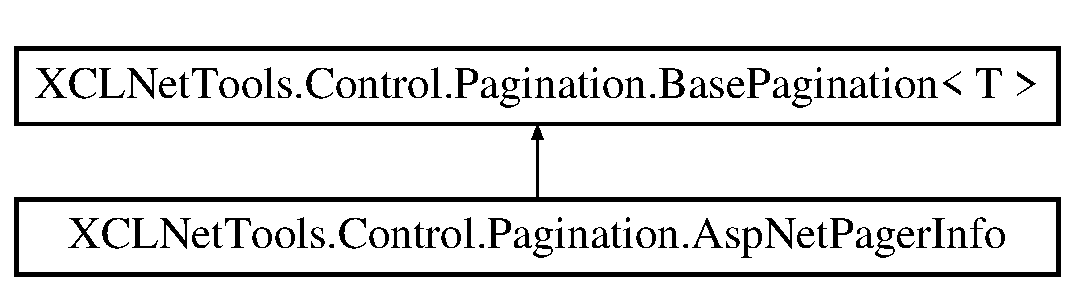
\includegraphics[height=2.000000cm]{class_x_c_l_net_tools_1_1_control_1_1_pagination_1_1_asp_net_pager_info}
\end{center}
\end{figure}
\subsection*{Public 成员函数}
\begin{DoxyCompactItemize}
\item 
\hyperlink{class_x_c_l_net_tools_1_1_control_1_1_pagination_1_1_asp_net_pager_info_aef75d024dd66cc9d75cd61d4dddcb27b}{Asp\-Net\-Pager\-Info} (Wuqi.\-Webdiyer.\-Asp\-Net\-Pager pager, int page\-Index, int page\-Size, int record\-Count)
\begin{DoxyCompactList}\small\item\em 构造函数 \end{DoxyCompactList}\item 
override void \hyperlink{class_x_c_l_net_tools_1_1_control_1_1_pagination_1_1_asp_net_pager_info_a46b208799b1d020c45571657c707ddf0}{Init\-Pager} ()
\begin{DoxyCompactList}\small\item\em 分页控件初始化 \end{DoxyCompactList}\end{DoxyCompactItemize}
\subsection*{额外继承的成员函数}


\subsection{详细描述}
Asp\-Net\-Pager分页 分页控件来源:http\-://www.webdiyer.\-com/aspnetpager/ 



在文件 Asp\-Net\-Pager\-Info.\-cs 第 7 行定义.



\subsection{构造及析构函数说明}
\hypertarget{class_x_c_l_net_tools_1_1_control_1_1_pagination_1_1_asp_net_pager_info_aef75d024dd66cc9d75cd61d4dddcb27b}{\index{X\-C\-L\-Net\-Tools\-::\-Control\-::\-Pagination\-::\-Asp\-Net\-Pager\-Info@{X\-C\-L\-Net\-Tools\-::\-Control\-::\-Pagination\-::\-Asp\-Net\-Pager\-Info}!Asp\-Net\-Pager\-Info@{Asp\-Net\-Pager\-Info}}
\index{Asp\-Net\-Pager\-Info@{Asp\-Net\-Pager\-Info}!XCLNetTools::Control::Pagination::AspNetPagerInfo@{X\-C\-L\-Net\-Tools\-::\-Control\-::\-Pagination\-::\-Asp\-Net\-Pager\-Info}}
\subsubsection[{Asp\-Net\-Pager\-Info}]{\setlength{\rightskip}{0pt plus 5cm}X\-C\-L\-Net\-Tools.\-Control.\-Pagination.\-Asp\-Net\-Pager\-Info.\-Asp\-Net\-Pager\-Info (
\begin{DoxyParamCaption}
\item[{Wuqi.\-Webdiyer.\-Asp\-Net\-Pager}]{pager, }
\item[{int}]{page\-Index, }
\item[{int}]{page\-Size, }
\item[{int}]{record\-Count}
\end{DoxyParamCaption}
)}}\label{class_x_c_l_net_tools_1_1_control_1_1_pagination_1_1_asp_net_pager_info_aef75d024dd66cc9d75cd61d4dddcb27b}


构造函数 


\begin{DoxyParams}{参数}
{\em pager} & 分页控件对象\\
\hline
{\em page\-Index} & 当前页码\\
\hline
{\em page\-Size} & 每页最多显示的记录数\\
\hline
{\em record\-Count} & 记录总数\\
\hline
\end{DoxyParams}


在文件 Asp\-Net\-Pager\-Info.\-cs 第 16 行定义.



\subsection{成员函数说明}
\hypertarget{class_x_c_l_net_tools_1_1_control_1_1_pagination_1_1_asp_net_pager_info_a46b208799b1d020c45571657c707ddf0}{\index{X\-C\-L\-Net\-Tools\-::\-Control\-::\-Pagination\-::\-Asp\-Net\-Pager\-Info@{X\-C\-L\-Net\-Tools\-::\-Control\-::\-Pagination\-::\-Asp\-Net\-Pager\-Info}!Init\-Pager@{Init\-Pager}}
\index{Init\-Pager@{Init\-Pager}!XCLNetTools::Control::Pagination::AspNetPagerInfo@{X\-C\-L\-Net\-Tools\-::\-Control\-::\-Pagination\-::\-Asp\-Net\-Pager\-Info}}
\subsubsection[{Init\-Pager}]{\setlength{\rightskip}{0pt plus 5cm}override void X\-C\-L\-Net\-Tools.\-Control.\-Pagination.\-Asp\-Net\-Pager\-Info.\-Init\-Pager (
\begin{DoxyParamCaption}
{}
\end{DoxyParamCaption}
)\hspace{0.3cm}{\ttfamily [virtual]}}}\label{class_x_c_l_net_tools_1_1_control_1_1_pagination_1_1_asp_net_pager_info_a46b208799b1d020c45571657c707ddf0}


分页控件初始化 



重载 \hyperlink{class_x_c_l_net_tools_1_1_control_1_1_pagination_1_1_base_pagination_3_01_t_01_4_ab3485196d5422f857f29f96bfbb2faa9}{X\-C\-L\-Net\-Tools.\-Control.\-Pagination.\-Base\-Pagination$<$ T $>$} .



在文件 Asp\-Net\-Pager\-Info.\-cs 第 24 行定义.



该类的文档由以下文件生成\-:\begin{DoxyCompactItemize}
\item 
Control/\-Pagination/\hyperlink{_asp_net_pager_info_8cs}{Asp\-Net\-Pager\-Info.\-cs}\end{DoxyCompactItemize}

\hypertarget{class_x_c_l_net_tools_1_1_encode_1_1_base64}{\section{X\-C\-L\-Net\-Tools.\-Encode.\-Base64类 参考}
\label{class_x_c_l_net_tools_1_1_encode_1_1_base64}\index{X\-C\-L\-Net\-Tools.\-Encode.\-Base64@{X\-C\-L\-Net\-Tools.\-Encode.\-Base64}}
}


base64相关  


\subsection*{静态 Public 成员函数}
\begin{DoxyCompactItemize}
\item 
static string \hyperlink{class_x_c_l_net_tools_1_1_encode_1_1_base64_a5a2afb86c63424b3aa879c8dafd82810}{Base64\-Code} (string Message)
\begin{DoxyCompactList}\small\item\em Base64加密 \end{DoxyCompactList}\item 
static string \hyperlink{class_x_c_l_net_tools_1_1_encode_1_1_base64_a0ba1e107c13f66936a16bb512b734d9f}{Base64\-Decode} (string Message)
\begin{DoxyCompactList}\small\item\em Base64解密 \end{DoxyCompactList}\end{DoxyCompactItemize}


\subsection{详细描述}
base64相关 



在文件 Base64.\-cs 第 30 行定义.



\subsection{成员函数说明}
\hypertarget{class_x_c_l_net_tools_1_1_encode_1_1_base64_a5a2afb86c63424b3aa879c8dafd82810}{\index{X\-C\-L\-Net\-Tools\-::\-Encode\-::\-Base64@{X\-C\-L\-Net\-Tools\-::\-Encode\-::\-Base64}!Base64\-Code@{Base64\-Code}}
\index{Base64\-Code@{Base64\-Code}!XCLNetTools::Encode::Base64@{X\-C\-L\-Net\-Tools\-::\-Encode\-::\-Base64}}
\subsubsection[{Base64\-Code}]{\setlength{\rightskip}{0pt plus 5cm}static string X\-C\-L\-Net\-Tools.\-Encode.\-Base64.\-Base64\-Code (
\begin{DoxyParamCaption}
\item[{string}]{Message}
\end{DoxyParamCaption}
)\hspace{0.3cm}{\ttfamily [static]}}}\label{class_x_c_l_net_tools_1_1_encode_1_1_base64_a5a2afb86c63424b3aa879c8dafd82810}


Base64加密 


\begin{DoxyParams}{参数}
{\em \hyperlink{namespace_x_c_l_net_tools_1_1_message}{Message}} & \\
\hline
\end{DoxyParams}
\begin{DoxyReturn}{返回}

\end{DoxyReturn}


在文件 Base64.\-cs 第 37 行定义.

\hypertarget{class_x_c_l_net_tools_1_1_encode_1_1_base64_a0ba1e107c13f66936a16bb512b734d9f}{\index{X\-C\-L\-Net\-Tools\-::\-Encode\-::\-Base64@{X\-C\-L\-Net\-Tools\-::\-Encode\-::\-Base64}!Base64\-Decode@{Base64\-Decode}}
\index{Base64\-Decode@{Base64\-Decode}!XCLNetTools::Encode::Base64@{X\-C\-L\-Net\-Tools\-::\-Encode\-::\-Base64}}
\subsubsection[{Base64\-Decode}]{\setlength{\rightskip}{0pt plus 5cm}static string X\-C\-L\-Net\-Tools.\-Encode.\-Base64.\-Base64\-Decode (
\begin{DoxyParamCaption}
\item[{string}]{Message}
\end{DoxyParamCaption}
)\hspace{0.3cm}{\ttfamily [static]}}}\label{class_x_c_l_net_tools_1_1_encode_1_1_base64_a0ba1e107c13f66936a16bb512b734d9f}


Base64解密 


\begin{DoxyParams}{参数}
{\em \hyperlink{namespace_x_c_l_net_tools_1_1_message}{Message}} & \\
\hline
\end{DoxyParams}
\begin{DoxyReturn}{返回}

\end{DoxyReturn}


在文件 Base64.\-cs 第 48 行定义.



该类的文档由以下文件生成\-:\begin{DoxyCompactItemize}
\item 
D\-:/\-My\-Data/\-My\-Git/\-Git\-Hub/\-X\-C\-L\-Net\-Tools/\-X\-C\-L\-Net\-Tools/\-Encode/\hyperlink{_base64_8cs}{Base64.\-cs}\end{DoxyCompactItemize}

\hypertarget{class_x_c_l_net_tools_1_1_control_1_1_pagination_1_1_base_pagination_3_01_t_01_4}{\section{X\-C\-L\-Net\-Tools.\-Control.\-Pagination.\-Base\-Pagination$<$ T $>$ 模板类 参考}
\label{class_x_c_l_net_tools_1_1_control_1_1_pagination_1_1_base_pagination_3_01_t_01_4}\index{X\-C\-L\-Net\-Tools.\-Control.\-Pagination.\-Base\-Pagination$<$ T $>$@{X\-C\-L\-Net\-Tools.\-Control.\-Pagination.\-Base\-Pagination$<$ T $>$}}
}


分页接口  


类 X\-C\-L\-Net\-Tools.\-Control.\-Pagination.\-Base\-Pagination$<$ T $>$ 继承关系图\-:\begin{figure}[H]
\begin{center}
\leavevmode
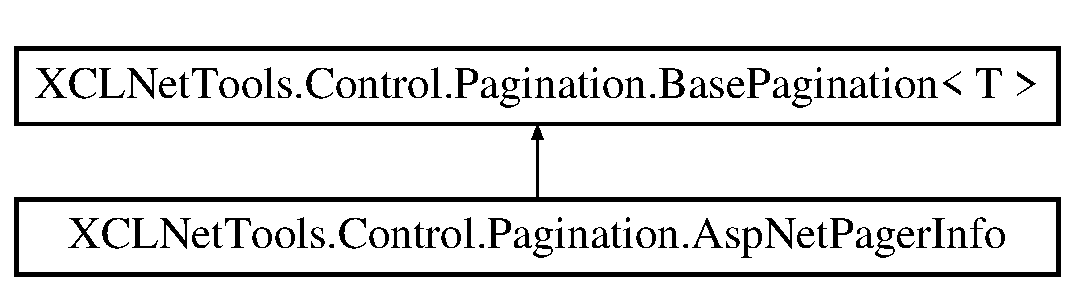
\includegraphics[height=2.000000cm]{class_x_c_l_net_tools_1_1_control_1_1_pagination_1_1_base_pagination_3_01_t_01_4}
\end{center}
\end{figure}
\subsection*{Public 成员函数}
\begin{DoxyCompactItemize}
\item 
\hyperlink{class_x_c_l_net_tools_1_1_control_1_1_pagination_1_1_base_pagination_3_01_t_01_4_ae9e336c1452804e7d4de12ea9fa3ddde}{Base\-Pagination} (T pager, int page\-Index, int page\-Size, int record\-Count)
\begin{DoxyCompactList}\small\item\em 构造函数 \end{DoxyCompactList}\item 
virtual void \hyperlink{class_x_c_l_net_tools_1_1_control_1_1_pagination_1_1_base_pagination_3_01_t_01_4_ab3485196d5422f857f29f96bfbb2faa9}{Init\-Pager} ()
\begin{DoxyCompactList}\small\item\em 分页初始化 \end{DoxyCompactList}\end{DoxyCompactItemize}
\subsection*{属性}
\begin{DoxyCompactItemize}
\item 
T \hyperlink{class_x_c_l_net_tools_1_1_control_1_1_pagination_1_1_base_pagination_3_01_t_01_4_ae0cfdba3ea23387da4b851c4d695d0a0}{Pager}\hspace{0.3cm}{\ttfamily  \mbox{[}get, set\mbox{]}}
\begin{DoxyCompactList}\small\item\em 当前分页控件 \end{DoxyCompactList}\item 
\hyperlink{class_x_c_l_net_tools_1_1_entity_1_1_pager_info}{X\-C\-L\-Net\-Tools.\-Entity.\-Pager\-Info} \hyperlink{class_x_c_l_net_tools_1_1_control_1_1_pagination_1_1_base_pagination_3_01_t_01_4_ae27d645cd692bb7471bc6236c59496a3}{Pager\-Info}\hspace{0.3cm}{\ttfamily  \mbox{[}get, set\mbox{]}}
\begin{DoxyCompactList}\small\item\em 分页信息 \end{DoxyCompactList}\end{DoxyCompactItemize}


\subsection{详细描述}
分页接口 



在文件 Base\-Pagination.\-cs 第 27 行定义.



\subsection{构造及析构函数说明}
\hypertarget{class_x_c_l_net_tools_1_1_control_1_1_pagination_1_1_base_pagination_3_01_t_01_4_ae9e336c1452804e7d4de12ea9fa3ddde}{\index{X\-C\-L\-Net\-Tools\-::\-Control\-::\-Pagination\-::\-Base\-Pagination$<$ T $>$@{X\-C\-L\-Net\-Tools\-::\-Control\-::\-Pagination\-::\-Base\-Pagination$<$ T $>$}!Base\-Pagination@{Base\-Pagination}}
\index{Base\-Pagination@{Base\-Pagination}!XCLNetTools::Control::Pagination::BasePagination< T >@{X\-C\-L\-Net\-Tools\-::\-Control\-::\-Pagination\-::\-Base\-Pagination$<$ T $>$}}
\subsubsection[{Base\-Pagination}]{\setlength{\rightskip}{0pt plus 5cm}X\-C\-L\-Net\-Tools.\-Control.\-Pagination.\-Base\-Pagination$<$ T $>$.Base\-Pagination (
\begin{DoxyParamCaption}
\item[{T}]{pager, }
\item[{int}]{page\-Index, }
\item[{int}]{page\-Size, }
\item[{int}]{record\-Count}
\end{DoxyParamCaption}
)}}\label{class_x_c_l_net_tools_1_1_control_1_1_pagination_1_1_base_pagination_3_01_t_01_4_ae9e336c1452804e7d4de12ea9fa3ddde}


构造函数 


\begin{DoxyParams}{参数}
{\em pager} & 分页控件对象\\
\hline
{\em page\-Index} & 当前页码\\
\hline
{\em page\-Size} & 每页最多显示的记录数\\
\hline
{\em record\-Count} & 记录总数\\
\hline
\end{DoxyParams}


在文件 Base\-Pagination.\-cs 第 40 行定义.



\subsection{成员函数说明}
\hypertarget{class_x_c_l_net_tools_1_1_control_1_1_pagination_1_1_base_pagination_3_01_t_01_4_ab3485196d5422f857f29f96bfbb2faa9}{\index{X\-C\-L\-Net\-Tools\-::\-Control\-::\-Pagination\-::\-Base\-Pagination$<$ T $>$@{X\-C\-L\-Net\-Tools\-::\-Control\-::\-Pagination\-::\-Base\-Pagination$<$ T $>$}!Init\-Pager@{Init\-Pager}}
\index{Init\-Pager@{Init\-Pager}!XCLNetTools::Control::Pagination::BasePagination< T >@{X\-C\-L\-Net\-Tools\-::\-Control\-::\-Pagination\-::\-Base\-Pagination$<$ T $>$}}
\subsubsection[{Init\-Pager}]{\setlength{\rightskip}{0pt plus 5cm}virtual void X\-C\-L\-Net\-Tools.\-Control.\-Pagination.\-Base\-Pagination$<$ T $>$.Init\-Pager (
\begin{DoxyParamCaption}
{}
\end{DoxyParamCaption}
)\hspace{0.3cm}{\ttfamily [virtual]}}}\label{class_x_c_l_net_tools_1_1_control_1_1_pagination_1_1_base_pagination_3_01_t_01_4_ab3485196d5422f857f29f96bfbb2faa9}


分页初始化 



被 \hyperlink{class_x_c_l_net_tools_1_1_control_1_1_pagination_1_1_asp_net_pager_info_a46b208799b1d020c45571657c707ddf0}{X\-C\-L\-Net\-Tools.\-Control.\-Pagination.\-Asp\-Net\-Pager\-Info} 重载.



在文件 Base\-Pagination.\-cs 第 60 行定义.



\subsection{属性说明}
\hypertarget{class_x_c_l_net_tools_1_1_control_1_1_pagination_1_1_base_pagination_3_01_t_01_4_ae0cfdba3ea23387da4b851c4d695d0a0}{\index{X\-C\-L\-Net\-Tools\-::\-Control\-::\-Pagination\-::\-Base\-Pagination$<$ T $>$@{X\-C\-L\-Net\-Tools\-::\-Control\-::\-Pagination\-::\-Base\-Pagination$<$ T $>$}!Pager@{Pager}}
\index{Pager@{Pager}!XCLNetTools::Control::Pagination::BasePagination< T >@{X\-C\-L\-Net\-Tools\-::\-Control\-::\-Pagination\-::\-Base\-Pagination$<$ T $>$}}
\subsubsection[{Pager}]{\setlength{\rightskip}{0pt plus 5cm}T X\-C\-L\-Net\-Tools.\-Control.\-Pagination.\-Base\-Pagination$<$ T $>$.Pager\hspace{0.3cm}{\ttfamily [get]}, {\ttfamily [set]}}}\label{class_x_c_l_net_tools_1_1_control_1_1_pagination_1_1_base_pagination_3_01_t_01_4_ae0cfdba3ea23387da4b851c4d695d0a0}


当前分页控件 



在文件 Base\-Pagination.\-cs 第 50 行定义.

\hypertarget{class_x_c_l_net_tools_1_1_control_1_1_pagination_1_1_base_pagination_3_01_t_01_4_ae27d645cd692bb7471bc6236c59496a3}{\index{X\-C\-L\-Net\-Tools\-::\-Control\-::\-Pagination\-::\-Base\-Pagination$<$ T $>$@{X\-C\-L\-Net\-Tools\-::\-Control\-::\-Pagination\-::\-Base\-Pagination$<$ T $>$}!Pager\-Info@{Pager\-Info}}
\index{Pager\-Info@{Pager\-Info}!XCLNetTools::Control::Pagination::BasePagination< T >@{X\-C\-L\-Net\-Tools\-::\-Control\-::\-Pagination\-::\-Base\-Pagination$<$ T $>$}}
\subsubsection[{Pager\-Info}]{\setlength{\rightskip}{0pt plus 5cm}{\bf X\-C\-L\-Net\-Tools.\-Entity.\-Pager\-Info} X\-C\-L\-Net\-Tools.\-Control.\-Pagination.\-Base\-Pagination$<$ T $>$.Pager\-Info\hspace{0.3cm}{\ttfamily [get]}, {\ttfamily [set]}}}\label{class_x_c_l_net_tools_1_1_control_1_1_pagination_1_1_base_pagination_3_01_t_01_4_ae27d645cd692bb7471bc6236c59496a3}


分页信息 



在文件 Base\-Pagination.\-cs 第 55 行定义.



该类的文档由以下文件生成\-:\begin{DoxyCompactItemize}
\item 
D\-:/\-My\-Data/\-My\-Git/\-Git\-Hub/\-X\-C\-L\-Net\-Tools/\-X\-C\-L\-Net\-Tools/\-Control/\-Pagination/\hyperlink{_base_pagination_8cs}{Base\-Pagination.\-cs}\end{DoxyCompactItemize}

\hypertarget{class_x_c_l_net_tools_1_1_file_handler_1_1_bookmark}{}\section{X\+C\+L\+Net\+Tools.\+File\+Handler.\+Bookmark类 参考}
\label{class_x_c_l_net_tools_1_1_file_handler_1_1_bookmark}\index{X\+C\+L\+Net\+Tools.\+File\+Handler.\+Bookmark@{X\+C\+L\+Net\+Tools.\+File\+Handler.\+Bookmark}}


浏览器书签文件操作类  


\subsection*{静态 Public 成员函数}
\begin{DoxyCompactItemize}
\item 
static List$<$ \hyperlink{class_x_c_l_net_tools_1_1_entity_1_1_bookmark_entity}{X\+C\+L\+Net\+Tools.\+Entity.\+Bookmark\+Entity} $>$ \hyperlink{class_x_c_l_net_tools_1_1_file_handler_1_1_bookmark_ab84885635ae274703936c5c10ae0f67c}{Get\+Bookmark} (string path)
\begin{DoxyCompactList}\small\item\em 根据浏览器书签文件地址,返回list \end{DoxyCompactList}\end{DoxyCompactItemize}


\subsection{详细描述}
浏览器书签文件操作类 



在文件 Bookmark.\+cs 第 18 行定义.



\subsection{成员函数说明}
\mbox{\Hypertarget{class_x_c_l_net_tools_1_1_file_handler_1_1_bookmark_ab84885635ae274703936c5c10ae0f67c}\label{class_x_c_l_net_tools_1_1_file_handler_1_1_bookmark_ab84885635ae274703936c5c10ae0f67c}} 
\index{X\+C\+L\+Net\+Tools\+::\+File\+Handler\+::\+Bookmark@{X\+C\+L\+Net\+Tools\+::\+File\+Handler\+::\+Bookmark}!Get\+Bookmark@{Get\+Bookmark}}
\index{Get\+Bookmark@{Get\+Bookmark}!X\+C\+L\+Net\+Tools\+::\+File\+Handler\+::\+Bookmark@{X\+C\+L\+Net\+Tools\+::\+File\+Handler\+::\+Bookmark}}
\subsubsection{\texorpdfstring{Get\+Bookmark()}{GetBookmark()}}
{\footnotesize\ttfamily static List$<$\hyperlink{class_x_c_l_net_tools_1_1_entity_1_1_bookmark_entity}{X\+C\+L\+Net\+Tools.\+Entity.\+Bookmark\+Entity}$>$ X\+C\+L\+Net\+Tools.\+File\+Handler.\+Bookmark.\+Get\+Bookmark (\begin{DoxyParamCaption}\item[{string}]{path }\end{DoxyParamCaption})\hspace{0.3cm}{\ttfamily [static]}}



根据浏览器书签文件地址,返回list 


\begin{DoxyParams}{参数}
{\em path} & 书签文件地址\\
\hline
\end{DoxyParams}
\begin{DoxyReturn}{返回}
书签list
\end{DoxyReturn}


在文件 Bookmark.\+cs 第 25 行定义.



该类的文档由以下文件生成\+:\begin{DoxyCompactItemize}
\item 
D\+:/\+My\+Data/\+Git\+Hub/\+X\+C\+L\+Net\+Tools/\+X\+C\+L\+Net\+Tools/\+File\+Handler/\hyperlink{_bookmark_8cs}{Bookmark.\+cs}\end{DoxyCompactItemize}

\hypertarget{class_x_c_l_net_tools_1_1_entity_1_1_bookmark_entity}{\section{X\-C\-L\-Net\-Tools.\-Entity.\-Bookmark\-Entity类 参考}
\label{class_x_c_l_net_tools_1_1_entity_1_1_bookmark_entity}\index{X\-C\-L\-Net\-Tools.\-Entity.\-Bookmark\-Entity@{X\-C\-L\-Net\-Tools.\-Entity.\-Bookmark\-Entity}}
}


浏览器书签实体  


\subsection*{属性}
\begin{DoxyCompactItemize}
\item 
int \hyperlink{class_x_c_l_net_tools_1_1_entity_1_1_bookmark_entity_a827314c81aad0801f464f7359509baec}{Id}\hspace{0.3cm}{\ttfamily  \mbox{[}get, set\mbox{]}}
\begin{DoxyCompactList}\small\item\em 编号 \end{DoxyCompactList}\item 
int \hyperlink{class_x_c_l_net_tools_1_1_entity_1_1_bookmark_entity_afd3c2002aa8d5edeac06f6ef32ba7454}{Parent\-Id}\hspace{0.3cm}{\ttfamily  \mbox{[}get, set\mbox{]}}
\begin{DoxyCompactList}\small\item\em 父id \end{DoxyCompactList}\item 
bool \hyperlink{class_x_c_l_net_tools_1_1_entity_1_1_bookmark_entity_a025f1606c5b38103058567b3e08afe03}{Is\-Folder}\hspace{0.3cm}{\ttfamily  \mbox{[}get, set\mbox{]}}
\begin{DoxyCompactList}\small\item\em 是否为文件夹 \end{DoxyCompactList}\item 
string \hyperlink{class_x_c_l_net_tools_1_1_entity_1_1_bookmark_entity_a89ccb517e285bfdd17981a72f590bc1c}{Name}\hspace{0.3cm}{\ttfamily  \mbox{[}get, set\mbox{]}}
\begin{DoxyCompactList}\small\item\em 书签名称 \end{DoxyCompactList}\item 
string \hyperlink{class_x_c_l_net_tools_1_1_entity_1_1_bookmark_entity_af370dbfd32e8cde501e305c6999c077b}{Ico\-U\-R\-L}\hspace{0.3cm}{\ttfamily  \mbox{[}get, set\mbox{]}}
\begin{DoxyCompactList}\small\item\em ico图标地址 \end{DoxyCompactList}\item 
string \hyperlink{class_x_c_l_net_tools_1_1_entity_1_1_bookmark_entity_a88ebfe2441fd5804a82f5eaee1ce3232}{Url}\hspace{0.3cm}{\ttfamily  \mbox{[}get, set\mbox{]}}
\begin{DoxyCompactList}\small\item\em 书签链接 \end{DoxyCompactList}\end{DoxyCompactItemize}


\subsection{详细描述}
浏览器书签实体 



在文件 Bookmark\-Entity.\-cs 第 17 行定义.



\subsection{属性说明}
\hypertarget{class_x_c_l_net_tools_1_1_entity_1_1_bookmark_entity_af370dbfd32e8cde501e305c6999c077b}{\index{X\-C\-L\-Net\-Tools\-::\-Entity\-::\-Bookmark\-Entity@{X\-C\-L\-Net\-Tools\-::\-Entity\-::\-Bookmark\-Entity}!Ico\-U\-R\-L@{Ico\-U\-R\-L}}
\index{Ico\-U\-R\-L@{Ico\-U\-R\-L}!XCLNetTools::Entity::BookmarkEntity@{X\-C\-L\-Net\-Tools\-::\-Entity\-::\-Bookmark\-Entity}}
\subsubsection[{Ico\-U\-R\-L}]{\setlength{\rightskip}{0pt plus 5cm}string X\-C\-L\-Net\-Tools.\-Entity.\-Bookmark\-Entity.\-Ico\-U\-R\-L\hspace{0.3cm}{\ttfamily [get]}, {\ttfamily [set]}}}\label{class_x_c_l_net_tools_1_1_entity_1_1_bookmark_entity_af370dbfd32e8cde501e305c6999c077b}


ico图标地址 



在文件 Bookmark\-Entity.\-cs 第 42 行定义.

\hypertarget{class_x_c_l_net_tools_1_1_entity_1_1_bookmark_entity_a827314c81aad0801f464f7359509baec}{\index{X\-C\-L\-Net\-Tools\-::\-Entity\-::\-Bookmark\-Entity@{X\-C\-L\-Net\-Tools\-::\-Entity\-::\-Bookmark\-Entity}!Id@{Id}}
\index{Id@{Id}!XCLNetTools::Entity::BookmarkEntity@{X\-C\-L\-Net\-Tools\-::\-Entity\-::\-Bookmark\-Entity}}
\subsubsection[{Id}]{\setlength{\rightskip}{0pt plus 5cm}int X\-C\-L\-Net\-Tools.\-Entity.\-Bookmark\-Entity.\-Id\hspace{0.3cm}{\ttfamily [get]}, {\ttfamily [set]}}}\label{class_x_c_l_net_tools_1_1_entity_1_1_bookmark_entity_a827314c81aad0801f464f7359509baec}


编号 



在文件 Bookmark\-Entity.\-cs 第 22 行定义.

\hypertarget{class_x_c_l_net_tools_1_1_entity_1_1_bookmark_entity_a025f1606c5b38103058567b3e08afe03}{\index{X\-C\-L\-Net\-Tools\-::\-Entity\-::\-Bookmark\-Entity@{X\-C\-L\-Net\-Tools\-::\-Entity\-::\-Bookmark\-Entity}!Is\-Folder@{Is\-Folder}}
\index{Is\-Folder@{Is\-Folder}!XCLNetTools::Entity::BookmarkEntity@{X\-C\-L\-Net\-Tools\-::\-Entity\-::\-Bookmark\-Entity}}
\subsubsection[{Is\-Folder}]{\setlength{\rightskip}{0pt plus 5cm}bool X\-C\-L\-Net\-Tools.\-Entity.\-Bookmark\-Entity.\-Is\-Folder\hspace{0.3cm}{\ttfamily [get]}, {\ttfamily [set]}}}\label{class_x_c_l_net_tools_1_1_entity_1_1_bookmark_entity_a025f1606c5b38103058567b3e08afe03}


是否为文件夹 



在文件 Bookmark\-Entity.\-cs 第 32 行定义.

\hypertarget{class_x_c_l_net_tools_1_1_entity_1_1_bookmark_entity_a89ccb517e285bfdd17981a72f590bc1c}{\index{X\-C\-L\-Net\-Tools\-::\-Entity\-::\-Bookmark\-Entity@{X\-C\-L\-Net\-Tools\-::\-Entity\-::\-Bookmark\-Entity}!Name@{Name}}
\index{Name@{Name}!XCLNetTools::Entity::BookmarkEntity@{X\-C\-L\-Net\-Tools\-::\-Entity\-::\-Bookmark\-Entity}}
\subsubsection[{Name}]{\setlength{\rightskip}{0pt plus 5cm}string X\-C\-L\-Net\-Tools.\-Entity.\-Bookmark\-Entity.\-Name\hspace{0.3cm}{\ttfamily [get]}, {\ttfamily [set]}}}\label{class_x_c_l_net_tools_1_1_entity_1_1_bookmark_entity_a89ccb517e285bfdd17981a72f590bc1c}


书签名称 



在文件 Bookmark\-Entity.\-cs 第 37 行定义.

\hypertarget{class_x_c_l_net_tools_1_1_entity_1_1_bookmark_entity_afd3c2002aa8d5edeac06f6ef32ba7454}{\index{X\-C\-L\-Net\-Tools\-::\-Entity\-::\-Bookmark\-Entity@{X\-C\-L\-Net\-Tools\-::\-Entity\-::\-Bookmark\-Entity}!Parent\-Id@{Parent\-Id}}
\index{Parent\-Id@{Parent\-Id}!XCLNetTools::Entity::BookmarkEntity@{X\-C\-L\-Net\-Tools\-::\-Entity\-::\-Bookmark\-Entity}}
\subsubsection[{Parent\-Id}]{\setlength{\rightskip}{0pt plus 5cm}int X\-C\-L\-Net\-Tools.\-Entity.\-Bookmark\-Entity.\-Parent\-Id\hspace{0.3cm}{\ttfamily [get]}, {\ttfamily [set]}}}\label{class_x_c_l_net_tools_1_1_entity_1_1_bookmark_entity_afd3c2002aa8d5edeac06f6ef32ba7454}


父id 



在文件 Bookmark\-Entity.\-cs 第 27 行定义.

\hypertarget{class_x_c_l_net_tools_1_1_entity_1_1_bookmark_entity_a88ebfe2441fd5804a82f5eaee1ce3232}{\index{X\-C\-L\-Net\-Tools\-::\-Entity\-::\-Bookmark\-Entity@{X\-C\-L\-Net\-Tools\-::\-Entity\-::\-Bookmark\-Entity}!Url@{Url}}
\index{Url@{Url}!XCLNetTools::Entity::BookmarkEntity@{X\-C\-L\-Net\-Tools\-::\-Entity\-::\-Bookmark\-Entity}}
\subsubsection[{Url}]{\setlength{\rightskip}{0pt plus 5cm}string X\-C\-L\-Net\-Tools.\-Entity.\-Bookmark\-Entity.\-Url\hspace{0.3cm}{\ttfamily [get]}, {\ttfamily [set]}}}\label{class_x_c_l_net_tools_1_1_entity_1_1_bookmark_entity_a88ebfe2441fd5804a82f5eaee1ce3232}


书签链接 



在文件 Bookmark\-Entity.\-cs 第 47 行定义.



该类的文档由以下文件生成\-:\begin{DoxyCompactItemize}
\item 
D\-:/\-My\-Data/\-My\-Git/\-Git\-Hub/\-X\-C\-L\-Net\-Tools/\-X\-C\-L\-Net\-Tools/\-Entity/\hyperlink{_bookmark_entity_8cs}{Bookmark\-Entity.\-cs}\end{DoxyCompactItemize}

\hypertarget{class_x_c_l_net_tools_1_1_cache_1_1_cache_class}{\section{X\-C\-L\-Net\-Tools.\-Cache.\-Cache\-Class类 参考}
\label{class_x_c_l_net_tools_1_1_cache_1_1_cache_class}\index{X\-C\-L\-Net\-Tools.\-Cache.\-Cache\-Class@{X\-C\-L\-Net\-Tools.\-Cache.\-Cache\-Class}}
}


缓存相关的操作类  


\subsection*{静态 Public 成员函数}
\begin{DoxyCompactItemize}
\item 
static object \hyperlink{class_x_c_l_net_tools_1_1_cache_1_1_cache_class_aa4eb429181d14c79040ea957bb4b8308}{Get\-Cache} (string Cache\-Key)
\begin{DoxyCompactList}\small\item\em 获取当前应用程序指定\-Cache\-Key的\-Cache值 \end{DoxyCompactList}\item 
static void \hyperlink{class_x_c_l_net_tools_1_1_cache_1_1_cache_class_a1f815a266c55067bab54e36c276ea82b}{Set\-Cache} (string Cache\-Key, object obj\-Object)
\begin{DoxyCompactList}\small\item\em 设置当前应用程序指定\-Cache\-Key的\-Cache值 \end{DoxyCompactList}\item 
static void \hyperlink{class_x_c_l_net_tools_1_1_cache_1_1_cache_class_a12454bcf0c4d79e76937bbd927df631e}{Set\-Cache} (string Cache\-Key, object obj\-Object, Date\-Time absolute\-Expiration, Time\-Span sliding\-Expiration)
\begin{DoxyCompactList}\small\item\em 设置当前应用程序指定\-Cache\-Key的\-Cache值 \end{DoxyCompactList}\item 
static void \hyperlink{class_x_c_l_net_tools_1_1_cache_1_1_cache_class_afeab3c01d1a7b41007235b97f3fbaa35}{Clear} (string key)
\begin{DoxyCompactList}\small\item\em 删除指定缓存 \end{DoxyCompactList}\item 
static bool \hyperlink{class_x_c_l_net_tools_1_1_cache_1_1_cache_class_aa7640102a9327d10ff130c69b724e27b}{Exists} (string key)
\begin{DoxyCompactList}\small\item\em 指定缓存是否存在 \end{DoxyCompactList}\item 
static void \hyperlink{class_x_c_l_net_tools_1_1_cache_1_1_cache_class_a36ade93bd935dbad5740285d48e2c5e6}{Remove\-All\-Cache} ()
\begin{DoxyCompactList}\small\item\em 移除全部缓存 \end{DoxyCompactList}\end{DoxyCompactItemize}


\subsection{详细描述}
缓存相关的操作类 



在文件 Cache\-Class.\-cs 第 31 行定义.



\subsection{成员函数说明}
\hypertarget{class_x_c_l_net_tools_1_1_cache_1_1_cache_class_afeab3c01d1a7b41007235b97f3fbaa35}{\index{X\-C\-L\-Net\-Tools\-::\-Cache\-::\-Cache\-Class@{X\-C\-L\-Net\-Tools\-::\-Cache\-::\-Cache\-Class}!Clear@{Clear}}
\index{Clear@{Clear}!XCLNetTools::Cache::CacheClass@{X\-C\-L\-Net\-Tools\-::\-Cache\-::\-Cache\-Class}}
\subsubsection[{Clear}]{\setlength{\rightskip}{0pt plus 5cm}static void X\-C\-L\-Net\-Tools.\-Cache.\-Cache\-Class.\-Clear (
\begin{DoxyParamCaption}
\item[{string}]{key}
\end{DoxyParamCaption}
)\hspace{0.3cm}{\ttfamily [static]}}}\label{class_x_c_l_net_tools_1_1_cache_1_1_cache_class_afeab3c01d1a7b41007235b97f3fbaa35}


删除指定缓存 


\begin{DoxyParams}{参数}
{\em key} & 缓存key名\\
\hline
\end{DoxyParams}


在文件 Cache\-Class.\-cs 第 72 行定义.

\hypertarget{class_x_c_l_net_tools_1_1_cache_1_1_cache_class_aa7640102a9327d10ff130c69b724e27b}{\index{X\-C\-L\-Net\-Tools\-::\-Cache\-::\-Cache\-Class@{X\-C\-L\-Net\-Tools\-::\-Cache\-::\-Cache\-Class}!Exists@{Exists}}
\index{Exists@{Exists}!XCLNetTools::Cache::CacheClass@{X\-C\-L\-Net\-Tools\-::\-Cache\-::\-Cache\-Class}}
\subsubsection[{Exists}]{\setlength{\rightskip}{0pt plus 5cm}static bool X\-C\-L\-Net\-Tools.\-Cache.\-Cache\-Class.\-Exists (
\begin{DoxyParamCaption}
\item[{string}]{key}
\end{DoxyParamCaption}
)\hspace{0.3cm}{\ttfamily [static]}}}\label{class_x_c_l_net_tools_1_1_cache_1_1_cache_class_aa7640102a9327d10ff130c69b724e27b}


指定缓存是否存在 


\begin{DoxyParams}{参数}
{\em key} & 缓存名\\
\hline
\end{DoxyParams}
\begin{DoxyReturn}{返回}
true\-:存在
\end{DoxyReturn}


在文件 Cache\-Class.\-cs 第 83 行定义.

\hypertarget{class_x_c_l_net_tools_1_1_cache_1_1_cache_class_aa4eb429181d14c79040ea957bb4b8308}{\index{X\-C\-L\-Net\-Tools\-::\-Cache\-::\-Cache\-Class@{X\-C\-L\-Net\-Tools\-::\-Cache\-::\-Cache\-Class}!Get\-Cache@{Get\-Cache}}
\index{Get\-Cache@{Get\-Cache}!XCLNetTools::Cache::CacheClass@{X\-C\-L\-Net\-Tools\-::\-Cache\-::\-Cache\-Class}}
\subsubsection[{Get\-Cache}]{\setlength{\rightskip}{0pt plus 5cm}static object X\-C\-L\-Net\-Tools.\-Cache.\-Cache\-Class.\-Get\-Cache (
\begin{DoxyParamCaption}
\item[{string}]{Cache\-Key}
\end{DoxyParamCaption}
)\hspace{0.3cm}{\ttfamily [static]}}}\label{class_x_c_l_net_tools_1_1_cache_1_1_cache_class_aa4eb429181d14c79040ea957bb4b8308}


获取当前应用程序指定\-Cache\-Key的\-Cache值 


\begin{DoxyParams}{参数}
{\em Cache\-Key} & 缓存key名\\
\hline
\end{DoxyParams}
\begin{DoxyReturn}{返回}
该缓存的值
\end{DoxyReturn}


在文件 Cache\-Class.\-cs 第 38 行定义.

\hypertarget{class_x_c_l_net_tools_1_1_cache_1_1_cache_class_a36ade93bd935dbad5740285d48e2c5e6}{\index{X\-C\-L\-Net\-Tools\-::\-Cache\-::\-Cache\-Class@{X\-C\-L\-Net\-Tools\-::\-Cache\-::\-Cache\-Class}!Remove\-All\-Cache@{Remove\-All\-Cache}}
\index{Remove\-All\-Cache@{Remove\-All\-Cache}!XCLNetTools::Cache::CacheClass@{X\-C\-L\-Net\-Tools\-::\-Cache\-::\-Cache\-Class}}
\subsubsection[{Remove\-All\-Cache}]{\setlength{\rightskip}{0pt plus 5cm}static void X\-C\-L\-Net\-Tools.\-Cache.\-Cache\-Class.\-Remove\-All\-Cache (
\begin{DoxyParamCaption}
{}
\end{DoxyParamCaption}
)\hspace{0.3cm}{\ttfamily [static]}}}\label{class_x_c_l_net_tools_1_1_cache_1_1_cache_class_a36ade93bd935dbad5740285d48e2c5e6}


移除全部缓存 



在文件 Cache\-Class.\-cs 第 92 行定义.

\hypertarget{class_x_c_l_net_tools_1_1_cache_1_1_cache_class_a1f815a266c55067bab54e36c276ea82b}{\index{X\-C\-L\-Net\-Tools\-::\-Cache\-::\-Cache\-Class@{X\-C\-L\-Net\-Tools\-::\-Cache\-::\-Cache\-Class}!Set\-Cache@{Set\-Cache}}
\index{Set\-Cache@{Set\-Cache}!XCLNetTools::Cache::CacheClass@{X\-C\-L\-Net\-Tools\-::\-Cache\-::\-Cache\-Class}}
\subsubsection[{Set\-Cache}]{\setlength{\rightskip}{0pt plus 5cm}static void X\-C\-L\-Net\-Tools.\-Cache.\-Cache\-Class.\-Set\-Cache (
\begin{DoxyParamCaption}
\item[{string}]{Cache\-Key, }
\item[{object}]{obj\-Object}
\end{DoxyParamCaption}
)\hspace{0.3cm}{\ttfamily [static]}}}\label{class_x_c_l_net_tools_1_1_cache_1_1_cache_class_a1f815a266c55067bab54e36c276ea82b}


设置当前应用程序指定\-Cache\-Key的\-Cache值 


\begin{DoxyParams}{参数}
{\em Cache\-Key} & 缓存key名\\
\hline
{\em obj\-Object} & 缓存key值\\
\hline
\end{DoxyParams}


在文件 Cache\-Class.\-cs 第 49 行定义.

\hypertarget{class_x_c_l_net_tools_1_1_cache_1_1_cache_class_a12454bcf0c4d79e76937bbd927df631e}{\index{X\-C\-L\-Net\-Tools\-::\-Cache\-::\-Cache\-Class@{X\-C\-L\-Net\-Tools\-::\-Cache\-::\-Cache\-Class}!Set\-Cache@{Set\-Cache}}
\index{Set\-Cache@{Set\-Cache}!XCLNetTools::Cache::CacheClass@{X\-C\-L\-Net\-Tools\-::\-Cache\-::\-Cache\-Class}}
\subsubsection[{Set\-Cache}]{\setlength{\rightskip}{0pt plus 5cm}static void X\-C\-L\-Net\-Tools.\-Cache.\-Cache\-Class.\-Set\-Cache (
\begin{DoxyParamCaption}
\item[{string}]{Cache\-Key, }
\item[{object}]{obj\-Object, }
\item[{Date\-Time}]{absolute\-Expiration, }
\item[{Time\-Span}]{sliding\-Expiration}
\end{DoxyParamCaption}
)\hspace{0.3cm}{\ttfamily [static]}}}\label{class_x_c_l_net_tools_1_1_cache_1_1_cache_class_a12454bcf0c4d79e76937bbd927df631e}


设置当前应用程序指定\-Cache\-Key的\-Cache值 


\begin{DoxyParams}{参数}
{\em Cache\-Key} & 缓存key名\\
\hline
{\em obj\-Object} & 缓存key值\\
\hline
{\em absolute\-Expiration} & 所插入对象将到期并被从缓存中移除的时间\\
\hline
{\em sliding\-Expiration} & 最后一次访问所插入对象时与该对象到期时之间的时间间隔\\
\hline
\end{DoxyParams}


在文件 Cache\-Class.\-cs 第 62 行定义.



该类的文档由以下文件生成\-:\begin{DoxyCompactItemize}
\item 
D\-:/\-My\-Data/\-My\-Git/\-Git\-Hub/\-X\-C\-L\-Net\-Tools/\-X\-C\-L\-Net\-Tools/\-Cache/\hyperlink{_cache_class_8cs}{Cache\-Class.\-cs}\end{DoxyCompactItemize}

\hypertarget{class_x_c_l_net_tools_1_1_language_1_1_c_n}{\section{X\-C\-L\-Net\-Tools.\-Language.\-C\-N类 参考}
\label{class_x_c_l_net_tools_1_1_language_1_1_c_n}\index{X\-C\-L\-Net\-Tools.\-Language.\-C\-N@{X\-C\-L\-Net\-Tools.\-Language.\-C\-N}}
}


中文处理  


\subsection*{静态 Public 成员函数}
\begin{DoxyCompactItemize}
\item 
static string \hyperlink{class_x_c_l_net_tools_1_1_language_1_1_c_n_a298b6a886b268ba4f667304e25cf5c93}{Convert\-To\-All\-Spell} (string str\-Chinese)
\begin{DoxyCompactList}\small\item\em 将汉字转化为全拼 \end{DoxyCompactList}\item 
static string \hyperlink{class_x_c_l_net_tools_1_1_language_1_1_c_n_adad5709d68f61a8cb7002ce6abf72c54}{Convert\-To\-First\-Spell} (string str\-Chinese)
\begin{DoxyCompactList}\small\item\em 将汉字转化为拼音首字母(大写) \end{DoxyCompactList}\item 
static string \hyperlink{class_x_c_l_net_tools_1_1_language_1_1_c_n_ae8a020bfe3d0b396edb88d8529decb29}{Get\-First\-Spell} (string char\-Chinese)
\begin{DoxyCompactList}\small\item\em 获取第一个汉字的首字母(大写); \end{DoxyCompactList}\item 
static string \hyperlink{class_x_c_l_net_tools_1_1_language_1_1_c_n_ac25cb893e8f56ae3ce28a04f4665c51d}{Convert\-First\-Spell} (string char\-Chinese)
\begin{DoxyCompactList}\small\item\em 获取第一个汉字的拼音 \end{DoxyCompactList}\end{DoxyCompactItemize}


\subsection{详细描述}
中文处理 



在文件 C\-N.\-cs 第 9 行定义.



\subsection{成员函数说明}
\hypertarget{class_x_c_l_net_tools_1_1_language_1_1_c_n_ac25cb893e8f56ae3ce28a04f4665c51d}{\index{X\-C\-L\-Net\-Tools\-::\-Language\-::\-C\-N@{X\-C\-L\-Net\-Tools\-::\-Language\-::\-C\-N}!Convert\-First\-Spell@{Convert\-First\-Spell}}
\index{Convert\-First\-Spell@{Convert\-First\-Spell}!XCLNetTools::Language::CN@{X\-C\-L\-Net\-Tools\-::\-Language\-::\-C\-N}}
\subsubsection[{Convert\-First\-Spell}]{\setlength{\rightskip}{0pt plus 5cm}static string X\-C\-L\-Net\-Tools.\-Language.\-C\-N.\-Convert\-First\-Spell (
\begin{DoxyParamCaption}
\item[{string}]{char\-Chinese}
\end{DoxyParamCaption}
)\hspace{0.3cm}{\ttfamily [static]}}}\label{class_x_c_l_net_tools_1_1_language_1_1_c_n_ac25cb893e8f56ae3ce28a04f4665c51d}


获取第一个汉字的拼音 



在文件 C\-N.\-cs 第 160 行定义.

\hypertarget{class_x_c_l_net_tools_1_1_language_1_1_c_n_a298b6a886b268ba4f667304e25cf5c93}{\index{X\-C\-L\-Net\-Tools\-::\-Language\-::\-C\-N@{X\-C\-L\-Net\-Tools\-::\-Language\-::\-C\-N}!Convert\-To\-All\-Spell@{Convert\-To\-All\-Spell}}
\index{Convert\-To\-All\-Spell@{Convert\-To\-All\-Spell}!XCLNetTools::Language::CN@{X\-C\-L\-Net\-Tools\-::\-Language\-::\-C\-N}}
\subsubsection[{Convert\-To\-All\-Spell}]{\setlength{\rightskip}{0pt plus 5cm}static string X\-C\-L\-Net\-Tools.\-Language.\-C\-N.\-Convert\-To\-All\-Spell (
\begin{DoxyParamCaption}
\item[{string}]{str\-Chinese}
\end{DoxyParamCaption}
)\hspace{0.3cm}{\ttfamily [static]}}}\label{class_x_c_l_net_tools_1_1_language_1_1_c_n_a298b6a886b268ba4f667304e25cf5c93}


将汉字转化为全拼 



在文件 C\-N.\-cs 第 75 行定义.

\hypertarget{class_x_c_l_net_tools_1_1_language_1_1_c_n_adad5709d68f61a8cb7002ce6abf72c54}{\index{X\-C\-L\-Net\-Tools\-::\-Language\-::\-C\-N@{X\-C\-L\-Net\-Tools\-::\-Language\-::\-C\-N}!Convert\-To\-First\-Spell@{Convert\-To\-First\-Spell}}
\index{Convert\-To\-First\-Spell@{Convert\-To\-First\-Spell}!XCLNetTools::Language::CN@{X\-C\-L\-Net\-Tools\-::\-Language\-::\-C\-N}}
\subsubsection[{Convert\-To\-First\-Spell}]{\setlength{\rightskip}{0pt plus 5cm}static string X\-C\-L\-Net\-Tools.\-Language.\-C\-N.\-Convert\-To\-First\-Spell (
\begin{DoxyParamCaption}
\item[{string}]{str\-Chinese}
\end{DoxyParamCaption}
)\hspace{0.3cm}{\ttfamily [static]}}}\label{class_x_c_l_net_tools_1_1_language_1_1_c_n_adad5709d68f61a8cb7002ce6abf72c54}


将汉字转化为拼音首字母(大写) 



在文件 C\-N.\-cs 第 119 行定义.

\hypertarget{class_x_c_l_net_tools_1_1_language_1_1_c_n_ae8a020bfe3d0b396edb88d8529decb29}{\index{X\-C\-L\-Net\-Tools\-::\-Language\-::\-C\-N@{X\-C\-L\-Net\-Tools\-::\-Language\-::\-C\-N}!Get\-First\-Spell@{Get\-First\-Spell}}
\index{Get\-First\-Spell@{Get\-First\-Spell}!XCLNetTools::Language::CN@{X\-C\-L\-Net\-Tools\-::\-Language\-::\-C\-N}}
\subsubsection[{Get\-First\-Spell}]{\setlength{\rightskip}{0pt plus 5cm}static string X\-C\-L\-Net\-Tools.\-Language.\-C\-N.\-Get\-First\-Spell (
\begin{DoxyParamCaption}
\item[{string}]{char\-Chinese}
\end{DoxyParamCaption}
)\hspace{0.3cm}{\ttfamily [static]}}}\label{class_x_c_l_net_tools_1_1_language_1_1_c_n_ae8a020bfe3d0b396edb88d8529decb29}


获取第一个汉字的首字母(大写); 



在文件 C\-N.\-cs 第 133 行定义.



该类的文档由以下文件生成\-:\begin{DoxyCompactItemize}
\item 
Language/\hyperlink{_c_n_8cs}{C\-N.\-cs}\end{DoxyCompactItemize}

\hypertarget{class_x_c_l_net_tools_1_1_file_handler_1_1_com_file}{\section{X\-C\-L\-Net\-Tools.\-File\-Handler.\-Com\-File类 参考}
\label{class_x_c_l_net_tools_1_1_file_handler_1_1_com_file}\index{X\-C\-L\-Net\-Tools.\-File\-Handler.\-Com\-File@{X\-C\-L\-Net\-Tools.\-File\-Handler.\-Com\-File}}
}


文件操作公共类  


\subsection*{静态 Public 成员函数}
\begin{DoxyCompactItemize}
\item 
static bool \hyperlink{class_x_c_l_net_tools_1_1_file_handler_1_1_com_file_a7cc80f663aa1e69cf43af4a902243cc3}{Delete\-File} (string file\-Path)
\begin{DoxyCompactList}\small\item\em 删除文件 \end{DoxyCompactList}\item 
static bool \hyperlink{class_x_c_l_net_tools_1_1_file_handler_1_1_com_file_ae8479a1330655aa229ed6222410b7823}{Copy\-File} (string src\-Path, string dst\-Path)
\begin{DoxyCompactList}\small\item\em 复制文件(若已存在目标文件则覆盖),若目标目录不存在,则自动创建 \end{DoxyCompactList}\item 
static bool \hyperlink{class_x_c_l_net_tools_1_1_file_handler_1_1_com_file_a1e917318b8b594c94d0fb50223f34648}{Copy\-File} (string src\-Path, string dst\-Path, bool overwrite)
\begin{DoxyCompactList}\small\item\em 复制文件,若目标目录不存在,则自动创建 \end{DoxyCompactList}\item 
static string\mbox{[}$\,$\mbox{]} \hyperlink{class_x_c_l_net_tools_1_1_file_handler_1_1_com_file_ae82ff285ff8d522f3d6096c26e70ce40}{Get\-Folder\-Files} (string path)
\begin{DoxyCompactList}\small\item\em 取得文件夹中的文件列表 \end{DoxyCompactList}\item 
static string\mbox{[}$\,$\mbox{]} \hyperlink{class_x_c_l_net_tools_1_1_file_handler_1_1_com_file_a674fdbb6dfba9453918df90642428caf}{Get\-Folder\-Files\-By\-Recursion} (string root\-Path)
\begin{DoxyCompactList}\small\item\em 递归获取指定文件夹下的所有文件路径 \end{DoxyCompactList}\item 
static void \hyperlink{class_x_c_l_net_tools_1_1_file_handler_1_1_com_file_a88a411e0efbbb5117f62ae15734b5a4b}{Down\-Load\-File} (string path, string real\-Name)
\begin{DoxyCompactList}\small\item\em 文件下载 \end{DoxyCompactList}\item 
static string \hyperlink{class_x_c_l_net_tools_1_1_file_handler_1_1_com_file_a7fd47f5dd58f607c4fad3bb596f2d7b6}{Get\-Save\-Directory} (string directory\-Path)
\begin{DoxyCompactList}\small\item\em 返回目录路径,若该目录不存在,则创建该目录 \end{DoxyCompactList}\item 
static string \hyperlink{class_x_c_l_net_tools_1_1_file_handler_1_1_com_file_a54bcd222d9060ea6ee9d64264caf9939}{Get\-File\-Folder\-Path} (string file\-Path)
\begin{DoxyCompactList}\small\item\em 获取文件所在的文件夹【不带'\textbackslash{}'】 \end{DoxyCompactList}\item 
static long \hyperlink{class_x_c_l_net_tools_1_1_file_handler_1_1_com_file_a14816af3acf91a20ded5325a889f8341}{Get\-File\-Size} (string file\-Path)
\begin{DoxyCompactList}\small\item\em 返回文件大小(字节) \end{DoxyCompactList}\item 
static bool \hyperlink{class_x_c_l_net_tools_1_1_file_handler_1_1_com_file_a9e413978309f59720a38228ad9c1aaa2}{Is\-Binary\-File} (string file\-Path)
\begin{DoxyCompactList}\small\item\em 判断文件是否是二进制文件 \end{DoxyCompactList}\item 
static bool \hyperlink{class_x_c_l_net_tools_1_1_file_handler_1_1_com_file_afddfff3c4a196399bc033df2b017b16c}{Is\-Text\-File} (string file\-Path)
\begin{DoxyCompactList}\small\item\em 判断文件是否是文本文件 \end{DoxyCompactList}\item 
static string \hyperlink{class_x_c_l_net_tools_1_1_file_handler_1_1_com_file_a98d090828121f63039a22838b065dfaa}{Map\-Path} (string path)
\begin{DoxyCompactList}\small\item\em 取得文件物理路径 \end{DoxyCompactList}\item 
static string \hyperlink{class_x_c_l_net_tools_1_1_file_handler_1_1_com_file_a87d1f27fa942e4682abc91f13ca79672}{Get\-Url\-Relative\-Path} (string root\-Path, string path)
\begin{DoxyCompactList}\small\item\em 根据指定文件的物理路径\-Path,将它转换为相对于\-Root\-Path的\-Url相对路径 例如: Get\-Url\-Relative\-Path(\char`\"{}\-C\-:\textbackslash{}\-Program Files\textbackslash{}\-Information\textbackslash{}\char`\"{},\char`\"{}\-C\-:\textbackslash{}\-Program Files\textbackslash{}\-Information\textbackslash{}\-A\textbackslash{}\-B\textbackslash{}\-C.\-txt\char`\"{})=$>$\char`\"{}\-A/\-B/\-C.\-txt\char`\"{} Get\-Url\-Relative\-Path(\char`\"{}\-C\-:\textbackslash{}\-Program Files\textbackslash{}\-Information\textbackslash{}\char`\"{},\char`\"{}\-C\-:\textbackslash{}\-A\textbackslash{}\-B\textbackslash{}\-C.\-txt\char`\"{})=$>$\char`\"{}../../\-A/\-B/\-C.\-txt\char`\"{} \end{DoxyCompactList}\item 
static string \hyperlink{class_x_c_l_net_tools_1_1_file_handler_1_1_com_file_ad13584770f8b195682bbaccf49d9f10d}{Get\-File\-Name} (string file\-Name, bool is\-With\-Ext=true)
\begin{DoxyCompactList}\small\item\em 获取文件名 \end{DoxyCompactList}\item 
static string \hyperlink{class_x_c_l_net_tools_1_1_file_handler_1_1_com_file_acc1c32c42fbd8c6e76f3a609af5e407f}{Get\-Random\-File\-Name} (string filename)
\begin{DoxyCompactList}\small\item\em \begin{DoxyVerb}<summary>
\end{DoxyVerb}
 给上传的文件随机命名 \end{DoxyCompactList}\item 
static string \hyperlink{class_x_c_l_net_tools_1_1_file_handler_1_1_com_file_ab93269a3eef81ae3afe9e502e202f209}{Get\-Ext\-Name} (string file\-Name)
\begin{DoxyCompactList}\small\item\em 取得文件扩展名(不包含小圆点)【小写】 \end{DoxyCompactList}\end{DoxyCompactItemize}


\subsection{详细描述}
文件操作公共类 



在文件 Com\-File.\-cs 第 35 行定义.



\subsection{成员函数说明}
\hypertarget{class_x_c_l_net_tools_1_1_file_handler_1_1_com_file_ae8479a1330655aa229ed6222410b7823}{\index{X\-C\-L\-Net\-Tools\-::\-File\-Handler\-::\-Com\-File@{X\-C\-L\-Net\-Tools\-::\-File\-Handler\-::\-Com\-File}!Copy\-File@{Copy\-File}}
\index{Copy\-File@{Copy\-File}!XCLNetTools::FileHandler::ComFile@{X\-C\-L\-Net\-Tools\-::\-File\-Handler\-::\-Com\-File}}
\subsubsection[{Copy\-File}]{\setlength{\rightskip}{0pt plus 5cm}static bool X\-C\-L\-Net\-Tools.\-File\-Handler.\-Com\-File.\-Copy\-File (
\begin{DoxyParamCaption}
\item[{string}]{src\-Path, }
\item[{string}]{dst\-Path}
\end{DoxyParamCaption}
)\hspace{0.3cm}{\ttfamily [static]}}}\label{class_x_c_l_net_tools_1_1_file_handler_1_1_com_file_ae8479a1330655aa229ed6222410b7823}


复制文件(若已存在目标文件则覆盖),若目标目录不存在,则自动创建 


\begin{DoxyParams}{参数}
{\em src\-Path} & 源文件\\
\hline
{\em dst\-Path} & 目标文件\\
\hline
\end{DoxyParams}
\begin{DoxyReturn}{返回}
复制成功返回\-T\-R\-U\-E,复制失败返回\-F\-A\-L\-S\-E.
\end{DoxyReturn}


在文件 Com\-File.\-cs 第 76 行定义.

\hypertarget{class_x_c_l_net_tools_1_1_file_handler_1_1_com_file_a1e917318b8b594c94d0fb50223f34648}{\index{X\-C\-L\-Net\-Tools\-::\-File\-Handler\-::\-Com\-File@{X\-C\-L\-Net\-Tools\-::\-File\-Handler\-::\-Com\-File}!Copy\-File@{Copy\-File}}
\index{Copy\-File@{Copy\-File}!XCLNetTools::FileHandler::ComFile@{X\-C\-L\-Net\-Tools\-::\-File\-Handler\-::\-Com\-File}}
\subsubsection[{Copy\-File}]{\setlength{\rightskip}{0pt plus 5cm}static bool X\-C\-L\-Net\-Tools.\-File\-Handler.\-Com\-File.\-Copy\-File (
\begin{DoxyParamCaption}
\item[{string}]{src\-Path, }
\item[{string}]{dst\-Path, }
\item[{bool}]{overwrite}
\end{DoxyParamCaption}
)\hspace{0.3cm}{\ttfamily [static]}}}\label{class_x_c_l_net_tools_1_1_file_handler_1_1_com_file_a1e917318b8b594c94d0fb50223f34648}


复制文件,若目标目录不存在,则自动创建 


\begin{DoxyParams}{参数}
{\em src\-Path} & 源文件\\
\hline
{\em dst\-Path} & 目标文件\\
\hline
{\em overwrite} & 是否覆盖目标文件\\
\hline
\end{DoxyParams}
\begin{DoxyReturn}{返回}
复制成功返回\-T\-R\-U\-E,复制失败返回\-F\-A\-L\-S\-E
\end{DoxyReturn}


在文件 Com\-File.\-cs 第 89 行定义.

\hypertarget{class_x_c_l_net_tools_1_1_file_handler_1_1_com_file_a7cc80f663aa1e69cf43af4a902243cc3}{\index{X\-C\-L\-Net\-Tools\-::\-File\-Handler\-::\-Com\-File@{X\-C\-L\-Net\-Tools\-::\-File\-Handler\-::\-Com\-File}!Delete\-File@{Delete\-File}}
\index{Delete\-File@{Delete\-File}!XCLNetTools::FileHandler::ComFile@{X\-C\-L\-Net\-Tools\-::\-File\-Handler\-::\-Com\-File}}
\subsubsection[{Delete\-File}]{\setlength{\rightskip}{0pt plus 5cm}static bool X\-C\-L\-Net\-Tools.\-File\-Handler.\-Com\-File.\-Delete\-File (
\begin{DoxyParamCaption}
\item[{string}]{file\-Path}
\end{DoxyParamCaption}
)\hspace{0.3cm}{\ttfamily [static]}}}\label{class_x_c_l_net_tools_1_1_file_handler_1_1_com_file_a7cc80f663aa1e69cf43af4a902243cc3}


删除文件 


\begin{DoxyParams}{参数}
{\em file\-Path} & 文件路径\\
\hline
\end{DoxyParams}
\begin{DoxyReturn}{返回}
若为true,则删除成功
\end{DoxyReturn}


在文件 Com\-File.\-cs 第 44 行定义.

\hypertarget{class_x_c_l_net_tools_1_1_file_handler_1_1_com_file_a88a411e0efbbb5117f62ae15734b5a4b}{\index{X\-C\-L\-Net\-Tools\-::\-File\-Handler\-::\-Com\-File@{X\-C\-L\-Net\-Tools\-::\-File\-Handler\-::\-Com\-File}!Down\-Load\-File@{Down\-Load\-File}}
\index{Down\-Load\-File@{Down\-Load\-File}!XCLNetTools::FileHandler::ComFile@{X\-C\-L\-Net\-Tools\-::\-File\-Handler\-::\-Com\-File}}
\subsubsection[{Down\-Load\-File}]{\setlength{\rightskip}{0pt plus 5cm}static void X\-C\-L\-Net\-Tools.\-File\-Handler.\-Com\-File.\-Down\-Load\-File (
\begin{DoxyParamCaption}
\item[{string}]{path, }
\item[{string}]{real\-Name}
\end{DoxyParamCaption}
)\hspace{0.3cm}{\ttfamily [static]}}}\label{class_x_c_l_net_tools_1_1_file_handler_1_1_com_file_a88a411e0efbbb5117f62ae15734b5a4b}


文件下载 


\begin{DoxyParams}{参数}
{\em path} & 文件链接(物理路径)\\
\hline
{\em real\-Name} & 要显示下载时的文件名\\
\hline
\end{DoxyParams}


在文件 Com\-File.\-cs 第 150 行定义.

\hypertarget{class_x_c_l_net_tools_1_1_file_handler_1_1_com_file_ab93269a3eef81ae3afe9e502e202f209}{\index{X\-C\-L\-Net\-Tools\-::\-File\-Handler\-::\-Com\-File@{X\-C\-L\-Net\-Tools\-::\-File\-Handler\-::\-Com\-File}!Get\-Ext\-Name@{Get\-Ext\-Name}}
\index{Get\-Ext\-Name@{Get\-Ext\-Name}!XCLNetTools::FileHandler::ComFile@{X\-C\-L\-Net\-Tools\-::\-File\-Handler\-::\-Com\-File}}
\subsubsection[{Get\-Ext\-Name}]{\setlength{\rightskip}{0pt plus 5cm}static string X\-C\-L\-Net\-Tools.\-File\-Handler.\-Com\-File.\-Get\-Ext\-Name (
\begin{DoxyParamCaption}
\item[{string}]{file\-Name}
\end{DoxyParamCaption}
)\hspace{0.3cm}{\ttfamily [static]}}}\label{class_x_c_l_net_tools_1_1_file_handler_1_1_com_file_ab93269a3eef81ae3afe9e502e202f209}


取得文件扩展名(不包含小圆点)【小写】 


\begin{DoxyParams}{参数}
{\em file\-Name} & 文件完整路径或文件名\\
\hline
\end{DoxyParams}
\begin{DoxyReturn}{返回}
文件扩展名(不包含小圆点)
\end{DoxyReturn}


在文件 Com\-File.\-cs 第 368 行定义.

\hypertarget{class_x_c_l_net_tools_1_1_file_handler_1_1_com_file_a54bcd222d9060ea6ee9d64264caf9939}{\index{X\-C\-L\-Net\-Tools\-::\-File\-Handler\-::\-Com\-File@{X\-C\-L\-Net\-Tools\-::\-File\-Handler\-::\-Com\-File}!Get\-File\-Folder\-Path@{Get\-File\-Folder\-Path}}
\index{Get\-File\-Folder\-Path@{Get\-File\-Folder\-Path}!XCLNetTools::FileHandler::ComFile@{X\-C\-L\-Net\-Tools\-::\-File\-Handler\-::\-Com\-File}}
\subsubsection[{Get\-File\-Folder\-Path}]{\setlength{\rightskip}{0pt plus 5cm}static string X\-C\-L\-Net\-Tools.\-File\-Handler.\-Com\-File.\-Get\-File\-Folder\-Path (
\begin{DoxyParamCaption}
\item[{string}]{file\-Path}
\end{DoxyParamCaption}
)\hspace{0.3cm}{\ttfamily [static]}}}\label{class_x_c_l_net_tools_1_1_file_handler_1_1_com_file_a54bcd222d9060ea6ee9d64264caf9939}


获取文件所在的文件夹【不带'\textbackslash{}'】 



在文件 Com\-File.\-cs 第 195 行定义.

\hypertarget{class_x_c_l_net_tools_1_1_file_handler_1_1_com_file_ad13584770f8b195682bbaccf49d9f10d}{\index{X\-C\-L\-Net\-Tools\-::\-File\-Handler\-::\-Com\-File@{X\-C\-L\-Net\-Tools\-::\-File\-Handler\-::\-Com\-File}!Get\-File\-Name@{Get\-File\-Name}}
\index{Get\-File\-Name@{Get\-File\-Name}!XCLNetTools::FileHandler::ComFile@{X\-C\-L\-Net\-Tools\-::\-File\-Handler\-::\-Com\-File}}
\subsubsection[{Get\-File\-Name}]{\setlength{\rightskip}{0pt plus 5cm}static string X\-C\-L\-Net\-Tools.\-File\-Handler.\-Com\-File.\-Get\-File\-Name (
\begin{DoxyParamCaption}
\item[{string}]{file\-Name, }
\item[{bool}]{is\-With\-Ext = {\ttfamily true}}
\end{DoxyParamCaption}
)\hspace{0.3cm}{\ttfamily [static]}}}\label{class_x_c_l_net_tools_1_1_file_handler_1_1_com_file_ad13584770f8b195682bbaccf49d9f10d}


获取文件名 


\begin{DoxyParams}{参数}
{\em file\-Name} & 路径(相对或绝对均可)\\
\hline
{\em is\-With\-Ext} & 是否包含扩展名\\
\hline
\end{DoxyParams}
\begin{DoxyReturn}{返回}
文件名
\end{DoxyReturn}


在文件 Com\-File.\-cs 第 328 行定义.

\hypertarget{class_x_c_l_net_tools_1_1_file_handler_1_1_com_file_a14816af3acf91a20ded5325a889f8341}{\index{X\-C\-L\-Net\-Tools\-::\-File\-Handler\-::\-Com\-File@{X\-C\-L\-Net\-Tools\-::\-File\-Handler\-::\-Com\-File}!Get\-File\-Size@{Get\-File\-Size}}
\index{Get\-File\-Size@{Get\-File\-Size}!XCLNetTools::FileHandler::ComFile@{X\-C\-L\-Net\-Tools\-::\-File\-Handler\-::\-Com\-File}}
\subsubsection[{Get\-File\-Size}]{\setlength{\rightskip}{0pt plus 5cm}static long X\-C\-L\-Net\-Tools.\-File\-Handler.\-Com\-File.\-Get\-File\-Size (
\begin{DoxyParamCaption}
\item[{string}]{file\-Path}
\end{DoxyParamCaption}
)\hspace{0.3cm}{\ttfamily [static]}}}\label{class_x_c_l_net_tools_1_1_file_handler_1_1_com_file_a14816af3acf91a20ded5325a889f8341}


返回文件大小(字节) 

\begin{DoxyReturn}{返回}
文件大小 byte
\end{DoxyReturn}


在文件 Com\-File.\-cs 第 208 行定义.

\hypertarget{class_x_c_l_net_tools_1_1_file_handler_1_1_com_file_ae82ff285ff8d522f3d6096c26e70ce40}{\index{X\-C\-L\-Net\-Tools\-::\-File\-Handler\-::\-Com\-File@{X\-C\-L\-Net\-Tools\-::\-File\-Handler\-::\-Com\-File}!Get\-Folder\-Files@{Get\-Folder\-Files}}
\index{Get\-Folder\-Files@{Get\-Folder\-Files}!XCLNetTools::FileHandler::ComFile@{X\-C\-L\-Net\-Tools\-::\-File\-Handler\-::\-Com\-File}}
\subsubsection[{Get\-Folder\-Files}]{\setlength{\rightskip}{0pt plus 5cm}static string \mbox{[}$\,$\mbox{]} X\-C\-L\-Net\-Tools.\-File\-Handler.\-Com\-File.\-Get\-Folder\-Files (
\begin{DoxyParamCaption}
\item[{string}]{path}
\end{DoxyParamCaption}
)\hspace{0.3cm}{\ttfamily [static]}}}\label{class_x_c_l_net_tools_1_1_file_handler_1_1_com_file_ae82ff285ff8d522f3d6096c26e70ce40}


取得文件夹中的文件列表 


\begin{DoxyParams}{参数}
{\em path} & 文件夹路径\\
\hline
\end{DoxyParams}
\begin{DoxyReturn}{返回}
字符串数组(存储了一个或多个文件名)
\end{DoxyReturn}


在文件 Com\-File.\-cs 第 105 行定义.

\hypertarget{class_x_c_l_net_tools_1_1_file_handler_1_1_com_file_a674fdbb6dfba9453918df90642428caf}{\index{X\-C\-L\-Net\-Tools\-::\-File\-Handler\-::\-Com\-File@{X\-C\-L\-Net\-Tools\-::\-File\-Handler\-::\-Com\-File}!Get\-Folder\-Files\-By\-Recursion@{Get\-Folder\-Files\-By\-Recursion}}
\index{Get\-Folder\-Files\-By\-Recursion@{Get\-Folder\-Files\-By\-Recursion}!XCLNetTools::FileHandler::ComFile@{X\-C\-L\-Net\-Tools\-::\-File\-Handler\-::\-Com\-File}}
\subsubsection[{Get\-Folder\-Files\-By\-Recursion}]{\setlength{\rightskip}{0pt plus 5cm}static string \mbox{[}$\,$\mbox{]} X\-C\-L\-Net\-Tools.\-File\-Handler.\-Com\-File.\-Get\-Folder\-Files\-By\-Recursion (
\begin{DoxyParamCaption}
\item[{string}]{root\-Path}
\end{DoxyParamCaption}
)\hspace{0.3cm}{\ttfamily [static]}}}\label{class_x_c_l_net_tools_1_1_file_handler_1_1_com_file_a674fdbb6dfba9453918df90642428caf}


递归获取指定文件夹下的所有文件路径 


\begin{DoxyParams}{参数}
{\em root\-Path} & 起始文件夹路径\\
\hline
\end{DoxyParams}
\begin{DoxyReturn}{返回}
文件路径数组
\end{DoxyReturn}


在文件 Com\-File.\-cs 第 115 行定义.

\hypertarget{class_x_c_l_net_tools_1_1_file_handler_1_1_com_file_acc1c32c42fbd8c6e76f3a609af5e407f}{\index{X\-C\-L\-Net\-Tools\-::\-File\-Handler\-::\-Com\-File@{X\-C\-L\-Net\-Tools\-::\-File\-Handler\-::\-Com\-File}!Get\-Random\-File\-Name@{Get\-Random\-File\-Name}}
\index{Get\-Random\-File\-Name@{Get\-Random\-File\-Name}!XCLNetTools::FileHandler::ComFile@{X\-C\-L\-Net\-Tools\-::\-File\-Handler\-::\-Com\-File}}
\subsubsection[{Get\-Random\-File\-Name}]{\setlength{\rightskip}{0pt plus 5cm}static string X\-C\-L\-Net\-Tools.\-File\-Handler.\-Com\-File.\-Get\-Random\-File\-Name (
\begin{DoxyParamCaption}
\item[{string}]{filename}
\end{DoxyParamCaption}
)\hspace{0.3cm}{\ttfamily [static]}}}\label{class_x_c_l_net_tools_1_1_file_handler_1_1_com_file_acc1c32c42fbd8c6e76f3a609af5e407f}


\begin{DoxyVerb}<summary>
\end{DoxyVerb}
 给上传的文件随机命名 


\begin{DoxyParams}{参数}
{\em filename} & 文件名\\
\hline
\end{DoxyParams}
\begin{DoxyReturn}{返回}
新的文件名
\end{DoxyReturn}


在文件 Com\-File.\-cs 第 346 行定义.

\hypertarget{class_x_c_l_net_tools_1_1_file_handler_1_1_com_file_a7fd47f5dd58f607c4fad3bb596f2d7b6}{\index{X\-C\-L\-Net\-Tools\-::\-File\-Handler\-::\-Com\-File@{X\-C\-L\-Net\-Tools\-::\-File\-Handler\-::\-Com\-File}!Get\-Save\-Directory@{Get\-Save\-Directory}}
\index{Get\-Save\-Directory@{Get\-Save\-Directory}!XCLNetTools::FileHandler::ComFile@{X\-C\-L\-Net\-Tools\-::\-File\-Handler\-::\-Com\-File}}
\subsubsection[{Get\-Save\-Directory}]{\setlength{\rightskip}{0pt plus 5cm}static string X\-C\-L\-Net\-Tools.\-File\-Handler.\-Com\-File.\-Get\-Save\-Directory (
\begin{DoxyParamCaption}
\item[{string}]{directory\-Path}
\end{DoxyParamCaption}
)\hspace{0.3cm}{\ttfamily [static]}}}\label{class_x_c_l_net_tools_1_1_file_handler_1_1_com_file_a7fd47f5dd58f607c4fad3bb596f2d7b6}


返回目录路径,若该目录不存在,则创建该目录 


\begin{DoxyParams}{参数}
{\em directory\-Path} & 存放文件的物理路径。\\
\hline
\end{DoxyParams}
\begin{DoxyReturn}{返回}
返回存放文件的目录。
\end{DoxyReturn}


在文件 Com\-File.\-cs 第 183 行定义.

\hypertarget{class_x_c_l_net_tools_1_1_file_handler_1_1_com_file_a87d1f27fa942e4682abc91f13ca79672}{\index{X\-C\-L\-Net\-Tools\-::\-File\-Handler\-::\-Com\-File@{X\-C\-L\-Net\-Tools\-::\-File\-Handler\-::\-Com\-File}!Get\-Url\-Relative\-Path@{Get\-Url\-Relative\-Path}}
\index{Get\-Url\-Relative\-Path@{Get\-Url\-Relative\-Path}!XCLNetTools::FileHandler::ComFile@{X\-C\-L\-Net\-Tools\-::\-File\-Handler\-::\-Com\-File}}
\subsubsection[{Get\-Url\-Relative\-Path}]{\setlength{\rightskip}{0pt plus 5cm}static string X\-C\-L\-Net\-Tools.\-File\-Handler.\-Com\-File.\-Get\-Url\-Relative\-Path (
\begin{DoxyParamCaption}
\item[{string}]{root\-Path, }
\item[{string}]{path}
\end{DoxyParamCaption}
)\hspace{0.3cm}{\ttfamily [static]}}}\label{class_x_c_l_net_tools_1_1_file_handler_1_1_com_file_a87d1f27fa942e4682abc91f13ca79672}


根据指定文件的物理路径\-Path,将它转换为相对于\-Root\-Path的\-Url相对路径 例如: Get\-Url\-Relative\-Path(\char`\"{}\-C\-:\textbackslash{}\-Program Files\textbackslash{}\-Information\textbackslash{}\char`\"{},\char`\"{}\-C\-:\textbackslash{}\-Program Files\textbackslash{}\-Information\textbackslash{}\-A\textbackslash{}\-B\textbackslash{}\-C.\-txt\char`\"{})=$>$\char`\"{}\-A/\-B/\-C.\-txt\char`\"{} Get\-Url\-Relative\-Path(\char`\"{}\-C\-:\textbackslash{}\-Program Files\textbackslash{}\-Information\textbackslash{}\char`\"{},\char`\"{}\-C\-:\textbackslash{}\-A\textbackslash{}\-B\textbackslash{}\-C.\-txt\char`\"{})=$>$\char`\"{}../../\-A/\-B/\-C.\-txt\char`\"{} 


\begin{DoxyParams}{参数}
{\em root\-Path} & 根物理路径\\
\hline
{\em path} & 指定要转换的物理路径\\
\hline
\end{DoxyParams}
\begin{DoxyReturn}{返回}
path相对于root\-Path的url路径
\end{DoxyReturn}


在文件 Com\-File.\-cs 第 311 行定义.

\hypertarget{class_x_c_l_net_tools_1_1_file_handler_1_1_com_file_a9e413978309f59720a38228ad9c1aaa2}{\index{X\-C\-L\-Net\-Tools\-::\-File\-Handler\-::\-Com\-File@{X\-C\-L\-Net\-Tools\-::\-File\-Handler\-::\-Com\-File}!Is\-Binary\-File@{Is\-Binary\-File}}
\index{Is\-Binary\-File@{Is\-Binary\-File}!XCLNetTools::FileHandler::ComFile@{X\-C\-L\-Net\-Tools\-::\-File\-Handler\-::\-Com\-File}}
\subsubsection[{Is\-Binary\-File}]{\setlength{\rightskip}{0pt plus 5cm}static bool X\-C\-L\-Net\-Tools.\-File\-Handler.\-Com\-File.\-Is\-Binary\-File (
\begin{DoxyParamCaption}
\item[{string}]{file\-Path}
\end{DoxyParamCaption}
)\hspace{0.3cm}{\ttfamily [static]}}}\label{class_x_c_l_net_tools_1_1_file_handler_1_1_com_file_a9e413978309f59720a38228ad9c1aaa2}


判断文件是否是二进制文件 


\begin{DoxyParams}{参数}
{\em file\-Path} & 文件路径\\
\hline
\end{DoxyParams}
\begin{DoxyReturn}{返回}
返回\-True为二进制文件,否则是文本文件
\end{DoxyReturn}


在文件 Com\-File.\-cs 第 228 行定义.

\hypertarget{class_x_c_l_net_tools_1_1_file_handler_1_1_com_file_afddfff3c4a196399bc033df2b017b16c}{\index{X\-C\-L\-Net\-Tools\-::\-File\-Handler\-::\-Com\-File@{X\-C\-L\-Net\-Tools\-::\-File\-Handler\-::\-Com\-File}!Is\-Text\-File@{Is\-Text\-File}}
\index{Is\-Text\-File@{Is\-Text\-File}!XCLNetTools::FileHandler::ComFile@{X\-C\-L\-Net\-Tools\-::\-File\-Handler\-::\-Com\-File}}
\subsubsection[{Is\-Text\-File}]{\setlength{\rightskip}{0pt plus 5cm}static bool X\-C\-L\-Net\-Tools.\-File\-Handler.\-Com\-File.\-Is\-Text\-File (
\begin{DoxyParamCaption}
\item[{string}]{file\-Path}
\end{DoxyParamCaption}
)\hspace{0.3cm}{\ttfamily [static]}}}\label{class_x_c_l_net_tools_1_1_file_handler_1_1_com_file_afddfff3c4a196399bc033df2b017b16c}


判断文件是否是文本文件 


\begin{DoxyParams}{参数}
{\em file\-Path} & 文件路径\\
\hline
\end{DoxyParams}
\begin{DoxyReturn}{返回}
返回\-True为文本文件,否则是二进制文件
\end{DoxyReturn}


在文件 Com\-File.\-cs 第 261 行定义.

\hypertarget{class_x_c_l_net_tools_1_1_file_handler_1_1_com_file_a98d090828121f63039a22838b065dfaa}{\index{X\-C\-L\-Net\-Tools\-::\-File\-Handler\-::\-Com\-File@{X\-C\-L\-Net\-Tools\-::\-File\-Handler\-::\-Com\-File}!Map\-Path@{Map\-Path}}
\index{Map\-Path@{Map\-Path}!XCLNetTools::FileHandler::ComFile@{X\-C\-L\-Net\-Tools\-::\-File\-Handler\-::\-Com\-File}}
\subsubsection[{Map\-Path}]{\setlength{\rightskip}{0pt plus 5cm}static string X\-C\-L\-Net\-Tools.\-File\-Handler.\-Com\-File.\-Map\-Path (
\begin{DoxyParamCaption}
\item[{string}]{path}
\end{DoxyParamCaption}
)\hspace{0.3cm}{\ttfamily [static]}}}\label{class_x_c_l_net_tools_1_1_file_handler_1_1_com_file_a98d090828121f63039a22838b065dfaa}


取得文件物理路径 


\begin{DoxyParams}{参数}
{\em path} & 文件路径(如果为绝对路径,则直接返回,否则,转为绝对路径)\\
\hline
\end{DoxyParams}
\begin{DoxyReturn}{返回}
文件物理路径
\end{DoxyReturn}


在文件 Com\-File.\-cs 第 284 行定义.



该类的文档由以下文件生成\-:\begin{DoxyCompactItemize}
\item 
D\-:/\-My\-Data/\-My\-Git/\-Git\-Hub/\-X\-C\-L\-Net\-Tools/\-X\-C\-L\-Net\-Tools/\-File\-Handler/\hyperlink{_com_file_8cs}{Com\-File.\-cs}\end{DoxyCompactItemize}

\hypertarget{class_x_c_l_net_tools_1_1_string_hander_1_1_common}{\section{X\-C\-L\-Net\-Tools.\-String\-Hander.\-Common类 参考}
\label{class_x_c_l_net_tools_1_1_string_hander_1_1_common}\index{X\-C\-L\-Net\-Tools.\-String\-Hander.\-Common@{X\-C\-L\-Net\-Tools.\-String\-Hander.\-Common}}
}


公用类  


\subsection*{静态 Public 成员函数}
\begin{DoxyCompactItemize}
\item 
static string \hyperlink{class_x_c_l_net_tools_1_1_string_hander_1_1_common_acafb8bdf0d2e6eaa773fdf629a042c5d}{Get\-Client\-I\-P} ()
\begin{DoxyCompactList}\small\item\em 取得用户客户端\-I\-P(穿过代理服务器取远程用户真实\-I\-P地址) \end{DoxyCompactList}\item 
static string \hyperlink{class_x_c_l_net_tools_1_1_string_hander_1_1_common_a7153288a984725f639c034a3b069cce3}{Get\-Ip\-By\-I\-P138} ()
\begin{DoxyCompactList}\small\item\em 根据ip138网站反馈结果获取服务端外网ip地址 \end{DoxyCompactList}\item 
static string \hyperlink{class_x_c_l_net_tools_1_1_string_hander_1_1_common_af6ad14eae24704cda11cc498849d9737}{Exchange\-Note} (string str)
\begin{DoxyCompactList}\small\item\em 防止\-H\-T\-M\-L代码注入 替换尖括号为html实体 \end{DoxyCompactList}\item 
static string \hyperlink{class_x_c_l_net_tools_1_1_string_hander_1_1_common_accef3263e7a42ba85bc76477e95f42f9}{No\-\_\-\-Sql\-Hack} (string input\-Str)
\begin{DoxyCompactList}\small\item\em 防止\-S\-Q\-L注入 \end{DoxyCompactList}\item 
static string \hyperlink{class_x_c_l_net_tools_1_1_string_hander_1_1_common_a67d87071f6b40c184fd81a6f2e5e923e}{No\-Sql\-And\-Html} (string str)
\begin{DoxyCompactList}\small\item\em 过滤\-H\-T\-M\-L 和\-S\-Q\-L \end{DoxyCompactList}\item 
static string \hyperlink{class_x_c_l_net_tools_1_1_string_hander_1_1_common_a7879e3cc9494f80e00f989cec68122e7}{No\-H\-T\-M\-L} (string html)
\begin{DoxyCompactList}\small\item\em 删除所有\-H\-T\-M\-L标记 \end{DoxyCompactList}\item 
static decimal \hyperlink{class_x_c_l_net_tools_1_1_string_hander_1_1_common_aeb6c0ff6a876aa51db57e41700becc5c}{Get\-Percent} (decimal?m, int count)
\begin{DoxyCompactList}\small\item\em 返回百分制 \end{DoxyCompactList}\item 
static string \hyperlink{class_x_c_l_net_tools_1_1_string_hander_1_1_common_aade096b0fde1e9153f2b8fa0caadc475}{Get\-Colors} ()
\begin{DoxyCompactList}\small\item\em 返回指定颜色中的随机颜色(按顺序循环出现) \end{DoxyCompactList}\item 
static string \hyperlink{class_x_c_l_net_tools_1_1_string_hander_1_1_common_a4e1ade8275f7aaca63be7a5af1d5f507}{Get\-Size\-String\-By\-K\-B} (decimal size, int count)
\begin{DoxyCompactList}\small\item\em 返回文件大小\-K\-B,M\-B,G\-B,T\-B,P\-B形式的表示 \end{DoxyCompactList}\item 
static void \hyperlink{class_x_c_l_net_tools_1_1_string_hander_1_1_common_a9a36061254c3ec3898e45ade6193c745}{Response\-Clear\-Write} (string str)
\begin{DoxyCompactList}\small\item\em 输出 \end{DoxyCompactList}\item 
static \\*
\hyperlink{class_x_c_l_net_tools_1_1_entity_1_1_static_resource_config}{X\-C\-L\-Net\-Tools.\-Entity.\-Static\-Resource\-Config} \hyperlink{class_x_c_l_net_tools_1_1_string_hander_1_1_common_a67eca9ff4f18688db0b27ad91cb87ed9}{Get\-Static\-Resource\-Config} (string xml\-Path)
\begin{DoxyCompactList}\small\item\em 从xml中加载静态资源配置信息 \end{DoxyCompactList}\item 
static string \hyperlink{class_x_c_l_net_tools_1_1_string_hander_1_1_common_aab3a93f5a39ca48480843f83910fdc8f}{Get\-Static\-Resource\-Url} (\hyperlink{class_x_c_l_net_tools_1_1_entity_1_1_static_resource_config}{X\-C\-L\-Net\-Tools.\-Entity.\-Static\-Resource\-Config} config, List$<$ string $>$ name\-List=null)
\begin{DoxyCompactList}\small\item\em 获取静态资源文件引用 \end{DoxyCompactList}\item 
static string \hyperlink{class_x_c_l_net_tools_1_1_string_hander_1_1_common_a54ebd6d07f38edf16bad5a5b0c3a08a6}{G\-Zip\-Compress\-String} (string text)
\begin{DoxyCompactList}\small\item\em gzip压缩字符串 \end{DoxyCompactList}\item 
static string \hyperlink{class_x_c_l_net_tools_1_1_string_hander_1_1_common_a8bb3947a43d3fff8716bdb6127c712e2}{G\-Zip\-Decompress\-String} (string compressed\-Text)
\begin{DoxyCompactList}\small\item\em 解压缩字符串 \end{DoxyCompactList}\item 
static string \hyperlink{class_x_c_l_net_tools_1_1_string_hander_1_1_common_a7e09ea6b3ad85e825e7623017e3e3f6b}{Get\-Sub\-String} (string str, int length, string s)
\begin{DoxyCompactList}\small\item\em 截取指定长度的字符串,一个汉字算两个字符 \end{DoxyCompactList}\item 
static string \hyperlink{class_x_c_l_net_tools_1_1_string_hander_1_1_common_ac4c5c91417fc48267b8c2600bb857dca}{Get\-Quan\-Jiao} (string B\-Jstr)
\begin{DoxyCompactList}\small\item\em 半角转全角 \end{DoxyCompactList}\item 
static string \hyperlink{class_x_c_l_net_tools_1_1_string_hander_1_1_common_a2951e9d8596697ebd7b2f454d9253d91}{Get\-Ban\-Jiao} (string Q\-Jstr)
\begin{DoxyCompactList}\small\item\em 全角转半角 \end{DoxyCompactList}\item 
static string \hyperlink{class_x_c_l_net_tools_1_1_string_hander_1_1_common_af1c235bbfc59dedcaeb0731301226c3b}{Replace\-Quote\-E\-N\-To\-C\-N} (string str)
\begin{DoxyCompactList}\small\item\em 将指定字符串中的英文引号替换为中文引号(中文引号没有考虑正反) \end{DoxyCompactList}\item 
static string \hyperlink{class_x_c_l_net_tools_1_1_string_hander_1_1_common_adecc464f722d6bc0e3ab9ba42277d730}{Replace\-Quote\-To\-H\-T\-M\-L} (string str)
\begin{DoxyCompactList}\small\item\em 将指定字符串中的英文引号替换为html引号实体 \end{DoxyCompactList}\item 
static string \hyperlink{class_x_c_l_net_tools_1_1_string_hander_1_1_common_a7ac48e68f1f3943c8e8425df41aa52ca}{Remove\-Quote} (string str)
\begin{DoxyCompactList}\small\item\em 移除指定字符串中的英文引号 \end{DoxyCompactList}\item 
static List$<$ string $>$ \hyperlink{class_x_c_l_net_tools_1_1_string_hander_1_1_common_a07285808438cbc513c6f511bfad2dc53}{Get\-Str\-Split\-List} (string str, char speater)
\begin{DoxyCompactList}\small\item\em 将指定字符串用指定分隔符分开存到list中 \end{DoxyCompactList}\item 
static string \hyperlink{class_x_c_l_net_tools_1_1_string_hander_1_1_common_ade13b6d1f3041a6e193a7fb37442af97}{Get\-Str\-From\-List} (List$<$ string $>$ list, string speater)
\begin{DoxyCompactList}\small\item\em 将list转为用指定分隔符拼接的字符串 \end{DoxyCompactList}\item 
static string \hyperlink{class_x_c_l_net_tools_1_1_string_hander_1_1_common_a3ed633ff7c9b12a2d63ebe9eb8fd7dd2}{Trim\-End} (string str, string cut\-Str)
\begin{DoxyCompactList}\small\item\em 删除结尾的字符串 \end{DoxyCompactList}\item 
static string \hyperlink{class_x_c_l_net_tools_1_1_string_hander_1_1_common_afcc9efd028a6a7937e8f75307e78b54c}{Trim\-Start} (string str, string cut\-Str)
\begin{DoxyCompactList}\small\item\em 删除开头的字符串 \end{DoxyCompactList}\item 
static int \hyperlink{class_x_c_l_net_tools_1_1_string_hander_1_1_common_a92809793a5182f189efcfcb49a3f8bc8}{Get\-Col\-Index} (System.\-Data.\-Data\-Table dt, int row\-Index, string col\-Name)
\begin{DoxyCompactList}\small\item\em 根据dt和指定行号和列名,返回该列的列号.\-若找不到该列,则返回-\/1 \end{DoxyCompactList}\item 
static List$<$ \hyperlink{class_x_c_l_net_tools_1_1_entity_1_1_text_value}{Text\-Value} $>$ \hyperlink{class_x_c_l_net_tools_1_1_string_hander_1_1_common_a34f200ef899d3b8ff3bff707f86c24d2}{Get\-Start\-End\-Num} (int start\-Num, int end\-Num, params int\mbox{[}$\,$\mbox{]} step)
\begin{DoxyCompactList}\small\item\em 指定起始数字,返回这些数据的\-List \end{DoxyCompactList}\item 
static bool \hyperlink{class_x_c_l_net_tools_1_1_string_hander_1_1_common_a2573b0ab4c60ce76ab6713ed40339db4}{Is\-Ajax} ()
\begin{DoxyCompactList}\small\item\em 判断当前请求是否为ajax请求 \end{DoxyCompactList}\end{DoxyCompactItemize}
\subsection*{属性}
\begin{DoxyCompactItemize}
\item 
static string \hyperlink{class_x_c_l_net_tools_1_1_string_hander_1_1_common_a87e9775b7bdaaf9bc205a148b1335ee2}{Root\-U\-R\-L}\hspace{0.3cm}{\ttfamily  \mbox{[}get\mbox{]}}
\begin{DoxyCompactList}\small\item\em 网站根路径,如\-:\char`\"{}/\char`\"{} 注:末尾带'/' \end{DoxyCompactList}\item 
static string \hyperlink{class_x_c_l_net_tools_1_1_string_hander_1_1_common_ae924e6a3e073efd4a75d53ea7095f976}{Root\-Uri}\hspace{0.3cm}{\ttfamily  \mbox{[}get\mbox{]}}
\begin{DoxyCompactList}\small\item\em 网站根\-Uri,如\-:\char`\"{}//www.\-xcl.\-com\-:2156/ or //www.\-xcl.\-com\-:2156/\-Virtual\-Web/\char`\"{} 注:末尾带'/' \end{DoxyCompactList}\end{DoxyCompactItemize}


\subsection{详细描述}
公用类 



在文件 Common.\-cs 第 37 行定义.



\subsection{成员函数说明}
\hypertarget{class_x_c_l_net_tools_1_1_string_hander_1_1_common_af6ad14eae24704cda11cc498849d9737}{\index{X\-C\-L\-Net\-Tools\-::\-String\-Hander\-::\-Common@{X\-C\-L\-Net\-Tools\-::\-String\-Hander\-::\-Common}!Exchange\-Note@{Exchange\-Note}}
\index{Exchange\-Note@{Exchange\-Note}!XCLNetTools::StringHander::Common@{X\-C\-L\-Net\-Tools\-::\-String\-Hander\-::\-Common}}
\subsubsection[{Exchange\-Note}]{\setlength{\rightskip}{0pt plus 5cm}static string X\-C\-L\-Net\-Tools.\-String\-Hander.\-Common.\-Exchange\-Note (
\begin{DoxyParamCaption}
\item[{string}]{str}
\end{DoxyParamCaption}
)\hspace{0.3cm}{\ttfamily [static]}}}\label{class_x_c_l_net_tools_1_1_string_hander_1_1_common_af6ad14eae24704cda11cc498849d9737}


防止\-H\-T\-M\-L代码注入 替换尖括号为html实体 



在文件 Common.\-cs 第 116 行定义.

\hypertarget{class_x_c_l_net_tools_1_1_string_hander_1_1_common_a2951e9d8596697ebd7b2f454d9253d91}{\index{X\-C\-L\-Net\-Tools\-::\-String\-Hander\-::\-Common@{X\-C\-L\-Net\-Tools\-::\-String\-Hander\-::\-Common}!Get\-Ban\-Jiao@{Get\-Ban\-Jiao}}
\index{Get\-Ban\-Jiao@{Get\-Ban\-Jiao}!XCLNetTools::StringHander::Common@{X\-C\-L\-Net\-Tools\-::\-String\-Hander\-::\-Common}}
\subsubsection[{Get\-Ban\-Jiao}]{\setlength{\rightskip}{0pt plus 5cm}static string X\-C\-L\-Net\-Tools.\-String\-Hander.\-Common.\-Get\-Ban\-Jiao (
\begin{DoxyParamCaption}
\item[{string}]{Q\-Jstr}
\end{DoxyParamCaption}
)\hspace{0.3cm}{\ttfamily [static]}}}\label{class_x_c_l_net_tools_1_1_string_hander_1_1_common_a2951e9d8596697ebd7b2f454d9253d91}


全角转半角 



在文件 Common.\-cs 第 503 行定义.

\hypertarget{class_x_c_l_net_tools_1_1_string_hander_1_1_common_acafb8bdf0d2e6eaa773fdf629a042c5d}{\index{X\-C\-L\-Net\-Tools\-::\-String\-Hander\-::\-Common@{X\-C\-L\-Net\-Tools\-::\-String\-Hander\-::\-Common}!Get\-Client\-I\-P@{Get\-Client\-I\-P}}
\index{Get\-Client\-I\-P@{Get\-Client\-I\-P}!XCLNetTools::StringHander::Common@{X\-C\-L\-Net\-Tools\-::\-String\-Hander\-::\-Common}}
\subsubsection[{Get\-Client\-I\-P}]{\setlength{\rightskip}{0pt plus 5cm}static string X\-C\-L\-Net\-Tools.\-String\-Hander.\-Common.\-Get\-Client\-I\-P (
\begin{DoxyParamCaption}
{}
\end{DoxyParamCaption}
)\hspace{0.3cm}{\ttfamily [static]}}}\label{class_x_c_l_net_tools_1_1_string_hander_1_1_common_acafb8bdf0d2e6eaa773fdf629a042c5d}


取得用户客户端\-I\-P(穿过代理服务器取远程用户真实\-I\-P地址) 



在文件 Common.\-cs 第 44 行定义.

\hypertarget{class_x_c_l_net_tools_1_1_string_hander_1_1_common_a92809793a5182f189efcfcb49a3f8bc8}{\index{X\-C\-L\-Net\-Tools\-::\-String\-Hander\-::\-Common@{X\-C\-L\-Net\-Tools\-::\-String\-Hander\-::\-Common}!Get\-Col\-Index@{Get\-Col\-Index}}
\index{Get\-Col\-Index@{Get\-Col\-Index}!XCLNetTools::StringHander::Common@{X\-C\-L\-Net\-Tools\-::\-String\-Hander\-::\-Common}}
\subsubsection[{Get\-Col\-Index}]{\setlength{\rightskip}{0pt plus 5cm}static int X\-C\-L\-Net\-Tools.\-String\-Hander.\-Common.\-Get\-Col\-Index (
\begin{DoxyParamCaption}
\item[{System.\-Data.\-Data\-Table}]{dt, }
\item[{int}]{row\-Index, }
\item[{string}]{col\-Name}
\end{DoxyParamCaption}
)\hspace{0.3cm}{\ttfamily [static]}}}\label{class_x_c_l_net_tools_1_1_string_hander_1_1_common_a92809793a5182f189efcfcb49a3f8bc8}


根据dt和指定行号和列名,返回该列的列号.\-若找不到该列,则返回-\/1 



在文件 Common.\-cs 第 682 行定义.

\hypertarget{class_x_c_l_net_tools_1_1_string_hander_1_1_common_aade096b0fde1e9153f2b8fa0caadc475}{\index{X\-C\-L\-Net\-Tools\-::\-String\-Hander\-::\-Common@{X\-C\-L\-Net\-Tools\-::\-String\-Hander\-::\-Common}!Get\-Colors@{Get\-Colors}}
\index{Get\-Colors@{Get\-Colors}!XCLNetTools::StringHander::Common@{X\-C\-L\-Net\-Tools\-::\-String\-Hander\-::\-Common}}
\subsubsection[{Get\-Colors}]{\setlength{\rightskip}{0pt plus 5cm}static string X\-C\-L\-Net\-Tools.\-String\-Hander.\-Common.\-Get\-Colors (
\begin{DoxyParamCaption}
{}
\end{DoxyParamCaption}
)\hspace{0.3cm}{\ttfamily [static]}}}\label{class_x_c_l_net_tools_1_1_string_hander_1_1_common_aade096b0fde1e9153f2b8fa0caadc475}


返回指定颜色中的随机颜色(按顺序循环出现) 

\begin{DoxyReturn}{返回}
颜色编码,如:1941\-A5
\end{DoxyReturn}


在文件 Common.\-cs 第 230 行定义.

\hypertarget{class_x_c_l_net_tools_1_1_string_hander_1_1_common_a7153288a984725f639c034a3b069cce3}{\index{X\-C\-L\-Net\-Tools\-::\-String\-Hander\-::\-Common@{X\-C\-L\-Net\-Tools\-::\-String\-Hander\-::\-Common}!Get\-Ip\-By\-I\-P138@{Get\-Ip\-By\-I\-P138}}
\index{Get\-Ip\-By\-I\-P138@{Get\-Ip\-By\-I\-P138}!XCLNetTools::StringHander::Common@{X\-C\-L\-Net\-Tools\-::\-String\-Hander\-::\-Common}}
\subsubsection[{Get\-Ip\-By\-I\-P138}]{\setlength{\rightskip}{0pt plus 5cm}static string X\-C\-L\-Net\-Tools.\-String\-Hander.\-Common.\-Get\-Ip\-By\-I\-P138 (
\begin{DoxyParamCaption}
{}
\end{DoxyParamCaption}
)\hspace{0.3cm}{\ttfamily [static]}}}\label{class_x_c_l_net_tools_1_1_string_hander_1_1_common_a7153288a984725f639c034a3b069cce3}


根据ip138网站反馈结果获取服务端外网ip地址 



在文件 Common.\-cs 第 82 行定义.

\hypertarget{class_x_c_l_net_tools_1_1_string_hander_1_1_common_aeb6c0ff6a876aa51db57e41700becc5c}{\index{X\-C\-L\-Net\-Tools\-::\-String\-Hander\-::\-Common@{X\-C\-L\-Net\-Tools\-::\-String\-Hander\-::\-Common}!Get\-Percent@{Get\-Percent}}
\index{Get\-Percent@{Get\-Percent}!XCLNetTools::StringHander::Common@{X\-C\-L\-Net\-Tools\-::\-String\-Hander\-::\-Common}}
\subsubsection[{Get\-Percent}]{\setlength{\rightskip}{0pt plus 5cm}static decimal X\-C\-L\-Net\-Tools.\-String\-Hander.\-Common.\-Get\-Percent (
\begin{DoxyParamCaption}
\item[{decimal?}]{m, }
\item[{int}]{count}
\end{DoxyParamCaption}
)\hspace{0.3cm}{\ttfamily [static]}}}\label{class_x_c_l_net_tools_1_1_string_hander_1_1_common_aeb6c0ff6a876aa51db57e41700becc5c}


返回百分制 


\begin{DoxyParams}{参数}
{\em m} & 要转换的值\\
\hline
{\em count} & 保留几位小数\\
\hline
\end{DoxyParams}
\begin{DoxyReturn}{返回}
百分值
\end{DoxyReturn}


在文件 Common.\-cs 第 215 行定义.

\hypertarget{class_x_c_l_net_tools_1_1_string_hander_1_1_common_ac4c5c91417fc48267b8c2600bb857dca}{\index{X\-C\-L\-Net\-Tools\-::\-String\-Hander\-::\-Common@{X\-C\-L\-Net\-Tools\-::\-String\-Hander\-::\-Common}!Get\-Quan\-Jiao@{Get\-Quan\-Jiao}}
\index{Get\-Quan\-Jiao@{Get\-Quan\-Jiao}!XCLNetTools::StringHander::Common@{X\-C\-L\-Net\-Tools\-::\-String\-Hander\-::\-Common}}
\subsubsection[{Get\-Quan\-Jiao}]{\setlength{\rightskip}{0pt plus 5cm}static string X\-C\-L\-Net\-Tools.\-String\-Hander.\-Common.\-Get\-Quan\-Jiao (
\begin{DoxyParamCaption}
\item[{string}]{B\-Jstr}
\end{DoxyParamCaption}
)\hspace{0.3cm}{\ttfamily [static]}}}\label{class_x_c_l_net_tools_1_1_string_hander_1_1_common_ac4c5c91417fc48267b8c2600bb857dca}


半角转全角 



在文件 Common.\-cs 第 476 行定义.

\hypertarget{class_x_c_l_net_tools_1_1_string_hander_1_1_common_a4e1ade8275f7aaca63be7a5af1d5f507}{\index{X\-C\-L\-Net\-Tools\-::\-String\-Hander\-::\-Common@{X\-C\-L\-Net\-Tools\-::\-String\-Hander\-::\-Common}!Get\-Size\-String\-By\-K\-B@{Get\-Size\-String\-By\-K\-B}}
\index{Get\-Size\-String\-By\-K\-B@{Get\-Size\-String\-By\-K\-B}!XCLNetTools::StringHander::Common@{X\-C\-L\-Net\-Tools\-::\-String\-Hander\-::\-Common}}
\subsubsection[{Get\-Size\-String\-By\-K\-B}]{\setlength{\rightskip}{0pt plus 5cm}static string X\-C\-L\-Net\-Tools.\-String\-Hander.\-Common.\-Get\-Size\-String\-By\-K\-B (
\begin{DoxyParamCaption}
\item[{decimal}]{size, }
\item[{int}]{count}
\end{DoxyParamCaption}
)\hspace{0.3cm}{\ttfamily [static]}}}\label{class_x_c_l_net_tools_1_1_string_hander_1_1_common_a4e1ade8275f7aaca63be7a5af1d5f507}


返回文件大小\-K\-B,M\-B,G\-B,T\-B,P\-B形式的表示 


\begin{DoxyParams}{参数}
{\em size} & kb\\
\hline
{\em count} & 保留几位小数\\
\hline
\end{DoxyParams}
\begin{DoxyReturn}{返回}
如:5.5\-G\-B
\end{DoxyReturn}


在文件 Common.\-cs 第 267 行定义.

\hypertarget{class_x_c_l_net_tools_1_1_string_hander_1_1_common_a34f200ef899d3b8ff3bff707f86c24d2}{\index{X\-C\-L\-Net\-Tools\-::\-String\-Hander\-::\-Common@{X\-C\-L\-Net\-Tools\-::\-String\-Hander\-::\-Common}!Get\-Start\-End\-Num@{Get\-Start\-End\-Num}}
\index{Get\-Start\-End\-Num@{Get\-Start\-End\-Num}!XCLNetTools::StringHander::Common@{X\-C\-L\-Net\-Tools\-::\-String\-Hander\-::\-Common}}
\subsubsection[{Get\-Start\-End\-Num}]{\setlength{\rightskip}{0pt plus 5cm}static List$<${\bf Text\-Value}$>$ X\-C\-L\-Net\-Tools.\-String\-Hander.\-Common.\-Get\-Start\-End\-Num (
\begin{DoxyParamCaption}
\item[{int}]{start\-Num, }
\item[{int}]{end\-Num, }
\item[{params int\mbox{[}$\,$\mbox{]}}]{step}
\end{DoxyParamCaption}
)\hspace{0.3cm}{\ttfamily [static]}}}\label{class_x_c_l_net_tools_1_1_string_hander_1_1_common_a34f200ef899d3b8ff3bff707f86c24d2}


指定起始数字,返回这些数据的\-List 


\begin{DoxyParams}{参数}
{\em start\-Num} & 开始数字\\
\hline
{\em end\-Num} & 结束数字\\
\hline
{\em step} & 步长,默认为1\\
\hline
\end{DoxyParams}
\begin{DoxyReturn}{返回}
如:(0,5,1),则返回0,1,2,3,4,5的list
\end{DoxyReturn}


在文件 Common.\-cs 第 706 行定义.

\hypertarget{class_x_c_l_net_tools_1_1_string_hander_1_1_common_a67eca9ff4f18688db0b27ad91cb87ed9}{\index{X\-C\-L\-Net\-Tools\-::\-String\-Hander\-::\-Common@{X\-C\-L\-Net\-Tools\-::\-String\-Hander\-::\-Common}!Get\-Static\-Resource\-Config@{Get\-Static\-Resource\-Config}}
\index{Get\-Static\-Resource\-Config@{Get\-Static\-Resource\-Config}!XCLNetTools::StringHander::Common@{X\-C\-L\-Net\-Tools\-::\-String\-Hander\-::\-Common}}
\subsubsection[{Get\-Static\-Resource\-Config}]{\setlength{\rightskip}{0pt plus 5cm}static {\bf X\-C\-L\-Net\-Tools.\-Entity.\-Static\-Resource\-Config} X\-C\-L\-Net\-Tools.\-String\-Hander.\-Common.\-Get\-Static\-Resource\-Config (
\begin{DoxyParamCaption}
\item[{string}]{xml\-Path}
\end{DoxyParamCaption}
)\hspace{0.3cm}{\ttfamily [static]}}}\label{class_x_c_l_net_tools_1_1_string_hander_1_1_common_a67eca9ff4f18688db0b27ad91cb87ed9}


从xml中加载静态资源配置信息 



在文件 Common.\-cs 第 323 行定义.

\hypertarget{class_x_c_l_net_tools_1_1_string_hander_1_1_common_aab3a93f5a39ca48480843f83910fdc8f}{\index{X\-C\-L\-Net\-Tools\-::\-String\-Hander\-::\-Common@{X\-C\-L\-Net\-Tools\-::\-String\-Hander\-::\-Common}!Get\-Static\-Resource\-Url@{Get\-Static\-Resource\-Url}}
\index{Get\-Static\-Resource\-Url@{Get\-Static\-Resource\-Url}!XCLNetTools::StringHander::Common@{X\-C\-L\-Net\-Tools\-::\-String\-Hander\-::\-Common}}
\subsubsection[{Get\-Static\-Resource\-Url}]{\setlength{\rightskip}{0pt plus 5cm}static string X\-C\-L\-Net\-Tools.\-String\-Hander.\-Common.\-Get\-Static\-Resource\-Url (
\begin{DoxyParamCaption}
\item[{{\bf X\-C\-L\-Net\-Tools.\-Entity.\-Static\-Resource\-Config}}]{config, }
\item[{List$<$ string $>$}]{name\-List = {\ttfamily null}}
\end{DoxyParamCaption}
)\hspace{0.3cm}{\ttfamily [static]}}}\label{class_x_c_l_net_tools_1_1_string_hander_1_1_common_aab3a93f5a39ca48480843f83910fdc8f}


获取静态资源文件引用 


\begin{DoxyParams}{参数}
{\em config} & 配置\\
\hline
{\em name\-List} & 指定输出项,若为null,则输出所有\\
\hline
\end{DoxyParams}


在文件 Common.\-cs 第 338 行定义.

\hypertarget{class_x_c_l_net_tools_1_1_string_hander_1_1_common_ade13b6d1f3041a6e193a7fb37442af97}{\index{X\-C\-L\-Net\-Tools\-::\-String\-Hander\-::\-Common@{X\-C\-L\-Net\-Tools\-::\-String\-Hander\-::\-Common}!Get\-Str\-From\-List@{Get\-Str\-From\-List}}
\index{Get\-Str\-From\-List@{Get\-Str\-From\-List}!XCLNetTools::StringHander::Common@{X\-C\-L\-Net\-Tools\-::\-String\-Hander\-::\-Common}}
\subsubsection[{Get\-Str\-From\-List}]{\setlength{\rightskip}{0pt plus 5cm}static string X\-C\-L\-Net\-Tools.\-String\-Hander.\-Common.\-Get\-Str\-From\-List (
\begin{DoxyParamCaption}
\item[{List$<$ string $>$}]{list, }
\item[{string}]{speater}
\end{DoxyParamCaption}
)\hspace{0.3cm}{\ttfamily [static]}}}\label{class_x_c_l_net_tools_1_1_string_hander_1_1_common_ade13b6d1f3041a6e193a7fb37442af97}


将list转为用指定分隔符拼接的字符串 



在文件 Common.\-cs 第 587 行定义.

\hypertarget{class_x_c_l_net_tools_1_1_string_hander_1_1_common_a07285808438cbc513c6f511bfad2dc53}{\index{X\-C\-L\-Net\-Tools\-::\-String\-Hander\-::\-Common@{X\-C\-L\-Net\-Tools\-::\-String\-Hander\-::\-Common}!Get\-Str\-Split\-List@{Get\-Str\-Split\-List}}
\index{Get\-Str\-Split\-List@{Get\-Str\-Split\-List}!XCLNetTools::StringHander::Common@{X\-C\-L\-Net\-Tools\-::\-String\-Hander\-::\-Common}}
\subsubsection[{Get\-Str\-Split\-List}]{\setlength{\rightskip}{0pt plus 5cm}static List$<$string$>$ X\-C\-L\-Net\-Tools.\-String\-Hander.\-Common.\-Get\-Str\-Split\-List (
\begin{DoxyParamCaption}
\item[{string}]{str, }
\item[{char}]{speater}
\end{DoxyParamCaption}
)\hspace{0.3cm}{\ttfamily [static]}}}\label{class_x_c_l_net_tools_1_1_string_hander_1_1_common_a07285808438cbc513c6f511bfad2dc53}


将指定字符串用指定分隔符分开存到list中 


\begin{DoxyParams}{参数}
{\em str} & 源字符串\\
\hline
{\em speater} & 分隔字符\\
\hline
\end{DoxyParams}


在文件 Common.\-cs 第 574 行定义.

\hypertarget{class_x_c_l_net_tools_1_1_string_hander_1_1_common_a7e09ea6b3ad85e825e7623017e3e3f6b}{\index{X\-C\-L\-Net\-Tools\-::\-String\-Hander\-::\-Common@{X\-C\-L\-Net\-Tools\-::\-String\-Hander\-::\-Common}!Get\-Sub\-String@{Get\-Sub\-String}}
\index{Get\-Sub\-String@{Get\-Sub\-String}!XCLNetTools::StringHander::Common@{X\-C\-L\-Net\-Tools\-::\-String\-Hander\-::\-Common}}
\subsubsection[{Get\-Sub\-String}]{\setlength{\rightskip}{0pt plus 5cm}static string X\-C\-L\-Net\-Tools.\-String\-Hander.\-Common.\-Get\-Sub\-String (
\begin{DoxyParamCaption}
\item[{string}]{str, }
\item[{int}]{length, }
\item[{string}]{s}
\end{DoxyParamCaption}
)\hspace{0.3cm}{\ttfamily [static]}}}\label{class_x_c_l_net_tools_1_1_string_hander_1_1_common_a7e09ea6b3ad85e825e7623017e3e3f6b}


截取指定长度的字符串,一个汉字算两个字符 


\begin{DoxyParams}{参数}
{\em str} & 源字符串\\
\hline
{\em length} & 长度\\
\hline
{\em s} & 需要替代的字符串\\
\hline
\end{DoxyParams}
\begin{DoxyReturn}{返回}

\end{DoxyReturn}


在文件 Common.\-cs 第 437 行定义.

\hypertarget{class_x_c_l_net_tools_1_1_string_hander_1_1_common_a54ebd6d07f38edf16bad5a5b0c3a08a6}{\index{X\-C\-L\-Net\-Tools\-::\-String\-Hander\-::\-Common@{X\-C\-L\-Net\-Tools\-::\-String\-Hander\-::\-Common}!G\-Zip\-Compress\-String@{G\-Zip\-Compress\-String}}
\index{G\-Zip\-Compress\-String@{G\-Zip\-Compress\-String}!XCLNetTools::StringHander::Common@{X\-C\-L\-Net\-Tools\-::\-String\-Hander\-::\-Common}}
\subsubsection[{G\-Zip\-Compress\-String}]{\setlength{\rightskip}{0pt plus 5cm}static string X\-C\-L\-Net\-Tools.\-String\-Hander.\-Common.\-G\-Zip\-Compress\-String (
\begin{DoxyParamCaption}
\item[{string}]{text}
\end{DoxyParamCaption}
)\hspace{0.3cm}{\ttfamily [static]}}}\label{class_x_c_l_net_tools_1_1_string_hander_1_1_common_a54ebd6d07f38edf16bad5a5b0c3a08a6}


gzip压缩字符串 



在文件 Common.\-cs 第 381 行定义.

\hypertarget{class_x_c_l_net_tools_1_1_string_hander_1_1_common_a8bb3947a43d3fff8716bdb6127c712e2}{\index{X\-C\-L\-Net\-Tools\-::\-String\-Hander\-::\-Common@{X\-C\-L\-Net\-Tools\-::\-String\-Hander\-::\-Common}!G\-Zip\-Decompress\-String@{G\-Zip\-Decompress\-String}}
\index{G\-Zip\-Decompress\-String@{G\-Zip\-Decompress\-String}!XCLNetTools::StringHander::Common@{X\-C\-L\-Net\-Tools\-::\-String\-Hander\-::\-Common}}
\subsubsection[{G\-Zip\-Decompress\-String}]{\setlength{\rightskip}{0pt plus 5cm}static string X\-C\-L\-Net\-Tools.\-String\-Hander.\-Common.\-G\-Zip\-Decompress\-String (
\begin{DoxyParamCaption}
\item[{string}]{compressed\-Text}
\end{DoxyParamCaption}
)\hspace{0.3cm}{\ttfamily [static]}}}\label{class_x_c_l_net_tools_1_1_string_hander_1_1_common_a8bb3947a43d3fff8716bdb6127c712e2}


解压缩字符串 



在文件 Common.\-cs 第 405 行定义.

\hypertarget{class_x_c_l_net_tools_1_1_string_hander_1_1_common_a2573b0ab4c60ce76ab6713ed40339db4}{\index{X\-C\-L\-Net\-Tools\-::\-String\-Hander\-::\-Common@{X\-C\-L\-Net\-Tools\-::\-String\-Hander\-::\-Common}!Is\-Ajax@{Is\-Ajax}}
\index{Is\-Ajax@{Is\-Ajax}!XCLNetTools::StringHander::Common@{X\-C\-L\-Net\-Tools\-::\-String\-Hander\-::\-Common}}
\subsubsection[{Is\-Ajax}]{\setlength{\rightskip}{0pt plus 5cm}static bool X\-C\-L\-Net\-Tools.\-String\-Hander.\-Common.\-Is\-Ajax (
\begin{DoxyParamCaption}
{}
\end{DoxyParamCaption}
)\hspace{0.3cm}{\ttfamily [static]}}}\label{class_x_c_l_net_tools_1_1_string_hander_1_1_common_a2573b0ab4c60ce76ab6713ed40339db4}


判断当前请求是否为ajax请求 



在文件 Common.\-cs 第 736 行定义.

\hypertarget{class_x_c_l_net_tools_1_1_string_hander_1_1_common_accef3263e7a42ba85bc76477e95f42f9}{\index{X\-C\-L\-Net\-Tools\-::\-String\-Hander\-::\-Common@{X\-C\-L\-Net\-Tools\-::\-String\-Hander\-::\-Common}!No\-\_\-\-Sql\-Hack@{No\-\_\-\-Sql\-Hack}}
\index{No\-\_\-\-Sql\-Hack@{No\-\_\-\-Sql\-Hack}!XCLNetTools::StringHander::Common@{X\-C\-L\-Net\-Tools\-::\-String\-Hander\-::\-Common}}
\subsubsection[{No\-\_\-\-Sql\-Hack}]{\setlength{\rightskip}{0pt plus 5cm}static string X\-C\-L\-Net\-Tools.\-String\-Hander.\-Common.\-No\-\_\-\-Sql\-Hack (
\begin{DoxyParamCaption}
\item[{string}]{input\-Str}
\end{DoxyParamCaption}
)\hspace{0.3cm}{\ttfamily [static]}}}\label{class_x_c_l_net_tools_1_1_string_hander_1_1_common_accef3263e7a42ba85bc76477e95f42f9}


防止\-S\-Q\-L注入 


\begin{DoxyParams}{参数}
{\em input\-Str} & 输入的sql语句\\
\hline
\end{DoxyParams}
\begin{DoxyReturn}{返回}
过滤后的语句
\end{DoxyReturn}


在文件 Common.\-cs 第 126 行定义.

\hypertarget{class_x_c_l_net_tools_1_1_string_hander_1_1_common_a7879e3cc9494f80e00f989cec68122e7}{\index{X\-C\-L\-Net\-Tools\-::\-String\-Hander\-::\-Common@{X\-C\-L\-Net\-Tools\-::\-String\-Hander\-::\-Common}!No\-H\-T\-M\-L@{No\-H\-T\-M\-L}}
\index{No\-H\-T\-M\-L@{No\-H\-T\-M\-L}!XCLNetTools::StringHander::Common@{X\-C\-L\-Net\-Tools\-::\-String\-Hander\-::\-Common}}
\subsubsection[{No\-H\-T\-M\-L}]{\setlength{\rightskip}{0pt plus 5cm}static string X\-C\-L\-Net\-Tools.\-String\-Hander.\-Common.\-No\-H\-T\-M\-L (
\begin{DoxyParamCaption}
\item[{string}]{html}
\end{DoxyParamCaption}
)\hspace{0.3cm}{\ttfamily [static]}}}\label{class_x_c_l_net_tools_1_1_string_hander_1_1_common_a7879e3cc9494f80e00f989cec68122e7}


删除所有\-H\-T\-M\-L标记 



在文件 Common.\-cs 第 176 行定义.

\hypertarget{class_x_c_l_net_tools_1_1_string_hander_1_1_common_a67d87071f6b40c184fd81a6f2e5e923e}{\index{X\-C\-L\-Net\-Tools\-::\-String\-Hander\-::\-Common@{X\-C\-L\-Net\-Tools\-::\-String\-Hander\-::\-Common}!No\-Sql\-And\-Html@{No\-Sql\-And\-Html}}
\index{No\-Sql\-And\-Html@{No\-Sql\-And\-Html}!XCLNetTools::StringHander::Common@{X\-C\-L\-Net\-Tools\-::\-String\-Hander\-::\-Common}}
\subsubsection[{No\-Sql\-And\-Html}]{\setlength{\rightskip}{0pt plus 5cm}static string X\-C\-L\-Net\-Tools.\-String\-Hander.\-Common.\-No\-Sql\-And\-Html (
\begin{DoxyParamCaption}
\item[{string}]{str}
\end{DoxyParamCaption}
)\hspace{0.3cm}{\ttfamily [static]}}}\label{class_x_c_l_net_tools_1_1_string_hander_1_1_common_a67d87071f6b40c184fd81a6f2e5e923e}


过滤\-H\-T\-M\-L 和\-S\-Q\-L 



在文件 Common.\-cs 第 163 行定义.

\hypertarget{class_x_c_l_net_tools_1_1_string_hander_1_1_common_a7ac48e68f1f3943c8e8425df41aa52ca}{\index{X\-C\-L\-Net\-Tools\-::\-String\-Hander\-::\-Common@{X\-C\-L\-Net\-Tools\-::\-String\-Hander\-::\-Common}!Remove\-Quote@{Remove\-Quote}}
\index{Remove\-Quote@{Remove\-Quote}!XCLNetTools::StringHander::Common@{X\-C\-L\-Net\-Tools\-::\-String\-Hander\-::\-Common}}
\subsubsection[{Remove\-Quote}]{\setlength{\rightskip}{0pt plus 5cm}static string X\-C\-L\-Net\-Tools.\-String\-Hander.\-Common.\-Remove\-Quote (
\begin{DoxyParamCaption}
\item[{string}]{str}
\end{DoxyParamCaption}
)\hspace{0.3cm}{\ttfamily [static]}}}\label{class_x_c_l_net_tools_1_1_string_hander_1_1_common_a7ac48e68f1f3943c8e8425df41aa52ca}


移除指定字符串中的英文引号 



在文件 Common.\-cs 第 556 行定义.

\hypertarget{class_x_c_l_net_tools_1_1_string_hander_1_1_common_af1c235bbfc59dedcaeb0731301226c3b}{\index{X\-C\-L\-Net\-Tools\-::\-String\-Hander\-::\-Common@{X\-C\-L\-Net\-Tools\-::\-String\-Hander\-::\-Common}!Replace\-Quote\-E\-N\-To\-C\-N@{Replace\-Quote\-E\-N\-To\-C\-N}}
\index{Replace\-Quote\-E\-N\-To\-C\-N@{Replace\-Quote\-E\-N\-To\-C\-N}!XCLNetTools::StringHander::Common@{X\-C\-L\-Net\-Tools\-::\-String\-Hander\-::\-Common}}
\subsubsection[{Replace\-Quote\-E\-N\-To\-C\-N}]{\setlength{\rightskip}{0pt plus 5cm}static string X\-C\-L\-Net\-Tools.\-String\-Hander.\-Common.\-Replace\-Quote\-E\-N\-To\-C\-N (
\begin{DoxyParamCaption}
\item[{string}]{str}
\end{DoxyParamCaption}
)\hspace{0.3cm}{\ttfamily [static]}}}\label{class_x_c_l_net_tools_1_1_string_hander_1_1_common_af1c235bbfc59dedcaeb0731301226c3b}


将指定字符串中的英文引号替换为中文引号(中文引号没有考虑正反) 



在文件 Common.\-cs 第 532 行定义.

\hypertarget{class_x_c_l_net_tools_1_1_string_hander_1_1_common_adecc464f722d6bc0e3ab9ba42277d730}{\index{X\-C\-L\-Net\-Tools\-::\-String\-Hander\-::\-Common@{X\-C\-L\-Net\-Tools\-::\-String\-Hander\-::\-Common}!Replace\-Quote\-To\-H\-T\-M\-L@{Replace\-Quote\-To\-H\-T\-M\-L}}
\index{Replace\-Quote\-To\-H\-T\-M\-L@{Replace\-Quote\-To\-H\-T\-M\-L}!XCLNetTools::StringHander::Common@{X\-C\-L\-Net\-Tools\-::\-String\-Hander\-::\-Common}}
\subsubsection[{Replace\-Quote\-To\-H\-T\-M\-L}]{\setlength{\rightskip}{0pt plus 5cm}static string X\-C\-L\-Net\-Tools.\-String\-Hander.\-Common.\-Replace\-Quote\-To\-H\-T\-M\-L (
\begin{DoxyParamCaption}
\item[{string}]{str}
\end{DoxyParamCaption}
)\hspace{0.3cm}{\ttfamily [static]}}}\label{class_x_c_l_net_tools_1_1_string_hander_1_1_common_adecc464f722d6bc0e3ab9ba42277d730}


将指定字符串中的英文引号替换为html引号实体 



在文件 Common.\-cs 第 544 行定义.

\hypertarget{class_x_c_l_net_tools_1_1_string_hander_1_1_common_a9a36061254c3ec3898e45ade6193c745}{\index{X\-C\-L\-Net\-Tools\-::\-String\-Hander\-::\-Common@{X\-C\-L\-Net\-Tools\-::\-String\-Hander\-::\-Common}!Response\-Clear\-Write@{Response\-Clear\-Write}}
\index{Response\-Clear\-Write@{Response\-Clear\-Write}!XCLNetTools::StringHander::Common@{X\-C\-L\-Net\-Tools\-::\-String\-Hander\-::\-Common}}
\subsubsection[{Response\-Clear\-Write}]{\setlength{\rightskip}{0pt plus 5cm}static void X\-C\-L\-Net\-Tools.\-String\-Hander.\-Common.\-Response\-Clear\-Write (
\begin{DoxyParamCaption}
\item[{string}]{str}
\end{DoxyParamCaption}
)\hspace{0.3cm}{\ttfamily [static]}}}\label{class_x_c_l_net_tools_1_1_string_hander_1_1_common_a9a36061254c3ec3898e45ade6193c745}


输出 



在文件 Common.\-cs 第 306 行定义.

\hypertarget{class_x_c_l_net_tools_1_1_string_hander_1_1_common_a3ed633ff7c9b12a2d63ebe9eb8fd7dd2}{\index{X\-C\-L\-Net\-Tools\-::\-String\-Hander\-::\-Common@{X\-C\-L\-Net\-Tools\-::\-String\-Hander\-::\-Common}!Trim\-End@{Trim\-End}}
\index{Trim\-End@{Trim\-End}!XCLNetTools::StringHander::Common@{X\-C\-L\-Net\-Tools\-::\-String\-Hander\-::\-Common}}
\subsubsection[{Trim\-End}]{\setlength{\rightskip}{0pt plus 5cm}static string X\-C\-L\-Net\-Tools.\-String\-Hander.\-Common.\-Trim\-End (
\begin{DoxyParamCaption}
\item[{string}]{str, }
\item[{string}]{cut\-Str}
\end{DoxyParamCaption}
)\hspace{0.3cm}{\ttfamily [static]}}}\label{class_x_c_l_net_tools_1_1_string_hander_1_1_common_a3ed633ff7c9b12a2d63ebe9eb8fd7dd2}


删除结尾的字符串 


\begin{DoxyParams}{参数}
{\em str} & 待处理字符串\\
\hline
{\em cut\-Str} & 要删除的字符串\\
\hline
\end{DoxyParams}


在文件 Common.\-cs 第 602 行定义.

\hypertarget{class_x_c_l_net_tools_1_1_string_hander_1_1_common_afcc9efd028a6a7937e8f75307e78b54c}{\index{X\-C\-L\-Net\-Tools\-::\-String\-Hander\-::\-Common@{X\-C\-L\-Net\-Tools\-::\-String\-Hander\-::\-Common}!Trim\-Start@{Trim\-Start}}
\index{Trim\-Start@{Trim\-Start}!XCLNetTools::StringHander::Common@{X\-C\-L\-Net\-Tools\-::\-String\-Hander\-::\-Common}}
\subsubsection[{Trim\-Start}]{\setlength{\rightskip}{0pt plus 5cm}static string X\-C\-L\-Net\-Tools.\-String\-Hander.\-Common.\-Trim\-Start (
\begin{DoxyParamCaption}
\item[{string}]{str, }
\item[{string}]{cut\-Str}
\end{DoxyParamCaption}
)\hspace{0.3cm}{\ttfamily [static]}}}\label{class_x_c_l_net_tools_1_1_string_hander_1_1_common_afcc9efd028a6a7937e8f75307e78b54c}


删除开头的字符串 


\begin{DoxyParams}{参数}
{\em str} & 待处理字符串\\
\hline
{\em cut\-Str} & 要删除的字符串\\
\hline
\end{DoxyParams}


在文件 Common.\-cs 第 612 行定义.



\subsection{属性说明}
\hypertarget{class_x_c_l_net_tools_1_1_string_hander_1_1_common_ae924e6a3e073efd4a75d53ea7095f976}{\index{X\-C\-L\-Net\-Tools\-::\-String\-Hander\-::\-Common@{X\-C\-L\-Net\-Tools\-::\-String\-Hander\-::\-Common}!Root\-Uri@{Root\-Uri}}
\index{Root\-Uri@{Root\-Uri}!XCLNetTools::StringHander::Common@{X\-C\-L\-Net\-Tools\-::\-String\-Hander\-::\-Common}}
\subsubsection[{Root\-Uri}]{\setlength{\rightskip}{0pt plus 5cm}string X\-C\-L\-Net\-Tools.\-String\-Hander.\-Common.\-Root\-Uri\hspace{0.3cm}{\ttfamily [static]}, {\ttfamily [get]}}}\label{class_x_c_l_net_tools_1_1_string_hander_1_1_common_ae924e6a3e073efd4a75d53ea7095f976}


网站根\-Uri,如\-:\char`\"{}//www.\-xcl.\-com\-:2156/ or //www.\-xcl.\-com\-:2156/\-Virtual\-Web/\char`\"{} 注:末尾带'/' 



在文件 Common.\-cs 第 648 行定义.

\hypertarget{class_x_c_l_net_tools_1_1_string_hander_1_1_common_a87e9775b7bdaaf9bc205a148b1335ee2}{\index{X\-C\-L\-Net\-Tools\-::\-String\-Hander\-::\-Common@{X\-C\-L\-Net\-Tools\-::\-String\-Hander\-::\-Common}!Root\-U\-R\-L@{Root\-U\-R\-L}}
\index{Root\-U\-R\-L@{Root\-U\-R\-L}!XCLNetTools::StringHander::Common@{X\-C\-L\-Net\-Tools\-::\-String\-Hander\-::\-Common}}
\subsubsection[{Root\-U\-R\-L}]{\setlength{\rightskip}{0pt plus 5cm}string X\-C\-L\-Net\-Tools.\-String\-Hander.\-Common.\-Root\-U\-R\-L\hspace{0.3cm}{\ttfamily [static]}, {\ttfamily [get]}}}\label{class_x_c_l_net_tools_1_1_string_hander_1_1_common_a87e9775b7bdaaf9bc205a148b1335ee2}


网站根路径,如\-:\char`\"{}/\char`\"{} 注:末尾带'/' 



在文件 Common.\-cs 第 626 行定义.



该类的文档由以下文件生成\-:\begin{DoxyCompactItemize}
\item 
D\-:/\-My\-Data/\-My\-Git/\-Git\-Hub/\-X\-C\-L\-Net\-Tools/\-X\-C\-L\-Net\-Tools/\-String\-Hander/\hyperlink{_common_8cs}{Common.\-cs}\end{DoxyCompactItemize}

\hypertarget{class_x_c_l_net_tools_1_1_enum_1_1_common_enum}{\section{X\-C\-L\-Net\-Tools.\-Enum.\-Common\-Enum类 参考}
\label{class_x_c_l_net_tools_1_1_enum_1_1_common_enum}\index{X\-C\-L\-Net\-Tools.\-Enum.\-Common\-Enum@{X\-C\-L\-Net\-Tools.\-Enum.\-Common\-Enum}}
}


常用枚举常量  


\subsection*{Public 类型}
\begin{DoxyCompactItemize}
\item 
enum \hyperlink{class_x_c_l_net_tools_1_1_enum_1_1_common_enum_a5940e298dc09411c8a238f4f4e94e633}{是否} \{ \hyperlink{class_x_c_l_net_tools_1_1_enum_1_1_common_enum_a5940e298dc09411c8a238f4f4e94e633a0a60ac8f02ccd2cf723f927284877851}{是否.\-是} = 1, 
\hyperlink{class_x_c_l_net_tools_1_1_enum_1_1_common_enum_a5940e298dc09411c8a238f4f4e94e633ac9744f45e76d885ae1c74d4f4a934b2e}{是否.\-否} = 0
 \}
\begin{DoxyCompactList}\small\item\em 是否 \end{DoxyCompactList}\item 
enum \hyperlink{class_x_c_l_net_tools_1_1_enum_1_1_common_enum_abe6c6928080288df4a77ec8a59c537d1}{Static\-Resource\-Type\-Enum} \{ \hyperlink{class_x_c_l_net_tools_1_1_enum_1_1_common_enum_abe6c6928080288df4a77ec8a59c537d1a5bc06f5800d415cc95e1349edbaca425}{Static\-Resource\-Type\-Enum.\-J\-S}, 
\hyperlink{class_x_c_l_net_tools_1_1_enum_1_1_common_enum_abe6c6928080288df4a77ec8a59c537d1a2c56c360580420d293172f42d85dfbed}{Static\-Resource\-Type\-Enum.\-C\-S\-S}, 
\hyperlink{class_x_c_l_net_tools_1_1_enum_1_1_common_enum_abe6c6928080288df4a77ec8a59c537d1add912956b69fb3e570820021206968a3}{Static\-Resource\-Type\-Enum.\-I\-C\-O\-N}
 \}
\begin{DoxyCompactList}\small\item\em 静态资源类型 \end{DoxyCompactList}\end{DoxyCompactItemize}


\subsection{详细描述}
常用枚举常量 



在文件 Common\-Enum.\-cs 第 30 行定义.



\subsection{成员枚举类型说明}
\hypertarget{class_x_c_l_net_tools_1_1_enum_1_1_common_enum_abe6c6928080288df4a77ec8a59c537d1}{\index{X\-C\-L\-Net\-Tools\-::\-Enum\-::\-Common\-Enum@{X\-C\-L\-Net\-Tools\-::\-Enum\-::\-Common\-Enum}!Static\-Resource\-Type\-Enum@{Static\-Resource\-Type\-Enum}}
\index{Static\-Resource\-Type\-Enum@{Static\-Resource\-Type\-Enum}!XCLNetTools::Enum::CommonEnum@{X\-C\-L\-Net\-Tools\-::\-Enum\-::\-Common\-Enum}}
\subsubsection[{Static\-Resource\-Type\-Enum}]{\setlength{\rightskip}{0pt plus 5cm}enum {\bf X\-C\-L\-Net\-Tools.\-Enum.\-Common\-Enum.\-Static\-Resource\-Type\-Enum}}}\label{class_x_c_l_net_tools_1_1_enum_1_1_common_enum_abe6c6928080288df4a77ec8a59c537d1}


静态资源类型 

\begin{Desc}
\item[枚举值]\par
\begin{description}
\index{J\-S@{J\-S}!X\-C\-L\-Net\-Tools\-::\-Enum\-::\-Common\-Enum@{X\-C\-L\-Net\-Tools\-::\-Enum\-::\-Common\-Enum}}\index{X\-C\-L\-Net\-Tools\-::\-Enum\-::\-Common\-Enum@{X\-C\-L\-Net\-Tools\-::\-Enum\-::\-Common\-Enum}!J\-S@{J\-S}}\item[{\em 
\hypertarget{class_x_c_l_net_tools_1_1_enum_1_1_common_enum_abe6c6928080288df4a77ec8a59c537d1a5bc06f5800d415cc95e1349edbaca425}{J\-S}\label{class_x_c_l_net_tools_1_1_enum_1_1_common_enum_abe6c6928080288df4a77ec8a59c537d1a5bc06f5800d415cc95e1349edbaca425}
}]js文件 \index{C\-S\-S@{C\-S\-S}!X\-C\-L\-Net\-Tools\-::\-Enum\-::\-Common\-Enum@{X\-C\-L\-Net\-Tools\-::\-Enum\-::\-Common\-Enum}}\index{X\-C\-L\-Net\-Tools\-::\-Enum\-::\-Common\-Enum@{X\-C\-L\-Net\-Tools\-::\-Enum\-::\-Common\-Enum}!C\-S\-S@{C\-S\-S}}\item[{\em 
\hypertarget{class_x_c_l_net_tools_1_1_enum_1_1_common_enum_abe6c6928080288df4a77ec8a59c537d1a2c56c360580420d293172f42d85dfbed}{C\-S\-S}\label{class_x_c_l_net_tools_1_1_enum_1_1_common_enum_abe6c6928080288df4a77ec8a59c537d1a2c56c360580420d293172f42d85dfbed}
}]css文件 \index{I\-C\-O\-N@{I\-C\-O\-N}!X\-C\-L\-Net\-Tools\-::\-Enum\-::\-Common\-Enum@{X\-C\-L\-Net\-Tools\-::\-Enum\-::\-Common\-Enum}}\index{X\-C\-L\-Net\-Tools\-::\-Enum\-::\-Common\-Enum@{X\-C\-L\-Net\-Tools\-::\-Enum\-::\-Common\-Enum}!I\-C\-O\-N@{I\-C\-O\-N}}\item[{\em 
\hypertarget{class_x_c_l_net_tools_1_1_enum_1_1_common_enum_abe6c6928080288df4a77ec8a59c537d1add912956b69fb3e570820021206968a3}{I\-C\-O\-N}\label{class_x_c_l_net_tools_1_1_enum_1_1_common_enum_abe6c6928080288df4a77ec8a59c537d1add912956b69fb3e570820021206968a3}
}]icon \end{description}
\end{Desc}


在文件 Common\-Enum.\-cs 第 51 行定义.

\hypertarget{class_x_c_l_net_tools_1_1_enum_1_1_common_enum_a5940e298dc09411c8a238f4f4e94e633}{\index{X\-C\-L\-Net\-Tools\-::\-Enum\-::\-Common\-Enum@{X\-C\-L\-Net\-Tools\-::\-Enum\-::\-Common\-Enum}!是否@{是否}}
\index{是否@{是否}!XCLNetTools::Enum::CommonEnum@{X\-C\-L\-Net\-Tools\-::\-Enum\-::\-Common\-Enum}}
\subsubsection[{是否}]{\setlength{\rightskip}{0pt plus 5cm}enum {\bf X\-C\-L\-Net\-Tools.\-Enum.\-Common\-Enum.\-是否}}}\label{class_x_c_l_net_tools_1_1_enum_1_1_common_enum_a5940e298dc09411c8a238f4f4e94e633}


是否 

\begin{Desc}
\item[枚举值]\par
\begin{description}
\index{是@{是}!X\-C\-L\-Net\-Tools\-::\-Enum\-::\-Common\-Enum@{X\-C\-L\-Net\-Tools\-::\-Enum\-::\-Common\-Enum}}\index{X\-C\-L\-Net\-Tools\-::\-Enum\-::\-Common\-Enum@{X\-C\-L\-Net\-Tools\-::\-Enum\-::\-Common\-Enum}!是@{是}}\item[{\em 
\hypertarget{class_x_c_l_net_tools_1_1_enum_1_1_common_enum_a5940e298dc09411c8a238f4f4e94e633a0a60ac8f02ccd2cf723f927284877851}{是}\label{class_x_c_l_net_tools_1_1_enum_1_1_common_enum_a5940e298dc09411c8a238f4f4e94e633a0a60ac8f02ccd2cf723f927284877851}
}]是 \index{否@{否}!X\-C\-L\-Net\-Tools\-::\-Enum\-::\-Common\-Enum@{X\-C\-L\-Net\-Tools\-::\-Enum\-::\-Common\-Enum}}\index{X\-C\-L\-Net\-Tools\-::\-Enum\-::\-Common\-Enum@{X\-C\-L\-Net\-Tools\-::\-Enum\-::\-Common\-Enum}!否@{否}}\item[{\em 
\hypertarget{class_x_c_l_net_tools_1_1_enum_1_1_common_enum_a5940e298dc09411c8a238f4f4e94e633ac9744f45e76d885ae1c74d4f4a934b2e}{否}\label{class_x_c_l_net_tools_1_1_enum_1_1_common_enum_a5940e298dc09411c8a238f4f4e94e633ac9744f45e76d885ae1c74d4f4a934b2e}
}]否 \end{description}
\end{Desc}


在文件 Common\-Enum.\-cs 第 35 行定义.



该类的文档由以下文件生成\-:\begin{DoxyCompactItemize}
\item 
D\-:/\-My\-Data/\-My\-Git/\-Git\-Hub/\-X\-C\-L\-Net\-Tools/\-X\-C\-L\-Net\-Tools/\-Enum/\hyperlink{_common_enum_8cs}{Common\-Enum.\-cs}\end{DoxyCompactItemize}

\hypertarget{class_x_c_l_net_tools_1_1_x_m_l_1_1_config_class}{\section{X\-C\-L\-Net\-Tools.\-X\-M\-L.\-Config\-Class类 参考}
\label{class_x_c_l_net_tools_1_1_x_m_l_1_1_config_class}\index{X\-C\-L\-Net\-Tools.\-X\-M\-L.\-Config\-Class@{X\-C\-L\-Net\-Tools.\-X\-M\-L.\-Config\-Class}}
}


Web.\-config 操作类  


\subsection*{静态 Public 成员函数}
\begin{DoxyCompactItemize}
\item 
static object \hyperlink{class_x_c_l_net_tools_1_1_x_m_l_1_1_config_class_aaad0da3f0f225afe8f90fef3601e952a}{Get\-Configuration\-Secion} (string section\-Name)
\begin{DoxyCompactList}\small\item\em 返回配置节 \end{DoxyCompactList}\item 
static string \hyperlink{class_x_c_l_net_tools_1_1_x_m_l_1_1_config_class_a253cc7b4b74bea0a5a6843ef23b58165}{Get\-Config\-String} (string section\-Name, string key)
\begin{DoxyCompactList}\small\item\em 取得配置文件中的字符串\-K\-E\-Y \end{DoxyCompactList}\item 
static string \hyperlink{class_x_c_l_net_tools_1_1_x_m_l_1_1_config_class_aceec5701515f9c2fdddcdc1c819b4dc3}{Get\-Config\-String} (string key)
\begin{DoxyCompactList}\small\item\em 取得app\-Settings中的配置节 \end{DoxyCompactList}\item 
static decimal \hyperlink{class_x_c_l_net_tools_1_1_x_m_l_1_1_config_class_a508cd35e095d82d3605ec9188e6145cc}{Get\-Config\-Decimal} (string section\-Name, string key)
\begin{DoxyCompactList}\small\item\em 得到配置文件中的配置decimal信息 \end{DoxyCompactList}\item 
static decimal \hyperlink{class_x_c_l_net_tools_1_1_x_m_l_1_1_config_class_ae80b8dff596de60fc8f7c1f6376ddb4b}{Get\-Config\-Decimal} (string key)
\begin{DoxyCompactList}\small\item\em 取得配置文件中 默认节点的 浮点数型 \end{DoxyCompactList}\item 
static int \hyperlink{class_x_c_l_net_tools_1_1_x_m_l_1_1_config_class_ad425ce0eba3934ccc1d52ea684d2e0b8}{Get\-Config\-Int} (string section\-Name, string key)
\begin{DoxyCompactList}\small\item\em 得到配置文件中的配置int信息 \end{DoxyCompactList}\item 
static int \hyperlink{class_x_c_l_net_tools_1_1_x_m_l_1_1_config_class_a6324bda22efeeb66fa68217f6b4e6716}{Get\-Config\-Int} (string key)
\begin{DoxyCompactList}\small\item\em 得到配置文件中的默认节点配置int信息 \end{DoxyCompactList}\item 
static void \hyperlink{class_x_c_l_net_tools_1_1_x_m_l_1_1_config_class_a5d6a2482e702b6360c84003d98fae83d}{Set\-Config\-Key\-Value} (string section\-Name, string key, string keyvalue)
\begin{DoxyCompactList}\small\item\em 写入,更新配置文件节点 \end{DoxyCompactList}\item 
static void \hyperlink{class_x_c_l_net_tools_1_1_x_m_l_1_1_config_class_a993ce9110b05388e2d69044f65606f60}{Set\-Config\-Key\-Value} (string key, string keyvalue)
\begin{DoxyCompactList}\small\item\em 写入,更新配置文件默认节点 \end{DoxyCompactList}\item 
static void \hyperlink{class_x_c_l_net_tools_1_1_x_m_l_1_1_config_class_a6c39cd2a0133625d46b1e319aa1cdf92}{Remove\-Section\-Key} (string Section\-Name, string key)
\begin{DoxyCompactList}\small\item\em 删除配置文件节点 \end{DoxyCompactList}\item 
static void \hyperlink{class_x_c_l_net_tools_1_1_x_m_l_1_1_config_class_a0f5d67dc3b088f2efc9a9b1118134a0b}{Remove\-Section\-Key} (string key)
\begin{DoxyCompactList}\small\item\em 删除默认节点 \end{DoxyCompactList}\end{DoxyCompactItemize}


\subsection{详细描述}
Web.\-config 操作类 



在文件 Config\-Class.\-cs 第 29 行定义.



\subsection{成员函数说明}
\hypertarget{class_x_c_l_net_tools_1_1_x_m_l_1_1_config_class_a508cd35e095d82d3605ec9188e6145cc}{\index{X\-C\-L\-Net\-Tools\-::\-X\-M\-L\-::\-Config\-Class@{X\-C\-L\-Net\-Tools\-::\-X\-M\-L\-::\-Config\-Class}!Get\-Config\-Decimal@{Get\-Config\-Decimal}}
\index{Get\-Config\-Decimal@{Get\-Config\-Decimal}!XCLNetTools::XML::ConfigClass@{X\-C\-L\-Net\-Tools\-::\-X\-M\-L\-::\-Config\-Class}}
\subsubsection[{Get\-Config\-Decimal}]{\setlength{\rightskip}{0pt plus 5cm}static decimal X\-C\-L\-Net\-Tools.\-X\-M\-L.\-Config\-Class.\-Get\-Config\-Decimal (
\begin{DoxyParamCaption}
\item[{string}]{section\-Name, }
\item[{string}]{key}
\end{DoxyParamCaption}
)\hspace{0.3cm}{\ttfamily [static]}}}\label{class_x_c_l_net_tools_1_1_x_m_l_1_1_config_class_a508cd35e095d82d3605ec9188e6145cc}


得到配置文件中的配置decimal信息 


\begin{DoxyParams}{参数}
{\em section\-Name} & 节点名称\\
\hline
{\em key} & K\-E\-Y名称\\
\hline
\end{DoxyParams}
\begin{DoxyReturn}{返回}
返回浮点数
\end{DoxyReturn}


在文件 Config\-Class.\-cs 第 96 行定义.

\hypertarget{class_x_c_l_net_tools_1_1_x_m_l_1_1_config_class_ae80b8dff596de60fc8f7c1f6376ddb4b}{\index{X\-C\-L\-Net\-Tools\-::\-X\-M\-L\-::\-Config\-Class@{X\-C\-L\-Net\-Tools\-::\-X\-M\-L\-::\-Config\-Class}!Get\-Config\-Decimal@{Get\-Config\-Decimal}}
\index{Get\-Config\-Decimal@{Get\-Config\-Decimal}!XCLNetTools::XML::ConfigClass@{X\-C\-L\-Net\-Tools\-::\-X\-M\-L\-::\-Config\-Class}}
\subsubsection[{Get\-Config\-Decimal}]{\setlength{\rightskip}{0pt plus 5cm}static decimal X\-C\-L\-Net\-Tools.\-X\-M\-L.\-Config\-Class.\-Get\-Config\-Decimal (
\begin{DoxyParamCaption}
\item[{string}]{key}
\end{DoxyParamCaption}
)\hspace{0.3cm}{\ttfamily [static]}}}\label{class_x_c_l_net_tools_1_1_x_m_l_1_1_config_class_ae80b8dff596de60fc8f7c1f6376ddb4b}


取得配置文件中 默认节点的 浮点数型 


\begin{DoxyParams}{参数}
{\em key} & key名\\
\hline
\end{DoxyParams}
\begin{DoxyReturn}{返回}
value值
\end{DoxyReturn}


在文件 Config\-Class.\-cs 第 106 行定义.

\hypertarget{class_x_c_l_net_tools_1_1_x_m_l_1_1_config_class_ad425ce0eba3934ccc1d52ea684d2e0b8}{\index{X\-C\-L\-Net\-Tools\-::\-X\-M\-L\-::\-Config\-Class@{X\-C\-L\-Net\-Tools\-::\-X\-M\-L\-::\-Config\-Class}!Get\-Config\-Int@{Get\-Config\-Int}}
\index{Get\-Config\-Int@{Get\-Config\-Int}!XCLNetTools::XML::ConfigClass@{X\-C\-L\-Net\-Tools\-::\-X\-M\-L\-::\-Config\-Class}}
\subsubsection[{Get\-Config\-Int}]{\setlength{\rightskip}{0pt plus 5cm}static int X\-C\-L\-Net\-Tools.\-X\-M\-L.\-Config\-Class.\-Get\-Config\-Int (
\begin{DoxyParamCaption}
\item[{string}]{section\-Name, }
\item[{string}]{key}
\end{DoxyParamCaption}
)\hspace{0.3cm}{\ttfamily [static]}}}\label{class_x_c_l_net_tools_1_1_x_m_l_1_1_config_class_ad425ce0eba3934ccc1d52ea684d2e0b8}


得到配置文件中的配置int信息 


\begin{DoxyParams}{参数}
{\em section\-Name} & 节点名称\\
\hline
{\em key} & K\-E\-Y名\\
\hline
\end{DoxyParams}
\begin{DoxyReturn}{返回}
返回整数
\end{DoxyReturn}


在文件 Config\-Class.\-cs 第 117 行定义.

\hypertarget{class_x_c_l_net_tools_1_1_x_m_l_1_1_config_class_a6324bda22efeeb66fa68217f6b4e6716}{\index{X\-C\-L\-Net\-Tools\-::\-X\-M\-L\-::\-Config\-Class@{X\-C\-L\-Net\-Tools\-::\-X\-M\-L\-::\-Config\-Class}!Get\-Config\-Int@{Get\-Config\-Int}}
\index{Get\-Config\-Int@{Get\-Config\-Int}!XCLNetTools::XML::ConfigClass@{X\-C\-L\-Net\-Tools\-::\-X\-M\-L\-::\-Config\-Class}}
\subsubsection[{Get\-Config\-Int}]{\setlength{\rightskip}{0pt plus 5cm}static int X\-C\-L\-Net\-Tools.\-X\-M\-L.\-Config\-Class.\-Get\-Config\-Int (
\begin{DoxyParamCaption}
\item[{string}]{key}
\end{DoxyParamCaption}
)\hspace{0.3cm}{\ttfamily [static]}}}\label{class_x_c_l_net_tools_1_1_x_m_l_1_1_config_class_a6324bda22efeeb66fa68217f6b4e6716}


得到配置文件中的默认节点配置int信息 


\begin{DoxyParams}{参数}
{\em key} & K\-E\-Y名\\
\hline
\end{DoxyParams}
\begin{DoxyReturn}{返回}
返回整数
\end{DoxyReturn}


在文件 Config\-Class.\-cs 第 127 行定义.

\hypertarget{class_x_c_l_net_tools_1_1_x_m_l_1_1_config_class_a253cc7b4b74bea0a5a6843ef23b58165}{\index{X\-C\-L\-Net\-Tools\-::\-X\-M\-L\-::\-Config\-Class@{X\-C\-L\-Net\-Tools\-::\-X\-M\-L\-::\-Config\-Class}!Get\-Config\-String@{Get\-Config\-String}}
\index{Get\-Config\-String@{Get\-Config\-String}!XCLNetTools::XML::ConfigClass@{X\-C\-L\-Net\-Tools\-::\-X\-M\-L\-::\-Config\-Class}}
\subsubsection[{Get\-Config\-String}]{\setlength{\rightskip}{0pt plus 5cm}static string X\-C\-L\-Net\-Tools.\-X\-M\-L.\-Config\-Class.\-Get\-Config\-String (
\begin{DoxyParamCaption}
\item[{string}]{section\-Name, }
\item[{string}]{key}
\end{DoxyParamCaption}
)\hspace{0.3cm}{\ttfamily [static]}}}\label{class_x_c_l_net_tools_1_1_x_m_l_1_1_config_class_a253cc7b4b74bea0a5a6843ef23b58165}


取得配置文件中的字符串\-K\-E\-Y 


\begin{DoxyParams}{参数}
{\em section\-Name} & 节点名称(为空时,默认为\char`\"{}app\-Settings\char`\"{})\\
\hline
{\em key} & K\-E\-Y名\\
\hline
\end{DoxyParams}
\begin{DoxyReturn}{返回}
返回\-K\-E\-Y值
\end{DoxyReturn}


在文件 Config\-Class.\-cs 第 73 行定义.

\hypertarget{class_x_c_l_net_tools_1_1_x_m_l_1_1_config_class_aceec5701515f9c2fdddcdc1c819b4dc3}{\index{X\-C\-L\-Net\-Tools\-::\-X\-M\-L\-::\-Config\-Class@{X\-C\-L\-Net\-Tools\-::\-X\-M\-L\-::\-Config\-Class}!Get\-Config\-String@{Get\-Config\-String}}
\index{Get\-Config\-String@{Get\-Config\-String}!XCLNetTools::XML::ConfigClass@{X\-C\-L\-Net\-Tools\-::\-X\-M\-L\-::\-Config\-Class}}
\subsubsection[{Get\-Config\-String}]{\setlength{\rightskip}{0pt plus 5cm}static string X\-C\-L\-Net\-Tools.\-X\-M\-L.\-Config\-Class.\-Get\-Config\-String (
\begin{DoxyParamCaption}
\item[{string}]{key}
\end{DoxyParamCaption}
)\hspace{0.3cm}{\ttfamily [static]}}}\label{class_x_c_l_net_tools_1_1_x_m_l_1_1_config_class_aceec5701515f9c2fdddcdc1c819b4dc3}


取得app\-Settings中的配置节 


\begin{DoxyParams}{参数}
{\em key} & key名\\
\hline
\end{DoxyParams}
\begin{DoxyReturn}{返回}
value
\end{DoxyReturn}


在文件 Config\-Class.\-cs 第 85 行定义.

\hypertarget{class_x_c_l_net_tools_1_1_x_m_l_1_1_config_class_aaad0da3f0f225afe8f90fef3601e952a}{\index{X\-C\-L\-Net\-Tools\-::\-X\-M\-L\-::\-Config\-Class@{X\-C\-L\-Net\-Tools\-::\-X\-M\-L\-::\-Config\-Class}!Get\-Configuration\-Secion@{Get\-Configuration\-Secion}}
\index{Get\-Configuration\-Secion@{Get\-Configuration\-Secion}!XCLNetTools::XML::ConfigClass@{X\-C\-L\-Net\-Tools\-::\-X\-M\-L\-::\-Config\-Class}}
\subsubsection[{Get\-Configuration\-Secion}]{\setlength{\rightskip}{0pt plus 5cm}static object X\-C\-L\-Net\-Tools.\-X\-M\-L.\-Config\-Class.\-Get\-Configuration\-Secion (
\begin{DoxyParamCaption}
\item[{string}]{section\-Name}
\end{DoxyParamCaption}
)\hspace{0.3cm}{\ttfamily [static]}}}\label{class_x_c_l_net_tools_1_1_x_m_l_1_1_config_class_aaad0da3f0f225afe8f90fef3601e952a}


返回配置节 


\begin{DoxyParams}{参数}
{\em section\-Name} & 节点名,如【app\-Settings】\\
\hline
\end{DoxyParams}
\begin{DoxyReturn}{返回}
该配置节点对象
\end{DoxyReturn}


在文件 Config\-Class.\-cs 第 62 行定义.

\hypertarget{class_x_c_l_net_tools_1_1_x_m_l_1_1_config_class_a6c39cd2a0133625d46b1e319aa1cdf92}{\index{X\-C\-L\-Net\-Tools\-::\-X\-M\-L\-::\-Config\-Class@{X\-C\-L\-Net\-Tools\-::\-X\-M\-L\-::\-Config\-Class}!Remove\-Section\-Key@{Remove\-Section\-Key}}
\index{Remove\-Section\-Key@{Remove\-Section\-Key}!XCLNetTools::XML::ConfigClass@{X\-C\-L\-Net\-Tools\-::\-X\-M\-L\-::\-Config\-Class}}
\subsubsection[{Remove\-Section\-Key}]{\setlength{\rightskip}{0pt plus 5cm}static void X\-C\-L\-Net\-Tools.\-X\-M\-L.\-Config\-Class.\-Remove\-Section\-Key (
\begin{DoxyParamCaption}
\item[{string}]{Section\-Name, }
\item[{string}]{key}
\end{DoxyParamCaption}
)\hspace{0.3cm}{\ttfamily [static]}}}\label{class_x_c_l_net_tools_1_1_x_m_l_1_1_config_class_a6c39cd2a0133625d46b1e319aa1cdf92}


删除配置文件节点 


\begin{DoxyParams}{参数}
{\em Section\-Name} & 节名称\\
\hline
{\em key} & 要删除的键\\
\hline
\end{DoxyParams}


在文件 Config\-Class.\-cs 第 222 行定义.

\hypertarget{class_x_c_l_net_tools_1_1_x_m_l_1_1_config_class_a0f5d67dc3b088f2efc9a9b1118134a0b}{\index{X\-C\-L\-Net\-Tools\-::\-X\-M\-L\-::\-Config\-Class@{X\-C\-L\-Net\-Tools\-::\-X\-M\-L\-::\-Config\-Class}!Remove\-Section\-Key@{Remove\-Section\-Key}}
\index{Remove\-Section\-Key@{Remove\-Section\-Key}!XCLNetTools::XML::ConfigClass@{X\-C\-L\-Net\-Tools\-::\-X\-M\-L\-::\-Config\-Class}}
\subsubsection[{Remove\-Section\-Key}]{\setlength{\rightskip}{0pt plus 5cm}static void X\-C\-L\-Net\-Tools.\-X\-M\-L.\-Config\-Class.\-Remove\-Section\-Key (
\begin{DoxyParamCaption}
\item[{string}]{key}
\end{DoxyParamCaption}
)\hspace{0.3cm}{\ttfamily [static]}}}\label{class_x_c_l_net_tools_1_1_x_m_l_1_1_config_class_a0f5d67dc3b088f2efc9a9b1118134a0b}


删除默认节点 


\begin{DoxyParams}{参数}
{\em key} & \\
\hline
\end{DoxyParams}


在文件 Config\-Class.\-cs 第 251 行定义.

\hypertarget{class_x_c_l_net_tools_1_1_x_m_l_1_1_config_class_a5d6a2482e702b6360c84003d98fae83d}{\index{X\-C\-L\-Net\-Tools\-::\-X\-M\-L\-::\-Config\-Class@{X\-C\-L\-Net\-Tools\-::\-X\-M\-L\-::\-Config\-Class}!Set\-Config\-Key\-Value@{Set\-Config\-Key\-Value}}
\index{Set\-Config\-Key\-Value@{Set\-Config\-Key\-Value}!XCLNetTools::XML::ConfigClass@{X\-C\-L\-Net\-Tools\-::\-X\-M\-L\-::\-Config\-Class}}
\subsubsection[{Set\-Config\-Key\-Value}]{\setlength{\rightskip}{0pt plus 5cm}static void X\-C\-L\-Net\-Tools.\-X\-M\-L.\-Config\-Class.\-Set\-Config\-Key\-Value (
\begin{DoxyParamCaption}
\item[{string}]{section\-Name, }
\item[{string}]{key, }
\item[{string}]{keyvalue}
\end{DoxyParamCaption}
)\hspace{0.3cm}{\ttfamily [static]}}}\label{class_x_c_l_net_tools_1_1_x_m_l_1_1_config_class_a5d6a2482e702b6360c84003d98fae83d}


写入,更新配置文件节点 


\begin{DoxyParams}{参数}
{\em section\-Name} & 节点名称\\
\hline
{\em key} & 键名\\
\hline
{\em keyvalue} & 键值\\
\hline
\end{DoxyParams}


在文件 Config\-Class.\-cs 第 138 行定义.

\hypertarget{class_x_c_l_net_tools_1_1_x_m_l_1_1_config_class_a993ce9110b05388e2d69044f65606f60}{\index{X\-C\-L\-Net\-Tools\-::\-X\-M\-L\-::\-Config\-Class@{X\-C\-L\-Net\-Tools\-::\-X\-M\-L\-::\-Config\-Class}!Set\-Config\-Key\-Value@{Set\-Config\-Key\-Value}}
\index{Set\-Config\-Key\-Value@{Set\-Config\-Key\-Value}!XCLNetTools::XML::ConfigClass@{X\-C\-L\-Net\-Tools\-::\-X\-M\-L\-::\-Config\-Class}}
\subsubsection[{Set\-Config\-Key\-Value}]{\setlength{\rightskip}{0pt plus 5cm}static void X\-C\-L\-Net\-Tools.\-X\-M\-L.\-Config\-Class.\-Set\-Config\-Key\-Value (
\begin{DoxyParamCaption}
\item[{string}]{key, }
\item[{string}]{keyvalue}
\end{DoxyParamCaption}
)\hspace{0.3cm}{\ttfamily [static]}}}\label{class_x_c_l_net_tools_1_1_x_m_l_1_1_config_class_a993ce9110b05388e2d69044f65606f60}


写入,更新配置文件默认节点 

$<$parma name=\char`\"{}key\char`\"{}$>$键名$<$/parma$>$ $<$parma name=\char`\"{}keyvalue\char`\"{}$>$键值$<$/parma$>$ 

在文件 Config\-Class.\-cs 第 179 行定义.



该类的文档由以下文件生成\-:\begin{DoxyCompactItemize}
\item 
D\-:/\-My\-Data/\-My\-Git/\-Git\-Hub/\-X\-C\-L\-Net\-Tools/\-X\-C\-L\-Net\-Tools/\-X\-M\-L/\hyperlink{_config_class_8cs}{Config\-Class.\-cs}\end{DoxyCompactItemize}

\hypertarget{class_x_c_l_net_tools_1_1_common_1_1_consts}{}\section{X\+C\+L\+Net\+Tools.\+Common.\+Consts类 参考}
\label{class_x_c_l_net_tools_1_1_common_1_1_consts}\index{X\+C\+L\+Net\+Tools.\+Common.\+Consts@{X\+C\+L\+Net\+Tools.\+Common.\+Consts}}


常量  


\subsection*{静态 Public 属性}
\begin{DoxyCompactItemize}
\item 
static readonly Regex \hyperlink{class_x_c_l_net_tools_1_1_common_1_1_consts_a86f2f516b20b37531db1c7bffea20087}{Reg\+Http\+Scheme} = new Regex(\char`\"{}$^\wedge$http\mbox{[}s\mbox{]}?\+://\char`\"{})
\begin{DoxyCompactList}\small\item\em http Scheme \end{DoxyCompactList}\item 
static Regex \hyperlink{class_x_c_l_net_tools_1_1_common_1_1_consts_a88185aad823255cb7bf15a88d8ef55de}{Reg\+Phone} = new Regex(\char`\"{}$^\wedge$\mbox{[}0-\/9\mbox{]}+\mbox{[}-\/\mbox{]}?\mbox{[}0-\/9\mbox{]}+\mbox{[}-\/\mbox{]}?\mbox{[}0-\/9\mbox{]}\$\char`\"{})
\begin{DoxyCompactList}\small\item\em 电话号码正则 \end{DoxyCompactList}\item 
static Regex \hyperlink{class_x_c_l_net_tools_1_1_common_1_1_consts_a77b7430f7b6be306f3168d8f954803ec}{Reg\+Number} = new Regex(\char`\"{}$^\wedge$\mbox{[}0-\/9\mbox{]}+\$\char`\"{})
\begin{DoxyCompactList}\small\item\em 无符号数字正则 \end{DoxyCompactList}\item 
static Regex \hyperlink{class_x_c_l_net_tools_1_1_common_1_1_consts_aaa6eaa871d664473d2e6d189c825f177}{Reg\+Number\+Sign} = new Regex(\char`\"{}$^\wedge$\mbox{[}+-\/\mbox{]}?\mbox{[}0-\/9\mbox{]}+\$\char`\"{})
\begin{DoxyCompactList}\small\item\em 有符号数字正则 \end{DoxyCompactList}\item 
static Regex \hyperlink{class_x_c_l_net_tools_1_1_common_1_1_consts_ae458af39aa12dc5dc1ec960a8c885aa5}{Reg\+Decimal} = new Regex(\char`\"{}$^\wedge$\mbox{[}0-\/9\mbox{]}+\mbox{[}.\mbox{]}?\mbox{[}0-\/9\mbox{]}+\$\char`\"{})
\begin{DoxyCompactList}\small\item\em 无符号小数正则 \end{DoxyCompactList}\item 
static Regex \hyperlink{class_x_c_l_net_tools_1_1_common_1_1_consts_a06acd9076fbb4b584a984142589eca11}{Reg\+Decimal\+Sign} = new Regex(\char`\"{}$^\wedge$\mbox{[}+-\/\mbox{]}?\mbox{[}0-\/9\mbox{]}+\mbox{[}.\mbox{]}?\mbox{[}0-\/9\mbox{]}+\$\char`\"{})
\begin{DoxyCompactList}\small\item\em 有符号小数正则 \end{DoxyCompactList}\item 
static Regex \hyperlink{class_x_c_l_net_tools_1_1_common_1_1_consts_a5a55d66840fa9e259ea63d77ae6b3d88}{Reg\+Email} = new Regex(\char`\"{}$^\wedge$\mbox{[}\textbackslash{}\textbackslash{}w-\/\mbox{]}+@\mbox{[}\textbackslash{}\textbackslash{}w-\/\mbox{]}+\textbackslash{}\textbackslash{}.(com$\vert$net$\vert$org$\vert$edu$\vert$mil$\vert$tv$\vert$biz$\vert$info)\$\char`\"{})
\begin{DoxyCompactList}\small\item\em email地址正则 \end{DoxyCompactList}\item 
static Regex \hyperlink{class_x_c_l_net_tools_1_1_common_1_1_consts_aeb4f95ff285059a276d3191ada22bce5}{Reg\+C\+H\+ZN} = new Regex(\char`\"{}\mbox{[}\textbackslash{}u4e00-\/\textbackslash{}u9fa5\mbox{]}\char`\"{})
\begin{DoxyCompactList}\small\item\em 中文正则 \end{DoxyCompactList}\end{DoxyCompactItemize}


\subsection{详细描述}
常量 



在文件 Consts.\+cs 第 19 行定义.



\subsection{类成员变量说明}
\index{X\+C\+L\+Net\+Tools\+::\+Common\+::\+Consts@{X\+C\+L\+Net\+Tools\+::\+Common\+::\+Consts}!Reg\+C\+H\+ZN@{Reg\+C\+H\+ZN}}
\index{Reg\+C\+H\+ZN@{Reg\+C\+H\+ZN}!X\+C\+L\+Net\+Tools\+::\+Common\+::\+Consts@{X\+C\+L\+Net\+Tools\+::\+Common\+::\+Consts}}
\subsubsection[{\texorpdfstring{Reg\+C\+H\+ZN}{RegCHZN}}]{\setlength{\rightskip}{0pt plus 5cm}Regex X\+C\+L\+Net\+Tools.\+Common.\+Consts.\+Reg\+C\+H\+ZN = new Regex(\char`\"{}\mbox{[}\textbackslash{}u4e00-\/\textbackslash{}u9fa5\mbox{]}\char`\"{})\hspace{0.3cm}{\ttfamily [static]}}\hypertarget{class_x_c_l_net_tools_1_1_common_1_1_consts_aeb4f95ff285059a276d3191ada22bce5}{}\label{class_x_c_l_net_tools_1_1_common_1_1_consts_aeb4f95ff285059a276d3191ada22bce5}


中文正则 



在文件 Consts.\+cs 第 61 行定义.

\index{X\+C\+L\+Net\+Tools\+::\+Common\+::\+Consts@{X\+C\+L\+Net\+Tools\+::\+Common\+::\+Consts}!Reg\+Decimal@{Reg\+Decimal}}
\index{Reg\+Decimal@{Reg\+Decimal}!X\+C\+L\+Net\+Tools\+::\+Common\+::\+Consts@{X\+C\+L\+Net\+Tools\+::\+Common\+::\+Consts}}
\subsubsection[{\texorpdfstring{Reg\+Decimal}{RegDecimal}}]{\setlength{\rightskip}{0pt plus 5cm}Regex X\+C\+L\+Net\+Tools.\+Common.\+Consts.\+Reg\+Decimal = new Regex(\char`\"{}$^\wedge$\mbox{[}0-\/9\mbox{]}+\mbox{[}.\mbox{]}?\mbox{[}0-\/9\mbox{]}+\$\char`\"{})\hspace{0.3cm}{\ttfamily [static]}}\hypertarget{class_x_c_l_net_tools_1_1_common_1_1_consts_ae458af39aa12dc5dc1ec960a8c885aa5}{}\label{class_x_c_l_net_tools_1_1_common_1_1_consts_ae458af39aa12dc5dc1ec960a8c885aa5}


无符号小数正则 



在文件 Consts.\+cs 第 46 行定义.

\index{X\+C\+L\+Net\+Tools\+::\+Common\+::\+Consts@{X\+C\+L\+Net\+Tools\+::\+Common\+::\+Consts}!Reg\+Decimal\+Sign@{Reg\+Decimal\+Sign}}
\index{Reg\+Decimal\+Sign@{Reg\+Decimal\+Sign}!X\+C\+L\+Net\+Tools\+::\+Common\+::\+Consts@{X\+C\+L\+Net\+Tools\+::\+Common\+::\+Consts}}
\subsubsection[{\texorpdfstring{Reg\+Decimal\+Sign}{RegDecimalSign}}]{\setlength{\rightskip}{0pt plus 5cm}Regex X\+C\+L\+Net\+Tools.\+Common.\+Consts.\+Reg\+Decimal\+Sign = new Regex(\char`\"{}$^\wedge$\mbox{[}+-\/\mbox{]}?\mbox{[}0-\/9\mbox{]}+\mbox{[}.\mbox{]}?\mbox{[}0-\/9\mbox{]}+\$\char`\"{})\hspace{0.3cm}{\ttfamily [static]}}\hypertarget{class_x_c_l_net_tools_1_1_common_1_1_consts_a06acd9076fbb4b584a984142589eca11}{}\label{class_x_c_l_net_tools_1_1_common_1_1_consts_a06acd9076fbb4b584a984142589eca11}


有符号小数正则 



在文件 Consts.\+cs 第 51 行定义.

\index{X\+C\+L\+Net\+Tools\+::\+Common\+::\+Consts@{X\+C\+L\+Net\+Tools\+::\+Common\+::\+Consts}!Reg\+Email@{Reg\+Email}}
\index{Reg\+Email@{Reg\+Email}!X\+C\+L\+Net\+Tools\+::\+Common\+::\+Consts@{X\+C\+L\+Net\+Tools\+::\+Common\+::\+Consts}}
\subsubsection[{\texorpdfstring{Reg\+Email}{RegEmail}}]{\setlength{\rightskip}{0pt plus 5cm}Regex X\+C\+L\+Net\+Tools.\+Common.\+Consts.\+Reg\+Email = new Regex(\char`\"{}$^\wedge$\mbox{[}\textbackslash{}\textbackslash{}w-\/\mbox{]}+@\mbox{[}\textbackslash{}\textbackslash{}w-\/\mbox{]}+\textbackslash{}\textbackslash{}.(com$\vert$net$\vert$org$\vert$edu$\vert$mil$\vert$tv$\vert$biz$\vert$info)\$\char`\"{})\hspace{0.3cm}{\ttfamily [static]}}\hypertarget{class_x_c_l_net_tools_1_1_common_1_1_consts_a5a55d66840fa9e259ea63d77ae6b3d88}{}\label{class_x_c_l_net_tools_1_1_common_1_1_consts_a5a55d66840fa9e259ea63d77ae6b3d88}


email地址正则 



在文件 Consts.\+cs 第 56 行定义.

\index{X\+C\+L\+Net\+Tools\+::\+Common\+::\+Consts@{X\+C\+L\+Net\+Tools\+::\+Common\+::\+Consts}!Reg\+Http\+Scheme@{Reg\+Http\+Scheme}}
\index{Reg\+Http\+Scheme@{Reg\+Http\+Scheme}!X\+C\+L\+Net\+Tools\+::\+Common\+::\+Consts@{X\+C\+L\+Net\+Tools\+::\+Common\+::\+Consts}}
\subsubsection[{\texorpdfstring{Reg\+Http\+Scheme}{RegHttpScheme}}]{\setlength{\rightskip}{0pt plus 5cm}readonly Regex X\+C\+L\+Net\+Tools.\+Common.\+Consts.\+Reg\+Http\+Scheme = new Regex(\char`\"{}$^\wedge$http\mbox{[}s\mbox{]}?\+://\char`\"{})\hspace{0.3cm}{\ttfamily [static]}}\hypertarget{class_x_c_l_net_tools_1_1_common_1_1_consts_a86f2f516b20b37531db1c7bffea20087}{}\label{class_x_c_l_net_tools_1_1_common_1_1_consts_a86f2f516b20b37531db1c7bffea20087}


http Scheme 



在文件 Consts.\+cs 第 26 行定义.

\index{X\+C\+L\+Net\+Tools\+::\+Common\+::\+Consts@{X\+C\+L\+Net\+Tools\+::\+Common\+::\+Consts}!Reg\+Number@{Reg\+Number}}
\index{Reg\+Number@{Reg\+Number}!X\+C\+L\+Net\+Tools\+::\+Common\+::\+Consts@{X\+C\+L\+Net\+Tools\+::\+Common\+::\+Consts}}
\subsubsection[{\texorpdfstring{Reg\+Number}{RegNumber}}]{\setlength{\rightskip}{0pt plus 5cm}Regex X\+C\+L\+Net\+Tools.\+Common.\+Consts.\+Reg\+Number = new Regex(\char`\"{}$^\wedge$\mbox{[}0-\/9\mbox{]}+\$\char`\"{})\hspace{0.3cm}{\ttfamily [static]}}\hypertarget{class_x_c_l_net_tools_1_1_common_1_1_consts_a77b7430f7b6be306f3168d8f954803ec}{}\label{class_x_c_l_net_tools_1_1_common_1_1_consts_a77b7430f7b6be306f3168d8f954803ec}


无符号数字正则 



在文件 Consts.\+cs 第 36 行定义.

\index{X\+C\+L\+Net\+Tools\+::\+Common\+::\+Consts@{X\+C\+L\+Net\+Tools\+::\+Common\+::\+Consts}!Reg\+Number\+Sign@{Reg\+Number\+Sign}}
\index{Reg\+Number\+Sign@{Reg\+Number\+Sign}!X\+C\+L\+Net\+Tools\+::\+Common\+::\+Consts@{X\+C\+L\+Net\+Tools\+::\+Common\+::\+Consts}}
\subsubsection[{\texorpdfstring{Reg\+Number\+Sign}{RegNumberSign}}]{\setlength{\rightskip}{0pt plus 5cm}Regex X\+C\+L\+Net\+Tools.\+Common.\+Consts.\+Reg\+Number\+Sign = new Regex(\char`\"{}$^\wedge$\mbox{[}+-\/\mbox{]}?\mbox{[}0-\/9\mbox{]}+\$\char`\"{})\hspace{0.3cm}{\ttfamily [static]}}\hypertarget{class_x_c_l_net_tools_1_1_common_1_1_consts_aaa6eaa871d664473d2e6d189c825f177}{}\label{class_x_c_l_net_tools_1_1_common_1_1_consts_aaa6eaa871d664473d2e6d189c825f177}


有符号数字正则 



在文件 Consts.\+cs 第 41 行定义.

\index{X\+C\+L\+Net\+Tools\+::\+Common\+::\+Consts@{X\+C\+L\+Net\+Tools\+::\+Common\+::\+Consts}!Reg\+Phone@{Reg\+Phone}}
\index{Reg\+Phone@{Reg\+Phone}!X\+C\+L\+Net\+Tools\+::\+Common\+::\+Consts@{X\+C\+L\+Net\+Tools\+::\+Common\+::\+Consts}}
\subsubsection[{\texorpdfstring{Reg\+Phone}{RegPhone}}]{\setlength{\rightskip}{0pt plus 5cm}Regex X\+C\+L\+Net\+Tools.\+Common.\+Consts.\+Reg\+Phone = new Regex(\char`\"{}$^\wedge$\mbox{[}0-\/9\mbox{]}+\mbox{[}-\/\mbox{]}?\mbox{[}0-\/9\mbox{]}+\mbox{[}-\/\mbox{]}?\mbox{[}0-\/9\mbox{]}\$\char`\"{})\hspace{0.3cm}{\ttfamily [static]}}\hypertarget{class_x_c_l_net_tools_1_1_common_1_1_consts_a88185aad823255cb7bf15a88d8ef55de}{}\label{class_x_c_l_net_tools_1_1_common_1_1_consts_a88185aad823255cb7bf15a88d8ef55de}


电话号码正则 



在文件 Consts.\+cs 第 31 行定义.



该类的文档由以下文件生成\+:\begin{DoxyCompactItemize}
\item 
E\+:/\+Git\+Hub/\+X\+C\+L\+Net\+Tools/\+X\+C\+L\+Net\+Tools/\+Common/\hyperlink{_consts_8cs}{Consts.\+cs}\end{DoxyCompactItemize}

\hypertarget{class_x_c_l_net_tools_1_1_data_handler_1_1_data_to_excel}{\section{X\-C\-L\-Net\-Tools.\-Data\-Handler.\-Data\-To\-Excel类 参考}
\label{class_x_c_l_net_tools_1_1_data_handler_1_1_data_to_excel}\index{X\-C\-L\-Net\-Tools.\-Data\-Handler.\-Data\-To\-Excel@{X\-C\-L\-Net\-Tools.\-Data\-Handler.\-Data\-To\-Excel}}
}


操作\-E\-X\-C\-E\-L导出数据报表的类  


\subsection*{Public 成员函数}
\begin{DoxyCompactItemize}
\item 
\hyperlink{class_x_c_l_net_tools_1_1_data_handler_1_1_data_to_excel_af9078e9ec28e23aac0054ab3c16cc0a7}{Data\-To\-Excel} ()
\begin{DoxyCompactList}\small\item\em 数据导出至excel类 \end{DoxyCompactList}\end{DoxyCompactItemize}
\subsection*{静态 Public 成员函数}
\begin{DoxyCompactItemize}
\item 
static void \hyperlink{class_x_c_l_net_tools_1_1_data_handler_1_1_data_to_excel_ab2355fae5c2f8c39b72472b59dee898b}{Out\-Put\-Excel} (string\mbox{[}$\,$\mbox{]} table\-Name, List$<$ \hyperlink{class_x_c_l_net_tools_1_1_data_handler_1_1_out_put_class}{Out\-Put\-Class} $>$ out\-Put\-Class, Data\-Set ds, string file\-Title, string\mbox{[}$\,$\mbox{]} con\-Title)
\begin{DoxyCompactList}\small\item\em 数据导出excel \end{DoxyCompactList}\item 
static void \hyperlink{class_x_c_l_net_tools_1_1_data_handler_1_1_data_to_excel_ae9071c256d304ff488e4f603aac980ad}{Out\-Put\-Excel} (\hyperlink{class_x_c_l_net_tools_1_1_data_handler_1_1_out_put_param_class}{Out\-Put\-Param\-Class} param\-Class)
\begin{DoxyCompactList}\small\item\em 数据导出excel 
\begin{DoxyParams}{参数}
{\em param\-Class} & 导出参数\\
\hline
\end{DoxyParams}
\end{DoxyCompactList}\end{DoxyCompactItemize}


\subsection{详细描述}
操作\-E\-X\-C\-E\-L导出数据报表的类 



在文件 Data\-To\-Excel.\-cs 第 14 行定义.



\subsection{构造及析构函数说明}
\hypertarget{class_x_c_l_net_tools_1_1_data_handler_1_1_data_to_excel_af9078e9ec28e23aac0054ab3c16cc0a7}{\index{X\-C\-L\-Net\-Tools\-::\-Data\-Handler\-::\-Data\-To\-Excel@{X\-C\-L\-Net\-Tools\-::\-Data\-Handler\-::\-Data\-To\-Excel}!Data\-To\-Excel@{Data\-To\-Excel}}
\index{Data\-To\-Excel@{Data\-To\-Excel}!XCLNetTools::DataHandler::DataToExcel@{X\-C\-L\-Net\-Tools\-::\-Data\-Handler\-::\-Data\-To\-Excel}}
\subsubsection[{Data\-To\-Excel}]{\setlength{\rightskip}{0pt plus 5cm}X\-C\-L\-Net\-Tools.\-Data\-Handler.\-Data\-To\-Excel.\-Data\-To\-Excel (
\begin{DoxyParamCaption}
{}
\end{DoxyParamCaption}
)}}\label{class_x_c_l_net_tools_1_1_data_handler_1_1_data_to_excel_af9078e9ec28e23aac0054ab3c16cc0a7}


数据导出至excel类 



在文件 Data\-To\-Excel.\-cs 第 19 行定义.



\subsection{成员函数说明}
\hypertarget{class_x_c_l_net_tools_1_1_data_handler_1_1_data_to_excel_ab2355fae5c2f8c39b72472b59dee898b}{\index{X\-C\-L\-Net\-Tools\-::\-Data\-Handler\-::\-Data\-To\-Excel@{X\-C\-L\-Net\-Tools\-::\-Data\-Handler\-::\-Data\-To\-Excel}!Out\-Put\-Excel@{Out\-Put\-Excel}}
\index{Out\-Put\-Excel@{Out\-Put\-Excel}!XCLNetTools::DataHandler::DataToExcel@{X\-C\-L\-Net\-Tools\-::\-Data\-Handler\-::\-Data\-To\-Excel}}
\subsubsection[{Out\-Put\-Excel}]{\setlength{\rightskip}{0pt plus 5cm}static void X\-C\-L\-Net\-Tools.\-Data\-Handler.\-Data\-To\-Excel.\-Out\-Put\-Excel (
\begin{DoxyParamCaption}
\item[{string\mbox{[}$\,$\mbox{]}}]{table\-Name, }
\item[{List$<$ {\bf Out\-Put\-Class} $>$}]{out\-Put\-Class, }
\item[{Data\-Set}]{ds, }
\item[{string}]{file\-Title, }
\item[{string\mbox{[}$\,$\mbox{]}}]{con\-Title}
\end{DoxyParamCaption}
)\hspace{0.3cm}{\ttfamily [static]}}}\label{class_x_c_l_net_tools_1_1_data_handler_1_1_data_to_excel_ab2355fae5c2f8c39b72472b59dee898b}


数据导出excel 


\begin{DoxyParams}{参数}
{\em table\-Name} & 【表名】(主要是便于在字段信息xml的list中查找到当前导出的信息字段对应关系)\\
\hline
{\em out\-Put\-Class} & 导出字段对应关系list\\
\hline
{\em ds} & 数据源\\
\hline
{\em file\-Title} & 文件名\\
\hline
{\em con\-Title} & 文件内容第一行的名称\\
\hline
\end{DoxyParams}


在文件 Data\-To\-Excel.\-cs 第 31 行定义.

\hypertarget{class_x_c_l_net_tools_1_1_data_handler_1_1_data_to_excel_ae9071c256d304ff488e4f603aac980ad}{\index{X\-C\-L\-Net\-Tools\-::\-Data\-Handler\-::\-Data\-To\-Excel@{X\-C\-L\-Net\-Tools\-::\-Data\-Handler\-::\-Data\-To\-Excel}!Out\-Put\-Excel@{Out\-Put\-Excel}}
\index{Out\-Put\-Excel@{Out\-Put\-Excel}!XCLNetTools::DataHandler::DataToExcel@{X\-C\-L\-Net\-Tools\-::\-Data\-Handler\-::\-Data\-To\-Excel}}
\subsubsection[{Out\-Put\-Excel}]{\setlength{\rightskip}{0pt plus 5cm}static void X\-C\-L\-Net\-Tools.\-Data\-Handler.\-Data\-To\-Excel.\-Out\-Put\-Excel (
\begin{DoxyParamCaption}
\item[{{\bf Out\-Put\-Param\-Class}}]{param\-Class}
\end{DoxyParamCaption}
)\hspace{0.3cm}{\ttfamily [static]}}}\label{class_x_c_l_net_tools_1_1_data_handler_1_1_data_to_excel_ae9071c256d304ff488e4f603aac980ad}


数据导出excel 
\begin{DoxyParams}{参数}
{\em param\-Class} & 导出参数\\
\hline
\end{DoxyParams}




在文件 Data\-To\-Excel.\-cs 第 46 行定义.



该类的文档由以下文件生成\-:\begin{DoxyCompactItemize}
\item 
Data\-Handler/\hyperlink{_data_to_excel_8cs}{Data\-To\-Excel.\-cs}\end{DoxyCompactItemize}

\hypertarget{class_x_c_l_net_tools_1_1_common_1_1_data_type_convert}{\section{X\-C\-L\-Net\-Tools.\-Common.\-Data\-Type\-Convert类 参考}
\label{class_x_c_l_net_tools_1_1_common_1_1_data_type_convert}\index{X\-C\-L\-Net\-Tools.\-Common.\-Data\-Type\-Convert@{X\-C\-L\-Net\-Tools.\-Common.\-Data\-Type\-Convert}}
}


C\-::数据类型转换  


\subsection*{静态 Public 成员函数}
\begin{DoxyCompactItemize}
\item 
static byte \hyperlink{class_x_c_l_net_tools_1_1_common_1_1_data_type_convert_a71686d4590f91717c2f2fe9393466dbc}{To\-Byte$<$ T $>$} (T source, byte default\-Value=default(byte))
\begin{DoxyCompactList}\small\item\em 将source转为byte,若source为null或转换失败,则返回default\-Value \end{DoxyCompactList}\item 
static byte \hyperlink{class_x_c_l_net_tools_1_1_common_1_1_data_type_convert_a62e1bf3447e80205b377939f0888bbf8}{To\-Byte\-Null$<$ T $>$} (T source, byte?default\-Value=null)
\begin{DoxyCompactList}\small\item\em 将source转为byte?,若source为null或转换失败,则返回default\-Value \end{DoxyCompactList}\item 
static sbyte \hyperlink{class_x_c_l_net_tools_1_1_common_1_1_data_type_convert_abb4e728dc94f4198376274d06f46b0cf}{To\-Sbyte$<$ T $>$} (T source, sbyte default\-Value=default(sbyte))
\begin{DoxyCompactList}\small\item\em 将source转为sbyte,若source为null或转换失败,则返回default\-Value \end{DoxyCompactList}\item 
static sbyte \hyperlink{class_x_c_l_net_tools_1_1_common_1_1_data_type_convert_aea0c021384b87c5efd69313b13ae41d8}{To\-Sbyte\-Null$<$ T $>$} (T source, sbyte?default\-Value=null)
\begin{DoxyCompactList}\small\item\em 将source转为sbyte?,若source为null或转换失败,则返回default\-Value \end{DoxyCompactList}\item 
static int \hyperlink{class_x_c_l_net_tools_1_1_common_1_1_data_type_convert_a0153e442c6d2a0ba381bf25dfef5cfb2}{To\-Int$<$ T $>$} (T source, int default\-Value=default(int))
\begin{DoxyCompactList}\small\item\em 将source转为int,若source为null或转换失败,则返回default\-Value \end{DoxyCompactList}\item 
static int \hyperlink{class_x_c_l_net_tools_1_1_common_1_1_data_type_convert_a58891c27d77c7a6aa44766167b64b4ce}{To\-Int\-Null$<$ T $>$} (T source, int?default\-Value=null)
\begin{DoxyCompactList}\small\item\em 将source转为int?,若source为null或转换失败,则返回default\-Value \end{DoxyCompactList}\item 
static int\mbox{[}$\,$\mbox{]} \hyperlink{class_x_c_l_net_tools_1_1_common_1_1_data_type_convert_ac3f26d844001e5094f02dc70ed10c3f5}{Get\-Int\-Null\-Array\-By\-String\-Array} (string\mbox{[}$\,$\mbox{]} str)
\begin{DoxyCompactList}\small\item\em 将字符串数组转为int?数组(如果某项转换失败,则该项为\-Null) \end{DoxyCompactList}\item 
static int\mbox{[}$\,$\mbox{]} \hyperlink{class_x_c_l_net_tools_1_1_common_1_1_data_type_convert_a4989f3ee0b2b95175ce7229c8e75a68a}{Get\-Int\-Array\-By\-String\-Array} (string\mbox{[}$\,$\mbox{]} str)
\begin{DoxyCompactList}\small\item\em 将字符串数组转为\-I\-N\-T数组(若某项转换失败则该项为0) \end{DoxyCompactList}\item 
static int\mbox{[}$\,$\mbox{]} \hyperlink{class_x_c_l_net_tools_1_1_common_1_1_data_type_convert_ae22c68e54a576fc1093ca3555789331c}{Get\-Int\-Array\-By\-String\-Array} (string\mbox{[}$\,$\mbox{]} str, int default\-Value)
\begin{DoxyCompactList}\small\item\em 将字符串数组转为\-I\-N\-T数组(若某项转换失败则该项为默认值) \end{DoxyCompactList}\item 
static uint \hyperlink{class_x_c_l_net_tools_1_1_common_1_1_data_type_convert_af6d9ff6103f191d91f38cfda562c25aa}{To\-Uint$<$ T $>$} (T source, uint default\-Value=default(uint))
\begin{DoxyCompactList}\small\item\em 将source转为uint,若source为null或转换失败,则返回default\-Value \end{DoxyCompactList}\item 
static uint \hyperlink{class_x_c_l_net_tools_1_1_common_1_1_data_type_convert_ad25cb7c5c7757758ab91f2c006fcd4fa}{To\-Uint\-Null$<$ T $>$} (T source, uint?default\-Value=null)
\begin{DoxyCompactList}\small\item\em 将source转为uint?,若source为null或转换失败,则返回default\-Value \end{DoxyCompactList}\item 
static short \hyperlink{class_x_c_l_net_tools_1_1_common_1_1_data_type_convert_a2f311afdf05703ddfc64d2c897d39e1f}{To\-Short$<$ T $>$} (T source, short default\-Value=default(short))
\begin{DoxyCompactList}\small\item\em 将source转为short,若source为null或转换失败,则返回default\-Value \end{DoxyCompactList}\item 
static short \hyperlink{class_x_c_l_net_tools_1_1_common_1_1_data_type_convert_a0d6fbd193a532895a3acdaac21b25260}{To\-Short\-Null$<$ T $>$} (T source, short?default\-Value=null)
\begin{DoxyCompactList}\small\item\em 将source转为short?,若source为null或转换失败,则返回default\-Value \end{DoxyCompactList}\item 
static ushort \hyperlink{class_x_c_l_net_tools_1_1_common_1_1_data_type_convert_ae848ec8ce2c88dc9ee801ed64e761ca3}{To\-Ushort$<$ T $>$} (T source, ushort default\-Value=default(ushort))
\begin{DoxyCompactList}\small\item\em 将source转为ushort,若source为null或转换失败,则返回default\-Value \end{DoxyCompactList}\item 
static ushort \hyperlink{class_x_c_l_net_tools_1_1_common_1_1_data_type_convert_ad1d6c049665fe1be5a104f92c976d02e}{To\-Ushort\-Null$<$ T $>$} (T source, ushort?default\-Value=null)
\begin{DoxyCompactList}\small\item\em 将source转为ushort?,若source为null或转换失败,则返回default\-Value \end{DoxyCompactList}\item 
static long \hyperlink{class_x_c_l_net_tools_1_1_common_1_1_data_type_convert_a0fb66f094f40b602918778139b4cc9df}{To\-Long$<$ T $>$} (T source, long default\-Value=default(long))
\begin{DoxyCompactList}\small\item\em 将source转为long,若source为null或转换失败,则返回default\-Value \end{DoxyCompactList}\item 
static long \hyperlink{class_x_c_l_net_tools_1_1_common_1_1_data_type_convert_a7ee93040c947bfbdbb3c0d78d4aa9226}{To\-Long\-Null$<$ T $>$} (T source, long?default\-Value=null)
\begin{DoxyCompactList}\small\item\em 将source转为long?,若source为null或转换失败,则返回default\-Value \end{DoxyCompactList}\item 
static long\mbox{[}$\,$\mbox{]} \hyperlink{class_x_c_l_net_tools_1_1_common_1_1_data_type_convert_a67fc25be608a1e2f701e986b25bb5821}{Get\-Long\-Null\-Array\-By\-String\-Array} (string\mbox{[}$\,$\mbox{]} str)
\begin{DoxyCompactList}\small\item\em 将字符串数组转为long?数组(如果某项转换失败,则该项为\-Null) \end{DoxyCompactList}\item 
static long\mbox{[}$\,$\mbox{]} \hyperlink{class_x_c_l_net_tools_1_1_common_1_1_data_type_convert_ab6f926a9f94557017048ab3f8e4888ea}{Get\-Long\-Array\-By\-String\-Array} (string\mbox{[}$\,$\mbox{]} str)
\begin{DoxyCompactList}\small\item\em 将字符串数组转为long数组(若某项转换失败则该项为0) \end{DoxyCompactList}\item 
static long\mbox{[}$\,$\mbox{]} \hyperlink{class_x_c_l_net_tools_1_1_common_1_1_data_type_convert_ad786581f0cbd2158d4f345104b15d487}{Get\-Long\-Array\-By\-String\-Array} (string\mbox{[}$\,$\mbox{]} str, long default\-Value)
\begin{DoxyCompactList}\small\item\em 将字符串数组转为long数组(若某项转换失败则该项为默认值) \end{DoxyCompactList}\item 
static ulong \hyperlink{class_x_c_l_net_tools_1_1_common_1_1_data_type_convert_ab4e2db26e84855a2f64cdde1e683e5bc}{To\-Ulong$<$ T $>$} (T source, ulong default\-Value=default(ulong))
\begin{DoxyCompactList}\small\item\em 将source转为ulong,若source为null或转换失败,则返回default\-Value \end{DoxyCompactList}\item 
static ulong \hyperlink{class_x_c_l_net_tools_1_1_common_1_1_data_type_convert_a339b105fc543362020f3bc66cf30b7b3}{To\-Ulong\-Null$<$ T $>$} (T source, ulong?default\-Value=null)
\begin{DoxyCompactList}\small\item\em 将source转为ulong?,若source为null或转换失败,则返回default\-Value \end{DoxyCompactList}\item 
static float \hyperlink{class_x_c_l_net_tools_1_1_common_1_1_data_type_convert_a5b731d77475825f8076062700300fb1d}{To\-Float$<$ T $>$} (T source, float default\-Value=default(float))
\begin{DoxyCompactList}\small\item\em 将source转为float,若source为null或转换失败,则返回default\-Value \end{DoxyCompactList}\item 
static float \hyperlink{class_x_c_l_net_tools_1_1_common_1_1_data_type_convert_a9002d5c068ca8576f2319ae15c941506}{To\-Float\-Null$<$ T $>$} (T source, float?default\-Value=null)
\begin{DoxyCompactList}\small\item\em 将source转为float?,若source为null或转换失败,则返回default\-Value \end{DoxyCompactList}\item 
static double \hyperlink{class_x_c_l_net_tools_1_1_common_1_1_data_type_convert_a331227ffa8db1d71402b3154da934f9c}{To\-Double$<$ T $>$} (T source, double default\-Value=default(double))
\begin{DoxyCompactList}\small\item\em 将source转为double,若source为null或转换失败,则返回default\-Value \end{DoxyCompactList}\item 
static double \hyperlink{class_x_c_l_net_tools_1_1_common_1_1_data_type_convert_a41cb50328a52f09ca9a26a0077e9f819}{To\-Double\-Null$<$ T $>$} (T source, double?default\-Value=null)
\begin{DoxyCompactList}\small\item\em 将source转为double?,若source为null或转换失败,则返回default\-Value \end{DoxyCompactList}\item 
static bool \hyperlink{class_x_c_l_net_tools_1_1_common_1_1_data_type_convert_a4368d6697502ec519f8fc5c8c3a4cc03}{To\-Bool$<$ T $>$} (T source, bool default\-Value=default(bool))
\begin{DoxyCompactList}\small\item\em 将source转为bool,若source为null或转换失败,则返回default\-Value \end{DoxyCompactList}\item 
static bool \hyperlink{class_x_c_l_net_tools_1_1_common_1_1_data_type_convert_a3d03337886d7f9f8c0904be41d5ff54d}{To\-Bool\-Null$<$ T $>$} (T source, bool?default\-Value=null)
\begin{DoxyCompactList}\small\item\em 将source转为bool?,若source为null或转换失败,则返回default\-Value \end{DoxyCompactList}\item 
static bool \hyperlink{class_x_c_l_net_tools_1_1_common_1_1_data_type_convert_addd3068d336ba1a73e020e456d93e239}{To\-Bool\-From\-T\-F} (string key)
\begin{DoxyCompactList}\small\item\em 将字符\-T/\-F转为bool,如果为'T',则true; 否则为false \end{DoxyCompactList}\item 
static decimal \hyperlink{class_x_c_l_net_tools_1_1_common_1_1_data_type_convert_aed8222be8178bb287242a97c48c82aa1}{To\-Decimal$<$ T $>$} (T source, decimal default\-Value=default(decimal))
\begin{DoxyCompactList}\small\item\em 将source转为decimal,若source为null或转换失败,则返回default\-Value \end{DoxyCompactList}\item 
static decimal \hyperlink{class_x_c_l_net_tools_1_1_common_1_1_data_type_convert_ad952d29f33cca205d031e02e46332e45}{To\-Decimal\-Null$<$ T $>$} (T source, decimal?default\-Value=null)
\begin{DoxyCompactList}\small\item\em 将source转为decimal?,若source为null或转换失败,则返回default\-Value \end{DoxyCompactList}\item 
static string \hyperlink{class_x_c_l_net_tools_1_1_common_1_1_data_type_convert_a2a23ae0b4ca4ac0329c93697dc0b5fd6}{To\-Str$<$ T $>$} (T source, string default\-Value=default(string))
\begin{DoxyCompactList}\small\item\em 将source转为string,若source为null或\-Empty,则返回default\-Value \end{DoxyCompactList}\item 
static string\mbox{[}$\,$\mbox{]} \hyperlink{class_x_c_l_net_tools_1_1_common_1_1_data_type_convert_a4c641616a2414eeb45ee4e89390faf1b}{Get\-String\-Array\-By\-Int\-Array} (int\mbox{[}$\,$\mbox{]} str)
\begin{DoxyCompactList}\small\item\em 将int数组转为string数组 \end{DoxyCompactList}\item 
static Date\-Time \hyperlink{class_x_c_l_net_tools_1_1_common_1_1_data_type_convert_ab7ad823410385f517c4e4f9ab43e3689}{To\-Date\-Time$<$ T $>$} (T source, Date\-Time default\-Value=default(Date\-Time))
\begin{DoxyCompactList}\small\item\em 将source转为\-Date\-Time,若source为null或转换失败,则返回default\-Value \end{DoxyCompactList}\item 
static Date\-Time \hyperlink{class_x_c_l_net_tools_1_1_common_1_1_data_type_convert_a0d8487dd4809f3993d796303236d6f2f}{To\-Date\-Time\-Null$<$ T $>$} (T source, Date\-Time?default\-Value=null)
\begin{DoxyCompactList}\small\item\em 将source转为\-Date\-Time?,若source为null或转换失败,则返回default\-Value \end{DoxyCompactList}\end{DoxyCompactItemize}


\subsection{详细描述}
C\-::数据类型转换 



在文件 Data\-Type\-Convert.\-cs 第 17 行定义.



\subsection{成员函数说明}
\hypertarget{class_x_c_l_net_tools_1_1_common_1_1_data_type_convert_a4989f3ee0b2b95175ce7229c8e75a68a}{\index{X\-C\-L\-Net\-Tools\-::\-Common\-::\-Data\-Type\-Convert@{X\-C\-L\-Net\-Tools\-::\-Common\-::\-Data\-Type\-Convert}!Get\-Int\-Array\-By\-String\-Array@{Get\-Int\-Array\-By\-String\-Array}}
\index{Get\-Int\-Array\-By\-String\-Array@{Get\-Int\-Array\-By\-String\-Array}!XCLNetTools::Common::DataTypeConvert@{X\-C\-L\-Net\-Tools\-::\-Common\-::\-Data\-Type\-Convert}}
\subsubsection[{Get\-Int\-Array\-By\-String\-Array}]{\setlength{\rightskip}{0pt plus 5cm}static int \mbox{[}$\,$\mbox{]} X\-C\-L\-Net\-Tools.\-Common.\-Data\-Type\-Convert.\-Get\-Int\-Array\-By\-String\-Array (
\begin{DoxyParamCaption}
\item[{string\mbox{[}$\,$\mbox{]}}]{str}
\end{DoxyParamCaption}
)\hspace{0.3cm}{\ttfamily [static]}}}\label{class_x_c_l_net_tools_1_1_common_1_1_data_type_convert_a4989f3ee0b2b95175ce7229c8e75a68a}


将字符串数组转为\-I\-N\-T数组(若某项转换失败则该项为0) 



在文件 Data\-Type\-Convert.\-cs 第 167 行定义.

\hypertarget{class_x_c_l_net_tools_1_1_common_1_1_data_type_convert_ae22c68e54a576fc1093ca3555789331c}{\index{X\-C\-L\-Net\-Tools\-::\-Common\-::\-Data\-Type\-Convert@{X\-C\-L\-Net\-Tools\-::\-Common\-::\-Data\-Type\-Convert}!Get\-Int\-Array\-By\-String\-Array@{Get\-Int\-Array\-By\-String\-Array}}
\index{Get\-Int\-Array\-By\-String\-Array@{Get\-Int\-Array\-By\-String\-Array}!XCLNetTools::Common::DataTypeConvert@{X\-C\-L\-Net\-Tools\-::\-Common\-::\-Data\-Type\-Convert}}
\subsubsection[{Get\-Int\-Array\-By\-String\-Array}]{\setlength{\rightskip}{0pt plus 5cm}static int \mbox{[}$\,$\mbox{]} X\-C\-L\-Net\-Tools.\-Common.\-Data\-Type\-Convert.\-Get\-Int\-Array\-By\-String\-Array (
\begin{DoxyParamCaption}
\item[{string\mbox{[}$\,$\mbox{]}}]{str, }
\item[{int}]{default\-Value}
\end{DoxyParamCaption}
)\hspace{0.3cm}{\ttfamily [static]}}}\label{class_x_c_l_net_tools_1_1_common_1_1_data_type_convert_ae22c68e54a576fc1093ca3555789331c}


将字符串数组转为\-I\-N\-T数组(若某项转换失败则该项为默认值) 



在文件 Data\-Type\-Convert.\-cs 第 175 行定义.

\hypertarget{class_x_c_l_net_tools_1_1_common_1_1_data_type_convert_ac3f26d844001e5094f02dc70ed10c3f5}{\index{X\-C\-L\-Net\-Tools\-::\-Common\-::\-Data\-Type\-Convert@{X\-C\-L\-Net\-Tools\-::\-Common\-::\-Data\-Type\-Convert}!Get\-Int\-Null\-Array\-By\-String\-Array@{Get\-Int\-Null\-Array\-By\-String\-Array}}
\index{Get\-Int\-Null\-Array\-By\-String\-Array@{Get\-Int\-Null\-Array\-By\-String\-Array}!XCLNetTools::Common::DataTypeConvert@{X\-C\-L\-Net\-Tools\-::\-Common\-::\-Data\-Type\-Convert}}
\subsubsection[{Get\-Int\-Null\-Array\-By\-String\-Array}]{\setlength{\rightskip}{0pt plus 5cm}static int \mbox{[}$\,$\mbox{]} X\-C\-L\-Net\-Tools.\-Common.\-Data\-Type\-Convert.\-Get\-Int\-Null\-Array\-By\-String\-Array (
\begin{DoxyParamCaption}
\item[{string\mbox{[}$\,$\mbox{]}}]{str}
\end{DoxyParamCaption}
)\hspace{0.3cm}{\ttfamily [static]}}}\label{class_x_c_l_net_tools_1_1_common_1_1_data_type_convert_ac3f26d844001e5094f02dc70ed10c3f5}


将字符串数组转为int?数组(如果某项转换失败,则该项为\-Null) 



在文件 Data\-Type\-Convert.\-cs 第 154 行定义.

\hypertarget{class_x_c_l_net_tools_1_1_common_1_1_data_type_convert_ab6f926a9f94557017048ab3f8e4888ea}{\index{X\-C\-L\-Net\-Tools\-::\-Common\-::\-Data\-Type\-Convert@{X\-C\-L\-Net\-Tools\-::\-Common\-::\-Data\-Type\-Convert}!Get\-Long\-Array\-By\-String\-Array@{Get\-Long\-Array\-By\-String\-Array}}
\index{Get\-Long\-Array\-By\-String\-Array@{Get\-Long\-Array\-By\-String\-Array}!XCLNetTools::Common::DataTypeConvert@{X\-C\-L\-Net\-Tools\-::\-Common\-::\-Data\-Type\-Convert}}
\subsubsection[{Get\-Long\-Array\-By\-String\-Array}]{\setlength{\rightskip}{0pt plus 5cm}static long \mbox{[}$\,$\mbox{]} X\-C\-L\-Net\-Tools.\-Common.\-Data\-Type\-Convert.\-Get\-Long\-Array\-By\-String\-Array (
\begin{DoxyParamCaption}
\item[{string\mbox{[}$\,$\mbox{]}}]{str}
\end{DoxyParamCaption}
)\hspace{0.3cm}{\ttfamily [static]}}}\label{class_x_c_l_net_tools_1_1_common_1_1_data_type_convert_ab6f926a9f94557017048ab3f8e4888ea}


将字符串数组转为long数组(若某项转换失败则该项为0) 



在文件 Data\-Type\-Convert.\-cs 第 378 行定义.

\hypertarget{class_x_c_l_net_tools_1_1_common_1_1_data_type_convert_ad786581f0cbd2158d4f345104b15d487}{\index{X\-C\-L\-Net\-Tools\-::\-Common\-::\-Data\-Type\-Convert@{X\-C\-L\-Net\-Tools\-::\-Common\-::\-Data\-Type\-Convert}!Get\-Long\-Array\-By\-String\-Array@{Get\-Long\-Array\-By\-String\-Array}}
\index{Get\-Long\-Array\-By\-String\-Array@{Get\-Long\-Array\-By\-String\-Array}!XCLNetTools::Common::DataTypeConvert@{X\-C\-L\-Net\-Tools\-::\-Common\-::\-Data\-Type\-Convert}}
\subsubsection[{Get\-Long\-Array\-By\-String\-Array}]{\setlength{\rightskip}{0pt plus 5cm}static long \mbox{[}$\,$\mbox{]} X\-C\-L\-Net\-Tools.\-Common.\-Data\-Type\-Convert.\-Get\-Long\-Array\-By\-String\-Array (
\begin{DoxyParamCaption}
\item[{string\mbox{[}$\,$\mbox{]}}]{str, }
\item[{long}]{default\-Value}
\end{DoxyParamCaption}
)\hspace{0.3cm}{\ttfamily [static]}}}\label{class_x_c_l_net_tools_1_1_common_1_1_data_type_convert_ad786581f0cbd2158d4f345104b15d487}


将字符串数组转为long数组(若某项转换失败则该项为默认值) 



在文件 Data\-Type\-Convert.\-cs 第 386 行定义.

\hypertarget{class_x_c_l_net_tools_1_1_common_1_1_data_type_convert_a67fc25be608a1e2f701e986b25bb5821}{\index{X\-C\-L\-Net\-Tools\-::\-Common\-::\-Data\-Type\-Convert@{X\-C\-L\-Net\-Tools\-::\-Common\-::\-Data\-Type\-Convert}!Get\-Long\-Null\-Array\-By\-String\-Array@{Get\-Long\-Null\-Array\-By\-String\-Array}}
\index{Get\-Long\-Null\-Array\-By\-String\-Array@{Get\-Long\-Null\-Array\-By\-String\-Array}!XCLNetTools::Common::DataTypeConvert@{X\-C\-L\-Net\-Tools\-::\-Common\-::\-Data\-Type\-Convert}}
\subsubsection[{Get\-Long\-Null\-Array\-By\-String\-Array}]{\setlength{\rightskip}{0pt plus 5cm}static long \mbox{[}$\,$\mbox{]} X\-C\-L\-Net\-Tools.\-Common.\-Data\-Type\-Convert.\-Get\-Long\-Null\-Array\-By\-String\-Array (
\begin{DoxyParamCaption}
\item[{string\mbox{[}$\,$\mbox{]}}]{str}
\end{DoxyParamCaption}
)\hspace{0.3cm}{\ttfamily [static]}}}\label{class_x_c_l_net_tools_1_1_common_1_1_data_type_convert_a67fc25be608a1e2f701e986b25bb5821}


将字符串数组转为long?数组(如果某项转换失败,则该项为\-Null) 



在文件 Data\-Type\-Convert.\-cs 第 365 行定义.

\hypertarget{class_x_c_l_net_tools_1_1_common_1_1_data_type_convert_a4c641616a2414eeb45ee4e89390faf1b}{\index{X\-C\-L\-Net\-Tools\-::\-Common\-::\-Data\-Type\-Convert@{X\-C\-L\-Net\-Tools\-::\-Common\-::\-Data\-Type\-Convert}!Get\-String\-Array\-By\-Int\-Array@{Get\-String\-Array\-By\-Int\-Array}}
\index{Get\-String\-Array\-By\-Int\-Array@{Get\-String\-Array\-By\-Int\-Array}!XCLNetTools::Common::DataTypeConvert@{X\-C\-L\-Net\-Tools\-::\-Common\-::\-Data\-Type\-Convert}}
\subsubsection[{Get\-String\-Array\-By\-Int\-Array}]{\setlength{\rightskip}{0pt plus 5cm}static string \mbox{[}$\,$\mbox{]} X\-C\-L\-Net\-Tools.\-Common.\-Data\-Type\-Convert.\-Get\-String\-Array\-By\-Int\-Array (
\begin{DoxyParamCaption}
\item[{int\mbox{[}$\,$\mbox{]}}]{str}
\end{DoxyParamCaption}
)\hspace{0.3cm}{\ttfamily [static]}}}\label{class_x_c_l_net_tools_1_1_common_1_1_data_type_convert_a4c641616a2414eeb45ee4e89390faf1b}


将int数组转为string数组 



在文件 Data\-Type\-Convert.\-cs 第 654 行定义.

\hypertarget{class_x_c_l_net_tools_1_1_common_1_1_data_type_convert_a4368d6697502ec519f8fc5c8c3a4cc03}{\index{X\-C\-L\-Net\-Tools\-::\-Common\-::\-Data\-Type\-Convert@{X\-C\-L\-Net\-Tools\-::\-Common\-::\-Data\-Type\-Convert}!To\-Bool$<$ T $>$@{To\-Bool$<$ T $>$}}
\index{To\-Bool$<$ T $>$@{To\-Bool$<$ T $>$}!XCLNetTools::Common::DataTypeConvert@{X\-C\-L\-Net\-Tools\-::\-Common\-::\-Data\-Type\-Convert}}
\subsubsection[{To\-Bool$<$ T $>$}]{\setlength{\rightskip}{0pt plus 5cm}static bool X\-C\-L\-Net\-Tools.\-Common.\-Data\-Type\-Convert.\-To\-Bool$<$ T $>$ (
\begin{DoxyParamCaption}
\item[{T}]{source, }
\item[{bool}]{default\-Value = {\ttfamily default(bool)}}
\end{DoxyParamCaption}
)\hspace{0.3cm}{\ttfamily [static]}}}\label{class_x_c_l_net_tools_1_1_common_1_1_data_type_convert_a4368d6697502ec519f8fc5c8c3a4cc03}


将source转为bool,若source为null或转换失败,则返回default\-Value 


\begin{DoxyTemplParams}{Template Parameters}
{\em T} & 要转换的类型\\
\hline
\end{DoxyTemplParams}

\begin{DoxyParams}{参数}
{\em source} & 要转换的值\\
\hline
{\em default\-Value} & 默认值,默认为default(bool)\\
\hline
\end{DoxyParams}
\begin{DoxyReturn}{返回}
转换后的值
\end{DoxyReturn}


在文件 Data\-Type\-Convert.\-cs 第 542 行定义.

\hypertarget{class_x_c_l_net_tools_1_1_common_1_1_data_type_convert_addd3068d336ba1a73e020e456d93e239}{\index{X\-C\-L\-Net\-Tools\-::\-Common\-::\-Data\-Type\-Convert@{X\-C\-L\-Net\-Tools\-::\-Common\-::\-Data\-Type\-Convert}!To\-Bool\-From\-T\-F@{To\-Bool\-From\-T\-F}}
\index{To\-Bool\-From\-T\-F@{To\-Bool\-From\-T\-F}!XCLNetTools::Common::DataTypeConvert@{X\-C\-L\-Net\-Tools\-::\-Common\-::\-Data\-Type\-Convert}}
\subsubsection[{To\-Bool\-From\-T\-F}]{\setlength{\rightskip}{0pt plus 5cm}static bool X\-C\-L\-Net\-Tools.\-Common.\-Data\-Type\-Convert.\-To\-Bool\-From\-T\-F (
\begin{DoxyParamCaption}
\item[{string}]{key}
\end{DoxyParamCaption}
)\hspace{0.3cm}{\ttfamily [static]}}}\label{class_x_c_l_net_tools_1_1_common_1_1_data_type_convert_addd3068d336ba1a73e020e456d93e239}


将字符\-T/\-F转为bool,如果为'T',则true; 否则为false 



在文件 Data\-Type\-Convert.\-cs 第 580 行定义.

\hypertarget{class_x_c_l_net_tools_1_1_common_1_1_data_type_convert_a3d03337886d7f9f8c0904be41d5ff54d}{\index{X\-C\-L\-Net\-Tools\-::\-Common\-::\-Data\-Type\-Convert@{X\-C\-L\-Net\-Tools\-::\-Common\-::\-Data\-Type\-Convert}!To\-Bool\-Null$<$ T $>$@{To\-Bool\-Null$<$ T $>$}}
\index{To\-Bool\-Null$<$ T $>$@{To\-Bool\-Null$<$ T $>$}!XCLNetTools::Common::DataTypeConvert@{X\-C\-L\-Net\-Tools\-::\-Common\-::\-Data\-Type\-Convert}}
\subsubsection[{To\-Bool\-Null$<$ T $>$}]{\setlength{\rightskip}{0pt plus 5cm}static bool X\-C\-L\-Net\-Tools.\-Common.\-Data\-Type\-Convert.\-To\-Bool\-Null$<$ T $>$ (
\begin{DoxyParamCaption}
\item[{T}]{source, }
\item[{bool?}]{default\-Value = {\ttfamily null}}
\end{DoxyParamCaption}
)\hspace{0.3cm}{\ttfamily [static]}}}\label{class_x_c_l_net_tools_1_1_common_1_1_data_type_convert_a3d03337886d7f9f8c0904be41d5ff54d}


将source转为bool?,若source为null或转换失败,则返回default\-Value 


\begin{DoxyTemplParams}{Template Parameters}
{\em T} & 要转换的类型\\
\hline
\end{DoxyTemplParams}

\begin{DoxyParams}{参数}
{\em source} & 要转换的值\\
\hline
{\em default\-Value} & 默认值,默认为null\\
\hline
\end{DoxyParams}
\begin{DoxyReturn}{返回}
转换后的值
\end{DoxyReturn}


在文件 Data\-Type\-Convert.\-cs 第 563 行定义.

\hypertarget{class_x_c_l_net_tools_1_1_common_1_1_data_type_convert_a71686d4590f91717c2f2fe9393466dbc}{\index{X\-C\-L\-Net\-Tools\-::\-Common\-::\-Data\-Type\-Convert@{X\-C\-L\-Net\-Tools\-::\-Common\-::\-Data\-Type\-Convert}!To\-Byte$<$ T $>$@{To\-Byte$<$ T $>$}}
\index{To\-Byte$<$ T $>$@{To\-Byte$<$ T $>$}!XCLNetTools::Common::DataTypeConvert@{X\-C\-L\-Net\-Tools\-::\-Common\-::\-Data\-Type\-Convert}}
\subsubsection[{To\-Byte$<$ T $>$}]{\setlength{\rightskip}{0pt plus 5cm}static byte X\-C\-L\-Net\-Tools.\-Common.\-Data\-Type\-Convert.\-To\-Byte$<$ T $>$ (
\begin{DoxyParamCaption}
\item[{T}]{source, }
\item[{byte}]{default\-Value = {\ttfamily default(byte)}}
\end{DoxyParamCaption}
)\hspace{0.3cm}{\ttfamily [static]}}}\label{class_x_c_l_net_tools_1_1_common_1_1_data_type_convert_a71686d4590f91717c2f2fe9393466dbc}


将source转为byte,若source为null或转换失败,则返回default\-Value 


\begin{DoxyTemplParams}{Template Parameters}
{\em T} & 要转换的类型\\
\hline
\end{DoxyTemplParams}

\begin{DoxyParams}{参数}
{\em source} & 要转换的值\\
\hline
{\em default\-Value} & 默认值,默认为default(byte)\\
\hline
\end{DoxyParams}
\begin{DoxyReturn}{返回}
转换后的值
\end{DoxyReturn}


在文件 Data\-Type\-Convert.\-cs 第 28 行定义.

\hypertarget{class_x_c_l_net_tools_1_1_common_1_1_data_type_convert_a62e1bf3447e80205b377939f0888bbf8}{\index{X\-C\-L\-Net\-Tools\-::\-Common\-::\-Data\-Type\-Convert@{X\-C\-L\-Net\-Tools\-::\-Common\-::\-Data\-Type\-Convert}!To\-Byte\-Null$<$ T $>$@{To\-Byte\-Null$<$ T $>$}}
\index{To\-Byte\-Null$<$ T $>$@{To\-Byte\-Null$<$ T $>$}!XCLNetTools::Common::DataTypeConvert@{X\-C\-L\-Net\-Tools\-::\-Common\-::\-Data\-Type\-Convert}}
\subsubsection[{To\-Byte\-Null$<$ T $>$}]{\setlength{\rightskip}{0pt plus 5cm}static byte X\-C\-L\-Net\-Tools.\-Common.\-Data\-Type\-Convert.\-To\-Byte\-Null$<$ T $>$ (
\begin{DoxyParamCaption}
\item[{T}]{source, }
\item[{byte?}]{default\-Value = {\ttfamily null}}
\end{DoxyParamCaption}
)\hspace{0.3cm}{\ttfamily [static]}}}\label{class_x_c_l_net_tools_1_1_common_1_1_data_type_convert_a62e1bf3447e80205b377939f0888bbf8}


将source转为byte?,若source为null或转换失败,则返回default\-Value 


\begin{DoxyTemplParams}{Template Parameters}
{\em T} & 要转换的类型\\
\hline
\end{DoxyTemplParams}

\begin{DoxyParams}{参数}
{\em source} & 要转换的值\\
\hline
{\em default\-Value} & 默认值,默认为null\\
\hline
\end{DoxyParams}
\begin{DoxyReturn}{返回}
转换后的值
\end{DoxyReturn}


在文件 Data\-Type\-Convert.\-cs 第 49 行定义.

\hypertarget{class_x_c_l_net_tools_1_1_common_1_1_data_type_convert_ab7ad823410385f517c4e4f9ab43e3689}{\index{X\-C\-L\-Net\-Tools\-::\-Common\-::\-Data\-Type\-Convert@{X\-C\-L\-Net\-Tools\-::\-Common\-::\-Data\-Type\-Convert}!To\-Date\-Time$<$ T $>$@{To\-Date\-Time$<$ T $>$}}
\index{To\-Date\-Time$<$ T $>$@{To\-Date\-Time$<$ T $>$}!XCLNetTools::Common::DataTypeConvert@{X\-C\-L\-Net\-Tools\-::\-Common\-::\-Data\-Type\-Convert}}
\subsubsection[{To\-Date\-Time$<$ T $>$}]{\setlength{\rightskip}{0pt plus 5cm}static Date\-Time X\-C\-L\-Net\-Tools.\-Common.\-Data\-Type\-Convert.\-To\-Date\-Time$<$ T $>$ (
\begin{DoxyParamCaption}
\item[{T}]{source, }
\item[{Date\-Time}]{default\-Value = {\ttfamily default(DateTime)}}
\end{DoxyParamCaption}
)\hspace{0.3cm}{\ttfamily [static]}}}\label{class_x_c_l_net_tools_1_1_common_1_1_data_type_convert_ab7ad823410385f517c4e4f9ab43e3689}


将source转为\-Date\-Time,若source为null或转换失败,则返回default\-Value 


\begin{DoxyTemplParams}{Template Parameters}
{\em T} & 要转换的类型\\
\hline
\end{DoxyTemplParams}

\begin{DoxyParams}{参数}
{\em source} & 要转换的值\\
\hline
{\em default\-Value} & 默认值,默认为default(\-Date\-Time)\\
\hline
\end{DoxyParams}
\begin{DoxyReturn}{返回}
转换后的值
\end{DoxyReturn}


在文件 Data\-Type\-Convert.\-cs 第 677 行定义.

\hypertarget{class_x_c_l_net_tools_1_1_common_1_1_data_type_convert_a0d8487dd4809f3993d796303236d6f2f}{\index{X\-C\-L\-Net\-Tools\-::\-Common\-::\-Data\-Type\-Convert@{X\-C\-L\-Net\-Tools\-::\-Common\-::\-Data\-Type\-Convert}!To\-Date\-Time\-Null$<$ T $>$@{To\-Date\-Time\-Null$<$ T $>$}}
\index{To\-Date\-Time\-Null$<$ T $>$@{To\-Date\-Time\-Null$<$ T $>$}!XCLNetTools::Common::DataTypeConvert@{X\-C\-L\-Net\-Tools\-::\-Common\-::\-Data\-Type\-Convert}}
\subsubsection[{To\-Date\-Time\-Null$<$ T $>$}]{\setlength{\rightskip}{0pt plus 5cm}static Date\-Time X\-C\-L\-Net\-Tools.\-Common.\-Data\-Type\-Convert.\-To\-Date\-Time\-Null$<$ T $>$ (
\begin{DoxyParamCaption}
\item[{T}]{source, }
\item[{Date\-Time?}]{default\-Value = {\ttfamily null}}
\end{DoxyParamCaption}
)\hspace{0.3cm}{\ttfamily [static]}}}\label{class_x_c_l_net_tools_1_1_common_1_1_data_type_convert_a0d8487dd4809f3993d796303236d6f2f}


将source转为\-Date\-Time?,若source为null或转换失败,则返回default\-Value 


\begin{DoxyTemplParams}{Template Parameters}
{\em T} & 要转换的类型\\
\hline
\end{DoxyTemplParams}

\begin{DoxyParams}{参数}
{\em source} & 要转换的值\\
\hline
{\em default\-Value} & 默认值,默认为null\\
\hline
\end{DoxyParams}
\begin{DoxyReturn}{返回}
转换后的值
\end{DoxyReturn}


在文件 Data\-Type\-Convert.\-cs 第 698 行定义.

\hypertarget{class_x_c_l_net_tools_1_1_common_1_1_data_type_convert_aed8222be8178bb287242a97c48c82aa1}{\index{X\-C\-L\-Net\-Tools\-::\-Common\-::\-Data\-Type\-Convert@{X\-C\-L\-Net\-Tools\-::\-Common\-::\-Data\-Type\-Convert}!To\-Decimal$<$ T $>$@{To\-Decimal$<$ T $>$}}
\index{To\-Decimal$<$ T $>$@{To\-Decimal$<$ T $>$}!XCLNetTools::Common::DataTypeConvert@{X\-C\-L\-Net\-Tools\-::\-Common\-::\-Data\-Type\-Convert}}
\subsubsection[{To\-Decimal$<$ T $>$}]{\setlength{\rightskip}{0pt plus 5cm}static decimal X\-C\-L\-Net\-Tools.\-Common.\-Data\-Type\-Convert.\-To\-Decimal$<$ T $>$ (
\begin{DoxyParamCaption}
\item[{T}]{source, }
\item[{decimal}]{default\-Value = {\ttfamily default(decimal)}}
\end{DoxyParamCaption}
)\hspace{0.3cm}{\ttfamily [static]}}}\label{class_x_c_l_net_tools_1_1_common_1_1_data_type_convert_aed8222be8178bb287242a97c48c82aa1}


将source转为decimal,若source为null或转换失败,则返回default\-Value 


\begin{DoxyTemplParams}{Template Parameters}
{\em T} & 要转换的类型\\
\hline
\end{DoxyTemplParams}

\begin{DoxyParams}{参数}
{\em source} & 要转换的值\\
\hline
{\em default\-Value} & 默认值,默认为default(decimal)\\
\hline
\end{DoxyParams}
\begin{DoxyReturn}{返回}
转换后的值
\end{DoxyReturn}


在文件 Data\-Type\-Convert.\-cs 第 596 行定义.

\hypertarget{class_x_c_l_net_tools_1_1_common_1_1_data_type_convert_ad952d29f33cca205d031e02e46332e45}{\index{X\-C\-L\-Net\-Tools\-::\-Common\-::\-Data\-Type\-Convert@{X\-C\-L\-Net\-Tools\-::\-Common\-::\-Data\-Type\-Convert}!To\-Decimal\-Null$<$ T $>$@{To\-Decimal\-Null$<$ T $>$}}
\index{To\-Decimal\-Null$<$ T $>$@{To\-Decimal\-Null$<$ T $>$}!XCLNetTools::Common::DataTypeConvert@{X\-C\-L\-Net\-Tools\-::\-Common\-::\-Data\-Type\-Convert}}
\subsubsection[{To\-Decimal\-Null$<$ T $>$}]{\setlength{\rightskip}{0pt plus 5cm}static decimal X\-C\-L\-Net\-Tools.\-Common.\-Data\-Type\-Convert.\-To\-Decimal\-Null$<$ T $>$ (
\begin{DoxyParamCaption}
\item[{T}]{source, }
\item[{decimal?}]{default\-Value = {\ttfamily null}}
\end{DoxyParamCaption}
)\hspace{0.3cm}{\ttfamily [static]}}}\label{class_x_c_l_net_tools_1_1_common_1_1_data_type_convert_ad952d29f33cca205d031e02e46332e45}


将source转为decimal?,若source为null或转换失败,则返回default\-Value 


\begin{DoxyTemplParams}{Template Parameters}
{\em T} & 要转换的类型\\
\hline
\end{DoxyTemplParams}

\begin{DoxyParams}{参数}
{\em source} & 要转换的值\\
\hline
{\em default\-Value} & 默认值,默认为null\\
\hline
\end{DoxyParams}
\begin{DoxyReturn}{返回}
转换后的值
\end{DoxyReturn}


在文件 Data\-Type\-Convert.\-cs 第 617 行定义.

\hypertarget{class_x_c_l_net_tools_1_1_common_1_1_data_type_convert_a331227ffa8db1d71402b3154da934f9c}{\index{X\-C\-L\-Net\-Tools\-::\-Common\-::\-Data\-Type\-Convert@{X\-C\-L\-Net\-Tools\-::\-Common\-::\-Data\-Type\-Convert}!To\-Double$<$ T $>$@{To\-Double$<$ T $>$}}
\index{To\-Double$<$ T $>$@{To\-Double$<$ T $>$}!XCLNetTools::Common::DataTypeConvert@{X\-C\-L\-Net\-Tools\-::\-Common\-::\-Data\-Type\-Convert}}
\subsubsection[{To\-Double$<$ T $>$}]{\setlength{\rightskip}{0pt plus 5cm}static double X\-C\-L\-Net\-Tools.\-Common.\-Data\-Type\-Convert.\-To\-Double$<$ T $>$ (
\begin{DoxyParamCaption}
\item[{T}]{source, }
\item[{double}]{default\-Value = {\ttfamily default(double)}}
\end{DoxyParamCaption}
)\hspace{0.3cm}{\ttfamily [static]}}}\label{class_x_c_l_net_tools_1_1_common_1_1_data_type_convert_a331227ffa8db1d71402b3154da934f9c}


将source转为double,若source为null或转换失败,则返回default\-Value 


\begin{DoxyTemplParams}{Template Parameters}
{\em T} & 要转换的类型\\
\hline
\end{DoxyTemplParams}

\begin{DoxyParams}{参数}
{\em source} & 要转换的值\\
\hline
{\em default\-Value} & 默认值,默认为default(double)\\
\hline
\end{DoxyParams}
\begin{DoxyReturn}{返回}
转换后的值
\end{DoxyReturn}


在文件 Data\-Type\-Convert.\-cs 第 496 行定义.

\hypertarget{class_x_c_l_net_tools_1_1_common_1_1_data_type_convert_a41cb50328a52f09ca9a26a0077e9f819}{\index{X\-C\-L\-Net\-Tools\-::\-Common\-::\-Data\-Type\-Convert@{X\-C\-L\-Net\-Tools\-::\-Common\-::\-Data\-Type\-Convert}!To\-Double\-Null$<$ T $>$@{To\-Double\-Null$<$ T $>$}}
\index{To\-Double\-Null$<$ T $>$@{To\-Double\-Null$<$ T $>$}!XCLNetTools::Common::DataTypeConvert@{X\-C\-L\-Net\-Tools\-::\-Common\-::\-Data\-Type\-Convert}}
\subsubsection[{To\-Double\-Null$<$ T $>$}]{\setlength{\rightskip}{0pt plus 5cm}static double X\-C\-L\-Net\-Tools.\-Common.\-Data\-Type\-Convert.\-To\-Double\-Null$<$ T $>$ (
\begin{DoxyParamCaption}
\item[{T}]{source, }
\item[{double?}]{default\-Value = {\ttfamily null}}
\end{DoxyParamCaption}
)\hspace{0.3cm}{\ttfamily [static]}}}\label{class_x_c_l_net_tools_1_1_common_1_1_data_type_convert_a41cb50328a52f09ca9a26a0077e9f819}


将source转为double?,若source为null或转换失败,则返回default\-Value 


\begin{DoxyTemplParams}{Template Parameters}
{\em T} & 要转换的类型\\
\hline
\end{DoxyTemplParams}

\begin{DoxyParams}{参数}
{\em source} & 要转换的值\\
\hline
{\em default\-Value} & 默认值,默认为null\\
\hline
\end{DoxyParams}
\begin{DoxyReturn}{返回}
转换后的值
\end{DoxyReturn}


在文件 Data\-Type\-Convert.\-cs 第 517 行定义.

\hypertarget{class_x_c_l_net_tools_1_1_common_1_1_data_type_convert_a5b731d77475825f8076062700300fb1d}{\index{X\-C\-L\-Net\-Tools\-::\-Common\-::\-Data\-Type\-Convert@{X\-C\-L\-Net\-Tools\-::\-Common\-::\-Data\-Type\-Convert}!To\-Float$<$ T $>$@{To\-Float$<$ T $>$}}
\index{To\-Float$<$ T $>$@{To\-Float$<$ T $>$}!XCLNetTools::Common::DataTypeConvert@{X\-C\-L\-Net\-Tools\-::\-Common\-::\-Data\-Type\-Convert}}
\subsubsection[{To\-Float$<$ T $>$}]{\setlength{\rightskip}{0pt plus 5cm}static float X\-C\-L\-Net\-Tools.\-Common.\-Data\-Type\-Convert.\-To\-Float$<$ T $>$ (
\begin{DoxyParamCaption}
\item[{T}]{source, }
\item[{float}]{default\-Value = {\ttfamily default(float)}}
\end{DoxyParamCaption}
)\hspace{0.3cm}{\ttfamily [static]}}}\label{class_x_c_l_net_tools_1_1_common_1_1_data_type_convert_a5b731d77475825f8076062700300fb1d}


将source转为float,若source为null或转换失败,则返回default\-Value 


\begin{DoxyTemplParams}{Template Parameters}
{\em T} & 要转换的类型\\
\hline
\end{DoxyTemplParams}

\begin{DoxyParams}{参数}
{\em source} & 要转换的值\\
\hline
{\em default\-Value} & 默认值,默认为default(float)\\
\hline
\end{DoxyParams}
\begin{DoxyReturn}{返回}
转换后的值
\end{DoxyReturn}


在文件 Data\-Type\-Convert.\-cs 第 450 行定义.

\hypertarget{class_x_c_l_net_tools_1_1_common_1_1_data_type_convert_a9002d5c068ca8576f2319ae15c941506}{\index{X\-C\-L\-Net\-Tools\-::\-Common\-::\-Data\-Type\-Convert@{X\-C\-L\-Net\-Tools\-::\-Common\-::\-Data\-Type\-Convert}!To\-Float\-Null$<$ T $>$@{To\-Float\-Null$<$ T $>$}}
\index{To\-Float\-Null$<$ T $>$@{To\-Float\-Null$<$ T $>$}!XCLNetTools::Common::DataTypeConvert@{X\-C\-L\-Net\-Tools\-::\-Common\-::\-Data\-Type\-Convert}}
\subsubsection[{To\-Float\-Null$<$ T $>$}]{\setlength{\rightskip}{0pt plus 5cm}static float X\-C\-L\-Net\-Tools.\-Common.\-Data\-Type\-Convert.\-To\-Float\-Null$<$ T $>$ (
\begin{DoxyParamCaption}
\item[{T}]{source, }
\item[{float?}]{default\-Value = {\ttfamily null}}
\end{DoxyParamCaption}
)\hspace{0.3cm}{\ttfamily [static]}}}\label{class_x_c_l_net_tools_1_1_common_1_1_data_type_convert_a9002d5c068ca8576f2319ae15c941506}


将source转为float?,若source为null或转换失败,则返回default\-Value 


\begin{DoxyTemplParams}{Template Parameters}
{\em T} & 要转换的类型\\
\hline
\end{DoxyTemplParams}

\begin{DoxyParams}{参数}
{\em source} & 要转换的值\\
\hline
{\em default\-Value} & 默认值,默认为null\\
\hline
\end{DoxyParams}
\begin{DoxyReturn}{返回}
转换后的值
\end{DoxyReturn}


在文件 Data\-Type\-Convert.\-cs 第 471 行定义.

\hypertarget{class_x_c_l_net_tools_1_1_common_1_1_data_type_convert_a0153e442c6d2a0ba381bf25dfef5cfb2}{\index{X\-C\-L\-Net\-Tools\-::\-Common\-::\-Data\-Type\-Convert@{X\-C\-L\-Net\-Tools\-::\-Common\-::\-Data\-Type\-Convert}!To\-Int$<$ T $>$@{To\-Int$<$ T $>$}}
\index{To\-Int$<$ T $>$@{To\-Int$<$ T $>$}!XCLNetTools::Common::DataTypeConvert@{X\-C\-L\-Net\-Tools\-::\-Common\-::\-Data\-Type\-Convert}}
\subsubsection[{To\-Int$<$ T $>$}]{\setlength{\rightskip}{0pt plus 5cm}static int X\-C\-L\-Net\-Tools.\-Common.\-Data\-Type\-Convert.\-To\-Int$<$ T $>$ (
\begin{DoxyParamCaption}
\item[{T}]{source, }
\item[{int}]{default\-Value = {\ttfamily default(int)}}
\end{DoxyParamCaption}
)\hspace{0.3cm}{\ttfamily [static]}}}\label{class_x_c_l_net_tools_1_1_common_1_1_data_type_convert_a0153e442c6d2a0ba381bf25dfef5cfb2}


将source转为int,若source为null或转换失败,则返回default\-Value 


\begin{DoxyTemplParams}{Template Parameters}
{\em T} & 要转换的类型\\
\hline
\end{DoxyTemplParams}

\begin{DoxyParams}{参数}
{\em source} & 要转换的值\\
\hline
{\em default\-Value} & 默认值,默认为default(int)\\
\hline
\end{DoxyParams}
\begin{DoxyReturn}{返回}
转换后的值
\end{DoxyReturn}


在文件 Data\-Type\-Convert.\-cs 第 116 行定义.

\hypertarget{class_x_c_l_net_tools_1_1_common_1_1_data_type_convert_a58891c27d77c7a6aa44766167b64b4ce}{\index{X\-C\-L\-Net\-Tools\-::\-Common\-::\-Data\-Type\-Convert@{X\-C\-L\-Net\-Tools\-::\-Common\-::\-Data\-Type\-Convert}!To\-Int\-Null$<$ T $>$@{To\-Int\-Null$<$ T $>$}}
\index{To\-Int\-Null$<$ T $>$@{To\-Int\-Null$<$ T $>$}!XCLNetTools::Common::DataTypeConvert@{X\-C\-L\-Net\-Tools\-::\-Common\-::\-Data\-Type\-Convert}}
\subsubsection[{To\-Int\-Null$<$ T $>$}]{\setlength{\rightskip}{0pt plus 5cm}static int X\-C\-L\-Net\-Tools.\-Common.\-Data\-Type\-Convert.\-To\-Int\-Null$<$ T $>$ (
\begin{DoxyParamCaption}
\item[{T}]{source, }
\item[{int?}]{default\-Value = {\ttfamily null}}
\end{DoxyParamCaption}
)\hspace{0.3cm}{\ttfamily [static]}}}\label{class_x_c_l_net_tools_1_1_common_1_1_data_type_convert_a58891c27d77c7a6aa44766167b64b4ce}


将source转为int?,若source为null或转换失败,则返回default\-Value 


\begin{DoxyTemplParams}{Template Parameters}
{\em T} & 要转换的类型\\
\hline
\end{DoxyTemplParams}

\begin{DoxyParams}{参数}
{\em source} & 要转换的值\\
\hline
{\em default\-Value} & 默认值,默认为null\\
\hline
\end{DoxyParams}
\begin{DoxyReturn}{返回}
转换后的值
\end{DoxyReturn}


在文件 Data\-Type\-Convert.\-cs 第 137 行定义.

\hypertarget{class_x_c_l_net_tools_1_1_common_1_1_data_type_convert_a0fb66f094f40b602918778139b4cc9df}{\index{X\-C\-L\-Net\-Tools\-::\-Common\-::\-Data\-Type\-Convert@{X\-C\-L\-Net\-Tools\-::\-Common\-::\-Data\-Type\-Convert}!To\-Long$<$ T $>$@{To\-Long$<$ T $>$}}
\index{To\-Long$<$ T $>$@{To\-Long$<$ T $>$}!XCLNetTools::Common::DataTypeConvert@{X\-C\-L\-Net\-Tools\-::\-Common\-::\-Data\-Type\-Convert}}
\subsubsection[{To\-Long$<$ T $>$}]{\setlength{\rightskip}{0pt plus 5cm}static long X\-C\-L\-Net\-Tools.\-Common.\-Data\-Type\-Convert.\-To\-Long$<$ T $>$ (
\begin{DoxyParamCaption}
\item[{T}]{source, }
\item[{long}]{default\-Value = {\ttfamily default(long)}}
\end{DoxyParamCaption}
)\hspace{0.3cm}{\ttfamily [static]}}}\label{class_x_c_l_net_tools_1_1_common_1_1_data_type_convert_a0fb66f094f40b602918778139b4cc9df}


将source转为long,若source为null或转换失败,则返回default\-Value 


\begin{DoxyTemplParams}{Template Parameters}
{\em T} & 要转换的类型\\
\hline
\end{DoxyTemplParams}

\begin{DoxyParams}{参数}
{\em source} & 要转换的值\\
\hline
{\em default\-Value} & 默认值,默认为default(long)\\
\hline
\end{DoxyParams}
\begin{DoxyReturn}{返回}
转换后的值
\end{DoxyReturn}


在文件 Data\-Type\-Convert.\-cs 第 327 行定义.

\hypertarget{class_x_c_l_net_tools_1_1_common_1_1_data_type_convert_a7ee93040c947bfbdbb3c0d78d4aa9226}{\index{X\-C\-L\-Net\-Tools\-::\-Common\-::\-Data\-Type\-Convert@{X\-C\-L\-Net\-Tools\-::\-Common\-::\-Data\-Type\-Convert}!To\-Long\-Null$<$ T $>$@{To\-Long\-Null$<$ T $>$}}
\index{To\-Long\-Null$<$ T $>$@{To\-Long\-Null$<$ T $>$}!XCLNetTools::Common::DataTypeConvert@{X\-C\-L\-Net\-Tools\-::\-Common\-::\-Data\-Type\-Convert}}
\subsubsection[{To\-Long\-Null$<$ T $>$}]{\setlength{\rightskip}{0pt plus 5cm}static long X\-C\-L\-Net\-Tools.\-Common.\-Data\-Type\-Convert.\-To\-Long\-Null$<$ T $>$ (
\begin{DoxyParamCaption}
\item[{T}]{source, }
\item[{long?}]{default\-Value = {\ttfamily null}}
\end{DoxyParamCaption}
)\hspace{0.3cm}{\ttfamily [static]}}}\label{class_x_c_l_net_tools_1_1_common_1_1_data_type_convert_a7ee93040c947bfbdbb3c0d78d4aa9226}


将source转为long?,若source为null或转换失败,则返回default\-Value 


\begin{DoxyTemplParams}{Template Parameters}
{\em T} & 要转换的类型\\
\hline
\end{DoxyTemplParams}

\begin{DoxyParams}{参数}
{\em source} & 要转换的值\\
\hline
{\em default\-Value} & 默认值,默认为null\\
\hline
\end{DoxyParams}
\begin{DoxyReturn}{返回}
转换后的值
\end{DoxyReturn}


在文件 Data\-Type\-Convert.\-cs 第 348 行定义.

\hypertarget{class_x_c_l_net_tools_1_1_common_1_1_data_type_convert_abb4e728dc94f4198376274d06f46b0cf}{\index{X\-C\-L\-Net\-Tools\-::\-Common\-::\-Data\-Type\-Convert@{X\-C\-L\-Net\-Tools\-::\-Common\-::\-Data\-Type\-Convert}!To\-Sbyte$<$ T $>$@{To\-Sbyte$<$ T $>$}}
\index{To\-Sbyte$<$ T $>$@{To\-Sbyte$<$ T $>$}!XCLNetTools::Common::DataTypeConvert@{X\-C\-L\-Net\-Tools\-::\-Common\-::\-Data\-Type\-Convert}}
\subsubsection[{To\-Sbyte$<$ T $>$}]{\setlength{\rightskip}{0pt plus 5cm}static sbyte X\-C\-L\-Net\-Tools.\-Common.\-Data\-Type\-Convert.\-To\-Sbyte$<$ T $>$ (
\begin{DoxyParamCaption}
\item[{T}]{source, }
\item[{sbyte}]{default\-Value = {\ttfamily default(sbyte)}}
\end{DoxyParamCaption}
)\hspace{0.3cm}{\ttfamily [static]}}}\label{class_x_c_l_net_tools_1_1_common_1_1_data_type_convert_abb4e728dc94f4198376274d06f46b0cf}


将source转为sbyte,若source为null或转换失败,则返回default\-Value 


\begin{DoxyTemplParams}{Template Parameters}
{\em T} & 要转换的类型\\
\hline
\end{DoxyTemplParams}

\begin{DoxyParams}{参数}
{\em source} & 要转换的值\\
\hline
{\em default\-Value} & 默认值,默认为default(sbyte)\\
\hline
\end{DoxyParams}
\begin{DoxyReturn}{返回}
转换后的值
\end{DoxyReturn}


在文件 Data\-Type\-Convert.\-cs 第 70 行定义.

\hypertarget{class_x_c_l_net_tools_1_1_common_1_1_data_type_convert_aea0c021384b87c5efd69313b13ae41d8}{\index{X\-C\-L\-Net\-Tools\-::\-Common\-::\-Data\-Type\-Convert@{X\-C\-L\-Net\-Tools\-::\-Common\-::\-Data\-Type\-Convert}!To\-Sbyte\-Null$<$ T $>$@{To\-Sbyte\-Null$<$ T $>$}}
\index{To\-Sbyte\-Null$<$ T $>$@{To\-Sbyte\-Null$<$ T $>$}!XCLNetTools::Common::DataTypeConvert@{X\-C\-L\-Net\-Tools\-::\-Common\-::\-Data\-Type\-Convert}}
\subsubsection[{To\-Sbyte\-Null$<$ T $>$}]{\setlength{\rightskip}{0pt plus 5cm}static sbyte X\-C\-L\-Net\-Tools.\-Common.\-Data\-Type\-Convert.\-To\-Sbyte\-Null$<$ T $>$ (
\begin{DoxyParamCaption}
\item[{T}]{source, }
\item[{sbyte?}]{default\-Value = {\ttfamily null}}
\end{DoxyParamCaption}
)\hspace{0.3cm}{\ttfamily [static]}}}\label{class_x_c_l_net_tools_1_1_common_1_1_data_type_convert_aea0c021384b87c5efd69313b13ae41d8}


将source转为sbyte?,若source为null或转换失败,则返回default\-Value 


\begin{DoxyTemplParams}{Template Parameters}
{\em T} & 要转换的类型\\
\hline
\end{DoxyTemplParams}

\begin{DoxyParams}{参数}
{\em source} & 要转换的值\\
\hline
{\em default\-Value} & 默认值,默认为null\\
\hline
\end{DoxyParams}
\begin{DoxyReturn}{返回}
转换后的值
\end{DoxyReturn}


在文件 Data\-Type\-Convert.\-cs 第 91 行定义.

\hypertarget{class_x_c_l_net_tools_1_1_common_1_1_data_type_convert_a2f311afdf05703ddfc64d2c897d39e1f}{\index{X\-C\-L\-Net\-Tools\-::\-Common\-::\-Data\-Type\-Convert@{X\-C\-L\-Net\-Tools\-::\-Common\-::\-Data\-Type\-Convert}!To\-Short$<$ T $>$@{To\-Short$<$ T $>$}}
\index{To\-Short$<$ T $>$@{To\-Short$<$ T $>$}!XCLNetTools::Common::DataTypeConvert@{X\-C\-L\-Net\-Tools\-::\-Common\-::\-Data\-Type\-Convert}}
\subsubsection[{To\-Short$<$ T $>$}]{\setlength{\rightskip}{0pt plus 5cm}static short X\-C\-L\-Net\-Tools.\-Common.\-Data\-Type\-Convert.\-To\-Short$<$ T $>$ (
\begin{DoxyParamCaption}
\item[{T}]{source, }
\item[{short}]{default\-Value = {\ttfamily default(short)}}
\end{DoxyParamCaption}
)\hspace{0.3cm}{\ttfamily [static]}}}\label{class_x_c_l_net_tools_1_1_common_1_1_data_type_convert_a2f311afdf05703ddfc64d2c897d39e1f}


将source转为short,若source为null或转换失败,则返回default\-Value 


\begin{DoxyTemplParams}{Template Parameters}
{\em T} & 要转换的类型\\
\hline
\end{DoxyTemplParams}

\begin{DoxyParams}{参数}
{\em source} & 要转换的值\\
\hline
{\em default\-Value} & 默认值,默认为default(short)\\
\hline
\end{DoxyParams}
\begin{DoxyReturn}{返回}
转换后的值
\end{DoxyReturn}


在文件 Data\-Type\-Convert.\-cs 第 239 行定义.

\hypertarget{class_x_c_l_net_tools_1_1_common_1_1_data_type_convert_a0d6fbd193a532895a3acdaac21b25260}{\index{X\-C\-L\-Net\-Tools\-::\-Common\-::\-Data\-Type\-Convert@{X\-C\-L\-Net\-Tools\-::\-Common\-::\-Data\-Type\-Convert}!To\-Short\-Null$<$ T $>$@{To\-Short\-Null$<$ T $>$}}
\index{To\-Short\-Null$<$ T $>$@{To\-Short\-Null$<$ T $>$}!XCLNetTools::Common::DataTypeConvert@{X\-C\-L\-Net\-Tools\-::\-Common\-::\-Data\-Type\-Convert}}
\subsubsection[{To\-Short\-Null$<$ T $>$}]{\setlength{\rightskip}{0pt plus 5cm}static short X\-C\-L\-Net\-Tools.\-Common.\-Data\-Type\-Convert.\-To\-Short\-Null$<$ T $>$ (
\begin{DoxyParamCaption}
\item[{T}]{source, }
\item[{short?}]{default\-Value = {\ttfamily null}}
\end{DoxyParamCaption}
)\hspace{0.3cm}{\ttfamily [static]}}}\label{class_x_c_l_net_tools_1_1_common_1_1_data_type_convert_a0d6fbd193a532895a3acdaac21b25260}


将source转为short?,若source为null或转换失败,则返回default\-Value 


\begin{DoxyTemplParams}{Template Parameters}
{\em T} & 要转换的类型\\
\hline
\end{DoxyTemplParams}

\begin{DoxyParams}{参数}
{\em source} & 要转换的值\\
\hline
{\em default\-Value} & 默认值,默认为null\\
\hline
\end{DoxyParams}
\begin{DoxyReturn}{返回}
转换后的值
\end{DoxyReturn}


在文件 Data\-Type\-Convert.\-cs 第 260 行定义.

\hypertarget{class_x_c_l_net_tools_1_1_common_1_1_data_type_convert_a2a23ae0b4ca4ac0329c93697dc0b5fd6}{\index{X\-C\-L\-Net\-Tools\-::\-Common\-::\-Data\-Type\-Convert@{X\-C\-L\-Net\-Tools\-::\-Common\-::\-Data\-Type\-Convert}!To\-Str$<$ T $>$@{To\-Str$<$ T $>$}}
\index{To\-Str$<$ T $>$@{To\-Str$<$ T $>$}!XCLNetTools::Common::DataTypeConvert@{X\-C\-L\-Net\-Tools\-::\-Common\-::\-Data\-Type\-Convert}}
\subsubsection[{To\-Str$<$ T $>$}]{\setlength{\rightskip}{0pt plus 5cm}static string X\-C\-L\-Net\-Tools.\-Common.\-Data\-Type\-Convert.\-To\-Str$<$ T $>$ (
\begin{DoxyParamCaption}
\item[{T}]{source, }
\item[{string}]{default\-Value = {\ttfamily default(string)}}
\end{DoxyParamCaption}
)\hspace{0.3cm}{\ttfamily [static]}}}\label{class_x_c_l_net_tools_1_1_common_1_1_data_type_convert_a2a23ae0b4ca4ac0329c93697dc0b5fd6}


将source转为string,若source为null或\-Empty,则返回default\-Value 


\begin{DoxyTemplParams}{Template Parameters}
{\em T} & 要转换的类型\\
\hline
\end{DoxyTemplParams}

\begin{DoxyParams}{参数}
{\em source} & 要转换的值\\
\hline
{\em default\-Value} & 默认值,默认为default(string)\\
\hline
\end{DoxyParams}
\begin{DoxyReturn}{返回}
转换后的值
\end{DoxyReturn}


在文件 Data\-Type\-Convert.\-cs 第 642 行定义.

\hypertarget{class_x_c_l_net_tools_1_1_common_1_1_data_type_convert_af6d9ff6103f191d91f38cfda562c25aa}{\index{X\-C\-L\-Net\-Tools\-::\-Common\-::\-Data\-Type\-Convert@{X\-C\-L\-Net\-Tools\-::\-Common\-::\-Data\-Type\-Convert}!To\-Uint$<$ T $>$@{To\-Uint$<$ T $>$}}
\index{To\-Uint$<$ T $>$@{To\-Uint$<$ T $>$}!XCLNetTools::Common::DataTypeConvert@{X\-C\-L\-Net\-Tools\-::\-Common\-::\-Data\-Type\-Convert}}
\subsubsection[{To\-Uint$<$ T $>$}]{\setlength{\rightskip}{0pt plus 5cm}static uint X\-C\-L\-Net\-Tools.\-Common.\-Data\-Type\-Convert.\-To\-Uint$<$ T $>$ (
\begin{DoxyParamCaption}
\item[{T}]{source, }
\item[{uint}]{default\-Value = {\ttfamily default(uint)}}
\end{DoxyParamCaption}
)\hspace{0.3cm}{\ttfamily [static]}}}\label{class_x_c_l_net_tools_1_1_common_1_1_data_type_convert_af6d9ff6103f191d91f38cfda562c25aa}


将source转为uint,若source为null或转换失败,则返回default\-Value 


\begin{DoxyTemplParams}{Template Parameters}
{\em T} & 要转换的类型\\
\hline
\end{DoxyTemplParams}

\begin{DoxyParams}{参数}
{\em source} & 要转换的值\\
\hline
{\em default\-Value} & 默认值,默认为default(uint)\\
\hline
\end{DoxyParams}
\begin{DoxyReturn}{返回}
转换后的值
\end{DoxyReturn}


在文件 Data\-Type\-Convert.\-cs 第 193 行定义.

\hypertarget{class_x_c_l_net_tools_1_1_common_1_1_data_type_convert_ad25cb7c5c7757758ab91f2c006fcd4fa}{\index{X\-C\-L\-Net\-Tools\-::\-Common\-::\-Data\-Type\-Convert@{X\-C\-L\-Net\-Tools\-::\-Common\-::\-Data\-Type\-Convert}!To\-Uint\-Null$<$ T $>$@{To\-Uint\-Null$<$ T $>$}}
\index{To\-Uint\-Null$<$ T $>$@{To\-Uint\-Null$<$ T $>$}!XCLNetTools::Common::DataTypeConvert@{X\-C\-L\-Net\-Tools\-::\-Common\-::\-Data\-Type\-Convert}}
\subsubsection[{To\-Uint\-Null$<$ T $>$}]{\setlength{\rightskip}{0pt plus 5cm}static uint X\-C\-L\-Net\-Tools.\-Common.\-Data\-Type\-Convert.\-To\-Uint\-Null$<$ T $>$ (
\begin{DoxyParamCaption}
\item[{T}]{source, }
\item[{uint?}]{default\-Value = {\ttfamily null}}
\end{DoxyParamCaption}
)\hspace{0.3cm}{\ttfamily [static]}}}\label{class_x_c_l_net_tools_1_1_common_1_1_data_type_convert_ad25cb7c5c7757758ab91f2c006fcd4fa}


将source转为uint?,若source为null或转换失败,则返回default\-Value 


\begin{DoxyTemplParams}{Template Parameters}
{\em T} & 要转换的类型\\
\hline
\end{DoxyTemplParams}

\begin{DoxyParams}{参数}
{\em source} & 要转换的值\\
\hline
{\em default\-Value} & 默认值,默认为null\\
\hline
\end{DoxyParams}
\begin{DoxyReturn}{返回}
转换后的值
\end{DoxyReturn}


在文件 Data\-Type\-Convert.\-cs 第 214 行定义.

\hypertarget{class_x_c_l_net_tools_1_1_common_1_1_data_type_convert_ab4e2db26e84855a2f64cdde1e683e5bc}{\index{X\-C\-L\-Net\-Tools\-::\-Common\-::\-Data\-Type\-Convert@{X\-C\-L\-Net\-Tools\-::\-Common\-::\-Data\-Type\-Convert}!To\-Ulong$<$ T $>$@{To\-Ulong$<$ T $>$}}
\index{To\-Ulong$<$ T $>$@{To\-Ulong$<$ T $>$}!XCLNetTools::Common::DataTypeConvert@{X\-C\-L\-Net\-Tools\-::\-Common\-::\-Data\-Type\-Convert}}
\subsubsection[{To\-Ulong$<$ T $>$}]{\setlength{\rightskip}{0pt plus 5cm}static ulong X\-C\-L\-Net\-Tools.\-Common.\-Data\-Type\-Convert.\-To\-Ulong$<$ T $>$ (
\begin{DoxyParamCaption}
\item[{T}]{source, }
\item[{ulong}]{default\-Value = {\ttfamily default(ulong)}}
\end{DoxyParamCaption}
)\hspace{0.3cm}{\ttfamily [static]}}}\label{class_x_c_l_net_tools_1_1_common_1_1_data_type_convert_ab4e2db26e84855a2f64cdde1e683e5bc}


将source转为ulong,若source为null或转换失败,则返回default\-Value 


\begin{DoxyTemplParams}{Template Parameters}
{\em T} & 要转换的类型\\
\hline
\end{DoxyTemplParams}

\begin{DoxyParams}{参数}
{\em source} & 要转换的值\\
\hline
{\em default\-Value} & 默认值,默认为default(ulong)\\
\hline
\end{DoxyParams}
\begin{DoxyReturn}{返回}
转换后的值
\end{DoxyReturn}


在文件 Data\-Type\-Convert.\-cs 第 404 行定义.

\hypertarget{class_x_c_l_net_tools_1_1_common_1_1_data_type_convert_a339b105fc543362020f3bc66cf30b7b3}{\index{X\-C\-L\-Net\-Tools\-::\-Common\-::\-Data\-Type\-Convert@{X\-C\-L\-Net\-Tools\-::\-Common\-::\-Data\-Type\-Convert}!To\-Ulong\-Null$<$ T $>$@{To\-Ulong\-Null$<$ T $>$}}
\index{To\-Ulong\-Null$<$ T $>$@{To\-Ulong\-Null$<$ T $>$}!XCLNetTools::Common::DataTypeConvert@{X\-C\-L\-Net\-Tools\-::\-Common\-::\-Data\-Type\-Convert}}
\subsubsection[{To\-Ulong\-Null$<$ T $>$}]{\setlength{\rightskip}{0pt plus 5cm}static ulong X\-C\-L\-Net\-Tools.\-Common.\-Data\-Type\-Convert.\-To\-Ulong\-Null$<$ T $>$ (
\begin{DoxyParamCaption}
\item[{T}]{source, }
\item[{ulong?}]{default\-Value = {\ttfamily null}}
\end{DoxyParamCaption}
)\hspace{0.3cm}{\ttfamily [static]}}}\label{class_x_c_l_net_tools_1_1_common_1_1_data_type_convert_a339b105fc543362020f3bc66cf30b7b3}


将source转为ulong?,若source为null或转换失败,则返回default\-Value 


\begin{DoxyTemplParams}{Template Parameters}
{\em T} & 要转换的类型\\
\hline
\end{DoxyTemplParams}

\begin{DoxyParams}{参数}
{\em source} & 要转换的值\\
\hline
{\em default\-Value} & 默认值,默认为null\\
\hline
\end{DoxyParams}
\begin{DoxyReturn}{返回}
转换后的值
\end{DoxyReturn}


在文件 Data\-Type\-Convert.\-cs 第 425 行定义.

\hypertarget{class_x_c_l_net_tools_1_1_common_1_1_data_type_convert_ae848ec8ce2c88dc9ee801ed64e761ca3}{\index{X\-C\-L\-Net\-Tools\-::\-Common\-::\-Data\-Type\-Convert@{X\-C\-L\-Net\-Tools\-::\-Common\-::\-Data\-Type\-Convert}!To\-Ushort$<$ T $>$@{To\-Ushort$<$ T $>$}}
\index{To\-Ushort$<$ T $>$@{To\-Ushort$<$ T $>$}!XCLNetTools::Common::DataTypeConvert@{X\-C\-L\-Net\-Tools\-::\-Common\-::\-Data\-Type\-Convert}}
\subsubsection[{To\-Ushort$<$ T $>$}]{\setlength{\rightskip}{0pt plus 5cm}static ushort X\-C\-L\-Net\-Tools.\-Common.\-Data\-Type\-Convert.\-To\-Ushort$<$ T $>$ (
\begin{DoxyParamCaption}
\item[{T}]{source, }
\item[{ushort}]{default\-Value = {\ttfamily default(ushort)}}
\end{DoxyParamCaption}
)\hspace{0.3cm}{\ttfamily [static]}}}\label{class_x_c_l_net_tools_1_1_common_1_1_data_type_convert_ae848ec8ce2c88dc9ee801ed64e761ca3}


将source转为ushort,若source为null或转换失败,则返回default\-Value 


\begin{DoxyTemplParams}{Template Parameters}
{\em T} & 要转换的类型\\
\hline
\end{DoxyTemplParams}

\begin{DoxyParams}{参数}
{\em source} & 要转换的值\\
\hline
{\em default\-Value} & 默认值,默认为default(ushort)\\
\hline
\end{DoxyParams}
\begin{DoxyReturn}{返回}
转换后的值
\end{DoxyReturn}


在文件 Data\-Type\-Convert.\-cs 第 281 行定义.

\hypertarget{class_x_c_l_net_tools_1_1_common_1_1_data_type_convert_ad1d6c049665fe1be5a104f92c976d02e}{\index{X\-C\-L\-Net\-Tools\-::\-Common\-::\-Data\-Type\-Convert@{X\-C\-L\-Net\-Tools\-::\-Common\-::\-Data\-Type\-Convert}!To\-Ushort\-Null$<$ T $>$@{To\-Ushort\-Null$<$ T $>$}}
\index{To\-Ushort\-Null$<$ T $>$@{To\-Ushort\-Null$<$ T $>$}!XCLNetTools::Common::DataTypeConvert@{X\-C\-L\-Net\-Tools\-::\-Common\-::\-Data\-Type\-Convert}}
\subsubsection[{To\-Ushort\-Null$<$ T $>$}]{\setlength{\rightskip}{0pt plus 5cm}static ushort X\-C\-L\-Net\-Tools.\-Common.\-Data\-Type\-Convert.\-To\-Ushort\-Null$<$ T $>$ (
\begin{DoxyParamCaption}
\item[{T}]{source, }
\item[{ushort?}]{default\-Value = {\ttfamily null}}
\end{DoxyParamCaption}
)\hspace{0.3cm}{\ttfamily [static]}}}\label{class_x_c_l_net_tools_1_1_common_1_1_data_type_convert_ad1d6c049665fe1be5a104f92c976d02e}


将source转为ushort?,若source为null或转换失败,则返回default\-Value 


\begin{DoxyTemplParams}{Template Parameters}
{\em T} & 要转换的类型\\
\hline
\end{DoxyTemplParams}

\begin{DoxyParams}{参数}
{\em source} & 要转换的值\\
\hline
{\em default\-Value} & 默认值,默认为null\\
\hline
\end{DoxyParams}
\begin{DoxyReturn}{返回}
转换后的值
\end{DoxyReturn}


在文件 Data\-Type\-Convert.\-cs 第 302 行定义.



该类的文档由以下文件生成\-:\begin{DoxyCompactItemize}
\item 
D\-:/\-My\-Data/\-My\-Git/\-Git\-Hub/\-X\-C\-L\-Net\-Tools/\-X\-C\-L\-Net\-Tools/\-Common/\hyperlink{_data_type_convert_8cs}{Data\-Type\-Convert.\-cs}\end{DoxyCompactItemize}

\hypertarget{class_x_c_l_net_tools_1_1_encrypt_1_1_d_e_s_encrypt}{\section{X\-C\-L\-Net\-Tools.\-Encrypt.\-D\-E\-S\-Encrypt类 参考}
\label{class_x_c_l_net_tools_1_1_encrypt_1_1_d_e_s_encrypt}\index{X\-C\-L\-Net\-Tools.\-Encrypt.\-D\-E\-S\-Encrypt@{X\-C\-L\-Net\-Tools.\-Encrypt.\-D\-E\-S\-Encrypt}}
}


D\-E\-S加密/解密类。  


\subsection*{静态 Public 成员函数}
\begin{DoxyCompactItemize}
\item 
static string \hyperlink{class_x_c_l_net_tools_1_1_encrypt_1_1_d_e_s_encrypt_a5bd946e26e2f43cc6b2d999df6b9d88d}{Encrypt} (string text, string s\-Key=\char`\"{}\char`\"{})
\begin{DoxyCompactList}\small\item\em 加密数据 \end{DoxyCompactList}\item 
static string \hyperlink{class_x_c_l_net_tools_1_1_encrypt_1_1_d_e_s_encrypt_a2455ab42f563bee03bf39c6f6eb9b2d1}{Decrypt} (string text, string s\-Key=\char`\"{}\char`\"{})
\begin{DoxyCompactList}\small\item\em 解密数据 \end{DoxyCompactList}\end{DoxyCompactItemize}


\subsection{详细描述}
D\-E\-S加密/解密类。 



在文件 D\-E\-S\-Encrypt.\-cs 第 18 行定义.



\subsection{成员函数说明}
\hypertarget{class_x_c_l_net_tools_1_1_encrypt_1_1_d_e_s_encrypt_a2455ab42f563bee03bf39c6f6eb9b2d1}{\index{X\-C\-L\-Net\-Tools\-::\-Encrypt\-::\-D\-E\-S\-Encrypt@{X\-C\-L\-Net\-Tools\-::\-Encrypt\-::\-D\-E\-S\-Encrypt}!Decrypt@{Decrypt}}
\index{Decrypt@{Decrypt}!XCLNetTools::Encrypt::DESEncrypt@{X\-C\-L\-Net\-Tools\-::\-Encrypt\-::\-D\-E\-S\-Encrypt}}
\subsubsection[{Decrypt}]{\setlength{\rightskip}{0pt plus 5cm}static string X\-C\-L\-Net\-Tools.\-Encrypt.\-D\-E\-S\-Encrypt.\-Decrypt (
\begin{DoxyParamCaption}
\item[{string}]{text, }
\item[{string}]{s\-Key = {\ttfamily \char`\"{}\char`\"{}}}
\end{DoxyParamCaption}
)\hspace{0.3cm}{\ttfamily [static]}}}\label{class_x_c_l_net_tools_1_1_encrypt_1_1_d_e_s_encrypt_a2455ab42f563bee03bf39c6f6eb9b2d1}


解密数据 


\begin{DoxyParams}{参数}
{\em text} & 待解密的数据\\
\hline
{\em s\-Key} & key\\
\hline
\end{DoxyParams}
\begin{DoxyReturn}{返回}
明文
\end{DoxyReturn}


在文件 D\-E\-S\-Encrypt.\-cs 第 51 行定义.

\hypertarget{class_x_c_l_net_tools_1_1_encrypt_1_1_d_e_s_encrypt_a5bd946e26e2f43cc6b2d999df6b9d88d}{\index{X\-C\-L\-Net\-Tools\-::\-Encrypt\-::\-D\-E\-S\-Encrypt@{X\-C\-L\-Net\-Tools\-::\-Encrypt\-::\-D\-E\-S\-Encrypt}!Encrypt@{Encrypt}}
\index{Encrypt@{Encrypt}!XCLNetTools::Encrypt::DESEncrypt@{X\-C\-L\-Net\-Tools\-::\-Encrypt\-::\-D\-E\-S\-Encrypt}}
\subsubsection[{Encrypt}]{\setlength{\rightskip}{0pt plus 5cm}static string X\-C\-L\-Net\-Tools.\-Encrypt.\-D\-E\-S\-Encrypt.\-Encrypt (
\begin{DoxyParamCaption}
\item[{string}]{text, }
\item[{string}]{s\-Key = {\ttfamily \char`\"{}\char`\"{}}}
\end{DoxyParamCaption}
)\hspace{0.3cm}{\ttfamily [static]}}}\label{class_x_c_l_net_tools_1_1_encrypt_1_1_d_e_s_encrypt_a5bd946e26e2f43cc6b2d999df6b9d88d}


加密数据 


\begin{DoxyParams}{参数}
{\em text} & 待加密的数据\\
\hline
{\em s\-Key} & key\\
\hline
\end{DoxyParams}
\begin{DoxyReturn}{返回}
密文
\end{DoxyReturn}


在文件 D\-E\-S\-Encrypt.\-cs 第 26 行定义.



该类的文档由以下文件生成\-:\begin{DoxyCompactItemize}
\item 
D\-:/\-My\-Data/\-My\-Git/\-Git\-Hub/\-X\-C\-L\-Net\-Tools/\-X\-C\-L\-Net\-Tools/\-Encrypt/\hyperlink{_d_e_s_encrypt_8cs}{D\-E\-S\-Encrypt.\-cs}\end{DoxyCompactItemize}

\hypertarget{class_x_c_l_net_tools_1_1_file_handler_1_1_download_event_args}{\section{X\-C\-L\-Net\-Tools.\-File\-Handler.\-Download\-Event\-Args类 参考}
\label{class_x_c_l_net_tools_1_1_file_handler_1_1_download_event_args}\index{X\-C\-L\-Net\-Tools.\-File\-Handler.\-Download\-Event\-Args@{X\-C\-L\-Net\-Tools.\-File\-Handler.\-Download\-Event\-Args}}
}


下载数据参数  


类 X\-C\-L\-Net\-Tools.\-File\-Handler.\-Download\-Event\-Args 继承关系图\-:\begin{figure}[H]
\begin{center}
\leavevmode
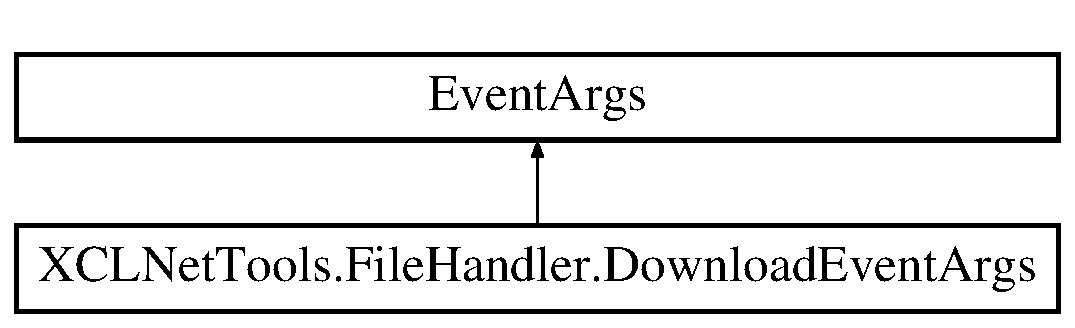
\includegraphics[height=2.000000cm]{class_x_c_l_net_tools_1_1_file_handler_1_1_download_event_args}
\end{center}
\end{figure}
\subsection*{属性}
\begin{DoxyCompactItemize}
\item 
int \hyperlink{class_x_c_l_net_tools_1_1_file_handler_1_1_download_event_args_a1ea772d1ec4b2e0f1f3001fe069bac42}{Bytes\-Received}\hspace{0.3cm}{\ttfamily  \mbox{[}get, set\mbox{]}}
\begin{DoxyCompactList}\small\item\em 已接收的字节数 \end{DoxyCompactList}\item 
int \hyperlink{class_x_c_l_net_tools_1_1_file_handler_1_1_download_event_args_a344cbcca5a213a50ecd25b90340be816}{Total\-Bytes}\hspace{0.3cm}{\ttfamily  \mbox{[}get, set\mbox{]}}
\begin{DoxyCompactList}\small\item\em 总字节数 \end{DoxyCompactList}\item 
byte\mbox{[}$\,$\mbox{]} \hyperlink{class_x_c_l_net_tools_1_1_file_handler_1_1_download_event_args_ae080073b3629650c3befb398e9d7c2e8}{Received\-Data}\hspace{0.3cm}{\ttfamily  \mbox{[}get, set\mbox{]}}
\begin{DoxyCompactList}\small\item\em 当前缓冲区接收的数据 \end{DoxyCompactList}\end{DoxyCompactItemize}


\subsection{详细描述}
下载数据参数 



在文件 Http\-Proc.\-cs 第 66 行定义.



\subsection{属性说明}
\hypertarget{class_x_c_l_net_tools_1_1_file_handler_1_1_download_event_args_a1ea772d1ec4b2e0f1f3001fe069bac42}{\index{X\-C\-L\-Net\-Tools\-::\-File\-Handler\-::\-Download\-Event\-Args@{X\-C\-L\-Net\-Tools\-::\-File\-Handler\-::\-Download\-Event\-Args}!Bytes\-Received@{Bytes\-Received}}
\index{Bytes\-Received@{Bytes\-Received}!XCLNetTools::FileHandler::DownloadEventArgs@{X\-C\-L\-Net\-Tools\-::\-File\-Handler\-::\-Download\-Event\-Args}}
\subsubsection[{Bytes\-Received}]{\setlength{\rightskip}{0pt plus 5cm}int X\-C\-L\-Net\-Tools.\-File\-Handler.\-Download\-Event\-Args.\-Bytes\-Received\hspace{0.3cm}{\ttfamily [get]}, {\ttfamily [set]}}}\label{class_x_c_l_net_tools_1_1_file_handler_1_1_download_event_args_a1ea772d1ec4b2e0f1f3001fe069bac42}


已接收的字节数 



在文件 Http\-Proc.\-cs 第 76 行定义.

\hypertarget{class_x_c_l_net_tools_1_1_file_handler_1_1_download_event_args_ae080073b3629650c3befb398e9d7c2e8}{\index{X\-C\-L\-Net\-Tools\-::\-File\-Handler\-::\-Download\-Event\-Args@{X\-C\-L\-Net\-Tools\-::\-File\-Handler\-::\-Download\-Event\-Args}!Received\-Data@{Received\-Data}}
\index{Received\-Data@{Received\-Data}!XCLNetTools::FileHandler::DownloadEventArgs@{X\-C\-L\-Net\-Tools\-::\-File\-Handler\-::\-Download\-Event\-Args}}
\subsubsection[{Received\-Data}]{\setlength{\rightskip}{0pt plus 5cm}byte \mbox{[}$\,$\mbox{]} X\-C\-L\-Net\-Tools.\-File\-Handler.\-Download\-Event\-Args.\-Received\-Data\hspace{0.3cm}{\ttfamily [get]}, {\ttfamily [set]}}}\label{class_x_c_l_net_tools_1_1_file_handler_1_1_download_event_args_ae080073b3629650c3befb398e9d7c2e8}


当前缓冲区接收的数据 



在文件 Http\-Proc.\-cs 第 94 行定义.

\hypertarget{class_x_c_l_net_tools_1_1_file_handler_1_1_download_event_args_a344cbcca5a213a50ecd25b90340be816}{\index{X\-C\-L\-Net\-Tools\-::\-File\-Handler\-::\-Download\-Event\-Args@{X\-C\-L\-Net\-Tools\-::\-File\-Handler\-::\-Download\-Event\-Args}!Total\-Bytes@{Total\-Bytes}}
\index{Total\-Bytes@{Total\-Bytes}!XCLNetTools::FileHandler::DownloadEventArgs@{X\-C\-L\-Net\-Tools\-::\-File\-Handler\-::\-Download\-Event\-Args}}
\subsubsection[{Total\-Bytes}]{\setlength{\rightskip}{0pt plus 5cm}int X\-C\-L\-Net\-Tools.\-File\-Handler.\-Download\-Event\-Args.\-Total\-Bytes\hspace{0.3cm}{\ttfamily [get]}, {\ttfamily [set]}}}\label{class_x_c_l_net_tools_1_1_file_handler_1_1_download_event_args_a344cbcca5a213a50ecd25b90340be816}


总字节数 



在文件 Http\-Proc.\-cs 第 85 行定义.



该类的文档由以下文件生成\-:\begin{DoxyCompactItemize}
\item 
D\-:/\-My\-Data/\-My\-Git/\-Git\-Hub/\-X\-C\-L\-Net\-Tools/\-X\-C\-L\-Net\-Tools/\-File\-Handler/\hyperlink{_http_proc_8cs}{Http\-Proc.\-cs}\end{DoxyCompactItemize}

\hypertarget{class_x_c_l_net_tools_1_1_enum_1_1_enum_field_model}{\section{X\-C\-L\-Net\-Tools.\-Enum.\-Enum\-Field\-Model类 参考}
\label{class_x_c_l_net_tools_1_1_enum_1_1_enum_field_model}\index{X\-C\-L\-Net\-Tools.\-Enum.\-Enum\-Field\-Model@{X\-C\-L\-Net\-Tools.\-Enum.\-Enum\-Field\-Model}}
}


Enum项model  


\subsection*{属性}
\begin{DoxyCompactItemize}
\item 
string \hyperlink{class_x_c_l_net_tools_1_1_enum_1_1_enum_field_model_acbbc7df1972c0c70dfcf43413da878a8}{Text}\hspace{0.3cm}{\ttfamily  \mbox{[}get, set\mbox{]}}
\begin{DoxyCompactList}\small\item\em text值 \end{DoxyCompactList}\item 
string \hyperlink{class_x_c_l_net_tools_1_1_enum_1_1_enum_field_model_a907462fed405f7065a6fc013cc919e29}{Value}\hspace{0.3cm}{\ttfamily  \mbox{[}get, set\mbox{]}}
\begin{DoxyCompactList}\small\item\em value值 \end{DoxyCompactList}\item 
string \hyperlink{class_x_c_l_net_tools_1_1_enum_1_1_enum_field_model_a182875468bc25ee9c6adb98582e3683e}{Description}\hspace{0.3cm}{\ttfamily  \mbox{[}get, set\mbox{]}}
\begin{DoxyCompactList}\small\item\em description特性 \end{DoxyCompactList}\end{DoxyCompactItemize}


\subsection{详细描述}
Enum项model 



在文件 Enum\-Field\-Model.\-cs 第 30 行定义.



\subsection{属性说明}
\hypertarget{class_x_c_l_net_tools_1_1_enum_1_1_enum_field_model_a182875468bc25ee9c6adb98582e3683e}{\index{X\-C\-L\-Net\-Tools\-::\-Enum\-::\-Enum\-Field\-Model@{X\-C\-L\-Net\-Tools\-::\-Enum\-::\-Enum\-Field\-Model}!Description@{Description}}
\index{Description@{Description}!XCLNetTools::Enum::EnumFieldModel@{X\-C\-L\-Net\-Tools\-::\-Enum\-::\-Enum\-Field\-Model}}
\subsubsection[{Description}]{\setlength{\rightskip}{0pt plus 5cm}string X\-C\-L\-Net\-Tools.\-Enum.\-Enum\-Field\-Model.\-Description\hspace{0.3cm}{\ttfamily [get]}, {\ttfamily [set]}}}\label{class_x_c_l_net_tools_1_1_enum_1_1_enum_field_model_a182875468bc25ee9c6adb98582e3683e}


description特性 



在文件 Enum\-Field\-Model.\-cs 第 45 行定义.

\hypertarget{class_x_c_l_net_tools_1_1_enum_1_1_enum_field_model_acbbc7df1972c0c70dfcf43413da878a8}{\index{X\-C\-L\-Net\-Tools\-::\-Enum\-::\-Enum\-Field\-Model@{X\-C\-L\-Net\-Tools\-::\-Enum\-::\-Enum\-Field\-Model}!Text@{Text}}
\index{Text@{Text}!XCLNetTools::Enum::EnumFieldModel@{X\-C\-L\-Net\-Tools\-::\-Enum\-::\-Enum\-Field\-Model}}
\subsubsection[{Text}]{\setlength{\rightskip}{0pt plus 5cm}string X\-C\-L\-Net\-Tools.\-Enum.\-Enum\-Field\-Model.\-Text\hspace{0.3cm}{\ttfamily [get]}, {\ttfamily [set]}}}\label{class_x_c_l_net_tools_1_1_enum_1_1_enum_field_model_acbbc7df1972c0c70dfcf43413da878a8}


text值 



在文件 Enum\-Field\-Model.\-cs 第 35 行定义.

\hypertarget{class_x_c_l_net_tools_1_1_enum_1_1_enum_field_model_a907462fed405f7065a6fc013cc919e29}{\index{X\-C\-L\-Net\-Tools\-::\-Enum\-::\-Enum\-Field\-Model@{X\-C\-L\-Net\-Tools\-::\-Enum\-::\-Enum\-Field\-Model}!Value@{Value}}
\index{Value@{Value}!XCLNetTools::Enum::EnumFieldModel@{X\-C\-L\-Net\-Tools\-::\-Enum\-::\-Enum\-Field\-Model}}
\subsubsection[{Value}]{\setlength{\rightskip}{0pt plus 5cm}string X\-C\-L\-Net\-Tools.\-Enum.\-Enum\-Field\-Model.\-Value\hspace{0.3cm}{\ttfamily [get]}, {\ttfamily [set]}}}\label{class_x_c_l_net_tools_1_1_enum_1_1_enum_field_model_a907462fed405f7065a6fc013cc919e29}


value值 



在文件 Enum\-Field\-Model.\-cs 第 40 行定义.



该类的文档由以下文件生成\-:\begin{DoxyCompactItemize}
\item 
D\-:/\-My\-Data/\-My\-Git/\-Git\-Hub/\-X\-C\-L\-Net\-Tools/\-X\-C\-L\-Net\-Tools/\-Enum/\hyperlink{_enum_field_model_8cs}{Enum\-Field\-Model.\-cs}\end{DoxyCompactItemize}

\hypertarget{class_x_c_l_net_tools_1_1_enum_1_1_enum_helper}{\section{X\-C\-L\-Net\-Tools.\-Enum.\-Enum\-Helper类 参考}
\label{class_x_c_l_net_tools_1_1_enum_1_1_enum_helper}\index{X\-C\-L\-Net\-Tools.\-Enum.\-Enum\-Helper@{X\-C\-L\-Net\-Tools.\-Enum.\-Enum\-Helper}}
}


枚举帮助类  


\subsection*{静态 Public 成员函数}
\begin{DoxyCompactItemize}
\item 
static List\\*
$<$ \hyperlink{class_x_c_l_net_tools_1_1_entity_1_1_enum_1_1_enum_field_model}{X\-C\-L\-Net\-Tools.\-Entity.\-Enum.\-Enum\-Field\-Model} $>$ \hyperlink{class_x_c_l_net_tools_1_1_enum_1_1_enum_helper_acdcc3f9200705cc0831c1395f5d2c51e}{Get\-Enum\-Field\-Model\-List} (Type em\-Type)
\begin{DoxyCompactList}\small\item\em 将枚举转为\-List(包含自定义属性description)(value为int型的string) 已按枚举的value升序排列 \end{DoxyCompactList}\item 
static List\\*
$<$ X\-C\-L\-Net\-Tools.\-Entity.\-Enum.\-Enum\-Field\-T\-Model\\*
$<$ T $>$ $>$ \hyperlink{class_x_c_l_net_tools_1_1_enum_1_1_enum_helper_a919aa80b589b8038b8db6f731b50556d}{Get\-Enum\-Field\-T\-Model\-List$<$ T $>$} (Type em\-Type)
\begin{DoxyCompactList}\small\item\em 将枚举转为\-List(包含自定义属性description) 已按枚举的value升序排列 \end{DoxyCompactList}\item 
static string \hyperlink{class_x_c_l_net_tools_1_1_enum_1_1_enum_helper_a3445493f9dd4798778af8ecfb2062b1b}{Get\-Enum\-Desc$<$ T $>$} (T enumtype)
\begin{DoxyCompactList}\small\item\em 获取枚举的description注解 \end{DoxyCompactList}\item 
static string \hyperlink{class_x_c_l_net_tools_1_1_enum_1_1_enum_helper_ac1c67f6247644347ed4673965832feaf}{Get\-Enum\-Description\-By\-Text} (Type T, string text)
\begin{DoxyCompactList}\small\item\em 根据枚举text,获取枚举description \end{DoxyCompactList}\item 
static List\\*
$<$ \hyperlink{class_x_c_l_net_tools_1_1_entity_1_1_text_value}{X\-C\-L\-Net\-Tools.\-Entity.\-Text\-Value} $>$ \hyperlink{class_x_c_l_net_tools_1_1_enum_1_1_enum_helper_a0f98e6348aacd00a6254794e6565c173}{Get\-List} (Type type)
\begin{DoxyCompactList}\small\item\em 将枚举转为list的形式 \end{DoxyCompactList}\item 
static bool \hyperlink{class_x_c_l_net_tools_1_1_enum_1_1_enum_helper_a364b52512aee90c0f2530745f4127047}{Is\-Exist\-Enum\-Value} (int v, Type type)
\begin{DoxyCompactList}\small\item\em 判断数字是否属于该枚举 \end{DoxyCompactList}\item 
static int \hyperlink{class_x_c_l_net_tools_1_1_enum_1_1_enum_helper_ab5d340064717d8cf3c9c6036d3770b1f}{Get\-Value\-By\-Text} (List$<$ \hyperlink{class_x_c_l_net_tools_1_1_entity_1_1_text_value}{X\-C\-L\-Net\-Tools.\-Entity.\-Text\-Value} $>$ lst, string text)
\begin{DoxyCompactList}\small\item\em 根据名获取值(若未找到,则返回-\/1) \end{DoxyCompactList}\item 
static int \hyperlink{class_x_c_l_net_tools_1_1_enum_1_1_enum_helper_a8ee641787655d2b4f06cb51486ea8be3}{Get\-Bit\-O\-R\-Value$<$ T $>$} (List$<$ T $>$ em)
\begin{DoxyCompactList}\small\item\em 将多个枚举项进行(按位或)操作,返回int型,若失败,则返回null \end{DoxyCompactList}\item 
static List$<$ T $>$ \hyperlink{class_x_c_l_net_tools_1_1_enum_1_1_enum_helper_a7023c3a9e2c46de0cdeed71bce2cfb6a}{Get\-Enum\-List\-By\-Bit\-Value$<$ T $>$} (int val)
\begin{DoxyCompactList}\small\item\em 根据多个枚举项(按位或)之后的int值,返回枚举list \end{DoxyCompactList}\end{DoxyCompactItemize}


\subsection{详细描述}
枚举帮助类 



在文件 Enum\-Helper.\-cs 第 36 行定义.



\subsection{成员函数说明}
\hypertarget{class_x_c_l_net_tools_1_1_enum_1_1_enum_helper_a8ee641787655d2b4f06cb51486ea8be3}{\index{X\-C\-L\-Net\-Tools\-::\-Enum\-::\-Enum\-Helper@{X\-C\-L\-Net\-Tools\-::\-Enum\-::\-Enum\-Helper}!Get\-Bit\-O\-R\-Value$<$ T $>$@{Get\-Bit\-O\-R\-Value$<$ T $>$}}
\index{Get\-Bit\-O\-R\-Value$<$ T $>$@{Get\-Bit\-O\-R\-Value$<$ T $>$}!XCLNetTools::Enum::EnumHelper@{X\-C\-L\-Net\-Tools\-::\-Enum\-::\-Enum\-Helper}}
\subsubsection[{Get\-Bit\-O\-R\-Value$<$ T $>$}]{\setlength{\rightskip}{0pt plus 5cm}static int X\-C\-L\-Net\-Tools.\-Enum.\-Enum\-Helper.\-Get\-Bit\-O\-R\-Value$<$ T $>$ (
\begin{DoxyParamCaption}
\item[{List$<$ T $>$}]{em}
\end{DoxyParamCaption}
)\hspace{0.3cm}{\ttfamily [static]}}}\label{class_x_c_l_net_tools_1_1_enum_1_1_enum_helper_a8ee641787655d2b4f06cb51486ea8be3}


将多个枚举项进行(按位或)操作,返回int型,若失败,则返回null 

\begin{DoxyReturn}{返回}
结果值
\end{DoxyReturn}


在文件 Enum\-Helper.\-cs 第 219 行定义.

\hypertarget{class_x_c_l_net_tools_1_1_enum_1_1_enum_helper_a3445493f9dd4798778af8ecfb2062b1b}{\index{X\-C\-L\-Net\-Tools\-::\-Enum\-::\-Enum\-Helper@{X\-C\-L\-Net\-Tools\-::\-Enum\-::\-Enum\-Helper}!Get\-Enum\-Desc$<$ T $>$@{Get\-Enum\-Desc$<$ T $>$}}
\index{Get\-Enum\-Desc$<$ T $>$@{Get\-Enum\-Desc$<$ T $>$}!XCLNetTools::Enum::EnumHelper@{X\-C\-L\-Net\-Tools\-::\-Enum\-::\-Enum\-Helper}}
\subsubsection[{Get\-Enum\-Desc$<$ T $>$}]{\setlength{\rightskip}{0pt plus 5cm}static string X\-C\-L\-Net\-Tools.\-Enum.\-Enum\-Helper.\-Get\-Enum\-Desc$<$ T $>$ (
\begin{DoxyParamCaption}
\item[{T}]{enumtype}
\end{DoxyParamCaption}
)\hspace{0.3cm}{\ttfamily [static]}}}\label{class_x_c_l_net_tools_1_1_enum_1_1_enum_helper_a3445493f9dd4798778af8ecfb2062b1b}


获取枚举的description注解 

\begin{DoxyReturn}{返回}
枚举的描述
\end{DoxyReturn}


在文件 Enum\-Helper.\-cs 第 110 行定义.

\hypertarget{class_x_c_l_net_tools_1_1_enum_1_1_enum_helper_ac1c67f6247644347ed4673965832feaf}{\index{X\-C\-L\-Net\-Tools\-::\-Enum\-::\-Enum\-Helper@{X\-C\-L\-Net\-Tools\-::\-Enum\-::\-Enum\-Helper}!Get\-Enum\-Description\-By\-Text@{Get\-Enum\-Description\-By\-Text}}
\index{Get\-Enum\-Description\-By\-Text@{Get\-Enum\-Description\-By\-Text}!XCLNetTools::Enum::EnumHelper@{X\-C\-L\-Net\-Tools\-::\-Enum\-::\-Enum\-Helper}}
\subsubsection[{Get\-Enum\-Description\-By\-Text}]{\setlength{\rightskip}{0pt plus 5cm}static string X\-C\-L\-Net\-Tools.\-Enum.\-Enum\-Helper.\-Get\-Enum\-Description\-By\-Text (
\begin{DoxyParamCaption}
\item[{Type}]{T, }
\item[{string}]{text}
\end{DoxyParamCaption}
)\hspace{0.3cm}{\ttfamily [static]}}}\label{class_x_c_l_net_tools_1_1_enum_1_1_enum_helper_ac1c67f6247644347ed4673965832feaf}


根据枚举text,获取枚举description 

\begin{DoxyReturn}{返回}
枚举的描述
\end{DoxyReturn}


在文件 Enum\-Helper.\-cs 第 137 行定义.

\hypertarget{class_x_c_l_net_tools_1_1_enum_1_1_enum_helper_acdcc3f9200705cc0831c1395f5d2c51e}{\index{X\-C\-L\-Net\-Tools\-::\-Enum\-::\-Enum\-Helper@{X\-C\-L\-Net\-Tools\-::\-Enum\-::\-Enum\-Helper}!Get\-Enum\-Field\-Model\-List@{Get\-Enum\-Field\-Model\-List}}
\index{Get\-Enum\-Field\-Model\-List@{Get\-Enum\-Field\-Model\-List}!XCLNetTools::Enum::EnumHelper@{X\-C\-L\-Net\-Tools\-::\-Enum\-::\-Enum\-Helper}}
\subsubsection[{Get\-Enum\-Field\-Model\-List}]{\setlength{\rightskip}{0pt plus 5cm}static List$<${\bf X\-C\-L\-Net\-Tools.\-Entity.\-Enum.\-Enum\-Field\-Model}$>$ X\-C\-L\-Net\-Tools.\-Enum.\-Enum\-Helper.\-Get\-Enum\-Field\-Model\-List (
\begin{DoxyParamCaption}
\item[{Type}]{em\-Type}
\end{DoxyParamCaption}
)\hspace{0.3cm}{\ttfamily [static]}}}\label{class_x_c_l_net_tools_1_1_enum_1_1_enum_helper_acdcc3f9200705cc0831c1395f5d2c51e}


将枚举转为\-List(包含自定义属性description)(value为int型的string) 已按枚举的value升序排列 


\begin{DoxyParams}{参数}
{\em em\-Type} & 枚举type\\
\hline
\end{DoxyParams}
\begin{DoxyReturn}{返回}
枚举的\-List
\end{DoxyReturn}


在文件 Enum\-Helper.\-cs 第 44 行定义.

\hypertarget{class_x_c_l_net_tools_1_1_enum_1_1_enum_helper_a919aa80b589b8038b8db6f731b50556d}{\index{X\-C\-L\-Net\-Tools\-::\-Enum\-::\-Enum\-Helper@{X\-C\-L\-Net\-Tools\-::\-Enum\-::\-Enum\-Helper}!Get\-Enum\-Field\-T\-Model\-List$<$ T $>$@{Get\-Enum\-Field\-T\-Model\-List$<$ T $>$}}
\index{Get\-Enum\-Field\-T\-Model\-List$<$ T $>$@{Get\-Enum\-Field\-T\-Model\-List$<$ T $>$}!XCLNetTools::Enum::EnumHelper@{X\-C\-L\-Net\-Tools\-::\-Enum\-::\-Enum\-Helper}}
\subsubsection[{Get\-Enum\-Field\-T\-Model\-List$<$ T $>$}]{\setlength{\rightskip}{0pt plus 5cm}static List$<$X\-C\-L\-Net\-Tools.\-Entity.\-Enum.\-Enum\-Field\-T\-Model$<$T$>$ $>$ X\-C\-L\-Net\-Tools.\-Enum.\-Enum\-Helper.\-Get\-Enum\-Field\-T\-Model\-List$<$ T $>$ (
\begin{DoxyParamCaption}
\item[{Type}]{em\-Type}
\end{DoxyParamCaption}
)\hspace{0.3cm}{\ttfamily [static]}}}\label{class_x_c_l_net_tools_1_1_enum_1_1_enum_helper_a919aa80b589b8038b8db6f731b50556d}


将枚举转为\-List(包含自定义属性description) 已按枚举的value升序排列 


\begin{DoxyParams}{参数}
{\em em\-Type} & 枚举type\\
\hline
\end{DoxyParams}

\begin{DoxyTemplParams}{Template Parameters}
{\em T} & 枚举value的类型((可为byte、sbyte、short、ushort、int、uint、long 或 ulong。))\\
\hline
\end{DoxyTemplParams}
\begin{DoxyReturn}{返回}
枚举的\-List
\end{DoxyReturn}


在文件 Enum\-Helper.\-cs 第 71 行定义.

\hypertarget{class_x_c_l_net_tools_1_1_enum_1_1_enum_helper_a7023c3a9e2c46de0cdeed71bce2cfb6a}{\index{X\-C\-L\-Net\-Tools\-::\-Enum\-::\-Enum\-Helper@{X\-C\-L\-Net\-Tools\-::\-Enum\-::\-Enum\-Helper}!Get\-Enum\-List\-By\-Bit\-Value$<$ T $>$@{Get\-Enum\-List\-By\-Bit\-Value$<$ T $>$}}
\index{Get\-Enum\-List\-By\-Bit\-Value$<$ T $>$@{Get\-Enum\-List\-By\-Bit\-Value$<$ T $>$}!XCLNetTools::Enum::EnumHelper@{X\-C\-L\-Net\-Tools\-::\-Enum\-::\-Enum\-Helper}}
\subsubsection[{Get\-Enum\-List\-By\-Bit\-Value$<$ T $>$}]{\setlength{\rightskip}{0pt plus 5cm}static List$<$T$>$ X\-C\-L\-Net\-Tools.\-Enum.\-Enum\-Helper.\-Get\-Enum\-List\-By\-Bit\-Value$<$ T $>$ (
\begin{DoxyParamCaption}
\item[{int}]{val}
\end{DoxyParamCaption}
)\hspace{0.3cm}{\ttfamily [static]}}}\label{class_x_c_l_net_tools_1_1_enum_1_1_enum_helper_a7023c3a9e2c46de0cdeed71bce2cfb6a}


根据多个枚举项(按位或)之后的int值,返回枚举list 

\begin{DoxyReturn}{返回}
枚举list
\end{DoxyReturn}


在文件 Enum\-Helper.\-cs 第 241 行定义.

\hypertarget{class_x_c_l_net_tools_1_1_enum_1_1_enum_helper_a0f98e6348aacd00a6254794e6565c173}{\index{X\-C\-L\-Net\-Tools\-::\-Enum\-::\-Enum\-Helper@{X\-C\-L\-Net\-Tools\-::\-Enum\-::\-Enum\-Helper}!Get\-List@{Get\-List}}
\index{Get\-List@{Get\-List}!XCLNetTools::Enum::EnumHelper@{X\-C\-L\-Net\-Tools\-::\-Enum\-::\-Enum\-Helper}}
\subsubsection[{Get\-List}]{\setlength{\rightskip}{0pt plus 5cm}static List$<${\bf X\-C\-L\-Net\-Tools.\-Entity.\-Text\-Value}$>$ X\-C\-L\-Net\-Tools.\-Enum.\-Enum\-Helper.\-Get\-List (
\begin{DoxyParamCaption}
\item[{Type}]{type}
\end{DoxyParamCaption}
)\hspace{0.3cm}{\ttfamily [static]}}}\label{class_x_c_l_net_tools_1_1_enum_1_1_enum_helper_a0f98e6348aacd00a6254794e6565c173}


将枚举转为list的形式 


\begin{DoxyParams}{参数}
{\em type} & 枚举的typeof\\
\hline
\end{DoxyParams}
\begin{DoxyReturn}{返回}
枚举的list形式
\end{DoxyReturn}


在文件 Enum\-Helper.\-cs 第 153 行定义.

\hypertarget{class_x_c_l_net_tools_1_1_enum_1_1_enum_helper_ab5d340064717d8cf3c9c6036d3770b1f}{\index{X\-C\-L\-Net\-Tools\-::\-Enum\-::\-Enum\-Helper@{X\-C\-L\-Net\-Tools\-::\-Enum\-::\-Enum\-Helper}!Get\-Value\-By\-Text@{Get\-Value\-By\-Text}}
\index{Get\-Value\-By\-Text@{Get\-Value\-By\-Text}!XCLNetTools::Enum::EnumHelper@{X\-C\-L\-Net\-Tools\-::\-Enum\-::\-Enum\-Helper}}
\subsubsection[{Get\-Value\-By\-Text}]{\setlength{\rightskip}{0pt plus 5cm}static int X\-C\-L\-Net\-Tools.\-Enum.\-Enum\-Helper.\-Get\-Value\-By\-Text (
\begin{DoxyParamCaption}
\item[{List$<$ {\bf X\-C\-L\-Net\-Tools.\-Entity.\-Text\-Value} $>$}]{lst, }
\item[{string}]{text}
\end{DoxyParamCaption}
)\hspace{0.3cm}{\ttfamily [static]}}}\label{class_x_c_l_net_tools_1_1_enum_1_1_enum_helper_ab5d340064717d8cf3c9c6036d3770b1f}


根据名获取值(若未找到,则返回-\/1) 


\begin{DoxyParams}{参数}
{\em lst} & 枚举的list形式\\
\hline
{\em text} & 枚举项的名称\\
\hline
\end{DoxyParams}
\begin{DoxyReturn}{返回}
该枚举的值
\end{DoxyReturn}


在文件 Enum\-Helper.\-cs 第 201 行定义.

\hypertarget{class_x_c_l_net_tools_1_1_enum_1_1_enum_helper_a364b52512aee90c0f2530745f4127047}{\index{X\-C\-L\-Net\-Tools\-::\-Enum\-::\-Enum\-Helper@{X\-C\-L\-Net\-Tools\-::\-Enum\-::\-Enum\-Helper}!Is\-Exist\-Enum\-Value@{Is\-Exist\-Enum\-Value}}
\index{Is\-Exist\-Enum\-Value@{Is\-Exist\-Enum\-Value}!XCLNetTools::Enum::EnumHelper@{X\-C\-L\-Net\-Tools\-::\-Enum\-::\-Enum\-Helper}}
\subsubsection[{Is\-Exist\-Enum\-Value}]{\setlength{\rightskip}{0pt plus 5cm}static bool X\-C\-L\-Net\-Tools.\-Enum.\-Enum\-Helper.\-Is\-Exist\-Enum\-Value (
\begin{DoxyParamCaption}
\item[{int}]{v, }
\item[{Type}]{type}
\end{DoxyParamCaption}
)\hspace{0.3cm}{\ttfamily [static]}}}\label{class_x_c_l_net_tools_1_1_enum_1_1_enum_helper_a364b52512aee90c0f2530745f4127047}


判断数字是否属于该枚举 


\begin{DoxyParams}{参数}
{\em v} & 枚举的value,就是数字\\
\hline
{\em type} & 枚举的typeof\\
\hline
\end{DoxyParams}
\begin{DoxyReturn}{返回}
true\-:v属于该枚举,反之则不属于
\end{DoxyReturn}


在文件 Enum\-Helper.\-cs 第 180 行定义.



该类的文档由以下文件生成\-:\begin{DoxyCompactItemize}
\item 
D\-:/\-My\-Data/\-My\-Git/\-Git\-Hub/\-X\-C\-L\-Net\-Tools/\-X\-C\-L\-Net\-Tools/\-Enum/\hyperlink{_enum_helper_8cs}{Enum\-Helper.\-cs}\end{DoxyCompactItemize}

\hypertarget{class_x_c_l_net_tools_1_1_message_1_1_error_1_1_error_http_module}{}\section{X\+C\+L\+Net\+Tools.\+Message.\+Error.\+Error\+Http\+Module类 参考}
\label{class_x_c_l_net_tools_1_1_message_1_1_error_1_1_error_http_module}\index{X\+C\+L\+Net\+Tools.\+Message.\+Error.\+Error\+Http\+Module@{X\+C\+L\+Net\+Tools.\+Message.\+Error.\+Error\+Http\+Module}}


异常处理  


类 X\+C\+L\+Net\+Tools.\+Message.\+Error.\+Error\+Http\+Module 继承关系图\+:\begin{figure}[H]
\begin{center}
\leavevmode
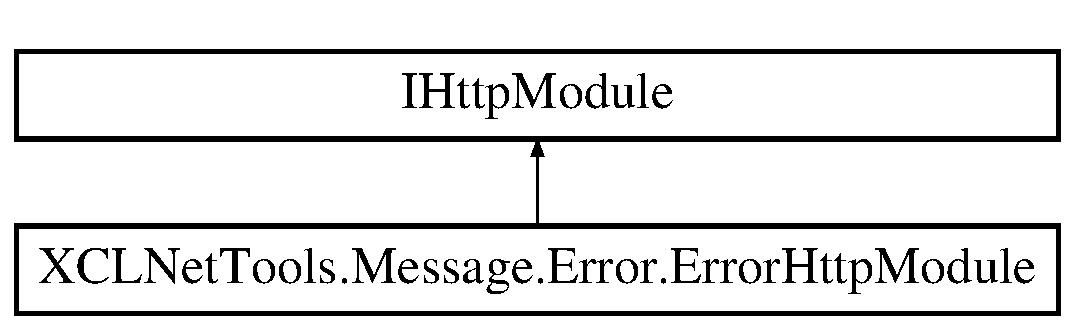
\includegraphics[height=2.000000cm]{class_x_c_l_net_tools_1_1_message_1_1_error_1_1_error_http_module}
\end{center}
\end{figure}
\subsection*{Public 成员函数}
\begin{DoxyCompactItemize}
\item 
void \hyperlink{class_x_c_l_net_tools_1_1_message_1_1_error_1_1_error_http_module_aa4e06d53382795826ed453b62afa265d}{Init} (Http\+Application context)
\begin{DoxyCompactList}\small\item\em 初始化 \end{DoxyCompactList}\item 
void \hyperlink{class_x_c_l_net_tools_1_1_message_1_1_error_1_1_error_http_module_a796d6d747b8620b5e260858e05abd09f}{Dispose} ()
\begin{DoxyCompactList}\small\item\em Dispose \end{DoxyCompactList}\end{DoxyCompactItemize}


\subsection{详细描述}
异常处理 



在文件 Error\+Http\+Module.\+cs 第 18 行定义.



\subsection{成员函数说明}
\mbox{\Hypertarget{class_x_c_l_net_tools_1_1_message_1_1_error_1_1_error_http_module_a796d6d747b8620b5e260858e05abd09f}\label{class_x_c_l_net_tools_1_1_message_1_1_error_1_1_error_http_module_a796d6d747b8620b5e260858e05abd09f}} 
\index{X\+C\+L\+Net\+Tools\+::\+Message\+::\+Error\+::\+Error\+Http\+Module@{X\+C\+L\+Net\+Tools\+::\+Message\+::\+Error\+::\+Error\+Http\+Module}!Dispose@{Dispose}}
\index{Dispose@{Dispose}!X\+C\+L\+Net\+Tools\+::\+Message\+::\+Error\+::\+Error\+Http\+Module@{X\+C\+L\+Net\+Tools\+::\+Message\+::\+Error\+::\+Error\+Http\+Module}}
\subsubsection{\texorpdfstring{Dispose()}{Dispose()}}
{\footnotesize\ttfamily void X\+C\+L\+Net\+Tools.\+Message.\+Error.\+Error\+Http\+Module.\+Dispose (\begin{DoxyParamCaption}{ }\end{DoxyParamCaption})}



Dispose 



在文件 Error\+Http\+Module.\+cs 第 78 行定义.

\mbox{\Hypertarget{class_x_c_l_net_tools_1_1_message_1_1_error_1_1_error_http_module_aa4e06d53382795826ed453b62afa265d}\label{class_x_c_l_net_tools_1_1_message_1_1_error_1_1_error_http_module_aa4e06d53382795826ed453b62afa265d}} 
\index{X\+C\+L\+Net\+Tools\+::\+Message\+::\+Error\+::\+Error\+Http\+Module@{X\+C\+L\+Net\+Tools\+::\+Message\+::\+Error\+::\+Error\+Http\+Module}!Init@{Init}}
\index{Init@{Init}!X\+C\+L\+Net\+Tools\+::\+Message\+::\+Error\+::\+Error\+Http\+Module@{X\+C\+L\+Net\+Tools\+::\+Message\+::\+Error\+::\+Error\+Http\+Module}}
\subsubsection{\texorpdfstring{Init()}{Init()}}
{\footnotesize\ttfamily void X\+C\+L\+Net\+Tools.\+Message.\+Error.\+Error\+Http\+Module.\+Init (\begin{DoxyParamCaption}\item[{Http\+Application}]{context }\end{DoxyParamCaption})}



初始化 



在文件 Error\+Http\+Module.\+cs 第 25 行定义.



该类的文档由以下文件生成\+:\begin{DoxyCompactItemize}
\item 
D\+:/\+My\+Data/\+Git\+Hub/\+X\+C\+L\+Net\+Tools/\+X\+C\+L\+Net\+Tools/\+Message/\+Error/\hyperlink{_error_http_module_8cs}{Error\+Http\+Module.\+cs}\end{DoxyCompactItemize}

\hypertarget{class_x_c_l_net_tools_1_1_data_handler_1_1_excel_helper}{\section{X\-C\-L\-Net\-Tools.\-Data\-Handler.\-Excel\-Helper类 参考}
\label{class_x_c_l_net_tools_1_1_data_handler_1_1_excel_helper}\index{X\-C\-L\-Net\-Tools.\-Data\-Handler.\-Excel\-Helper@{X\-C\-L\-Net\-Tools.\-Data\-Handler.\-Excel\-Helper}}
}


旧版的excel操作(基于excel.\-dll),建议不要使用此类(用aspose.\-cells)  


\subsection*{Public 成员函数}
\begin{DoxyCompactItemize}
\item 
\hyperlink{class_x_c_l_net_tools_1_1_data_handler_1_1_excel_helper_acebffd827fa8842be172440be3e1a134}{Excel\-Helper} (string templet\-File\-Path, string output\-File\-Path)
\begin{DoxyCompactList}\small\item\em 构造函数,将一个已有\-Excel工作簿作为模板,并指定输出路径 \end{DoxyCompactList}\item 
\hyperlink{class_x_c_l_net_tools_1_1_data_handler_1_1_excel_helper_a7b0a4d5a5f8509b97ed054db15ef23d2}{Excel\-Helper} (string file\-Name)
\begin{DoxyCompactList}\small\item\em 构造函数,打开一个已有的工作簿 \end{DoxyCompactList}\item 
\hyperlink{class_x_c_l_net_tools_1_1_data_handler_1_1_excel_helper_a2a3ce10ddfb59e2560a8faa05abc9976}{Excel\-Helper} ()
\begin{DoxyCompactList}\small\item\em 构造函数,新建一个工作簿 \end{DoxyCompactList}\item 
void \hyperlink{class_x_c_l_net_tools_1_1_data_handler_1_1_excel_helper_aee0dd3e95ba5e89b2043cb7d1c969a1c}{Data\-Table\-To\-Excel} (Data\-Table dt, int rows, int top, int left)
\begin{DoxyCompactList}\small\item\em 将\-Data\-Table数据写入\-Excel文件(自动分页) \end{DoxyCompactList}\item 
void \hyperlink{class_x_c_l_net_tools_1_1_data_handler_1_1_excel_helper_a5a62b1a5ff7569e2236ad5eb7a4efcb8}{Data\-Table\-To\-Excel} (Data\-Table dt, int top, int left)
\begin{DoxyCompactList}\small\item\em 将\-Data\-Table数据写入\-Excel文件(不分页) \end{DoxyCompactList}\item 
void \hyperlink{class_x_c_l_net_tools_1_1_data_handler_1_1_excel_helper_a28b1238b8e1008cb4a39ed189df0b73f}{Data\-Table\-To\-Excel} (Data\-Table dt, int rows, int top, int left, int merge\-Column\-Index)
\begin{DoxyCompactList}\small\item\em 将\-Data\-Table数据写入\-Excel文件(自动分页,并指定要合并的列索引) \end{DoxyCompactList}\item 
void \hyperlink{class_x_c_l_net_tools_1_1_data_handler_1_1_excel_helper_a9f6650dba490907278b2ec278f0ecf5d}{Array\-To\-Excel} (string\mbox{[},\mbox{]} arr, int rows, int top, int left)
\begin{DoxyCompactList}\small\item\em 将二维数组数据写入\-Excel文件(自动分页) \end{DoxyCompactList}\item 
void \hyperlink{class_x_c_l_net_tools_1_1_data_handler_1_1_excel_helper_a5be4d665a31a9347e2fe8b3b58b137af}{Array\-To\-Excel} (string\mbox{[},\mbox{]} arr, int top, int left)
\begin{DoxyCompactList}\small\item\em 将二维数组数据写入\-Excel文件(不分页) \end{DoxyCompactList}\item 
void \hyperlink{class_x_c_l_net_tools_1_1_data_handler_1_1_excel_helper_ad2526a27bf44d46c44d8adb56c868c60}{Array\-To\-Excel} (string\mbox{[},\mbox{]} arr, int top, int left, bool is\-Formula)
\begin{DoxyCompactList}\small\item\em 将二维数组数据写入\-Excel文件(不分页) \end{DoxyCompactList}\item 
void \hyperlink{class_x_c_l_net_tools_1_1_data_handler_1_1_excel_helper_a153dfbee4fd21b4ae6eaa1b75955e849}{Array\-To\-Excel} (string\mbox{[},\mbox{]} arr, int top, int left, bool is\-Formula, int merge\-Column\-Index)
\begin{DoxyCompactList}\small\item\em 将二维数组数据写入\-Excel文件(不分页),合并指定列的相同行 \end{DoxyCompactList}\item 
void \hyperlink{class_x_c_l_net_tools_1_1_data_handler_1_1_excel_helper_a7f91871b4a54529f34b3b95fd0c9f0e9}{Array\-To\-Excel} (int sheet\-Index, string\mbox{[},\mbox{]} arr, int top, int left)
\begin{DoxyCompactList}\small\item\em 将二维数组数据写入\-Excel文件(不分页) \end{DoxyCompactList}\item 
void \hyperlink{class_x_c_l_net_tools_1_1_data_handler_1_1_excel_helper_a24dc63cd234dd2bc58a5833b4dcdcc6e}{Array\-To\-Excel} (string\mbox{[},\mbox{]} arr, int rows, int top, int left, int merge\-Column\-Index)
\begin{DoxyCompactList}\small\item\em 将二维数组数据写入\-Excel文件(自动分页,并指定要合并的列索引) \end{DoxyCompactList}\item 
void \hyperlink{class_x_c_l_net_tools_1_1_data_handler_1_1_excel_helper_a5685e97d3cfd67203faeee2bcdd6c788}{Change\-Current\-Work\-Sheet} (int sheet\-Index)
\begin{DoxyCompactList}\small\item\em 改变当前工作表 \end{DoxyCompactList}\item 
void \hyperlink{class_x_c_l_net_tools_1_1_data_handler_1_1_excel_helper_a417d5331a647da31429ff028821e4012}{Hidden\-Work\-Sheet} (string sheet\-Name)
\begin{DoxyCompactList}\small\item\em 隐藏指定名称的工作表 \end{DoxyCompactList}\item 
void \hyperlink{class_x_c_l_net_tools_1_1_data_handler_1_1_excel_helper_a2b65f3492d6d7eeadd2366db1d1cc992}{Hidden\-Work\-Sheet} (int sheet\-Index)
\begin{DoxyCompactList}\small\item\em 隐藏指定索引的工作表 \end{DoxyCompactList}\item 
void \hyperlink{class_x_c_l_net_tools_1_1_data_handler_1_1_excel_helper_a3aa2c1a6e359f9fe7bba76d803ecbb81}{Copy\-Work\-Sheets} (string sheet\-Name, int sheet\-Count)
\begin{DoxyCompactList}\small\item\em 在指定名称的工作表后面拷贝指定个数的该工作表的副本,并重命名 \end{DoxyCompactList}\item 
void \hyperlink{class_x_c_l_net_tools_1_1_data_handler_1_1_excel_helper_a8947f0bbcbbd82566e9083fd30965862}{Copy\-Work\-Sheet} (int src\-Sheet\-Index, int aim\-Sheet\-Index, string new\-Sheet\-Name)
\begin{DoxyCompactList}\small\item\em 将一个工作表拷贝到另一个工作表后面,并重命名 \end{DoxyCompactList}\item 
void \hyperlink{class_x_c_l_net_tools_1_1_data_handler_1_1_excel_helper_ab6b232c0411cec6a15affbe3664a8cd0}{Delete\-Work\-Sheet} (string sheet\-Name)
\begin{DoxyCompactList}\small\item\em 根据名称删除工作表 \end{DoxyCompactList}\item 
void \hyperlink{class_x_c_l_net_tools_1_1_data_handler_1_1_excel_helper_a21db1bb567b78dce9d069f33b22f4b25}{Delete\-Work\-Sheet} (int sheet\-Index)
\begin{DoxyCompactList}\small\item\em 根据索引删除工作表 \end{DoxyCompactList}\item 
void \hyperlink{class_x_c_l_net_tools_1_1_data_handler_1_1_excel_helper_ab8f108b5bd5c60144bc5666884c5191b}{Set\-Text\-Box} (string textbox\-Name, string text)
\begin{DoxyCompactList}\small\item\em 向指定文本框写入数据,对每个\-Work\-Sheet操作 \end{DoxyCompactList}\item 
void \hyperlink{class_x_c_l_net_tools_1_1_data_handler_1_1_excel_helper_a86d566cea97a41b04cad4c896051b6d9}{Set\-Text\-Box} (int sheet\-Index, string textbox\-Name, string text)
\begin{DoxyCompactList}\small\item\em 向指定文本框写入数据,对指定\-Work\-Sheet操作 \end{DoxyCompactList}\item 
void \hyperlink{class_x_c_l_net_tools_1_1_data_handler_1_1_excel_helper_ab9019cd73148e6176ed400ba305d15e5}{Set\-Text\-Boxes} (Hashtable ht)
\begin{DoxyCompactList}\small\item\em 向文本框写入数据,对每个\-Work\-Sheet操作 \end{DoxyCompactList}\item 
void \hyperlink{class_x_c_l_net_tools_1_1_data_handler_1_1_excel_helper_a2b06a36aeacbea3f7158bb45db1f59a2}{Set\-Text\-Boxes} (int sheet\-Index, Hashtable ht)
\begin{DoxyCompactList}\small\item\em 向文本框写入数据,对指定\-Work\-Sheet操作 \end{DoxyCompactList}\item 
void \hyperlink{class_x_c_l_net_tools_1_1_data_handler_1_1_excel_helper_a1210a9f840d18b18bec230c71eb00564}{Set\-Cells} (int row\-Index, int column\-Index, string text)
\begin{DoxyCompactList}\small\item\em 向单元格写入数据,对当前\-Work\-Sheet操作 \end{DoxyCompactList}\item 
void \hyperlink{class_x_c_l_net_tools_1_1_data_handler_1_1_excel_helper_a851825a1eac4c7b8f6644be7ae994bc8}{Set\-Cells} (int sheet\-Index, int row\-Index, int column\-Index, string text)
\begin{DoxyCompactList}\small\item\em 向单元格写入数据,对指定\-Work\-Sheet操作 \end{DoxyCompactList}\item 
void \hyperlink{class_x_c_l_net_tools_1_1_data_handler_1_1_excel_helper_aea03ad91a4cf8544451b8688811a9b26}{Set\-Cells} (Hashtable ht)
\begin{DoxyCompactList}\small\item\em 向单元格写入数据,对每个\-Work\-Sheet操作 \end{DoxyCompactList}\item 
void \hyperlink{class_x_c_l_net_tools_1_1_data_handler_1_1_excel_helper_aa6e6c74debacaac3b04226ca46001829}{Set\-Cells} (int sheet\-Index, Hashtable ht)
\begin{DoxyCompactList}\small\item\em 向单元格写入数据,对指定\-Work\-Sheet操作 \end{DoxyCompactList}\item 
void \hyperlink{class_x_c_l_net_tools_1_1_data_handler_1_1_excel_helper_a66b9b212bd2aec9dc7baf82f7199c362}{Set\-Cells} (int sheet\-Index, string\mbox{[}$\,$\mbox{]} arr)
\begin{DoxyCompactList}\small\item\em 设置单元格为可计算的 \end{DoxyCompactList}\item 
void \hyperlink{class_x_c_l_net_tools_1_1_data_handler_1_1_excel_helper_a95225de93f22b335ddde6d68a3a424e7}{Set\-Cells} (string sheet\-Name, Hashtable ht)
\begin{DoxyCompactList}\small\item\em 向单元格写入数据,对指定\-Work\-Sheet操作 \end{DoxyCompactList}\item 
void \hyperlink{class_x_c_l_net_tools_1_1_data_handler_1_1_excel_helper_ac153094d1d3d435a3f56a673ce95efc1}{Merge\-Cells} (int begin\-Row\-Index, int begin\-Column\-Index, int end\-Row\-Index, int end\-Column\-Index, string text)
\begin{DoxyCompactList}\small\item\em 合并单元格,并赋值,对每个\-Work\-Sheet操作 \end{DoxyCompactList}\item 
void \hyperlink{class_x_c_l_net_tools_1_1_data_handler_1_1_excel_helper_a59d4bebbd2294f88c1d75488330f2d02}{Merge\-Cells} (int sheet\-Index, int begin\-Row\-Index, int begin\-Column\-Index, int end\-Row\-Index, int end\-Column\-Index, string text)
\begin{DoxyCompactList}\small\item\em 合并单元格,并赋值,对指定\-Work\-Sheet操作 \end{DoxyCompactList}\item 
void \hyperlink{class_x_c_l_net_tools_1_1_data_handler_1_1_excel_helper_a6c59b5b2b3b6b38952049c089bdfdf60}{Merge\-Rows} (int column\-Index, int begin\-Row\-Index, int end\-Row\-Index)
\begin{DoxyCompactList}\small\item\em 将指定索引列的数据相同的行合并,对每个\-Work\-Sheet操作 \end{DoxyCompactList}\item 
void \hyperlink{class_x_c_l_net_tools_1_1_data_handler_1_1_excel_helper_a2e506b7e3f336e106a752cbfa3e5329c}{Merge\-Rows} (int sheet\-Index, int column\-Index, int begin\-Row\-Index, int end\-Row\-Index)
\begin{DoxyCompactList}\small\item\em 将指定索引列的数据相同的行合并,对指定\-Work\-Sheet操作 \end{DoxyCompactList}\item 
void \hyperlink{class_x_c_l_net_tools_1_1_data_handler_1_1_excel_helper_a11c7c3f26140bc6f8bfd3f2fee54be60}{Insert\-Rows} (int row\-Index, int count)
\begin{DoxyCompactList}\small\item\em 插行(在指定行上面插入指定数量行) \end{DoxyCompactList}\item 
void \hyperlink{class_x_c_l_net_tools_1_1_data_handler_1_1_excel_helper_a2dda31df749974f5441d442ea21b5183}{Insert\-Rows} (int sheet\-Index, int row\-Index, int count)
\begin{DoxyCompactList}\small\item\em 插行(在指定\-Work\-Sheet指定行上面插入指定数量行) \end{DoxyCompactList}\item 
void \hyperlink{class_x_c_l_net_tools_1_1_data_handler_1_1_excel_helper_a0124826488de4af30d2eaba3fa911500}{Copy\-Rows} (int row\-Index, int count)
\begin{DoxyCompactList}\small\item\em 复制行(在指定行下面复制指定数量行) \end{DoxyCompactList}\item 
void \hyperlink{class_x_c_l_net_tools_1_1_data_handler_1_1_excel_helper_a40281cf4653e2a362aa4e897001ff001}{Copy\-Rows} (int sheet\-Index, int row\-Index, int count)
\begin{DoxyCompactList}\small\item\em 复制行(在指定\-Work\-Sheet指定行下面复制指定数量行) \end{DoxyCompactList}\item 
void \hyperlink{class_x_c_l_net_tools_1_1_data_handler_1_1_excel_helper_a998f8178efe9f0602f1e3d30e9096eb8}{Delete\-Rows} (int row\-Index, int count)
\begin{DoxyCompactList}\small\item\em 删除行 \end{DoxyCompactList}\item 
void \hyperlink{class_x_c_l_net_tools_1_1_data_handler_1_1_excel_helper_aaac48849297e93e10a6ccd8dd30cdd64}{Delete\-Rows} (int sheet\-Index, int row\-Index, int count)
\begin{DoxyCompactList}\small\item\em 删除行 \end{DoxyCompactList}\item 
void \hyperlink{class_x_c_l_net_tools_1_1_data_handler_1_1_excel_helper_a950e53c43178294b31ad227251f5dfcb}{Insert\-Columns} (int column\-Index, int count)
\begin{DoxyCompactList}\small\item\em 插列(在指定列右边插入指定数量列) \end{DoxyCompactList}\item 
void \hyperlink{class_x_c_l_net_tools_1_1_data_handler_1_1_excel_helper_ad5b4582fcf63403a838d9c0b9acd9ee4}{Insert\-Columns} (int sheet\-Index, int column\-Index, int count)
\begin{DoxyCompactList}\small\item\em 插列(在指定\-Work\-Sheet指定列右边插入指定数量列) \end{DoxyCompactList}\item 
void \hyperlink{class_x_c_l_net_tools_1_1_data_handler_1_1_excel_helper_a477309c8e46fd02109a7ee4a8164221d}{Copy\-Columns} (int column\-Index, int count)
\begin{DoxyCompactList}\small\item\em 复制列(在指定列右边复制指定数量列) \end{DoxyCompactList}\item 
void \hyperlink{class_x_c_l_net_tools_1_1_data_handler_1_1_excel_helper_a4747b28517aaa00ebd20abfceb7a8161}{Copy\-Columns} (int sheet\-Index, int column\-Index, int count)
\begin{DoxyCompactList}\small\item\em 复制列(在指定\-Work\-Sheet指定列右边复制指定数量列) \end{DoxyCompactList}\item 
void \hyperlink{class_x_c_l_net_tools_1_1_data_handler_1_1_excel_helper_a07bf346a96fdd9723478313b7bca25e0}{Delete\-Columns} (int column\-Index, int count)
\begin{DoxyCompactList}\small\item\em 删除列 \end{DoxyCompactList}\item 
void \hyperlink{class_x_c_l_net_tools_1_1_data_handler_1_1_excel_helper_a905fec84987bc88a0b28e70f954ca0ea}{Delete\-Columns} (int sheet\-Index, int column\-Index, int count)
\begin{DoxyCompactList}\small\item\em 删除列 \end{DoxyCompactList}\item 
void \hyperlink{class_x_c_l_net_tools_1_1_data_handler_1_1_excel_helper_a383ca6f7c7ad61c7c042ce533153ec87}{Range\-Copy} (int sheet\-Index, string start\-Cell, string end\-Cell, string target\-Cell)
\begin{DoxyCompactList}\small\item\em 将指定范围区域拷贝到目标区域 \end{DoxyCompactList}\item 
void \hyperlink{class_x_c_l_net_tools_1_1_data_handler_1_1_excel_helper_ac81856c1c2e61c5674448c5588d6f88b}{Range\-Copy} (string sheet\-Name, string start\-Cell, string end\-Cell, string target\-Cell)
\begin{DoxyCompactList}\small\item\em 将指定范围区域拷贝到目标区域 \end{DoxyCompactList}\item 
void \hyperlink{class_x_c_l_net_tools_1_1_data_handler_1_1_excel_helper_ab1974e3579c233eb2a8c1b1bcbbc0aea}{Rang\-Auto\-Fill} ()
\begin{DoxyCompactList}\small\item\em 自动填充 \end{DoxyCompactList}\item 
void \hyperlink{class_x_c_l_net_tools_1_1_data_handler_1_1_excel_helper_abc029180bf2199f182a4c60d3a0f585b}{Apply\-Style} ()
\begin{DoxyCompactList}\small\item\em 应用样式 \end{DoxyCompactList}\item 
int \hyperlink{class_x_c_l_net_tools_1_1_data_handler_1_1_excel_helper_a32cace260b279a4fd6861e2925a2bbce}{Letter\-To\-Int} (string letter)
\begin{DoxyCompactList}\small\item\em 将\-Excel列的字母索引值转换成整数索引值 \end{DoxyCompactList}\item 
string \hyperlink{class_x_c_l_net_tools_1_1_data_handler_1_1_excel_helper_a69fec6dfa4e2714e3faeaa88ad92edce}{Int\-To\-Letter} (int n)
\begin{DoxyCompactList}\small\item\em 将\-Excel列的整数索引值转换为字符索引值 \end{DoxyCompactList}\item 
void \hyperlink{class_x_c_l_net_tools_1_1_data_handler_1_1_excel_helper_ad33804b2e7c24ec683fb5db86db433a3}{Output\-Excel\-File} ()
\begin{DoxyCompactList}\small\item\em 输出\-Excel文件并退出 \end{DoxyCompactList}\item 
void \hyperlink{class_x_c_l_net_tools_1_1_data_handler_1_1_excel_helper_a016cbd751ac63913cb80fe03c1870a4b}{Output\-File} (string format)
\begin{DoxyCompactList}\small\item\em 输出指定格式的文件(支持格式:\-H\-T\-M\-L,\-C\-S\-V,\-T\-E\-X\-T,\-E\-X\-C\-E\-L) \end{DoxyCompactList}\item 
void \hyperlink{class_x_c_l_net_tools_1_1_data_handler_1_1_excel_helper_aa009952e56f61cb90529bf2e68b4098b}{Save\-File} ()
\begin{DoxyCompactList}\small\item\em 保存文件 \end{DoxyCompactList}\item 
void \hyperlink{class_x_c_l_net_tools_1_1_data_handler_1_1_excel_helper_ac15d18695f8bcfb21ee446edbd173eb2}{Save\-As\-File} ()
\begin{DoxyCompactList}\small\item\em 另存文件 \end{DoxyCompactList}\item 
void \hyperlink{class_x_c_l_net_tools_1_1_data_handler_1_1_excel_helper_a70b84e514fca4175d6e78e8845b34753}{Save\-As\-File} (string format)
\begin{DoxyCompactList}\small\item\em 将\-Excel文件另存为指定格式 \end{DoxyCompactList}\item 
void \hyperlink{class_x_c_l_net_tools_1_1_data_handler_1_1_excel_helper_a7c3372f5c5fc327080f3b35d85ee4c39}{Save\-File} (string file\-Name)
\begin{DoxyCompactList}\small\item\em 另存文件 \end{DoxyCompactList}\item 
void \hyperlink{class_x_c_l_net_tools_1_1_data_handler_1_1_excel_helper_a401a9ce1828e68dd716bfa13f2e4d9f1}{Save\-As\-File} (string file\-Name, string format)
\begin{DoxyCompactList}\small\item\em 将\-Excel文件另存为指定格式 \end{DoxyCompactList}\item 
int \hyperlink{class_x_c_l_net_tools_1_1_data_handler_1_1_excel_helper_af0a259184ab65d03bd80395f273d1016}{Get\-Sheet\-Count} (int row\-Count, int rows)
\begin{DoxyCompactList}\small\item\em 计算\-Work\-Sheet数量 \end{DoxyCompactList}\item 
void \hyperlink{class_x_c_l_net_tools_1_1_data_handler_1_1_excel_helper_aed272e9ef2e170dadd73a8e7d761b8cd}{Kill\-Excel\-Process} ()
\begin{DoxyCompactList}\small\item\em 结束\-Excel进程 \end{DoxyCompactList}\end{DoxyCompactItemize}
\subsection*{属性}
\begin{DoxyCompactItemize}
\item 
string \hyperlink{class_x_c_l_net_tools_1_1_data_handler_1_1_excel_helper_a19d5234b9309942b87041f70bef91647}{Sheet\-Prefix\-Name}\hspace{0.3cm}{\ttfamily  \mbox{[}set\mbox{]}}
\begin{DoxyCompactList}\small\item\em Work\-Sheet前缀名,比如:前缀名为“页”,那么\-Work\-Sheet名称依次为“页-\/1,页-\/2...” \end{DoxyCompactList}\item 
int \hyperlink{class_x_c_l_net_tools_1_1_data_handler_1_1_excel_helper_ab8d2677869ff64e25bbe54623ef9fa86}{Work\-Sheet\-Count}\hspace{0.3cm}{\ttfamily  \mbox{[}get\mbox{]}}
\begin{DoxyCompactList}\small\item\em Work\-Sheet数量 \end{DoxyCompactList}\item 
string \hyperlink{class_x_c_l_net_tools_1_1_data_handler_1_1_excel_helper_a0e4501c60ef6446d0fe8151a6e58fca4}{Templet\-File\-Path}\hspace{0.3cm}{\ttfamily  \mbox{[}set\mbox{]}}
\begin{DoxyCompactList}\small\item\em Excel模板文件路径 \end{DoxyCompactList}\item 
string \hyperlink{class_x_c_l_net_tools_1_1_data_handler_1_1_excel_helper_ada3dfa77cf3ac278ee83281f04707aa3}{Output\-File\-Path}\hspace{0.3cm}{\ttfamily  \mbox{[}set\mbox{]}}
\begin{DoxyCompactList}\small\item\em 输出\-Excel文件路径 \end{DoxyCompactList}\end{DoxyCompactItemize}


\subsection{详细描述}
旧版的excel操作(基于excel.\-dll),建议不要使用此类(用aspose.\-cells) 



在文件 Excel\-Helper.\-cs 第 13 行定义.



\subsection{构造及析构函数说明}
\hypertarget{class_x_c_l_net_tools_1_1_data_handler_1_1_excel_helper_acebffd827fa8842be172440be3e1a134}{\index{X\-C\-L\-Net\-Tools\-::\-Data\-Handler\-::\-Excel\-Helper@{X\-C\-L\-Net\-Tools\-::\-Data\-Handler\-::\-Excel\-Helper}!Excel\-Helper@{Excel\-Helper}}
\index{Excel\-Helper@{Excel\-Helper}!XCLNetTools::DataHandler::ExcelHelper@{X\-C\-L\-Net\-Tools\-::\-Data\-Handler\-::\-Excel\-Helper}}
\subsubsection[{Excel\-Helper}]{\setlength{\rightskip}{0pt plus 5cm}X\-C\-L\-Net\-Tools.\-Data\-Handler.\-Excel\-Helper.\-Excel\-Helper (
\begin{DoxyParamCaption}
\item[{string}]{templet\-File\-Path, }
\item[{string}]{output\-File\-Path}
\end{DoxyParamCaption}
)}}\label{class_x_c_l_net_tools_1_1_data_handler_1_1_excel_helper_acebffd827fa8842be172440be3e1a134}


构造函数,将一个已有\-Excel工作簿作为模板,并指定输出路径 


\begin{DoxyParams}{参数}
{\em templet\-File\-Path} & Excel模板文件路径\\
\hline
{\em output\-File\-Path} & 输出\-Excel文件路径\\
\hline
\end{DoxyParams}


在文件 Excel\-Helper.\-cs 第 79 行定义.

\hypertarget{class_x_c_l_net_tools_1_1_data_handler_1_1_excel_helper_a7b0a4d5a5f8509b97ed054db15ef23d2}{\index{X\-C\-L\-Net\-Tools\-::\-Data\-Handler\-::\-Excel\-Helper@{X\-C\-L\-Net\-Tools\-::\-Data\-Handler\-::\-Excel\-Helper}!Excel\-Helper@{Excel\-Helper}}
\index{Excel\-Helper@{Excel\-Helper}!XCLNetTools::DataHandler::ExcelHelper@{X\-C\-L\-Net\-Tools\-::\-Data\-Handler\-::\-Excel\-Helper}}
\subsubsection[{Excel\-Helper}]{\setlength{\rightskip}{0pt plus 5cm}X\-C\-L\-Net\-Tools.\-Data\-Handler.\-Excel\-Helper.\-Excel\-Helper (
\begin{DoxyParamCaption}
\item[{string}]{file\-Name}
\end{DoxyParamCaption}
)}}\label{class_x_c_l_net_tools_1_1_data_handler_1_1_excel_helper_a7b0a4d5a5f8509b97ed054db15ef23d2}


构造函数,打开一个已有的工作簿 


\begin{DoxyParams}{参数}
{\em file\-Name} & Excel文件名\\
\hline
\end{DoxyParams}


在文件 Excel\-Helper.\-cs 第 111 行定义.

\hypertarget{class_x_c_l_net_tools_1_1_data_handler_1_1_excel_helper_a2a3ce10ddfb59e2560a8faa05abc9976}{\index{X\-C\-L\-Net\-Tools\-::\-Data\-Handler\-::\-Excel\-Helper@{X\-C\-L\-Net\-Tools\-::\-Data\-Handler\-::\-Excel\-Helper}!Excel\-Helper@{Excel\-Helper}}
\index{Excel\-Helper@{Excel\-Helper}!XCLNetTools::DataHandler::ExcelHelper@{X\-C\-L\-Net\-Tools\-::\-Data\-Handler\-::\-Excel\-Helper}}
\subsubsection[{Excel\-Helper}]{\setlength{\rightskip}{0pt plus 5cm}X\-C\-L\-Net\-Tools.\-Data\-Handler.\-Excel\-Helper.\-Excel\-Helper (
\begin{DoxyParamCaption}
{}
\end{DoxyParamCaption}
)}}\label{class_x_c_l_net_tools_1_1_data_handler_1_1_excel_helper_a2a3ce10ddfb59e2560a8faa05abc9976}


构造函数,新建一个工作簿 



在文件 Excel\-Helper.\-cs 第 135 行定义.



\subsection{成员函数说明}
\hypertarget{class_x_c_l_net_tools_1_1_data_handler_1_1_excel_helper_abc029180bf2199f182a4c60d3a0f585b}{\index{X\-C\-L\-Net\-Tools\-::\-Data\-Handler\-::\-Excel\-Helper@{X\-C\-L\-Net\-Tools\-::\-Data\-Handler\-::\-Excel\-Helper}!Apply\-Style@{Apply\-Style}}
\index{Apply\-Style@{Apply\-Style}!XCLNetTools::DataHandler::ExcelHelper@{X\-C\-L\-Net\-Tools\-::\-Data\-Handler\-::\-Excel\-Helper}}
\subsubsection[{Apply\-Style}]{\setlength{\rightskip}{0pt plus 5cm}void X\-C\-L\-Net\-Tools.\-Data\-Handler.\-Excel\-Helper.\-Apply\-Style (
\begin{DoxyParamCaption}
{}
\end{DoxyParamCaption}
)}}\label{class_x_c_l_net_tools_1_1_data_handler_1_1_excel_helper_abc029180bf2199f182a4c60d3a0f585b}


应用样式 



在文件 Excel\-Helper.\-cs 第 1722 行定义.

\hypertarget{class_x_c_l_net_tools_1_1_data_handler_1_1_excel_helper_a9f6650dba490907278b2ec278f0ecf5d}{\index{X\-C\-L\-Net\-Tools\-::\-Data\-Handler\-::\-Excel\-Helper@{X\-C\-L\-Net\-Tools\-::\-Data\-Handler\-::\-Excel\-Helper}!Array\-To\-Excel@{Array\-To\-Excel}}
\index{Array\-To\-Excel@{Array\-To\-Excel}!XCLNetTools::DataHandler::ExcelHelper@{X\-C\-L\-Net\-Tools\-::\-Data\-Handler\-::\-Excel\-Helper}}
\subsubsection[{Array\-To\-Excel}]{\setlength{\rightskip}{0pt plus 5cm}void X\-C\-L\-Net\-Tools.\-Data\-Handler.\-Excel\-Helper.\-Array\-To\-Excel (
\begin{DoxyParamCaption}
\item[{string}]{arr\mbox{[},\mbox{]}, }
\item[{int}]{rows, }
\item[{int}]{top, }
\item[{int}]{left}
\end{DoxyParamCaption}
)}}\label{class_x_c_l_net_tools_1_1_data_handler_1_1_excel_helper_a9f6650dba490907278b2ec278f0ecf5d}


将二维数组数据写入\-Excel文件(自动分页) 


\begin{DoxyParams}{参数}
{\em arr} & 二维数组\\
\hline
{\em rows} & 每个\-Work\-Sheet写入多少行数据\\
\hline
{\em top} & 行索引\\
\hline
{\em left} & 列索引\\
\hline
\end{DoxyParams}


在文件 Excel\-Helper.\-cs 第 340 行定义.

\hypertarget{class_x_c_l_net_tools_1_1_data_handler_1_1_excel_helper_a5be4d665a31a9347e2fe8b3b58b137af}{\index{X\-C\-L\-Net\-Tools\-::\-Data\-Handler\-::\-Excel\-Helper@{X\-C\-L\-Net\-Tools\-::\-Data\-Handler\-::\-Excel\-Helper}!Array\-To\-Excel@{Array\-To\-Excel}}
\index{Array\-To\-Excel@{Array\-To\-Excel}!XCLNetTools::DataHandler::ExcelHelper@{X\-C\-L\-Net\-Tools\-::\-Data\-Handler\-::\-Excel\-Helper}}
\subsubsection[{Array\-To\-Excel}]{\setlength{\rightskip}{0pt plus 5cm}void X\-C\-L\-Net\-Tools.\-Data\-Handler.\-Excel\-Helper.\-Array\-To\-Excel (
\begin{DoxyParamCaption}
\item[{string}]{arr\mbox{[},\mbox{]}, }
\item[{int}]{top, }
\item[{int}]{left}
\end{DoxyParamCaption}
)}}\label{class_x_c_l_net_tools_1_1_data_handler_1_1_excel_helper_a5be4d665a31a9347e2fe8b3b58b137af}


将二维数组数据写入\-Excel文件(不分页) 


\begin{DoxyParams}{参数}
{\em arr} & 二维数组\\
\hline
{\em top} & 行索引\\
\hline
{\em left} & 列索引\\
\hline
\end{DoxyParams}


在文件 Excel\-Helper.\-cs 第 400 行定义.

\hypertarget{class_x_c_l_net_tools_1_1_data_handler_1_1_excel_helper_ad2526a27bf44d46c44d8adb56c868c60}{\index{X\-C\-L\-Net\-Tools\-::\-Data\-Handler\-::\-Excel\-Helper@{X\-C\-L\-Net\-Tools\-::\-Data\-Handler\-::\-Excel\-Helper}!Array\-To\-Excel@{Array\-To\-Excel}}
\index{Array\-To\-Excel@{Array\-To\-Excel}!XCLNetTools::DataHandler::ExcelHelper@{X\-C\-L\-Net\-Tools\-::\-Data\-Handler\-::\-Excel\-Helper}}
\subsubsection[{Array\-To\-Excel}]{\setlength{\rightskip}{0pt plus 5cm}void X\-C\-L\-Net\-Tools.\-Data\-Handler.\-Excel\-Helper.\-Array\-To\-Excel (
\begin{DoxyParamCaption}
\item[{string}]{arr\mbox{[},\mbox{]}, }
\item[{int}]{top, }
\item[{int}]{left, }
\item[{bool}]{is\-Formula}
\end{DoxyParamCaption}
)}}\label{class_x_c_l_net_tools_1_1_data_handler_1_1_excel_helper_ad2526a27bf44d46c44d8adb56c868c60}


将二维数组数据写入\-Excel文件(不分页) 


\begin{DoxyParams}{参数}
{\em arr} & 二维数组\\
\hline
{\em top} & 行索引\\
\hline
{\em left} & 列索引\\
\hline
{\em is\-Formula} & 填充的数据是否需要计算\\
\hline
\end{DoxyParams}


在文件 Excel\-Helper.\-cs 第 417 行定义.

\hypertarget{class_x_c_l_net_tools_1_1_data_handler_1_1_excel_helper_a153dfbee4fd21b4ae6eaa1b75955e849}{\index{X\-C\-L\-Net\-Tools\-::\-Data\-Handler\-::\-Excel\-Helper@{X\-C\-L\-Net\-Tools\-::\-Data\-Handler\-::\-Excel\-Helper}!Array\-To\-Excel@{Array\-To\-Excel}}
\index{Array\-To\-Excel@{Array\-To\-Excel}!XCLNetTools::DataHandler::ExcelHelper@{X\-C\-L\-Net\-Tools\-::\-Data\-Handler\-::\-Excel\-Helper}}
\subsubsection[{Array\-To\-Excel}]{\setlength{\rightskip}{0pt plus 5cm}void X\-C\-L\-Net\-Tools.\-Data\-Handler.\-Excel\-Helper.\-Array\-To\-Excel (
\begin{DoxyParamCaption}
\item[{string}]{arr\mbox{[},\mbox{]}, }
\item[{int}]{top, }
\item[{int}]{left, }
\item[{bool}]{is\-Formula, }
\item[{int}]{merge\-Column\-Index}
\end{DoxyParamCaption}
)}}\label{class_x_c_l_net_tools_1_1_data_handler_1_1_excel_helper_a153dfbee4fd21b4ae6eaa1b75955e849}


将二维数组数据写入\-Excel文件(不分页),合并指定列的相同行 


\begin{DoxyParams}{参数}
{\em arr} & 二维数组\\
\hline
{\em top} & 行索引\\
\hline
{\em left} & 列索引\\
\hline
{\em is\-Formula} & 填充的数据是否需要计算\\
\hline
{\em merge\-Column\-Index} & 需要合并行的列索引\\
\hline
\end{DoxyParams}


在文件 Excel\-Helper.\-cs 第 440 行定义.

\hypertarget{class_x_c_l_net_tools_1_1_data_handler_1_1_excel_helper_a7f91871b4a54529f34b3b95fd0c9f0e9}{\index{X\-C\-L\-Net\-Tools\-::\-Data\-Handler\-::\-Excel\-Helper@{X\-C\-L\-Net\-Tools\-::\-Data\-Handler\-::\-Excel\-Helper}!Array\-To\-Excel@{Array\-To\-Excel}}
\index{Array\-To\-Excel@{Array\-To\-Excel}!XCLNetTools::DataHandler::ExcelHelper@{X\-C\-L\-Net\-Tools\-::\-Data\-Handler\-::\-Excel\-Helper}}
\subsubsection[{Array\-To\-Excel}]{\setlength{\rightskip}{0pt plus 5cm}void X\-C\-L\-Net\-Tools.\-Data\-Handler.\-Excel\-Helper.\-Array\-To\-Excel (
\begin{DoxyParamCaption}
\item[{int}]{sheet\-Index, }
\item[{string}]{arr\mbox{[},\mbox{]}, }
\item[{int}]{top, }
\item[{int}]{left}
\end{DoxyParamCaption}
)}}\label{class_x_c_l_net_tools_1_1_data_handler_1_1_excel_helper_a7f91871b4a54529f34b3b95fd0c9f0e9}


将二维数组数据写入\-Excel文件(不分页) 


\begin{DoxyParams}{参数}
{\em sheet\-Index} & 工作表索引\\
\hline
{\em arr} & 二维数组\\
\hline
{\em top} & 行索引\\
\hline
{\em left} & 列索引\\
\hline
\end{DoxyParams}


在文件 Excel\-Helper.\-cs 第 464 行定义.

\hypertarget{class_x_c_l_net_tools_1_1_data_handler_1_1_excel_helper_a24dc63cd234dd2bc58a5833b4dcdcc6e}{\index{X\-C\-L\-Net\-Tools\-::\-Data\-Handler\-::\-Excel\-Helper@{X\-C\-L\-Net\-Tools\-::\-Data\-Handler\-::\-Excel\-Helper}!Array\-To\-Excel@{Array\-To\-Excel}}
\index{Array\-To\-Excel@{Array\-To\-Excel}!XCLNetTools::DataHandler::ExcelHelper@{X\-C\-L\-Net\-Tools\-::\-Data\-Handler\-::\-Excel\-Helper}}
\subsubsection[{Array\-To\-Excel}]{\setlength{\rightskip}{0pt plus 5cm}void X\-C\-L\-Net\-Tools.\-Data\-Handler.\-Excel\-Helper.\-Array\-To\-Excel (
\begin{DoxyParamCaption}
\item[{string}]{arr\mbox{[},\mbox{]}, }
\item[{int}]{rows, }
\item[{int}]{top, }
\item[{int}]{left, }
\item[{int}]{merge\-Column\-Index}
\end{DoxyParamCaption}
)}}\label{class_x_c_l_net_tools_1_1_data_handler_1_1_excel_helper_a24dc63cd234dd2bc58a5833b4dcdcc6e}


将二维数组数据写入\-Excel文件(自动分页,并指定要合并的列索引) 


\begin{DoxyParams}{参数}
{\em arr} & 二维数组\\
\hline
{\em rows} & 每个\-Work\-Sheet写入多少行数据\\
\hline
{\em top} & 行索引\\
\hline
{\em left} & 列索引\\
\hline
{\em merge\-Column\-Index} & 数组的二维索引,相当于\-Data\-Table的列索引,索引从0开始\\
\hline
\end{DoxyParams}


在文件 Excel\-Helper.\-cs 第 492 行定义.

\hypertarget{class_x_c_l_net_tools_1_1_data_handler_1_1_excel_helper_a5685e97d3cfd67203faeee2bcdd6c788}{\index{X\-C\-L\-Net\-Tools\-::\-Data\-Handler\-::\-Excel\-Helper@{X\-C\-L\-Net\-Tools\-::\-Data\-Handler\-::\-Excel\-Helper}!Change\-Current\-Work\-Sheet@{Change\-Current\-Work\-Sheet}}
\index{Change\-Current\-Work\-Sheet@{Change\-Current\-Work\-Sheet}!XCLNetTools::DataHandler::ExcelHelper@{X\-C\-L\-Net\-Tools\-::\-Data\-Handler\-::\-Excel\-Helper}}
\subsubsection[{Change\-Current\-Work\-Sheet}]{\setlength{\rightskip}{0pt plus 5cm}void X\-C\-L\-Net\-Tools.\-Data\-Handler.\-Excel\-Helper.\-Change\-Current\-Work\-Sheet (
\begin{DoxyParamCaption}
\item[{int}]{sheet\-Index}
\end{DoxyParamCaption}
)}}\label{class_x_c_l_net_tools_1_1_data_handler_1_1_excel_helper_a5685e97d3cfd67203faeee2bcdd6c788}


改变当前工作表 


\begin{DoxyParams}{参数}
{\em sheet\-Index} & 工作表索引\\
\hline
\end{DoxyParams}


在文件 Excel\-Helper.\-cs 第 557 行定义.

\hypertarget{class_x_c_l_net_tools_1_1_data_handler_1_1_excel_helper_a477309c8e46fd02109a7ee4a8164221d}{\index{X\-C\-L\-Net\-Tools\-::\-Data\-Handler\-::\-Excel\-Helper@{X\-C\-L\-Net\-Tools\-::\-Data\-Handler\-::\-Excel\-Helper}!Copy\-Columns@{Copy\-Columns}}
\index{Copy\-Columns@{Copy\-Columns}!XCLNetTools::DataHandler::ExcelHelper@{X\-C\-L\-Net\-Tools\-::\-Data\-Handler\-::\-Excel\-Helper}}
\subsubsection[{Copy\-Columns}]{\setlength{\rightskip}{0pt plus 5cm}void X\-C\-L\-Net\-Tools.\-Data\-Handler.\-Excel\-Helper.\-Copy\-Columns (
\begin{DoxyParamCaption}
\item[{int}]{column\-Index, }
\item[{int}]{count}
\end{DoxyParamCaption}
)}}\label{class_x_c_l_net_tools_1_1_data_handler_1_1_excel_helper_a477309c8e46fd02109a7ee4a8164221d}


复制列(在指定列右边复制指定数量列) 


\begin{DoxyParams}{参数}
{\em column\-Index} & \\
\hline
{\em count} & \\
\hline
\end{DoxyParams}


在文件 Excel\-Helper.\-cs 第 1493 行定义.

\hypertarget{class_x_c_l_net_tools_1_1_data_handler_1_1_excel_helper_a4747b28517aaa00ebd20abfceb7a8161}{\index{X\-C\-L\-Net\-Tools\-::\-Data\-Handler\-::\-Excel\-Helper@{X\-C\-L\-Net\-Tools\-::\-Data\-Handler\-::\-Excel\-Helper}!Copy\-Columns@{Copy\-Columns}}
\index{Copy\-Columns@{Copy\-Columns}!XCLNetTools::DataHandler::ExcelHelper@{X\-C\-L\-Net\-Tools\-::\-Data\-Handler\-::\-Excel\-Helper}}
\subsubsection[{Copy\-Columns}]{\setlength{\rightskip}{0pt plus 5cm}void X\-C\-L\-Net\-Tools.\-Data\-Handler.\-Excel\-Helper.\-Copy\-Columns (
\begin{DoxyParamCaption}
\item[{int}]{sheet\-Index, }
\item[{int}]{column\-Index, }
\item[{int}]{count}
\end{DoxyParamCaption}
)}}\label{class_x_c_l_net_tools_1_1_data_handler_1_1_excel_helper_a4747b28517aaa00ebd20abfceb7a8161}


复制列(在指定\-Work\-Sheet指定列右边复制指定数量列) 


\begin{DoxyParams}{参数}
{\em sheet\-Index} & \\
\hline
{\em column\-Index} & \\
\hline
{\em count} & \\
\hline
\end{DoxyParams}


在文件 Excel\-Helper.\-cs 第 1524 行定义.

\hypertarget{class_x_c_l_net_tools_1_1_data_handler_1_1_excel_helper_a0124826488de4af30d2eaba3fa911500}{\index{X\-C\-L\-Net\-Tools\-::\-Data\-Handler\-::\-Excel\-Helper@{X\-C\-L\-Net\-Tools\-::\-Data\-Handler\-::\-Excel\-Helper}!Copy\-Rows@{Copy\-Rows}}
\index{Copy\-Rows@{Copy\-Rows}!XCLNetTools::DataHandler::ExcelHelper@{X\-C\-L\-Net\-Tools\-::\-Data\-Handler\-::\-Excel\-Helper}}
\subsubsection[{Copy\-Rows}]{\setlength{\rightskip}{0pt plus 5cm}void X\-C\-L\-Net\-Tools.\-Data\-Handler.\-Excel\-Helper.\-Copy\-Rows (
\begin{DoxyParamCaption}
\item[{int}]{row\-Index, }
\item[{int}]{count}
\end{DoxyParamCaption}
)}}\label{class_x_c_l_net_tools_1_1_data_handler_1_1_excel_helper_a0124826488de4af30d2eaba3fa911500}


复制行(在指定行下面复制指定数量行) 


\begin{DoxyParams}{参数}
{\em row\-Index} & \\
\hline
{\em count} & \\
\hline
\end{DoxyParams}


在文件 Excel\-Helper.\-cs 第 1313 行定义.

\hypertarget{class_x_c_l_net_tools_1_1_data_handler_1_1_excel_helper_a40281cf4653e2a362aa4e897001ff001}{\index{X\-C\-L\-Net\-Tools\-::\-Data\-Handler\-::\-Excel\-Helper@{X\-C\-L\-Net\-Tools\-::\-Data\-Handler\-::\-Excel\-Helper}!Copy\-Rows@{Copy\-Rows}}
\index{Copy\-Rows@{Copy\-Rows}!XCLNetTools::DataHandler::ExcelHelper@{X\-C\-L\-Net\-Tools\-::\-Data\-Handler\-::\-Excel\-Helper}}
\subsubsection[{Copy\-Rows}]{\setlength{\rightskip}{0pt plus 5cm}void X\-C\-L\-Net\-Tools.\-Data\-Handler.\-Excel\-Helper.\-Copy\-Rows (
\begin{DoxyParamCaption}
\item[{int}]{sheet\-Index, }
\item[{int}]{row\-Index, }
\item[{int}]{count}
\end{DoxyParamCaption}
)}}\label{class_x_c_l_net_tools_1_1_data_handler_1_1_excel_helper_a40281cf4653e2a362aa4e897001ff001}


复制行(在指定\-Work\-Sheet指定行下面复制指定数量行) 


\begin{DoxyParams}{参数}
{\em sheet\-Index} & \\
\hline
{\em row\-Index} & \\
\hline
{\em count} & \\
\hline
\end{DoxyParams}


在文件 Excel\-Helper.\-cs 第 1342 行定义.

\hypertarget{class_x_c_l_net_tools_1_1_data_handler_1_1_excel_helper_a8947f0bbcbbd82566e9083fd30965862}{\index{X\-C\-L\-Net\-Tools\-::\-Data\-Handler\-::\-Excel\-Helper@{X\-C\-L\-Net\-Tools\-::\-Data\-Handler\-::\-Excel\-Helper}!Copy\-Work\-Sheet@{Copy\-Work\-Sheet}}
\index{Copy\-Work\-Sheet@{Copy\-Work\-Sheet}!XCLNetTools::DataHandler::ExcelHelper@{X\-C\-L\-Net\-Tools\-::\-Data\-Handler\-::\-Excel\-Helper}}
\subsubsection[{Copy\-Work\-Sheet}]{\setlength{\rightskip}{0pt plus 5cm}void X\-C\-L\-Net\-Tools.\-Data\-Handler.\-Excel\-Helper.\-Copy\-Work\-Sheet (
\begin{DoxyParamCaption}
\item[{int}]{src\-Sheet\-Index, }
\item[{int}]{aim\-Sheet\-Index, }
\item[{string}]{new\-Sheet\-Name}
\end{DoxyParamCaption}
)}}\label{class_x_c_l_net_tools_1_1_data_handler_1_1_excel_helper_a8947f0bbcbbd82566e9083fd30965862}


将一个工作表拷贝到另一个工作表后面,并重命名 


\begin{DoxyParams}{参数}
{\em src\-Sheet\-Index} & 拷贝源工作表索引\\
\hline
{\em aim\-Sheet\-Index} & 参照位置工作表索引,新工作表拷贝在该工作表后面\\
\hline
{\em new\-Sheet\-Name} & \\
\hline
\end{DoxyParams}


在文件 Excel\-Helper.\-cs 第 684 行定义.

\hypertarget{class_x_c_l_net_tools_1_1_data_handler_1_1_excel_helper_a3aa2c1a6e359f9fe7bba76d803ecbb81}{\index{X\-C\-L\-Net\-Tools\-::\-Data\-Handler\-::\-Excel\-Helper@{X\-C\-L\-Net\-Tools\-::\-Data\-Handler\-::\-Excel\-Helper}!Copy\-Work\-Sheets@{Copy\-Work\-Sheets}}
\index{Copy\-Work\-Sheets@{Copy\-Work\-Sheets}!XCLNetTools::DataHandler::ExcelHelper@{X\-C\-L\-Net\-Tools\-::\-Data\-Handler\-::\-Excel\-Helper}}
\subsubsection[{Copy\-Work\-Sheets}]{\setlength{\rightskip}{0pt plus 5cm}void X\-C\-L\-Net\-Tools.\-Data\-Handler.\-Excel\-Helper.\-Copy\-Work\-Sheets (
\begin{DoxyParamCaption}
\item[{string}]{sheet\-Name, }
\item[{int}]{sheet\-Count}
\end{DoxyParamCaption}
)}}\label{class_x_c_l_net_tools_1_1_data_handler_1_1_excel_helper_a3aa2c1a6e359f9fe7bba76d803ecbb81}


在指定名称的工作表后面拷贝指定个数的该工作表的副本,并重命名 


\begin{DoxyParams}{参数}
{\em sheet\-Name} & 工作表名称\\
\hline
{\em sheet\-Count} & 工作表个数\\
\hline
\end{DoxyParams}


在文件 Excel\-Helper.\-cs 第 633 行定义.

\hypertarget{class_x_c_l_net_tools_1_1_data_handler_1_1_excel_helper_aee0dd3e95ba5e89b2043cb7d1c969a1c}{\index{X\-C\-L\-Net\-Tools\-::\-Data\-Handler\-::\-Excel\-Helper@{X\-C\-L\-Net\-Tools\-::\-Data\-Handler\-::\-Excel\-Helper}!Data\-Table\-To\-Excel@{Data\-Table\-To\-Excel}}
\index{Data\-Table\-To\-Excel@{Data\-Table\-To\-Excel}!XCLNetTools::DataHandler::ExcelHelper@{X\-C\-L\-Net\-Tools\-::\-Data\-Handler\-::\-Excel\-Helper}}
\subsubsection[{Data\-Table\-To\-Excel}]{\setlength{\rightskip}{0pt plus 5cm}void X\-C\-L\-Net\-Tools.\-Data\-Handler.\-Excel\-Helper.\-Data\-Table\-To\-Excel (
\begin{DoxyParamCaption}
\item[{Data\-Table}]{dt, }
\item[{int}]{rows, }
\item[{int}]{top, }
\item[{int}]{left}
\end{DoxyParamCaption}
)}}\label{class_x_c_l_net_tools_1_1_data_handler_1_1_excel_helper_aee0dd3e95ba5e89b2043cb7d1c969a1c}


将\-Data\-Table数据写入\-Excel文件(自动分页) 


\begin{DoxyParams}{参数}
{\em dt} & Data\-Table\\
\hline
{\em rows} & 每个\-Work\-Sheet写入多少行数据\\
\hline
{\em top} & 表格数据起始行索引\\
\hline
{\em left} & 表格数据起始列索引\\
\hline
\end{DoxyParams}


在文件 Excel\-Helper.\-cs 第 161 行定义.

\hypertarget{class_x_c_l_net_tools_1_1_data_handler_1_1_excel_helper_a5a62b1a5ff7569e2236ad5eb7a4efcb8}{\index{X\-C\-L\-Net\-Tools\-::\-Data\-Handler\-::\-Excel\-Helper@{X\-C\-L\-Net\-Tools\-::\-Data\-Handler\-::\-Excel\-Helper}!Data\-Table\-To\-Excel@{Data\-Table\-To\-Excel}}
\index{Data\-Table\-To\-Excel@{Data\-Table\-To\-Excel}!XCLNetTools::DataHandler::ExcelHelper@{X\-C\-L\-Net\-Tools\-::\-Data\-Handler\-::\-Excel\-Helper}}
\subsubsection[{Data\-Table\-To\-Excel}]{\setlength{\rightskip}{0pt plus 5cm}void X\-C\-L\-Net\-Tools.\-Data\-Handler.\-Excel\-Helper.\-Data\-Table\-To\-Excel (
\begin{DoxyParamCaption}
\item[{Data\-Table}]{dt, }
\item[{int}]{top, }
\item[{int}]{left}
\end{DoxyParamCaption}
)}}\label{class_x_c_l_net_tools_1_1_data_handler_1_1_excel_helper_a5a62b1a5ff7569e2236ad5eb7a4efcb8}


将\-Data\-Table数据写入\-Excel文件(不分页) 


\begin{DoxyParams}{参数}
{\em dt} & Data\-Table\\
\hline
{\em top} & 表格数据起始行索引\\
\hline
{\em left} & 表格数据起始列索引\\
\hline
\end{DoxyParams}


在文件 Excel\-Helper.\-cs 第 243 行定义.

\hypertarget{class_x_c_l_net_tools_1_1_data_handler_1_1_excel_helper_a28b1238b8e1008cb4a39ed189df0b73f}{\index{X\-C\-L\-Net\-Tools\-::\-Data\-Handler\-::\-Excel\-Helper@{X\-C\-L\-Net\-Tools\-::\-Data\-Handler\-::\-Excel\-Helper}!Data\-Table\-To\-Excel@{Data\-Table\-To\-Excel}}
\index{Data\-Table\-To\-Excel@{Data\-Table\-To\-Excel}!XCLNetTools::DataHandler::ExcelHelper@{X\-C\-L\-Net\-Tools\-::\-Data\-Handler\-::\-Excel\-Helper}}
\subsubsection[{Data\-Table\-To\-Excel}]{\setlength{\rightskip}{0pt plus 5cm}void X\-C\-L\-Net\-Tools.\-Data\-Handler.\-Excel\-Helper.\-Data\-Table\-To\-Excel (
\begin{DoxyParamCaption}
\item[{Data\-Table}]{dt, }
\item[{int}]{rows, }
\item[{int}]{top, }
\item[{int}]{left, }
\item[{int}]{merge\-Column\-Index}
\end{DoxyParamCaption}
)}}\label{class_x_c_l_net_tools_1_1_data_handler_1_1_excel_helper_a28b1238b8e1008cb4a39ed189df0b73f}


将\-Data\-Table数据写入\-Excel文件(自动分页,并指定要合并的列索引) 


\begin{DoxyParams}{参数}
{\em dt} & Data\-Table\\
\hline
{\em rows} & 每个\-Work\-Sheet写入多少行数据\\
\hline
{\em top} & 表格数据起始行索引\\
\hline
{\em left} & 表格数据起始列索引\\
\hline
{\em merge\-Column\-Index} & Data\-Table中要合并相同行的列索引,从0开始\\
\hline
\end{DoxyParams}


在文件 Excel\-Helper.\-cs 第 276 行定义.

\hypertarget{class_x_c_l_net_tools_1_1_data_handler_1_1_excel_helper_a07bf346a96fdd9723478313b7bca25e0}{\index{X\-C\-L\-Net\-Tools\-::\-Data\-Handler\-::\-Excel\-Helper@{X\-C\-L\-Net\-Tools\-::\-Data\-Handler\-::\-Excel\-Helper}!Delete\-Columns@{Delete\-Columns}}
\index{Delete\-Columns@{Delete\-Columns}!XCLNetTools::DataHandler::ExcelHelper@{X\-C\-L\-Net\-Tools\-::\-Data\-Handler\-::\-Excel\-Helper}}
\subsubsection[{Delete\-Columns}]{\setlength{\rightskip}{0pt plus 5cm}void X\-C\-L\-Net\-Tools.\-Data\-Handler.\-Excel\-Helper.\-Delete\-Columns (
\begin{DoxyParamCaption}
\item[{int}]{column\-Index, }
\item[{int}]{count}
\end{DoxyParamCaption}
)}}\label{class_x_c_l_net_tools_1_1_data_handler_1_1_excel_helper_a07bf346a96fdd9723478313b7bca25e0}


删除列 


\begin{DoxyParams}{参数}
{\em column\-Index} & \\
\hline
{\em count} & \\
\hline
\end{DoxyParams}


在文件 Excel\-Helper.\-cs 第 1557 行定义.

\hypertarget{class_x_c_l_net_tools_1_1_data_handler_1_1_excel_helper_a905fec84987bc88a0b28e70f954ca0ea}{\index{X\-C\-L\-Net\-Tools\-::\-Data\-Handler\-::\-Excel\-Helper@{X\-C\-L\-Net\-Tools\-::\-Data\-Handler\-::\-Excel\-Helper}!Delete\-Columns@{Delete\-Columns}}
\index{Delete\-Columns@{Delete\-Columns}!XCLNetTools::DataHandler::ExcelHelper@{X\-C\-L\-Net\-Tools\-::\-Data\-Handler\-::\-Excel\-Helper}}
\subsubsection[{Delete\-Columns}]{\setlength{\rightskip}{0pt plus 5cm}void X\-C\-L\-Net\-Tools.\-Data\-Handler.\-Excel\-Helper.\-Delete\-Columns (
\begin{DoxyParamCaption}
\item[{int}]{sheet\-Index, }
\item[{int}]{column\-Index, }
\item[{int}]{count}
\end{DoxyParamCaption}
)}}\label{class_x_c_l_net_tools_1_1_data_handler_1_1_excel_helper_a905fec84987bc88a0b28e70f954ca0ea}


删除列 


\begin{DoxyParams}{参数}
{\em sheet\-Index} & \\
\hline
{\em column\-Index} & \\
\hline
{\em count} & \\
\hline
\end{DoxyParams}


在文件 Excel\-Helper.\-cs 第 1585 行定义.

\hypertarget{class_x_c_l_net_tools_1_1_data_handler_1_1_excel_helper_a998f8178efe9f0602f1e3d30e9096eb8}{\index{X\-C\-L\-Net\-Tools\-::\-Data\-Handler\-::\-Excel\-Helper@{X\-C\-L\-Net\-Tools\-::\-Data\-Handler\-::\-Excel\-Helper}!Delete\-Rows@{Delete\-Rows}}
\index{Delete\-Rows@{Delete\-Rows}!XCLNetTools::DataHandler::ExcelHelper@{X\-C\-L\-Net\-Tools\-::\-Data\-Handler\-::\-Excel\-Helper}}
\subsubsection[{Delete\-Rows}]{\setlength{\rightskip}{0pt plus 5cm}void X\-C\-L\-Net\-Tools.\-Data\-Handler.\-Excel\-Helper.\-Delete\-Rows (
\begin{DoxyParamCaption}
\item[{int}]{row\-Index, }
\item[{int}]{count}
\end{DoxyParamCaption}
)}}\label{class_x_c_l_net_tools_1_1_data_handler_1_1_excel_helper_a998f8178efe9f0602f1e3d30e9096eb8}


删除行 


\begin{DoxyParams}{参数}
{\em row\-Index} & \\
\hline
{\em count} & \\
\hline
\end{DoxyParams}


在文件 Excel\-Helper.\-cs 第 1373 行定义.

\hypertarget{class_x_c_l_net_tools_1_1_data_handler_1_1_excel_helper_aaac48849297e93e10a6ccd8dd30cdd64}{\index{X\-C\-L\-Net\-Tools\-::\-Data\-Handler\-::\-Excel\-Helper@{X\-C\-L\-Net\-Tools\-::\-Data\-Handler\-::\-Excel\-Helper}!Delete\-Rows@{Delete\-Rows}}
\index{Delete\-Rows@{Delete\-Rows}!XCLNetTools::DataHandler::ExcelHelper@{X\-C\-L\-Net\-Tools\-::\-Data\-Handler\-::\-Excel\-Helper}}
\subsubsection[{Delete\-Rows}]{\setlength{\rightskip}{0pt plus 5cm}void X\-C\-L\-Net\-Tools.\-Data\-Handler.\-Excel\-Helper.\-Delete\-Rows (
\begin{DoxyParamCaption}
\item[{int}]{sheet\-Index, }
\item[{int}]{row\-Index, }
\item[{int}]{count}
\end{DoxyParamCaption}
)}}\label{class_x_c_l_net_tools_1_1_data_handler_1_1_excel_helper_aaac48849297e93e10a6ccd8dd30cdd64}


删除行 


\begin{DoxyParams}{参数}
{\em sheet\-Index} & \\
\hline
{\em row\-Index} & \\
\hline
{\em count} & \\
\hline
\end{DoxyParams}


在文件 Excel\-Helper.\-cs 第 1401 行定义.

\hypertarget{class_x_c_l_net_tools_1_1_data_handler_1_1_excel_helper_ab6b232c0411cec6a15affbe3664a8cd0}{\index{X\-C\-L\-Net\-Tools\-::\-Data\-Handler\-::\-Excel\-Helper@{X\-C\-L\-Net\-Tools\-::\-Data\-Handler\-::\-Excel\-Helper}!Delete\-Work\-Sheet@{Delete\-Work\-Sheet}}
\index{Delete\-Work\-Sheet@{Delete\-Work\-Sheet}!XCLNetTools::DataHandler::ExcelHelper@{X\-C\-L\-Net\-Tools\-::\-Data\-Handler\-::\-Excel\-Helper}}
\subsubsection[{Delete\-Work\-Sheet}]{\setlength{\rightskip}{0pt plus 5cm}void X\-C\-L\-Net\-Tools.\-Data\-Handler.\-Excel\-Helper.\-Delete\-Work\-Sheet (
\begin{DoxyParamCaption}
\item[{string}]{sheet\-Name}
\end{DoxyParamCaption}
)}}\label{class_x_c_l_net_tools_1_1_data_handler_1_1_excel_helper_ab6b232c0411cec6a15affbe3664a8cd0}


根据名称删除工作表 


\begin{DoxyParams}{参数}
{\em sheet\-Name} & \\
\hline
\end{DoxyParams}


在文件 Excel\-Helper.\-cs 第 714 行定义.

\hypertarget{class_x_c_l_net_tools_1_1_data_handler_1_1_excel_helper_a21db1bb567b78dce9d069f33b22f4b25}{\index{X\-C\-L\-Net\-Tools\-::\-Data\-Handler\-::\-Excel\-Helper@{X\-C\-L\-Net\-Tools\-::\-Data\-Handler\-::\-Excel\-Helper}!Delete\-Work\-Sheet@{Delete\-Work\-Sheet}}
\index{Delete\-Work\-Sheet@{Delete\-Work\-Sheet}!XCLNetTools::DataHandler::ExcelHelper@{X\-C\-L\-Net\-Tools\-::\-Data\-Handler\-::\-Excel\-Helper}}
\subsubsection[{Delete\-Work\-Sheet}]{\setlength{\rightskip}{0pt plus 5cm}void X\-C\-L\-Net\-Tools.\-Data\-Handler.\-Excel\-Helper.\-Delete\-Work\-Sheet (
\begin{DoxyParamCaption}
\item[{int}]{sheet\-Index}
\end{DoxyParamCaption}
)}}\label{class_x_c_l_net_tools_1_1_data_handler_1_1_excel_helper_a21db1bb567b78dce9d069f33b22f4b25}


根据索引删除工作表 


\begin{DoxyParams}{参数}
{\em sheet\-Index} & \\
\hline
\end{DoxyParams}


在文件 Excel\-Helper.\-cs 第 752 行定义.

\hypertarget{class_x_c_l_net_tools_1_1_data_handler_1_1_excel_helper_af0a259184ab65d03bd80395f273d1016}{\index{X\-C\-L\-Net\-Tools\-::\-Data\-Handler\-::\-Excel\-Helper@{X\-C\-L\-Net\-Tools\-::\-Data\-Handler\-::\-Excel\-Helper}!Get\-Sheet\-Count@{Get\-Sheet\-Count}}
\index{Get\-Sheet\-Count@{Get\-Sheet\-Count}!XCLNetTools::DataHandler::ExcelHelper@{X\-C\-L\-Net\-Tools\-::\-Data\-Handler\-::\-Excel\-Helper}}
\subsubsection[{Get\-Sheet\-Count}]{\setlength{\rightskip}{0pt plus 5cm}int X\-C\-L\-Net\-Tools.\-Data\-Handler.\-Excel\-Helper.\-Get\-Sheet\-Count (
\begin{DoxyParamCaption}
\item[{int}]{row\-Count, }
\item[{int}]{rows}
\end{DoxyParamCaption}
)}}\label{class_x_c_l_net_tools_1_1_data_handler_1_1_excel_helper_af0a259184ab65d03bd80395f273d1016}


计算\-Work\-Sheet数量 


\begin{DoxyParams}{参数}
{\em row\-Count} & 记录总行数\\
\hline
{\em rows} & 每\-Work\-Sheet行数\\
\hline
\end{DoxyParams}


在文件 Excel\-Helper.\-cs 第 2142 行定义.

\hypertarget{class_x_c_l_net_tools_1_1_data_handler_1_1_excel_helper_a417d5331a647da31429ff028821e4012}{\index{X\-C\-L\-Net\-Tools\-::\-Data\-Handler\-::\-Excel\-Helper@{X\-C\-L\-Net\-Tools\-::\-Data\-Handler\-::\-Excel\-Helper}!Hidden\-Work\-Sheet@{Hidden\-Work\-Sheet}}
\index{Hidden\-Work\-Sheet@{Hidden\-Work\-Sheet}!XCLNetTools::DataHandler::ExcelHelper@{X\-C\-L\-Net\-Tools\-::\-Data\-Handler\-::\-Excel\-Helper}}
\subsubsection[{Hidden\-Work\-Sheet}]{\setlength{\rightskip}{0pt plus 5cm}void X\-C\-L\-Net\-Tools.\-Data\-Handler.\-Excel\-Helper.\-Hidden\-Work\-Sheet (
\begin{DoxyParamCaption}
\item[{string}]{sheet\-Name}
\end{DoxyParamCaption}
)}}\label{class_x_c_l_net_tools_1_1_data_handler_1_1_excel_helper_a417d5331a647da31429ff028821e4012}


隐藏指定名称的工作表 


\begin{DoxyParams}{参数}
{\em sheet\-Name} & 工作表名称\\
\hline
\end{DoxyParams}


在文件 Excel\-Helper.\-cs 第 573 行定义.

\hypertarget{class_x_c_l_net_tools_1_1_data_handler_1_1_excel_helper_a2b65f3492d6d7eeadd2366db1d1cc992}{\index{X\-C\-L\-Net\-Tools\-::\-Data\-Handler\-::\-Excel\-Helper@{X\-C\-L\-Net\-Tools\-::\-Data\-Handler\-::\-Excel\-Helper}!Hidden\-Work\-Sheet@{Hidden\-Work\-Sheet}}
\index{Hidden\-Work\-Sheet@{Hidden\-Work\-Sheet}!XCLNetTools::DataHandler::ExcelHelper@{X\-C\-L\-Net\-Tools\-::\-Data\-Handler\-::\-Excel\-Helper}}
\subsubsection[{Hidden\-Work\-Sheet}]{\setlength{\rightskip}{0pt plus 5cm}void X\-C\-L\-Net\-Tools.\-Data\-Handler.\-Excel\-Helper.\-Hidden\-Work\-Sheet (
\begin{DoxyParamCaption}
\item[{int}]{sheet\-Index}
\end{DoxyParamCaption}
)}}\label{class_x_c_l_net_tools_1_1_data_handler_1_1_excel_helper_a2b65f3492d6d7eeadd2366db1d1cc992}


隐藏指定索引的工作表 


\begin{DoxyParams}{参数}
{\em sheet\-Index} & \\
\hline
\end{DoxyParams}


在文件 Excel\-Helper.\-cs 第 606 行定义.

\hypertarget{class_x_c_l_net_tools_1_1_data_handler_1_1_excel_helper_a950e53c43178294b31ad227251f5dfcb}{\index{X\-C\-L\-Net\-Tools\-::\-Data\-Handler\-::\-Excel\-Helper@{X\-C\-L\-Net\-Tools\-::\-Data\-Handler\-::\-Excel\-Helper}!Insert\-Columns@{Insert\-Columns}}
\index{Insert\-Columns@{Insert\-Columns}!XCLNetTools::DataHandler::ExcelHelper@{X\-C\-L\-Net\-Tools\-::\-Data\-Handler\-::\-Excel\-Helper}}
\subsubsection[{Insert\-Columns}]{\setlength{\rightskip}{0pt plus 5cm}void X\-C\-L\-Net\-Tools.\-Data\-Handler.\-Excel\-Helper.\-Insert\-Columns (
\begin{DoxyParamCaption}
\item[{int}]{column\-Index, }
\item[{int}]{count}
\end{DoxyParamCaption}
)}}\label{class_x_c_l_net_tools_1_1_data_handler_1_1_excel_helper_a950e53c43178294b31ad227251f5dfcb}


插列(在指定列右边插入指定数量列) 


\begin{DoxyParams}{参数}
{\em column\-Index} & \\
\hline
{\em count} & \\
\hline
\end{DoxyParams}


在文件 Excel\-Helper.\-cs 第 1435 行定义.

\hypertarget{class_x_c_l_net_tools_1_1_data_handler_1_1_excel_helper_ad5b4582fcf63403a838d9c0b9acd9ee4}{\index{X\-C\-L\-Net\-Tools\-::\-Data\-Handler\-::\-Excel\-Helper@{X\-C\-L\-Net\-Tools\-::\-Data\-Handler\-::\-Excel\-Helper}!Insert\-Columns@{Insert\-Columns}}
\index{Insert\-Columns@{Insert\-Columns}!XCLNetTools::DataHandler::ExcelHelper@{X\-C\-L\-Net\-Tools\-::\-Data\-Handler\-::\-Excel\-Helper}}
\subsubsection[{Insert\-Columns}]{\setlength{\rightskip}{0pt plus 5cm}void X\-C\-L\-Net\-Tools.\-Data\-Handler.\-Excel\-Helper.\-Insert\-Columns (
\begin{DoxyParamCaption}
\item[{int}]{sheet\-Index, }
\item[{int}]{column\-Index, }
\item[{int}]{count}
\end{DoxyParamCaption}
)}}\label{class_x_c_l_net_tools_1_1_data_handler_1_1_excel_helper_ad5b4582fcf63403a838d9c0b9acd9ee4}


插列(在指定\-Work\-Sheet指定列右边插入指定数量列) 


\begin{DoxyParams}{参数}
{\em sheet\-Index} & \\
\hline
{\em column\-Index} & \\
\hline
{\em count} & \\
\hline
\end{DoxyParams}


在文件 Excel\-Helper.\-cs 第 1463 行定义.

\hypertarget{class_x_c_l_net_tools_1_1_data_handler_1_1_excel_helper_a11c7c3f26140bc6f8bfd3f2fee54be60}{\index{X\-C\-L\-Net\-Tools\-::\-Data\-Handler\-::\-Excel\-Helper@{X\-C\-L\-Net\-Tools\-::\-Data\-Handler\-::\-Excel\-Helper}!Insert\-Rows@{Insert\-Rows}}
\index{Insert\-Rows@{Insert\-Rows}!XCLNetTools::DataHandler::ExcelHelper@{X\-C\-L\-Net\-Tools\-::\-Data\-Handler\-::\-Excel\-Helper}}
\subsubsection[{Insert\-Rows}]{\setlength{\rightskip}{0pt plus 5cm}void X\-C\-L\-Net\-Tools.\-Data\-Handler.\-Excel\-Helper.\-Insert\-Rows (
\begin{DoxyParamCaption}
\item[{int}]{row\-Index, }
\item[{int}]{count}
\end{DoxyParamCaption}
)}}\label{class_x_c_l_net_tools_1_1_data_handler_1_1_excel_helper_a11c7c3f26140bc6f8bfd3f2fee54be60}


插行(在指定行上面插入指定数量行) 


\begin{DoxyParams}{参数}
{\em row\-Index} & \\
\hline
{\em count} & \\
\hline
\end{DoxyParams}


在文件 Excel\-Helper.\-cs 第 1255 行定义.

\hypertarget{class_x_c_l_net_tools_1_1_data_handler_1_1_excel_helper_a2dda31df749974f5441d442ea21b5183}{\index{X\-C\-L\-Net\-Tools\-::\-Data\-Handler\-::\-Excel\-Helper@{X\-C\-L\-Net\-Tools\-::\-Data\-Handler\-::\-Excel\-Helper}!Insert\-Rows@{Insert\-Rows}}
\index{Insert\-Rows@{Insert\-Rows}!XCLNetTools::DataHandler::ExcelHelper@{X\-C\-L\-Net\-Tools\-::\-Data\-Handler\-::\-Excel\-Helper}}
\subsubsection[{Insert\-Rows}]{\setlength{\rightskip}{0pt plus 5cm}void X\-C\-L\-Net\-Tools.\-Data\-Handler.\-Excel\-Helper.\-Insert\-Rows (
\begin{DoxyParamCaption}
\item[{int}]{sheet\-Index, }
\item[{int}]{row\-Index, }
\item[{int}]{count}
\end{DoxyParamCaption}
)}}\label{class_x_c_l_net_tools_1_1_data_handler_1_1_excel_helper_a2dda31df749974f5441d442ea21b5183}


插行(在指定\-Work\-Sheet指定行上面插入指定数量行) 


\begin{DoxyParams}{参数}
{\em sheet\-Index} & \\
\hline
{\em row\-Index} & \\
\hline
{\em count} & \\
\hline
\end{DoxyParams}


在文件 Excel\-Helper.\-cs 第 1283 行定义.

\hypertarget{class_x_c_l_net_tools_1_1_data_handler_1_1_excel_helper_a69fec6dfa4e2714e3faeaa88ad92edce}{\index{X\-C\-L\-Net\-Tools\-::\-Data\-Handler\-::\-Excel\-Helper@{X\-C\-L\-Net\-Tools\-::\-Data\-Handler\-::\-Excel\-Helper}!Int\-To\-Letter@{Int\-To\-Letter}}
\index{Int\-To\-Letter@{Int\-To\-Letter}!XCLNetTools::DataHandler::ExcelHelper@{X\-C\-L\-Net\-Tools\-::\-Data\-Handler\-::\-Excel\-Helper}}
\subsubsection[{Int\-To\-Letter}]{\setlength{\rightskip}{0pt plus 5cm}string X\-C\-L\-Net\-Tools.\-Data\-Handler.\-Excel\-Helper.\-Int\-To\-Letter (
\begin{DoxyParamCaption}
\item[{int}]{n}
\end{DoxyParamCaption}
)}}\label{class_x_c_l_net_tools_1_1_data_handler_1_1_excel_helper_a69fec6dfa4e2714e3faeaa88ad92edce}


将\-Excel列的整数索引值转换为字符索引值 


\begin{DoxyParams}{参数}
{\em n} & \\
\hline
\end{DoxyParams}
\begin{DoxyReturn}{返回}

\end{DoxyReturn}


在文件 Excel\-Helper.\-cs 第 1809 行定义.

\hypertarget{class_x_c_l_net_tools_1_1_data_handler_1_1_excel_helper_aed272e9ef2e170dadd73a8e7d761b8cd}{\index{X\-C\-L\-Net\-Tools\-::\-Data\-Handler\-::\-Excel\-Helper@{X\-C\-L\-Net\-Tools\-::\-Data\-Handler\-::\-Excel\-Helper}!Kill\-Excel\-Process@{Kill\-Excel\-Process}}
\index{Kill\-Excel\-Process@{Kill\-Excel\-Process}!XCLNetTools::DataHandler::ExcelHelper@{X\-C\-L\-Net\-Tools\-::\-Data\-Handler\-::\-Excel\-Helper}}
\subsubsection[{Kill\-Excel\-Process}]{\setlength{\rightskip}{0pt plus 5cm}void X\-C\-L\-Net\-Tools.\-Data\-Handler.\-Excel\-Helper.\-Kill\-Excel\-Process (
\begin{DoxyParamCaption}
{}
\end{DoxyParamCaption}
)}}\label{class_x_c_l_net_tools_1_1_data_handler_1_1_excel_helper_aed272e9ef2e170dadd73a8e7d761b8cd}


结束\-Excel进程 



在文件 Excel\-Helper.\-cs 第 2155 行定义.

\hypertarget{class_x_c_l_net_tools_1_1_data_handler_1_1_excel_helper_a32cace260b279a4fd6861e2925a2bbce}{\index{X\-C\-L\-Net\-Tools\-::\-Data\-Handler\-::\-Excel\-Helper@{X\-C\-L\-Net\-Tools\-::\-Data\-Handler\-::\-Excel\-Helper}!Letter\-To\-Int@{Letter\-To\-Int}}
\index{Letter\-To\-Int@{Letter\-To\-Int}!XCLNetTools::DataHandler::ExcelHelper@{X\-C\-L\-Net\-Tools\-::\-Data\-Handler\-::\-Excel\-Helper}}
\subsubsection[{Letter\-To\-Int}]{\setlength{\rightskip}{0pt plus 5cm}int X\-C\-L\-Net\-Tools.\-Data\-Handler.\-Excel\-Helper.\-Letter\-To\-Int (
\begin{DoxyParamCaption}
\item[{string}]{letter}
\end{DoxyParamCaption}
)}}\label{class_x_c_l_net_tools_1_1_data_handler_1_1_excel_helper_a32cace260b279a4fd6861e2925a2bbce}


将\-Excel列的字母索引值转换成整数索引值 


\begin{DoxyParams}{参数}
{\em letter} & \\
\hline
\end{DoxyParams}
\begin{DoxyReturn}{返回}

\end{DoxyReturn}


在文件 Excel\-Helper.\-cs 第 1758 行定义.

\hypertarget{class_x_c_l_net_tools_1_1_data_handler_1_1_excel_helper_ac153094d1d3d435a3f56a673ce95efc1}{\index{X\-C\-L\-Net\-Tools\-::\-Data\-Handler\-::\-Excel\-Helper@{X\-C\-L\-Net\-Tools\-::\-Data\-Handler\-::\-Excel\-Helper}!Merge\-Cells@{Merge\-Cells}}
\index{Merge\-Cells@{Merge\-Cells}!XCLNetTools::DataHandler::ExcelHelper@{X\-C\-L\-Net\-Tools\-::\-Data\-Handler\-::\-Excel\-Helper}}
\subsubsection[{Merge\-Cells}]{\setlength{\rightskip}{0pt plus 5cm}void X\-C\-L\-Net\-Tools.\-Data\-Handler.\-Excel\-Helper.\-Merge\-Cells (
\begin{DoxyParamCaption}
\item[{int}]{begin\-Row\-Index, }
\item[{int}]{begin\-Column\-Index, }
\item[{int}]{end\-Row\-Index, }
\item[{int}]{end\-Column\-Index, }
\item[{string}]{text}
\end{DoxyParamCaption}
)}}\label{class_x_c_l_net_tools_1_1_data_handler_1_1_excel_helper_ac153094d1d3d435a3f56a673ce95efc1}


合并单元格,并赋值,对每个\-Work\-Sheet操作 


\begin{DoxyParams}{参数}
{\em begin\-Row\-Index} & 开始行索引\\
\hline
{\em begin\-Column\-Index} & 开始列索引\\
\hline
{\em end\-Row\-Index} & 结束行索引\\
\hline
{\em end\-Column\-Index} & 结束列索引\\
\hline
{\em text} & 合并后\-Range的值\\
\hline
\end{DoxyParams}


在文件 Excel\-Helper.\-cs 第 1110 行定义.

\hypertarget{class_x_c_l_net_tools_1_1_data_handler_1_1_excel_helper_a59d4bebbd2294f88c1d75488330f2d02}{\index{X\-C\-L\-Net\-Tools\-::\-Data\-Handler\-::\-Excel\-Helper@{X\-C\-L\-Net\-Tools\-::\-Data\-Handler\-::\-Excel\-Helper}!Merge\-Cells@{Merge\-Cells}}
\index{Merge\-Cells@{Merge\-Cells}!XCLNetTools::DataHandler::ExcelHelper@{X\-C\-L\-Net\-Tools\-::\-Data\-Handler\-::\-Excel\-Helper}}
\subsubsection[{Merge\-Cells}]{\setlength{\rightskip}{0pt plus 5cm}void X\-C\-L\-Net\-Tools.\-Data\-Handler.\-Excel\-Helper.\-Merge\-Cells (
\begin{DoxyParamCaption}
\item[{int}]{sheet\-Index, }
\item[{int}]{begin\-Row\-Index, }
\item[{int}]{begin\-Column\-Index, }
\item[{int}]{end\-Row\-Index, }
\item[{int}]{end\-Column\-Index, }
\item[{string}]{text}
\end{DoxyParamCaption}
)}}\label{class_x_c_l_net_tools_1_1_data_handler_1_1_excel_helper_a59d4bebbd2294f88c1d75488330f2d02}


合并单元格,并赋值,对指定\-Work\-Sheet操作 


\begin{DoxyParams}{参数}
{\em sheet\-Index} & Work\-Sheet索引\\
\hline
{\em begin\-Row\-Index} & 开始行索引\\
\hline
{\em begin\-Column\-Index} & 开始列索引\\
\hline
{\em end\-Row\-Index} & 结束行索引\\
\hline
{\em end\-Column\-Index} & 结束列索引\\
\hline
{\em text} & 合并后\-Range的值\\
\hline
\end{DoxyParams}


在文件 Excel\-Helper.\-cs 第 1134 行定义.

\hypertarget{class_x_c_l_net_tools_1_1_data_handler_1_1_excel_helper_a6c59b5b2b3b6b38952049c089bdfdf60}{\index{X\-C\-L\-Net\-Tools\-::\-Data\-Handler\-::\-Excel\-Helper@{X\-C\-L\-Net\-Tools\-::\-Data\-Handler\-::\-Excel\-Helper}!Merge\-Rows@{Merge\-Rows}}
\index{Merge\-Rows@{Merge\-Rows}!XCLNetTools::DataHandler::ExcelHelper@{X\-C\-L\-Net\-Tools\-::\-Data\-Handler\-::\-Excel\-Helper}}
\subsubsection[{Merge\-Rows}]{\setlength{\rightskip}{0pt plus 5cm}void X\-C\-L\-Net\-Tools.\-Data\-Handler.\-Excel\-Helper.\-Merge\-Rows (
\begin{DoxyParamCaption}
\item[{int}]{column\-Index, }
\item[{int}]{begin\-Row\-Index, }
\item[{int}]{end\-Row\-Index}
\end{DoxyParamCaption}
)}}\label{class_x_c_l_net_tools_1_1_data_handler_1_1_excel_helper_a6c59b5b2b3b6b38952049c089bdfdf60}


将指定索引列的数据相同的行合并,对每个\-Work\-Sheet操作 


\begin{DoxyParams}{参数}
{\em column\-Index} & 列索引\\
\hline
{\em begin\-Row\-Index} & 开始行索引\\
\hline
{\em end\-Row\-Index} & 结束行索引\\
\hline
\end{DoxyParams}


在文件 Excel\-Helper.\-cs 第 1162 行定义.

\hypertarget{class_x_c_l_net_tools_1_1_data_handler_1_1_excel_helper_a2e506b7e3f336e106a752cbfa3e5329c}{\index{X\-C\-L\-Net\-Tools\-::\-Data\-Handler\-::\-Excel\-Helper@{X\-C\-L\-Net\-Tools\-::\-Data\-Handler\-::\-Excel\-Helper}!Merge\-Rows@{Merge\-Rows}}
\index{Merge\-Rows@{Merge\-Rows}!XCLNetTools::DataHandler::ExcelHelper@{X\-C\-L\-Net\-Tools\-::\-Data\-Handler\-::\-Excel\-Helper}}
\subsubsection[{Merge\-Rows}]{\setlength{\rightskip}{0pt plus 5cm}void X\-C\-L\-Net\-Tools.\-Data\-Handler.\-Excel\-Helper.\-Merge\-Rows (
\begin{DoxyParamCaption}
\item[{int}]{sheet\-Index, }
\item[{int}]{column\-Index, }
\item[{int}]{begin\-Row\-Index, }
\item[{int}]{end\-Row\-Index}
\end{DoxyParamCaption}
)}}\label{class_x_c_l_net_tools_1_1_data_handler_1_1_excel_helper_a2e506b7e3f336e106a752cbfa3e5329c}


将指定索引列的数据相同的行合并,对指定\-Work\-Sheet操作 


\begin{DoxyParams}{参数}
{\em sheet\-Index} & Work\-Sheet索引\\
\hline
{\em column\-Index} & 列索引\\
\hline
{\em begin\-Row\-Index} & 开始行索引\\
\hline
{\em end\-Row\-Index} & 结束行索引\\
\hline
\end{DoxyParams}


在文件 Excel\-Helper.\-cs 第 1208 行定义.

\hypertarget{class_x_c_l_net_tools_1_1_data_handler_1_1_excel_helper_ad33804b2e7c24ec683fb5db86db433a3}{\index{X\-C\-L\-Net\-Tools\-::\-Data\-Handler\-::\-Excel\-Helper@{X\-C\-L\-Net\-Tools\-::\-Data\-Handler\-::\-Excel\-Helper}!Output\-Excel\-File@{Output\-Excel\-File}}
\index{Output\-Excel\-File@{Output\-Excel\-File}!XCLNetTools::DataHandler::ExcelHelper@{X\-C\-L\-Net\-Tools\-::\-Data\-Handler\-::\-Excel\-Helper}}
\subsubsection[{Output\-Excel\-File}]{\setlength{\rightskip}{0pt plus 5cm}void X\-C\-L\-Net\-Tools.\-Data\-Handler.\-Excel\-Helper.\-Output\-Excel\-File (
\begin{DoxyParamCaption}
{}
\end{DoxyParamCaption}
)}}\label{class_x_c_l_net_tools_1_1_data_handler_1_1_excel_helper_ad33804b2e7c24ec683fb5db86db433a3}


输出\-Excel文件并退出 



在文件 Excel\-Helper.\-cs 第 1835 行定义.

\hypertarget{class_x_c_l_net_tools_1_1_data_handler_1_1_excel_helper_a016cbd751ac63913cb80fe03c1870a4b}{\index{X\-C\-L\-Net\-Tools\-::\-Data\-Handler\-::\-Excel\-Helper@{X\-C\-L\-Net\-Tools\-::\-Data\-Handler\-::\-Excel\-Helper}!Output\-File@{Output\-File}}
\index{Output\-File@{Output\-File}!XCLNetTools::DataHandler::ExcelHelper@{X\-C\-L\-Net\-Tools\-::\-Data\-Handler\-::\-Excel\-Helper}}
\subsubsection[{Output\-File}]{\setlength{\rightskip}{0pt plus 5cm}void X\-C\-L\-Net\-Tools.\-Data\-Handler.\-Excel\-Helper.\-Output\-File (
\begin{DoxyParamCaption}
\item[{string}]{format}
\end{DoxyParamCaption}
)}}\label{class_x_c_l_net_tools_1_1_data_handler_1_1_excel_helper_a016cbd751ac63913cb80fe03c1870a4b}


输出指定格式的文件(支持格式:\-H\-T\-M\-L,\-C\-S\-V,\-T\-E\-X\-T,\-E\-X\-C\-E\-L) 


\begin{DoxyParams}{参数}
{\em format} & H\-T\-M\-L,\-C\-S\-V,\-T\-E\-X\-T,\-E\-X\-C\-E\-L,\-X\-M\-L\\
\hline
\end{DoxyParams}


在文件 Excel\-Helper.\-cs 第 1858 行定义.

\hypertarget{class_x_c_l_net_tools_1_1_data_handler_1_1_excel_helper_ab1974e3579c233eb2a8c1b1bcbbc0aea}{\index{X\-C\-L\-Net\-Tools\-::\-Data\-Handler\-::\-Excel\-Helper@{X\-C\-L\-Net\-Tools\-::\-Data\-Handler\-::\-Excel\-Helper}!Rang\-Auto\-Fill@{Rang\-Auto\-Fill}}
\index{Rang\-Auto\-Fill@{Rang\-Auto\-Fill}!XCLNetTools::DataHandler::ExcelHelper@{X\-C\-L\-Net\-Tools\-::\-Data\-Handler\-::\-Excel\-Helper}}
\subsubsection[{Rang\-Auto\-Fill}]{\setlength{\rightskip}{0pt plus 5cm}void X\-C\-L\-Net\-Tools.\-Data\-Handler.\-Excel\-Helper.\-Rang\-Auto\-Fill (
\begin{DoxyParamCaption}
{}
\end{DoxyParamCaption}
)}}\label{class_x_c_l_net_tools_1_1_data_handler_1_1_excel_helper_ab1974e3579c233eb2a8c1b1bcbbc0aea}


自动填充 



在文件 Excel\-Helper.\-cs 第 1693 行定义.

\hypertarget{class_x_c_l_net_tools_1_1_data_handler_1_1_excel_helper_a383ca6f7c7ad61c7c042ce533153ec87}{\index{X\-C\-L\-Net\-Tools\-::\-Data\-Handler\-::\-Excel\-Helper@{X\-C\-L\-Net\-Tools\-::\-Data\-Handler\-::\-Excel\-Helper}!Range\-Copy@{Range\-Copy}}
\index{Range\-Copy@{Range\-Copy}!XCLNetTools::DataHandler::ExcelHelper@{X\-C\-L\-Net\-Tools\-::\-Data\-Handler\-::\-Excel\-Helper}}
\subsubsection[{Range\-Copy}]{\setlength{\rightskip}{0pt plus 5cm}void X\-C\-L\-Net\-Tools.\-Data\-Handler.\-Excel\-Helper.\-Range\-Copy (
\begin{DoxyParamCaption}
\item[{int}]{sheet\-Index, }
\item[{string}]{start\-Cell, }
\item[{string}]{end\-Cell, }
\item[{string}]{target\-Cell}
\end{DoxyParamCaption}
)}}\label{class_x_c_l_net_tools_1_1_data_handler_1_1_excel_helper_a383ca6f7c7ad61c7c042ce533153ec87}


将指定范围区域拷贝到目标区域 


\begin{DoxyParams}{参数}
{\em sheet\-Index} & Work\-Sheet索引\\
\hline
{\em start\-Cell} & 要拷贝区域的开始\-Cell位置(比如:\-A10)\\
\hline
{\em end\-Cell} & 要拷贝区域的结束\-Cell位置(比如:\-F20)\\
\hline
{\em target\-Cell} & 目标区域的开始\-Cell位置(比如:\-H10)\\
\hline
\end{DoxyParams}


在文件 Excel\-Helper.\-cs 第 1621 行定义.

\hypertarget{class_x_c_l_net_tools_1_1_data_handler_1_1_excel_helper_ac81856c1c2e61c5674448c5588d6f88b}{\index{X\-C\-L\-Net\-Tools\-::\-Data\-Handler\-::\-Excel\-Helper@{X\-C\-L\-Net\-Tools\-::\-Data\-Handler\-::\-Excel\-Helper}!Range\-Copy@{Range\-Copy}}
\index{Range\-Copy@{Range\-Copy}!XCLNetTools::DataHandler::ExcelHelper@{X\-C\-L\-Net\-Tools\-::\-Data\-Handler\-::\-Excel\-Helper}}
\subsubsection[{Range\-Copy}]{\setlength{\rightskip}{0pt plus 5cm}void X\-C\-L\-Net\-Tools.\-Data\-Handler.\-Excel\-Helper.\-Range\-Copy (
\begin{DoxyParamCaption}
\item[{string}]{sheet\-Name, }
\item[{string}]{start\-Cell, }
\item[{string}]{end\-Cell, }
\item[{string}]{target\-Cell}
\end{DoxyParamCaption}
)}}\label{class_x_c_l_net_tools_1_1_data_handler_1_1_excel_helper_ac81856c1c2e61c5674448c5588d6f88b}


将指定范围区域拷贝到目标区域 


\begin{DoxyParams}{参数}
{\em sheet\-Name} & Work\-Sheet名称\\
\hline
{\em start\-Cell} & 要拷贝区域的开始\-Cell位置(比如:\-A10)\\
\hline
{\em end\-Cell} & 要拷贝区域的结束\-Cell位置(比如:\-F20)\\
\hline
{\em target\-Cell} & 目标区域的开始\-Cell位置(比如:\-H10)\\
\hline
\end{DoxyParams}


在文件 Excel\-Helper.\-cs 第 1651 行定义.

\hypertarget{class_x_c_l_net_tools_1_1_data_handler_1_1_excel_helper_ac15d18695f8bcfb21ee446edbd173eb2}{\index{X\-C\-L\-Net\-Tools\-::\-Data\-Handler\-::\-Excel\-Helper@{X\-C\-L\-Net\-Tools\-::\-Data\-Handler\-::\-Excel\-Helper}!Save\-As\-File@{Save\-As\-File}}
\index{Save\-As\-File@{Save\-As\-File}!XCLNetTools::DataHandler::ExcelHelper@{X\-C\-L\-Net\-Tools\-::\-Data\-Handler\-::\-Excel\-Helper}}
\subsubsection[{Save\-As\-File}]{\setlength{\rightskip}{0pt plus 5cm}void X\-C\-L\-Net\-Tools.\-Data\-Handler.\-Excel\-Helper.\-Save\-As\-File (
\begin{DoxyParamCaption}
{}
\end{DoxyParamCaption}
)}}\label{class_x_c_l_net_tools_1_1_data_handler_1_1_excel_helper_ac15d18695f8bcfb21ee446edbd173eb2}


另存文件 



在文件 Excel\-Helper.\-cs 第 1929 行定义.

\hypertarget{class_x_c_l_net_tools_1_1_data_handler_1_1_excel_helper_a70b84e514fca4175d6e78e8845b34753}{\index{X\-C\-L\-Net\-Tools\-::\-Data\-Handler\-::\-Excel\-Helper@{X\-C\-L\-Net\-Tools\-::\-Data\-Handler\-::\-Excel\-Helper}!Save\-As\-File@{Save\-As\-File}}
\index{Save\-As\-File@{Save\-As\-File}!XCLNetTools::DataHandler::ExcelHelper@{X\-C\-L\-Net\-Tools\-::\-Data\-Handler\-::\-Excel\-Helper}}
\subsubsection[{Save\-As\-File}]{\setlength{\rightskip}{0pt plus 5cm}void X\-C\-L\-Net\-Tools.\-Data\-Handler.\-Excel\-Helper.\-Save\-As\-File (
\begin{DoxyParamCaption}
\item[{string}]{format}
\end{DoxyParamCaption}
)}}\label{class_x_c_l_net_tools_1_1_data_handler_1_1_excel_helper_a70b84e514fca4175d6e78e8845b34753}


将\-Excel文件另存为指定格式 


\begin{DoxyParams}{参数}
{\em format} & H\-T\-M\-L,\-C\-S\-V,\-T\-E\-X\-T,\-E\-X\-C\-E\-L,\-X\-M\-L\\
\hline
\end{DoxyParams}


在文件 Excel\-Helper.\-cs 第 1951 行定义.

\hypertarget{class_x_c_l_net_tools_1_1_data_handler_1_1_excel_helper_a401a9ce1828e68dd716bfa13f2e4d9f1}{\index{X\-C\-L\-Net\-Tools\-::\-Data\-Handler\-::\-Excel\-Helper@{X\-C\-L\-Net\-Tools\-::\-Data\-Handler\-::\-Excel\-Helper}!Save\-As\-File@{Save\-As\-File}}
\index{Save\-As\-File@{Save\-As\-File}!XCLNetTools::DataHandler::ExcelHelper@{X\-C\-L\-Net\-Tools\-::\-Data\-Handler\-::\-Excel\-Helper}}
\subsubsection[{Save\-As\-File}]{\setlength{\rightskip}{0pt plus 5cm}void X\-C\-L\-Net\-Tools.\-Data\-Handler.\-Excel\-Helper.\-Save\-As\-File (
\begin{DoxyParamCaption}
\item[{string}]{file\-Name, }
\item[{string}]{format}
\end{DoxyParamCaption}
)}}\label{class_x_c_l_net_tools_1_1_data_handler_1_1_excel_helper_a401a9ce1828e68dd716bfa13f2e4d9f1}


将\-Excel文件另存为指定格式 


\begin{DoxyParams}{参数}
{\em file\-Name} & 文件名\\
\hline
{\em format} & H\-T\-M\-L,\-C\-S\-V,\-T\-E\-X\-T,\-E\-X\-C\-E\-L,\-X\-M\-L\\
\hline
\end{DoxyParams}


在文件 Excel\-Helper.\-cs 第 2024 行定义.

\hypertarget{class_x_c_l_net_tools_1_1_data_handler_1_1_excel_helper_aa009952e56f61cb90529bf2e68b4098b}{\index{X\-C\-L\-Net\-Tools\-::\-Data\-Handler\-::\-Excel\-Helper@{X\-C\-L\-Net\-Tools\-::\-Data\-Handler\-::\-Excel\-Helper}!Save\-File@{Save\-File}}
\index{Save\-File@{Save\-File}!XCLNetTools::DataHandler::ExcelHelper@{X\-C\-L\-Net\-Tools\-::\-Data\-Handler\-::\-Excel\-Helper}}
\subsubsection[{Save\-File}]{\setlength{\rightskip}{0pt plus 5cm}void X\-C\-L\-Net\-Tools.\-Data\-Handler.\-Excel\-Helper.\-Save\-File (
\begin{DoxyParamCaption}
{}
\end{DoxyParamCaption}
)}}\label{class_x_c_l_net_tools_1_1_data_handler_1_1_excel_helper_aa009952e56f61cb90529bf2e68b4098b}


保存文件 



在文件 Excel\-Helper.\-cs 第 1910 行定义.

\hypertarget{class_x_c_l_net_tools_1_1_data_handler_1_1_excel_helper_a7c3372f5c5fc327080f3b35d85ee4c39}{\index{X\-C\-L\-Net\-Tools\-::\-Data\-Handler\-::\-Excel\-Helper@{X\-C\-L\-Net\-Tools\-::\-Data\-Handler\-::\-Excel\-Helper}!Save\-File@{Save\-File}}
\index{Save\-File@{Save\-File}!XCLNetTools::DataHandler::ExcelHelper@{X\-C\-L\-Net\-Tools\-::\-Data\-Handler\-::\-Excel\-Helper}}
\subsubsection[{Save\-File}]{\setlength{\rightskip}{0pt plus 5cm}void X\-C\-L\-Net\-Tools.\-Data\-Handler.\-Excel\-Helper.\-Save\-File (
\begin{DoxyParamCaption}
\item[{string}]{file\-Name}
\end{DoxyParamCaption}
)}}\label{class_x_c_l_net_tools_1_1_data_handler_1_1_excel_helper_a7c3372f5c5fc327080f3b35d85ee4c39}


另存文件 


\begin{DoxyParams}{参数}
{\em file\-Name} & 文件名\\
\hline
\end{DoxyParams}


在文件 Excel\-Helper.\-cs 第 2003 行定义.

\hypertarget{class_x_c_l_net_tools_1_1_data_handler_1_1_excel_helper_a1210a9f840d18b18bec230c71eb00564}{\index{X\-C\-L\-Net\-Tools\-::\-Data\-Handler\-::\-Excel\-Helper@{X\-C\-L\-Net\-Tools\-::\-Data\-Handler\-::\-Excel\-Helper}!Set\-Cells@{Set\-Cells}}
\index{Set\-Cells@{Set\-Cells}!XCLNetTools::DataHandler::ExcelHelper@{X\-C\-L\-Net\-Tools\-::\-Data\-Handler\-::\-Excel\-Helper}}
\subsubsection[{Set\-Cells}]{\setlength{\rightskip}{0pt plus 5cm}void X\-C\-L\-Net\-Tools.\-Data\-Handler.\-Excel\-Helper.\-Set\-Cells (
\begin{DoxyParamCaption}
\item[{int}]{row\-Index, }
\item[{int}]{column\-Index, }
\item[{string}]{text}
\end{DoxyParamCaption}
)}}\label{class_x_c_l_net_tools_1_1_data_handler_1_1_excel_helper_a1210a9f840d18b18bec230c71eb00564}


向单元格写入数据,对当前\-Work\-Sheet操作 


\begin{DoxyParams}{参数}
{\em row\-Index} & 行索引\\
\hline
{\em column\-Index} & 列索引\\
\hline
{\em text} & 要写入的文本值\\
\hline
\end{DoxyParams}


在文件 Excel\-Helper.\-cs 第 893 行定义.

\hypertarget{class_x_c_l_net_tools_1_1_data_handler_1_1_excel_helper_a851825a1eac4c7b8f6644be7ae994bc8}{\index{X\-C\-L\-Net\-Tools\-::\-Data\-Handler\-::\-Excel\-Helper@{X\-C\-L\-Net\-Tools\-::\-Data\-Handler\-::\-Excel\-Helper}!Set\-Cells@{Set\-Cells}}
\index{Set\-Cells@{Set\-Cells}!XCLNetTools::DataHandler::ExcelHelper@{X\-C\-L\-Net\-Tools\-::\-Data\-Handler\-::\-Excel\-Helper}}
\subsubsection[{Set\-Cells}]{\setlength{\rightskip}{0pt plus 5cm}void X\-C\-L\-Net\-Tools.\-Data\-Handler.\-Excel\-Helper.\-Set\-Cells (
\begin{DoxyParamCaption}
\item[{int}]{sheet\-Index, }
\item[{int}]{row\-Index, }
\item[{int}]{column\-Index, }
\item[{string}]{text}
\end{DoxyParamCaption}
)}}\label{class_x_c_l_net_tools_1_1_data_handler_1_1_excel_helper_a851825a1eac4c7b8f6644be7ae994bc8}


向单元格写入数据,对指定\-Work\-Sheet操作 


\begin{DoxyParams}{参数}
{\em sheet\-Index} & 工作表索引\\
\hline
{\em row\-Index} & 行索引\\
\hline
{\em column\-Index} & 列索引\\
\hline
{\em text} & 要写入的文本值\\
\hline
\end{DoxyParams}


在文件 Excel\-Helper.\-cs 第 913 行定义.

\hypertarget{class_x_c_l_net_tools_1_1_data_handler_1_1_excel_helper_aea03ad91a4cf8544451b8688811a9b26}{\index{X\-C\-L\-Net\-Tools\-::\-Data\-Handler\-::\-Excel\-Helper@{X\-C\-L\-Net\-Tools\-::\-Data\-Handler\-::\-Excel\-Helper}!Set\-Cells@{Set\-Cells}}
\index{Set\-Cells@{Set\-Cells}!XCLNetTools::DataHandler::ExcelHelper@{X\-C\-L\-Net\-Tools\-::\-Data\-Handler\-::\-Excel\-Helper}}
\subsubsection[{Set\-Cells}]{\setlength{\rightskip}{0pt plus 5cm}void X\-C\-L\-Net\-Tools.\-Data\-Handler.\-Excel\-Helper.\-Set\-Cells (
\begin{DoxyParamCaption}
\item[{Hashtable}]{ht}
\end{DoxyParamCaption}
)}}\label{class_x_c_l_net_tools_1_1_data_handler_1_1_excel_helper_aea03ad91a4cf8544451b8688811a9b26}


向单元格写入数据,对每个\-Work\-Sheet操作 


\begin{DoxyParams}{参数}
{\em ht} & Hashtable的键值对保存单元格的位置索引(行索引和列索引用“,”隔开)和数据\\
\hline
\end{DoxyParams}


在文件 Excel\-Helper.\-cs 第 931 行定义.

\hypertarget{class_x_c_l_net_tools_1_1_data_handler_1_1_excel_helper_aa6e6c74debacaac3b04226ca46001829}{\index{X\-C\-L\-Net\-Tools\-::\-Data\-Handler\-::\-Excel\-Helper@{X\-C\-L\-Net\-Tools\-::\-Data\-Handler\-::\-Excel\-Helper}!Set\-Cells@{Set\-Cells}}
\index{Set\-Cells@{Set\-Cells}!XCLNetTools::DataHandler::ExcelHelper@{X\-C\-L\-Net\-Tools\-::\-Data\-Handler\-::\-Excel\-Helper}}
\subsubsection[{Set\-Cells}]{\setlength{\rightskip}{0pt plus 5cm}void X\-C\-L\-Net\-Tools.\-Data\-Handler.\-Excel\-Helper.\-Set\-Cells (
\begin{DoxyParamCaption}
\item[{int}]{sheet\-Index, }
\item[{Hashtable}]{ht}
\end{DoxyParamCaption}
)}}\label{class_x_c_l_net_tools_1_1_data_handler_1_1_excel_helper_aa6e6c74debacaac3b04226ca46001829}


向单元格写入数据,对指定\-Work\-Sheet操作 


\begin{DoxyParams}{参数}
{\em ht} & Hashtable的键值对保存单元格的位置索引(行索引和列索引用“,”隔开)和数据\\
\hline
\end{DoxyParams}


在文件 Excel\-Helper.\-cs 第 966 行定义.

\hypertarget{class_x_c_l_net_tools_1_1_data_handler_1_1_excel_helper_a66b9b212bd2aec9dc7baf82f7199c362}{\index{X\-C\-L\-Net\-Tools\-::\-Data\-Handler\-::\-Excel\-Helper@{X\-C\-L\-Net\-Tools\-::\-Data\-Handler\-::\-Excel\-Helper}!Set\-Cells@{Set\-Cells}}
\index{Set\-Cells@{Set\-Cells}!XCLNetTools::DataHandler::ExcelHelper@{X\-C\-L\-Net\-Tools\-::\-Data\-Handler\-::\-Excel\-Helper}}
\subsubsection[{Set\-Cells}]{\setlength{\rightskip}{0pt plus 5cm}void X\-C\-L\-Net\-Tools.\-Data\-Handler.\-Excel\-Helper.\-Set\-Cells (
\begin{DoxyParamCaption}
\item[{int}]{sheet\-Index, }
\item[{string\mbox{[}$\,$\mbox{]}}]{arr}
\end{DoxyParamCaption}
)}}\label{class_x_c_l_net_tools_1_1_data_handler_1_1_excel_helper_a66b9b212bd2aec9dc7baf82f7199c362}


设置单元格为可计算的 

如果\-Excel的单元格格式设置为数字,日期或者其他类型时,需要设置这些单元格的\-Formula\-R1\-C1属性, 否则写到这些单元格的数据将不会按照预先设定的格式显示 


\begin{DoxyParams}{参数}
{\em arr} & 保存单元格的位置索引(行索引和列索引用“,”隔开)和数据\\
\hline
\end{DoxyParams}


在文件 Excel\-Helper.\-cs 第 1008 行定义.

\hypertarget{class_x_c_l_net_tools_1_1_data_handler_1_1_excel_helper_a95225de93f22b335ddde6d68a3a424e7}{\index{X\-C\-L\-Net\-Tools\-::\-Data\-Handler\-::\-Excel\-Helper@{X\-C\-L\-Net\-Tools\-::\-Data\-Handler\-::\-Excel\-Helper}!Set\-Cells@{Set\-Cells}}
\index{Set\-Cells@{Set\-Cells}!XCLNetTools::DataHandler::ExcelHelper@{X\-C\-L\-Net\-Tools\-::\-Data\-Handler\-::\-Excel\-Helper}}
\subsubsection[{Set\-Cells}]{\setlength{\rightskip}{0pt plus 5cm}void X\-C\-L\-Net\-Tools.\-Data\-Handler.\-Excel\-Helper.\-Set\-Cells (
\begin{DoxyParamCaption}
\item[{string}]{sheet\-Name, }
\item[{Hashtable}]{ht}
\end{DoxyParamCaption}
)}}\label{class_x_c_l_net_tools_1_1_data_handler_1_1_excel_helper_a95225de93f22b335ddde6d68a3a424e7}


向单元格写入数据,对指定\-Work\-Sheet操作 


\begin{DoxyParams}{参数}
{\em ht} & Hashtable的键值对保存单元格的位置索引(行索引和列索引用“,”隔开)和数据\\
\hline
\end{DoxyParams}


在文件 Excel\-Helper.\-cs 第 1047 行定义.

\hypertarget{class_x_c_l_net_tools_1_1_data_handler_1_1_excel_helper_ab8f108b5bd5c60144bc5666884c5191b}{\index{X\-C\-L\-Net\-Tools\-::\-Data\-Handler\-::\-Excel\-Helper@{X\-C\-L\-Net\-Tools\-::\-Data\-Handler\-::\-Excel\-Helper}!Set\-Text\-Box@{Set\-Text\-Box}}
\index{Set\-Text\-Box@{Set\-Text\-Box}!XCLNetTools::DataHandler::ExcelHelper@{X\-C\-L\-Net\-Tools\-::\-Data\-Handler\-::\-Excel\-Helper}}
\subsubsection[{Set\-Text\-Box}]{\setlength{\rightskip}{0pt plus 5cm}void X\-C\-L\-Net\-Tools.\-Data\-Handler.\-Excel\-Helper.\-Set\-Text\-Box (
\begin{DoxyParamCaption}
\item[{string}]{textbox\-Name, }
\item[{string}]{text}
\end{DoxyParamCaption}
)}}\label{class_x_c_l_net_tools_1_1_data_handler_1_1_excel_helper_ab8f108b5bd5c60144bc5666884c5191b}


向指定文本框写入数据,对每个\-Work\-Sheet操作 


\begin{DoxyParams}{参数}
{\em textbox\-Name} & 文本框名称\\
\hline
{\em text} & 要写入的文本\\
\hline
\end{DoxyParams}


在文件 Excel\-Helper.\-cs 第 783 行定义.

\hypertarget{class_x_c_l_net_tools_1_1_data_handler_1_1_excel_helper_a86d566cea97a41b04cad4c896051b6d9}{\index{X\-C\-L\-Net\-Tools\-::\-Data\-Handler\-::\-Excel\-Helper@{X\-C\-L\-Net\-Tools\-::\-Data\-Handler\-::\-Excel\-Helper}!Set\-Text\-Box@{Set\-Text\-Box}}
\index{Set\-Text\-Box@{Set\-Text\-Box}!XCLNetTools::DataHandler::ExcelHelper@{X\-C\-L\-Net\-Tools\-::\-Data\-Handler\-::\-Excel\-Helper}}
\subsubsection[{Set\-Text\-Box}]{\setlength{\rightskip}{0pt plus 5cm}void X\-C\-L\-Net\-Tools.\-Data\-Handler.\-Excel\-Helper.\-Set\-Text\-Box (
\begin{DoxyParamCaption}
\item[{int}]{sheet\-Index, }
\item[{string}]{textbox\-Name, }
\item[{string}]{text}
\end{DoxyParamCaption}
)}}\label{class_x_c_l_net_tools_1_1_data_handler_1_1_excel_helper_a86d566cea97a41b04cad4c896051b6d9}


向指定文本框写入数据,对指定\-Work\-Sheet操作 


\begin{DoxyParams}{参数}
{\em sheet\-Index} & 工作表索引\\
\hline
{\em textbox\-Name} & 文本框名称\\
\hline
{\em text} & 要写入的文本\\
\hline
\end{DoxyParams}


在文件 Excel\-Helper.\-cs 第 808 行定义.

\hypertarget{class_x_c_l_net_tools_1_1_data_handler_1_1_excel_helper_ab9019cd73148e6176ed400ba305d15e5}{\index{X\-C\-L\-Net\-Tools\-::\-Data\-Handler\-::\-Excel\-Helper@{X\-C\-L\-Net\-Tools\-::\-Data\-Handler\-::\-Excel\-Helper}!Set\-Text\-Boxes@{Set\-Text\-Boxes}}
\index{Set\-Text\-Boxes@{Set\-Text\-Boxes}!XCLNetTools::DataHandler::ExcelHelper@{X\-C\-L\-Net\-Tools\-::\-Data\-Handler\-::\-Excel\-Helper}}
\subsubsection[{Set\-Text\-Boxes}]{\setlength{\rightskip}{0pt plus 5cm}void X\-C\-L\-Net\-Tools.\-Data\-Handler.\-Excel\-Helper.\-Set\-Text\-Boxes (
\begin{DoxyParamCaption}
\item[{Hashtable}]{ht}
\end{DoxyParamCaption}
)}}\label{class_x_c_l_net_tools_1_1_data_handler_1_1_excel_helper_ab9019cd73148e6176ed400ba305d15e5}


向文本框写入数据,对每个\-Work\-Sheet操作 


\begin{DoxyParams}{参数}
{\em ht} & Hashtable的键值对保存文本框的\-I\-D和数据\\
\hline
\end{DoxyParams}


在文件 Excel\-Helper.\-cs 第 828 行定义.

\hypertarget{class_x_c_l_net_tools_1_1_data_handler_1_1_excel_helper_a2b06a36aeacbea3f7158bb45db1f59a2}{\index{X\-C\-L\-Net\-Tools\-::\-Data\-Handler\-::\-Excel\-Helper@{X\-C\-L\-Net\-Tools\-::\-Data\-Handler\-::\-Excel\-Helper}!Set\-Text\-Boxes@{Set\-Text\-Boxes}}
\index{Set\-Text\-Boxes@{Set\-Text\-Boxes}!XCLNetTools::DataHandler::ExcelHelper@{X\-C\-L\-Net\-Tools\-::\-Data\-Handler\-::\-Excel\-Helper}}
\subsubsection[{Set\-Text\-Boxes}]{\setlength{\rightskip}{0pt plus 5cm}void X\-C\-L\-Net\-Tools.\-Data\-Handler.\-Excel\-Helper.\-Set\-Text\-Boxes (
\begin{DoxyParamCaption}
\item[{int}]{sheet\-Index, }
\item[{Hashtable}]{ht}
\end{DoxyParamCaption}
)}}\label{class_x_c_l_net_tools_1_1_data_handler_1_1_excel_helper_a2b06a36aeacbea3f7158bb45db1f59a2}


向文本框写入数据,对指定\-Work\-Sheet操作 


\begin{DoxyParams}{参数}
{\em ht} & Hashtable的键值对保存文本框的\-I\-D和数据\\
\hline
\end{DoxyParams}


在文件 Excel\-Helper.\-cs 第 856 行定义.



\subsection{属性说明}
\hypertarget{class_x_c_l_net_tools_1_1_data_handler_1_1_excel_helper_ada3dfa77cf3ac278ee83281f04707aa3}{\index{X\-C\-L\-Net\-Tools\-::\-Data\-Handler\-::\-Excel\-Helper@{X\-C\-L\-Net\-Tools\-::\-Data\-Handler\-::\-Excel\-Helper}!Output\-File\-Path@{Output\-File\-Path}}
\index{Output\-File\-Path@{Output\-File\-Path}!XCLNetTools::DataHandler::ExcelHelper@{X\-C\-L\-Net\-Tools\-::\-Data\-Handler\-::\-Excel\-Helper}}
\subsubsection[{Output\-File\-Path}]{\setlength{\rightskip}{0pt plus 5cm}string X\-C\-L\-Net\-Tools.\-Data\-Handler.\-Excel\-Helper.\-Output\-File\-Path\hspace{0.3cm}{\ttfamily [set]}}}\label{class_x_c_l_net_tools_1_1_data_handler_1_1_excel_helper_ada3dfa77cf3ac278ee83281f04707aa3}


输出\-Excel文件路径 



在文件 Excel\-Helper.\-cs 第 64 行定义.

\hypertarget{class_x_c_l_net_tools_1_1_data_handler_1_1_excel_helper_a19d5234b9309942b87041f70bef91647}{\index{X\-C\-L\-Net\-Tools\-::\-Data\-Handler\-::\-Excel\-Helper@{X\-C\-L\-Net\-Tools\-::\-Data\-Handler\-::\-Excel\-Helper}!Sheet\-Prefix\-Name@{Sheet\-Prefix\-Name}}
\index{Sheet\-Prefix\-Name@{Sheet\-Prefix\-Name}!XCLNetTools::DataHandler::ExcelHelper@{X\-C\-L\-Net\-Tools\-::\-Data\-Handler\-::\-Excel\-Helper}}
\subsubsection[{Sheet\-Prefix\-Name}]{\setlength{\rightskip}{0pt plus 5cm}string X\-C\-L\-Net\-Tools.\-Data\-Handler.\-Excel\-Helper.\-Sheet\-Prefix\-Name\hspace{0.3cm}{\ttfamily [set]}}}\label{class_x_c_l_net_tools_1_1_data_handler_1_1_excel_helper_a19d5234b9309942b87041f70bef91647}


Work\-Sheet前缀名,比如:前缀名为“页”,那么\-Work\-Sheet名称依次为“页-\/1,页-\/2...” 



在文件 Excel\-Helper.\-cs 第 40 行定义.

\hypertarget{class_x_c_l_net_tools_1_1_data_handler_1_1_excel_helper_a0e4501c60ef6446d0fe8151a6e58fca4}{\index{X\-C\-L\-Net\-Tools\-::\-Data\-Handler\-::\-Excel\-Helper@{X\-C\-L\-Net\-Tools\-::\-Data\-Handler\-::\-Excel\-Helper}!Templet\-File\-Path@{Templet\-File\-Path}}
\index{Templet\-File\-Path@{Templet\-File\-Path}!XCLNetTools::DataHandler::ExcelHelper@{X\-C\-L\-Net\-Tools\-::\-Data\-Handler\-::\-Excel\-Helper}}
\subsubsection[{Templet\-File\-Path}]{\setlength{\rightskip}{0pt plus 5cm}string X\-C\-L\-Net\-Tools.\-Data\-Handler.\-Excel\-Helper.\-Templet\-File\-Path\hspace{0.3cm}{\ttfamily [set]}}}\label{class_x_c_l_net_tools_1_1_data_handler_1_1_excel_helper_a0e4501c60ef6446d0fe8151a6e58fca4}


Excel模板文件路径 



在文件 Excel\-Helper.\-cs 第 56 行定义.

\hypertarget{class_x_c_l_net_tools_1_1_data_handler_1_1_excel_helper_ab8d2677869ff64e25bbe54623ef9fa86}{\index{X\-C\-L\-Net\-Tools\-::\-Data\-Handler\-::\-Excel\-Helper@{X\-C\-L\-Net\-Tools\-::\-Data\-Handler\-::\-Excel\-Helper}!Work\-Sheet\-Count@{Work\-Sheet\-Count}}
\index{Work\-Sheet\-Count@{Work\-Sheet\-Count}!XCLNetTools::DataHandler::ExcelHelper@{X\-C\-L\-Net\-Tools\-::\-Data\-Handler\-::\-Excel\-Helper}}
\subsubsection[{Work\-Sheet\-Count}]{\setlength{\rightskip}{0pt plus 5cm}int X\-C\-L\-Net\-Tools.\-Data\-Handler.\-Excel\-Helper.\-Work\-Sheet\-Count\hspace{0.3cm}{\ttfamily [get]}}}\label{class_x_c_l_net_tools_1_1_data_handler_1_1_excel_helper_ab8d2677869ff64e25bbe54623ef9fa86}


Work\-Sheet数量 



在文件 Excel\-Helper.\-cs 第 48 行定义.



该类的文档由以下文件生成\-:\begin{DoxyCompactItemize}
\item 
Data\-Handler/\hyperlink{_excel_helper_8cs}{Excel\-Helper.\-cs}\end{DoxyCompactItemize}

\hypertarget{class_x_c_l_net_tools_1_1_data_handler_1_1_excel_to_data}{\section{X\-C\-L\-Net\-Tools.\-Data\-Handler.\-Excel\-To\-Data类 参考}
\label{class_x_c_l_net_tools_1_1_data_handler_1_1_excel_to_data}\index{X\-C\-L\-Net\-Tools.\-Data\-Handler.\-Excel\-To\-Data@{X\-C\-L\-Net\-Tools.\-Data\-Handler.\-Excel\-To\-Data}}
}


excel读取类  


\subsection*{静态 Public 成员函数}
\begin{DoxyCompactItemize}
\item 
static Data\-Table \hyperlink{class_x_c_l_net_tools_1_1_data_handler_1_1_excel_to_data_adbc7d208ff0dbc770c7cf52d6a6f3673}{Read\-Excel\-To\-Table} (string excelfile\-Path)
\begin{DoxyCompactList}\small\item\em 单个工作薄读入(第一个可见的sheet) 
\begin{DoxyParams}{参数}
{\em excelfile\-Path} & 文件路径\\
\hline
\end{DoxyParams}
\end{DoxyCompactList}\item 
static Data\-Set \hyperlink{class_x_c_l_net_tools_1_1_data_handler_1_1_excel_to_data_ae7cfc36013815d61fbad11460386541f}{Read\-Excel\-To\-Data\-Set} (string excelfile\-Path)
\begin{DoxyCompactList}\small\item\em 将多个工作薄导入到\-D\-S中(所有可见的sheet) 
\begin{DoxyParams}{参数}
{\em excelfile\-Path} & 文件路径\\
\hline
\end{DoxyParams}
\end{DoxyCompactList}\end{DoxyCompactItemize}


\subsection{详细描述}
excel读取类 



在文件 Excel\-To\-Data.\-cs 第 30 行定义.



\subsection{成员函数说明}
\hypertarget{class_x_c_l_net_tools_1_1_data_handler_1_1_excel_to_data_ae7cfc36013815d61fbad11460386541f}{\index{X\-C\-L\-Net\-Tools\-::\-Data\-Handler\-::\-Excel\-To\-Data@{X\-C\-L\-Net\-Tools\-::\-Data\-Handler\-::\-Excel\-To\-Data}!Read\-Excel\-To\-Data\-Set@{Read\-Excel\-To\-Data\-Set}}
\index{Read\-Excel\-To\-Data\-Set@{Read\-Excel\-To\-Data\-Set}!XCLNetTools::DataHandler::ExcelToData@{X\-C\-L\-Net\-Tools\-::\-Data\-Handler\-::\-Excel\-To\-Data}}
\subsubsection[{Read\-Excel\-To\-Data\-Set}]{\setlength{\rightskip}{0pt plus 5cm}static Data\-Set X\-C\-L\-Net\-Tools.\-Data\-Handler.\-Excel\-To\-Data.\-Read\-Excel\-To\-Data\-Set (
\begin{DoxyParamCaption}
\item[{string}]{excelfile\-Path}
\end{DoxyParamCaption}
)\hspace{0.3cm}{\ttfamily [static]}}}\label{class_x_c_l_net_tools_1_1_data_handler_1_1_excel_to_data_ae7cfc36013815d61fbad11460386541f}


将多个工作薄导入到\-D\-S中(所有可见的sheet) 
\begin{DoxyParams}{参数}
{\em excelfile\-Path} & 文件路径\\
\hline
\end{DoxyParams}




在文件 Excel\-To\-Data.\-cs 第 60 行定义.

\hypertarget{class_x_c_l_net_tools_1_1_data_handler_1_1_excel_to_data_adbc7d208ff0dbc770c7cf52d6a6f3673}{\index{X\-C\-L\-Net\-Tools\-::\-Data\-Handler\-::\-Excel\-To\-Data@{X\-C\-L\-Net\-Tools\-::\-Data\-Handler\-::\-Excel\-To\-Data}!Read\-Excel\-To\-Table@{Read\-Excel\-To\-Table}}
\index{Read\-Excel\-To\-Table@{Read\-Excel\-To\-Table}!XCLNetTools::DataHandler::ExcelToData@{X\-C\-L\-Net\-Tools\-::\-Data\-Handler\-::\-Excel\-To\-Data}}
\subsubsection[{Read\-Excel\-To\-Table}]{\setlength{\rightskip}{0pt plus 5cm}static Data\-Table X\-C\-L\-Net\-Tools.\-Data\-Handler.\-Excel\-To\-Data.\-Read\-Excel\-To\-Table (
\begin{DoxyParamCaption}
\item[{string}]{excelfile\-Path}
\end{DoxyParamCaption}
)\hspace{0.3cm}{\ttfamily [static]}}}\label{class_x_c_l_net_tools_1_1_data_handler_1_1_excel_to_data_adbc7d208ff0dbc770c7cf52d6a6f3673}


单个工作薄读入(第一个可见的sheet) 
\begin{DoxyParams}{参数}
{\em excelfile\-Path} & 文件路径\\
\hline
\end{DoxyParams}




在文件 Excel\-To\-Data.\-cs 第 36 行定义.



该类的文档由以下文件生成\-:\begin{DoxyCompactItemize}
\item 
D\-:/\-My\-Data/\-My\-Git/\-Git\-Hub/\-X\-C\-L\-Net\-Tools/\-X\-C\-L\-Net\-Tools/\-Data\-Handler/\hyperlink{_excel_to_data_8cs}{Excel\-To\-Data.\-cs}\end{DoxyCompactItemize}

\hypertarget{class_system_1_1_runtime_1_1_compiler_services_1_1_extension_attribute}{\section{System.\-Runtime.\-Compiler\-Services.\-Extension\-Attribute类 参考}
\label{class_system_1_1_runtime_1_1_compiler_services_1_1_extension_attribute}\index{System.\-Runtime.\-Compiler\-Services.\-Extension\-Attribute@{System.\-Runtime.\-Compiler\-Services.\-Extension\-Attribute}}
}
类 System.\-Runtime.\-Compiler\-Services.\-Extension\-Attribute 继承关系图\-:\begin{figure}[H]
\begin{center}
\leavevmode
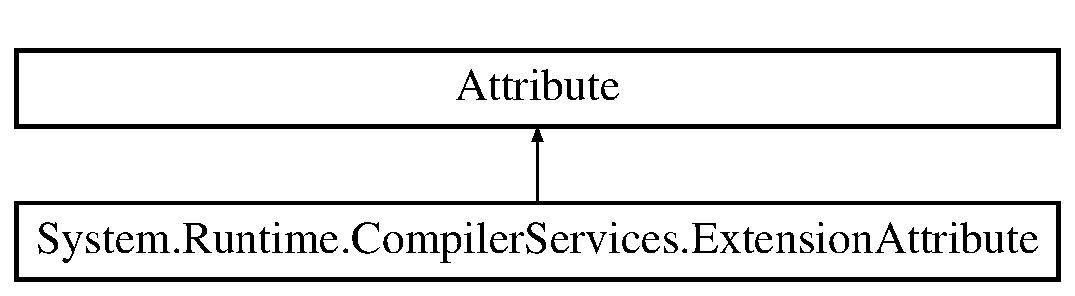
\includegraphics[height=2.000000cm]{class_system_1_1_runtime_1_1_compiler_services_1_1_extension_attribute}
\end{center}
\end{figure}


\subsection{详细描述}


在文件 Tree\-Item.\-cs 第 18 行定义.



该类的文档由以下文件生成\-:\begin{DoxyCompactItemize}
\item 
D\-:/\-My\-Data/\-My\-Git/\-Git\-Hub/\-X\-C\-L\-Net\-Tools/\-X\-C\-L\-Net\-Tools/\-Entity/\-Easy\-U\-I/\hyperlink{_tree_item_8cs}{Tree\-Item.\-cs}\end{DoxyCompactItemize}

\hypertarget{class_x_c_l_net_tools_1_1_file_handler_1_1_file_directory}{}\section{X\+C\+L\+Net\+Tools.\+File\+Handler.\+File\+Directory类 参考}
\label{class_x_c_l_net_tools_1_1_file_handler_1_1_file_directory}\index{X\+C\+L\+Net\+Tools.\+File\+Handler.\+File\+Directory@{X\+C\+L\+Net\+Tools.\+File\+Handler.\+File\+Directory}}


文件目录操作类  


\subsection*{静态 Public 成员函数}
\begin{DoxyCompactItemize}
\item 
static bool \hyperlink{class_x_c_l_net_tools_1_1_file_handler_1_1_file_directory_ac644b5cfdbc06559b2691ca6751506df}{Is\+Empty} (string path)
\begin{DoxyCompactList}\small\item\em 检测目录是否为空目录(既没有文件夹,也没有文件) \end{DoxyCompactList}\item 
static bool \hyperlink{class_x_c_l_net_tools_1_1_file_handler_1_1_file_directory_a1bc5d74fb797d8f8271caf1601f428fe}{Directory\+Exists} (string directory\+Name)
\begin{DoxyCompactList}\small\item\em 判断目录是否存在 \end{DoxyCompactList}\item 
static bool \hyperlink{class_x_c_l_net_tools_1_1_file_handler_1_1_file_directory_a8f3ce048a9225a0b699d7bbc510bd9e3}{Make\+Directory} (string directory\+Name)
\begin{DoxyCompactList}\small\item\em 建立目录 \end{DoxyCompactList}\item 
static bool \hyperlink{class_x_c_l_net_tools_1_1_file_handler_1_1_file_directory_aea79f469e66f1668c6bb4eff61bf9279}{R\+M\+D\+IR} (string directory\+Name)
\begin{DoxyCompactList}\small\item\em 删除指定的目录 \end{DoxyCompactList}\item 
static bool \hyperlink{class_x_c_l_net_tools_1_1_file_handler_1_1_file_directory_a1810da560c803121e71fa92fd4f9d180}{Del\+Tree} (string directory\+Name)
\begin{DoxyCompactList}\small\item\em 删除目录并删除其下的子目录及其文件 \end{DoxyCompactList}\item 
static bool \hyperlink{class_x_c_l_net_tools_1_1_file_handler_1_1_file_directory_a1f64c69d3e2dc580b54a93fe0c871178}{Clear\+Directory} (string root\+Path)
\begin{DoxyCompactList}\small\item\em 清空指定目录 \end{DoxyCompactList}\item 
static List$<$ \hyperlink{class_x_c_l_net_tools_1_1_entity_1_1_file_info_entity}{X\+C\+L\+Net\+Tools.\+Entity.\+File\+Info\+Entity} $>$ \hyperlink{class_x_c_l_net_tools_1_1_file_handler_1_1_file_directory_ac145cab935d17a93ec683d1763bfdccd}{Get\+File\+List} (string dir\+Path, string root\+Path=\char`\"{}\char`\"{}, string web\+Root\+Path=\char`\"{}\char`\"{})
\begin{DoxyCompactList}\small\item\em 获取指定目录下的所有文件及文件夹信息 \end{DoxyCompactList}\item 
static bool \hyperlink{class_x_c_l_net_tools_1_1_file_handler_1_1_file_directory_a40110c2de9ef47ac099acdbbf0703a0c}{Create\+Text\+File} (string file\+Path\+Name)
\begin{DoxyCompactList}\small\item\em 建立一个文件 \end{DoxyCompactList}\item 
static void \hyperlink{class_x_c_l_net_tools_1_1_file_handler_1_1_file_directory_a7153ad7012f2c7259a89cc1f44fa57e2}{Append\+Text} (string file\+Path\+Name, string write\+Word)
\begin{DoxyCompactList}\small\item\em 在文件里追加内容 \end{DoxyCompactList}\item 
static void \hyperlink{class_x_c_l_net_tools_1_1_file_handler_1_1_file_directory_a15ae657816572db98e886f45b2949f76}{Append\+Text} (string file\+Path\+Name, string write\+Word, System.\+Text.\+Encoding encode)
\begin{DoxyCompactList}\small\item\em 在文件里追加内容 \end{DoxyCompactList}\item 
static string \hyperlink{class_x_c_l_net_tools_1_1_file_handler_1_1_file_directory_a5658b6c4ee9c9d4035033e5eb5ac773b}{Read\+File\+Data} (string file\+Path\+Name)
\begin{DoxyCompactList}\small\item\em 读取文件里内容 \end{DoxyCompactList}\item 
static bool \hyperlink{class_x_c_l_net_tools_1_1_file_handler_1_1_file_directory_a8ce6f5c7bf94c4fe2770993cef7be536}{File\+Delete} (string absolute\+File\+Path)
\begin{DoxyCompactList}\small\item\em 删除文件 \end{DoxyCompactList}\end{DoxyCompactItemize}


\subsection{详细描述}
文件目录操作类 



在文件 File\+Directory.\+cs 第 18 行定义.



\subsection{成员函数说明}
\mbox{\Hypertarget{class_x_c_l_net_tools_1_1_file_handler_1_1_file_directory_a7153ad7012f2c7259a89cc1f44fa57e2}\label{class_x_c_l_net_tools_1_1_file_handler_1_1_file_directory_a7153ad7012f2c7259a89cc1f44fa57e2}} 
\index{X\+C\+L\+Net\+Tools\+::\+File\+Handler\+::\+File\+Directory@{X\+C\+L\+Net\+Tools\+::\+File\+Handler\+::\+File\+Directory}!Append\+Text@{Append\+Text}}
\index{Append\+Text@{Append\+Text}!X\+C\+L\+Net\+Tools\+::\+File\+Handler\+::\+File\+Directory@{X\+C\+L\+Net\+Tools\+::\+File\+Handler\+::\+File\+Directory}}
\subsubsection{\texorpdfstring{Append\+Text()}{AppendText()}\hspace{0.1cm}{\footnotesize\ttfamily [1/2]}}
{\footnotesize\ttfamily static void X\+C\+L\+Net\+Tools.\+File\+Handler.\+File\+Directory.\+Append\+Text (\begin{DoxyParamCaption}\item[{string}]{file\+Path\+Name,  }\item[{string}]{write\+Word }\end{DoxyParamCaption})\hspace{0.3cm}{\ttfamily [static]}}



在文件里追加内容 


\begin{DoxyParams}{参数}
{\em file\+Path\+Name} & 文件名\\
\hline
{\em write\+Word} & 追加内容\\
\hline
\end{DoxyParams}


在文件 File\+Directory.\+cs 第 245 行定义.

\mbox{\Hypertarget{class_x_c_l_net_tools_1_1_file_handler_1_1_file_directory_a15ae657816572db98e886f45b2949f76}\label{class_x_c_l_net_tools_1_1_file_handler_1_1_file_directory_a15ae657816572db98e886f45b2949f76}} 
\index{X\+C\+L\+Net\+Tools\+::\+File\+Handler\+::\+File\+Directory@{X\+C\+L\+Net\+Tools\+::\+File\+Handler\+::\+File\+Directory}!Append\+Text@{Append\+Text}}
\index{Append\+Text@{Append\+Text}!X\+C\+L\+Net\+Tools\+::\+File\+Handler\+::\+File\+Directory@{X\+C\+L\+Net\+Tools\+::\+File\+Handler\+::\+File\+Directory}}
\subsubsection{\texorpdfstring{Append\+Text()}{AppendText()}\hspace{0.1cm}{\footnotesize\ttfamily [2/2]}}
{\footnotesize\ttfamily static void X\+C\+L\+Net\+Tools.\+File\+Handler.\+File\+Directory.\+Append\+Text (\begin{DoxyParamCaption}\item[{string}]{file\+Path\+Name,  }\item[{string}]{write\+Word,  }\item[{System.\+Text.\+Encoding}]{encode }\end{DoxyParamCaption})\hspace{0.3cm}{\ttfamily [static]}}



在文件里追加内容 


\begin{DoxyParams}{参数}
{\em file\+Path\+Name} & 文件名\\
\hline
{\em write\+Word} & 追加内容\\
\hline
{\em encode} & 编码\\
\hline
\end{DoxyParams}


在文件 File\+Directory.\+cs 第 256 行定义.

\mbox{\Hypertarget{class_x_c_l_net_tools_1_1_file_handler_1_1_file_directory_a1f64c69d3e2dc580b54a93fe0c871178}\label{class_x_c_l_net_tools_1_1_file_handler_1_1_file_directory_a1f64c69d3e2dc580b54a93fe0c871178}} 
\index{X\+C\+L\+Net\+Tools\+::\+File\+Handler\+::\+File\+Directory@{X\+C\+L\+Net\+Tools\+::\+File\+Handler\+::\+File\+Directory}!Clear\+Directory@{Clear\+Directory}}
\index{Clear\+Directory@{Clear\+Directory}!X\+C\+L\+Net\+Tools\+::\+File\+Handler\+::\+File\+Directory@{X\+C\+L\+Net\+Tools\+::\+File\+Handler\+::\+File\+Directory}}
\subsubsection{\texorpdfstring{Clear\+Directory()}{ClearDirectory()}}
{\footnotesize\ttfamily static bool X\+C\+L\+Net\+Tools.\+File\+Handler.\+File\+Directory.\+Clear\+Directory (\begin{DoxyParamCaption}\item[{string}]{root\+Path }\end{DoxyParamCaption})\hspace{0.3cm}{\ttfamily [static]}}



清空指定目录 


\begin{DoxyParams}{参数}
{\em root\+Path} & 要清空的目录\\
\hline
\end{DoxyParams}
\begin{DoxyReturn}{返回}
是否操作成功
\end{DoxyReturn}


在文件 File\+Directory.\+cs 第 115 行定义.

\mbox{\Hypertarget{class_x_c_l_net_tools_1_1_file_handler_1_1_file_directory_a40110c2de9ef47ac099acdbbf0703a0c}\label{class_x_c_l_net_tools_1_1_file_handler_1_1_file_directory_a40110c2de9ef47ac099acdbbf0703a0c}} 
\index{X\+C\+L\+Net\+Tools\+::\+File\+Handler\+::\+File\+Directory@{X\+C\+L\+Net\+Tools\+::\+File\+Handler\+::\+File\+Directory}!Create\+Text\+File@{Create\+Text\+File}}
\index{Create\+Text\+File@{Create\+Text\+File}!X\+C\+L\+Net\+Tools\+::\+File\+Handler\+::\+File\+Directory@{X\+C\+L\+Net\+Tools\+::\+File\+Handler\+::\+File\+Directory}}
\subsubsection{\texorpdfstring{Create\+Text\+File()}{CreateTextFile()}}
{\footnotesize\ttfamily static bool X\+C\+L\+Net\+Tools.\+File\+Handler.\+File\+Directory.\+Create\+Text\+File (\begin{DoxyParamCaption}\item[{string}]{file\+Path\+Name }\end{DoxyParamCaption})\hspace{0.3cm}{\ttfamily [static]}}



建立一个文件 


\begin{DoxyParams}{参数}
{\em file\+Path\+Name} & 目录名\\
\hline
\end{DoxyParams}
\begin{DoxyReturn}{返回}
true\+:建立成功,false\+:建立失败
\end{DoxyReturn}


在文件 File\+Directory.\+cs 第 223 行定义.

\mbox{\Hypertarget{class_x_c_l_net_tools_1_1_file_handler_1_1_file_directory_a1810da560c803121e71fa92fd4f9d180}\label{class_x_c_l_net_tools_1_1_file_handler_1_1_file_directory_a1810da560c803121e71fa92fd4f9d180}} 
\index{X\+C\+L\+Net\+Tools\+::\+File\+Handler\+::\+File\+Directory@{X\+C\+L\+Net\+Tools\+::\+File\+Handler\+::\+File\+Directory}!Del\+Tree@{Del\+Tree}}
\index{Del\+Tree@{Del\+Tree}!X\+C\+L\+Net\+Tools\+::\+File\+Handler\+::\+File\+Directory@{X\+C\+L\+Net\+Tools\+::\+File\+Handler\+::\+File\+Directory}}
\subsubsection{\texorpdfstring{Del\+Tree()}{DelTree()}}
{\footnotesize\ttfamily static bool X\+C\+L\+Net\+Tools.\+File\+Handler.\+File\+Directory.\+Del\+Tree (\begin{DoxyParamCaption}\item[{string}]{directory\+Name }\end{DoxyParamCaption})\hspace{0.3cm}{\ttfamily [static]}}



删除目录并删除其下的子目录及其文件 


\begin{DoxyParams}{参数}
{\em directory\+Name} & 目录名\\
\hline
\end{DoxyParams}
\begin{DoxyReturn}{返回}
true\+:删除成功,false\+:删除失败
\end{DoxyReturn}


在文件 File\+Directory.\+cs 第 97 行定义.

\mbox{\Hypertarget{class_x_c_l_net_tools_1_1_file_handler_1_1_file_directory_a1bc5d74fb797d8f8271caf1601f428fe}\label{class_x_c_l_net_tools_1_1_file_handler_1_1_file_directory_a1bc5d74fb797d8f8271caf1601f428fe}} 
\index{X\+C\+L\+Net\+Tools\+::\+File\+Handler\+::\+File\+Directory@{X\+C\+L\+Net\+Tools\+::\+File\+Handler\+::\+File\+Directory}!Directory\+Exists@{Directory\+Exists}}
\index{Directory\+Exists@{Directory\+Exists}!X\+C\+L\+Net\+Tools\+::\+File\+Handler\+::\+File\+Directory@{X\+C\+L\+Net\+Tools\+::\+File\+Handler\+::\+File\+Directory}}
\subsubsection{\texorpdfstring{Directory\+Exists()}{DirectoryExists()}}
{\footnotesize\ttfamily static bool X\+C\+L\+Net\+Tools.\+File\+Handler.\+File\+Directory.\+Directory\+Exists (\begin{DoxyParamCaption}\item[{string}]{directory\+Name }\end{DoxyParamCaption})\hspace{0.3cm}{\ttfamily [static]}}



判断目录是否存在 


\begin{DoxyParams}{参数}
{\em directory\+Name} & 目录路径\\
\hline
\end{DoxyParams}
\begin{DoxyReturn}{返回}
true:存在,false:不存在
\end{DoxyReturn}


在文件 File\+Directory.\+cs 第 43 行定义.

\mbox{\Hypertarget{class_x_c_l_net_tools_1_1_file_handler_1_1_file_directory_a8ce6f5c7bf94c4fe2770993cef7be536}\label{class_x_c_l_net_tools_1_1_file_handler_1_1_file_directory_a8ce6f5c7bf94c4fe2770993cef7be536}} 
\index{X\+C\+L\+Net\+Tools\+::\+File\+Handler\+::\+File\+Directory@{X\+C\+L\+Net\+Tools\+::\+File\+Handler\+::\+File\+Directory}!File\+Delete@{File\+Delete}}
\index{File\+Delete@{File\+Delete}!X\+C\+L\+Net\+Tools\+::\+File\+Handler\+::\+File\+Directory@{X\+C\+L\+Net\+Tools\+::\+File\+Handler\+::\+File\+Directory}}
\subsubsection{\texorpdfstring{File\+Delete()}{FileDelete()}}
{\footnotesize\ttfamily static bool X\+C\+L\+Net\+Tools.\+File\+Handler.\+File\+Directory.\+File\+Delete (\begin{DoxyParamCaption}\item[{string}]{absolute\+File\+Path }\end{DoxyParamCaption})\hspace{0.3cm}{\ttfamily [static]}}



删除文件 


\begin{DoxyParams}{参数}
{\em absolute\+File\+Path} & 文件绝对地址\\
\hline
\end{DoxyParams}
\begin{DoxyReturn}{返回}
true\+:删除文件成功,false\+:删除文件失败
\end{DoxyReturn}


在文件 File\+Directory.\+cs 第 292 行定义.

\mbox{\Hypertarget{class_x_c_l_net_tools_1_1_file_handler_1_1_file_directory_ac145cab935d17a93ec683d1763bfdccd}\label{class_x_c_l_net_tools_1_1_file_handler_1_1_file_directory_ac145cab935d17a93ec683d1763bfdccd}} 
\index{X\+C\+L\+Net\+Tools\+::\+File\+Handler\+::\+File\+Directory@{X\+C\+L\+Net\+Tools\+::\+File\+Handler\+::\+File\+Directory}!Get\+File\+List@{Get\+File\+List}}
\index{Get\+File\+List@{Get\+File\+List}!X\+C\+L\+Net\+Tools\+::\+File\+Handler\+::\+File\+Directory@{X\+C\+L\+Net\+Tools\+::\+File\+Handler\+::\+File\+Directory}}
\subsubsection{\texorpdfstring{Get\+File\+List()}{GetFileList()}}
{\footnotesize\ttfamily static List$<$\hyperlink{class_x_c_l_net_tools_1_1_entity_1_1_file_info_entity}{X\+C\+L\+Net\+Tools.\+Entity.\+File\+Info\+Entity}$>$ X\+C\+L\+Net\+Tools.\+File\+Handler.\+File\+Directory.\+Get\+File\+List (\begin{DoxyParamCaption}\item[{string}]{dir\+Path,  }\item[{string}]{root\+Path = {\ttfamily \char`\"{}\char`\"{}},  }\item[{string}]{web\+Root\+Path = {\ttfamily \char`\"{}\char`\"{}} }\end{DoxyParamCaption})\hspace{0.3cm}{\ttfamily [static]}}



获取指定目录下的所有文件及文件夹信息 


\begin{DoxyParams}{参数}
{\em dir\+Path} & 要获取信息的目录路径\\
\hline
{\em root\+Path} & 根路径(设置该值后,返回的信息实体中将包含相对于该根路径的相对路径信息)\\
\hline
{\em web\+Root\+Path} & web根路径(用于生成该文件或文件夹的web路径),如:http\+://www.a.\+com/web/\\
\hline
\end{DoxyParams}
\begin{DoxyReturn}{返回}
文件信息list
\end{DoxyReturn}


在文件 File\+Directory.\+cs 第 142 行定义.

\mbox{\Hypertarget{class_x_c_l_net_tools_1_1_file_handler_1_1_file_directory_ac644b5cfdbc06559b2691ca6751506df}\label{class_x_c_l_net_tools_1_1_file_handler_1_1_file_directory_ac644b5cfdbc06559b2691ca6751506df}} 
\index{X\+C\+L\+Net\+Tools\+::\+File\+Handler\+::\+File\+Directory@{X\+C\+L\+Net\+Tools\+::\+File\+Handler\+::\+File\+Directory}!Is\+Empty@{Is\+Empty}}
\index{Is\+Empty@{Is\+Empty}!X\+C\+L\+Net\+Tools\+::\+File\+Handler\+::\+File\+Directory@{X\+C\+L\+Net\+Tools\+::\+File\+Handler\+::\+File\+Directory}}
\subsubsection{\texorpdfstring{Is\+Empty()}{IsEmpty()}}
{\footnotesize\ttfamily static bool X\+C\+L\+Net\+Tools.\+File\+Handler.\+File\+Directory.\+Is\+Empty (\begin{DoxyParamCaption}\item[{string}]{path }\end{DoxyParamCaption})\hspace{0.3cm}{\ttfamily [static]}}



检测目录是否为空目录(既没有文件夹,也没有文件) 


\begin{DoxyParams}{参数}
{\em path} & 目录路径\\
\hline
\end{DoxyParams}
\begin{DoxyReturn}{返回}
true\+:空目录,false\+:非空目录
\end{DoxyReturn}


在文件 File\+Directory.\+cs 第 27 行定义.

\mbox{\Hypertarget{class_x_c_l_net_tools_1_1_file_handler_1_1_file_directory_a8f3ce048a9225a0b699d7bbc510bd9e3}\label{class_x_c_l_net_tools_1_1_file_handler_1_1_file_directory_a8f3ce048a9225a0b699d7bbc510bd9e3}} 
\index{X\+C\+L\+Net\+Tools\+::\+File\+Handler\+::\+File\+Directory@{X\+C\+L\+Net\+Tools\+::\+File\+Handler\+::\+File\+Directory}!Make\+Directory@{Make\+Directory}}
\index{Make\+Directory@{Make\+Directory}!X\+C\+L\+Net\+Tools\+::\+File\+Handler\+::\+File\+Directory@{X\+C\+L\+Net\+Tools\+::\+File\+Handler\+::\+File\+Directory}}
\subsubsection{\texorpdfstring{Make\+Directory()}{MakeDirectory()}}
{\footnotesize\ttfamily static bool X\+C\+L\+Net\+Tools.\+File\+Handler.\+File\+Directory.\+Make\+Directory (\begin{DoxyParamCaption}\item[{string}]{directory\+Name }\end{DoxyParamCaption})\hspace{0.3cm}{\ttfamily [static]}}



建立目录 


\begin{DoxyParams}{参数}
{\em directory\+Name} & 目录名\\
\hline
\end{DoxyParams}
\begin{DoxyReturn}{返回}
返回boolean,true\+:目录建立成功, false\+:目录建立失败
\end{DoxyReturn}


在文件 File\+Directory.\+cs 第 53 行定义.

\mbox{\Hypertarget{class_x_c_l_net_tools_1_1_file_handler_1_1_file_directory_a5658b6c4ee9c9d4035033e5eb5ac773b}\label{class_x_c_l_net_tools_1_1_file_handler_1_1_file_directory_a5658b6c4ee9c9d4035033e5eb5ac773b}} 
\index{X\+C\+L\+Net\+Tools\+::\+File\+Handler\+::\+File\+Directory@{X\+C\+L\+Net\+Tools\+::\+File\+Handler\+::\+File\+Directory}!Read\+File\+Data@{Read\+File\+Data}}
\index{Read\+File\+Data@{Read\+File\+Data}!X\+C\+L\+Net\+Tools\+::\+File\+Handler\+::\+File\+Directory@{X\+C\+L\+Net\+Tools\+::\+File\+Handler\+::\+File\+Directory}}
\subsubsection{\texorpdfstring{Read\+File\+Data()}{ReadFileData()}}
{\footnotesize\ttfamily static string X\+C\+L\+Net\+Tools.\+File\+Handler.\+File\+Directory.\+Read\+File\+Data (\begin{DoxyParamCaption}\item[{string}]{file\+Path\+Name }\end{DoxyParamCaption})\hspace{0.3cm}{\ttfamily [static]}}



读取文件里内容 


\begin{DoxyParams}{参数}
{\em file\+Path\+Name} & 文件名\\
\hline
\end{DoxyParams}
\begin{DoxyReturn}{返回}
文件内容
\end{DoxyReturn}


在文件 File\+Directory.\+cs 第 276 行定义.

\mbox{\Hypertarget{class_x_c_l_net_tools_1_1_file_handler_1_1_file_directory_aea79f469e66f1668c6bb4eff61bf9279}\label{class_x_c_l_net_tools_1_1_file_handler_1_1_file_directory_aea79f469e66f1668c6bb4eff61bf9279}} 
\index{X\+C\+L\+Net\+Tools\+::\+File\+Handler\+::\+File\+Directory@{X\+C\+L\+Net\+Tools\+::\+File\+Handler\+::\+File\+Directory}!R\+M\+D\+IR@{R\+M\+D\+IR}}
\index{R\+M\+D\+IR@{R\+M\+D\+IR}!X\+C\+L\+Net\+Tools\+::\+File\+Handler\+::\+File\+Directory@{X\+C\+L\+Net\+Tools\+::\+File\+Handler\+::\+File\+Directory}}
\subsubsection{\texorpdfstring{R\+M\+D\+I\+R()}{RMDIR()}}
{\footnotesize\ttfamily static bool X\+C\+L\+Net\+Tools.\+File\+Handler.\+File\+Directory.\+R\+M\+D\+IR (\begin{DoxyParamCaption}\item[{string}]{directory\+Name }\end{DoxyParamCaption})\hspace{0.3cm}{\ttfamily [static]}}



删除指定的目录 


\begin{DoxyParams}{参数}
{\em directory\+Name} & 目录名\\
\hline
\end{DoxyParams}
\begin{DoxyReturn}{返回}
true:删除成功,false:删除失败
\end{DoxyReturn}


在文件 File\+Directory.\+cs 第 78 行定义.



该类的文档由以下文件生成\+:\begin{DoxyCompactItemize}
\item 
D\+:/\+My\+Data/\+Git\+Hub/\+X\+C\+L\+Net\+Tools/\+X\+C\+L\+Net\+Tools/\+File\+Handler/\hyperlink{_file_directory_8cs}{File\+Directory.\+cs}\end{DoxyCompactItemize}

\hypertarget{class_x_c_l_net_tools_1_1_entity_1_1_file_info_entity}{\section{X\-C\-L\-Net\-Tools.\-Entity.\-File\-Info\-Entity类 参考}
\label{class_x_c_l_net_tools_1_1_entity_1_1_file_info_entity}\index{X\-C\-L\-Net\-Tools.\-Entity.\-File\-Info\-Entity@{X\-C\-L\-Net\-Tools.\-Entity.\-File\-Info\-Entity}}
}


文件信息实体  


\subsection*{属性}
\begin{DoxyCompactItemize}
\item 
int \hyperlink{class_x_c_l_net_tools_1_1_entity_1_1_file_info_entity_a150f26081f12badeea9a2255bbea6faf}{I\-D}\hspace{0.3cm}{\ttfamily  \mbox{[}get, set\mbox{]}}
\begin{DoxyCompactList}\small\item\em 标识\-I\-D \end{DoxyCompactList}\item 
bool \hyperlink{class_x_c_l_net_tools_1_1_entity_1_1_file_info_entity_ad945716535742c01f83dffc2766c0987}{Is\-Folder}\hspace{0.3cm}{\ttfamily  \mbox{[}get, set\mbox{]}}
\begin{DoxyCompactList}\small\item\em 是否为文件夹 \end{DoxyCompactList}\item 
string \hyperlink{class_x_c_l_net_tools_1_1_entity_1_1_file_info_entity_a15a2bb6c738c32250f00604b6636cae4}{Name}\hspace{0.3cm}{\ttfamily  \mbox{[}get, set\mbox{]}}
\begin{DoxyCompactList}\small\item\em 文件名 \end{DoxyCompactList}\item 
string \hyperlink{class_x_c_l_net_tools_1_1_entity_1_1_file_info_entity_a46ccaf5dbcc1154782c0227c83eb54e4}{Ext\-Name}\hspace{0.3cm}{\ttfamily  \mbox{[}get, set\mbox{]}}
\begin{DoxyCompactList}\small\item\em 扩展名(不含小圆点) \end{DoxyCompactList}\item 
string \hyperlink{class_x_c_l_net_tools_1_1_entity_1_1_file_info_entity_a6ef4c659747c605379a43168ae1d64f6}{Root\-Path}\hspace{0.3cm}{\ttfamily  \mbox{[}get, set\mbox{]}}
\begin{DoxyCompactList}\small\item\em 根物理路径 \end{DoxyCompactList}\item 
string \hyperlink{class_x_c_l_net_tools_1_1_entity_1_1_file_info_entity_a67f485c1a1af6205351305756d515e98}{Path}\hspace{0.3cm}{\ttfamily  \mbox{[}get, set\mbox{]}}
\begin{DoxyCompactList}\small\item\em 该文件或文件夹的物理路径 \end{DoxyCompactList}\item 
string \hyperlink{class_x_c_l_net_tools_1_1_entity_1_1_file_info_entity_ab93bd802770bb40cc0abdfd35d2fbbc6}{Web\-Path}\hspace{0.3cm}{\ttfamily  \mbox{[}get, set\mbox{]}}
\begin{DoxyCompactList}\small\item\em 该文件或文件夹的web路径 \end{DoxyCompactList}\item 
string \hyperlink{class_x_c_l_net_tools_1_1_entity_1_1_file_info_entity_a795982d186fa2d1ef0e3fb51705f36b2}{Relative\-Path}\hspace{0.3cm}{\ttfamily  \mbox{[}get, set\mbox{]}}
\begin{DoxyCompactList}\small\item\em 该文件或文件夹相对于\-Root\-Path的相对路径 \end{DoxyCompactList}\item 
long \hyperlink{class_x_c_l_net_tools_1_1_entity_1_1_file_info_entity_a7447a43994e75793388e160a626ba346}{Size}\hspace{0.3cm}{\ttfamily  \mbox{[}get, set\mbox{]}}
\begin{DoxyCompactList}\small\item\em 大小(byte) \end{DoxyCompactList}\item 
Date\-Time \hyperlink{class_x_c_l_net_tools_1_1_entity_1_1_file_info_entity_a64c6633bec7e4d547632c122dbaad9f8}{Modify\-Time}\hspace{0.3cm}{\ttfamily  \mbox{[}get, set\mbox{]}}
\begin{DoxyCompactList}\small\item\em 修改时间 \end{DoxyCompactList}\item 
Date\-Time \hyperlink{class_x_c_l_net_tools_1_1_entity_1_1_file_info_entity_a93fc7b2a3119885d9449d1817e7306ca}{Create\-Time}\hspace{0.3cm}{\ttfamily  \mbox{[}get, set\mbox{]}}
\begin{DoxyCompactList}\small\item\em 创建时间 \end{DoxyCompactList}\end{DoxyCompactItemize}


\subsection{详细描述}
文件信息实体 



在文件 File\-Info\-Entity.\-cs 第 17 行定义.



\subsection{属性说明}
\hypertarget{class_x_c_l_net_tools_1_1_entity_1_1_file_info_entity_a93fc7b2a3119885d9449d1817e7306ca}{\index{X\-C\-L\-Net\-Tools\-::\-Entity\-::\-File\-Info\-Entity@{X\-C\-L\-Net\-Tools\-::\-Entity\-::\-File\-Info\-Entity}!Create\-Time@{Create\-Time}}
\index{Create\-Time@{Create\-Time}!XCLNetTools::Entity::FileInfoEntity@{X\-C\-L\-Net\-Tools\-::\-Entity\-::\-File\-Info\-Entity}}
\subsubsection[{Create\-Time}]{\setlength{\rightskip}{0pt plus 5cm}Date\-Time X\-C\-L\-Net\-Tools.\-Entity.\-File\-Info\-Entity.\-Create\-Time\hspace{0.3cm}{\ttfamily [get]}, {\ttfamily [set]}}}\label{class_x_c_l_net_tools_1_1_entity_1_1_file_info_entity_a93fc7b2a3119885d9449d1817e7306ca}


创建时间 



在文件 File\-Info\-Entity.\-cs 第 72 行定义.

\hypertarget{class_x_c_l_net_tools_1_1_entity_1_1_file_info_entity_a46ccaf5dbcc1154782c0227c83eb54e4}{\index{X\-C\-L\-Net\-Tools\-::\-Entity\-::\-File\-Info\-Entity@{X\-C\-L\-Net\-Tools\-::\-Entity\-::\-File\-Info\-Entity}!Ext\-Name@{Ext\-Name}}
\index{Ext\-Name@{Ext\-Name}!XCLNetTools::Entity::FileInfoEntity@{X\-C\-L\-Net\-Tools\-::\-Entity\-::\-File\-Info\-Entity}}
\subsubsection[{Ext\-Name}]{\setlength{\rightskip}{0pt plus 5cm}string X\-C\-L\-Net\-Tools.\-Entity.\-File\-Info\-Entity.\-Ext\-Name\hspace{0.3cm}{\ttfamily [get]}, {\ttfamily [set]}}}\label{class_x_c_l_net_tools_1_1_entity_1_1_file_info_entity_a46ccaf5dbcc1154782c0227c83eb54e4}


扩展名(不含小圆点) 



在文件 File\-Info\-Entity.\-cs 第 37 行定义.

\hypertarget{class_x_c_l_net_tools_1_1_entity_1_1_file_info_entity_a150f26081f12badeea9a2255bbea6faf}{\index{X\-C\-L\-Net\-Tools\-::\-Entity\-::\-File\-Info\-Entity@{X\-C\-L\-Net\-Tools\-::\-Entity\-::\-File\-Info\-Entity}!I\-D@{I\-D}}
\index{I\-D@{I\-D}!XCLNetTools::Entity::FileInfoEntity@{X\-C\-L\-Net\-Tools\-::\-Entity\-::\-File\-Info\-Entity}}
\subsubsection[{I\-D}]{\setlength{\rightskip}{0pt plus 5cm}int X\-C\-L\-Net\-Tools.\-Entity.\-File\-Info\-Entity.\-I\-D\hspace{0.3cm}{\ttfamily [get]}, {\ttfamily [set]}}}\label{class_x_c_l_net_tools_1_1_entity_1_1_file_info_entity_a150f26081f12badeea9a2255bbea6faf}


标识\-I\-D 



在文件 File\-Info\-Entity.\-cs 第 22 行定义.

\hypertarget{class_x_c_l_net_tools_1_1_entity_1_1_file_info_entity_ad945716535742c01f83dffc2766c0987}{\index{X\-C\-L\-Net\-Tools\-::\-Entity\-::\-File\-Info\-Entity@{X\-C\-L\-Net\-Tools\-::\-Entity\-::\-File\-Info\-Entity}!Is\-Folder@{Is\-Folder}}
\index{Is\-Folder@{Is\-Folder}!XCLNetTools::Entity::FileInfoEntity@{X\-C\-L\-Net\-Tools\-::\-Entity\-::\-File\-Info\-Entity}}
\subsubsection[{Is\-Folder}]{\setlength{\rightskip}{0pt plus 5cm}bool X\-C\-L\-Net\-Tools.\-Entity.\-File\-Info\-Entity.\-Is\-Folder\hspace{0.3cm}{\ttfamily [get]}, {\ttfamily [set]}}}\label{class_x_c_l_net_tools_1_1_entity_1_1_file_info_entity_ad945716535742c01f83dffc2766c0987}


是否为文件夹 



在文件 File\-Info\-Entity.\-cs 第 27 行定义.

\hypertarget{class_x_c_l_net_tools_1_1_entity_1_1_file_info_entity_a64c6633bec7e4d547632c122dbaad9f8}{\index{X\-C\-L\-Net\-Tools\-::\-Entity\-::\-File\-Info\-Entity@{X\-C\-L\-Net\-Tools\-::\-Entity\-::\-File\-Info\-Entity}!Modify\-Time@{Modify\-Time}}
\index{Modify\-Time@{Modify\-Time}!XCLNetTools::Entity::FileInfoEntity@{X\-C\-L\-Net\-Tools\-::\-Entity\-::\-File\-Info\-Entity}}
\subsubsection[{Modify\-Time}]{\setlength{\rightskip}{0pt plus 5cm}Date\-Time X\-C\-L\-Net\-Tools.\-Entity.\-File\-Info\-Entity.\-Modify\-Time\hspace{0.3cm}{\ttfamily [get]}, {\ttfamily [set]}}}\label{class_x_c_l_net_tools_1_1_entity_1_1_file_info_entity_a64c6633bec7e4d547632c122dbaad9f8}


修改时间 



在文件 File\-Info\-Entity.\-cs 第 67 行定义.

\hypertarget{class_x_c_l_net_tools_1_1_entity_1_1_file_info_entity_a15a2bb6c738c32250f00604b6636cae4}{\index{X\-C\-L\-Net\-Tools\-::\-Entity\-::\-File\-Info\-Entity@{X\-C\-L\-Net\-Tools\-::\-Entity\-::\-File\-Info\-Entity}!Name@{Name}}
\index{Name@{Name}!XCLNetTools::Entity::FileInfoEntity@{X\-C\-L\-Net\-Tools\-::\-Entity\-::\-File\-Info\-Entity}}
\subsubsection[{Name}]{\setlength{\rightskip}{0pt plus 5cm}string X\-C\-L\-Net\-Tools.\-Entity.\-File\-Info\-Entity.\-Name\hspace{0.3cm}{\ttfamily [get]}, {\ttfamily [set]}}}\label{class_x_c_l_net_tools_1_1_entity_1_1_file_info_entity_a15a2bb6c738c32250f00604b6636cae4}


文件名 



在文件 File\-Info\-Entity.\-cs 第 32 行定义.

\hypertarget{class_x_c_l_net_tools_1_1_entity_1_1_file_info_entity_a67f485c1a1af6205351305756d515e98}{\index{X\-C\-L\-Net\-Tools\-::\-Entity\-::\-File\-Info\-Entity@{X\-C\-L\-Net\-Tools\-::\-Entity\-::\-File\-Info\-Entity}!Path@{Path}}
\index{Path@{Path}!XCLNetTools::Entity::FileInfoEntity@{X\-C\-L\-Net\-Tools\-::\-Entity\-::\-File\-Info\-Entity}}
\subsubsection[{Path}]{\setlength{\rightskip}{0pt plus 5cm}string X\-C\-L\-Net\-Tools.\-Entity.\-File\-Info\-Entity.\-Path\hspace{0.3cm}{\ttfamily [get]}, {\ttfamily [set]}}}\label{class_x_c_l_net_tools_1_1_entity_1_1_file_info_entity_a67f485c1a1af6205351305756d515e98}


该文件或文件夹的物理路径 



在文件 File\-Info\-Entity.\-cs 第 47 行定义.

\hypertarget{class_x_c_l_net_tools_1_1_entity_1_1_file_info_entity_a795982d186fa2d1ef0e3fb51705f36b2}{\index{X\-C\-L\-Net\-Tools\-::\-Entity\-::\-File\-Info\-Entity@{X\-C\-L\-Net\-Tools\-::\-Entity\-::\-File\-Info\-Entity}!Relative\-Path@{Relative\-Path}}
\index{Relative\-Path@{Relative\-Path}!XCLNetTools::Entity::FileInfoEntity@{X\-C\-L\-Net\-Tools\-::\-Entity\-::\-File\-Info\-Entity}}
\subsubsection[{Relative\-Path}]{\setlength{\rightskip}{0pt plus 5cm}string X\-C\-L\-Net\-Tools.\-Entity.\-File\-Info\-Entity.\-Relative\-Path\hspace{0.3cm}{\ttfamily [get]}, {\ttfamily [set]}}}\label{class_x_c_l_net_tools_1_1_entity_1_1_file_info_entity_a795982d186fa2d1ef0e3fb51705f36b2}


该文件或文件夹相对于\-Root\-Path的相对路径 



在文件 File\-Info\-Entity.\-cs 第 57 行定义.

\hypertarget{class_x_c_l_net_tools_1_1_entity_1_1_file_info_entity_a6ef4c659747c605379a43168ae1d64f6}{\index{X\-C\-L\-Net\-Tools\-::\-Entity\-::\-File\-Info\-Entity@{X\-C\-L\-Net\-Tools\-::\-Entity\-::\-File\-Info\-Entity}!Root\-Path@{Root\-Path}}
\index{Root\-Path@{Root\-Path}!XCLNetTools::Entity::FileInfoEntity@{X\-C\-L\-Net\-Tools\-::\-Entity\-::\-File\-Info\-Entity}}
\subsubsection[{Root\-Path}]{\setlength{\rightskip}{0pt plus 5cm}string X\-C\-L\-Net\-Tools.\-Entity.\-File\-Info\-Entity.\-Root\-Path\hspace{0.3cm}{\ttfamily [get]}, {\ttfamily [set]}}}\label{class_x_c_l_net_tools_1_1_entity_1_1_file_info_entity_a6ef4c659747c605379a43168ae1d64f6}


根物理路径 



在文件 File\-Info\-Entity.\-cs 第 42 行定义.

\hypertarget{class_x_c_l_net_tools_1_1_entity_1_1_file_info_entity_a7447a43994e75793388e160a626ba346}{\index{X\-C\-L\-Net\-Tools\-::\-Entity\-::\-File\-Info\-Entity@{X\-C\-L\-Net\-Tools\-::\-Entity\-::\-File\-Info\-Entity}!Size@{Size}}
\index{Size@{Size}!XCLNetTools::Entity::FileInfoEntity@{X\-C\-L\-Net\-Tools\-::\-Entity\-::\-File\-Info\-Entity}}
\subsubsection[{Size}]{\setlength{\rightskip}{0pt plus 5cm}long X\-C\-L\-Net\-Tools.\-Entity.\-File\-Info\-Entity.\-Size\hspace{0.3cm}{\ttfamily [get]}, {\ttfamily [set]}}}\label{class_x_c_l_net_tools_1_1_entity_1_1_file_info_entity_a7447a43994e75793388e160a626ba346}


大小(byte) 



在文件 File\-Info\-Entity.\-cs 第 62 行定义.

\hypertarget{class_x_c_l_net_tools_1_1_entity_1_1_file_info_entity_ab93bd802770bb40cc0abdfd35d2fbbc6}{\index{X\-C\-L\-Net\-Tools\-::\-Entity\-::\-File\-Info\-Entity@{X\-C\-L\-Net\-Tools\-::\-Entity\-::\-File\-Info\-Entity}!Web\-Path@{Web\-Path}}
\index{Web\-Path@{Web\-Path}!XCLNetTools::Entity::FileInfoEntity@{X\-C\-L\-Net\-Tools\-::\-Entity\-::\-File\-Info\-Entity}}
\subsubsection[{Web\-Path}]{\setlength{\rightskip}{0pt plus 5cm}string X\-C\-L\-Net\-Tools.\-Entity.\-File\-Info\-Entity.\-Web\-Path\hspace{0.3cm}{\ttfamily [get]}, {\ttfamily [set]}}}\label{class_x_c_l_net_tools_1_1_entity_1_1_file_info_entity_ab93bd802770bb40cc0abdfd35d2fbbc6}


该文件或文件夹的web路径 



在文件 File\-Info\-Entity.\-cs 第 52 行定义.



该类的文档由以下文件生成\-:\begin{DoxyCompactItemize}
\item 
D\-:/\-My\-Data/\-My\-Git/\-Git\-Hub/\-X\-C\-L\-Net\-Tools/\-X\-C\-L\-Net\-Tools/\-Entity/\hyperlink{_file_info_entity_8cs}{File\-Info\-Entity.\-cs}\end{DoxyCompactItemize}

\hypertarget{class_x_c_l_net_tools_1_1_string_hander_1_1_form_helper}{}\section{X\+C\+L\+Net\+Tools.\+String\+Hander.\+Form\+Helper类 参考}
\label{class_x_c_l_net_tools_1_1_string_hander_1_1_form_helper}\index{X\+C\+L\+Net\+Tools.\+String\+Hander.\+Form\+Helper@{X\+C\+L\+Net\+Tools.\+String\+Hander.\+Form\+Helper}}


form表单相关  


\subsection*{静态 Public 成员函数}
\begin{DoxyCompactItemize}
\item 
static string \hyperlink{class_x_c_l_net_tools_1_1_string_hander_1_1_form_helper_a8c34c5210ad29ea122ee8320b4f14f9f}{Get\+String} (string name)
\begin{DoxyCompactList}\small\item\em 获取string参数,如果没有此参数,则返回\char`\"{}\char`\"{} \end{DoxyCompactList}\item 
static string \hyperlink{class_x_c_l_net_tools_1_1_string_hander_1_1_form_helper_a953f8f717a6b0b26541f0a06c99fe19c}{Get\+String\+Null} (string name, string default\+Value=null)
\begin{DoxyCompactList}\small\item\em 获取string参数,如果没有此参数,则返回default\+Value(默认为null) \end{DoxyCompactList}\item 
static string\mbox{[}$\,$\mbox{]} \hyperlink{class_x_c_l_net_tools_1_1_string_hander_1_1_form_helper_a9b7680e6e7975889a62f273eaacdf37c}{Get\+String\+Array} (string name)
\begin{DoxyCompactList}\small\item\em 获取数组参数 \end{DoxyCompactList}\item 
static byte \hyperlink{class_x_c_l_net_tools_1_1_string_hander_1_1_form_helper_a9d43824d313342bfc66623f548ad6ad6}{Get\+Byte\+Null} (string name)
\begin{DoxyCompactList}\small\item\em 获取byte?参数 \end{DoxyCompactList}\item 
static byte \hyperlink{class_x_c_l_net_tools_1_1_string_hander_1_1_form_helper_a4b2dafb903bedae1af30683209520136}{Get\+Byte\+Null} (string name, byte?default\+Value)
\begin{DoxyCompactList}\small\item\em 获取byte?参数,默认default\+Value \end{DoxyCompactList}\item 
static byte \hyperlink{class_x_c_l_net_tools_1_1_string_hander_1_1_form_helper_aac299eb0719beba6c618deeed497fd76}{Get\+Byte} (string name)
\begin{DoxyCompactList}\small\item\em 获取byte参数,默认0 \end{DoxyCompactList}\item 
static byte \hyperlink{class_x_c_l_net_tools_1_1_string_hander_1_1_form_helper_aa1090c02b273fe23de21755a7b574a08}{Get\+Byte} (string name, byte default\+Value)
\begin{DoxyCompactList}\small\item\em 获取byte参数,默认default\+Value \end{DoxyCompactList}\item 
static List$<$ byte $>$ \hyperlink{class_x_c_l_net_tools_1_1_string_hander_1_1_form_helper_a575a372579f530e8fa7bce9a7808cf7f}{Get\+Byte\+List} (string name)
\begin{DoxyCompactList}\small\item\em 获取byte参数数组 \end{DoxyCompactList}\item 
static int \hyperlink{class_x_c_l_net_tools_1_1_string_hander_1_1_form_helper_a5f6d473bbc50e60cbd6c5015c1d4b010}{Get\+Int\+Null} (string name)
\begin{DoxyCompactList}\small\item\em 获取int?参数 \end{DoxyCompactList}\item 
static int \hyperlink{class_x_c_l_net_tools_1_1_string_hander_1_1_form_helper_a91af563c9654d78b004215b0d8cc5338}{Get\+Int\+Null} (string name, int?default\+Value)
\begin{DoxyCompactList}\small\item\em 获取int?参数,默认default\+Value \end{DoxyCompactList}\item 
static int \hyperlink{class_x_c_l_net_tools_1_1_string_hander_1_1_form_helper_ad3bcc9178dfa1bdc2d0e459b95d56fb4}{Get\+Int} (string name)
\begin{DoxyCompactList}\small\item\em 获取int参数,默认0 \end{DoxyCompactList}\item 
static int \hyperlink{class_x_c_l_net_tools_1_1_string_hander_1_1_form_helper_ab1cbc4a5f6643c60beaf928081457b6f}{Get\+Int} (string name, int default\+Value)
\begin{DoxyCompactList}\small\item\em 获取int参数,默认default\+Value \end{DoxyCompactList}\item 
static List$<$ int $>$ \hyperlink{class_x_c_l_net_tools_1_1_string_hander_1_1_form_helper_a555eba05a8bdc2cab01e84b91e84f8c5}{Get\+Int\+List} (string name)
\begin{DoxyCompactList}\small\item\em 获取int参数数组 \end{DoxyCompactList}\item 
static short \hyperlink{class_x_c_l_net_tools_1_1_string_hander_1_1_form_helper_afe30b64436d0a1831330cd390f3f4b51}{Get\+Short\+Null} (string name)
\begin{DoxyCompactList}\small\item\em 获取short?参数 \end{DoxyCompactList}\item 
static short \hyperlink{class_x_c_l_net_tools_1_1_string_hander_1_1_form_helper_a23c16178ebaf6132bc6954dd098ed901}{Get\+Short\+Null} (string name, short?default\+Value)
\begin{DoxyCompactList}\small\item\em 获取short?参数,默认default\+Value \end{DoxyCompactList}\item 
static short \hyperlink{class_x_c_l_net_tools_1_1_string_hander_1_1_form_helper_a197c2283e3000030d40e7a50d10471f0}{Get\+Short} (string name)
\begin{DoxyCompactList}\small\item\em 获取short参数,默认0 \end{DoxyCompactList}\item 
static short \hyperlink{class_x_c_l_net_tools_1_1_string_hander_1_1_form_helper_a16b3f8a3141fb74656dc3c857da2099b}{Get\+Short} (string name, short default\+Value)
\begin{DoxyCompactList}\small\item\em 获取short参数,默认default\+Value \end{DoxyCompactList}\item 
static List$<$ short $>$ \hyperlink{class_x_c_l_net_tools_1_1_string_hander_1_1_form_helper_aa99502c5145f156f0e8b714d7ab4c308}{Get\+Short\+List} (string name)
\begin{DoxyCompactList}\small\item\em 获取short参数数组 \end{DoxyCompactList}\item 
static long \hyperlink{class_x_c_l_net_tools_1_1_string_hander_1_1_form_helper_abffef0560d4655c00c5bdd3e4ff087cc}{Get\+Long\+Null} (string name)
\begin{DoxyCompactList}\small\item\em 获取\+Long?参数 \end{DoxyCompactList}\item 
static long \hyperlink{class_x_c_l_net_tools_1_1_string_hander_1_1_form_helper_a7e009fc6b804b15f2015d78ed3581677}{Get\+Long\+Null} (string name, long?default\+Value)
\begin{DoxyCompactList}\small\item\em 获取\+Long?参数,默认default\+Value \end{DoxyCompactList}\item 
static long \hyperlink{class_x_c_l_net_tools_1_1_string_hander_1_1_form_helper_a55353bd867fa827c8eb55a710df02cb1}{Get\+Long} (string name)
\begin{DoxyCompactList}\small\item\em 获取long参数,默认0 \end{DoxyCompactList}\item 
static long \hyperlink{class_x_c_l_net_tools_1_1_string_hander_1_1_form_helper_a51392713a245c7460bb5c823eb664ef8}{Get\+Long} (string name, long default\+Value)
\begin{DoxyCompactList}\small\item\em 获取long参数,默认default\+Value \end{DoxyCompactList}\item 
static List$<$ long $>$ \hyperlink{class_x_c_l_net_tools_1_1_string_hander_1_1_form_helper_ac00bef1db952ab0901c1813bbe193fa0}{Get\+Long\+List} (string name)
\begin{DoxyCompactList}\small\item\em 获取long参数数组 \end{DoxyCompactList}\item 
static float \hyperlink{class_x_c_l_net_tools_1_1_string_hander_1_1_form_helper_a6d0d3c455a9582ca4a4fa5bf4269deff}{Get\+Float\+Null} (string name)
\begin{DoxyCompactList}\small\item\em 获取float?参数 \end{DoxyCompactList}\item 
static float \hyperlink{class_x_c_l_net_tools_1_1_string_hander_1_1_form_helper_a4647a1a2655436ed24cc07f117109818}{Get\+Float\+Null} (string name, float?default\+Value)
\begin{DoxyCompactList}\small\item\em 获取float?参数,默认default\+Value \end{DoxyCompactList}\item 
static float \hyperlink{class_x_c_l_net_tools_1_1_string_hander_1_1_form_helper_a0807fb3fcdf5a5686fe0d8417013835a}{Get\+Float} (string name)
\begin{DoxyCompactList}\small\item\em 获取float参数,默认0 \end{DoxyCompactList}\item 
static float \hyperlink{class_x_c_l_net_tools_1_1_string_hander_1_1_form_helper_acae860acd22e9f85511ccdc60c071c5c}{Get\+Float} (string name, float default\+Value)
\begin{DoxyCompactList}\small\item\em 获取float参数,默认default\+Value \end{DoxyCompactList}\item 
static List$<$ float $>$ \hyperlink{class_x_c_l_net_tools_1_1_string_hander_1_1_form_helper_ad405fffedfe8e34e61e4118754f99fe4}{Get\+Float\+List} (string name)
\begin{DoxyCompactList}\small\item\em 获取float参数数组 \end{DoxyCompactList}\item 
static double \hyperlink{class_x_c_l_net_tools_1_1_string_hander_1_1_form_helper_ac19469f1fde9f3cbdadb0481dd5bb67d}{Get\+Double\+Null} (string name)
\begin{DoxyCompactList}\small\item\em 获取double?参数 \end{DoxyCompactList}\item 
static double \hyperlink{class_x_c_l_net_tools_1_1_string_hander_1_1_form_helper_a032f11ed043dbf824356f28a2fdcebc7}{Get\+Double\+Null} (string name, double?default\+Value)
\begin{DoxyCompactList}\small\item\em 获取double?参数,默认default\+Value \end{DoxyCompactList}\item 
static double \hyperlink{class_x_c_l_net_tools_1_1_string_hander_1_1_form_helper_a5ce38e7b532cf3daf4a3d564034f78ec}{Get\+Double} (string name)
\begin{DoxyCompactList}\small\item\em 获取double参数,默认0 \end{DoxyCompactList}\item 
static double \hyperlink{class_x_c_l_net_tools_1_1_string_hander_1_1_form_helper_a36ebb953cd52bbb1e999c98a163bd05a}{Get\+Double} (string name, double default\+Value)
\begin{DoxyCompactList}\small\item\em 获取double参数,默认default\+Value \end{DoxyCompactList}\item 
static List$<$ double $>$ \hyperlink{class_x_c_l_net_tools_1_1_string_hander_1_1_form_helper_a3e7cff936c30c0bdc0c61f2c34ca942d}{Get\+Double\+List} (string name)
\begin{DoxyCompactList}\small\item\em 获取double参数数组 \end{DoxyCompactList}\item 
static bool \hyperlink{class_x_c_l_net_tools_1_1_string_hander_1_1_form_helper_aaae65e05af2afe209759febba7ecdbd3}{Get\+Bool\+Null} (string name)
\begin{DoxyCompactList}\small\item\em 获取bool?参数 \end{DoxyCompactList}\item 
static bool \hyperlink{class_x_c_l_net_tools_1_1_string_hander_1_1_form_helper_a5ea790cf8ea2f82c6aa844b2bb1e2172}{Get\+Bool\+Null} (string name, bool?default\+Value)
\begin{DoxyCompactList}\small\item\em 获取bool?参数,默认default\+Value \end{DoxyCompactList}\item 
static bool \hyperlink{class_x_c_l_net_tools_1_1_string_hander_1_1_form_helper_a4eff1989f45cc5ae4608ba374956be17}{Get\+Bool} (string name)
\begin{DoxyCompactList}\small\item\em 获取bool参数,默认false \end{DoxyCompactList}\item 
static bool \hyperlink{class_x_c_l_net_tools_1_1_string_hander_1_1_form_helper_a449ca945de8a73643ac54eab5e37a3ef}{Get\+Bool} (string name, bool default\+Value)
\begin{DoxyCompactList}\small\item\em 获取bool参数,默认default\+Value \end{DoxyCompactList}\item 
static List$<$ bool $>$ \hyperlink{class_x_c_l_net_tools_1_1_string_hander_1_1_form_helper_a134c9765f209b53268358ab4f2bf2821}{Get\+Bool\+List} (string name)
\begin{DoxyCompactList}\small\item\em 获取bool参数数组 \end{DoxyCompactList}\item 
static decimal \hyperlink{class_x_c_l_net_tools_1_1_string_hander_1_1_form_helper_a67ca5ec273b5b94c20a6fd79b0e3c3f7}{Get\+Decimal\+Null} (string name)
\begin{DoxyCompactList}\small\item\em 获取decimal?参数 \end{DoxyCompactList}\item 
static decimal \hyperlink{class_x_c_l_net_tools_1_1_string_hander_1_1_form_helper_ac94db6da5663acdc23ce3bc79ec99c12}{Get\+Decimal\+Null} (string name, decimal?default\+Value)
\begin{DoxyCompactList}\small\item\em 获取decimal?参数,默认default\+Value \end{DoxyCompactList}\item 
static decimal \hyperlink{class_x_c_l_net_tools_1_1_string_hander_1_1_form_helper_a61ef0cfc5b32dadd67700c5f307850d3}{Get\+Decimal} (string name)
\begin{DoxyCompactList}\small\item\em 获取decimal参数,默认0 \end{DoxyCompactList}\item 
static decimal \hyperlink{class_x_c_l_net_tools_1_1_string_hander_1_1_form_helper_ab147eaeb86996c9c03099a5bd6d6ac6d}{Get\+Decimal} (string name, decimal default\+Value)
\begin{DoxyCompactList}\small\item\em 获取decimal参数,默认default\+Value \end{DoxyCompactList}\item 
static List$<$ decimal $>$ \hyperlink{class_x_c_l_net_tools_1_1_string_hander_1_1_form_helper_ab3f5108e85eb8bf10ab5317e77bc1f2c}{Get\+Decimal\+List} (string name)
\begin{DoxyCompactList}\small\item\em 获取decimal参数数组 \end{DoxyCompactList}\item 
static Date\+Time \hyperlink{class_x_c_l_net_tools_1_1_string_hander_1_1_form_helper_a420660ded9f4960446f03cede154198b}{Get\+Date\+Time\+Null} (string name)
\begin{DoxyCompactList}\small\item\em 获取\+Date\+Time?参数 \end{DoxyCompactList}\item 
static Date\+Time \hyperlink{class_x_c_l_net_tools_1_1_string_hander_1_1_form_helper_afd47b664fbbce54d65a5e06ec963ddfd}{Get\+Date\+Time\+Null} (string name, Date\+Time?default\+Value)
\begin{DoxyCompactList}\small\item\em 获取\+Date\+Time?参数,默认default\+Value \end{DoxyCompactList}\item 
static Date\+Time \hyperlink{class_x_c_l_net_tools_1_1_string_hander_1_1_form_helper_ab9b36d4dac916c94303c01b1006bc558}{Get\+Date\+Time} (string name)
\begin{DoxyCompactList}\small\item\em 获取\+Date\+Time参数,默认\textquotesingle{}0001/1/1 0\+:00\+:00\textquotesingle{} \end{DoxyCompactList}\item 
static Date\+Time \hyperlink{class_x_c_l_net_tools_1_1_string_hander_1_1_form_helper_adf1ee0dea579cc0333567e9523070ce4}{Get\+Date\+Time} (string name, Date\+Time default\+Value)
\begin{DoxyCompactList}\small\item\em 获取\+Date\+Time参数,默认default\+Value \end{DoxyCompactList}\item 
static List$<$ Date\+Time $>$ \hyperlink{class_x_c_l_net_tools_1_1_string_hander_1_1_form_helper_a5f45de423709334dacacc84764ac9079}{Get\+Date\+Time\+List} (string name)
\begin{DoxyCompactList}\small\item\em 获取\+Date\+Time参数数组 \end{DoxyCompactList}\item 
static string\mbox{[}$\,$\mbox{]} \hyperlink{class_x_c_l_net_tools_1_1_string_hander_1_1_form_helper_a5b0bd096fa3caa418a65570579394201}{Get\+From\+Params\+Valud\+By\+Pre} (string pre\+Name)
\begin{DoxyCompactList}\small\item\em 根据参数的name前缀,获取它的value数组 \end{DoxyCompactList}\item 
static string \hyperlink{class_x_c_l_net_tools_1_1_string_hander_1_1_form_helper_ae6425dda60cd7288371433985e8edb00}{Create\+Hidden\+Html} (List$<$ \hyperlink{class_x_c_l_net_tools_1_1_entity_1_1_text_value}{X\+C\+L\+Net\+Tools.\+Entity.\+Text\+Value} $>$ lst)
\begin{DoxyCompactList}\small\item\em 把lst中的项生成input hidden标签 \end{DoxyCompactList}\item 
static string \hyperlink{class_x_c_l_net_tools_1_1_string_hander_1_1_form_helper_a3df398dd109cfe76da34602149d16410}{Create\+Hidden\+Html} (string name, string value)
\begin{DoxyCompactList}\small\item\em 返回hidden \end{DoxyCompactList}\item 
static string \hyperlink{class_x_c_l_net_tools_1_1_string_hander_1_1_form_helper_ab3d6c0e951ba151fe5efc423854bbff4}{Get\+Query\+Serialize\+String} ()
\begin{DoxyCompactList}\small\item\em 获取\+Query\+String的参数序列化字符串(也就是a=b\&c=d的形式) \end{DoxyCompactList}\item 
static string \hyperlink{class_x_c_l_net_tools_1_1_string_hander_1_1_form_helper_aa8048660a078480db6e41f2f3050c651}{Get\+From\+Serialize\+String} ()
\begin{DoxyCompactList}\small\item\em 获取\+Form的参数序列化字符串(也就是a=b\&c=d的形式) \end{DoxyCompactList}\item 
static string \hyperlink{class_x_c_l_net_tools_1_1_string_hander_1_1_form_helper_a9c3363c3f41771f044634f9e8050dc55}{Get\+Query\+From\+Serialize\+String} ()
\begin{DoxyCompactList}\small\item\em 获取\+Query\+String和\+Form的参数序列化字符串(也就是a=b\&c=d的形式) \end{DoxyCompactList}\end{DoxyCompactItemize}


\subsection{详细描述}
form表单相关 



在文件 Form\+Helper.\+cs 第 21 行定义.



\subsection{成员函数说明}
\index{X\+C\+L\+Net\+Tools\+::\+String\+Hander\+::\+Form\+Helper@{X\+C\+L\+Net\+Tools\+::\+String\+Hander\+::\+Form\+Helper}!Create\+Hidden\+Html@{Create\+Hidden\+Html}}
\index{Create\+Hidden\+Html@{Create\+Hidden\+Html}!X\+C\+L\+Net\+Tools\+::\+String\+Hander\+::\+Form\+Helper@{X\+C\+L\+Net\+Tools\+::\+String\+Hander\+::\+Form\+Helper}}
\subsubsection[{\texorpdfstring{Create\+Hidden\+Html(\+List$<$ X\+C\+L\+Net\+Tools.\+Entity.\+Text\+Value $>$ lst)}{CreateHiddenHtml(List< XCLNetTools.Entity.TextValue > lst)}}]{\setlength{\rightskip}{0pt plus 5cm}static string X\+C\+L\+Net\+Tools.\+String\+Hander.\+Form\+Helper.\+Create\+Hidden\+Html (
\begin{DoxyParamCaption}
\item[{List$<$ {\bf X\+C\+L\+Net\+Tools.\+Entity.\+Text\+Value} $>$}]{lst}
\end{DoxyParamCaption}
)\hspace{0.3cm}{\ttfamily [static]}}\hypertarget{class_x_c_l_net_tools_1_1_string_hander_1_1_form_helper_ae6425dda60cd7288371433985e8edb00}{}\label{class_x_c_l_net_tools_1_1_string_hander_1_1_form_helper_ae6425dda60cd7288371433985e8edb00}


把lst中的项生成input hidden标签 


\begin{DoxyParams}{参数}
{\em lst} & Key\+:hidden的name名字;\+Value\+:hidden的value\\
\hline
\end{DoxyParams}
\begin{DoxyReturn}{返回}
hidden字符串
\end{DoxyReturn}


在文件 Form\+Helper.\+cs 第 695 行定义.

\index{X\+C\+L\+Net\+Tools\+::\+String\+Hander\+::\+Form\+Helper@{X\+C\+L\+Net\+Tools\+::\+String\+Hander\+::\+Form\+Helper}!Create\+Hidden\+Html@{Create\+Hidden\+Html}}
\index{Create\+Hidden\+Html@{Create\+Hidden\+Html}!X\+C\+L\+Net\+Tools\+::\+String\+Hander\+::\+Form\+Helper@{X\+C\+L\+Net\+Tools\+::\+String\+Hander\+::\+Form\+Helper}}
\subsubsection[{\texorpdfstring{Create\+Hidden\+Html(string name, string value)}{CreateHiddenHtml(string name, string value)}}]{\setlength{\rightskip}{0pt plus 5cm}static string X\+C\+L\+Net\+Tools.\+String\+Hander.\+Form\+Helper.\+Create\+Hidden\+Html (
\begin{DoxyParamCaption}
\item[{string}]{name, }
\item[{string}]{value}
\end{DoxyParamCaption}
)\hspace{0.3cm}{\ttfamily [static]}}\hypertarget{class_x_c_l_net_tools_1_1_string_hander_1_1_form_helper_a3df398dd109cfe76da34602149d16410}{}\label{class_x_c_l_net_tools_1_1_string_hander_1_1_form_helper_a3df398dd109cfe76da34602149d16410}


返回hidden 


\begin{DoxyParams}{参数}
{\em name} & hidden名\\
\hline
{\em value} & hidden值\\
\hline
\end{DoxyParams}
\begin{DoxyReturn}{返回}
hidden字符串
\end{DoxyReturn}


在文件 Form\+Helper.\+cs 第 714 行定义.

\index{X\+C\+L\+Net\+Tools\+::\+String\+Hander\+::\+Form\+Helper@{X\+C\+L\+Net\+Tools\+::\+String\+Hander\+::\+Form\+Helper}!Get\+Bool@{Get\+Bool}}
\index{Get\+Bool@{Get\+Bool}!X\+C\+L\+Net\+Tools\+::\+String\+Hander\+::\+Form\+Helper@{X\+C\+L\+Net\+Tools\+::\+String\+Hander\+::\+Form\+Helper}}
\subsubsection[{\texorpdfstring{Get\+Bool(string name)}{GetBool(string name)}}]{\setlength{\rightskip}{0pt plus 5cm}static bool X\+C\+L\+Net\+Tools.\+String\+Hander.\+Form\+Helper.\+Get\+Bool (
\begin{DoxyParamCaption}
\item[{string}]{name}
\end{DoxyParamCaption}
)\hspace{0.3cm}{\ttfamily [static]}}\hypertarget{class_x_c_l_net_tools_1_1_string_hander_1_1_form_helper_a4eff1989f45cc5ae4608ba374956be17}{}\label{class_x_c_l_net_tools_1_1_string_hander_1_1_form_helper_a4eff1989f45cc5ae4608ba374956be17}


获取bool参数,默认false 


\begin{DoxyParams}{参数}
{\em name} & 参数名\\
\hline
\end{DoxyParams}
\begin{DoxyReturn}{返回}
参数值
\end{DoxyReturn}


在文件 Form\+Helper.\+cs 第 507 行定义.

\index{X\+C\+L\+Net\+Tools\+::\+String\+Hander\+::\+Form\+Helper@{X\+C\+L\+Net\+Tools\+::\+String\+Hander\+::\+Form\+Helper}!Get\+Bool@{Get\+Bool}}
\index{Get\+Bool@{Get\+Bool}!X\+C\+L\+Net\+Tools\+::\+String\+Hander\+::\+Form\+Helper@{X\+C\+L\+Net\+Tools\+::\+String\+Hander\+::\+Form\+Helper}}
\subsubsection[{\texorpdfstring{Get\+Bool(string name, bool default\+Value)}{GetBool(string name, bool defaultValue)}}]{\setlength{\rightskip}{0pt plus 5cm}static bool X\+C\+L\+Net\+Tools.\+String\+Hander.\+Form\+Helper.\+Get\+Bool (
\begin{DoxyParamCaption}
\item[{string}]{name, }
\item[{bool}]{default\+Value}
\end{DoxyParamCaption}
)\hspace{0.3cm}{\ttfamily [static]}}\hypertarget{class_x_c_l_net_tools_1_1_string_hander_1_1_form_helper_a449ca945de8a73643ac54eab5e37a3ef}{}\label{class_x_c_l_net_tools_1_1_string_hander_1_1_form_helper_a449ca945de8a73643ac54eab5e37a3ef}


获取bool参数,默认default\+Value 


\begin{DoxyParams}{参数}
{\em name} & 参数名\\
\hline
{\em default\+Value} & 默认值\\
\hline
\end{DoxyParams}
\begin{DoxyReturn}{返回}
参数值
\end{DoxyReturn}


在文件 Form\+Helper.\+cs 第 518 行定义.

\index{X\+C\+L\+Net\+Tools\+::\+String\+Hander\+::\+Form\+Helper@{X\+C\+L\+Net\+Tools\+::\+String\+Hander\+::\+Form\+Helper}!Get\+Bool\+List@{Get\+Bool\+List}}
\index{Get\+Bool\+List@{Get\+Bool\+List}!X\+C\+L\+Net\+Tools\+::\+String\+Hander\+::\+Form\+Helper@{X\+C\+L\+Net\+Tools\+::\+String\+Hander\+::\+Form\+Helper}}
\subsubsection[{\texorpdfstring{Get\+Bool\+List(string name)}{GetBoolList(string name)}}]{\setlength{\rightskip}{0pt plus 5cm}static List$<$bool$>$ X\+C\+L\+Net\+Tools.\+String\+Hander.\+Form\+Helper.\+Get\+Bool\+List (
\begin{DoxyParamCaption}
\item[{string}]{name}
\end{DoxyParamCaption}
)\hspace{0.3cm}{\ttfamily [static]}}\hypertarget{class_x_c_l_net_tools_1_1_string_hander_1_1_form_helper_a134c9765f209b53268358ab4f2bf2821}{}\label{class_x_c_l_net_tools_1_1_string_hander_1_1_form_helper_a134c9765f209b53268358ab4f2bf2821}


获取bool参数数组 


\begin{DoxyParams}{参数}
{\em name} & 参数名\\
\hline
\end{DoxyParams}
\begin{DoxyReturn}{返回}
参数值
\end{DoxyReturn}


在文件 Form\+Helper.\+cs 第 528 行定义.

\index{X\+C\+L\+Net\+Tools\+::\+String\+Hander\+::\+Form\+Helper@{X\+C\+L\+Net\+Tools\+::\+String\+Hander\+::\+Form\+Helper}!Get\+Bool\+Null@{Get\+Bool\+Null}}
\index{Get\+Bool\+Null@{Get\+Bool\+Null}!X\+C\+L\+Net\+Tools\+::\+String\+Hander\+::\+Form\+Helper@{X\+C\+L\+Net\+Tools\+::\+String\+Hander\+::\+Form\+Helper}}
\subsubsection[{\texorpdfstring{Get\+Bool\+Null(string name)}{GetBoolNull(string name)}}]{\setlength{\rightskip}{0pt plus 5cm}static bool X\+C\+L\+Net\+Tools.\+String\+Hander.\+Form\+Helper.\+Get\+Bool\+Null (
\begin{DoxyParamCaption}
\item[{string}]{name}
\end{DoxyParamCaption}
)\hspace{0.3cm}{\ttfamily [static]}}\hypertarget{class_x_c_l_net_tools_1_1_string_hander_1_1_form_helper_aaae65e05af2afe209759febba7ecdbd3}{}\label{class_x_c_l_net_tools_1_1_string_hander_1_1_form_helper_aaae65e05af2afe209759febba7ecdbd3}


获取bool?参数 


\begin{DoxyParams}{参数}
{\em name} & 参数名\\
\hline
\end{DoxyParams}
\begin{DoxyReturn}{返回}
参数值
\end{DoxyReturn}


在文件 Form\+Helper.\+cs 第 486 行定义.

\index{X\+C\+L\+Net\+Tools\+::\+String\+Hander\+::\+Form\+Helper@{X\+C\+L\+Net\+Tools\+::\+String\+Hander\+::\+Form\+Helper}!Get\+Bool\+Null@{Get\+Bool\+Null}}
\index{Get\+Bool\+Null@{Get\+Bool\+Null}!X\+C\+L\+Net\+Tools\+::\+String\+Hander\+::\+Form\+Helper@{X\+C\+L\+Net\+Tools\+::\+String\+Hander\+::\+Form\+Helper}}
\subsubsection[{\texorpdfstring{Get\+Bool\+Null(string name, bool?default\+Value)}{GetBoolNull(string name, bool?defaultValue)}}]{\setlength{\rightskip}{0pt plus 5cm}static bool X\+C\+L\+Net\+Tools.\+String\+Hander.\+Form\+Helper.\+Get\+Bool\+Null (
\begin{DoxyParamCaption}
\item[{string}]{name, }
\item[{bool?}]{default\+Value}
\end{DoxyParamCaption}
)\hspace{0.3cm}{\ttfamily [static]}}\hypertarget{class_x_c_l_net_tools_1_1_string_hander_1_1_form_helper_a5ea790cf8ea2f82c6aa844b2bb1e2172}{}\label{class_x_c_l_net_tools_1_1_string_hander_1_1_form_helper_a5ea790cf8ea2f82c6aa844b2bb1e2172}


获取bool?参数,默认default\+Value 


\begin{DoxyParams}{参数}
{\em name} & 参数名\\
\hline
{\em default\+Value} & 默认值\\
\hline
\end{DoxyParams}
\begin{DoxyReturn}{返回}
参数值
\end{DoxyReturn}


在文件 Form\+Helper.\+cs 第 497 行定义.

\index{X\+C\+L\+Net\+Tools\+::\+String\+Hander\+::\+Form\+Helper@{X\+C\+L\+Net\+Tools\+::\+String\+Hander\+::\+Form\+Helper}!Get\+Byte@{Get\+Byte}}
\index{Get\+Byte@{Get\+Byte}!X\+C\+L\+Net\+Tools\+::\+String\+Hander\+::\+Form\+Helper@{X\+C\+L\+Net\+Tools\+::\+String\+Hander\+::\+Form\+Helper}}
\subsubsection[{\texorpdfstring{Get\+Byte(string name)}{GetByte(string name)}}]{\setlength{\rightskip}{0pt plus 5cm}static byte X\+C\+L\+Net\+Tools.\+String\+Hander.\+Form\+Helper.\+Get\+Byte (
\begin{DoxyParamCaption}
\item[{string}]{name}
\end{DoxyParamCaption}
)\hspace{0.3cm}{\ttfamily [static]}}\hypertarget{class_x_c_l_net_tools_1_1_string_hander_1_1_form_helper_aac299eb0719beba6c618deeed497fd76}{}\label{class_x_c_l_net_tools_1_1_string_hander_1_1_form_helper_aac299eb0719beba6c618deeed497fd76}


获取byte参数,默认0 


\begin{DoxyParams}{参数}
{\em name} & 参数名\\
\hline
\end{DoxyParams}
\begin{DoxyReturn}{返回}
参数值
\end{DoxyReturn}


在文件 Form\+Helper.\+cs 第 135 行定义.

\index{X\+C\+L\+Net\+Tools\+::\+String\+Hander\+::\+Form\+Helper@{X\+C\+L\+Net\+Tools\+::\+String\+Hander\+::\+Form\+Helper}!Get\+Byte@{Get\+Byte}}
\index{Get\+Byte@{Get\+Byte}!X\+C\+L\+Net\+Tools\+::\+String\+Hander\+::\+Form\+Helper@{X\+C\+L\+Net\+Tools\+::\+String\+Hander\+::\+Form\+Helper}}
\subsubsection[{\texorpdfstring{Get\+Byte(string name, byte default\+Value)}{GetByte(string name, byte defaultValue)}}]{\setlength{\rightskip}{0pt plus 5cm}static byte X\+C\+L\+Net\+Tools.\+String\+Hander.\+Form\+Helper.\+Get\+Byte (
\begin{DoxyParamCaption}
\item[{string}]{name, }
\item[{byte}]{default\+Value}
\end{DoxyParamCaption}
)\hspace{0.3cm}{\ttfamily [static]}}\hypertarget{class_x_c_l_net_tools_1_1_string_hander_1_1_form_helper_aa1090c02b273fe23de21755a7b574a08}{}\label{class_x_c_l_net_tools_1_1_string_hander_1_1_form_helper_aa1090c02b273fe23de21755a7b574a08}


获取byte参数,默认default\+Value 


\begin{DoxyParams}{参数}
{\em name} & 参数名\\
\hline
{\em default\+Value} & 默认值\\
\hline
\end{DoxyParams}
\begin{DoxyReturn}{返回}
参数值
\end{DoxyReturn}


在文件 Form\+Helper.\+cs 第 146 行定义.

\index{X\+C\+L\+Net\+Tools\+::\+String\+Hander\+::\+Form\+Helper@{X\+C\+L\+Net\+Tools\+::\+String\+Hander\+::\+Form\+Helper}!Get\+Byte\+List@{Get\+Byte\+List}}
\index{Get\+Byte\+List@{Get\+Byte\+List}!X\+C\+L\+Net\+Tools\+::\+String\+Hander\+::\+Form\+Helper@{X\+C\+L\+Net\+Tools\+::\+String\+Hander\+::\+Form\+Helper}}
\subsubsection[{\texorpdfstring{Get\+Byte\+List(string name)}{GetByteList(string name)}}]{\setlength{\rightskip}{0pt plus 5cm}static List$<$byte$>$ X\+C\+L\+Net\+Tools.\+String\+Hander.\+Form\+Helper.\+Get\+Byte\+List (
\begin{DoxyParamCaption}
\item[{string}]{name}
\end{DoxyParamCaption}
)\hspace{0.3cm}{\ttfamily [static]}}\hypertarget{class_x_c_l_net_tools_1_1_string_hander_1_1_form_helper_a575a372579f530e8fa7bce9a7808cf7f}{}\label{class_x_c_l_net_tools_1_1_string_hander_1_1_form_helper_a575a372579f530e8fa7bce9a7808cf7f}


获取byte参数数组 


\begin{DoxyParams}{参数}
{\em name} & 参数名\\
\hline
\end{DoxyParams}
\begin{DoxyReturn}{返回}
参数值
\end{DoxyReturn}


在文件 Form\+Helper.\+cs 第 156 行定义.

\index{X\+C\+L\+Net\+Tools\+::\+String\+Hander\+::\+Form\+Helper@{X\+C\+L\+Net\+Tools\+::\+String\+Hander\+::\+Form\+Helper}!Get\+Byte\+Null@{Get\+Byte\+Null}}
\index{Get\+Byte\+Null@{Get\+Byte\+Null}!X\+C\+L\+Net\+Tools\+::\+String\+Hander\+::\+Form\+Helper@{X\+C\+L\+Net\+Tools\+::\+String\+Hander\+::\+Form\+Helper}}
\subsubsection[{\texorpdfstring{Get\+Byte\+Null(string name)}{GetByteNull(string name)}}]{\setlength{\rightskip}{0pt plus 5cm}static byte X\+C\+L\+Net\+Tools.\+String\+Hander.\+Form\+Helper.\+Get\+Byte\+Null (
\begin{DoxyParamCaption}
\item[{string}]{name}
\end{DoxyParamCaption}
)\hspace{0.3cm}{\ttfamily [static]}}\hypertarget{class_x_c_l_net_tools_1_1_string_hander_1_1_form_helper_a9d43824d313342bfc66623f548ad6ad6}{}\label{class_x_c_l_net_tools_1_1_string_hander_1_1_form_helper_a9d43824d313342bfc66623f548ad6ad6}


获取byte?参数 


\begin{DoxyParams}{参数}
{\em name} & 参数名\\
\hline
\end{DoxyParams}
\begin{DoxyReturn}{返回}
参数值
\end{DoxyReturn}


在文件 Form\+Helper.\+cs 第 114 行定义.

\index{X\+C\+L\+Net\+Tools\+::\+String\+Hander\+::\+Form\+Helper@{X\+C\+L\+Net\+Tools\+::\+String\+Hander\+::\+Form\+Helper}!Get\+Byte\+Null@{Get\+Byte\+Null}}
\index{Get\+Byte\+Null@{Get\+Byte\+Null}!X\+C\+L\+Net\+Tools\+::\+String\+Hander\+::\+Form\+Helper@{X\+C\+L\+Net\+Tools\+::\+String\+Hander\+::\+Form\+Helper}}
\subsubsection[{\texorpdfstring{Get\+Byte\+Null(string name, byte?default\+Value)}{GetByteNull(string name, byte?defaultValue)}}]{\setlength{\rightskip}{0pt plus 5cm}static byte X\+C\+L\+Net\+Tools.\+String\+Hander.\+Form\+Helper.\+Get\+Byte\+Null (
\begin{DoxyParamCaption}
\item[{string}]{name, }
\item[{byte?}]{default\+Value}
\end{DoxyParamCaption}
)\hspace{0.3cm}{\ttfamily [static]}}\hypertarget{class_x_c_l_net_tools_1_1_string_hander_1_1_form_helper_a4b2dafb903bedae1af30683209520136}{}\label{class_x_c_l_net_tools_1_1_string_hander_1_1_form_helper_a4b2dafb903bedae1af30683209520136}


获取byte?参数,默认default\+Value 


\begin{DoxyParams}{参数}
{\em name} & 参数名\\
\hline
{\em default\+Value} & 默认值\\
\hline
\end{DoxyParams}
\begin{DoxyReturn}{返回}
参数值
\end{DoxyReturn}


在文件 Form\+Helper.\+cs 第 125 行定义.

\index{X\+C\+L\+Net\+Tools\+::\+String\+Hander\+::\+Form\+Helper@{X\+C\+L\+Net\+Tools\+::\+String\+Hander\+::\+Form\+Helper}!Get\+Date\+Time@{Get\+Date\+Time}}
\index{Get\+Date\+Time@{Get\+Date\+Time}!X\+C\+L\+Net\+Tools\+::\+String\+Hander\+::\+Form\+Helper@{X\+C\+L\+Net\+Tools\+::\+String\+Hander\+::\+Form\+Helper}}
\subsubsection[{\texorpdfstring{Get\+Date\+Time(string name)}{GetDateTime(string name)}}]{\setlength{\rightskip}{0pt plus 5cm}static Date\+Time X\+C\+L\+Net\+Tools.\+String\+Hander.\+Form\+Helper.\+Get\+Date\+Time (
\begin{DoxyParamCaption}
\item[{string}]{name}
\end{DoxyParamCaption}
)\hspace{0.3cm}{\ttfamily [static]}}\hypertarget{class_x_c_l_net_tools_1_1_string_hander_1_1_form_helper_ab9b36d4dac916c94303c01b1006bc558}{}\label{class_x_c_l_net_tools_1_1_string_hander_1_1_form_helper_ab9b36d4dac916c94303c01b1006bc558}


获取\+Date\+Time参数,默认\textquotesingle{}0001/1/1 0\+:00\+:00\textquotesingle{} 


\begin{DoxyParams}{参数}
{\em name} & 参数名\\
\hline
\end{DoxyParams}
\begin{DoxyReturn}{返回}
参数值
\end{DoxyReturn}


在文件 Form\+Helper.\+cs 第 631 行定义.

\index{X\+C\+L\+Net\+Tools\+::\+String\+Hander\+::\+Form\+Helper@{X\+C\+L\+Net\+Tools\+::\+String\+Hander\+::\+Form\+Helper}!Get\+Date\+Time@{Get\+Date\+Time}}
\index{Get\+Date\+Time@{Get\+Date\+Time}!X\+C\+L\+Net\+Tools\+::\+String\+Hander\+::\+Form\+Helper@{X\+C\+L\+Net\+Tools\+::\+String\+Hander\+::\+Form\+Helper}}
\subsubsection[{\texorpdfstring{Get\+Date\+Time(string name, Date\+Time default\+Value)}{GetDateTime(string name, DateTime defaultValue)}}]{\setlength{\rightskip}{0pt plus 5cm}static Date\+Time X\+C\+L\+Net\+Tools.\+String\+Hander.\+Form\+Helper.\+Get\+Date\+Time (
\begin{DoxyParamCaption}
\item[{string}]{name, }
\item[{Date\+Time}]{default\+Value}
\end{DoxyParamCaption}
)\hspace{0.3cm}{\ttfamily [static]}}\hypertarget{class_x_c_l_net_tools_1_1_string_hander_1_1_form_helper_adf1ee0dea579cc0333567e9523070ce4}{}\label{class_x_c_l_net_tools_1_1_string_hander_1_1_form_helper_adf1ee0dea579cc0333567e9523070ce4}


获取\+Date\+Time参数,默认default\+Value 


\begin{DoxyParams}{参数}
{\em name} & 参数名\\
\hline
{\em default\+Value} & 默认值\\
\hline
\end{DoxyParams}
\begin{DoxyReturn}{返回}
参数值
\end{DoxyReturn}


在文件 Form\+Helper.\+cs 第 642 行定义.

\index{X\+C\+L\+Net\+Tools\+::\+String\+Hander\+::\+Form\+Helper@{X\+C\+L\+Net\+Tools\+::\+String\+Hander\+::\+Form\+Helper}!Get\+Date\+Time\+List@{Get\+Date\+Time\+List}}
\index{Get\+Date\+Time\+List@{Get\+Date\+Time\+List}!X\+C\+L\+Net\+Tools\+::\+String\+Hander\+::\+Form\+Helper@{X\+C\+L\+Net\+Tools\+::\+String\+Hander\+::\+Form\+Helper}}
\subsubsection[{\texorpdfstring{Get\+Date\+Time\+List(string name)}{GetDateTimeList(string name)}}]{\setlength{\rightskip}{0pt plus 5cm}static List$<$Date\+Time$>$ X\+C\+L\+Net\+Tools.\+String\+Hander.\+Form\+Helper.\+Get\+Date\+Time\+List (
\begin{DoxyParamCaption}
\item[{string}]{name}
\end{DoxyParamCaption}
)\hspace{0.3cm}{\ttfamily [static]}}\hypertarget{class_x_c_l_net_tools_1_1_string_hander_1_1_form_helper_a5f45de423709334dacacc84764ac9079}{}\label{class_x_c_l_net_tools_1_1_string_hander_1_1_form_helper_a5f45de423709334dacacc84764ac9079}


获取\+Date\+Time参数数组 


\begin{DoxyParams}{参数}
{\em name} & 参数名\\
\hline
\end{DoxyParams}
\begin{DoxyReturn}{返回}
参数值
\end{DoxyReturn}


在文件 Form\+Helper.\+cs 第 652 行定义.

\index{X\+C\+L\+Net\+Tools\+::\+String\+Hander\+::\+Form\+Helper@{X\+C\+L\+Net\+Tools\+::\+String\+Hander\+::\+Form\+Helper}!Get\+Date\+Time\+Null@{Get\+Date\+Time\+Null}}
\index{Get\+Date\+Time\+Null@{Get\+Date\+Time\+Null}!X\+C\+L\+Net\+Tools\+::\+String\+Hander\+::\+Form\+Helper@{X\+C\+L\+Net\+Tools\+::\+String\+Hander\+::\+Form\+Helper}}
\subsubsection[{\texorpdfstring{Get\+Date\+Time\+Null(string name)}{GetDateTimeNull(string name)}}]{\setlength{\rightskip}{0pt plus 5cm}static Date\+Time X\+C\+L\+Net\+Tools.\+String\+Hander.\+Form\+Helper.\+Get\+Date\+Time\+Null (
\begin{DoxyParamCaption}
\item[{string}]{name}
\end{DoxyParamCaption}
)\hspace{0.3cm}{\ttfamily [static]}}\hypertarget{class_x_c_l_net_tools_1_1_string_hander_1_1_form_helper_a420660ded9f4960446f03cede154198b}{}\label{class_x_c_l_net_tools_1_1_string_hander_1_1_form_helper_a420660ded9f4960446f03cede154198b}


获取\+Date\+Time?参数 


\begin{DoxyParams}{参数}
{\em name} & 参数名\\
\hline
\end{DoxyParams}
\begin{DoxyReturn}{返回}
参数值
\end{DoxyReturn}


在文件 Form\+Helper.\+cs 第 610 行定义.

\index{X\+C\+L\+Net\+Tools\+::\+String\+Hander\+::\+Form\+Helper@{X\+C\+L\+Net\+Tools\+::\+String\+Hander\+::\+Form\+Helper}!Get\+Date\+Time\+Null@{Get\+Date\+Time\+Null}}
\index{Get\+Date\+Time\+Null@{Get\+Date\+Time\+Null}!X\+C\+L\+Net\+Tools\+::\+String\+Hander\+::\+Form\+Helper@{X\+C\+L\+Net\+Tools\+::\+String\+Hander\+::\+Form\+Helper}}
\subsubsection[{\texorpdfstring{Get\+Date\+Time\+Null(string name, Date\+Time?default\+Value)}{GetDateTimeNull(string name, DateTime?defaultValue)}}]{\setlength{\rightskip}{0pt plus 5cm}static Date\+Time X\+C\+L\+Net\+Tools.\+String\+Hander.\+Form\+Helper.\+Get\+Date\+Time\+Null (
\begin{DoxyParamCaption}
\item[{string}]{name, }
\item[{Date\+Time?}]{default\+Value}
\end{DoxyParamCaption}
)\hspace{0.3cm}{\ttfamily [static]}}\hypertarget{class_x_c_l_net_tools_1_1_string_hander_1_1_form_helper_afd47b664fbbce54d65a5e06ec963ddfd}{}\label{class_x_c_l_net_tools_1_1_string_hander_1_1_form_helper_afd47b664fbbce54d65a5e06ec963ddfd}


获取\+Date\+Time?参数,默认default\+Value 


\begin{DoxyParams}{参数}
{\em name} & 参数名\\
\hline
{\em default\+Value} & 默认值\\
\hline
\end{DoxyParams}
\begin{DoxyReturn}{返回}
参数值
\end{DoxyReturn}


在文件 Form\+Helper.\+cs 第 621 行定义.

\index{X\+C\+L\+Net\+Tools\+::\+String\+Hander\+::\+Form\+Helper@{X\+C\+L\+Net\+Tools\+::\+String\+Hander\+::\+Form\+Helper}!Get\+Decimal@{Get\+Decimal}}
\index{Get\+Decimal@{Get\+Decimal}!X\+C\+L\+Net\+Tools\+::\+String\+Hander\+::\+Form\+Helper@{X\+C\+L\+Net\+Tools\+::\+String\+Hander\+::\+Form\+Helper}}
\subsubsection[{\texorpdfstring{Get\+Decimal(string name)}{GetDecimal(string name)}}]{\setlength{\rightskip}{0pt plus 5cm}static decimal X\+C\+L\+Net\+Tools.\+String\+Hander.\+Form\+Helper.\+Get\+Decimal (
\begin{DoxyParamCaption}
\item[{string}]{name}
\end{DoxyParamCaption}
)\hspace{0.3cm}{\ttfamily [static]}}\hypertarget{class_x_c_l_net_tools_1_1_string_hander_1_1_form_helper_a61ef0cfc5b32dadd67700c5f307850d3}{}\label{class_x_c_l_net_tools_1_1_string_hander_1_1_form_helper_a61ef0cfc5b32dadd67700c5f307850d3}


获取decimal参数,默认0 


\begin{DoxyParams}{参数}
{\em name} & 参数名\\
\hline
\end{DoxyParams}
\begin{DoxyReturn}{返回}
参数值
\end{DoxyReturn}


在文件 Form\+Helper.\+cs 第 569 行定义.

\index{X\+C\+L\+Net\+Tools\+::\+String\+Hander\+::\+Form\+Helper@{X\+C\+L\+Net\+Tools\+::\+String\+Hander\+::\+Form\+Helper}!Get\+Decimal@{Get\+Decimal}}
\index{Get\+Decimal@{Get\+Decimal}!X\+C\+L\+Net\+Tools\+::\+String\+Hander\+::\+Form\+Helper@{X\+C\+L\+Net\+Tools\+::\+String\+Hander\+::\+Form\+Helper}}
\subsubsection[{\texorpdfstring{Get\+Decimal(string name, decimal default\+Value)}{GetDecimal(string name, decimal defaultValue)}}]{\setlength{\rightskip}{0pt plus 5cm}static decimal X\+C\+L\+Net\+Tools.\+String\+Hander.\+Form\+Helper.\+Get\+Decimal (
\begin{DoxyParamCaption}
\item[{string}]{name, }
\item[{decimal}]{default\+Value}
\end{DoxyParamCaption}
)\hspace{0.3cm}{\ttfamily [static]}}\hypertarget{class_x_c_l_net_tools_1_1_string_hander_1_1_form_helper_ab147eaeb86996c9c03099a5bd6d6ac6d}{}\label{class_x_c_l_net_tools_1_1_string_hander_1_1_form_helper_ab147eaeb86996c9c03099a5bd6d6ac6d}


获取decimal参数,默认default\+Value 


\begin{DoxyParams}{参数}
{\em name} & 参数名\\
\hline
{\em default\+Value} & 默认值\\
\hline
\end{DoxyParams}
\begin{DoxyReturn}{返回}
参数值
\end{DoxyReturn}


在文件 Form\+Helper.\+cs 第 580 行定义.

\index{X\+C\+L\+Net\+Tools\+::\+String\+Hander\+::\+Form\+Helper@{X\+C\+L\+Net\+Tools\+::\+String\+Hander\+::\+Form\+Helper}!Get\+Decimal\+List@{Get\+Decimal\+List}}
\index{Get\+Decimal\+List@{Get\+Decimal\+List}!X\+C\+L\+Net\+Tools\+::\+String\+Hander\+::\+Form\+Helper@{X\+C\+L\+Net\+Tools\+::\+String\+Hander\+::\+Form\+Helper}}
\subsubsection[{\texorpdfstring{Get\+Decimal\+List(string name)}{GetDecimalList(string name)}}]{\setlength{\rightskip}{0pt plus 5cm}static List$<$decimal$>$ X\+C\+L\+Net\+Tools.\+String\+Hander.\+Form\+Helper.\+Get\+Decimal\+List (
\begin{DoxyParamCaption}
\item[{string}]{name}
\end{DoxyParamCaption}
)\hspace{0.3cm}{\ttfamily [static]}}\hypertarget{class_x_c_l_net_tools_1_1_string_hander_1_1_form_helper_ab3f5108e85eb8bf10ab5317e77bc1f2c}{}\label{class_x_c_l_net_tools_1_1_string_hander_1_1_form_helper_ab3f5108e85eb8bf10ab5317e77bc1f2c}


获取decimal参数数组 


\begin{DoxyParams}{参数}
{\em name} & 参数名\\
\hline
\end{DoxyParams}
\begin{DoxyReturn}{返回}
参数值
\end{DoxyReturn}


在文件 Form\+Helper.\+cs 第 590 行定义.

\index{X\+C\+L\+Net\+Tools\+::\+String\+Hander\+::\+Form\+Helper@{X\+C\+L\+Net\+Tools\+::\+String\+Hander\+::\+Form\+Helper}!Get\+Decimal\+Null@{Get\+Decimal\+Null}}
\index{Get\+Decimal\+Null@{Get\+Decimal\+Null}!X\+C\+L\+Net\+Tools\+::\+String\+Hander\+::\+Form\+Helper@{X\+C\+L\+Net\+Tools\+::\+String\+Hander\+::\+Form\+Helper}}
\subsubsection[{\texorpdfstring{Get\+Decimal\+Null(string name)}{GetDecimalNull(string name)}}]{\setlength{\rightskip}{0pt plus 5cm}static decimal X\+C\+L\+Net\+Tools.\+String\+Hander.\+Form\+Helper.\+Get\+Decimal\+Null (
\begin{DoxyParamCaption}
\item[{string}]{name}
\end{DoxyParamCaption}
)\hspace{0.3cm}{\ttfamily [static]}}\hypertarget{class_x_c_l_net_tools_1_1_string_hander_1_1_form_helper_a67ca5ec273b5b94c20a6fd79b0e3c3f7}{}\label{class_x_c_l_net_tools_1_1_string_hander_1_1_form_helper_a67ca5ec273b5b94c20a6fd79b0e3c3f7}


获取decimal?参数 


\begin{DoxyParams}{参数}
{\em name} & 参数名\\
\hline
\end{DoxyParams}
\begin{DoxyReturn}{返回}
参数值
\end{DoxyReturn}


在文件 Form\+Helper.\+cs 第 548 行定义.

\index{X\+C\+L\+Net\+Tools\+::\+String\+Hander\+::\+Form\+Helper@{X\+C\+L\+Net\+Tools\+::\+String\+Hander\+::\+Form\+Helper}!Get\+Decimal\+Null@{Get\+Decimal\+Null}}
\index{Get\+Decimal\+Null@{Get\+Decimal\+Null}!X\+C\+L\+Net\+Tools\+::\+String\+Hander\+::\+Form\+Helper@{X\+C\+L\+Net\+Tools\+::\+String\+Hander\+::\+Form\+Helper}}
\subsubsection[{\texorpdfstring{Get\+Decimal\+Null(string name, decimal?default\+Value)}{GetDecimalNull(string name, decimal?defaultValue)}}]{\setlength{\rightskip}{0pt plus 5cm}static decimal X\+C\+L\+Net\+Tools.\+String\+Hander.\+Form\+Helper.\+Get\+Decimal\+Null (
\begin{DoxyParamCaption}
\item[{string}]{name, }
\item[{decimal?}]{default\+Value}
\end{DoxyParamCaption}
)\hspace{0.3cm}{\ttfamily [static]}}\hypertarget{class_x_c_l_net_tools_1_1_string_hander_1_1_form_helper_ac94db6da5663acdc23ce3bc79ec99c12}{}\label{class_x_c_l_net_tools_1_1_string_hander_1_1_form_helper_ac94db6da5663acdc23ce3bc79ec99c12}


获取decimal?参数,默认default\+Value 


\begin{DoxyParams}{参数}
{\em name} & 参数名\\
\hline
{\em default\+Value} & 默认值\\
\hline
\end{DoxyParams}
\begin{DoxyReturn}{返回}
参数值
\end{DoxyReturn}


在文件 Form\+Helper.\+cs 第 559 行定义.

\index{X\+C\+L\+Net\+Tools\+::\+String\+Hander\+::\+Form\+Helper@{X\+C\+L\+Net\+Tools\+::\+String\+Hander\+::\+Form\+Helper}!Get\+Double@{Get\+Double}}
\index{Get\+Double@{Get\+Double}!X\+C\+L\+Net\+Tools\+::\+String\+Hander\+::\+Form\+Helper@{X\+C\+L\+Net\+Tools\+::\+String\+Hander\+::\+Form\+Helper}}
\subsubsection[{\texorpdfstring{Get\+Double(string name)}{GetDouble(string name)}}]{\setlength{\rightskip}{0pt plus 5cm}static double X\+C\+L\+Net\+Tools.\+String\+Hander.\+Form\+Helper.\+Get\+Double (
\begin{DoxyParamCaption}
\item[{string}]{name}
\end{DoxyParamCaption}
)\hspace{0.3cm}{\ttfamily [static]}}\hypertarget{class_x_c_l_net_tools_1_1_string_hander_1_1_form_helper_a5ce38e7b532cf3daf4a3d564034f78ec}{}\label{class_x_c_l_net_tools_1_1_string_hander_1_1_form_helper_a5ce38e7b532cf3daf4a3d564034f78ec}


获取double参数,默认0 


\begin{DoxyParams}{参数}
{\em name} & 参数名\\
\hline
\end{DoxyParams}
\begin{DoxyReturn}{返回}
参数值
\end{DoxyReturn}


在文件 Form\+Helper.\+cs 第 445 行定义.

\index{X\+C\+L\+Net\+Tools\+::\+String\+Hander\+::\+Form\+Helper@{X\+C\+L\+Net\+Tools\+::\+String\+Hander\+::\+Form\+Helper}!Get\+Double@{Get\+Double}}
\index{Get\+Double@{Get\+Double}!X\+C\+L\+Net\+Tools\+::\+String\+Hander\+::\+Form\+Helper@{X\+C\+L\+Net\+Tools\+::\+String\+Hander\+::\+Form\+Helper}}
\subsubsection[{\texorpdfstring{Get\+Double(string name, double default\+Value)}{GetDouble(string name, double defaultValue)}}]{\setlength{\rightskip}{0pt plus 5cm}static double X\+C\+L\+Net\+Tools.\+String\+Hander.\+Form\+Helper.\+Get\+Double (
\begin{DoxyParamCaption}
\item[{string}]{name, }
\item[{double}]{default\+Value}
\end{DoxyParamCaption}
)\hspace{0.3cm}{\ttfamily [static]}}\hypertarget{class_x_c_l_net_tools_1_1_string_hander_1_1_form_helper_a36ebb953cd52bbb1e999c98a163bd05a}{}\label{class_x_c_l_net_tools_1_1_string_hander_1_1_form_helper_a36ebb953cd52bbb1e999c98a163bd05a}


获取double参数,默认default\+Value 


\begin{DoxyParams}{参数}
{\em name} & 参数名\\
\hline
{\em default\+Value} & 默认值\\
\hline
\end{DoxyParams}
\begin{DoxyReturn}{返回}
参数值
\end{DoxyReturn}


在文件 Form\+Helper.\+cs 第 456 行定义.

\index{X\+C\+L\+Net\+Tools\+::\+String\+Hander\+::\+Form\+Helper@{X\+C\+L\+Net\+Tools\+::\+String\+Hander\+::\+Form\+Helper}!Get\+Double\+List@{Get\+Double\+List}}
\index{Get\+Double\+List@{Get\+Double\+List}!X\+C\+L\+Net\+Tools\+::\+String\+Hander\+::\+Form\+Helper@{X\+C\+L\+Net\+Tools\+::\+String\+Hander\+::\+Form\+Helper}}
\subsubsection[{\texorpdfstring{Get\+Double\+List(string name)}{GetDoubleList(string name)}}]{\setlength{\rightskip}{0pt plus 5cm}static List$<$double$>$ X\+C\+L\+Net\+Tools.\+String\+Hander.\+Form\+Helper.\+Get\+Double\+List (
\begin{DoxyParamCaption}
\item[{string}]{name}
\end{DoxyParamCaption}
)\hspace{0.3cm}{\ttfamily [static]}}\hypertarget{class_x_c_l_net_tools_1_1_string_hander_1_1_form_helper_a3e7cff936c30c0bdc0c61f2c34ca942d}{}\label{class_x_c_l_net_tools_1_1_string_hander_1_1_form_helper_a3e7cff936c30c0bdc0c61f2c34ca942d}


获取double参数数组 


\begin{DoxyParams}{参数}
{\em name} & 参数名\\
\hline
\end{DoxyParams}
\begin{DoxyReturn}{返回}
参数值
\end{DoxyReturn}


在文件 Form\+Helper.\+cs 第 466 行定义.

\index{X\+C\+L\+Net\+Tools\+::\+String\+Hander\+::\+Form\+Helper@{X\+C\+L\+Net\+Tools\+::\+String\+Hander\+::\+Form\+Helper}!Get\+Double\+Null@{Get\+Double\+Null}}
\index{Get\+Double\+Null@{Get\+Double\+Null}!X\+C\+L\+Net\+Tools\+::\+String\+Hander\+::\+Form\+Helper@{X\+C\+L\+Net\+Tools\+::\+String\+Hander\+::\+Form\+Helper}}
\subsubsection[{\texorpdfstring{Get\+Double\+Null(string name)}{GetDoubleNull(string name)}}]{\setlength{\rightskip}{0pt plus 5cm}static double X\+C\+L\+Net\+Tools.\+String\+Hander.\+Form\+Helper.\+Get\+Double\+Null (
\begin{DoxyParamCaption}
\item[{string}]{name}
\end{DoxyParamCaption}
)\hspace{0.3cm}{\ttfamily [static]}}\hypertarget{class_x_c_l_net_tools_1_1_string_hander_1_1_form_helper_ac19469f1fde9f3cbdadb0481dd5bb67d}{}\label{class_x_c_l_net_tools_1_1_string_hander_1_1_form_helper_ac19469f1fde9f3cbdadb0481dd5bb67d}


获取double?参数 


\begin{DoxyParams}{参数}
{\em name} & 参数名\\
\hline
\end{DoxyParams}
\begin{DoxyReturn}{返回}
参数值
\end{DoxyReturn}


在文件 Form\+Helper.\+cs 第 424 行定义.

\index{X\+C\+L\+Net\+Tools\+::\+String\+Hander\+::\+Form\+Helper@{X\+C\+L\+Net\+Tools\+::\+String\+Hander\+::\+Form\+Helper}!Get\+Double\+Null@{Get\+Double\+Null}}
\index{Get\+Double\+Null@{Get\+Double\+Null}!X\+C\+L\+Net\+Tools\+::\+String\+Hander\+::\+Form\+Helper@{X\+C\+L\+Net\+Tools\+::\+String\+Hander\+::\+Form\+Helper}}
\subsubsection[{\texorpdfstring{Get\+Double\+Null(string name, double?default\+Value)}{GetDoubleNull(string name, double?defaultValue)}}]{\setlength{\rightskip}{0pt plus 5cm}static double X\+C\+L\+Net\+Tools.\+String\+Hander.\+Form\+Helper.\+Get\+Double\+Null (
\begin{DoxyParamCaption}
\item[{string}]{name, }
\item[{double?}]{default\+Value}
\end{DoxyParamCaption}
)\hspace{0.3cm}{\ttfamily [static]}}\hypertarget{class_x_c_l_net_tools_1_1_string_hander_1_1_form_helper_a032f11ed043dbf824356f28a2fdcebc7}{}\label{class_x_c_l_net_tools_1_1_string_hander_1_1_form_helper_a032f11ed043dbf824356f28a2fdcebc7}


获取double?参数,默认default\+Value 


\begin{DoxyParams}{参数}
{\em name} & 参数名\\
\hline
{\em default\+Value} & 默认值\\
\hline
\end{DoxyParams}
\begin{DoxyReturn}{返回}
参数值
\end{DoxyReturn}


在文件 Form\+Helper.\+cs 第 435 行定义.

\index{X\+C\+L\+Net\+Tools\+::\+String\+Hander\+::\+Form\+Helper@{X\+C\+L\+Net\+Tools\+::\+String\+Hander\+::\+Form\+Helper}!Get\+Float@{Get\+Float}}
\index{Get\+Float@{Get\+Float}!X\+C\+L\+Net\+Tools\+::\+String\+Hander\+::\+Form\+Helper@{X\+C\+L\+Net\+Tools\+::\+String\+Hander\+::\+Form\+Helper}}
\subsubsection[{\texorpdfstring{Get\+Float(string name)}{GetFloat(string name)}}]{\setlength{\rightskip}{0pt plus 5cm}static float X\+C\+L\+Net\+Tools.\+String\+Hander.\+Form\+Helper.\+Get\+Float (
\begin{DoxyParamCaption}
\item[{string}]{name}
\end{DoxyParamCaption}
)\hspace{0.3cm}{\ttfamily [static]}}\hypertarget{class_x_c_l_net_tools_1_1_string_hander_1_1_form_helper_a0807fb3fcdf5a5686fe0d8417013835a}{}\label{class_x_c_l_net_tools_1_1_string_hander_1_1_form_helper_a0807fb3fcdf5a5686fe0d8417013835a}


获取float参数,默认0 


\begin{DoxyParams}{参数}
{\em name} & 参数名\\
\hline
\end{DoxyParams}
\begin{DoxyReturn}{返回}
参数值
\end{DoxyReturn}


在文件 Form\+Helper.\+cs 第 383 行定义.

\index{X\+C\+L\+Net\+Tools\+::\+String\+Hander\+::\+Form\+Helper@{X\+C\+L\+Net\+Tools\+::\+String\+Hander\+::\+Form\+Helper}!Get\+Float@{Get\+Float}}
\index{Get\+Float@{Get\+Float}!X\+C\+L\+Net\+Tools\+::\+String\+Hander\+::\+Form\+Helper@{X\+C\+L\+Net\+Tools\+::\+String\+Hander\+::\+Form\+Helper}}
\subsubsection[{\texorpdfstring{Get\+Float(string name, float default\+Value)}{GetFloat(string name, float defaultValue)}}]{\setlength{\rightskip}{0pt plus 5cm}static float X\+C\+L\+Net\+Tools.\+String\+Hander.\+Form\+Helper.\+Get\+Float (
\begin{DoxyParamCaption}
\item[{string}]{name, }
\item[{float}]{default\+Value}
\end{DoxyParamCaption}
)\hspace{0.3cm}{\ttfamily [static]}}\hypertarget{class_x_c_l_net_tools_1_1_string_hander_1_1_form_helper_acae860acd22e9f85511ccdc60c071c5c}{}\label{class_x_c_l_net_tools_1_1_string_hander_1_1_form_helper_acae860acd22e9f85511ccdc60c071c5c}


获取float参数,默认default\+Value 


\begin{DoxyParams}{参数}
{\em name} & 参数名\\
\hline
{\em default\+Value} & 默认值\\
\hline
\end{DoxyParams}
\begin{DoxyReturn}{返回}
参数值
\end{DoxyReturn}


在文件 Form\+Helper.\+cs 第 394 行定义.

\index{X\+C\+L\+Net\+Tools\+::\+String\+Hander\+::\+Form\+Helper@{X\+C\+L\+Net\+Tools\+::\+String\+Hander\+::\+Form\+Helper}!Get\+Float\+List@{Get\+Float\+List}}
\index{Get\+Float\+List@{Get\+Float\+List}!X\+C\+L\+Net\+Tools\+::\+String\+Hander\+::\+Form\+Helper@{X\+C\+L\+Net\+Tools\+::\+String\+Hander\+::\+Form\+Helper}}
\subsubsection[{\texorpdfstring{Get\+Float\+List(string name)}{GetFloatList(string name)}}]{\setlength{\rightskip}{0pt plus 5cm}static List$<$float$>$ X\+C\+L\+Net\+Tools.\+String\+Hander.\+Form\+Helper.\+Get\+Float\+List (
\begin{DoxyParamCaption}
\item[{string}]{name}
\end{DoxyParamCaption}
)\hspace{0.3cm}{\ttfamily [static]}}\hypertarget{class_x_c_l_net_tools_1_1_string_hander_1_1_form_helper_ad405fffedfe8e34e61e4118754f99fe4}{}\label{class_x_c_l_net_tools_1_1_string_hander_1_1_form_helper_ad405fffedfe8e34e61e4118754f99fe4}


获取float参数数组 


\begin{DoxyParams}{参数}
{\em name} & 参数名\\
\hline
\end{DoxyParams}
\begin{DoxyReturn}{返回}
参数值
\end{DoxyReturn}


在文件 Form\+Helper.\+cs 第 404 行定义.

\index{X\+C\+L\+Net\+Tools\+::\+String\+Hander\+::\+Form\+Helper@{X\+C\+L\+Net\+Tools\+::\+String\+Hander\+::\+Form\+Helper}!Get\+Float\+Null@{Get\+Float\+Null}}
\index{Get\+Float\+Null@{Get\+Float\+Null}!X\+C\+L\+Net\+Tools\+::\+String\+Hander\+::\+Form\+Helper@{X\+C\+L\+Net\+Tools\+::\+String\+Hander\+::\+Form\+Helper}}
\subsubsection[{\texorpdfstring{Get\+Float\+Null(string name)}{GetFloatNull(string name)}}]{\setlength{\rightskip}{0pt plus 5cm}static float X\+C\+L\+Net\+Tools.\+String\+Hander.\+Form\+Helper.\+Get\+Float\+Null (
\begin{DoxyParamCaption}
\item[{string}]{name}
\end{DoxyParamCaption}
)\hspace{0.3cm}{\ttfamily [static]}}\hypertarget{class_x_c_l_net_tools_1_1_string_hander_1_1_form_helper_a6d0d3c455a9582ca4a4fa5bf4269deff}{}\label{class_x_c_l_net_tools_1_1_string_hander_1_1_form_helper_a6d0d3c455a9582ca4a4fa5bf4269deff}


获取float?参数 


\begin{DoxyParams}{参数}
{\em name} & 参数名\\
\hline
\end{DoxyParams}
\begin{DoxyReturn}{返回}
参数值
\end{DoxyReturn}


在文件 Form\+Helper.\+cs 第 362 行定义.

\index{X\+C\+L\+Net\+Tools\+::\+String\+Hander\+::\+Form\+Helper@{X\+C\+L\+Net\+Tools\+::\+String\+Hander\+::\+Form\+Helper}!Get\+Float\+Null@{Get\+Float\+Null}}
\index{Get\+Float\+Null@{Get\+Float\+Null}!X\+C\+L\+Net\+Tools\+::\+String\+Hander\+::\+Form\+Helper@{X\+C\+L\+Net\+Tools\+::\+String\+Hander\+::\+Form\+Helper}}
\subsubsection[{\texorpdfstring{Get\+Float\+Null(string name, float?default\+Value)}{GetFloatNull(string name, float?defaultValue)}}]{\setlength{\rightskip}{0pt plus 5cm}static float X\+C\+L\+Net\+Tools.\+String\+Hander.\+Form\+Helper.\+Get\+Float\+Null (
\begin{DoxyParamCaption}
\item[{string}]{name, }
\item[{float?}]{default\+Value}
\end{DoxyParamCaption}
)\hspace{0.3cm}{\ttfamily [static]}}\hypertarget{class_x_c_l_net_tools_1_1_string_hander_1_1_form_helper_a4647a1a2655436ed24cc07f117109818}{}\label{class_x_c_l_net_tools_1_1_string_hander_1_1_form_helper_a4647a1a2655436ed24cc07f117109818}


获取float?参数,默认default\+Value 


\begin{DoxyParams}{参数}
{\em name} & 参数名\\
\hline
{\em default\+Value} & 默认值\\
\hline
\end{DoxyParams}
\begin{DoxyReturn}{返回}
参数值
\end{DoxyReturn}


在文件 Form\+Helper.\+cs 第 373 行定义.

\index{X\+C\+L\+Net\+Tools\+::\+String\+Hander\+::\+Form\+Helper@{X\+C\+L\+Net\+Tools\+::\+String\+Hander\+::\+Form\+Helper}!Get\+From\+Params\+Valud\+By\+Pre@{Get\+From\+Params\+Valud\+By\+Pre}}
\index{Get\+From\+Params\+Valud\+By\+Pre@{Get\+From\+Params\+Valud\+By\+Pre}!X\+C\+L\+Net\+Tools\+::\+String\+Hander\+::\+Form\+Helper@{X\+C\+L\+Net\+Tools\+::\+String\+Hander\+::\+Form\+Helper}}
\subsubsection[{\texorpdfstring{Get\+From\+Params\+Valud\+By\+Pre(string pre\+Name)}{GetFromParamsValudByPre(string preName)}}]{\setlength{\rightskip}{0pt plus 5cm}static string \mbox{[}$\,$\mbox{]} X\+C\+L\+Net\+Tools.\+String\+Hander.\+Form\+Helper.\+Get\+From\+Params\+Valud\+By\+Pre (
\begin{DoxyParamCaption}
\item[{string}]{pre\+Name}
\end{DoxyParamCaption}
)\hspace{0.3cm}{\ttfamily [static]}}\hypertarget{class_x_c_l_net_tools_1_1_string_hander_1_1_form_helper_a5b0bd096fa3caa418a65570579394201}{}\label{class_x_c_l_net_tools_1_1_string_hander_1_1_form_helper_a5b0bd096fa3caa418a65570579394201}


根据参数的name前缀,获取它的value数组 


\begin{DoxyParams}{参数}
{\em pre\+Name} & 参数name值的前缀\\
\hline
\end{DoxyParams}
\begin{DoxyReturn}{返回}
参数值
\end{DoxyReturn}


在文件 Form\+Helper.\+cs 第 672 行定义.

\index{X\+C\+L\+Net\+Tools\+::\+String\+Hander\+::\+Form\+Helper@{X\+C\+L\+Net\+Tools\+::\+String\+Hander\+::\+Form\+Helper}!Get\+From\+Serialize\+String@{Get\+From\+Serialize\+String}}
\index{Get\+From\+Serialize\+String@{Get\+From\+Serialize\+String}!X\+C\+L\+Net\+Tools\+::\+String\+Hander\+::\+Form\+Helper@{X\+C\+L\+Net\+Tools\+::\+String\+Hander\+::\+Form\+Helper}}
\subsubsection[{\texorpdfstring{Get\+From\+Serialize\+String()}{GetFromSerializeString()}}]{\setlength{\rightskip}{0pt plus 5cm}static string X\+C\+L\+Net\+Tools.\+String\+Hander.\+Form\+Helper.\+Get\+From\+Serialize\+String (
\begin{DoxyParamCaption}
{}
\end{DoxyParamCaption}
)\hspace{0.3cm}{\ttfamily [static]}}\hypertarget{class_x_c_l_net_tools_1_1_string_hander_1_1_form_helper_aa8048660a078480db6e41f2f3050c651}{}\label{class_x_c_l_net_tools_1_1_string_hander_1_1_form_helper_aa8048660a078480db6e41f2f3050c651}


获取\+Form的参数序列化字符串(也就是a=b\&c=d的形式) 

\begin{DoxyReturn}{返回}
参数序列化的结值
\end{DoxyReturn}


在文件 Form\+Helper.\+cs 第 747 行定义.

\index{X\+C\+L\+Net\+Tools\+::\+String\+Hander\+::\+Form\+Helper@{X\+C\+L\+Net\+Tools\+::\+String\+Hander\+::\+Form\+Helper}!Get\+Int@{Get\+Int}}
\index{Get\+Int@{Get\+Int}!X\+C\+L\+Net\+Tools\+::\+String\+Hander\+::\+Form\+Helper@{X\+C\+L\+Net\+Tools\+::\+String\+Hander\+::\+Form\+Helper}}
\subsubsection[{\texorpdfstring{Get\+Int(string name)}{GetInt(string name)}}]{\setlength{\rightskip}{0pt plus 5cm}static int X\+C\+L\+Net\+Tools.\+String\+Hander.\+Form\+Helper.\+Get\+Int (
\begin{DoxyParamCaption}
\item[{string}]{name}
\end{DoxyParamCaption}
)\hspace{0.3cm}{\ttfamily [static]}}\hypertarget{class_x_c_l_net_tools_1_1_string_hander_1_1_form_helper_ad3bcc9178dfa1bdc2d0e459b95d56fb4}{}\label{class_x_c_l_net_tools_1_1_string_hander_1_1_form_helper_ad3bcc9178dfa1bdc2d0e459b95d56fb4}


获取int参数,默认0 


\begin{DoxyParams}{参数}
{\em name} & 参数名\\
\hline
\end{DoxyParams}
\begin{DoxyReturn}{返回}
参数值
\end{DoxyReturn}


在文件 Form\+Helper.\+cs 第 197 行定义.

\index{X\+C\+L\+Net\+Tools\+::\+String\+Hander\+::\+Form\+Helper@{X\+C\+L\+Net\+Tools\+::\+String\+Hander\+::\+Form\+Helper}!Get\+Int@{Get\+Int}}
\index{Get\+Int@{Get\+Int}!X\+C\+L\+Net\+Tools\+::\+String\+Hander\+::\+Form\+Helper@{X\+C\+L\+Net\+Tools\+::\+String\+Hander\+::\+Form\+Helper}}
\subsubsection[{\texorpdfstring{Get\+Int(string name, int default\+Value)}{GetInt(string name, int defaultValue)}}]{\setlength{\rightskip}{0pt plus 5cm}static int X\+C\+L\+Net\+Tools.\+String\+Hander.\+Form\+Helper.\+Get\+Int (
\begin{DoxyParamCaption}
\item[{string}]{name, }
\item[{int}]{default\+Value}
\end{DoxyParamCaption}
)\hspace{0.3cm}{\ttfamily [static]}}\hypertarget{class_x_c_l_net_tools_1_1_string_hander_1_1_form_helper_ab1cbc4a5f6643c60beaf928081457b6f}{}\label{class_x_c_l_net_tools_1_1_string_hander_1_1_form_helper_ab1cbc4a5f6643c60beaf928081457b6f}


获取int参数,默认default\+Value 


\begin{DoxyParams}{参数}
{\em name} & 参数名\\
\hline
{\em default\+Value} & 默认值\\
\hline
\end{DoxyParams}
\begin{DoxyReturn}{返回}
参数值
\end{DoxyReturn}


在文件 Form\+Helper.\+cs 第 208 行定义.

\index{X\+C\+L\+Net\+Tools\+::\+String\+Hander\+::\+Form\+Helper@{X\+C\+L\+Net\+Tools\+::\+String\+Hander\+::\+Form\+Helper}!Get\+Int\+List@{Get\+Int\+List}}
\index{Get\+Int\+List@{Get\+Int\+List}!X\+C\+L\+Net\+Tools\+::\+String\+Hander\+::\+Form\+Helper@{X\+C\+L\+Net\+Tools\+::\+String\+Hander\+::\+Form\+Helper}}
\subsubsection[{\texorpdfstring{Get\+Int\+List(string name)}{GetIntList(string name)}}]{\setlength{\rightskip}{0pt plus 5cm}static List$<$int$>$ X\+C\+L\+Net\+Tools.\+String\+Hander.\+Form\+Helper.\+Get\+Int\+List (
\begin{DoxyParamCaption}
\item[{string}]{name}
\end{DoxyParamCaption}
)\hspace{0.3cm}{\ttfamily [static]}}\hypertarget{class_x_c_l_net_tools_1_1_string_hander_1_1_form_helper_a555eba05a8bdc2cab01e84b91e84f8c5}{}\label{class_x_c_l_net_tools_1_1_string_hander_1_1_form_helper_a555eba05a8bdc2cab01e84b91e84f8c5}


获取int参数数组 


\begin{DoxyParams}{参数}
{\em name} & 参数名\\
\hline
\end{DoxyParams}
\begin{DoxyReturn}{返回}
参数值
\end{DoxyReturn}


在文件 Form\+Helper.\+cs 第 218 行定义.

\index{X\+C\+L\+Net\+Tools\+::\+String\+Hander\+::\+Form\+Helper@{X\+C\+L\+Net\+Tools\+::\+String\+Hander\+::\+Form\+Helper}!Get\+Int\+Null@{Get\+Int\+Null}}
\index{Get\+Int\+Null@{Get\+Int\+Null}!X\+C\+L\+Net\+Tools\+::\+String\+Hander\+::\+Form\+Helper@{X\+C\+L\+Net\+Tools\+::\+String\+Hander\+::\+Form\+Helper}}
\subsubsection[{\texorpdfstring{Get\+Int\+Null(string name)}{GetIntNull(string name)}}]{\setlength{\rightskip}{0pt plus 5cm}static int X\+C\+L\+Net\+Tools.\+String\+Hander.\+Form\+Helper.\+Get\+Int\+Null (
\begin{DoxyParamCaption}
\item[{string}]{name}
\end{DoxyParamCaption}
)\hspace{0.3cm}{\ttfamily [static]}}\hypertarget{class_x_c_l_net_tools_1_1_string_hander_1_1_form_helper_a5f6d473bbc50e60cbd6c5015c1d4b010}{}\label{class_x_c_l_net_tools_1_1_string_hander_1_1_form_helper_a5f6d473bbc50e60cbd6c5015c1d4b010}


获取int?参数 


\begin{DoxyParams}{参数}
{\em name} & 参数名\\
\hline
\end{DoxyParams}
\begin{DoxyReturn}{返回}
参数值
\end{DoxyReturn}


在文件 Form\+Helper.\+cs 第 176 行定义.

\index{X\+C\+L\+Net\+Tools\+::\+String\+Hander\+::\+Form\+Helper@{X\+C\+L\+Net\+Tools\+::\+String\+Hander\+::\+Form\+Helper}!Get\+Int\+Null@{Get\+Int\+Null}}
\index{Get\+Int\+Null@{Get\+Int\+Null}!X\+C\+L\+Net\+Tools\+::\+String\+Hander\+::\+Form\+Helper@{X\+C\+L\+Net\+Tools\+::\+String\+Hander\+::\+Form\+Helper}}
\subsubsection[{\texorpdfstring{Get\+Int\+Null(string name, int?default\+Value)}{GetIntNull(string name, int?defaultValue)}}]{\setlength{\rightskip}{0pt plus 5cm}static int X\+C\+L\+Net\+Tools.\+String\+Hander.\+Form\+Helper.\+Get\+Int\+Null (
\begin{DoxyParamCaption}
\item[{string}]{name, }
\item[{int?}]{default\+Value}
\end{DoxyParamCaption}
)\hspace{0.3cm}{\ttfamily [static]}}\hypertarget{class_x_c_l_net_tools_1_1_string_hander_1_1_form_helper_a91af563c9654d78b004215b0d8cc5338}{}\label{class_x_c_l_net_tools_1_1_string_hander_1_1_form_helper_a91af563c9654d78b004215b0d8cc5338}


获取int?参数,默认default\+Value 


\begin{DoxyParams}{参数}
{\em name} & 参数名\\
\hline
{\em default\+Value} & 默认值\\
\hline
\end{DoxyParams}
\begin{DoxyReturn}{返回}
参数值
\end{DoxyReturn}


在文件 Form\+Helper.\+cs 第 187 行定义.

\index{X\+C\+L\+Net\+Tools\+::\+String\+Hander\+::\+Form\+Helper@{X\+C\+L\+Net\+Tools\+::\+String\+Hander\+::\+Form\+Helper}!Get\+Long@{Get\+Long}}
\index{Get\+Long@{Get\+Long}!X\+C\+L\+Net\+Tools\+::\+String\+Hander\+::\+Form\+Helper@{X\+C\+L\+Net\+Tools\+::\+String\+Hander\+::\+Form\+Helper}}
\subsubsection[{\texorpdfstring{Get\+Long(string name)}{GetLong(string name)}}]{\setlength{\rightskip}{0pt plus 5cm}static long X\+C\+L\+Net\+Tools.\+String\+Hander.\+Form\+Helper.\+Get\+Long (
\begin{DoxyParamCaption}
\item[{string}]{name}
\end{DoxyParamCaption}
)\hspace{0.3cm}{\ttfamily [static]}}\hypertarget{class_x_c_l_net_tools_1_1_string_hander_1_1_form_helper_a55353bd867fa827c8eb55a710df02cb1}{}\label{class_x_c_l_net_tools_1_1_string_hander_1_1_form_helper_a55353bd867fa827c8eb55a710df02cb1}


获取long参数,默认0 


\begin{DoxyParams}{参数}
{\em name} & 参数名\\
\hline
\end{DoxyParams}
\begin{DoxyReturn}{返回}
参数值
\end{DoxyReturn}


在文件 Form\+Helper.\+cs 第 321 行定义.

\index{X\+C\+L\+Net\+Tools\+::\+String\+Hander\+::\+Form\+Helper@{X\+C\+L\+Net\+Tools\+::\+String\+Hander\+::\+Form\+Helper}!Get\+Long@{Get\+Long}}
\index{Get\+Long@{Get\+Long}!X\+C\+L\+Net\+Tools\+::\+String\+Hander\+::\+Form\+Helper@{X\+C\+L\+Net\+Tools\+::\+String\+Hander\+::\+Form\+Helper}}
\subsubsection[{\texorpdfstring{Get\+Long(string name, long default\+Value)}{GetLong(string name, long defaultValue)}}]{\setlength{\rightskip}{0pt plus 5cm}static long X\+C\+L\+Net\+Tools.\+String\+Hander.\+Form\+Helper.\+Get\+Long (
\begin{DoxyParamCaption}
\item[{string}]{name, }
\item[{long}]{default\+Value}
\end{DoxyParamCaption}
)\hspace{0.3cm}{\ttfamily [static]}}\hypertarget{class_x_c_l_net_tools_1_1_string_hander_1_1_form_helper_a51392713a245c7460bb5c823eb664ef8}{}\label{class_x_c_l_net_tools_1_1_string_hander_1_1_form_helper_a51392713a245c7460bb5c823eb664ef8}


获取long参数,默认default\+Value 


\begin{DoxyParams}{参数}
{\em name} & 参数名\\
\hline
{\em default\+Value} & 默认值\\
\hline
\end{DoxyParams}
\begin{DoxyReturn}{返回}
参数值
\end{DoxyReturn}


在文件 Form\+Helper.\+cs 第 332 行定义.

\index{X\+C\+L\+Net\+Tools\+::\+String\+Hander\+::\+Form\+Helper@{X\+C\+L\+Net\+Tools\+::\+String\+Hander\+::\+Form\+Helper}!Get\+Long\+List@{Get\+Long\+List}}
\index{Get\+Long\+List@{Get\+Long\+List}!X\+C\+L\+Net\+Tools\+::\+String\+Hander\+::\+Form\+Helper@{X\+C\+L\+Net\+Tools\+::\+String\+Hander\+::\+Form\+Helper}}
\subsubsection[{\texorpdfstring{Get\+Long\+List(string name)}{GetLongList(string name)}}]{\setlength{\rightskip}{0pt plus 5cm}static List$<$long$>$ X\+C\+L\+Net\+Tools.\+String\+Hander.\+Form\+Helper.\+Get\+Long\+List (
\begin{DoxyParamCaption}
\item[{string}]{name}
\end{DoxyParamCaption}
)\hspace{0.3cm}{\ttfamily [static]}}\hypertarget{class_x_c_l_net_tools_1_1_string_hander_1_1_form_helper_ac00bef1db952ab0901c1813bbe193fa0}{}\label{class_x_c_l_net_tools_1_1_string_hander_1_1_form_helper_ac00bef1db952ab0901c1813bbe193fa0}


获取long参数数组 


\begin{DoxyParams}{参数}
{\em name} & 参数名\\
\hline
\end{DoxyParams}
\begin{DoxyReturn}{返回}
参数值
\end{DoxyReturn}


在文件 Form\+Helper.\+cs 第 342 行定义.

\index{X\+C\+L\+Net\+Tools\+::\+String\+Hander\+::\+Form\+Helper@{X\+C\+L\+Net\+Tools\+::\+String\+Hander\+::\+Form\+Helper}!Get\+Long\+Null@{Get\+Long\+Null}}
\index{Get\+Long\+Null@{Get\+Long\+Null}!X\+C\+L\+Net\+Tools\+::\+String\+Hander\+::\+Form\+Helper@{X\+C\+L\+Net\+Tools\+::\+String\+Hander\+::\+Form\+Helper}}
\subsubsection[{\texorpdfstring{Get\+Long\+Null(string name)}{GetLongNull(string name)}}]{\setlength{\rightskip}{0pt plus 5cm}static long X\+C\+L\+Net\+Tools.\+String\+Hander.\+Form\+Helper.\+Get\+Long\+Null (
\begin{DoxyParamCaption}
\item[{string}]{name}
\end{DoxyParamCaption}
)\hspace{0.3cm}{\ttfamily [static]}}\hypertarget{class_x_c_l_net_tools_1_1_string_hander_1_1_form_helper_abffef0560d4655c00c5bdd3e4ff087cc}{}\label{class_x_c_l_net_tools_1_1_string_hander_1_1_form_helper_abffef0560d4655c00c5bdd3e4ff087cc}


获取\+Long?参数 


\begin{DoxyParams}{参数}
{\em name} & 参数名\\
\hline
\end{DoxyParams}
\begin{DoxyReturn}{返回}
参数值
\end{DoxyReturn}


在文件 Form\+Helper.\+cs 第 300 行定义.

\index{X\+C\+L\+Net\+Tools\+::\+String\+Hander\+::\+Form\+Helper@{X\+C\+L\+Net\+Tools\+::\+String\+Hander\+::\+Form\+Helper}!Get\+Long\+Null@{Get\+Long\+Null}}
\index{Get\+Long\+Null@{Get\+Long\+Null}!X\+C\+L\+Net\+Tools\+::\+String\+Hander\+::\+Form\+Helper@{X\+C\+L\+Net\+Tools\+::\+String\+Hander\+::\+Form\+Helper}}
\subsubsection[{\texorpdfstring{Get\+Long\+Null(string name, long?default\+Value)}{GetLongNull(string name, long?defaultValue)}}]{\setlength{\rightskip}{0pt plus 5cm}static long X\+C\+L\+Net\+Tools.\+String\+Hander.\+Form\+Helper.\+Get\+Long\+Null (
\begin{DoxyParamCaption}
\item[{string}]{name, }
\item[{long?}]{default\+Value}
\end{DoxyParamCaption}
)\hspace{0.3cm}{\ttfamily [static]}}\hypertarget{class_x_c_l_net_tools_1_1_string_hander_1_1_form_helper_a7e009fc6b804b15f2015d78ed3581677}{}\label{class_x_c_l_net_tools_1_1_string_hander_1_1_form_helper_a7e009fc6b804b15f2015d78ed3581677}


获取\+Long?参数,默认default\+Value 


\begin{DoxyParams}{参数}
{\em name} & 参数名\\
\hline
{\em default\+Value} & 默认值\\
\hline
\end{DoxyParams}
\begin{DoxyReturn}{返回}
参数值
\end{DoxyReturn}


在文件 Form\+Helper.\+cs 第 311 行定义.

\index{X\+C\+L\+Net\+Tools\+::\+String\+Hander\+::\+Form\+Helper@{X\+C\+L\+Net\+Tools\+::\+String\+Hander\+::\+Form\+Helper}!Get\+Query\+From\+Serialize\+String@{Get\+Query\+From\+Serialize\+String}}
\index{Get\+Query\+From\+Serialize\+String@{Get\+Query\+From\+Serialize\+String}!X\+C\+L\+Net\+Tools\+::\+String\+Hander\+::\+Form\+Helper@{X\+C\+L\+Net\+Tools\+::\+String\+Hander\+::\+Form\+Helper}}
\subsubsection[{\texorpdfstring{Get\+Query\+From\+Serialize\+String()}{GetQueryFromSerializeString()}}]{\setlength{\rightskip}{0pt plus 5cm}static string X\+C\+L\+Net\+Tools.\+String\+Hander.\+Form\+Helper.\+Get\+Query\+From\+Serialize\+String (
\begin{DoxyParamCaption}
{}
\end{DoxyParamCaption}
)\hspace{0.3cm}{\ttfamily [static]}}\hypertarget{class_x_c_l_net_tools_1_1_string_hander_1_1_form_helper_a9c3363c3f41771f044634f9e8050dc55}{}\label{class_x_c_l_net_tools_1_1_string_hander_1_1_form_helper_a9c3363c3f41771f044634f9e8050dc55}


获取\+Query\+String和\+Form的参数序列化字符串(也就是a=b\&c=d的形式) 

\begin{DoxyReturn}{返回}
参数序列化的结值
\end{DoxyReturn}


在文件 Form\+Helper.\+cs 第 771 行定义.

\index{X\+C\+L\+Net\+Tools\+::\+String\+Hander\+::\+Form\+Helper@{X\+C\+L\+Net\+Tools\+::\+String\+Hander\+::\+Form\+Helper}!Get\+Query\+Serialize\+String@{Get\+Query\+Serialize\+String}}
\index{Get\+Query\+Serialize\+String@{Get\+Query\+Serialize\+String}!X\+C\+L\+Net\+Tools\+::\+String\+Hander\+::\+Form\+Helper@{X\+C\+L\+Net\+Tools\+::\+String\+Hander\+::\+Form\+Helper}}
\subsubsection[{\texorpdfstring{Get\+Query\+Serialize\+String()}{GetQuerySerializeString()}}]{\setlength{\rightskip}{0pt plus 5cm}static string X\+C\+L\+Net\+Tools.\+String\+Hander.\+Form\+Helper.\+Get\+Query\+Serialize\+String (
\begin{DoxyParamCaption}
{}
\end{DoxyParamCaption}
)\hspace{0.3cm}{\ttfamily [static]}}\hypertarget{class_x_c_l_net_tools_1_1_string_hander_1_1_form_helper_ab3d6c0e951ba151fe5efc423854bbff4}{}\label{class_x_c_l_net_tools_1_1_string_hander_1_1_form_helper_ab3d6c0e951ba151fe5efc423854bbff4}


获取\+Query\+String的参数序列化字符串(也就是a=b\&c=d的形式) 

\begin{DoxyReturn}{返回}
参数序列化的结值
\end{DoxyReturn}


在文件 Form\+Helper.\+cs 第 723 行定义.

\index{X\+C\+L\+Net\+Tools\+::\+String\+Hander\+::\+Form\+Helper@{X\+C\+L\+Net\+Tools\+::\+String\+Hander\+::\+Form\+Helper}!Get\+Short@{Get\+Short}}
\index{Get\+Short@{Get\+Short}!X\+C\+L\+Net\+Tools\+::\+String\+Hander\+::\+Form\+Helper@{X\+C\+L\+Net\+Tools\+::\+String\+Hander\+::\+Form\+Helper}}
\subsubsection[{\texorpdfstring{Get\+Short(string name)}{GetShort(string name)}}]{\setlength{\rightskip}{0pt plus 5cm}static short X\+C\+L\+Net\+Tools.\+String\+Hander.\+Form\+Helper.\+Get\+Short (
\begin{DoxyParamCaption}
\item[{string}]{name}
\end{DoxyParamCaption}
)\hspace{0.3cm}{\ttfamily [static]}}\hypertarget{class_x_c_l_net_tools_1_1_string_hander_1_1_form_helper_a197c2283e3000030d40e7a50d10471f0}{}\label{class_x_c_l_net_tools_1_1_string_hander_1_1_form_helper_a197c2283e3000030d40e7a50d10471f0}


获取short参数,默认0 


\begin{DoxyParams}{参数}
{\em name} & 参数名\\
\hline
\end{DoxyParams}
\begin{DoxyReturn}{返回}
参数值
\end{DoxyReturn}


在文件 Form\+Helper.\+cs 第 259 行定义.

\index{X\+C\+L\+Net\+Tools\+::\+String\+Hander\+::\+Form\+Helper@{X\+C\+L\+Net\+Tools\+::\+String\+Hander\+::\+Form\+Helper}!Get\+Short@{Get\+Short}}
\index{Get\+Short@{Get\+Short}!X\+C\+L\+Net\+Tools\+::\+String\+Hander\+::\+Form\+Helper@{X\+C\+L\+Net\+Tools\+::\+String\+Hander\+::\+Form\+Helper}}
\subsubsection[{\texorpdfstring{Get\+Short(string name, short default\+Value)}{GetShort(string name, short defaultValue)}}]{\setlength{\rightskip}{0pt plus 5cm}static short X\+C\+L\+Net\+Tools.\+String\+Hander.\+Form\+Helper.\+Get\+Short (
\begin{DoxyParamCaption}
\item[{string}]{name, }
\item[{short}]{default\+Value}
\end{DoxyParamCaption}
)\hspace{0.3cm}{\ttfamily [static]}}\hypertarget{class_x_c_l_net_tools_1_1_string_hander_1_1_form_helper_a16b3f8a3141fb74656dc3c857da2099b}{}\label{class_x_c_l_net_tools_1_1_string_hander_1_1_form_helper_a16b3f8a3141fb74656dc3c857da2099b}


获取short参数,默认default\+Value 


\begin{DoxyParams}{参数}
{\em name} & 参数名\\
\hline
{\em default\+Value} & 默认值\\
\hline
\end{DoxyParams}
\begin{DoxyReturn}{返回}
参数值
\end{DoxyReturn}


在文件 Form\+Helper.\+cs 第 270 行定义.

\index{X\+C\+L\+Net\+Tools\+::\+String\+Hander\+::\+Form\+Helper@{X\+C\+L\+Net\+Tools\+::\+String\+Hander\+::\+Form\+Helper}!Get\+Short\+List@{Get\+Short\+List}}
\index{Get\+Short\+List@{Get\+Short\+List}!X\+C\+L\+Net\+Tools\+::\+String\+Hander\+::\+Form\+Helper@{X\+C\+L\+Net\+Tools\+::\+String\+Hander\+::\+Form\+Helper}}
\subsubsection[{\texorpdfstring{Get\+Short\+List(string name)}{GetShortList(string name)}}]{\setlength{\rightskip}{0pt plus 5cm}static List$<$short$>$ X\+C\+L\+Net\+Tools.\+String\+Hander.\+Form\+Helper.\+Get\+Short\+List (
\begin{DoxyParamCaption}
\item[{string}]{name}
\end{DoxyParamCaption}
)\hspace{0.3cm}{\ttfamily [static]}}\hypertarget{class_x_c_l_net_tools_1_1_string_hander_1_1_form_helper_aa99502c5145f156f0e8b714d7ab4c308}{}\label{class_x_c_l_net_tools_1_1_string_hander_1_1_form_helper_aa99502c5145f156f0e8b714d7ab4c308}


获取short参数数组 


\begin{DoxyParams}{参数}
{\em name} & 参数名\\
\hline
\end{DoxyParams}
\begin{DoxyReturn}{返回}
参数值
\end{DoxyReturn}


在文件 Form\+Helper.\+cs 第 280 行定义.

\index{X\+C\+L\+Net\+Tools\+::\+String\+Hander\+::\+Form\+Helper@{X\+C\+L\+Net\+Tools\+::\+String\+Hander\+::\+Form\+Helper}!Get\+Short\+Null@{Get\+Short\+Null}}
\index{Get\+Short\+Null@{Get\+Short\+Null}!X\+C\+L\+Net\+Tools\+::\+String\+Hander\+::\+Form\+Helper@{X\+C\+L\+Net\+Tools\+::\+String\+Hander\+::\+Form\+Helper}}
\subsubsection[{\texorpdfstring{Get\+Short\+Null(string name)}{GetShortNull(string name)}}]{\setlength{\rightskip}{0pt plus 5cm}static short X\+C\+L\+Net\+Tools.\+String\+Hander.\+Form\+Helper.\+Get\+Short\+Null (
\begin{DoxyParamCaption}
\item[{string}]{name}
\end{DoxyParamCaption}
)\hspace{0.3cm}{\ttfamily [static]}}\hypertarget{class_x_c_l_net_tools_1_1_string_hander_1_1_form_helper_afe30b64436d0a1831330cd390f3f4b51}{}\label{class_x_c_l_net_tools_1_1_string_hander_1_1_form_helper_afe30b64436d0a1831330cd390f3f4b51}


获取short?参数 


\begin{DoxyParams}{参数}
{\em name} & 参数名\\
\hline
\end{DoxyParams}
\begin{DoxyReturn}{返回}
参数值
\end{DoxyReturn}


在文件 Form\+Helper.\+cs 第 238 行定义.

\index{X\+C\+L\+Net\+Tools\+::\+String\+Hander\+::\+Form\+Helper@{X\+C\+L\+Net\+Tools\+::\+String\+Hander\+::\+Form\+Helper}!Get\+Short\+Null@{Get\+Short\+Null}}
\index{Get\+Short\+Null@{Get\+Short\+Null}!X\+C\+L\+Net\+Tools\+::\+String\+Hander\+::\+Form\+Helper@{X\+C\+L\+Net\+Tools\+::\+String\+Hander\+::\+Form\+Helper}}
\subsubsection[{\texorpdfstring{Get\+Short\+Null(string name, short?default\+Value)}{GetShortNull(string name, short?defaultValue)}}]{\setlength{\rightskip}{0pt plus 5cm}static short X\+C\+L\+Net\+Tools.\+String\+Hander.\+Form\+Helper.\+Get\+Short\+Null (
\begin{DoxyParamCaption}
\item[{string}]{name, }
\item[{short?}]{default\+Value}
\end{DoxyParamCaption}
)\hspace{0.3cm}{\ttfamily [static]}}\hypertarget{class_x_c_l_net_tools_1_1_string_hander_1_1_form_helper_a23c16178ebaf6132bc6954dd098ed901}{}\label{class_x_c_l_net_tools_1_1_string_hander_1_1_form_helper_a23c16178ebaf6132bc6954dd098ed901}


获取short?参数,默认default\+Value 


\begin{DoxyParams}{参数}
{\em name} & 参数名\\
\hline
{\em default\+Value} & 默认值\\
\hline
\end{DoxyParams}
\begin{DoxyReturn}{返回}
参数值
\end{DoxyReturn}


在文件 Form\+Helper.\+cs 第 249 行定义.

\index{X\+C\+L\+Net\+Tools\+::\+String\+Hander\+::\+Form\+Helper@{X\+C\+L\+Net\+Tools\+::\+String\+Hander\+::\+Form\+Helper}!Get\+String@{Get\+String}}
\index{Get\+String@{Get\+String}!X\+C\+L\+Net\+Tools\+::\+String\+Hander\+::\+Form\+Helper@{X\+C\+L\+Net\+Tools\+::\+String\+Hander\+::\+Form\+Helper}}
\subsubsection[{\texorpdfstring{Get\+String(string name)}{GetString(string name)}}]{\setlength{\rightskip}{0pt plus 5cm}static string X\+C\+L\+Net\+Tools.\+String\+Hander.\+Form\+Helper.\+Get\+String (
\begin{DoxyParamCaption}
\item[{string}]{name}
\end{DoxyParamCaption}
)\hspace{0.3cm}{\ttfamily [static]}}\hypertarget{class_x_c_l_net_tools_1_1_string_hander_1_1_form_helper_a8c34c5210ad29ea122ee8320b4f14f9f}{}\label{class_x_c_l_net_tools_1_1_string_hander_1_1_form_helper_a8c34c5210ad29ea122ee8320b4f14f9f}


获取string参数,如果没有此参数,则返回\char`\"{}\char`\"{} 


\begin{DoxyParams}{参数}
{\em name} & 参数名\\
\hline
\end{DoxyParams}
\begin{DoxyReturn}{返回}
参数值
\end{DoxyReturn}


在文件 Form\+Helper.\+cs 第 79 行定义.

\index{X\+C\+L\+Net\+Tools\+::\+String\+Hander\+::\+Form\+Helper@{X\+C\+L\+Net\+Tools\+::\+String\+Hander\+::\+Form\+Helper}!Get\+String\+Array@{Get\+String\+Array}}
\index{Get\+String\+Array@{Get\+String\+Array}!X\+C\+L\+Net\+Tools\+::\+String\+Hander\+::\+Form\+Helper@{X\+C\+L\+Net\+Tools\+::\+String\+Hander\+::\+Form\+Helper}}
\subsubsection[{\texorpdfstring{Get\+String\+Array(string name)}{GetStringArray(string name)}}]{\setlength{\rightskip}{0pt plus 5cm}static string \mbox{[}$\,$\mbox{]} X\+C\+L\+Net\+Tools.\+String\+Hander.\+Form\+Helper.\+Get\+String\+Array (
\begin{DoxyParamCaption}
\item[{string}]{name}
\end{DoxyParamCaption}
)\hspace{0.3cm}{\ttfamily [static]}}\hypertarget{class_x_c_l_net_tools_1_1_string_hander_1_1_form_helper_a9b7680e6e7975889a62f273eaacdf37c}{}\label{class_x_c_l_net_tools_1_1_string_hander_1_1_form_helper_a9b7680e6e7975889a62f273eaacdf37c}


获取数组参数 


\begin{DoxyParams}{参数}
{\em name} & 参数名\\
\hline
\end{DoxyParams}
\begin{DoxyReturn}{返回}
参数值
\end{DoxyReturn}


在文件 Form\+Helper.\+cs 第 100 行定义.

\index{X\+C\+L\+Net\+Tools\+::\+String\+Hander\+::\+Form\+Helper@{X\+C\+L\+Net\+Tools\+::\+String\+Hander\+::\+Form\+Helper}!Get\+String\+Null@{Get\+String\+Null}}
\index{Get\+String\+Null@{Get\+String\+Null}!X\+C\+L\+Net\+Tools\+::\+String\+Hander\+::\+Form\+Helper@{X\+C\+L\+Net\+Tools\+::\+String\+Hander\+::\+Form\+Helper}}
\subsubsection[{\texorpdfstring{Get\+String\+Null(string name, string default\+Value=null)}{GetStringNull(string name, string defaultValue=null)}}]{\setlength{\rightskip}{0pt plus 5cm}static string X\+C\+L\+Net\+Tools.\+String\+Hander.\+Form\+Helper.\+Get\+String\+Null (
\begin{DoxyParamCaption}
\item[{string}]{name, }
\item[{string}]{default\+Value = {\ttfamily null}}
\end{DoxyParamCaption}
)\hspace{0.3cm}{\ttfamily [static]}}\hypertarget{class_x_c_l_net_tools_1_1_string_hander_1_1_form_helper_a953f8f717a6b0b26541f0a06c99fe19c}{}\label{class_x_c_l_net_tools_1_1_string_hander_1_1_form_helper_a953f8f717a6b0b26541f0a06c99fe19c}


获取string参数,如果没有此参数,则返回default\+Value(默认为null) 


\begin{DoxyParams}{参数}
{\em name} & 参数名\\
\hline
{\em default\+Value} & 默认值\\
\hline
\end{DoxyParams}
\begin{DoxyReturn}{返回}
参数值
\end{DoxyReturn}


在文件 Form\+Helper.\+cs 第 90 行定义.



该类的文档由以下文件生成\+:\begin{DoxyCompactItemize}
\item 
E\+:/\+Git\+Hub/\+X\+C\+L\+Net\+Tools/\+X\+C\+L\+Net\+Tools/\+String\+Hander/\hyperlink{_form_helper_8cs}{Form\+Helper.\+cs}\end{DoxyCompactItemize}

\hypertarget{class_x_c_l_net_tools_1_1_encrypt_1_1_hash_encode}{}\section{X\+C\+L\+Net\+Tools.\+Encrypt.\+Hash\+Encode类 参考}
\label{class_x_c_l_net_tools_1_1_encrypt_1_1_hash_encode}\index{X\+C\+L\+Net\+Tools.\+Encrypt.\+Hash\+Encode@{X\+C\+L\+Net\+Tools.\+Encrypt.\+Hash\+Encode}}


得到随机安全码(哈希加密)。  


\subsection*{静态 Public 成员函数}
\begin{DoxyCompactItemize}
\item 
static string \hyperlink{class_x_c_l_net_tools_1_1_encrypt_1_1_hash_encode_aa9bb322a56c4ccb43846364c342286ab}{Get\+Security} ()
\begin{DoxyCompactList}\small\item\em 得到随机哈希加密字符串 \end{DoxyCompactList}\item 
static string \hyperlink{class_x_c_l_net_tools_1_1_encrypt_1_1_hash_encode_a274d0413fc6c3ce6ba24300fab20fee8}{Hash\+Encoding} (string security)
\begin{DoxyCompactList}\small\item\em 哈希加密一个字符串 \end{DoxyCompactList}\end{DoxyCompactItemize}


\subsection{详细描述}
得到随机安全码(哈希加密)。 



在文件 Hash\+Encode.\+cs 第 18 行定义.



\subsection{成员函数说明}
\index{X\+C\+L\+Net\+Tools\+::\+Encrypt\+::\+Hash\+Encode@{X\+C\+L\+Net\+Tools\+::\+Encrypt\+::\+Hash\+Encode}!Get\+Security@{Get\+Security}}
\index{Get\+Security@{Get\+Security}!X\+C\+L\+Net\+Tools\+::\+Encrypt\+::\+Hash\+Encode@{X\+C\+L\+Net\+Tools\+::\+Encrypt\+::\+Hash\+Encode}}
\subsubsection[{\texorpdfstring{Get\+Security()}{GetSecurity()}}]{\setlength{\rightskip}{0pt plus 5cm}static string X\+C\+L\+Net\+Tools.\+Encrypt.\+Hash\+Encode.\+Get\+Security (
\begin{DoxyParamCaption}
{}
\end{DoxyParamCaption}
)\hspace{0.3cm}{\ttfamily [static]}}\hypertarget{class_x_c_l_net_tools_1_1_encrypt_1_1_hash_encode_aa9bb322a56c4ccb43846364c342286ab}{}\label{class_x_c_l_net_tools_1_1_encrypt_1_1_hash_encode_aa9bb322a56c4ccb43846364c342286ab}


得到随机哈希加密字符串 

\begin{DoxyReturn}{返回}
密文
\end{DoxyReturn}


在文件 Hash\+Encode.\+cs 第 24 行定义.

\index{X\+C\+L\+Net\+Tools\+::\+Encrypt\+::\+Hash\+Encode@{X\+C\+L\+Net\+Tools\+::\+Encrypt\+::\+Hash\+Encode}!Hash\+Encoding@{Hash\+Encoding}}
\index{Hash\+Encoding@{Hash\+Encoding}!X\+C\+L\+Net\+Tools\+::\+Encrypt\+::\+Hash\+Encode@{X\+C\+L\+Net\+Tools\+::\+Encrypt\+::\+Hash\+Encode}}
\subsubsection[{\texorpdfstring{Hash\+Encoding(string security)}{HashEncoding(string security)}}]{\setlength{\rightskip}{0pt plus 5cm}static string X\+C\+L\+Net\+Tools.\+Encrypt.\+Hash\+Encode.\+Hash\+Encoding (
\begin{DoxyParamCaption}
\item[{string}]{security}
\end{DoxyParamCaption}
)\hspace{0.3cm}{\ttfamily [static]}}\hypertarget{class_x_c_l_net_tools_1_1_encrypt_1_1_hash_encode_a274d0413fc6c3ce6ba24300fab20fee8}{}\label{class_x_c_l_net_tools_1_1_encrypt_1_1_hash_encode_a274d0413fc6c3ce6ba24300fab20fee8}


哈希加密一个字符串 


\begin{DoxyParams}{参数}
{\em security} & 待加密的数据\\
\hline
\end{DoxyParams}
\begin{DoxyReturn}{返回}
密文
\end{DoxyReturn}


在文件 Hash\+Encode.\+cs 第 34 行定义.



该类的文档由以下文件生成\+:\begin{DoxyCompactItemize}
\item 
E\+:/\+Git\+Hub/\+X\+C\+L\+Net\+Tools/\+X\+C\+L\+Net\+Tools/\+Encrypt/\hyperlink{_hash_encode_8cs}{Hash\+Encode.\+cs}\end{DoxyCompactItemize}

\hypertarget{class_x_c_l_net_tools_1_1_encode_1_1_hex}{\section{X\-C\-L\-Net\-Tools.\-Encode.\-Hex类 参考}
\label{class_x_c_l_net_tools_1_1_encode_1_1_hex}\index{X\-C\-L\-Net\-Tools.\-Encode.\-Hex@{X\-C\-L\-Net\-Tools.\-Encode.\-Hex}}
}


十六进制处理  


\subsection*{静态 Public 成员函数}
\begin{DoxyCompactItemize}
\item 
static byte\mbox{[}$\,$\mbox{]} \hyperlink{class_x_c_l_net_tools_1_1_encode_1_1_hex_a0fb06fdeea06d52883d1f1a93bfcf4e8}{String\-To\-Byte\-Array} (string hex)
\begin{DoxyCompactList}\small\item\em 16进制字符串转为byte\mbox{[}\mbox{]} \end{DoxyCompactList}\item 
static string \hyperlink{class_x_c_l_net_tools_1_1_encode_1_1_hex_a60f888006a88a296a97f8212abd0ddba}{To\-Hex\-String} (string s)
\begin{DoxyCompactList}\small\item\em 为字符串中的非英文字符编码 \end{DoxyCompactList}\item 
static bool \hyperlink{class_x_c_l_net_tools_1_1_encode_1_1_hex_aac3a2883c1182b43cdc0ebd7a5554895}{Need\-To\-Encode} (char chr)
\begin{DoxyCompactList}\small\item\em 指定 一个字符是否应该被编码 \end{DoxyCompactList}\item 
static string \hyperlink{class_x_c_l_net_tools_1_1_encode_1_1_hex_a58fb0c39fe4db08762c074d9d774729d}{To\-Hex\-String} (char chr)
\begin{DoxyCompactList}\small\item\em 为非英文字符编码 \end{DoxyCompactList}\item 
static int \hyperlink{class_x_c_l_net_tools_1_1_encode_1_1_hex_abe9191a3f762b84c077bba6ef4f6dc30}{Get\-Or\-Set\-Block\-From\-Hex} (int block\-Index, int source, int?new\-Block\-Value=null)
\begin{DoxyCompactList}\small\item\em 获取或更新16进制中的第几块区域中的值。比如:0x\-A\-B\-C中,第一块为\-C,第二块为\-B,... \end{DoxyCompactList}\end{DoxyCompactItemize}


\subsection{详细描述}
十六进制处理 



在文件 Hex.\-cs 第 34 行定义.



\subsection{成员函数说明}
\hypertarget{class_x_c_l_net_tools_1_1_encode_1_1_hex_abe9191a3f762b84c077bba6ef4f6dc30}{\index{X\-C\-L\-Net\-Tools\-::\-Encode\-::\-Hex@{X\-C\-L\-Net\-Tools\-::\-Encode\-::\-Hex}!Get\-Or\-Set\-Block\-From\-Hex@{Get\-Or\-Set\-Block\-From\-Hex}}
\index{Get\-Or\-Set\-Block\-From\-Hex@{Get\-Or\-Set\-Block\-From\-Hex}!XCLNetTools::Encode::Hex@{X\-C\-L\-Net\-Tools\-::\-Encode\-::\-Hex}}
\subsubsection[{Get\-Or\-Set\-Block\-From\-Hex}]{\setlength{\rightskip}{0pt plus 5cm}static int X\-C\-L\-Net\-Tools.\-Encode.\-Hex.\-Get\-Or\-Set\-Block\-From\-Hex (
\begin{DoxyParamCaption}
\item[{int}]{block\-Index, }
\item[{int}]{source, }
\item[{int?}]{new\-Block\-Value = {\ttfamily null}}
\end{DoxyParamCaption}
)\hspace{0.3cm}{\ttfamily [static]}}}\label{class_x_c_l_net_tools_1_1_encode_1_1_hex_abe9191a3f762b84c077bba6ef4f6dc30}


获取或更新16进制中的第几块区域中的值。比如:0x\-A\-B\-C中,第一块为\-C,第二块为\-B,... 


\begin{DoxyParams}{参数}
{\em block\-Index} & 序号\\
\hline
{\em source} & 被操作的数据\\
\hline
{\em new\-Block\-Value} & 新值\\
\hline
\end{DoxyParams}
\begin{DoxyReturn}{返回}
如果是获取,则返回获取到的值;如果是更新,则返回新的source值
\end{DoxyReturn}


在文件 Hex.\-cs 第 113 行定义.

\hypertarget{class_x_c_l_net_tools_1_1_encode_1_1_hex_aac3a2883c1182b43cdc0ebd7a5554895}{\index{X\-C\-L\-Net\-Tools\-::\-Encode\-::\-Hex@{X\-C\-L\-Net\-Tools\-::\-Encode\-::\-Hex}!Need\-To\-Encode@{Need\-To\-Encode}}
\index{Need\-To\-Encode@{Need\-To\-Encode}!XCLNetTools::Encode::Hex@{X\-C\-L\-Net\-Tools\-::\-Encode\-::\-Hex}}
\subsubsection[{Need\-To\-Encode}]{\setlength{\rightskip}{0pt plus 5cm}static bool X\-C\-L\-Net\-Tools.\-Encode.\-Hex.\-Need\-To\-Encode (
\begin{DoxyParamCaption}
\item[{char}]{chr}
\end{DoxyParamCaption}
)\hspace{0.3cm}{\ttfamily [static]}}}\label{class_x_c_l_net_tools_1_1_encode_1_1_hex_aac3a2883c1182b43cdc0ebd7a5554895}


指定 一个字符是否应该被编码 

\begin{DoxyReturn}{返回}
true\-:可以被编码,false\-:无需编码
\end{DoxyReturn}


在文件 Hex.\-cs 第 78 行定义.

\hypertarget{class_x_c_l_net_tools_1_1_encode_1_1_hex_a0fb06fdeea06d52883d1f1a93bfcf4e8}{\index{X\-C\-L\-Net\-Tools\-::\-Encode\-::\-Hex@{X\-C\-L\-Net\-Tools\-::\-Encode\-::\-Hex}!String\-To\-Byte\-Array@{String\-To\-Byte\-Array}}
\index{String\-To\-Byte\-Array@{String\-To\-Byte\-Array}!XCLNetTools::Encode::Hex@{X\-C\-L\-Net\-Tools\-::\-Encode\-::\-Hex}}
\subsubsection[{String\-To\-Byte\-Array}]{\setlength{\rightskip}{0pt plus 5cm}static byte \mbox{[}$\,$\mbox{]} X\-C\-L\-Net\-Tools.\-Encode.\-Hex.\-String\-To\-Byte\-Array (
\begin{DoxyParamCaption}
\item[{string}]{hex}
\end{DoxyParamCaption}
)\hspace{0.3cm}{\ttfamily [static]}}}\label{class_x_c_l_net_tools_1_1_encode_1_1_hex_a0fb06fdeea06d52883d1f1a93bfcf4e8}


16进制字符串转为byte\mbox{[}\mbox{]} 


\begin{DoxyParams}{参数}
{\em hex} & 16进制字符串\\
\hline
\end{DoxyParams}
\begin{DoxyReturn}{返回}
byte\mbox{[}\mbox{]}
\end{DoxyReturn}


在文件 Hex.\-cs 第 41 行定义.

\hypertarget{class_x_c_l_net_tools_1_1_encode_1_1_hex_a60f888006a88a296a97f8212abd0ddba}{\index{X\-C\-L\-Net\-Tools\-::\-Encode\-::\-Hex@{X\-C\-L\-Net\-Tools\-::\-Encode\-::\-Hex}!To\-Hex\-String@{To\-Hex\-String}}
\index{To\-Hex\-String@{To\-Hex\-String}!XCLNetTools::Encode::Hex@{X\-C\-L\-Net\-Tools\-::\-Encode\-::\-Hex}}
\subsubsection[{To\-Hex\-String}]{\setlength{\rightskip}{0pt plus 5cm}static string X\-C\-L\-Net\-Tools.\-Encode.\-Hex.\-To\-Hex\-String (
\begin{DoxyParamCaption}
\item[{string}]{s}
\end{DoxyParamCaption}
)\hspace{0.3cm}{\ttfamily [static]}}}\label{class_x_c_l_net_tools_1_1_encode_1_1_hex_a60f888006a88a296a97f8212abd0ddba}


为字符串中的非英文字符编码 

\begin{DoxyReturn}{返回}
处理后的值
\end{DoxyReturn}


在文件 Hex.\-cs 第 53 行定义.

\hypertarget{class_x_c_l_net_tools_1_1_encode_1_1_hex_a58fb0c39fe4db08762c074d9d774729d}{\index{X\-C\-L\-Net\-Tools\-::\-Encode\-::\-Hex@{X\-C\-L\-Net\-Tools\-::\-Encode\-::\-Hex}!To\-Hex\-String@{To\-Hex\-String}}
\index{To\-Hex\-String@{To\-Hex\-String}!XCLNetTools::Encode::Hex@{X\-C\-L\-Net\-Tools\-::\-Encode\-::\-Hex}}
\subsubsection[{To\-Hex\-String}]{\setlength{\rightskip}{0pt plus 5cm}static string X\-C\-L\-Net\-Tools.\-Encode.\-Hex.\-To\-Hex\-String (
\begin{DoxyParamCaption}
\item[{char}]{chr}
\end{DoxyParamCaption}
)\hspace{0.3cm}{\ttfamily [static]}}}\label{class_x_c_l_net_tools_1_1_encode_1_1_hex_a58fb0c39fe4db08762c074d9d774729d}


为非英文字符编码 

\begin{DoxyReturn}{返回}
编码后的值
\end{DoxyReturn}


在文件 Hex.\-cs 第 94 行定义.



该类的文档由以下文件生成\-:\begin{DoxyCompactItemize}
\item 
D\-:/\-My\-Data/\-My\-Git/\-Git\-Hub/\-X\-C\-L\-Net\-Tools/\-X\-C\-L\-Net\-Tools/\-Encode/\hyperlink{_hex_8cs}{Hex.\-cs}\end{DoxyCompactItemize}

\hypertarget{class_x_c_l_net_tools_1_1_http_1_1_http_helper}{\section{X\-C\-L\-Net\-Tools.\-Http.\-Http\-Helper类 参考}
\label{class_x_c_l_net_tools_1_1_http_1_1_http_helper}\index{X\-C\-L\-Net\-Tools.\-Http.\-Http\-Helper@{X\-C\-L\-Net\-Tools.\-Http.\-Http\-Helper}}
}


Http连接操作帮助类  


\subsection*{Public 成员函数}
\begin{DoxyCompactItemize}
\item 
\hyperlink{class_x_c_l_net_tools_1_1_entity_1_1_http_1_1_http_result}{Http\-Result} \hyperlink{class_x_c_l_net_tools_1_1_http_1_1_http_helper_a1115d0f405e29654961ad3bcd5272bdf}{Get\-Html} (\hyperlink{class_x_c_l_net_tools_1_1_entity_1_1_http_1_1_http_item}{Http\-Item} item)
\begin{DoxyCompactList}\small\item\em 根据相传入的数据,得到相应页面数据 \end{DoxyCompactList}\item 
bool \hyperlink{class_x_c_l_net_tools_1_1_http_1_1_http_helper_aed104c08e4f4e44e2f3b7529e85c2848}{Check\-Validation\-Result} (object sender, X509\-Certificate certificate, X509\-Chain chain, Ssl\-Policy\-Errors errors)
\begin{DoxyCompactList}\small\item\em 回调验证证书问题 \end{DoxyCompactList}\end{DoxyCompactItemize}


\subsection{详细描述}
Http连接操作帮助类 



在文件 Http\-Helper.\-cs 第 24 行定义.



\subsection{成员函数说明}
\hypertarget{class_x_c_l_net_tools_1_1_http_1_1_http_helper_aed104c08e4f4e44e2f3b7529e85c2848}{\index{X\-C\-L\-Net\-Tools\-::\-Http\-::\-Http\-Helper@{X\-C\-L\-Net\-Tools\-::\-Http\-::\-Http\-Helper}!Check\-Validation\-Result@{Check\-Validation\-Result}}
\index{Check\-Validation\-Result@{Check\-Validation\-Result}!XCLNetTools::Http::HttpHelper@{X\-C\-L\-Net\-Tools\-::\-Http\-::\-Http\-Helper}}
\subsubsection[{Check\-Validation\-Result}]{\setlength{\rightskip}{0pt plus 5cm}bool X\-C\-L\-Net\-Tools.\-Http.\-Http\-Helper.\-Check\-Validation\-Result (
\begin{DoxyParamCaption}
\item[{object}]{sender, }
\item[{X509\-Certificate}]{certificate, }
\item[{X509\-Chain}]{chain, }
\item[{Ssl\-Policy\-Errors}]{errors}
\end{DoxyParamCaption}
)}}\label{class_x_c_l_net_tools_1_1_http_1_1_http_helper_aed104c08e4f4e44e2f3b7529e85c2848}


回调验证证书问题 


\begin{DoxyParams}{参数}
{\em sender} & 流对象\\
\hline
{\em certificate} & 证书\\
\hline
{\em chain} & X509\-Chain\\
\hline
{\em errors} & Ssl\-Policy\-Errors\\
\hline
\end{DoxyParams}
\begin{DoxyReturn}{返回}
bool
\end{DoxyReturn}


在文件 Http\-Helper.\-cs 第 334 行定义.

\hypertarget{class_x_c_l_net_tools_1_1_http_1_1_http_helper_a1115d0f405e29654961ad3bcd5272bdf}{\index{X\-C\-L\-Net\-Tools\-::\-Http\-::\-Http\-Helper@{X\-C\-L\-Net\-Tools\-::\-Http\-::\-Http\-Helper}!Get\-Html@{Get\-Html}}
\index{Get\-Html@{Get\-Html}!XCLNetTools::Http::HttpHelper@{X\-C\-L\-Net\-Tools\-::\-Http\-::\-Http\-Helper}}
\subsubsection[{Get\-Html}]{\setlength{\rightskip}{0pt plus 5cm}{\bf Http\-Result} X\-C\-L\-Net\-Tools.\-Http.\-Http\-Helper.\-Get\-Html (
\begin{DoxyParamCaption}
\item[{{\bf Http\-Item}}]{item}
\end{DoxyParamCaption}
)}}\label{class_x_c_l_net_tools_1_1_http_1_1_http_helper_a1115d0f405e29654961ad3bcd5272bdf}


根据相传入的数据,得到相应页面数据 


\begin{DoxyParams}{参数}
{\em item} & 参数类对象\\
\hline
\end{DoxyParams}
\begin{DoxyReturn}{返回}
返回\-Http\-Result类型
\end{DoxyReturn}


在文件 Http\-Helper.\-cs 第 45 行定义.



该类的文档由以下文件生成\-:\begin{DoxyCompactItemize}
\item 
D\-:/\-My\-Data/\-My\-Git/\-Git\-Hub/\-X\-C\-L\-Net\-Tools/\-X\-C\-L\-Net\-Tools/\-Http/\hyperlink{_http_helper_8cs}{Http\-Helper.\-cs}\end{DoxyCompactItemize}

\hypertarget{class_x_c_l_net_tools_1_1_http_1_1_http_item}{\section{X\-C\-L\-Net\-Tools.\-Http.\-Http\-Item类 参考}
\label{class_x_c_l_net_tools_1_1_http_1_1_http_item}\index{X\-C\-L\-Net\-Tools.\-Http.\-Http\-Item@{X\-C\-L\-Net\-Tools.\-Http.\-Http\-Item}}
}


Http请求参考类  


\subsection*{属性}
\begin{DoxyCompactItemize}
\item 
string \hyperlink{class_x_c_l_net_tools_1_1_http_1_1_http_item_a7936af55970113dd94765443dadd47f7}{U\-R\-L}\hspace{0.3cm}{\ttfamily  \mbox{[}get, set\mbox{]}}
\begin{DoxyCompactList}\small\item\em 请求\-U\-R\-L必须填写 \end{DoxyCompactList}\item 
string \hyperlink{class_x_c_l_net_tools_1_1_http_1_1_http_item_ac5086662fb0248c50436d33a38e9552d}{Method}\hspace{0.3cm}{\ttfamily  \mbox{[}get, set\mbox{]}}
\begin{DoxyCompactList}\small\item\em 请求方式默认为\-G\-E\-T方式,当为\-P\-O\-S\-T方式时必须设置\-Postdata的值 \end{DoxyCompactList}\item 
int \hyperlink{class_x_c_l_net_tools_1_1_http_1_1_http_item_a916fc3ebf5e0a663cd007e016cb9628a}{Timeout}\hspace{0.3cm}{\ttfamily  \mbox{[}get, set\mbox{]}}
\begin{DoxyCompactList}\small\item\em 默认请求超时时间 \end{DoxyCompactList}\item 
int \hyperlink{class_x_c_l_net_tools_1_1_http_1_1_http_item_a5a3c4b7bd1d06a2965e29bae818e358b}{Read\-Write\-Timeout}\hspace{0.3cm}{\ttfamily  \mbox{[}get, set\mbox{]}}
\begin{DoxyCompactList}\small\item\em 默认写入\-Post数据超时间 \end{DoxyCompactList}\item 
Boolean \hyperlink{class_x_c_l_net_tools_1_1_http_1_1_http_item_a42a8f7d1879653367435ba120fcbe432}{Keep\-Alive}\hspace{0.3cm}{\ttfamily  \mbox{[}get, set\mbox{]}}
\begin{DoxyCompactList}\small\item\em 获取或设置一个值,该值指示是否与 Internet 资源建立持久性连接默认为true。 \end{DoxyCompactList}\item 
$\ast$$\ast$$<$/summary $>$ $\ast$string \hyperlink{class_x_c_l_net_tools_1_1_http_1_1_http_item_add8bdd43831813b22267a47cf46f7768}{Accept}\hspace{0.3cm}{\ttfamily  \mbox{[}get, set\mbox{]}}
\begin{DoxyCompactList}\small\item\em 请求标头值 默认为text/html, application/xhtml+xml, \end{DoxyCompactList}\item 
string \hyperlink{class_x_c_l_net_tools_1_1_http_1_1_http_item_a9eb33692e42e8900e183f3230f1f25d0}{Content\-Type}\hspace{0.3cm}{\ttfamily  \mbox{[}get, set\mbox{]}}
\begin{DoxyCompactList}\small\item\em 请求返回类型默认 text/html \end{DoxyCompactList}\item 
string \hyperlink{class_x_c_l_net_tools_1_1_http_1_1_http_item_a25ea4f4ea5d663ecb0d235eaf5d63469}{User\-Agent}\hspace{0.3cm}{\ttfamily  \mbox{[}get, set\mbox{]}}
\begin{DoxyCompactList}\small\item\em 客户端访问信息默认\-Mozilla/5.0 (compatible; M\-S\-I\-E 9.\-0; Windows N\-T 6.\-1; Trident/5.\-0) \end{DoxyCompactList}\item 
Encoding \hyperlink{class_x_c_l_net_tools_1_1_http_1_1_http_item_aa3c95b011d9366a1de9f897603b71b93}{Encoding}\hspace{0.3cm}{\ttfamily  \mbox{[}get, set\mbox{]}}
\begin{DoxyCompactList}\small\item\em 返回数据编码默认为\-N\-Ull,可以自动识别,一般为utf-\/8,gbk,gb2312 \end{DoxyCompactList}\item 
\hyperlink{namespace_x_c_l_net_tools_1_1_http_ad73fffd49af2087d4f5c0a954d15d08c}{Post\-Data\-Type} \hyperlink{class_x_c_l_net_tools_1_1_http_1_1_http_item_abe960305b9cbbdf683e2fc100ce230b7}{Post\-Data\-Type}\hspace{0.3cm}{\ttfamily  \mbox{[}get, set\mbox{]}}
\begin{DoxyCompactList}\small\item\em Post的数据类型 \end{DoxyCompactList}\item 
string \hyperlink{class_x_c_l_net_tools_1_1_http_1_1_http_item_ace6cbdf79c4aab756c172d58380c03c2}{Postdata}\hspace{0.3cm}{\ttfamily  \mbox{[}get, set\mbox{]}}
\begin{DoxyCompactList}\small\item\em Post请求时要发送的字符串\-Post数据 \end{DoxyCompactList}\item 
byte\mbox{[}$\,$\mbox{]} \hyperlink{class_x_c_l_net_tools_1_1_http_1_1_http_item_a7bf9bbbd8d1b1d30ef7e9708f5109914}{Postdata\-Byte}\hspace{0.3cm}{\ttfamily  \mbox{[}get, set\mbox{]}}
\begin{DoxyCompactList}\small\item\em Post请求时要发送的\-Byte类型的\-Post数据 \end{DoxyCompactList}\item 
Cookie\-Collection \hyperlink{class_x_c_l_net_tools_1_1_http_1_1_http_item_aa6eccba1583250b9a4ff6b18646bd8a6}{Cookie\-Collection}\hspace{0.3cm}{\ttfamily  \mbox{[}get, set\mbox{]}}
\begin{DoxyCompactList}\small\item\em Cookie对象集合 \end{DoxyCompactList}\item 
string \hyperlink{class_x_c_l_net_tools_1_1_http_1_1_http_item_af2eceddbe3b702399d4a13369207f5f6}{Cookie}\hspace{0.3cm}{\ttfamily  \mbox{[}get, set\mbox{]}}
\begin{DoxyCompactList}\small\item\em 请求时的\-Cookie \end{DoxyCompactList}\item 
string \hyperlink{class_x_c_l_net_tools_1_1_http_1_1_http_item_acff06911fc5e2dd65812dc14c3960272}{Referer}\hspace{0.3cm}{\ttfamily  \mbox{[}get, set\mbox{]}}
\begin{DoxyCompactList}\small\item\em 来源地址,上次访问地址 \end{DoxyCompactList}\item 
string \hyperlink{class_x_c_l_net_tools_1_1_http_1_1_http_item_a2a500cb7819053bff9e48a50cfd987ca}{Cer\-Path}\hspace{0.3cm}{\ttfamily  \mbox{[}get, set\mbox{]}}
\begin{DoxyCompactList}\small\item\em 证书绝对路径 \end{DoxyCompactList}\item 
Boolean \hyperlink{class_x_c_l_net_tools_1_1_http_1_1_http_item_a4d89b40173001bf219360543ee506994}{Is\-To\-Lower}\hspace{0.3cm}{\ttfamily  \mbox{[}get, set\mbox{]}}
\begin{DoxyCompactList}\small\item\em 是否设置为全文小写,默认为不转化 \end{DoxyCompactList}\item 
Boolean \hyperlink{class_x_c_l_net_tools_1_1_http_1_1_http_item_a60ff89a364c32983810266a814e8fb2b}{Allowautoredirect}\hspace{0.3cm}{\ttfamily  \mbox{[}get, set\mbox{]}}
\begin{DoxyCompactList}\small\item\em 支持跳转页面,查询结果将是跳转后的页面,默认是不跳转 \end{DoxyCompactList}\item 
int \hyperlink{class_x_c_l_net_tools_1_1_http_1_1_http_item_aec31f6a1aee8eb9db56ac8f606577b50}{Connectionlimit}\hspace{0.3cm}{\ttfamily  \mbox{[}get, set\mbox{]}}
\begin{DoxyCompactList}\small\item\em 最大连接数 \end{DoxyCompactList}\item 
string \hyperlink{class_x_c_l_net_tools_1_1_http_1_1_http_item_a7f7b9d839cae3694aced2cbcb3993183}{Proxy\-User\-Name}\hspace{0.3cm}{\ttfamily  \mbox{[}get, set\mbox{]}}
\begin{DoxyCompactList}\small\item\em 代理\-Proxy 服务器用户名 \end{DoxyCompactList}\item 
string \hyperlink{class_x_c_l_net_tools_1_1_http_1_1_http_item_ab65bb3daab6ab5ec9ee4ebc74064726a}{Proxy\-Pwd}\hspace{0.3cm}{\ttfamily  \mbox{[}get, set\mbox{]}}
\begin{DoxyCompactList}\small\item\em 代理 服务器密码 \end{DoxyCompactList}\item 
string \hyperlink{class_x_c_l_net_tools_1_1_http_1_1_http_item_a5069c1ced32908ab2c2e83858ff57d6a}{Proxy\-Ip}\hspace{0.3cm}{\ttfamily  \mbox{[}get, set\mbox{]}}
\begin{DoxyCompactList}\small\item\em 代理 服务\-I\-P \end{DoxyCompactList}\item 
\hyperlink{namespace_x_c_l_net_tools_1_1_http_a3216524397972f7d0c5733b123216e9e}{Result\-Type} \hyperlink{class_x_c_l_net_tools_1_1_http_1_1_http_item_aacea6cef89d9f46a31ee98b4e6559860}{Result\-Type}\hspace{0.3cm}{\ttfamily  \mbox{[}get, set\mbox{]}}
\begin{DoxyCompactList}\small\item\em 设置返回类型\-String和\-Byte \end{DoxyCompactList}\item 
Web\-Header\-Collection \hyperlink{class_x_c_l_net_tools_1_1_http_1_1_http_item_aae9b9613f672edb6ad77edd5c9a50f8d}{Header}\hspace{0.3cm}{\ttfamily  \mbox{[}get, set\mbox{]}}
\begin{DoxyCompactList}\small\item\em header对象 \end{DoxyCompactList}\item 
Version \hyperlink{class_x_c_l_net_tools_1_1_http_1_1_http_item_a3c18cc4172e07e7f957ed081ca371625}{Protocol\-Version}\hspace{0.3cm}{\ttfamily  \mbox{[}get, set\mbox{]}}
\begin{DoxyCompactList}\small\item\em 获取或设置用于请求的 H\-T\-T\-P 版本。返回结果\-:用于请求的 H\-T\-T\-P 版本。默认为 System.\-Net.\-Http\-Version.\-Version11。 \end{DoxyCompactList}\item 
Boolean \hyperlink{class_x_c_l_net_tools_1_1_http_1_1_http_item_a8e4c64cbf9ef46d8734104478b357322}{Expect100\-Continue}\hspace{0.3cm}{\ttfamily  \mbox{[}get, set\mbox{]}}
\begin{DoxyCompactList}\small\item\em 获取或设置一个 System.\-Boolean 值,该值确定是否使用 100-\/\-Continue 行为。如果 P\-O\-S\-T 请求需要 100-\/\-Continue 响应,则为 true;否则为 false。默认值为 true。 \end{DoxyCompactList}\item 
X509\-Certificate\-Collection \hyperlink{class_x_c_l_net_tools_1_1_http_1_1_http_item_a5f720ce1c69320ec28f2c8de373f52a0}{Clent\-Certificates}\hspace{0.3cm}{\ttfamily  \mbox{[}get, set\mbox{]}}
\begin{DoxyCompactList}\small\item\em 设置509证书集合 \end{DoxyCompactList}\item 
\hyperlink{class_x_c_l_net_tools_1_1_http_1_1_http_item_aa3c95b011d9366a1de9f897603b71b93}{Encoding} \hyperlink{class_x_c_l_net_tools_1_1_http_1_1_http_item_a75c55be0dc77b94b342b4360e0e4c6fa}{Post\-Encoding}\hspace{0.3cm}{\ttfamily  \mbox{[}get, set\mbox{]}}
\begin{DoxyCompactList}\small\item\em 设置或获取\-Post参数编码,默认的为\-Default编码 \end{DoxyCompactList}\end{DoxyCompactItemize}


\subsection{详细描述}
Http请求参考类 



在文件 Http\-Helper.\-cs 第 357 行定义.



\subsection{属性说明}
\hypertarget{class_x_c_l_net_tools_1_1_http_1_1_http_item_add8bdd43831813b22267a47cf46f7768}{\index{X\-C\-L\-Net\-Tools\-::\-Http\-::\-Http\-Item@{X\-C\-L\-Net\-Tools\-::\-Http\-::\-Http\-Item}!Accept@{Accept}}
\index{Accept@{Accept}!XCLNetTools::Http::HttpItem@{X\-C\-L\-Net\-Tools\-::\-Http\-::\-Http\-Item}}
\subsubsection[{Accept}]{\setlength{\rightskip}{0pt plus 5cm}$\ast$ $\ast$$<$/summary$>$ $\ast$ string X\-C\-L\-Net\-Tools.\-Http.\-Http\-Item.\-Accept\hspace{0.3cm}{\ttfamily [get]}, {\ttfamily [set]}}}\label{class_x_c_l_net_tools_1_1_http_1_1_http_item_add8bdd43831813b22267a47cf46f7768}


请求标头值 默认为text/html, application/xhtml+xml, 



在文件 Http\-Helper.\-cs 第 420 行定义.

\hypertarget{class_x_c_l_net_tools_1_1_http_1_1_http_item_a60ff89a364c32983810266a814e8fb2b}{\index{X\-C\-L\-Net\-Tools\-::\-Http\-::\-Http\-Item@{X\-C\-L\-Net\-Tools\-::\-Http\-::\-Http\-Item}!Allowautoredirect@{Allowautoredirect}}
\index{Allowautoredirect@{Allowautoredirect}!XCLNetTools::Http::HttpItem@{X\-C\-L\-Net\-Tools\-::\-Http\-::\-Http\-Item}}
\subsubsection[{Allowautoredirect}]{\setlength{\rightskip}{0pt plus 5cm}Boolean X\-C\-L\-Net\-Tools.\-Http.\-Http\-Item.\-Allowautoredirect\hspace{0.3cm}{\ttfamily [get]}, {\ttfamily [set]}}}\label{class_x_c_l_net_tools_1_1_http_1_1_http_item_a60ff89a364c32983810266a814e8fb2b}


支持跳转页面,查询结果将是跳转后的页面,默认是不跳转 



在文件 Http\-Helper.\-cs 第 552 行定义.

\hypertarget{class_x_c_l_net_tools_1_1_http_1_1_http_item_a2a500cb7819053bff9e48a50cfd987ca}{\index{X\-C\-L\-Net\-Tools\-::\-Http\-::\-Http\-Item@{X\-C\-L\-Net\-Tools\-::\-Http\-::\-Http\-Item}!Cer\-Path@{Cer\-Path}}
\index{Cer\-Path@{Cer\-Path}!XCLNetTools::Http::HttpItem@{X\-C\-L\-Net\-Tools\-::\-Http\-::\-Http\-Item}}
\subsubsection[{Cer\-Path}]{\setlength{\rightskip}{0pt plus 5cm}string X\-C\-L\-Net\-Tools.\-Http.\-Http\-Item.\-Cer\-Path\hspace{0.3cm}{\ttfamily [get]}, {\ttfamily [set]}}}\label{class_x_c_l_net_tools_1_1_http_1_1_http_item_a2a500cb7819053bff9e48a50cfd987ca}


证书绝对路径 



在文件 Http\-Helper.\-cs 第 530 行定义.

\hypertarget{class_x_c_l_net_tools_1_1_http_1_1_http_item_a5f720ce1c69320ec28f2c8de373f52a0}{\index{X\-C\-L\-Net\-Tools\-::\-Http\-::\-Http\-Item@{X\-C\-L\-Net\-Tools\-::\-Http\-::\-Http\-Item}!Clent\-Certificates@{Clent\-Certificates}}
\index{Clent\-Certificates@{Clent\-Certificates}!XCLNetTools::Http::HttpItem@{X\-C\-L\-Net\-Tools\-::\-Http\-::\-Http\-Item}}
\subsubsection[{Clent\-Certificates}]{\setlength{\rightskip}{0pt plus 5cm}X509\-Certificate\-Collection X\-C\-L\-Net\-Tools.\-Http.\-Http\-Item.\-Clent\-Certificates\hspace{0.3cm}{\ttfamily [get]}, {\ttfamily [set]}}}\label{class_x_c_l_net_tools_1_1_http_1_1_http_item_a5f720ce1c69320ec28f2c8de373f52a0}


设置509证书集合 



在文件 Http\-Helper.\-cs 第 651 行定义.

\hypertarget{class_x_c_l_net_tools_1_1_http_1_1_http_item_aec31f6a1aee8eb9db56ac8f606577b50}{\index{X\-C\-L\-Net\-Tools\-::\-Http\-::\-Http\-Item@{X\-C\-L\-Net\-Tools\-::\-Http\-::\-Http\-Item}!Connectionlimit@{Connectionlimit}}
\index{Connectionlimit@{Connectionlimit}!XCLNetTools::Http::HttpItem@{X\-C\-L\-Net\-Tools\-::\-Http\-::\-Http\-Item}}
\subsubsection[{Connectionlimit}]{\setlength{\rightskip}{0pt plus 5cm}int X\-C\-L\-Net\-Tools.\-Http.\-Http\-Item.\-Connectionlimit\hspace{0.3cm}{\ttfamily [get]}, {\ttfamily [set]}}}\label{class_x_c_l_net_tools_1_1_http_1_1_http_item_aec31f6a1aee8eb9db56ac8f606577b50}


最大连接数 



在文件 Http\-Helper.\-cs 第 563 行定义.

\hypertarget{class_x_c_l_net_tools_1_1_http_1_1_http_item_a9eb33692e42e8900e183f3230f1f25d0}{\index{X\-C\-L\-Net\-Tools\-::\-Http\-::\-Http\-Item@{X\-C\-L\-Net\-Tools\-::\-Http\-::\-Http\-Item}!Content\-Type@{Content\-Type}}
\index{Content\-Type@{Content\-Type}!XCLNetTools::Http::HttpItem@{X\-C\-L\-Net\-Tools\-::\-Http\-::\-Http\-Item}}
\subsubsection[{Content\-Type}]{\setlength{\rightskip}{0pt plus 5cm}string X\-C\-L\-Net\-Tools.\-Http.\-Http\-Item.\-Content\-Type\hspace{0.3cm}{\ttfamily [get]}, {\ttfamily [set]}}}\label{class_x_c_l_net_tools_1_1_http_1_1_http_item_a9eb33692e42e8900e183f3230f1f25d0}


请求返回类型默认 text/html 



在文件 Http\-Helper.\-cs 第 431 行定义.

\hypertarget{class_x_c_l_net_tools_1_1_http_1_1_http_item_af2eceddbe3b702399d4a13369207f5f6}{\index{X\-C\-L\-Net\-Tools\-::\-Http\-::\-Http\-Item@{X\-C\-L\-Net\-Tools\-::\-Http\-::\-Http\-Item}!Cookie@{Cookie}}
\index{Cookie@{Cookie}!XCLNetTools::Http::HttpItem@{X\-C\-L\-Net\-Tools\-::\-Http\-::\-Http\-Item}}
\subsubsection[{Cookie}]{\setlength{\rightskip}{0pt plus 5cm}string X\-C\-L\-Net\-Tools.\-Http.\-Http\-Item.\-Cookie\hspace{0.3cm}{\ttfamily [get]}, {\ttfamily [set]}}}\label{class_x_c_l_net_tools_1_1_http_1_1_http_item_af2eceddbe3b702399d4a13369207f5f6}


请求时的\-Cookie 



在文件 Http\-Helper.\-cs 第 508 行定义.

\hypertarget{class_x_c_l_net_tools_1_1_http_1_1_http_item_aa6eccba1583250b9a4ff6b18646bd8a6}{\index{X\-C\-L\-Net\-Tools\-::\-Http\-::\-Http\-Item@{X\-C\-L\-Net\-Tools\-::\-Http\-::\-Http\-Item}!Cookie\-Collection@{Cookie\-Collection}}
\index{Cookie\-Collection@{Cookie\-Collection}!XCLNetTools::Http::HttpItem@{X\-C\-L\-Net\-Tools\-::\-Http\-::\-Http\-Item}}
\subsubsection[{Cookie\-Collection}]{\setlength{\rightskip}{0pt plus 5cm}Cookie\-Collection X\-C\-L\-Net\-Tools.\-Http.\-Http\-Item.\-Cookie\-Collection\hspace{0.3cm}{\ttfamily [get]}, {\ttfamily [set]}}}\label{class_x_c_l_net_tools_1_1_http_1_1_http_item_aa6eccba1583250b9a4ff6b18646bd8a6}


Cookie对象集合 



在文件 Http\-Helper.\-cs 第 497 行定义.

\hypertarget{class_x_c_l_net_tools_1_1_http_1_1_http_item_aa3c95b011d9366a1de9f897603b71b93}{\index{X\-C\-L\-Net\-Tools\-::\-Http\-::\-Http\-Item@{X\-C\-L\-Net\-Tools\-::\-Http\-::\-Http\-Item}!Encoding@{Encoding}}
\index{Encoding@{Encoding}!XCLNetTools::Http::HttpItem@{X\-C\-L\-Net\-Tools\-::\-Http\-::\-Http\-Item}}
\subsubsection[{Encoding}]{\setlength{\rightskip}{0pt plus 5cm}Encoding X\-C\-L\-Net\-Tools.\-Http.\-Http\-Item.\-Encoding\hspace{0.3cm}{\ttfamily [get]}, {\ttfamily [set]}}}\label{class_x_c_l_net_tools_1_1_http_1_1_http_item_aa3c95b011d9366a1de9f897603b71b93}


返回数据编码默认为\-N\-Ull,可以自动识别,一般为utf-\/8,gbk,gb2312 



在文件 Http\-Helper.\-cs 第 453 行定义.

\hypertarget{class_x_c_l_net_tools_1_1_http_1_1_http_item_a8e4c64cbf9ef46d8734104478b357322}{\index{X\-C\-L\-Net\-Tools\-::\-Http\-::\-Http\-Item@{X\-C\-L\-Net\-Tools\-::\-Http\-::\-Http\-Item}!Expect100\-Continue@{Expect100\-Continue}}
\index{Expect100\-Continue@{Expect100\-Continue}!XCLNetTools::Http::HttpItem@{X\-C\-L\-Net\-Tools\-::\-Http\-::\-Http\-Item}}
\subsubsection[{Expect100\-Continue}]{\setlength{\rightskip}{0pt plus 5cm}Boolean X\-C\-L\-Net\-Tools.\-Http.\-Http\-Item.\-Expect100\-Continue\hspace{0.3cm}{\ttfamily [get]}, {\ttfamily [set]}}}\label{class_x_c_l_net_tools_1_1_http_1_1_http_item_a8e4c64cbf9ef46d8734104478b357322}


获取或设置一个 System.\-Boolean 值,该值确定是否使用 100-\/\-Continue 行为。如果 P\-O\-S\-T 请求需要 100-\/\-Continue 响应,则为 true;否则为 false。默认值为 true。 



在文件 Http\-Helper.\-cs 第 640 行定义.

\hypertarget{class_x_c_l_net_tools_1_1_http_1_1_http_item_aae9b9613f672edb6ad77edd5c9a50f8d}{\index{X\-C\-L\-Net\-Tools\-::\-Http\-::\-Http\-Item@{X\-C\-L\-Net\-Tools\-::\-Http\-::\-Http\-Item}!Header@{Header}}
\index{Header@{Header}!XCLNetTools::Http::HttpItem@{X\-C\-L\-Net\-Tools\-::\-Http\-::\-Http\-Item}}
\subsubsection[{Header}]{\setlength{\rightskip}{0pt plus 5cm}Web\-Header\-Collection X\-C\-L\-Net\-Tools.\-Http.\-Http\-Item.\-Header\hspace{0.3cm}{\ttfamily [get]}, {\ttfamily [set]}}}\label{class_x_c_l_net_tools_1_1_http_1_1_http_item_aae9b9613f672edb6ad77edd5c9a50f8d}


header对象 



在文件 Http\-Helper.\-cs 第 618 行定义.

\hypertarget{class_x_c_l_net_tools_1_1_http_1_1_http_item_a4d89b40173001bf219360543ee506994}{\index{X\-C\-L\-Net\-Tools\-::\-Http\-::\-Http\-Item@{X\-C\-L\-Net\-Tools\-::\-Http\-::\-Http\-Item}!Is\-To\-Lower@{Is\-To\-Lower}}
\index{Is\-To\-Lower@{Is\-To\-Lower}!XCLNetTools::Http::HttpItem@{X\-C\-L\-Net\-Tools\-::\-Http\-::\-Http\-Item}}
\subsubsection[{Is\-To\-Lower}]{\setlength{\rightskip}{0pt plus 5cm}Boolean X\-C\-L\-Net\-Tools.\-Http.\-Http\-Item.\-Is\-To\-Lower\hspace{0.3cm}{\ttfamily [get]}, {\ttfamily [set]}}}\label{class_x_c_l_net_tools_1_1_http_1_1_http_item_a4d89b40173001bf219360543ee506994}


是否设置为全文小写,默认为不转化 



在文件 Http\-Helper.\-cs 第 541 行定义.

\hypertarget{class_x_c_l_net_tools_1_1_http_1_1_http_item_a42a8f7d1879653367435ba120fcbe432}{\index{X\-C\-L\-Net\-Tools\-::\-Http\-::\-Http\-Item@{X\-C\-L\-Net\-Tools\-::\-Http\-::\-Http\-Item}!Keep\-Alive@{Keep\-Alive}}
\index{Keep\-Alive@{Keep\-Alive}!XCLNetTools::Http::HttpItem@{X\-C\-L\-Net\-Tools\-::\-Http\-::\-Http\-Item}}
\subsubsection[{Keep\-Alive}]{\setlength{\rightskip}{0pt plus 5cm}Boolean X\-C\-L\-Net\-Tools.\-Http.\-Http\-Item.\-Keep\-Alive\hspace{0.3cm}{\ttfamily [get]}, {\ttfamily [set]}}}\label{class_x_c_l_net_tools_1_1_http_1_1_http_item_a42a8f7d1879653367435ba120fcbe432}


获取或设置一个值,该值指示是否与 Internet 资源建立持久性连接默认为true。 



在文件 Http\-Helper.\-cs 第 409 行定义.

\hypertarget{class_x_c_l_net_tools_1_1_http_1_1_http_item_ac5086662fb0248c50436d33a38e9552d}{\index{X\-C\-L\-Net\-Tools\-::\-Http\-::\-Http\-Item@{X\-C\-L\-Net\-Tools\-::\-Http\-::\-Http\-Item}!Method@{Method}}
\index{Method@{Method}!XCLNetTools::Http::HttpItem@{X\-C\-L\-Net\-Tools\-::\-Http\-::\-Http\-Item}}
\subsubsection[{Method}]{\setlength{\rightskip}{0pt plus 5cm}string X\-C\-L\-Net\-Tools.\-Http.\-Http\-Item.\-Method\hspace{0.3cm}{\ttfamily [get]}, {\ttfamily [set]}}}\label{class_x_c_l_net_tools_1_1_http_1_1_http_item_ac5086662fb0248c50436d33a38e9552d}


请求方式默认为\-G\-E\-T方式,当为\-P\-O\-S\-T方式时必须设置\-Postdata的值 



在文件 Http\-Helper.\-cs 第 376 行定义.

\hypertarget{class_x_c_l_net_tools_1_1_http_1_1_http_item_ace6cbdf79c4aab756c172d58380c03c2}{\index{X\-C\-L\-Net\-Tools\-::\-Http\-::\-Http\-Item@{X\-C\-L\-Net\-Tools\-::\-Http\-::\-Http\-Item}!Postdata@{Postdata}}
\index{Postdata@{Postdata}!XCLNetTools::Http::HttpItem@{X\-C\-L\-Net\-Tools\-::\-Http\-::\-Http\-Item}}
\subsubsection[{Postdata}]{\setlength{\rightskip}{0pt plus 5cm}string X\-C\-L\-Net\-Tools.\-Http.\-Http\-Item.\-Postdata\hspace{0.3cm}{\ttfamily [get]}, {\ttfamily [set]}}}\label{class_x_c_l_net_tools_1_1_http_1_1_http_item_ace6cbdf79c4aab756c172d58380c03c2}


Post请求时要发送的字符串\-Post数据 



在文件 Http\-Helper.\-cs 第 475 行定义.

\hypertarget{class_x_c_l_net_tools_1_1_http_1_1_http_item_a7bf9bbbd8d1b1d30ef7e9708f5109914}{\index{X\-C\-L\-Net\-Tools\-::\-Http\-::\-Http\-Item@{X\-C\-L\-Net\-Tools\-::\-Http\-::\-Http\-Item}!Postdata\-Byte@{Postdata\-Byte}}
\index{Postdata\-Byte@{Postdata\-Byte}!XCLNetTools::Http::HttpItem@{X\-C\-L\-Net\-Tools\-::\-Http\-::\-Http\-Item}}
\subsubsection[{Postdata\-Byte}]{\setlength{\rightskip}{0pt plus 5cm}byte \mbox{[}$\,$\mbox{]} X\-C\-L\-Net\-Tools.\-Http.\-Http\-Item.\-Postdata\-Byte\hspace{0.3cm}{\ttfamily [get]}, {\ttfamily [set]}}}\label{class_x_c_l_net_tools_1_1_http_1_1_http_item_a7bf9bbbd8d1b1d30ef7e9708f5109914}


Post请求时要发送的\-Byte类型的\-Post数据 



在文件 Http\-Helper.\-cs 第 486 行定义.

\hypertarget{class_x_c_l_net_tools_1_1_http_1_1_http_item_abe960305b9cbbdf683e2fc100ce230b7}{\index{X\-C\-L\-Net\-Tools\-::\-Http\-::\-Http\-Item@{X\-C\-L\-Net\-Tools\-::\-Http\-::\-Http\-Item}!Post\-Data\-Type@{Post\-Data\-Type}}
\index{Post\-Data\-Type@{Post\-Data\-Type}!XCLNetTools::Http::HttpItem@{X\-C\-L\-Net\-Tools\-::\-Http\-::\-Http\-Item}}
\subsubsection[{Post\-Data\-Type}]{\setlength{\rightskip}{0pt plus 5cm}{\bf Post\-Data\-Type} X\-C\-L\-Net\-Tools.\-Http.\-Http\-Item.\-Post\-Data\-Type\hspace{0.3cm}{\ttfamily [get]}, {\ttfamily [set]}}}\label{class_x_c_l_net_tools_1_1_http_1_1_http_item_abe960305b9cbbdf683e2fc100ce230b7}


Post的数据类型 



在文件 Http\-Helper.\-cs 第 464 行定义.

\hypertarget{class_x_c_l_net_tools_1_1_http_1_1_http_item_a75c55be0dc77b94b342b4360e0e4c6fa}{\index{X\-C\-L\-Net\-Tools\-::\-Http\-::\-Http\-Item@{X\-C\-L\-Net\-Tools\-::\-Http\-::\-Http\-Item}!Post\-Encoding@{Post\-Encoding}}
\index{Post\-Encoding@{Post\-Encoding}!XCLNetTools::Http::HttpItem@{X\-C\-L\-Net\-Tools\-::\-Http\-::\-Http\-Item}}
\subsubsection[{Post\-Encoding}]{\setlength{\rightskip}{0pt plus 5cm}{\bf Encoding} X\-C\-L\-Net\-Tools.\-Http.\-Http\-Item.\-Post\-Encoding\hspace{0.3cm}{\ttfamily [get]}, {\ttfamily [set]}}}\label{class_x_c_l_net_tools_1_1_http_1_1_http_item_a75c55be0dc77b94b342b4360e0e4c6fa}


设置或获取\-Post参数编码,默认的为\-Default编码 



在文件 Http\-Helper.\-cs 第 662 行定义.

\hypertarget{class_x_c_l_net_tools_1_1_http_1_1_http_item_a3c18cc4172e07e7f957ed081ca371625}{\index{X\-C\-L\-Net\-Tools\-::\-Http\-::\-Http\-Item@{X\-C\-L\-Net\-Tools\-::\-Http\-::\-Http\-Item}!Protocol\-Version@{Protocol\-Version}}
\index{Protocol\-Version@{Protocol\-Version}!XCLNetTools::Http::HttpItem@{X\-C\-L\-Net\-Tools\-::\-Http\-::\-Http\-Item}}
\subsubsection[{Protocol\-Version}]{\setlength{\rightskip}{0pt plus 5cm}Version X\-C\-L\-Net\-Tools.\-Http.\-Http\-Item.\-Protocol\-Version\hspace{0.3cm}{\ttfamily [get]}, {\ttfamily [set]}}}\label{class_x_c_l_net_tools_1_1_http_1_1_http_item_a3c18cc4172e07e7f957ed081ca371625}


获取或设置用于请求的 H\-T\-T\-P 版本。返回结果\-:用于请求的 H\-T\-T\-P 版本。默认为 System.\-Net.\-Http\-Version.\-Version11。 



在文件 Http\-Helper.\-cs 第 629 行定义.

\hypertarget{class_x_c_l_net_tools_1_1_http_1_1_http_item_a5069c1ced32908ab2c2e83858ff57d6a}{\index{X\-C\-L\-Net\-Tools\-::\-Http\-::\-Http\-Item@{X\-C\-L\-Net\-Tools\-::\-Http\-::\-Http\-Item}!Proxy\-Ip@{Proxy\-Ip}}
\index{Proxy\-Ip@{Proxy\-Ip}!XCLNetTools::Http::HttpItem@{X\-C\-L\-Net\-Tools\-::\-Http\-::\-Http\-Item}}
\subsubsection[{Proxy\-Ip}]{\setlength{\rightskip}{0pt plus 5cm}string X\-C\-L\-Net\-Tools.\-Http.\-Http\-Item.\-Proxy\-Ip\hspace{0.3cm}{\ttfamily [get]}, {\ttfamily [set]}}}\label{class_x_c_l_net_tools_1_1_http_1_1_http_item_a5069c1ced32908ab2c2e83858ff57d6a}


代理 服务\-I\-P 



在文件 Http\-Helper.\-cs 第 596 行定义.

\hypertarget{class_x_c_l_net_tools_1_1_http_1_1_http_item_ab65bb3daab6ab5ec9ee4ebc74064726a}{\index{X\-C\-L\-Net\-Tools\-::\-Http\-::\-Http\-Item@{X\-C\-L\-Net\-Tools\-::\-Http\-::\-Http\-Item}!Proxy\-Pwd@{Proxy\-Pwd}}
\index{Proxy\-Pwd@{Proxy\-Pwd}!XCLNetTools::Http::HttpItem@{X\-C\-L\-Net\-Tools\-::\-Http\-::\-Http\-Item}}
\subsubsection[{Proxy\-Pwd}]{\setlength{\rightskip}{0pt plus 5cm}string X\-C\-L\-Net\-Tools.\-Http.\-Http\-Item.\-Proxy\-Pwd\hspace{0.3cm}{\ttfamily [get]}, {\ttfamily [set]}}}\label{class_x_c_l_net_tools_1_1_http_1_1_http_item_ab65bb3daab6ab5ec9ee4ebc74064726a}


代理 服务器密码 



在文件 Http\-Helper.\-cs 第 585 行定义.

\hypertarget{class_x_c_l_net_tools_1_1_http_1_1_http_item_a7f7b9d839cae3694aced2cbcb3993183}{\index{X\-C\-L\-Net\-Tools\-::\-Http\-::\-Http\-Item@{X\-C\-L\-Net\-Tools\-::\-Http\-::\-Http\-Item}!Proxy\-User\-Name@{Proxy\-User\-Name}}
\index{Proxy\-User\-Name@{Proxy\-User\-Name}!XCLNetTools::Http::HttpItem@{X\-C\-L\-Net\-Tools\-::\-Http\-::\-Http\-Item}}
\subsubsection[{Proxy\-User\-Name}]{\setlength{\rightskip}{0pt plus 5cm}string X\-C\-L\-Net\-Tools.\-Http.\-Http\-Item.\-Proxy\-User\-Name\hspace{0.3cm}{\ttfamily [get]}, {\ttfamily [set]}}}\label{class_x_c_l_net_tools_1_1_http_1_1_http_item_a7f7b9d839cae3694aced2cbcb3993183}


代理\-Proxy 服务器用户名 



在文件 Http\-Helper.\-cs 第 574 行定义.

\hypertarget{class_x_c_l_net_tools_1_1_http_1_1_http_item_a5a3c4b7bd1d06a2965e29bae818e358b}{\index{X\-C\-L\-Net\-Tools\-::\-Http\-::\-Http\-Item@{X\-C\-L\-Net\-Tools\-::\-Http\-::\-Http\-Item}!Read\-Write\-Timeout@{Read\-Write\-Timeout}}
\index{Read\-Write\-Timeout@{Read\-Write\-Timeout}!XCLNetTools::Http::HttpItem@{X\-C\-L\-Net\-Tools\-::\-Http\-::\-Http\-Item}}
\subsubsection[{Read\-Write\-Timeout}]{\setlength{\rightskip}{0pt plus 5cm}int X\-C\-L\-Net\-Tools.\-Http.\-Http\-Item.\-Read\-Write\-Timeout\hspace{0.3cm}{\ttfamily [get]}, {\ttfamily [set]}}}\label{class_x_c_l_net_tools_1_1_http_1_1_http_item_a5a3c4b7bd1d06a2965e29bae818e358b}


默认写入\-Post数据超时间 



在文件 Http\-Helper.\-cs 第 398 行定义.

\hypertarget{class_x_c_l_net_tools_1_1_http_1_1_http_item_acff06911fc5e2dd65812dc14c3960272}{\index{X\-C\-L\-Net\-Tools\-::\-Http\-::\-Http\-Item@{X\-C\-L\-Net\-Tools\-::\-Http\-::\-Http\-Item}!Referer@{Referer}}
\index{Referer@{Referer}!XCLNetTools::Http::HttpItem@{X\-C\-L\-Net\-Tools\-::\-Http\-::\-Http\-Item}}
\subsubsection[{Referer}]{\setlength{\rightskip}{0pt plus 5cm}string X\-C\-L\-Net\-Tools.\-Http.\-Http\-Item.\-Referer\hspace{0.3cm}{\ttfamily [get]}, {\ttfamily [set]}}}\label{class_x_c_l_net_tools_1_1_http_1_1_http_item_acff06911fc5e2dd65812dc14c3960272}


来源地址,上次访问地址 



在文件 Http\-Helper.\-cs 第 519 行定义.

\hypertarget{class_x_c_l_net_tools_1_1_http_1_1_http_item_aacea6cef89d9f46a31ee98b4e6559860}{\index{X\-C\-L\-Net\-Tools\-::\-Http\-::\-Http\-Item@{X\-C\-L\-Net\-Tools\-::\-Http\-::\-Http\-Item}!Result\-Type@{Result\-Type}}
\index{Result\-Type@{Result\-Type}!XCLNetTools::Http::HttpItem@{X\-C\-L\-Net\-Tools\-::\-Http\-::\-Http\-Item}}
\subsubsection[{Result\-Type}]{\setlength{\rightskip}{0pt plus 5cm}{\bf Result\-Type} X\-C\-L\-Net\-Tools.\-Http.\-Http\-Item.\-Result\-Type\hspace{0.3cm}{\ttfamily [get]}, {\ttfamily [set]}}}\label{class_x_c_l_net_tools_1_1_http_1_1_http_item_aacea6cef89d9f46a31ee98b4e6559860}


设置返回类型\-String和\-Byte 



在文件 Http\-Helper.\-cs 第 607 行定义.

\hypertarget{class_x_c_l_net_tools_1_1_http_1_1_http_item_a916fc3ebf5e0a663cd007e016cb9628a}{\index{X\-C\-L\-Net\-Tools\-::\-Http\-::\-Http\-Item@{X\-C\-L\-Net\-Tools\-::\-Http\-::\-Http\-Item}!Timeout@{Timeout}}
\index{Timeout@{Timeout}!XCLNetTools::Http::HttpItem@{X\-C\-L\-Net\-Tools\-::\-Http\-::\-Http\-Item}}
\subsubsection[{Timeout}]{\setlength{\rightskip}{0pt plus 5cm}int X\-C\-L\-Net\-Tools.\-Http.\-Http\-Item.\-Timeout\hspace{0.3cm}{\ttfamily [get]}, {\ttfamily [set]}}}\label{class_x_c_l_net_tools_1_1_http_1_1_http_item_a916fc3ebf5e0a663cd007e016cb9628a}


默认请求超时时间 



在文件 Http\-Helper.\-cs 第 387 行定义.

\hypertarget{class_x_c_l_net_tools_1_1_http_1_1_http_item_a7936af55970113dd94765443dadd47f7}{\index{X\-C\-L\-Net\-Tools\-::\-Http\-::\-Http\-Item@{X\-C\-L\-Net\-Tools\-::\-Http\-::\-Http\-Item}!U\-R\-L@{U\-R\-L}}
\index{U\-R\-L@{U\-R\-L}!XCLNetTools::Http::HttpItem@{X\-C\-L\-Net\-Tools\-::\-Http\-::\-Http\-Item}}
\subsubsection[{U\-R\-L}]{\setlength{\rightskip}{0pt plus 5cm}string X\-C\-L\-Net\-Tools.\-Http.\-Http\-Item.\-U\-R\-L\hspace{0.3cm}{\ttfamily [get]}, {\ttfamily [set]}}}\label{class_x_c_l_net_tools_1_1_http_1_1_http_item_a7936af55970113dd94765443dadd47f7}


请求\-U\-R\-L必须填写 



在文件 Http\-Helper.\-cs 第 365 行定义.

\hypertarget{class_x_c_l_net_tools_1_1_http_1_1_http_item_a25ea4f4ea5d663ecb0d235eaf5d63469}{\index{X\-C\-L\-Net\-Tools\-::\-Http\-::\-Http\-Item@{X\-C\-L\-Net\-Tools\-::\-Http\-::\-Http\-Item}!User\-Agent@{User\-Agent}}
\index{User\-Agent@{User\-Agent}!XCLNetTools::Http::HttpItem@{X\-C\-L\-Net\-Tools\-::\-Http\-::\-Http\-Item}}
\subsubsection[{User\-Agent}]{\setlength{\rightskip}{0pt plus 5cm}string X\-C\-L\-Net\-Tools.\-Http.\-Http\-Item.\-User\-Agent\hspace{0.3cm}{\ttfamily [get]}, {\ttfamily [set]}}}\label{class_x_c_l_net_tools_1_1_http_1_1_http_item_a25ea4f4ea5d663ecb0d235eaf5d63469}


客户端访问信息默认\-Mozilla/5.0 (compatible; M\-S\-I\-E 9.\-0; Windows N\-T 6.\-1; Trident/5.\-0) 



在文件 Http\-Helper.\-cs 第 442 行定义.



该类的文档由以下文件生成\-:\begin{DoxyCompactItemize}
\item 
D\-:/\-My\-Data/\-My\-Git/\-Git\-Hub/\-X\-C\-L\-Net\-Tools/\-X\-C\-L\-Net\-Tools/\-Http/\hyperlink{_http_helper_8cs}{Http\-Helper.\-cs}\end{DoxyCompactItemize}

\hypertarget{class_x_c_l_net_tools_1_1_http_1_1_http_result}{\section{X\-C\-L\-Net\-Tools.\-Http.\-Http\-Result类 参考}
\label{class_x_c_l_net_tools_1_1_http_1_1_http_result}\index{X\-C\-L\-Net\-Tools.\-Http.\-Http\-Result@{X\-C\-L\-Net\-Tools.\-Http.\-Http\-Result}}
}


Http返回参数类  


\subsection*{属性}
\begin{DoxyCompactItemize}
\item 
string \hyperlink{class_x_c_l_net_tools_1_1_http_1_1_http_result_a2c37e2f1cd87f1a6ebb3120752019d6a}{Cookie}\hspace{0.3cm}{\ttfamily  \mbox{[}get, set\mbox{]}}
\begin{DoxyCompactList}\small\item\em Http请求返回的\-Cookie \end{DoxyCompactList}\item 
Cookie\-Collection \hyperlink{class_x_c_l_net_tools_1_1_http_1_1_http_result_af9aca82ecce2ed0364caf3343fbba601}{Cookie\-Collection}\hspace{0.3cm}{\ttfamily  \mbox{[}get, set\mbox{]}}
\begin{DoxyCompactList}\small\item\em Cookie对象集合 \end{DoxyCompactList}\item 
string \hyperlink{class_x_c_l_net_tools_1_1_http_1_1_http_result_a5f96bed917f8a3a43b9bc38695f5fb79}{Html}\hspace{0.3cm}{\ttfamily  \mbox{[}get, set\mbox{]}}
\begin{DoxyCompactList}\small\item\em 返回的\-String类型数据 只有\-Result\-Type.\-String时才返回数据,其它情况为空 \end{DoxyCompactList}\item 
byte\mbox{[}$\,$\mbox{]} \hyperlink{class_x_c_l_net_tools_1_1_http_1_1_http_result_aca3f63e730af7bb4c40a345fc5d02423}{Result\-Byte}\hspace{0.3cm}{\ttfamily  \mbox{[}get, set\mbox{]}}
\begin{DoxyCompactList}\small\item\em 返回的\-Byte数组 只有\-Result\-Type.\-Byte时才返回数据,其它情况为空 \end{DoxyCompactList}\item 
Web\-Header\-Collection \hyperlink{class_x_c_l_net_tools_1_1_http_1_1_http_result_a332863b39f9b28f275a43048a91754ba}{Header}\hspace{0.3cm}{\ttfamily  \mbox{[}get, set\mbox{]}}
\begin{DoxyCompactList}\small\item\em header对象 \end{DoxyCompactList}\item 
string \hyperlink{class_x_c_l_net_tools_1_1_http_1_1_http_result_a365c2a2bd1deb98cde343b1123752d9c}{Status\-Description}\hspace{0.3cm}{\ttfamily  \mbox{[}get, set\mbox{]}}
\begin{DoxyCompactList}\small\item\em 返回状态说明 \end{DoxyCompactList}\item 
Http\-Status\-Code \hyperlink{class_x_c_l_net_tools_1_1_http_1_1_http_result_a2790d609062ed072dbc4a40a82d9f32c}{Status\-Code}\hspace{0.3cm}{\ttfamily  \mbox{[}get, set\mbox{]}}
\begin{DoxyCompactList}\small\item\em 返回状态码,默认为\-O\-K \end{DoxyCompactList}\end{DoxyCompactItemize}


\subsection{详细描述}
Http返回参数类 



在文件 Http\-Helper.\-cs 第 650 行定义.



\subsection{属性说明}
\hypertarget{class_x_c_l_net_tools_1_1_http_1_1_http_result_a2c37e2f1cd87f1a6ebb3120752019d6a}{\index{X\-C\-L\-Net\-Tools\-::\-Http\-::\-Http\-Result@{X\-C\-L\-Net\-Tools\-::\-Http\-::\-Http\-Result}!Cookie@{Cookie}}
\index{Cookie@{Cookie}!XCLNetTools::Http::HttpResult@{X\-C\-L\-Net\-Tools\-::\-Http\-::\-Http\-Result}}
\subsubsection[{Cookie}]{\setlength{\rightskip}{0pt plus 5cm}string X\-C\-L\-Net\-Tools.\-Http.\-Http\-Result.\-Cookie\hspace{0.3cm}{\ttfamily [get]}, {\ttfamily [set]}}}\label{class_x_c_l_net_tools_1_1_http_1_1_http_result_a2c37e2f1cd87f1a6ebb3120752019d6a}


Http请求返回的\-Cookie 



在文件 Http\-Helper.\-cs 第 658 行定义.

\hypertarget{class_x_c_l_net_tools_1_1_http_1_1_http_result_af9aca82ecce2ed0364caf3343fbba601}{\index{X\-C\-L\-Net\-Tools\-::\-Http\-::\-Http\-Result@{X\-C\-L\-Net\-Tools\-::\-Http\-::\-Http\-Result}!Cookie\-Collection@{Cookie\-Collection}}
\index{Cookie\-Collection@{Cookie\-Collection}!XCLNetTools::Http::HttpResult@{X\-C\-L\-Net\-Tools\-::\-Http\-::\-Http\-Result}}
\subsubsection[{Cookie\-Collection}]{\setlength{\rightskip}{0pt plus 5cm}Cookie\-Collection X\-C\-L\-Net\-Tools.\-Http.\-Http\-Result.\-Cookie\-Collection\hspace{0.3cm}{\ttfamily [get]}, {\ttfamily [set]}}}\label{class_x_c_l_net_tools_1_1_http_1_1_http_result_af9aca82ecce2ed0364caf3343fbba601}


Cookie对象集合 



在文件 Http\-Helper.\-cs 第 669 行定义.

\hypertarget{class_x_c_l_net_tools_1_1_http_1_1_http_result_a332863b39f9b28f275a43048a91754ba}{\index{X\-C\-L\-Net\-Tools\-::\-Http\-::\-Http\-Result@{X\-C\-L\-Net\-Tools\-::\-Http\-::\-Http\-Result}!Header@{Header}}
\index{Header@{Header}!XCLNetTools::Http::HttpResult@{X\-C\-L\-Net\-Tools\-::\-Http\-::\-Http\-Result}}
\subsubsection[{Header}]{\setlength{\rightskip}{0pt plus 5cm}Web\-Header\-Collection X\-C\-L\-Net\-Tools.\-Http.\-Http\-Result.\-Header\hspace{0.3cm}{\ttfamily [get]}, {\ttfamily [set]}}}\label{class_x_c_l_net_tools_1_1_http_1_1_http_result_a332863b39f9b28f275a43048a91754ba}


header对象 



在文件 Http\-Helper.\-cs 第 702 行定义.

\hypertarget{class_x_c_l_net_tools_1_1_http_1_1_http_result_a5f96bed917f8a3a43b9bc38695f5fb79}{\index{X\-C\-L\-Net\-Tools\-::\-Http\-::\-Http\-Result@{X\-C\-L\-Net\-Tools\-::\-Http\-::\-Http\-Result}!Html@{Html}}
\index{Html@{Html}!XCLNetTools::Http::HttpResult@{X\-C\-L\-Net\-Tools\-::\-Http\-::\-Http\-Result}}
\subsubsection[{Html}]{\setlength{\rightskip}{0pt plus 5cm}string X\-C\-L\-Net\-Tools.\-Http.\-Http\-Result.\-Html\hspace{0.3cm}{\ttfamily [get]}, {\ttfamily [set]}}}\label{class_x_c_l_net_tools_1_1_http_1_1_http_result_a5f96bed917f8a3a43b9bc38695f5fb79}


返回的\-String类型数据 只有\-Result\-Type.\-String时才返回数据,其它情况为空 



在文件 Http\-Helper.\-cs 第 680 行定义.

\hypertarget{class_x_c_l_net_tools_1_1_http_1_1_http_result_aca3f63e730af7bb4c40a345fc5d02423}{\index{X\-C\-L\-Net\-Tools\-::\-Http\-::\-Http\-Result@{X\-C\-L\-Net\-Tools\-::\-Http\-::\-Http\-Result}!Result\-Byte@{Result\-Byte}}
\index{Result\-Byte@{Result\-Byte}!XCLNetTools::Http::HttpResult@{X\-C\-L\-Net\-Tools\-::\-Http\-::\-Http\-Result}}
\subsubsection[{Result\-Byte}]{\setlength{\rightskip}{0pt plus 5cm}byte \mbox{[}$\,$\mbox{]} X\-C\-L\-Net\-Tools.\-Http.\-Http\-Result.\-Result\-Byte\hspace{0.3cm}{\ttfamily [get]}, {\ttfamily [set]}}}\label{class_x_c_l_net_tools_1_1_http_1_1_http_result_aca3f63e730af7bb4c40a345fc5d02423}


返回的\-Byte数组 只有\-Result\-Type.\-Byte时才返回数据,其它情况为空 



在文件 Http\-Helper.\-cs 第 691 行定义.

\hypertarget{class_x_c_l_net_tools_1_1_http_1_1_http_result_a2790d609062ed072dbc4a40a82d9f32c}{\index{X\-C\-L\-Net\-Tools\-::\-Http\-::\-Http\-Result@{X\-C\-L\-Net\-Tools\-::\-Http\-::\-Http\-Result}!Status\-Code@{Status\-Code}}
\index{Status\-Code@{Status\-Code}!XCLNetTools::Http::HttpResult@{X\-C\-L\-Net\-Tools\-::\-Http\-::\-Http\-Result}}
\subsubsection[{Status\-Code}]{\setlength{\rightskip}{0pt plus 5cm}Http\-Status\-Code X\-C\-L\-Net\-Tools.\-Http.\-Http\-Result.\-Status\-Code\hspace{0.3cm}{\ttfamily [get]}, {\ttfamily [set]}}}\label{class_x_c_l_net_tools_1_1_http_1_1_http_result_a2790d609062ed072dbc4a40a82d9f32c}


返回状态码,默认为\-O\-K 



在文件 Http\-Helper.\-cs 第 724 行定义.

\hypertarget{class_x_c_l_net_tools_1_1_http_1_1_http_result_a365c2a2bd1deb98cde343b1123752d9c}{\index{X\-C\-L\-Net\-Tools\-::\-Http\-::\-Http\-Result@{X\-C\-L\-Net\-Tools\-::\-Http\-::\-Http\-Result}!Status\-Description@{Status\-Description}}
\index{Status\-Description@{Status\-Description}!XCLNetTools::Http::HttpResult@{X\-C\-L\-Net\-Tools\-::\-Http\-::\-Http\-Result}}
\subsubsection[{Status\-Description}]{\setlength{\rightskip}{0pt plus 5cm}string X\-C\-L\-Net\-Tools.\-Http.\-Http\-Result.\-Status\-Description\hspace{0.3cm}{\ttfamily [get]}, {\ttfamily [set]}}}\label{class_x_c_l_net_tools_1_1_http_1_1_http_result_a365c2a2bd1deb98cde343b1123752d9c}


返回状态说明 



在文件 Http\-Helper.\-cs 第 713 行定义.



该类的文档由以下文件生成\-:\begin{DoxyCompactItemize}
\item 
Http/\hyperlink{_http_helper_8cs}{Http\-Helper.\-cs}\end{DoxyCompactItemize}

\hypertarget{class_x_c_l_net_tools_1_1_file_handler_1_1_img_lib}{}\section{X\+C\+L\+Net\+Tools.\+File\+Handler.\+Img\+Lib类 参考}
\label{class_x_c_l_net_tools_1_1_file_handler_1_1_img_lib}\index{X\+C\+L\+Net\+Tools.\+File\+Handler.\+Img\+Lib@{X\+C\+L\+Net\+Tools.\+File\+Handler.\+Img\+Lib}}


图片相关  


\subsection*{静态 Public 成员函数}
\begin{DoxyCompactItemize}
\item 
static System.\+Drawing.\+Image \hyperlink{class_x_c_l_net_tools_1_1_file_handler_1_1_img_lib_ad00cc641f4f1585d61ce6c86962a6213}{Crop} (string img, int width, int height, int x, int y)
\begin{DoxyCompactList}\small\item\em 指定坐标和宽高裁剪图片 \end{DoxyCompactList}\item 
static void \hyperlink{class_x_c_l_net_tools_1_1_file_handler_1_1_img_lib_ab5403c4363f26a72cc0b98a4e86d5fa1}{Make\+Thumbnail} (string original\+Image\+Path, string thumbnail\+Path, int width, int height, \hyperlink{class_x_c_l_net_tools_1_1_enum_1_1_common_enum_abb6d9d6cd508fc9ced27b814afb38974}{X\+C\+L\+Net\+Tools.\+Enum.\+Common\+Enum.\+Thumb\+Image\+Mode\+Enum} mode=\hyperlink{class_x_c_l_net_tools_1_1_enum_1_1_common_enum_abb6d9d6cd508fc9ced27b814afb38974ad2346d2aff378b001c28eaa423ca1a3a}{X\+C\+L\+Net\+Tools.\+Enum.\+Common\+Enum.\+Thumb\+Image\+Mode\+Enum.\+Equal\+Ratio\+WH})
\end{DoxyCompactItemize}


\subsection{详细描述}
图片相关 



在文件 Img\+Lib.\+cs 第 18 行定义.



\subsection{成员函数说明}
\mbox{\Hypertarget{class_x_c_l_net_tools_1_1_file_handler_1_1_img_lib_ad00cc641f4f1585d61ce6c86962a6213}\label{class_x_c_l_net_tools_1_1_file_handler_1_1_img_lib_ad00cc641f4f1585d61ce6c86962a6213}} 
\index{X\+C\+L\+Net\+Tools\+::\+File\+Handler\+::\+Img\+Lib@{X\+C\+L\+Net\+Tools\+::\+File\+Handler\+::\+Img\+Lib}!Crop@{Crop}}
\index{Crop@{Crop}!X\+C\+L\+Net\+Tools\+::\+File\+Handler\+::\+Img\+Lib@{X\+C\+L\+Net\+Tools\+::\+File\+Handler\+::\+Img\+Lib}}
\subsubsection{\texorpdfstring{Crop()}{Crop()}}
{\footnotesize\ttfamily static System.\+Drawing.\+Image X\+C\+L\+Net\+Tools.\+File\+Handler.\+Img\+Lib.\+Crop (\begin{DoxyParamCaption}\item[{string}]{img,  }\item[{int}]{width,  }\item[{int}]{height,  }\item[{int}]{x,  }\item[{int}]{y }\end{DoxyParamCaption})\hspace{0.3cm}{\ttfamily [static]}}



指定坐标和宽高裁剪图片 


\begin{DoxyParams}{参数}
{\em img} & 原图路径\\
\hline
{\em width} & 指定的宽度\\
\hline
{\em height} & 指定的高度\\
\hline
{\em x} & X坐标\\
\hline
{\em y} & Y坐标\\
\hline
\end{DoxyParams}
\begin{DoxyReturn}{返回}
System.\+Drawing.\+Image,再调用save就行了,注意:调用完后需要\+Dispose
\end{DoxyReturn}
summary$>$ 生成缩略图 /summary$>$ param name=\char`\"{}original\+Image\+Path\char`\"{}$>$源图路径(物理路径)

param name=\char`\"{}thumbnail\+Path\char`\"{}$>$缩略图路径(物理路径)

param name=\char`\"{}width\char`\"{}$>$缩略图宽度

param name=\char`\"{}height\char`\"{}$>$缩略图高度

param name=\char`\"{}mode\char`\"{}$>$生成缩略图的方式

在文件 Img\+Lib.\+cs 第 31 行定义.

\mbox{\Hypertarget{class_x_c_l_net_tools_1_1_file_handler_1_1_img_lib_ab5403c4363f26a72cc0b98a4e86d5fa1}\label{class_x_c_l_net_tools_1_1_file_handler_1_1_img_lib_ab5403c4363f26a72cc0b98a4e86d5fa1}} 
\index{X\+C\+L\+Net\+Tools\+::\+File\+Handler\+::\+Img\+Lib@{X\+C\+L\+Net\+Tools\+::\+File\+Handler\+::\+Img\+Lib}!Make\+Thumbnail@{Make\+Thumbnail}}
\index{Make\+Thumbnail@{Make\+Thumbnail}!X\+C\+L\+Net\+Tools\+::\+File\+Handler\+::\+Img\+Lib@{X\+C\+L\+Net\+Tools\+::\+File\+Handler\+::\+Img\+Lib}}
\subsubsection{\texorpdfstring{Make\+Thumbnail()}{MakeThumbnail()}}
{\footnotesize\ttfamily static void X\+C\+L\+Net\+Tools.\+File\+Handler.\+Img\+Lib.\+Make\+Thumbnail (\begin{DoxyParamCaption}\item[{string}]{original\+Image\+Path,  }\item[{string}]{thumbnail\+Path,  }\item[{int}]{width,  }\item[{int}]{height,  }\item[{\hyperlink{class_x_c_l_net_tools_1_1_enum_1_1_common_enum_abb6d9d6cd508fc9ced27b814afb38974}{X\+C\+L\+Net\+Tools.\+Enum.\+Common\+Enum.\+Thumb\+Image\+Mode\+Enum}}]{mode = {\ttfamily \hyperlink{class_x_c_l_net_tools_1_1_enum_1_1_common_enum_abb6d9d6cd508fc9ced27b814afb38974ad2346d2aff378b001c28eaa423ca1a3a}{X\+C\+L\+Net\+Tools.\+Enum.\+Common\+Enum.\+Thumb\+Image\+Mode\+Enum.\+Equal\+Ratio\+WH}} }\end{DoxyParamCaption})\hspace{0.3cm}{\ttfamily [static]}}



在文件 Img\+Lib.\+cs 第 60 行定义.



该类的文档由以下文件生成\+:\begin{DoxyCompactItemize}
\item 
D\+:/\+My\+Data/\+Git\+Hub/\+X\+C\+L\+Net\+Tools/\+X\+C\+L\+Net\+Tools/\+File\+Handler/\hyperlink{_img_lib_8cs}{Img\+Lib.\+cs}\end{DoxyCompactItemize}

\hypertarget{class_x_c_l_net_tools_1_1_file_handler_1_1_i_n_i_file}{\section{X\-C\-L\-Net\-Tools.\-File\-Handler.\-I\-N\-I\-File类 参考}
\label{class_x_c_l_net_tools_1_1_file_handler_1_1_i_n_i_file}\index{X\-C\-L\-Net\-Tools.\-File\-Handler.\-I\-N\-I\-File@{X\-C\-L\-Net\-Tools.\-File\-Handler.\-I\-N\-I\-File}}
}


I\-N\-I文件读写类。  


\subsection*{Public 成员函数}
\begin{DoxyCompactItemize}
\item 
\hyperlink{class_x_c_l_net_tools_1_1_file_handler_1_1_i_n_i_file_a2a9b574a2a6b3d747e388d555daa674a}{I\-N\-I\-File} (string ini\-Path)
\begin{DoxyCompactList}\small\item\em 构造函数 \end{DoxyCompactList}\item 
void \hyperlink{class_x_c_l_net_tools_1_1_file_handler_1_1_i_n_i_file_a4c03c9b5934c36418e0f980c149bb270}{Ini\-Write\-Value} (string section, string key, string value)
\begin{DoxyCompactList}\small\item\em 写\-I\-N\-I文件 \end{DoxyCompactList}\item 
string \hyperlink{class_x_c_l_net_tools_1_1_file_handler_1_1_i_n_i_file_a7268434ca0a7510cd59a2fb374ea61c1}{Ini\-Read\-Value} (string section, string key)
\begin{DoxyCompactList}\small\item\em 读取\-I\-N\-I文件 \end{DoxyCompactList}\item 
byte\mbox{[}$\,$\mbox{]} \hyperlink{class_x_c_l_net_tools_1_1_file_handler_1_1_i_n_i_file_a10f550948e2fd9f5b0edaca05091e234}{Ini\-Read\-Values} (string section, string key)
\begin{DoxyCompactList}\small\item\em 读ini \end{DoxyCompactList}\item 
void \hyperlink{class_x_c_l_net_tools_1_1_file_handler_1_1_i_n_i_file_abbd02c3619b105f9cf2746110300c48d}{Clear\-All\-Section} ()
\begin{DoxyCompactList}\small\item\em 删除ini文件下所有段落 \end{DoxyCompactList}\item 
void \hyperlink{class_x_c_l_net_tools_1_1_file_handler_1_1_i_n_i_file_a2fbd0075aa561f98ff86705d168839bc}{Clear\-Section} (string section)
\begin{DoxyCompactList}\small\item\em 删除ini文件下section段落下的所有键 \end{DoxyCompactList}\end{DoxyCompactItemize}
\subsection*{属性}
\begin{DoxyCompactItemize}
\item 
string \hyperlink{class_x_c_l_net_tools_1_1_file_handler_1_1_i_n_i_file_ad8bccd635c5a32593aed15ee99671d67}{Path}\hspace{0.3cm}{\ttfamily  \mbox{[}get, set\mbox{]}}
\begin{DoxyCompactList}\small\item\em 文件路径 \end{DoxyCompactList}\end{DoxyCompactItemize}


\subsection{详细描述}
I\-N\-I文件读写类。 



在文件 I\-N\-I\-File.\-cs 第 34 行定义.



\subsection{构造及析构函数说明}
\hypertarget{class_x_c_l_net_tools_1_1_file_handler_1_1_i_n_i_file_a2a9b574a2a6b3d747e388d555daa674a}{\index{X\-C\-L\-Net\-Tools\-::\-File\-Handler\-::\-I\-N\-I\-File@{X\-C\-L\-Net\-Tools\-::\-File\-Handler\-::\-I\-N\-I\-File}!I\-N\-I\-File@{I\-N\-I\-File}}
\index{I\-N\-I\-File@{I\-N\-I\-File}!XCLNetTools::FileHandler::INIFile@{X\-C\-L\-Net\-Tools\-::\-File\-Handler\-::\-I\-N\-I\-File}}
\subsubsection[{I\-N\-I\-File}]{\setlength{\rightskip}{0pt plus 5cm}X\-C\-L\-Net\-Tools.\-File\-Handler.\-I\-N\-I\-File.\-I\-N\-I\-File (
\begin{DoxyParamCaption}
\item[{string}]{ini\-Path}
\end{DoxyParamCaption}
)}}\label{class_x_c_l_net_tools_1_1_file_handler_1_1_i_n_i_file_a2a9b574a2a6b3d747e388d555daa674a}


构造函数 


\begin{DoxyParams}{参数}
{\em ini\-Path} & 文件路径\\
\hline
\end{DoxyParams}


在文件 I\-N\-I\-File.\-cs 第 44 行定义.



\subsection{成员函数说明}
\hypertarget{class_x_c_l_net_tools_1_1_file_handler_1_1_i_n_i_file_abbd02c3619b105f9cf2746110300c48d}{\index{X\-C\-L\-Net\-Tools\-::\-File\-Handler\-::\-I\-N\-I\-File@{X\-C\-L\-Net\-Tools\-::\-File\-Handler\-::\-I\-N\-I\-File}!Clear\-All\-Section@{Clear\-All\-Section}}
\index{Clear\-All\-Section@{Clear\-All\-Section}!XCLNetTools::FileHandler::INIFile@{X\-C\-L\-Net\-Tools\-::\-File\-Handler\-::\-I\-N\-I\-File}}
\subsubsection[{Clear\-All\-Section}]{\setlength{\rightskip}{0pt plus 5cm}void X\-C\-L\-Net\-Tools.\-File\-Handler.\-I\-N\-I\-File.\-Clear\-All\-Section (
\begin{DoxyParamCaption}
{}
\end{DoxyParamCaption}
)}}\label{class_x_c_l_net_tools_1_1_file_handler_1_1_i_n_i_file_abbd02c3619b105f9cf2746110300c48d}


删除ini文件下所有段落 



在文件 I\-N\-I\-File.\-cs 第 100 行定义.

\hypertarget{class_x_c_l_net_tools_1_1_file_handler_1_1_i_n_i_file_a2fbd0075aa561f98ff86705d168839bc}{\index{X\-C\-L\-Net\-Tools\-::\-File\-Handler\-::\-I\-N\-I\-File@{X\-C\-L\-Net\-Tools\-::\-File\-Handler\-::\-I\-N\-I\-File}!Clear\-Section@{Clear\-Section}}
\index{Clear\-Section@{Clear\-Section}!XCLNetTools::FileHandler::INIFile@{X\-C\-L\-Net\-Tools\-::\-File\-Handler\-::\-I\-N\-I\-File}}
\subsubsection[{Clear\-Section}]{\setlength{\rightskip}{0pt plus 5cm}void X\-C\-L\-Net\-Tools.\-File\-Handler.\-I\-N\-I\-File.\-Clear\-Section (
\begin{DoxyParamCaption}
\item[{string}]{section}
\end{DoxyParamCaption}
)}}\label{class_x_c_l_net_tools_1_1_file_handler_1_1_i_n_i_file_a2fbd0075aa561f98ff86705d168839bc}


删除ini文件下section段落下的所有键 



在文件 I\-N\-I\-File.\-cs 第 108 行定义.

\hypertarget{class_x_c_l_net_tools_1_1_file_handler_1_1_i_n_i_file_a7268434ca0a7510cd59a2fb374ea61c1}{\index{X\-C\-L\-Net\-Tools\-::\-File\-Handler\-::\-I\-N\-I\-File@{X\-C\-L\-Net\-Tools\-::\-File\-Handler\-::\-I\-N\-I\-File}!Ini\-Read\-Value@{Ini\-Read\-Value}}
\index{Ini\-Read\-Value@{Ini\-Read\-Value}!XCLNetTools::FileHandler::INIFile@{X\-C\-L\-Net\-Tools\-::\-File\-Handler\-::\-I\-N\-I\-File}}
\subsubsection[{Ini\-Read\-Value}]{\setlength{\rightskip}{0pt plus 5cm}string X\-C\-L\-Net\-Tools.\-File\-Handler.\-I\-N\-I\-File.\-Ini\-Read\-Value (
\begin{DoxyParamCaption}
\item[{string}]{section, }
\item[{string}]{key}
\end{DoxyParamCaption}
)}}\label{class_x_c_l_net_tools_1_1_file_handler_1_1_i_n_i_file_a7268434ca0a7510cd59a2fb374ea61c1}


读取\-I\-N\-I文件 


\begin{DoxyParams}{参数}
{\em section} & section\\
\hline
{\em key} & key\\
\hline
\end{DoxyParams}
\begin{DoxyReturn}{返回}
value值
\end{DoxyReturn}


在文件 I\-N\-I\-File.\-cs 第 77 行定义.

\hypertarget{class_x_c_l_net_tools_1_1_file_handler_1_1_i_n_i_file_a10f550948e2fd9f5b0edaca05091e234}{\index{X\-C\-L\-Net\-Tools\-::\-File\-Handler\-::\-I\-N\-I\-File@{X\-C\-L\-Net\-Tools\-::\-File\-Handler\-::\-I\-N\-I\-File}!Ini\-Read\-Values@{Ini\-Read\-Values}}
\index{Ini\-Read\-Values@{Ini\-Read\-Values}!XCLNetTools::FileHandler::INIFile@{X\-C\-L\-Net\-Tools\-::\-File\-Handler\-::\-I\-N\-I\-File}}
\subsubsection[{Ini\-Read\-Values}]{\setlength{\rightskip}{0pt plus 5cm}byte \mbox{[}$\,$\mbox{]} X\-C\-L\-Net\-Tools.\-File\-Handler.\-I\-N\-I\-File.\-Ini\-Read\-Values (
\begin{DoxyParamCaption}
\item[{string}]{section, }
\item[{string}]{key}
\end{DoxyParamCaption}
)}}\label{class_x_c_l_net_tools_1_1_file_handler_1_1_i_n_i_file_a10f550948e2fd9f5b0edaca05091e234}


读ini 


\begin{DoxyParams}{参数}
{\em section} & section\\
\hline
{\em key} & key\\
\hline
\end{DoxyParams}
\begin{DoxyReturn}{返回}
结果byte\mbox{[}\mbox{]}
\end{DoxyReturn}


在文件 I\-N\-I\-File.\-cs 第 90 行定义.

\hypertarget{class_x_c_l_net_tools_1_1_file_handler_1_1_i_n_i_file_a4c03c9b5934c36418e0f980c149bb270}{\index{X\-C\-L\-Net\-Tools\-::\-File\-Handler\-::\-I\-N\-I\-File@{X\-C\-L\-Net\-Tools\-::\-File\-Handler\-::\-I\-N\-I\-File}!Ini\-Write\-Value@{Ini\-Write\-Value}}
\index{Ini\-Write\-Value@{Ini\-Write\-Value}!XCLNetTools::FileHandler::INIFile@{X\-C\-L\-Net\-Tools\-::\-File\-Handler\-::\-I\-N\-I\-File}}
\subsubsection[{Ini\-Write\-Value}]{\setlength{\rightskip}{0pt plus 5cm}void X\-C\-L\-Net\-Tools.\-File\-Handler.\-I\-N\-I\-File.\-Ini\-Write\-Value (
\begin{DoxyParamCaption}
\item[{string}]{section, }
\item[{string}]{key, }
\item[{string}]{value}
\end{DoxyParamCaption}
)}}\label{class_x_c_l_net_tools_1_1_file_handler_1_1_i_n_i_file_a4c03c9b5934c36418e0f980c149bb270}


写\-I\-N\-I文件 



在文件 I\-N\-I\-File.\-cs 第 66 行定义.



\subsection{属性说明}
\hypertarget{class_x_c_l_net_tools_1_1_file_handler_1_1_i_n_i_file_ad8bccd635c5a32593aed15ee99671d67}{\index{X\-C\-L\-Net\-Tools\-::\-File\-Handler\-::\-I\-N\-I\-File@{X\-C\-L\-Net\-Tools\-::\-File\-Handler\-::\-I\-N\-I\-File}!Path@{Path}}
\index{Path@{Path}!XCLNetTools::FileHandler::INIFile@{X\-C\-L\-Net\-Tools\-::\-File\-Handler\-::\-I\-N\-I\-File}}
\subsubsection[{Path}]{\setlength{\rightskip}{0pt plus 5cm}string X\-C\-L\-Net\-Tools.\-File\-Handler.\-I\-N\-I\-File.\-Path\hspace{0.3cm}{\ttfamily [get]}, {\ttfamily [set]}}}\label{class_x_c_l_net_tools_1_1_file_handler_1_1_i_n_i_file_ad8bccd635c5a32593aed15ee99671d67}


文件路径 



在文件 I\-N\-I\-File.\-cs 第 52 行定义.



该类的文档由以下文件生成\-:\begin{DoxyCompactItemize}
\item 
D\-:/\-My\-Data/\-My\-Git/\-Git\-Hub/\-X\-C\-L\-Net\-Tools/\-X\-C\-L\-Net\-Tools/\-File\-Handler/\hyperlink{_i_n_i_file_8cs}{I\-N\-I\-File.\-cs}\end{DoxyCompactItemize}

\hypertarget{class_x_c_l_net_tools_1_1_javascript_1_1_jscript}{\section{X\-C\-L\-Net\-Tools.\-Javascript.\-Jscript类 参考}
\label{class_x_c_l_net_tools_1_1_javascript_1_1_jscript}\index{X\-C\-L\-Net\-Tools.\-Javascript.\-Jscript@{X\-C\-L\-Net\-Tools.\-Javascript.\-Jscript}}
}


一些常用的\-Js调用  


\subsection*{静态 Public 成员函数}
\begin{DoxyCompactItemize}
\item 
static void \hyperlink{class_x_c_l_net_tools_1_1_javascript_1_1_jscript_a7df1e096fb81b6148d1e89aa56cddc26}{Write\-J\-S} (string code)
\begin{DoxyCompactList}\small\item\em 输出\-J\-S代码 \end{DoxyCompactList}\item 
static void \hyperlink{class_x_c_l_net_tools_1_1_javascript_1_1_jscript_a8bb91a5a3ddf09a39443e7983f2e8ee2}{Alert} (string message)
\begin{DoxyCompactList}\small\item\em 弹出\-Javascript小窗口 \end{DoxyCompactList}\item 
static void \hyperlink{class_x_c_l_net_tools_1_1_javascript_1_1_jscript_a31b283197fe1f60b11830bea87352b95}{Alert\-And\-Redirect} (string message, string to\-U\-R\-L)
\begin{DoxyCompactList}\small\item\em 弹出消息框并且转向到新的\-U\-R\-L \end{DoxyCompactList}\item 
static void \hyperlink{class_x_c_l_net_tools_1_1_javascript_1_1_jscript_a794143737133270bc7c4860789a39713}{Go\-History} (int value)
\begin{DoxyCompactList}\small\item\em 回到历史页面 \end{DoxyCompactList}\item 
static void \hyperlink{class_x_c_l_net_tools_1_1_javascript_1_1_jscript_a3d75ebf33916a6e962f2964e03432fd5}{Close\-Window} ()
\begin{DoxyCompactList}\small\item\em 关闭当前窗口 \end{DoxyCompactList}\item 
static void \hyperlink{class_x_c_l_net_tools_1_1_javascript_1_1_jscript_a6f2c5e702c2381bd77f86463693340cb}{Refresh\-Parent} (string url)
\begin{DoxyCompactList}\small\item\em 刷新父窗口 \end{DoxyCompactList}\item 
static void \hyperlink{class_x_c_l_net_tools_1_1_javascript_1_1_jscript_ad0de2aa10ba5437ea797513703b50e64}{Refresh\-Opener} ()
\begin{DoxyCompactList}\small\item\em 刷新打开窗口 \end{DoxyCompactList}\item 
static void \hyperlink{class_x_c_l_net_tools_1_1_javascript_1_1_jscript_ab16b9ee41a91197d9517ecfb6920c2a5}{Open\-Web\-Form\-Size} (string url, int width, int heigth, int top, int left)
\begin{DoxyCompactList}\small\item\em 打开指定大小的新窗体 \end{DoxyCompactList}\item 
static void \hyperlink{class_x_c_l_net_tools_1_1_javascript_1_1_jscript_aba38ab9b4225ae46f2a2b043ae90cbfd}{Open\-Web\-Form\-Size} (string url)
\begin{DoxyCompactList}\small\item\em 打开指定url \end{DoxyCompactList}\item 
static void \hyperlink{class_x_c_l_net_tools_1_1_javascript_1_1_jscript_a2a6b3bcc01894290fbbf4835a328d396}{Show\-Modal\-Dialog\-Window} (string web\-Form\-Url, int width, int height, int top, int left)
\begin{DoxyCompactList}\small\item\em 打开指定大小位置的模式对话框 \end{DoxyCompactList}\item 
static void \hyperlink{class_x_c_l_net_tools_1_1_javascript_1_1_jscript_a793a61a17a63b03dca9adb8f0523f5bf}{Show\-Modal\-Dialog\-Window} (string web\-Form\-Url, string features)
\begin{DoxyCompactList}\small\item\em 打开指定大小位置的模式对话框 \end{DoxyCompactList}\item 
static string \hyperlink{class_x_c_l_net_tools_1_1_javascript_1_1_jscript_a9171e2ec7c8e1f0092c0ec0ef2618096}{Show\-Modal\-Dialog\-Javascript} (string web\-Form\-Url, string features)
\begin{DoxyCompactList}\small\item\em 打开指定大小位置的模式对话框 \end{DoxyCompactList}\item 
static void \hyperlink{class_x_c_l_net_tools_1_1_javascript_1_1_jscript_a3dcdf2894a7187508492083b6743abe1}{Add\-Body\-End} (System.\-Web.\-U\-I.\-Page page, String js)
\begin{DoxyCompactList}\small\item\em 在body结尾输出js(嵌入到\-A\-S\-P.\-N\-E\-T页面的底部,恰好位于关闭元素 /form的前面) \end{DoxyCompactList}\item 
static void \hyperlink{class_x_c_l_net_tools_1_1_javascript_1_1_jscript_ab8e14181b9b1e9f12462ef20f49d69ee}{Add\-Body\-Start} (System.\-Web.\-U\-I.\-Page page, String js)
\begin{DoxyCompactList}\small\item\em 在body开始处输出js(将 Java\-Script 嵌入到页面中开始元素 form 的紧后面) \end{DoxyCompactList}\item 
static void \hyperlink{class_x_c_l_net_tools_1_1_javascript_1_1_jscript_a94e45aa47def3164202b40ff0405f922}{Show\-Confirm} (System.\-Web.\-U\-I.\-Web\-Controls.\-Web\-Control control, string msg)
\begin{DoxyCompactList}\small\item\em 控件点击 消息确认提示框 \end{DoxyCompactList}\item 
static void \hyperlink{class_x_c_l_net_tools_1_1_javascript_1_1_jscript_ade747fd49c7e14dae3652e014a6255d9}{Show\-And\-Redirect} (System.\-Web.\-U\-I.\-Page page, string msg, string url)
\begin{DoxyCompactList}\small\item\em 显示消息提示对话框,并进行页面跳转 \end{DoxyCompactList}\item 
static string \hyperlink{class_x_c_l_net_tools_1_1_javascript_1_1_jscript_a169e7cb3d0960d4757f4b0f831fa0551}{String\-To\-Const} (string str)
\begin{DoxyCompactList}\small\item\em 将多行模式的字符串字符串转js常量 \end{DoxyCompactList}\end{DoxyCompactItemize}


\subsection{详细描述}
一些常用的\-Js调用 



在文件 Jscript.\-cs 第 18 行定义.



\subsection{成员函数说明}
\hypertarget{class_x_c_l_net_tools_1_1_javascript_1_1_jscript_a3dcdf2894a7187508492083b6743abe1}{\index{X\-C\-L\-Net\-Tools\-::\-Javascript\-::\-Jscript@{X\-C\-L\-Net\-Tools\-::\-Javascript\-::\-Jscript}!Add\-Body\-End@{Add\-Body\-End}}
\index{Add\-Body\-End@{Add\-Body\-End}!XCLNetTools::Javascript::Jscript@{X\-C\-L\-Net\-Tools\-::\-Javascript\-::\-Jscript}}
\subsubsection[{Add\-Body\-End}]{\setlength{\rightskip}{0pt plus 5cm}static void X\-C\-L\-Net\-Tools.\-Javascript.\-Jscript.\-Add\-Body\-End (
\begin{DoxyParamCaption}
\item[{System.\-Web.\-U\-I.\-Page}]{page, }
\item[{String}]{js}
\end{DoxyParamCaption}
)\hspace{0.3cm}{\ttfamily [static]}}}\label{class_x_c_l_net_tools_1_1_javascript_1_1_jscript_a3dcdf2894a7187508492083b6743abe1}


在body结尾输出js(嵌入到\-A\-S\-P.\-N\-E\-T页面的底部,恰好位于关闭元素 /form的前面) 


\begin{DoxyParams}{参数}
{\em page} & page对象\\
\hline
{\em js} & js代码\\
\hline
\end{DoxyParams}


在文件 Jscript.\-cs 第 224 行定义.

\hypertarget{class_x_c_l_net_tools_1_1_javascript_1_1_jscript_ab8e14181b9b1e9f12462ef20f49d69ee}{\index{X\-C\-L\-Net\-Tools\-::\-Javascript\-::\-Jscript@{X\-C\-L\-Net\-Tools\-::\-Javascript\-::\-Jscript}!Add\-Body\-Start@{Add\-Body\-Start}}
\index{Add\-Body\-Start@{Add\-Body\-Start}!XCLNetTools::Javascript::Jscript@{X\-C\-L\-Net\-Tools\-::\-Javascript\-::\-Jscript}}
\subsubsection[{Add\-Body\-Start}]{\setlength{\rightskip}{0pt plus 5cm}static void X\-C\-L\-Net\-Tools.\-Javascript.\-Jscript.\-Add\-Body\-Start (
\begin{DoxyParamCaption}
\item[{System.\-Web.\-U\-I.\-Page}]{page, }
\item[{String}]{js}
\end{DoxyParamCaption}
)\hspace{0.3cm}{\ttfamily [static]}}}\label{class_x_c_l_net_tools_1_1_javascript_1_1_jscript_ab8e14181b9b1e9f12462ef20f49d69ee}


在body开始处输出js(将 Java\-Script 嵌入到页面中开始元素 form 的紧后面) 


\begin{DoxyParams}{参数}
{\em page} & page对象\\
\hline
{\em js} & js代码\\
\hline
\end{DoxyParams}


在文件 Jscript.\-cs 第 238 行定义.

\hypertarget{class_x_c_l_net_tools_1_1_javascript_1_1_jscript_a8bb91a5a3ddf09a39443e7983f2e8ee2}{\index{X\-C\-L\-Net\-Tools\-::\-Javascript\-::\-Jscript@{X\-C\-L\-Net\-Tools\-::\-Javascript\-::\-Jscript}!Alert@{Alert}}
\index{Alert@{Alert}!XCLNetTools::Javascript::Jscript@{X\-C\-L\-Net\-Tools\-::\-Javascript\-::\-Jscript}}
\subsubsection[{Alert}]{\setlength{\rightskip}{0pt plus 5cm}static void X\-C\-L\-Net\-Tools.\-Javascript.\-Jscript.\-Alert (
\begin{DoxyParamCaption}
\item[{string}]{message}
\end{DoxyParamCaption}
)\hspace{0.3cm}{\ttfamily [static]}}}\label{class_x_c_l_net_tools_1_1_javascript_1_1_jscript_a8bb91a5a3ddf09a39443e7983f2e8ee2}


弹出\-Javascript小窗口 


\begin{DoxyParams}{参数}
{\em message} & alter中的消息\\
\hline
\end{DoxyParams}


在文件 Jscript.\-cs 第 40 行定义.

\hypertarget{class_x_c_l_net_tools_1_1_javascript_1_1_jscript_a31b283197fe1f60b11830bea87352b95}{\index{X\-C\-L\-Net\-Tools\-::\-Javascript\-::\-Jscript@{X\-C\-L\-Net\-Tools\-::\-Javascript\-::\-Jscript}!Alert\-And\-Redirect@{Alert\-And\-Redirect}}
\index{Alert\-And\-Redirect@{Alert\-And\-Redirect}!XCLNetTools::Javascript::Jscript@{X\-C\-L\-Net\-Tools\-::\-Javascript\-::\-Jscript}}
\subsubsection[{Alert\-And\-Redirect}]{\setlength{\rightskip}{0pt plus 5cm}static void X\-C\-L\-Net\-Tools.\-Javascript.\-Jscript.\-Alert\-And\-Redirect (
\begin{DoxyParamCaption}
\item[{string}]{message, }
\item[{string}]{to\-U\-R\-L}
\end{DoxyParamCaption}
)\hspace{0.3cm}{\ttfamily [static]}}}\label{class_x_c_l_net_tools_1_1_javascript_1_1_jscript_a31b283197fe1f60b11830bea87352b95}


弹出消息框并且转向到新的\-U\-R\-L 


\begin{DoxyParams}{参数}
{\em message} & 消息内容\\
\hline
{\em to\-U\-R\-L} & 要跳转的地址\\
\hline
\end{DoxyParams}


在文件 Jscript.\-cs 第 55 行定义.

\hypertarget{class_x_c_l_net_tools_1_1_javascript_1_1_jscript_a3d75ebf33916a6e962f2964e03432fd5}{\index{X\-C\-L\-Net\-Tools\-::\-Javascript\-::\-Jscript@{X\-C\-L\-Net\-Tools\-::\-Javascript\-::\-Jscript}!Close\-Window@{Close\-Window}}
\index{Close\-Window@{Close\-Window}!XCLNetTools::Javascript::Jscript@{X\-C\-L\-Net\-Tools\-::\-Javascript\-::\-Jscript}}
\subsubsection[{Close\-Window}]{\setlength{\rightskip}{0pt plus 5cm}static void X\-C\-L\-Net\-Tools.\-Javascript.\-Jscript.\-Close\-Window (
\begin{DoxyParamCaption}
{}
\end{DoxyParamCaption}
)\hspace{0.3cm}{\ttfamily [static]}}}\label{class_x_c_l_net_tools_1_1_javascript_1_1_jscript_a3d75ebf33916a6e962f2964e03432fd5}


关闭当前窗口 



在文件 Jscript.\-cs 第 82 行定义.

\hypertarget{class_x_c_l_net_tools_1_1_javascript_1_1_jscript_a794143737133270bc7c4860789a39713}{\index{X\-C\-L\-Net\-Tools\-::\-Javascript\-::\-Jscript@{X\-C\-L\-Net\-Tools\-::\-Javascript\-::\-Jscript}!Go\-History@{Go\-History}}
\index{Go\-History@{Go\-History}!XCLNetTools::Javascript::Jscript@{X\-C\-L\-Net\-Tools\-::\-Javascript\-::\-Jscript}}
\subsubsection[{Go\-History}]{\setlength{\rightskip}{0pt plus 5cm}static void X\-C\-L\-Net\-Tools.\-Javascript.\-Jscript.\-Go\-History (
\begin{DoxyParamCaption}
\item[{int}]{value}
\end{DoxyParamCaption}
)\hspace{0.3cm}{\ttfamily [static]}}}\label{class_x_c_l_net_tools_1_1_javascript_1_1_jscript_a794143737133270bc7c4860789a39713}


回到历史页面 


\begin{DoxyParams}{参数}
{\em value} & 回到历史第几个页面\\
\hline
\end{DoxyParams}


在文件 Jscript.\-cs 第 69 行定义.

\hypertarget{class_x_c_l_net_tools_1_1_javascript_1_1_jscript_ab16b9ee41a91197d9517ecfb6920c2a5}{\index{X\-C\-L\-Net\-Tools\-::\-Javascript\-::\-Jscript@{X\-C\-L\-Net\-Tools\-::\-Javascript\-::\-Jscript}!Open\-Web\-Form\-Size@{Open\-Web\-Form\-Size}}
\index{Open\-Web\-Form\-Size@{Open\-Web\-Form\-Size}!XCLNetTools::Javascript::Jscript@{X\-C\-L\-Net\-Tools\-::\-Javascript\-::\-Jscript}}
\subsubsection[{Open\-Web\-Form\-Size}]{\setlength{\rightskip}{0pt plus 5cm}static void X\-C\-L\-Net\-Tools.\-Javascript.\-Jscript.\-Open\-Web\-Form\-Size (
\begin{DoxyParamCaption}
\item[{string}]{url, }
\item[{int}]{width, }
\item[{int}]{heigth, }
\item[{int}]{top, }
\item[{int}]{left}
\end{DoxyParamCaption}
)\hspace{0.3cm}{\ttfamily [static]}}}\label{class_x_c_l_net_tools_1_1_javascript_1_1_jscript_ab16b9ee41a91197d9517ecfb6920c2a5}


打开指定大小的新窗体 


\begin{DoxyParams}{参数}
{\em url} & 地址\\
\hline
{\em width} & 宽\\
\hline
{\em heigth} & 高\\
\hline
{\em top} & 头位置\\
\hline
{\em left} & 左位置\\
\hline
\end{DoxyParams}


在文件 Jscript.\-cs 第 128 行定义.

\hypertarget{class_x_c_l_net_tools_1_1_javascript_1_1_jscript_aba38ab9b4225ae46f2a2b043ae90cbfd}{\index{X\-C\-L\-Net\-Tools\-::\-Javascript\-::\-Jscript@{X\-C\-L\-Net\-Tools\-::\-Javascript\-::\-Jscript}!Open\-Web\-Form\-Size@{Open\-Web\-Form\-Size}}
\index{Open\-Web\-Form\-Size@{Open\-Web\-Form\-Size}!XCLNetTools::Javascript::Jscript@{X\-C\-L\-Net\-Tools\-::\-Javascript\-::\-Jscript}}
\subsubsection[{Open\-Web\-Form\-Size}]{\setlength{\rightskip}{0pt plus 5cm}static void X\-C\-L\-Net\-Tools.\-Javascript.\-Jscript.\-Open\-Web\-Form\-Size (
\begin{DoxyParamCaption}
\item[{string}]{url}
\end{DoxyParamCaption}
)\hspace{0.3cm}{\ttfamily [static]}}}\label{class_x_c_l_net_tools_1_1_javascript_1_1_jscript_aba38ab9b4225ae46f2a2b043ae90cbfd}


打开指定url 


\begin{DoxyParams}{参数}
{\em url} & url地址\\
\hline
\end{DoxyParams}


在文件 Jscript.\-cs 第 142 行定义.

\hypertarget{class_x_c_l_net_tools_1_1_javascript_1_1_jscript_ad0de2aa10ba5437ea797513703b50e64}{\index{X\-C\-L\-Net\-Tools\-::\-Javascript\-::\-Jscript@{X\-C\-L\-Net\-Tools\-::\-Javascript\-::\-Jscript}!Refresh\-Opener@{Refresh\-Opener}}
\index{Refresh\-Opener@{Refresh\-Opener}!XCLNetTools::Javascript::Jscript@{X\-C\-L\-Net\-Tools\-::\-Javascript\-::\-Jscript}}
\subsubsection[{Refresh\-Opener}]{\setlength{\rightskip}{0pt plus 5cm}static void X\-C\-L\-Net\-Tools.\-Javascript.\-Jscript.\-Refresh\-Opener (
\begin{DoxyParamCaption}
{}
\end{DoxyParamCaption}
)\hspace{0.3cm}{\ttfamily [static]}}}\label{class_x_c_l_net_tools_1_1_javascript_1_1_jscript_ad0de2aa10ba5437ea797513703b50e64}


刷新打开窗口 



在文件 Jscript.\-cs 第 110 行定义.

\hypertarget{class_x_c_l_net_tools_1_1_javascript_1_1_jscript_a6f2c5e702c2381bd77f86463693340cb}{\index{X\-C\-L\-Net\-Tools\-::\-Javascript\-::\-Jscript@{X\-C\-L\-Net\-Tools\-::\-Javascript\-::\-Jscript}!Refresh\-Parent@{Refresh\-Parent}}
\index{Refresh\-Parent@{Refresh\-Parent}!XCLNetTools::Javascript::Jscript@{X\-C\-L\-Net\-Tools\-::\-Javascript\-::\-Jscript}}
\subsubsection[{Refresh\-Parent}]{\setlength{\rightskip}{0pt plus 5cm}static void X\-C\-L\-Net\-Tools.\-Javascript.\-Jscript.\-Refresh\-Parent (
\begin{DoxyParamCaption}
\item[{string}]{url}
\end{DoxyParamCaption}
)\hspace{0.3cm}{\ttfamily [static]}}}\label{class_x_c_l_net_tools_1_1_javascript_1_1_jscript_a6f2c5e702c2381bd77f86463693340cb}


刷新父窗口 


\begin{DoxyParams}{参数}
{\em url} & 指定的url\\
\hline
\end{DoxyParams}


在文件 Jscript.\-cs 第 97 行定义.

\hypertarget{class_x_c_l_net_tools_1_1_javascript_1_1_jscript_ade747fd49c7e14dae3652e014a6255d9}{\index{X\-C\-L\-Net\-Tools\-::\-Javascript\-::\-Jscript@{X\-C\-L\-Net\-Tools\-::\-Javascript\-::\-Jscript}!Show\-And\-Redirect@{Show\-And\-Redirect}}
\index{Show\-And\-Redirect@{Show\-And\-Redirect}!XCLNetTools::Javascript::Jscript@{X\-C\-L\-Net\-Tools\-::\-Javascript\-::\-Jscript}}
\subsubsection[{Show\-And\-Redirect}]{\setlength{\rightskip}{0pt plus 5cm}static void X\-C\-L\-Net\-Tools.\-Javascript.\-Jscript.\-Show\-And\-Redirect (
\begin{DoxyParamCaption}
\item[{System.\-Web.\-U\-I.\-Page}]{page, }
\item[{string}]{msg, }
\item[{string}]{url}
\end{DoxyParamCaption}
)\hspace{0.3cm}{\ttfamily [static]}}}\label{class_x_c_l_net_tools_1_1_javascript_1_1_jscript_ade747fd49c7e14dae3652e014a6255d9}


显示消息提示对话框,并进行页面跳转 


\begin{DoxyParams}{参数}
{\em page} & 当前页面指针,一般为this\\
\hline
{\em msg} & 提示信息\\
\hline
{\em url} & 跳转的目标\-U\-R\-L\\
\hline
\end{DoxyParams}


在文件 Jscript.\-cs 第 267 行定义.

\hypertarget{class_x_c_l_net_tools_1_1_javascript_1_1_jscript_a94e45aa47def3164202b40ff0405f922}{\index{X\-C\-L\-Net\-Tools\-::\-Javascript\-::\-Jscript@{X\-C\-L\-Net\-Tools\-::\-Javascript\-::\-Jscript}!Show\-Confirm@{Show\-Confirm}}
\index{Show\-Confirm@{Show\-Confirm}!XCLNetTools::Javascript::Jscript@{X\-C\-L\-Net\-Tools\-::\-Javascript\-::\-Jscript}}
\subsubsection[{Show\-Confirm}]{\setlength{\rightskip}{0pt plus 5cm}static void X\-C\-L\-Net\-Tools.\-Javascript.\-Jscript.\-Show\-Confirm (
\begin{DoxyParamCaption}
\item[{System.\-Web.\-U\-I.\-Web\-Controls.\-Web\-Control}]{control, }
\item[{string}]{msg}
\end{DoxyParamCaption}
)\hspace{0.3cm}{\ttfamily [static]}}}\label{class_x_c_l_net_tools_1_1_javascript_1_1_jscript_a94e45aa47def3164202b40ff0405f922}


控件点击 消息确认提示框 


\begin{DoxyParams}{参数}
{\em control} & webform服务器控件\\
\hline
{\em msg} & js confirm 提示语\\
\hline
\end{DoxyParams}


在文件 Jscript.\-cs 第 252 行定义.

\hypertarget{class_x_c_l_net_tools_1_1_javascript_1_1_jscript_a9171e2ec7c8e1f0092c0ec0ef2618096}{\index{X\-C\-L\-Net\-Tools\-::\-Javascript\-::\-Jscript@{X\-C\-L\-Net\-Tools\-::\-Javascript\-::\-Jscript}!Show\-Modal\-Dialog\-Javascript@{Show\-Modal\-Dialog\-Javascript}}
\index{Show\-Modal\-Dialog\-Javascript@{Show\-Modal\-Dialog\-Javascript}!XCLNetTools::Javascript::Jscript@{X\-C\-L\-Net\-Tools\-::\-Javascript\-::\-Jscript}}
\subsubsection[{Show\-Modal\-Dialog\-Javascript}]{\setlength{\rightskip}{0pt plus 5cm}static string X\-C\-L\-Net\-Tools.\-Javascript.\-Jscript.\-Show\-Modal\-Dialog\-Javascript (
\begin{DoxyParamCaption}
\item[{string}]{web\-Form\-Url, }
\item[{string}]{features}
\end{DoxyParamCaption}
)\hspace{0.3cm}{\ttfamily [static]}}}\label{class_x_c_l_net_tools_1_1_javascript_1_1_jscript_a9171e2ec7c8e1f0092c0ec0ef2618096}


打开指定大小位置的模式对话框 


\begin{DoxyParams}{参数}
{\em web\-Form\-Url} & url地址\\
\hline
{\em features} & 用来描述对话框的外观等信息,可以使用以下的一个或几个,用分号“;”隔开
\begin{DoxyEnumerate}
\item dialog\-Height\-: 对话框高度,不小于100px
\item dialog\-Width\-: 对话框宽度。
\item dialog\-Left\-: 离屏幕左的距离。
\item dialog\-Top\-: 离屏幕上的距离。
\item center\-: \{ yes $|$ no $|$ 1 $|$ 0 \} : 是否居中,默认yes,但仍可以指定高度和宽度。
\item help\-: \{yes $|$ no $|$ 1 $|$ 0 \}: 是否显示帮助按钮,默认yes。
\item resizable\-: \{yes $|$ no $|$ 1 $|$ 0 \} \mbox{[}I\-E5+\mbox{]}: 是否可被改变大小。默认no。
\item status\-: \{yes $|$ no $|$ 1 $|$ 0 \} \mbox{[}I\-E5+\mbox{]}: 是否显示状态栏。默认为yes\mbox{[} Modeless\mbox{]}或no\mbox{[}Modal\mbox{]}。
\item scroll\-: \{ yes $|$ no $|$ 1 $|$ 0 $|$ on $|$ off \}:是否显示滚动条。默认为yes。 下面几个属性是用在\-H\-T\-A中的,在一般的网页中一般不使用。
\item dialog\-Hide\-:\{ yes $|$ no $|$ 1 $|$ 0 $|$ on $|$ off \}:在打印或者打印预览时对话框是否隐藏。默认为no。
\item edge\-:\{ sunken $|$ raised \}:指明对话框的边框样式。默认为raised。
\item unadorned\-:\{ yes $|$ no $|$ 1 $|$ 0 $|$ on $|$ off \}:默认为no。 
\end{DoxyEnumerate}\\
\hline
\end{DoxyParams}
\begin{DoxyReturn}{返回}
js代码
\end{DoxyReturn}


在文件 Jscript.\-cs 第 209 行定义.

\hypertarget{class_x_c_l_net_tools_1_1_javascript_1_1_jscript_a2a6b3bcc01894290fbbf4835a328d396}{\index{X\-C\-L\-Net\-Tools\-::\-Javascript\-::\-Jscript@{X\-C\-L\-Net\-Tools\-::\-Javascript\-::\-Jscript}!Show\-Modal\-Dialog\-Window@{Show\-Modal\-Dialog\-Window}}
\index{Show\-Modal\-Dialog\-Window@{Show\-Modal\-Dialog\-Window}!XCLNetTools::Javascript::Jscript@{X\-C\-L\-Net\-Tools\-::\-Javascript\-::\-Jscript}}
\subsubsection[{Show\-Modal\-Dialog\-Window}]{\setlength{\rightskip}{0pt plus 5cm}static void X\-C\-L\-Net\-Tools.\-Javascript.\-Jscript.\-Show\-Modal\-Dialog\-Window (
\begin{DoxyParamCaption}
\item[{string}]{web\-Form\-Url, }
\item[{int}]{width, }
\item[{int}]{height, }
\item[{int}]{top, }
\item[{int}]{left}
\end{DoxyParamCaption}
)\hspace{0.3cm}{\ttfamily [static]}}}\label{class_x_c_l_net_tools_1_1_javascript_1_1_jscript_a2a6b3bcc01894290fbbf4835a328d396}


打开指定大小位置的模式对话框 


\begin{DoxyParams}{参数}
{\em web\-Form\-Url} & url地址\\
\hline
{\em width} & 宽\\
\hline
{\em height} & 高\\
\hline
{\em top} & 距离上位置\\
\hline
{\em left} & 距离左位置\\
\hline
\end{DoxyParams}


在文件 Jscript.\-cs 第 160 行定义.

\hypertarget{class_x_c_l_net_tools_1_1_javascript_1_1_jscript_a793a61a17a63b03dca9adb8f0523f5bf}{\index{X\-C\-L\-Net\-Tools\-::\-Javascript\-::\-Jscript@{X\-C\-L\-Net\-Tools\-::\-Javascript\-::\-Jscript}!Show\-Modal\-Dialog\-Window@{Show\-Modal\-Dialog\-Window}}
\index{Show\-Modal\-Dialog\-Window@{Show\-Modal\-Dialog\-Window}!XCLNetTools::Javascript::Jscript@{X\-C\-L\-Net\-Tools\-::\-Javascript\-::\-Jscript}}
\subsubsection[{Show\-Modal\-Dialog\-Window}]{\setlength{\rightskip}{0pt plus 5cm}static void X\-C\-L\-Net\-Tools.\-Javascript.\-Jscript.\-Show\-Modal\-Dialog\-Window (
\begin{DoxyParamCaption}
\item[{string}]{web\-Form\-Url, }
\item[{string}]{features}
\end{DoxyParamCaption}
)\hspace{0.3cm}{\ttfamily [static]}}}\label{class_x_c_l_net_tools_1_1_javascript_1_1_jscript_a793a61a17a63b03dca9adb8f0523f5bf}


打开指定大小位置的模式对话框 


\begin{DoxyParams}{参数}
{\em web\-Form\-Url} & url地址\\
\hline
{\em features} & 参数\\
\hline
\end{DoxyParams}


在文件 Jscript.\-cs 第 179 行定义.

\hypertarget{class_x_c_l_net_tools_1_1_javascript_1_1_jscript_a169e7cb3d0960d4757f4b0f831fa0551}{\index{X\-C\-L\-Net\-Tools\-::\-Javascript\-::\-Jscript@{X\-C\-L\-Net\-Tools\-::\-Javascript\-::\-Jscript}!String\-To\-Const@{String\-To\-Const}}
\index{String\-To\-Const@{String\-To\-Const}!XCLNetTools::Javascript::Jscript@{X\-C\-L\-Net\-Tools\-::\-Javascript\-::\-Jscript}}
\subsubsection[{String\-To\-Const}]{\setlength{\rightskip}{0pt plus 5cm}static string X\-C\-L\-Net\-Tools.\-Javascript.\-Jscript.\-String\-To\-Const (
\begin{DoxyParamCaption}
\item[{string}]{str}
\end{DoxyParamCaption}
)\hspace{0.3cm}{\ttfamily [static]}}}\label{class_x_c_l_net_tools_1_1_javascript_1_1_jscript_a169e7cb3d0960d4757f4b0f831fa0551}


将多行模式的字符串字符串转js常量 



在文件 Jscript.\-cs 第 284 行定义.

\hypertarget{class_x_c_l_net_tools_1_1_javascript_1_1_jscript_a7df1e096fb81b6148d1e89aa56cddc26}{\index{X\-C\-L\-Net\-Tools\-::\-Javascript\-::\-Jscript@{X\-C\-L\-Net\-Tools\-::\-Javascript\-::\-Jscript}!Write\-J\-S@{Write\-J\-S}}
\index{Write\-J\-S@{Write\-J\-S}!XCLNetTools::Javascript::Jscript@{X\-C\-L\-Net\-Tools\-::\-Javascript\-::\-Jscript}}
\subsubsection[{Write\-J\-S}]{\setlength{\rightskip}{0pt plus 5cm}static void X\-C\-L\-Net\-Tools.\-Javascript.\-Jscript.\-Write\-J\-S (
\begin{DoxyParamCaption}
\item[{string}]{code}
\end{DoxyParamCaption}
)\hspace{0.3cm}{\ttfamily [static]}}}\label{class_x_c_l_net_tools_1_1_javascript_1_1_jscript_a7df1e096fb81b6148d1e89aa56cddc26}


输出\-J\-S代码 


\begin{DoxyParams}{参数}
{\em code} & js代码\\
\hline
\end{DoxyParams}


在文件 Jscript.\-cs 第 26 行定义.



该类的文档由以下文件生成\-:\begin{DoxyCompactItemize}
\item 
D\-:/\-My\-Data/\-My\-Git/\-Git\-Hub/\-X\-C\-L\-Net\-Tools/\-X\-C\-L\-Net\-Tools/\-Javascript/\hyperlink{_jscript_8cs}{Jscript.\-cs}\end{DoxyCompactItemize}

\hypertarget{class_x_c_l_net_tools_1_1_serialize_1_1_j_s_o_n}{}\section{X\+C\+L\+Net\+Tools.\+Serialize.\+J\+S\+O\+N类 参考}
\label{class_x_c_l_net_tools_1_1_serialize_1_1_j_s_o_n}\index{X\+C\+L\+Net\+Tools.\+Serialize.\+J\+S\+ON@{X\+C\+L\+Net\+Tools.\+Serialize.\+J\+S\+ON}}


J\+S\+O\+N序列化相关  


\subsection*{Public 类型}
\begin{DoxyCompactItemize}
\item 
enum \hyperlink{class_x_c_l_net_tools_1_1_serialize_1_1_j_s_o_n_acb00f7258e4dedfaa0cec15ce9335a31}{Json\+Provider\+Enum} \{ \hyperlink{class_x_c_l_net_tools_1_1_serialize_1_1_j_s_o_n_acb00f7258e4dedfaa0cec15ce9335a31a67a1b1b70420ea0e3be332a9dedcb83e}{Json\+Provider\+Enum.\+System\+Web}, 
\hyperlink{class_x_c_l_net_tools_1_1_serialize_1_1_j_s_o_n_acb00f7258e4dedfaa0cec15ce9335a31a3dae1400047ce0f8033b4d8f2815fc92}{Json\+Provider\+Enum.\+Newtonsoft}
 \}\begin{DoxyCompactList}\small\item\em 提供者枚举 \end{DoxyCompactList}
\end{DoxyCompactItemize}
\subsection*{静态 Public 成员函数}
\begin{DoxyCompactItemize}
\item 
static string \hyperlink{class_x_c_l_net_tools_1_1_serialize_1_1_j_s_o_n_aa37e98ab010f59d7454506b78ca8902e}{Serialize} (object obj, \hyperlink{class_x_c_l_net_tools_1_1_serialize_1_1_j_s_o_n_acb00f7258e4dedfaa0cec15ce9335a31}{Json\+Provider\+Enum} provider=\hyperlink{class_x_c_l_net_tools_1_1_serialize_1_1_j_s_o_n_acb00f7258e4dedfaa0cec15ce9335a31a67a1b1b70420ea0e3be332a9dedcb83e}{Json\+Provider\+Enum.\+System\+Web})
\begin{DoxyCompactList}\small\item\em 将对象序列化为json \end{DoxyCompactList}\item 
static T \hyperlink{class_x_c_l_net_tools_1_1_serialize_1_1_j_s_o_n_a9c668a657dca5eb7529d0b7b6e1845a2}{De\+Serialize$<$ T $>$} (string str, \hyperlink{class_x_c_l_net_tools_1_1_serialize_1_1_j_s_o_n_acb00f7258e4dedfaa0cec15ce9335a31}{Json\+Provider\+Enum} provider=\hyperlink{class_x_c_l_net_tools_1_1_serialize_1_1_j_s_o_n_acb00f7258e4dedfaa0cec15ce9335a31a67a1b1b70420ea0e3be332a9dedcb83e}{Json\+Provider\+Enum.\+System\+Web})
\begin{DoxyCompactList}\small\item\em 将json反序列化为一个对象 \end{DoxyCompactList}\end{DoxyCompactItemize}


\subsection{详细描述}
J\+S\+O\+N序列化相关 



在文件 J\+S\+O\+N.\+cs 第 16 行定义.



\subsection{成员枚举类型说明}
\index{X\+C\+L\+Net\+Tools\+::\+Serialize\+::\+J\+S\+ON@{X\+C\+L\+Net\+Tools\+::\+Serialize\+::\+J\+S\+ON}!Json\+Provider\+Enum@{Json\+Provider\+Enum}}
\index{Json\+Provider\+Enum@{Json\+Provider\+Enum}!X\+C\+L\+Net\+Tools\+::\+Serialize\+::\+J\+S\+ON@{X\+C\+L\+Net\+Tools\+::\+Serialize\+::\+J\+S\+ON}}
\subsubsection[{\texorpdfstring{Json\+Provider\+Enum}{JsonProviderEnum}}]{\setlength{\rightskip}{0pt plus 5cm}enum {\bf X\+C\+L\+Net\+Tools.\+Serialize.\+J\+S\+O\+N.\+Json\+Provider\+Enum}\hspace{0.3cm}{\ttfamily [strong]}}\hypertarget{class_x_c_l_net_tools_1_1_serialize_1_1_j_s_o_n_acb00f7258e4dedfaa0cec15ce9335a31}{}\label{class_x_c_l_net_tools_1_1_serialize_1_1_j_s_o_n_acb00f7258e4dedfaa0cec15ce9335a31}


提供者枚举 

\begin{Desc}
\item[枚举值]\par
\begin{description}
\index{System\+Web@{System\+Web}!X\+C\+L\+Net\+Tools\+::\+Serialize\+::\+J\+S\+ON@{X\+C\+L\+Net\+Tools\+::\+Serialize\+::\+J\+S\+ON}}\index{X\+C\+L\+Net\+Tools\+::\+Serialize\+::\+J\+S\+ON@{X\+C\+L\+Net\+Tools\+::\+Serialize\+::\+J\+S\+ON}!System\+Web@{System\+Web}}\item[{\em 
System\+Web\hypertarget{class_x_c_l_net_tools_1_1_serialize_1_1_j_s_o_n_acb00f7258e4dedfaa0cec15ce9335a31a67a1b1b70420ea0e3be332a9dedcb83e}{}\label{class_x_c_l_net_tools_1_1_serialize_1_1_j_s_o_n_acb00f7258e4dedfaa0cec15ce9335a31a67a1b1b70420ea0e3be332a9dedcb83e}
}]指定为:\+System.\+Web.\+Script.\+Serialization \index{Newtonsoft@{Newtonsoft}!X\+C\+L\+Net\+Tools\+::\+Serialize\+::\+J\+S\+ON@{X\+C\+L\+Net\+Tools\+::\+Serialize\+::\+J\+S\+ON}}\index{X\+C\+L\+Net\+Tools\+::\+Serialize\+::\+J\+S\+ON@{X\+C\+L\+Net\+Tools\+::\+Serialize\+::\+J\+S\+ON}!Newtonsoft@{Newtonsoft}}\item[{\em 
Newtonsoft\hypertarget{class_x_c_l_net_tools_1_1_serialize_1_1_j_s_o_n_acb00f7258e4dedfaa0cec15ce9335a31a3dae1400047ce0f8033b4d8f2815fc92}{}\label{class_x_c_l_net_tools_1_1_serialize_1_1_j_s_o_n_acb00f7258e4dedfaa0cec15ce9335a31a3dae1400047ce0f8033b4d8f2815fc92}
}]指定为:\+Newtonsoft.\+Json.\+Json\+Convert \end{description}
\end{Desc}


在文件 J\+S\+O\+N.\+cs 第 21 行定义.



\subsection{成员函数说明}
\index{X\+C\+L\+Net\+Tools\+::\+Serialize\+::\+J\+S\+ON@{X\+C\+L\+Net\+Tools\+::\+Serialize\+::\+J\+S\+ON}!De\+Serialize$<$ T $>$@{De\+Serialize$<$ T $>$}}
\index{De\+Serialize$<$ T $>$@{De\+Serialize$<$ T $>$}!X\+C\+L\+Net\+Tools\+::\+Serialize\+::\+J\+S\+ON@{X\+C\+L\+Net\+Tools\+::\+Serialize\+::\+J\+S\+ON}}
\subsubsection[{\texorpdfstring{De\+Serialize$<$ T $>$(string str, Json\+Provider\+Enum provider=\+Json\+Provider\+Enum.\+System\+Web)}{DeSerialize< T >(string str, JsonProviderEnum provider=JsonProviderEnum.SystemWeb)}}]{\setlength{\rightskip}{0pt plus 5cm}static T X\+C\+L\+Net\+Tools.\+Serialize.\+J\+S\+O\+N.\+De\+Serialize$<$ T $>$ (
\begin{DoxyParamCaption}
\item[{string}]{str, }
\item[{{\bf Json\+Provider\+Enum}}]{provider = {\ttfamily {\bf Json\+Provider\+Enum.\+System\+Web}}}
\end{DoxyParamCaption}
)\hspace{0.3cm}{\ttfamily [static]}}\hypertarget{class_x_c_l_net_tools_1_1_serialize_1_1_j_s_o_n_a9c668a657dca5eb7529d0b7b6e1845a2}{}\label{class_x_c_l_net_tools_1_1_serialize_1_1_j_s_o_n_a9c668a657dca5eb7529d0b7b6e1845a2}


将json反序列化为一个对象 


\begin{DoxyParams}{参数}
{\em str} & 要反序列化的json\\
\hline
{\em provider} & 提供者\\
\hline
\end{DoxyParams}
\begin{DoxyReturn}{返回}
对象
\end{DoxyReturn}
\begin{Desc}
\item[类型限制]\begin{description}
\item[{\em T} : {\em class}]\end{description}
\end{Desc}


在文件 J\+S\+O\+N.\+cs 第 62 行定义.

\index{X\+C\+L\+Net\+Tools\+::\+Serialize\+::\+J\+S\+ON@{X\+C\+L\+Net\+Tools\+::\+Serialize\+::\+J\+S\+ON}!Serialize@{Serialize}}
\index{Serialize@{Serialize}!X\+C\+L\+Net\+Tools\+::\+Serialize\+::\+J\+S\+ON@{X\+C\+L\+Net\+Tools\+::\+Serialize\+::\+J\+S\+ON}}
\subsubsection[{\texorpdfstring{Serialize(object obj, Json\+Provider\+Enum provider=\+Json\+Provider\+Enum.\+System\+Web)}{Serialize(object obj, JsonProviderEnum provider=JsonProviderEnum.SystemWeb)}}]{\setlength{\rightskip}{0pt plus 5cm}static string X\+C\+L\+Net\+Tools.\+Serialize.\+J\+S\+O\+N.\+Serialize (
\begin{DoxyParamCaption}
\item[{object}]{obj, }
\item[{{\bf Json\+Provider\+Enum}}]{provider = {\ttfamily {\bf Json\+Provider\+Enum.\+System\+Web}}}
\end{DoxyParamCaption}
)\hspace{0.3cm}{\ttfamily [static]}}\hypertarget{class_x_c_l_net_tools_1_1_serialize_1_1_j_s_o_n_aa37e98ab010f59d7454506b78ca8902e}{}\label{class_x_c_l_net_tools_1_1_serialize_1_1_j_s_o_n_aa37e98ab010f59d7454506b78ca8902e}


将对象序列化为json 


\begin{DoxyParams}{参数}
{\em obj} & 要序列化的对象\\
\hline
{\em provider} & 序列化提供者\\
\hline
\end{DoxyParams}
\begin{DoxyReturn}{返回}
json
\end{DoxyReturn}


在文件 J\+S\+O\+N.\+cs 第 40 行定义.



该类的文档由以下文件生成\+:\begin{DoxyCompactItemize}
\item 
E\+:/\+Git\+Hub/\+X\+C\+L\+Net\+Tools/\+X\+C\+L\+Net\+Tools/\+Serialize/\hyperlink{_j_s_o_n_8cs}{J\+S\+O\+N.\+cs}\end{DoxyCompactItemize}

\hypertarget{class_json_msg}{\section{Json\-Msg类 参考}
\label{class_json_msg}\index{Json\-Msg@{Json\-Msg}}
}


json消息信息  


\subsection*{Public 成员函数}
\begin{DoxyCompactItemize}
\item 
\hyperlink{class_json_msg_a8e07cff4a7b96a2d1e454d409c84b63f}{Json\-Msg} ()
\begin{DoxyCompactList}\small\item\em 构造函数,初始化head和body \end{DoxyCompactList}\end{DoxyCompactItemize}
\subsection*{属性}
\begin{DoxyCompactItemize}
\item 
\hyperlink{class_json_msg_head}{Json\-Msg\-Head} \hyperlink{class_json_msg_a4c8f6abb4969fe20026f3ab370a80b4f}{Head}\hspace{0.3cm}{\ttfamily  \mbox{[}get, set\mbox{]}}
\begin{DoxyCompactList}\small\item\em head \end{DoxyCompactList}\item 
\hyperlink{class_json_msg_body}{Json\-Msg\-Body} \hyperlink{class_json_msg_a0f4fea84118d6c732698e80709289cc6}{Body}\hspace{0.3cm}{\ttfamily  \mbox{[}get, set\mbox{]}}
\begin{DoxyCompactList}\small\item\em body \end{DoxyCompactList}\end{DoxyCompactItemize}


\subsection{详细描述}
json消息信息 



在文件 Json\-Msg.\-cs 第 28 行定义.



\subsection{构造及析构函数说明}
\hypertarget{class_json_msg_a8e07cff4a7b96a2d1e454d409c84b63f}{\index{Json\-Msg@{Json\-Msg}!Json\-Msg@{Json\-Msg}}
\index{Json\-Msg@{Json\-Msg}!JsonMsg@{Json\-Msg}}
\subsubsection[{Json\-Msg}]{\setlength{\rightskip}{0pt plus 5cm}Json\-Msg.\-Json\-Msg (
\begin{DoxyParamCaption}
{}
\end{DoxyParamCaption}
)}}\label{class_json_msg_a8e07cff4a7b96a2d1e454d409c84b63f}


构造函数,初始化head和body 



在文件 Json\-Msg.\-cs 第 33 行定义.



\subsection{属性说明}
\hypertarget{class_json_msg_a0f4fea84118d6c732698e80709289cc6}{\index{Json\-Msg@{Json\-Msg}!Body@{Body}}
\index{Body@{Body}!JsonMsg@{Json\-Msg}}
\subsubsection[{Body}]{\setlength{\rightskip}{0pt plus 5cm}{\bf Json\-Msg\-Body} Json\-Msg.\-Body\hspace{0.3cm}{\ttfamily [get]}, {\ttfamily [set]}}}\label{class_json_msg_a0f4fea84118d6c732698e80709289cc6}


body 



在文件 Json\-Msg.\-cs 第 47 行定义.

\hypertarget{class_json_msg_a4c8f6abb4969fe20026f3ab370a80b4f}{\index{Json\-Msg@{Json\-Msg}!Head@{Head}}
\index{Head@{Head}!JsonMsg@{Json\-Msg}}
\subsubsection[{Head}]{\setlength{\rightskip}{0pt plus 5cm}{\bf Json\-Msg\-Head} Json\-Msg.\-Head\hspace{0.3cm}{\ttfamily [get]}, {\ttfamily [set]}}}\label{class_json_msg_a4c8f6abb4969fe20026f3ab370a80b4f}


head 



在文件 Json\-Msg.\-cs 第 42 行定义.



该类的文档由以下文件生成\-:\begin{DoxyCompactItemize}
\item 
D\-:/\-My\-Data/\-My\-Git/\-Git\-Hub/\-X\-C\-L\-Net\-Tools/\-X\-C\-L\-Net\-Tools/\-Message/\hyperlink{_json_msg_8cs}{Json\-Msg.\-cs}\end{DoxyCompactItemize}

\hypertarget{class_json_msg_body}{\section{Json\-Msg\-Body类 参考}
\label{class_json_msg_body}\index{Json\-Msg\-Body@{Json\-Msg\-Body}}
}


json消息正文信息  


\subsection*{属性}
\begin{DoxyCompactItemize}
\item 
object \hyperlink{class_json_msg_body_a1e4b873ccf5992f43af5b6d3e14b9f30}{Data}\hspace{0.3cm}{\ttfamily  \mbox{[}get, set\mbox{]}}
\begin{DoxyCompactList}\small\item\em 主数据 \end{DoxyCompactList}\item 
object \hyperlink{class_json_msg_body_a065ec25afa57ebd3ff8424d0a8b6a056}{Extend\-Data}\hspace{0.3cm}{\ttfamily  \mbox{[}get, set\mbox{]}}
\begin{DoxyCompactList}\small\item\em 扩展数据 \end{DoxyCompactList}\end{DoxyCompactItemize}


\subsection{详细描述}
json消息正文信息 



在文件 Json\-Msg.\-cs 第 111 行定义.



\subsection{属性说明}
\hypertarget{class_json_msg_body_a1e4b873ccf5992f43af5b6d3e14b9f30}{\index{Json\-Msg\-Body@{Json\-Msg\-Body}!Data@{Data}}
\index{Data@{Data}!JsonMsgBody@{Json\-Msg\-Body}}
\subsubsection[{Data}]{\setlength{\rightskip}{0pt plus 5cm}object Json\-Msg\-Body.\-Data\hspace{0.3cm}{\ttfamily [get]}, {\ttfamily [set]}}}\label{class_json_msg_body_a1e4b873ccf5992f43af5b6d3e14b9f30}


主数据 



在文件 Json\-Msg.\-cs 第 116 行定义.

\hypertarget{class_json_msg_body_a065ec25afa57ebd3ff8424d0a8b6a056}{\index{Json\-Msg\-Body@{Json\-Msg\-Body}!Extend\-Data@{Extend\-Data}}
\index{Extend\-Data@{Extend\-Data}!JsonMsgBody@{Json\-Msg\-Body}}
\subsubsection[{Extend\-Data}]{\setlength{\rightskip}{0pt plus 5cm}object Json\-Msg\-Body.\-Extend\-Data\hspace{0.3cm}{\ttfamily [get]}, {\ttfamily [set]}}}\label{class_json_msg_body_a065ec25afa57ebd3ff8424d0a8b6a056}


扩展数据 



在文件 Json\-Msg.\-cs 第 121 行定义.



该类的文档由以下文件生成\-:\begin{DoxyCompactItemize}
\item 
Message/\hyperlink{_json_msg_8cs}{Json\-Msg.\-cs}\end{DoxyCompactItemize}

\hypertarget{class_json_msg_head}{\section{Json\-Msg\-Head类 参考}
\label{class_json_msg_head}\index{Json\-Msg\-Head@{Json\-Msg\-Head}}
}


json消息头信息  


\subsection*{属性}
\begin{DoxyCompactItemize}
\item 
string \hyperlink{class_json_msg_head_a49bdf4bc535173ee33374933a514e285}{Title}\hspace{0.3cm}{\ttfamily  \mbox{[}get, set\mbox{]}}
\begin{DoxyCompactList}\small\item\em 提示标题 \end{DoxyCompactList}\item 
Date\-Time \hyperlink{class_json_msg_head_af78e10272141d88a221ab89bff532637}{Date}\hspace{0.3cm}{\ttfamily  \mbox{[}get, set\mbox{]}}
\begin{DoxyCompactList}\small\item\em 消息提示时间 \end{DoxyCompactList}\item 
string \hyperlink{class_json_msg_head_a383ce85bc63ef51d4efb9c6f16324d39}{Message}\hspace{0.3cm}{\ttfamily  \mbox{[}get, set\mbox{]}}
\begin{DoxyCompactList}\small\item\em 消息提示内容 \end{DoxyCompactList}\item 
string \hyperlink{class_json_msg_head_a2119772449e6dfa14eb675b3c79a40bb}{Message\-More}\hspace{0.3cm}{\ttfamily  \mbox{[}get, set\mbox{]}}
\begin{DoxyCompactList}\small\item\em 消息详细信息 \end{DoxyCompactList}\item 
string \hyperlink{class_json_msg_head_a14b84be17a2783df2316a221318cb9f2}{Url}\hspace{0.3cm}{\ttfamily  \mbox{[}get, set\mbox{]}}
\begin{DoxyCompactList}\small\item\em 消息发生页地址 \end{DoxyCompactList}\item 
string \hyperlink{class_json_msg_head_a54e392cc544783fd8f6eff683837efeb}{From\-Url}\hspace{0.3cm}{\ttfamily  \mbox{[}get, set\mbox{]}}
\begin{DoxyCompactList}\small\item\em 消息页来源地址(reffer) \end{DoxyCompactList}\item 
bool \hyperlink{class_json_msg_head_ae469a6cdc43ba8a305f1ea0f738fefb2}{Is\-Success}\hspace{0.3cm}{\ttfamily  \mbox{[}get, set\mbox{]}}
\begin{DoxyCompactList}\small\item\em 是否成功与失败的标识 \end{DoxyCompactList}\item 
bool \hyperlink{class_json_msg_head_a2f7ab4b4950d59559dc61dbe85ab6e83}{Is\-Refresh}\hspace{0.3cm}{\ttfamily  \mbox{[}get, set\mbox{]}}
\begin{DoxyCompactList}\small\item\em 是否需要刷新 \end{DoxyCompactList}\item 
string \hyperlink{class_json_msg_head_ad1b553e80f96e9a7bb417db79179b2b1}{Remark}\hspace{0.3cm}{\ttfamily  \mbox{[}get, set\mbox{]}}
\begin{DoxyCompactList}\small\item\em 备注信息 \end{DoxyCompactList}\item 
bool \hyperlink{class_json_msg_head_a6be740681187896f1f1924cc07ca544e}{Is\-Redirect}\hspace{0.3cm}{\ttfamily  \mbox{[}get, set\mbox{]}}
\begin{DoxyCompactList}\small\item\em 是否需要跳转 \end{DoxyCompactList}\item 
string \hyperlink{class_json_msg_head_ab6ddde17d5cbb264e0641b09f19e9c22}{Redirect\-U\-R\-L}\hspace{0.3cm}{\ttfamily  \mbox{[}get, set\mbox{]}}
\begin{DoxyCompactList}\small\item\em 要跳转的url \end{DoxyCompactList}\item 
bool \hyperlink{class_json_msg_head_abdfd31cd1c4bcbca50b1afc5e57c95d8}{Is\-Ajax}\hspace{0.3cm}{\ttfamily  \mbox{[}get\mbox{]}}
\begin{DoxyCompactList}\small\item\em 当前请求是否为ajax请求 \end{DoxyCompactList}\item 
string \hyperlink{class_json_msg_head_ac82489c76531742bf5acba7af986b4eb}{Error\-Code}\hspace{0.3cm}{\ttfamily  \mbox{[}get, set\mbox{]}}
\begin{DoxyCompactList}\small\item\em 错误码 \end{DoxyCompactList}\end{DoxyCompactItemize}


\subsection{详细描述}
json消息头信息 



在文件 Json\-Msg.\-cs 第 54 行定义.



\subsection{属性说明}
\hypertarget{class_json_msg_head_af78e10272141d88a221ab89bff532637}{\index{Json\-Msg\-Head@{Json\-Msg\-Head}!Date@{Date}}
\index{Date@{Date}!JsonMsgHead@{Json\-Msg\-Head}}
\subsubsection[{Date}]{\setlength{\rightskip}{0pt plus 5cm}Date\-Time Json\-Msg\-Head.\-Date\hspace{0.3cm}{\ttfamily [get]}, {\ttfamily [set]}}}\label{class_json_msg_head_af78e10272141d88a221ab89bff532637}


消息提示时间 



在文件 Json\-Msg.\-cs 第 64 行定义.

\hypertarget{class_json_msg_head_ac82489c76531742bf5acba7af986b4eb}{\index{Json\-Msg\-Head@{Json\-Msg\-Head}!Error\-Code@{Error\-Code}}
\index{Error\-Code@{Error\-Code}!JsonMsgHead@{Json\-Msg\-Head}}
\subsubsection[{Error\-Code}]{\setlength{\rightskip}{0pt plus 5cm}string Json\-Msg\-Head.\-Error\-Code\hspace{0.3cm}{\ttfamily [get]}, {\ttfamily [set]}}}\label{class_json_msg_head_ac82489c76531742bf5acba7af986b4eb}


错误码 



在文件 Json\-Msg.\-cs 第 125 行定义.

\hypertarget{class_json_msg_head_a54e392cc544783fd8f6eff683837efeb}{\index{Json\-Msg\-Head@{Json\-Msg\-Head}!From\-Url@{From\-Url}}
\index{From\-Url@{From\-Url}!JsonMsgHead@{Json\-Msg\-Head}}
\subsubsection[{From\-Url}]{\setlength{\rightskip}{0pt plus 5cm}string Json\-Msg\-Head.\-From\-Url\hspace{0.3cm}{\ttfamily [get]}, {\ttfamily [set]}}}\label{class_json_msg_head_a54e392cc544783fd8f6eff683837efeb}


消息页来源地址(reffer) 



在文件 Json\-Msg.\-cs 第 84 行定义.

\hypertarget{class_json_msg_head_abdfd31cd1c4bcbca50b1afc5e57c95d8}{\index{Json\-Msg\-Head@{Json\-Msg\-Head}!Is\-Ajax@{Is\-Ajax}}
\index{Is\-Ajax@{Is\-Ajax}!JsonMsgHead@{Json\-Msg\-Head}}
\subsubsection[{Is\-Ajax}]{\setlength{\rightskip}{0pt plus 5cm}bool Json\-Msg\-Head.\-Is\-Ajax\hspace{0.3cm}{\ttfamily [get]}}}\label{class_json_msg_head_abdfd31cd1c4bcbca50b1afc5e57c95d8}


当前请求是否为ajax请求 



在文件 Json\-Msg.\-cs 第 115 行定义.

\hypertarget{class_json_msg_head_a6be740681187896f1f1924cc07ca544e}{\index{Json\-Msg\-Head@{Json\-Msg\-Head}!Is\-Redirect@{Is\-Redirect}}
\index{Is\-Redirect@{Is\-Redirect}!JsonMsgHead@{Json\-Msg\-Head}}
\subsubsection[{Is\-Redirect}]{\setlength{\rightskip}{0pt plus 5cm}bool Json\-Msg\-Head.\-Is\-Redirect\hspace{0.3cm}{\ttfamily [get]}, {\ttfamily [set]}}}\label{class_json_msg_head_a6be740681187896f1f1924cc07ca544e}


是否需要跳转 



在文件 Json\-Msg.\-cs 第 104 行定义.

\hypertarget{class_json_msg_head_a2f7ab4b4950d59559dc61dbe85ab6e83}{\index{Json\-Msg\-Head@{Json\-Msg\-Head}!Is\-Refresh@{Is\-Refresh}}
\index{Is\-Refresh@{Is\-Refresh}!JsonMsgHead@{Json\-Msg\-Head}}
\subsubsection[{Is\-Refresh}]{\setlength{\rightskip}{0pt plus 5cm}bool Json\-Msg\-Head.\-Is\-Refresh\hspace{0.3cm}{\ttfamily [get]}, {\ttfamily [set]}}}\label{class_json_msg_head_a2f7ab4b4950d59559dc61dbe85ab6e83}


是否需要刷新 



在文件 Json\-Msg.\-cs 第 94 行定义.

\hypertarget{class_json_msg_head_ae469a6cdc43ba8a305f1ea0f738fefb2}{\index{Json\-Msg\-Head@{Json\-Msg\-Head}!Is\-Success@{Is\-Success}}
\index{Is\-Success@{Is\-Success}!JsonMsgHead@{Json\-Msg\-Head}}
\subsubsection[{Is\-Success}]{\setlength{\rightskip}{0pt plus 5cm}bool Json\-Msg\-Head.\-Is\-Success\hspace{0.3cm}{\ttfamily [get]}, {\ttfamily [set]}}}\label{class_json_msg_head_ae469a6cdc43ba8a305f1ea0f738fefb2}


是否成功与失败的标识 



在文件 Json\-Msg.\-cs 第 89 行定义.

\hypertarget{class_json_msg_head_a383ce85bc63ef51d4efb9c6f16324d39}{\index{Json\-Msg\-Head@{Json\-Msg\-Head}!Message@{Message}}
\index{Message@{Message}!JsonMsgHead@{Json\-Msg\-Head}}
\subsubsection[{Message}]{\setlength{\rightskip}{0pt plus 5cm}string Json\-Msg\-Head.\-Message\hspace{0.3cm}{\ttfamily [get]}, {\ttfamily [set]}}}\label{class_json_msg_head_a383ce85bc63ef51d4efb9c6f16324d39}


消息提示内容 



在文件 Json\-Msg.\-cs 第 69 行定义.

\hypertarget{class_json_msg_head_a2119772449e6dfa14eb675b3c79a40bb}{\index{Json\-Msg\-Head@{Json\-Msg\-Head}!Message\-More@{Message\-More}}
\index{Message\-More@{Message\-More}!JsonMsgHead@{Json\-Msg\-Head}}
\subsubsection[{Message\-More}]{\setlength{\rightskip}{0pt plus 5cm}string Json\-Msg\-Head.\-Message\-More\hspace{0.3cm}{\ttfamily [get]}, {\ttfamily [set]}}}\label{class_json_msg_head_a2119772449e6dfa14eb675b3c79a40bb}


消息详细信息 



在文件 Json\-Msg.\-cs 第 74 行定义.

\hypertarget{class_json_msg_head_ab6ddde17d5cbb264e0641b09f19e9c22}{\index{Json\-Msg\-Head@{Json\-Msg\-Head}!Redirect\-U\-R\-L@{Redirect\-U\-R\-L}}
\index{Redirect\-U\-R\-L@{Redirect\-U\-R\-L}!JsonMsgHead@{Json\-Msg\-Head}}
\subsubsection[{Redirect\-U\-R\-L}]{\setlength{\rightskip}{0pt plus 5cm}string Json\-Msg\-Head.\-Redirect\-U\-R\-L\hspace{0.3cm}{\ttfamily [get]}, {\ttfamily [set]}}}\label{class_json_msg_head_ab6ddde17d5cbb264e0641b09f19e9c22}


要跳转的url 



在文件 Json\-Msg.\-cs 第 109 行定义.

\hypertarget{class_json_msg_head_ad1b553e80f96e9a7bb417db79179b2b1}{\index{Json\-Msg\-Head@{Json\-Msg\-Head}!Remark@{Remark}}
\index{Remark@{Remark}!JsonMsgHead@{Json\-Msg\-Head}}
\subsubsection[{Remark}]{\setlength{\rightskip}{0pt plus 5cm}string Json\-Msg\-Head.\-Remark\hspace{0.3cm}{\ttfamily [get]}, {\ttfamily [set]}}}\label{class_json_msg_head_ad1b553e80f96e9a7bb417db79179b2b1}


备注信息 



在文件 Json\-Msg.\-cs 第 99 行定义.

\hypertarget{class_json_msg_head_a49bdf4bc535173ee33374933a514e285}{\index{Json\-Msg\-Head@{Json\-Msg\-Head}!Title@{Title}}
\index{Title@{Title}!JsonMsgHead@{Json\-Msg\-Head}}
\subsubsection[{Title}]{\setlength{\rightskip}{0pt plus 5cm}string Json\-Msg\-Head.\-Title\hspace{0.3cm}{\ttfamily [get]}, {\ttfamily [set]}}}\label{class_json_msg_head_a49bdf4bc535173ee33374933a514e285}


提示标题 



在文件 Json\-Msg.\-cs 第 59 行定义.

\hypertarget{class_json_msg_head_a14b84be17a2783df2316a221318cb9f2}{\index{Json\-Msg\-Head@{Json\-Msg\-Head}!Url@{Url}}
\index{Url@{Url}!JsonMsgHead@{Json\-Msg\-Head}}
\subsubsection[{Url}]{\setlength{\rightskip}{0pt plus 5cm}string Json\-Msg\-Head.\-Url\hspace{0.3cm}{\ttfamily [get]}, {\ttfamily [set]}}}\label{class_json_msg_head_a14b84be17a2783df2316a221318cb9f2}


消息发生页地址 



在文件 Json\-Msg.\-cs 第 79 行定义.



该类的文档由以下文件生成\-:\begin{DoxyCompactItemize}
\item 
D\-:/\-My\-Data/\-My\-Git/\-Git\-Hub/\-X\-C\-L\-Net\-Tools/\-X\-C\-L\-Net\-Tools/\-Message/\hyperlink{_json_msg_8cs}{Json\-Msg.\-cs}\end{DoxyCompactItemize}

\hypertarget{class_x_c_l_net_tools_1_1_m_v_c_1_1_json_result_format}{}\section{X\+C\+L\+Net\+Tools.\+M\+V\+C.\+Json\+Result\+Format类 参考}
\label{class_x_c_l_net_tools_1_1_m_v_c_1_1_json_result_format}\index{X\+C\+L\+Net\+Tools.\+M\+V\+C.\+Json\+Result\+Format@{X\+C\+L\+Net\+Tools.\+M\+V\+C.\+Json\+Result\+Format}}


带时间格式的json\+Result  


类 X\+C\+L\+Net\+Tools.\+M\+V\+C.\+Json\+Result\+Format 继承关系图\+:\begin{figure}[H]
\begin{center}
\leavevmode
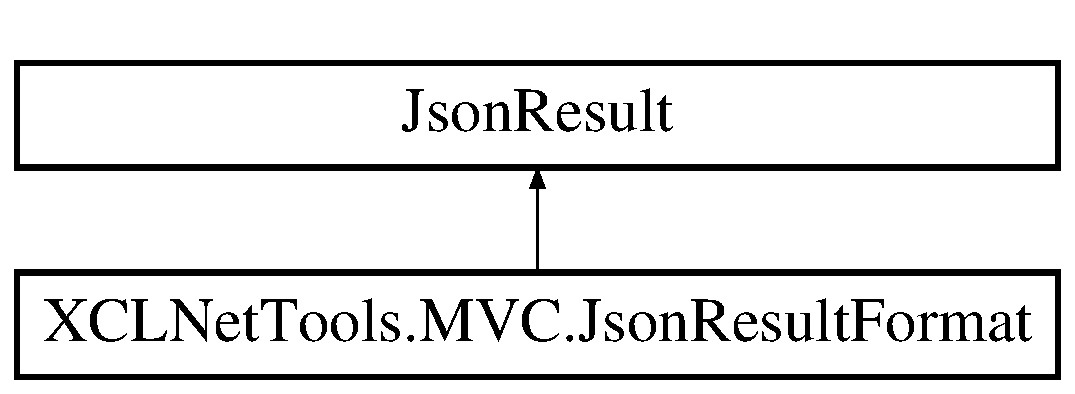
\includegraphics[height=2.000000cm]{class_x_c_l_net_tools_1_1_m_v_c_1_1_json_result_format}
\end{center}
\end{figure}
\subsection*{Public 成员函数}
\begin{DoxyCompactItemize}
\item 
override void \hyperlink{class_x_c_l_net_tools_1_1_m_v_c_1_1_json_result_format_aa8f3283c42c9130afd1aa8990876f413}{Execute\+Result} (Controller\+Context context)
\begin{DoxyCompactList}\small\item\em 重写执行视图 \end{DoxyCompactList}\end{DoxyCompactItemize}
\subsection*{属性}
\begin{DoxyCompactItemize}
\item 
string \hyperlink{class_x_c_l_net_tools_1_1_m_v_c_1_1_json_result_format_afc01b7cf2cd3f17c481c25ad70fcd4f6}{Date\+Format}\hspace{0.3cm}{\ttfamily  \mbox{[}get, set\mbox{]}}
\begin{DoxyCompactList}\small\item\em 格式化时间,默认值为\char`\"{}yyyy-\/\+M\+M-\/dd H\+H\+:mm\+:ss\char`\"{} \end{DoxyCompactList}\end{DoxyCompactItemize}


\subsection{详细描述}
带时间格式的json\+Result 



在文件 Json\+Result\+Format.\+cs 第 19 行定义.



\subsection{成员函数说明}
\index{X\+C\+L\+Net\+Tools\+::\+M\+V\+C\+::\+Json\+Result\+Format@{X\+C\+L\+Net\+Tools\+::\+M\+V\+C\+::\+Json\+Result\+Format}!Execute\+Result@{Execute\+Result}}
\index{Execute\+Result@{Execute\+Result}!X\+C\+L\+Net\+Tools\+::\+M\+V\+C\+::\+Json\+Result\+Format@{X\+C\+L\+Net\+Tools\+::\+M\+V\+C\+::\+Json\+Result\+Format}}
\subsubsection[{\texorpdfstring{Execute\+Result(\+Controller\+Context context)}{ExecuteResult(ControllerContext context)}}]{\setlength{\rightskip}{0pt plus 5cm}override void X\+C\+L\+Net\+Tools.\+M\+V\+C.\+Json\+Result\+Format.\+Execute\+Result (
\begin{DoxyParamCaption}
\item[{Controller\+Context}]{context}
\end{DoxyParamCaption}
)}\hypertarget{class_x_c_l_net_tools_1_1_m_v_c_1_1_json_result_format_aa8f3283c42c9130afd1aa8990876f413}{}\label{class_x_c_l_net_tools_1_1_m_v_c_1_1_json_result_format_aa8f3283c42c9130afd1aa8990876f413}


重写执行视图 


\begin{DoxyParams}{参数}
{\em context} & 上下文\\
\hline
\end{DoxyParams}


在文件 Json\+Result\+Format.\+cs 第 36 行定义.



\subsection{属性说明}
\index{X\+C\+L\+Net\+Tools\+::\+M\+V\+C\+::\+Json\+Result\+Format@{X\+C\+L\+Net\+Tools\+::\+M\+V\+C\+::\+Json\+Result\+Format}!Date\+Format@{Date\+Format}}
\index{Date\+Format@{Date\+Format}!X\+C\+L\+Net\+Tools\+::\+M\+V\+C\+::\+Json\+Result\+Format@{X\+C\+L\+Net\+Tools\+::\+M\+V\+C\+::\+Json\+Result\+Format}}
\subsubsection[{\texorpdfstring{Date\+Format}{DateFormat}}]{\setlength{\rightskip}{0pt plus 5cm}string X\+C\+L\+Net\+Tools.\+M\+V\+C.\+Json\+Result\+Format.\+Date\+Format\hspace{0.3cm}{\ttfamily [get]}, {\ttfamily [set]}}\hypertarget{class_x_c_l_net_tools_1_1_m_v_c_1_1_json_result_format_afc01b7cf2cd3f17c481c25ad70fcd4f6}{}\label{class_x_c_l_net_tools_1_1_m_v_c_1_1_json_result_format_afc01b7cf2cd3f17c481c25ad70fcd4f6}


格式化时间,默认值为\char`\"{}yyyy-\/\+M\+M-\/dd H\+H\+:mm\+:ss\char`\"{} 



在文件 Json\+Result\+Format.\+cs 第 27 行定义.



该类的文档由以下文件生成\+:\begin{DoxyCompactItemize}
\item 
E\+:/\+Git\+Hub/\+X\+C\+L\+Net\+Tools/\+X\+C\+L\+Net\+Tools/\+M\+V\+C/\hyperlink{_json_result_format_8cs}{Json\+Result\+Format.\+cs}\end{DoxyCompactItemize}

\hypertarget{class_x_c_l_net_tools_1_1_entity_1_1_key_value}{\section{X\-C\-L\-Net\-Tools.\-Entity.\-Key\-Value类 参考}
\label{class_x_c_l_net_tools_1_1_entity_1_1_key_value}\index{X\-C\-L\-Net\-Tools.\-Entity.\-Key\-Value@{X\-C\-L\-Net\-Tools.\-Entity.\-Key\-Value}}
}


键值类  


\subsection*{属性}
\begin{DoxyCompactItemize}
\item 
string \hyperlink{class_x_c_l_net_tools_1_1_entity_1_1_key_value_a33e2f7bfdcc6a1dce560304a4450cf08}{Key}\hspace{0.3cm}{\ttfamily  \mbox{[}get, set\mbox{]}}
\begin{DoxyCompactList}\small\item\em 键 \end{DoxyCompactList}\item 
string \hyperlink{class_x_c_l_net_tools_1_1_entity_1_1_key_value_a9ec3c76143930f64c1e0de2074514bae}{Value}\hspace{0.3cm}{\ttfamily  \mbox{[}get, set\mbox{]}}
\begin{DoxyCompactList}\small\item\em 值 \end{DoxyCompactList}\end{DoxyCompactItemize}


\subsection{详细描述}
键值类 



在文件 Key\-Value.\-cs 第 9 行定义.



\subsection{属性说明}
\hypertarget{class_x_c_l_net_tools_1_1_entity_1_1_key_value_a33e2f7bfdcc6a1dce560304a4450cf08}{\index{X\-C\-L\-Net\-Tools\-::\-Entity\-::\-Key\-Value@{X\-C\-L\-Net\-Tools\-::\-Entity\-::\-Key\-Value}!Key@{Key}}
\index{Key@{Key}!XCLNetTools::Entity::KeyValue@{X\-C\-L\-Net\-Tools\-::\-Entity\-::\-Key\-Value}}
\subsubsection[{Key}]{\setlength{\rightskip}{0pt plus 5cm}string X\-C\-L\-Net\-Tools.\-Entity.\-Key\-Value.\-Key\hspace{0.3cm}{\ttfamily [get]}, {\ttfamily [set]}}}\label{class_x_c_l_net_tools_1_1_entity_1_1_key_value_a33e2f7bfdcc6a1dce560304a4450cf08}


键 



在文件 Key\-Value.\-cs 第 14 行定义.

\hypertarget{class_x_c_l_net_tools_1_1_entity_1_1_key_value_a9ec3c76143930f64c1e0de2074514bae}{\index{X\-C\-L\-Net\-Tools\-::\-Entity\-::\-Key\-Value@{X\-C\-L\-Net\-Tools\-::\-Entity\-::\-Key\-Value}!Value@{Value}}
\index{Value@{Value}!XCLNetTools::Entity::KeyValue@{X\-C\-L\-Net\-Tools\-::\-Entity\-::\-Key\-Value}}
\subsubsection[{Value}]{\setlength{\rightskip}{0pt plus 5cm}string X\-C\-L\-Net\-Tools.\-Entity.\-Key\-Value.\-Value\hspace{0.3cm}{\ttfamily [get]}, {\ttfamily [set]}}}\label{class_x_c_l_net_tools_1_1_entity_1_1_key_value_a9ec3c76143930f64c1e0de2074514bae}


值 



在文件 Key\-Value.\-cs 第 19 行定义.



该类的文档由以下文件生成\-:\begin{DoxyCompactItemize}
\item 
Entity/\hyperlink{_key_value_8cs}{Key\-Value.\-cs}\end{DoxyCompactItemize}

\hypertarget{class_x_c_l_net_tools_1_1_serialize_1_1_lib}{}\section{X\+C\+L\+Net\+Tools.\+Serialize.\+Lib类 参考}
\label{class_x_c_l_net_tools_1_1_serialize_1_1_lib}\index{X\+C\+L\+Net\+Tools.\+Serialize.\+Lib@{X\+C\+L\+Net\+Tools.\+Serialize.\+Lib}}


其它对象序列化相关  


\subsection*{Public 成员函数}
\begin{DoxyCompactItemize}
\item 
T \hyperlink{class_x_c_l_net_tools_1_1_serialize_1_1_lib_ae2d400cea76a1f11f5141deab7c6d2b1}{Deserialize\+Object$<$ T $>$} (byte\mbox{[}$\,$\mbox{]} p\+Bytes)
\begin{DoxyCompactList}\small\item\em 把字节反序列化成相应的对象 \end{DoxyCompactList}\end{DoxyCompactItemize}
\subsection*{静态 Public 成员函数}
\begin{DoxyCompactItemize}
\item 
static T \hyperlink{class_x_c_l_net_tools_1_1_serialize_1_1_lib_ad38f60aaa57643027af6ebc86ef7fe18}{Deep\+Clone$<$ T $>$} (T source)
\begin{DoxyCompactList}\small\item\em 对象深度clone(被clone对象必须可以序列化) \end{DoxyCompactList}\item 
static Dictionary$<$ string, string $>$ \hyperlink{class_x_c_l_net_tools_1_1_serialize_1_1_lib_a99dccfb2469a4a61f20742a002a3f0ae}{Convert\+Json\+To\+Dictionary} (string json)
\begin{DoxyCompactList}\small\item\em 将\+J\+Object类型的属性转换为dictionary \end{DoxyCompactList}\item 
static string \hyperlink{class_x_c_l_net_tools_1_1_serialize_1_1_lib_a0034741d0598296a34082889f2a2f83e}{Convert\+Json\+To\+Url\+Parameters} (string json)
\begin{DoxyCompactList}\small\item\em 将\+J\+Object的属性转换为url参数形式 如:\{\char`\"{}a\char`\"{}\+:\char`\"{}1\char`\"{},\char`\"{}b\char`\"{}\+:\char`\"{}2\char`\"{},\char`\"{}c\char`\"{}\+:\{\char`\"{}d\char`\"{}\+:\char`\"{}100\char`\"{}\}\} -\/$>$ a=1\&b=2\&c.\+d=100 \end{DoxyCompactList}\end{DoxyCompactItemize}


\subsection{详细描述}
其它对象序列化相关 



在文件 Lib.\+cs 第 22 行定义.



\subsection{成员函数说明}
\mbox{\Hypertarget{class_x_c_l_net_tools_1_1_serialize_1_1_lib_a99dccfb2469a4a61f20742a002a3f0ae}\label{class_x_c_l_net_tools_1_1_serialize_1_1_lib_a99dccfb2469a4a61f20742a002a3f0ae}} 
\index{X\+C\+L\+Net\+Tools\+::\+Serialize\+::\+Lib@{X\+C\+L\+Net\+Tools\+::\+Serialize\+::\+Lib}!Convert\+Json\+To\+Dictionary@{Convert\+Json\+To\+Dictionary}}
\index{Convert\+Json\+To\+Dictionary@{Convert\+Json\+To\+Dictionary}!X\+C\+L\+Net\+Tools\+::\+Serialize\+::\+Lib@{X\+C\+L\+Net\+Tools\+::\+Serialize\+::\+Lib}}
\subsubsection{\texorpdfstring{Convert\+Json\+To\+Dictionary()}{ConvertJsonToDictionary()}}
{\footnotesize\ttfamily static Dictionary$<$string, string$>$ X\+C\+L\+Net\+Tools.\+Serialize.\+Lib.\+Convert\+Json\+To\+Dictionary (\begin{DoxyParamCaption}\item[{string}]{json }\end{DoxyParamCaption})\hspace{0.3cm}{\ttfamily [static]}}



将\+J\+Object类型的属性转换为dictionary 


\begin{DoxyParams}{参数}
{\em json} & 要转换的json\\
\hline
\end{DoxyParams}
\begin{DoxyReturn}{返回}
dictionary结果
\end{DoxyReturn}


在文件 Lib.\+cs 第 115 行定义.

\mbox{\Hypertarget{class_x_c_l_net_tools_1_1_serialize_1_1_lib_a0034741d0598296a34082889f2a2f83e}\label{class_x_c_l_net_tools_1_1_serialize_1_1_lib_a0034741d0598296a34082889f2a2f83e}} 
\index{X\+C\+L\+Net\+Tools\+::\+Serialize\+::\+Lib@{X\+C\+L\+Net\+Tools\+::\+Serialize\+::\+Lib}!Convert\+Json\+To\+Url\+Parameters@{Convert\+Json\+To\+Url\+Parameters}}
\index{Convert\+Json\+To\+Url\+Parameters@{Convert\+Json\+To\+Url\+Parameters}!X\+C\+L\+Net\+Tools\+::\+Serialize\+::\+Lib@{X\+C\+L\+Net\+Tools\+::\+Serialize\+::\+Lib}}
\subsubsection{\texorpdfstring{Convert\+Json\+To\+Url\+Parameters()}{ConvertJsonToUrlParameters()}}
{\footnotesize\ttfamily static string X\+C\+L\+Net\+Tools.\+Serialize.\+Lib.\+Convert\+Json\+To\+Url\+Parameters (\begin{DoxyParamCaption}\item[{string}]{json }\end{DoxyParamCaption})\hspace{0.3cm}{\ttfamily [static]}}



将\+J\+Object的属性转换为url参数形式 如:\{\char`\"{}a\char`\"{}\+:\char`\"{}1\char`\"{},\char`\"{}b\char`\"{}\+:\char`\"{}2\char`\"{},\char`\"{}c\char`\"{}\+:\{\char`\"{}d\char`\"{}\+:\char`\"{}100\char`\"{}\}\} -\/$>$ a=1\&b=2\&c.\+d=100 


\begin{DoxyParams}{参数}
{\em json} & 需要转换的json\\
\hline
\end{DoxyParams}
\begin{DoxyReturn}{返回}
url参数字符串
\end{DoxyReturn}


在文件 Lib.\+cs 第 136 行定义.

\mbox{\Hypertarget{class_x_c_l_net_tools_1_1_serialize_1_1_lib_ad38f60aaa57643027af6ebc86ef7fe18}\label{class_x_c_l_net_tools_1_1_serialize_1_1_lib_ad38f60aaa57643027af6ebc86ef7fe18}} 
\index{X\+C\+L\+Net\+Tools\+::\+Serialize\+::\+Lib@{X\+C\+L\+Net\+Tools\+::\+Serialize\+::\+Lib}!Deep\+Clone$<$ T $>$@{Deep\+Clone$<$ T $>$}}
\index{Deep\+Clone$<$ T $>$@{Deep\+Clone$<$ T $>$}!X\+C\+L\+Net\+Tools\+::\+Serialize\+::\+Lib@{X\+C\+L\+Net\+Tools\+::\+Serialize\+::\+Lib}}
\subsubsection{\texorpdfstring{Deep\+Clone$<$ T $>$()}{DeepClone< T >()}}
{\footnotesize\ttfamily static T X\+C\+L\+Net\+Tools.\+Serialize.\+Lib.\+Deep\+Clone$<$ T $>$ (\begin{DoxyParamCaption}\item[{T}]{source }\end{DoxyParamCaption})\hspace{0.3cm}{\ttfamily [static]}}



对象深度clone(被clone对象必须可以序列化) 


\begin{DoxyParams}{参数}
{\em source} & 要克隆的对象\\
\hline
\end{DoxyParams}
\begin{DoxyReturn}{返回}
克隆后的新对象
\end{DoxyReturn}
\begin{Desc}
\item[类型限制]\begin{description}
\item[{\em T} : {\em class}]\end{description}
\end{Desc}


在文件 Lib.\+cs 第 56 行定义.

\mbox{\Hypertarget{class_x_c_l_net_tools_1_1_serialize_1_1_lib_ae2d400cea76a1f11f5141deab7c6d2b1}\label{class_x_c_l_net_tools_1_1_serialize_1_1_lib_ae2d400cea76a1f11f5141deab7c6d2b1}} 
\index{X\+C\+L\+Net\+Tools\+::\+Serialize\+::\+Lib@{X\+C\+L\+Net\+Tools\+::\+Serialize\+::\+Lib}!Deserialize\+Object$<$ T $>$@{Deserialize\+Object$<$ T $>$}}
\index{Deserialize\+Object$<$ T $>$@{Deserialize\+Object$<$ T $>$}!X\+C\+L\+Net\+Tools\+::\+Serialize\+::\+Lib@{X\+C\+L\+Net\+Tools\+::\+Serialize\+::\+Lib}}
\subsubsection{\texorpdfstring{Deserialize\+Object$<$ T $>$()}{DeserializeObject< T >()}}
{\footnotesize\ttfamily T X\+C\+L\+Net\+Tools.\+Serialize.\+Lib.\+Deserialize\+Object$<$ T $>$ (\begin{DoxyParamCaption}\item[{byte \mbox{[}$\,$\mbox{]}}]{p\+Bytes }\end{DoxyParamCaption})}



把字节反序列化成相应的对象 


\begin{DoxyParams}{参数}
{\em p\+Bytes} & 字节流\\
\hline
\end{DoxyParams}
\begin{DoxyReturn}{返回}
T
\end{DoxyReturn}
\begin{Desc}
\item[类型限制]\begin{description}
\item[{\em T} : {\em class}]\end{description}
\end{Desc}


在文件 Lib.\+cs 第 31 行定义.



该类的文档由以下文件生成\+:\begin{DoxyCompactItemize}
\item 
D\+:/\+My\+Data/\+Git\+Hub/\+X\+C\+L\+Net\+Tools/\+X\+C\+L\+Net\+Tools/\+Serialize/\hyperlink{_serialize_2_lib_8cs}{Lib.\+cs}\end{DoxyCompactItemize}

\hypertarget{class_x_c_l_net_tools_1_1_control_1_1_html_control_1_1_lib}{\section{X\-C\-L\-Net\-Tools.\-Control.\-Html\-Control.\-Lib类 参考}
\label{class_x_c_l_net_tools_1_1_control_1_1_html_control_1_1_lib}\index{X\-C\-L\-Net\-Tools.\-Control.\-Html\-Control.\-Lib@{X\-C\-L\-Net\-Tools.\-Control.\-Html\-Control.\-Lib}}
}


原生html控件操作类  


\subsection*{静态 Public 成员函数}
\begin{DoxyCompactItemize}
\item 
static string \hyperlink{class_x_c_l_net_tools_1_1_control_1_1_html_control_1_1_lib_a6bc535ff27a3e67b2c4dac1d5e99aa8c}{Get\-Options} (Type t, \hyperlink{class_x_c_l_net_tools_1_1_entity_1_1_set_option_entity}{Set\-Option\-Entity} options=null)
\begin{DoxyCompactList}\small\item\em 将枚举转为select的options 
\begin{DoxyParams}{参数}
{\em t} & 枚举type\\
\hline
{\em options} & 选项\\
\hline
\end{DoxyParams}
\end{DoxyCompactList}\item 
static string \hyperlink{class_x_c_l_net_tools_1_1_control_1_1_html_control_1_1_lib_aea5ab0601c97a418ef6291f75aa7baff}{Get\-Options} (Dictionary$<$ string, string $>$ data\-Source, \hyperlink{class_x_c_l_net_tools_1_1_entity_1_1_set_option_entity}{Set\-Option\-Entity} options=null)
\begin{DoxyCompactList}\small\item\em 将\-Dictionary转为select 的options \end{DoxyCompactList}\end{DoxyCompactItemize}


\subsection{详细描述}
原生html控件操作类 



在文件 Lib.\-cs 第 32 行定义.



\subsection{成员函数说明}
\hypertarget{class_x_c_l_net_tools_1_1_control_1_1_html_control_1_1_lib_a6bc535ff27a3e67b2c4dac1d5e99aa8c}{\index{X\-C\-L\-Net\-Tools\-::\-Control\-::\-Html\-Control\-::\-Lib@{X\-C\-L\-Net\-Tools\-::\-Control\-::\-Html\-Control\-::\-Lib}!Get\-Options@{Get\-Options}}
\index{Get\-Options@{Get\-Options}!XCLNetTools::Control::HtmlControl::Lib@{X\-C\-L\-Net\-Tools\-::\-Control\-::\-Html\-Control\-::\-Lib}}
\subsubsection[{Get\-Options}]{\setlength{\rightskip}{0pt plus 5cm}static string X\-C\-L\-Net\-Tools.\-Control.\-Html\-Control.\-Lib.\-Get\-Options (
\begin{DoxyParamCaption}
\item[{Type}]{t, }
\item[{{\bf Set\-Option\-Entity}}]{options = {\ttfamily null}}
\end{DoxyParamCaption}
)\hspace{0.3cm}{\ttfamily [static]}}}\label{class_x_c_l_net_tools_1_1_control_1_1_html_control_1_1_lib_a6bc535ff27a3e67b2c4dac1d5e99aa8c}


将枚举转为select的options 
\begin{DoxyParams}{参数}
{\em t} & 枚举type\\
\hline
{\em options} & 选项\\
\hline
\end{DoxyParams}




在文件 Lib.\-cs 第 39 行定义.

\hypertarget{class_x_c_l_net_tools_1_1_control_1_1_html_control_1_1_lib_aea5ab0601c97a418ef6291f75aa7baff}{\index{X\-C\-L\-Net\-Tools\-::\-Control\-::\-Html\-Control\-::\-Lib@{X\-C\-L\-Net\-Tools\-::\-Control\-::\-Html\-Control\-::\-Lib}!Get\-Options@{Get\-Options}}
\index{Get\-Options@{Get\-Options}!XCLNetTools::Control::HtmlControl::Lib@{X\-C\-L\-Net\-Tools\-::\-Control\-::\-Html\-Control\-::\-Lib}}
\subsubsection[{Get\-Options}]{\setlength{\rightskip}{0pt plus 5cm}static string X\-C\-L\-Net\-Tools.\-Control.\-Html\-Control.\-Lib.\-Get\-Options (
\begin{DoxyParamCaption}
\item[{Dictionary$<$ string, string $>$}]{data\-Source, }
\item[{{\bf Set\-Option\-Entity}}]{options = {\ttfamily null}}
\end{DoxyParamCaption}
)\hspace{0.3cm}{\ttfamily [static]}}}\label{class_x_c_l_net_tools_1_1_control_1_1_html_control_1_1_lib_aea5ab0601c97a418ef6291f75aa7baff}


将\-Dictionary转为select 的options 


\begin{DoxyParams}{参数}
{\em data\-Source} & 数据源\\
\hline
{\em options} & 选项\\
\hline
\end{DoxyParams}


在文件 Lib.\-cs 第 69 行定义.



该类的文档由以下文件生成\-:\begin{DoxyCompactItemize}
\item 
D\-:/\-My\-Data/\-My\-Git/\-Git\-Hub/\-X\-C\-L\-Net\-Tools/\-X\-C\-L\-Net\-Tools/\-Control/\-Html\-Control/\hyperlink{_control_2_html_control_2_lib_8cs}{Lib.\-cs}\end{DoxyCompactItemize}

\hypertarget{class_x_c_l_net_tools_1_1_control_1_1_server_control_1_1_lib}{\section{X\-C\-L\-Net\-Tools.\-Control.\-Server\-Control.\-Lib类 参考}
\label{class_x_c_l_net_tools_1_1_control_1_1_server_control_1_1_lib}\index{X\-C\-L\-Net\-Tools.\-Control.\-Server\-Control.\-Lib@{X\-C\-L\-Net\-Tools.\-Control.\-Server\-Control.\-Lib}}
}


服务器控件操作相关  


\subsection*{静态 Public 成员函数}
\begin{DoxyCompactItemize}
\item 
static void \hyperlink{class_x_c_l_net_tools_1_1_control_1_1_server_control_1_1_lib_a788673e8352bff030ce50d1b42cfd44f}{Rep\-Data\-Bind$<$ T $>$} (Repeater rep, List$<$ T $>$ data\-Source, bool is\-Show\-No\-Data\-Msg, params string\mbox{[}$\,$\mbox{]} no\-Data\-Msg)
\begin{DoxyCompactList}\small\item\em Repeater绑定数据 \end{DoxyCompactList}\item 
static void \hyperlink{class_x_c_l_net_tools_1_1_control_1_1_server_control_1_1_lib_ad2856902e5c392c722a55c82d9977586}{Rep\-Data\-Bind} (Repeater rep, Data\-Table data\-Source, bool is\-Show\-No\-Data\-Msg, params string\mbox{[}$\,$\mbox{]} no\-Data\-Msg)
\begin{DoxyCompactList}\small\item\em Repeater绑定数据 \end{DoxyCompactList}\item 
static void \hyperlink{class_x_c_l_net_tools_1_1_control_1_1_server_control_1_1_lib_a7d5141c14830a52c7d4edcab2d104452}{Bind\-D\-D\-L} (System.\-Web.\-U\-I.\-Web\-Controls.\-Drop\-Down\-List ddl, Data\-Set ds, string text\-Field, string value\-Field, string value, bool flag)
\begin{DoxyCompactList}\small\item\em 绑定\-D\-D\-L,value为初始选中值 \end{DoxyCompactList}\item 
static void \hyperlink{class_x_c_l_net_tools_1_1_control_1_1_server_control_1_1_lib_af2a5dcd9fa457696d15a072e4772b861}{Bind\-Check\-Box\-List} (System.\-Web.\-U\-I.\-Web\-Controls.\-Check\-Box\-List ck, Data\-Set ds, string text\-Field, string value\-Field, string value)
\begin{DoxyCompactList}\small\item\em 绑定\-Check\-Box\-List,value为初始选中值 \end{DoxyCompactList}\item 
static void \hyperlink{class_x_c_l_net_tools_1_1_control_1_1_server_control_1_1_lib_acf0e494ba2e94742818fbebfd883ab17}{Bind\-Enum} (System.\-Web.\-U\-I.\-Web\-Controls.\-Web\-Control c, List$<$ \hyperlink{class_x_c_l_net_tools_1_1_entity_1_1_text_value}{X\-C\-L\-Net\-Tools.\-Entity.\-Text\-Value} $>$ lst, string default\-Value)
\begin{DoxyCompactList}\small\item\em 绑定枚举(此方法已过期,请使用\-Bind\-Lst) \end{DoxyCompactList}\item 
static void \hyperlink{class_x_c_l_net_tools_1_1_control_1_1_server_control_1_1_lib_ad5ebfd4eb97120e0049cd0260e150ed9}{Bind\-Lst$<$ T $>$} (System.\-Web.\-U\-I.\-Web\-Controls.\-Web\-Control c, List$<$ T $>$ lst, string text\-Field, string value\-Field, string value, bool flag)
\begin{DoxyCompactList}\small\item\em 将list绑定到控件上 \end{DoxyCompactList}\end{DoxyCompactItemize}


\subsection{详细描述}
服务器控件操作相关 



在文件 Lib.\-cs 第 35 行定义.



\subsection{成员函数说明}
\hypertarget{class_x_c_l_net_tools_1_1_control_1_1_server_control_1_1_lib_af2a5dcd9fa457696d15a072e4772b861}{\index{X\-C\-L\-Net\-Tools\-::\-Control\-::\-Server\-Control\-::\-Lib@{X\-C\-L\-Net\-Tools\-::\-Control\-::\-Server\-Control\-::\-Lib}!Bind\-Check\-Box\-List@{Bind\-Check\-Box\-List}}
\index{Bind\-Check\-Box\-List@{Bind\-Check\-Box\-List}!XCLNetTools::Control::ServerControl::Lib@{X\-C\-L\-Net\-Tools\-::\-Control\-::\-Server\-Control\-::\-Lib}}
\subsubsection[{Bind\-Check\-Box\-List}]{\setlength{\rightskip}{0pt plus 5cm}static void X\-C\-L\-Net\-Tools.\-Control.\-Server\-Control.\-Lib.\-Bind\-Check\-Box\-List (
\begin{DoxyParamCaption}
\item[{System.\-Web.\-U\-I.\-Web\-Controls.\-Check\-Box\-List}]{ck, }
\item[{Data\-Set}]{ds, }
\item[{string}]{text\-Field, }
\item[{string}]{value\-Field, }
\item[{string}]{value}
\end{DoxyParamCaption}
)\hspace{0.3cm}{\ttfamily [static]}}}\label{class_x_c_l_net_tools_1_1_control_1_1_server_control_1_1_lib_af2a5dcd9fa457696d15a072e4772b861}


绑定\-Check\-Box\-List,value为初始选中值 


\begin{DoxyParams}{参数}
{\em ck} & Check\-Box\-List\\
\hline
{\em ds} & dataset\\
\hline
{\em text\-Field} & 文本字段\\
\hline
{\em value\-Field} & 值字段\\
\hline
{\em value} & 以,隔开的字符串,默认选中值\\
\hline
\end{DoxyParams}


在文件 Lib.\-cs 第 131 行定义.

\hypertarget{class_x_c_l_net_tools_1_1_control_1_1_server_control_1_1_lib_a7d5141c14830a52c7d4edcab2d104452}{\index{X\-C\-L\-Net\-Tools\-::\-Control\-::\-Server\-Control\-::\-Lib@{X\-C\-L\-Net\-Tools\-::\-Control\-::\-Server\-Control\-::\-Lib}!Bind\-D\-D\-L@{Bind\-D\-D\-L}}
\index{Bind\-D\-D\-L@{Bind\-D\-D\-L}!XCLNetTools::Control::ServerControl::Lib@{X\-C\-L\-Net\-Tools\-::\-Control\-::\-Server\-Control\-::\-Lib}}
\subsubsection[{Bind\-D\-D\-L}]{\setlength{\rightskip}{0pt plus 5cm}static void X\-C\-L\-Net\-Tools.\-Control.\-Server\-Control.\-Lib.\-Bind\-D\-D\-L (
\begin{DoxyParamCaption}
\item[{System.\-Web.\-U\-I.\-Web\-Controls.\-Drop\-Down\-List}]{ddl, }
\item[{Data\-Set}]{ds, }
\item[{string}]{text\-Field, }
\item[{string}]{value\-Field, }
\item[{string}]{value, }
\item[{bool}]{flag}
\end{DoxyParamCaption}
)\hspace{0.3cm}{\ttfamily [static]}}}\label{class_x_c_l_net_tools_1_1_control_1_1_server_control_1_1_lib_a7d5141c14830a52c7d4edcab2d104452}


绑定\-D\-D\-L,value为初始选中值 


\begin{DoxyParams}{参数}
{\em ddl} & Drop\-Down\-List\\
\hline
{\em ds} & dataset\\
\hline
{\em text\-Field} & 文本字段\\
\hline
{\em value\-Field} & 值字段\\
\hline
{\em value} & 默认选中项的值\\
\hline
{\em flag} & true\-:有\char`\"{}-\/-\/全部-\/-\/\char`\"{} false\-:无\\
\hline
\end{DoxyParams}


在文件 Lib.\-cs 第 100 行定义.

\hypertarget{class_x_c_l_net_tools_1_1_control_1_1_server_control_1_1_lib_acf0e494ba2e94742818fbebfd883ab17}{\index{X\-C\-L\-Net\-Tools\-::\-Control\-::\-Server\-Control\-::\-Lib@{X\-C\-L\-Net\-Tools\-::\-Control\-::\-Server\-Control\-::\-Lib}!Bind\-Enum@{Bind\-Enum}}
\index{Bind\-Enum@{Bind\-Enum}!XCLNetTools::Control::ServerControl::Lib@{X\-C\-L\-Net\-Tools\-::\-Control\-::\-Server\-Control\-::\-Lib}}
\subsubsection[{Bind\-Enum}]{\setlength{\rightskip}{0pt plus 5cm}static void X\-C\-L\-Net\-Tools.\-Control.\-Server\-Control.\-Lib.\-Bind\-Enum (
\begin{DoxyParamCaption}
\item[{System.\-Web.\-U\-I.\-Web\-Controls.\-Web\-Control}]{c, }
\item[{List$<$ {\bf X\-C\-L\-Net\-Tools.\-Entity.\-Text\-Value} $>$}]{lst, }
\item[{string}]{default\-Value}
\end{DoxyParamCaption}
)\hspace{0.3cm}{\ttfamily [static]}}}\label{class_x_c_l_net_tools_1_1_control_1_1_server_control_1_1_lib_acf0e494ba2e94742818fbebfd883ab17}


绑定枚举(此方法已过期,请使用\-Bind\-Lst) 


\begin{DoxyParams}{参数}
{\em c} & 控件\\
\hline
{\em lst} & \hyperlink{class_x_c_l_net_tools_1_1_entity_1_1_text_value}{X\-C\-L\-Net\-Tools.\-Entity.\-Text\-Value} list\\
\hline
{\em default\-Value} & 默认选中值\\
\hline
\end{DoxyParams}


在文件 Lib.\-cs 第 168 行定义.

\hypertarget{class_x_c_l_net_tools_1_1_control_1_1_server_control_1_1_lib_ad5ebfd4eb97120e0049cd0260e150ed9}{\index{X\-C\-L\-Net\-Tools\-::\-Control\-::\-Server\-Control\-::\-Lib@{X\-C\-L\-Net\-Tools\-::\-Control\-::\-Server\-Control\-::\-Lib}!Bind\-Lst$<$ T $>$@{Bind\-Lst$<$ T $>$}}
\index{Bind\-Lst$<$ T $>$@{Bind\-Lst$<$ T $>$}!XCLNetTools::Control::ServerControl::Lib@{X\-C\-L\-Net\-Tools\-::\-Control\-::\-Server\-Control\-::\-Lib}}
\subsubsection[{Bind\-Lst$<$ T $>$}]{\setlength{\rightskip}{0pt plus 5cm}static void X\-C\-L\-Net\-Tools.\-Control.\-Server\-Control.\-Lib.\-Bind\-Lst$<$ T $>$ (
\begin{DoxyParamCaption}
\item[{System.\-Web.\-U\-I.\-Web\-Controls.\-Web\-Control}]{c, }
\item[{List$<$ T $>$}]{lst, }
\item[{string}]{text\-Field, }
\item[{string}]{value\-Field, }
\item[{string}]{value, }
\item[{bool}]{flag}
\end{DoxyParamCaption}
)\hspace{0.3cm}{\ttfamily [static]}}}\label{class_x_c_l_net_tools_1_1_control_1_1_server_control_1_1_lib_ad5ebfd4eb97120e0049cd0260e150ed9}


将list绑定到控件上 


\begin{DoxyParams}{参数}
{\em c} & 控件\\
\hline
{\em lst} & 数据源\\
\hline
{\em text\-Field} & 文本字段\\
\hline
{\em value\-Field} & 值字段\\
\hline
{\em value} & 选中值\\
\hline
{\em flag} & 第一项是否为\char`\"{}请选择\char`\"{}\\
\hline
\end{DoxyParams}


在文件 Lib.\-cs 第 196 行定义.

\hypertarget{class_x_c_l_net_tools_1_1_control_1_1_server_control_1_1_lib_ad2856902e5c392c722a55c82d9977586}{\index{X\-C\-L\-Net\-Tools\-::\-Control\-::\-Server\-Control\-::\-Lib@{X\-C\-L\-Net\-Tools\-::\-Control\-::\-Server\-Control\-::\-Lib}!Rep\-Data\-Bind@{Rep\-Data\-Bind}}
\index{Rep\-Data\-Bind@{Rep\-Data\-Bind}!XCLNetTools::Control::ServerControl::Lib@{X\-C\-L\-Net\-Tools\-::\-Control\-::\-Server\-Control\-::\-Lib}}
\subsubsection[{Rep\-Data\-Bind}]{\setlength{\rightskip}{0pt plus 5cm}static void X\-C\-L\-Net\-Tools.\-Control.\-Server\-Control.\-Lib.\-Rep\-Data\-Bind (
\begin{DoxyParamCaption}
\item[{Repeater}]{rep, }
\item[{Data\-Table}]{data\-Source, }
\item[{bool}]{is\-Show\-No\-Data\-Msg, }
\item[{params string\mbox{[}$\,$\mbox{]}}]{no\-Data\-Msg}
\end{DoxyParamCaption}
)\hspace{0.3cm}{\ttfamily [static]}}}\label{class_x_c_l_net_tools_1_1_control_1_1_server_control_1_1_lib_ad2856902e5c392c722a55c82d9977586}


Repeater绑定数据 


\begin{DoxyParams}{参数}
{\em rep} & Repeater控件\\
\hline
{\em data\-Source} & 数据源\\
\hline
{\em is\-Show\-No\-Data\-Msg} & true\-:没有数据时,显示“暂无数据”\\
\hline
{\em no\-Data\-Msg} & 没有数据时非默认提示\\
\hline
\end{DoxyParams}


在文件 Lib.\-cs 第 70 行定义.

\hypertarget{class_x_c_l_net_tools_1_1_control_1_1_server_control_1_1_lib_a788673e8352bff030ce50d1b42cfd44f}{\index{X\-C\-L\-Net\-Tools\-::\-Control\-::\-Server\-Control\-::\-Lib@{X\-C\-L\-Net\-Tools\-::\-Control\-::\-Server\-Control\-::\-Lib}!Rep\-Data\-Bind$<$ T $>$@{Rep\-Data\-Bind$<$ T $>$}}
\index{Rep\-Data\-Bind$<$ T $>$@{Rep\-Data\-Bind$<$ T $>$}!XCLNetTools::Control::ServerControl::Lib@{X\-C\-L\-Net\-Tools\-::\-Control\-::\-Server\-Control\-::\-Lib}}
\subsubsection[{Rep\-Data\-Bind$<$ T $>$}]{\setlength{\rightskip}{0pt plus 5cm}static void {\bf X\-C\-L\-Net\-Tools.\-Control.\-Server\-Control.\-Lib.\-Rep\-Data\-Bind}$<$ T $>$ (
\begin{DoxyParamCaption}
\item[{Repeater}]{rep, }
\item[{List$<$ T $>$}]{data\-Source, }
\item[{bool}]{is\-Show\-No\-Data\-Msg, }
\item[{params string\mbox{[}$\,$\mbox{]}}]{no\-Data\-Msg}
\end{DoxyParamCaption}
)\hspace{0.3cm}{\ttfamily [static]}}}\label{class_x_c_l_net_tools_1_1_control_1_1_server_control_1_1_lib_a788673e8352bff030ce50d1b42cfd44f}


Repeater绑定数据 


\begin{DoxyParams}{参数}
{\em rep} & Repeater控件\\
\hline
{\em data\-Source} & 数据源\\
\hline
{\em is\-Show\-No\-Data\-Msg} & true\-:没有数据时,显示“暂无数据”\\
\hline
{\em no\-Data\-Msg} & 没有数据时非默认提示\\
\hline
\end{DoxyParams}


在文件 Lib.\-cs 第 46 行定义.



该类的文档由以下文件生成\-:\begin{DoxyCompactItemize}
\item 
D\-:/\-My\-Data/\-My\-Git/\-Git\-Hub/\-X\-C\-L\-Net\-Tools/\-X\-C\-L\-Net\-Tools/\-Control/\-Server\-Control/\hyperlink{_control_2_server_control_2_lib_8cs}{Lib.\-cs}\end{DoxyCompactItemize}

\hypertarget{class_x_c_l_net_tools_1_1_control_1_1_mx_graph_1_1_lib}{}\section{X\+C\+L\+Net\+Tools.\+Control.\+Mx\+Graph.\+Lib类 参考}
\label{class_x_c_l_net_tools_1_1_control_1_1_mx_graph_1_1_lib}\index{X\+C\+L\+Net\+Tools.\+Control.\+Mx\+Graph.\+Lib@{X\+C\+L\+Net\+Tools.\+Control.\+Mx\+Graph.\+Lib}}


Mx\+Graph操作类  


\subsection*{静态 Public 成员函数}
\begin{DoxyCompactItemize}
\item 
static Image \hyperlink{class_x_c_l_net_tools_1_1_control_1_1_mx_graph_1_1_lib_abff455d51f61485d6bf26e0133af6000}{Get\+Image} (string xml)
\begin{DoxyCompactList}\small\item\em 根据view形式的xml生成图片 \end{DoxyCompactList}\item 
static void \hyperlink{class_x_c_l_net_tools_1_1_control_1_1_mx_graph_1_1_lib_ad6b09c60b11a1f51a6bf45cc3bde1b88}{Export\+Image} (string xml, string filename)
\begin{DoxyCompactList}\small\item\em 导出mx\+Graph为图片 \end{DoxyCompactList}\end{DoxyCompactItemize}


\subsection{详细描述}
Mx\+Graph操作类 



在文件 Lib.\+cs 第 22 行定义.



\subsection{成员函数说明}
\index{X\+C\+L\+Net\+Tools\+::\+Control\+::\+Mx\+Graph\+::\+Lib@{X\+C\+L\+Net\+Tools\+::\+Control\+::\+Mx\+Graph\+::\+Lib}!Export\+Image@{Export\+Image}}
\index{Export\+Image@{Export\+Image}!X\+C\+L\+Net\+Tools\+::\+Control\+::\+Mx\+Graph\+::\+Lib@{X\+C\+L\+Net\+Tools\+::\+Control\+::\+Mx\+Graph\+::\+Lib}}
\subsubsection[{\texorpdfstring{Export\+Image(string xml, string filename)}{ExportImage(string xml, string filename)}}]{\setlength{\rightskip}{0pt plus 5cm}static void X\+C\+L\+Net\+Tools.\+Control.\+Mx\+Graph.\+Lib.\+Export\+Image (
\begin{DoxyParamCaption}
\item[{string}]{xml, }
\item[{string}]{filename}
\end{DoxyParamCaption}
)\hspace{0.3cm}{\ttfamily [static]}}\hypertarget{class_x_c_l_net_tools_1_1_control_1_1_mx_graph_1_1_lib_ad6b09c60b11a1f51a6bf45cc3bde1b88}{}\label{class_x_c_l_net_tools_1_1_control_1_1_mx_graph_1_1_lib_ad6b09c60b11a1f51a6bf45cc3bde1b88}


导出mx\+Graph为图片 


\begin{DoxyParams}{参数}
{\em xml} & mx\+Graph的model的view形式的xml\\
\hline
{\em filename} & 导出后的文件名(包含扩展名)\\
\hline
\end{DoxyParams}


在文件 Lib.\+cs 第 45 行定义.

\index{X\+C\+L\+Net\+Tools\+::\+Control\+::\+Mx\+Graph\+::\+Lib@{X\+C\+L\+Net\+Tools\+::\+Control\+::\+Mx\+Graph\+::\+Lib}!Get\+Image@{Get\+Image}}
\index{Get\+Image@{Get\+Image}!X\+C\+L\+Net\+Tools\+::\+Control\+::\+Mx\+Graph\+::\+Lib@{X\+C\+L\+Net\+Tools\+::\+Control\+::\+Mx\+Graph\+::\+Lib}}
\subsubsection[{\texorpdfstring{Get\+Image(string xml)}{GetImage(string xml)}}]{\setlength{\rightskip}{0pt plus 5cm}static Image X\+C\+L\+Net\+Tools.\+Control.\+Mx\+Graph.\+Lib.\+Get\+Image (
\begin{DoxyParamCaption}
\item[{string}]{xml}
\end{DoxyParamCaption}
)\hspace{0.3cm}{\ttfamily [static]}}\hypertarget{class_x_c_l_net_tools_1_1_control_1_1_mx_graph_1_1_lib_abff455d51f61485d6bf26e0133af6000}{}\label{class_x_c_l_net_tools_1_1_control_1_1_mx_graph_1_1_lib_abff455d51f61485d6bf26e0133af6000}


根据view形式的xml生成图片 


\begin{DoxyParams}{参数}
{\em xml} & view形式的xml\\
\hline
\end{DoxyParams}
\begin{DoxyReturn}{返回}
image对象
\end{DoxyReturn}


在文件 Lib.\+cs 第 29 行定义.



该类的文档由以下文件生成\+:\begin{DoxyCompactItemize}
\item 
E\+:/\+Git\+Hub/\+X\+C\+L\+Net\+Tools/\+X\+C\+L\+Net\+Tools/\+Control/\+Mx\+Graph/\hyperlink{_control_2_mx_graph_2_lib_8cs}{Lib.\+cs}\end{DoxyCompactItemize}

\hypertarget{class_x_c_l_net_tools_1_1_encode_1_1_lib}{\section{X\-C\-L\-Net\-Tools.\-Encode.\-Lib类 参考}
\label{class_x_c_l_net_tools_1_1_encode_1_1_lib}\index{X\-C\-L\-Net\-Tools.\-Encode.\-Lib@{X\-C\-L\-Net\-Tools.\-Encode.\-Lib}}
}


其它相关  


\subsection*{静态 Public 成员函数}
\begin{DoxyCompactItemize}
\item 
static string \hyperlink{class_x_c_l_net_tools_1_1_encode_1_1_lib_a3820bb303f5c96fa7e802f4cd0ac9ece}{Unescape} (string str)
\begin{DoxyCompactList}\small\item\em 对js的escape进行解码 \end{DoxyCompactList}\end{DoxyCompactItemize}


\subsection{详细描述}
其它相关 



在文件 Lib.\-cs 第 27 行定义.



\subsection{成员函数说明}
\hypertarget{class_x_c_l_net_tools_1_1_encode_1_1_lib_a3820bb303f5c96fa7e802f4cd0ac9ece}{\index{X\-C\-L\-Net\-Tools\-::\-Encode\-::\-Lib@{X\-C\-L\-Net\-Tools\-::\-Encode\-::\-Lib}!Unescape@{Unescape}}
\index{Unescape@{Unescape}!XCLNetTools::Encode::Lib@{X\-C\-L\-Net\-Tools\-::\-Encode\-::\-Lib}}
\subsubsection[{Unescape}]{\setlength{\rightskip}{0pt plus 5cm}static string X\-C\-L\-Net\-Tools.\-Encode.\-Lib.\-Unescape (
\begin{DoxyParamCaption}
\item[{string}]{str}
\end{DoxyParamCaption}
)\hspace{0.3cm}{\ttfamily [static]}}}\label{class_x_c_l_net_tools_1_1_encode_1_1_lib_a3820bb303f5c96fa7e802f4cd0ac9ece}


对js的escape进行解码 


\begin{DoxyParams}{参数}
{\em str} & 解码字符串\\
\hline
\end{DoxyParams}


在文件 Lib.\-cs 第 33 行定义.



该类的文档由以下文件生成\-:\begin{DoxyCompactItemize}
\item 
D\-:/\-My\-Data/\-My\-Git/\-Git\-Hub/\-X\-C\-L\-Net\-Tools/\-X\-C\-L\-Net\-Tools/\-Encode/\hyperlink{_encode_2_lib_8cs}{Lib.\-cs}\end{DoxyCompactItemize}

\hypertarget{class_x_c_l_net_tools_1_1_generic_1_1_list_helper}{\section{X\-C\-L\-Net\-Tools.\-Generic.\-List\-Helper类 参考}
\label{class_x_c_l_net_tools_1_1_generic_1_1_list_helper}\index{X\-C\-L\-Net\-Tools.\-Generic.\-List\-Helper@{X\-C\-L\-Net\-Tools.\-Generic.\-List\-Helper}}
}


List操作类  


\subsection*{静态 Public 成员函数}
\begin{DoxyCompactItemize}
\item 
static List$<$ List$<$ T $>$ $>$ \hyperlink{class_x_c_l_net_tools_1_1_generic_1_1_list_helper_a38adb871b8752fb797795645625b7b4f}{Split\-List\-By\-Step$<$ T $>$} (int step, List$<$ T $>$ lst)
\begin{DoxyCompactList}\small\item\em 根据步长,将一个总\-List拆分为多个子\-List \end{DoxyCompactList}\item 
static string \hyperlink{class_x_c_l_net_tools_1_1_generic_1_1_list_helper_a02b07a0f7a7d4506c358650ba010f7d9}{Get\-String\-By\-List$<$ T $>$} (List$<$ T $>$ lst, string split\-Char)
\begin{DoxyCompactList}\small\item\em 将list中的项拼接字符串 \end{DoxyCompactList}\item 
static Data\-Table \hyperlink{class_x_c_l_net_tools_1_1_generic_1_1_list_helper_aabb9427ae92df2eb55b7ea300be149a9}{To\-Data\-Table$<$ T $>$} (I\-List$<$ T $>$ data)
\begin{DoxyCompactList}\small\item\em 将\-List转换成\-Data\-Table \end{DoxyCompactList}\item 
static I\-List$<$ T $>$ \hyperlink{class_x_c_l_net_tools_1_1_generic_1_1_list_helper_aa1d5d2843b5a105edf4eb8c160fcd016}{Data\-Table\-To\-List$<$ T $>$} (Data\-Table dt)
\begin{DoxyCompactList}\small\item\em 将data\-Table转为list \end{DoxyCompactList}\end{DoxyCompactItemize}


\subsection{详细描述}
List操作类 



在文件 List\-Helper.\-cs 第 32 行定义.



\subsection{成员函数说明}
\hypertarget{class_x_c_l_net_tools_1_1_generic_1_1_list_helper_aa1d5d2843b5a105edf4eb8c160fcd016}{\index{X\-C\-L\-Net\-Tools\-::\-Generic\-::\-List\-Helper@{X\-C\-L\-Net\-Tools\-::\-Generic\-::\-List\-Helper}!Data\-Table\-To\-List$<$ T $>$@{Data\-Table\-To\-List$<$ T $>$}}
\index{Data\-Table\-To\-List$<$ T $>$@{Data\-Table\-To\-List$<$ T $>$}!XCLNetTools::Generic::ListHelper@{X\-C\-L\-Net\-Tools\-::\-Generic\-::\-List\-Helper}}
\subsubsection[{Data\-Table\-To\-List$<$ T $>$}]{\setlength{\rightskip}{0pt plus 5cm}static I\-List$<$T$>$ X\-C\-L\-Net\-Tools.\-Generic.\-List\-Helper.\-Data\-Table\-To\-List$<$ T $>$ (
\begin{DoxyParamCaption}
\item[{Data\-Table}]{dt}
\end{DoxyParamCaption}
)\hspace{0.3cm}{\ttfamily [static]}}}\label{class_x_c_l_net_tools_1_1_generic_1_1_list_helper_aa1d5d2843b5a105edf4eb8c160fcd016}


将data\-Table转为list 


\begin{DoxyParams}{参数}
{\em dt} & \\
\hline
\end{DoxyParams}
\begin{DoxyReturn}{返回}

\end{DoxyReturn}
\begin{Desc}
\item[类型限制]\begin{description}
\item[{\em T} : {\em new()}]\end{description}
\end{Desc}


在文件 List\-Helper.\-cs 第 104 行定义.

\hypertarget{class_x_c_l_net_tools_1_1_generic_1_1_list_helper_a02b07a0f7a7d4506c358650ba010f7d9}{\index{X\-C\-L\-Net\-Tools\-::\-Generic\-::\-List\-Helper@{X\-C\-L\-Net\-Tools\-::\-Generic\-::\-List\-Helper}!Get\-String\-By\-List$<$ T $>$@{Get\-String\-By\-List$<$ T $>$}}
\index{Get\-String\-By\-List$<$ T $>$@{Get\-String\-By\-List$<$ T $>$}!XCLNetTools::Generic::ListHelper@{X\-C\-L\-Net\-Tools\-::\-Generic\-::\-List\-Helper}}
\subsubsection[{Get\-String\-By\-List$<$ T $>$}]{\setlength{\rightskip}{0pt plus 5cm}static string X\-C\-L\-Net\-Tools.\-Generic.\-List\-Helper.\-Get\-String\-By\-List$<$ T $>$ (
\begin{DoxyParamCaption}
\item[{List$<$ T $>$}]{lst, }
\item[{string}]{split\-Char}
\end{DoxyParamCaption}
)\hspace{0.3cm}{\ttfamily [static]}}}\label{class_x_c_l_net_tools_1_1_generic_1_1_list_helper_a02b07a0f7a7d4506c358650ba010f7d9}


将list中的项拼接字符串 


\begin{DoxyParams}{参数}
{\em lst} & 要操作的list\\
\hline
{\em split\-Char} & 分隔符\\
\hline
\end{DoxyParams}


在文件 List\-Helper.\-cs 第 65 行定义.

\hypertarget{class_x_c_l_net_tools_1_1_generic_1_1_list_helper_a38adb871b8752fb797795645625b7b4f}{\index{X\-C\-L\-Net\-Tools\-::\-Generic\-::\-List\-Helper@{X\-C\-L\-Net\-Tools\-::\-Generic\-::\-List\-Helper}!Split\-List\-By\-Step$<$ T $>$@{Split\-List\-By\-Step$<$ T $>$}}
\index{Split\-List\-By\-Step$<$ T $>$@{Split\-List\-By\-Step$<$ T $>$}!XCLNetTools::Generic::ListHelper@{X\-C\-L\-Net\-Tools\-::\-Generic\-::\-List\-Helper}}
\subsubsection[{Split\-List\-By\-Step$<$ T $>$}]{\setlength{\rightskip}{0pt plus 5cm}static List$<$List$<$T$>$ $>$ X\-C\-L\-Net\-Tools.\-Generic.\-List\-Helper.\-Split\-List\-By\-Step$<$ T $>$ (
\begin{DoxyParamCaption}
\item[{int}]{step, }
\item[{List$<$ T $>$}]{lst}
\end{DoxyParamCaption}
)\hspace{0.3cm}{\ttfamily [static]}}}\label{class_x_c_l_net_tools_1_1_generic_1_1_list_helper_a38adb871b8752fb797795645625b7b4f}


根据步长,将一个总\-List拆分为多个子\-List 


\begin{DoxyParams}{参数}
{\em step} & 每个子list最多的项数\\
\hline
{\em lst} & 主list\\
\hline
\end{DoxyParams}


在文件 List\-Helper.\-cs 第 39 行定义.

\hypertarget{class_x_c_l_net_tools_1_1_generic_1_1_list_helper_aabb9427ae92df2eb55b7ea300be149a9}{\index{X\-C\-L\-Net\-Tools\-::\-Generic\-::\-List\-Helper@{X\-C\-L\-Net\-Tools\-::\-Generic\-::\-List\-Helper}!To\-Data\-Table$<$ T $>$@{To\-Data\-Table$<$ T $>$}}
\index{To\-Data\-Table$<$ T $>$@{To\-Data\-Table$<$ T $>$}!XCLNetTools::Generic::ListHelper@{X\-C\-L\-Net\-Tools\-::\-Generic\-::\-List\-Helper}}
\subsubsection[{To\-Data\-Table$<$ T $>$}]{\setlength{\rightskip}{0pt plus 5cm}static Data\-Table X\-C\-L\-Net\-Tools.\-Generic.\-List\-Helper.\-To\-Data\-Table$<$ T $>$ (
\begin{DoxyParamCaption}
\item[{I\-List$<$ T $>$}]{data}
\end{DoxyParamCaption}
)\hspace{0.3cm}{\ttfamily [static]}}}\label{class_x_c_l_net_tools_1_1_generic_1_1_list_helper_aabb9427ae92df2eb55b7ea300be149a9}


将\-List转换成\-Data\-Table 



在文件 List\-Helper.\-cs 第 78 行定义.



该类的文档由以下文件生成\-:\begin{DoxyCompactItemize}
\item 
D\-:/\-My\-Data/\-My\-Git/\-Git\-Hub/\-X\-C\-L\-Net\-Tools/\-X\-C\-L\-Net\-Tools/\-Generic/\hyperlink{_list_helper_8cs}{List\-Helper.\-cs}\end{DoxyCompactItemize}

\hypertarget{class_x_c_l_net_tools_1_1_serialize_1_1_lit_json}{}\section{X\+C\+L\+Net\+Tools.\+Serialize.\+Lit\+Json类 参考}
\label{class_x_c_l_net_tools_1_1_serialize_1_1_lit_json}\index{X\+C\+L\+Net\+Tools.\+Serialize.\+Lit\+Json@{X\+C\+L\+Net\+Tools.\+Serialize.\+Lit\+Json}}


Lit\+Json帮助类  


\subsection*{静态 Public 成员函数}
\begin{DoxyCompactItemize}
\item 
static string \hyperlink{class_x_c_l_net_tools_1_1_serialize_1_1_lit_json_a81a2b398d509a227753a98e12a79674e}{Convert\+Object\+To\+Json} (object obj)
\begin{DoxyCompactList}\small\item\em 对象转为json \end{DoxyCompactList}\item 
static string \hyperlink{class_x_c_l_net_tools_1_1_serialize_1_1_lit_json_a8bd51fdf8d1e56bee3e72c165f4d34ae}{Convert\+Data\+Table\+To\+Array} (System.\+Data.\+Data\+Table dt)
\begin{DoxyCompactList}\small\item\em Data\+Table转为js的数组形式,若为空,则返回\mbox{[}\mbox{]} \end{DoxyCompactList}\item 
static string \hyperlink{class_x_c_l_net_tools_1_1_serialize_1_1_lit_json_a118c20cd6f5a519aa5061f1d95f13c94}{Convert\+Data\+Table\+To\+Json} (Data\+Table dt, string json\+Name)
\begin{DoxyCompactList}\small\item\em Data\+Table转为json \end{DoxyCompactList}\item 
static string \hyperlink{class_x_c_l_net_tools_1_1_serialize_1_1_lit_json_a62018ecad0868724f8c525f6633c2db1}{Convert\+Data\+Set\+To\+Array} (System.\+Data.\+Data\+Set ds)
\begin{DoxyCompactList}\small\item\em Data\+Set转为js的数组形式,若为空,则返回\mbox{[}\mbox{]} \end{DoxyCompactList}\item 
static string \hyperlink{class_x_c_l_net_tools_1_1_serialize_1_1_lit_json_afe0e32c9376fb1c7f2c222eb8cfdcc18}{Convert\+Data\+Set\+To\+Json} (Data\+Set ds, string json\+Name)
\begin{DoxyCompactList}\small\item\em Data\+Set转为json \end{DoxyCompactList}\item 
static string \hyperlink{class_x_c_l_net_tools_1_1_serialize_1_1_lit_json_a97544159631e77ad1e2ab7fba119fce4}{Convert\+List\+To\+Json$<$ T $>$} (I\+List$<$ T $>$ lst, string json\+Name)
\begin{DoxyCompactList}\small\item\em List转为json \end{DoxyCompactList}\item 
static string \hyperlink{class_x_c_l_net_tools_1_1_serialize_1_1_lit_json_aed2848556cf9cdac6abfa0718a9a7fa4}{Convert\+List\+To\+Array$<$ T $>$} (I\+List$<$ T $>$ lst)
\begin{DoxyCompactList}\small\item\em List转为数组,若为空,则直接返回\mbox{[}\mbox{]} \end{DoxyCompactList}\end{DoxyCompactItemize}


\subsection{详细描述}
Lit\+Json帮助类 



在文件 Lit\+Json.\+cs 第 20 行定义.



\subsection{成员函数说明}
\index{X\+C\+L\+Net\+Tools\+::\+Serialize\+::\+Lit\+Json@{X\+C\+L\+Net\+Tools\+::\+Serialize\+::\+Lit\+Json}!Convert\+Data\+Set\+To\+Array@{Convert\+Data\+Set\+To\+Array}}
\index{Convert\+Data\+Set\+To\+Array@{Convert\+Data\+Set\+To\+Array}!X\+C\+L\+Net\+Tools\+::\+Serialize\+::\+Lit\+Json@{X\+C\+L\+Net\+Tools\+::\+Serialize\+::\+Lit\+Json}}
\subsubsection[{\texorpdfstring{Convert\+Data\+Set\+To\+Array(\+System.\+Data.\+Data\+Set ds)}{ConvertDataSetToArray(System.Data.DataSet ds)}}]{\setlength{\rightskip}{0pt plus 5cm}static string X\+C\+L\+Net\+Tools.\+Serialize.\+Lit\+Json.\+Convert\+Data\+Set\+To\+Array (
\begin{DoxyParamCaption}
\item[{System.\+Data.\+Data\+Set}]{ds}
\end{DoxyParamCaption}
)\hspace{0.3cm}{\ttfamily [static]}}\hypertarget{class_x_c_l_net_tools_1_1_serialize_1_1_lit_json_a62018ecad0868724f8c525f6633c2db1}{}\label{class_x_c_l_net_tools_1_1_serialize_1_1_lit_json_a62018ecad0868724f8c525f6633c2db1}


Data\+Set转为js的数组形式,若为空,则返回\mbox{[}\mbox{]} 


\begin{DoxyParams}{参数}
{\em ds} & 数据源\\
\hline
\end{DoxyParams}
\begin{DoxyReturn}{返回}
json数组
\end{DoxyReturn}


在文件 Lit\+Json.\+cs 第 88 行定义.

\index{X\+C\+L\+Net\+Tools\+::\+Serialize\+::\+Lit\+Json@{X\+C\+L\+Net\+Tools\+::\+Serialize\+::\+Lit\+Json}!Convert\+Data\+Set\+To\+Json@{Convert\+Data\+Set\+To\+Json}}
\index{Convert\+Data\+Set\+To\+Json@{Convert\+Data\+Set\+To\+Json}!X\+C\+L\+Net\+Tools\+::\+Serialize\+::\+Lit\+Json@{X\+C\+L\+Net\+Tools\+::\+Serialize\+::\+Lit\+Json}}
\subsubsection[{\texorpdfstring{Convert\+Data\+Set\+To\+Json(\+Data\+Set ds, string json\+Name)}{ConvertDataSetToJson(DataSet ds, string jsonName)}}]{\setlength{\rightskip}{0pt plus 5cm}static string X\+C\+L\+Net\+Tools.\+Serialize.\+Lit\+Json.\+Convert\+Data\+Set\+To\+Json (
\begin{DoxyParamCaption}
\item[{Data\+Set}]{ds, }
\item[{string}]{json\+Name}
\end{DoxyParamCaption}
)\hspace{0.3cm}{\ttfamily [static]}}\hypertarget{class_x_c_l_net_tools_1_1_serialize_1_1_lit_json_afe0e32c9376fb1c7f2c222eb8cfdcc18}{}\label{class_x_c_l_net_tools_1_1_serialize_1_1_lit_json_afe0e32c9376fb1c7f2c222eb8cfdcc18}


Data\+Set转为json 


\begin{DoxyParams}{参数}
{\em ds} & 数据源\\
\hline
{\em json\+Name} & 指定json key名\\
\hline
\end{DoxyParams}
\begin{DoxyReturn}{返回}
json
\end{DoxyReturn}


在文件 Lit\+Json.\+cs 第 109 行定义.

\index{X\+C\+L\+Net\+Tools\+::\+Serialize\+::\+Lit\+Json@{X\+C\+L\+Net\+Tools\+::\+Serialize\+::\+Lit\+Json}!Convert\+Data\+Table\+To\+Array@{Convert\+Data\+Table\+To\+Array}}
\index{Convert\+Data\+Table\+To\+Array@{Convert\+Data\+Table\+To\+Array}!X\+C\+L\+Net\+Tools\+::\+Serialize\+::\+Lit\+Json@{X\+C\+L\+Net\+Tools\+::\+Serialize\+::\+Lit\+Json}}
\subsubsection[{\texorpdfstring{Convert\+Data\+Table\+To\+Array(\+System.\+Data.\+Data\+Table dt)}{ConvertDataTableToArray(System.Data.DataTable dt)}}]{\setlength{\rightskip}{0pt plus 5cm}static string X\+C\+L\+Net\+Tools.\+Serialize.\+Lit\+Json.\+Convert\+Data\+Table\+To\+Array (
\begin{DoxyParamCaption}
\item[{System.\+Data.\+Data\+Table}]{dt}
\end{DoxyParamCaption}
)\hspace{0.3cm}{\ttfamily [static]}}\hypertarget{class_x_c_l_net_tools_1_1_serialize_1_1_lit_json_a8bd51fdf8d1e56bee3e72c165f4d34ae}{}\label{class_x_c_l_net_tools_1_1_serialize_1_1_lit_json_a8bd51fdf8d1e56bee3e72c165f4d34ae}


Data\+Table转为js的数组形式,若为空,则返回\mbox{[}\mbox{]} 


\begin{DoxyParams}{参数}
{\em dt} & 要处理的数据\\
\hline
\end{DoxyParams}
\begin{DoxyReturn}{返回}
json数组
\end{DoxyReturn}


在文件 Lit\+Json.\+cs 第 39 行定义.

\index{X\+C\+L\+Net\+Tools\+::\+Serialize\+::\+Lit\+Json@{X\+C\+L\+Net\+Tools\+::\+Serialize\+::\+Lit\+Json}!Convert\+Data\+Table\+To\+Json@{Convert\+Data\+Table\+To\+Json}}
\index{Convert\+Data\+Table\+To\+Json@{Convert\+Data\+Table\+To\+Json}!X\+C\+L\+Net\+Tools\+::\+Serialize\+::\+Lit\+Json@{X\+C\+L\+Net\+Tools\+::\+Serialize\+::\+Lit\+Json}}
\subsubsection[{\texorpdfstring{Convert\+Data\+Table\+To\+Json(\+Data\+Table dt, string json\+Name)}{ConvertDataTableToJson(DataTable dt, string jsonName)}}]{\setlength{\rightskip}{0pt plus 5cm}static string X\+C\+L\+Net\+Tools.\+Serialize.\+Lit\+Json.\+Convert\+Data\+Table\+To\+Json (
\begin{DoxyParamCaption}
\item[{Data\+Table}]{dt, }
\item[{string}]{json\+Name}
\end{DoxyParamCaption}
)\hspace{0.3cm}{\ttfamily [static]}}\hypertarget{class_x_c_l_net_tools_1_1_serialize_1_1_lit_json_a118c20cd6f5a519aa5061f1d95f13c94}{}\label{class_x_c_l_net_tools_1_1_serialize_1_1_lit_json_a118c20cd6f5a519aa5061f1d95f13c94}


Data\+Table转为json 


\begin{DoxyParams}{参数}
{\em dt} & 数据源\\
\hline
{\em json\+Name} & 指定的json key名\\
\hline
\end{DoxyParams}
\begin{DoxyReturn}{返回}
json
\end{DoxyReturn}


在文件 Lit\+Json.\+cs 第 74 行定义.

\index{X\+C\+L\+Net\+Tools\+::\+Serialize\+::\+Lit\+Json@{X\+C\+L\+Net\+Tools\+::\+Serialize\+::\+Lit\+Json}!Convert\+List\+To\+Array$<$ T $>$@{Convert\+List\+To\+Array$<$ T $>$}}
\index{Convert\+List\+To\+Array$<$ T $>$@{Convert\+List\+To\+Array$<$ T $>$}!X\+C\+L\+Net\+Tools\+::\+Serialize\+::\+Lit\+Json@{X\+C\+L\+Net\+Tools\+::\+Serialize\+::\+Lit\+Json}}
\subsubsection[{\texorpdfstring{Convert\+List\+To\+Array$<$ T $>$(\+I\+List$<$ T $>$ lst)}{ConvertListToArray< T >(IList< T > lst)}}]{\setlength{\rightskip}{0pt plus 5cm}static string X\+C\+L\+Net\+Tools.\+Serialize.\+Lit\+Json.\+Convert\+List\+To\+Array$<$ T $>$ (
\begin{DoxyParamCaption}
\item[{I\+List$<$ T $>$}]{lst}
\end{DoxyParamCaption}
)\hspace{0.3cm}{\ttfamily [static]}}\hypertarget{class_x_c_l_net_tools_1_1_serialize_1_1_lit_json_aed2848556cf9cdac6abfa0718a9a7fa4}{}\label{class_x_c_l_net_tools_1_1_serialize_1_1_lit_json_aed2848556cf9cdac6abfa0718a9a7fa4}


List转为数组,若为空,则直接返回\mbox{[}\mbox{]} 


\begin{DoxyParams}{参数}
{\em lst} & 数据源\\
\hline
\end{DoxyParams}
\begin{DoxyReturn}{返回}
json数组
\end{DoxyReturn}


在文件 Lit\+Json.\+cs 第 134 行定义.

\index{X\+C\+L\+Net\+Tools\+::\+Serialize\+::\+Lit\+Json@{X\+C\+L\+Net\+Tools\+::\+Serialize\+::\+Lit\+Json}!Convert\+List\+To\+Json$<$ T $>$@{Convert\+List\+To\+Json$<$ T $>$}}
\index{Convert\+List\+To\+Json$<$ T $>$@{Convert\+List\+To\+Json$<$ T $>$}!X\+C\+L\+Net\+Tools\+::\+Serialize\+::\+Lit\+Json@{X\+C\+L\+Net\+Tools\+::\+Serialize\+::\+Lit\+Json}}
\subsubsection[{\texorpdfstring{Convert\+List\+To\+Json$<$ T $>$(\+I\+List$<$ T $>$ lst, string json\+Name)}{ConvertListToJson< T >(IList< T > lst, string jsonName)}}]{\setlength{\rightskip}{0pt plus 5cm}static string X\+C\+L\+Net\+Tools.\+Serialize.\+Lit\+Json.\+Convert\+List\+To\+Json$<$ T $>$ (
\begin{DoxyParamCaption}
\item[{I\+List$<$ T $>$}]{lst, }
\item[{string}]{json\+Name}
\end{DoxyParamCaption}
)\hspace{0.3cm}{\ttfamily [static]}}\hypertarget{class_x_c_l_net_tools_1_1_serialize_1_1_lit_json_a97544159631e77ad1e2ab7fba119fce4}{}\label{class_x_c_l_net_tools_1_1_serialize_1_1_lit_json_a97544159631e77ad1e2ab7fba119fce4}


List转为json 


\begin{DoxyParams}{参数}
{\em lst} & 数据源\\
\hline
{\em json\+Name} & 指定json key名\\
\hline
\end{DoxyParams}
\begin{DoxyReturn}{返回}
json
\end{DoxyReturn}


在文件 Lit\+Json.\+cs 第 124 行定义.

\index{X\+C\+L\+Net\+Tools\+::\+Serialize\+::\+Lit\+Json@{X\+C\+L\+Net\+Tools\+::\+Serialize\+::\+Lit\+Json}!Convert\+Object\+To\+Json@{Convert\+Object\+To\+Json}}
\index{Convert\+Object\+To\+Json@{Convert\+Object\+To\+Json}!X\+C\+L\+Net\+Tools\+::\+Serialize\+::\+Lit\+Json@{X\+C\+L\+Net\+Tools\+::\+Serialize\+::\+Lit\+Json}}
\subsubsection[{\texorpdfstring{Convert\+Object\+To\+Json(object obj)}{ConvertObjectToJson(object obj)}}]{\setlength{\rightskip}{0pt plus 5cm}static string X\+C\+L\+Net\+Tools.\+Serialize.\+Lit\+Json.\+Convert\+Object\+To\+Json (
\begin{DoxyParamCaption}
\item[{object}]{obj}
\end{DoxyParamCaption}
)\hspace{0.3cm}{\ttfamily [static]}}\hypertarget{class_x_c_l_net_tools_1_1_serialize_1_1_lit_json_a81a2b398d509a227753a98e12a79674e}{}\label{class_x_c_l_net_tools_1_1_serialize_1_1_lit_json_a81a2b398d509a227753a98e12a79674e}


对象转为json 


\begin{DoxyParams}{参数}
{\em obj} & 要序列化的对象\\
\hline
\end{DoxyParams}
\begin{DoxyReturn}{返回}
json
\end{DoxyReturn}


在文件 Lit\+Json.\+cs 第 27 行定义.



该类的文档由以下文件生成\+:\begin{DoxyCompactItemize}
\item 
E\+:/\+Git\+Hub/\+X\+C\+L\+Net\+Tools/\+X\+C\+L\+Net\+Tools/\+Serialize/\hyperlink{_lit_json_8cs}{Lit\+Json.\+cs}\end{DoxyCompactItemize}

\hypertarget{class_x_c_l_net_tools_1_1_message_1_1_log}{\section{X\-C\-L\-Net\-Tools.\-Message.\-Log类 参考}
\label{class_x_c_l_net_tools_1_1_message_1_1_log}\index{X\-C\-L\-Net\-Tools.\-Message.\-Log@{X\-C\-L\-Net\-Tools.\-Message.\-Log}}
}


消息日志  


\subsection*{静态 Public 成员函数}
\begin{DoxyCompactItemize}
\item 
static void \hyperlink{class_x_c_l_net_tools_1_1_message_1_1_log_aac683d4043b6c9ac98f74d5f95dfa6f0}{Write\-Message} (object obj)
\begin{DoxyCompactList}\small\item\em 直接输出obj的json形式 \end{DoxyCompactList}\item 
static void \hyperlink{class_x_c_l_net_tools_1_1_message_1_1_log_a6038d85fedb63a3fe5dc306f1bf30011}{Write\-Message} (\hyperlink{class_x_c_l_net_tools_1_1_message_1_1_message_model}{Message\-Model} model)
\begin{DoxyCompactList}\small\item\em 直接输出\-Message\-Model的\-J\-S\-O\-N形式(此\-J\-S\-O\-N作为\-Log.\-Json\-Message\-Name的一个属性) \end{DoxyCompactList}\item 
static void \hyperlink{class_x_c_l_net_tools_1_1_message_1_1_log_a0f758d51c0cf8dd92645d44f1773715c}{Write\-Message} (string message)
\begin{DoxyCompactList}\small\item\em 输出消息(json) \hyperlink{class_x_c_l_net_tools_1_1_message_1_1_message_model}{Message\-Model} \end{DoxyCompactList}\end{DoxyCompactItemize}
\subsection*{静态 Public 属性}
\begin{DoxyCompactItemize}
\item 
static string \hyperlink{class_x_c_l_net_tools_1_1_message_1_1_log_ac9218999b3da2b5fbd7476e1ae47ca71}{Json\-Message\-Name} = string.\-Format(\char`\"{}X\-C\-L\{0\}\char`\"{}, X\-C\-L\-Net\-Tools.\-String\-Hander.\-Random\-Helper.\-Generate\-Id\-With\-Guid())
\begin{DoxyCompactList}\small\item\em 以json方式提示的属性名,它的下面有多个成员(如:data.\-Json\-Message\-Name.\-Message) \end{DoxyCompactList}\item 
static Action$<$ \hyperlink{class_x_c_l_net_tools_1_1_message_1_1_message_model}{Message\-Model} $>$ \hyperlink{class_x_c_l_net_tools_1_1_message_1_1_log_aeb571cf7294cbdc7776e44c5654b28d4}{Log\-Application\-Error\-Action} = new Action$<$\hyperlink{class_x_c_l_net_tools_1_1_message_1_1_message_model}{Message\-Model}$>$((msg\-Model) =$>$ \{ \hyperlink{class_x_c_l_net_tools_1_1_message_1_1_log_aac683d4043b6c9ac98f74d5f95dfa6f0}{X\-C\-L\-Net\-Tools.\-Message.\-Log.\-Write\-Message}(msg\-Model); \})
\begin{DoxyCompactList}\small\item\em 记录application error的处理方法,默认直接输出json \end{DoxyCompactList}\end{DoxyCompactItemize}


\subsection{详细描述}
消息日志 



在文件 Log.\-cs 第 17 行定义.



\subsection{成员函数说明}
\hypertarget{class_x_c_l_net_tools_1_1_message_1_1_log_aac683d4043b6c9ac98f74d5f95dfa6f0}{\index{X\-C\-L\-Net\-Tools\-::\-Message\-::\-Log@{X\-C\-L\-Net\-Tools\-::\-Message\-::\-Log}!Write\-Message@{Write\-Message}}
\index{Write\-Message@{Write\-Message}!XCLNetTools::Message::Log@{X\-C\-L\-Net\-Tools\-::\-Message\-::\-Log}}
\subsubsection[{Write\-Message}]{\setlength{\rightskip}{0pt plus 5cm}static void X\-C\-L\-Net\-Tools.\-Message.\-Log.\-Write\-Message (
\begin{DoxyParamCaption}
\item[{object}]{obj}
\end{DoxyParamCaption}
)\hspace{0.3cm}{\ttfamily [static]}}}\label{class_x_c_l_net_tools_1_1_message_1_1_log_aac683d4043b6c9ac98f74d5f95dfa6f0}


直接输出obj的json形式 


\begin{DoxyParams}{参数}
{\em obj} & 要输出的对象\\
\hline
\end{DoxyParams}


在文件 Log.\-cs 第 33 行定义.

\hypertarget{class_x_c_l_net_tools_1_1_message_1_1_log_a6038d85fedb63a3fe5dc306f1bf30011}{\index{X\-C\-L\-Net\-Tools\-::\-Message\-::\-Log@{X\-C\-L\-Net\-Tools\-::\-Message\-::\-Log}!Write\-Message@{Write\-Message}}
\index{Write\-Message@{Write\-Message}!XCLNetTools::Message::Log@{X\-C\-L\-Net\-Tools\-::\-Message\-::\-Log}}
\subsubsection[{Write\-Message}]{\setlength{\rightskip}{0pt plus 5cm}static void X\-C\-L\-Net\-Tools.\-Message.\-Log.\-Write\-Message (
\begin{DoxyParamCaption}
\item[{{\bf Message\-Model}}]{model}
\end{DoxyParamCaption}
)\hspace{0.3cm}{\ttfamily [static]}}}\label{class_x_c_l_net_tools_1_1_message_1_1_log_a6038d85fedb63a3fe5dc306f1bf30011}


直接输出\-Message\-Model的\-J\-S\-O\-N形式(此\-J\-S\-O\-N作为\-Log.\-Json\-Message\-Name的一个属性) 


\begin{DoxyParams}{参数}
{\em model} & 消息对象\\
\hline
\end{DoxyParams}


在文件 Log.\-cs 第 45 行定义.

\hypertarget{class_x_c_l_net_tools_1_1_message_1_1_log_a0f758d51c0cf8dd92645d44f1773715c}{\index{X\-C\-L\-Net\-Tools\-::\-Message\-::\-Log@{X\-C\-L\-Net\-Tools\-::\-Message\-::\-Log}!Write\-Message@{Write\-Message}}
\index{Write\-Message@{Write\-Message}!XCLNetTools::Message::Log@{X\-C\-L\-Net\-Tools\-::\-Message\-::\-Log}}
\subsubsection[{Write\-Message}]{\setlength{\rightskip}{0pt plus 5cm}static void X\-C\-L\-Net\-Tools.\-Message.\-Log.\-Write\-Message (
\begin{DoxyParamCaption}
\item[{string}]{message}
\end{DoxyParamCaption}
)\hspace{0.3cm}{\ttfamily [static]}}}\label{class_x_c_l_net_tools_1_1_message_1_1_log_a0f758d51c0cf8dd92645d44f1773715c}


输出消息(json) \hyperlink{class_x_c_l_net_tools_1_1_message_1_1_message_model}{Message\-Model} 


\begin{DoxyParams}{参数}
{\em message} & 消息\\
\hline
\end{DoxyParams}


在文件 Log.\-cs 第 59 行定义.



\subsection{类成员变量说明}
\hypertarget{class_x_c_l_net_tools_1_1_message_1_1_log_ac9218999b3da2b5fbd7476e1ae47ca71}{\index{X\-C\-L\-Net\-Tools\-::\-Message\-::\-Log@{X\-C\-L\-Net\-Tools\-::\-Message\-::\-Log}!Json\-Message\-Name@{Json\-Message\-Name}}
\index{Json\-Message\-Name@{Json\-Message\-Name}!XCLNetTools::Message::Log@{X\-C\-L\-Net\-Tools\-::\-Message\-::\-Log}}
\subsubsection[{Json\-Message\-Name}]{\setlength{\rightskip}{0pt plus 5cm}string X\-C\-L\-Net\-Tools.\-Message.\-Log.\-Json\-Message\-Name = string.\-Format(\char`\"{}X\-C\-L\{0\}\char`\"{}, X\-C\-L\-Net\-Tools.\-String\-Hander.\-Random\-Helper.\-Generate\-Id\-With\-Guid())\hspace{0.3cm}{\ttfamily [static]}}}\label{class_x_c_l_net_tools_1_1_message_1_1_log_ac9218999b3da2b5fbd7476e1ae47ca71}


以json方式提示的属性名,它的下面有多个成员(如:data.\-Json\-Message\-Name.\-Message) 



在文件 Log.\-cs 第 22 行定义.

\hypertarget{class_x_c_l_net_tools_1_1_message_1_1_log_aeb571cf7294cbdc7776e44c5654b28d4}{\index{X\-C\-L\-Net\-Tools\-::\-Message\-::\-Log@{X\-C\-L\-Net\-Tools\-::\-Message\-::\-Log}!Log\-Application\-Error\-Action@{Log\-Application\-Error\-Action}}
\index{Log\-Application\-Error\-Action@{Log\-Application\-Error\-Action}!XCLNetTools::Message::Log@{X\-C\-L\-Net\-Tools\-::\-Message\-::\-Log}}
\subsubsection[{Log\-Application\-Error\-Action}]{\setlength{\rightskip}{0pt plus 5cm}Action$<${\bf Message\-Model}$>$ X\-C\-L\-Net\-Tools.\-Message.\-Log.\-Log\-Application\-Error\-Action = new Action$<${\bf Message\-Model}$>$((msg\-Model) =$>$ \{ {\bf X\-C\-L\-Net\-Tools.\-Message.\-Log.\-Write\-Message}(msg\-Model); \})\hspace{0.3cm}{\ttfamily [static]}}}\label{class_x_c_l_net_tools_1_1_message_1_1_log_aeb571cf7294cbdc7776e44c5654b28d4}


记录application error的处理方法,默认直接输出json 



在文件 Log.\-cs 第 27 行定义.



该类的文档由以下文件生成\-:\begin{DoxyCompactItemize}
\item 
D\-:/\-My\-Data/\-My\-Git/\-Git\-Hub/\-X\-C\-L\-Net\-Tools/\-X\-C\-L\-Net\-Tools/\-Message/\hyperlink{_log_8cs}{Log.\-cs}\end{DoxyCompactItemize}

\hypertarget{class_x_c_l_net_tools_1_1_encrypt_1_1_m_d5}{}\section{X\+C\+L\+Net\+Tools.\+Encrypt.\+M\+D5类 参考}
\label{class_x_c_l_net_tools_1_1_encrypt_1_1_m_d5}\index{X\+C\+L\+Net\+Tools.\+Encrypt.\+M\+D5@{X\+C\+L\+Net\+Tools.\+Encrypt.\+M\+D5}}


md5相关  


\subsection*{静态 Public 成员函数}
\begin{DoxyCompactItemize}
\item 
static string \hyperlink{class_x_c_l_net_tools_1_1_encrypt_1_1_m_d5_a146cf118c47e0693f82119d39f4b7ef1}{Encode\+M\+D5} (string str, string key=\char`\"{}\char`\"{})
\begin{DoxyCompactList}\small\item\em M\+D5加密(大写) 
\begin{DoxyParams}{参数}
{\em str} & 待加密字符串\\
\hline
{\em key} & 是否在待加密的字符串中末尾追加该key,从而生成md5\\
\hline
\end{DoxyParams}
\begin{DoxyReturn}{返回}
加密后的字符串(大写)
\end{DoxyReturn}
\end{DoxyCompactList}\item 
static bool \hyperlink{class_x_c_l_net_tools_1_1_encrypt_1_1_m_d5_a47f3bda0226d74bd2c9823a023ed8ed5}{Is\+Equal\+M\+D5} (string str, string md5\+Str, string key=\char`\"{}\char`\"{})
\begin{DoxyCompactList}\small\item\em 判断明文与密文是否匹配 如果指定了key,则将明文与key组成的字符串的md5与md5\+Str进行比较 \end{DoxyCompactList}\end{DoxyCompactItemize}


\subsection{详细描述}
md5相关 



在文件 M\+D5.\+cs 第 16 行定义.



\subsection{成员函数说明}
\index{X\+C\+L\+Net\+Tools\+::\+Encrypt\+::\+M\+D5@{X\+C\+L\+Net\+Tools\+::\+Encrypt\+::\+M\+D5}!Encode\+M\+D5@{Encode\+M\+D5}}
\index{Encode\+M\+D5@{Encode\+M\+D5}!X\+C\+L\+Net\+Tools\+::\+Encrypt\+::\+M\+D5@{X\+C\+L\+Net\+Tools\+::\+Encrypt\+::\+M\+D5}}
\subsubsection[{\texorpdfstring{Encode\+M\+D5(string str, string key="""")}{EncodeMD5(string str, string key="")}}]{\setlength{\rightskip}{0pt plus 5cm}static string X\+C\+L\+Net\+Tools.\+Encrypt.\+M\+D5.\+Encode\+M\+D5 (
\begin{DoxyParamCaption}
\item[{string}]{str, }
\item[{string}]{key = {\ttfamily \char`\"{}\char`\"{}}}
\end{DoxyParamCaption}
)\hspace{0.3cm}{\ttfamily [static]}}\hypertarget{class_x_c_l_net_tools_1_1_encrypt_1_1_m_d5_a146cf118c47e0693f82119d39f4b7ef1}{}\label{class_x_c_l_net_tools_1_1_encrypt_1_1_m_d5_a146cf118c47e0693f82119d39f4b7ef1}


M\+D5加密(大写) 
\begin{DoxyParams}{参数}
{\em str} & 待加密字符串\\
\hline
{\em key} & 是否在待加密的字符串中末尾追加该key,从而生成md5\\
\hline
\end{DoxyParams}
\begin{DoxyReturn}{返回}
加密后的字符串(大写)
\end{DoxyReturn}




在文件 M\+D5.\+cs 第 24 行定义.

\index{X\+C\+L\+Net\+Tools\+::\+Encrypt\+::\+M\+D5@{X\+C\+L\+Net\+Tools\+::\+Encrypt\+::\+M\+D5}!Is\+Equal\+M\+D5@{Is\+Equal\+M\+D5}}
\index{Is\+Equal\+M\+D5@{Is\+Equal\+M\+D5}!X\+C\+L\+Net\+Tools\+::\+Encrypt\+::\+M\+D5@{X\+C\+L\+Net\+Tools\+::\+Encrypt\+::\+M\+D5}}
\subsubsection[{\texorpdfstring{Is\+Equal\+M\+D5(string str, string md5\+Str, string key="""")}{IsEqualMD5(string str, string md5Str, string key="")}}]{\setlength{\rightskip}{0pt plus 5cm}static bool X\+C\+L\+Net\+Tools.\+Encrypt.\+M\+D5.\+Is\+Equal\+M\+D5 (
\begin{DoxyParamCaption}
\item[{string}]{str, }
\item[{string}]{md5\+Str, }
\item[{string}]{key = {\ttfamily \char`\"{}\char`\"{}}}
\end{DoxyParamCaption}
)\hspace{0.3cm}{\ttfamily [static]}}\hypertarget{class_x_c_l_net_tools_1_1_encrypt_1_1_m_d5_a47f3bda0226d74bd2c9823a023ed8ed5}{}\label{class_x_c_l_net_tools_1_1_encrypt_1_1_m_d5_a47f3bda0226d74bd2c9823a023ed8ed5}


判断明文与密文是否匹配 如果指定了key,则将明文与key组成的字符串的md5与md5\+Str进行比较 


\begin{DoxyParams}{参数}
{\em str} & 明文\\
\hline
{\em md5\+Str} & md5密文\\
\hline
{\em key} & key\\
\hline
\end{DoxyParams}
\begin{DoxyReturn}{返回}
是否匹配
\end{DoxyReturn}


在文件 M\+D5.\+cs 第 37 行定义.



该类的文档由以下文件生成\+:\begin{DoxyCompactItemize}
\item 
E\+:/\+Git\+Hub/\+X\+C\+L\+Net\+Tools/\+X\+C\+L\+Net\+Tools/\+Encrypt/\hyperlink{_m_d5_8cs}{M\+D5.\+cs}\end{DoxyCompactItemize}

\hypertarget{class_x_c_l_net_tools_1_1_message_1_1_message_model}{}\section{X\+C\+L\+Net\+Tools.\+Message.\+Message\+Model类 参考}
\label{class_x_c_l_net_tools_1_1_message_1_1_message_model}\index{X\+C\+L\+Net\+Tools.\+Message.\+Message\+Model@{X\+C\+L\+Net\+Tools.\+Message.\+Message\+Model}}


消息提示实体类(用于json属性)  


\subsection*{属性}
\begin{DoxyCompactItemize}
\item 
virtual string \hyperlink{class_x_c_l_net_tools_1_1_message_1_1_message_model_a2347b5cf1ac7736de79aa94abd252d85}{Title}\hspace{0.3cm}{\ttfamily  \mbox{[}get, set\mbox{]}}
\begin{DoxyCompactList}\small\item\em 提示标题 \end{DoxyCompactList}\item 
virtual Date\+Time \hyperlink{class_x_c_l_net_tools_1_1_message_1_1_message_model_a04ede00490c3dbabea1fc01e6150715a}{Date}\hspace{0.3cm}{\ttfamily  \mbox{[}get, set\mbox{]}}
\begin{DoxyCompactList}\small\item\em 消息提示时间 \end{DoxyCompactList}\item 
virtual string \hyperlink{class_x_c_l_net_tools_1_1_message_1_1_message_model_a1fb1dde64c832e59d688d9a9fe944da5}{Message}\hspace{0.3cm}{\ttfamily  \mbox{[}get, set\mbox{]}}
\begin{DoxyCompactList}\small\item\em 消息提示内容 \end{DoxyCompactList}\item 
virtual string \hyperlink{class_x_c_l_net_tools_1_1_message_1_1_message_model_ae30c575345756a20443bb2f26ecdf1e9}{Message\+More}\hspace{0.3cm}{\ttfamily  \mbox{[}get, set\mbox{]}}
\begin{DoxyCompactList}\small\item\em 消息详细信息 \end{DoxyCompactList}\item 
virtual string \hyperlink{class_x_c_l_net_tools_1_1_message_1_1_message_model_a35cd14fdd9bbc8dea4c151c00d538755}{Url}\hspace{0.3cm}{\ttfamily  \mbox{[}get, set\mbox{]}}
\begin{DoxyCompactList}\small\item\em 消息发生页地址 \end{DoxyCompactList}\item 
virtual string \hyperlink{class_x_c_l_net_tools_1_1_message_1_1_message_model_a36e0a2784c189c86b33b76ceca539a28}{From\+Url}\hspace{0.3cm}{\ttfamily  \mbox{[}get, set\mbox{]}}
\begin{DoxyCompactList}\small\item\em 消息页来源地址(reffer) \end{DoxyCompactList}\item 
virtual bool \hyperlink{class_x_c_l_net_tools_1_1_message_1_1_message_model_a3881fb689ec30bfd21672b010a130675}{Is\+Success}\hspace{0.3cm}{\ttfamily  \mbox{[}get, set\mbox{]}}
\begin{DoxyCompactList}\small\item\em 是否成功与失败的标识 \end{DoxyCompactList}\item 
virtual bool \hyperlink{class_x_c_l_net_tools_1_1_message_1_1_message_model_a07c51819ac5836a7839b778c2cc62ba5}{Is\+Refresh}\hspace{0.3cm}{\ttfamily  \mbox{[}get, set\mbox{]}}
\begin{DoxyCompactList}\small\item\em 是否需要刷新 \end{DoxyCompactList}\item 
virtual string \hyperlink{class_x_c_l_net_tools_1_1_message_1_1_message_model_a933d98b3a93f2aefeaaf2d66940133a9}{Remark}\hspace{0.3cm}{\ttfamily  \mbox{[}get, set\mbox{]}}
\begin{DoxyCompactList}\small\item\em 备注信息 \end{DoxyCompactList}\item 
virtual bool \hyperlink{class_x_c_l_net_tools_1_1_message_1_1_message_model_af7a1590f9d2745c3db1486cb39edc070}{Is\+Redirect}\hspace{0.3cm}{\ttfamily  \mbox{[}get, set\mbox{]}}
\begin{DoxyCompactList}\small\item\em 是否需要跳转 \end{DoxyCompactList}\item 
virtual string \hyperlink{class_x_c_l_net_tools_1_1_message_1_1_message_model_a571c6e0204605733f900eb3f906e038d}{Redirect\+U\+RL}\hspace{0.3cm}{\ttfamily  \mbox{[}get, set\mbox{]}}
\begin{DoxyCompactList}\small\item\em 要跳转的url \end{DoxyCompactList}\item 
virtual \hyperlink{class_x_c_l_net_tools_1_1_enum_1_1_common_enum_a1cd31513e5ecf78c77d76be7954ae2f4}{X\+C\+L\+Net\+Tools.\+Enum.\+Common\+Enum.\+Redirect\+Target\+Enum} \hyperlink{class_x_c_l_net_tools_1_1_message_1_1_message_model_a318553f7c9db2b2c685e4944feb2901e}{Redirect\+Target}\hspace{0.3cm}{\ttfamily  \mbox{[}get, set\mbox{]}}
\begin{DoxyCompactList}\small\item\em 跳转方式 \end{DoxyCompactList}\item 
virtual bool \hyperlink{class_x_c_l_net_tools_1_1_message_1_1_message_model_a1ea24cc20f05516f6266af92cc06479a}{Is\+Ajax}\hspace{0.3cm}{\ttfamily  \mbox{[}get\mbox{]}}
\begin{DoxyCompactList}\small\item\em 当前请求是否为ajax请求 \end{DoxyCompactList}\item 
virtual string \hyperlink{class_x_c_l_net_tools_1_1_message_1_1_message_model_ab169d7bab20868e935d775459b72e625}{Error\+Code}\hspace{0.3cm}{\ttfamily  \mbox{[}get, set\mbox{]}}
\begin{DoxyCompactList}\small\item\em 错误码 \end{DoxyCompactList}\item 
virtual object \hyperlink{class_x_c_l_net_tools_1_1_message_1_1_message_model_a8065226d89965a09b9ff8e69ba9974ca}{Custom\+Object}\hspace{0.3cm}{\ttfamily  \mbox{[}get, set\mbox{]}}
\begin{DoxyCompactList}\small\item\em 自定义输出对象 \end{DoxyCompactList}\item 
virtual bool \hyperlink{class_x_c_l_net_tools_1_1_message_1_1_message_model_a2978a2953053a69008890758e419a1b3}{Is\+Exception}\hspace{0.3cm}{\ttfamily  \mbox{[}get, set\mbox{]}}
\begin{DoxyCompactList}\small\item\em 是否为异常 \end{DoxyCompactList}\end{DoxyCompactItemize}


\subsection{详细描述}
消息提示实体类(用于json属性) 



在文件 Message\+Model.\+cs 第 19 行定义.



\subsection{属性说明}
\mbox{\Hypertarget{class_x_c_l_net_tools_1_1_message_1_1_message_model_a8065226d89965a09b9ff8e69ba9974ca}\label{class_x_c_l_net_tools_1_1_message_1_1_message_model_a8065226d89965a09b9ff8e69ba9974ca}} 
\index{X\+C\+L\+Net\+Tools\+::\+Message\+::\+Message\+Model@{X\+C\+L\+Net\+Tools\+::\+Message\+::\+Message\+Model}!Custom\+Object@{Custom\+Object}}
\index{Custom\+Object@{Custom\+Object}!X\+C\+L\+Net\+Tools\+::\+Message\+::\+Message\+Model@{X\+C\+L\+Net\+Tools\+::\+Message\+::\+Message\+Model}}
\subsubsection{\texorpdfstring{Custom\+Object}{CustomObject}}
{\footnotesize\ttfamily virtual object X\+C\+L\+Net\+Tools.\+Message.\+Message\+Model.\+Custom\+Object\hspace{0.3cm}{\ttfamily [get]}, {\ttfamily [set]}}



自定义输出对象 



在文件 Message\+Model.\+cs 第 115 行定义.

\mbox{\Hypertarget{class_x_c_l_net_tools_1_1_message_1_1_message_model_a04ede00490c3dbabea1fc01e6150715a}\label{class_x_c_l_net_tools_1_1_message_1_1_message_model_a04ede00490c3dbabea1fc01e6150715a}} 
\index{X\+C\+L\+Net\+Tools\+::\+Message\+::\+Message\+Model@{X\+C\+L\+Net\+Tools\+::\+Message\+::\+Message\+Model}!Date@{Date}}
\index{Date@{Date}!X\+C\+L\+Net\+Tools\+::\+Message\+::\+Message\+Model@{X\+C\+L\+Net\+Tools\+::\+Message\+::\+Message\+Model}}
\subsubsection{\texorpdfstring{Date}{Date}}
{\footnotesize\ttfamily virtual Date\+Time X\+C\+L\+Net\+Tools.\+Message.\+Message\+Model.\+Date\hspace{0.3cm}{\ttfamily [get]}, {\ttfamily [set]}}



消息提示时间 



在文件 Message\+Model.\+cs 第 31 行定义.

\mbox{\Hypertarget{class_x_c_l_net_tools_1_1_message_1_1_message_model_ab169d7bab20868e935d775459b72e625}\label{class_x_c_l_net_tools_1_1_message_1_1_message_model_ab169d7bab20868e935d775459b72e625}} 
\index{X\+C\+L\+Net\+Tools\+::\+Message\+::\+Message\+Model@{X\+C\+L\+Net\+Tools\+::\+Message\+::\+Message\+Model}!Error\+Code@{Error\+Code}}
\index{Error\+Code@{Error\+Code}!X\+C\+L\+Net\+Tools\+::\+Message\+::\+Message\+Model@{X\+C\+L\+Net\+Tools\+::\+Message\+::\+Message\+Model}}
\subsubsection{\texorpdfstring{Error\+Code}{ErrorCode}}
{\footnotesize\ttfamily virtual string X\+C\+L\+Net\+Tools.\+Message.\+Message\+Model.\+Error\+Code\hspace{0.3cm}{\ttfamily [get]}, {\ttfamily [set]}}



错误码 



在文件 Message\+Model.\+cs 第 109 行定义.

\mbox{\Hypertarget{class_x_c_l_net_tools_1_1_message_1_1_message_model_a36e0a2784c189c86b33b76ceca539a28}\label{class_x_c_l_net_tools_1_1_message_1_1_message_model_a36e0a2784c189c86b33b76ceca539a28}} 
\index{X\+C\+L\+Net\+Tools\+::\+Message\+::\+Message\+Model@{X\+C\+L\+Net\+Tools\+::\+Message\+::\+Message\+Model}!From\+Url@{From\+Url}}
\index{From\+Url@{From\+Url}!X\+C\+L\+Net\+Tools\+::\+Message\+::\+Message\+Model@{X\+C\+L\+Net\+Tools\+::\+Message\+::\+Message\+Model}}
\subsubsection{\texorpdfstring{From\+Url}{FromUrl}}
{\footnotesize\ttfamily virtual string X\+C\+L\+Net\+Tools.\+Message.\+Message\+Model.\+From\+Url\hspace{0.3cm}{\ttfamily [get]}, {\ttfamily [set]}}



消息页来源地址(reffer) 



在文件 Message\+Model.\+cs 第 55 行定义.

\mbox{\Hypertarget{class_x_c_l_net_tools_1_1_message_1_1_message_model_a1ea24cc20f05516f6266af92cc06479a}\label{class_x_c_l_net_tools_1_1_message_1_1_message_model_a1ea24cc20f05516f6266af92cc06479a}} 
\index{X\+C\+L\+Net\+Tools\+::\+Message\+::\+Message\+Model@{X\+C\+L\+Net\+Tools\+::\+Message\+::\+Message\+Model}!Is\+Ajax@{Is\+Ajax}}
\index{Is\+Ajax@{Is\+Ajax}!X\+C\+L\+Net\+Tools\+::\+Message\+::\+Message\+Model@{X\+C\+L\+Net\+Tools\+::\+Message\+::\+Message\+Model}}
\subsubsection{\texorpdfstring{Is\+Ajax}{IsAjax}}
{\footnotesize\ttfamily virtual bool X\+C\+L\+Net\+Tools.\+Message.\+Message\+Model.\+Is\+Ajax\hspace{0.3cm}{\ttfamily [get]}}



当前请求是否为ajax请求 



在文件 Message\+Model.\+cs 第 98 行定义.

\mbox{\Hypertarget{class_x_c_l_net_tools_1_1_message_1_1_message_model_a2978a2953053a69008890758e419a1b3}\label{class_x_c_l_net_tools_1_1_message_1_1_message_model_a2978a2953053a69008890758e419a1b3}} 
\index{X\+C\+L\+Net\+Tools\+::\+Message\+::\+Message\+Model@{X\+C\+L\+Net\+Tools\+::\+Message\+::\+Message\+Model}!Is\+Exception@{Is\+Exception}}
\index{Is\+Exception@{Is\+Exception}!X\+C\+L\+Net\+Tools\+::\+Message\+::\+Message\+Model@{X\+C\+L\+Net\+Tools\+::\+Message\+::\+Message\+Model}}
\subsubsection{\texorpdfstring{Is\+Exception}{IsException}}
{\footnotesize\ttfamily virtual bool X\+C\+L\+Net\+Tools.\+Message.\+Message\+Model.\+Is\+Exception\hspace{0.3cm}{\ttfamily [get]}, {\ttfamily [set]}}



是否为异常 



在文件 Message\+Model.\+cs 第 121 行定义.

\mbox{\Hypertarget{class_x_c_l_net_tools_1_1_message_1_1_message_model_af7a1590f9d2745c3db1486cb39edc070}\label{class_x_c_l_net_tools_1_1_message_1_1_message_model_af7a1590f9d2745c3db1486cb39edc070}} 
\index{X\+C\+L\+Net\+Tools\+::\+Message\+::\+Message\+Model@{X\+C\+L\+Net\+Tools\+::\+Message\+::\+Message\+Model}!Is\+Redirect@{Is\+Redirect}}
\index{Is\+Redirect@{Is\+Redirect}!X\+C\+L\+Net\+Tools\+::\+Message\+::\+Message\+Model@{X\+C\+L\+Net\+Tools\+::\+Message\+::\+Message\+Model}}
\subsubsection{\texorpdfstring{Is\+Redirect}{IsRedirect}}
{\footnotesize\ttfamily virtual bool X\+C\+L\+Net\+Tools.\+Message.\+Message\+Model.\+Is\+Redirect\hspace{0.3cm}{\ttfamily [get]}, {\ttfamily [set]}}



是否需要跳转 



在文件 Message\+Model.\+cs 第 79 行定义.

\mbox{\Hypertarget{class_x_c_l_net_tools_1_1_message_1_1_message_model_a07c51819ac5836a7839b778c2cc62ba5}\label{class_x_c_l_net_tools_1_1_message_1_1_message_model_a07c51819ac5836a7839b778c2cc62ba5}} 
\index{X\+C\+L\+Net\+Tools\+::\+Message\+::\+Message\+Model@{X\+C\+L\+Net\+Tools\+::\+Message\+::\+Message\+Model}!Is\+Refresh@{Is\+Refresh}}
\index{Is\+Refresh@{Is\+Refresh}!X\+C\+L\+Net\+Tools\+::\+Message\+::\+Message\+Model@{X\+C\+L\+Net\+Tools\+::\+Message\+::\+Message\+Model}}
\subsubsection{\texorpdfstring{Is\+Refresh}{IsRefresh}}
{\footnotesize\ttfamily virtual bool X\+C\+L\+Net\+Tools.\+Message.\+Message\+Model.\+Is\+Refresh\hspace{0.3cm}{\ttfamily [get]}, {\ttfamily [set]}}



是否需要刷新 



在文件 Message\+Model.\+cs 第 67 行定义.

\mbox{\Hypertarget{class_x_c_l_net_tools_1_1_message_1_1_message_model_a3881fb689ec30bfd21672b010a130675}\label{class_x_c_l_net_tools_1_1_message_1_1_message_model_a3881fb689ec30bfd21672b010a130675}} 
\index{X\+C\+L\+Net\+Tools\+::\+Message\+::\+Message\+Model@{X\+C\+L\+Net\+Tools\+::\+Message\+::\+Message\+Model}!Is\+Success@{Is\+Success}}
\index{Is\+Success@{Is\+Success}!X\+C\+L\+Net\+Tools\+::\+Message\+::\+Message\+Model@{X\+C\+L\+Net\+Tools\+::\+Message\+::\+Message\+Model}}
\subsubsection{\texorpdfstring{Is\+Success}{IsSuccess}}
{\footnotesize\ttfamily virtual bool X\+C\+L\+Net\+Tools.\+Message.\+Message\+Model.\+Is\+Success\hspace{0.3cm}{\ttfamily [get]}, {\ttfamily [set]}}



是否成功与失败的标识 



在文件 Message\+Model.\+cs 第 61 行定义.

\mbox{\Hypertarget{class_x_c_l_net_tools_1_1_message_1_1_message_model_a1fb1dde64c832e59d688d9a9fe944da5}\label{class_x_c_l_net_tools_1_1_message_1_1_message_model_a1fb1dde64c832e59d688d9a9fe944da5}} 
\index{X\+C\+L\+Net\+Tools\+::\+Message\+::\+Message\+Model@{X\+C\+L\+Net\+Tools\+::\+Message\+::\+Message\+Model}!Message@{Message}}
\index{Message@{Message}!X\+C\+L\+Net\+Tools\+::\+Message\+::\+Message\+Model@{X\+C\+L\+Net\+Tools\+::\+Message\+::\+Message\+Model}}
\subsubsection{\texorpdfstring{Message}{Message}}
{\footnotesize\ttfamily virtual string X\+C\+L\+Net\+Tools.\+Message.\+Message\+Model.\+Message\hspace{0.3cm}{\ttfamily [get]}, {\ttfamily [set]}}



消息提示内容 



在文件 Message\+Model.\+cs 第 37 行定义.

\mbox{\Hypertarget{class_x_c_l_net_tools_1_1_message_1_1_message_model_ae30c575345756a20443bb2f26ecdf1e9}\label{class_x_c_l_net_tools_1_1_message_1_1_message_model_ae30c575345756a20443bb2f26ecdf1e9}} 
\index{X\+C\+L\+Net\+Tools\+::\+Message\+::\+Message\+Model@{X\+C\+L\+Net\+Tools\+::\+Message\+::\+Message\+Model}!Message\+More@{Message\+More}}
\index{Message\+More@{Message\+More}!X\+C\+L\+Net\+Tools\+::\+Message\+::\+Message\+Model@{X\+C\+L\+Net\+Tools\+::\+Message\+::\+Message\+Model}}
\subsubsection{\texorpdfstring{Message\+More}{MessageMore}}
{\footnotesize\ttfamily virtual string X\+C\+L\+Net\+Tools.\+Message.\+Message\+Model.\+Message\+More\hspace{0.3cm}{\ttfamily [get]}, {\ttfamily [set]}}



消息详细信息 



在文件 Message\+Model.\+cs 第 43 行定义.

\mbox{\Hypertarget{class_x_c_l_net_tools_1_1_message_1_1_message_model_a318553f7c9db2b2c685e4944feb2901e}\label{class_x_c_l_net_tools_1_1_message_1_1_message_model_a318553f7c9db2b2c685e4944feb2901e}} 
\index{X\+C\+L\+Net\+Tools\+::\+Message\+::\+Message\+Model@{X\+C\+L\+Net\+Tools\+::\+Message\+::\+Message\+Model}!Redirect\+Target@{Redirect\+Target}}
\index{Redirect\+Target@{Redirect\+Target}!X\+C\+L\+Net\+Tools\+::\+Message\+::\+Message\+Model@{X\+C\+L\+Net\+Tools\+::\+Message\+::\+Message\+Model}}
\subsubsection{\texorpdfstring{Redirect\+Target}{RedirectTarget}}
{\footnotesize\ttfamily virtual \hyperlink{class_x_c_l_net_tools_1_1_enum_1_1_common_enum_a1cd31513e5ecf78c77d76be7954ae2f4}{X\+C\+L\+Net\+Tools.\+Enum.\+Common\+Enum.\+Redirect\+Target\+Enum} X\+C\+L\+Net\+Tools.\+Message.\+Message\+Model.\+Redirect\+Target\hspace{0.3cm}{\ttfamily [get]}, {\ttfamily [set]}}



跳转方式 



在文件 Message\+Model.\+cs 第 91 行定义.

\mbox{\Hypertarget{class_x_c_l_net_tools_1_1_message_1_1_message_model_a571c6e0204605733f900eb3f906e038d}\label{class_x_c_l_net_tools_1_1_message_1_1_message_model_a571c6e0204605733f900eb3f906e038d}} 
\index{X\+C\+L\+Net\+Tools\+::\+Message\+::\+Message\+Model@{X\+C\+L\+Net\+Tools\+::\+Message\+::\+Message\+Model}!Redirect\+U\+RL@{Redirect\+U\+RL}}
\index{Redirect\+U\+RL@{Redirect\+U\+RL}!X\+C\+L\+Net\+Tools\+::\+Message\+::\+Message\+Model@{X\+C\+L\+Net\+Tools\+::\+Message\+::\+Message\+Model}}
\subsubsection{\texorpdfstring{Redirect\+U\+RL}{RedirectURL}}
{\footnotesize\ttfamily virtual string X\+C\+L\+Net\+Tools.\+Message.\+Message\+Model.\+Redirect\+U\+RL\hspace{0.3cm}{\ttfamily [get]}, {\ttfamily [set]}}



要跳转的url 



在文件 Message\+Model.\+cs 第 85 行定义.

\mbox{\Hypertarget{class_x_c_l_net_tools_1_1_message_1_1_message_model_a933d98b3a93f2aefeaaf2d66940133a9}\label{class_x_c_l_net_tools_1_1_message_1_1_message_model_a933d98b3a93f2aefeaaf2d66940133a9}} 
\index{X\+C\+L\+Net\+Tools\+::\+Message\+::\+Message\+Model@{X\+C\+L\+Net\+Tools\+::\+Message\+::\+Message\+Model}!Remark@{Remark}}
\index{Remark@{Remark}!X\+C\+L\+Net\+Tools\+::\+Message\+::\+Message\+Model@{X\+C\+L\+Net\+Tools\+::\+Message\+::\+Message\+Model}}
\subsubsection{\texorpdfstring{Remark}{Remark}}
{\footnotesize\ttfamily virtual string X\+C\+L\+Net\+Tools.\+Message.\+Message\+Model.\+Remark\hspace{0.3cm}{\ttfamily [get]}, {\ttfamily [set]}}



备注信息 



在文件 Message\+Model.\+cs 第 73 行定义.

\mbox{\Hypertarget{class_x_c_l_net_tools_1_1_message_1_1_message_model_a2347b5cf1ac7736de79aa94abd252d85}\label{class_x_c_l_net_tools_1_1_message_1_1_message_model_a2347b5cf1ac7736de79aa94abd252d85}} 
\index{X\+C\+L\+Net\+Tools\+::\+Message\+::\+Message\+Model@{X\+C\+L\+Net\+Tools\+::\+Message\+::\+Message\+Model}!Title@{Title}}
\index{Title@{Title}!X\+C\+L\+Net\+Tools\+::\+Message\+::\+Message\+Model@{X\+C\+L\+Net\+Tools\+::\+Message\+::\+Message\+Model}}
\subsubsection{\texorpdfstring{Title}{Title}}
{\footnotesize\ttfamily virtual string X\+C\+L\+Net\+Tools.\+Message.\+Message\+Model.\+Title\hspace{0.3cm}{\ttfamily [get]}, {\ttfamily [set]}}



提示标题 



在文件 Message\+Model.\+cs 第 25 行定义.

\mbox{\Hypertarget{class_x_c_l_net_tools_1_1_message_1_1_message_model_a35cd14fdd9bbc8dea4c151c00d538755}\label{class_x_c_l_net_tools_1_1_message_1_1_message_model_a35cd14fdd9bbc8dea4c151c00d538755}} 
\index{X\+C\+L\+Net\+Tools\+::\+Message\+::\+Message\+Model@{X\+C\+L\+Net\+Tools\+::\+Message\+::\+Message\+Model}!Url@{Url}}
\index{Url@{Url}!X\+C\+L\+Net\+Tools\+::\+Message\+::\+Message\+Model@{X\+C\+L\+Net\+Tools\+::\+Message\+::\+Message\+Model}}
\subsubsection{\texorpdfstring{Url}{Url}}
{\footnotesize\ttfamily virtual string X\+C\+L\+Net\+Tools.\+Message.\+Message\+Model.\+Url\hspace{0.3cm}{\ttfamily [get]}, {\ttfamily [set]}}



消息发生页地址 



在文件 Message\+Model.\+cs 第 49 行定义.



该类的文档由以下文件生成\+:\begin{DoxyCompactItemize}
\item 
D\+:/\+My\+Data/\+Git\+Hub/\+X\+C\+L\+Net\+Tools/\+X\+C\+L\+Net\+Tools/\+Message/\hyperlink{_message_model_8cs}{Message\+Model.\+cs}\end{DoxyCompactItemize}

\hypertarget{class_x_c_l_net_tools_1_1_file_handler_1_1_multipart_form}{\section{X\-C\-L\-Net\-Tools.\-File\-Handler.\-Multipart\-Form类 参考}
\label{class_x_c_l_net_tools_1_1_file_handler_1_1_multipart_form}\index{X\-C\-L\-Net\-Tools.\-File\-Handler.\-Multipart\-Form@{X\-C\-L\-Net\-Tools.\-File\-Handler.\-Multipart\-Form}}
}


对文件和文本数据进行\-Multipart形式的编码  


\subsection*{Public 成员函数}
\begin{DoxyCompactItemize}
\item 
\hyperlink{class_x_c_l_net_tools_1_1_file_handler_1_1_multipart_form_ab1d1debcf1e0f5dc05e9758f72b4500d}{Multipart\-Form} ()
\begin{DoxyCompactList}\small\item\em 实例化 \end{DoxyCompactList}\item 
void \hyperlink{class_x_c_l_net_tools_1_1_file_handler_1_1_multipart_form_af2601517bb4cafc5c9648945ed3e5572}{Add\-Flie} (string name, string filename)
\begin{DoxyCompactList}\small\item\em 添加一个文件 \end{DoxyCompactList}\item 
void \hyperlink{class_x_c_l_net_tools_1_1_file_handler_1_1_multipart_form_a5b531d40e9baf9f5ca51260bd4403b00}{Add\-Flie} (string name, string filename, byte\mbox{[}$\,$\mbox{]} file\-Data, int data\-Length)
\begin{DoxyCompactList}\small\item\em 添加一个文件 \end{DoxyCompactList}\item 
void \hyperlink{class_x_c_l_net_tools_1_1_file_handler_1_1_multipart_form_ab791aa6797ff7253f448fbad17ec0841}{Add\-String} (string name, string value)
\begin{DoxyCompactList}\small\item\em 添加字符串 \end{DoxyCompactList}\end{DoxyCompactItemize}
\subsection*{属性}
\begin{DoxyCompactItemize}
\item 
byte\mbox{[}$\,$\mbox{]} \hyperlink{class_x_c_l_net_tools_1_1_file_handler_1_1_multipart_form_ad540886372239dbb4fcc975e694be5d9}{Form\-Data}\hspace{0.3cm}{\ttfamily  \mbox{[}get\mbox{]}}
\begin{DoxyCompactList}\small\item\em 获取编码后的字节数组 \end{DoxyCompactList}\item 
string \hyperlink{class_x_c_l_net_tools_1_1_file_handler_1_1_multipart_form_a634f22e875a4d7eb49a729dcb2903f86}{Content\-Type}\hspace{0.3cm}{\ttfamily  \mbox{[}get\mbox{]}}
\begin{DoxyCompactList}\small\item\em 获取此编码内容的类型 \end{DoxyCompactList}\item 
Encoding \hyperlink{class_x_c_l_net_tools_1_1_file_handler_1_1_multipart_form_ade83206c0e41ad24ba543ebd89e0281f}{String\-Encoding}\hspace{0.3cm}{\ttfamily  \mbox{[}get, set\mbox{]}}
\begin{DoxyCompactList}\small\item\em 获取或设置对字符串采用的编码类型 \end{DoxyCompactList}\end{DoxyCompactItemize}


\subsection{详细描述}
对文件和文本数据进行\-Multipart形式的编码 



在文件 Http\-Proc.\-cs 第 428 行定义.



\subsection{构造及析构函数说明}
\hypertarget{class_x_c_l_net_tools_1_1_file_handler_1_1_multipart_form_ab1d1debcf1e0f5dc05e9758f72b4500d}{\index{X\-C\-L\-Net\-Tools\-::\-File\-Handler\-::\-Multipart\-Form@{X\-C\-L\-Net\-Tools\-::\-File\-Handler\-::\-Multipart\-Form}!Multipart\-Form@{Multipart\-Form}}
\index{Multipart\-Form@{Multipart\-Form}!XCLNetTools::FileHandler::MultipartForm@{X\-C\-L\-Net\-Tools\-::\-File\-Handler\-::\-Multipart\-Form}}
\subsubsection[{Multipart\-Form}]{\setlength{\rightskip}{0pt plus 5cm}X\-C\-L\-Net\-Tools.\-File\-Handler.\-Multipart\-Form.\-Multipart\-Form (
\begin{DoxyParamCaption}
{}
\end{DoxyParamCaption}
)}}\label{class_x_c_l_net_tools_1_1_file_handler_1_1_multipart_form_ab1d1debcf1e0f5dc05e9758f72b4500d}


实例化 



在文件 Http\-Proc.\-cs 第 472 行定义.



\subsection{成员函数说明}
\hypertarget{class_x_c_l_net_tools_1_1_file_handler_1_1_multipart_form_af2601517bb4cafc5c9648945ed3e5572}{\index{X\-C\-L\-Net\-Tools\-::\-File\-Handler\-::\-Multipart\-Form@{X\-C\-L\-Net\-Tools\-::\-File\-Handler\-::\-Multipart\-Form}!Add\-Flie@{Add\-Flie}}
\index{Add\-Flie@{Add\-Flie}!XCLNetTools::FileHandler::MultipartForm@{X\-C\-L\-Net\-Tools\-::\-File\-Handler\-::\-Multipart\-Form}}
\subsubsection[{Add\-Flie}]{\setlength{\rightskip}{0pt plus 5cm}void X\-C\-L\-Net\-Tools.\-File\-Handler.\-Multipart\-Form.\-Add\-Flie (
\begin{DoxyParamCaption}
\item[{string}]{name, }
\item[{string}]{filename}
\end{DoxyParamCaption}
)}}\label{class_x_c_l_net_tools_1_1_file_handler_1_1_multipart_form_af2601517bb4cafc5c9648945ed3e5572}


添加一个文件 


\begin{DoxyParams}{参数}
{\em name} & 文件域名称\\
\hline
{\em filename} & 文件的完整路径\\
\hline
\end{DoxyParams}


在文件 Http\-Proc.\-cs 第 484 行定义.

\hypertarget{class_x_c_l_net_tools_1_1_file_handler_1_1_multipart_form_a5b531d40e9baf9f5ca51260bd4403b00}{\index{X\-C\-L\-Net\-Tools\-::\-File\-Handler\-::\-Multipart\-Form@{X\-C\-L\-Net\-Tools\-::\-File\-Handler\-::\-Multipart\-Form}!Add\-Flie@{Add\-Flie}}
\index{Add\-Flie@{Add\-Flie}!XCLNetTools::FileHandler::MultipartForm@{X\-C\-L\-Net\-Tools\-::\-File\-Handler\-::\-Multipart\-Form}}
\subsubsection[{Add\-Flie}]{\setlength{\rightskip}{0pt plus 5cm}void X\-C\-L\-Net\-Tools.\-File\-Handler.\-Multipart\-Form.\-Add\-Flie (
\begin{DoxyParamCaption}
\item[{string}]{name, }
\item[{string}]{filename, }
\item[{byte\mbox{[}$\,$\mbox{]}}]{file\-Data, }
\item[{int}]{data\-Length}
\end{DoxyParamCaption}
)}}\label{class_x_c_l_net_tools_1_1_file_handler_1_1_multipart_form_a5b531d40e9baf9f5ca51260bd4403b00}


添加一个文件 


\begin{DoxyParams}{参数}
{\em name} & 文件域名称\\
\hline
{\em filename} & 文件名\\
\hline
{\em file\-Data} & 文件二进制数据\\
\hline
{\em data\-Length} & 二进制数据大小\\
\hline
\end{DoxyParams}


在文件 Http\-Proc.\-cs 第 514 行定义.

\hypertarget{class_x_c_l_net_tools_1_1_file_handler_1_1_multipart_form_ab791aa6797ff7253f448fbad17ec0841}{\index{X\-C\-L\-Net\-Tools\-::\-File\-Handler\-::\-Multipart\-Form@{X\-C\-L\-Net\-Tools\-::\-File\-Handler\-::\-Multipart\-Form}!Add\-String@{Add\-String}}
\index{Add\-String@{Add\-String}!XCLNetTools::FileHandler::MultipartForm@{X\-C\-L\-Net\-Tools\-::\-File\-Handler\-::\-Multipart\-Form}}
\subsubsection[{Add\-String}]{\setlength{\rightskip}{0pt plus 5cm}void X\-C\-L\-Net\-Tools.\-File\-Handler.\-Multipart\-Form.\-Add\-String (
\begin{DoxyParamCaption}
\item[{string}]{name, }
\item[{string}]{value}
\end{DoxyParamCaption}
)}}\label{class_x_c_l_net_tools_1_1_file_handler_1_1_multipart_form_ab791aa6797ff7253f448fbad17ec0841}


添加字符串 


\begin{DoxyParams}{参数}
{\em name} & 文本域名称\\
\hline
{\em value} & 文本值\\
\hline
\end{DoxyParams}


在文件 Http\-Proc.\-cs 第 537 行定义.



\subsection{属性说明}
\hypertarget{class_x_c_l_net_tools_1_1_file_handler_1_1_multipart_form_a634f22e875a4d7eb49a729dcb2903f86}{\index{X\-C\-L\-Net\-Tools\-::\-File\-Handler\-::\-Multipart\-Form@{X\-C\-L\-Net\-Tools\-::\-File\-Handler\-::\-Multipart\-Form}!Content\-Type@{Content\-Type}}
\index{Content\-Type@{Content\-Type}!XCLNetTools::FileHandler::MultipartForm@{X\-C\-L\-Net\-Tools\-::\-File\-Handler\-::\-Multipart\-Form}}
\subsubsection[{Content\-Type}]{\setlength{\rightskip}{0pt plus 5cm}string X\-C\-L\-Net\-Tools.\-File\-Handler.\-Multipart\-Form.\-Content\-Type\hspace{0.3cm}{\ttfamily [get]}}}\label{class_x_c_l_net_tools_1_1_file_handler_1_1_multipart_form_a634f22e875a4d7eb49a729dcb2903f86}


获取此编码内容的类型 



在文件 Http\-Proc.\-cs 第 456 行定义.

\hypertarget{class_x_c_l_net_tools_1_1_file_handler_1_1_multipart_form_ad540886372239dbb4fcc975e694be5d9}{\index{X\-C\-L\-Net\-Tools\-::\-File\-Handler\-::\-Multipart\-Form@{X\-C\-L\-Net\-Tools\-::\-File\-Handler\-::\-Multipart\-Form}!Form\-Data@{Form\-Data}}
\index{Form\-Data@{Form\-Data}!XCLNetTools::FileHandler::MultipartForm@{X\-C\-L\-Net\-Tools\-::\-File\-Handler\-::\-Multipart\-Form}}
\subsubsection[{Form\-Data}]{\setlength{\rightskip}{0pt plus 5cm}byte \mbox{[}$\,$\mbox{]} X\-C\-L\-Net\-Tools.\-File\-Handler.\-Multipart\-Form.\-Form\-Data\hspace{0.3cm}{\ttfamily [get]}}}\label{class_x_c_l_net_tools_1_1_file_handler_1_1_multipart_form_ad540886372239dbb4fcc975e694be5d9}


获取编码后的字节数组 



在文件 Http\-Proc.\-cs 第 439 行定义.

\hypertarget{class_x_c_l_net_tools_1_1_file_handler_1_1_multipart_form_ade83206c0e41ad24ba543ebd89e0281f}{\index{X\-C\-L\-Net\-Tools\-::\-File\-Handler\-::\-Multipart\-Form@{X\-C\-L\-Net\-Tools\-::\-File\-Handler\-::\-Multipart\-Form}!String\-Encoding@{String\-Encoding}}
\index{String\-Encoding@{String\-Encoding}!XCLNetTools::FileHandler::MultipartForm@{X\-C\-L\-Net\-Tools\-::\-File\-Handler\-::\-Multipart\-Form}}
\subsubsection[{String\-Encoding}]{\setlength{\rightskip}{0pt plus 5cm}Encoding X\-C\-L\-Net\-Tools.\-File\-Handler.\-Multipart\-Form.\-String\-Encoding\hspace{0.3cm}{\ttfamily [get]}, {\ttfamily [set]}}}\label{class_x_c_l_net_tools_1_1_file_handler_1_1_multipart_form_ade83206c0e41ad24ba543ebd89e0281f}


获取或设置对字符串采用的编码类型 



在文件 Http\-Proc.\-cs 第 464 行定义.



该类的文档由以下文件生成\-:\begin{DoxyCompactItemize}
\item 
File\-Handler/\hyperlink{_http_proc_8cs}{Http\-Proc.\-cs}\end{DoxyCompactItemize}

\hypertarget{class_x_c_l_net_tools_1_1_data_handler_1_1_out_put_class}{\section{X\-C\-L\-Net\-Tools.\-Data\-Handler.\-Out\-Put\-Class类 参考}
\label{class_x_c_l_net_tools_1_1_data_handler_1_1_out_put_class}\index{X\-C\-L\-Net\-Tools.\-Data\-Handler.\-Out\-Put\-Class@{X\-C\-L\-Net\-Tools.\-Data\-Handler.\-Out\-Put\-Class}}
}


导出字段实体类 (主要是便于在所有导出信息字段类中查询到要导出的记录的字段对应信息)  


\subsection*{属性}
\begin{DoxyCompactItemize}
\item 
string \hyperlink{class_x_c_l_net_tools_1_1_data_handler_1_1_out_put_class_aef1df865588230b66b506058970e8894}{table\-Name}\hspace{0.3cm}{\ttfamily  \mbox{[}get, set\mbox{]}}
\begin{DoxyCompactList}\small\item\em 表名 \end{DoxyCompactList}\item 
List$<$ \hyperlink{class_x_c_l_net_tools_1_1_data_handler_1_1_out_put_field}{Out\-Put\-Field} $>$ \hyperlink{class_x_c_l_net_tools_1_1_data_handler_1_1_out_put_class_aaa38718d249736e2070ab87f10a829ae}{fields}\hspace{0.3cm}{\ttfamily  \mbox{[}get, set\mbox{]}}
\begin{DoxyCompactList}\small\item\em 字段列表 \end{DoxyCompactList}\end{DoxyCompactItemize}


\subsection{详细描述}
导出字段实体类 (主要是便于在所有导出信息字段类中查询到要导出的记录的字段对应信息) 



在文件 Out\-Put\-Class.\-cs 第 9 行定义.



\subsection{属性说明}
\hypertarget{class_x_c_l_net_tools_1_1_data_handler_1_1_out_put_class_aaa38718d249736e2070ab87f10a829ae}{\index{X\-C\-L\-Net\-Tools\-::\-Data\-Handler\-::\-Out\-Put\-Class@{X\-C\-L\-Net\-Tools\-::\-Data\-Handler\-::\-Out\-Put\-Class}!fields@{fields}}
\index{fields@{fields}!XCLNetTools::DataHandler::OutPutClass@{X\-C\-L\-Net\-Tools\-::\-Data\-Handler\-::\-Out\-Put\-Class}}
\subsubsection[{fields}]{\setlength{\rightskip}{0pt plus 5cm}List$<${\bf Out\-Put\-Field}$>$ X\-C\-L\-Net\-Tools.\-Data\-Handler.\-Out\-Put\-Class.\-fields\hspace{0.3cm}{\ttfamily [get]}, {\ttfamily [set]}}}\label{class_x_c_l_net_tools_1_1_data_handler_1_1_out_put_class_aaa38718d249736e2070ab87f10a829ae}


字段列表 



在文件 Out\-Put\-Class.\-cs 第 19 行定义.

\hypertarget{class_x_c_l_net_tools_1_1_data_handler_1_1_out_put_class_aef1df865588230b66b506058970e8894}{\index{X\-C\-L\-Net\-Tools\-::\-Data\-Handler\-::\-Out\-Put\-Class@{X\-C\-L\-Net\-Tools\-::\-Data\-Handler\-::\-Out\-Put\-Class}!table\-Name@{table\-Name}}
\index{table\-Name@{table\-Name}!XCLNetTools::DataHandler::OutPutClass@{X\-C\-L\-Net\-Tools\-::\-Data\-Handler\-::\-Out\-Put\-Class}}
\subsubsection[{table\-Name}]{\setlength{\rightskip}{0pt plus 5cm}string X\-C\-L\-Net\-Tools.\-Data\-Handler.\-Out\-Put\-Class.\-table\-Name\hspace{0.3cm}{\ttfamily [get]}, {\ttfamily [set]}}}\label{class_x_c_l_net_tools_1_1_data_handler_1_1_out_put_class_aef1df865588230b66b506058970e8894}


表名 



在文件 Out\-Put\-Class.\-cs 第 14 行定义.



该类的文档由以下文件生成\-:\begin{DoxyCompactItemize}
\item 
Data\-Handler/\hyperlink{_out_put_class_8cs}{Out\-Put\-Class.\-cs}\end{DoxyCompactItemize}

\hypertarget{class_x_c_l_net_tools_1_1_data_handler_1_1_out_put_field}{\section{X\-C\-L\-Net\-Tools.\-Data\-Handler.\-Out\-Put\-Field类 参考}
\label{class_x_c_l_net_tools_1_1_data_handler_1_1_out_put_field}\index{X\-C\-L\-Net\-Tools.\-Data\-Handler.\-Out\-Put\-Field@{X\-C\-L\-Net\-Tools.\-Data\-Handler.\-Out\-Put\-Field}}
}


要导出的字段类  


\subsection*{属性}
\begin{DoxyCompactItemize}
\item 
string \hyperlink{class_x_c_l_net_tools_1_1_data_handler_1_1_out_put_field_a6d43eedd53c9281dec699a79d443c3b3}{old\-Name}\hspace{0.3cm}{\ttfamily  \mbox{[}get, set\mbox{]}}
\begin{DoxyCompactList}\small\item\em 该字段的原始名 \end{DoxyCompactList}\item 
string \hyperlink{class_x_c_l_net_tools_1_1_data_handler_1_1_out_put_field_a6dad198f86f056470802a9323058f19c}{new\-Name}\hspace{0.3cm}{\ttfamily  \mbox{[}get, set\mbox{]}}
\begin{DoxyCompactList}\small\item\em 导出后,该字段在\-E\-X\-C\-E\-L中的显示名 \end{DoxyCompactList}\end{DoxyCompactItemize}


\subsection{详细描述}
要导出的字段类 



在文件 Out\-Put\-Field.\-cs 第 27 行定义.



\subsection{属性说明}
\hypertarget{class_x_c_l_net_tools_1_1_data_handler_1_1_out_put_field_a6dad198f86f056470802a9323058f19c}{\index{X\-C\-L\-Net\-Tools\-::\-Data\-Handler\-::\-Out\-Put\-Field@{X\-C\-L\-Net\-Tools\-::\-Data\-Handler\-::\-Out\-Put\-Field}!new\-Name@{new\-Name}}
\index{new\-Name@{new\-Name}!XCLNetTools::DataHandler::OutPutField@{X\-C\-L\-Net\-Tools\-::\-Data\-Handler\-::\-Out\-Put\-Field}}
\subsubsection[{new\-Name}]{\setlength{\rightskip}{0pt plus 5cm}string X\-C\-L\-Net\-Tools.\-Data\-Handler.\-Out\-Put\-Field.\-new\-Name\hspace{0.3cm}{\ttfamily [get]}, {\ttfamily [set]}}}\label{class_x_c_l_net_tools_1_1_data_handler_1_1_out_put_field_a6dad198f86f056470802a9323058f19c}


导出后,该字段在\-E\-X\-C\-E\-L中的显示名 



在文件 Out\-Put\-Field.\-cs 第 37 行定义.

\hypertarget{class_x_c_l_net_tools_1_1_data_handler_1_1_out_put_field_a6d43eedd53c9281dec699a79d443c3b3}{\index{X\-C\-L\-Net\-Tools\-::\-Data\-Handler\-::\-Out\-Put\-Field@{X\-C\-L\-Net\-Tools\-::\-Data\-Handler\-::\-Out\-Put\-Field}!old\-Name@{old\-Name}}
\index{old\-Name@{old\-Name}!XCLNetTools::DataHandler::OutPutField@{X\-C\-L\-Net\-Tools\-::\-Data\-Handler\-::\-Out\-Put\-Field}}
\subsubsection[{old\-Name}]{\setlength{\rightskip}{0pt plus 5cm}string X\-C\-L\-Net\-Tools.\-Data\-Handler.\-Out\-Put\-Field.\-old\-Name\hspace{0.3cm}{\ttfamily [get]}, {\ttfamily [set]}}}\label{class_x_c_l_net_tools_1_1_data_handler_1_1_out_put_field_a6d43eedd53c9281dec699a79d443c3b3}


该字段的原始名 



在文件 Out\-Put\-Field.\-cs 第 32 行定义.



该类的文档由以下文件生成\-:\begin{DoxyCompactItemize}
\item 
D\-:/\-My\-Data/\-My\-Git/\-Git\-Hub/\-X\-C\-L\-Net\-Tools/\-X\-C\-L\-Net\-Tools/\-Data\-Handler/\hyperlink{_out_put_field_8cs}{Out\-Put\-Field.\-cs}\end{DoxyCompactItemize}

\hypertarget{class_x_c_l_net_tools_1_1_data_handler_1_1_out_put_param_class}{\section{X\-C\-L\-Net\-Tools.\-Data\-Handler.\-Out\-Put\-Param\-Class类 参考}
\label{class_x_c_l_net_tools_1_1_data_handler_1_1_out_put_param_class}\index{X\-C\-L\-Net\-Tools.\-Data\-Handler.\-Out\-Put\-Param\-Class@{X\-C\-L\-Net\-Tools.\-Data\-Handler.\-Out\-Put\-Param\-Class}}
}


导出参数类  


\subsection*{属性}
\begin{DoxyCompactItemize}
\item 
string\mbox{[}$\,$\mbox{]} \hyperlink{class_x_c_l_net_tools_1_1_data_handler_1_1_out_put_param_class_a7da1f957b459cb7fa6e6adcdbdaec714}{table\-Name}\hspace{0.3cm}{\ttfamily  \mbox{[}get, set\mbox{]}}
\begin{DoxyCompactList}\small\item\em 表名(主要是便于在xml字段名list中找到该节点信息),对应data\-Set中的table \end{DoxyCompactList}\item 
List$<$ \hyperlink{class_x_c_l_net_tools_1_1_data_handler_1_1_out_put_class}{Out\-Put\-Class} $>$ \hyperlink{class_x_c_l_net_tools_1_1_data_handler_1_1_out_put_param_class_a4288510d1df7a0d061c8cc846c3db900}{out\-Put\-Class}\hspace{0.3cm}{\ttfamily  \mbox{[}get, set\mbox{]}}
\begin{DoxyCompactList}\small\item\em 导出类,包含新旧字段名(为null时,则保持ds中的相应的列名) \end{DoxyCompactList}\item 
Data\-Set \hyperlink{class_x_c_l_net_tools_1_1_data_handler_1_1_out_put_param_class_afc1f9f832db877b449642cdc1c2f3633}{ds}\hspace{0.3cm}{\ttfamily  \mbox{[}get, set\mbox{]}}
\begin{DoxyCompactList}\small\item\em 要导出的\-Data\-Set \end{DoxyCompactList}\item 
string \hyperlink{class_x_c_l_net_tools_1_1_data_handler_1_1_out_put_param_class_a4aae8fc606fdb858e28601aa549d5a60}{file\-Title}\hspace{0.3cm}{\ttfamily  \mbox{[}get, set\mbox{]}}
\begin{DoxyCompactList}\small\item\em 导出的\-E\-X\-C\-E\-L文件的名字 \end{DoxyCompactList}\item 
string\mbox{[}$\,$\mbox{]} \hyperlink{class_x_c_l_net_tools_1_1_data_handler_1_1_out_put_param_class_a748b563923eab10a0c8f5434fb5a3b16}{con\-Title}\hspace{0.3cm}{\ttfamily  \mbox{[}get, set\mbox{]}}
\begin{DoxyCompactList}\small\item\em excel中第一行的标题 \end{DoxyCompactList}\item 
bool \hyperlink{class_x_c_l_net_tools_1_1_data_handler_1_1_out_put_param_class_a1e1c3490df66e969da5c506f62e39c40}{Auto\-Down\-Load}\hspace{0.3cm}{\ttfamily  \mbox{[}get, set\mbox{]}}
\begin{DoxyCompactList}\small\item\em 是否自动下载 \end{DoxyCompactList}\item 
string \hyperlink{class_x_c_l_net_tools_1_1_data_handler_1_1_out_put_param_class_a1080824136a31b39d2cc48459f8d1271}{Custom\-File\-Name}\hspace{0.3cm}{\ttfamily  \mbox{[}get, set\mbox{]}}
\begin{DoxyCompactList}\small\item\em 自定义文件名(保存后的完整路径名) \end{DoxyCompactList}\item 
Aspose.\-Cells.\-Save\-Format \hyperlink{class_x_c_l_net_tools_1_1_data_handler_1_1_out_put_param_class_a0557dded3644a3e7bfa850c11624f015}{Save\-Format}\hspace{0.3cm}{\ttfamily  \mbox{[}get, set\mbox{]}}
\begin{DoxyCompactList}\small\item\em 自定义保存时,文件保存的格式 \end{DoxyCompactList}\item 
int \hyperlink{class_x_c_l_net_tools_1_1_data_handler_1_1_out_put_param_class_a2fce0d6591ecfcef5f4d469d5739e326}{First\-Row\-Index}\hspace{0.3cm}{\ttfamily  \mbox{[}get, set\mbox{]}}
\begin{DoxyCompactList}\small\item\em 填充的数据起始行索引号(0为第一行) \end{DoxyCompactList}\item 
int \hyperlink{class_x_c_l_net_tools_1_1_data_handler_1_1_out_put_param_class_ad7f400014e22c2935b3acd107b700301}{First\-Column\-Index}\hspace{0.3cm}{\ttfamily  \mbox{[}get, set\mbox{]}}
\begin{DoxyCompactList}\small\item\em 填充的数据起始列索引号(0为第一行) \end{DoxyCompactList}\item 
bool \hyperlink{class_x_c_l_net_tools_1_1_data_handler_1_1_out_put_param_class_a516e2da305a873914ecfc1c1ac2f47f2}{Is\-Show\-Custom\-Line}\hspace{0.3cm}{\ttfamily  \mbox{[}get, set\mbox{]}}
\begin{DoxyCompactList}\small\item\em 是否显示自定义文字行(就是第一行的导出信息) \end{DoxyCompactList}\item 
bool \hyperlink{class_x_c_l_net_tools_1_1_data_handler_1_1_out_put_param_class_a6ac5480b872823a988c8f046bcdb7f41}{Is\-Show\-Field\-Line}\hspace{0.3cm}{\ttfamily  \mbox{[}get, set\mbox{]}}
\begin{DoxyCompactList}\small\item\em 是否显示字段行 \end{DoxyCompactList}\item 
string \hyperlink{class_x_c_l_net_tools_1_1_data_handler_1_1_out_put_param_class_ac24509285a5c4a9bec38099e2070aeba}{Work\-Book\-File\-Path}\hspace{0.3cm}{\ttfamily  \mbox{[}get, set\mbox{]}}
\begin{DoxyCompactList}\small\item\em 指定被操作的工作薄文件 (用于向已有文件中写入数据并导出的情况) \end{DoxyCompactList}\item 
Workbook \hyperlink{class_x_c_l_net_tools_1_1_data_handler_1_1_out_put_param_class_a718ce1fcf56ee9b9a8e17c1dc33b77e2}{Get\-Work\-Book}\hspace{0.3cm}{\ttfamily  \mbox{[}get, set\mbox{]}}
\begin{DoxyCompactList}\small\item\em 获取当前正在操作的\-Work\-Book \end{DoxyCompactList}\end{DoxyCompactItemize}


\subsection{详细描述}
导出参数类 



在文件 Out\-Put\-Param\-Class.\-cs 第 31 行定义.



\subsection{属性说明}
\hypertarget{class_x_c_l_net_tools_1_1_data_handler_1_1_out_put_param_class_a1e1c3490df66e969da5c506f62e39c40}{\index{X\-C\-L\-Net\-Tools\-::\-Data\-Handler\-::\-Out\-Put\-Param\-Class@{X\-C\-L\-Net\-Tools\-::\-Data\-Handler\-::\-Out\-Put\-Param\-Class}!Auto\-Down\-Load@{Auto\-Down\-Load}}
\index{Auto\-Down\-Load@{Auto\-Down\-Load}!XCLNetTools::DataHandler::OutPutParamClass@{X\-C\-L\-Net\-Tools\-::\-Data\-Handler\-::\-Out\-Put\-Param\-Class}}
\subsubsection[{Auto\-Down\-Load}]{\setlength{\rightskip}{0pt plus 5cm}bool X\-C\-L\-Net\-Tools.\-Data\-Handler.\-Out\-Put\-Param\-Class.\-Auto\-Down\-Load\hspace{0.3cm}{\ttfamily [get]}, {\ttfamily [set]}}}\label{class_x_c_l_net_tools_1_1_data_handler_1_1_out_put_param_class_a1e1c3490df66e969da5c506f62e39c40}


是否自动下载 



在文件 Out\-Put\-Param\-Class.\-cs 第 64 行定义.

\hypertarget{class_x_c_l_net_tools_1_1_data_handler_1_1_out_put_param_class_a748b563923eab10a0c8f5434fb5a3b16}{\index{X\-C\-L\-Net\-Tools\-::\-Data\-Handler\-::\-Out\-Put\-Param\-Class@{X\-C\-L\-Net\-Tools\-::\-Data\-Handler\-::\-Out\-Put\-Param\-Class}!con\-Title@{con\-Title}}
\index{con\-Title@{con\-Title}!XCLNetTools::DataHandler::OutPutParamClass@{X\-C\-L\-Net\-Tools\-::\-Data\-Handler\-::\-Out\-Put\-Param\-Class}}
\subsubsection[{con\-Title}]{\setlength{\rightskip}{0pt plus 5cm}string \mbox{[}$\,$\mbox{]} X\-C\-L\-Net\-Tools.\-Data\-Handler.\-Out\-Put\-Param\-Class.\-con\-Title\hspace{0.3cm}{\ttfamily [get]}, {\ttfamily [set]}}}\label{class_x_c_l_net_tools_1_1_data_handler_1_1_out_put_param_class_a748b563923eab10a0c8f5434fb5a3b16}


excel中第一行的标题 



在文件 Out\-Put\-Param\-Class.\-cs 第 56 行定义.

\hypertarget{class_x_c_l_net_tools_1_1_data_handler_1_1_out_put_param_class_a1080824136a31b39d2cc48459f8d1271}{\index{X\-C\-L\-Net\-Tools\-::\-Data\-Handler\-::\-Out\-Put\-Param\-Class@{X\-C\-L\-Net\-Tools\-::\-Data\-Handler\-::\-Out\-Put\-Param\-Class}!Custom\-File\-Name@{Custom\-File\-Name}}
\index{Custom\-File\-Name@{Custom\-File\-Name}!XCLNetTools::DataHandler::OutPutParamClass@{X\-C\-L\-Net\-Tools\-::\-Data\-Handler\-::\-Out\-Put\-Param\-Class}}
\subsubsection[{Custom\-File\-Name}]{\setlength{\rightskip}{0pt plus 5cm}string X\-C\-L\-Net\-Tools.\-Data\-Handler.\-Out\-Put\-Param\-Class.\-Custom\-File\-Name\hspace{0.3cm}{\ttfamily [get]}, {\ttfamily [set]}}}\label{class_x_c_l_net_tools_1_1_data_handler_1_1_out_put_param_class_a1080824136a31b39d2cc48459f8d1271}


自定义文件名(保存后的完整路径名) 



在文件 Out\-Put\-Param\-Class.\-cs 第 73 行定义.

\hypertarget{class_x_c_l_net_tools_1_1_data_handler_1_1_out_put_param_class_afc1f9f832db877b449642cdc1c2f3633}{\index{X\-C\-L\-Net\-Tools\-::\-Data\-Handler\-::\-Out\-Put\-Param\-Class@{X\-C\-L\-Net\-Tools\-::\-Data\-Handler\-::\-Out\-Put\-Param\-Class}!ds@{ds}}
\index{ds@{ds}!XCLNetTools::DataHandler::OutPutParamClass@{X\-C\-L\-Net\-Tools\-::\-Data\-Handler\-::\-Out\-Put\-Param\-Class}}
\subsubsection[{ds}]{\setlength{\rightskip}{0pt plus 5cm}Data\-Set X\-C\-L\-Net\-Tools.\-Data\-Handler.\-Out\-Put\-Param\-Class.\-ds\hspace{0.3cm}{\ttfamily [get]}, {\ttfamily [set]}}}\label{class_x_c_l_net_tools_1_1_data_handler_1_1_out_put_param_class_afc1f9f832db877b449642cdc1c2f3633}


要导出的\-Data\-Set 



在文件 Out\-Put\-Param\-Class.\-cs 第 46 行定义.

\hypertarget{class_x_c_l_net_tools_1_1_data_handler_1_1_out_put_param_class_a4aae8fc606fdb858e28601aa549d5a60}{\index{X\-C\-L\-Net\-Tools\-::\-Data\-Handler\-::\-Out\-Put\-Param\-Class@{X\-C\-L\-Net\-Tools\-::\-Data\-Handler\-::\-Out\-Put\-Param\-Class}!file\-Title@{file\-Title}}
\index{file\-Title@{file\-Title}!XCLNetTools::DataHandler::OutPutParamClass@{X\-C\-L\-Net\-Tools\-::\-Data\-Handler\-::\-Out\-Put\-Param\-Class}}
\subsubsection[{file\-Title}]{\setlength{\rightskip}{0pt plus 5cm}string X\-C\-L\-Net\-Tools.\-Data\-Handler.\-Out\-Put\-Param\-Class.\-file\-Title\hspace{0.3cm}{\ttfamily [get]}, {\ttfamily [set]}}}\label{class_x_c_l_net_tools_1_1_data_handler_1_1_out_put_param_class_a4aae8fc606fdb858e28601aa549d5a60}


导出的\-E\-X\-C\-E\-L文件的名字 



在文件 Out\-Put\-Param\-Class.\-cs 第 51 行定义.

\hypertarget{class_x_c_l_net_tools_1_1_data_handler_1_1_out_put_param_class_ad7f400014e22c2935b3acd107b700301}{\index{X\-C\-L\-Net\-Tools\-::\-Data\-Handler\-::\-Out\-Put\-Param\-Class@{X\-C\-L\-Net\-Tools\-::\-Data\-Handler\-::\-Out\-Put\-Param\-Class}!First\-Column\-Index@{First\-Column\-Index}}
\index{First\-Column\-Index@{First\-Column\-Index}!XCLNetTools::DataHandler::OutPutParamClass@{X\-C\-L\-Net\-Tools\-::\-Data\-Handler\-::\-Out\-Put\-Param\-Class}}
\subsubsection[{First\-Column\-Index}]{\setlength{\rightskip}{0pt plus 5cm}int X\-C\-L\-Net\-Tools.\-Data\-Handler.\-Out\-Put\-Param\-Class.\-First\-Column\-Index\hspace{0.3cm}{\ttfamily [get]}, {\ttfamily [set]}}}\label{class_x_c_l_net_tools_1_1_data_handler_1_1_out_put_param_class_ad7f400014e22c2935b3acd107b700301}


填充的数据起始列索引号(0为第一行) 



在文件 Out\-Put\-Param\-Class.\-cs 第 104 行定义.

\hypertarget{class_x_c_l_net_tools_1_1_data_handler_1_1_out_put_param_class_a2fce0d6591ecfcef5f4d469d5739e326}{\index{X\-C\-L\-Net\-Tools\-::\-Data\-Handler\-::\-Out\-Put\-Param\-Class@{X\-C\-L\-Net\-Tools\-::\-Data\-Handler\-::\-Out\-Put\-Param\-Class}!First\-Row\-Index@{First\-Row\-Index}}
\index{First\-Row\-Index@{First\-Row\-Index}!XCLNetTools::DataHandler::OutPutParamClass@{X\-C\-L\-Net\-Tools\-::\-Data\-Handler\-::\-Out\-Put\-Param\-Class}}
\subsubsection[{First\-Row\-Index}]{\setlength{\rightskip}{0pt plus 5cm}int X\-C\-L\-Net\-Tools.\-Data\-Handler.\-Out\-Put\-Param\-Class.\-First\-Row\-Index\hspace{0.3cm}{\ttfamily [get]}, {\ttfamily [set]}}}\label{class_x_c_l_net_tools_1_1_data_handler_1_1_out_put_param_class_a2fce0d6591ecfcef5f4d469d5739e326}


填充的数据起始行索引号(0为第一行) 



在文件 Out\-Put\-Param\-Class.\-cs 第 93 行定义.

\hypertarget{class_x_c_l_net_tools_1_1_data_handler_1_1_out_put_param_class_a718ce1fcf56ee9b9a8e17c1dc33b77e2}{\index{X\-C\-L\-Net\-Tools\-::\-Data\-Handler\-::\-Out\-Put\-Param\-Class@{X\-C\-L\-Net\-Tools\-::\-Data\-Handler\-::\-Out\-Put\-Param\-Class}!Get\-Work\-Book@{Get\-Work\-Book}}
\index{Get\-Work\-Book@{Get\-Work\-Book}!XCLNetTools::DataHandler::OutPutParamClass@{X\-C\-L\-Net\-Tools\-::\-Data\-Handler\-::\-Out\-Put\-Param\-Class}}
\subsubsection[{Get\-Work\-Book}]{\setlength{\rightskip}{0pt plus 5cm}Workbook X\-C\-L\-Net\-Tools.\-Data\-Handler.\-Out\-Put\-Param\-Class.\-Get\-Work\-Book\hspace{0.3cm}{\ttfamily [get]}, {\ttfamily [set]}}}\label{class_x_c_l_net_tools_1_1_data_handler_1_1_out_put_param_class_a718ce1fcf56ee9b9a8e17c1dc33b77e2}


获取当前正在操作的\-Work\-Book 



在文件 Out\-Put\-Param\-Class.\-cs 第 145 行定义.

\hypertarget{class_x_c_l_net_tools_1_1_data_handler_1_1_out_put_param_class_a516e2da305a873914ecfc1c1ac2f47f2}{\index{X\-C\-L\-Net\-Tools\-::\-Data\-Handler\-::\-Out\-Put\-Param\-Class@{X\-C\-L\-Net\-Tools\-::\-Data\-Handler\-::\-Out\-Put\-Param\-Class}!Is\-Show\-Custom\-Line@{Is\-Show\-Custom\-Line}}
\index{Is\-Show\-Custom\-Line@{Is\-Show\-Custom\-Line}!XCLNetTools::DataHandler::OutPutParamClass@{X\-C\-L\-Net\-Tools\-::\-Data\-Handler\-::\-Out\-Put\-Param\-Class}}
\subsubsection[{Is\-Show\-Custom\-Line}]{\setlength{\rightskip}{0pt plus 5cm}bool X\-C\-L\-Net\-Tools.\-Data\-Handler.\-Out\-Put\-Param\-Class.\-Is\-Show\-Custom\-Line\hspace{0.3cm}{\ttfamily [get]}, {\ttfamily [set]}}}\label{class_x_c_l_net_tools_1_1_data_handler_1_1_out_put_param_class_a516e2da305a873914ecfc1c1ac2f47f2}


是否显示自定义文字行(就是第一行的导出信息) 



在文件 Out\-Put\-Param\-Class.\-cs 第 115 行定义.

\hypertarget{class_x_c_l_net_tools_1_1_data_handler_1_1_out_put_param_class_a6ac5480b872823a988c8f046bcdb7f41}{\index{X\-C\-L\-Net\-Tools\-::\-Data\-Handler\-::\-Out\-Put\-Param\-Class@{X\-C\-L\-Net\-Tools\-::\-Data\-Handler\-::\-Out\-Put\-Param\-Class}!Is\-Show\-Field\-Line@{Is\-Show\-Field\-Line}}
\index{Is\-Show\-Field\-Line@{Is\-Show\-Field\-Line}!XCLNetTools::DataHandler::OutPutParamClass@{X\-C\-L\-Net\-Tools\-::\-Data\-Handler\-::\-Out\-Put\-Param\-Class}}
\subsubsection[{Is\-Show\-Field\-Line}]{\setlength{\rightskip}{0pt plus 5cm}bool X\-C\-L\-Net\-Tools.\-Data\-Handler.\-Out\-Put\-Param\-Class.\-Is\-Show\-Field\-Line\hspace{0.3cm}{\ttfamily [get]}, {\ttfamily [set]}}}\label{class_x_c_l_net_tools_1_1_data_handler_1_1_out_put_param_class_a6ac5480b872823a988c8f046bcdb7f41}


是否显示字段行 



在文件 Out\-Put\-Param\-Class.\-cs 第 126 行定义.

\hypertarget{class_x_c_l_net_tools_1_1_data_handler_1_1_out_put_param_class_a4288510d1df7a0d061c8cc846c3db900}{\index{X\-C\-L\-Net\-Tools\-::\-Data\-Handler\-::\-Out\-Put\-Param\-Class@{X\-C\-L\-Net\-Tools\-::\-Data\-Handler\-::\-Out\-Put\-Param\-Class}!out\-Put\-Class@{out\-Put\-Class}}
\index{out\-Put\-Class@{out\-Put\-Class}!XCLNetTools::DataHandler::OutPutParamClass@{X\-C\-L\-Net\-Tools\-::\-Data\-Handler\-::\-Out\-Put\-Param\-Class}}
\subsubsection[{out\-Put\-Class}]{\setlength{\rightskip}{0pt plus 5cm}List$<${\bf Out\-Put\-Class}$>$ X\-C\-L\-Net\-Tools.\-Data\-Handler.\-Out\-Put\-Param\-Class.\-out\-Put\-Class\hspace{0.3cm}{\ttfamily [get]}, {\ttfamily [set]}}}\label{class_x_c_l_net_tools_1_1_data_handler_1_1_out_put_param_class_a4288510d1df7a0d061c8cc846c3db900}


导出类,包含新旧字段名(为null时,则保持ds中的相应的列名) 



在文件 Out\-Put\-Param\-Class.\-cs 第 41 行定义.

\hypertarget{class_x_c_l_net_tools_1_1_data_handler_1_1_out_put_param_class_a0557dded3644a3e7bfa850c11624f015}{\index{X\-C\-L\-Net\-Tools\-::\-Data\-Handler\-::\-Out\-Put\-Param\-Class@{X\-C\-L\-Net\-Tools\-::\-Data\-Handler\-::\-Out\-Put\-Param\-Class}!Save\-Format@{Save\-Format}}
\index{Save\-Format@{Save\-Format}!XCLNetTools::DataHandler::OutPutParamClass@{X\-C\-L\-Net\-Tools\-::\-Data\-Handler\-::\-Out\-Put\-Param\-Class}}
\subsubsection[{Save\-Format}]{\setlength{\rightskip}{0pt plus 5cm}Aspose.\-Cells.\-Save\-Format X\-C\-L\-Net\-Tools.\-Data\-Handler.\-Out\-Put\-Param\-Class.\-Save\-Format\hspace{0.3cm}{\ttfamily [get]}, {\ttfamily [set]}}}\label{class_x_c_l_net_tools_1_1_data_handler_1_1_out_put_param_class_a0557dded3644a3e7bfa850c11624f015}


自定义保存时,文件保存的格式 



在文件 Out\-Put\-Param\-Class.\-cs 第 82 行定义.

\hypertarget{class_x_c_l_net_tools_1_1_data_handler_1_1_out_put_param_class_a7da1f957b459cb7fa6e6adcdbdaec714}{\index{X\-C\-L\-Net\-Tools\-::\-Data\-Handler\-::\-Out\-Put\-Param\-Class@{X\-C\-L\-Net\-Tools\-::\-Data\-Handler\-::\-Out\-Put\-Param\-Class}!table\-Name@{table\-Name}}
\index{table\-Name@{table\-Name}!XCLNetTools::DataHandler::OutPutParamClass@{X\-C\-L\-Net\-Tools\-::\-Data\-Handler\-::\-Out\-Put\-Param\-Class}}
\subsubsection[{table\-Name}]{\setlength{\rightskip}{0pt plus 5cm}string \mbox{[}$\,$\mbox{]} X\-C\-L\-Net\-Tools.\-Data\-Handler.\-Out\-Put\-Param\-Class.\-table\-Name\hspace{0.3cm}{\ttfamily [get]}, {\ttfamily [set]}}}\label{class_x_c_l_net_tools_1_1_data_handler_1_1_out_put_param_class_a7da1f957b459cb7fa6e6adcdbdaec714}


表名(主要是便于在xml字段名list中找到该节点信息),对应data\-Set中的table 



在文件 Out\-Put\-Param\-Class.\-cs 第 36 行定义.

\hypertarget{class_x_c_l_net_tools_1_1_data_handler_1_1_out_put_param_class_ac24509285a5c4a9bec38099e2070aeba}{\index{X\-C\-L\-Net\-Tools\-::\-Data\-Handler\-::\-Out\-Put\-Param\-Class@{X\-C\-L\-Net\-Tools\-::\-Data\-Handler\-::\-Out\-Put\-Param\-Class}!Work\-Book\-File\-Path@{Work\-Book\-File\-Path}}
\index{Work\-Book\-File\-Path@{Work\-Book\-File\-Path}!XCLNetTools::DataHandler::OutPutParamClass@{X\-C\-L\-Net\-Tools\-::\-Data\-Handler\-::\-Out\-Put\-Param\-Class}}
\subsubsection[{Work\-Book\-File\-Path}]{\setlength{\rightskip}{0pt plus 5cm}string X\-C\-L\-Net\-Tools.\-Data\-Handler.\-Out\-Put\-Param\-Class.\-Work\-Book\-File\-Path\hspace{0.3cm}{\ttfamily [get]}, {\ttfamily [set]}}}\label{class_x_c_l_net_tools_1_1_data_handler_1_1_out_put_param_class_ac24509285a5c4a9bec38099e2070aeba}


指定被操作的工作薄文件 (用于向已有文件中写入数据并导出的情况) 



在文件 Out\-Put\-Param\-Class.\-cs 第 136 行定义.



该类的文档由以下文件生成\-:\begin{DoxyCompactItemize}
\item 
D\-:/\-My\-Data/\-My\-Git/\-Git\-Hub/\-X\-C\-L\-Net\-Tools/\-X\-C\-L\-Net\-Tools/\-Data\-Handler/\hyperlink{_out_put_param_class_8cs}{Out\-Put\-Param\-Class.\-cs}\end{DoxyCompactItemize}

\hypertarget{class_x_c_l_net_tools_1_1_entity_1_1_pager_info}{\section{X\-C\-L\-Net\-Tools.\-Entity.\-Pager\-Info类 参考}
\label{class_x_c_l_net_tools_1_1_entity_1_1_pager_info}\index{X\-C\-L\-Net\-Tools.\-Entity.\-Pager\-Info@{X\-C\-L\-Net\-Tools.\-Entity.\-Pager\-Info}}
}


分页信息model  


\subsection*{Public 成员函数}
\begin{DoxyCompactItemize}
\item 
\hyperlink{class_x_c_l_net_tools_1_1_entity_1_1_pager_info_a942f7268d84ce1d1533b678acb7104c6}{Pager\-Info} (int page\-Index, int page\-Size, int record\-Count)
\begin{DoxyCompactList}\small\item\em 分页信息 构造函数 \end{DoxyCompactList}\end{DoxyCompactItemize}
\subsection*{属性}
\begin{DoxyCompactItemize}
\item 
int \hyperlink{class_x_c_l_net_tools_1_1_entity_1_1_pager_info_a2cd0abb6744c59bbd9b98c758a023ac5}{Page\-Index}\hspace{0.3cm}{\ttfamily  \mbox{[}get, set\mbox{]}}
\begin{DoxyCompactList}\small\item\em 当前页码(第一页为1),默认为1 \end{DoxyCompactList}\item 
int \hyperlink{class_x_c_l_net_tools_1_1_entity_1_1_pager_info_af9b5f737263571d79ead065f6faaa5ca}{Page\-Size}\hspace{0.3cm}{\ttfamily  \mbox{[}get, set\mbox{]}}
\begin{DoxyCompactList}\small\item\em 每页最多显示的记录数,默认为10 \end{DoxyCompactList}\item 
int \hyperlink{class_x_c_l_net_tools_1_1_entity_1_1_pager_info_a5617d4aaafa80fa664f13cfe7fbc1a6c}{Record\-Count}\hspace{0.3cm}{\ttfamily  \mbox{[}get, set\mbox{]}}
\begin{DoxyCompactList}\small\item\em 当前记录总数 \end{DoxyCompactList}\item 
int \hyperlink{class_x_c_l_net_tools_1_1_entity_1_1_pager_info_a986467ea00c659d4c81c036f2bfaa1b9}{Page\-Count}\hspace{0.3cm}{\ttfamily  \mbox{[}get, set\mbox{]}}
\begin{DoxyCompactList}\small\item\em 当前总页数 \end{DoxyCompactList}\item 
int \hyperlink{class_x_c_l_net_tools_1_1_entity_1_1_pager_info_ac873f1babc543a806b6ec686bf9fc86a}{Current\-Page\-Record\-Count}\hspace{0.3cm}{\ttfamily  \mbox{[}get, set\mbox{]}}
\begin{DoxyCompactList}\small\item\em 当前页的实际记录条数 \end{DoxyCompactList}\item 
int \hyperlink{class_x_c_l_net_tools_1_1_entity_1_1_pager_info_a659b36bf635a3fed41ee3b82ec4c2cbe}{Start\-Index}\hspace{0.3cm}{\ttfamily  \mbox{[}get, set\mbox{]}}
\begin{DoxyCompactList}\small\item\em 当前页的第一条记录的序号 \end{DoxyCompactList}\item 
int \hyperlink{class_x_c_l_net_tools_1_1_entity_1_1_pager_info_a9d9af42d4a2c5da6386e089dbb1d33ea}{End\-Index}\hspace{0.3cm}{\ttfamily  \mbox{[}get, set\mbox{]}}
\begin{DoxyCompactList}\small\item\em 当前页的最后一条记录的序号 \end{DoxyCompactList}\item 
string \hyperlink{class_x_c_l_net_tools_1_1_entity_1_1_pager_info_a7684b1dd21faadcf80c1e2d081660569}{Controller\-Name}\hspace{0.3cm}{\ttfamily  \mbox{[}get, set\mbox{]}}
\begin{DoxyCompactList}\small\item\em controller \end{DoxyCompactList}\item 
string \hyperlink{class_x_c_l_net_tools_1_1_entity_1_1_pager_info_aa3c26ca4634e5ab5023cc0157e3245b7}{Action\-Name}\hspace{0.3cm}{\ttfamily  \mbox{[}get, set\mbox{]}}
\begin{DoxyCompactList}\small\item\em action \end{DoxyCompactList}\end{DoxyCompactItemize}


\subsection{详细描述}
分页信息model 



在文件 Pager\-Info.\-cs 第 32 行定义.



\subsection{构造及析构函数说明}
\hypertarget{class_x_c_l_net_tools_1_1_entity_1_1_pager_info_a942f7268d84ce1d1533b678acb7104c6}{\index{X\-C\-L\-Net\-Tools\-::\-Entity\-::\-Pager\-Info@{X\-C\-L\-Net\-Tools\-::\-Entity\-::\-Pager\-Info}!Pager\-Info@{Pager\-Info}}
\index{Pager\-Info@{Pager\-Info}!XCLNetTools::Entity::PagerInfo@{X\-C\-L\-Net\-Tools\-::\-Entity\-::\-Pager\-Info}}
\subsubsection[{Pager\-Info}]{\setlength{\rightskip}{0pt plus 5cm}X\-C\-L\-Net\-Tools.\-Entity.\-Pager\-Info.\-Pager\-Info (
\begin{DoxyParamCaption}
\item[{int}]{page\-Index, }
\item[{int}]{page\-Size, }
\item[{int}]{record\-Count}
\end{DoxyParamCaption}
)}}\label{class_x_c_l_net_tools_1_1_entity_1_1_pager_info_a942f7268d84ce1d1533b678acb7104c6}


分页信息 构造函数 



在文件 Pager\-Info.\-cs 第 41 行定义.



\subsection{属性说明}
\hypertarget{class_x_c_l_net_tools_1_1_entity_1_1_pager_info_aa3c26ca4634e5ab5023cc0157e3245b7}{\index{X\-C\-L\-Net\-Tools\-::\-Entity\-::\-Pager\-Info@{X\-C\-L\-Net\-Tools\-::\-Entity\-::\-Pager\-Info}!Action\-Name@{Action\-Name}}
\index{Action\-Name@{Action\-Name}!XCLNetTools::Entity::PagerInfo@{X\-C\-L\-Net\-Tools\-::\-Entity\-::\-Pager\-Info}}
\subsubsection[{Action\-Name}]{\setlength{\rightskip}{0pt plus 5cm}string X\-C\-L\-Net\-Tools.\-Entity.\-Pager\-Info.\-Action\-Name\hspace{0.3cm}{\ttfamily [get]}, {\ttfamily [set]}}}\label{class_x_c_l_net_tools_1_1_entity_1_1_pager_info_aa3c26ca4634e5ab5023cc0157e3245b7}


action 



在文件 Pager\-Info.\-cs 第 100 行定义.

\hypertarget{class_x_c_l_net_tools_1_1_entity_1_1_pager_info_a7684b1dd21faadcf80c1e2d081660569}{\index{X\-C\-L\-Net\-Tools\-::\-Entity\-::\-Pager\-Info@{X\-C\-L\-Net\-Tools\-::\-Entity\-::\-Pager\-Info}!Controller\-Name@{Controller\-Name}}
\index{Controller\-Name@{Controller\-Name}!XCLNetTools::Entity::PagerInfo@{X\-C\-L\-Net\-Tools\-::\-Entity\-::\-Pager\-Info}}
\subsubsection[{Controller\-Name}]{\setlength{\rightskip}{0pt plus 5cm}string X\-C\-L\-Net\-Tools.\-Entity.\-Pager\-Info.\-Controller\-Name\hspace{0.3cm}{\ttfamily [get]}, {\ttfamily [set]}}}\label{class_x_c_l_net_tools_1_1_entity_1_1_pager_info_a7684b1dd21faadcf80c1e2d081660569}


controller 



在文件 Pager\-Info.\-cs 第 95 行定义.

\hypertarget{class_x_c_l_net_tools_1_1_entity_1_1_pager_info_ac873f1babc543a806b6ec686bf9fc86a}{\index{X\-C\-L\-Net\-Tools\-::\-Entity\-::\-Pager\-Info@{X\-C\-L\-Net\-Tools\-::\-Entity\-::\-Pager\-Info}!Current\-Page\-Record\-Count@{Current\-Page\-Record\-Count}}
\index{Current\-Page\-Record\-Count@{Current\-Page\-Record\-Count}!XCLNetTools::Entity::PagerInfo@{X\-C\-L\-Net\-Tools\-::\-Entity\-::\-Pager\-Info}}
\subsubsection[{Current\-Page\-Record\-Count}]{\setlength{\rightskip}{0pt plus 5cm}int X\-C\-L\-Net\-Tools.\-Entity.\-Pager\-Info.\-Current\-Page\-Record\-Count\hspace{0.3cm}{\ttfamily [get]}, {\ttfamily [set]}}}\label{class_x_c_l_net_tools_1_1_entity_1_1_pager_info_ac873f1babc543a806b6ec686bf9fc86a}


当前页的实际记录条数 



在文件 Pager\-Info.\-cs 第 80 行定义.

\hypertarget{class_x_c_l_net_tools_1_1_entity_1_1_pager_info_a9d9af42d4a2c5da6386e089dbb1d33ea}{\index{X\-C\-L\-Net\-Tools\-::\-Entity\-::\-Pager\-Info@{X\-C\-L\-Net\-Tools\-::\-Entity\-::\-Pager\-Info}!End\-Index@{End\-Index}}
\index{End\-Index@{End\-Index}!XCLNetTools::Entity::PagerInfo@{X\-C\-L\-Net\-Tools\-::\-Entity\-::\-Pager\-Info}}
\subsubsection[{End\-Index}]{\setlength{\rightskip}{0pt plus 5cm}int X\-C\-L\-Net\-Tools.\-Entity.\-Pager\-Info.\-End\-Index\hspace{0.3cm}{\ttfamily [get]}, {\ttfamily [set]}}}\label{class_x_c_l_net_tools_1_1_entity_1_1_pager_info_a9d9af42d4a2c5da6386e089dbb1d33ea}


当前页的最后一条记录的序号 



在文件 Pager\-Info.\-cs 第 90 行定义.

\hypertarget{class_x_c_l_net_tools_1_1_entity_1_1_pager_info_a986467ea00c659d4c81c036f2bfaa1b9}{\index{X\-C\-L\-Net\-Tools\-::\-Entity\-::\-Pager\-Info@{X\-C\-L\-Net\-Tools\-::\-Entity\-::\-Pager\-Info}!Page\-Count@{Page\-Count}}
\index{Page\-Count@{Page\-Count}!XCLNetTools::Entity::PagerInfo@{X\-C\-L\-Net\-Tools\-::\-Entity\-::\-Pager\-Info}}
\subsubsection[{Page\-Count}]{\setlength{\rightskip}{0pt plus 5cm}int X\-C\-L\-Net\-Tools.\-Entity.\-Pager\-Info.\-Page\-Count\hspace{0.3cm}{\ttfamily [get]}, {\ttfamily [set]}}}\label{class_x_c_l_net_tools_1_1_entity_1_1_pager_info_a986467ea00c659d4c81c036f2bfaa1b9}


当前总页数 



在文件 Pager\-Info.\-cs 第 75 行定义.

\hypertarget{class_x_c_l_net_tools_1_1_entity_1_1_pager_info_a2cd0abb6744c59bbd9b98c758a023ac5}{\index{X\-C\-L\-Net\-Tools\-::\-Entity\-::\-Pager\-Info@{X\-C\-L\-Net\-Tools\-::\-Entity\-::\-Pager\-Info}!Page\-Index@{Page\-Index}}
\index{Page\-Index@{Page\-Index}!XCLNetTools::Entity::PagerInfo@{X\-C\-L\-Net\-Tools\-::\-Entity\-::\-Pager\-Info}}
\subsubsection[{Page\-Index}]{\setlength{\rightskip}{0pt plus 5cm}int X\-C\-L\-Net\-Tools.\-Entity.\-Pager\-Info.\-Page\-Index\hspace{0.3cm}{\ttfamily [get]}, {\ttfamily [set]}}}\label{class_x_c_l_net_tools_1_1_entity_1_1_pager_info_a2cd0abb6744c59bbd9b98c758a023ac5}


当前页码(第一页为1),默认为1 



在文件 Pager\-Info.\-cs 第 60 行定义.

\hypertarget{class_x_c_l_net_tools_1_1_entity_1_1_pager_info_af9b5f737263571d79ead065f6faaa5ca}{\index{X\-C\-L\-Net\-Tools\-::\-Entity\-::\-Pager\-Info@{X\-C\-L\-Net\-Tools\-::\-Entity\-::\-Pager\-Info}!Page\-Size@{Page\-Size}}
\index{Page\-Size@{Page\-Size}!XCLNetTools::Entity::PagerInfo@{X\-C\-L\-Net\-Tools\-::\-Entity\-::\-Pager\-Info}}
\subsubsection[{Page\-Size}]{\setlength{\rightskip}{0pt plus 5cm}int X\-C\-L\-Net\-Tools.\-Entity.\-Pager\-Info.\-Page\-Size\hspace{0.3cm}{\ttfamily [get]}, {\ttfamily [set]}}}\label{class_x_c_l_net_tools_1_1_entity_1_1_pager_info_af9b5f737263571d79ead065f6faaa5ca}


每页最多显示的记录数,默认为10 



在文件 Pager\-Info.\-cs 第 65 行定义.

\hypertarget{class_x_c_l_net_tools_1_1_entity_1_1_pager_info_a5617d4aaafa80fa664f13cfe7fbc1a6c}{\index{X\-C\-L\-Net\-Tools\-::\-Entity\-::\-Pager\-Info@{X\-C\-L\-Net\-Tools\-::\-Entity\-::\-Pager\-Info}!Record\-Count@{Record\-Count}}
\index{Record\-Count@{Record\-Count}!XCLNetTools::Entity::PagerInfo@{X\-C\-L\-Net\-Tools\-::\-Entity\-::\-Pager\-Info}}
\subsubsection[{Record\-Count}]{\setlength{\rightskip}{0pt plus 5cm}int X\-C\-L\-Net\-Tools.\-Entity.\-Pager\-Info.\-Record\-Count\hspace{0.3cm}{\ttfamily [get]}, {\ttfamily [set]}}}\label{class_x_c_l_net_tools_1_1_entity_1_1_pager_info_a5617d4aaafa80fa664f13cfe7fbc1a6c}


当前记录总数 



在文件 Pager\-Info.\-cs 第 70 行定义.

\hypertarget{class_x_c_l_net_tools_1_1_entity_1_1_pager_info_a659b36bf635a3fed41ee3b82ec4c2cbe}{\index{X\-C\-L\-Net\-Tools\-::\-Entity\-::\-Pager\-Info@{X\-C\-L\-Net\-Tools\-::\-Entity\-::\-Pager\-Info}!Start\-Index@{Start\-Index}}
\index{Start\-Index@{Start\-Index}!XCLNetTools::Entity::PagerInfo@{X\-C\-L\-Net\-Tools\-::\-Entity\-::\-Pager\-Info}}
\subsubsection[{Start\-Index}]{\setlength{\rightskip}{0pt plus 5cm}int X\-C\-L\-Net\-Tools.\-Entity.\-Pager\-Info.\-Start\-Index\hspace{0.3cm}{\ttfamily [get]}, {\ttfamily [set]}}}\label{class_x_c_l_net_tools_1_1_entity_1_1_pager_info_a659b36bf635a3fed41ee3b82ec4c2cbe}


当前页的第一条记录的序号 



在文件 Pager\-Info.\-cs 第 85 行定义.



该类的文档由以下文件生成\-:\begin{DoxyCompactItemize}
\item 
D\-:/\-My\-Data/\-My\-Git/\-Git\-Hub/\-X\-C\-L\-Net\-Tools/\-X\-C\-L\-Net\-Tools/\-Entity/\hyperlink{_pager_info_8cs}{Pager\-Info.\-cs}\end{DoxyCompactItemize}

\hypertarget{class_x_c_l_net_tools_1_1_string_hander_1_1_page_valid}{\section{X\-C\-L\-Net\-Tools.\-String\-Hander.\-Page\-Valid类 参考}
\label{class_x_c_l_net_tools_1_1_string_hander_1_1_page_valid}\index{X\-C\-L\-Net\-Tools.\-String\-Hander.\-Page\-Valid@{X\-C\-L\-Net\-Tools.\-String\-Hander.\-Page\-Valid}}
}


页面数据校验类  




\subsection{详细描述}
页面数据校验类 



在文件 Page\-Valid.\-cs 第 29 行定义.



该类的文档由以下文件生成\-:\begin{DoxyCompactItemize}
\item 
D\-:/\-My\-Data/\-My\-Git/\-Git\-Hub/\-X\-C\-L\-Net\-Tools/\-X\-C\-L\-Net\-Tools/\-String\-Hander/\hyperlink{_page_valid_8cs}{Page\-Valid.\-cs}\end{DoxyCompactItemize}

\hypertarget{class_x_c_l_net_tools_1_1_string_hander_1_1_random_helper}{}\section{X\+C\+L\+Net\+Tools.\+String\+Hander.\+Random\+Helper类 参考}
\label{class_x_c_l_net_tools_1_1_string_hander_1_1_random_helper}\index{X\+C\+L\+Net\+Tools.\+String\+Hander.\+Random\+Helper@{X\+C\+L\+Net\+Tools.\+String\+Hander.\+Random\+Helper}}


随机数操作类  


\subsection*{静态 Public 成员函数}
\begin{DoxyCompactItemize}
\item 
static int \hyperlink{class_x_c_l_net_tools_1_1_string_hander_1_1_random_helper_a6b5009f83de1931fe3fd19142aa53586}{Get\+Random\+Value} (int min\+Value, int max\+Value)
\begin{DoxyCompactList}\small\item\em 生成指定范围内的随机数(不重复) \end{DoxyCompactList}\item 
static int \hyperlink{class_x_c_l_net_tools_1_1_string_hander_1_1_random_helper_a73f5f5edf29e9226b6b00cd7ad471ea7}{Generate\+Id\+With\+Guid} ()
\begin{DoxyCompactList}\small\item\em 将\+G\+U\+I\+D的哈希数作为\+Random的种子,然后生成一个非负随机数 例如:1024588704 \end{DoxyCompactList}\item 
static int \hyperlink{class_x_c_l_net_tools_1_1_string_hander_1_1_random_helper_adfcadc291d76f970c4d422210794f8ac}{Generate\+Id} ()
\begin{DoxyCompactList}\small\item\em 根据\+G\+U\+I\+D生成\+Int(有符号) 例如:2069396417 \end{DoxyCompactList}\item 
static string \hyperlink{class_x_c_l_net_tools_1_1_string_hander_1_1_random_helper_a51813c8b3782151227ae2db0881fcd7c}{Generate\+String\+Id} ()
\begin{DoxyCompactList}\small\item\em 根据guid生成字符串(16位) 例如:aded0a2611f8aa4a \end{DoxyCompactList}\item 
static string \hyperlink{class_x_c_l_net_tools_1_1_string_hander_1_1_random_helper_ac38cfc64a02c7fce9c3d409674631151}{Generate\+Random} (int len, bool is\+Ignore\+Case=false)
\begin{DoxyCompactList}\small\item\em 随机生成数字和字母组合 \end{DoxyCompactList}\item 
static string \hyperlink{class_x_c_l_net_tools_1_1_string_hander_1_1_random_helper_a9ed024bc1394d4af540928ea190a4d43}{Generate\+Random\+To\+Chars} (int len, bool is\+Ignore\+Case=false)
\begin{DoxyCompactList}\small\item\em 随机生成只有字母的组合 \end{DoxyCompactList}\item 
static string \hyperlink{class_x_c_l_net_tools_1_1_string_hander_1_1_random_helper_a0cfdcb45e5ab319ad34c3dc07f568dd9}{Get\+Guid\+String} (int len)
\begin{DoxyCompactList}\small\item\em 截取\+G\+U\+I\+D的前几个字符 \end{DoxyCompactList}\end{DoxyCompactItemize}


\subsection{详细描述}
随机数操作类 



在文件 Random\+Helper.\+cs 第 16 行定义.



\subsection{成员函数说明}
\index{X\+C\+L\+Net\+Tools\+::\+String\+Hander\+::\+Random\+Helper@{X\+C\+L\+Net\+Tools\+::\+String\+Hander\+::\+Random\+Helper}!Generate\+Id@{Generate\+Id}}
\index{Generate\+Id@{Generate\+Id}!X\+C\+L\+Net\+Tools\+::\+String\+Hander\+::\+Random\+Helper@{X\+C\+L\+Net\+Tools\+::\+String\+Hander\+::\+Random\+Helper}}
\subsubsection[{\texorpdfstring{Generate\+Id()}{GenerateId()}}]{\setlength{\rightskip}{0pt plus 5cm}static int X\+C\+L\+Net\+Tools.\+String\+Hander.\+Random\+Helper.\+Generate\+Id (
\begin{DoxyParamCaption}
{}
\end{DoxyParamCaption}
)\hspace{0.3cm}{\ttfamily [static]}}\hypertarget{class_x_c_l_net_tools_1_1_string_hander_1_1_random_helper_adfcadc291d76f970c4d422210794f8ac}{}\label{class_x_c_l_net_tools_1_1_string_hander_1_1_random_helper_adfcadc291d76f970c4d422210794f8ac}


根据\+G\+U\+I\+D生成\+Int(有符号) 例如:2069396417 

\begin{DoxyReturn}{返回}
结果值
\end{DoxyReturn}


在文件 Random\+Helper.\+cs 第 46 行定义.

\index{X\+C\+L\+Net\+Tools\+::\+String\+Hander\+::\+Random\+Helper@{X\+C\+L\+Net\+Tools\+::\+String\+Hander\+::\+Random\+Helper}!Generate\+Id\+With\+Guid@{Generate\+Id\+With\+Guid}}
\index{Generate\+Id\+With\+Guid@{Generate\+Id\+With\+Guid}!X\+C\+L\+Net\+Tools\+::\+String\+Hander\+::\+Random\+Helper@{X\+C\+L\+Net\+Tools\+::\+String\+Hander\+::\+Random\+Helper}}
\subsubsection[{\texorpdfstring{Generate\+Id\+With\+Guid()}{GenerateIdWithGuid()}}]{\setlength{\rightskip}{0pt plus 5cm}static int X\+C\+L\+Net\+Tools.\+String\+Hander.\+Random\+Helper.\+Generate\+Id\+With\+Guid (
\begin{DoxyParamCaption}
{}
\end{DoxyParamCaption}
)\hspace{0.3cm}{\ttfamily [static]}}\hypertarget{class_x_c_l_net_tools_1_1_string_hander_1_1_random_helper_a73f5f5edf29e9226b6b00cd7ad471ea7}{}\label{class_x_c_l_net_tools_1_1_string_hander_1_1_random_helper_a73f5f5edf29e9226b6b00cd7ad471ea7}


将\+G\+U\+I\+D的哈希数作为\+Random的种子,然后生成一个非负随机数 例如:1024588704 

\begin{DoxyReturn}{返回}
结果值
\end{DoxyReturn}


在文件 Random\+Helper.\+cs 第 35 行定义.

\index{X\+C\+L\+Net\+Tools\+::\+String\+Hander\+::\+Random\+Helper@{X\+C\+L\+Net\+Tools\+::\+String\+Hander\+::\+Random\+Helper}!Generate\+Random@{Generate\+Random}}
\index{Generate\+Random@{Generate\+Random}!X\+C\+L\+Net\+Tools\+::\+String\+Hander\+::\+Random\+Helper@{X\+C\+L\+Net\+Tools\+::\+String\+Hander\+::\+Random\+Helper}}
\subsubsection[{\texorpdfstring{Generate\+Random(int len, bool is\+Ignore\+Case=false)}{GenerateRandom(int len, bool isIgnoreCase=false)}}]{\setlength{\rightskip}{0pt plus 5cm}static string X\+C\+L\+Net\+Tools.\+String\+Hander.\+Random\+Helper.\+Generate\+Random (
\begin{DoxyParamCaption}
\item[{int}]{len, }
\item[{bool}]{is\+Ignore\+Case = {\ttfamily false}}
\end{DoxyParamCaption}
)\hspace{0.3cm}{\ttfamily [static]}}\hypertarget{class_x_c_l_net_tools_1_1_string_hander_1_1_random_helper_ac38cfc64a02c7fce9c3d409674631151}{}\label{class_x_c_l_net_tools_1_1_string_hander_1_1_random_helper_ac38cfc64a02c7fce9c3d409674631151}


随机生成数字和字母组合 


\begin{DoxyParams}{参数}
{\em len} & 长度\\
\hline
{\em is\+Ignore\+Case} & 是否区分大小写,默认为\+:false\\
\hline
\end{DoxyParams}
\begin{DoxyReturn}{返回}
结果值
\end{DoxyReturn}


在文件 Random\+Helper.\+cs 第 73 行定义.

\index{X\+C\+L\+Net\+Tools\+::\+String\+Hander\+::\+Random\+Helper@{X\+C\+L\+Net\+Tools\+::\+String\+Hander\+::\+Random\+Helper}!Generate\+Random\+To\+Chars@{Generate\+Random\+To\+Chars}}
\index{Generate\+Random\+To\+Chars@{Generate\+Random\+To\+Chars}!X\+C\+L\+Net\+Tools\+::\+String\+Hander\+::\+Random\+Helper@{X\+C\+L\+Net\+Tools\+::\+String\+Hander\+::\+Random\+Helper}}
\subsubsection[{\texorpdfstring{Generate\+Random\+To\+Chars(int len, bool is\+Ignore\+Case=false)}{GenerateRandomToChars(int len, bool isIgnoreCase=false)}}]{\setlength{\rightskip}{0pt plus 5cm}static string X\+C\+L\+Net\+Tools.\+String\+Hander.\+Random\+Helper.\+Generate\+Random\+To\+Chars (
\begin{DoxyParamCaption}
\item[{int}]{len, }
\item[{bool}]{is\+Ignore\+Case = {\ttfamily false}}
\end{DoxyParamCaption}
)\hspace{0.3cm}{\ttfamily [static]}}\hypertarget{class_x_c_l_net_tools_1_1_string_hander_1_1_random_helper_a9ed024bc1394d4af540928ea190a4d43}{}\label{class_x_c_l_net_tools_1_1_string_hander_1_1_random_helper_a9ed024bc1394d4af540928ea190a4d43}


随机生成只有字母的组合 


\begin{DoxyParams}{参数}
{\em len} & 长度\\
\hline
{\em is\+Ignore\+Case} & 是否区分大小写,默认为\+:false\\
\hline
\end{DoxyParams}
\begin{DoxyReturn}{返回}
结果值
\end{DoxyReturn}


在文件 Random\+Helper.\+cs 第 98 行定义.

\index{X\+C\+L\+Net\+Tools\+::\+String\+Hander\+::\+Random\+Helper@{X\+C\+L\+Net\+Tools\+::\+String\+Hander\+::\+Random\+Helper}!Generate\+String\+Id@{Generate\+String\+Id}}
\index{Generate\+String\+Id@{Generate\+String\+Id}!X\+C\+L\+Net\+Tools\+::\+String\+Hander\+::\+Random\+Helper@{X\+C\+L\+Net\+Tools\+::\+String\+Hander\+::\+Random\+Helper}}
\subsubsection[{\texorpdfstring{Generate\+String\+Id()}{GenerateStringId()}}]{\setlength{\rightskip}{0pt plus 5cm}static string X\+C\+L\+Net\+Tools.\+String\+Hander.\+Random\+Helper.\+Generate\+String\+Id (
\begin{DoxyParamCaption}
{}
\end{DoxyParamCaption}
)\hspace{0.3cm}{\ttfamily [static]}}\hypertarget{class_x_c_l_net_tools_1_1_string_hander_1_1_random_helper_a51813c8b3782151227ae2db0881fcd7c}{}\label{class_x_c_l_net_tools_1_1_string_hander_1_1_random_helper_a51813c8b3782151227ae2db0881fcd7c}


根据guid生成字符串(16位) 例如:aded0a2611f8aa4a 

\begin{DoxyReturn}{返回}
结果值
\end{DoxyReturn}


在文件 Random\+Helper.\+cs 第 57 行定义.

\index{X\+C\+L\+Net\+Tools\+::\+String\+Hander\+::\+Random\+Helper@{X\+C\+L\+Net\+Tools\+::\+String\+Hander\+::\+Random\+Helper}!Get\+Guid\+String@{Get\+Guid\+String}}
\index{Get\+Guid\+String@{Get\+Guid\+String}!X\+C\+L\+Net\+Tools\+::\+String\+Hander\+::\+Random\+Helper@{X\+C\+L\+Net\+Tools\+::\+String\+Hander\+::\+Random\+Helper}}
\subsubsection[{\texorpdfstring{Get\+Guid\+String(int len)}{GetGuidString(int len)}}]{\setlength{\rightskip}{0pt plus 5cm}static string X\+C\+L\+Net\+Tools.\+String\+Hander.\+Random\+Helper.\+Get\+Guid\+String (
\begin{DoxyParamCaption}
\item[{int}]{len}
\end{DoxyParamCaption}
)\hspace{0.3cm}{\ttfamily [static]}}\hypertarget{class_x_c_l_net_tools_1_1_string_hander_1_1_random_helper_a0cfdcb45e5ab319ad34c3dc07f568dd9}{}\label{class_x_c_l_net_tools_1_1_string_hander_1_1_random_helper_a0cfdcb45e5ab319ad34c3dc07f568dd9}


截取\+G\+U\+I\+D的前几个字符 


\begin{DoxyParams}{参数}
{\em len} & 指定的长度\\
\hline
\end{DoxyParams}
\begin{DoxyReturn}{返回}
结果值
\end{DoxyReturn}


在文件 Random\+Helper.\+cs 第 121 行定义.

\index{X\+C\+L\+Net\+Tools\+::\+String\+Hander\+::\+Random\+Helper@{X\+C\+L\+Net\+Tools\+::\+String\+Hander\+::\+Random\+Helper}!Get\+Random\+Value@{Get\+Random\+Value}}
\index{Get\+Random\+Value@{Get\+Random\+Value}!X\+C\+L\+Net\+Tools\+::\+String\+Hander\+::\+Random\+Helper@{X\+C\+L\+Net\+Tools\+::\+String\+Hander\+::\+Random\+Helper}}
\subsubsection[{\texorpdfstring{Get\+Random\+Value(int min\+Value, int max\+Value)}{GetRandomValue(int minValue, int maxValue)}}]{\setlength{\rightskip}{0pt plus 5cm}static int X\+C\+L\+Net\+Tools.\+String\+Hander.\+Random\+Helper.\+Get\+Random\+Value (
\begin{DoxyParamCaption}
\item[{int}]{min\+Value, }
\item[{int}]{max\+Value}
\end{DoxyParamCaption}
)\hspace{0.3cm}{\ttfamily [static]}}\hypertarget{class_x_c_l_net_tools_1_1_string_hander_1_1_random_helper_a6b5009f83de1931fe3fd19142aa53586}{}\label{class_x_c_l_net_tools_1_1_string_hander_1_1_random_helper_a6b5009f83de1931fe3fd19142aa53586}


生成指定范围内的随机数(不重复) 


\begin{DoxyParams}{参数}
{\em min\+Value} & 最小值(包含)\\
\hline
{\em max\+Value} & 最大值(不包含)\\
\hline
\end{DoxyParams}
\begin{DoxyReturn}{返回}
结果值
\end{DoxyReturn}


在文件 Random\+Helper.\+cs 第 24 行定义.



该类的文档由以下文件生成\+:\begin{DoxyCompactItemize}
\item 
E\+:/\+Git\+Hub/\+X\+C\+L\+Net\+Tools/\+X\+C\+L\+Net\+Tools/\+String\+Hander/\hyperlink{_random_helper_8cs}{Random\+Helper.\+cs}\end{DoxyCompactItemize}

\hypertarget{class_x_c_l_net_tools_1_1_data_base_1_1_redis_1_1_redis_helper}{}\section{X\+C\+L\+Net\+Tools.\+Data\+Base.\+Redis.\+Redis\+Helper类 参考}
\label{class_x_c_l_net_tools_1_1_data_base_1_1_redis_1_1_redis_helper}\index{X\+C\+L\+Net\+Tools.\+Data\+Base.\+Redis.\+Redis\+Helper@{X\+C\+L\+Net\+Tools.\+Data\+Base.\+Redis.\+Redis\+Helper}}


Redis帮助类  




\subsection{详细描述}
Redis帮助类 



在文件 Redis\+Helper.\+cs 第 14 行定义.



该类的文档由以下文件生成\+:\begin{DoxyCompactItemize}
\item 
D\+:/\+My\+Data/\+Git\+Hub/\+X\+C\+L\+Net\+Tools/\+X\+C\+L\+Net\+Tools/\+Data\+Base/\+Redis/\hyperlink{_redis_helper_8cs}{Redis\+Helper.\+cs}\end{DoxyCompactItemize}

\hypertarget{class_x_c_l_net_tools_1_1_string_hander_1_1_rmb}{\section{X\-C\-L\-Net\-Tools.\-String\-Hander.\-Rmb类 参考}
\label{class_x_c_l_net_tools_1_1_string_hander_1_1_rmb}\index{X\-C\-L\-Net\-Tools.\-String\-Hander.\-Rmb@{X\-C\-L\-Net\-Tools.\-String\-Hander.\-Rmb}}
}


\hyperlink{class_x_c_l_net_tools_1_1_string_hander_1_1_rmb}{Rmb} 的摘要说明。  


\subsection*{静态 Public 成员函数}
\begin{DoxyCompactItemize}
\item 
static string \hyperlink{class_x_c_l_net_tools_1_1_string_hander_1_1_rmb_a6858f394a291742b58be6b0eda30e94a}{Convert\-To\-Upper} (decimal num)
\begin{DoxyCompactList}\small\item\em 转换人民币大小金额 \end{DoxyCompactList}\end{DoxyCompactItemize}


\subsection{详细描述}
\hyperlink{class_x_c_l_net_tools_1_1_string_hander_1_1_rmb}{Rmb} 的摘要说明。 



在文件 R\-M\-B.\-cs 第 16 行定义.



\subsection{成员函数说明}
\hypertarget{class_x_c_l_net_tools_1_1_string_hander_1_1_rmb_a6858f394a291742b58be6b0eda30e94a}{\index{X\-C\-L\-Net\-Tools\-::\-String\-Hander\-::\-Rmb@{X\-C\-L\-Net\-Tools\-::\-String\-Hander\-::\-Rmb}!Convert\-To\-Upper@{Convert\-To\-Upper}}
\index{Convert\-To\-Upper@{Convert\-To\-Upper}!XCLNetTools::StringHander::Rmb@{X\-C\-L\-Net\-Tools\-::\-String\-Hander\-::\-Rmb}}
\subsubsection[{Convert\-To\-Upper}]{\setlength{\rightskip}{0pt plus 5cm}static string X\-C\-L\-Net\-Tools.\-String\-Hander.\-Rmb.\-Convert\-To\-Upper (
\begin{DoxyParamCaption}
\item[{decimal}]{num}
\end{DoxyParamCaption}
)\hspace{0.3cm}{\ttfamily [static]}}}\label{class_x_c_l_net_tools_1_1_string_hander_1_1_rmb_a6858f394a291742b58be6b0eda30e94a}


转换人民币大小金额 


\begin{DoxyParams}{参数}
{\em num} & 金额\\
\hline
\end{DoxyParams}
\begin{DoxyReturn}{返回}
返回大写形式
\end{DoxyReturn}


在文件 R\-M\-B.\-cs 第 23 行定义.



该类的文档由以下文件生成\-:\begin{DoxyCompactItemize}
\item 
D\-:/\-My\-Data/\-My\-Git/\-Git\-Hub/\-X\-C\-L\-Net\-Tools/\-X\-C\-L\-Net\-Tools/\-String\-Hander/\hyperlink{_r_m_b_8cs}{R\-M\-B.\-cs}\end{DoxyCompactItemize}

\hypertarget{class_x_c_l_net_tools_1_1_encrypt_1_1_r_s_a_cryption}{\section{X\-C\-L\-Net\-Tools.\-Encrypt.\-R\-S\-A\-Cryption类 参考}
\label{class_x_c_l_net_tools_1_1_encrypt_1_1_r_s_a_cryption}\index{X\-C\-L\-Net\-Tools.\-Encrypt.\-R\-S\-A\-Cryption@{X\-C\-L\-Net\-Tools.\-Encrypt.\-R\-S\-A\-Cryption}}
}


R\-S\-A加密解密及\-R\-S\-A签名和验证  


\subsection*{Public 成员函数}
\begin{DoxyCompactItemize}
\item 
void \hyperlink{class_x_c_l_net_tools_1_1_encrypt_1_1_r_s_a_cryption_ac91142d16f1762747461af4491bbd76d}{R\-S\-A\-Key} (out string xml\-Keys, out string xml\-Public\-Key)
\begin{DoxyCompactList}\small\item\em R\-S\-A 的密钥产生 产生私钥 和公钥 \end{DoxyCompactList}\item 
string \hyperlink{class_x_c_l_net_tools_1_1_encrypt_1_1_r_s_a_cryption_a15ae7532ba367753f784e08a153ea79b}{R\-S\-A\-Encrypt} (string xml\-Public\-Key, string m\-\_\-str\-Encrypt\-String)
\begin{DoxyCompactList}\small\item\em R\-S\-A的加密函数 string \end{DoxyCompactList}\item 
string \hyperlink{class_x_c_l_net_tools_1_1_encrypt_1_1_r_s_a_cryption_a3c6604c439e1ff1aa07d2d5724157b19}{R\-S\-A\-Encrypt} (string xml\-Public\-Key, byte\mbox{[}$\,$\mbox{]} Encrypt\-String)
\begin{DoxyCompactList}\small\item\em R\-S\-A的加密函数 byte\mbox{[}\mbox{]} \end{DoxyCompactList}\item 
string \hyperlink{class_x_c_l_net_tools_1_1_encrypt_1_1_r_s_a_cryption_a5daa894b5020479ee2af68fe3fe75a41}{R\-S\-A\-Decrypt} (string xml\-Private\-Key, string m\-\_\-str\-Decrypt\-String)
\begin{DoxyCompactList}\small\item\em R\-S\-A的解密函数 string \end{DoxyCompactList}\item 
string \hyperlink{class_x_c_l_net_tools_1_1_encrypt_1_1_r_s_a_cryption_ab7bda8b65def11fd1bb4adf1384179f7}{R\-S\-A\-Decrypt} (string xml\-Private\-Key, byte\mbox{[}$\,$\mbox{]} Decrypt\-String)
\begin{DoxyCompactList}\small\item\em R\-S\-A的解密函数 byte \end{DoxyCompactList}\item 
bool \hyperlink{class_x_c_l_net_tools_1_1_encrypt_1_1_r_s_a_cryption_af5565911cb529cf571c4ffa79ee3cd98}{Get\-Hash} (string m\-\_\-str\-Source, ref byte\mbox{[}$\,$\mbox{]} Hash\-Data)
\begin{DoxyCompactList}\small\item\em 获取\-Hash描述表 \end{DoxyCompactList}\item 
bool \hyperlink{class_x_c_l_net_tools_1_1_encrypt_1_1_r_s_a_cryption_a453b18fdbccb2267733de128b72b2633}{Get\-Hash} (string m\-\_\-str\-Source, ref string str\-Hash\-Data)
\begin{DoxyCompactList}\small\item\em 获取\-Hash描述表 \end{DoxyCompactList}\item 
bool \hyperlink{class_x_c_l_net_tools_1_1_encrypt_1_1_r_s_a_cryption_aa17ed47b9801531c69d3a3572d78aee7}{Get\-Hash} (System.\-I\-O.\-File\-Stream obj\-File, ref byte\mbox{[}$\,$\mbox{]} Hash\-Data)
\begin{DoxyCompactList}\small\item\em 获取\-Hash描述表 \end{DoxyCompactList}\item 
bool \hyperlink{class_x_c_l_net_tools_1_1_encrypt_1_1_r_s_a_cryption_aab81fea26f9a3b878a00b42ee35d29fc}{Get\-Hash} (System.\-I\-O.\-File\-Stream obj\-File, ref string str\-Hash\-Data)
\begin{DoxyCompactList}\small\item\em 获取\-Hash描述表 \end{DoxyCompactList}\item 
bool \hyperlink{class_x_c_l_net_tools_1_1_encrypt_1_1_r_s_a_cryption_aedbefd6ab8da821fa2857aab5a997bd2}{Signature\-Formatter} (string p\-\_\-str\-Key\-Private, byte\mbox{[}$\,$\mbox{]} Hashbyte\-Signature, ref byte\mbox{[}$\,$\mbox{]} Encrypted\-Signature\-Data)
\begin{DoxyCompactList}\small\item\em R\-S\-A签名 \end{DoxyCompactList}\item 
bool \hyperlink{class_x_c_l_net_tools_1_1_encrypt_1_1_r_s_a_cryption_a3a0b1d6ee93b6d95c9e69d67d5c5533e}{Signature\-Formatter} (string p\-\_\-str\-Key\-Private, byte\mbox{[}$\,$\mbox{]} Hashbyte\-Signature, ref string m\-\_\-str\-Encrypted\-Signature\-Data)
\begin{DoxyCompactList}\small\item\em R\-S\-A签名 \end{DoxyCompactList}\item 
bool \hyperlink{class_x_c_l_net_tools_1_1_encrypt_1_1_r_s_a_cryption_a2f3db195746c791b85d4706c99a17a31}{Signature\-Formatter} (string p\-\_\-str\-Key\-Private, string m\-\_\-str\-Hashbyte\-Signature, ref byte\mbox{[}$\,$\mbox{]} Encrypted\-Signature\-Data)
\begin{DoxyCompactList}\small\item\em R\-S\-A签名 \end{DoxyCompactList}\item 
bool \hyperlink{class_x_c_l_net_tools_1_1_encrypt_1_1_r_s_a_cryption_a7f010e16f780f80fd0d702c2f6bd7af2}{Signature\-Formatter} (string p\-\_\-str\-Key\-Private, string m\-\_\-str\-Hashbyte\-Signature, ref string m\-\_\-str\-Encrypted\-Signature\-Data)
\begin{DoxyCompactList}\small\item\em R\-S\-A签名 \end{DoxyCompactList}\item 
bool \hyperlink{class_x_c_l_net_tools_1_1_encrypt_1_1_r_s_a_cryption_a606d12a176fff58b86237d16f211ed85}{Signature\-Deformatter} (string p\-\_\-str\-Key\-Public, byte\mbox{[}$\,$\mbox{]} Hashbyte\-Deformatter, byte\mbox{[}$\,$\mbox{]} Deformatter\-Data)
\begin{DoxyCompactList}\small\item\em R\-S\-A 签名验证 \end{DoxyCompactList}\item 
bool \hyperlink{class_x_c_l_net_tools_1_1_encrypt_1_1_r_s_a_cryption_af7392c6aa1d24546bae3e564e817c5f5}{Signature\-Deformatter} (string p\-\_\-str\-Key\-Public, string p\-\_\-str\-Hashbyte\-Deformatter, byte\mbox{[}$\,$\mbox{]} Deformatter\-Data)
\begin{DoxyCompactList}\small\item\em R\-S\-A 签名验证 \end{DoxyCompactList}\item 
bool \hyperlink{class_x_c_l_net_tools_1_1_encrypt_1_1_r_s_a_cryption_af6e8cbf3d5f51120ee913bb7fc9c810d}{Signature\-Deformatter} (string p\-\_\-str\-Key\-Public, byte\mbox{[}$\,$\mbox{]} Hashbyte\-Deformatter, string p\-\_\-str\-Deformatter\-Data)
\item 
bool \hyperlink{class_x_c_l_net_tools_1_1_encrypt_1_1_r_s_a_cryption_a063bdecbb1d58871f898f1cc71ad7572}{Signature\-Deformatter} (string p\-\_\-str\-Key\-Public, string p\-\_\-str\-Hashbyte\-Deformatter, string p\-\_\-str\-Deformatter\-Data)
\end{DoxyCompactItemize}


\subsection{详细描述}
R\-S\-A加密解密及\-R\-S\-A签名和验证 



在文件 R\-S\-A\-Cryption.\-cs 第 18 行定义.



\subsection{成员函数说明}
\hypertarget{class_x_c_l_net_tools_1_1_encrypt_1_1_r_s_a_cryption_af5565911cb529cf571c4ffa79ee3cd98}{\index{X\-C\-L\-Net\-Tools\-::\-Encrypt\-::\-R\-S\-A\-Cryption@{X\-C\-L\-Net\-Tools\-::\-Encrypt\-::\-R\-S\-A\-Cryption}!Get\-Hash@{Get\-Hash}}
\index{Get\-Hash@{Get\-Hash}!XCLNetTools::Encrypt::RSACryption@{X\-C\-L\-Net\-Tools\-::\-Encrypt\-::\-R\-S\-A\-Cryption}}
\subsubsection[{Get\-Hash}]{\setlength{\rightskip}{0pt plus 5cm}bool X\-C\-L\-Net\-Tools.\-Encrypt.\-R\-S\-A\-Cryption.\-Get\-Hash (
\begin{DoxyParamCaption}
\item[{string}]{m\-\_\-str\-Source, }
\item[{ref byte\mbox{[}$\,$\mbox{]}}]{Hash\-Data}
\end{DoxyParamCaption}
)}}\label{class_x_c_l_net_tools_1_1_encrypt_1_1_r_s_a_cryption_af5565911cb529cf571c4ffa79ee3cd98}


获取\-Hash描述表 



在文件 R\-S\-A\-Cryption.\-cs 第 115 行定义.

\hypertarget{class_x_c_l_net_tools_1_1_encrypt_1_1_r_s_a_cryption_a453b18fdbccb2267733de128b72b2633}{\index{X\-C\-L\-Net\-Tools\-::\-Encrypt\-::\-R\-S\-A\-Cryption@{X\-C\-L\-Net\-Tools\-::\-Encrypt\-::\-R\-S\-A\-Cryption}!Get\-Hash@{Get\-Hash}}
\index{Get\-Hash@{Get\-Hash}!XCLNetTools::Encrypt::RSACryption@{X\-C\-L\-Net\-Tools\-::\-Encrypt\-::\-R\-S\-A\-Cryption}}
\subsubsection[{Get\-Hash}]{\setlength{\rightskip}{0pt plus 5cm}bool X\-C\-L\-Net\-Tools.\-Encrypt.\-R\-S\-A\-Cryption.\-Get\-Hash (
\begin{DoxyParamCaption}
\item[{string}]{m\-\_\-str\-Source, }
\item[{ref string}]{str\-Hash\-Data}
\end{DoxyParamCaption}
)}}\label{class_x_c_l_net_tools_1_1_encrypt_1_1_r_s_a_cryption_a453b18fdbccb2267733de128b72b2633}


获取\-Hash描述表 



在文件 R\-S\-A\-Cryption.\-cs 第 128 行定义.

\hypertarget{class_x_c_l_net_tools_1_1_encrypt_1_1_r_s_a_cryption_aa17ed47b9801531c69d3a3572d78aee7}{\index{X\-C\-L\-Net\-Tools\-::\-Encrypt\-::\-R\-S\-A\-Cryption@{X\-C\-L\-Net\-Tools\-::\-Encrypt\-::\-R\-S\-A\-Cryption}!Get\-Hash@{Get\-Hash}}
\index{Get\-Hash@{Get\-Hash}!XCLNetTools::Encrypt::RSACryption@{X\-C\-L\-Net\-Tools\-::\-Encrypt\-::\-R\-S\-A\-Cryption}}
\subsubsection[{Get\-Hash}]{\setlength{\rightskip}{0pt plus 5cm}bool X\-C\-L\-Net\-Tools.\-Encrypt.\-R\-S\-A\-Cryption.\-Get\-Hash (
\begin{DoxyParamCaption}
\item[{System.\-I\-O.\-File\-Stream}]{obj\-File, }
\item[{ref byte\mbox{[}$\,$\mbox{]}}]{Hash\-Data}
\end{DoxyParamCaption}
)}}\label{class_x_c_l_net_tools_1_1_encrypt_1_1_r_s_a_cryption_aa17ed47b9801531c69d3a3572d78aee7}


获取\-Hash描述表 



在文件 R\-S\-A\-Cryption.\-cs 第 144 行定义.

\hypertarget{class_x_c_l_net_tools_1_1_encrypt_1_1_r_s_a_cryption_aab81fea26f9a3b878a00b42ee35d29fc}{\index{X\-C\-L\-Net\-Tools\-::\-Encrypt\-::\-R\-S\-A\-Cryption@{X\-C\-L\-Net\-Tools\-::\-Encrypt\-::\-R\-S\-A\-Cryption}!Get\-Hash@{Get\-Hash}}
\index{Get\-Hash@{Get\-Hash}!XCLNetTools::Encrypt::RSACryption@{X\-C\-L\-Net\-Tools\-::\-Encrypt\-::\-R\-S\-A\-Cryption}}
\subsubsection[{Get\-Hash}]{\setlength{\rightskip}{0pt plus 5cm}bool X\-C\-L\-Net\-Tools.\-Encrypt.\-R\-S\-A\-Cryption.\-Get\-Hash (
\begin{DoxyParamCaption}
\item[{System.\-I\-O.\-File\-Stream}]{obj\-File, }
\item[{ref string}]{str\-Hash\-Data}
\end{DoxyParamCaption}
)}}\label{class_x_c_l_net_tools_1_1_encrypt_1_1_r_s_a_cryption_aab81fea26f9a3b878a00b42ee35d29fc}


获取\-Hash描述表 



在文件 R\-S\-A\-Cryption.\-cs 第 157 行定义.

\hypertarget{class_x_c_l_net_tools_1_1_encrypt_1_1_r_s_a_cryption_a5daa894b5020479ee2af68fe3fe75a41}{\index{X\-C\-L\-Net\-Tools\-::\-Encrypt\-::\-R\-S\-A\-Cryption@{X\-C\-L\-Net\-Tools\-::\-Encrypt\-::\-R\-S\-A\-Cryption}!R\-S\-A\-Decrypt@{R\-S\-A\-Decrypt}}
\index{R\-S\-A\-Decrypt@{R\-S\-A\-Decrypt}!XCLNetTools::Encrypt::RSACryption@{X\-C\-L\-Net\-Tools\-::\-Encrypt\-::\-R\-S\-A\-Cryption}}
\subsubsection[{R\-S\-A\-Decrypt}]{\setlength{\rightskip}{0pt plus 5cm}string X\-C\-L\-Net\-Tools.\-Encrypt.\-R\-S\-A\-Cryption.\-R\-S\-A\-Decrypt (
\begin{DoxyParamCaption}
\item[{string}]{xml\-Private\-Key, }
\item[{string}]{m\-\_\-str\-Decrypt\-String}
\end{DoxyParamCaption}
)}}\label{class_x_c_l_net_tools_1_1_encrypt_1_1_r_s_a_cryption_a5daa894b5020479ee2af68fe3fe75a41}


R\-S\-A的解密函数 string 



在文件 R\-S\-A\-Cryption.\-cs 第 79 行定义.

\hypertarget{class_x_c_l_net_tools_1_1_encrypt_1_1_r_s_a_cryption_ab7bda8b65def11fd1bb4adf1384179f7}{\index{X\-C\-L\-Net\-Tools\-::\-Encrypt\-::\-R\-S\-A\-Cryption@{X\-C\-L\-Net\-Tools\-::\-Encrypt\-::\-R\-S\-A\-Cryption}!R\-S\-A\-Decrypt@{R\-S\-A\-Decrypt}}
\index{R\-S\-A\-Decrypt@{R\-S\-A\-Decrypt}!XCLNetTools::Encrypt::RSACryption@{X\-C\-L\-Net\-Tools\-::\-Encrypt\-::\-R\-S\-A\-Cryption}}
\subsubsection[{R\-S\-A\-Decrypt}]{\setlength{\rightskip}{0pt plus 5cm}string X\-C\-L\-Net\-Tools.\-Encrypt.\-R\-S\-A\-Cryption.\-R\-S\-A\-Decrypt (
\begin{DoxyParamCaption}
\item[{string}]{xml\-Private\-Key, }
\item[{byte\mbox{[}$\,$\mbox{]}}]{Decrypt\-String}
\end{DoxyParamCaption}
)}}\label{class_x_c_l_net_tools_1_1_encrypt_1_1_r_s_a_cryption_ab7bda8b65def11fd1bb4adf1384179f7}


R\-S\-A的解密函数 byte 



在文件 R\-S\-A\-Cryption.\-cs 第 95 行定义.

\hypertarget{class_x_c_l_net_tools_1_1_encrypt_1_1_r_s_a_cryption_a15ae7532ba367753f784e08a153ea79b}{\index{X\-C\-L\-Net\-Tools\-::\-Encrypt\-::\-R\-S\-A\-Cryption@{X\-C\-L\-Net\-Tools\-::\-Encrypt\-::\-R\-S\-A\-Cryption}!R\-S\-A\-Encrypt@{R\-S\-A\-Encrypt}}
\index{R\-S\-A\-Encrypt@{R\-S\-A\-Encrypt}!XCLNetTools::Encrypt::RSACryption@{X\-C\-L\-Net\-Tools\-::\-Encrypt\-::\-R\-S\-A\-Cryption}}
\subsubsection[{R\-S\-A\-Encrypt}]{\setlength{\rightskip}{0pt plus 5cm}string X\-C\-L\-Net\-Tools.\-Encrypt.\-R\-S\-A\-Cryption.\-R\-S\-A\-Encrypt (
\begin{DoxyParamCaption}
\item[{string}]{xml\-Public\-Key, }
\item[{string}]{m\-\_\-str\-Encrypt\-String}
\end{DoxyParamCaption}
)}}\label{class_x_c_l_net_tools_1_1_encrypt_1_1_r_s_a_cryption_a15ae7532ba367753f784e08a153ea79b}


R\-S\-A的加密函数 string 

R\-S\-A 方式加密 说明\-K\-E\-Y必须是\-X\-M\-L的行式,返回的是字符串 在有一点需要说明!!该加密方式有 长度 限制的!! 

在文件 R\-S\-A\-Cryption.\-cs 第 45 行定义.

\hypertarget{class_x_c_l_net_tools_1_1_encrypt_1_1_r_s_a_cryption_a3c6604c439e1ff1aa07d2d5724157b19}{\index{X\-C\-L\-Net\-Tools\-::\-Encrypt\-::\-R\-S\-A\-Cryption@{X\-C\-L\-Net\-Tools\-::\-Encrypt\-::\-R\-S\-A\-Cryption}!R\-S\-A\-Encrypt@{R\-S\-A\-Encrypt}}
\index{R\-S\-A\-Encrypt@{R\-S\-A\-Encrypt}!XCLNetTools::Encrypt::RSACryption@{X\-C\-L\-Net\-Tools\-::\-Encrypt\-::\-R\-S\-A\-Cryption}}
\subsubsection[{R\-S\-A\-Encrypt}]{\setlength{\rightskip}{0pt plus 5cm}string X\-C\-L\-Net\-Tools.\-Encrypt.\-R\-S\-A\-Cryption.\-R\-S\-A\-Encrypt (
\begin{DoxyParamCaption}
\item[{string}]{xml\-Public\-Key, }
\item[{byte\mbox{[}$\,$\mbox{]}}]{Encrypt\-String}
\end{DoxyParamCaption}
)}}\label{class_x_c_l_net_tools_1_1_encrypt_1_1_r_s_a_cryption_a3c6604c439e1ff1aa07d2d5724157b19}


R\-S\-A的加密函数 byte\mbox{[}\mbox{]} 



在文件 R\-S\-A\-Cryption.\-cs 第 61 行定义.

\hypertarget{class_x_c_l_net_tools_1_1_encrypt_1_1_r_s_a_cryption_ac91142d16f1762747461af4491bbd76d}{\index{X\-C\-L\-Net\-Tools\-::\-Encrypt\-::\-R\-S\-A\-Cryption@{X\-C\-L\-Net\-Tools\-::\-Encrypt\-::\-R\-S\-A\-Cryption}!R\-S\-A\-Key@{R\-S\-A\-Key}}
\index{R\-S\-A\-Key@{R\-S\-A\-Key}!XCLNetTools::Encrypt::RSACryption@{X\-C\-L\-Net\-Tools\-::\-Encrypt\-::\-R\-S\-A\-Cryption}}
\subsubsection[{R\-S\-A\-Key}]{\setlength{\rightskip}{0pt plus 5cm}void X\-C\-L\-Net\-Tools.\-Encrypt.\-R\-S\-A\-Cryption.\-R\-S\-A\-Key (
\begin{DoxyParamCaption}
\item[{out string}]{xml\-Keys, }
\item[{out string}]{xml\-Public\-Key}
\end{DoxyParamCaption}
)}}\label{class_x_c_l_net_tools_1_1_encrypt_1_1_r_s_a_cryption_ac91142d16f1762747461af4491bbd76d}


R\-S\-A 的密钥产生 产生私钥 和公钥 



在文件 R\-S\-A\-Cryption.\-cs 第 25 行定义.

\hypertarget{class_x_c_l_net_tools_1_1_encrypt_1_1_r_s_a_cryption_a606d12a176fff58b86237d16f211ed85}{\index{X\-C\-L\-Net\-Tools\-::\-Encrypt\-::\-R\-S\-A\-Cryption@{X\-C\-L\-Net\-Tools\-::\-Encrypt\-::\-R\-S\-A\-Cryption}!Signature\-Deformatter@{Signature\-Deformatter}}
\index{Signature\-Deformatter@{Signature\-Deformatter}!XCLNetTools::Encrypt::RSACryption@{X\-C\-L\-Net\-Tools\-::\-Encrypt\-::\-R\-S\-A\-Cryption}}
\subsubsection[{Signature\-Deformatter}]{\setlength{\rightskip}{0pt plus 5cm}bool X\-C\-L\-Net\-Tools.\-Encrypt.\-R\-S\-A\-Cryption.\-Signature\-Deformatter (
\begin{DoxyParamCaption}
\item[{string}]{p\-\_\-str\-Key\-Public, }
\item[{byte\mbox{[}$\,$\mbox{]}}]{Hashbyte\-Deformatter, }
\item[{byte\mbox{[}$\,$\mbox{]}}]{Deformatter\-Data}
\end{DoxyParamCaption}
)}}\label{class_x_c_l_net_tools_1_1_encrypt_1_1_r_s_a_cryption_a606d12a176fff58b86237d16f211ed85}


R\-S\-A 签名验证 



在文件 R\-S\-A\-Cryption.\-cs 第 262 行定义.

\hypertarget{class_x_c_l_net_tools_1_1_encrypt_1_1_r_s_a_cryption_af7392c6aa1d24546bae3e564e817c5f5}{\index{X\-C\-L\-Net\-Tools\-::\-Encrypt\-::\-R\-S\-A\-Cryption@{X\-C\-L\-Net\-Tools\-::\-Encrypt\-::\-R\-S\-A\-Cryption}!Signature\-Deformatter@{Signature\-Deformatter}}
\index{Signature\-Deformatter@{Signature\-Deformatter}!XCLNetTools::Encrypt::RSACryption@{X\-C\-L\-Net\-Tools\-::\-Encrypt\-::\-R\-S\-A\-Cryption}}
\subsubsection[{Signature\-Deformatter}]{\setlength{\rightskip}{0pt plus 5cm}bool X\-C\-L\-Net\-Tools.\-Encrypt.\-R\-S\-A\-Cryption.\-Signature\-Deformatter (
\begin{DoxyParamCaption}
\item[{string}]{p\-\_\-str\-Key\-Public, }
\item[{string}]{p\-\_\-str\-Hashbyte\-Deformatter, }
\item[{byte\mbox{[}$\,$\mbox{]}}]{Deformatter\-Data}
\end{DoxyParamCaption}
)}}\label{class_x_c_l_net_tools_1_1_encrypt_1_1_r_s_a_cryption_af7392c6aa1d24546bae3e564e817c5f5}


R\-S\-A 签名验证 



在文件 R\-S\-A\-Cryption.\-cs 第 284 行定义.

\hypertarget{class_x_c_l_net_tools_1_1_encrypt_1_1_r_s_a_cryption_af6e8cbf3d5f51120ee913bb7fc9c810d}{\index{X\-C\-L\-Net\-Tools\-::\-Encrypt\-::\-R\-S\-A\-Cryption@{X\-C\-L\-Net\-Tools\-::\-Encrypt\-::\-R\-S\-A\-Cryption}!Signature\-Deformatter@{Signature\-Deformatter}}
\index{Signature\-Deformatter@{Signature\-Deformatter}!XCLNetTools::Encrypt::RSACryption@{X\-C\-L\-Net\-Tools\-::\-Encrypt\-::\-R\-S\-A\-Cryption}}
\subsubsection[{Signature\-Deformatter}]{\setlength{\rightskip}{0pt plus 5cm}bool X\-C\-L\-Net\-Tools.\-Encrypt.\-R\-S\-A\-Cryption.\-Signature\-Deformatter (
\begin{DoxyParamCaption}
\item[{string}]{p\-\_\-str\-Key\-Public, }
\item[{byte\mbox{[}$\,$\mbox{]}}]{Hashbyte\-Deformatter, }
\item[{string}]{p\-\_\-str\-Deformatter\-Data}
\end{DoxyParamCaption}
)}}\label{class_x_c_l_net_tools_1_1_encrypt_1_1_r_s_a_cryption_af6e8cbf3d5f51120ee913bb7fc9c810d}


在文件 R\-S\-A\-Cryption.\-cs 第 307 行定义.

\hypertarget{class_x_c_l_net_tools_1_1_encrypt_1_1_r_s_a_cryption_a063bdecbb1d58871f898f1cc71ad7572}{\index{X\-C\-L\-Net\-Tools\-::\-Encrypt\-::\-R\-S\-A\-Cryption@{X\-C\-L\-Net\-Tools\-::\-Encrypt\-::\-R\-S\-A\-Cryption}!Signature\-Deformatter@{Signature\-Deformatter}}
\index{Signature\-Deformatter@{Signature\-Deformatter}!XCLNetTools::Encrypt::RSACryption@{X\-C\-L\-Net\-Tools\-::\-Encrypt\-::\-R\-S\-A\-Cryption}}
\subsubsection[{Signature\-Deformatter}]{\setlength{\rightskip}{0pt plus 5cm}bool X\-C\-L\-Net\-Tools.\-Encrypt.\-R\-S\-A\-Cryption.\-Signature\-Deformatter (
\begin{DoxyParamCaption}
\item[{string}]{p\-\_\-str\-Key\-Public, }
\item[{string}]{p\-\_\-str\-Hashbyte\-Deformatter, }
\item[{string}]{p\-\_\-str\-Deformatter\-Data}
\end{DoxyParamCaption}
)}}\label{class_x_c_l_net_tools_1_1_encrypt_1_1_r_s_a_cryption_a063bdecbb1d58871f898f1cc71ad7572}


在文件 R\-S\-A\-Cryption.\-cs 第 330 行定义.

\hypertarget{class_x_c_l_net_tools_1_1_encrypt_1_1_r_s_a_cryption_aedbefd6ab8da821fa2857aab5a997bd2}{\index{X\-C\-L\-Net\-Tools\-::\-Encrypt\-::\-R\-S\-A\-Cryption@{X\-C\-L\-Net\-Tools\-::\-Encrypt\-::\-R\-S\-A\-Cryption}!Signature\-Formatter@{Signature\-Formatter}}
\index{Signature\-Formatter@{Signature\-Formatter}!XCLNetTools::Encrypt::RSACryption@{X\-C\-L\-Net\-Tools\-::\-Encrypt\-::\-R\-S\-A\-Cryption}}
\subsubsection[{Signature\-Formatter}]{\setlength{\rightskip}{0pt plus 5cm}bool X\-C\-L\-Net\-Tools.\-Encrypt.\-R\-S\-A\-Cryption.\-Signature\-Formatter (
\begin{DoxyParamCaption}
\item[{string}]{p\-\_\-str\-Key\-Private, }
\item[{byte\mbox{[}$\,$\mbox{]}}]{Hashbyte\-Signature, }
\item[{ref byte\mbox{[}$\,$\mbox{]}}]{Encrypted\-Signature\-Data}
\end{DoxyParamCaption}
)}}\label{class_x_c_l_net_tools_1_1_encrypt_1_1_r_s_a_cryption_aedbefd6ab8da821fa2857aab5a997bd2}


R\-S\-A签名 



在文件 R\-S\-A\-Cryption.\-cs 第 177 行定义.

\hypertarget{class_x_c_l_net_tools_1_1_encrypt_1_1_r_s_a_cryption_a3a0b1d6ee93b6d95c9e69d67d5c5533e}{\index{X\-C\-L\-Net\-Tools\-::\-Encrypt\-::\-R\-S\-A\-Cryption@{X\-C\-L\-Net\-Tools\-::\-Encrypt\-::\-R\-S\-A\-Cryption}!Signature\-Formatter@{Signature\-Formatter}}
\index{Signature\-Formatter@{Signature\-Formatter}!XCLNetTools::Encrypt::RSACryption@{X\-C\-L\-Net\-Tools\-::\-Encrypt\-::\-R\-S\-A\-Cryption}}
\subsubsection[{Signature\-Formatter}]{\setlength{\rightskip}{0pt plus 5cm}bool X\-C\-L\-Net\-Tools.\-Encrypt.\-R\-S\-A\-Cryption.\-Signature\-Formatter (
\begin{DoxyParamCaption}
\item[{string}]{p\-\_\-str\-Key\-Private, }
\item[{byte\mbox{[}$\,$\mbox{]}}]{Hashbyte\-Signature, }
\item[{ref string}]{m\-\_\-str\-Encrypted\-Signature\-Data}
\end{DoxyParamCaption}
)}}\label{class_x_c_l_net_tools_1_1_encrypt_1_1_r_s_a_cryption_a3a0b1d6ee93b6d95c9e69d67d5c5533e}


R\-S\-A签名 



在文件 R\-S\-A\-Cryption.\-cs 第 194 行定义.

\hypertarget{class_x_c_l_net_tools_1_1_encrypt_1_1_r_s_a_cryption_a2f3db195746c791b85d4706c99a17a31}{\index{X\-C\-L\-Net\-Tools\-::\-Encrypt\-::\-R\-S\-A\-Cryption@{X\-C\-L\-Net\-Tools\-::\-Encrypt\-::\-R\-S\-A\-Cryption}!Signature\-Formatter@{Signature\-Formatter}}
\index{Signature\-Formatter@{Signature\-Formatter}!XCLNetTools::Encrypt::RSACryption@{X\-C\-L\-Net\-Tools\-::\-Encrypt\-::\-R\-S\-A\-Cryption}}
\subsubsection[{Signature\-Formatter}]{\setlength{\rightskip}{0pt plus 5cm}bool X\-C\-L\-Net\-Tools.\-Encrypt.\-R\-S\-A\-Cryption.\-Signature\-Formatter (
\begin{DoxyParamCaption}
\item[{string}]{p\-\_\-str\-Key\-Private, }
\item[{string}]{m\-\_\-str\-Hashbyte\-Signature, }
\item[{ref byte\mbox{[}$\,$\mbox{]}}]{Encrypted\-Signature\-Data}
\end{DoxyParamCaption}
)}}\label{class_x_c_l_net_tools_1_1_encrypt_1_1_r_s_a_cryption_a2f3db195746c791b85d4706c99a17a31}


R\-S\-A签名 



在文件 R\-S\-A\-Cryption.\-cs 第 215 行定义.

\hypertarget{class_x_c_l_net_tools_1_1_encrypt_1_1_r_s_a_cryption_a7f010e16f780f80fd0d702c2f6bd7af2}{\index{X\-C\-L\-Net\-Tools\-::\-Encrypt\-::\-R\-S\-A\-Cryption@{X\-C\-L\-Net\-Tools\-::\-Encrypt\-::\-R\-S\-A\-Cryption}!Signature\-Formatter@{Signature\-Formatter}}
\index{Signature\-Formatter@{Signature\-Formatter}!XCLNetTools::Encrypt::RSACryption@{X\-C\-L\-Net\-Tools\-::\-Encrypt\-::\-R\-S\-A\-Cryption}}
\subsubsection[{Signature\-Formatter}]{\setlength{\rightskip}{0pt plus 5cm}bool X\-C\-L\-Net\-Tools.\-Encrypt.\-R\-S\-A\-Cryption.\-Signature\-Formatter (
\begin{DoxyParamCaption}
\item[{string}]{p\-\_\-str\-Key\-Private, }
\item[{string}]{m\-\_\-str\-Hashbyte\-Signature, }
\item[{ref string}]{m\-\_\-str\-Encrypted\-Signature\-Data}
\end{DoxyParamCaption}
)}}\label{class_x_c_l_net_tools_1_1_encrypt_1_1_r_s_a_cryption_a7f010e16f780f80fd0d702c2f6bd7af2}


R\-S\-A签名 



在文件 R\-S\-A\-Cryption.\-cs 第 235 行定义.



该类的文档由以下文件生成\-:\begin{DoxyCompactItemize}
\item 
D\-:/\-My\-Data/\-My\-Git/\-Git\-Hub/\-X\-C\-L\-Net\-Tools/\-X\-C\-L\-Net\-Tools/\-Encrypt/\hyperlink{_r_s_a_cryption_8cs}{R\-S\-A\-Cryption.\-cs}\end{DoxyCompactItemize}

\hypertarget{class_x_c_l_net_tools_1_1_entity_1_1_set_option_entity}{}\section{X\+C\+L\+Net\+Tools.\+Entity.\+Set\+Option\+Entity类 参考}
\label{class_x_c_l_net_tools_1_1_entity_1_1_set_option_entity}\index{X\+C\+L\+Net\+Tools.\+Entity.\+Set\+Option\+Entity@{X\+C\+L\+Net\+Tools.\+Entity.\+Set\+Option\+Entity}}


生成select的option时的选项  


\subsection*{属性}
\begin{DoxyCompactItemize}
\item 
bool \hyperlink{class_x_c_l_net_tools_1_1_entity_1_1_set_option_entity_a22c7d14f09183bb9124fa9219663be6c}{Is\+Need\+Please\+Select}\hspace{0.3cm}{\ttfamily  \mbox{[}get, set\mbox{]}}
\begin{DoxyCompactList}\small\item\em 是否需要生成\char`\"{}请选择\char`\"{}的option \end{DoxyCompactList}\item 
string \hyperlink{class_x_c_l_net_tools_1_1_entity_1_1_set_option_entity_a504fe6ad96f52cb7eb9f8a4e64e07723}{Default\+Value}\hspace{0.3cm}{\ttfamily  \mbox{[}get, set\mbox{]}}
\begin{DoxyCompactList}\small\item\em 默认选中的项 \end{DoxyCompactList}\item 
\hyperlink{class_x_c_l_net_tools_1_1_enum_1_1_common_enum_afe1323cff3b78e93907bf636697b2b59}{X\+C\+L\+Net\+Tools.\+Enum.\+Common\+Enum.\+Select\+Option\+Field\+Enum} \hyperlink{class_x_c_l_net_tools_1_1_entity_1_1_set_option_entity_a73ab171debc846e282a87565cf7baf96}{Text\+Field\+Enum}\hspace{0.3cm}{\ttfamily  \mbox{[}get, set\mbox{]}}
\begin{DoxyCompactList}\small\item\em Text字段类型,默认为:\+None \end{DoxyCompactList}\item 
\hyperlink{class_x_c_l_net_tools_1_1_enum_1_1_common_enum_afe1323cff3b78e93907bf636697b2b59}{X\+C\+L\+Net\+Tools.\+Enum.\+Common\+Enum.\+Select\+Option\+Field\+Enum} \hyperlink{class_x_c_l_net_tools_1_1_entity_1_1_set_option_entity_a3f5eebe69ef0bc0e2c184f9d8d65fbaf}{Value\+Field\+Enum}\hspace{0.3cm}{\ttfamily  \mbox{[}get, set\mbox{]}}
\begin{DoxyCompactList}\small\item\em Value字段类型,默认为:\+None \end{DoxyCompactList}\end{DoxyCompactItemize}


\subsection{详细描述}
生成select的option时的选项 



在文件 Set\+Option\+Entity.\+cs 第 18 行定义.



\subsection{属性说明}
\index{X\+C\+L\+Net\+Tools\+::\+Entity\+::\+Set\+Option\+Entity@{X\+C\+L\+Net\+Tools\+::\+Entity\+::\+Set\+Option\+Entity}!Default\+Value@{Default\+Value}}
\index{Default\+Value@{Default\+Value}!X\+C\+L\+Net\+Tools\+::\+Entity\+::\+Set\+Option\+Entity@{X\+C\+L\+Net\+Tools\+::\+Entity\+::\+Set\+Option\+Entity}}
\subsubsection[{\texorpdfstring{Default\+Value}{DefaultValue}}]{\setlength{\rightskip}{0pt plus 5cm}string X\+C\+L\+Net\+Tools.\+Entity.\+Set\+Option\+Entity.\+Default\+Value\hspace{0.3cm}{\ttfamily [get]}, {\ttfamily [set]}}\hypertarget{class_x_c_l_net_tools_1_1_entity_1_1_set_option_entity_a504fe6ad96f52cb7eb9f8a4e64e07723}{}\label{class_x_c_l_net_tools_1_1_entity_1_1_set_option_entity_a504fe6ad96f52cb7eb9f8a4e64e07723}


默认选中的项 



在文件 Set\+Option\+Entity.\+cs 第 42 行定义.

\index{X\+C\+L\+Net\+Tools\+::\+Entity\+::\+Set\+Option\+Entity@{X\+C\+L\+Net\+Tools\+::\+Entity\+::\+Set\+Option\+Entity}!Is\+Need\+Please\+Select@{Is\+Need\+Please\+Select}}
\index{Is\+Need\+Please\+Select@{Is\+Need\+Please\+Select}!X\+C\+L\+Net\+Tools\+::\+Entity\+::\+Set\+Option\+Entity@{X\+C\+L\+Net\+Tools\+::\+Entity\+::\+Set\+Option\+Entity}}
\subsubsection[{\texorpdfstring{Is\+Need\+Please\+Select}{IsNeedPleaseSelect}}]{\setlength{\rightskip}{0pt plus 5cm}bool X\+C\+L\+Net\+Tools.\+Entity.\+Set\+Option\+Entity.\+Is\+Need\+Please\+Select\hspace{0.3cm}{\ttfamily [get]}, {\ttfamily [set]}}\hypertarget{class_x_c_l_net_tools_1_1_entity_1_1_set_option_entity_a22c7d14f09183bb9124fa9219663be6c}{}\label{class_x_c_l_net_tools_1_1_entity_1_1_set_option_entity_a22c7d14f09183bb9124fa9219663be6c}


是否需要生成\char`\"{}请选择\char`\"{}的option 



在文件 Set\+Option\+Entity.\+cs 第 28 行定义.

\index{X\+C\+L\+Net\+Tools\+::\+Entity\+::\+Set\+Option\+Entity@{X\+C\+L\+Net\+Tools\+::\+Entity\+::\+Set\+Option\+Entity}!Text\+Field\+Enum@{Text\+Field\+Enum}}
\index{Text\+Field\+Enum@{Text\+Field\+Enum}!X\+C\+L\+Net\+Tools\+::\+Entity\+::\+Set\+Option\+Entity@{X\+C\+L\+Net\+Tools\+::\+Entity\+::\+Set\+Option\+Entity}}
\subsubsection[{\texorpdfstring{Text\+Field\+Enum}{TextFieldEnum}}]{\setlength{\rightskip}{0pt plus 5cm}{\bf X\+C\+L\+Net\+Tools.\+Enum.\+Common\+Enum.\+Select\+Option\+Field\+Enum} X\+C\+L\+Net\+Tools.\+Entity.\+Set\+Option\+Entity.\+Text\+Field\+Enum\hspace{0.3cm}{\ttfamily [get]}, {\ttfamily [set]}}\hypertarget{class_x_c_l_net_tools_1_1_entity_1_1_set_option_entity_a73ab171debc846e282a87565cf7baf96}{}\label{class_x_c_l_net_tools_1_1_entity_1_1_set_option_entity_a73ab171debc846e282a87565cf7baf96}


Text字段类型,默认为:\+None 



在文件 Set\+Option\+Entity.\+cs 第 48 行定义.

\index{X\+C\+L\+Net\+Tools\+::\+Entity\+::\+Set\+Option\+Entity@{X\+C\+L\+Net\+Tools\+::\+Entity\+::\+Set\+Option\+Entity}!Value\+Field\+Enum@{Value\+Field\+Enum}}
\index{Value\+Field\+Enum@{Value\+Field\+Enum}!X\+C\+L\+Net\+Tools\+::\+Entity\+::\+Set\+Option\+Entity@{X\+C\+L\+Net\+Tools\+::\+Entity\+::\+Set\+Option\+Entity}}
\subsubsection[{\texorpdfstring{Value\+Field\+Enum}{ValueFieldEnum}}]{\setlength{\rightskip}{0pt plus 5cm}{\bf X\+C\+L\+Net\+Tools.\+Enum.\+Common\+Enum.\+Select\+Option\+Field\+Enum} X\+C\+L\+Net\+Tools.\+Entity.\+Set\+Option\+Entity.\+Value\+Field\+Enum\hspace{0.3cm}{\ttfamily [get]}, {\ttfamily [set]}}\hypertarget{class_x_c_l_net_tools_1_1_entity_1_1_set_option_entity_a3f5eebe69ef0bc0e2c184f9d8d65fbaf}{}\label{class_x_c_l_net_tools_1_1_entity_1_1_set_option_entity_a3f5eebe69ef0bc0e2c184f9d8d65fbaf}


Value字段类型,默认为:\+None 



在文件 Set\+Option\+Entity.\+cs 第 57 行定义.



该类的文档由以下文件生成\+:\begin{DoxyCompactItemize}
\item 
E\+:/\+Git\+Hub/\+X\+C\+L\+Net\+Tools/\+X\+C\+L\+Net\+Tools/\+Entity/\hyperlink{_set_option_entity_8cs}{Set\+Option\+Entity.\+cs}\end{DoxyCompactItemize}

\hypertarget{class_x_c_l_net_tools_1_1_data_base_1_1_m_s_s_q_l_1_1_sql_helper}{}\section{X\+C\+L\+Net\+Tools.\+Data\+Base.\+M\+S\+S\+Q\+L.\+Sql\+Helper类 参考}
\label{class_x_c_l_net_tools_1_1_data_base_1_1_m_s_s_q_l_1_1_sql_helper}\index{X\+C\+L\+Net\+Tools.\+Data\+Base.\+M\+S\+S\+Q\+L.\+Sql\+Helper@{X\+C\+L\+Net\+Tools.\+Data\+Base.\+M\+S\+S\+Q\+L.\+Sql\+Helper}}


微软\+S\+Q\+L\+Helper  


\subsection*{静态 Public 成员函数}
\begin{DoxyCompactItemize}
\item 
static string \hyperlink{class_x_c_l_net_tools_1_1_data_base_1_1_m_s_s_q_l_1_1_sql_helper_ae29b8af5f96ea8dd6c13c6955ffa7a6e}{Get\+Conn\+Sting} ()
\begin{DoxyCompactList}\small\item\em 一个有效的数据库连接字符串 \end{DoxyCompactList}\item 
static Sql\+Connection \hyperlink{class_x_c_l_net_tools_1_1_data_base_1_1_m_s_s_q_l_1_1_sql_helper_ad00003a2bc9f2d3feb548f522b5737f2}{Get\+Connection} ()
\begin{DoxyCompactList}\small\item\em 一个有效的数据库连接对象 \end{DoxyCompactList}\item 
static int \hyperlink{class_x_c_l_net_tools_1_1_data_base_1_1_m_s_s_q_l_1_1_sql_helper_a6f9f121a620f114867ec766f5416ade8}{Execute\+Non\+Query} (string connection\+String, Command\+Type command\+Type, string command\+Text)
\begin{DoxyCompactList}\small\item\em 执行指定连接字符串,类型的\+Sql\+Command. \end{DoxyCompactList}\item 
static int \hyperlink{class_x_c_l_net_tools_1_1_data_base_1_1_m_s_s_q_l_1_1_sql_helper_a8ba53c4b48eee0977a823b986d4f15a8}{Execute\+Non\+Query} (string connection\+String, Command\+Type command\+Type, string command\+Text, params Sql\+Parameter\mbox{[}$\,$\mbox{]} command\+Parameters)
\begin{DoxyCompactList}\small\item\em 执行指定连接字符串,类型的\+Sql\+Command.\+如果没有提供参数,不返回结果. \end{DoxyCompactList}\item 
static int \hyperlink{class_x_c_l_net_tools_1_1_data_base_1_1_m_s_s_q_l_1_1_sql_helper_a81e71567fe527b8c2a53c0d51c4237bf}{Execute\+Non\+Query} (string connection\+String, string sp\+Name, params object\mbox{[}$\,$\mbox{]} parameter\+Values)
\begin{DoxyCompactList}\small\item\em 执行指定连接字符串的存储过程,将对象数组的值赋给存储过程参数, 此方法需要在参数缓存方法中探索参数并生成参数. \end{DoxyCompactList}\item 
static int \hyperlink{class_x_c_l_net_tools_1_1_data_base_1_1_m_s_s_q_l_1_1_sql_helper_a472dab96a9cbd203dcd6b405c1117d60}{Execute\+Non\+Query} (Sql\+Connection connection, Command\+Type command\+Type, string command\+Text)
\begin{DoxyCompactList}\small\item\em 执行指定数据库连接对象的命令 \end{DoxyCompactList}\item 
static int \hyperlink{class_x_c_l_net_tools_1_1_data_base_1_1_m_s_s_q_l_1_1_sql_helper_a7db7b9f1a9ef47844c9e3f25f41ca57b}{Execute\+Non\+Query} (Sql\+Connection connection, Command\+Type command\+Type, string command\+Text, params Sql\+Parameter\mbox{[}$\,$\mbox{]} command\+Parameters)
\begin{DoxyCompactList}\small\item\em 执行指定数据库连接对象的命令 \end{DoxyCompactList}\item 
static int \hyperlink{class_x_c_l_net_tools_1_1_data_base_1_1_m_s_s_q_l_1_1_sql_helper_a61929b6c26c4fe2d70271ba4ace7125b}{Execute\+Non\+Query} (Sql\+Connection connection, string sp\+Name, params object\mbox{[}$\,$\mbox{]} parameter\+Values)
\begin{DoxyCompactList}\small\item\em 执行指定数据库连接对象的命令,将对象数组的值赋给存储过程参数. \end{DoxyCompactList}\item 
static int \hyperlink{class_x_c_l_net_tools_1_1_data_base_1_1_m_s_s_q_l_1_1_sql_helper_a480185da9390a493ada4ec7bab8829db}{Execute\+Non\+Query} (Sql\+Transaction transaction, Command\+Type command\+Type, string command\+Text)
\begin{DoxyCompactList}\small\item\em 执行带事务的\+Sql\+Command. \end{DoxyCompactList}\item 
static int \hyperlink{class_x_c_l_net_tools_1_1_data_base_1_1_m_s_s_q_l_1_1_sql_helper_a5de7d31376dfc5f991e9d72a776f6083}{Execute\+Non\+Query} (Sql\+Transaction transaction, Command\+Type command\+Type, string command\+Text, params Sql\+Parameter\mbox{[}$\,$\mbox{]} command\+Parameters)
\begin{DoxyCompactList}\small\item\em 执行带事务的\+Sql\+Command(指定参数). \end{DoxyCompactList}\item 
static int \hyperlink{class_x_c_l_net_tools_1_1_data_base_1_1_m_s_s_q_l_1_1_sql_helper_a220b490f5663d558a608164da5e17097}{Execute\+Non\+Query} (Sql\+Transaction transaction, string sp\+Name, params object\mbox{[}$\,$\mbox{]} parameter\+Values)
\begin{DoxyCompactList}\small\item\em 执行带事务的\+Sql\+Command(指定参数值). \end{DoxyCompactList}\item 
static Data\+Set \hyperlink{class_x_c_l_net_tools_1_1_data_base_1_1_m_s_s_q_l_1_1_sql_helper_a3418c950b693b80d623232b0d50c3924}{Execute\+Dataset} (string connection\+String, Command\+Type command\+Type, string command\+Text)
\begin{DoxyCompactList}\small\item\em 执行指定数据库连接字符串的命令,返回\+Data\+Set. \end{DoxyCompactList}\item 
static Data\+Set \hyperlink{class_x_c_l_net_tools_1_1_data_base_1_1_m_s_s_q_l_1_1_sql_helper_af4a5f8cf018d03e7535ff21eb149c625}{Execute\+Dataset} (string connection\+String, Command\+Type command\+Type, string command\+Text, params Sql\+Parameter\mbox{[}$\,$\mbox{]} command\+Parameters)
\begin{DoxyCompactList}\small\item\em 执行指定数据库连接字符串的命令,返回\+Data\+Set. \end{DoxyCompactList}\item 
static Data\+Set \hyperlink{class_x_c_l_net_tools_1_1_data_base_1_1_m_s_s_q_l_1_1_sql_helper_afc20f8a8ff547e53fe98526d493e598f}{Execute\+Dataset} (string connection\+String, string sp\+Name, params object\mbox{[}$\,$\mbox{]} parameter\+Values)
\begin{DoxyCompactList}\small\item\em 执行指定数据库连接字符串的命令,直接提供参数值,返回\+Data\+Set. \end{DoxyCompactList}\item 
static Data\+Set \hyperlink{class_x_c_l_net_tools_1_1_data_base_1_1_m_s_s_q_l_1_1_sql_helper_abf0f5857e88b9f414b00da132dafaebd}{Execute\+Dataset} (Sql\+Connection connection, Command\+Type command\+Type, string command\+Text)
\begin{DoxyCompactList}\small\item\em 执行指定数据库连接对象的命令,返回\+Data\+Set. \end{DoxyCompactList}\item 
static Data\+Set \hyperlink{class_x_c_l_net_tools_1_1_data_base_1_1_m_s_s_q_l_1_1_sql_helper_acf57601c0916a0c6d4f99974ea1de3b3}{Execute\+Dataset} (Sql\+Connection connection, Command\+Type command\+Type, string command\+Text, params Sql\+Parameter\mbox{[}$\,$\mbox{]} command\+Parameters)
\begin{DoxyCompactList}\small\item\em 执行指定数据库连接对象的命令,指定存储过程参数,返回\+Data\+Set. \end{DoxyCompactList}\item 
static Data\+Set \hyperlink{class_x_c_l_net_tools_1_1_data_base_1_1_m_s_s_q_l_1_1_sql_helper_a7fdbbb72fa9cb66dc60b3a17ba417c50}{Execute\+Dataset} (Sql\+Connection connection, string sp\+Name, params object\mbox{[}$\,$\mbox{]} parameter\+Values)
\begin{DoxyCompactList}\small\item\em 执行指定数据库连接对象的命令,指定参数值,返回\+Data\+Set. \end{DoxyCompactList}\item 
static Data\+Set \hyperlink{class_x_c_l_net_tools_1_1_data_base_1_1_m_s_s_q_l_1_1_sql_helper_ab749cf9d9c40a450a3e4cb95b9429b0e}{Execute\+Dataset} (Sql\+Transaction transaction, Command\+Type command\+Type, string command\+Text)
\begin{DoxyCompactList}\small\item\em 执行指定事务的命令,返回\+Data\+Set. \end{DoxyCompactList}\item 
static Data\+Set \hyperlink{class_x_c_l_net_tools_1_1_data_base_1_1_m_s_s_q_l_1_1_sql_helper_a75ca98f1b6021f07cd950802fc935866}{Execute\+Dataset} (Sql\+Transaction transaction, Command\+Type command\+Type, string command\+Text, params Sql\+Parameter\mbox{[}$\,$\mbox{]} command\+Parameters)
\begin{DoxyCompactList}\small\item\em 执行指定事务的命令,指定参数,返回\+Data\+Set. \end{DoxyCompactList}\item 
static Data\+Set \hyperlink{class_x_c_l_net_tools_1_1_data_base_1_1_m_s_s_q_l_1_1_sql_helper_ab9f4eb58c69b8db635b5a53547e068fe}{Execute\+Dataset} (Sql\+Transaction transaction, string sp\+Name, params object\mbox{[}$\,$\mbox{]} parameter\+Values)
\begin{DoxyCompactList}\small\item\em 执行指定事务的命令,指定参数值,返回\+Data\+Set. \end{DoxyCompactList}\item 
static Sql\+Data\+Reader \hyperlink{class_x_c_l_net_tools_1_1_data_base_1_1_m_s_s_q_l_1_1_sql_helper_a70c403cd069bcfe3efeab17306c76a91}{Execute\+Reader} (string connection\+String, Command\+Type command\+Type, string command\+Text)
\begin{DoxyCompactList}\small\item\em 执行指定数据库连接字符串的数据阅读器. \end{DoxyCompactList}\item 
static Sql\+Data\+Reader \hyperlink{class_x_c_l_net_tools_1_1_data_base_1_1_m_s_s_q_l_1_1_sql_helper_ae47cd18e9ab625b40309a1efee21c205}{Execute\+Reader} (string connection\+String, Command\+Type command\+Type, string command\+Text, params Sql\+Parameter\mbox{[}$\,$\mbox{]} command\+Parameters)
\begin{DoxyCompactList}\small\item\em 执行指定数据库连接字符串的数据阅读器,指定参数. \end{DoxyCompactList}\item 
static Sql\+Data\+Reader \hyperlink{class_x_c_l_net_tools_1_1_data_base_1_1_m_s_s_q_l_1_1_sql_helper_a9d7dd29995996f31a09cf5e02f8e138c}{Execute\+Reader} (string connection\+String, string sp\+Name, params object\mbox{[}$\,$\mbox{]} parameter\+Values)
\begin{DoxyCompactList}\small\item\em 执行指定数据库连接字符串的数据阅读器,指定参数值. \end{DoxyCompactList}\item 
static Sql\+Data\+Reader \hyperlink{class_x_c_l_net_tools_1_1_data_base_1_1_m_s_s_q_l_1_1_sql_helper_adb1afcb435b963bf4848bc42cda3a458}{Execute\+Reader} (Sql\+Connection connection, Command\+Type command\+Type, string command\+Text)
\begin{DoxyCompactList}\small\item\em 执行指定数据库连接对象的数据阅读器. \end{DoxyCompactList}\item 
static Sql\+Data\+Reader \hyperlink{class_x_c_l_net_tools_1_1_data_base_1_1_m_s_s_q_l_1_1_sql_helper_a9e6aa775608f4e6cbf9c69d17ad97d4a}{Execute\+Reader} (Sql\+Connection connection, Command\+Type command\+Type, string command\+Text, params Sql\+Parameter\mbox{[}$\,$\mbox{]} command\+Parameters)
\begin{DoxyCompactList}\small\item\em \mbox{[}调用者方式\mbox{]}执行指定数据库连接对象的数据阅读器,指定参数. \end{DoxyCompactList}\item 
static Sql\+Data\+Reader \hyperlink{class_x_c_l_net_tools_1_1_data_base_1_1_m_s_s_q_l_1_1_sql_helper_a7a3f47f46b6c0ddcb97b6c8f0fb04474}{Execute\+Reader} (Sql\+Connection connection, string sp\+Name, params object\mbox{[}$\,$\mbox{]} parameter\+Values)
\begin{DoxyCompactList}\small\item\em \mbox{[}调用者方式\mbox{]}执行指定数据库连接对象的数据阅读器,指定参数值. \end{DoxyCompactList}\item 
static Sql\+Data\+Reader \hyperlink{class_x_c_l_net_tools_1_1_data_base_1_1_m_s_s_q_l_1_1_sql_helper_a6b4569da3e5c4d06dd91034f44fe259d}{Execute\+Reader} (Sql\+Transaction transaction, Command\+Type command\+Type, string command\+Text)
\begin{DoxyCompactList}\small\item\em \mbox{[}调用者方式\mbox{]}执行指定数据库事务的数据阅读器,指定参数值. \end{DoxyCompactList}\item 
static Sql\+Data\+Reader \hyperlink{class_x_c_l_net_tools_1_1_data_base_1_1_m_s_s_q_l_1_1_sql_helper_af9eb35d307bdf9d3e95b9c8843fe90b4}{Execute\+Reader} (Sql\+Transaction transaction, Command\+Type command\+Type, string command\+Text, params Sql\+Parameter\mbox{[}$\,$\mbox{]} command\+Parameters)
\begin{DoxyCompactList}\small\item\em \mbox{[}调用者方式\mbox{]}执行指定数据库事务的数据阅读器,指定参数. \end{DoxyCompactList}\item 
static Sql\+Data\+Reader \hyperlink{class_x_c_l_net_tools_1_1_data_base_1_1_m_s_s_q_l_1_1_sql_helper_a804fbff55febd149c51cbb0d5f1cd044}{Execute\+Reader} (Sql\+Transaction transaction, string sp\+Name, params object\mbox{[}$\,$\mbox{]} parameter\+Values)
\begin{DoxyCompactList}\small\item\em \mbox{[}调用者方式\mbox{]}执行指定数据库事务的数据阅读器,指定参数值. \end{DoxyCompactList}\item 
static object \hyperlink{class_x_c_l_net_tools_1_1_data_base_1_1_m_s_s_q_l_1_1_sql_helper_aafc07aaf3567b5a7b438d6df330edb9e}{Execute\+Scalar} (string connection\+String, Command\+Type command\+Type, string command\+Text)
\begin{DoxyCompactList}\small\item\em 执行指定数据库连接字符串的命令,返回结果集中的第一行第一列. \end{DoxyCompactList}\item 
static object \hyperlink{class_x_c_l_net_tools_1_1_data_base_1_1_m_s_s_q_l_1_1_sql_helper_abad3af8ca3ebffe104c01485eb220bbc}{Execute\+Scalar} (string connection\+String, Command\+Type command\+Type, string command\+Text, params Sql\+Parameter\mbox{[}$\,$\mbox{]} command\+Parameters)
\begin{DoxyCompactList}\small\item\em 执行指定数据库连接字符串的命令,指定参数,返回结果集中的第一行第一列. \end{DoxyCompactList}\item 
static object \hyperlink{class_x_c_l_net_tools_1_1_data_base_1_1_m_s_s_q_l_1_1_sql_helper_adce1e673c1866939633656ba3de9dd9a}{Execute\+Scalar} (string connection\+String, string sp\+Name, params object\mbox{[}$\,$\mbox{]} parameter\+Values)
\begin{DoxyCompactList}\small\item\em 执行指定数据库连接字符串的命令,指定参数值,返回结果集中的第一行第一列. \end{DoxyCompactList}\item 
static object \hyperlink{class_x_c_l_net_tools_1_1_data_base_1_1_m_s_s_q_l_1_1_sql_helper_aa8413d019d1b830ba7c3028da1e506e1}{Execute\+Scalar} (Sql\+Connection connection, Command\+Type command\+Type, string command\+Text)
\begin{DoxyCompactList}\small\item\em 执行指定数据库连接对象的命令,返回结果集中的第一行第一列. \end{DoxyCompactList}\item 
static object \hyperlink{class_x_c_l_net_tools_1_1_data_base_1_1_m_s_s_q_l_1_1_sql_helper_a6841f23db7428756872e80eb545c0d3e}{Execute\+Scalar} (Sql\+Connection connection, Command\+Type command\+Type, string command\+Text, params Sql\+Parameter\mbox{[}$\,$\mbox{]} command\+Parameters)
\begin{DoxyCompactList}\small\item\em 执行指定数据库连接对象的命令,指定参数,返回结果集中的第一行第一列. \end{DoxyCompactList}\item 
static object \hyperlink{class_x_c_l_net_tools_1_1_data_base_1_1_m_s_s_q_l_1_1_sql_helper_aaf9f5a292a70fabb52c9bd779b211792}{Execute\+Scalar} (Sql\+Connection connection, string sp\+Name, params object\mbox{[}$\,$\mbox{]} parameter\+Values)
\begin{DoxyCompactList}\small\item\em 执行指定数据库连接对象的命令,指定参数值,返回结果集中的第一行第一列. \end{DoxyCompactList}\item 
static object \hyperlink{class_x_c_l_net_tools_1_1_data_base_1_1_m_s_s_q_l_1_1_sql_helper_ad623943275683a99359e95c24c93340f}{Execute\+Scalar} (Sql\+Transaction transaction, Command\+Type command\+Type, string command\+Text)
\begin{DoxyCompactList}\small\item\em 执行指定数据库事务的命令,返回结果集中的第一行第一列. \end{DoxyCompactList}\item 
static object \hyperlink{class_x_c_l_net_tools_1_1_data_base_1_1_m_s_s_q_l_1_1_sql_helper_a41b41449491a3e6a42e559393c20d66f}{Execute\+Scalar} (Sql\+Transaction transaction, Command\+Type command\+Type, string command\+Text, params Sql\+Parameter\mbox{[}$\,$\mbox{]} command\+Parameters)
\begin{DoxyCompactList}\small\item\em 执行指定数据库事务的命令,指定参数,返回结果集中的第一行第一列. \end{DoxyCompactList}\item 
static object \hyperlink{class_x_c_l_net_tools_1_1_data_base_1_1_m_s_s_q_l_1_1_sql_helper_aaf67292135b2a2ac864a6cae25af8bec}{Execute\+Scalar} (Sql\+Transaction transaction, string sp\+Name, params object\mbox{[}$\,$\mbox{]} parameter\+Values)
\begin{DoxyCompactList}\small\item\em 执行指定数据库事务的命令,指定参数值,返回结果集中的第一行第一列. \end{DoxyCompactList}\item 
static Xml\+Reader \hyperlink{class_x_c_l_net_tools_1_1_data_base_1_1_m_s_s_q_l_1_1_sql_helper_afd575a331f5cff0ec98a3bc4a84e9960}{Execute\+Xml\+Reader} (Sql\+Connection connection, Command\+Type command\+Type, string command\+Text)
\begin{DoxyCompactList}\small\item\em 执行指定数据库连接对象的\+Sql\+Command命令,并产生一个\+Xml\+Reader对象做为结果集返回. \end{DoxyCompactList}\item 
static Xml\+Reader \hyperlink{class_x_c_l_net_tools_1_1_data_base_1_1_m_s_s_q_l_1_1_sql_helper_ac7970d46deb6fa5d221863553ab3bf61}{Execute\+Xml\+Reader} (Sql\+Connection connection, Command\+Type command\+Type, string command\+Text, params Sql\+Parameter\mbox{[}$\,$\mbox{]} command\+Parameters)
\begin{DoxyCompactList}\small\item\em 执行指定数据库连接对象的\+Sql\+Command命令,并产生一个\+Xml\+Reader对象做为结果集返回,指定参数. \end{DoxyCompactList}\item 
static Xml\+Reader \hyperlink{class_x_c_l_net_tools_1_1_data_base_1_1_m_s_s_q_l_1_1_sql_helper_a35fe37ce15a3a35ae57115ec3f1f2602}{Execute\+Xml\+Reader} (Sql\+Connection connection, string sp\+Name, params object\mbox{[}$\,$\mbox{]} parameter\+Values)
\begin{DoxyCompactList}\small\item\em 执行指定数据库连接对象的\+Sql\+Command命令,并产生一个\+Xml\+Reader对象做为结果集返回,指定参数值. \end{DoxyCompactList}\item 
static Xml\+Reader \hyperlink{class_x_c_l_net_tools_1_1_data_base_1_1_m_s_s_q_l_1_1_sql_helper_accb62cca14e5aafed4dc7ac1158baafc}{Execute\+Xml\+Reader} (Sql\+Transaction transaction, Command\+Type command\+Type, string command\+Text)
\begin{DoxyCompactList}\small\item\em 执行指定数据库事务的\+Sql\+Command命令,并产生一个\+Xml\+Reader对象做为结果集返回. \end{DoxyCompactList}\item 
static Xml\+Reader \hyperlink{class_x_c_l_net_tools_1_1_data_base_1_1_m_s_s_q_l_1_1_sql_helper_a51e6d1104cc8108d3f06564a22daab7e}{Execute\+Xml\+Reader} (Sql\+Transaction transaction, Command\+Type command\+Type, string command\+Text, params Sql\+Parameter\mbox{[}$\,$\mbox{]} command\+Parameters)
\begin{DoxyCompactList}\small\item\em 执行指定数据库事务的\+Sql\+Command命令,并产生一个\+Xml\+Reader对象做为结果集返回,指定参数. \end{DoxyCompactList}\item 
static Xml\+Reader \hyperlink{class_x_c_l_net_tools_1_1_data_base_1_1_m_s_s_q_l_1_1_sql_helper_a1e648d5bc5a910f07379d5f63b623393}{Execute\+Xml\+Reader} (Sql\+Transaction transaction, string sp\+Name, params object\mbox{[}$\,$\mbox{]} parameter\+Values)
\begin{DoxyCompactList}\small\item\em 执行指定数据库事务的\+Sql\+Command命令,并产生一个\+Xml\+Reader对象做为结果集返回,指定参数值. \end{DoxyCompactList}\item 
static void \hyperlink{class_x_c_l_net_tools_1_1_data_base_1_1_m_s_s_q_l_1_1_sql_helper_a38fc54ab85679d2029119d894bdcdc42}{Fill\+Dataset} (string connection\+String, Command\+Type command\+Type, string command\+Text, Data\+Set data\+Set, string\mbox{[}$\,$\mbox{]} table\+Names)
\begin{DoxyCompactList}\small\item\em 执行指定数据库连接字符串的命令,映射数据表并填充数据集. \end{DoxyCompactList}\item 
static void \hyperlink{class_x_c_l_net_tools_1_1_data_base_1_1_m_s_s_q_l_1_1_sql_helper_ac7eefd77457caef01af061870b7da597}{Fill\+Dataset} (string connection\+String, Command\+Type command\+Type, string command\+Text, Data\+Set data\+Set, string\mbox{[}$\,$\mbox{]} table\+Names, params Sql\+Parameter\mbox{[}$\,$\mbox{]} command\+Parameters)
\begin{DoxyCompactList}\small\item\em 执行指定数据库连接字符串的命令,映射数据表并填充数据集.\+指定命令参数. \end{DoxyCompactList}\item 
static void \hyperlink{class_x_c_l_net_tools_1_1_data_base_1_1_m_s_s_q_l_1_1_sql_helper_a2688bea134b820ddaaa75df7d1f21a9b}{Fill\+Dataset} (string connection\+String, string sp\+Name, Data\+Set data\+Set, string\mbox{[}$\,$\mbox{]} table\+Names, params object\mbox{[}$\,$\mbox{]} parameter\+Values)
\begin{DoxyCompactList}\small\item\em 执行指定数据库连接字符串的命令,映射数据表并填充数据集,指定存储过程参数值. \end{DoxyCompactList}\item 
static void \hyperlink{class_x_c_l_net_tools_1_1_data_base_1_1_m_s_s_q_l_1_1_sql_helper_a5d6bc0465743a2e0e0a488cafebc9b81}{Fill\+Dataset} (Sql\+Connection connection, Command\+Type command\+Type, string command\+Text, Data\+Set data\+Set, string\mbox{[}$\,$\mbox{]} table\+Names)
\begin{DoxyCompactList}\small\item\em 执行指定数据库连接对象的命令,映射数据表并填充数据集. \end{DoxyCompactList}\item 
static void \hyperlink{class_x_c_l_net_tools_1_1_data_base_1_1_m_s_s_q_l_1_1_sql_helper_a0175af253c5eb7e42adc14742fa9798e}{Fill\+Dataset} (Sql\+Connection connection, Command\+Type command\+Type, string command\+Text, Data\+Set data\+Set, string\mbox{[}$\,$\mbox{]} table\+Names, params Sql\+Parameter\mbox{[}$\,$\mbox{]} command\+Parameters)
\begin{DoxyCompactList}\small\item\em 执行指定数据库连接对象的命令,映射数据表并填充数据集,指定参数. \end{DoxyCompactList}\item 
static void \hyperlink{class_x_c_l_net_tools_1_1_data_base_1_1_m_s_s_q_l_1_1_sql_helper_ac33f99d73ee722075a70dbd35188ee68}{Fill\+Dataset} (Sql\+Connection connection, string sp\+Name, Data\+Set data\+Set, string\mbox{[}$\,$\mbox{]} table\+Names, params object\mbox{[}$\,$\mbox{]} parameter\+Values)
\begin{DoxyCompactList}\small\item\em 执行指定数据库连接对象的命令,映射数据表并填充数据集,指定存储过程参数值. \end{DoxyCompactList}\item 
static void \hyperlink{class_x_c_l_net_tools_1_1_data_base_1_1_m_s_s_q_l_1_1_sql_helper_a2ef17f7d356383da277662eb059a7689}{Fill\+Dataset} (Sql\+Transaction transaction, Command\+Type command\+Type, string command\+Text, Data\+Set data\+Set, string\mbox{[}$\,$\mbox{]} table\+Names)
\begin{DoxyCompactList}\small\item\em 执行指定数据库事务的命令,映射数据表并填充数据集. \end{DoxyCompactList}\item 
static void \hyperlink{class_x_c_l_net_tools_1_1_data_base_1_1_m_s_s_q_l_1_1_sql_helper_acf566f9b6876ad69bf9873e44bb832cc}{Fill\+Dataset} (Sql\+Transaction transaction, Command\+Type command\+Type, string command\+Text, Data\+Set data\+Set, string\mbox{[}$\,$\mbox{]} table\+Names, params Sql\+Parameter\mbox{[}$\,$\mbox{]} command\+Parameters)
\begin{DoxyCompactList}\small\item\em 执行指定数据库事务的命令,映射数据表并填充数据集,指定参数. \end{DoxyCompactList}\item 
static void \hyperlink{class_x_c_l_net_tools_1_1_data_base_1_1_m_s_s_q_l_1_1_sql_helper_afb18beaf4a2108c20ac7c16a46843301}{Fill\+Dataset} (Sql\+Transaction transaction, string sp\+Name, Data\+Set data\+Set, string\mbox{[}$\,$\mbox{]} table\+Names, params object\mbox{[}$\,$\mbox{]} parameter\+Values)
\begin{DoxyCompactList}\small\item\em 执行指定数据库事务的命令,映射数据表并填充数据集,指定存储过程参数值. \end{DoxyCompactList}\item 
static void \hyperlink{class_x_c_l_net_tools_1_1_data_base_1_1_m_s_s_q_l_1_1_sql_helper_ae2e82a516fbbd9314ac030bcaa179459}{Update\+Dataset} (Sql\+Command insert\+Command, Sql\+Command delete\+Command, Sql\+Command update\+Command, Data\+Set data\+Set, string table\+Name)
\begin{DoxyCompactList}\small\item\em 执行数据集更新到数据库,指定inserted, updated, or deleted命令. \end{DoxyCompactList}\item 
static Sql\+Command \hyperlink{class_x_c_l_net_tools_1_1_data_base_1_1_m_s_s_q_l_1_1_sql_helper_ac97a435a58c60f5231454eca755c5584}{Create\+Command} (Sql\+Connection connection, string sp\+Name, params string\mbox{[}$\,$\mbox{]} source\+Columns)
\begin{DoxyCompactList}\small\item\em 创建\+Sql\+Command命令,指定数据库连接对象,存储过程名和参数. \end{DoxyCompactList}\item 
static int \hyperlink{class_x_c_l_net_tools_1_1_data_base_1_1_m_s_s_q_l_1_1_sql_helper_a3261f4f8a7805d20c1d4feed8bd954b2}{Execute\+Non\+Query\+Typed\+Params} (String connection\+String, String sp\+Name, Data\+Row data\+Row)
\begin{DoxyCompactList}\small\item\em 执行指定连接数据库连接字符串的存储过程,使用\+Data\+Row做为参数值,返回受影响的行数. \end{DoxyCompactList}\item 
static int \hyperlink{class_x_c_l_net_tools_1_1_data_base_1_1_m_s_s_q_l_1_1_sql_helper_a9341debc6ce60c624231d4d292e5abe2}{Execute\+Non\+Query\+Typed\+Params} (Sql\+Connection connection, String sp\+Name, Data\+Row data\+Row)
\begin{DoxyCompactList}\small\item\em 执行指定连接数据库连接对象的存储过程,使用\+Data\+Row做为参数值,返回受影响的行数. \end{DoxyCompactList}\item 
static int \hyperlink{class_x_c_l_net_tools_1_1_data_base_1_1_m_s_s_q_l_1_1_sql_helper_a0b022ef626193170ec1e5a4935341cde}{Execute\+Non\+Query\+Typed\+Params} (Sql\+Transaction transaction, String sp\+Name, Data\+Row data\+Row)
\begin{DoxyCompactList}\small\item\em 执行指定连接数据库事物的存储过程,使用\+Data\+Row做为参数值,返回受影响的行数. \end{DoxyCompactList}\item 
static Data\+Set \hyperlink{class_x_c_l_net_tools_1_1_data_base_1_1_m_s_s_q_l_1_1_sql_helper_a7ca275b0a4c125a68d9129118a7fa2e4}{Execute\+Dataset\+Typed\+Params} (string connection\+String, String sp\+Name, Data\+Row data\+Row)
\begin{DoxyCompactList}\small\item\em 执行指定连接数据库连接字符串的存储过程,使用\+Data\+Row做为参数值,返回\+Data\+Set. \end{DoxyCompactList}\item 
static Data\+Set \hyperlink{class_x_c_l_net_tools_1_1_data_base_1_1_m_s_s_q_l_1_1_sql_helper_a99ad32d46796d105b83d64d1d4410adb}{Execute\+Dataset\+Typed\+Params} (Sql\+Connection connection, String sp\+Name, Data\+Row data\+Row)
\begin{DoxyCompactList}\small\item\em 执行指定连接数据库连接对象的存储过程,使用\+Data\+Row做为参数值,返回\+Data\+Set. \end{DoxyCompactList}\item 
static Data\+Set \hyperlink{class_x_c_l_net_tools_1_1_data_base_1_1_m_s_s_q_l_1_1_sql_helper_a20c701f5bf5d0446f1b0e3abca2fdaa3}{Execute\+Dataset\+Typed\+Params} (Sql\+Transaction transaction, String sp\+Name, Data\+Row data\+Row)
\begin{DoxyCompactList}\small\item\em 执行指定连接数据库事务的存储过程,使用\+Data\+Row做为参数值,返回\+Data\+Set. \end{DoxyCompactList}\item 
static Sql\+Data\+Reader \hyperlink{class_x_c_l_net_tools_1_1_data_base_1_1_m_s_s_q_l_1_1_sql_helper_a9d1fe3c152aef1502290da70a2816191}{Execute\+Reader\+Typed\+Params} (String connection\+String, String sp\+Name, Data\+Row data\+Row)
\begin{DoxyCompactList}\small\item\em 执行指定连接数据库连接字符串的存储过程,使用\+Data\+Row做为参数值,返回\+Data\+Reader. \end{DoxyCompactList}\item 
static Sql\+Data\+Reader \hyperlink{class_x_c_l_net_tools_1_1_data_base_1_1_m_s_s_q_l_1_1_sql_helper_aabf34a05a161a10559fcb6cc1e82e462}{Execute\+Reader\+Typed\+Params} (Sql\+Connection connection, String sp\+Name, Data\+Row data\+Row)
\begin{DoxyCompactList}\small\item\em 执行指定连接数据库连接对象的存储过程,使用\+Data\+Row做为参数值,返回\+Data\+Reader. \end{DoxyCompactList}\item 
static Sql\+Data\+Reader \hyperlink{class_x_c_l_net_tools_1_1_data_base_1_1_m_s_s_q_l_1_1_sql_helper_a40ee3a122708ca4b02a0fdcf04ec0cff}{Execute\+Reader\+Typed\+Params} (Sql\+Transaction transaction, String sp\+Name, Data\+Row data\+Row)
\begin{DoxyCompactList}\small\item\em 执行指定连接数据库事物的存储过程,使用\+Data\+Row做为参数值,返回\+Data\+Reader. \end{DoxyCompactList}\item 
static object \hyperlink{class_x_c_l_net_tools_1_1_data_base_1_1_m_s_s_q_l_1_1_sql_helper_a3fd8c1d336c69ad37c1534c6c7ea9ac5}{Execute\+Scalar\+Typed\+Params} (String connection\+String, String sp\+Name, Data\+Row data\+Row)
\begin{DoxyCompactList}\small\item\em 执行指定连接数据库连接字符串的存储过程,使用\+Data\+Row做为参数值,返回结果集中的第一行第一列. \end{DoxyCompactList}\item 
static object \hyperlink{class_x_c_l_net_tools_1_1_data_base_1_1_m_s_s_q_l_1_1_sql_helper_af228313b12488cf92cbb31e7c331d9a3}{Execute\+Scalar\+Typed\+Params} (Sql\+Connection connection, String sp\+Name, Data\+Row data\+Row)
\begin{DoxyCompactList}\small\item\em 执行指定连接数据库连接对象的存储过程,使用\+Data\+Row做为参数值,返回结果集中的第一行第一列. \end{DoxyCompactList}\item 
static object \hyperlink{class_x_c_l_net_tools_1_1_data_base_1_1_m_s_s_q_l_1_1_sql_helper_a07fae5fa10db00a6b1f46b9a7d934117}{Execute\+Scalar\+Typed\+Params} (Sql\+Transaction transaction, String sp\+Name, Data\+Row data\+Row)
\begin{DoxyCompactList}\small\item\em 执行指定连接数据库事务的存储过程,使用\+Data\+Row做为参数值,返回结果集中的第一行第一列. \end{DoxyCompactList}\item 
static Xml\+Reader \hyperlink{class_x_c_l_net_tools_1_1_data_base_1_1_m_s_s_q_l_1_1_sql_helper_a43fe7cde3a7b3b999d66aa53f654d363}{Execute\+Xml\+Reader\+Typed\+Params} (Sql\+Connection connection, String sp\+Name, Data\+Row data\+Row)
\begin{DoxyCompactList}\small\item\em 执行指定连接数据库连接对象的存储过程,使用\+Data\+Row做为参数值,返回\+Xml\+Reader类型的结果集. \end{DoxyCompactList}\item 
static Xml\+Reader \hyperlink{class_x_c_l_net_tools_1_1_data_base_1_1_m_s_s_q_l_1_1_sql_helper_a51c3cdda89ada8ca4fda0f3d513b8214}{Execute\+Xml\+Reader\+Typed\+Params} (Sql\+Transaction transaction, String sp\+Name, Data\+Row data\+Row)
\begin{DoxyCompactList}\small\item\em 执行指定连接数据库事务的存储过程,使用\+Data\+Row做为参数值,返回\+Xml\+Reader类型的结果集. \end{DoxyCompactList}\end{DoxyCompactItemize}


\subsection{详细描述}
微软\+S\+Q\+L\+Helper 



在文件 Sql\+Helper.\+cs 第 20 行定义.



\subsection{成员函数说明}
\index{X\+C\+L\+Net\+Tools\+::\+Data\+Base\+::\+M\+S\+S\+Q\+L\+::\+Sql\+Helper@{X\+C\+L\+Net\+Tools\+::\+Data\+Base\+::\+M\+S\+S\+Q\+L\+::\+Sql\+Helper}!Create\+Command@{Create\+Command}}
\index{Create\+Command@{Create\+Command}!X\+C\+L\+Net\+Tools\+::\+Data\+Base\+::\+M\+S\+S\+Q\+L\+::\+Sql\+Helper@{X\+C\+L\+Net\+Tools\+::\+Data\+Base\+::\+M\+S\+S\+Q\+L\+::\+Sql\+Helper}}
\subsubsection[{\texorpdfstring{Create\+Command(\+Sql\+Connection connection, string sp\+Name, params string[] source\+Columns)}{CreateCommand(SqlConnection connection, string spName, params string[] sourceColumns)}}]{\setlength{\rightskip}{0pt plus 5cm}static Sql\+Command X\+C\+L\+Net\+Tools.\+Data\+Base.\+M\+S\+S\+Q\+L.\+Sql\+Helper.\+Create\+Command (
\begin{DoxyParamCaption}
\item[{Sql\+Connection}]{connection, }
\item[{string}]{sp\+Name, }
\item[{params string\mbox{[}$\,$\mbox{]}}]{source\+Columns}
\end{DoxyParamCaption}
)\hspace{0.3cm}{\ttfamily [static]}}\hypertarget{class_x_c_l_net_tools_1_1_data_base_1_1_m_s_s_q_l_1_1_sql_helper_ac97a435a58c60f5231454eca755c5584}{}\label{class_x_c_l_net_tools_1_1_data_base_1_1_m_s_s_q_l_1_1_sql_helper_ac97a435a58c60f5231454eca755c5584}


创建\+Sql\+Command命令,指定数据库连接对象,存储过程名和参数. 

示例\+: Sql\+Command command = Create\+Command(conn, \char`\"{}\+Add\+Customer\char`\"{}, \char`\"{}\+Customer\+I\+D\char`\"{}, \char`\"{}\+Customer\+Name\char`\"{}); 


\begin{DoxyParams}{参数}
{\em connection} & 一个有效的数据库连接对象\\
\hline
{\em sp\+Name} & 存储过程名称\\
\hline
{\em source\+Columns} & 源表的列名称数组\\
\hline
\end{DoxyParams}
\begin{DoxyReturn}{返回}
返回\+Sql\+Command命令
\end{DoxyReturn}


在文件 Sql\+Helper.\+cs 第 1801 行定义.

\index{X\+C\+L\+Net\+Tools\+::\+Data\+Base\+::\+M\+S\+S\+Q\+L\+::\+Sql\+Helper@{X\+C\+L\+Net\+Tools\+::\+Data\+Base\+::\+M\+S\+S\+Q\+L\+::\+Sql\+Helper}!Execute\+Dataset@{Execute\+Dataset}}
\index{Execute\+Dataset@{Execute\+Dataset}!X\+C\+L\+Net\+Tools\+::\+Data\+Base\+::\+M\+S\+S\+Q\+L\+::\+Sql\+Helper@{X\+C\+L\+Net\+Tools\+::\+Data\+Base\+::\+M\+S\+S\+Q\+L\+::\+Sql\+Helper}}
\subsubsection[{\texorpdfstring{Execute\+Dataset(string connection\+String, Command\+Type command\+Type, string command\+Text)}{ExecuteDataset(string connectionString, CommandType commandType, string commandText)}}]{\setlength{\rightskip}{0pt plus 5cm}static Data\+Set X\+C\+L\+Net\+Tools.\+Data\+Base.\+M\+S\+S\+Q\+L.\+Sql\+Helper.\+Execute\+Dataset (
\begin{DoxyParamCaption}
\item[{string}]{connection\+String, }
\item[{Command\+Type}]{command\+Type, }
\item[{string}]{command\+Text}
\end{DoxyParamCaption}
)\hspace{0.3cm}{\ttfamily [static]}}\hypertarget{class_x_c_l_net_tools_1_1_data_base_1_1_m_s_s_q_l_1_1_sql_helper_a3418c950b693b80d623232b0d50c3924}{}\label{class_x_c_l_net_tools_1_1_data_base_1_1_m_s_s_q_l_1_1_sql_helper_a3418c950b693b80d623232b0d50c3924}


执行指定数据库连接字符串的命令,返回\+Data\+Set. 

示例\+: Data\+Set ds = Execute\+Dataset(conn\+String, Command\+Type.\+Stored\+Procedure, \char`\"{}\+Get\+Orders\char`\"{}); 


\begin{DoxyParams}{参数}
{\em connection\+String} & 一个有效的数据库连接字符串\\
\hline
{\em command\+Type} & 命令类型 (存储过程,命令文本或其它)\\
\hline
{\em command\+Text} & 存储过程名称或\+T-\/\+S\+Q\+L语句\\
\hline
\end{DoxyParams}
\begin{DoxyReturn}{返回}
返回一个包含结果集的\+Data\+Set
\end{DoxyReturn}


在文件 Sql\+Helper.\+cs 第 462 行定义.

\index{X\+C\+L\+Net\+Tools\+::\+Data\+Base\+::\+M\+S\+S\+Q\+L\+::\+Sql\+Helper@{X\+C\+L\+Net\+Tools\+::\+Data\+Base\+::\+M\+S\+S\+Q\+L\+::\+Sql\+Helper}!Execute\+Dataset@{Execute\+Dataset}}
\index{Execute\+Dataset@{Execute\+Dataset}!X\+C\+L\+Net\+Tools\+::\+Data\+Base\+::\+M\+S\+S\+Q\+L\+::\+Sql\+Helper@{X\+C\+L\+Net\+Tools\+::\+Data\+Base\+::\+M\+S\+S\+Q\+L\+::\+Sql\+Helper}}
\subsubsection[{\texorpdfstring{Execute\+Dataset(string connection\+String, Command\+Type command\+Type, string command\+Text, params Sql\+Parameter[] command\+Parameters)}{ExecuteDataset(string connectionString, CommandType commandType, string commandText, params SqlParameter[] commandParameters)}}]{\setlength{\rightskip}{0pt plus 5cm}static Data\+Set X\+C\+L\+Net\+Tools.\+Data\+Base.\+M\+S\+S\+Q\+L.\+Sql\+Helper.\+Execute\+Dataset (
\begin{DoxyParamCaption}
\item[{string}]{connection\+String, }
\item[{Command\+Type}]{command\+Type, }
\item[{string}]{command\+Text, }
\item[{params Sql\+Parameter\mbox{[}$\,$\mbox{]}}]{command\+Parameters}
\end{DoxyParamCaption}
)\hspace{0.3cm}{\ttfamily [static]}}\hypertarget{class_x_c_l_net_tools_1_1_data_base_1_1_m_s_s_q_l_1_1_sql_helper_af4a5f8cf018d03e7535ff21eb149c625}{}\label{class_x_c_l_net_tools_1_1_data_base_1_1_m_s_s_q_l_1_1_sql_helper_af4a5f8cf018d03e7535ff21eb149c625}


执行指定数据库连接字符串的命令,返回\+Data\+Set. 

示例\+: Data\+Set ds = Execute\+Dataset(conn\+String, Command\+Type.\+Stored\+Procedure, \char`\"{}\+Get\+Orders\char`\"{}, new Sql\+Parameter(\char`\"{}@prodid\char`\"{}, 24)); 


\begin{DoxyParams}{参数}
{\em connection\+String} & 一个有效的数据库连接字符串\\
\hline
{\em command\+Type} & 命令类型 (存储过程,命令文本或其它)\\
\hline
{\em command\+Text} & 存储过程名称或\+T-\/\+S\+Q\+L语句\\
\hline
{\em command\+Parameters} & Sql\+Paramters参数数组\\
\hline
\end{DoxyParams}
\begin{DoxyReturn}{返回}
返回一个包含结果集的\+Data\+Set
\end{DoxyReturn}


在文件 Sql\+Helper.\+cs 第 479 行定义.

\index{X\+C\+L\+Net\+Tools\+::\+Data\+Base\+::\+M\+S\+S\+Q\+L\+::\+Sql\+Helper@{X\+C\+L\+Net\+Tools\+::\+Data\+Base\+::\+M\+S\+S\+Q\+L\+::\+Sql\+Helper}!Execute\+Dataset@{Execute\+Dataset}}
\index{Execute\+Dataset@{Execute\+Dataset}!X\+C\+L\+Net\+Tools\+::\+Data\+Base\+::\+M\+S\+S\+Q\+L\+::\+Sql\+Helper@{X\+C\+L\+Net\+Tools\+::\+Data\+Base\+::\+M\+S\+S\+Q\+L\+::\+Sql\+Helper}}
\subsubsection[{\texorpdfstring{Execute\+Dataset(string connection\+String, string sp\+Name, params object[] parameter\+Values)}{ExecuteDataset(string connectionString, string spName, params object[] parameterValues)}}]{\setlength{\rightskip}{0pt plus 5cm}static Data\+Set X\+C\+L\+Net\+Tools.\+Data\+Base.\+M\+S\+S\+Q\+L.\+Sql\+Helper.\+Execute\+Dataset (
\begin{DoxyParamCaption}
\item[{string}]{connection\+String, }
\item[{string}]{sp\+Name, }
\item[{params object\mbox{[}$\,$\mbox{]}}]{parameter\+Values}
\end{DoxyParamCaption}
)\hspace{0.3cm}{\ttfamily [static]}}\hypertarget{class_x_c_l_net_tools_1_1_data_base_1_1_m_s_s_q_l_1_1_sql_helper_afc20f8a8ff547e53fe98526d493e598f}{}\label{class_x_c_l_net_tools_1_1_data_base_1_1_m_s_s_q_l_1_1_sql_helper_afc20f8a8ff547e53fe98526d493e598f}


执行指定数据库连接字符串的命令,直接提供参数值,返回\+Data\+Set. 

此方法不提供访问存储过程输出参数和返回值. 示例\+: Data\+Set ds = Execute\+Dataset(conn\+String, \char`\"{}\+Get\+Orders\char`\"{}, 24, 36); 


\begin{DoxyParams}{参数}
{\em connection\+String} & 一个有效的数据库连接字符串\\
\hline
{\em sp\+Name} & 存储过程名\\
\hline
{\em parameter\+Values} & 分配给存储过程输入参数的对象数组\\
\hline
\end{DoxyParams}
\begin{DoxyReturn}{返回}
返回一个包含结果集的\+Data\+Set
\end{DoxyReturn}


在文件 Sql\+Helper.\+cs 第 505 行定义.

\index{X\+C\+L\+Net\+Tools\+::\+Data\+Base\+::\+M\+S\+S\+Q\+L\+::\+Sql\+Helper@{X\+C\+L\+Net\+Tools\+::\+Data\+Base\+::\+M\+S\+S\+Q\+L\+::\+Sql\+Helper}!Execute\+Dataset@{Execute\+Dataset}}
\index{Execute\+Dataset@{Execute\+Dataset}!X\+C\+L\+Net\+Tools\+::\+Data\+Base\+::\+M\+S\+S\+Q\+L\+::\+Sql\+Helper@{X\+C\+L\+Net\+Tools\+::\+Data\+Base\+::\+M\+S\+S\+Q\+L\+::\+Sql\+Helper}}
\subsubsection[{\texorpdfstring{Execute\+Dataset(\+Sql\+Connection connection, Command\+Type command\+Type, string command\+Text)}{ExecuteDataset(SqlConnection connection, CommandType commandType, string commandText)}}]{\setlength{\rightskip}{0pt plus 5cm}static Data\+Set X\+C\+L\+Net\+Tools.\+Data\+Base.\+M\+S\+S\+Q\+L.\+Sql\+Helper.\+Execute\+Dataset (
\begin{DoxyParamCaption}
\item[{Sql\+Connection}]{connection, }
\item[{Command\+Type}]{command\+Type, }
\item[{string}]{command\+Text}
\end{DoxyParamCaption}
)\hspace{0.3cm}{\ttfamily [static]}}\hypertarget{class_x_c_l_net_tools_1_1_data_base_1_1_m_s_s_q_l_1_1_sql_helper_abf0f5857e88b9f414b00da132dafaebd}{}\label{class_x_c_l_net_tools_1_1_data_base_1_1_m_s_s_q_l_1_1_sql_helper_abf0f5857e88b9f414b00da132dafaebd}


执行指定数据库连接对象的命令,返回\+Data\+Set. 

示例\+: Data\+Set ds = Execute\+Dataset(conn, Command\+Type.\+Stored\+Procedure, \char`\"{}\+Get\+Orders\char`\"{}); 


\begin{DoxyParams}{参数}
{\em connection} & 一个有效的数据库连接对象\\
\hline
{\em command\+Type} & 命令类型 (存储过程,命令文本或其它)\\
\hline
{\em command\+Text} & 存储过程名或\+T-\/\+S\+Q\+L语句\\
\hline
\end{DoxyParams}
\begin{DoxyReturn}{返回}
返回一个包含结果集的\+Data\+Set
\end{DoxyReturn}


在文件 Sql\+Helper.\+cs 第 537 行定义.

\index{X\+C\+L\+Net\+Tools\+::\+Data\+Base\+::\+M\+S\+S\+Q\+L\+::\+Sql\+Helper@{X\+C\+L\+Net\+Tools\+::\+Data\+Base\+::\+M\+S\+S\+Q\+L\+::\+Sql\+Helper}!Execute\+Dataset@{Execute\+Dataset}}
\index{Execute\+Dataset@{Execute\+Dataset}!X\+C\+L\+Net\+Tools\+::\+Data\+Base\+::\+M\+S\+S\+Q\+L\+::\+Sql\+Helper@{X\+C\+L\+Net\+Tools\+::\+Data\+Base\+::\+M\+S\+S\+Q\+L\+::\+Sql\+Helper}}
\subsubsection[{\texorpdfstring{Execute\+Dataset(\+Sql\+Connection connection, Command\+Type command\+Type, string command\+Text, params Sql\+Parameter[] command\+Parameters)}{ExecuteDataset(SqlConnection connection, CommandType commandType, string commandText, params SqlParameter[] commandParameters)}}]{\setlength{\rightskip}{0pt plus 5cm}static Data\+Set X\+C\+L\+Net\+Tools.\+Data\+Base.\+M\+S\+S\+Q\+L.\+Sql\+Helper.\+Execute\+Dataset (
\begin{DoxyParamCaption}
\item[{Sql\+Connection}]{connection, }
\item[{Command\+Type}]{command\+Type, }
\item[{string}]{command\+Text, }
\item[{params Sql\+Parameter\mbox{[}$\,$\mbox{]}}]{command\+Parameters}
\end{DoxyParamCaption}
)\hspace{0.3cm}{\ttfamily [static]}}\hypertarget{class_x_c_l_net_tools_1_1_data_base_1_1_m_s_s_q_l_1_1_sql_helper_acf57601c0916a0c6d4f99974ea1de3b3}{}\label{class_x_c_l_net_tools_1_1_data_base_1_1_m_s_s_q_l_1_1_sql_helper_acf57601c0916a0c6d4f99974ea1de3b3}


执行指定数据库连接对象的命令,指定存储过程参数,返回\+Data\+Set. 

示例\+: Data\+Set ds = Execute\+Dataset(conn, Command\+Type.\+Stored\+Procedure, \char`\"{}\+Get\+Orders\char`\"{}, new Sql\+Parameter(\char`\"{}@prodid\char`\"{}, 24)); 


\begin{DoxyParams}{参数}
{\em connection} & 一个有效的数据库连接对象\\
\hline
{\em command\+Type} & 命令类型 (存储过程,命令文本或其它)\\
\hline
{\em command\+Text} & 存储过程名或\+T-\/\+S\+Q\+L语句\\
\hline
{\em command\+Parameters} & Sql\+Paramter参数数组\\
\hline
\end{DoxyParams}
\begin{DoxyReturn}{返回}
返回一个包含结果集的\+Data\+Set
\end{DoxyReturn}


在文件 Sql\+Helper.\+cs 第 554 行定义.

\index{X\+C\+L\+Net\+Tools\+::\+Data\+Base\+::\+M\+S\+S\+Q\+L\+::\+Sql\+Helper@{X\+C\+L\+Net\+Tools\+::\+Data\+Base\+::\+M\+S\+S\+Q\+L\+::\+Sql\+Helper}!Execute\+Dataset@{Execute\+Dataset}}
\index{Execute\+Dataset@{Execute\+Dataset}!X\+C\+L\+Net\+Tools\+::\+Data\+Base\+::\+M\+S\+S\+Q\+L\+::\+Sql\+Helper@{X\+C\+L\+Net\+Tools\+::\+Data\+Base\+::\+M\+S\+S\+Q\+L\+::\+Sql\+Helper}}
\subsubsection[{\texorpdfstring{Execute\+Dataset(\+Sql\+Connection connection, string sp\+Name, params object[] parameter\+Values)}{ExecuteDataset(SqlConnection connection, string spName, params object[] parameterValues)}}]{\setlength{\rightskip}{0pt plus 5cm}static Data\+Set X\+C\+L\+Net\+Tools.\+Data\+Base.\+M\+S\+S\+Q\+L.\+Sql\+Helper.\+Execute\+Dataset (
\begin{DoxyParamCaption}
\item[{Sql\+Connection}]{connection, }
\item[{string}]{sp\+Name, }
\item[{params object\mbox{[}$\,$\mbox{]}}]{parameter\+Values}
\end{DoxyParamCaption}
)\hspace{0.3cm}{\ttfamily [static]}}\hypertarget{class_x_c_l_net_tools_1_1_data_base_1_1_m_s_s_q_l_1_1_sql_helper_a7fdbbb72fa9cb66dc60b3a17ba417c50}{}\label{class_x_c_l_net_tools_1_1_data_base_1_1_m_s_s_q_l_1_1_sql_helper_a7fdbbb72fa9cb66dc60b3a17ba417c50}


执行指定数据库连接对象的命令,指定参数值,返回\+Data\+Set. 

此方法不提供访问存储过程输入参数和返回值. 示例.\+: Data\+Set ds = Execute\+Dataset(conn, \char`\"{}\+Get\+Orders\char`\"{}, 24, 36); 


\begin{DoxyParams}{参数}
{\em connection} & 一个有效的数据库连接对象\\
\hline
{\em sp\+Name} & 存储过程名\\
\hline
{\em parameter\+Values} & 分配给存储过程输入参数的对象数组\\
\hline
\end{DoxyParams}
\begin{DoxyReturn}{返回}
返回一个包含结果集的\+Data\+Set
\end{DoxyReturn}


在文件 Sql\+Helper.\+cs 第 592 行定义.

\index{X\+C\+L\+Net\+Tools\+::\+Data\+Base\+::\+M\+S\+S\+Q\+L\+::\+Sql\+Helper@{X\+C\+L\+Net\+Tools\+::\+Data\+Base\+::\+M\+S\+S\+Q\+L\+::\+Sql\+Helper}!Execute\+Dataset@{Execute\+Dataset}}
\index{Execute\+Dataset@{Execute\+Dataset}!X\+C\+L\+Net\+Tools\+::\+Data\+Base\+::\+M\+S\+S\+Q\+L\+::\+Sql\+Helper@{X\+C\+L\+Net\+Tools\+::\+Data\+Base\+::\+M\+S\+S\+Q\+L\+::\+Sql\+Helper}}
\subsubsection[{\texorpdfstring{Execute\+Dataset(\+Sql\+Transaction transaction, Command\+Type command\+Type, string command\+Text)}{ExecuteDataset(SqlTransaction transaction, CommandType commandType, string commandText)}}]{\setlength{\rightskip}{0pt plus 5cm}static Data\+Set X\+C\+L\+Net\+Tools.\+Data\+Base.\+M\+S\+S\+Q\+L.\+Sql\+Helper.\+Execute\+Dataset (
\begin{DoxyParamCaption}
\item[{Sql\+Transaction}]{transaction, }
\item[{Command\+Type}]{command\+Type, }
\item[{string}]{command\+Text}
\end{DoxyParamCaption}
)\hspace{0.3cm}{\ttfamily [static]}}\hypertarget{class_x_c_l_net_tools_1_1_data_base_1_1_m_s_s_q_l_1_1_sql_helper_ab749cf9d9c40a450a3e4cb95b9429b0e}{}\label{class_x_c_l_net_tools_1_1_data_base_1_1_m_s_s_q_l_1_1_sql_helper_ab749cf9d9c40a450a3e4cb95b9429b0e}


执行指定事务的命令,返回\+Data\+Set. 

示例\+: Data\+Set ds = Execute\+Dataset(trans, Command\+Type.\+Stored\+Procedure, \char`\"{}\+Get\+Orders\char`\"{}); 


\begin{DoxyParams}{参数}
{\em transaction} & 事务\\
\hline
{\em command\+Type} & 命令类型 (存储过程,命令文本或其它)\\
\hline
{\em command\+Text} & 存储过程名或\+T-\/\+S\+Q\+L语句\\
\hline
\end{DoxyParams}
\begin{DoxyReturn}{返回}
返回一个包含结果集的\+Data\+Set
\end{DoxyReturn}


在文件 Sql\+Helper.\+cs 第 624 行定义.

\index{X\+C\+L\+Net\+Tools\+::\+Data\+Base\+::\+M\+S\+S\+Q\+L\+::\+Sql\+Helper@{X\+C\+L\+Net\+Tools\+::\+Data\+Base\+::\+M\+S\+S\+Q\+L\+::\+Sql\+Helper}!Execute\+Dataset@{Execute\+Dataset}}
\index{Execute\+Dataset@{Execute\+Dataset}!X\+C\+L\+Net\+Tools\+::\+Data\+Base\+::\+M\+S\+S\+Q\+L\+::\+Sql\+Helper@{X\+C\+L\+Net\+Tools\+::\+Data\+Base\+::\+M\+S\+S\+Q\+L\+::\+Sql\+Helper}}
\subsubsection[{\texorpdfstring{Execute\+Dataset(\+Sql\+Transaction transaction, Command\+Type command\+Type, string command\+Text, params Sql\+Parameter[] command\+Parameters)}{ExecuteDataset(SqlTransaction transaction, CommandType commandType, string commandText, params SqlParameter[] commandParameters)}}]{\setlength{\rightskip}{0pt plus 5cm}static Data\+Set X\+C\+L\+Net\+Tools.\+Data\+Base.\+M\+S\+S\+Q\+L.\+Sql\+Helper.\+Execute\+Dataset (
\begin{DoxyParamCaption}
\item[{Sql\+Transaction}]{transaction, }
\item[{Command\+Type}]{command\+Type, }
\item[{string}]{command\+Text, }
\item[{params Sql\+Parameter\mbox{[}$\,$\mbox{]}}]{command\+Parameters}
\end{DoxyParamCaption}
)\hspace{0.3cm}{\ttfamily [static]}}\hypertarget{class_x_c_l_net_tools_1_1_data_base_1_1_m_s_s_q_l_1_1_sql_helper_a75ca98f1b6021f07cd950802fc935866}{}\label{class_x_c_l_net_tools_1_1_data_base_1_1_m_s_s_q_l_1_1_sql_helper_a75ca98f1b6021f07cd950802fc935866}


执行指定事务的命令,指定参数,返回\+Data\+Set. 

示例\+: Data\+Set ds = Execute\+Dataset(trans, Command\+Type.\+Stored\+Procedure, \char`\"{}\+Get\+Orders\char`\"{}, new Sql\+Parameter(\char`\"{}@prodid\char`\"{}, 24)); 


\begin{DoxyParams}{参数}
{\em transaction} & 事务\\
\hline
{\em command\+Type} & 命令类型 (存储过程,命令文本或其它)\\
\hline
{\em command\+Text} & 存储过程名或\+T-\/\+S\+Q\+L语句\\
\hline
{\em command\+Parameters} & Sql\+Paramter参数数组\\
\hline
\end{DoxyParams}
\begin{DoxyReturn}{返回}
返回一个包含结果集的\+Data\+Set
\end{DoxyReturn}


在文件 Sql\+Helper.\+cs 第 641 行定义.

\index{X\+C\+L\+Net\+Tools\+::\+Data\+Base\+::\+M\+S\+S\+Q\+L\+::\+Sql\+Helper@{X\+C\+L\+Net\+Tools\+::\+Data\+Base\+::\+M\+S\+S\+Q\+L\+::\+Sql\+Helper}!Execute\+Dataset@{Execute\+Dataset}}
\index{Execute\+Dataset@{Execute\+Dataset}!X\+C\+L\+Net\+Tools\+::\+Data\+Base\+::\+M\+S\+S\+Q\+L\+::\+Sql\+Helper@{X\+C\+L\+Net\+Tools\+::\+Data\+Base\+::\+M\+S\+S\+Q\+L\+::\+Sql\+Helper}}
\subsubsection[{\texorpdfstring{Execute\+Dataset(\+Sql\+Transaction transaction, string sp\+Name, params object[] parameter\+Values)}{ExecuteDataset(SqlTransaction transaction, string spName, params object[] parameterValues)}}]{\setlength{\rightskip}{0pt plus 5cm}static Data\+Set X\+C\+L\+Net\+Tools.\+Data\+Base.\+M\+S\+S\+Q\+L.\+Sql\+Helper.\+Execute\+Dataset (
\begin{DoxyParamCaption}
\item[{Sql\+Transaction}]{transaction, }
\item[{string}]{sp\+Name, }
\item[{params object\mbox{[}$\,$\mbox{]}}]{parameter\+Values}
\end{DoxyParamCaption}
)\hspace{0.3cm}{\ttfamily [static]}}\hypertarget{class_x_c_l_net_tools_1_1_data_base_1_1_m_s_s_q_l_1_1_sql_helper_ab9f4eb58c69b8db635b5a53547e068fe}{}\label{class_x_c_l_net_tools_1_1_data_base_1_1_m_s_s_q_l_1_1_sql_helper_ab9f4eb58c69b8db635b5a53547e068fe}


执行指定事务的命令,指定参数值,返回\+Data\+Set. 

此方法不提供访问存储过程输入参数和返回值. 示例.\+: Data\+Set ds = Execute\+Dataset(trans, \char`\"{}\+Get\+Orders\char`\"{}, 24, 36); 


\begin{DoxyParams}{参数}
{\em transaction} & 事务\\
\hline
{\em sp\+Name} & 存储过程名\\
\hline
{\em parameter\+Values} & 分配给存储过程输入参数的对象数组\\
\hline
\end{DoxyParams}
\begin{DoxyReturn}{返回}
返回一个包含结果集的\+Data\+Set
\end{DoxyReturn}


在文件 Sql\+Helper.\+cs 第 673 行定义.

\index{X\+C\+L\+Net\+Tools\+::\+Data\+Base\+::\+M\+S\+S\+Q\+L\+::\+Sql\+Helper@{X\+C\+L\+Net\+Tools\+::\+Data\+Base\+::\+M\+S\+S\+Q\+L\+::\+Sql\+Helper}!Execute\+Dataset\+Typed\+Params@{Execute\+Dataset\+Typed\+Params}}
\index{Execute\+Dataset\+Typed\+Params@{Execute\+Dataset\+Typed\+Params}!X\+C\+L\+Net\+Tools\+::\+Data\+Base\+::\+M\+S\+S\+Q\+L\+::\+Sql\+Helper@{X\+C\+L\+Net\+Tools\+::\+Data\+Base\+::\+M\+S\+S\+Q\+L\+::\+Sql\+Helper}}
\subsubsection[{\texorpdfstring{Execute\+Dataset\+Typed\+Params(string connection\+String, String sp\+Name, Data\+Row data\+Row)}{ExecuteDatasetTypedParams(string connectionString, String spName, DataRow dataRow)}}]{\setlength{\rightskip}{0pt plus 5cm}static Data\+Set X\+C\+L\+Net\+Tools.\+Data\+Base.\+M\+S\+S\+Q\+L.\+Sql\+Helper.\+Execute\+Dataset\+Typed\+Params (
\begin{DoxyParamCaption}
\item[{string}]{connection\+String, }
\item[{String}]{sp\+Name, }
\item[{Data\+Row}]{data\+Row}
\end{DoxyParamCaption}
)\hspace{0.3cm}{\ttfamily [static]}}\hypertarget{class_x_c_l_net_tools_1_1_data_base_1_1_m_s_s_q_l_1_1_sql_helper_a7ca275b0a4c125a68d9129118a7fa2e4}{}\label{class_x_c_l_net_tools_1_1_data_base_1_1_m_s_s_q_l_1_1_sql_helper_a7ca275b0a4c125a68d9129118a7fa2e4}


执行指定连接数据库连接字符串的存储过程,使用\+Data\+Row做为参数值,返回\+Data\+Set. 


\begin{DoxyParams}{参数}
{\em connection\+String} & 一个有效的数据库连接字符串\\
\hline
{\em sp\+Name} & 存储过程名称\\
\hline
{\em data\+Row} & 使用\+Data\+Row作为参数值\\
\hline
\end{DoxyParams}
\begin{DoxyReturn}{返回}
返回一个包含结果集的\+Data\+Set.
\end{DoxyReturn}


在文件 Sql\+Helper.\+cs 第 1930 行定义.

\index{X\+C\+L\+Net\+Tools\+::\+Data\+Base\+::\+M\+S\+S\+Q\+L\+::\+Sql\+Helper@{X\+C\+L\+Net\+Tools\+::\+Data\+Base\+::\+M\+S\+S\+Q\+L\+::\+Sql\+Helper}!Execute\+Dataset\+Typed\+Params@{Execute\+Dataset\+Typed\+Params}}
\index{Execute\+Dataset\+Typed\+Params@{Execute\+Dataset\+Typed\+Params}!X\+C\+L\+Net\+Tools\+::\+Data\+Base\+::\+M\+S\+S\+Q\+L\+::\+Sql\+Helper@{X\+C\+L\+Net\+Tools\+::\+Data\+Base\+::\+M\+S\+S\+Q\+L\+::\+Sql\+Helper}}
\subsubsection[{\texorpdfstring{Execute\+Dataset\+Typed\+Params(\+Sql\+Connection connection, String sp\+Name, Data\+Row data\+Row)}{ExecuteDatasetTypedParams(SqlConnection connection, String spName, DataRow dataRow)}}]{\setlength{\rightskip}{0pt plus 5cm}static Data\+Set X\+C\+L\+Net\+Tools.\+Data\+Base.\+M\+S\+S\+Q\+L.\+Sql\+Helper.\+Execute\+Dataset\+Typed\+Params (
\begin{DoxyParamCaption}
\item[{Sql\+Connection}]{connection, }
\item[{String}]{sp\+Name, }
\item[{Data\+Row}]{data\+Row}
\end{DoxyParamCaption}
)\hspace{0.3cm}{\ttfamily [static]}}\hypertarget{class_x_c_l_net_tools_1_1_data_base_1_1_m_s_s_q_l_1_1_sql_helper_a99ad32d46796d105b83d64d1d4410adb}{}\label{class_x_c_l_net_tools_1_1_data_base_1_1_m_s_s_q_l_1_1_sql_helper_a99ad32d46796d105b83d64d1d4410adb}


执行指定连接数据库连接对象的存储过程,使用\+Data\+Row做为参数值,返回\+Data\+Set. 


\begin{DoxyParams}{参数}
{\em connection} & 一个有效的数据库连接对象\\
\hline
{\em sp\+Name} & 存储过程名称\\
\hline
{\em data\+Row} & 使用\+Data\+Row作为参数值\\
\hline
\end{DoxyParams}
\begin{DoxyReturn}{返回}
返回一个包含结果集的\+Data\+Set.
\end{DoxyReturn}


在文件 Sql\+Helper.\+cs 第 1960 行定义.

\index{X\+C\+L\+Net\+Tools\+::\+Data\+Base\+::\+M\+S\+S\+Q\+L\+::\+Sql\+Helper@{X\+C\+L\+Net\+Tools\+::\+Data\+Base\+::\+M\+S\+S\+Q\+L\+::\+Sql\+Helper}!Execute\+Dataset\+Typed\+Params@{Execute\+Dataset\+Typed\+Params}}
\index{Execute\+Dataset\+Typed\+Params@{Execute\+Dataset\+Typed\+Params}!X\+C\+L\+Net\+Tools\+::\+Data\+Base\+::\+M\+S\+S\+Q\+L\+::\+Sql\+Helper@{X\+C\+L\+Net\+Tools\+::\+Data\+Base\+::\+M\+S\+S\+Q\+L\+::\+Sql\+Helper}}
\subsubsection[{\texorpdfstring{Execute\+Dataset\+Typed\+Params(\+Sql\+Transaction transaction, String sp\+Name, Data\+Row data\+Row)}{ExecuteDatasetTypedParams(SqlTransaction transaction, String spName, DataRow dataRow)}}]{\setlength{\rightskip}{0pt plus 5cm}static Data\+Set X\+C\+L\+Net\+Tools.\+Data\+Base.\+M\+S\+S\+Q\+L.\+Sql\+Helper.\+Execute\+Dataset\+Typed\+Params (
\begin{DoxyParamCaption}
\item[{Sql\+Transaction}]{transaction, }
\item[{String}]{sp\+Name, }
\item[{Data\+Row}]{data\+Row}
\end{DoxyParamCaption}
)\hspace{0.3cm}{\ttfamily [static]}}\hypertarget{class_x_c_l_net_tools_1_1_data_base_1_1_m_s_s_q_l_1_1_sql_helper_a20c701f5bf5d0446f1b0e3abca2fdaa3}{}\label{class_x_c_l_net_tools_1_1_data_base_1_1_m_s_s_q_l_1_1_sql_helper_a20c701f5bf5d0446f1b0e3abca2fdaa3}


执行指定连接数据库事务的存储过程,使用\+Data\+Row做为参数值,返回\+Data\+Set. 


\begin{DoxyParams}{参数}
{\em transaction} & 一个有效的连接事务 object\\
\hline
{\em sp\+Name} & 存储过程名称\\
\hline
{\em data\+Row} & 使用\+Data\+Row作为参数值\\
\hline
\end{DoxyParams}
\begin{DoxyReturn}{返回}
返回一个包含结果集的\+Data\+Set.
\end{DoxyReturn}


在文件 Sql\+Helper.\+cs 第 1989 行定义.

\index{X\+C\+L\+Net\+Tools\+::\+Data\+Base\+::\+M\+S\+S\+Q\+L\+::\+Sql\+Helper@{X\+C\+L\+Net\+Tools\+::\+Data\+Base\+::\+M\+S\+S\+Q\+L\+::\+Sql\+Helper}!Execute\+Non\+Query@{Execute\+Non\+Query}}
\index{Execute\+Non\+Query@{Execute\+Non\+Query}!X\+C\+L\+Net\+Tools\+::\+Data\+Base\+::\+M\+S\+S\+Q\+L\+::\+Sql\+Helper@{X\+C\+L\+Net\+Tools\+::\+Data\+Base\+::\+M\+S\+S\+Q\+L\+::\+Sql\+Helper}}
\subsubsection[{\texorpdfstring{Execute\+Non\+Query(string connection\+String, Command\+Type command\+Type, string command\+Text)}{ExecuteNonQuery(string connectionString, CommandType commandType, string commandText)}}]{\setlength{\rightskip}{0pt plus 5cm}static int X\+C\+L\+Net\+Tools.\+Data\+Base.\+M\+S\+S\+Q\+L.\+Sql\+Helper.\+Execute\+Non\+Query (
\begin{DoxyParamCaption}
\item[{string}]{connection\+String, }
\item[{Command\+Type}]{command\+Type, }
\item[{string}]{command\+Text}
\end{DoxyParamCaption}
)\hspace{0.3cm}{\ttfamily [static]}}\hypertarget{class_x_c_l_net_tools_1_1_data_base_1_1_m_s_s_q_l_1_1_sql_helper_a6f9f121a620f114867ec766f5416ade8}{}\label{class_x_c_l_net_tools_1_1_data_base_1_1_m_s_s_q_l_1_1_sql_helper_a6f9f121a620f114867ec766f5416ade8}


执行指定连接字符串,类型的\+Sql\+Command. 

示例\+: int result = Execute\+Non\+Query(conn\+String, Command\+Type.\+Stored\+Procedure, \char`\"{}\+Publish\+Orders\char`\"{}); 


\begin{DoxyParams}{参数}
{\em connection\+String} & 一个有效的数据库连接字符串\\
\hline
{\em command\+Type} & 命令类型 (存储过程,命令文本, 其它.)\\
\hline
{\em command\+Text} & 存储过程名称或\+S\+Q\+L语句\\
\hline
\end{DoxyParams}
\begin{DoxyReturn}{返回}
返回命令影响的行数
\end{DoxyReturn}


在文件 Sql\+Helper.\+cs 第 218 行定义.

\index{X\+C\+L\+Net\+Tools\+::\+Data\+Base\+::\+M\+S\+S\+Q\+L\+::\+Sql\+Helper@{X\+C\+L\+Net\+Tools\+::\+Data\+Base\+::\+M\+S\+S\+Q\+L\+::\+Sql\+Helper}!Execute\+Non\+Query@{Execute\+Non\+Query}}
\index{Execute\+Non\+Query@{Execute\+Non\+Query}!X\+C\+L\+Net\+Tools\+::\+Data\+Base\+::\+M\+S\+S\+Q\+L\+::\+Sql\+Helper@{X\+C\+L\+Net\+Tools\+::\+Data\+Base\+::\+M\+S\+S\+Q\+L\+::\+Sql\+Helper}}
\subsubsection[{\texorpdfstring{Execute\+Non\+Query(string connection\+String, Command\+Type command\+Type, string command\+Text, params Sql\+Parameter[] command\+Parameters)}{ExecuteNonQuery(string connectionString, CommandType commandType, string commandText, params SqlParameter[] commandParameters)}}]{\setlength{\rightskip}{0pt plus 5cm}static int X\+C\+L\+Net\+Tools.\+Data\+Base.\+M\+S\+S\+Q\+L.\+Sql\+Helper.\+Execute\+Non\+Query (
\begin{DoxyParamCaption}
\item[{string}]{connection\+String, }
\item[{Command\+Type}]{command\+Type, }
\item[{string}]{command\+Text, }
\item[{params Sql\+Parameter\mbox{[}$\,$\mbox{]}}]{command\+Parameters}
\end{DoxyParamCaption}
)\hspace{0.3cm}{\ttfamily [static]}}\hypertarget{class_x_c_l_net_tools_1_1_data_base_1_1_m_s_s_q_l_1_1_sql_helper_a8ba53c4b48eee0977a823b986d4f15a8}{}\label{class_x_c_l_net_tools_1_1_data_base_1_1_m_s_s_q_l_1_1_sql_helper_a8ba53c4b48eee0977a823b986d4f15a8}


执行指定连接字符串,类型的\+Sql\+Command.\+如果没有提供参数,不返回结果. 

示例\+: int result = Execute\+Non\+Query(conn\+String, Command\+Type.\+Stored\+Procedure, \char`\"{}\+Publish\+Orders\char`\"{}, new Sql\+Parameter(\char`\"{}@prodid\char`\"{}, 24)); 


\begin{DoxyParams}{参数}
{\em connection\+String} & 一个有效的数据库连接字符串\\
\hline
{\em command\+Type} & 命令类型 (存储过程,命令文本, 其它.)\\
\hline
{\em command\+Text} & 存储过程名称或\+S\+Q\+L语句\\
\hline
{\em command\+Parameters} & Sql\+Parameter参数数组\\
\hline
\end{DoxyParams}
\begin{DoxyReturn}{返回}
返回命令影响的行数
\end{DoxyReturn}


在文件 Sql\+Helper.\+cs 第 235 行定义.

\index{X\+C\+L\+Net\+Tools\+::\+Data\+Base\+::\+M\+S\+S\+Q\+L\+::\+Sql\+Helper@{X\+C\+L\+Net\+Tools\+::\+Data\+Base\+::\+M\+S\+S\+Q\+L\+::\+Sql\+Helper}!Execute\+Non\+Query@{Execute\+Non\+Query}}
\index{Execute\+Non\+Query@{Execute\+Non\+Query}!X\+C\+L\+Net\+Tools\+::\+Data\+Base\+::\+M\+S\+S\+Q\+L\+::\+Sql\+Helper@{X\+C\+L\+Net\+Tools\+::\+Data\+Base\+::\+M\+S\+S\+Q\+L\+::\+Sql\+Helper}}
\subsubsection[{\texorpdfstring{Execute\+Non\+Query(string connection\+String, string sp\+Name, params object[] parameter\+Values)}{ExecuteNonQuery(string connectionString, string spName, params object[] parameterValues)}}]{\setlength{\rightskip}{0pt plus 5cm}static int X\+C\+L\+Net\+Tools.\+Data\+Base.\+M\+S\+S\+Q\+L.\+Sql\+Helper.\+Execute\+Non\+Query (
\begin{DoxyParamCaption}
\item[{string}]{connection\+String, }
\item[{string}]{sp\+Name, }
\item[{params object\mbox{[}$\,$\mbox{]}}]{parameter\+Values}
\end{DoxyParamCaption}
)\hspace{0.3cm}{\ttfamily [static]}}\hypertarget{class_x_c_l_net_tools_1_1_data_base_1_1_m_s_s_q_l_1_1_sql_helper_a81e71567fe527b8c2a53c0d51c4237bf}{}\label{class_x_c_l_net_tools_1_1_data_base_1_1_m_s_s_q_l_1_1_sql_helper_a81e71567fe527b8c2a53c0d51c4237bf}


执行指定连接字符串的存储过程,将对象数组的值赋给存储过程参数, 此方法需要在参数缓存方法中探索参数并生成参数. 

这个方法没有提供访问输出参数和返回值. 示例\+: int result = Execute\+Non\+Query(conn\+String, \char`\"{}\+Publish\+Orders\char`\"{}, 24, 36); 


\begin{DoxyParams}{参数}
{\em connection\+String} & 一个有效的数据库连接字符串/param$>$ 
\begin{DoxyParams}{参数}
{\em sp\+Name} & 存储过程名称\\
\hline
{\em parameter\+Values} & 分配到存储过程输入参数的对象数组\\
\hline
\end{DoxyParams}
\begin{DoxyReturn}{返回}
返回受影响的行数
\end{DoxyReturn}
\\
\hline
\end{DoxyParams}


在文件 Sql\+Helper.\+cs 第 260 行定义.

\index{X\+C\+L\+Net\+Tools\+::\+Data\+Base\+::\+M\+S\+S\+Q\+L\+::\+Sql\+Helper@{X\+C\+L\+Net\+Tools\+::\+Data\+Base\+::\+M\+S\+S\+Q\+L\+::\+Sql\+Helper}!Execute\+Non\+Query@{Execute\+Non\+Query}}
\index{Execute\+Non\+Query@{Execute\+Non\+Query}!X\+C\+L\+Net\+Tools\+::\+Data\+Base\+::\+M\+S\+S\+Q\+L\+::\+Sql\+Helper@{X\+C\+L\+Net\+Tools\+::\+Data\+Base\+::\+M\+S\+S\+Q\+L\+::\+Sql\+Helper}}
\subsubsection[{\texorpdfstring{Execute\+Non\+Query(\+Sql\+Connection connection, Command\+Type command\+Type, string command\+Text)}{ExecuteNonQuery(SqlConnection connection, CommandType commandType, string commandText)}}]{\setlength{\rightskip}{0pt plus 5cm}static int X\+C\+L\+Net\+Tools.\+Data\+Base.\+M\+S\+S\+Q\+L.\+Sql\+Helper.\+Execute\+Non\+Query (
\begin{DoxyParamCaption}
\item[{Sql\+Connection}]{connection, }
\item[{Command\+Type}]{command\+Type, }
\item[{string}]{command\+Text}
\end{DoxyParamCaption}
)\hspace{0.3cm}{\ttfamily [static]}}\hypertarget{class_x_c_l_net_tools_1_1_data_base_1_1_m_s_s_q_l_1_1_sql_helper_a472dab96a9cbd203dcd6b405c1117d60}{}\label{class_x_c_l_net_tools_1_1_data_base_1_1_m_s_s_q_l_1_1_sql_helper_a472dab96a9cbd203dcd6b405c1117d60}


执行指定数据库连接对象的命令 

示例\+: int result = Execute\+Non\+Query(conn, Command\+Type.\+Stored\+Procedure, \char`\"{}\+Publish\+Orders\char`\"{}); 


\begin{DoxyParams}{参数}
{\em connection} & 一个有效的数据库连接对象\\
\hline
{\em command\+Type} & 命令类型(存储过程,命令文本或其它.)\\
\hline
{\em command\+Text} & 存储过程名称或\+T-\/\+S\+Q\+L语句\\
\hline
\end{DoxyParams}
\begin{DoxyReturn}{返回}
返回影响的行数
\end{DoxyReturn}


在文件 Sql\+Helper.\+cs 第 294 行定义.

\index{X\+C\+L\+Net\+Tools\+::\+Data\+Base\+::\+M\+S\+S\+Q\+L\+::\+Sql\+Helper@{X\+C\+L\+Net\+Tools\+::\+Data\+Base\+::\+M\+S\+S\+Q\+L\+::\+Sql\+Helper}!Execute\+Non\+Query@{Execute\+Non\+Query}}
\index{Execute\+Non\+Query@{Execute\+Non\+Query}!X\+C\+L\+Net\+Tools\+::\+Data\+Base\+::\+M\+S\+S\+Q\+L\+::\+Sql\+Helper@{X\+C\+L\+Net\+Tools\+::\+Data\+Base\+::\+M\+S\+S\+Q\+L\+::\+Sql\+Helper}}
\subsubsection[{\texorpdfstring{Execute\+Non\+Query(\+Sql\+Connection connection, Command\+Type command\+Type, string command\+Text, params Sql\+Parameter[] command\+Parameters)}{ExecuteNonQuery(SqlConnection connection, CommandType commandType, string commandText, params SqlParameter[] commandParameters)}}]{\setlength{\rightskip}{0pt plus 5cm}static int X\+C\+L\+Net\+Tools.\+Data\+Base.\+M\+S\+S\+Q\+L.\+Sql\+Helper.\+Execute\+Non\+Query (
\begin{DoxyParamCaption}
\item[{Sql\+Connection}]{connection, }
\item[{Command\+Type}]{command\+Type, }
\item[{string}]{command\+Text, }
\item[{params Sql\+Parameter\mbox{[}$\,$\mbox{]}}]{command\+Parameters}
\end{DoxyParamCaption}
)\hspace{0.3cm}{\ttfamily [static]}}\hypertarget{class_x_c_l_net_tools_1_1_data_base_1_1_m_s_s_q_l_1_1_sql_helper_a7db7b9f1a9ef47844c9e3f25f41ca57b}{}\label{class_x_c_l_net_tools_1_1_data_base_1_1_m_s_s_q_l_1_1_sql_helper_a7db7b9f1a9ef47844c9e3f25f41ca57b}


执行指定数据库连接对象的命令 

示例\+: int result = Execute\+Non\+Query(conn, Command\+Type.\+Stored\+Procedure, \char`\"{}\+Publish\+Orders\char`\"{}, new Sql\+Parameter(\char`\"{}@prodid\char`\"{}, 24)); 


\begin{DoxyParams}{参数}
{\em connection} & 一个有效的数据库连接对象\\
\hline
{\em command\+Type} & 命令类型(存储过程,命令文本或其它.)\\
\hline
{\em command\+Text} & T存储过程名称或\+T-\/\+S\+Q\+L语句\\
\hline
{\em command\+Parameters} & Sql\+Paramter参数数组\\
\hline
\end{DoxyParams}
\begin{DoxyReturn}{返回}
返回影响的行数
\end{DoxyReturn}


在文件 Sql\+Helper.\+cs 第 311 行定义.

\index{X\+C\+L\+Net\+Tools\+::\+Data\+Base\+::\+M\+S\+S\+Q\+L\+::\+Sql\+Helper@{X\+C\+L\+Net\+Tools\+::\+Data\+Base\+::\+M\+S\+S\+Q\+L\+::\+Sql\+Helper}!Execute\+Non\+Query@{Execute\+Non\+Query}}
\index{Execute\+Non\+Query@{Execute\+Non\+Query}!X\+C\+L\+Net\+Tools\+::\+Data\+Base\+::\+M\+S\+S\+Q\+L\+::\+Sql\+Helper@{X\+C\+L\+Net\+Tools\+::\+Data\+Base\+::\+M\+S\+S\+Q\+L\+::\+Sql\+Helper}}
\subsubsection[{\texorpdfstring{Execute\+Non\+Query(\+Sql\+Connection connection, string sp\+Name, params object[] parameter\+Values)}{ExecuteNonQuery(SqlConnection connection, string spName, params object[] parameterValues)}}]{\setlength{\rightskip}{0pt plus 5cm}static int X\+C\+L\+Net\+Tools.\+Data\+Base.\+M\+S\+S\+Q\+L.\+Sql\+Helper.\+Execute\+Non\+Query (
\begin{DoxyParamCaption}
\item[{Sql\+Connection}]{connection, }
\item[{string}]{sp\+Name, }
\item[{params object\mbox{[}$\,$\mbox{]}}]{parameter\+Values}
\end{DoxyParamCaption}
)\hspace{0.3cm}{\ttfamily [static]}}\hypertarget{class_x_c_l_net_tools_1_1_data_base_1_1_m_s_s_q_l_1_1_sql_helper_a61929b6c26c4fe2d70271ba4ace7125b}{}\label{class_x_c_l_net_tools_1_1_data_base_1_1_m_s_s_q_l_1_1_sql_helper_a61929b6c26c4fe2d70271ba4ace7125b}


执行指定数据库连接对象的命令,将对象数组的值赋给存储过程参数. 

此方法不提供访问存储过程输出参数和返回值 示例\+: int result = Execute\+Non\+Query(conn, \char`\"{}\+Publish\+Orders\char`\"{}, 24, 36); 


\begin{DoxyParams}{参数}
{\em connection} & 一个有效的数据库连接对象\\
\hline
{\em sp\+Name} & 存储过程名\\
\hline
{\em parameter\+Values} & 分配给存储过程输入参数的对象数组\\
\hline
\end{DoxyParams}
\begin{DoxyReturn}{返回}
返回影响的行数
\end{DoxyReturn}


在文件 Sql\+Helper.\+cs 第 342 行定义.

\index{X\+C\+L\+Net\+Tools\+::\+Data\+Base\+::\+M\+S\+S\+Q\+L\+::\+Sql\+Helper@{X\+C\+L\+Net\+Tools\+::\+Data\+Base\+::\+M\+S\+S\+Q\+L\+::\+Sql\+Helper}!Execute\+Non\+Query@{Execute\+Non\+Query}}
\index{Execute\+Non\+Query@{Execute\+Non\+Query}!X\+C\+L\+Net\+Tools\+::\+Data\+Base\+::\+M\+S\+S\+Q\+L\+::\+Sql\+Helper@{X\+C\+L\+Net\+Tools\+::\+Data\+Base\+::\+M\+S\+S\+Q\+L\+::\+Sql\+Helper}}
\subsubsection[{\texorpdfstring{Execute\+Non\+Query(\+Sql\+Transaction transaction, Command\+Type command\+Type, string command\+Text)}{ExecuteNonQuery(SqlTransaction transaction, CommandType commandType, string commandText)}}]{\setlength{\rightskip}{0pt plus 5cm}static int X\+C\+L\+Net\+Tools.\+Data\+Base.\+M\+S\+S\+Q\+L.\+Sql\+Helper.\+Execute\+Non\+Query (
\begin{DoxyParamCaption}
\item[{Sql\+Transaction}]{transaction, }
\item[{Command\+Type}]{command\+Type, }
\item[{string}]{command\+Text}
\end{DoxyParamCaption}
)\hspace{0.3cm}{\ttfamily [static]}}\hypertarget{class_x_c_l_net_tools_1_1_data_base_1_1_m_s_s_q_l_1_1_sql_helper_a480185da9390a493ada4ec7bab8829db}{}\label{class_x_c_l_net_tools_1_1_data_base_1_1_m_s_s_q_l_1_1_sql_helper_a480185da9390a493ada4ec7bab8829db}


执行带事务的\+Sql\+Command. 

示例.\+: int result = Execute\+Non\+Query(trans, Command\+Type.\+Stored\+Procedure, \char`\"{}\+Publish\+Orders\char`\"{}); 


\begin{DoxyParams}{参数}
{\em transaction} & 一个有效的数据库连接对象\\
\hline
{\em command\+Type} & 命令类型(存储过程,命令文本或其它.)\\
\hline
{\em command\+Text} & 存储过程名称或\+T-\/\+S\+Q\+L语句\\
\hline
\end{DoxyParams}
\begin{DoxyReturn}{返回}
返回影响的行数/returns$>$ 
\end{DoxyReturn}


在文件 Sql\+Helper.\+cs 第 375 行定义.

\index{X\+C\+L\+Net\+Tools\+::\+Data\+Base\+::\+M\+S\+S\+Q\+L\+::\+Sql\+Helper@{X\+C\+L\+Net\+Tools\+::\+Data\+Base\+::\+M\+S\+S\+Q\+L\+::\+Sql\+Helper}!Execute\+Non\+Query@{Execute\+Non\+Query}}
\index{Execute\+Non\+Query@{Execute\+Non\+Query}!X\+C\+L\+Net\+Tools\+::\+Data\+Base\+::\+M\+S\+S\+Q\+L\+::\+Sql\+Helper@{X\+C\+L\+Net\+Tools\+::\+Data\+Base\+::\+M\+S\+S\+Q\+L\+::\+Sql\+Helper}}
\subsubsection[{\texorpdfstring{Execute\+Non\+Query(\+Sql\+Transaction transaction, Command\+Type command\+Type, string command\+Text, params Sql\+Parameter[] command\+Parameters)}{ExecuteNonQuery(SqlTransaction transaction, CommandType commandType, string commandText, params SqlParameter[] commandParameters)}}]{\setlength{\rightskip}{0pt plus 5cm}static int X\+C\+L\+Net\+Tools.\+Data\+Base.\+M\+S\+S\+Q\+L.\+Sql\+Helper.\+Execute\+Non\+Query (
\begin{DoxyParamCaption}
\item[{Sql\+Transaction}]{transaction, }
\item[{Command\+Type}]{command\+Type, }
\item[{string}]{command\+Text, }
\item[{params Sql\+Parameter\mbox{[}$\,$\mbox{]}}]{command\+Parameters}
\end{DoxyParamCaption}
)\hspace{0.3cm}{\ttfamily [static]}}\hypertarget{class_x_c_l_net_tools_1_1_data_base_1_1_m_s_s_q_l_1_1_sql_helper_a5de7d31376dfc5f991e9d72a776f6083}{}\label{class_x_c_l_net_tools_1_1_data_base_1_1_m_s_s_q_l_1_1_sql_helper_a5de7d31376dfc5f991e9d72a776f6083}


执行带事务的\+Sql\+Command(指定参数). 

示例\+: int result = Execute\+Non\+Query(trans, Command\+Type.\+Stored\+Procedure, \char`\"{}\+Get\+Orders\char`\"{}, new Sql\+Parameter(\char`\"{}@prodid\char`\"{}, 24)); 


\begin{DoxyParams}{参数}
{\em transaction} & 一个有效的数据库连接对象\\
\hline
{\em command\+Type} & 命令类型(存储过程,命令文本或其它.)\\
\hline
{\em command\+Text} & 存储过程名称或\+T-\/\+S\+Q\+L语句\\
\hline
{\em command\+Parameters} & Sql\+Paramter参数数组\\
\hline
\end{DoxyParams}
\begin{DoxyReturn}{返回}
返回影响的行数
\end{DoxyReturn}


在文件 Sql\+Helper.\+cs 第 392 行定义.

\index{X\+C\+L\+Net\+Tools\+::\+Data\+Base\+::\+M\+S\+S\+Q\+L\+::\+Sql\+Helper@{X\+C\+L\+Net\+Tools\+::\+Data\+Base\+::\+M\+S\+S\+Q\+L\+::\+Sql\+Helper}!Execute\+Non\+Query@{Execute\+Non\+Query}}
\index{Execute\+Non\+Query@{Execute\+Non\+Query}!X\+C\+L\+Net\+Tools\+::\+Data\+Base\+::\+M\+S\+S\+Q\+L\+::\+Sql\+Helper@{X\+C\+L\+Net\+Tools\+::\+Data\+Base\+::\+M\+S\+S\+Q\+L\+::\+Sql\+Helper}}
\subsubsection[{\texorpdfstring{Execute\+Non\+Query(\+Sql\+Transaction transaction, string sp\+Name, params object[] parameter\+Values)}{ExecuteNonQuery(SqlTransaction transaction, string spName, params object[] parameterValues)}}]{\setlength{\rightskip}{0pt plus 5cm}static int X\+C\+L\+Net\+Tools.\+Data\+Base.\+M\+S\+S\+Q\+L.\+Sql\+Helper.\+Execute\+Non\+Query (
\begin{DoxyParamCaption}
\item[{Sql\+Transaction}]{transaction, }
\item[{string}]{sp\+Name, }
\item[{params object\mbox{[}$\,$\mbox{]}}]{parameter\+Values}
\end{DoxyParamCaption}
)\hspace{0.3cm}{\ttfamily [static]}}\hypertarget{class_x_c_l_net_tools_1_1_data_base_1_1_m_s_s_q_l_1_1_sql_helper_a220b490f5663d558a608164da5e17097}{}\label{class_x_c_l_net_tools_1_1_data_base_1_1_m_s_s_q_l_1_1_sql_helper_a220b490f5663d558a608164da5e17097}


执行带事务的\+Sql\+Command(指定参数值). 

此方法不提供访问存储过程输出参数和返回值 示例\+: int result = Execute\+Non\+Query(conn, trans, \char`\"{}\+Publish\+Orders\char`\"{}, 24, 36); 


\begin{DoxyParams}{参数}
{\em transaction} & 一个有效的数据库连接对象\\
\hline
{\em sp\+Name} & 存储过程名\\
\hline
{\em parameter\+Values} & 分配给存储过程输入参数的对象数组\\
\hline
\end{DoxyParams}
\begin{DoxyReturn}{返回}
返回受影响的行数
\end{DoxyReturn}


在文件 Sql\+Helper.\+cs 第 422 行定义.

\index{X\+C\+L\+Net\+Tools\+::\+Data\+Base\+::\+M\+S\+S\+Q\+L\+::\+Sql\+Helper@{X\+C\+L\+Net\+Tools\+::\+Data\+Base\+::\+M\+S\+S\+Q\+L\+::\+Sql\+Helper}!Execute\+Non\+Query\+Typed\+Params@{Execute\+Non\+Query\+Typed\+Params}}
\index{Execute\+Non\+Query\+Typed\+Params@{Execute\+Non\+Query\+Typed\+Params}!X\+C\+L\+Net\+Tools\+::\+Data\+Base\+::\+M\+S\+S\+Q\+L\+::\+Sql\+Helper@{X\+C\+L\+Net\+Tools\+::\+Data\+Base\+::\+M\+S\+S\+Q\+L\+::\+Sql\+Helper}}
\subsubsection[{\texorpdfstring{Execute\+Non\+Query\+Typed\+Params(\+String connection\+String, String sp\+Name, Data\+Row data\+Row)}{ExecuteNonQueryTypedParams(String connectionString, String spName, DataRow dataRow)}}]{\setlength{\rightskip}{0pt plus 5cm}static int X\+C\+L\+Net\+Tools.\+Data\+Base.\+M\+S\+S\+Q\+L.\+Sql\+Helper.\+Execute\+Non\+Query\+Typed\+Params (
\begin{DoxyParamCaption}
\item[{String}]{connection\+String, }
\item[{String}]{sp\+Name, }
\item[{Data\+Row}]{data\+Row}
\end{DoxyParamCaption}
)\hspace{0.3cm}{\ttfamily [static]}}\hypertarget{class_x_c_l_net_tools_1_1_data_base_1_1_m_s_s_q_l_1_1_sql_helper_a3261f4f8a7805d20c1d4feed8bd954b2}{}\label{class_x_c_l_net_tools_1_1_data_base_1_1_m_s_s_q_l_1_1_sql_helper_a3261f4f8a7805d20c1d4feed8bd954b2}


执行指定连接数据库连接字符串的存储过程,使用\+Data\+Row做为参数值,返回受影响的行数. 


\begin{DoxyParams}{参数}
{\em connection\+String} & 一个有效的数据库连接字符串\\
\hline
{\em sp\+Name} & 存储过程名称\\
\hline
{\em data\+Row} & 使用\+Data\+Row作为参数值\\
\hline
\end{DoxyParams}
\begin{DoxyReturn}{返回}
返回影响的行数
\end{DoxyReturn}


在文件 Sql\+Helper.\+cs 第 1838 行定义.

\index{X\+C\+L\+Net\+Tools\+::\+Data\+Base\+::\+M\+S\+S\+Q\+L\+::\+Sql\+Helper@{X\+C\+L\+Net\+Tools\+::\+Data\+Base\+::\+M\+S\+S\+Q\+L\+::\+Sql\+Helper}!Execute\+Non\+Query\+Typed\+Params@{Execute\+Non\+Query\+Typed\+Params}}
\index{Execute\+Non\+Query\+Typed\+Params@{Execute\+Non\+Query\+Typed\+Params}!X\+C\+L\+Net\+Tools\+::\+Data\+Base\+::\+M\+S\+S\+Q\+L\+::\+Sql\+Helper@{X\+C\+L\+Net\+Tools\+::\+Data\+Base\+::\+M\+S\+S\+Q\+L\+::\+Sql\+Helper}}
\subsubsection[{\texorpdfstring{Execute\+Non\+Query\+Typed\+Params(\+Sql\+Connection connection, String sp\+Name, Data\+Row data\+Row)}{ExecuteNonQueryTypedParams(SqlConnection connection, String spName, DataRow dataRow)}}]{\setlength{\rightskip}{0pt plus 5cm}static int X\+C\+L\+Net\+Tools.\+Data\+Base.\+M\+S\+S\+Q\+L.\+Sql\+Helper.\+Execute\+Non\+Query\+Typed\+Params (
\begin{DoxyParamCaption}
\item[{Sql\+Connection}]{connection, }
\item[{String}]{sp\+Name, }
\item[{Data\+Row}]{data\+Row}
\end{DoxyParamCaption}
)\hspace{0.3cm}{\ttfamily [static]}}\hypertarget{class_x_c_l_net_tools_1_1_data_base_1_1_m_s_s_q_l_1_1_sql_helper_a9341debc6ce60c624231d4d292e5abe2}{}\label{class_x_c_l_net_tools_1_1_data_base_1_1_m_s_s_q_l_1_1_sql_helper_a9341debc6ce60c624231d4d292e5abe2}


执行指定连接数据库连接对象的存储过程,使用\+Data\+Row做为参数值,返回受影响的行数. 


\begin{DoxyParams}{参数}
{\em connection} & 一个有效的数据库连接对象\\
\hline
{\em sp\+Name} & 存储过程名称\\
\hline
{\em data\+Row} & 使用\+Data\+Row作为参数值\\
\hline
\end{DoxyParams}
\begin{DoxyReturn}{返回}
返回影响的行数
\end{DoxyReturn}


在文件 Sql\+Helper.\+cs 第 1867 行定义.

\index{X\+C\+L\+Net\+Tools\+::\+Data\+Base\+::\+M\+S\+S\+Q\+L\+::\+Sql\+Helper@{X\+C\+L\+Net\+Tools\+::\+Data\+Base\+::\+M\+S\+S\+Q\+L\+::\+Sql\+Helper}!Execute\+Non\+Query\+Typed\+Params@{Execute\+Non\+Query\+Typed\+Params}}
\index{Execute\+Non\+Query\+Typed\+Params@{Execute\+Non\+Query\+Typed\+Params}!X\+C\+L\+Net\+Tools\+::\+Data\+Base\+::\+M\+S\+S\+Q\+L\+::\+Sql\+Helper@{X\+C\+L\+Net\+Tools\+::\+Data\+Base\+::\+M\+S\+S\+Q\+L\+::\+Sql\+Helper}}
\subsubsection[{\texorpdfstring{Execute\+Non\+Query\+Typed\+Params(\+Sql\+Transaction transaction, String sp\+Name, Data\+Row data\+Row)}{ExecuteNonQueryTypedParams(SqlTransaction transaction, String spName, DataRow dataRow)}}]{\setlength{\rightskip}{0pt plus 5cm}static int X\+C\+L\+Net\+Tools.\+Data\+Base.\+M\+S\+S\+Q\+L.\+Sql\+Helper.\+Execute\+Non\+Query\+Typed\+Params (
\begin{DoxyParamCaption}
\item[{Sql\+Transaction}]{transaction, }
\item[{String}]{sp\+Name, }
\item[{Data\+Row}]{data\+Row}
\end{DoxyParamCaption}
)\hspace{0.3cm}{\ttfamily [static]}}\hypertarget{class_x_c_l_net_tools_1_1_data_base_1_1_m_s_s_q_l_1_1_sql_helper_a0b022ef626193170ec1e5a4935341cde}{}\label{class_x_c_l_net_tools_1_1_data_base_1_1_m_s_s_q_l_1_1_sql_helper_a0b022ef626193170ec1e5a4935341cde}


执行指定连接数据库事物的存储过程,使用\+Data\+Row做为参数值,返回受影响的行数. 


\begin{DoxyParams}{参数}
{\em transaction} & 一个有效的连接事务 object\\
\hline
{\em sp\+Name} & 存储过程名称\\
\hline
{\em data\+Row} & 使用\+Data\+Row作为参数值\\
\hline
\end{DoxyParams}
\begin{DoxyReturn}{返回}
返回影响的行数
\end{DoxyReturn}


在文件 Sql\+Helper.\+cs 第 1896 行定义.

\index{X\+C\+L\+Net\+Tools\+::\+Data\+Base\+::\+M\+S\+S\+Q\+L\+::\+Sql\+Helper@{X\+C\+L\+Net\+Tools\+::\+Data\+Base\+::\+M\+S\+S\+Q\+L\+::\+Sql\+Helper}!Execute\+Reader@{Execute\+Reader}}
\index{Execute\+Reader@{Execute\+Reader}!X\+C\+L\+Net\+Tools\+::\+Data\+Base\+::\+M\+S\+S\+Q\+L\+::\+Sql\+Helper@{X\+C\+L\+Net\+Tools\+::\+Data\+Base\+::\+M\+S\+S\+Q\+L\+::\+Sql\+Helper}}
\subsubsection[{\texorpdfstring{Execute\+Reader(string connection\+String, Command\+Type command\+Type, string command\+Text)}{ExecuteReader(string connectionString, CommandType commandType, string commandText)}}]{\setlength{\rightskip}{0pt plus 5cm}static Sql\+Data\+Reader X\+C\+L\+Net\+Tools.\+Data\+Base.\+M\+S\+S\+Q\+L.\+Sql\+Helper.\+Execute\+Reader (
\begin{DoxyParamCaption}
\item[{string}]{connection\+String, }
\item[{Command\+Type}]{command\+Type, }
\item[{string}]{command\+Text}
\end{DoxyParamCaption}
)\hspace{0.3cm}{\ttfamily [static]}}\hypertarget{class_x_c_l_net_tools_1_1_data_base_1_1_m_s_s_q_l_1_1_sql_helper_a70c403cd069bcfe3efeab17306c76a91}{}\label{class_x_c_l_net_tools_1_1_data_base_1_1_m_s_s_q_l_1_1_sql_helper_a70c403cd069bcfe3efeab17306c76a91}


执行指定数据库连接字符串的数据阅读器. 

示例\+: Sql\+Data\+Reader dr = Execute\+Reader(conn\+String, Command\+Type.\+Stored\+Procedure, \char`\"{}\+Get\+Orders\char`\"{}); 


\begin{DoxyParams}{参数}
{\em connection\+String} & 一个有效的数据库连接字符串\\
\hline
{\em command\+Type} & 命令类型 (存储过程,命令文本或其它)\\
\hline
{\em command\+Text} & 存储过程名或\+T-\/\+S\+Q\+L语句\\
\hline
\end{DoxyParams}
\begin{DoxyReturn}{返回}
返回包含结果集的\+Sql\+Data\+Reader
\end{DoxyReturn}


在文件 Sql\+Helper.\+cs 第 786 行定义.

\index{X\+C\+L\+Net\+Tools\+::\+Data\+Base\+::\+M\+S\+S\+Q\+L\+::\+Sql\+Helper@{X\+C\+L\+Net\+Tools\+::\+Data\+Base\+::\+M\+S\+S\+Q\+L\+::\+Sql\+Helper}!Execute\+Reader@{Execute\+Reader}}
\index{Execute\+Reader@{Execute\+Reader}!X\+C\+L\+Net\+Tools\+::\+Data\+Base\+::\+M\+S\+S\+Q\+L\+::\+Sql\+Helper@{X\+C\+L\+Net\+Tools\+::\+Data\+Base\+::\+M\+S\+S\+Q\+L\+::\+Sql\+Helper}}
\subsubsection[{\texorpdfstring{Execute\+Reader(string connection\+String, Command\+Type command\+Type, string command\+Text, params Sql\+Parameter[] command\+Parameters)}{ExecuteReader(string connectionString, CommandType commandType, string commandText, params SqlParameter[] commandParameters)}}]{\setlength{\rightskip}{0pt plus 5cm}static Sql\+Data\+Reader X\+C\+L\+Net\+Tools.\+Data\+Base.\+M\+S\+S\+Q\+L.\+Sql\+Helper.\+Execute\+Reader (
\begin{DoxyParamCaption}
\item[{string}]{connection\+String, }
\item[{Command\+Type}]{command\+Type, }
\item[{string}]{command\+Text, }
\item[{params Sql\+Parameter\mbox{[}$\,$\mbox{]}}]{command\+Parameters}
\end{DoxyParamCaption}
)\hspace{0.3cm}{\ttfamily [static]}}\hypertarget{class_x_c_l_net_tools_1_1_data_base_1_1_m_s_s_q_l_1_1_sql_helper_ae47cd18e9ab625b40309a1efee21c205}{}\label{class_x_c_l_net_tools_1_1_data_base_1_1_m_s_s_q_l_1_1_sql_helper_ae47cd18e9ab625b40309a1efee21c205}


执行指定数据库连接字符串的数据阅读器,指定参数. 

示例\+: Sql\+Data\+Reader dr = Execute\+Reader(conn\+String, Command\+Type.\+Stored\+Procedure, \char`\"{}\+Get\+Orders\char`\"{}, new Sql\+Parameter(\char`\"{}@prodid\char`\"{}, 24)); 


\begin{DoxyParams}{参数}
{\em connection\+String} & 一个有效的数据库连接字符串\\
\hline
{\em command\+Type} & 命令类型 (存储过程,命令文本或其它)\\
\hline
{\em command\+Text} & 存储过程名或\+T-\/\+S\+Q\+L语句\\
\hline
{\em command\+Parameters} & Sql\+Paramter参数数组(new Sql\+Parameter(\char`\"{}@prodid\char`\"{}, 24))\\
\hline
\end{DoxyParams}
\begin{DoxyReturn}{返回}
返回包含结果集的\+Sql\+Data\+Reader
\end{DoxyReturn}


在文件 Sql\+Helper.\+cs 第 803 行定义.

\index{X\+C\+L\+Net\+Tools\+::\+Data\+Base\+::\+M\+S\+S\+Q\+L\+::\+Sql\+Helper@{X\+C\+L\+Net\+Tools\+::\+Data\+Base\+::\+M\+S\+S\+Q\+L\+::\+Sql\+Helper}!Execute\+Reader@{Execute\+Reader}}
\index{Execute\+Reader@{Execute\+Reader}!X\+C\+L\+Net\+Tools\+::\+Data\+Base\+::\+M\+S\+S\+Q\+L\+::\+Sql\+Helper@{X\+C\+L\+Net\+Tools\+::\+Data\+Base\+::\+M\+S\+S\+Q\+L\+::\+Sql\+Helper}}
\subsubsection[{\texorpdfstring{Execute\+Reader(string connection\+String, string sp\+Name, params object[] parameter\+Values)}{ExecuteReader(string connectionString, string spName, params object[] parameterValues)}}]{\setlength{\rightskip}{0pt plus 5cm}static Sql\+Data\+Reader X\+C\+L\+Net\+Tools.\+Data\+Base.\+M\+S\+S\+Q\+L.\+Sql\+Helper.\+Execute\+Reader (
\begin{DoxyParamCaption}
\item[{string}]{connection\+String, }
\item[{string}]{sp\+Name, }
\item[{params object\mbox{[}$\,$\mbox{]}}]{parameter\+Values}
\end{DoxyParamCaption}
)\hspace{0.3cm}{\ttfamily [static]}}\hypertarget{class_x_c_l_net_tools_1_1_data_base_1_1_m_s_s_q_l_1_1_sql_helper_a9d7dd29995996f31a09cf5e02f8e138c}{}\label{class_x_c_l_net_tools_1_1_data_base_1_1_m_s_s_q_l_1_1_sql_helper_a9d7dd29995996f31a09cf5e02f8e138c}


执行指定数据库连接字符串的数据阅读器,指定参数值. 

此方法不提供访问存储过程输出参数和返回值参数. 示例\+: Sql\+Data\+Reader dr = Execute\+Reader(conn\+String, \char`\"{}\+Get\+Orders\char`\"{}, 24, 36); 


\begin{DoxyParams}{参数}
{\em connection\+String} & 一个有效的数据库连接字符串\\
\hline
{\em sp\+Name} & 存储过程名\\
\hline
{\em parameter\+Values} & 分配给存储过程输入参数的对象数组\\
\hline
\end{DoxyParams}
\begin{DoxyReturn}{返回}
返回包含结果集的\+Sql\+Data\+Reader
\end{DoxyReturn}


在文件 Sql\+Helper.\+cs 第 834 行定义.

\index{X\+C\+L\+Net\+Tools\+::\+Data\+Base\+::\+M\+S\+S\+Q\+L\+::\+Sql\+Helper@{X\+C\+L\+Net\+Tools\+::\+Data\+Base\+::\+M\+S\+S\+Q\+L\+::\+Sql\+Helper}!Execute\+Reader@{Execute\+Reader}}
\index{Execute\+Reader@{Execute\+Reader}!X\+C\+L\+Net\+Tools\+::\+Data\+Base\+::\+M\+S\+S\+Q\+L\+::\+Sql\+Helper@{X\+C\+L\+Net\+Tools\+::\+Data\+Base\+::\+M\+S\+S\+Q\+L\+::\+Sql\+Helper}}
\subsubsection[{\texorpdfstring{Execute\+Reader(\+Sql\+Connection connection, Command\+Type command\+Type, string command\+Text)}{ExecuteReader(SqlConnection connection, CommandType commandType, string commandText)}}]{\setlength{\rightskip}{0pt plus 5cm}static Sql\+Data\+Reader X\+C\+L\+Net\+Tools.\+Data\+Base.\+M\+S\+S\+Q\+L.\+Sql\+Helper.\+Execute\+Reader (
\begin{DoxyParamCaption}
\item[{Sql\+Connection}]{connection, }
\item[{Command\+Type}]{command\+Type, }
\item[{string}]{command\+Text}
\end{DoxyParamCaption}
)\hspace{0.3cm}{\ttfamily [static]}}\hypertarget{class_x_c_l_net_tools_1_1_data_base_1_1_m_s_s_q_l_1_1_sql_helper_adb1afcb435b963bf4848bc42cda3a458}{}\label{class_x_c_l_net_tools_1_1_data_base_1_1_m_s_s_q_l_1_1_sql_helper_adb1afcb435b963bf4848bc42cda3a458}


执行指定数据库连接对象的数据阅读器. 

示例\+: Sql\+Data\+Reader dr = Execute\+Reader(conn, Command\+Type.\+Stored\+Procedure, \char`\"{}\+Get\+Orders\char`\"{}); 


\begin{DoxyParams}{参数}
{\em connection} & 一个有效的数据库连接对象\\
\hline
{\em command\+Type} & 命令类型 (存储过程,命令文本或其它)\\
\hline
{\em command\+Text} & 存储过程名或\+T-\/\+S\+Q\+L语句\\
\hline
\end{DoxyParams}
\begin{DoxyReturn}{返回}
返回包含结果集的\+Sql\+Data\+Reader
\end{DoxyReturn}


在文件 Sql\+Helper.\+cs 第 864 行定义.

\index{X\+C\+L\+Net\+Tools\+::\+Data\+Base\+::\+M\+S\+S\+Q\+L\+::\+Sql\+Helper@{X\+C\+L\+Net\+Tools\+::\+Data\+Base\+::\+M\+S\+S\+Q\+L\+::\+Sql\+Helper}!Execute\+Reader@{Execute\+Reader}}
\index{Execute\+Reader@{Execute\+Reader}!X\+C\+L\+Net\+Tools\+::\+Data\+Base\+::\+M\+S\+S\+Q\+L\+::\+Sql\+Helper@{X\+C\+L\+Net\+Tools\+::\+Data\+Base\+::\+M\+S\+S\+Q\+L\+::\+Sql\+Helper}}
\subsubsection[{\texorpdfstring{Execute\+Reader(\+Sql\+Connection connection, Command\+Type command\+Type, string command\+Text, params Sql\+Parameter[] command\+Parameters)}{ExecuteReader(SqlConnection connection, CommandType commandType, string commandText, params SqlParameter[] commandParameters)}}]{\setlength{\rightskip}{0pt plus 5cm}static Sql\+Data\+Reader X\+C\+L\+Net\+Tools.\+Data\+Base.\+M\+S\+S\+Q\+L.\+Sql\+Helper.\+Execute\+Reader (
\begin{DoxyParamCaption}
\item[{Sql\+Connection}]{connection, }
\item[{Command\+Type}]{command\+Type, }
\item[{string}]{command\+Text, }
\item[{params Sql\+Parameter\mbox{[}$\,$\mbox{]}}]{command\+Parameters}
\end{DoxyParamCaption}
)\hspace{0.3cm}{\ttfamily [static]}}\hypertarget{class_x_c_l_net_tools_1_1_data_base_1_1_m_s_s_q_l_1_1_sql_helper_a9e6aa775608f4e6cbf9c69d17ad97d4a}{}\label{class_x_c_l_net_tools_1_1_data_base_1_1_m_s_s_q_l_1_1_sql_helper_a9e6aa775608f4e6cbf9c69d17ad97d4a}


\mbox{[}调用者方式\mbox{]}执行指定数据库连接对象的数据阅读器,指定参数. 

示例\+: Sql\+Data\+Reader dr = Execute\+Reader(conn, Command\+Type.\+Stored\+Procedure, \char`\"{}\+Get\+Orders\char`\"{}, new Sql\+Parameter(\char`\"{}@prodid\char`\"{}, 24)); 


\begin{DoxyParams}{参数}
{\em connection} & 一个有效的数据库连接对象\\
\hline
{\em command\+Type} & 命令类型 (存储过程,命令文本或其它)\\
\hline
{\em command\+Text} & 命令类型 (存储过程,命令文本或其它)\\
\hline
{\em command\+Parameters} & Sql\+Paramter参数数组\\
\hline
\end{DoxyParams}
\begin{DoxyReturn}{返回}
返回包含结果集的\+Sql\+Data\+Reader
\end{DoxyReturn}


在文件 Sql\+Helper.\+cs 第 881 行定义.

\index{X\+C\+L\+Net\+Tools\+::\+Data\+Base\+::\+M\+S\+S\+Q\+L\+::\+Sql\+Helper@{X\+C\+L\+Net\+Tools\+::\+Data\+Base\+::\+M\+S\+S\+Q\+L\+::\+Sql\+Helper}!Execute\+Reader@{Execute\+Reader}}
\index{Execute\+Reader@{Execute\+Reader}!X\+C\+L\+Net\+Tools\+::\+Data\+Base\+::\+M\+S\+S\+Q\+L\+::\+Sql\+Helper@{X\+C\+L\+Net\+Tools\+::\+Data\+Base\+::\+M\+S\+S\+Q\+L\+::\+Sql\+Helper}}
\subsubsection[{\texorpdfstring{Execute\+Reader(\+Sql\+Connection connection, string sp\+Name, params object[] parameter\+Values)}{ExecuteReader(SqlConnection connection, string spName, params object[] parameterValues)}}]{\setlength{\rightskip}{0pt plus 5cm}static Sql\+Data\+Reader X\+C\+L\+Net\+Tools.\+Data\+Base.\+M\+S\+S\+Q\+L.\+Sql\+Helper.\+Execute\+Reader (
\begin{DoxyParamCaption}
\item[{Sql\+Connection}]{connection, }
\item[{string}]{sp\+Name, }
\item[{params object\mbox{[}$\,$\mbox{]}}]{parameter\+Values}
\end{DoxyParamCaption}
)\hspace{0.3cm}{\ttfamily [static]}}\hypertarget{class_x_c_l_net_tools_1_1_data_base_1_1_m_s_s_q_l_1_1_sql_helper_a7a3f47f46b6c0ddcb97b6c8f0fb04474}{}\label{class_x_c_l_net_tools_1_1_data_base_1_1_m_s_s_q_l_1_1_sql_helper_a7a3f47f46b6c0ddcb97b6c8f0fb04474}


\mbox{[}调用者方式\mbox{]}执行指定数据库连接对象的数据阅读器,指定参数值. 

此方法不提供访问存储过程输出参数和返回值参数. 示例\+: Sql\+Data\+Reader dr = Execute\+Reader(conn, \char`\"{}\+Get\+Orders\char`\"{}, 24, 36); 


\begin{DoxyParams}{参数}
{\em connection} & 一个有效的数据库连接对象\\
\hline
{\em sp\+Name} & T存储过程名\\
\hline
{\em parameter\+Values} & 分配给存储过程输入参数的对象数组\\
\hline
\end{DoxyParams}
\begin{DoxyReturn}{返回}
返回包含结果集的\+Sql\+Data\+Reader
\end{DoxyReturn}


在文件 Sql\+Helper.\+cs 第 898 行定义.

\index{X\+C\+L\+Net\+Tools\+::\+Data\+Base\+::\+M\+S\+S\+Q\+L\+::\+Sql\+Helper@{X\+C\+L\+Net\+Tools\+::\+Data\+Base\+::\+M\+S\+S\+Q\+L\+::\+Sql\+Helper}!Execute\+Reader@{Execute\+Reader}}
\index{Execute\+Reader@{Execute\+Reader}!X\+C\+L\+Net\+Tools\+::\+Data\+Base\+::\+M\+S\+S\+Q\+L\+::\+Sql\+Helper@{X\+C\+L\+Net\+Tools\+::\+Data\+Base\+::\+M\+S\+S\+Q\+L\+::\+Sql\+Helper}}
\subsubsection[{\texorpdfstring{Execute\+Reader(\+Sql\+Transaction transaction, Command\+Type command\+Type, string command\+Text)}{ExecuteReader(SqlTransaction transaction, CommandType commandType, string commandText)}}]{\setlength{\rightskip}{0pt plus 5cm}static Sql\+Data\+Reader X\+C\+L\+Net\+Tools.\+Data\+Base.\+M\+S\+S\+Q\+L.\+Sql\+Helper.\+Execute\+Reader (
\begin{DoxyParamCaption}
\item[{Sql\+Transaction}]{transaction, }
\item[{Command\+Type}]{command\+Type, }
\item[{string}]{command\+Text}
\end{DoxyParamCaption}
)\hspace{0.3cm}{\ttfamily [static]}}\hypertarget{class_x_c_l_net_tools_1_1_data_base_1_1_m_s_s_q_l_1_1_sql_helper_a6b4569da3e5c4d06dd91034f44fe259d}{}\label{class_x_c_l_net_tools_1_1_data_base_1_1_m_s_s_q_l_1_1_sql_helper_a6b4569da3e5c4d06dd91034f44fe259d}


\mbox{[}调用者方式\mbox{]}执行指定数据库事务的数据阅读器,指定参数值. 

示例\+: Sql\+Data\+Reader dr = Execute\+Reader(trans, Command\+Type.\+Stored\+Procedure, \char`\"{}\+Get\+Orders\char`\"{}); 


\begin{DoxyParams}{参数}
{\em transaction} & 一个有效的连接事务\\
\hline
{\em command\+Type} & 命令类型 (存储过程,命令文本或其它)\\
\hline
{\em command\+Text} & 存储过程名称或\+T-\/\+S\+Q\+L语句\\
\hline
\end{DoxyParams}
\begin{DoxyReturn}{返回}
返回包含结果集的\+Sql\+Data\+Reader
\end{DoxyReturn}


在文件 Sql\+Helper.\+cs 第 928 行定义.

\index{X\+C\+L\+Net\+Tools\+::\+Data\+Base\+::\+M\+S\+S\+Q\+L\+::\+Sql\+Helper@{X\+C\+L\+Net\+Tools\+::\+Data\+Base\+::\+M\+S\+S\+Q\+L\+::\+Sql\+Helper}!Execute\+Reader@{Execute\+Reader}}
\index{Execute\+Reader@{Execute\+Reader}!X\+C\+L\+Net\+Tools\+::\+Data\+Base\+::\+M\+S\+S\+Q\+L\+::\+Sql\+Helper@{X\+C\+L\+Net\+Tools\+::\+Data\+Base\+::\+M\+S\+S\+Q\+L\+::\+Sql\+Helper}}
\subsubsection[{\texorpdfstring{Execute\+Reader(\+Sql\+Transaction transaction, Command\+Type command\+Type, string command\+Text, params Sql\+Parameter[] command\+Parameters)}{ExecuteReader(SqlTransaction transaction, CommandType commandType, string commandText, params SqlParameter[] commandParameters)}}]{\setlength{\rightskip}{0pt plus 5cm}static Sql\+Data\+Reader X\+C\+L\+Net\+Tools.\+Data\+Base.\+M\+S\+S\+Q\+L.\+Sql\+Helper.\+Execute\+Reader (
\begin{DoxyParamCaption}
\item[{Sql\+Transaction}]{transaction, }
\item[{Command\+Type}]{command\+Type, }
\item[{string}]{command\+Text, }
\item[{params Sql\+Parameter\mbox{[}$\,$\mbox{]}}]{command\+Parameters}
\end{DoxyParamCaption}
)\hspace{0.3cm}{\ttfamily [static]}}\hypertarget{class_x_c_l_net_tools_1_1_data_base_1_1_m_s_s_q_l_1_1_sql_helper_af9eb35d307bdf9d3e95b9c8843fe90b4}{}\label{class_x_c_l_net_tools_1_1_data_base_1_1_m_s_s_q_l_1_1_sql_helper_af9eb35d307bdf9d3e95b9c8843fe90b4}


\mbox{[}调用者方式\mbox{]}执行指定数据库事务的数据阅读器,指定参数. 

示例\+: Sql\+Data\+Reader dr = Execute\+Reader(trans, Command\+Type.\+Stored\+Procedure, \char`\"{}\+Get\+Orders\char`\"{}, new Sql\+Parameter(\char`\"{}@prodid\char`\"{}, 24)); 


\begin{DoxyParams}{参数}
{\em transaction} & 一个有效的连接事务\\
\hline
{\em command\+Type} & 命令类型 (存储过程,命令文本或其它)\\
\hline
{\em command\+Text} & 存储过程名称或\+T-\/\+S\+Q\+L语句\\
\hline
{\em command\+Parameters} & 分配给命令的\+Sql\+Paramter参数数组\\
\hline
\end{DoxyParams}
\begin{DoxyReturn}{返回}
返回包含结果集的\+Sql\+Data\+Reader
\end{DoxyReturn}


在文件 Sql\+Helper.\+cs 第 945 行定义.

\index{X\+C\+L\+Net\+Tools\+::\+Data\+Base\+::\+M\+S\+S\+Q\+L\+::\+Sql\+Helper@{X\+C\+L\+Net\+Tools\+::\+Data\+Base\+::\+M\+S\+S\+Q\+L\+::\+Sql\+Helper}!Execute\+Reader@{Execute\+Reader}}
\index{Execute\+Reader@{Execute\+Reader}!X\+C\+L\+Net\+Tools\+::\+Data\+Base\+::\+M\+S\+S\+Q\+L\+::\+Sql\+Helper@{X\+C\+L\+Net\+Tools\+::\+Data\+Base\+::\+M\+S\+S\+Q\+L\+::\+Sql\+Helper}}
\subsubsection[{\texorpdfstring{Execute\+Reader(\+Sql\+Transaction transaction, string sp\+Name, params object[] parameter\+Values)}{ExecuteReader(SqlTransaction transaction, string spName, params object[] parameterValues)}}]{\setlength{\rightskip}{0pt plus 5cm}static Sql\+Data\+Reader X\+C\+L\+Net\+Tools.\+Data\+Base.\+M\+S\+S\+Q\+L.\+Sql\+Helper.\+Execute\+Reader (
\begin{DoxyParamCaption}
\item[{Sql\+Transaction}]{transaction, }
\item[{string}]{sp\+Name, }
\item[{params object\mbox{[}$\,$\mbox{]}}]{parameter\+Values}
\end{DoxyParamCaption}
)\hspace{0.3cm}{\ttfamily [static]}}\hypertarget{class_x_c_l_net_tools_1_1_data_base_1_1_m_s_s_q_l_1_1_sql_helper_a804fbff55febd149c51cbb0d5f1cd044}{}\label{class_x_c_l_net_tools_1_1_data_base_1_1_m_s_s_q_l_1_1_sql_helper_a804fbff55febd149c51cbb0d5f1cd044}


\mbox{[}调用者方式\mbox{]}执行指定数据库事务的数据阅读器,指定参数值. 

此方法不提供访问存储过程输出参数和返回值参数.

示例\+: Sql\+Data\+Reader dr = Execute\+Reader(trans, \char`\"{}\+Get\+Orders\char`\"{}, 24, 36); 


\begin{DoxyParams}{参数}
{\em transaction} & 一个有效的连接事务\\
\hline
{\em sp\+Name} & 存储过程名称\\
\hline
{\em parameter\+Values} & 分配给存储过程输入参数的对象数组\\
\hline
\end{DoxyParams}
\begin{DoxyReturn}{返回}
返回包含结果集的\+Sql\+Data\+Reader
\end{DoxyReturn}


在文件 Sql\+Helper.\+cs 第 966 行定义.

\index{X\+C\+L\+Net\+Tools\+::\+Data\+Base\+::\+M\+S\+S\+Q\+L\+::\+Sql\+Helper@{X\+C\+L\+Net\+Tools\+::\+Data\+Base\+::\+M\+S\+S\+Q\+L\+::\+Sql\+Helper}!Execute\+Reader\+Typed\+Params@{Execute\+Reader\+Typed\+Params}}
\index{Execute\+Reader\+Typed\+Params@{Execute\+Reader\+Typed\+Params}!X\+C\+L\+Net\+Tools\+::\+Data\+Base\+::\+M\+S\+S\+Q\+L\+::\+Sql\+Helper@{X\+C\+L\+Net\+Tools\+::\+Data\+Base\+::\+M\+S\+S\+Q\+L\+::\+Sql\+Helper}}
\subsubsection[{\texorpdfstring{Execute\+Reader\+Typed\+Params(\+String connection\+String, String sp\+Name, Data\+Row data\+Row)}{ExecuteReaderTypedParams(String connectionString, String spName, DataRow dataRow)}}]{\setlength{\rightskip}{0pt plus 5cm}static Sql\+Data\+Reader X\+C\+L\+Net\+Tools.\+Data\+Base.\+M\+S\+S\+Q\+L.\+Sql\+Helper.\+Execute\+Reader\+Typed\+Params (
\begin{DoxyParamCaption}
\item[{String}]{connection\+String, }
\item[{String}]{sp\+Name, }
\item[{Data\+Row}]{data\+Row}
\end{DoxyParamCaption}
)\hspace{0.3cm}{\ttfamily [static]}}\hypertarget{class_x_c_l_net_tools_1_1_data_base_1_1_m_s_s_q_l_1_1_sql_helper_a9d1fe3c152aef1502290da70a2816191}{}\label{class_x_c_l_net_tools_1_1_data_base_1_1_m_s_s_q_l_1_1_sql_helper_a9d1fe3c152aef1502290da70a2816191}


执行指定连接数据库连接字符串的存储过程,使用\+Data\+Row做为参数值,返回\+Data\+Reader. 


\begin{DoxyParams}{参数}
{\em connection\+String} & 一个有效的数据库连接字符串\\
\hline
{\em sp\+Name} & 存储过程名称\\
\hline
{\em data\+Row} & 使用\+Data\+Row作为参数值\\
\hline
\end{DoxyParams}
\begin{DoxyReturn}{返回}
返回包含结果集的\+Sql\+Data\+Reader
\end{DoxyReturn}


在文件 Sql\+Helper.\+cs 第 2023 行定义.

\index{X\+C\+L\+Net\+Tools\+::\+Data\+Base\+::\+M\+S\+S\+Q\+L\+::\+Sql\+Helper@{X\+C\+L\+Net\+Tools\+::\+Data\+Base\+::\+M\+S\+S\+Q\+L\+::\+Sql\+Helper}!Execute\+Reader\+Typed\+Params@{Execute\+Reader\+Typed\+Params}}
\index{Execute\+Reader\+Typed\+Params@{Execute\+Reader\+Typed\+Params}!X\+C\+L\+Net\+Tools\+::\+Data\+Base\+::\+M\+S\+S\+Q\+L\+::\+Sql\+Helper@{X\+C\+L\+Net\+Tools\+::\+Data\+Base\+::\+M\+S\+S\+Q\+L\+::\+Sql\+Helper}}
\subsubsection[{\texorpdfstring{Execute\+Reader\+Typed\+Params(\+Sql\+Connection connection, String sp\+Name, Data\+Row data\+Row)}{ExecuteReaderTypedParams(SqlConnection connection, String spName, DataRow dataRow)}}]{\setlength{\rightskip}{0pt plus 5cm}static Sql\+Data\+Reader X\+C\+L\+Net\+Tools.\+Data\+Base.\+M\+S\+S\+Q\+L.\+Sql\+Helper.\+Execute\+Reader\+Typed\+Params (
\begin{DoxyParamCaption}
\item[{Sql\+Connection}]{connection, }
\item[{String}]{sp\+Name, }
\item[{Data\+Row}]{data\+Row}
\end{DoxyParamCaption}
)\hspace{0.3cm}{\ttfamily [static]}}\hypertarget{class_x_c_l_net_tools_1_1_data_base_1_1_m_s_s_q_l_1_1_sql_helper_aabf34a05a161a10559fcb6cc1e82e462}{}\label{class_x_c_l_net_tools_1_1_data_base_1_1_m_s_s_q_l_1_1_sql_helper_aabf34a05a161a10559fcb6cc1e82e462}


执行指定连接数据库连接对象的存储过程,使用\+Data\+Row做为参数值,返回\+Data\+Reader. 


\begin{DoxyParams}{参数}
{\em connection} & 一个有效的数据库连接对象\\
\hline
{\em sp\+Name} & 存储过程名称\\
\hline
{\em data\+Row} & 使用\+Data\+Row作为参数值\\
\hline
\end{DoxyParams}
\begin{DoxyReturn}{返回}
返回包含结果集的\+Sql\+Data\+Reader
\end{DoxyReturn}


在文件 Sql\+Helper.\+cs 第 2052 行定义.

\index{X\+C\+L\+Net\+Tools\+::\+Data\+Base\+::\+M\+S\+S\+Q\+L\+::\+Sql\+Helper@{X\+C\+L\+Net\+Tools\+::\+Data\+Base\+::\+M\+S\+S\+Q\+L\+::\+Sql\+Helper}!Execute\+Reader\+Typed\+Params@{Execute\+Reader\+Typed\+Params}}
\index{Execute\+Reader\+Typed\+Params@{Execute\+Reader\+Typed\+Params}!X\+C\+L\+Net\+Tools\+::\+Data\+Base\+::\+M\+S\+S\+Q\+L\+::\+Sql\+Helper@{X\+C\+L\+Net\+Tools\+::\+Data\+Base\+::\+M\+S\+S\+Q\+L\+::\+Sql\+Helper}}
\subsubsection[{\texorpdfstring{Execute\+Reader\+Typed\+Params(\+Sql\+Transaction transaction, String sp\+Name, Data\+Row data\+Row)}{ExecuteReaderTypedParams(SqlTransaction transaction, String spName, DataRow dataRow)}}]{\setlength{\rightskip}{0pt plus 5cm}static Sql\+Data\+Reader X\+C\+L\+Net\+Tools.\+Data\+Base.\+M\+S\+S\+Q\+L.\+Sql\+Helper.\+Execute\+Reader\+Typed\+Params (
\begin{DoxyParamCaption}
\item[{Sql\+Transaction}]{transaction, }
\item[{String}]{sp\+Name, }
\item[{Data\+Row}]{data\+Row}
\end{DoxyParamCaption}
)\hspace{0.3cm}{\ttfamily [static]}}\hypertarget{class_x_c_l_net_tools_1_1_data_base_1_1_m_s_s_q_l_1_1_sql_helper_a40ee3a122708ca4b02a0fdcf04ec0cff}{}\label{class_x_c_l_net_tools_1_1_data_base_1_1_m_s_s_q_l_1_1_sql_helper_a40ee3a122708ca4b02a0fdcf04ec0cff}


执行指定连接数据库事物的存储过程,使用\+Data\+Row做为参数值,返回\+Data\+Reader. 


\begin{DoxyParams}{参数}
{\em transaction} & 一个有效的连接事务 object\\
\hline
{\em sp\+Name} & 存储过程名称\\
\hline
{\em data\+Row} & 使用\+Data\+Row作为参数值\\
\hline
\end{DoxyParams}
\begin{DoxyReturn}{返回}
返回包含结果集的\+Sql\+Data\+Reader
\end{DoxyReturn}


在文件 Sql\+Helper.\+cs 第 2081 行定义.

\index{X\+C\+L\+Net\+Tools\+::\+Data\+Base\+::\+M\+S\+S\+Q\+L\+::\+Sql\+Helper@{X\+C\+L\+Net\+Tools\+::\+Data\+Base\+::\+M\+S\+S\+Q\+L\+::\+Sql\+Helper}!Execute\+Scalar@{Execute\+Scalar}}
\index{Execute\+Scalar@{Execute\+Scalar}!X\+C\+L\+Net\+Tools\+::\+Data\+Base\+::\+M\+S\+S\+Q\+L\+::\+Sql\+Helper@{X\+C\+L\+Net\+Tools\+::\+Data\+Base\+::\+M\+S\+S\+Q\+L\+::\+Sql\+Helper}}
\subsubsection[{\texorpdfstring{Execute\+Scalar(string connection\+String, Command\+Type command\+Type, string command\+Text)}{ExecuteScalar(string connectionString, CommandType commandType, string commandText)}}]{\setlength{\rightskip}{0pt plus 5cm}static object X\+C\+L\+Net\+Tools.\+Data\+Base.\+M\+S\+S\+Q\+L.\+Sql\+Helper.\+Execute\+Scalar (
\begin{DoxyParamCaption}
\item[{string}]{connection\+String, }
\item[{Command\+Type}]{command\+Type, }
\item[{string}]{command\+Text}
\end{DoxyParamCaption}
)\hspace{0.3cm}{\ttfamily [static]}}\hypertarget{class_x_c_l_net_tools_1_1_data_base_1_1_m_s_s_q_l_1_1_sql_helper_aafc07aaf3567b5a7b438d6df330edb9e}{}\label{class_x_c_l_net_tools_1_1_data_base_1_1_m_s_s_q_l_1_1_sql_helper_aafc07aaf3567b5a7b438d6df330edb9e}


执行指定数据库连接字符串的命令,返回结果集中的第一行第一列. 

示例\+: int order\+Count = (int)Execute\+Scalar(conn\+String, Command\+Type.\+Stored\+Procedure, \char`\"{}\+Get\+Order\+Count\char`\"{}); 


\begin{DoxyParams}{参数}
{\em connection\+String} & 一个有效的数据库连接字符串\\
\hline
{\em command\+Type} & 命令类型 (存储过程,命令文本或其它)\\
\hline
{\em command\+Text} & 存储过程名称或\+T-\/\+S\+Q\+L语句\\
\hline
\end{DoxyParams}
\begin{DoxyReturn}{返回}
返回结果集中的第一行第一列
\end{DoxyReturn}


在文件 Sql\+Helper.\+cs 第 1003 行定义.

\index{X\+C\+L\+Net\+Tools\+::\+Data\+Base\+::\+M\+S\+S\+Q\+L\+::\+Sql\+Helper@{X\+C\+L\+Net\+Tools\+::\+Data\+Base\+::\+M\+S\+S\+Q\+L\+::\+Sql\+Helper}!Execute\+Scalar@{Execute\+Scalar}}
\index{Execute\+Scalar@{Execute\+Scalar}!X\+C\+L\+Net\+Tools\+::\+Data\+Base\+::\+M\+S\+S\+Q\+L\+::\+Sql\+Helper@{X\+C\+L\+Net\+Tools\+::\+Data\+Base\+::\+M\+S\+S\+Q\+L\+::\+Sql\+Helper}}
\subsubsection[{\texorpdfstring{Execute\+Scalar(string connection\+String, Command\+Type command\+Type, string command\+Text, params Sql\+Parameter[] command\+Parameters)}{ExecuteScalar(string connectionString, CommandType commandType, string commandText, params SqlParameter[] commandParameters)}}]{\setlength{\rightskip}{0pt plus 5cm}static object X\+C\+L\+Net\+Tools.\+Data\+Base.\+M\+S\+S\+Q\+L.\+Sql\+Helper.\+Execute\+Scalar (
\begin{DoxyParamCaption}
\item[{string}]{connection\+String, }
\item[{Command\+Type}]{command\+Type, }
\item[{string}]{command\+Text, }
\item[{params Sql\+Parameter\mbox{[}$\,$\mbox{]}}]{command\+Parameters}
\end{DoxyParamCaption}
)\hspace{0.3cm}{\ttfamily [static]}}\hypertarget{class_x_c_l_net_tools_1_1_data_base_1_1_m_s_s_q_l_1_1_sql_helper_abad3af8ca3ebffe104c01485eb220bbc}{}\label{class_x_c_l_net_tools_1_1_data_base_1_1_m_s_s_q_l_1_1_sql_helper_abad3af8ca3ebffe104c01485eb220bbc}


执行指定数据库连接字符串的命令,指定参数,返回结果集中的第一行第一列. 

示例\+: int order\+Count = (int)Execute\+Scalar(conn\+String, Command\+Type.\+Stored\+Procedure, \char`\"{}\+Get\+Order\+Count\char`\"{}, new Sql\+Parameter(\char`\"{}@prodid\char`\"{}, 24)); 


\begin{DoxyParams}{参数}
{\em connection\+String} & 一个有效的数据库连接字符串\\
\hline
{\em command\+Type} & 命令类型 (存储过程,命令文本或其它)\\
\hline
{\em command\+Text} & 存储过程名称或\+T-\/\+S\+Q\+L语句\\
\hline
{\em command\+Parameters} & 分配给命令的\+Sql\+Paramter参数数组\\
\hline
\end{DoxyParams}
\begin{DoxyReturn}{返回}
返回结果集中的第一行第一列
\end{DoxyReturn}


在文件 Sql\+Helper.\+cs 第 1021 行定义.

\index{X\+C\+L\+Net\+Tools\+::\+Data\+Base\+::\+M\+S\+S\+Q\+L\+::\+Sql\+Helper@{X\+C\+L\+Net\+Tools\+::\+Data\+Base\+::\+M\+S\+S\+Q\+L\+::\+Sql\+Helper}!Execute\+Scalar@{Execute\+Scalar}}
\index{Execute\+Scalar@{Execute\+Scalar}!X\+C\+L\+Net\+Tools\+::\+Data\+Base\+::\+M\+S\+S\+Q\+L\+::\+Sql\+Helper@{X\+C\+L\+Net\+Tools\+::\+Data\+Base\+::\+M\+S\+S\+Q\+L\+::\+Sql\+Helper}}
\subsubsection[{\texorpdfstring{Execute\+Scalar(string connection\+String, string sp\+Name, params object[] parameter\+Values)}{ExecuteScalar(string connectionString, string spName, params object[] parameterValues)}}]{\setlength{\rightskip}{0pt plus 5cm}static object X\+C\+L\+Net\+Tools.\+Data\+Base.\+M\+S\+S\+Q\+L.\+Sql\+Helper.\+Execute\+Scalar (
\begin{DoxyParamCaption}
\item[{string}]{connection\+String, }
\item[{string}]{sp\+Name, }
\item[{params object\mbox{[}$\,$\mbox{]}}]{parameter\+Values}
\end{DoxyParamCaption}
)\hspace{0.3cm}{\ttfamily [static]}}\hypertarget{class_x_c_l_net_tools_1_1_data_base_1_1_m_s_s_q_l_1_1_sql_helper_adce1e673c1866939633656ba3de9dd9a}{}\label{class_x_c_l_net_tools_1_1_data_base_1_1_m_s_s_q_l_1_1_sql_helper_adce1e673c1866939633656ba3de9dd9a}


执行指定数据库连接字符串的命令,指定参数值,返回结果集中的第一行第一列. 

此方法不提供访问存储过程输出参数和返回值参数.

示例\+: int order\+Count = (int)Execute\+Scalar(conn\+String, \char`\"{}\+Get\+Order\+Count\char`\"{}, 24, 36); 


\begin{DoxyParams}{参数}
{\em connection\+String} & 一个有效的数据库连接字符串\\
\hline
{\em sp\+Name} & 存储过程名称\\
\hline
{\em parameter\+Values} & 分配给存储过程输入参数的对象数组\\
\hline
\end{DoxyParams}
\begin{DoxyReturn}{返回}
返回结果集中的第一行第一列
\end{DoxyReturn}


在文件 Sql\+Helper.\+cs 第 1047 行定义.

\index{X\+C\+L\+Net\+Tools\+::\+Data\+Base\+::\+M\+S\+S\+Q\+L\+::\+Sql\+Helper@{X\+C\+L\+Net\+Tools\+::\+Data\+Base\+::\+M\+S\+S\+Q\+L\+::\+Sql\+Helper}!Execute\+Scalar@{Execute\+Scalar}}
\index{Execute\+Scalar@{Execute\+Scalar}!X\+C\+L\+Net\+Tools\+::\+Data\+Base\+::\+M\+S\+S\+Q\+L\+::\+Sql\+Helper@{X\+C\+L\+Net\+Tools\+::\+Data\+Base\+::\+M\+S\+S\+Q\+L\+::\+Sql\+Helper}}
\subsubsection[{\texorpdfstring{Execute\+Scalar(\+Sql\+Connection connection, Command\+Type command\+Type, string command\+Text)}{ExecuteScalar(SqlConnection connection, CommandType commandType, string commandText)}}]{\setlength{\rightskip}{0pt plus 5cm}static object X\+C\+L\+Net\+Tools.\+Data\+Base.\+M\+S\+S\+Q\+L.\+Sql\+Helper.\+Execute\+Scalar (
\begin{DoxyParamCaption}
\item[{Sql\+Connection}]{connection, }
\item[{Command\+Type}]{command\+Type, }
\item[{string}]{command\+Text}
\end{DoxyParamCaption}
)\hspace{0.3cm}{\ttfamily [static]}}\hypertarget{class_x_c_l_net_tools_1_1_data_base_1_1_m_s_s_q_l_1_1_sql_helper_aa8413d019d1b830ba7c3028da1e506e1}{}\label{class_x_c_l_net_tools_1_1_data_base_1_1_m_s_s_q_l_1_1_sql_helper_aa8413d019d1b830ba7c3028da1e506e1}


执行指定数据库连接对象的命令,返回结果集中的第一行第一列. 

示例\+: int order\+Count = (int)Execute\+Scalar(conn, Command\+Type.\+Stored\+Procedure, \char`\"{}\+Get\+Order\+Count\char`\"{}); 


\begin{DoxyParams}{参数}
{\em connection} & 一个有效的数据库连接对象\\
\hline
{\em command\+Type} & 命令类型 (存储过程,命令文本或其它)\\
\hline
{\em command\+Text} & 存储过程名称或\+T-\/\+S\+Q\+L语句\\
\hline
\end{DoxyParams}
\begin{DoxyReturn}{返回}
返回结果集中的第一行第一列
\end{DoxyReturn}


在文件 Sql\+Helper.\+cs 第 1082 行定义.

\index{X\+C\+L\+Net\+Tools\+::\+Data\+Base\+::\+M\+S\+S\+Q\+L\+::\+Sql\+Helper@{X\+C\+L\+Net\+Tools\+::\+Data\+Base\+::\+M\+S\+S\+Q\+L\+::\+Sql\+Helper}!Execute\+Scalar@{Execute\+Scalar}}
\index{Execute\+Scalar@{Execute\+Scalar}!X\+C\+L\+Net\+Tools\+::\+Data\+Base\+::\+M\+S\+S\+Q\+L\+::\+Sql\+Helper@{X\+C\+L\+Net\+Tools\+::\+Data\+Base\+::\+M\+S\+S\+Q\+L\+::\+Sql\+Helper}}
\subsubsection[{\texorpdfstring{Execute\+Scalar(\+Sql\+Connection connection, Command\+Type command\+Type, string command\+Text, params Sql\+Parameter[] command\+Parameters)}{ExecuteScalar(SqlConnection connection, CommandType commandType, string commandText, params SqlParameter[] commandParameters)}}]{\setlength{\rightskip}{0pt plus 5cm}static object X\+C\+L\+Net\+Tools.\+Data\+Base.\+M\+S\+S\+Q\+L.\+Sql\+Helper.\+Execute\+Scalar (
\begin{DoxyParamCaption}
\item[{Sql\+Connection}]{connection, }
\item[{Command\+Type}]{command\+Type, }
\item[{string}]{command\+Text, }
\item[{params Sql\+Parameter\mbox{[}$\,$\mbox{]}}]{command\+Parameters}
\end{DoxyParamCaption}
)\hspace{0.3cm}{\ttfamily [static]}}\hypertarget{class_x_c_l_net_tools_1_1_data_base_1_1_m_s_s_q_l_1_1_sql_helper_a6841f23db7428756872e80eb545c0d3e}{}\label{class_x_c_l_net_tools_1_1_data_base_1_1_m_s_s_q_l_1_1_sql_helper_a6841f23db7428756872e80eb545c0d3e}


执行指定数据库连接对象的命令,指定参数,返回结果集中的第一行第一列. 

示例\+: int order\+Count = (int)Execute\+Scalar(conn, Command\+Type.\+Stored\+Procedure, \char`\"{}\+Get\+Order\+Count\char`\"{}, new Sql\+Parameter(\char`\"{}@prodid\char`\"{}, 24)); 


\begin{DoxyParams}{参数}
{\em connection} & 一个有效的数据库连接对象\\
\hline
{\em command\+Type} & 命令类型 (存储过程,命令文本或其它)\\
\hline
{\em command\+Text} & 存储过程名称或\+T-\/\+S\+Q\+L语句\\
\hline
{\em command\+Parameters} & 分配给命令的\+Sql\+Paramter参数数组\\
\hline
\end{DoxyParams}
\begin{DoxyReturn}{返回}
返回结果集中的第一行第一列
\end{DoxyReturn}


在文件 Sql\+Helper.\+cs 第 1100 行定义.

\index{X\+C\+L\+Net\+Tools\+::\+Data\+Base\+::\+M\+S\+S\+Q\+L\+::\+Sql\+Helper@{X\+C\+L\+Net\+Tools\+::\+Data\+Base\+::\+M\+S\+S\+Q\+L\+::\+Sql\+Helper}!Execute\+Scalar@{Execute\+Scalar}}
\index{Execute\+Scalar@{Execute\+Scalar}!X\+C\+L\+Net\+Tools\+::\+Data\+Base\+::\+M\+S\+S\+Q\+L\+::\+Sql\+Helper@{X\+C\+L\+Net\+Tools\+::\+Data\+Base\+::\+M\+S\+S\+Q\+L\+::\+Sql\+Helper}}
\subsubsection[{\texorpdfstring{Execute\+Scalar(\+Sql\+Connection connection, string sp\+Name, params object[] parameter\+Values)}{ExecuteScalar(SqlConnection connection, string spName, params object[] parameterValues)}}]{\setlength{\rightskip}{0pt plus 5cm}static object X\+C\+L\+Net\+Tools.\+Data\+Base.\+M\+S\+S\+Q\+L.\+Sql\+Helper.\+Execute\+Scalar (
\begin{DoxyParamCaption}
\item[{Sql\+Connection}]{connection, }
\item[{string}]{sp\+Name, }
\item[{params object\mbox{[}$\,$\mbox{]}}]{parameter\+Values}
\end{DoxyParamCaption}
)\hspace{0.3cm}{\ttfamily [static]}}\hypertarget{class_x_c_l_net_tools_1_1_data_base_1_1_m_s_s_q_l_1_1_sql_helper_aaf9f5a292a70fabb52c9bd779b211792}{}\label{class_x_c_l_net_tools_1_1_data_base_1_1_m_s_s_q_l_1_1_sql_helper_aaf9f5a292a70fabb52c9bd779b211792}


执行指定数据库连接对象的命令,指定参数值,返回结果集中的第一行第一列. 

此方法不提供访问存储过程输出参数和返回值参数.

示例\+: int order\+Count = (int)Execute\+Scalar(conn, \char`\"{}\+Get\+Order\+Count\char`\"{}, 24, 36); 


\begin{DoxyParams}{参数}
{\em connection} & 一个有效的数据库连接对象\\
\hline
{\em sp\+Name} & 存储过程名称\\
\hline
{\em parameter\+Values} & 分配给存储过程输入参数的对象数组\\
\hline
\end{DoxyParams}
\begin{DoxyReturn}{返回}
返回结果集中的第一行第一列
\end{DoxyReturn}


在文件 Sql\+Helper.\+cs 第 1135 行定义.

\index{X\+C\+L\+Net\+Tools\+::\+Data\+Base\+::\+M\+S\+S\+Q\+L\+::\+Sql\+Helper@{X\+C\+L\+Net\+Tools\+::\+Data\+Base\+::\+M\+S\+S\+Q\+L\+::\+Sql\+Helper}!Execute\+Scalar@{Execute\+Scalar}}
\index{Execute\+Scalar@{Execute\+Scalar}!X\+C\+L\+Net\+Tools\+::\+Data\+Base\+::\+M\+S\+S\+Q\+L\+::\+Sql\+Helper@{X\+C\+L\+Net\+Tools\+::\+Data\+Base\+::\+M\+S\+S\+Q\+L\+::\+Sql\+Helper}}
\subsubsection[{\texorpdfstring{Execute\+Scalar(\+Sql\+Transaction transaction, Command\+Type command\+Type, string command\+Text)}{ExecuteScalar(SqlTransaction transaction, CommandType commandType, string commandText)}}]{\setlength{\rightskip}{0pt plus 5cm}static object X\+C\+L\+Net\+Tools.\+Data\+Base.\+M\+S\+S\+Q\+L.\+Sql\+Helper.\+Execute\+Scalar (
\begin{DoxyParamCaption}
\item[{Sql\+Transaction}]{transaction, }
\item[{Command\+Type}]{command\+Type, }
\item[{string}]{command\+Text}
\end{DoxyParamCaption}
)\hspace{0.3cm}{\ttfamily [static]}}\hypertarget{class_x_c_l_net_tools_1_1_data_base_1_1_m_s_s_q_l_1_1_sql_helper_ad623943275683a99359e95c24c93340f}{}\label{class_x_c_l_net_tools_1_1_data_base_1_1_m_s_s_q_l_1_1_sql_helper_ad623943275683a99359e95c24c93340f}


执行指定数据库事务的命令,返回结果集中的第一行第一列. 

示例\+: int order\+Count = (int)Execute\+Scalar(trans, Command\+Type.\+Stored\+Procedure, \char`\"{}\+Get\+Order\+Count\char`\"{}); 


\begin{DoxyParams}{参数}
{\em transaction} & 一个有效的连接事务\\
\hline
{\em command\+Type} & 命令类型 (存储过程,命令文本或其它)\\
\hline
{\em command\+Text} & 存储过程名称或\+T-\/\+S\+Q\+L语句\\
\hline
\end{DoxyParams}
\begin{DoxyReturn}{返回}
返回结果集中的第一行第一列
\end{DoxyReturn}


在文件 Sql\+Helper.\+cs 第 1170 行定义.

\index{X\+C\+L\+Net\+Tools\+::\+Data\+Base\+::\+M\+S\+S\+Q\+L\+::\+Sql\+Helper@{X\+C\+L\+Net\+Tools\+::\+Data\+Base\+::\+M\+S\+S\+Q\+L\+::\+Sql\+Helper}!Execute\+Scalar@{Execute\+Scalar}}
\index{Execute\+Scalar@{Execute\+Scalar}!X\+C\+L\+Net\+Tools\+::\+Data\+Base\+::\+M\+S\+S\+Q\+L\+::\+Sql\+Helper@{X\+C\+L\+Net\+Tools\+::\+Data\+Base\+::\+M\+S\+S\+Q\+L\+::\+Sql\+Helper}}
\subsubsection[{\texorpdfstring{Execute\+Scalar(\+Sql\+Transaction transaction, Command\+Type command\+Type, string command\+Text, params Sql\+Parameter[] command\+Parameters)}{ExecuteScalar(SqlTransaction transaction, CommandType commandType, string commandText, params SqlParameter[] commandParameters)}}]{\setlength{\rightskip}{0pt plus 5cm}static object X\+C\+L\+Net\+Tools.\+Data\+Base.\+M\+S\+S\+Q\+L.\+Sql\+Helper.\+Execute\+Scalar (
\begin{DoxyParamCaption}
\item[{Sql\+Transaction}]{transaction, }
\item[{Command\+Type}]{command\+Type, }
\item[{string}]{command\+Text, }
\item[{params Sql\+Parameter\mbox{[}$\,$\mbox{]}}]{command\+Parameters}
\end{DoxyParamCaption}
)\hspace{0.3cm}{\ttfamily [static]}}\hypertarget{class_x_c_l_net_tools_1_1_data_base_1_1_m_s_s_q_l_1_1_sql_helper_a41b41449491a3e6a42e559393c20d66f}{}\label{class_x_c_l_net_tools_1_1_data_base_1_1_m_s_s_q_l_1_1_sql_helper_a41b41449491a3e6a42e559393c20d66f}


执行指定数据库事务的命令,指定参数,返回结果集中的第一行第一列. 

示例\+: int order\+Count = (int)Execute\+Scalar(trans, Command\+Type.\+Stored\+Procedure, \char`\"{}\+Get\+Order\+Count\char`\"{}, new Sql\+Parameter(\char`\"{}@prodid\char`\"{}, 24)); 


\begin{DoxyParams}{参数}
{\em transaction} & 一个有效的连接事务\\
\hline
{\em command\+Type} & 命令类型 (存储过程,命令文本或其它)\\
\hline
{\em command\+Text} & 存储过程名称或\+T-\/\+S\+Q\+L语句\\
\hline
{\em command\+Parameters} & 分配给命令的\+Sql\+Paramter参数数组\\
\hline
\end{DoxyParams}
\begin{DoxyReturn}{返回}
返回结果集中的第一行第一列
\end{DoxyReturn}


在文件 Sql\+Helper.\+cs 第 1188 行定义.

\index{X\+C\+L\+Net\+Tools\+::\+Data\+Base\+::\+M\+S\+S\+Q\+L\+::\+Sql\+Helper@{X\+C\+L\+Net\+Tools\+::\+Data\+Base\+::\+M\+S\+S\+Q\+L\+::\+Sql\+Helper}!Execute\+Scalar@{Execute\+Scalar}}
\index{Execute\+Scalar@{Execute\+Scalar}!X\+C\+L\+Net\+Tools\+::\+Data\+Base\+::\+M\+S\+S\+Q\+L\+::\+Sql\+Helper@{X\+C\+L\+Net\+Tools\+::\+Data\+Base\+::\+M\+S\+S\+Q\+L\+::\+Sql\+Helper}}
\subsubsection[{\texorpdfstring{Execute\+Scalar(\+Sql\+Transaction transaction, string sp\+Name, params object[] parameter\+Values)}{ExecuteScalar(SqlTransaction transaction, string spName, params object[] parameterValues)}}]{\setlength{\rightskip}{0pt plus 5cm}static object X\+C\+L\+Net\+Tools.\+Data\+Base.\+M\+S\+S\+Q\+L.\+Sql\+Helper.\+Execute\+Scalar (
\begin{DoxyParamCaption}
\item[{Sql\+Transaction}]{transaction, }
\item[{string}]{sp\+Name, }
\item[{params object\mbox{[}$\,$\mbox{]}}]{parameter\+Values}
\end{DoxyParamCaption}
)\hspace{0.3cm}{\ttfamily [static]}}\hypertarget{class_x_c_l_net_tools_1_1_data_base_1_1_m_s_s_q_l_1_1_sql_helper_aaf67292135b2a2ac864a6cae25af8bec}{}\label{class_x_c_l_net_tools_1_1_data_base_1_1_m_s_s_q_l_1_1_sql_helper_aaf67292135b2a2ac864a6cae25af8bec}


执行指定数据库事务的命令,指定参数值,返回结果集中的第一行第一列. 

此方法不提供访问存储过程输出参数和返回值参数.

示例\+: int order\+Count = (int)Execute\+Scalar(trans, \char`\"{}\+Get\+Order\+Count\char`\"{}, 24, 36); 


\begin{DoxyParams}{参数}
{\em transaction} & 一个有效的连接事务\\
\hline
{\em sp\+Name} & 存储过程名称\\
\hline
{\em parameter\+Values} & 分配给存储过程输入参数的对象数组\\
\hline
\end{DoxyParams}
\begin{DoxyReturn}{返回}
返回结果集中的第一行第一列
\end{DoxyReturn}


在文件 Sql\+Helper.\+cs 第 1219 行定义.

\index{X\+C\+L\+Net\+Tools\+::\+Data\+Base\+::\+M\+S\+S\+Q\+L\+::\+Sql\+Helper@{X\+C\+L\+Net\+Tools\+::\+Data\+Base\+::\+M\+S\+S\+Q\+L\+::\+Sql\+Helper}!Execute\+Scalar\+Typed\+Params@{Execute\+Scalar\+Typed\+Params}}
\index{Execute\+Scalar\+Typed\+Params@{Execute\+Scalar\+Typed\+Params}!X\+C\+L\+Net\+Tools\+::\+Data\+Base\+::\+M\+S\+S\+Q\+L\+::\+Sql\+Helper@{X\+C\+L\+Net\+Tools\+::\+Data\+Base\+::\+M\+S\+S\+Q\+L\+::\+Sql\+Helper}}
\subsubsection[{\texorpdfstring{Execute\+Scalar\+Typed\+Params(\+String connection\+String, String sp\+Name, Data\+Row data\+Row)}{ExecuteScalarTypedParams(String connectionString, String spName, DataRow dataRow)}}]{\setlength{\rightskip}{0pt plus 5cm}static object X\+C\+L\+Net\+Tools.\+Data\+Base.\+M\+S\+S\+Q\+L.\+Sql\+Helper.\+Execute\+Scalar\+Typed\+Params (
\begin{DoxyParamCaption}
\item[{String}]{connection\+String, }
\item[{String}]{sp\+Name, }
\item[{Data\+Row}]{data\+Row}
\end{DoxyParamCaption}
)\hspace{0.3cm}{\ttfamily [static]}}\hypertarget{class_x_c_l_net_tools_1_1_data_base_1_1_m_s_s_q_l_1_1_sql_helper_a3fd8c1d336c69ad37c1534c6c7ea9ac5}{}\label{class_x_c_l_net_tools_1_1_data_base_1_1_m_s_s_q_l_1_1_sql_helper_a3fd8c1d336c69ad37c1534c6c7ea9ac5}


执行指定连接数据库连接字符串的存储过程,使用\+Data\+Row做为参数值,返回结果集中的第一行第一列. 


\begin{DoxyParams}{参数}
{\em connection\+String} & 一个有效的数据库连接字符串\\
\hline
{\em sp\+Name} & 存储过程名称\\
\hline
{\em data\+Row} & 使用\+Data\+Row作为参数值\\
\hline
\end{DoxyParams}
\begin{DoxyReturn}{返回}
返回结果集中的第一行第一列
\end{DoxyReturn}


在文件 Sql\+Helper.\+cs 第 2115 行定义.

\index{X\+C\+L\+Net\+Tools\+::\+Data\+Base\+::\+M\+S\+S\+Q\+L\+::\+Sql\+Helper@{X\+C\+L\+Net\+Tools\+::\+Data\+Base\+::\+M\+S\+S\+Q\+L\+::\+Sql\+Helper}!Execute\+Scalar\+Typed\+Params@{Execute\+Scalar\+Typed\+Params}}
\index{Execute\+Scalar\+Typed\+Params@{Execute\+Scalar\+Typed\+Params}!X\+C\+L\+Net\+Tools\+::\+Data\+Base\+::\+M\+S\+S\+Q\+L\+::\+Sql\+Helper@{X\+C\+L\+Net\+Tools\+::\+Data\+Base\+::\+M\+S\+S\+Q\+L\+::\+Sql\+Helper}}
\subsubsection[{\texorpdfstring{Execute\+Scalar\+Typed\+Params(\+Sql\+Connection connection, String sp\+Name, Data\+Row data\+Row)}{ExecuteScalarTypedParams(SqlConnection connection, String spName, DataRow dataRow)}}]{\setlength{\rightskip}{0pt plus 5cm}static object X\+C\+L\+Net\+Tools.\+Data\+Base.\+M\+S\+S\+Q\+L.\+Sql\+Helper.\+Execute\+Scalar\+Typed\+Params (
\begin{DoxyParamCaption}
\item[{Sql\+Connection}]{connection, }
\item[{String}]{sp\+Name, }
\item[{Data\+Row}]{data\+Row}
\end{DoxyParamCaption}
)\hspace{0.3cm}{\ttfamily [static]}}\hypertarget{class_x_c_l_net_tools_1_1_data_base_1_1_m_s_s_q_l_1_1_sql_helper_af228313b12488cf92cbb31e7c331d9a3}{}\label{class_x_c_l_net_tools_1_1_data_base_1_1_m_s_s_q_l_1_1_sql_helper_af228313b12488cf92cbb31e7c331d9a3}


执行指定连接数据库连接对象的存储过程,使用\+Data\+Row做为参数值,返回结果集中的第一行第一列. 


\begin{DoxyParams}{参数}
{\em connection} & 一个有效的数据库连接对象\\
\hline
{\em sp\+Name} & 存储过程名称\\
\hline
{\em data\+Row} & 使用\+Data\+Row作为参数值\\
\hline
\end{DoxyParams}
\begin{DoxyReturn}{返回}
返回结果集中的第一行第一列
\end{DoxyReturn}


在文件 Sql\+Helper.\+cs 第 2144 行定义.

\index{X\+C\+L\+Net\+Tools\+::\+Data\+Base\+::\+M\+S\+S\+Q\+L\+::\+Sql\+Helper@{X\+C\+L\+Net\+Tools\+::\+Data\+Base\+::\+M\+S\+S\+Q\+L\+::\+Sql\+Helper}!Execute\+Scalar\+Typed\+Params@{Execute\+Scalar\+Typed\+Params}}
\index{Execute\+Scalar\+Typed\+Params@{Execute\+Scalar\+Typed\+Params}!X\+C\+L\+Net\+Tools\+::\+Data\+Base\+::\+M\+S\+S\+Q\+L\+::\+Sql\+Helper@{X\+C\+L\+Net\+Tools\+::\+Data\+Base\+::\+M\+S\+S\+Q\+L\+::\+Sql\+Helper}}
\subsubsection[{\texorpdfstring{Execute\+Scalar\+Typed\+Params(\+Sql\+Transaction transaction, String sp\+Name, Data\+Row data\+Row)}{ExecuteScalarTypedParams(SqlTransaction transaction, String spName, DataRow dataRow)}}]{\setlength{\rightskip}{0pt plus 5cm}static object X\+C\+L\+Net\+Tools.\+Data\+Base.\+M\+S\+S\+Q\+L.\+Sql\+Helper.\+Execute\+Scalar\+Typed\+Params (
\begin{DoxyParamCaption}
\item[{Sql\+Transaction}]{transaction, }
\item[{String}]{sp\+Name, }
\item[{Data\+Row}]{data\+Row}
\end{DoxyParamCaption}
)\hspace{0.3cm}{\ttfamily [static]}}\hypertarget{class_x_c_l_net_tools_1_1_data_base_1_1_m_s_s_q_l_1_1_sql_helper_a07fae5fa10db00a6b1f46b9a7d934117}{}\label{class_x_c_l_net_tools_1_1_data_base_1_1_m_s_s_q_l_1_1_sql_helper_a07fae5fa10db00a6b1f46b9a7d934117}


执行指定连接数据库事务的存储过程,使用\+Data\+Row做为参数值,返回结果集中的第一行第一列. 


\begin{DoxyParams}{参数}
{\em transaction} & 一个有效的连接事务 object\\
\hline
{\em sp\+Name} & 存储过程名称\\
\hline
{\em data\+Row} & 使用\+Data\+Row作为参数值\\
\hline
\end{DoxyParams}
\begin{DoxyReturn}{返回}
返回结果集中的第一行第一列
\end{DoxyReturn}


在文件 Sql\+Helper.\+cs 第 2173 行定义.

\index{X\+C\+L\+Net\+Tools\+::\+Data\+Base\+::\+M\+S\+S\+Q\+L\+::\+Sql\+Helper@{X\+C\+L\+Net\+Tools\+::\+Data\+Base\+::\+M\+S\+S\+Q\+L\+::\+Sql\+Helper}!Execute\+Xml\+Reader@{Execute\+Xml\+Reader}}
\index{Execute\+Xml\+Reader@{Execute\+Xml\+Reader}!X\+C\+L\+Net\+Tools\+::\+Data\+Base\+::\+M\+S\+S\+Q\+L\+::\+Sql\+Helper@{X\+C\+L\+Net\+Tools\+::\+Data\+Base\+::\+M\+S\+S\+Q\+L\+::\+Sql\+Helper}}
\subsubsection[{\texorpdfstring{Execute\+Xml\+Reader(\+Sql\+Connection connection, Command\+Type command\+Type, string command\+Text)}{ExecuteXmlReader(SqlConnection connection, CommandType commandType, string commandText)}}]{\setlength{\rightskip}{0pt plus 5cm}static Xml\+Reader X\+C\+L\+Net\+Tools.\+Data\+Base.\+M\+S\+S\+Q\+L.\+Sql\+Helper.\+Execute\+Xml\+Reader (
\begin{DoxyParamCaption}
\item[{Sql\+Connection}]{connection, }
\item[{Command\+Type}]{command\+Type, }
\item[{string}]{command\+Text}
\end{DoxyParamCaption}
)\hspace{0.3cm}{\ttfamily [static]}}\hypertarget{class_x_c_l_net_tools_1_1_data_base_1_1_m_s_s_q_l_1_1_sql_helper_afd575a331f5cff0ec98a3bc4a84e9960}{}\label{class_x_c_l_net_tools_1_1_data_base_1_1_m_s_s_q_l_1_1_sql_helper_afd575a331f5cff0ec98a3bc4a84e9960}


执行指定数据库连接对象的\+Sql\+Command命令,并产生一个\+Xml\+Reader对象做为结果集返回. 

示例\+: Xml\+Reader r = Execute\+Xml\+Reader(conn, Command\+Type.\+Stored\+Procedure, \char`\"{}\+Get\+Orders\char`\"{}); 


\begin{DoxyParams}{参数}
{\em connection} & 一个有效的数据库连接对象\\
\hline
{\em command\+Type} & 命令类型 (存储过程,命令文本或其它)\\
\hline
{\em command\+Text} & 存储过程名称或\+T-\/\+S\+Q\+L语句 using \char`\"{}\+F\+O\+R X\+M\+L A\+U\+T\+O\char`\"{}\\
\hline
\end{DoxyParams}
\begin{DoxyReturn}{返回}
返回\+Xml\+Reader结果集对象.
\end{DoxyReturn}


在文件 Sql\+Helper.\+cs 第 1259 行定义.

\index{X\+C\+L\+Net\+Tools\+::\+Data\+Base\+::\+M\+S\+S\+Q\+L\+::\+Sql\+Helper@{X\+C\+L\+Net\+Tools\+::\+Data\+Base\+::\+M\+S\+S\+Q\+L\+::\+Sql\+Helper}!Execute\+Xml\+Reader@{Execute\+Xml\+Reader}}
\index{Execute\+Xml\+Reader@{Execute\+Xml\+Reader}!X\+C\+L\+Net\+Tools\+::\+Data\+Base\+::\+M\+S\+S\+Q\+L\+::\+Sql\+Helper@{X\+C\+L\+Net\+Tools\+::\+Data\+Base\+::\+M\+S\+S\+Q\+L\+::\+Sql\+Helper}}
\subsubsection[{\texorpdfstring{Execute\+Xml\+Reader(\+Sql\+Connection connection, Command\+Type command\+Type, string command\+Text, params Sql\+Parameter[] command\+Parameters)}{ExecuteXmlReader(SqlConnection connection, CommandType commandType, string commandText, params SqlParameter[] commandParameters)}}]{\setlength{\rightskip}{0pt plus 5cm}static Xml\+Reader X\+C\+L\+Net\+Tools.\+Data\+Base.\+M\+S\+S\+Q\+L.\+Sql\+Helper.\+Execute\+Xml\+Reader (
\begin{DoxyParamCaption}
\item[{Sql\+Connection}]{connection, }
\item[{Command\+Type}]{command\+Type, }
\item[{string}]{command\+Text, }
\item[{params Sql\+Parameter\mbox{[}$\,$\mbox{]}}]{command\+Parameters}
\end{DoxyParamCaption}
)\hspace{0.3cm}{\ttfamily [static]}}\hypertarget{class_x_c_l_net_tools_1_1_data_base_1_1_m_s_s_q_l_1_1_sql_helper_ac7970d46deb6fa5d221863553ab3bf61}{}\label{class_x_c_l_net_tools_1_1_data_base_1_1_m_s_s_q_l_1_1_sql_helper_ac7970d46deb6fa5d221863553ab3bf61}


执行指定数据库连接对象的\+Sql\+Command命令,并产生一个\+Xml\+Reader对象做为结果集返回,指定参数. 

示例\+: Xml\+Reader r = Execute\+Xml\+Reader(conn, Command\+Type.\+Stored\+Procedure, \char`\"{}\+Get\+Orders\char`\"{}, new Sql\+Parameter(\char`\"{}@prodid\char`\"{}, 24)); 


\begin{DoxyParams}{参数}
{\em connection} & 一个有效的数据库连接对象\\
\hline
{\em command\+Type} & 命令类型 (存储过程,命令文本或其它)\\
\hline
{\em command\+Text} & 存储过程名称或\+T-\/\+S\+Q\+L语句 using \char`\"{}\+F\+O\+R X\+M\+L A\+U\+T\+O\char`\"{}\\
\hline
{\em command\+Parameters} & 分配给命令的\+Sql\+Paramter参数数组\\
\hline
\end{DoxyParams}
\begin{DoxyReturn}{返回}
返回\+Xml\+Reader结果集对象.
\end{DoxyReturn}


在文件 Sql\+Helper.\+cs 第 1277 行定义.

\index{X\+C\+L\+Net\+Tools\+::\+Data\+Base\+::\+M\+S\+S\+Q\+L\+::\+Sql\+Helper@{X\+C\+L\+Net\+Tools\+::\+Data\+Base\+::\+M\+S\+S\+Q\+L\+::\+Sql\+Helper}!Execute\+Xml\+Reader@{Execute\+Xml\+Reader}}
\index{Execute\+Xml\+Reader@{Execute\+Xml\+Reader}!X\+C\+L\+Net\+Tools\+::\+Data\+Base\+::\+M\+S\+S\+Q\+L\+::\+Sql\+Helper@{X\+C\+L\+Net\+Tools\+::\+Data\+Base\+::\+M\+S\+S\+Q\+L\+::\+Sql\+Helper}}
\subsubsection[{\texorpdfstring{Execute\+Xml\+Reader(\+Sql\+Connection connection, string sp\+Name, params object[] parameter\+Values)}{ExecuteXmlReader(SqlConnection connection, string spName, params object[] parameterValues)}}]{\setlength{\rightskip}{0pt plus 5cm}static Xml\+Reader X\+C\+L\+Net\+Tools.\+Data\+Base.\+M\+S\+S\+Q\+L.\+Sql\+Helper.\+Execute\+Xml\+Reader (
\begin{DoxyParamCaption}
\item[{Sql\+Connection}]{connection, }
\item[{string}]{sp\+Name, }
\item[{params object\mbox{[}$\,$\mbox{]}}]{parameter\+Values}
\end{DoxyParamCaption}
)\hspace{0.3cm}{\ttfamily [static]}}\hypertarget{class_x_c_l_net_tools_1_1_data_base_1_1_m_s_s_q_l_1_1_sql_helper_a35fe37ce15a3a35ae57115ec3f1f2602}{}\label{class_x_c_l_net_tools_1_1_data_base_1_1_m_s_s_q_l_1_1_sql_helper_a35fe37ce15a3a35ae57115ec3f1f2602}


执行指定数据库连接对象的\+Sql\+Command命令,并产生一个\+Xml\+Reader对象做为结果集返回,指定参数值. 

此方法不提供访问存储过程输出参数和返回值参数.

示例\+: Xml\+Reader r = Execute\+Xml\+Reader(conn, \char`\"{}\+Get\+Orders\char`\"{}, 24, 36); 


\begin{DoxyParams}{参数}
{\em connection} & 一个有效的数据库连接对象\\
\hline
{\em sp\+Name} & 存储过程名称 using \char`\"{}\+F\+O\+R X\+M\+L A\+U\+T\+O\char`\"{}\\
\hline
{\em parameter\+Values} & 分配给存储过程输入参数的对象数组\\
\hline
\end{DoxyParams}
\begin{DoxyReturn}{返回}
返回\+Xml\+Reader结果集对象.
\end{DoxyReturn}


在文件 Sql\+Helper.\+cs 第 1317 行定义.

\index{X\+C\+L\+Net\+Tools\+::\+Data\+Base\+::\+M\+S\+S\+Q\+L\+::\+Sql\+Helper@{X\+C\+L\+Net\+Tools\+::\+Data\+Base\+::\+M\+S\+S\+Q\+L\+::\+Sql\+Helper}!Execute\+Xml\+Reader@{Execute\+Xml\+Reader}}
\index{Execute\+Xml\+Reader@{Execute\+Xml\+Reader}!X\+C\+L\+Net\+Tools\+::\+Data\+Base\+::\+M\+S\+S\+Q\+L\+::\+Sql\+Helper@{X\+C\+L\+Net\+Tools\+::\+Data\+Base\+::\+M\+S\+S\+Q\+L\+::\+Sql\+Helper}}
\subsubsection[{\texorpdfstring{Execute\+Xml\+Reader(\+Sql\+Transaction transaction, Command\+Type command\+Type, string command\+Text)}{ExecuteXmlReader(SqlTransaction transaction, CommandType commandType, string commandText)}}]{\setlength{\rightskip}{0pt plus 5cm}static Xml\+Reader X\+C\+L\+Net\+Tools.\+Data\+Base.\+M\+S\+S\+Q\+L.\+Sql\+Helper.\+Execute\+Xml\+Reader (
\begin{DoxyParamCaption}
\item[{Sql\+Transaction}]{transaction, }
\item[{Command\+Type}]{command\+Type, }
\item[{string}]{command\+Text}
\end{DoxyParamCaption}
)\hspace{0.3cm}{\ttfamily [static]}}\hypertarget{class_x_c_l_net_tools_1_1_data_base_1_1_m_s_s_q_l_1_1_sql_helper_accb62cca14e5aafed4dc7ac1158baafc}{}\label{class_x_c_l_net_tools_1_1_data_base_1_1_m_s_s_q_l_1_1_sql_helper_accb62cca14e5aafed4dc7ac1158baafc}


执行指定数据库事务的\+Sql\+Command命令,并产生一个\+Xml\+Reader对象做为结果集返回. 

示例\+: Xml\+Reader r = Execute\+Xml\+Reader(trans, Command\+Type.\+Stored\+Procedure, \char`\"{}\+Get\+Orders\char`\"{}); 


\begin{DoxyParams}{参数}
{\em transaction} & 一个有效的连接事务\\
\hline
{\em command\+Type} & 命令类型 (存储过程,命令文本或其它)\\
\hline
{\em command\+Text} & 存储过程名称或\+T-\/\+S\+Q\+L语句 using \char`\"{}\+F\+O\+R X\+M\+L A\+U\+T\+O\char`\"{}\\
\hline
\end{DoxyParams}
\begin{DoxyReturn}{返回}
返回\+Xml\+Reader结果集对象.
\end{DoxyReturn}


在文件 Sql\+Helper.\+cs 第 1352 行定义.

\index{X\+C\+L\+Net\+Tools\+::\+Data\+Base\+::\+M\+S\+S\+Q\+L\+::\+Sql\+Helper@{X\+C\+L\+Net\+Tools\+::\+Data\+Base\+::\+M\+S\+S\+Q\+L\+::\+Sql\+Helper}!Execute\+Xml\+Reader@{Execute\+Xml\+Reader}}
\index{Execute\+Xml\+Reader@{Execute\+Xml\+Reader}!X\+C\+L\+Net\+Tools\+::\+Data\+Base\+::\+M\+S\+S\+Q\+L\+::\+Sql\+Helper@{X\+C\+L\+Net\+Tools\+::\+Data\+Base\+::\+M\+S\+S\+Q\+L\+::\+Sql\+Helper}}
\subsubsection[{\texorpdfstring{Execute\+Xml\+Reader(\+Sql\+Transaction transaction, Command\+Type command\+Type, string command\+Text, params Sql\+Parameter[] command\+Parameters)}{ExecuteXmlReader(SqlTransaction transaction, CommandType commandType, string commandText, params SqlParameter[] commandParameters)}}]{\setlength{\rightskip}{0pt plus 5cm}static Xml\+Reader X\+C\+L\+Net\+Tools.\+Data\+Base.\+M\+S\+S\+Q\+L.\+Sql\+Helper.\+Execute\+Xml\+Reader (
\begin{DoxyParamCaption}
\item[{Sql\+Transaction}]{transaction, }
\item[{Command\+Type}]{command\+Type, }
\item[{string}]{command\+Text, }
\item[{params Sql\+Parameter\mbox{[}$\,$\mbox{]}}]{command\+Parameters}
\end{DoxyParamCaption}
)\hspace{0.3cm}{\ttfamily [static]}}\hypertarget{class_x_c_l_net_tools_1_1_data_base_1_1_m_s_s_q_l_1_1_sql_helper_a51e6d1104cc8108d3f06564a22daab7e}{}\label{class_x_c_l_net_tools_1_1_data_base_1_1_m_s_s_q_l_1_1_sql_helper_a51e6d1104cc8108d3f06564a22daab7e}


执行指定数据库事务的\+Sql\+Command命令,并产生一个\+Xml\+Reader对象做为结果集返回,指定参数. 

示例\+: Xml\+Reader r = Execute\+Xml\+Reader(trans, Command\+Type.\+Stored\+Procedure, \char`\"{}\+Get\+Orders\char`\"{}, new Sql\+Parameter(\char`\"{}@prodid\char`\"{}, 24)); 


\begin{DoxyParams}{参数}
{\em transaction} & 一个有效的连接事务\\
\hline
{\em command\+Type} & 命令类型 (存储过程,命令文本或其它)\\
\hline
{\em command\+Text} & 存储过程名称或\+T-\/\+S\+Q\+L语句 using \char`\"{}\+F\+O\+R X\+M\+L A\+U\+T\+O\char`\"{}\\
\hline
{\em command\+Parameters} & 分配给命令的\+Sql\+Paramter参数数组\\
\hline
\end{DoxyParams}
\begin{DoxyReturn}{返回}
返回\+Xml\+Reader结果集对象.
\end{DoxyReturn}


在文件 Sql\+Helper.\+cs 第 1370 行定义.

\index{X\+C\+L\+Net\+Tools\+::\+Data\+Base\+::\+M\+S\+S\+Q\+L\+::\+Sql\+Helper@{X\+C\+L\+Net\+Tools\+::\+Data\+Base\+::\+M\+S\+S\+Q\+L\+::\+Sql\+Helper}!Execute\+Xml\+Reader@{Execute\+Xml\+Reader}}
\index{Execute\+Xml\+Reader@{Execute\+Xml\+Reader}!X\+C\+L\+Net\+Tools\+::\+Data\+Base\+::\+M\+S\+S\+Q\+L\+::\+Sql\+Helper@{X\+C\+L\+Net\+Tools\+::\+Data\+Base\+::\+M\+S\+S\+Q\+L\+::\+Sql\+Helper}}
\subsubsection[{\texorpdfstring{Execute\+Xml\+Reader(\+Sql\+Transaction transaction, string sp\+Name, params object[] parameter\+Values)}{ExecuteXmlReader(SqlTransaction transaction, string spName, params object[] parameterValues)}}]{\setlength{\rightskip}{0pt plus 5cm}static Xml\+Reader X\+C\+L\+Net\+Tools.\+Data\+Base.\+M\+S\+S\+Q\+L.\+Sql\+Helper.\+Execute\+Xml\+Reader (
\begin{DoxyParamCaption}
\item[{Sql\+Transaction}]{transaction, }
\item[{string}]{sp\+Name, }
\item[{params object\mbox{[}$\,$\mbox{]}}]{parameter\+Values}
\end{DoxyParamCaption}
)\hspace{0.3cm}{\ttfamily [static]}}\hypertarget{class_x_c_l_net_tools_1_1_data_base_1_1_m_s_s_q_l_1_1_sql_helper_a1e648d5bc5a910f07379d5f63b623393}{}\label{class_x_c_l_net_tools_1_1_data_base_1_1_m_s_s_q_l_1_1_sql_helper_a1e648d5bc5a910f07379d5f63b623393}


执行指定数据库事务的\+Sql\+Command命令,并产生一个\+Xml\+Reader对象做为结果集返回,指定参数值. 

此方法不提供访问存储过程输出参数和返回值参数.

示例\+: Xml\+Reader r = Execute\+Xml\+Reader(trans, \char`\"{}\+Get\+Orders\char`\"{}, 24, 36); 


\begin{DoxyParams}{参数}
{\em transaction} & 一个有效的连接事务\\
\hline
{\em sp\+Name} & 存储过程名称\\
\hline
{\em parameter\+Values} & 分配给存储过程输入参数的对象数组\\
\hline
\end{DoxyParams}
\begin{DoxyReturn}{返回}
返回一个包含结果集的\+Data\+Set.
\end{DoxyReturn}


在文件 Sql\+Helper.\+cs 第 1401 行定义.

\index{X\+C\+L\+Net\+Tools\+::\+Data\+Base\+::\+M\+S\+S\+Q\+L\+::\+Sql\+Helper@{X\+C\+L\+Net\+Tools\+::\+Data\+Base\+::\+M\+S\+S\+Q\+L\+::\+Sql\+Helper}!Execute\+Xml\+Reader\+Typed\+Params@{Execute\+Xml\+Reader\+Typed\+Params}}
\index{Execute\+Xml\+Reader\+Typed\+Params@{Execute\+Xml\+Reader\+Typed\+Params}!X\+C\+L\+Net\+Tools\+::\+Data\+Base\+::\+M\+S\+S\+Q\+L\+::\+Sql\+Helper@{X\+C\+L\+Net\+Tools\+::\+Data\+Base\+::\+M\+S\+S\+Q\+L\+::\+Sql\+Helper}}
\subsubsection[{\texorpdfstring{Execute\+Xml\+Reader\+Typed\+Params(\+Sql\+Connection connection, String sp\+Name, Data\+Row data\+Row)}{ExecuteXmlReaderTypedParams(SqlConnection connection, String spName, DataRow dataRow)}}]{\setlength{\rightskip}{0pt plus 5cm}static Xml\+Reader X\+C\+L\+Net\+Tools.\+Data\+Base.\+M\+S\+S\+Q\+L.\+Sql\+Helper.\+Execute\+Xml\+Reader\+Typed\+Params (
\begin{DoxyParamCaption}
\item[{Sql\+Connection}]{connection, }
\item[{String}]{sp\+Name, }
\item[{Data\+Row}]{data\+Row}
\end{DoxyParamCaption}
)\hspace{0.3cm}{\ttfamily [static]}}\hypertarget{class_x_c_l_net_tools_1_1_data_base_1_1_m_s_s_q_l_1_1_sql_helper_a43fe7cde3a7b3b999d66aa53f654d363}{}\label{class_x_c_l_net_tools_1_1_data_base_1_1_m_s_s_q_l_1_1_sql_helper_a43fe7cde3a7b3b999d66aa53f654d363}


执行指定连接数据库连接对象的存储过程,使用\+Data\+Row做为参数值,返回\+Xml\+Reader类型的结果集. 


\begin{DoxyParams}{参数}
{\em connection} & 一个有效的数据库连接对象\\
\hline
{\em sp\+Name} & 存储过程名称\\
\hline
{\em data\+Row} & 使用\+Data\+Row作为参数值\\
\hline
\end{DoxyParams}
\begin{DoxyReturn}{返回}
返回\+Xml\+Reader结果集对象.
\end{DoxyReturn}


在文件 Sql\+Helper.\+cs 第 2207 行定义.

\index{X\+C\+L\+Net\+Tools\+::\+Data\+Base\+::\+M\+S\+S\+Q\+L\+::\+Sql\+Helper@{X\+C\+L\+Net\+Tools\+::\+Data\+Base\+::\+M\+S\+S\+Q\+L\+::\+Sql\+Helper}!Execute\+Xml\+Reader\+Typed\+Params@{Execute\+Xml\+Reader\+Typed\+Params}}
\index{Execute\+Xml\+Reader\+Typed\+Params@{Execute\+Xml\+Reader\+Typed\+Params}!X\+C\+L\+Net\+Tools\+::\+Data\+Base\+::\+M\+S\+S\+Q\+L\+::\+Sql\+Helper@{X\+C\+L\+Net\+Tools\+::\+Data\+Base\+::\+M\+S\+S\+Q\+L\+::\+Sql\+Helper}}
\subsubsection[{\texorpdfstring{Execute\+Xml\+Reader\+Typed\+Params(\+Sql\+Transaction transaction, String sp\+Name, Data\+Row data\+Row)}{ExecuteXmlReaderTypedParams(SqlTransaction transaction, String spName, DataRow dataRow)}}]{\setlength{\rightskip}{0pt plus 5cm}static Xml\+Reader X\+C\+L\+Net\+Tools.\+Data\+Base.\+M\+S\+S\+Q\+L.\+Sql\+Helper.\+Execute\+Xml\+Reader\+Typed\+Params (
\begin{DoxyParamCaption}
\item[{Sql\+Transaction}]{transaction, }
\item[{String}]{sp\+Name, }
\item[{Data\+Row}]{data\+Row}
\end{DoxyParamCaption}
)\hspace{0.3cm}{\ttfamily [static]}}\hypertarget{class_x_c_l_net_tools_1_1_data_base_1_1_m_s_s_q_l_1_1_sql_helper_a51c3cdda89ada8ca4fda0f3d513b8214}{}\label{class_x_c_l_net_tools_1_1_data_base_1_1_m_s_s_q_l_1_1_sql_helper_a51c3cdda89ada8ca4fda0f3d513b8214}


执行指定连接数据库事务的存储过程,使用\+Data\+Row做为参数值,返回\+Xml\+Reader类型的结果集. 


\begin{DoxyParams}{参数}
{\em transaction} & 一个有效的连接事务 object\\
\hline
{\em sp\+Name} & 存储过程名称\\
\hline
{\em data\+Row} & 使用\+Data\+Row作为参数值\\
\hline
\end{DoxyParams}
\begin{DoxyReturn}{返回}
返回\+Xml\+Reader结果集对象.
\end{DoxyReturn}


在文件 Sql\+Helper.\+cs 第 2236 行定义.

\index{X\+C\+L\+Net\+Tools\+::\+Data\+Base\+::\+M\+S\+S\+Q\+L\+::\+Sql\+Helper@{X\+C\+L\+Net\+Tools\+::\+Data\+Base\+::\+M\+S\+S\+Q\+L\+::\+Sql\+Helper}!Fill\+Dataset@{Fill\+Dataset}}
\index{Fill\+Dataset@{Fill\+Dataset}!X\+C\+L\+Net\+Tools\+::\+Data\+Base\+::\+M\+S\+S\+Q\+L\+::\+Sql\+Helper@{X\+C\+L\+Net\+Tools\+::\+Data\+Base\+::\+M\+S\+S\+Q\+L\+::\+Sql\+Helper}}
\subsubsection[{\texorpdfstring{Fill\+Dataset(string connection\+String, Command\+Type command\+Type, string command\+Text, Data\+Set data\+Set, string[] table\+Names)}{FillDataset(string connectionString, CommandType commandType, string commandText, DataSet dataSet, string[] tableNames)}}]{\setlength{\rightskip}{0pt plus 5cm}static void X\+C\+L\+Net\+Tools.\+Data\+Base.\+M\+S\+S\+Q\+L.\+Sql\+Helper.\+Fill\+Dataset (
\begin{DoxyParamCaption}
\item[{string}]{connection\+String, }
\item[{Command\+Type}]{command\+Type, }
\item[{string}]{command\+Text, }
\item[{Data\+Set}]{data\+Set, }
\item[{string\mbox{[}$\,$\mbox{]}}]{table\+Names}
\end{DoxyParamCaption}
)\hspace{0.3cm}{\ttfamily [static]}}\hypertarget{class_x_c_l_net_tools_1_1_data_base_1_1_m_s_s_q_l_1_1_sql_helper_a38fc54ab85679d2029119d894bdcdc42}{}\label{class_x_c_l_net_tools_1_1_data_base_1_1_m_s_s_q_l_1_1_sql_helper_a38fc54ab85679d2029119d894bdcdc42}


执行指定数据库连接字符串的命令,映射数据表并填充数据集. 

示例\+: Fill\+Dataset(conn\+String, Command\+Type.\+Stored\+Procedure, \char`\"{}\+Get\+Orders\char`\"{}, ds, new string\mbox{[}\mbox{]} \{\char`\"{}orders\char`\"{}\}); 


\begin{DoxyParams}{参数}
{\em connection\+String} & 一个有效的数据库连接字符串\\
\hline
{\em command\+Type} & 命令类型 (存储过程,命令文本或其它)\\
\hline
{\em command\+Text} & 存储过程名称或\+T-\/\+S\+Q\+L语句\\
\hline
{\em data\+Set} & 要填充结果集的\+Data\+Set实例\\
\hline
{\em table\+Names} & 表映射的数据表数组 用户定义的表名 (可有是实际的表名.)\\
\hline
\end{DoxyParams}


在文件 Sql\+Helper.\+cs 第 1443 行定义.

\index{X\+C\+L\+Net\+Tools\+::\+Data\+Base\+::\+M\+S\+S\+Q\+L\+::\+Sql\+Helper@{X\+C\+L\+Net\+Tools\+::\+Data\+Base\+::\+M\+S\+S\+Q\+L\+::\+Sql\+Helper}!Fill\+Dataset@{Fill\+Dataset}}
\index{Fill\+Dataset@{Fill\+Dataset}!X\+C\+L\+Net\+Tools\+::\+Data\+Base\+::\+M\+S\+S\+Q\+L\+::\+Sql\+Helper@{X\+C\+L\+Net\+Tools\+::\+Data\+Base\+::\+M\+S\+S\+Q\+L\+::\+Sql\+Helper}}
\subsubsection[{\texorpdfstring{Fill\+Dataset(string connection\+String, Command\+Type command\+Type, string command\+Text, Data\+Set data\+Set, string[] table\+Names, params Sql\+Parameter[] command\+Parameters)}{FillDataset(string connectionString, CommandType commandType, string commandText, DataSet dataSet, string[] tableNames, params SqlParameter[] commandParameters)}}]{\setlength{\rightskip}{0pt plus 5cm}static void X\+C\+L\+Net\+Tools.\+Data\+Base.\+M\+S\+S\+Q\+L.\+Sql\+Helper.\+Fill\+Dataset (
\begin{DoxyParamCaption}
\item[{string}]{connection\+String, }
\item[{Command\+Type}]{command\+Type, }
\item[{string}]{command\+Text, }
\item[{Data\+Set}]{data\+Set, }
\item[{string\mbox{[}$\,$\mbox{]}}]{table\+Names, }
\item[{params Sql\+Parameter\mbox{[}$\,$\mbox{]}}]{command\+Parameters}
\end{DoxyParamCaption}
)\hspace{0.3cm}{\ttfamily [static]}}\hypertarget{class_x_c_l_net_tools_1_1_data_base_1_1_m_s_s_q_l_1_1_sql_helper_ac7eefd77457caef01af061870b7da597}{}\label{class_x_c_l_net_tools_1_1_data_base_1_1_m_s_s_q_l_1_1_sql_helper_ac7eefd77457caef01af061870b7da597}


执行指定数据库连接字符串的命令,映射数据表并填充数据集.\+指定命令参数. 

示例\+: Fill\+Dataset(conn\+String, Command\+Type.\+Stored\+Procedure, \char`\"{}\+Get\+Orders\char`\"{}, ds, new string\mbox{[}\mbox{]} \{\char`\"{}orders\char`\"{}\}, new Sql\+Parameter(\char`\"{}@prodid\char`\"{}, 24)); 


\begin{DoxyParams}{参数}
{\em connection\+String} & 一个有效的数据库连接字符串\\
\hline
{\em command\+Type} & 命令类型 (存储过程,命令文本或其它)\\
\hline
{\em command\+Text} & 存储过程名称或\+T-\/\+S\+Q\+L语句\\
\hline
{\em command\+Parameters} & 分配给命令的\+Sql\+Paramter参数数组\\
\hline
{\em data\+Set} & 要填充结果集的\+Data\+Set实例\\
\hline
{\em table\+Names} & 表映射的数据表数组 用户定义的表名 (可有是实际的表名.) \\
\hline
\end{DoxyParams}


在文件 Sql\+Helper.\+cs 第 1473 行定义.

\index{X\+C\+L\+Net\+Tools\+::\+Data\+Base\+::\+M\+S\+S\+Q\+L\+::\+Sql\+Helper@{X\+C\+L\+Net\+Tools\+::\+Data\+Base\+::\+M\+S\+S\+Q\+L\+::\+Sql\+Helper}!Fill\+Dataset@{Fill\+Dataset}}
\index{Fill\+Dataset@{Fill\+Dataset}!X\+C\+L\+Net\+Tools\+::\+Data\+Base\+::\+M\+S\+S\+Q\+L\+::\+Sql\+Helper@{X\+C\+L\+Net\+Tools\+::\+Data\+Base\+::\+M\+S\+S\+Q\+L\+::\+Sql\+Helper}}
\subsubsection[{\texorpdfstring{Fill\+Dataset(string connection\+String, string sp\+Name, Data\+Set data\+Set, string[] table\+Names, params object[] parameter\+Values)}{FillDataset(string connectionString, string spName, DataSet dataSet, string[] tableNames, params object[] parameterValues)}}]{\setlength{\rightskip}{0pt plus 5cm}static void X\+C\+L\+Net\+Tools.\+Data\+Base.\+M\+S\+S\+Q\+L.\+Sql\+Helper.\+Fill\+Dataset (
\begin{DoxyParamCaption}
\item[{string}]{connection\+String, }
\item[{string}]{sp\+Name, }
\item[{Data\+Set}]{data\+Set, }
\item[{string\mbox{[}$\,$\mbox{]}}]{table\+Names, }
\item[{params object\mbox{[}$\,$\mbox{]}}]{parameter\+Values}
\end{DoxyParamCaption}
)\hspace{0.3cm}{\ttfamily [static]}}\hypertarget{class_x_c_l_net_tools_1_1_data_base_1_1_m_s_s_q_l_1_1_sql_helper_a2688bea134b820ddaaa75df7d1f21a9b}{}\label{class_x_c_l_net_tools_1_1_data_base_1_1_m_s_s_q_l_1_1_sql_helper_a2688bea134b820ddaaa75df7d1f21a9b}


执行指定数据库连接字符串的命令,映射数据表并填充数据集,指定存储过程参数值. 

此方法不提供访问存储过程输出参数和返回值参数.

示例\+: Fill\+Dataset(conn\+String, Command\+Type.\+Stored\+Procedure, \char`\"{}\+Get\+Orders\char`\"{}, ds, new string\mbox{[}\mbox{]} \{\char`\"{}orders\char`\"{}\}, 24); 


\begin{DoxyParams}{参数}
{\em connection\+String} & 一个有效的数据库连接字符串\\
\hline
{\em sp\+Name} & 存储过程名称\\
\hline
{\em data\+Set} & 要填充结果集的\+Data\+Set实例\\
\hline
{\em table\+Names} & 表映射的数据表数组 用户定义的表名 (可有是实际的表名.) \\
\hline
{\em parameter\+Values} & 分配给存储过程输入参数的对象数组\\
\hline
\end{DoxyParams}


在文件 Sql\+Helper.\+cs 第 1505 行定义.

\index{X\+C\+L\+Net\+Tools\+::\+Data\+Base\+::\+M\+S\+S\+Q\+L\+::\+Sql\+Helper@{X\+C\+L\+Net\+Tools\+::\+Data\+Base\+::\+M\+S\+S\+Q\+L\+::\+Sql\+Helper}!Fill\+Dataset@{Fill\+Dataset}}
\index{Fill\+Dataset@{Fill\+Dataset}!X\+C\+L\+Net\+Tools\+::\+Data\+Base\+::\+M\+S\+S\+Q\+L\+::\+Sql\+Helper@{X\+C\+L\+Net\+Tools\+::\+Data\+Base\+::\+M\+S\+S\+Q\+L\+::\+Sql\+Helper}}
\subsubsection[{\texorpdfstring{Fill\+Dataset(\+Sql\+Connection connection, Command\+Type command\+Type, string command\+Text, Data\+Set data\+Set, string[] table\+Names)}{FillDataset(SqlConnection connection, CommandType commandType, string commandText, DataSet dataSet, string[] tableNames)}}]{\setlength{\rightskip}{0pt plus 5cm}static void X\+C\+L\+Net\+Tools.\+Data\+Base.\+M\+S\+S\+Q\+L.\+Sql\+Helper.\+Fill\+Dataset (
\begin{DoxyParamCaption}
\item[{Sql\+Connection}]{connection, }
\item[{Command\+Type}]{command\+Type, }
\item[{string}]{command\+Text, }
\item[{Data\+Set}]{data\+Set, }
\item[{string\mbox{[}$\,$\mbox{]}}]{table\+Names}
\end{DoxyParamCaption}
)\hspace{0.3cm}{\ttfamily [static]}}\hypertarget{class_x_c_l_net_tools_1_1_data_base_1_1_m_s_s_q_l_1_1_sql_helper_a5d6bc0465743a2e0e0a488cafebc9b81}{}\label{class_x_c_l_net_tools_1_1_data_base_1_1_m_s_s_q_l_1_1_sql_helper_a5d6bc0465743a2e0e0a488cafebc9b81}


执行指定数据库连接对象的命令,映射数据表并填充数据集. 

示例\+: Fill\+Dataset(conn, Command\+Type.\+Stored\+Procedure, \char`\"{}\+Get\+Orders\char`\"{}, ds, new string\mbox{[}\mbox{]} \{\char`\"{}orders\char`\"{}\}); 


\begin{DoxyParams}{参数}
{\em connection} & 一个有效的数据库连接对象\\
\hline
{\em command\+Type} & 命令类型 (存储过程,命令文本或其它)\\
\hline
{\em command\+Text} & 存储过程名称或\+T-\/\+S\+Q\+L语句\\
\hline
{\em data\+Set} & 要填充结果集的\+Data\+Set实例\\
\hline
{\em table\+Names} & 表映射的数据表数组 用户定义的表名 (可有是实际的表名.) \\
\hline
\end{DoxyParams}


在文件 Sql\+Helper.\+cs 第 1535 行定义.

\index{X\+C\+L\+Net\+Tools\+::\+Data\+Base\+::\+M\+S\+S\+Q\+L\+::\+Sql\+Helper@{X\+C\+L\+Net\+Tools\+::\+Data\+Base\+::\+M\+S\+S\+Q\+L\+::\+Sql\+Helper}!Fill\+Dataset@{Fill\+Dataset}}
\index{Fill\+Dataset@{Fill\+Dataset}!X\+C\+L\+Net\+Tools\+::\+Data\+Base\+::\+M\+S\+S\+Q\+L\+::\+Sql\+Helper@{X\+C\+L\+Net\+Tools\+::\+Data\+Base\+::\+M\+S\+S\+Q\+L\+::\+Sql\+Helper}}
\subsubsection[{\texorpdfstring{Fill\+Dataset(\+Sql\+Connection connection, Command\+Type command\+Type, string command\+Text, Data\+Set data\+Set, string[] table\+Names, params Sql\+Parameter[] command\+Parameters)}{FillDataset(SqlConnection connection, CommandType commandType, string commandText, DataSet dataSet, string[] tableNames, params SqlParameter[] commandParameters)}}]{\setlength{\rightskip}{0pt plus 5cm}static void X\+C\+L\+Net\+Tools.\+Data\+Base.\+M\+S\+S\+Q\+L.\+Sql\+Helper.\+Fill\+Dataset (
\begin{DoxyParamCaption}
\item[{Sql\+Connection}]{connection, }
\item[{Command\+Type}]{command\+Type, }
\item[{string}]{command\+Text, }
\item[{Data\+Set}]{data\+Set, }
\item[{string\mbox{[}$\,$\mbox{]}}]{table\+Names, }
\item[{params Sql\+Parameter\mbox{[}$\,$\mbox{]}}]{command\+Parameters}
\end{DoxyParamCaption}
)\hspace{0.3cm}{\ttfamily [static]}}\hypertarget{class_x_c_l_net_tools_1_1_data_base_1_1_m_s_s_q_l_1_1_sql_helper_a0175af253c5eb7e42adc14742fa9798e}{}\label{class_x_c_l_net_tools_1_1_data_base_1_1_m_s_s_q_l_1_1_sql_helper_a0175af253c5eb7e42adc14742fa9798e}


执行指定数据库连接对象的命令,映射数据表并填充数据集,指定参数. 

示例\+: Fill\+Dataset(conn, Command\+Type.\+Stored\+Procedure, \char`\"{}\+Get\+Orders\char`\"{}, ds, new string\mbox{[}\mbox{]} \{\char`\"{}orders\char`\"{}\}, new Sql\+Parameter(\char`\"{}@prodid\char`\"{}, 24)); 


\begin{DoxyParams}{参数}
{\em connection} & 一个有效的数据库连接对象\\
\hline
{\em command\+Type} & 命令类型 (存储过程,命令文本或其它)\\
\hline
{\em command\+Text} & 存储过程名称或\+T-\/\+S\+Q\+L语句\\
\hline
{\em data\+Set} & 要填充结果集的\+Data\+Set实例\\
\hline
{\em table\+Names} & 表映射的数据表数组 用户定义的表名 (可有是实际的表名.) \\
\hline
{\em command\+Parameters} & 分配给命令的\+Sql\+Paramter参数数组\\
\hline
\end{DoxyParams}


在文件 Sql\+Helper.\+cs 第 1556 行定义.

\index{X\+C\+L\+Net\+Tools\+::\+Data\+Base\+::\+M\+S\+S\+Q\+L\+::\+Sql\+Helper@{X\+C\+L\+Net\+Tools\+::\+Data\+Base\+::\+M\+S\+S\+Q\+L\+::\+Sql\+Helper}!Fill\+Dataset@{Fill\+Dataset}}
\index{Fill\+Dataset@{Fill\+Dataset}!X\+C\+L\+Net\+Tools\+::\+Data\+Base\+::\+M\+S\+S\+Q\+L\+::\+Sql\+Helper@{X\+C\+L\+Net\+Tools\+::\+Data\+Base\+::\+M\+S\+S\+Q\+L\+::\+Sql\+Helper}}
\subsubsection[{\texorpdfstring{Fill\+Dataset(\+Sql\+Connection connection, string sp\+Name, Data\+Set data\+Set, string[] table\+Names, params object[] parameter\+Values)}{FillDataset(SqlConnection connection, string spName, DataSet dataSet, string[] tableNames, params object[] parameterValues)}}]{\setlength{\rightskip}{0pt plus 5cm}static void X\+C\+L\+Net\+Tools.\+Data\+Base.\+M\+S\+S\+Q\+L.\+Sql\+Helper.\+Fill\+Dataset (
\begin{DoxyParamCaption}
\item[{Sql\+Connection}]{connection, }
\item[{string}]{sp\+Name, }
\item[{Data\+Set}]{data\+Set, }
\item[{string\mbox{[}$\,$\mbox{]}}]{table\+Names, }
\item[{params object\mbox{[}$\,$\mbox{]}}]{parameter\+Values}
\end{DoxyParamCaption}
)\hspace{0.3cm}{\ttfamily [static]}}\hypertarget{class_x_c_l_net_tools_1_1_data_base_1_1_m_s_s_q_l_1_1_sql_helper_ac33f99d73ee722075a70dbd35188ee68}{}\label{class_x_c_l_net_tools_1_1_data_base_1_1_m_s_s_q_l_1_1_sql_helper_ac33f99d73ee722075a70dbd35188ee68}


执行指定数据库连接对象的命令,映射数据表并填充数据集,指定存储过程参数值. 

此方法不提供访问存储过程输出参数和返回值参数.

示例\+: Fill\+Dataset(conn, \char`\"{}\+Get\+Orders\char`\"{}, ds, new string\mbox{[}\mbox{]} \{\char`\"{}orders\char`\"{}\}, 24, 36); 


\begin{DoxyParams}{参数}
{\em connection} & 一个有效的数据库连接对象\\
\hline
{\em sp\+Name} & 存储过程名称\\
\hline
{\em data\+Set} & 要填充结果集的\+Data\+Set实例\\
\hline
{\em table\+Names} & 表映射的数据表数组 用户定义的表名 (可有是实际的表名.) \\
\hline
{\em parameter\+Values} & 分配给存储过程输入参数的对象数组\\
\hline
\end{DoxyParams}


在文件 Sql\+Helper.\+cs 第 1579 行定义.

\index{X\+C\+L\+Net\+Tools\+::\+Data\+Base\+::\+M\+S\+S\+Q\+L\+::\+Sql\+Helper@{X\+C\+L\+Net\+Tools\+::\+Data\+Base\+::\+M\+S\+S\+Q\+L\+::\+Sql\+Helper}!Fill\+Dataset@{Fill\+Dataset}}
\index{Fill\+Dataset@{Fill\+Dataset}!X\+C\+L\+Net\+Tools\+::\+Data\+Base\+::\+M\+S\+S\+Q\+L\+::\+Sql\+Helper@{X\+C\+L\+Net\+Tools\+::\+Data\+Base\+::\+M\+S\+S\+Q\+L\+::\+Sql\+Helper}}
\subsubsection[{\texorpdfstring{Fill\+Dataset(\+Sql\+Transaction transaction, Command\+Type command\+Type, string command\+Text, Data\+Set data\+Set, string[] table\+Names)}{FillDataset(SqlTransaction transaction, CommandType commandType, string commandText, DataSet dataSet, string[] tableNames)}}]{\setlength{\rightskip}{0pt plus 5cm}static void X\+C\+L\+Net\+Tools.\+Data\+Base.\+M\+S\+S\+Q\+L.\+Sql\+Helper.\+Fill\+Dataset (
\begin{DoxyParamCaption}
\item[{Sql\+Transaction}]{transaction, }
\item[{Command\+Type}]{command\+Type, }
\item[{string}]{command\+Text, }
\item[{Data\+Set}]{data\+Set, }
\item[{string\mbox{[}$\,$\mbox{]}}]{table\+Names}
\end{DoxyParamCaption}
)\hspace{0.3cm}{\ttfamily [static]}}\hypertarget{class_x_c_l_net_tools_1_1_data_base_1_1_m_s_s_q_l_1_1_sql_helper_a2ef17f7d356383da277662eb059a7689}{}\label{class_x_c_l_net_tools_1_1_data_base_1_1_m_s_s_q_l_1_1_sql_helper_a2ef17f7d356383da277662eb059a7689}


执行指定数据库事务的命令,映射数据表并填充数据集. 

示例\+: Fill\+Dataset(trans, Command\+Type.\+Stored\+Procedure, \char`\"{}\+Get\+Orders\char`\"{}, ds, new string\mbox{[}\mbox{]} \{\char`\"{}orders\char`\"{}\}); 


\begin{DoxyParams}{参数}
{\em transaction} & 一个有效的连接事务\\
\hline
{\em command\+Type} & 命令类型 (存储过程,命令文本或其它)\\
\hline
{\em command\+Text} & 存储过程名称或\+T-\/\+S\+Q\+L语句\\
\hline
{\em data\+Set} & 要填充结果集的\+Data\+Set实例\\
\hline
{\em table\+Names} & 表映射的数据表数组 用户定义的表名 (可有是实际的表名.) \\
\hline
\end{DoxyParams}


在文件 Sql\+Helper.\+cs 第 1620 行定义.

\index{X\+C\+L\+Net\+Tools\+::\+Data\+Base\+::\+M\+S\+S\+Q\+L\+::\+Sql\+Helper@{X\+C\+L\+Net\+Tools\+::\+Data\+Base\+::\+M\+S\+S\+Q\+L\+::\+Sql\+Helper}!Fill\+Dataset@{Fill\+Dataset}}
\index{Fill\+Dataset@{Fill\+Dataset}!X\+C\+L\+Net\+Tools\+::\+Data\+Base\+::\+M\+S\+S\+Q\+L\+::\+Sql\+Helper@{X\+C\+L\+Net\+Tools\+::\+Data\+Base\+::\+M\+S\+S\+Q\+L\+::\+Sql\+Helper}}
\subsubsection[{\texorpdfstring{Fill\+Dataset(\+Sql\+Transaction transaction, Command\+Type command\+Type, string command\+Text, Data\+Set data\+Set, string[] table\+Names, params Sql\+Parameter[] command\+Parameters)}{FillDataset(SqlTransaction transaction, CommandType commandType, string commandText, DataSet dataSet, string[] tableNames, params SqlParameter[] commandParameters)}}]{\setlength{\rightskip}{0pt plus 5cm}static void X\+C\+L\+Net\+Tools.\+Data\+Base.\+M\+S\+S\+Q\+L.\+Sql\+Helper.\+Fill\+Dataset (
\begin{DoxyParamCaption}
\item[{Sql\+Transaction}]{transaction, }
\item[{Command\+Type}]{command\+Type, }
\item[{string}]{command\+Text, }
\item[{Data\+Set}]{data\+Set, }
\item[{string\mbox{[}$\,$\mbox{]}}]{table\+Names, }
\item[{params Sql\+Parameter\mbox{[}$\,$\mbox{]}}]{command\+Parameters}
\end{DoxyParamCaption}
)\hspace{0.3cm}{\ttfamily [static]}}\hypertarget{class_x_c_l_net_tools_1_1_data_base_1_1_m_s_s_q_l_1_1_sql_helper_acf566f9b6876ad69bf9873e44bb832cc}{}\label{class_x_c_l_net_tools_1_1_data_base_1_1_m_s_s_q_l_1_1_sql_helper_acf566f9b6876ad69bf9873e44bb832cc}


执行指定数据库事务的命令,映射数据表并填充数据集,指定参数. 

示例\+: Fill\+Dataset(trans, Command\+Type.\+Stored\+Procedure, \char`\"{}\+Get\+Orders\char`\"{}, ds, new string\mbox{[}\mbox{]} \{\char`\"{}orders\char`\"{}\}, new Sql\+Parameter(\char`\"{}@prodid\char`\"{}, 24)); 


\begin{DoxyParams}{参数}
{\em transaction} & 一个有效的连接事务\\
\hline
{\em command\+Type} & 命令类型 (存储过程,命令文本或其它)\\
\hline
{\em command\+Text} & 存储过程名称或\+T-\/\+S\+Q\+L语句\\
\hline
{\em data\+Set} & 要填充结果集的\+Data\+Set实例\\
\hline
{\em table\+Names} & 表映射的数据表数组 用户定义的表名 (可有是实际的表名.) \\
\hline
{\em command\+Parameters} & 分配给命令的\+Sql\+Paramter参数数组\\
\hline
\end{DoxyParams}


在文件 Sql\+Helper.\+cs 第 1642 行定义.

\index{X\+C\+L\+Net\+Tools\+::\+Data\+Base\+::\+M\+S\+S\+Q\+L\+::\+Sql\+Helper@{X\+C\+L\+Net\+Tools\+::\+Data\+Base\+::\+M\+S\+S\+Q\+L\+::\+Sql\+Helper}!Fill\+Dataset@{Fill\+Dataset}}
\index{Fill\+Dataset@{Fill\+Dataset}!X\+C\+L\+Net\+Tools\+::\+Data\+Base\+::\+M\+S\+S\+Q\+L\+::\+Sql\+Helper@{X\+C\+L\+Net\+Tools\+::\+Data\+Base\+::\+M\+S\+S\+Q\+L\+::\+Sql\+Helper}}
\subsubsection[{\texorpdfstring{Fill\+Dataset(\+Sql\+Transaction transaction, string sp\+Name, Data\+Set data\+Set, string[] table\+Names, params object[] parameter\+Values)}{FillDataset(SqlTransaction transaction, string spName, DataSet dataSet, string[] tableNames, params object[] parameterValues)}}]{\setlength{\rightskip}{0pt plus 5cm}static void X\+C\+L\+Net\+Tools.\+Data\+Base.\+M\+S\+S\+Q\+L.\+Sql\+Helper.\+Fill\+Dataset (
\begin{DoxyParamCaption}
\item[{Sql\+Transaction}]{transaction, }
\item[{string}]{sp\+Name, }
\item[{Data\+Set}]{data\+Set, }
\item[{string\mbox{[}$\,$\mbox{]}}]{table\+Names, }
\item[{params object\mbox{[}$\,$\mbox{]}}]{parameter\+Values}
\end{DoxyParamCaption}
)\hspace{0.3cm}{\ttfamily [static]}}\hypertarget{class_x_c_l_net_tools_1_1_data_base_1_1_m_s_s_q_l_1_1_sql_helper_afb18beaf4a2108c20ac7c16a46843301}{}\label{class_x_c_l_net_tools_1_1_data_base_1_1_m_s_s_q_l_1_1_sql_helper_afb18beaf4a2108c20ac7c16a46843301}


执行指定数据库事务的命令,映射数据表并填充数据集,指定存储过程参数值. 

此方法不提供访问存储过程输出参数和返回值参数.

示例\+: Fill\+Dataset(trans, \char`\"{}\+Get\+Orders\char`\"{}, ds, new string\mbox{[}\mbox{]}\{\char`\"{}orders\char`\"{}\}, 24, 36); 


\begin{DoxyParams}{参数}
{\em transaction} & 一个有效的连接事务\\
\hline
{\em sp\+Name} & 存储过程名称\\
\hline
{\em data\+Set} & 要填充结果集的\+Data\+Set实例\\
\hline
{\em table\+Names} & 表映射的数据表数组 用户定义的表名 (可有是实际的表名.) \\
\hline
{\em parameter\+Values} & 分配给存储过程输入参数的对象数组\\
\hline
\end{DoxyParams}


在文件 Sql\+Helper.\+cs 第 1665 行定义.

\index{X\+C\+L\+Net\+Tools\+::\+Data\+Base\+::\+M\+S\+S\+Q\+L\+::\+Sql\+Helper@{X\+C\+L\+Net\+Tools\+::\+Data\+Base\+::\+M\+S\+S\+Q\+L\+::\+Sql\+Helper}!Get\+Connection@{Get\+Connection}}
\index{Get\+Connection@{Get\+Connection}!X\+C\+L\+Net\+Tools\+::\+Data\+Base\+::\+M\+S\+S\+Q\+L\+::\+Sql\+Helper@{X\+C\+L\+Net\+Tools\+::\+Data\+Base\+::\+M\+S\+S\+Q\+L\+::\+Sql\+Helper}}
\subsubsection[{\texorpdfstring{Get\+Connection()}{GetConnection()}}]{\setlength{\rightskip}{0pt plus 5cm}static Sql\+Connection X\+C\+L\+Net\+Tools.\+Data\+Base.\+M\+S\+S\+Q\+L.\+Sql\+Helper.\+Get\+Connection (
\begin{DoxyParamCaption}
{}
\end{DoxyParamCaption}
)\hspace{0.3cm}{\ttfamily [static]}}\hypertarget{class_x_c_l_net_tools_1_1_data_base_1_1_m_s_s_q_l_1_1_sql_helper_ad00003a2bc9f2d3feb548f522b5737f2}{}\label{class_x_c_l_net_tools_1_1_data_base_1_1_m_s_s_q_l_1_1_sql_helper_ad00003a2bc9f2d3feb548f522b5737f2}


一个有效的数据库连接对象 

\begin{DoxyReturn}{返回}

\end{DoxyReturn}


在文件 Sql\+Helper.\+cs 第 197 行定义.

\index{X\+C\+L\+Net\+Tools\+::\+Data\+Base\+::\+M\+S\+S\+Q\+L\+::\+Sql\+Helper@{X\+C\+L\+Net\+Tools\+::\+Data\+Base\+::\+M\+S\+S\+Q\+L\+::\+Sql\+Helper}!Get\+Conn\+Sting@{Get\+Conn\+Sting}}
\index{Get\+Conn\+Sting@{Get\+Conn\+Sting}!X\+C\+L\+Net\+Tools\+::\+Data\+Base\+::\+M\+S\+S\+Q\+L\+::\+Sql\+Helper@{X\+C\+L\+Net\+Tools\+::\+Data\+Base\+::\+M\+S\+S\+Q\+L\+::\+Sql\+Helper}}
\subsubsection[{\texorpdfstring{Get\+Conn\+Sting()}{GetConnSting()}}]{\setlength{\rightskip}{0pt plus 5cm}static string X\+C\+L\+Net\+Tools.\+Data\+Base.\+M\+S\+S\+Q\+L.\+Sql\+Helper.\+Get\+Conn\+Sting (
\begin{DoxyParamCaption}
{}
\end{DoxyParamCaption}
)\hspace{0.3cm}{\ttfamily [static]}}\hypertarget{class_x_c_l_net_tools_1_1_data_base_1_1_m_s_s_q_l_1_1_sql_helper_ae29b8af5f96ea8dd6c13c6955ffa7a6e}{}\label{class_x_c_l_net_tools_1_1_data_base_1_1_m_s_s_q_l_1_1_sql_helper_ae29b8af5f96ea8dd6c13c6955ffa7a6e}


一个有效的数据库连接字符串 

\begin{DoxyReturn}{返回}

\end{DoxyReturn}


在文件 Sql\+Helper.\+cs 第 188 行定义.

\index{X\+C\+L\+Net\+Tools\+::\+Data\+Base\+::\+M\+S\+S\+Q\+L\+::\+Sql\+Helper@{X\+C\+L\+Net\+Tools\+::\+Data\+Base\+::\+M\+S\+S\+Q\+L\+::\+Sql\+Helper}!Update\+Dataset@{Update\+Dataset}}
\index{Update\+Dataset@{Update\+Dataset}!X\+C\+L\+Net\+Tools\+::\+Data\+Base\+::\+M\+S\+S\+Q\+L\+::\+Sql\+Helper@{X\+C\+L\+Net\+Tools\+::\+Data\+Base\+::\+M\+S\+S\+Q\+L\+::\+Sql\+Helper}}
\subsubsection[{\texorpdfstring{Update\+Dataset(\+Sql\+Command insert\+Command, Sql\+Command delete\+Command, Sql\+Command update\+Command, Data\+Set data\+Set, string table\+Name)}{UpdateDataset(SqlCommand insertCommand, SqlCommand deleteCommand, SqlCommand updateCommand, DataSet dataSet, string tableName)}}]{\setlength{\rightskip}{0pt plus 5cm}static void X\+C\+L\+Net\+Tools.\+Data\+Base.\+M\+S\+S\+Q\+L.\+Sql\+Helper.\+Update\+Dataset (
\begin{DoxyParamCaption}
\item[{Sql\+Command}]{insert\+Command, }
\item[{Sql\+Command}]{delete\+Command, }
\item[{Sql\+Command}]{update\+Command, }
\item[{Data\+Set}]{data\+Set, }
\item[{string}]{table\+Name}
\end{DoxyParamCaption}
)\hspace{0.3cm}{\ttfamily [static]}}\hypertarget{class_x_c_l_net_tools_1_1_data_base_1_1_m_s_s_q_l_1_1_sql_helper_ae2e82a516fbbd9314ac030bcaa179459}{}\label{class_x_c_l_net_tools_1_1_data_base_1_1_m_s_s_q_l_1_1_sql_helper_ae2e82a516fbbd9314ac030bcaa179459}


执行数据集更新到数据库,指定inserted, updated, or deleted命令. 

示例\+: Update\+Dataset(conn, insert\+Command, delete\+Command, update\+Command, data\+Set, \char`\"{}\+Order\char`\"{}); 


\begin{DoxyParams}{参数}
{\em insert\+Command} & \mbox{[}追加记录\mbox{]}一个有效的\+T-\/\+S\+Q\+L语句或存储过程\\
\hline
{\em delete\+Command} & \mbox{[}删除记录\mbox{]}一个有效的\+T-\/\+S\+Q\+L语句或存储过程\\
\hline
{\em update\+Command} & \mbox{[}更新记录\mbox{]}一个有效的\+T-\/\+S\+Q\+L语句或存储过程\\
\hline
{\em data\+Set} & 要更新到数据库的\+Data\+Set\\
\hline
{\em table\+Name} & 要更新到数据库的\+Data\+Table\\
\hline
\end{DoxyParams}


在文件 Sql\+Helper.\+cs 第 1763 行定义.



该类的文档由以下文件生成\+:\begin{DoxyCompactItemize}
\item 
E\+:/\+Git\+Hub/\+X\+C\+L\+Net\+Tools/\+X\+C\+L\+Net\+Tools/\+Data\+Base/\+M\+S\+S\+Q\+L/\hyperlink{_sql_helper_8cs}{Sql\+Helper.\+cs}\end{DoxyCompactItemize}

\hypertarget{class_x_c_l_net_tools_1_1_data_base_1_1_m_s_s_q_l_1_1_sql_helper_parameter_cache}{\section{X\-C\-L\-Net\-Tools.\-Data\-Base.\-M\-S\-S\-Q\-L.\-Sql\-Helper\-Parameter\-Cache类 参考}
\label{class_x_c_l_net_tools_1_1_data_base_1_1_m_s_s_q_l_1_1_sql_helper_parameter_cache}\index{X\-C\-L\-Net\-Tools.\-Data\-Base.\-M\-S\-S\-Q\-L.\-Sql\-Helper\-Parameter\-Cache@{X\-C\-L\-Net\-Tools.\-Data\-Base.\-M\-S\-S\-Q\-L.\-Sql\-Helper\-Parameter\-Cache}}
}


Sql\-Helper\-Parameter\-Cache提供缓存存储过程参数,并能够在运行时从存储过程中探索参数.  


\subsection*{静态 Public 成员函数}
\begin{DoxyCompactItemize}
\item 
static void \hyperlink{class_x_c_l_net_tools_1_1_data_base_1_1_m_s_s_q_l_1_1_sql_helper_parameter_cache_a4c9d3ea3efdc1a0c29c522ad7fde1900}{Cache\-Parameter\-Set} (string connection\-String, string command\-Text, params Sql\-Parameter\mbox{[}$\,$\mbox{]} command\-Parameters)
\begin{DoxyCompactList}\small\item\em 追加参数数组到缓存. \end{DoxyCompactList}\item 
static Sql\-Parameter\mbox{[}$\,$\mbox{]} \hyperlink{class_x_c_l_net_tools_1_1_data_base_1_1_m_s_s_q_l_1_1_sql_helper_parameter_cache_a6003ff6a4a36764733a6487d083458b7}{Get\-Cached\-Parameter\-Set} (string connection\-String, string command\-Text)
\begin{DoxyCompactList}\small\item\em 从缓存中获取参数数组. \end{DoxyCompactList}\item 
static Sql\-Parameter\mbox{[}$\,$\mbox{]} \hyperlink{class_x_c_l_net_tools_1_1_data_base_1_1_m_s_s_q_l_1_1_sql_helper_parameter_cache_a58ac469fef0b1bfbe5d246c29d04a885}{Get\-Sp\-Parameter\-Set} (string connection\-String, string sp\-Name)
\begin{DoxyCompactList}\small\item\em 返回指定的存储过程的参数集 \end{DoxyCompactList}\item 
static Sql\-Parameter\mbox{[}$\,$\mbox{]} \hyperlink{class_x_c_l_net_tools_1_1_data_base_1_1_m_s_s_q_l_1_1_sql_helper_parameter_cache_a7890bc8805a1a41b5934963c58d98771}{Get\-Sp\-Parameter\-Set} (string connection\-String, string sp\-Name, bool include\-Return\-Value\-Parameter)
\begin{DoxyCompactList}\small\item\em 返回指定的存储过程的参数集 \end{DoxyCompactList}\end{DoxyCompactItemize}


\subsection{详细描述}
Sql\-Helper\-Parameter\-Cache提供缓存存储过程参数,并能够在运行时从存储过程中探索参数. 



在文件 Sql\-Helper\-Parameter\-Cache.\-cs 第 35 行定义.



\subsection{成员函数说明}
\hypertarget{class_x_c_l_net_tools_1_1_data_base_1_1_m_s_s_q_l_1_1_sql_helper_parameter_cache_a4c9d3ea3efdc1a0c29c522ad7fde1900}{\index{X\-C\-L\-Net\-Tools\-::\-Data\-Base\-::\-M\-S\-S\-Q\-L\-::\-Sql\-Helper\-Parameter\-Cache@{X\-C\-L\-Net\-Tools\-::\-Data\-Base\-::\-M\-S\-S\-Q\-L\-::\-Sql\-Helper\-Parameter\-Cache}!Cache\-Parameter\-Set@{Cache\-Parameter\-Set}}
\index{Cache\-Parameter\-Set@{Cache\-Parameter\-Set}!XCLNetTools::DataBase::MSSQL::SqlHelperParameterCache@{X\-C\-L\-Net\-Tools\-::\-Data\-Base\-::\-M\-S\-S\-Q\-L\-::\-Sql\-Helper\-Parameter\-Cache}}
\subsubsection[{Cache\-Parameter\-Set}]{\setlength{\rightskip}{0pt plus 5cm}static void X\-C\-L\-Net\-Tools.\-Data\-Base.\-M\-S\-S\-Q\-L.\-Sql\-Helper\-Parameter\-Cache.\-Cache\-Parameter\-Set (
\begin{DoxyParamCaption}
\item[{string}]{connection\-String, }
\item[{string}]{command\-Text, }
\item[{params Sql\-Parameter\mbox{[}$\,$\mbox{]}}]{command\-Parameters}
\end{DoxyParamCaption}
)\hspace{0.3cm}{\ttfamily [static]}}}\label{class_x_c_l_net_tools_1_1_data_base_1_1_m_s_s_q_l_1_1_sql_helper_parameter_cache_a4c9d3ea3efdc1a0c29c522ad7fde1900}


追加参数数组到缓存. 


\begin{DoxyParams}{参数}
{\em connection\-String} & 一个有效的数据库连接字符串\\
\hline
{\em command\-Text} & 存储过程名或\-S\-Q\-L语句\\
\hline
{\em command\-Parameters} & 要缓存的参数数组\\
\hline
\end{DoxyParams}


在文件 Sql\-Helper\-Parameter\-Cache.\-cs 第 113 行定义.

\hypertarget{class_x_c_l_net_tools_1_1_data_base_1_1_m_s_s_q_l_1_1_sql_helper_parameter_cache_a6003ff6a4a36764733a6487d083458b7}{\index{X\-C\-L\-Net\-Tools\-::\-Data\-Base\-::\-M\-S\-S\-Q\-L\-::\-Sql\-Helper\-Parameter\-Cache@{X\-C\-L\-Net\-Tools\-::\-Data\-Base\-::\-M\-S\-S\-Q\-L\-::\-Sql\-Helper\-Parameter\-Cache}!Get\-Cached\-Parameter\-Set@{Get\-Cached\-Parameter\-Set}}
\index{Get\-Cached\-Parameter\-Set@{Get\-Cached\-Parameter\-Set}!XCLNetTools::DataBase::MSSQL::SqlHelperParameterCache@{X\-C\-L\-Net\-Tools\-::\-Data\-Base\-::\-M\-S\-S\-Q\-L\-::\-Sql\-Helper\-Parameter\-Cache}}
\subsubsection[{Get\-Cached\-Parameter\-Set}]{\setlength{\rightskip}{0pt plus 5cm}static Sql\-Parameter \mbox{[}$\,$\mbox{]} X\-C\-L\-Net\-Tools.\-Data\-Base.\-M\-S\-S\-Q\-L.\-Sql\-Helper\-Parameter\-Cache.\-Get\-Cached\-Parameter\-Set (
\begin{DoxyParamCaption}
\item[{string}]{connection\-String, }
\item[{string}]{command\-Text}
\end{DoxyParamCaption}
)\hspace{0.3cm}{\ttfamily [static]}}}\label{class_x_c_l_net_tools_1_1_data_base_1_1_m_s_s_q_l_1_1_sql_helper_parameter_cache_a6003ff6a4a36764733a6487d083458b7}


从缓存中获取参数数组. 


\begin{DoxyParams}{参数}
{\em connection\-String} & 一个有效的数据库连接字符\\
\hline
{\em command\-Text} & 存储过程名或\-S\-Q\-L语句\\
\hline
\end{DoxyParams}
\begin{DoxyReturn}{返回}
参数数组
\end{DoxyReturn}


在文件 Sql\-Helper\-Parameter\-Cache.\-cs 第 129 行定义.

\hypertarget{class_x_c_l_net_tools_1_1_data_base_1_1_m_s_s_q_l_1_1_sql_helper_parameter_cache_a58ac469fef0b1bfbe5d246c29d04a885}{\index{X\-C\-L\-Net\-Tools\-::\-Data\-Base\-::\-M\-S\-S\-Q\-L\-::\-Sql\-Helper\-Parameter\-Cache@{X\-C\-L\-Net\-Tools\-::\-Data\-Base\-::\-M\-S\-S\-Q\-L\-::\-Sql\-Helper\-Parameter\-Cache}!Get\-Sp\-Parameter\-Set@{Get\-Sp\-Parameter\-Set}}
\index{Get\-Sp\-Parameter\-Set@{Get\-Sp\-Parameter\-Set}!XCLNetTools::DataBase::MSSQL::SqlHelperParameterCache@{X\-C\-L\-Net\-Tools\-::\-Data\-Base\-::\-M\-S\-S\-Q\-L\-::\-Sql\-Helper\-Parameter\-Cache}}
\subsubsection[{Get\-Sp\-Parameter\-Set}]{\setlength{\rightskip}{0pt plus 5cm}static Sql\-Parameter \mbox{[}$\,$\mbox{]} X\-C\-L\-Net\-Tools.\-Data\-Base.\-M\-S\-S\-Q\-L.\-Sql\-Helper\-Parameter\-Cache.\-Get\-Sp\-Parameter\-Set (
\begin{DoxyParamCaption}
\item[{string}]{connection\-String, }
\item[{string}]{sp\-Name}
\end{DoxyParamCaption}
)\hspace{0.3cm}{\ttfamily [static]}}}\label{class_x_c_l_net_tools_1_1_data_base_1_1_m_s_s_q_l_1_1_sql_helper_parameter_cache_a58ac469fef0b1bfbe5d246c29d04a885}


返回指定的存储过程的参数集 

这个方法将查询数据库,并将信息存储到缓存. 


\begin{DoxyParams}{参数}
{\em connection\-String} & 一个有效的数据库连接字符\\
\hline
{\em sp\-Name} & 存储过程名\\
\hline
\end{DoxyParams}
\begin{DoxyReturn}{返回}
返回\-Sql\-Parameter参数数组
\end{DoxyReturn}


在文件 Sql\-Helper\-Parameter\-Cache.\-cs 第 160 行定义.

\hypertarget{class_x_c_l_net_tools_1_1_data_base_1_1_m_s_s_q_l_1_1_sql_helper_parameter_cache_a7890bc8805a1a41b5934963c58d98771}{\index{X\-C\-L\-Net\-Tools\-::\-Data\-Base\-::\-M\-S\-S\-Q\-L\-::\-Sql\-Helper\-Parameter\-Cache@{X\-C\-L\-Net\-Tools\-::\-Data\-Base\-::\-M\-S\-S\-Q\-L\-::\-Sql\-Helper\-Parameter\-Cache}!Get\-Sp\-Parameter\-Set@{Get\-Sp\-Parameter\-Set}}
\index{Get\-Sp\-Parameter\-Set@{Get\-Sp\-Parameter\-Set}!XCLNetTools::DataBase::MSSQL::SqlHelperParameterCache@{X\-C\-L\-Net\-Tools\-::\-Data\-Base\-::\-M\-S\-S\-Q\-L\-::\-Sql\-Helper\-Parameter\-Cache}}
\subsubsection[{Get\-Sp\-Parameter\-Set}]{\setlength{\rightskip}{0pt plus 5cm}static Sql\-Parameter \mbox{[}$\,$\mbox{]} X\-C\-L\-Net\-Tools.\-Data\-Base.\-M\-S\-S\-Q\-L.\-Sql\-Helper\-Parameter\-Cache.\-Get\-Sp\-Parameter\-Set (
\begin{DoxyParamCaption}
\item[{string}]{connection\-String, }
\item[{string}]{sp\-Name, }
\item[{bool}]{include\-Return\-Value\-Parameter}
\end{DoxyParamCaption}
)\hspace{0.3cm}{\ttfamily [static]}}}\label{class_x_c_l_net_tools_1_1_data_base_1_1_m_s_s_q_l_1_1_sql_helper_parameter_cache_a7890bc8805a1a41b5934963c58d98771}


返回指定的存储过程的参数集 

这个方法将查询数据库,并将信息存储到缓存. 


\begin{DoxyParams}{参数}
{\em connection\-String} & 一个有效的数据库连接字符.\\
\hline
{\em sp\-Name} & 存储过程名\\
\hline
{\em include\-Return\-Value\-Parameter} & 是否包含返回值参数\\
\hline
\end{DoxyParams}
\begin{DoxyReturn}{返回}
返回\-Sql\-Parameter参数数组
\end{DoxyReturn}


在文件 Sql\-Helper\-Parameter\-Cache.\-cs 第 175 行定义.



该类的文档由以下文件生成\-:\begin{DoxyCompactItemize}
\item 
D\-:/\-My\-Data/\-My\-Git/\-Git\-Hub/\-X\-C\-L\-Net\-Tools/\-X\-C\-L\-Net\-Tools/\-Data\-Base/\-M\-S\-S\-Q\-L/\hyperlink{_sql_helper_parameter_cache_8cs}{Sql\-Helper\-Parameter\-Cache.\-cs}\end{DoxyCompactItemize}

\hypertarget{class_x_c_l_net_tools_1_1_data_base_1_1_s_q_lite_1_1_s_q_lite_helper}{\section{X\-C\-L\-Net\-Tools.\-Data\-Base.\-S\-Q\-Lite.\-S\-Q\-Lite\-Helper类 参考}
\label{class_x_c_l_net_tools_1_1_data_base_1_1_s_q_lite_1_1_s_q_lite_helper}\index{X\-C\-L\-Net\-Tools.\-Data\-Base.\-S\-Q\-Lite.\-S\-Q\-Lite\-Helper@{X\-C\-L\-Net\-Tools.\-Data\-Base.\-S\-Q\-Lite.\-S\-Q\-Lite\-Helper}}
}


\hyperlink{namespace_x_c_l_net_tools_1_1_data_base_1_1_s_q_lite}{S\-Q\-Lite} 公共库  


\subsection*{静态 Public 成员函数}
\begin{DoxyCompactItemize}
\item 
static int \hyperlink{class_x_c_l_net_tools_1_1_data_base_1_1_s_q_lite_1_1_s_q_lite_helper_a20c508df465baf613204fc20b7f42d4c}{Execute\-Non\-Query} (string connection\-String, S\-Q\-Lite\-Command cmd)
\begin{DoxyCompactList}\small\item\em 执行数据库操作(新增、更新或删除) \end{DoxyCompactList}\item 
static int \hyperlink{class_x_c_l_net_tools_1_1_data_base_1_1_s_q_lite_1_1_s_q_lite_helper_a934ecf6111b8ec537b6ea97b54b4d409}{Execute\-Non\-Query} (string connection\-String, string command\-Text, Command\-Type command\-Type)
\begin{DoxyCompactList}\small\item\em 执行数据库操作(新增、更新或删除) \end{DoxyCompactList}\item 
static int \hyperlink{class_x_c_l_net_tools_1_1_data_base_1_1_s_q_lite_1_1_s_q_lite_helper_abb12a188027b7197116cea2dc2cf3086}{Execute\-Non\-Query} (string connection\-String, string command\-Text, Command\-Type command\-Type, params S\-Q\-Lite\-Parameter\mbox{[}$\,$\mbox{]} cmd\-Parms)
\begin{DoxyCompactList}\small\item\em 执行数据库操作(新增、更新或删除) \end{DoxyCompactList}\item 
static object \hyperlink{class_x_c_l_net_tools_1_1_data_base_1_1_s_q_lite_1_1_s_q_lite_helper_a5294ae0c127272d14b81ce861fbc418c}{Execute\-Scalar} (string connection\-String, S\-Q\-Lite\-Command cmd)
\begin{DoxyCompactList}\small\item\em 执行数据库操作(新增、更新或删除)同时返回执行后查询所得的第1行第1列数据 \end{DoxyCompactList}\item 
static object \hyperlink{class_x_c_l_net_tools_1_1_data_base_1_1_s_q_lite_1_1_s_q_lite_helper_a65ee6d56d5b8b92809288bcecd9e63fc}{Execute\-Scalar} (string connection\-String, string command\-Text, Command\-Type command\-Type)
\begin{DoxyCompactList}\small\item\em 执行数据库操作(新增、更新或删除)同时返回执行后查询所得的第1行第1列数据 \end{DoxyCompactList}\item 
static object \hyperlink{class_x_c_l_net_tools_1_1_data_base_1_1_s_q_lite_1_1_s_q_lite_helper_ac62255ae8784135b3280db03b6254669}{Execute\-Scalar} (string connection\-String, string command\-Text, Command\-Type command\-Type, params S\-Q\-Lite\-Parameter\mbox{[}$\,$\mbox{]} cmd\-Parms)
\begin{DoxyCompactList}\small\item\em 执行数据库操作(新增、更新或删除)同时返回执行后查询所得的第1行第1列数据 \end{DoxyCompactList}\item 
static Db\-Data\-Reader \hyperlink{class_x_c_l_net_tools_1_1_data_base_1_1_s_q_lite_1_1_s_q_lite_helper_a737c4bac358afea529c32ad69697b0d0}{Execute\-Reader} (string connection\-String, S\-Q\-Lite\-Command cmd)
\begin{DoxyCompactList}\small\item\em 执行数据库查询,返回\-Sql\-Data\-Reader对象 \end{DoxyCompactList}\item 
static Db\-Data\-Reader \hyperlink{class_x_c_l_net_tools_1_1_data_base_1_1_s_q_lite_1_1_s_q_lite_helper_acf0efc58fc87c16e945c497c256ef237}{Execute\-Reader} (string connection\-String, string command\-Text, Command\-Type command\-Type)
\begin{DoxyCompactList}\small\item\em 执行数据库查询,返回\-Sql\-Data\-Reader对象 \end{DoxyCompactList}\item 
static Db\-Data\-Reader \hyperlink{class_x_c_l_net_tools_1_1_data_base_1_1_s_q_lite_1_1_s_q_lite_helper_addf7b420cffcec8709d9dde39268f743}{Execute\-Reader} (string connection\-String, string command\-Text, Command\-Type command\-Type, params S\-Q\-Lite\-Parameter\mbox{[}$\,$\mbox{]} cmd\-Parms)
\begin{DoxyCompactList}\small\item\em 执行数据库查询,返回\-Sql\-Data\-Reader对象 \end{DoxyCompactList}\item 
static Data\-Set \hyperlink{class_x_c_l_net_tools_1_1_data_base_1_1_s_q_lite_1_1_s_q_lite_helper_a41a75d29bd830b9d4b6a3ff672a02f62}{Execute\-Data\-Set} (string connection\-String, S\-Q\-Lite\-Command cmd)
\begin{DoxyCompactList}\small\item\em 执行数据库查询,返回\-Data\-Set对象 \end{DoxyCompactList}\item 
static Data\-Set \hyperlink{class_x_c_l_net_tools_1_1_data_base_1_1_s_q_lite_1_1_s_q_lite_helper_a4806433651289941b9507696bb3a64d0}{Execute\-Data\-Set} (string connection\-String, string command\-Text, Command\-Type command\-Type)
\begin{DoxyCompactList}\small\item\em 执行数据库查询,返回\-Data\-Set对象 \end{DoxyCompactList}\item 
static Data\-Set \hyperlink{class_x_c_l_net_tools_1_1_data_base_1_1_s_q_lite_1_1_s_q_lite_helper_a58876af7deacc80974cddb8b1feddee5}{Execute\-Data\-Set} (string connection\-String, string command\-Text, Command\-Type command\-Type, params S\-Q\-Lite\-Parameter\mbox{[}$\,$\mbox{]} cmd\-Parms)
\begin{DoxyCompactList}\small\item\em 执行数据库查询,返回\-Data\-Set对象 \end{DoxyCompactList}\item 
static Data\-Table \hyperlink{class_x_c_l_net_tools_1_1_data_base_1_1_s_q_lite_1_1_s_q_lite_helper_ac6c40082dce532c8ea61efc23c00a825}{Select\-Paging} (string conn\-String, string table\-Name, string str\-Columns, string str\-Where, string str\-Order, int page\-Size, int current\-Index, out int record\-Out)
\begin{DoxyCompactList}\small\item\em 通用分页查询方法 \end{DoxyCompactList}\end{DoxyCompactItemize}


\subsection{详细描述}
\hyperlink{namespace_x_c_l_net_tools_1_1_data_base_1_1_s_q_lite}{S\-Q\-Lite} 公共库 



在文件 S\-Q\-Lite\-Helper.\-cs 第 11 行定义.



\subsection{成员函数说明}
\hypertarget{class_x_c_l_net_tools_1_1_data_base_1_1_s_q_lite_1_1_s_q_lite_helper_a41a75d29bd830b9d4b6a3ff672a02f62}{\index{X\-C\-L\-Net\-Tools\-::\-Data\-Base\-::\-S\-Q\-Lite\-::\-S\-Q\-Lite\-Helper@{X\-C\-L\-Net\-Tools\-::\-Data\-Base\-::\-S\-Q\-Lite\-::\-S\-Q\-Lite\-Helper}!Execute\-Data\-Set@{Execute\-Data\-Set}}
\index{Execute\-Data\-Set@{Execute\-Data\-Set}!XCLNetTools::DataBase::SQLite::SQLiteHelper@{X\-C\-L\-Net\-Tools\-::\-Data\-Base\-::\-S\-Q\-Lite\-::\-S\-Q\-Lite\-Helper}}
\subsubsection[{Execute\-Data\-Set}]{\setlength{\rightskip}{0pt plus 5cm}static Data\-Set X\-C\-L\-Net\-Tools.\-Data\-Base.\-S\-Q\-Lite.\-S\-Q\-Lite\-Helper.\-Execute\-Data\-Set (
\begin{DoxyParamCaption}
\item[{string}]{connection\-String, }
\item[{S\-Q\-Lite\-Command}]{cmd}
\end{DoxyParamCaption}
)\hspace{0.3cm}{\ttfamily [static]}}}\label{class_x_c_l_net_tools_1_1_data_base_1_1_s_q_lite_1_1_s_q_lite_helper_a41a75d29bd830b9d4b6a3ff672a02f62}


执行数据库查询,返回\-Data\-Set对象 


\begin{DoxyParams}{参数}
{\em connection\-String} & 连接字符串\\
\hline
{\em cmd} & Sql\-Command对象\\
\hline
\end{DoxyParams}
\begin{DoxyReturn}{返回}
Data\-Set对象
\end{DoxyReturn}


在文件 S\-Q\-Lite\-Helper.\-cs 第 314 行定义.

\hypertarget{class_x_c_l_net_tools_1_1_data_base_1_1_s_q_lite_1_1_s_q_lite_helper_a4806433651289941b9507696bb3a64d0}{\index{X\-C\-L\-Net\-Tools\-::\-Data\-Base\-::\-S\-Q\-Lite\-::\-S\-Q\-Lite\-Helper@{X\-C\-L\-Net\-Tools\-::\-Data\-Base\-::\-S\-Q\-Lite\-::\-S\-Q\-Lite\-Helper}!Execute\-Data\-Set@{Execute\-Data\-Set}}
\index{Execute\-Data\-Set@{Execute\-Data\-Set}!XCLNetTools::DataBase::SQLite::SQLiteHelper@{X\-C\-L\-Net\-Tools\-::\-Data\-Base\-::\-S\-Q\-Lite\-::\-S\-Q\-Lite\-Helper}}
\subsubsection[{Execute\-Data\-Set}]{\setlength{\rightskip}{0pt plus 5cm}static Data\-Set X\-C\-L\-Net\-Tools.\-Data\-Base.\-S\-Q\-Lite.\-S\-Q\-Lite\-Helper.\-Execute\-Data\-Set (
\begin{DoxyParamCaption}
\item[{string}]{connection\-String, }
\item[{string}]{command\-Text, }
\item[{Command\-Type}]{command\-Type}
\end{DoxyParamCaption}
)\hspace{0.3cm}{\ttfamily [static]}}}\label{class_x_c_l_net_tools_1_1_data_base_1_1_s_q_lite_1_1_s_q_lite_helper_a4806433651289941b9507696bb3a64d0}


执行数据库查询,返回\-Data\-Set对象 


\begin{DoxyParams}{参数}
{\em connection\-String} & 连接字符串\\
\hline
{\em command\-Text} & 执行语句或存储过程名\\
\hline
{\em command\-Type} & 执行类型\\
\hline
\end{DoxyParams}
\begin{DoxyReturn}{返回}
Data\-Set对象
\end{DoxyReturn}


在文件 S\-Q\-Lite\-Helper.\-cs 第 349 行定义.

\hypertarget{class_x_c_l_net_tools_1_1_data_base_1_1_s_q_lite_1_1_s_q_lite_helper_a58876af7deacc80974cddb8b1feddee5}{\index{X\-C\-L\-Net\-Tools\-::\-Data\-Base\-::\-S\-Q\-Lite\-::\-S\-Q\-Lite\-Helper@{X\-C\-L\-Net\-Tools\-::\-Data\-Base\-::\-S\-Q\-Lite\-::\-S\-Q\-Lite\-Helper}!Execute\-Data\-Set@{Execute\-Data\-Set}}
\index{Execute\-Data\-Set@{Execute\-Data\-Set}!XCLNetTools::DataBase::SQLite::SQLiteHelper@{X\-C\-L\-Net\-Tools\-::\-Data\-Base\-::\-S\-Q\-Lite\-::\-S\-Q\-Lite\-Helper}}
\subsubsection[{Execute\-Data\-Set}]{\setlength{\rightskip}{0pt plus 5cm}static Data\-Set X\-C\-L\-Net\-Tools.\-Data\-Base.\-S\-Q\-Lite.\-S\-Q\-Lite\-Helper.\-Execute\-Data\-Set (
\begin{DoxyParamCaption}
\item[{string}]{connection\-String, }
\item[{string}]{command\-Text, }
\item[{Command\-Type}]{command\-Type, }
\item[{params S\-Q\-Lite\-Parameter\mbox{[}$\,$\mbox{]}}]{cmd\-Parms}
\end{DoxyParamCaption}
)\hspace{0.3cm}{\ttfamily [static]}}}\label{class_x_c_l_net_tools_1_1_data_base_1_1_s_q_lite_1_1_s_q_lite_helper_a58876af7deacc80974cddb8b1feddee5}


执行数据库查询,返回\-Data\-Set对象 


\begin{DoxyParams}{参数}
{\em connection\-String} & 连接字符串\\
\hline
{\em command\-Text} & 执行语句或存储过程名\\
\hline
{\em command\-Type} & 执行类型\\
\hline
{\em cmd\-Parms} & S\-Q\-L参数对象\\
\hline
\end{DoxyParams}
\begin{DoxyReturn}{返回}
Data\-Set对象
\end{DoxyReturn}


在文件 S\-Q\-Lite\-Helper.\-cs 第 390 行定义.

\hypertarget{class_x_c_l_net_tools_1_1_data_base_1_1_s_q_lite_1_1_s_q_lite_helper_a20c508df465baf613204fc20b7f42d4c}{\index{X\-C\-L\-Net\-Tools\-::\-Data\-Base\-::\-S\-Q\-Lite\-::\-S\-Q\-Lite\-Helper@{X\-C\-L\-Net\-Tools\-::\-Data\-Base\-::\-S\-Q\-Lite\-::\-S\-Q\-Lite\-Helper}!Execute\-Non\-Query@{Execute\-Non\-Query}}
\index{Execute\-Non\-Query@{Execute\-Non\-Query}!XCLNetTools::DataBase::SQLite::SQLiteHelper@{X\-C\-L\-Net\-Tools\-::\-Data\-Base\-::\-S\-Q\-Lite\-::\-S\-Q\-Lite\-Helper}}
\subsubsection[{Execute\-Non\-Query}]{\setlength{\rightskip}{0pt plus 5cm}static int X\-C\-L\-Net\-Tools.\-Data\-Base.\-S\-Q\-Lite.\-S\-Q\-Lite\-Helper.\-Execute\-Non\-Query (
\begin{DoxyParamCaption}
\item[{string}]{connection\-String, }
\item[{S\-Q\-Lite\-Command}]{cmd}
\end{DoxyParamCaption}
)\hspace{0.3cm}{\ttfamily [static]}}}\label{class_x_c_l_net_tools_1_1_data_base_1_1_s_q_lite_1_1_s_q_lite_helper_a20c508df465baf613204fc20b7f42d4c}


执行数据库操作(新增、更新或删除) 


\begin{DoxyParams}{参数}
{\em connection\-String} & 连接字符串\\
\hline
{\em cmd} & Sql\-Command对象\\
\hline
\end{DoxyParams}
\begin{DoxyReturn}{返回}
所受影响的行数
\end{DoxyReturn}


在文件 S\-Q\-Lite\-Helper.\-cs 第 21 行定义.

\hypertarget{class_x_c_l_net_tools_1_1_data_base_1_1_s_q_lite_1_1_s_q_lite_helper_a934ecf6111b8ec537b6ea97b54b4d409}{\index{X\-C\-L\-Net\-Tools\-::\-Data\-Base\-::\-S\-Q\-Lite\-::\-S\-Q\-Lite\-Helper@{X\-C\-L\-Net\-Tools\-::\-Data\-Base\-::\-S\-Q\-Lite\-::\-S\-Q\-Lite\-Helper}!Execute\-Non\-Query@{Execute\-Non\-Query}}
\index{Execute\-Non\-Query@{Execute\-Non\-Query}!XCLNetTools::DataBase::SQLite::SQLiteHelper@{X\-C\-L\-Net\-Tools\-::\-Data\-Base\-::\-S\-Q\-Lite\-::\-S\-Q\-Lite\-Helper}}
\subsubsection[{Execute\-Non\-Query}]{\setlength{\rightskip}{0pt plus 5cm}static int X\-C\-L\-Net\-Tools.\-Data\-Base.\-S\-Q\-Lite.\-S\-Q\-Lite\-Helper.\-Execute\-Non\-Query (
\begin{DoxyParamCaption}
\item[{string}]{connection\-String, }
\item[{string}]{command\-Text, }
\item[{Command\-Type}]{command\-Type}
\end{DoxyParamCaption}
)\hspace{0.3cm}{\ttfamily [static]}}}\label{class_x_c_l_net_tools_1_1_data_base_1_1_s_q_lite_1_1_s_q_lite_helper_a934ecf6111b8ec537b6ea97b54b4d409}


执行数据库操作(新增、更新或删除) 


\begin{DoxyParams}{参数}
{\em connection\-String} & 连接字符串\\
\hline
{\em command\-Text} & 执行语句或存储过程名\\
\hline
{\em command\-Type} & 执行类型\\
\hline
\end{DoxyParams}
\begin{DoxyReturn}{返回}
所受影响的行数
\end{DoxyReturn}


在文件 S\-Q\-Lite\-Helper.\-cs 第 51 行定义.

\hypertarget{class_x_c_l_net_tools_1_1_data_base_1_1_s_q_lite_1_1_s_q_lite_helper_abb12a188027b7197116cea2dc2cf3086}{\index{X\-C\-L\-Net\-Tools\-::\-Data\-Base\-::\-S\-Q\-Lite\-::\-S\-Q\-Lite\-Helper@{X\-C\-L\-Net\-Tools\-::\-Data\-Base\-::\-S\-Q\-Lite\-::\-S\-Q\-Lite\-Helper}!Execute\-Non\-Query@{Execute\-Non\-Query}}
\index{Execute\-Non\-Query@{Execute\-Non\-Query}!XCLNetTools::DataBase::SQLite::SQLiteHelper@{X\-C\-L\-Net\-Tools\-::\-Data\-Base\-::\-S\-Q\-Lite\-::\-S\-Q\-Lite\-Helper}}
\subsubsection[{Execute\-Non\-Query}]{\setlength{\rightskip}{0pt plus 5cm}static int X\-C\-L\-Net\-Tools.\-Data\-Base.\-S\-Q\-Lite.\-S\-Q\-Lite\-Helper.\-Execute\-Non\-Query (
\begin{DoxyParamCaption}
\item[{string}]{connection\-String, }
\item[{string}]{command\-Text, }
\item[{Command\-Type}]{command\-Type, }
\item[{params S\-Q\-Lite\-Parameter\mbox{[}$\,$\mbox{]}}]{cmd\-Parms}
\end{DoxyParamCaption}
)\hspace{0.3cm}{\ttfamily [static]}}}\label{class_x_c_l_net_tools_1_1_data_base_1_1_s_q_lite_1_1_s_q_lite_helper_abb12a188027b7197116cea2dc2cf3086}


执行数据库操作(新增、更新或删除) 


\begin{DoxyParams}{参数}
{\em connection\-String} & 连接字符串\\
\hline
{\em command\-Text} & 执行语句或存储过程名\\
\hline
{\em command\-Type} & 执行类型\\
\hline
{\em cmd\-Parms} & S\-Q\-L参数对象\\
\hline
\end{DoxyParams}
\begin{DoxyReturn}{返回}
所受影响的行数
\end{DoxyReturn}


在文件 S\-Q\-Lite\-Helper.\-cs 第 85 行定义.

\hypertarget{class_x_c_l_net_tools_1_1_data_base_1_1_s_q_lite_1_1_s_q_lite_helper_a737c4bac358afea529c32ad69697b0d0}{\index{X\-C\-L\-Net\-Tools\-::\-Data\-Base\-::\-S\-Q\-Lite\-::\-S\-Q\-Lite\-Helper@{X\-C\-L\-Net\-Tools\-::\-Data\-Base\-::\-S\-Q\-Lite\-::\-S\-Q\-Lite\-Helper}!Execute\-Reader@{Execute\-Reader}}
\index{Execute\-Reader@{Execute\-Reader}!XCLNetTools::DataBase::SQLite::SQLiteHelper@{X\-C\-L\-Net\-Tools\-::\-Data\-Base\-::\-S\-Q\-Lite\-::\-S\-Q\-Lite\-Helper}}
\subsubsection[{Execute\-Reader}]{\setlength{\rightskip}{0pt plus 5cm}static Db\-Data\-Reader X\-C\-L\-Net\-Tools.\-Data\-Base.\-S\-Q\-Lite.\-S\-Q\-Lite\-Helper.\-Execute\-Reader (
\begin{DoxyParamCaption}
\item[{string}]{connection\-String, }
\item[{S\-Q\-Lite\-Command}]{cmd}
\end{DoxyParamCaption}
)\hspace{0.3cm}{\ttfamily [static]}}}\label{class_x_c_l_net_tools_1_1_data_base_1_1_s_q_lite_1_1_s_q_lite_helper_a737c4bac358afea529c32ad69697b0d0}


执行数据库查询,返回\-Sql\-Data\-Reader对象 


\begin{DoxyParams}{参数}
{\em connection\-String} & 连接字符串\\
\hline
{\em cmd} & Sql\-Command对象\\
\hline
\end{DoxyParams}
\begin{DoxyReturn}{返回}
Sql\-Data\-Reader对象
\end{DoxyReturn}


在文件 S\-Q\-Lite\-Helper.\-cs 第 223 行定义.

\hypertarget{class_x_c_l_net_tools_1_1_data_base_1_1_s_q_lite_1_1_s_q_lite_helper_acf0efc58fc87c16e945c497c256ef237}{\index{X\-C\-L\-Net\-Tools\-::\-Data\-Base\-::\-S\-Q\-Lite\-::\-S\-Q\-Lite\-Helper@{X\-C\-L\-Net\-Tools\-::\-Data\-Base\-::\-S\-Q\-Lite\-::\-S\-Q\-Lite\-Helper}!Execute\-Reader@{Execute\-Reader}}
\index{Execute\-Reader@{Execute\-Reader}!XCLNetTools::DataBase::SQLite::SQLiteHelper@{X\-C\-L\-Net\-Tools\-::\-Data\-Base\-::\-S\-Q\-Lite\-::\-S\-Q\-Lite\-Helper}}
\subsubsection[{Execute\-Reader}]{\setlength{\rightskip}{0pt plus 5cm}static Db\-Data\-Reader X\-C\-L\-Net\-Tools.\-Data\-Base.\-S\-Q\-Lite.\-S\-Q\-Lite\-Helper.\-Execute\-Reader (
\begin{DoxyParamCaption}
\item[{string}]{connection\-String, }
\item[{string}]{command\-Text, }
\item[{Command\-Type}]{command\-Type}
\end{DoxyParamCaption}
)\hspace{0.3cm}{\ttfamily [static]}}}\label{class_x_c_l_net_tools_1_1_data_base_1_1_s_q_lite_1_1_s_q_lite_helper_acf0efc58fc87c16e945c497c256ef237}


执行数据库查询,返回\-Sql\-Data\-Reader对象 


\begin{DoxyParams}{参数}
{\em connection\-String} & 连接字符串\\
\hline
{\em command\-Text} & 执行语句或存储过程名\\
\hline
{\em command\-Type} & 执行类型\\
\hline
\end{DoxyParams}
\begin{DoxyReturn}{返回}
Sql\-Data\-Reader对象
\end{DoxyReturn}


在文件 S\-Q\-Lite\-Helper.\-cs 第 250 行定义.

\hypertarget{class_x_c_l_net_tools_1_1_data_base_1_1_s_q_lite_1_1_s_q_lite_helper_addf7b420cffcec8709d9dde39268f743}{\index{X\-C\-L\-Net\-Tools\-::\-Data\-Base\-::\-S\-Q\-Lite\-::\-S\-Q\-Lite\-Helper@{X\-C\-L\-Net\-Tools\-::\-Data\-Base\-::\-S\-Q\-Lite\-::\-S\-Q\-Lite\-Helper}!Execute\-Reader@{Execute\-Reader}}
\index{Execute\-Reader@{Execute\-Reader}!XCLNetTools::DataBase::SQLite::SQLiteHelper@{X\-C\-L\-Net\-Tools\-::\-Data\-Base\-::\-S\-Q\-Lite\-::\-S\-Q\-Lite\-Helper}}
\subsubsection[{Execute\-Reader}]{\setlength{\rightskip}{0pt plus 5cm}static Db\-Data\-Reader X\-C\-L\-Net\-Tools.\-Data\-Base.\-S\-Q\-Lite.\-S\-Q\-Lite\-Helper.\-Execute\-Reader (
\begin{DoxyParamCaption}
\item[{string}]{connection\-String, }
\item[{string}]{command\-Text, }
\item[{Command\-Type}]{command\-Type, }
\item[{params S\-Q\-Lite\-Parameter\mbox{[}$\,$\mbox{]}}]{cmd\-Parms}
\end{DoxyParamCaption}
)\hspace{0.3cm}{\ttfamily [static]}}}\label{class_x_c_l_net_tools_1_1_data_base_1_1_s_q_lite_1_1_s_q_lite_helper_addf7b420cffcec8709d9dde39268f743}


执行数据库查询,返回\-Sql\-Data\-Reader对象 


\begin{DoxyParams}{参数}
{\em connection\-String} & 连接字符串\\
\hline
{\em command\-Text} & 执行语句或存储过程名\\
\hline
{\em command\-Type} & 执行类型\\
\hline
{\em cmd\-Parms} & S\-Q\-L参数对象\\
\hline
\end{DoxyParams}
\begin{DoxyReturn}{返回}
Sql\-Data\-Reader对象
\end{DoxyReturn}


在文件 S\-Q\-Lite\-Helper.\-cs 第 281 行定义.

\hypertarget{class_x_c_l_net_tools_1_1_data_base_1_1_s_q_lite_1_1_s_q_lite_helper_a5294ae0c127272d14b81ce861fbc418c}{\index{X\-C\-L\-Net\-Tools\-::\-Data\-Base\-::\-S\-Q\-Lite\-::\-S\-Q\-Lite\-Helper@{X\-C\-L\-Net\-Tools\-::\-Data\-Base\-::\-S\-Q\-Lite\-::\-S\-Q\-Lite\-Helper}!Execute\-Scalar@{Execute\-Scalar}}
\index{Execute\-Scalar@{Execute\-Scalar}!XCLNetTools::DataBase::SQLite::SQLiteHelper@{X\-C\-L\-Net\-Tools\-::\-Data\-Base\-::\-S\-Q\-Lite\-::\-S\-Q\-Lite\-Helper}}
\subsubsection[{Execute\-Scalar}]{\setlength{\rightskip}{0pt plus 5cm}static object X\-C\-L\-Net\-Tools.\-Data\-Base.\-S\-Q\-Lite.\-S\-Q\-Lite\-Helper.\-Execute\-Scalar (
\begin{DoxyParamCaption}
\item[{string}]{connection\-String, }
\item[{S\-Q\-Lite\-Command}]{cmd}
\end{DoxyParamCaption}
)\hspace{0.3cm}{\ttfamily [static]}}}\label{class_x_c_l_net_tools_1_1_data_base_1_1_s_q_lite_1_1_s_q_lite_helper_a5294ae0c127272d14b81ce861fbc418c}


执行数据库操作(新增、更新或删除)同时返回执行后查询所得的第1行第1列数据 


\begin{DoxyParams}{参数}
{\em connection\-String} & 连接字符串\\
\hline
{\em cmd} & Sql\-Command对象\\
\hline
\end{DoxyParams}
\begin{DoxyReturn}{返回}
查询所得的第1行第1列数据
\end{DoxyReturn}


在文件 S\-Q\-Lite\-Helper.\-cs 第 122 行定义.

\hypertarget{class_x_c_l_net_tools_1_1_data_base_1_1_s_q_lite_1_1_s_q_lite_helper_a65ee6d56d5b8b92809288bcecd9e63fc}{\index{X\-C\-L\-Net\-Tools\-::\-Data\-Base\-::\-S\-Q\-Lite\-::\-S\-Q\-Lite\-Helper@{X\-C\-L\-Net\-Tools\-::\-Data\-Base\-::\-S\-Q\-Lite\-::\-S\-Q\-Lite\-Helper}!Execute\-Scalar@{Execute\-Scalar}}
\index{Execute\-Scalar@{Execute\-Scalar}!XCLNetTools::DataBase::SQLite::SQLiteHelper@{X\-C\-L\-Net\-Tools\-::\-Data\-Base\-::\-S\-Q\-Lite\-::\-S\-Q\-Lite\-Helper}}
\subsubsection[{Execute\-Scalar}]{\setlength{\rightskip}{0pt plus 5cm}static object X\-C\-L\-Net\-Tools.\-Data\-Base.\-S\-Q\-Lite.\-S\-Q\-Lite\-Helper.\-Execute\-Scalar (
\begin{DoxyParamCaption}
\item[{string}]{connection\-String, }
\item[{string}]{command\-Text, }
\item[{Command\-Type}]{command\-Type}
\end{DoxyParamCaption}
)\hspace{0.3cm}{\ttfamily [static]}}}\label{class_x_c_l_net_tools_1_1_data_base_1_1_s_q_lite_1_1_s_q_lite_helper_a65ee6d56d5b8b92809288bcecd9e63fc}


执行数据库操作(新增、更新或删除)同时返回执行后查询所得的第1行第1列数据 


\begin{DoxyParams}{参数}
{\em connection\-String} & 连接字符串\\
\hline
{\em command\-Text} & 执行语句或存储过程名\\
\hline
{\em command\-Type} & 执行类型\\
\hline
\end{DoxyParams}
\begin{DoxyReturn}{返回}
查询所得的第1行第1列数据
\end{DoxyReturn}


在文件 S\-Q\-Lite\-Helper.\-cs 第 152 行定义.

\hypertarget{class_x_c_l_net_tools_1_1_data_base_1_1_s_q_lite_1_1_s_q_lite_helper_ac62255ae8784135b3280db03b6254669}{\index{X\-C\-L\-Net\-Tools\-::\-Data\-Base\-::\-S\-Q\-Lite\-::\-S\-Q\-Lite\-Helper@{X\-C\-L\-Net\-Tools\-::\-Data\-Base\-::\-S\-Q\-Lite\-::\-S\-Q\-Lite\-Helper}!Execute\-Scalar@{Execute\-Scalar}}
\index{Execute\-Scalar@{Execute\-Scalar}!XCLNetTools::DataBase::SQLite::SQLiteHelper@{X\-C\-L\-Net\-Tools\-::\-Data\-Base\-::\-S\-Q\-Lite\-::\-S\-Q\-Lite\-Helper}}
\subsubsection[{Execute\-Scalar}]{\setlength{\rightskip}{0pt plus 5cm}static object X\-C\-L\-Net\-Tools.\-Data\-Base.\-S\-Q\-Lite.\-S\-Q\-Lite\-Helper.\-Execute\-Scalar (
\begin{DoxyParamCaption}
\item[{string}]{connection\-String, }
\item[{string}]{command\-Text, }
\item[{Command\-Type}]{command\-Type, }
\item[{params S\-Q\-Lite\-Parameter\mbox{[}$\,$\mbox{]}}]{cmd\-Parms}
\end{DoxyParamCaption}
)\hspace{0.3cm}{\ttfamily [static]}}}\label{class_x_c_l_net_tools_1_1_data_base_1_1_s_q_lite_1_1_s_q_lite_helper_ac62255ae8784135b3280db03b6254669}


执行数据库操作(新增、更新或删除)同时返回执行后查询所得的第1行第1列数据 


\begin{DoxyParams}{参数}
{\em connection\-String} & 连接字符串\\
\hline
{\em command\-Text} & 执行语句或存储过程名\\
\hline
{\em command\-Type} & 执行类型\\
\hline
{\em cmd\-Parms} & S\-Q\-L参数对象\\
\hline
\end{DoxyParams}
\begin{DoxyReturn}{返回}
查询所得的第1行第1列数据
\end{DoxyReturn}


在文件 S\-Q\-Lite\-Helper.\-cs 第 186 行定义.

\hypertarget{class_x_c_l_net_tools_1_1_data_base_1_1_s_q_lite_1_1_s_q_lite_helper_ac6c40082dce532c8ea61efc23c00a825}{\index{X\-C\-L\-Net\-Tools\-::\-Data\-Base\-::\-S\-Q\-Lite\-::\-S\-Q\-Lite\-Helper@{X\-C\-L\-Net\-Tools\-::\-Data\-Base\-::\-S\-Q\-Lite\-::\-S\-Q\-Lite\-Helper}!Select\-Paging@{Select\-Paging}}
\index{Select\-Paging@{Select\-Paging}!XCLNetTools::DataBase::SQLite::SQLiteHelper@{X\-C\-L\-Net\-Tools\-::\-Data\-Base\-::\-S\-Q\-Lite\-::\-S\-Q\-Lite\-Helper}}
\subsubsection[{Select\-Paging}]{\setlength{\rightskip}{0pt plus 5cm}static Data\-Table X\-C\-L\-Net\-Tools.\-Data\-Base.\-S\-Q\-Lite.\-S\-Q\-Lite\-Helper.\-Select\-Paging (
\begin{DoxyParamCaption}
\item[{string}]{conn\-String, }
\item[{string}]{table\-Name, }
\item[{string}]{str\-Columns, }
\item[{string}]{str\-Where, }
\item[{string}]{str\-Order, }
\item[{int}]{page\-Size, }
\item[{int}]{current\-Index, }
\item[{out int}]{record\-Out}
\end{DoxyParamCaption}
)\hspace{0.3cm}{\ttfamily [static]}}}\label{class_x_c_l_net_tools_1_1_data_base_1_1_s_q_lite_1_1_s_q_lite_helper_ac6c40082dce532c8ea61efc23c00a825}


通用分页查询方法 


\begin{DoxyParams}{参数}
{\em conn\-String} & 连接字符串\\
\hline
{\em table\-Name} & 表名\\
\hline
{\em str\-Columns} & 查询字段名\\
\hline
{\em str\-Where} & where条件\\
\hline
{\em str\-Order} & 排序条件\\
\hline
{\em page\-Size} & 每页数据数量\\
\hline
{\em current\-Index} & 当前页数\\
\hline
{\em record\-Out} & 数据总量\\
\hline
\end{DoxyParams}
\begin{DoxyReturn}{返回}
Data\-Table数据表
\end{DoxyReturn}


在文件 S\-Q\-Lite\-Helper.\-cs 第 437 行定义.



该类的文档由以下文件生成\-:\begin{DoxyCompactItemize}
\item 
Data\-Base/\-S\-Q\-Lite/\hyperlink{_s_q_lite_helper_8cs}{S\-Q\-Lite\-Helper.\-cs}\end{DoxyCompactItemize}

\hypertarget{class_x_c_l_net_tools_1_1_entity_1_1_static_resource}{}\section{X\+C\+L\+Net\+Tools.\+Entity.\+Static\+Resource类 参考}
\label{class_x_c_l_net_tools_1_1_entity_1_1_static_resource}\index{X\+C\+L\+Net\+Tools.\+Entity.\+Static\+Resource@{X\+C\+L\+Net\+Tools.\+Entity.\+Static\+Resource}}


静态资源model  


\subsection*{Public 成员函数}
\begin{DoxyCompactItemize}
\item 
override string \hyperlink{class_x_c_l_net_tools_1_1_entity_1_1_static_resource_a25e28841491afc79dc1f60fb6b42b60c}{To\+String} ()
\begin{DoxyCompactList}\small\item\em 转字符串 \end{DoxyCompactList}\end{DoxyCompactItemize}
\subsection*{属性}
\begin{DoxyCompactItemize}
\item 
\hyperlink{class_x_c_l_net_tools_1_1_enum_1_1_common_enum_abe6c6928080288df4a77ec8a59c537d1}{X\+C\+L\+Net\+Tools.\+Enum.\+Common\+Enum.\+Static\+Resource\+Type\+Enum} \hyperlink{class_x_c_l_net_tools_1_1_entity_1_1_static_resource_a182146de67a26e9ab0efdd2e8e3460dc}{Type}\hspace{0.3cm}{\ttfamily  \mbox{[}get, set\mbox{]}}
\begin{DoxyCompactList}\small\item\em 静态文件类型 \end{DoxyCompactList}\item 
string \hyperlink{class_x_c_l_net_tools_1_1_entity_1_1_static_resource_a8e114996e0fb52d9543e5b018e0d09e5}{Name}\hspace{0.3cm}{\ttfamily  \mbox{[}get, set\mbox{]}}
\begin{DoxyCompactList}\small\item\em 文件名 \end{DoxyCompactList}\item 
string \hyperlink{class_x_c_l_net_tools_1_1_entity_1_1_static_resource_a956fb610dd51730bbe8aac6a04d72da3}{Src}\hspace{0.3cm}{\ttfamily  \mbox{[}get, set\mbox{]}}
\begin{DoxyCompactList}\small\item\em 路径 \end{DoxyCompactList}\item 
string \hyperlink{class_x_c_l_net_tools_1_1_entity_1_1_static_resource_a4b85a7d2f6dc6169a10ebfe2987f2404}{Version}\hspace{0.3cm}{\ttfamily  \mbox{[}get, set\mbox{]}}
\begin{DoxyCompactList}\small\item\em 版本号 \end{DoxyCompactList}\item 
string \hyperlink{class_x_c_l_net_tools_1_1_entity_1_1_static_resource_a7541eec0c18e1aac9a8d0c980f1c7b35}{Attr}\hspace{0.3cm}{\ttfamily  \mbox{[}get, set\mbox{]}}
\begin{DoxyCompactList}\small\item\em 自定义属性 \end{DoxyCompactList}\end{DoxyCompactItemize}


\subsection{详细描述}
静态资源model 



在文件 Static\+Resource.\+cs 第 39 行定义.



\subsection{成员函数说明}
\index{X\+C\+L\+Net\+Tools\+::\+Entity\+::\+Static\+Resource@{X\+C\+L\+Net\+Tools\+::\+Entity\+::\+Static\+Resource}!To\+String@{To\+String}}
\index{To\+String@{To\+String}!X\+C\+L\+Net\+Tools\+::\+Entity\+::\+Static\+Resource@{X\+C\+L\+Net\+Tools\+::\+Entity\+::\+Static\+Resource}}
\subsubsection[{\texorpdfstring{To\+String()}{ToString()}}]{\setlength{\rightskip}{0pt plus 5cm}override string X\+C\+L\+Net\+Tools.\+Entity.\+Static\+Resource.\+To\+String (
\begin{DoxyParamCaption}
{}
\end{DoxyParamCaption}
)}\hypertarget{class_x_c_l_net_tools_1_1_entity_1_1_static_resource_a25e28841491afc79dc1f60fb6b42b60c}{}\label{class_x_c_l_net_tools_1_1_entity_1_1_static_resource_a25e28841491afc79dc1f60fb6b42b60c}


转字符串 



在文件 Static\+Resource.\+cs 第 74 行定义.



\subsection{属性说明}
\index{X\+C\+L\+Net\+Tools\+::\+Entity\+::\+Static\+Resource@{X\+C\+L\+Net\+Tools\+::\+Entity\+::\+Static\+Resource}!Attr@{Attr}}
\index{Attr@{Attr}!X\+C\+L\+Net\+Tools\+::\+Entity\+::\+Static\+Resource@{X\+C\+L\+Net\+Tools\+::\+Entity\+::\+Static\+Resource}}
\subsubsection[{\texorpdfstring{Attr}{Attr}}]{\setlength{\rightskip}{0pt plus 5cm}string X\+C\+L\+Net\+Tools.\+Entity.\+Static\+Resource.\+Attr\hspace{0.3cm}{\ttfamily [get]}, {\ttfamily [set]}}\hypertarget{class_x_c_l_net_tools_1_1_entity_1_1_static_resource_a7541eec0c18e1aac9a8d0c980f1c7b35}{}\label{class_x_c_l_net_tools_1_1_entity_1_1_static_resource_a7541eec0c18e1aac9a8d0c980f1c7b35}


自定义属性 



在文件 Static\+Resource.\+cs 第 69 行定义.

\index{X\+C\+L\+Net\+Tools\+::\+Entity\+::\+Static\+Resource@{X\+C\+L\+Net\+Tools\+::\+Entity\+::\+Static\+Resource}!Name@{Name}}
\index{Name@{Name}!X\+C\+L\+Net\+Tools\+::\+Entity\+::\+Static\+Resource@{X\+C\+L\+Net\+Tools\+::\+Entity\+::\+Static\+Resource}}
\subsubsection[{\texorpdfstring{Name}{Name}}]{\setlength{\rightskip}{0pt plus 5cm}string X\+C\+L\+Net\+Tools.\+Entity.\+Static\+Resource.\+Name\hspace{0.3cm}{\ttfamily [get]}, {\ttfamily [set]}}\hypertarget{class_x_c_l_net_tools_1_1_entity_1_1_static_resource_a8e114996e0fb52d9543e5b018e0d09e5}{}\label{class_x_c_l_net_tools_1_1_entity_1_1_static_resource_a8e114996e0fb52d9543e5b018e0d09e5}


文件名 



在文件 Static\+Resource.\+cs 第 51 行定义.

\index{X\+C\+L\+Net\+Tools\+::\+Entity\+::\+Static\+Resource@{X\+C\+L\+Net\+Tools\+::\+Entity\+::\+Static\+Resource}!Src@{Src}}
\index{Src@{Src}!X\+C\+L\+Net\+Tools\+::\+Entity\+::\+Static\+Resource@{X\+C\+L\+Net\+Tools\+::\+Entity\+::\+Static\+Resource}}
\subsubsection[{\texorpdfstring{Src}{Src}}]{\setlength{\rightskip}{0pt plus 5cm}string X\+C\+L\+Net\+Tools.\+Entity.\+Static\+Resource.\+Src\hspace{0.3cm}{\ttfamily [get]}, {\ttfamily [set]}}\hypertarget{class_x_c_l_net_tools_1_1_entity_1_1_static_resource_a956fb610dd51730bbe8aac6a04d72da3}{}\label{class_x_c_l_net_tools_1_1_entity_1_1_static_resource_a956fb610dd51730bbe8aac6a04d72da3}


路径 



在文件 Static\+Resource.\+cs 第 57 行定义.

\index{X\+C\+L\+Net\+Tools\+::\+Entity\+::\+Static\+Resource@{X\+C\+L\+Net\+Tools\+::\+Entity\+::\+Static\+Resource}!Type@{Type}}
\index{Type@{Type}!X\+C\+L\+Net\+Tools\+::\+Entity\+::\+Static\+Resource@{X\+C\+L\+Net\+Tools\+::\+Entity\+::\+Static\+Resource}}
\subsubsection[{\texorpdfstring{Type}{Type}}]{\setlength{\rightskip}{0pt plus 5cm}{\bf X\+C\+L\+Net\+Tools.\+Enum.\+Common\+Enum.\+Static\+Resource\+Type\+Enum} X\+C\+L\+Net\+Tools.\+Entity.\+Static\+Resource.\+Type\hspace{0.3cm}{\ttfamily [get]}, {\ttfamily [set]}}\hypertarget{class_x_c_l_net_tools_1_1_entity_1_1_static_resource_a182146de67a26e9ab0efdd2e8e3460dc}{}\label{class_x_c_l_net_tools_1_1_entity_1_1_static_resource_a182146de67a26e9ab0efdd2e8e3460dc}


静态文件类型 



在文件 Static\+Resource.\+cs 第 45 行定义.

\index{X\+C\+L\+Net\+Tools\+::\+Entity\+::\+Static\+Resource@{X\+C\+L\+Net\+Tools\+::\+Entity\+::\+Static\+Resource}!Version@{Version}}
\index{Version@{Version}!X\+C\+L\+Net\+Tools\+::\+Entity\+::\+Static\+Resource@{X\+C\+L\+Net\+Tools\+::\+Entity\+::\+Static\+Resource}}
\subsubsection[{\texorpdfstring{Version}{Version}}]{\setlength{\rightskip}{0pt plus 5cm}string X\+C\+L\+Net\+Tools.\+Entity.\+Static\+Resource.\+Version\hspace{0.3cm}{\ttfamily [get]}, {\ttfamily [set]}}\hypertarget{class_x_c_l_net_tools_1_1_entity_1_1_static_resource_a4b85a7d2f6dc6169a10ebfe2987f2404}{}\label{class_x_c_l_net_tools_1_1_entity_1_1_static_resource_a4b85a7d2f6dc6169a10ebfe2987f2404}


版本号 



在文件 Static\+Resource.\+cs 第 63 行定义.



该类的文档由以下文件生成\+:\begin{DoxyCompactItemize}
\item 
E\+:/\+Git\+Hub/\+X\+C\+L\+Net\+Tools/\+X\+C\+L\+Net\+Tools/\+Entity/\hyperlink{_static_resource_8cs}{Static\+Resource.\+cs}\end{DoxyCompactItemize}

\hypertarget{class_x_c_l_net_tools_1_1_entity_1_1_static_resource_config}{\section{X\-C\-L\-Net\-Tools.\-Entity.\-Static\-Resource\-Config类 参考}
\label{class_x_c_l_net_tools_1_1_entity_1_1_static_resource_config}\index{X\-C\-L\-Net\-Tools.\-Entity.\-Static\-Resource\-Config@{X\-C\-L\-Net\-Tools.\-Entity.\-Static\-Resource\-Config}}
}


静态文件配置  


\subsection*{Public 成员函数}
\begin{DoxyCompactItemize}
\item 
\hyperlink{class_x_c_l_net_tools_1_1_entity_1_1_static_resource_config}{Static\-Resource\-Config} \hyperlink{class_x_c_l_net_tools_1_1_entity_1_1_static_resource_config_a488ef1a24b5a4be8cdfc93610cc8bb31}{Deep\-Clone} ()
\begin{DoxyCompactList}\small\item\em 深度克隆 \end{DoxyCompactList}\end{DoxyCompactItemize}
\subsection*{属性}
\begin{DoxyCompactItemize}
\item 
List$<$ \hyperlink{class_x_c_l_net_tools_1_1_entity_1_1_static_resource}{Static\-Resource} $>$ \hyperlink{class_x_c_l_net_tools_1_1_entity_1_1_static_resource_config_a4525e28db253a1da329b5ebd1982f04d}{Static\-Resource\-List}\hspace{0.3cm}{\ttfamily  \mbox{[}get, set\mbox{]}}
\begin{DoxyCompactList}\small\item\em 静态文件列表 \end{DoxyCompactList}\end{DoxyCompactItemize}


\subsection{详细描述}
静态文件配置 



在文件 Static\-Resource.\-cs 第 11 行定义.



\subsection{成员函数说明}
\hypertarget{class_x_c_l_net_tools_1_1_entity_1_1_static_resource_config_a488ef1a24b5a4be8cdfc93610cc8bb31}{\index{X\-C\-L\-Net\-Tools\-::\-Entity\-::\-Static\-Resource\-Config@{X\-C\-L\-Net\-Tools\-::\-Entity\-::\-Static\-Resource\-Config}!Deep\-Clone@{Deep\-Clone}}
\index{Deep\-Clone@{Deep\-Clone}!XCLNetTools::Entity::StaticResourceConfig@{X\-C\-L\-Net\-Tools\-::\-Entity\-::\-Static\-Resource\-Config}}
\subsubsection[{Deep\-Clone}]{\setlength{\rightskip}{0pt plus 5cm}{\bf Static\-Resource\-Config} X\-C\-L\-Net\-Tools.\-Entity.\-Static\-Resource\-Config.\-Deep\-Clone (
\begin{DoxyParamCaption}
{}
\end{DoxyParamCaption}
)}}\label{class_x_c_l_net_tools_1_1_entity_1_1_static_resource_config_a488ef1a24b5a4be8cdfc93610cc8bb31}


深度克隆 



在文件 Static\-Resource.\-cs 第 21 行定义.



\subsection{属性说明}
\hypertarget{class_x_c_l_net_tools_1_1_entity_1_1_static_resource_config_a4525e28db253a1da329b5ebd1982f04d}{\index{X\-C\-L\-Net\-Tools\-::\-Entity\-::\-Static\-Resource\-Config@{X\-C\-L\-Net\-Tools\-::\-Entity\-::\-Static\-Resource\-Config}!Static\-Resource\-List@{Static\-Resource\-List}}
\index{Static\-Resource\-List@{Static\-Resource\-List}!XCLNetTools::Entity::StaticResourceConfig@{X\-C\-L\-Net\-Tools\-::\-Entity\-::\-Static\-Resource\-Config}}
\subsubsection[{Static\-Resource\-List}]{\setlength{\rightskip}{0pt plus 5cm}List$<${\bf Static\-Resource}$>$ X\-C\-L\-Net\-Tools.\-Entity.\-Static\-Resource\-Config.\-Static\-Resource\-List\hspace{0.3cm}{\ttfamily [get]}, {\ttfamily [set]}}}\label{class_x_c_l_net_tools_1_1_entity_1_1_static_resource_config_a4525e28db253a1da329b5ebd1982f04d}


静态文件列表 



在文件 Static\-Resource.\-cs 第 16 行定义.



该类的文档由以下文件生成\-:\begin{DoxyCompactItemize}
\item 
Entity/\hyperlink{_static_resource_8cs}{Static\-Resource.\-cs}\end{DoxyCompactItemize}

\hypertarget{class_x_c_l_net_tools_1_1_entity_1_1_sub_time}{\section{X\-C\-L\-Net\-Tools.\-Entity.\-Sub\-Time类 参考}
\label{class_x_c_l_net_tools_1_1_entity_1_1_sub_time}\index{X\-C\-L\-Net\-Tools.\-Entity.\-Sub\-Time@{X\-C\-L\-Net\-Tools.\-Entity.\-Sub\-Time}}
}


时间差的类  


\subsection*{属性}
\begin{DoxyCompactItemize}
\item 
Date\-Time \hyperlink{class_x_c_l_net_tools_1_1_entity_1_1_sub_time_a7813c7a0874535abbe0b5307d7310c27}{Start\-Time}\hspace{0.3cm}{\ttfamily  \mbox{[}get, set\mbox{]}}
\begin{DoxyCompactList}\small\item\em 开始时间 \end{DoxyCompactList}\item 
Date\-Time \hyperlink{class_x_c_l_net_tools_1_1_entity_1_1_sub_time_a286d907d4beb9e6153f1abdb6f2c95fd}{End\-Time}\hspace{0.3cm}{\ttfamily  \mbox{[}get, set\mbox{]}}
\begin{DoxyCompactList}\small\item\em 结束时间 \end{DoxyCompactList}\item 
decimal \hyperlink{class_x_c_l_net_tools_1_1_entity_1_1_sub_time_afe5aa74e0038c4b4342be84211c3f607}{Sum\-Time}\hspace{0.3cm}{\ttfamily  \mbox{[}get, set\mbox{]}}
\begin{DoxyCompactList}\small\item\em 时间差(小时) \end{DoxyCompactList}\end{DoxyCompactItemize}


\subsection{详细描述}
时间差的类 



在文件 Sub\-Time.\-cs 第 30 行定义.



\subsection{属性说明}
\hypertarget{class_x_c_l_net_tools_1_1_entity_1_1_sub_time_a286d907d4beb9e6153f1abdb6f2c95fd}{\index{X\-C\-L\-Net\-Tools\-::\-Entity\-::\-Sub\-Time@{X\-C\-L\-Net\-Tools\-::\-Entity\-::\-Sub\-Time}!End\-Time@{End\-Time}}
\index{End\-Time@{End\-Time}!XCLNetTools::Entity::SubTime@{X\-C\-L\-Net\-Tools\-::\-Entity\-::\-Sub\-Time}}
\subsubsection[{End\-Time}]{\setlength{\rightskip}{0pt plus 5cm}Date\-Time X\-C\-L\-Net\-Tools.\-Entity.\-Sub\-Time.\-End\-Time\hspace{0.3cm}{\ttfamily [get]}, {\ttfamily [set]}}}\label{class_x_c_l_net_tools_1_1_entity_1_1_sub_time_a286d907d4beb9e6153f1abdb6f2c95fd}


结束时间 



在文件 Sub\-Time.\-cs 第 40 行定义.

\hypertarget{class_x_c_l_net_tools_1_1_entity_1_1_sub_time_a7813c7a0874535abbe0b5307d7310c27}{\index{X\-C\-L\-Net\-Tools\-::\-Entity\-::\-Sub\-Time@{X\-C\-L\-Net\-Tools\-::\-Entity\-::\-Sub\-Time}!Start\-Time@{Start\-Time}}
\index{Start\-Time@{Start\-Time}!XCLNetTools::Entity::SubTime@{X\-C\-L\-Net\-Tools\-::\-Entity\-::\-Sub\-Time}}
\subsubsection[{Start\-Time}]{\setlength{\rightskip}{0pt plus 5cm}Date\-Time X\-C\-L\-Net\-Tools.\-Entity.\-Sub\-Time.\-Start\-Time\hspace{0.3cm}{\ttfamily [get]}, {\ttfamily [set]}}}\label{class_x_c_l_net_tools_1_1_entity_1_1_sub_time_a7813c7a0874535abbe0b5307d7310c27}


开始时间 



在文件 Sub\-Time.\-cs 第 35 行定义.

\hypertarget{class_x_c_l_net_tools_1_1_entity_1_1_sub_time_afe5aa74e0038c4b4342be84211c3f607}{\index{X\-C\-L\-Net\-Tools\-::\-Entity\-::\-Sub\-Time@{X\-C\-L\-Net\-Tools\-::\-Entity\-::\-Sub\-Time}!Sum\-Time@{Sum\-Time}}
\index{Sum\-Time@{Sum\-Time}!XCLNetTools::Entity::SubTime@{X\-C\-L\-Net\-Tools\-::\-Entity\-::\-Sub\-Time}}
\subsubsection[{Sum\-Time}]{\setlength{\rightskip}{0pt plus 5cm}decimal X\-C\-L\-Net\-Tools.\-Entity.\-Sub\-Time.\-Sum\-Time\hspace{0.3cm}{\ttfamily [get]}, {\ttfamily [set]}}}\label{class_x_c_l_net_tools_1_1_entity_1_1_sub_time_afe5aa74e0038c4b4342be84211c3f607}


时间差(小时) 



在文件 Sub\-Time.\-cs 第 45 行定义.



该类的文档由以下文件生成\-:\begin{DoxyCompactItemize}
\item 
D\-:/\-My\-Data/\-My\-Git/\-Git\-Hub/\-X\-C\-L\-Net\-Tools/\-X\-C\-L\-Net\-Tools/\-Entity/\hyperlink{_sub_time_8cs}{Sub\-Time.\-cs}\end{DoxyCompactItemize}

\hypertarget{class_x_c_l_net_tools_1_1_entity_1_1_text_value}{}\section{X\+C\+L\+Net\+Tools.\+Entity.\+Text\+Value类 参考}
\label{class_x_c_l_net_tools_1_1_entity_1_1_text_value}\index{X\+C\+L\+Net\+Tools.\+Entity.\+Text\+Value@{X\+C\+L\+Net\+Tools.\+Entity.\+Text\+Value}}


键值类  


\subsection*{属性}
\begin{DoxyCompactItemize}
\item 
string \hyperlink{class_x_c_l_net_tools_1_1_entity_1_1_text_value_a56860ac04aa98fbb3e41e5b451d16c4a}{Text}\hspace{0.3cm}{\ttfamily  \mbox{[}get, set\mbox{]}}
\begin{DoxyCompactList}\small\item\em 键 \end{DoxyCompactList}\item 
string \hyperlink{class_x_c_l_net_tools_1_1_entity_1_1_text_value_a8a193486b942adc898433bd29db3eff7}{Value}\hspace{0.3cm}{\ttfamily  \mbox{[}get, set\mbox{]}}
\begin{DoxyCompactList}\small\item\em 值 \end{DoxyCompactList}\end{DoxyCompactItemize}


\subsection{详细描述}
键值类 



在文件 Text\+Value.\+cs 第 17 行定义.



\subsection{属性说明}
\index{X\+C\+L\+Net\+Tools\+::\+Entity\+::\+Text\+Value@{X\+C\+L\+Net\+Tools\+::\+Entity\+::\+Text\+Value}!Text@{Text}}
\index{Text@{Text}!X\+C\+L\+Net\+Tools\+::\+Entity\+::\+Text\+Value@{X\+C\+L\+Net\+Tools\+::\+Entity\+::\+Text\+Value}}
\subsubsection[{\texorpdfstring{Text}{Text}}]{\setlength{\rightskip}{0pt plus 5cm}string X\+C\+L\+Net\+Tools.\+Entity.\+Text\+Value.\+Text\hspace{0.3cm}{\ttfamily [get]}, {\ttfamily [set]}}\hypertarget{class_x_c_l_net_tools_1_1_entity_1_1_text_value_a56860ac04aa98fbb3e41e5b451d16c4a}{}\label{class_x_c_l_net_tools_1_1_entity_1_1_text_value_a56860ac04aa98fbb3e41e5b451d16c4a}


键 



在文件 Text\+Value.\+cs 第 22 行定义.

\index{X\+C\+L\+Net\+Tools\+::\+Entity\+::\+Text\+Value@{X\+C\+L\+Net\+Tools\+::\+Entity\+::\+Text\+Value}!Value@{Value}}
\index{Value@{Value}!X\+C\+L\+Net\+Tools\+::\+Entity\+::\+Text\+Value@{X\+C\+L\+Net\+Tools\+::\+Entity\+::\+Text\+Value}}
\subsubsection[{\texorpdfstring{Value}{Value}}]{\setlength{\rightskip}{0pt plus 5cm}string X\+C\+L\+Net\+Tools.\+Entity.\+Text\+Value.\+Value\hspace{0.3cm}{\ttfamily [get]}, {\ttfamily [set]}}\hypertarget{class_x_c_l_net_tools_1_1_entity_1_1_text_value_a8a193486b942adc898433bd29db3eff7}{}\label{class_x_c_l_net_tools_1_1_entity_1_1_text_value_a8a193486b942adc898433bd29db3eff7}


值 



在文件 Text\+Value.\+cs 第 27 行定义.



该类的文档由以下文件生成\+:\begin{DoxyCompactItemize}
\item 
E\+:/\+Git\+Hub/\+X\+C\+L\+Net\+Tools/\+X\+C\+L\+Net\+Tools/\+Entity/\hyperlink{_text_value_8cs}{Text\+Value.\+cs}\end{DoxyCompactItemize}

\hypertarget{class_x_c_l_net_tools_1_1_easy_u_i_1_1_model_1_1_tree_item}{\section{X\-C\-L\-Net\-Tools.\-Easy\-U\-I.\-Model.\-Tree\-Item类 参考}
\label{class_x_c_l_net_tools_1_1_easy_u_i_1_1_model_1_1_tree_item}\index{X\-C\-L\-Net\-Tools.\-Easy\-U\-I.\-Model.\-Tree\-Item@{X\-C\-L\-Net\-Tools.\-Easy\-U\-I.\-Model.\-Tree\-Item}}
}


tree的每项(注意大小写,此js插件中是小写)  


\subsection*{属性}
\begin{DoxyCompactItemize}
\item 
string \hyperlink{class_x_c_l_net_tools_1_1_easy_u_i_1_1_model_1_1_tree_item_a635170217739e75fdba2af13f8832b11}{I\-D}\hspace{0.3cm}{\ttfamily  \mbox{[}get, set\mbox{]}}
\begin{DoxyCompactList}\small\item\em 标识 \end{DoxyCompactList}\item 
string \hyperlink{class_x_c_l_net_tools_1_1_easy_u_i_1_1_model_1_1_tree_item_a02915b13c54f2f0980e9888209da0a17}{Text}\hspace{0.3cm}{\ttfamily  \mbox{[}get, set\mbox{]}}
\begin{DoxyCompactList}\small\item\em 显示文本 \end{DoxyCompactList}\item 
string \hyperlink{class_x_c_l_net_tools_1_1_easy_u_i_1_1_model_1_1_tree_item_a3b664ea234076c4f0ca6e550c5f7b106}{State}\hspace{0.3cm}{\ttfamily  \mbox{[}get, set\mbox{]}}
\begin{DoxyCompactList}\small\item\em 状态(open/closed) \end{DoxyCompactList}\item 
bool \hyperlink{class_x_c_l_net_tools_1_1_easy_u_i_1_1_model_1_1_tree_item_a0db803b6afa7de1c624b40c4e1ac6594}{Checked}\hspace{0.3cm}{\ttfamily  \mbox{[}get, set\mbox{]}}
\begin{DoxyCompactList}\small\item\em 是否选中该节点 \end{DoxyCompactList}\item 
string \hyperlink{class_x_c_l_net_tools_1_1_easy_u_i_1_1_model_1_1_tree_item_aa0c852d1b67d5eefacee0463914ec936}{Attributes}\hspace{0.3cm}{\ttfamily  \mbox{[}get, set\mbox{]}}
\begin{DoxyCompactList}\small\item\em 自定义属性 \end{DoxyCompactList}\item 
List$<$ \hyperlink{class_x_c_l_net_tools_1_1_easy_u_i_1_1_model_1_1_tree_item}{Tree\-Item} $>$ \hyperlink{class_x_c_l_net_tools_1_1_easy_u_i_1_1_model_1_1_tree_item_a2558788818daccf8bd99032753ebcc29}{Children}\hspace{0.3cm}{\ttfamily  \mbox{[}get, set\mbox{]}}
\begin{DoxyCompactList}\small\item\em 子项数组 \end{DoxyCompactList}\end{DoxyCompactItemize}


\subsection{详细描述}
tree的每项(注意大小写,此js插件中是小写) 



在文件 Tree\-Item.\-cs 第 21 行定义.



\subsection{属性说明}
\hypertarget{class_x_c_l_net_tools_1_1_easy_u_i_1_1_model_1_1_tree_item_aa0c852d1b67d5eefacee0463914ec936}{\index{X\-C\-L\-Net\-Tools\-::\-Easy\-U\-I\-::\-Model\-::\-Tree\-Item@{X\-C\-L\-Net\-Tools\-::\-Easy\-U\-I\-::\-Model\-::\-Tree\-Item}!Attributes@{Attributes}}
\index{Attributes@{Attributes}!XCLNetTools::EasyUI::Model::TreeItem@{X\-C\-L\-Net\-Tools\-::\-Easy\-U\-I\-::\-Model\-::\-Tree\-Item}}
\subsubsection[{Attributes}]{\setlength{\rightskip}{0pt plus 5cm}string X\-C\-L\-Net\-Tools.\-Easy\-U\-I.\-Model.\-Tree\-Item.\-Attributes\hspace{0.3cm}{\ttfamily [get]}, {\ttfamily [set]}}}\label{class_x_c_l_net_tools_1_1_easy_u_i_1_1_model_1_1_tree_item_aa0c852d1b67d5eefacee0463914ec936}


自定义属性 



在文件 Tree\-Item.\-cs 第 51 行定义.

\hypertarget{class_x_c_l_net_tools_1_1_easy_u_i_1_1_model_1_1_tree_item_a0db803b6afa7de1c624b40c4e1ac6594}{\index{X\-C\-L\-Net\-Tools\-::\-Easy\-U\-I\-::\-Model\-::\-Tree\-Item@{X\-C\-L\-Net\-Tools\-::\-Easy\-U\-I\-::\-Model\-::\-Tree\-Item}!Checked@{Checked}}
\index{Checked@{Checked}!XCLNetTools::EasyUI::Model::TreeItem@{X\-C\-L\-Net\-Tools\-::\-Easy\-U\-I\-::\-Model\-::\-Tree\-Item}}
\subsubsection[{Checked}]{\setlength{\rightskip}{0pt plus 5cm}bool X\-C\-L\-Net\-Tools.\-Easy\-U\-I.\-Model.\-Tree\-Item.\-Checked\hspace{0.3cm}{\ttfamily [get]}, {\ttfamily [set]}}}\label{class_x_c_l_net_tools_1_1_easy_u_i_1_1_model_1_1_tree_item_a0db803b6afa7de1c624b40c4e1ac6594}


是否选中该节点 



在文件 Tree\-Item.\-cs 第 45 行定义.

\hypertarget{class_x_c_l_net_tools_1_1_easy_u_i_1_1_model_1_1_tree_item_a2558788818daccf8bd99032753ebcc29}{\index{X\-C\-L\-Net\-Tools\-::\-Easy\-U\-I\-::\-Model\-::\-Tree\-Item@{X\-C\-L\-Net\-Tools\-::\-Easy\-U\-I\-::\-Model\-::\-Tree\-Item}!Children@{Children}}
\index{Children@{Children}!XCLNetTools::EasyUI::Model::TreeItem@{X\-C\-L\-Net\-Tools\-::\-Easy\-U\-I\-::\-Model\-::\-Tree\-Item}}
\subsubsection[{Children}]{\setlength{\rightskip}{0pt plus 5cm}List$<${\bf Tree\-Item}$>$ X\-C\-L\-Net\-Tools.\-Easy\-U\-I.\-Model.\-Tree\-Item.\-Children\hspace{0.3cm}{\ttfamily [get]}, {\ttfamily [set]}}}\label{class_x_c_l_net_tools_1_1_easy_u_i_1_1_model_1_1_tree_item_a2558788818daccf8bd99032753ebcc29}


子项数组 



在文件 Tree\-Item.\-cs 第 57 行定义.

\hypertarget{class_x_c_l_net_tools_1_1_easy_u_i_1_1_model_1_1_tree_item_a635170217739e75fdba2af13f8832b11}{\index{X\-C\-L\-Net\-Tools\-::\-Easy\-U\-I\-::\-Model\-::\-Tree\-Item@{X\-C\-L\-Net\-Tools\-::\-Easy\-U\-I\-::\-Model\-::\-Tree\-Item}!I\-D@{I\-D}}
\index{I\-D@{I\-D}!XCLNetTools::EasyUI::Model::TreeItem@{X\-C\-L\-Net\-Tools\-::\-Easy\-U\-I\-::\-Model\-::\-Tree\-Item}}
\subsubsection[{I\-D}]{\setlength{\rightskip}{0pt plus 5cm}string X\-C\-L\-Net\-Tools.\-Easy\-U\-I.\-Model.\-Tree\-Item.\-I\-D\hspace{0.3cm}{\ttfamily [get]}, {\ttfamily [set]}}}\label{class_x_c_l_net_tools_1_1_easy_u_i_1_1_model_1_1_tree_item_a635170217739e75fdba2af13f8832b11}


标识 



在文件 Tree\-Item.\-cs 第 27 行定义.

\hypertarget{class_x_c_l_net_tools_1_1_easy_u_i_1_1_model_1_1_tree_item_a3b664ea234076c4f0ca6e550c5f7b106}{\index{X\-C\-L\-Net\-Tools\-::\-Easy\-U\-I\-::\-Model\-::\-Tree\-Item@{X\-C\-L\-Net\-Tools\-::\-Easy\-U\-I\-::\-Model\-::\-Tree\-Item}!State@{State}}
\index{State@{State}!XCLNetTools::EasyUI::Model::TreeItem@{X\-C\-L\-Net\-Tools\-::\-Easy\-U\-I\-::\-Model\-::\-Tree\-Item}}
\subsubsection[{State}]{\setlength{\rightskip}{0pt plus 5cm}string X\-C\-L\-Net\-Tools.\-Easy\-U\-I.\-Model.\-Tree\-Item.\-State\hspace{0.3cm}{\ttfamily [get]}, {\ttfamily [set]}}}\label{class_x_c_l_net_tools_1_1_easy_u_i_1_1_model_1_1_tree_item_a3b664ea234076c4f0ca6e550c5f7b106}


状态(open/closed) 



在文件 Tree\-Item.\-cs 第 39 行定义.

\hypertarget{class_x_c_l_net_tools_1_1_easy_u_i_1_1_model_1_1_tree_item_a02915b13c54f2f0980e9888209da0a17}{\index{X\-C\-L\-Net\-Tools\-::\-Easy\-U\-I\-::\-Model\-::\-Tree\-Item@{X\-C\-L\-Net\-Tools\-::\-Easy\-U\-I\-::\-Model\-::\-Tree\-Item}!Text@{Text}}
\index{Text@{Text}!XCLNetTools::EasyUI::Model::TreeItem@{X\-C\-L\-Net\-Tools\-::\-Easy\-U\-I\-::\-Model\-::\-Tree\-Item}}
\subsubsection[{Text}]{\setlength{\rightskip}{0pt plus 5cm}string X\-C\-L\-Net\-Tools.\-Easy\-U\-I.\-Model.\-Tree\-Item.\-Text\hspace{0.3cm}{\ttfamily [get]}, {\ttfamily [set]}}}\label{class_x_c_l_net_tools_1_1_easy_u_i_1_1_model_1_1_tree_item_a02915b13c54f2f0980e9888209da0a17}


显示文本 



在文件 Tree\-Item.\-cs 第 33 行定义.



该类的文档由以下文件生成\-:\begin{DoxyCompactItemize}
\item 
Easy\-U\-I/\-Model/\hyperlink{_tree_item_8cs}{Tree\-Item.\-cs}\end{DoxyCompactItemize}

\hypertarget{class_x_c_l_net_tools_1_1_encode_1_1_unicode}{}\section{X\+C\+L\+Net\+Tools.\+Encode.\+Unicode类 参考}
\label{class_x_c_l_net_tools_1_1_encode_1_1_unicode}\index{X\+C\+L\+Net\+Tools.\+Encode.\+Unicode@{X\+C\+L\+Net\+Tools.\+Encode.\+Unicode}}


Unicode相关  


\subsection*{静态 Public 成员函数}
\begin{DoxyCompactItemize}
\item 
static string \hyperlink{class_x_c_l_net_tools_1_1_encode_1_1_unicode_a355629b67a747e427899bead878f8758}{Unicode\+Decode} (string s)
\begin{DoxyCompactList}\small\item\em Unicode解码 \end{DoxyCompactList}\item 
static string \hyperlink{class_x_c_l_net_tools_1_1_encode_1_1_unicode_afbe245ddbaa5d6364985380483f2f8ba}{Unicode\+Encode} (string s)
\begin{DoxyCompactList}\small\item\em Unicode编码 \end{DoxyCompactList}\end{DoxyCompactItemize}


\subsection{详细描述}
Unicode相关 



在文件 Unicode.\+cs 第 17 行定义.



\subsection{成员函数说明}
\mbox{\Hypertarget{class_x_c_l_net_tools_1_1_encode_1_1_unicode_a355629b67a747e427899bead878f8758}\label{class_x_c_l_net_tools_1_1_encode_1_1_unicode_a355629b67a747e427899bead878f8758}} 
\index{X\+C\+L\+Net\+Tools\+::\+Encode\+::\+Unicode@{X\+C\+L\+Net\+Tools\+::\+Encode\+::\+Unicode}!Unicode\+Decode@{Unicode\+Decode}}
\index{Unicode\+Decode@{Unicode\+Decode}!X\+C\+L\+Net\+Tools\+::\+Encode\+::\+Unicode@{X\+C\+L\+Net\+Tools\+::\+Encode\+::\+Unicode}}
\subsubsection{\texorpdfstring{Unicode\+Decode()}{UnicodeDecode()}}
{\footnotesize\ttfamily static string X\+C\+L\+Net\+Tools.\+Encode.\+Unicode.\+Unicode\+Decode (\begin{DoxyParamCaption}\item[{string}]{s }\end{DoxyParamCaption})\hspace{0.3cm}{\ttfamily [static]}}



Unicode解码 


\begin{DoxyParams}{参数}
{\em s} & 待解码的字符串\\
\hline
\end{DoxyParams}
\begin{DoxyReturn}{返回}
解码后的值
\end{DoxyReturn}


在文件 Unicode.\+cs 第 27 行定义.

\mbox{\Hypertarget{class_x_c_l_net_tools_1_1_encode_1_1_unicode_afbe245ddbaa5d6364985380483f2f8ba}\label{class_x_c_l_net_tools_1_1_encode_1_1_unicode_afbe245ddbaa5d6364985380483f2f8ba}} 
\index{X\+C\+L\+Net\+Tools\+::\+Encode\+::\+Unicode@{X\+C\+L\+Net\+Tools\+::\+Encode\+::\+Unicode}!Unicode\+Encode@{Unicode\+Encode}}
\index{Unicode\+Encode@{Unicode\+Encode}!X\+C\+L\+Net\+Tools\+::\+Encode\+::\+Unicode@{X\+C\+L\+Net\+Tools\+::\+Encode\+::\+Unicode}}
\subsubsection{\texorpdfstring{Unicode\+Encode()}{UnicodeEncode()}}
{\footnotesize\ttfamily static string X\+C\+L\+Net\+Tools.\+Encode.\+Unicode.\+Unicode\+Encode (\begin{DoxyParamCaption}\item[{string}]{s }\end{DoxyParamCaption})\hspace{0.3cm}{\ttfamily [static]}}



Unicode编码 


\begin{DoxyParams}{参数}
{\em s} & 待编码的字符串\\
\hline
\end{DoxyParams}
\begin{DoxyReturn}{返回}
编码后的值
\end{DoxyReturn}


在文件 Unicode.\+cs 第 45 行定义.



该类的文档由以下文件生成\+:\begin{DoxyCompactItemize}
\item 
D\+:/\+My\+Data/\+Git\+Hub/\+X\+C\+L\+Net\+Tools/\+X\+C\+L\+Net\+Tools/\+Encode/\hyperlink{_unicode_8cs}{Unicode.\+cs}\end{DoxyCompactItemize}

\hypertarget{class_x_c_l_net_tools_1_1_file_handler_1_1_upload_event_args}{}\section{X\+C\+L\+Net\+Tools.\+File\+Handler.\+Upload\+Event\+Args类 参考}
\label{class_x_c_l_net_tools_1_1_file_handler_1_1_upload_event_args}\index{X\+C\+L\+Net\+Tools.\+File\+Handler.\+Upload\+Event\+Args@{X\+C\+L\+Net\+Tools.\+File\+Handler.\+Upload\+Event\+Args}}


上传数据参数  


类 X\+C\+L\+Net\+Tools.\+File\+Handler.\+Upload\+Event\+Args 继承关系图\+:\begin{figure}[H]
\begin{center}
\leavevmode
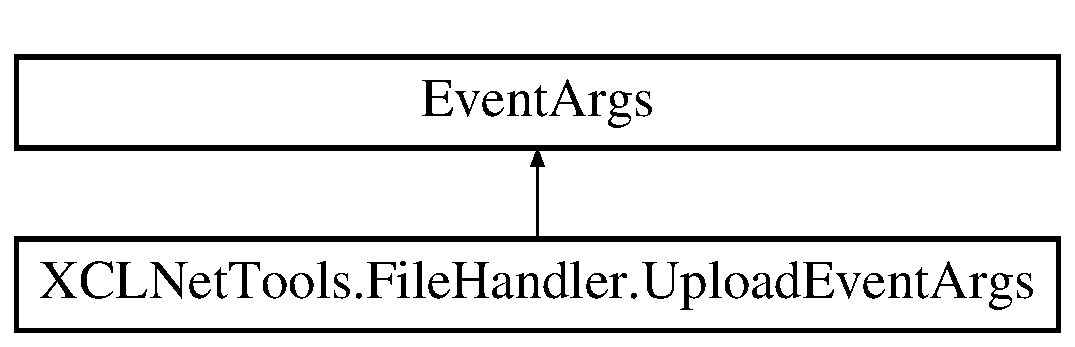
\includegraphics[height=2.000000cm]{class_x_c_l_net_tools_1_1_file_handler_1_1_upload_event_args}
\end{center}
\end{figure}
\subsection*{属性}
\begin{DoxyCompactItemize}
\item 
int \hyperlink{class_x_c_l_net_tools_1_1_file_handler_1_1_upload_event_args_aeb753c87413d86d610121060635794e1}{Bytes\+Sent}\hspace{0.3cm}{\ttfamily  \mbox{[}get, set\mbox{]}}
\begin{DoxyCompactList}\small\item\em 已发送的字节数 \end{DoxyCompactList}\item 
int \hyperlink{class_x_c_l_net_tools_1_1_file_handler_1_1_upload_event_args_a874a8bc16016a3d11eb9aa52f9670eb4}{Total\+Bytes}\hspace{0.3cm}{\ttfamily  \mbox{[}get, set\mbox{]}}
\begin{DoxyCompactList}\small\item\em 总字节数 \end{DoxyCompactList}\end{DoxyCompactItemize}


\subsection{详细描述}
上传数据参数 



在文件 Http\+Proc.\+cs 第 23 行定义.



\subsection{属性说明}
\mbox{\Hypertarget{class_x_c_l_net_tools_1_1_file_handler_1_1_upload_event_args_aeb753c87413d86d610121060635794e1}\label{class_x_c_l_net_tools_1_1_file_handler_1_1_upload_event_args_aeb753c87413d86d610121060635794e1}} 
\index{X\+C\+L\+Net\+Tools\+::\+File\+Handler\+::\+Upload\+Event\+Args@{X\+C\+L\+Net\+Tools\+::\+File\+Handler\+::\+Upload\+Event\+Args}!Bytes\+Sent@{Bytes\+Sent}}
\index{Bytes\+Sent@{Bytes\+Sent}!X\+C\+L\+Net\+Tools\+::\+File\+Handler\+::\+Upload\+Event\+Args@{X\+C\+L\+Net\+Tools\+::\+File\+Handler\+::\+Upload\+Event\+Args}}
\subsubsection{\texorpdfstring{Bytes\+Sent}{BytesSent}}
{\footnotesize\ttfamily int X\+C\+L\+Net\+Tools.\+File\+Handler.\+Upload\+Event\+Args.\+Bytes\+Sent\hspace{0.3cm}{\ttfamily [get]}, {\ttfamily [set]}}



已发送的字节数 



在文件 Http\+Proc.\+cs 第 28 行定义.

\mbox{\Hypertarget{class_x_c_l_net_tools_1_1_file_handler_1_1_upload_event_args_a874a8bc16016a3d11eb9aa52f9670eb4}\label{class_x_c_l_net_tools_1_1_file_handler_1_1_upload_event_args_a874a8bc16016a3d11eb9aa52f9670eb4}} 
\index{X\+C\+L\+Net\+Tools\+::\+File\+Handler\+::\+Upload\+Event\+Args@{X\+C\+L\+Net\+Tools\+::\+File\+Handler\+::\+Upload\+Event\+Args}!Total\+Bytes@{Total\+Bytes}}
\index{Total\+Bytes@{Total\+Bytes}!X\+C\+L\+Net\+Tools\+::\+File\+Handler\+::\+Upload\+Event\+Args@{X\+C\+L\+Net\+Tools\+::\+File\+Handler\+::\+Upload\+Event\+Args}}
\subsubsection{\texorpdfstring{Total\+Bytes}{TotalBytes}}
{\footnotesize\ttfamily int X\+C\+L\+Net\+Tools.\+File\+Handler.\+Upload\+Event\+Args.\+Total\+Bytes\hspace{0.3cm}{\ttfamily [get]}, {\ttfamily [set]}}



总字节数 



在文件 Http\+Proc.\+cs 第 33 行定义.



该类的文档由以下文件生成\+:\begin{DoxyCompactItemize}
\item 
D\+:/\+My\+Data/\+Git\+Hub/\+X\+C\+L\+Net\+Tools/\+X\+C\+L\+Net\+Tools/\+File\+Handler/\hyperlink{_http_proc_8cs}{Http\+Proc.\+cs}\end{DoxyCompactItemize}

\hypertarget{class_x_c_l_net_tools_1_1_string_hander_1_1_url_oper}{\section{X\-C\-L\-Net\-Tools.\-String\-Hander.\-Url\-Oper类 参考}
\label{class_x_c_l_net_tools_1_1_string_hander_1_1_url_oper}\index{X\-C\-L\-Net\-Tools.\-String\-Hander.\-Url\-Oper@{X\-C\-L\-Net\-Tools.\-String\-Hander.\-Url\-Oper}}
}


U\-R\-L的操作类  


\subsection*{静态 Public 成员函数}
\begin{DoxyCompactItemize}
\item 
static string \hyperlink{class_x_c_l_net_tools_1_1_string_hander_1_1_url_oper_a63e4554d226a4e22cdf68614d6fdd1c1}{Add\-Param} (string url, string name, string value)
\begin{DoxyCompactList}\small\item\em 添加\-U\-R\-L参数 \end{DoxyCompactList}\item 
static string \hyperlink{class_x_c_l_net_tools_1_1_string_hander_1_1_url_oper_ae4e0043d5ebfc5401f90242992071fdc}{Add\-Param} (string url, Name\-Value\-Collection param)
\begin{DoxyCompactList}\small\item\em 添加\-U\-R\-L参数 \end{DoxyCompactList}\item 
static string \hyperlink{class_x_c_l_net_tools_1_1_string_hander_1_1_url_oper_adda296014d4edff564f69975de4d3171}{Update\-Param} (string url, string param\-Name, string value)
\begin{DoxyCompactList}\small\item\em 更新\-U\-R\-L参数 \end{DoxyCompactList}\item 
static string \hyperlink{class_x_c_l_net_tools_1_1_string_hander_1_1_url_oper_aee0fcf87276a12d12e71d2d905e286e0}{Remove\-Param} (string url, string param\-Name)
\begin{DoxyCompactList}\small\item\em 删除url参数 \end{DoxyCompactList}\item 
static void \hyperlink{class_x_c_l_net_tools_1_1_string_hander_1_1_url_oper_a8786e6cf26b3496627bbcc037ca72ca7}{Parse\-Url} (string url, out string base\-Url, out Name\-Value\-Collection nvc)
\begin{DoxyCompactList}\small\item\em 分析 url 字符串中的参数信息 \end{DoxyCompactList}\item 
static int \hyperlink{class_x_c_l_net_tools_1_1_string_hander_1_1_url_oper_ac5c640bfc662741345164efa1efbc525}{Get\-Url\-Error} (string curl)
\begin{DoxyCompactList}\small\item\em 获取指定\-U\-R\-L的请求状态: 200 -\/ 确定。客户端请求已成功。 201 -\/ 已创建。 202 -\/ 已接受。 400 -\/ 错误的请求 401 -\/ 访问被拒绝 403 -\/ 禁止访问 404 -\/ 未找到 405 -\/ 用来访问本页面的 H\-T\-T\-P 谓词不被允许(方法不被允许) 406 -\/ 客户端浏览器不接受所请求页面的 M\-I\-M\-E 类型。 407 -\/ 要求进行代理身份验证。 412 -\/ 前提条件失败。 413 – 请求实体太大。 414 -\/ 请求 U\-R\-I 太长。 415 – 不支持的媒体类型。 416 – 所请求的范围无法满足。 417 – 执行失败。 423 – 锁定的错误 500 -\/ 内部服务器错误。 501 -\/ 页眉值指定了未实现的配置。 502 -\/ Web 服务器用作网关或代理服务器时收到了无效响应。 503 -\/ 服务不可用。这个错误代码为 I\-I\-S 6.\-0 所专用。 504 -\/ 网关超时。 505 -\/ H\-T\-T\-P 版本不受支持。 /summary$>$ param name=\char`\"{}curl\char`\"{}$>$要请求的\-U\-R\-L

returns$>$状态码\end{DoxyCompactList}\end{DoxyCompactItemize}


\subsection{详细描述}
U\-R\-L的操作类 



在文件 Url\-Oper.\-cs 第 21 行定义.



\subsection{成员函数说明}
\hypertarget{class_x_c_l_net_tools_1_1_string_hander_1_1_url_oper_a63e4554d226a4e22cdf68614d6fdd1c1}{\index{X\-C\-L\-Net\-Tools\-::\-String\-Hander\-::\-Url\-Oper@{X\-C\-L\-Net\-Tools\-::\-String\-Hander\-::\-Url\-Oper}!Add\-Param@{Add\-Param}}
\index{Add\-Param@{Add\-Param}!XCLNetTools::StringHander::UrlOper@{X\-C\-L\-Net\-Tools\-::\-String\-Hander\-::\-Url\-Oper}}
\subsubsection[{Add\-Param}]{\setlength{\rightskip}{0pt plus 5cm}static string X\-C\-L\-Net\-Tools.\-String\-Hander.\-Url\-Oper.\-Add\-Param (
\begin{DoxyParamCaption}
\item[{string}]{url, }
\item[{string}]{name, }
\item[{string}]{value}
\end{DoxyParamCaption}
)\hspace{0.3cm}{\ttfamily [static]}}}\label{class_x_c_l_net_tools_1_1_string_hander_1_1_url_oper_a63e4554d226a4e22cdf68614d6fdd1c1}


添加\-U\-R\-L参数 


\begin{DoxyParams}{参数}
{\em url} & url\\
\hline
{\em name} & 参数名\\
\hline
{\em value} & 参数值\\
\hline
\end{DoxyParams}
\begin{DoxyReturn}{返回}
新的url
\end{DoxyReturn}


在文件 Url\-Oper.\-cs 第 32 行定义.

\hypertarget{class_x_c_l_net_tools_1_1_string_hander_1_1_url_oper_ae4e0043d5ebfc5401f90242992071fdc}{\index{X\-C\-L\-Net\-Tools\-::\-String\-Hander\-::\-Url\-Oper@{X\-C\-L\-Net\-Tools\-::\-String\-Hander\-::\-Url\-Oper}!Add\-Param@{Add\-Param}}
\index{Add\-Param@{Add\-Param}!XCLNetTools::StringHander::UrlOper@{X\-C\-L\-Net\-Tools\-::\-String\-Hander\-::\-Url\-Oper}}
\subsubsection[{Add\-Param}]{\setlength{\rightskip}{0pt plus 5cm}static string X\-C\-L\-Net\-Tools.\-String\-Hander.\-Url\-Oper.\-Add\-Param (
\begin{DoxyParamCaption}
\item[{string}]{url, }
\item[{Name\-Value\-Collection}]{param}
\end{DoxyParamCaption}
)\hspace{0.3cm}{\ttfamily [static]}}}\label{class_x_c_l_net_tools_1_1_string_hander_1_1_url_oper_ae4e0043d5ebfc5401f90242992071fdc}


添加\-U\-R\-L参数 


\begin{DoxyParams}{参数}
{\em url} & url\\
\hline
{\em param} & 参数集合\\
\hline
\end{DoxyParams}
\begin{DoxyReturn}{返回}
新的url
\end{DoxyReturn}


在文件 Url\-Oper.\-cs 第 45 行定义.

\hypertarget{class_x_c_l_net_tools_1_1_string_hander_1_1_url_oper_ac5c640bfc662741345164efa1efbc525}{\index{X\-C\-L\-Net\-Tools\-::\-String\-Hander\-::\-Url\-Oper@{X\-C\-L\-Net\-Tools\-::\-String\-Hander\-::\-Url\-Oper}!Get\-Url\-Error@{Get\-Url\-Error}}
\index{Get\-Url\-Error@{Get\-Url\-Error}!XCLNetTools::StringHander::UrlOper@{X\-C\-L\-Net\-Tools\-::\-String\-Hander\-::\-Url\-Oper}}
\subsubsection[{Get\-Url\-Error}]{\setlength{\rightskip}{0pt plus 5cm}static int X\-C\-L\-Net\-Tools.\-String\-Hander.\-Url\-Oper.\-Get\-Url\-Error (
\begin{DoxyParamCaption}
\item[{string}]{curl}
\end{DoxyParamCaption}
)\hspace{0.3cm}{\ttfamily [static]}}}\label{class_x_c_l_net_tools_1_1_string_hander_1_1_url_oper_ac5c640bfc662741345164efa1efbc525}


获取指定\-U\-R\-L的请求状态: 200 -\/ 确定。客户端请求已成功。 201 -\/ 已创建。 202 -\/ 已接受。 400 -\/ 错误的请求 401 -\/ 访问被拒绝 403 -\/ 禁止访问 404 -\/ 未找到 405 -\/ 用来访问本页面的 H\-T\-T\-P 谓词不被允许(方法不被允许) 406 -\/ 客户端浏览器不接受所请求页面的 M\-I\-M\-E 类型。 407 -\/ 要求进行代理身份验证。 412 -\/ 前提条件失败。 413 – 请求实体太大。 414 -\/ 请求 U\-R\-I 太长。 415 – 不支持的媒体类型。 416 – 所请求的范围无法满足。 417 – 执行失败。 423 – 锁定的错误 500 -\/ 内部服务器错误。 501 -\/ 页眉值指定了未实现的配置。 502 -\/ Web 服务器用作网关或代理服务器时收到了无效响应。 503 -\/ 服务不可用。这个错误代码为 I\-I\-S 6.\-0 所专用。 504 -\/ 网关超时。 505 -\/ H\-T\-T\-P 版本不受支持。 /summary$>$ param name=\char`\"{}curl\char`\"{}$>$要请求的\-U\-R\-L

returns$>$状态码



在文件 Url\-Oper.\-cs 第 222 行定义.

\hypertarget{class_x_c_l_net_tools_1_1_string_hander_1_1_url_oper_a8786e6cf26b3496627bbcc037ca72ca7}{\index{X\-C\-L\-Net\-Tools\-::\-String\-Hander\-::\-Url\-Oper@{X\-C\-L\-Net\-Tools\-::\-String\-Hander\-::\-Url\-Oper}!Parse\-Url@{Parse\-Url}}
\index{Parse\-Url@{Parse\-Url}!XCLNetTools::StringHander::UrlOper@{X\-C\-L\-Net\-Tools\-::\-String\-Hander\-::\-Url\-Oper}}
\subsubsection[{Parse\-Url}]{\setlength{\rightskip}{0pt plus 5cm}static void X\-C\-L\-Net\-Tools.\-String\-Hander.\-Url\-Oper.\-Parse\-Url (
\begin{DoxyParamCaption}
\item[{string}]{url, }
\item[{out string}]{base\-Url, }
\item[{out Name\-Value\-Collection}]{nvc}
\end{DoxyParamCaption}
)\hspace{0.3cm}{\ttfamily [static]}}}\label{class_x_c_l_net_tools_1_1_string_hander_1_1_url_oper_a8786e6cf26b3496627bbcc037ca72ca7}


分析 url 字符串中的参数信息 


\begin{DoxyParams}{参数}
{\em url} & 输入的 U\-R\-L\\
\hline
{\em base\-Url} & 输出 U\-R\-L 的基础部分\\
\hline
{\em nvc} & 输出分析后得到的 (参数名,参数值) 的集合\\
\hline
\end{DoxyParams}


在文件 Url\-Oper.\-cs 第 159 行定义.

\hypertarget{class_x_c_l_net_tools_1_1_string_hander_1_1_url_oper_aee0fcf87276a12d12e71d2d905e286e0}{\index{X\-C\-L\-Net\-Tools\-::\-String\-Hander\-::\-Url\-Oper@{X\-C\-L\-Net\-Tools\-::\-String\-Hander\-::\-Url\-Oper}!Remove\-Param@{Remove\-Param}}
\index{Remove\-Param@{Remove\-Param}!XCLNetTools::StringHander::UrlOper@{X\-C\-L\-Net\-Tools\-::\-String\-Hander\-::\-Url\-Oper}}
\subsubsection[{Remove\-Param}]{\setlength{\rightskip}{0pt plus 5cm}static string X\-C\-L\-Net\-Tools.\-String\-Hander.\-Url\-Oper.\-Remove\-Param (
\begin{DoxyParamCaption}
\item[{string}]{url, }
\item[{string}]{param\-Name}
\end{DoxyParamCaption}
)\hspace{0.3cm}{\ttfamily [static]}}}\label{class_x_c_l_net_tools_1_1_string_hander_1_1_url_oper_aee0fcf87276a12d12e71d2d905e286e0}


删除url参数 


\begin{DoxyParams}{参数}
{\em url} & url\\
\hline
{\em param\-Name} & 参数名\\
\hline
\end{DoxyParams}
\begin{DoxyReturn}{返回}
新的url
\end{DoxyReturn}


在文件 Url\-Oper.\-cs 第 110 行定义.

\hypertarget{class_x_c_l_net_tools_1_1_string_hander_1_1_url_oper_adda296014d4edff564f69975de4d3171}{\index{X\-C\-L\-Net\-Tools\-::\-String\-Hander\-::\-Url\-Oper@{X\-C\-L\-Net\-Tools\-::\-String\-Hander\-::\-Url\-Oper}!Update\-Param@{Update\-Param}}
\index{Update\-Param@{Update\-Param}!XCLNetTools::StringHander::UrlOper@{X\-C\-L\-Net\-Tools\-::\-String\-Hander\-::\-Url\-Oper}}
\subsubsection[{Update\-Param}]{\setlength{\rightskip}{0pt plus 5cm}static string X\-C\-L\-Net\-Tools.\-String\-Hander.\-Url\-Oper.\-Update\-Param (
\begin{DoxyParamCaption}
\item[{string}]{url, }
\item[{string}]{param\-Name, }
\item[{string}]{value}
\end{DoxyParamCaption}
)\hspace{0.3cm}{\ttfamily [static]}}}\label{class_x_c_l_net_tools_1_1_string_hander_1_1_url_oper_adda296014d4edff564f69975de4d3171}


更新\-U\-R\-L参数 


\begin{DoxyParams}{参数}
{\em url} & url\\
\hline
{\em param\-Name} & 参数名\\
\hline
{\em value} & 参数值\\
\hline
\end{DoxyParams}
\begin{DoxyReturn}{返回}
新的url
\end{DoxyReturn}


在文件 Url\-Oper.\-cs 第 88 行定义.



该类的文档由以下文件生成\-:\begin{DoxyCompactItemize}
\item 
D\-:/\-My\-Data/\-My\-Git/\-Git\-Hub/\-X\-C\-L\-Net\-Tools/\-X\-C\-L\-Net\-Tools/\-String\-Hander/\hyperlink{_url_oper_8cs}{Url\-Oper.\-cs}\end{DoxyCompactItemize}

\hypertarget{class_x_c_l_net_tools_1_1_file_handler_1_1_verification_code}{}\section{X\+C\+L\+Net\+Tools.\+File\+Handler.\+Verification\+Code类 参考}
\label{class_x_c_l_net_tools_1_1_file_handler_1_1_verification_code}\index{X\+C\+L\+Net\+Tools.\+File\+Handler.\+Verification\+Code@{X\+C\+L\+Net\+Tools.\+File\+Handler.\+Verification\+Code}}


验证码相关  


\subsection*{静态 Public 成员函数}
\begin{DoxyCompactItemize}
\item 
static string \hyperlink{class_x_c_l_net_tools_1_1_file_handler_1_1_verification_code_af4beced22b07b395e6ae37452a895f32}{Generate\+Check\+Code} ()
\begin{DoxyCompactList}\small\item\em 生成验证码的随机数 \end{DoxyCompactList}\item 
static void \hyperlink{class_x_c_l_net_tools_1_1_file_handler_1_1_verification_code_acde0d83935e0d55da7a29725026a72e9}{Create\+Check\+Code\+Image} (string check\+Code)
\begin{DoxyCompactList}\small\item\em 生成验证码图片 \end{DoxyCompactList}\end{DoxyCompactItemize}


\subsection{详细描述}
验证码相关 



在文件 Verification\+Code.\+cs 第 18 行定义.



\subsection{成员函数说明}
\index{X\+C\+L\+Net\+Tools\+::\+File\+Handler\+::\+Verification\+Code@{X\+C\+L\+Net\+Tools\+::\+File\+Handler\+::\+Verification\+Code}!Create\+Check\+Code\+Image@{Create\+Check\+Code\+Image}}
\index{Create\+Check\+Code\+Image@{Create\+Check\+Code\+Image}!X\+C\+L\+Net\+Tools\+::\+File\+Handler\+::\+Verification\+Code@{X\+C\+L\+Net\+Tools\+::\+File\+Handler\+::\+Verification\+Code}}
\subsubsection[{\texorpdfstring{Create\+Check\+Code\+Image(string check\+Code)}{CreateCheckCodeImage(string checkCode)}}]{\setlength{\rightskip}{0pt plus 5cm}static void X\+C\+L\+Net\+Tools.\+File\+Handler.\+Verification\+Code.\+Create\+Check\+Code\+Image (
\begin{DoxyParamCaption}
\item[{string}]{check\+Code}
\end{DoxyParamCaption}
)\hspace{0.3cm}{\ttfamily [static]}}\hypertarget{class_x_c_l_net_tools_1_1_file_handler_1_1_verification_code_acde0d83935e0d55da7a29725026a72e9}{}\label{class_x_c_l_net_tools_1_1_file_handler_1_1_verification_code_acde0d83935e0d55da7a29725026a72e9}


生成验证码图片 


\begin{DoxyParams}{参数}
{\em check\+Code} & 字符代码\\
\hline
\end{DoxyParams}


在文件 Verification\+Code.\+cs 第 46 行定义.

\index{X\+C\+L\+Net\+Tools\+::\+File\+Handler\+::\+Verification\+Code@{X\+C\+L\+Net\+Tools\+::\+File\+Handler\+::\+Verification\+Code}!Generate\+Check\+Code@{Generate\+Check\+Code}}
\index{Generate\+Check\+Code@{Generate\+Check\+Code}!X\+C\+L\+Net\+Tools\+::\+File\+Handler\+::\+Verification\+Code@{X\+C\+L\+Net\+Tools\+::\+File\+Handler\+::\+Verification\+Code}}
\subsubsection[{\texorpdfstring{Generate\+Check\+Code()}{GenerateCheckCode()}}]{\setlength{\rightskip}{0pt plus 5cm}static string X\+C\+L\+Net\+Tools.\+File\+Handler.\+Verification\+Code.\+Generate\+Check\+Code (
\begin{DoxyParamCaption}
{}
\end{DoxyParamCaption}
)\hspace{0.3cm}{\ttfamily [static]}}\hypertarget{class_x_c_l_net_tools_1_1_file_handler_1_1_verification_code_af4beced22b07b395e6ae37452a895f32}{}\label{class_x_c_l_net_tools_1_1_file_handler_1_1_verification_code_af4beced22b07b395e6ae37452a895f32}


生成验证码的随机数 

\begin{DoxyReturn}{返回}
随机数
\end{DoxyReturn}


在文件 Verification\+Code.\+cs 第 24 行定义.



该类的文档由以下文件生成\+:\begin{DoxyCompactItemize}
\item 
E\+:/\+Git\+Hub/\+X\+C\+L\+Net\+Tools/\+X\+C\+L\+Net\+Tools/\+File\+Handler/\hyperlink{_verification_code_8cs}{Verification\+Code.\+cs}\end{DoxyCompactItemize}

\hypertarget{class_x_c_l_net_tools_1_1_file_handler_1_1_web_client}{}\section{X\+C\+L\+Net\+Tools.\+File\+Handler.\+Web\+Client类 参考}
\label{class_x_c_l_net_tools_1_1_file_handler_1_1_web_client}\index{X\+C\+L\+Net\+Tools.\+File\+Handler.\+Web\+Client@{X\+C\+L\+Net\+Tools.\+File\+Handler.\+Web\+Client}}


\hyperlink{class_x_c_l_net_tools_1_1_file_handler_1_1_web_client}{Web\+Client}  


\subsection*{Public 成员函数}
\begin{DoxyCompactItemize}
\item 
\hyperlink{class_x_c_l_net_tools_1_1_file_handler_1_1_web_client_a8f3cbaf1baf5d142caab2f6c9cc04a7f}{Web\+Client} ()
\begin{DoxyCompactList}\small\item\em 创建\+Web\+Client的实例 \end{DoxyCompactList}\item 
string \hyperlink{class_x_c_l_net_tools_1_1_file_handler_1_1_web_client_a504910f5e28a6fa620853f069d3c756b}{Get\+Html} (string url)
\begin{DoxyCompactList}\small\item\em 获取网页源代码 \end{DoxyCompactList}\item 
void \hyperlink{class_x_c_l_net_tools_1_1_file_handler_1_1_web_client_ace80aaf94d3e0c6eceb3ad182b8de947}{Download\+File} (string url, string filename)
\begin{DoxyCompactList}\small\item\em 下载文件 \end{DoxyCompactList}\item 
byte \mbox{[}$\,$\mbox{]} \hyperlink{class_x_c_l_net_tools_1_1_file_handler_1_1_web_client_a7208770077f210c3dd7bee2b34f0a4eb}{Get\+Data} (string url)
\begin{DoxyCompactList}\small\item\em 从指定\+U\+R\+L下载数据 \end{DoxyCompactList}\item 
string \hyperlink{class_x_c_l_net_tools_1_1_file_handler_1_1_web_client_ab2497ff9ed5a5b867362b7bc0b38edb1}{Post} (string url, string post\+Data)
\begin{DoxyCompactList}\small\item\em 向指定\+U\+R\+L发送文本数据 \end{DoxyCompactList}\item 
string \hyperlink{class_x_c_l_net_tools_1_1_file_handler_1_1_web_client_ad799cba2f787fba4c0ca4fc6e86ee831}{Post} (string url, byte\mbox{[}$\,$\mbox{]} post\+Data)
\begin{DoxyCompactList}\small\item\em 向指定\+U\+R\+L发送字节数据 \end{DoxyCompactList}\item 
string \hyperlink{class_x_c_l_net_tools_1_1_file_handler_1_1_web_client_ab1556a7a601a8425c7d6bcecb09d6cf2}{Post} (string url, \hyperlink{class_x_c_l_net_tools_1_1_file_handler_1_1_multipart_form}{Multipart\+Form} mulitpart\+Form)
\begin{DoxyCompactList}\small\item\em 向指定网址发送mulitpart编码的数据 \end{DoxyCompactList}\end{DoxyCompactItemize}
\subsection*{属性}
\begin{DoxyCompactItemize}
\item 
int \hyperlink{class_x_c_l_net_tools_1_1_file_handler_1_1_web_client_a192f27c95b8274758ca9d68c620de7c3}{Buffer\+Size}\hspace{0.3cm}{\ttfamily  \mbox{[}get, set\mbox{]}}
\begin{DoxyCompactList}\small\item\em 设置发送和接收的数据缓冲大小 \end{DoxyCompactList}\item 
Web\+Header\+Collection \hyperlink{class_x_c_l_net_tools_1_1_file_handler_1_1_web_client_a3d00d3457c23ce30274af963f4cab6bb}{Response\+Headers}\hspace{0.3cm}{\ttfamily  \mbox{[}get\mbox{]}}
\begin{DoxyCompactList}\small\item\em 获取响应头集合 \end{DoxyCompactList}\item 
Web\+Header\+Collection \hyperlink{class_x_c_l_net_tools_1_1_file_handler_1_1_web_client_a89d4bf2af70a2a0991904b1b61c8dd1d}{Request\+Headers}\hspace{0.3cm}{\ttfamily  \mbox{[}get\mbox{]}}
\begin{DoxyCompactList}\small\item\em 获取请求头集合 \end{DoxyCompactList}\item 
Web\+Proxy \hyperlink{class_x_c_l_net_tools_1_1_file_handler_1_1_web_client_ac2f17eefdc2372eb01a6be915d19c0ba}{Proxy}\hspace{0.3cm}{\ttfamily  \mbox{[}get, set\mbox{]}}
\begin{DoxyCompactList}\small\item\em 获取或设置代理 \end{DoxyCompactList}\item 
Encoding \hyperlink{class_x_c_l_net_tools_1_1_file_handler_1_1_web_client_a9bd02ab7f0198d34a44487c5d8c02f19}{Encoding}\hspace{0.3cm}{\ttfamily  \mbox{[}get, set\mbox{]}}
\begin{DoxyCompactList}\small\item\em 获取或设置请求与响应的文本编码方式 \end{DoxyCompactList}\item 
string \hyperlink{class_x_c_l_net_tools_1_1_file_handler_1_1_web_client_a67e90e96bd067171c16cb84d75f66c3a}{Resp\+Html}\hspace{0.3cm}{\ttfamily  \mbox{[}get, set\mbox{]}}
\begin{DoxyCompactList}\small\item\em 获取或设置响应的html代码 \end{DoxyCompactList}\item 
Cookie\+Container \hyperlink{class_x_c_l_net_tools_1_1_file_handler_1_1_web_client_adeaa1201074e43df3743d76ea77cf06e}{Cookie\+Container}\hspace{0.3cm}{\ttfamily  \mbox{[}get, set\mbox{]}}
\begin{DoxyCompactList}\small\item\em 获取或设置与请求关联的\+Cookie容器 \end{DoxyCompactList}\end{DoxyCompactItemize}
\subsection*{事件}
\begin{DoxyCompactItemize}
\item 
Event\+Handler$<$ \hyperlink{class_x_c_l_net_tools_1_1_file_handler_1_1_upload_event_args}{Upload\+Event\+Args} $>$ \hyperlink{class_x_c_l_net_tools_1_1_file_handler_1_1_web_client_abe950fa329508b4c52e3181aeb97585f}{Upload\+Progress\+Changed}
\begin{DoxyCompactList}\small\item\em 上传事件 \end{DoxyCompactList}\item 
Event\+Handler$<$ \hyperlink{class_x_c_l_net_tools_1_1_file_handler_1_1_download_event_args}{Download\+Event\+Args} $>$ \hyperlink{class_x_c_l_net_tools_1_1_file_handler_1_1_web_client_aa1e50d608381b728356547eff9f80213}{Download\+Progress\+Changed}
\begin{DoxyCompactList}\small\item\em 下载事件 \end{DoxyCompactList}\end{DoxyCompactItemize}


\subsection{详细描述}
\hyperlink{class_x_c_l_net_tools_1_1_file_handler_1_1_web_client}{Web\+Client} 



在文件 Http\+Proc.\+cs 第 87 行定义.



\subsection{构造及析构函数说明}
\mbox{\Hypertarget{class_x_c_l_net_tools_1_1_file_handler_1_1_web_client_a8f3cbaf1baf5d142caab2f6c9cc04a7f}\label{class_x_c_l_net_tools_1_1_file_handler_1_1_web_client_a8f3cbaf1baf5d142caab2f6c9cc04a7f}} 
\index{X\+C\+L\+Net\+Tools\+::\+File\+Handler\+::\+Web\+Client@{X\+C\+L\+Net\+Tools\+::\+File\+Handler\+::\+Web\+Client}!Web\+Client@{Web\+Client}}
\index{Web\+Client@{Web\+Client}!X\+C\+L\+Net\+Tools\+::\+File\+Handler\+::\+Web\+Client@{X\+C\+L\+Net\+Tools\+::\+File\+Handler\+::\+Web\+Client}}
\subsubsection{\texorpdfstring{Web\+Client()}{WebClient()}}
{\footnotesize\ttfamily X\+C\+L\+Net\+Tools.\+File\+Handler.\+Web\+Client.\+Web\+Client (\begin{DoxyParamCaption}{ }\end{DoxyParamCaption})}



创建\+Web\+Client的实例 



在文件 Http\+Proc.\+cs 第 115 行定义.



\subsection{成员函数说明}
\mbox{\Hypertarget{class_x_c_l_net_tools_1_1_file_handler_1_1_web_client_ace80aaf94d3e0c6eceb3ad182b8de947}\label{class_x_c_l_net_tools_1_1_file_handler_1_1_web_client_ace80aaf94d3e0c6eceb3ad182b8de947}} 
\index{X\+C\+L\+Net\+Tools\+::\+File\+Handler\+::\+Web\+Client@{X\+C\+L\+Net\+Tools\+::\+File\+Handler\+::\+Web\+Client}!Download\+File@{Download\+File}}
\index{Download\+File@{Download\+File}!X\+C\+L\+Net\+Tools\+::\+File\+Handler\+::\+Web\+Client@{X\+C\+L\+Net\+Tools\+::\+File\+Handler\+::\+Web\+Client}}
\subsubsection{\texorpdfstring{Download\+File()}{DownloadFile()}}
{\footnotesize\ttfamily void X\+C\+L\+Net\+Tools.\+File\+Handler.\+Web\+Client.\+Download\+File (\begin{DoxyParamCaption}\item[{string}]{url,  }\item[{string}]{filename }\end{DoxyParamCaption})}



下载文件 


\begin{DoxyParams}{参数}
{\em url} & 文件\+U\+R\+L地址\\
\hline
{\em filename} & 文件保存完整路径\\
\hline
\end{DoxyParams}


在文件 Http\+Proc.\+cs 第 199 行定义.

\mbox{\Hypertarget{class_x_c_l_net_tools_1_1_file_handler_1_1_web_client_a7208770077f210c3dd7bee2b34f0a4eb}\label{class_x_c_l_net_tools_1_1_file_handler_1_1_web_client_a7208770077f210c3dd7bee2b34f0a4eb}} 
\index{X\+C\+L\+Net\+Tools\+::\+File\+Handler\+::\+Web\+Client@{X\+C\+L\+Net\+Tools\+::\+File\+Handler\+::\+Web\+Client}!Get\+Data@{Get\+Data}}
\index{Get\+Data@{Get\+Data}!X\+C\+L\+Net\+Tools\+::\+File\+Handler\+::\+Web\+Client@{X\+C\+L\+Net\+Tools\+::\+File\+Handler\+::\+Web\+Client}}
\subsubsection{\texorpdfstring{Get\+Data()}{GetData()}}
{\footnotesize\ttfamily byte \mbox{[}$\,$\mbox{]} X\+C\+L\+Net\+Tools.\+File\+Handler.\+Web\+Client.\+Get\+Data (\begin{DoxyParamCaption}\item[{string}]{url }\end{DoxyParamCaption})}



从指定\+U\+R\+L下载数据 


\begin{DoxyParams}{参数}
{\em url} & 网址\\
\hline
\end{DoxyParams}
\begin{DoxyReturn}{返回}

\end{DoxyReturn}


在文件 Http\+Proc.\+cs 第 220 行定义.

\mbox{\Hypertarget{class_x_c_l_net_tools_1_1_file_handler_1_1_web_client_a504910f5e28a6fa620853f069d3c756b}\label{class_x_c_l_net_tools_1_1_file_handler_1_1_web_client_a504910f5e28a6fa620853f069d3c756b}} 
\index{X\+C\+L\+Net\+Tools\+::\+File\+Handler\+::\+Web\+Client@{X\+C\+L\+Net\+Tools\+::\+File\+Handler\+::\+Web\+Client}!Get\+Html@{Get\+Html}}
\index{Get\+Html@{Get\+Html}!X\+C\+L\+Net\+Tools\+::\+File\+Handler\+::\+Web\+Client@{X\+C\+L\+Net\+Tools\+::\+File\+Handler\+::\+Web\+Client}}
\subsubsection{\texorpdfstring{Get\+Html()}{GetHtml()}}
{\footnotesize\ttfamily string X\+C\+L\+Net\+Tools.\+File\+Handler.\+Web\+Client.\+Get\+Html (\begin{DoxyParamCaption}\item[{string}]{url }\end{DoxyParamCaption})}



获取网页源代码 


\begin{DoxyParams}{参数}
{\em url} & 网址\\
\hline
\end{DoxyParams}
\begin{DoxyReturn}{返回}

\end{DoxyReturn}


在文件 Http\+Proc.\+cs 第 187 行定义.

\mbox{\Hypertarget{class_x_c_l_net_tools_1_1_file_handler_1_1_web_client_ab2497ff9ed5a5b867362b7bc0b38edb1}\label{class_x_c_l_net_tools_1_1_file_handler_1_1_web_client_ab2497ff9ed5a5b867362b7bc0b38edb1}} 
\index{X\+C\+L\+Net\+Tools\+::\+File\+Handler\+::\+Web\+Client@{X\+C\+L\+Net\+Tools\+::\+File\+Handler\+::\+Web\+Client}!Post@{Post}}
\index{Post@{Post}!X\+C\+L\+Net\+Tools\+::\+File\+Handler\+::\+Web\+Client@{X\+C\+L\+Net\+Tools\+::\+File\+Handler\+::\+Web\+Client}}
\subsubsection{\texorpdfstring{Post()}{Post()}\hspace{0.1cm}{\footnotesize\ttfamily [1/3]}}
{\footnotesize\ttfamily string X\+C\+L\+Net\+Tools.\+File\+Handler.\+Web\+Client.\+Post (\begin{DoxyParamCaption}\item[{string}]{url,  }\item[{string}]{post\+Data }\end{DoxyParamCaption})}



向指定\+U\+R\+L发送文本数据 


\begin{DoxyParams}{参数}
{\em url} & 网址\\
\hline
{\em post\+Data} & urlencode编码的文本数据\\
\hline
\end{DoxyParams}
\begin{DoxyReturn}{返回}

\end{DoxyReturn}


在文件 Http\+Proc.\+cs 第 232 行定义.

\mbox{\Hypertarget{class_x_c_l_net_tools_1_1_file_handler_1_1_web_client_ad799cba2f787fba4c0ca4fc6e86ee831}\label{class_x_c_l_net_tools_1_1_file_handler_1_1_web_client_ad799cba2f787fba4c0ca4fc6e86ee831}} 
\index{X\+C\+L\+Net\+Tools\+::\+File\+Handler\+::\+Web\+Client@{X\+C\+L\+Net\+Tools\+::\+File\+Handler\+::\+Web\+Client}!Post@{Post}}
\index{Post@{Post}!X\+C\+L\+Net\+Tools\+::\+File\+Handler\+::\+Web\+Client@{X\+C\+L\+Net\+Tools\+::\+File\+Handler\+::\+Web\+Client}}
\subsubsection{\texorpdfstring{Post()}{Post()}\hspace{0.1cm}{\footnotesize\ttfamily [2/3]}}
{\footnotesize\ttfamily string X\+C\+L\+Net\+Tools.\+File\+Handler.\+Web\+Client.\+Post (\begin{DoxyParamCaption}\item[{string}]{url,  }\item[{byte \mbox{[}$\,$\mbox{]}}]{post\+Data }\end{DoxyParamCaption})}



向指定\+U\+R\+L发送字节数据 


\begin{DoxyParams}{参数}
{\em url} & 网址\\
\hline
{\em post\+Data} & 发送的字节数组\\
\hline
\end{DoxyParams}
\begin{DoxyReturn}{返回}

\end{DoxyReturn}


在文件 Http\+Proc.\+cs 第 244 行定义.

\mbox{\Hypertarget{class_x_c_l_net_tools_1_1_file_handler_1_1_web_client_ab1556a7a601a8425c7d6bcecb09d6cf2}\label{class_x_c_l_net_tools_1_1_file_handler_1_1_web_client_ab1556a7a601a8425c7d6bcecb09d6cf2}} 
\index{X\+C\+L\+Net\+Tools\+::\+File\+Handler\+::\+Web\+Client@{X\+C\+L\+Net\+Tools\+::\+File\+Handler\+::\+Web\+Client}!Post@{Post}}
\index{Post@{Post}!X\+C\+L\+Net\+Tools\+::\+File\+Handler\+::\+Web\+Client@{X\+C\+L\+Net\+Tools\+::\+File\+Handler\+::\+Web\+Client}}
\subsubsection{\texorpdfstring{Post()}{Post()}\hspace{0.1cm}{\footnotesize\ttfamily [3/3]}}
{\footnotesize\ttfamily string X\+C\+L\+Net\+Tools.\+File\+Handler.\+Web\+Client.\+Post (\begin{DoxyParamCaption}\item[{string}]{url,  }\item[{\hyperlink{class_x_c_l_net_tools_1_1_file_handler_1_1_multipart_form}{Multipart\+Form}}]{mulitpart\+Form }\end{DoxyParamCaption})}



向指定网址发送mulitpart编码的数据 


\begin{DoxyParams}{参数}
{\em url} & 网址\\
\hline
{\em mulitpart\+Form} & mulitpart form data\\
\hline
\end{DoxyParams}
\begin{DoxyReturn}{返回}

\end{DoxyReturn}


在文件 Http\+Proc.\+cs 第 261 行定义.



\subsection{属性说明}
\mbox{\Hypertarget{class_x_c_l_net_tools_1_1_file_handler_1_1_web_client_a192f27c95b8274758ca9d68c620de7c3}\label{class_x_c_l_net_tools_1_1_file_handler_1_1_web_client_a192f27c95b8274758ca9d68c620de7c3}} 
\index{X\+C\+L\+Net\+Tools\+::\+File\+Handler\+::\+Web\+Client@{X\+C\+L\+Net\+Tools\+::\+File\+Handler\+::\+Web\+Client}!Buffer\+Size@{Buffer\+Size}}
\index{Buffer\+Size@{Buffer\+Size}!X\+C\+L\+Net\+Tools\+::\+File\+Handler\+::\+Web\+Client@{X\+C\+L\+Net\+Tools\+::\+File\+Handler\+::\+Web\+Client}}
\subsubsection{\texorpdfstring{Buffer\+Size}{BufferSize}}
{\footnotesize\ttfamily int X\+C\+L\+Net\+Tools.\+File\+Handler.\+Web\+Client.\+Buffer\+Size\hspace{0.3cm}{\ttfamily [get]}, {\ttfamily [set]}}



设置发送和接收的数据缓冲大小 



在文件 Http\+Proc.\+cs 第 125 行定义.

\mbox{\Hypertarget{class_x_c_l_net_tools_1_1_file_handler_1_1_web_client_adeaa1201074e43df3743d76ea77cf06e}\label{class_x_c_l_net_tools_1_1_file_handler_1_1_web_client_adeaa1201074e43df3743d76ea77cf06e}} 
\index{X\+C\+L\+Net\+Tools\+::\+File\+Handler\+::\+Web\+Client@{X\+C\+L\+Net\+Tools\+::\+File\+Handler\+::\+Web\+Client}!Cookie\+Container@{Cookie\+Container}}
\index{Cookie\+Container@{Cookie\+Container}!X\+C\+L\+Net\+Tools\+::\+File\+Handler\+::\+Web\+Client@{X\+C\+L\+Net\+Tools\+::\+File\+Handler\+::\+Web\+Client}}
\subsubsection{\texorpdfstring{Cookie\+Container}{CookieContainer}}
{\footnotesize\ttfamily Cookie\+Container X\+C\+L\+Net\+Tools.\+File\+Handler.\+Web\+Client.\+Cookie\+Container\hspace{0.3cm}{\ttfamily [get]}, {\ttfamily [set]}}



获取或设置与请求关联的\+Cookie容器 



在文件 Http\+Proc.\+cs 第 177 行定义.

\mbox{\Hypertarget{class_x_c_l_net_tools_1_1_file_handler_1_1_web_client_a9bd02ab7f0198d34a44487c5d8c02f19}\label{class_x_c_l_net_tools_1_1_file_handler_1_1_web_client_a9bd02ab7f0198d34a44487c5d8c02f19}} 
\index{X\+C\+L\+Net\+Tools\+::\+File\+Handler\+::\+Web\+Client@{X\+C\+L\+Net\+Tools\+::\+File\+Handler\+::\+Web\+Client}!Encoding@{Encoding}}
\index{Encoding@{Encoding}!X\+C\+L\+Net\+Tools\+::\+File\+Handler\+::\+Web\+Client@{X\+C\+L\+Net\+Tools\+::\+File\+Handler\+::\+Web\+Client}}
\subsubsection{\texorpdfstring{Encoding}{Encoding}}
{\footnotesize\ttfamily Encoding X\+C\+L\+Net\+Tools.\+File\+Handler.\+Web\+Client.\+Encoding\hspace{0.3cm}{\ttfamily [get]}, {\ttfamily [set]}}



获取或设置请求与响应的文本编码方式 



在文件 Http\+Proc.\+cs 第 159 行定义.

\mbox{\Hypertarget{class_x_c_l_net_tools_1_1_file_handler_1_1_web_client_ac2f17eefdc2372eb01a6be915d19c0ba}\label{class_x_c_l_net_tools_1_1_file_handler_1_1_web_client_ac2f17eefdc2372eb01a6be915d19c0ba}} 
\index{X\+C\+L\+Net\+Tools\+::\+File\+Handler\+::\+Web\+Client@{X\+C\+L\+Net\+Tools\+::\+File\+Handler\+::\+Web\+Client}!Proxy@{Proxy}}
\index{Proxy@{Proxy}!X\+C\+L\+Net\+Tools\+::\+File\+Handler\+::\+Web\+Client@{X\+C\+L\+Net\+Tools\+::\+File\+Handler\+::\+Web\+Client}}
\subsubsection{\texorpdfstring{Proxy}{Proxy}}
{\footnotesize\ttfamily Web\+Proxy X\+C\+L\+Net\+Tools.\+File\+Handler.\+Web\+Client.\+Proxy\hspace{0.3cm}{\ttfamily [get]}, {\ttfamily [set]}}



获取或设置代理 



在文件 Http\+Proc.\+cs 第 150 行定义.

\mbox{\Hypertarget{class_x_c_l_net_tools_1_1_file_handler_1_1_web_client_a89d4bf2af70a2a0991904b1b61c8dd1d}\label{class_x_c_l_net_tools_1_1_file_handler_1_1_web_client_a89d4bf2af70a2a0991904b1b61c8dd1d}} 
\index{X\+C\+L\+Net\+Tools\+::\+File\+Handler\+::\+Web\+Client@{X\+C\+L\+Net\+Tools\+::\+File\+Handler\+::\+Web\+Client}!Request\+Headers@{Request\+Headers}}
\index{Request\+Headers@{Request\+Headers}!X\+C\+L\+Net\+Tools\+::\+File\+Handler\+::\+Web\+Client@{X\+C\+L\+Net\+Tools\+::\+File\+Handler\+::\+Web\+Client}}
\subsubsection{\texorpdfstring{Request\+Headers}{RequestHeaders}}
{\footnotesize\ttfamily Web\+Header\+Collection X\+C\+L\+Net\+Tools.\+File\+Handler.\+Web\+Client.\+Request\+Headers\hspace{0.3cm}{\ttfamily [get]}}



获取请求头集合 



在文件 Http\+Proc.\+cs 第 142 行定义.

\mbox{\Hypertarget{class_x_c_l_net_tools_1_1_file_handler_1_1_web_client_a67e90e96bd067171c16cb84d75f66c3a}\label{class_x_c_l_net_tools_1_1_file_handler_1_1_web_client_a67e90e96bd067171c16cb84d75f66c3a}} 
\index{X\+C\+L\+Net\+Tools\+::\+File\+Handler\+::\+Web\+Client@{X\+C\+L\+Net\+Tools\+::\+File\+Handler\+::\+Web\+Client}!Resp\+Html@{Resp\+Html}}
\index{Resp\+Html@{Resp\+Html}!X\+C\+L\+Net\+Tools\+::\+File\+Handler\+::\+Web\+Client@{X\+C\+L\+Net\+Tools\+::\+File\+Handler\+::\+Web\+Client}}
\subsubsection{\texorpdfstring{Resp\+Html}{RespHtml}}
{\footnotesize\ttfamily string X\+C\+L\+Net\+Tools.\+File\+Handler.\+Web\+Client.\+Resp\+Html\hspace{0.3cm}{\ttfamily [get]}, {\ttfamily [set]}}



获取或设置响应的html代码 



在文件 Http\+Proc.\+cs 第 168 行定义.

\mbox{\Hypertarget{class_x_c_l_net_tools_1_1_file_handler_1_1_web_client_a3d00d3457c23ce30274af963f4cab6bb}\label{class_x_c_l_net_tools_1_1_file_handler_1_1_web_client_a3d00d3457c23ce30274af963f4cab6bb}} 
\index{X\+C\+L\+Net\+Tools\+::\+File\+Handler\+::\+Web\+Client@{X\+C\+L\+Net\+Tools\+::\+File\+Handler\+::\+Web\+Client}!Response\+Headers@{Response\+Headers}}
\index{Response\+Headers@{Response\+Headers}!X\+C\+L\+Net\+Tools\+::\+File\+Handler\+::\+Web\+Client@{X\+C\+L\+Net\+Tools\+::\+File\+Handler\+::\+Web\+Client}}
\subsubsection{\texorpdfstring{Response\+Headers}{ResponseHeaders}}
{\footnotesize\ttfamily Web\+Header\+Collection X\+C\+L\+Net\+Tools.\+File\+Handler.\+Web\+Client.\+Response\+Headers\hspace{0.3cm}{\ttfamily [get]}}



获取响应头集合 



在文件 Http\+Proc.\+cs 第 134 行定义.



\subsection{事件说明}
\mbox{\Hypertarget{class_x_c_l_net_tools_1_1_file_handler_1_1_web_client_aa1e50d608381b728356547eff9f80213}\label{class_x_c_l_net_tools_1_1_file_handler_1_1_web_client_aa1e50d608381b728356547eff9f80213}} 
\index{X\+C\+L\+Net\+Tools\+::\+File\+Handler\+::\+Web\+Client@{X\+C\+L\+Net\+Tools\+::\+File\+Handler\+::\+Web\+Client}!Download\+Progress\+Changed@{Download\+Progress\+Changed}}
\index{Download\+Progress\+Changed@{Download\+Progress\+Changed}!X\+C\+L\+Net\+Tools\+::\+File\+Handler\+::\+Web\+Client@{X\+C\+L\+Net\+Tools\+::\+File\+Handler\+::\+Web\+Client}}
\subsubsection{\texorpdfstring{Download\+Progress\+Changed}{DownloadProgressChanged}}
{\footnotesize\ttfamily Event\+Handler$<$\hyperlink{class_x_c_l_net_tools_1_1_file_handler_1_1_download_event_args}{Download\+Event\+Args}$>$ X\+C\+L\+Net\+Tools.\+File\+Handler.\+Web\+Client.\+Download\+Progress\+Changed}



下载事件 



在文件 Http\+Proc.\+cs 第 105 行定义.

\mbox{\Hypertarget{class_x_c_l_net_tools_1_1_file_handler_1_1_web_client_abe950fa329508b4c52e3181aeb97585f}\label{class_x_c_l_net_tools_1_1_file_handler_1_1_web_client_abe950fa329508b4c52e3181aeb97585f}} 
\index{X\+C\+L\+Net\+Tools\+::\+File\+Handler\+::\+Web\+Client@{X\+C\+L\+Net\+Tools\+::\+File\+Handler\+::\+Web\+Client}!Upload\+Progress\+Changed@{Upload\+Progress\+Changed}}
\index{Upload\+Progress\+Changed@{Upload\+Progress\+Changed}!X\+C\+L\+Net\+Tools\+::\+File\+Handler\+::\+Web\+Client@{X\+C\+L\+Net\+Tools\+::\+File\+Handler\+::\+Web\+Client}}
\subsubsection{\texorpdfstring{Upload\+Progress\+Changed}{UploadProgressChanged}}
{\footnotesize\ttfamily Event\+Handler$<$\hyperlink{class_x_c_l_net_tools_1_1_file_handler_1_1_upload_event_args}{Upload\+Event\+Args}$>$ X\+C\+L\+Net\+Tools.\+File\+Handler.\+Web\+Client.\+Upload\+Progress\+Changed}



上传事件 



在文件 Http\+Proc.\+cs 第 100 行定义.



该类的文档由以下文件生成\+:\begin{DoxyCompactItemize}
\item 
D\+:/\+My\+Data/\+Git\+Hub/\+X\+C\+L\+Net\+Tools/\+X\+C\+L\+Net\+Tools/\+File\+Handler/\hyperlink{_http_proc_8cs}{Http\+Proc.\+cs}\end{DoxyCompactItemize}

\hypertarget{class_x_c_l_net_tools_1_1_serialize_1_1_x_m_l}{\section{X\-C\-L\-Net\-Tools.\-Serialize.\-X\-M\-L类 参考}
\label{class_x_c_l_net_tools_1_1_serialize_1_1_x_m_l}\index{X\-C\-L\-Net\-Tools.\-Serialize.\-X\-M\-L@{X\-C\-L\-Net\-Tools.\-Serialize.\-X\-M\-L}}
}


xml序列化相关  


\subsection*{静态 Public 成员函数}
\begin{DoxyCompactItemize}
\item 
static T \hyperlink{class_x_c_l_net_tools_1_1_serialize_1_1_x_m_l_a10f494104b432660b2cbfbd686425ff9}{Deserialize$<$ T $>$} (string xml)
\begin{DoxyCompactList}\small\item\em 反序列化 \end{DoxyCompactList}\item 
static T \hyperlink{class_x_c_l_net_tools_1_1_serialize_1_1_x_m_l_afdebd810bc96d095cab8ccdf8aaca684}{Deserialize\-From\-X\-M\-L\-File$<$ T $>$} (string xml\-File\-Path)
\begin{DoxyCompactList}\small\item\em 从xml文件中反序列化 \end{DoxyCompactList}\item 
static string \hyperlink{class_x_c_l_net_tools_1_1_serialize_1_1_x_m_l_a9540436b849eff236f8353cad8b20658}{Serializer$<$ T $>$} (T obj)
\begin{DoxyCompactList}\small\item\em 序列化 \end{DoxyCompactList}\end{DoxyCompactItemize}


\subsection{详细描述}
xml序列化相关 



在文件 X\-M\-L.\-cs 第 31 行定义.



\subsection{成员函数说明}
\hypertarget{class_x_c_l_net_tools_1_1_serialize_1_1_x_m_l_a10f494104b432660b2cbfbd686425ff9}{\index{X\-C\-L\-Net\-Tools\-::\-Serialize\-::\-X\-M\-L@{X\-C\-L\-Net\-Tools\-::\-Serialize\-::\-X\-M\-L}!Deserialize$<$ T $>$@{Deserialize$<$ T $>$}}
\index{Deserialize$<$ T $>$@{Deserialize$<$ T $>$}!XCLNetTools::Serialize::XML@{X\-C\-L\-Net\-Tools\-::\-Serialize\-::\-X\-M\-L}}
\subsubsection[{Deserialize$<$ T $>$}]{\setlength{\rightskip}{0pt plus 5cm}static T X\-C\-L\-Net\-Tools.\-Serialize.\-X\-M\-L.\-Deserialize$<$ T $>$ (
\begin{DoxyParamCaption}
\item[{string}]{xml}
\end{DoxyParamCaption}
)\hspace{0.3cm}{\ttfamily [static]}}}\label{class_x_c_l_net_tools_1_1_serialize_1_1_x_m_l_a10f494104b432660b2cbfbd686425ff9}


反序列化 

\begin{Desc}
\item[类型限制]\begin{description}
\item[{\em T} : {\em class}]\end{description}
\end{Desc}


在文件 X\-M\-L.\-cs 第 38 行定义.

\hypertarget{class_x_c_l_net_tools_1_1_serialize_1_1_x_m_l_afdebd810bc96d095cab8ccdf8aaca684}{\index{X\-C\-L\-Net\-Tools\-::\-Serialize\-::\-X\-M\-L@{X\-C\-L\-Net\-Tools\-::\-Serialize\-::\-X\-M\-L}!Deserialize\-From\-X\-M\-L\-File$<$ T $>$@{Deserialize\-From\-X\-M\-L\-File$<$ T $>$}}
\index{Deserialize\-From\-X\-M\-L\-File$<$ T $>$@{Deserialize\-From\-X\-M\-L\-File$<$ T $>$}!XCLNetTools::Serialize::XML@{X\-C\-L\-Net\-Tools\-::\-Serialize\-::\-X\-M\-L}}
\subsubsection[{Deserialize\-From\-X\-M\-L\-File$<$ T $>$}]{\setlength{\rightskip}{0pt plus 5cm}static T X\-C\-L\-Net\-Tools.\-Serialize.\-X\-M\-L.\-Deserialize\-From\-X\-M\-L\-File$<$ T $>$ (
\begin{DoxyParamCaption}
\item[{string}]{xml\-File\-Path}
\end{DoxyParamCaption}
)\hspace{0.3cm}{\ttfamily [static]}}}\label{class_x_c_l_net_tools_1_1_serialize_1_1_x_m_l_afdebd810bc96d095cab8ccdf8aaca684}


从xml文件中反序列化 

\begin{Desc}
\item[类型限制]\begin{description}
\item[{\em T} : {\em class}]\end{description}
\end{Desc}


在文件 X\-M\-L.\-cs 第 52 行定义.

\hypertarget{class_x_c_l_net_tools_1_1_serialize_1_1_x_m_l_a9540436b849eff236f8353cad8b20658}{\index{X\-C\-L\-Net\-Tools\-::\-Serialize\-::\-X\-M\-L@{X\-C\-L\-Net\-Tools\-::\-Serialize\-::\-X\-M\-L}!Serializer$<$ T $>$@{Serializer$<$ T $>$}}
\index{Serializer$<$ T $>$@{Serializer$<$ T $>$}!XCLNetTools::Serialize::XML@{X\-C\-L\-Net\-Tools\-::\-Serialize\-::\-X\-M\-L}}
\subsubsection[{Serializer$<$ T $>$}]{\setlength{\rightskip}{0pt plus 5cm}static string X\-C\-L\-Net\-Tools.\-Serialize.\-X\-M\-L.\-Serializer$<$ T $>$ (
\begin{DoxyParamCaption}
\item[{T}]{obj}
\end{DoxyParamCaption}
)\hspace{0.3cm}{\ttfamily [static]}}}\label{class_x_c_l_net_tools_1_1_serialize_1_1_x_m_l_a9540436b849eff236f8353cad8b20658}


序列化 

\begin{Desc}
\item[类型限制]\begin{description}
\item[{\em T} : {\em new()}]\end{description}
\end{Desc}


在文件 X\-M\-L.\-cs 第 70 行定义.



该类的文档由以下文件生成\-:\begin{DoxyCompactItemize}
\item 
D\-:/\-My\-Data/\-My\-Git/\-Git\-Hub/\-X\-C\-L\-Net\-Tools/\-X\-C\-L\-Net\-Tools/\-Serialize/\hyperlink{_x_m_l_8cs}{X\-M\-L.\-cs}\end{DoxyCompactItemize}

\hypertarget{class_x_c_l_net_tools_1_1_x_m_l_1_1_x_m_l_helper}{}\section{X\+C\+L\+Net\+Tools.\+X\+M\+L.\+X\+M\+L\+Helper类 参考}
\label{class_x_c_l_net_tools_1_1_x_m_l_1_1_x_m_l_helper}\index{X\+C\+L\+Net\+Tools.\+X\+M\+L.\+X\+M\+L\+Helper@{X\+C\+L\+Net\+Tools.\+X\+M\+L.\+X\+M\+L\+Helper}}


\hyperlink{class_x_c_l_net_tools_1_1_x_m_l_1_1_x_m_l_helper}{X\+M\+L\+Helper} X\+M\+L文档操作管理器  


\subsection*{静态 Public 成员函数}
\begin{DoxyCompactItemize}
\item 
static Xml\+Node \hyperlink{class_x_c_l_net_tools_1_1_x_m_l_1_1_x_m_l_helper_a447b682ec92126215a8fec2000176619}{Get\+Xml\+Node\+By\+Xpath} (string xml\+File\+Name, string xpath)
\begin{DoxyCompactList}\small\item\em 选择匹配\+X\+Path表达式的第一个节点\+Xml\+Node. \end{DoxyCompactList}\item 
static Xml\+Node\+List \hyperlink{class_x_c_l_net_tools_1_1_x_m_l_1_1_x_m_l_helper_a76ff3ba97f764e08467ac33ab90eac14}{Get\+Xml\+Node\+List\+By\+Xpath} (string xml\+File\+Name, string xpath)
\begin{DoxyCompactList}\small\item\em 选择匹配\+X\+Path表达式的节点列表\+Xml\+Node\+List. \end{DoxyCompactList}\item 
static Xml\+Attribute \hyperlink{class_x_c_l_net_tools_1_1_x_m_l_1_1_x_m_l_helper_a9f5d7dcc9d2340c49cc819cbea3c5001}{Get\+Xml\+Attribute} (string xml\+File\+Name, string xpath, string xml\+Attribute\+Name)
\begin{DoxyCompactList}\small\item\em 选择匹配\+X\+Path表达式的第一个节点的匹配xml\+Attribute\+Name的属性\+Xml\+Attribute. \end{DoxyCompactList}\item 
static bool \hyperlink{class_x_c_l_net_tools_1_1_x_m_l_1_1_x_m_l_helper_a41eb1023cd0930834f907aaa7ec3e6c1}{Create\+Xml\+Document} (string xml\+File\+Name, string root\+Node\+Name, string version, string encoding, string standalone)
\begin{DoxyCompactList}\small\item\em 创建一个\+X\+M\+L文档 \end{DoxyCompactList}\item 
static bool \hyperlink{class_x_c_l_net_tools_1_1_x_m_l_1_1_x_m_l_helper_a64172ca2312a41b7b64a31e3585e8bda}{Create\+Xml\+Node\+By\+X\+Path} (string xml\+File\+Name, string xpath, string xml\+Node\+Name, string inner\+Text, string xml\+Attribute\+Name, string value)
\begin{DoxyCompactList}\small\item\em 依据匹配\+X\+Path表达式的第一个节点来创建它的子节点(如果此节点已存在则追加一个新的同名节点 \end{DoxyCompactList}\item 
static bool \hyperlink{class_x_c_l_net_tools_1_1_x_m_l_1_1_x_m_l_helper_a770d2342df55e3a414830e1d1842dea8}{Create\+Or\+Update\+Xml\+Node\+By\+X\+Path} (string xml\+File\+Name, string xpath, string xml\+Node\+Name, string inner\+Text)
\begin{DoxyCompactList}\small\item\em 依据匹配\+X\+Path表达式的第一个节点来创建或更新它的子节点(如果节点存在则更新,不存在则创建) \end{DoxyCompactList}\item 
static bool \hyperlink{class_x_c_l_net_tools_1_1_x_m_l_1_1_x_m_l_helper_af784efe901d3b7ee6d6ffbcb2711f489}{Create\+Or\+Update\+Xml\+Attribute\+By\+X\+Path} (string xml\+File\+Name, string xpath, string xml\+Attribute\+Name, string value)
\begin{DoxyCompactList}\small\item\em 依据匹配\+X\+Path表达式的第一个节点来创建或更新它的属性(如果属性存在则更新,不存在则创建) \end{DoxyCompactList}\item 
static bool \hyperlink{class_x_c_l_net_tools_1_1_x_m_l_1_1_x_m_l_helper_a715f1e4b7ef5d9626ca4e1c7bd3ae460}{Delete\+Xml\+Node\+By\+X\+Path} (string xml\+File\+Name, string xpath)
\begin{DoxyCompactList}\small\item\em 删除匹配\+X\+Path表达式的第一个节点(节点中的子元素同时会被删除) \end{DoxyCompactList}\item 
static bool \hyperlink{class_x_c_l_net_tools_1_1_x_m_l_1_1_x_m_l_helper_a8907224fc217566b279babdbc2b14716}{Delete\+Xml\+Attribute\+By\+X\+Path} (string xml\+File\+Name, string xpath, string xml\+Attribute\+Name)
\begin{DoxyCompactList}\small\item\em 删除匹配\+X\+Path表达式的第一个节点中的匹配参数xml\+Attribute\+Name的属性 \end{DoxyCompactList}\item 
static bool \hyperlink{class_x_c_l_net_tools_1_1_x_m_l_1_1_x_m_l_helper_a07059a8c89a84c359cc9893c842a263e}{Delete\+All\+Xml\+Attribute\+By\+X\+Path} (string xml\+File\+Name, string xpath)
\begin{DoxyCompactList}\small\item\em 删除匹配\+X\+Path表达式的第一个节点中的所有属性 \end{DoxyCompactList}\item 
static bool \hyperlink{class_x_c_l_net_tools_1_1_x_m_l_1_1_x_m_l_helper_a680dbf5fec70c3e5e30d0f75fedc2d3c}{Update\+X\+M\+L\+Node\+Inner\+Text} (string xml\+File\+Name, string xpath, string inner\+Text)
\begin{DoxyCompactList}\small\item\em 更新指定xpath节点的inner\+Text \end{DoxyCompactList}\end{DoxyCompactItemize}


\subsection{详细描述}
\hyperlink{class_x_c_l_net_tools_1_1_x_m_l_1_1_x_m_l_helper}{X\+M\+L\+Helper} X\+M\+L文档操作管理器 



在文件 X\+M\+L\+Helper.\+cs 第 17 行定义.



\subsection{成员函数说明}
\mbox{\Hypertarget{class_x_c_l_net_tools_1_1_x_m_l_1_1_x_m_l_helper_af784efe901d3b7ee6d6ffbcb2711f489}\label{class_x_c_l_net_tools_1_1_x_m_l_1_1_x_m_l_helper_af784efe901d3b7ee6d6ffbcb2711f489}} 
\index{X\+C\+L\+Net\+Tools\+::\+X\+M\+L\+::\+X\+M\+L\+Helper@{X\+C\+L\+Net\+Tools\+::\+X\+M\+L\+::\+X\+M\+L\+Helper}!Create\+Or\+Update\+Xml\+Attribute\+By\+X\+Path@{Create\+Or\+Update\+Xml\+Attribute\+By\+X\+Path}}
\index{Create\+Or\+Update\+Xml\+Attribute\+By\+X\+Path@{Create\+Or\+Update\+Xml\+Attribute\+By\+X\+Path}!X\+C\+L\+Net\+Tools\+::\+X\+M\+L\+::\+X\+M\+L\+Helper@{X\+C\+L\+Net\+Tools\+::\+X\+M\+L\+::\+X\+M\+L\+Helper}}
\subsubsection{\texorpdfstring{Create\+Or\+Update\+Xml\+Attribute\+By\+X\+Path()}{CreateOrUpdateXmlAttributeByXPath()}}
{\footnotesize\ttfamily static bool X\+C\+L\+Net\+Tools.\+X\+M\+L.\+X\+M\+L\+Helper.\+Create\+Or\+Update\+Xml\+Attribute\+By\+X\+Path (\begin{DoxyParamCaption}\item[{string}]{xml\+File\+Name,  }\item[{string}]{xpath,  }\item[{string}]{xml\+Attribute\+Name,  }\item[{string}]{value }\end{DoxyParamCaption})\hspace{0.3cm}{\ttfamily [static]}}



依据匹配\+X\+Path表达式的第一个节点来创建或更新它的属性(如果属性存在则更新,不存在则创建) 


\begin{DoxyParams}{参数}
{\em xml\+File\+Name} & X\+M\+L文档完全文件名(包含物理路径)\\
\hline
{\em xpath} & 要匹配的\+X\+Path表达式(例如\+:\char`\"{}//节点名//子节点名$<$/param$>$
$<$param name=\char`\"{}xml\+Attribute\+Name\char`\"{}$>$要匹配xml\+Attribute\+Name的属性名称$<$/param$>$
$<$param name=\char`\"{}value"$>$属性值\\
\hline
\end{DoxyParams}
\begin{DoxyReturn}{返回}
成功返回true,失败返回false
\end{DoxyReturn}


在文件 X\+M\+L\+Helper.\+cs 第 204 行定义.

\mbox{\Hypertarget{class_x_c_l_net_tools_1_1_x_m_l_1_1_x_m_l_helper_a770d2342df55e3a414830e1d1842dea8}\label{class_x_c_l_net_tools_1_1_x_m_l_1_1_x_m_l_helper_a770d2342df55e3a414830e1d1842dea8}} 
\index{X\+C\+L\+Net\+Tools\+::\+X\+M\+L\+::\+X\+M\+L\+Helper@{X\+C\+L\+Net\+Tools\+::\+X\+M\+L\+::\+X\+M\+L\+Helper}!Create\+Or\+Update\+Xml\+Node\+By\+X\+Path@{Create\+Or\+Update\+Xml\+Node\+By\+X\+Path}}
\index{Create\+Or\+Update\+Xml\+Node\+By\+X\+Path@{Create\+Or\+Update\+Xml\+Node\+By\+X\+Path}!X\+C\+L\+Net\+Tools\+::\+X\+M\+L\+::\+X\+M\+L\+Helper@{X\+C\+L\+Net\+Tools\+::\+X\+M\+L\+::\+X\+M\+L\+Helper}}
\subsubsection{\texorpdfstring{Create\+Or\+Update\+Xml\+Node\+By\+X\+Path()}{CreateOrUpdateXmlNodeByXPath()}}
{\footnotesize\ttfamily static bool X\+C\+L\+Net\+Tools.\+X\+M\+L.\+X\+M\+L\+Helper.\+Create\+Or\+Update\+Xml\+Node\+By\+X\+Path (\begin{DoxyParamCaption}\item[{string}]{xml\+File\+Name,  }\item[{string}]{xpath,  }\item[{string}]{xml\+Node\+Name,  }\item[{string}]{inner\+Text }\end{DoxyParamCaption})\hspace{0.3cm}{\ttfamily [static]}}



依据匹配\+X\+Path表达式的第一个节点来创建或更新它的子节点(如果节点存在则更新,不存在则创建) 


\begin{DoxyParams}{参数}
{\em xml\+File\+Name} & X\+M\+L文档完全文件名(包含物理路径)\\
\hline
{\em xpath} & 要匹配的\+X\+Path表达式(例如\+:\char`\"{}//节点名//子节点名$<$/param$>$
$<$param name=\char`\"{}xml\+Node\+Name\char`\"{}$>$要匹配xml\+Node\+Name的节点名称$<$/param$>$
$<$param name=\char`\"{}inner\+Text"$>$节点文本值\\
\hline
\end{DoxyParams}
\begin{DoxyReturn}{返回}
成功返回true,失败返回false
\end{DoxyReturn}


在文件 X\+M\+L\+Helper.\+cs 第 156 行定义.

\mbox{\Hypertarget{class_x_c_l_net_tools_1_1_x_m_l_1_1_x_m_l_helper_a41eb1023cd0930834f907aaa7ec3e6c1}\label{class_x_c_l_net_tools_1_1_x_m_l_1_1_x_m_l_helper_a41eb1023cd0930834f907aaa7ec3e6c1}} 
\index{X\+C\+L\+Net\+Tools\+::\+X\+M\+L\+::\+X\+M\+L\+Helper@{X\+C\+L\+Net\+Tools\+::\+X\+M\+L\+::\+X\+M\+L\+Helper}!Create\+Xml\+Document@{Create\+Xml\+Document}}
\index{Create\+Xml\+Document@{Create\+Xml\+Document}!X\+C\+L\+Net\+Tools\+::\+X\+M\+L\+::\+X\+M\+L\+Helper@{X\+C\+L\+Net\+Tools\+::\+X\+M\+L\+::\+X\+M\+L\+Helper}}
\subsubsection{\texorpdfstring{Create\+Xml\+Document()}{CreateXmlDocument()}}
{\footnotesize\ttfamily static bool X\+C\+L\+Net\+Tools.\+X\+M\+L.\+X\+M\+L\+Helper.\+Create\+Xml\+Document (\begin{DoxyParamCaption}\item[{string}]{xml\+File\+Name,  }\item[{string}]{root\+Node\+Name,  }\item[{string}]{version,  }\item[{string}]{encoding,  }\item[{string}]{standalone }\end{DoxyParamCaption})\hspace{0.3cm}{\ttfamily [static]}}



创建一个\+X\+M\+L文档 


\begin{DoxyParams}{参数}
{\em xml\+File\+Name} & X\+M\+L文档完全文件名(包含物理路径)\\
\hline
{\em root\+Node\+Name} & X\+M\+L文档根节点名称(须指定一个根节点名称)\\
\hline
{\em version} & X\+M\+L文档版本号(必须为\+:\char`\"{}1.\+0\char`\"{})\\
\hline
{\em encoding} & X\+M\+L文档编码方式\\
\hline
{\em standalone} & 该值必须是\char`\"{}yes\char`\"{}或\char`\"{}no\char`\"{},如果为null,Save方法不在\+X\+M\+L声明上写出独立属性\\
\hline
\end{DoxyParams}
\begin{DoxyReturn}{返回}
成功返回true,失败返回false
\end{DoxyReturn}


在文件 X\+M\+L\+Helper.\+cs 第 84 行定义.

\mbox{\Hypertarget{class_x_c_l_net_tools_1_1_x_m_l_1_1_x_m_l_helper_a64172ca2312a41b7b64a31e3585e8bda}\label{class_x_c_l_net_tools_1_1_x_m_l_1_1_x_m_l_helper_a64172ca2312a41b7b64a31e3585e8bda}} 
\index{X\+C\+L\+Net\+Tools\+::\+X\+M\+L\+::\+X\+M\+L\+Helper@{X\+C\+L\+Net\+Tools\+::\+X\+M\+L\+::\+X\+M\+L\+Helper}!Create\+Xml\+Node\+By\+X\+Path@{Create\+Xml\+Node\+By\+X\+Path}}
\index{Create\+Xml\+Node\+By\+X\+Path@{Create\+Xml\+Node\+By\+X\+Path}!X\+C\+L\+Net\+Tools\+::\+X\+M\+L\+::\+X\+M\+L\+Helper@{X\+C\+L\+Net\+Tools\+::\+X\+M\+L\+::\+X\+M\+L\+Helper}}
\subsubsection{\texorpdfstring{Create\+Xml\+Node\+By\+X\+Path()}{CreateXmlNodeByXPath()}}
{\footnotesize\ttfamily static bool X\+C\+L\+Net\+Tools.\+X\+M\+L.\+X\+M\+L\+Helper.\+Create\+Xml\+Node\+By\+X\+Path (\begin{DoxyParamCaption}\item[{string}]{xml\+File\+Name,  }\item[{string}]{xpath,  }\item[{string}]{xml\+Node\+Name,  }\item[{string}]{inner\+Text,  }\item[{string}]{xml\+Attribute\+Name,  }\item[{string}]{value }\end{DoxyParamCaption})\hspace{0.3cm}{\ttfamily [static]}}



依据匹配\+X\+Path表达式的第一个节点来创建它的子节点(如果此节点已存在则追加一个新的同名节点 


\begin{DoxyParams}{参数}
{\em xml\+File\+Name} & X\+M\+L文档完全文件名(包含物理路径)\\
\hline
{\em xpath} & 要匹配的\+X\+Path表达式(例如\+:\char`\"{}//节点名//子节点名$<$/param$>$
$<$param name=\char`\"{}xml\+Node\+Name\char`\"{}$>$要匹配xml\+Node\+Name的节点名称$<$/param$>$
$<$param name=\char`\"{}inner\+Text\char`\"{}$>$节点文本值$<$/param$>$
$<$param name=\char`\"{}xml\+Attribute\+Name\char`\"{}$>$要匹配xml\+Attribute\+Name的属性名称$<$/param$>$
$<$param name=\char`\"{}value"$>$属性值\\
\hline
\end{DoxyParams}
\begin{DoxyReturn}{返回}
成功返回true,失败返回false
\end{DoxyReturn}


在文件 X\+M\+L\+Helper.\+cs 第 114 行定义.

\mbox{\Hypertarget{class_x_c_l_net_tools_1_1_x_m_l_1_1_x_m_l_helper_a07059a8c89a84c359cc9893c842a263e}\label{class_x_c_l_net_tools_1_1_x_m_l_1_1_x_m_l_helper_a07059a8c89a84c359cc9893c842a263e}} 
\index{X\+C\+L\+Net\+Tools\+::\+X\+M\+L\+::\+X\+M\+L\+Helper@{X\+C\+L\+Net\+Tools\+::\+X\+M\+L\+::\+X\+M\+L\+Helper}!Delete\+All\+Xml\+Attribute\+By\+X\+Path@{Delete\+All\+Xml\+Attribute\+By\+X\+Path}}
\index{Delete\+All\+Xml\+Attribute\+By\+X\+Path@{Delete\+All\+Xml\+Attribute\+By\+X\+Path}!X\+C\+L\+Net\+Tools\+::\+X\+M\+L\+::\+X\+M\+L\+Helper@{X\+C\+L\+Net\+Tools\+::\+X\+M\+L\+::\+X\+M\+L\+Helper}}
\subsubsection{\texorpdfstring{Delete\+All\+Xml\+Attribute\+By\+X\+Path()}{DeleteAllXmlAttributeByXPath()}}
{\footnotesize\ttfamily static bool X\+C\+L\+Net\+Tools.\+X\+M\+L.\+X\+M\+L\+Helper.\+Delete\+All\+Xml\+Attribute\+By\+X\+Path (\begin{DoxyParamCaption}\item[{string}]{xml\+File\+Name,  }\item[{string}]{xpath }\end{DoxyParamCaption})\hspace{0.3cm}{\ttfamily [static]}}



删除匹配\+X\+Path表达式的第一个节点中的所有属性 


\begin{DoxyParams}{参数}
{\em xml\+File\+Name} & X\+M\+L文档完全文件名(包含物理路径)\\
\hline
{\em xpath} & 要匹配的\+X\+Path表达式(例如\+:"//节点名//子节点名\\
\hline
\end{DoxyParams}
\begin{DoxyReturn}{返回}
成功返回true,失败返回false
\end{DoxyReturn}


在文件 X\+M\+L\+Helper.\+cs 第 329 行定义.

\mbox{\Hypertarget{class_x_c_l_net_tools_1_1_x_m_l_1_1_x_m_l_helper_a8907224fc217566b279babdbc2b14716}\label{class_x_c_l_net_tools_1_1_x_m_l_1_1_x_m_l_helper_a8907224fc217566b279babdbc2b14716}} 
\index{X\+C\+L\+Net\+Tools\+::\+X\+M\+L\+::\+X\+M\+L\+Helper@{X\+C\+L\+Net\+Tools\+::\+X\+M\+L\+::\+X\+M\+L\+Helper}!Delete\+Xml\+Attribute\+By\+X\+Path@{Delete\+Xml\+Attribute\+By\+X\+Path}}
\index{Delete\+Xml\+Attribute\+By\+X\+Path@{Delete\+Xml\+Attribute\+By\+X\+Path}!X\+C\+L\+Net\+Tools\+::\+X\+M\+L\+::\+X\+M\+L\+Helper@{X\+C\+L\+Net\+Tools\+::\+X\+M\+L\+::\+X\+M\+L\+Helper}}
\subsubsection{\texorpdfstring{Delete\+Xml\+Attribute\+By\+X\+Path()}{DeleteXmlAttributeByXPath()}}
{\footnotesize\ttfamily static bool X\+C\+L\+Net\+Tools.\+X\+M\+L.\+X\+M\+L\+Helper.\+Delete\+Xml\+Attribute\+By\+X\+Path (\begin{DoxyParamCaption}\item[{string}]{xml\+File\+Name,  }\item[{string}]{xpath,  }\item[{string}]{xml\+Attribute\+Name }\end{DoxyParamCaption})\hspace{0.3cm}{\ttfamily [static]}}



删除匹配\+X\+Path表达式的第一个节点中的匹配参数xml\+Attribute\+Name的属性 


\begin{DoxyParams}{参数}
{\em xml\+File\+Name} & X\+M\+L文档完全文件名(包含物理路径)\\
\hline
{\em xpath} & 要匹配的\+X\+Path表达式(例如\+:\char`\"{}//节点名//子节点名$<$/param$>$
$<$param name=\char`\"{}xml\+Attribute\+Name"$>$要删除的xml\+Attribute\+Name的属性名称\\
\hline
\end{DoxyParams}
\begin{DoxyReturn}{返回}
成功返回true,失败返回false
\end{DoxyReturn}


在文件 X\+M\+L\+Helper.\+cs 第 284 行定义.

\mbox{\Hypertarget{class_x_c_l_net_tools_1_1_x_m_l_1_1_x_m_l_helper_a715f1e4b7ef5d9626ca4e1c7bd3ae460}\label{class_x_c_l_net_tools_1_1_x_m_l_1_1_x_m_l_helper_a715f1e4b7ef5d9626ca4e1c7bd3ae460}} 
\index{X\+C\+L\+Net\+Tools\+::\+X\+M\+L\+::\+X\+M\+L\+Helper@{X\+C\+L\+Net\+Tools\+::\+X\+M\+L\+::\+X\+M\+L\+Helper}!Delete\+Xml\+Node\+By\+X\+Path@{Delete\+Xml\+Node\+By\+X\+Path}}
\index{Delete\+Xml\+Node\+By\+X\+Path@{Delete\+Xml\+Node\+By\+X\+Path}!X\+C\+L\+Net\+Tools\+::\+X\+M\+L\+::\+X\+M\+L\+Helper@{X\+C\+L\+Net\+Tools\+::\+X\+M\+L\+::\+X\+M\+L\+Helper}}
\subsubsection{\texorpdfstring{Delete\+Xml\+Node\+By\+X\+Path()}{DeleteXmlNodeByXPath()}}
{\footnotesize\ttfamily static bool X\+C\+L\+Net\+Tools.\+X\+M\+L.\+X\+M\+L\+Helper.\+Delete\+Xml\+Node\+By\+X\+Path (\begin{DoxyParamCaption}\item[{string}]{xml\+File\+Name,  }\item[{string}]{xpath }\end{DoxyParamCaption})\hspace{0.3cm}{\ttfamily [static]}}



删除匹配\+X\+Path表达式的第一个节点(节点中的子元素同时会被删除) 


\begin{DoxyParams}{参数}
{\em xml\+File\+Name} & X\+M\+L文档完全文件名(包含物理路径)\\
\hline
{\em xpath} & 要匹配的\+X\+Path表达式(例如\+:"//节点名//子节点名\\
\hline
\end{DoxyParams}
\begin{DoxyReturn}{返回}
成功返回true,失败返回false
\end{DoxyReturn}


在文件 X\+M\+L\+Helper.\+cs 第 254 行定义.

\mbox{\Hypertarget{class_x_c_l_net_tools_1_1_x_m_l_1_1_x_m_l_helper_a9f5d7dcc9d2340c49cc819cbea3c5001}\label{class_x_c_l_net_tools_1_1_x_m_l_1_1_x_m_l_helper_a9f5d7dcc9d2340c49cc819cbea3c5001}} 
\index{X\+C\+L\+Net\+Tools\+::\+X\+M\+L\+::\+X\+M\+L\+Helper@{X\+C\+L\+Net\+Tools\+::\+X\+M\+L\+::\+X\+M\+L\+Helper}!Get\+Xml\+Attribute@{Get\+Xml\+Attribute}}
\index{Get\+Xml\+Attribute@{Get\+Xml\+Attribute}!X\+C\+L\+Net\+Tools\+::\+X\+M\+L\+::\+X\+M\+L\+Helper@{X\+C\+L\+Net\+Tools\+::\+X\+M\+L\+::\+X\+M\+L\+Helper}}
\subsubsection{\texorpdfstring{Get\+Xml\+Attribute()}{GetXmlAttribute()}}
{\footnotesize\ttfamily static Xml\+Attribute X\+C\+L\+Net\+Tools.\+X\+M\+L.\+X\+M\+L\+Helper.\+Get\+Xml\+Attribute (\begin{DoxyParamCaption}\item[{string}]{xml\+File\+Name,  }\item[{string}]{xpath,  }\item[{string}]{xml\+Attribute\+Name }\end{DoxyParamCaption})\hspace{0.3cm}{\ttfamily [static]}}



选择匹配\+X\+Path表达式的第一个节点的匹配xml\+Attribute\+Name的属性\+Xml\+Attribute. 


\begin{DoxyParams}{参数}
{\em xml\+File\+Name} & X\+M\+L文档完全文件名(包含物理路径)\\
\hline
{\em xpath} & 要匹配的\+X\+Path表达式(例如\+:\char`\"{}//节点名//子节点名$<$/param$>$
$<$param name=\char`\"{}xml\+Attribute\+Name"$>$要匹配xml\+Attribute\+Name的属性名称\\
\hline
\end{DoxyParams}
\begin{DoxyReturn}{返回}
返回xml\+Attribute\+Name
\end{DoxyReturn}


在文件 X\+M\+L\+Helper.\+cs 第 54 行定义.

\mbox{\Hypertarget{class_x_c_l_net_tools_1_1_x_m_l_1_1_x_m_l_helper_a447b682ec92126215a8fec2000176619}\label{class_x_c_l_net_tools_1_1_x_m_l_1_1_x_m_l_helper_a447b682ec92126215a8fec2000176619}} 
\index{X\+C\+L\+Net\+Tools\+::\+X\+M\+L\+::\+X\+M\+L\+Helper@{X\+C\+L\+Net\+Tools\+::\+X\+M\+L\+::\+X\+M\+L\+Helper}!Get\+Xml\+Node\+By\+Xpath@{Get\+Xml\+Node\+By\+Xpath}}
\index{Get\+Xml\+Node\+By\+Xpath@{Get\+Xml\+Node\+By\+Xpath}!X\+C\+L\+Net\+Tools\+::\+X\+M\+L\+::\+X\+M\+L\+Helper@{X\+C\+L\+Net\+Tools\+::\+X\+M\+L\+::\+X\+M\+L\+Helper}}
\subsubsection{\texorpdfstring{Get\+Xml\+Node\+By\+Xpath()}{GetXmlNodeByXpath()}}
{\footnotesize\ttfamily static Xml\+Node X\+C\+L\+Net\+Tools.\+X\+M\+L.\+X\+M\+L\+Helper.\+Get\+Xml\+Node\+By\+Xpath (\begin{DoxyParamCaption}\item[{string}]{xml\+File\+Name,  }\item[{string}]{xpath }\end{DoxyParamCaption})\hspace{0.3cm}{\ttfamily [static]}}



选择匹配\+X\+Path表达式的第一个节点\+Xml\+Node. 


\begin{DoxyParams}{参数}
{\em xml\+File\+Name} & X\+M\+L文档完全文件名(包含物理路径)\\
\hline
{\em xpath} & 要匹配的\+X\+Path表达式(例如\+:\char`\"{}//节点名//子节点名\char`\"{})\\
\hline
\end{DoxyParams}
\begin{DoxyReturn}{返回}
返回\+Xml\+Node
\end{DoxyReturn}


在文件 X\+M\+L\+Helper.\+cs 第 27 行定义.

\mbox{\Hypertarget{class_x_c_l_net_tools_1_1_x_m_l_1_1_x_m_l_helper_a76ff3ba97f764e08467ac33ab90eac14}\label{class_x_c_l_net_tools_1_1_x_m_l_1_1_x_m_l_helper_a76ff3ba97f764e08467ac33ab90eac14}} 
\index{X\+C\+L\+Net\+Tools\+::\+X\+M\+L\+::\+X\+M\+L\+Helper@{X\+C\+L\+Net\+Tools\+::\+X\+M\+L\+::\+X\+M\+L\+Helper}!Get\+Xml\+Node\+List\+By\+Xpath@{Get\+Xml\+Node\+List\+By\+Xpath}}
\index{Get\+Xml\+Node\+List\+By\+Xpath@{Get\+Xml\+Node\+List\+By\+Xpath}!X\+C\+L\+Net\+Tools\+::\+X\+M\+L\+::\+X\+M\+L\+Helper@{X\+C\+L\+Net\+Tools\+::\+X\+M\+L\+::\+X\+M\+L\+Helper}}
\subsubsection{\texorpdfstring{Get\+Xml\+Node\+List\+By\+Xpath()}{GetXmlNodeListByXpath()}}
{\footnotesize\ttfamily static Xml\+Node\+List X\+C\+L\+Net\+Tools.\+X\+M\+L.\+X\+M\+L\+Helper.\+Get\+Xml\+Node\+List\+By\+Xpath (\begin{DoxyParamCaption}\item[{string}]{xml\+File\+Name,  }\item[{string}]{xpath }\end{DoxyParamCaption})\hspace{0.3cm}{\ttfamily [static]}}



选择匹配\+X\+Path表达式的节点列表\+Xml\+Node\+List. 


\begin{DoxyParams}{参数}
{\em xml\+File\+Name} & X\+M\+L文档完全文件名(包含物理路径)\\
\hline
{\em xpath} & 要匹配的\+X\+Path表达式(例如\+:\char`\"{}//节点名//子节点名\char`\"{})\\
\hline
\end{DoxyParams}
\begin{DoxyReturn}{返回}
返回\+Xml\+Node\+List
\end{DoxyReturn}


在文件 X\+M\+L\+Helper.\+cs 第 40 行定义.

\mbox{\Hypertarget{class_x_c_l_net_tools_1_1_x_m_l_1_1_x_m_l_helper_a680dbf5fec70c3e5e30d0f75fedc2d3c}\label{class_x_c_l_net_tools_1_1_x_m_l_1_1_x_m_l_helper_a680dbf5fec70c3e5e30d0f75fedc2d3c}} 
\index{X\+C\+L\+Net\+Tools\+::\+X\+M\+L\+::\+X\+M\+L\+Helper@{X\+C\+L\+Net\+Tools\+::\+X\+M\+L\+::\+X\+M\+L\+Helper}!Update\+X\+M\+L\+Node\+Inner\+Text@{Update\+X\+M\+L\+Node\+Inner\+Text}}
\index{Update\+X\+M\+L\+Node\+Inner\+Text@{Update\+X\+M\+L\+Node\+Inner\+Text}!X\+C\+L\+Net\+Tools\+::\+X\+M\+L\+::\+X\+M\+L\+Helper@{X\+C\+L\+Net\+Tools\+::\+X\+M\+L\+::\+X\+M\+L\+Helper}}
\subsubsection{\texorpdfstring{Update\+X\+M\+L\+Node\+Inner\+Text()}{UpdateXMLNodeInnerText()}}
{\footnotesize\ttfamily static bool X\+C\+L\+Net\+Tools.\+X\+M\+L.\+X\+M\+L\+Helper.\+Update\+X\+M\+L\+Node\+Inner\+Text (\begin{DoxyParamCaption}\item[{string}]{xml\+File\+Name,  }\item[{string}]{xpath,  }\item[{string}]{inner\+Text }\end{DoxyParamCaption})\hspace{0.3cm}{\ttfamily [static]}}



更新指定xpath节点的inner\+Text 



在文件 X\+M\+L\+Helper.\+cs 第 359 行定义.



该类的文档由以下文件生成\+:\begin{DoxyCompactItemize}
\item 
D\+:/\+My\+Data/\+Git\+Hub/\+X\+C\+L\+Net\+Tools/\+X\+C\+L\+Net\+Tools/\+X\+M\+L/\hyperlink{_x_m_l_helper_8cs}{X\+M\+L\+Helper.\+cs}\end{DoxyCompactItemize}

\hypertarget{class_x_c_l_net_tools_1_1_file_handler_1_1_zip_helper}{\section{X\-C\-L\-Net\-Tools.\-File\-Handler.\-Zip\-Helper类 参考}
\label{class_x_c_l_net_tools_1_1_file_handler_1_1_zip_helper}\index{X\-C\-L\-Net\-Tools.\-File\-Handler.\-Zip\-Helper@{X\-C\-L\-Net\-Tools.\-File\-Handler.\-Zip\-Helper}}
}


文件的压缩与解压缩  


\subsection*{Public 成员函数}
\begin{DoxyCompactItemize}
\item 
void \hyperlink{class_x_c_l_net_tools_1_1_file_handler_1_1_zip_helper_abb7dfea0a9255667f2cd9dcffcd2c226}{Un\-Zip} (string ziped\-File, string str\-Directory, string password, bool over\-Write)
\begin{DoxyCompactList}\small\item\em 解压缩一个 zip 文件。 \end{DoxyCompactList}\end{DoxyCompactItemize}
\subsection*{静态 Public 成员函数}
\begin{DoxyCompactItemize}
\item 
static void \hyperlink{class_x_c_l_net_tools_1_1_file_handler_1_1_zip_helper_a4437b013f4b0db430cb1fd6097ed54a1}{To\-Zip\-File} (string file\-To\-Zip, string ziped\-File, int compression\-Level, int block\-Size)
\begin{DoxyCompactList}\small\item\em 压缩单个文件 \end{DoxyCompactList}\item 
static void \hyperlink{class_x_c_l_net_tools_1_1_file_handler_1_1_zip_helper_ab59c063455118d1eedb3a1af719db063}{To\-Zip\-File} (string file\-To\-Zip, string ziped\-File)
\begin{DoxyCompactList}\small\item\em 压缩单个文件 \end{DoxyCompactList}\item 
static void \hyperlink{class_x_c_l_net_tools_1_1_file_handler_1_1_zip_helper_a1231101acec5d274c2770115d1584ae3}{Zip\-File\-Directory} (string str\-Directory, string ziped\-File)
\begin{DoxyCompactList}\small\item\em 压缩多层目录 \end{DoxyCompactList}\item 
static void \hyperlink{class_x_c_l_net_tools_1_1_file_handler_1_1_zip_helper_abd0e8402a3d1ea9ca9f6c97cb46d5b89}{Compress\-File} (string\mbox{[}$\,$\mbox{]} files, string ziped\-File, params string\mbox{[}$\,$\mbox{]} file\-Names)
\begin{DoxyCompactList}\small\item\em 压缩多个文件 \end{DoxyCompactList}\end{DoxyCompactItemize}


\subsection{详细描述}
文件的压缩与解压缩 



在文件 Zip\-Helper.\-cs 第 11 行定义.



\subsection{成员函数说明}
\hypertarget{class_x_c_l_net_tools_1_1_file_handler_1_1_zip_helper_abd0e8402a3d1ea9ca9f6c97cb46d5b89}{\index{X\-C\-L\-Net\-Tools\-::\-File\-Handler\-::\-Zip\-Helper@{X\-C\-L\-Net\-Tools\-::\-File\-Handler\-::\-Zip\-Helper}!Compress\-File@{Compress\-File}}
\index{Compress\-File@{Compress\-File}!XCLNetTools::FileHandler::ZipHelper@{X\-C\-L\-Net\-Tools\-::\-File\-Handler\-::\-Zip\-Helper}}
\subsubsection[{Compress\-File}]{\setlength{\rightskip}{0pt plus 5cm}static void X\-C\-L\-Net\-Tools.\-File\-Handler.\-Zip\-Helper.\-Compress\-File (
\begin{DoxyParamCaption}
\item[{string\mbox{[}$\,$\mbox{]}}]{files, }
\item[{string}]{ziped\-File, }
\item[{params string\mbox{[}$\,$\mbox{]}}]{file\-Names}
\end{DoxyParamCaption}
)\hspace{0.3cm}{\ttfamily [static]}}}\label{class_x_c_l_net_tools_1_1_file_handler_1_1_zip_helper_abd0e8402a3d1ea9ca9f6c97cb46d5b89}


压缩多个文件 


\begin{DoxyParams}{参数}
{\em files} & 要压缩的文件物理路径数组\\
\hline
{\em ziped\-File} & 创建的zip文件路径\\
\hline
{\em file\-Names} & 自定义待压缩的文件名\\
\hline
\end{DoxyParams}


在文件 Zip\-Helper.\-cs 第 212 行定义.

\hypertarget{class_x_c_l_net_tools_1_1_file_handler_1_1_zip_helper_a4437b013f4b0db430cb1fd6097ed54a1}{\index{X\-C\-L\-Net\-Tools\-::\-File\-Handler\-::\-Zip\-Helper@{X\-C\-L\-Net\-Tools\-::\-File\-Handler\-::\-Zip\-Helper}!To\-Zip\-File@{To\-Zip\-File}}
\index{To\-Zip\-File@{To\-Zip\-File}!XCLNetTools::FileHandler::ZipHelper@{X\-C\-L\-Net\-Tools\-::\-File\-Handler\-::\-Zip\-Helper}}
\subsubsection[{To\-Zip\-File}]{\setlength{\rightskip}{0pt plus 5cm}static void X\-C\-L\-Net\-Tools.\-File\-Handler.\-Zip\-Helper.\-To\-Zip\-File (
\begin{DoxyParamCaption}
\item[{string}]{file\-To\-Zip, }
\item[{string}]{ziped\-File, }
\item[{int}]{compression\-Level, }
\item[{int}]{block\-Size}
\end{DoxyParamCaption}
)\hspace{0.3cm}{\ttfamily [static]}}}\label{class_x_c_l_net_tools_1_1_file_handler_1_1_zip_helper_a4437b013f4b0db430cb1fd6097ed54a1}


压缩单个文件 


\begin{DoxyParams}{参数}
{\em file\-To\-Zip} & 要压缩的文件\\
\hline
{\em ziped\-File} & 压缩后的文件\\
\hline
{\em compression\-Level} & 压缩等级\\
\hline
{\em block\-Size} & 每次写入大小\\
\hline
\end{DoxyParams}


在文件 Zip\-Helper.\-cs 第 20 行定义.

\hypertarget{class_x_c_l_net_tools_1_1_file_handler_1_1_zip_helper_ab59c063455118d1eedb3a1af719db063}{\index{X\-C\-L\-Net\-Tools\-::\-File\-Handler\-::\-Zip\-Helper@{X\-C\-L\-Net\-Tools\-::\-File\-Handler\-::\-Zip\-Helper}!To\-Zip\-File@{To\-Zip\-File}}
\index{To\-Zip\-File@{To\-Zip\-File}!XCLNetTools::FileHandler::ZipHelper@{X\-C\-L\-Net\-Tools\-::\-File\-Handler\-::\-Zip\-Helper}}
\subsubsection[{To\-Zip\-File}]{\setlength{\rightskip}{0pt plus 5cm}static void X\-C\-L\-Net\-Tools.\-File\-Handler.\-Zip\-Helper.\-To\-Zip\-File (
\begin{DoxyParamCaption}
\item[{string}]{file\-To\-Zip, }
\item[{string}]{ziped\-File}
\end{DoxyParamCaption}
)\hspace{0.3cm}{\ttfamily [static]}}}\label{class_x_c_l_net_tools_1_1_file_handler_1_1_zip_helper_ab59c063455118d1eedb3a1af719db063}


压缩单个文件 


\begin{DoxyParams}{参数}
{\em file\-To\-Zip} & 要进行压缩的文件名\\
\hline
{\em ziped\-File} & 压缩后生成的压缩文件名\\
\hline
\end{DoxyParams}


在文件 Zip\-Helper.\-cs 第 66 行定义.

\hypertarget{class_x_c_l_net_tools_1_1_file_handler_1_1_zip_helper_abb7dfea0a9255667f2cd9dcffcd2c226}{\index{X\-C\-L\-Net\-Tools\-::\-File\-Handler\-::\-Zip\-Helper@{X\-C\-L\-Net\-Tools\-::\-File\-Handler\-::\-Zip\-Helper}!Un\-Zip@{Un\-Zip}}
\index{Un\-Zip@{Un\-Zip}!XCLNetTools::FileHandler::ZipHelper@{X\-C\-L\-Net\-Tools\-::\-File\-Handler\-::\-Zip\-Helper}}
\subsubsection[{Un\-Zip}]{\setlength{\rightskip}{0pt plus 5cm}void X\-C\-L\-Net\-Tools.\-File\-Handler.\-Zip\-Helper.\-Un\-Zip (
\begin{DoxyParamCaption}
\item[{string}]{ziped\-File, }
\item[{string}]{str\-Directory, }
\item[{string}]{password, }
\item[{bool}]{over\-Write}
\end{DoxyParamCaption}
)}}\label{class_x_c_l_net_tools_1_1_file_handler_1_1_zip_helper_abb7dfea0a9255667f2cd9dcffcd2c226}


解压缩一个 zip 文件。 


\begin{DoxyParams}{参数}
{\em ziped\-File} & The ziped file.\\
\hline
{\em str\-Directory} & The S\-T\-R directory.\\
\hline
{\em password} & zip 文件的密码。\\
\hline
{\em over\-Write} & 是否覆盖已存在的文件。\\
\hline
\end{DoxyParams}


在文件 Zip\-Helper.\-cs 第 162 行定义.

\hypertarget{class_x_c_l_net_tools_1_1_file_handler_1_1_zip_helper_a1231101acec5d274c2770115d1584ae3}{\index{X\-C\-L\-Net\-Tools\-::\-File\-Handler\-::\-Zip\-Helper@{X\-C\-L\-Net\-Tools\-::\-File\-Handler\-::\-Zip\-Helper}!Zip\-File\-Directory@{Zip\-File\-Directory}}
\index{Zip\-File\-Directory@{Zip\-File\-Directory}!XCLNetTools::FileHandler::ZipHelper@{X\-C\-L\-Net\-Tools\-::\-File\-Handler\-::\-Zip\-Helper}}
\subsubsection[{Zip\-File\-Directory}]{\setlength{\rightskip}{0pt plus 5cm}static void X\-C\-L\-Net\-Tools.\-File\-Handler.\-Zip\-Helper.\-Zip\-File\-Directory (
\begin{DoxyParamCaption}
\item[{string}]{str\-Directory, }
\item[{string}]{ziped\-File}
\end{DoxyParamCaption}
)\hspace{0.3cm}{\ttfamily [static]}}}\label{class_x_c_l_net_tools_1_1_file_handler_1_1_zip_helper_a1231101acec5d274c2770115d1584ae3}


压缩多层目录 


\begin{DoxyParams}{参数}
{\em str\-Directory} & The directory.\\
\hline
{\em ziped\-File} & The ziped file.\\
\hline
\end{DoxyParams}


在文件 Zip\-Helper.\-cs 第 99 行定义.



该类的文档由以下文件生成\-:\begin{DoxyCompactItemize}
\item 
File\-Handler/\hyperlink{_zip_helper_8cs}{Zip\-Helper.\-cs}\end{DoxyCompactItemize}

\chapter{文件说明}
\hypertarget{_cache_class_8cs}{\section{D\-:/\-My\-Data/\-My\-Git/\-Git\-Hub/\-X\-C\-L\-Net\-Tools/\-X\-C\-L\-Net\-Tools/\-Cache/\-Cache\-Class.cs 文件参考}
\label{_cache_class_8cs}\index{D\-:/\-My\-Data/\-My\-Git/\-Git\-Hub/\-X\-C\-L\-Net\-Tools/\-X\-C\-L\-Net\-Tools/\-Cache/\-Cache\-Class.\-cs@{D\-:/\-My\-Data/\-My\-Git/\-Git\-Hub/\-X\-C\-L\-Net\-Tools/\-X\-C\-L\-Net\-Tools/\-Cache/\-Cache\-Class.\-cs}}
}
\subsection*{类}
\begin{DoxyCompactItemize}
\item 
class \hyperlink{class_x_c_l_net_tools_1_1_cache_1_1_cache_class}{X\-C\-L\-Net\-Tools.\-Cache.\-Cache\-Class}
\begin{DoxyCompactList}\small\item\em 缓存相关的操作类 \end{DoxyCompactList}\end{DoxyCompactItemize}
\subsection*{命名空间}
\begin{DoxyCompactItemize}
\item 
package \hyperlink{namespace_x_c_l_net_tools_1_1_cache}{X\-C\-L\-Net\-Tools.\-Cache}
\end{DoxyCompactItemize}

\hypertarget{_consts_8cs}{}\section{E\+:/\+Git\+Hub/\+X\+C\+L\+Net\+Tools/\+X\+C\+L\+Net\+Tools/\+Common/\+Consts.cs 文件参考}
\label{_consts_8cs}\index{E\+:/\+Git\+Hub/\+X\+C\+L\+Net\+Tools/\+X\+C\+L\+Net\+Tools/\+Common/\+Consts.\+cs@{E\+:/\+Git\+Hub/\+X\+C\+L\+Net\+Tools/\+X\+C\+L\+Net\+Tools/\+Common/\+Consts.\+cs}}
\subsection*{类}
\begin{DoxyCompactItemize}
\item 
class \hyperlink{class_x_c_l_net_tools_1_1_common_1_1_consts}{X\+C\+L\+Net\+Tools.\+Common.\+Consts}
\begin{DoxyCompactList}\small\item\em 常量 \end{DoxyCompactList}\end{DoxyCompactItemize}
\subsection*{命名空间}
\begin{DoxyCompactItemize}
\item 
namespace \hyperlink{namespace_x_c_l_net_tools_1_1_common}{X\+C\+L\+Net\+Tools.\+Common}
\end{DoxyCompactItemize}

\hypertarget{_data_type_convert_8cs}{}\section{D\+:/\+My\+Data/\+Git\+Hub/\+X\+C\+L\+Net\+Tools/\+X\+C\+L\+Net\+Tools/\+Common/\+Data\+Type\+Convert.cs 文件参考}
\label{_data_type_convert_8cs}\index{D\+:/\+My\+Data/\+Git\+Hub/\+X\+C\+L\+Net\+Tools/\+X\+C\+L\+Net\+Tools/\+Common/\+Data\+Type\+Convert.\+cs@{D\+:/\+My\+Data/\+Git\+Hub/\+X\+C\+L\+Net\+Tools/\+X\+C\+L\+Net\+Tools/\+Common/\+Data\+Type\+Convert.\+cs}}
\subsection*{类}
\begin{DoxyCompactItemize}
\item 
class {\bfseries X\+C\+L\+Net\+Tools.\+Common.\+Data\+Type\+Convert}
\begin{DoxyCompactList}\small\item\em C\+::数据类型转换 \end{DoxyCompactList}\end{DoxyCompactItemize}
\subsection*{命名空间}
\begin{DoxyCompactItemize}
\item 
namespace \hyperlink{namespace_x_c_l_net_tools_1_1_common}{X\+C\+L\+Net\+Tools.\+Common}
\end{DoxyCompactItemize}

\hypertarget{_control_2_html_control_2_lib_8cs}{}\section{D\+:/\+My\+Data/\+Git\+Hub/\+X\+C\+L\+Net\+Tools/\+X\+C\+L\+Net\+Tools/\+Control/\+Html\+Control/\+Lib.cs 文件参考}
\label{_control_2_html_control_2_lib_8cs}\index{D\+:/\+My\+Data/\+Git\+Hub/\+X\+C\+L\+Net\+Tools/\+X\+C\+L\+Net\+Tools/\+Control/\+Html\+Control/\+Lib.\+cs@{D\+:/\+My\+Data/\+Git\+Hub/\+X\+C\+L\+Net\+Tools/\+X\+C\+L\+Net\+Tools/\+Control/\+Html\+Control/\+Lib.\+cs}}
\subsection*{类}
\begin{DoxyCompactItemize}
\item 
class \hyperlink{class_x_c_l_net_tools_1_1_control_1_1_html_control_1_1_lib}{X\+C\+L\+Net\+Tools.\+Control.\+Html\+Control.\+Lib}
\begin{DoxyCompactList}\small\item\em 原生html控件操作类 \end{DoxyCompactList}\end{DoxyCompactItemize}
\subsection*{命名空间}
\begin{DoxyCompactItemize}
\item 
namespace \hyperlink{namespace_x_c_l_net_tools_1_1_control_1_1_html_control}{X\+C\+L\+Net\+Tools.\+Control.\+Html\+Control}
\end{DoxyCompactItemize}

\hypertarget{_control_2_mx_graph_2_lib_8cs}{}\section{D\+:/\+My\+Data/\+Git\+Hub/\+X\+C\+L\+Net\+Tools/\+X\+C\+L\+Net\+Tools/\+Control/\+Mx\+Graph/\+Lib.cs 文件参考}
\label{_control_2_mx_graph_2_lib_8cs}\index{D\+:/\+My\+Data/\+Git\+Hub/\+X\+C\+L\+Net\+Tools/\+X\+C\+L\+Net\+Tools/\+Control/\+Mx\+Graph/\+Lib.\+cs@{D\+:/\+My\+Data/\+Git\+Hub/\+X\+C\+L\+Net\+Tools/\+X\+C\+L\+Net\+Tools/\+Control/\+Mx\+Graph/\+Lib.\+cs}}
\subsection*{类}
\begin{DoxyCompactItemize}
\item 
class \hyperlink{class_x_c_l_net_tools_1_1_control_1_1_mx_graph_1_1_lib}{X\+C\+L\+Net\+Tools.\+Control.\+Mx\+Graph.\+Lib}
\begin{DoxyCompactList}\small\item\em Mx\+Graph操作类 \end{DoxyCompactList}\end{DoxyCompactItemize}
\subsection*{命名空间}
\begin{DoxyCompactItemize}
\item 
namespace \hyperlink{namespace_x_c_l_net_tools_1_1_control_1_1_mx_graph}{X\+C\+L\+Net\+Tools.\+Control.\+Mx\+Graph}
\end{DoxyCompactItemize}

\hypertarget{_control_2_server_control_2_lib_8cs}{}\section{D\+:/\+My\+Data/\+Git\+Hub/\+X\+C\+L\+Net\+Tools/\+X\+C\+L\+Net\+Tools/\+Control/\+Server\+Control/\+Lib.cs 文件参考}
\label{_control_2_server_control_2_lib_8cs}\index{D\+:/\+My\+Data/\+Git\+Hub/\+X\+C\+L\+Net\+Tools/\+X\+C\+L\+Net\+Tools/\+Control/\+Server\+Control/\+Lib.\+cs@{D\+:/\+My\+Data/\+Git\+Hub/\+X\+C\+L\+Net\+Tools/\+X\+C\+L\+Net\+Tools/\+Control/\+Server\+Control/\+Lib.\+cs}}
\subsection*{类}
\begin{DoxyCompactItemize}
\item 
class {\bfseries X\+C\+L\+Net\+Tools.\+Control.\+Server\+Control.\+Lib}
\begin{DoxyCompactList}\small\item\em 服务器控件操作相关 \end{DoxyCompactList}\end{DoxyCompactItemize}
\subsection*{命名空间}
\begin{DoxyCompactItemize}
\item 
namespace \hyperlink{namespace_x_c_l_net_tools_1_1_control_1_1_server_control}{X\+C\+L\+Net\+Tools.\+Control.\+Server\+Control}
\end{DoxyCompactItemize}

\hypertarget{_encode_2_lib_8cs}{}\section{D\+:/\+My\+Data/\+Git\+Hub/\+X\+C\+L\+Net\+Tools/\+X\+C\+L\+Net\+Tools/\+Encode/\+Lib.cs 文件参考}
\label{_encode_2_lib_8cs}\index{D\+:/\+My\+Data/\+Git\+Hub/\+X\+C\+L\+Net\+Tools/\+X\+C\+L\+Net\+Tools/\+Encode/\+Lib.\+cs@{D\+:/\+My\+Data/\+Git\+Hub/\+X\+C\+L\+Net\+Tools/\+X\+C\+L\+Net\+Tools/\+Encode/\+Lib.\+cs}}
\subsection*{类}
\begin{DoxyCompactItemize}
\item 
class \hyperlink{class_x_c_l_net_tools_1_1_encode_1_1_lib}{X\+C\+L\+Net\+Tools.\+Encode.\+Lib}
\begin{DoxyCompactList}\small\item\em 其它相关 \end{DoxyCompactList}\end{DoxyCompactItemize}
\subsection*{命名空间}
\begin{DoxyCompactItemize}
\item 
namespace \hyperlink{namespace_x_c_l_net_tools_1_1_encode}{X\+C\+L\+Net\+Tools.\+Encode}
\end{DoxyCompactItemize}

\hypertarget{_serialize_2_lib_8cs}{}\section{D\+:/\+My\+Data/\+Git\+Hub/\+X\+C\+L\+Net\+Tools/\+X\+C\+L\+Net\+Tools/\+Serialize/\+Lib.cs 文件参考}
\label{_serialize_2_lib_8cs}\index{D\+:/\+My\+Data/\+Git\+Hub/\+X\+C\+L\+Net\+Tools/\+X\+C\+L\+Net\+Tools/\+Serialize/\+Lib.\+cs@{D\+:/\+My\+Data/\+Git\+Hub/\+X\+C\+L\+Net\+Tools/\+X\+C\+L\+Net\+Tools/\+Serialize/\+Lib.\+cs}}
\subsection*{类}
\begin{DoxyCompactItemize}
\item 
class {\bfseries X\+C\+L\+Net\+Tools.\+Serialize.\+Lib}
\begin{DoxyCompactList}\small\item\em 其它对象序列化相关 \end{DoxyCompactList}\end{DoxyCompactItemize}
\subsection*{命名空间}
\begin{DoxyCompactItemize}
\item 
namespace \hyperlink{namespace_x_c_l_net_tools_1_1_serialize}{X\+C\+L\+Net\+Tools.\+Serialize}
\end{DoxyCompactItemize}

\hypertarget{_asp_net_pager_info_8cs}{\section{Control/\-Pagination/\-Asp\-Net\-Pager\-Info.cs 文件参考}
\label{_asp_net_pager_info_8cs}\index{Control/\-Pagination/\-Asp\-Net\-Pager\-Info.\-cs@{Control/\-Pagination/\-Asp\-Net\-Pager\-Info.\-cs}}
}
\subsection*{类}
\begin{DoxyCompactItemize}
\item 
class \hyperlink{class_x_c_l_net_tools_1_1_control_1_1_pagination_1_1_asp_net_pager_info}{X\-C\-L\-Net\-Tools.\-Control.\-Pagination.\-Asp\-Net\-Pager\-Info}
\begin{DoxyCompactList}\small\item\em Asp\-Net\-Pager分页 分页控件来源:http\-://www.webdiyer.\-com/aspnetpager/ \end{DoxyCompactList}\end{DoxyCompactItemize}
\subsection*{命名空间}
\begin{DoxyCompactItemize}
\item 
package \hyperlink{namespace_x_c_l_net_tools_1_1_control_1_1_pagination}{X\-C\-L\-Net\-Tools.\-Control.\-Pagination}
\end{DoxyCompactItemize}

\hypertarget{_base_pagination_8cs}{}\section{E\+:/\+Git\+Hub/\+X\+C\+L\+Net\+Tools/\+X\+C\+L\+Net\+Tools/\+Control/\+Pagination/\+Base\+Pagination.cs 文件参考}
\label{_base_pagination_8cs}\index{E\+:/\+Git\+Hub/\+X\+C\+L\+Net\+Tools/\+X\+C\+L\+Net\+Tools/\+Control/\+Pagination/\+Base\+Pagination.\+cs@{E\+:/\+Git\+Hub/\+X\+C\+L\+Net\+Tools/\+X\+C\+L\+Net\+Tools/\+Control/\+Pagination/\+Base\+Pagination.\+cs}}
\subsection*{类}
\begin{DoxyCompactItemize}
\item 
class \hyperlink{class_x_c_l_net_tools_1_1_control_1_1_pagination_1_1_base_pagination}{X\+C\+L\+Net\+Tools.\+Control.\+Pagination.\+Base\+Pagination$<$ T $>$}
\begin{DoxyCompactList}\small\item\em 分页抽象类 \end{DoxyCompactList}\end{DoxyCompactItemize}
\subsection*{命名空间}
\begin{DoxyCompactItemize}
\item 
namespace \hyperlink{namespace_x_c_l_net_tools_1_1_control_1_1_pagination}{X\+C\+L\+Net\+Tools.\+Control.\+Pagination}
\end{DoxyCompactItemize}

\hypertarget{_access_helper_8cs}{}\section{D\+:/\+My\+Data/\+Git\+Hub/\+X\+C\+L\+Net\+Tools/\+X\+C\+L\+Net\+Tools/\+Data\+Base/\+Access/\+Access\+Helper.cs 文件参考}
\label{_access_helper_8cs}\index{D\+:/\+My\+Data/\+Git\+Hub/\+X\+C\+L\+Net\+Tools/\+X\+C\+L\+Net\+Tools/\+Data\+Base/\+Access/\+Access\+Helper.\+cs@{D\+:/\+My\+Data/\+Git\+Hub/\+X\+C\+L\+Net\+Tools/\+X\+C\+L\+Net\+Tools/\+Data\+Base/\+Access/\+Access\+Helper.\+cs}}
\subsection*{类}
\begin{DoxyCompactItemize}
\item 
class \hyperlink{class_x_c_l_net_tools_1_1_data_base_1_1_access_1_1_access_helper}{X\+C\+L\+Net\+Tools.\+Data\+Base.\+Access.\+Access\+Helper}
\begin{DoxyCompactList}\small\item\em Access数据库操作类 \end{DoxyCompactList}\end{DoxyCompactItemize}
\subsection*{命名空间}
\begin{DoxyCompactItemize}
\item 
namespace \hyperlink{namespace_x_c_l_net_tools_1_1_data_base_1_1_access}{X\+C\+L\+Net\+Tools.\+Data\+Base.\+Access}
\end{DoxyCompactItemize}

\hypertarget{_sql_helper_8cs}{\section{D\-:/\-My\-Data/\-My\-Git/\-Git\-Hub/\-X\-C\-L\-Net\-Tools/\-X\-C\-L\-Net\-Tools/\-Data\-Base/\-M\-S\-S\-Q\-L/\-Sql\-Helper.cs 文件参考}
\label{_sql_helper_8cs}\index{D\-:/\-My\-Data/\-My\-Git/\-Git\-Hub/\-X\-C\-L\-Net\-Tools/\-X\-C\-L\-Net\-Tools/\-Data\-Base/\-M\-S\-S\-Q\-L/\-Sql\-Helper.\-cs@{D\-:/\-My\-Data/\-My\-Git/\-Git\-Hub/\-X\-C\-L\-Net\-Tools/\-X\-C\-L\-Net\-Tools/\-Data\-Base/\-M\-S\-S\-Q\-L/\-Sql\-Helper.\-cs}}
}
\subsection*{类}
\begin{DoxyCompactItemize}
\item 
class \hyperlink{class_x_c_l_net_tools_1_1_data_base_1_1_m_s_s_q_l_1_1_sql_helper}{X\-C\-L\-Net\-Tools.\-Data\-Base.\-M\-S\-S\-Q\-L.\-Sql\-Helper}
\begin{DoxyCompactList}\small\item\em 微软\-S\-Q\-L\-Helper \end{DoxyCompactList}\end{DoxyCompactItemize}
\subsection*{命名空间}
\begin{DoxyCompactItemize}
\item 
package \hyperlink{namespace_x_c_l_net_tools_1_1_data_base_1_1_m_s_s_q_l}{X\-C\-L\-Net\-Tools.\-Data\-Base.\-M\-S\-S\-Q\-L}
\end{DoxyCompactItemize}

\hypertarget{_sql_helper_parameter_cache_8cs}{}\section{D\+:/\+My\+Data/\+Git\+Hub/\+X\+C\+L\+Net\+Tools/\+X\+C\+L\+Net\+Tools/\+Data\+Base/\+M\+S\+S\+Q\+L/\+Sql\+Helper\+Parameter\+Cache.cs 文件参考}
\label{_sql_helper_parameter_cache_8cs}\index{D\+:/\+My\+Data/\+Git\+Hub/\+X\+C\+L\+Net\+Tools/\+X\+C\+L\+Net\+Tools/\+Data\+Base/\+M\+S\+S\+Q\+L/\+Sql\+Helper\+Parameter\+Cache.\+cs@{D\+:/\+My\+Data/\+Git\+Hub/\+X\+C\+L\+Net\+Tools/\+X\+C\+L\+Net\+Tools/\+Data\+Base/\+M\+S\+S\+Q\+L/\+Sql\+Helper\+Parameter\+Cache.\+cs}}
\subsection*{类}
\begin{DoxyCompactItemize}
\item 
class \hyperlink{class_x_c_l_net_tools_1_1_data_base_1_1_m_s_s_q_l_1_1_sql_helper_parameter_cache}{X\+C\+L\+Net\+Tools.\+Data\+Base.\+M\+S\+S\+Q\+L.\+Sql\+Helper\+Parameter\+Cache}
\begin{DoxyCompactList}\small\item\em Sql\+Helper\+Parameter\+Cache提供缓存存储过程参数,并能够在运行时从存储过程中探索参数. \end{DoxyCompactList}\end{DoxyCompactItemize}
\subsection*{命名空间}
\begin{DoxyCompactItemize}
\item 
namespace \hyperlink{namespace_x_c_l_net_tools_1_1_data_base_1_1_m_s_s_q_l}{X\+C\+L\+Net\+Tools.\+Data\+Base.\+M\+S\+S\+QL}
\end{DoxyCompactItemize}

\hypertarget{_redis_helper_8cs}{}\section{E\+:/\+Git\+Hub/\+X\+C\+L\+Net\+Tools/\+X\+C\+L\+Net\+Tools/\+Data\+Base/\+Redis/\+Redis\+Helper.cs 文件参考}
\label{_redis_helper_8cs}\index{E\+:/\+Git\+Hub/\+X\+C\+L\+Net\+Tools/\+X\+C\+L\+Net\+Tools/\+Data\+Base/\+Redis/\+Redis\+Helper.\+cs@{E\+:/\+Git\+Hub/\+X\+C\+L\+Net\+Tools/\+X\+C\+L\+Net\+Tools/\+Data\+Base/\+Redis/\+Redis\+Helper.\+cs}}
\subsection*{类}
\begin{DoxyCompactItemize}
\item 
class \hyperlink{class_x_c_l_net_tools_1_1_data_base_1_1_redis_1_1_redis_helper}{X\+C\+L\+Net\+Tools.\+Data\+Base.\+Redis.\+Redis\+Helper}
\begin{DoxyCompactList}\small\item\em Redis帮助类 \end{DoxyCompactList}\end{DoxyCompactItemize}
\subsection*{命名空间}
\begin{DoxyCompactItemize}
\item 
namespace \hyperlink{namespace_x_c_l_net_tools_1_1_data_base_1_1_redis}{X\+C\+L\+Net\+Tools.\+Data\+Base.\+Redis}
\end{DoxyCompactItemize}

\hypertarget{_s_q_lite_helper_8cs}{\section{Data\-Base/\-S\-Q\-Lite/\-S\-Q\-Lite\-Helper.cs 文件参考}
\label{_s_q_lite_helper_8cs}\index{Data\-Base/\-S\-Q\-Lite/\-S\-Q\-Lite\-Helper.\-cs@{Data\-Base/\-S\-Q\-Lite/\-S\-Q\-Lite\-Helper.\-cs}}
}
\subsection*{类}
\begin{DoxyCompactItemize}
\item 
class \hyperlink{class_x_c_l_net_tools_1_1_data_base_1_1_s_q_lite_1_1_s_q_lite_helper}{X\-C\-L\-Net\-Tools.\-Data\-Base.\-S\-Q\-Lite.\-S\-Q\-Lite\-Helper}
\begin{DoxyCompactList}\small\item\em \hyperlink{namespace_x_c_l_net_tools_1_1_data_base_1_1_s_q_lite}{S\-Q\-Lite} 公共库 \end{DoxyCompactList}\end{DoxyCompactItemize}
\subsection*{命名空间}
\begin{DoxyCompactItemize}
\item 
package \hyperlink{namespace_x_c_l_net_tools_1_1_data_base_1_1_s_q_lite}{X\-C\-L\-Net\-Tools.\-Data\-Base.\-S\-Q\-Lite}
\end{DoxyCompactItemize}

\hypertarget{_data_to_excel_8cs}{}\section{E\+:/\+Git\+Hub/\+X\+C\+L\+Net\+Tools/\+X\+C\+L\+Net\+Tools/\+Office/\+Excel\+Handler/\+Data\+To\+Excel.cs 文件参考}
\label{_data_to_excel_8cs}\index{E\+:/\+Git\+Hub/\+X\+C\+L\+Net\+Tools/\+X\+C\+L\+Net\+Tools/\+Office/\+Excel\+Handler/\+Data\+To\+Excel.\+cs@{E\+:/\+Git\+Hub/\+X\+C\+L\+Net\+Tools/\+X\+C\+L\+Net\+Tools/\+Office/\+Excel\+Handler/\+Data\+To\+Excel.\+cs}}
\subsection*{类}
\begin{DoxyCompactItemize}
\item 
class \hyperlink{class_x_c_l_net_tools_1_1_office_1_1_excel_handler_1_1_data_to_excel}{X\+C\+L\+Net\+Tools.\+Office.\+Excel\+Handler.\+Data\+To\+Excel}
\begin{DoxyCompactList}\small\item\em 操作\+E\+X\+C\+E\+L导出数据报表的类 \end{DoxyCompactList}\end{DoxyCompactItemize}
\subsection*{命名空间}
\begin{DoxyCompactItemize}
\item 
namespace \hyperlink{namespace_x_c_l_net_tools_1_1_office_1_1_excel_handler}{X\+C\+L\+Net\+Tools.\+Office.\+Excel\+Handler}
\end{DoxyCompactItemize}

\hypertarget{_excel_helper_8cs}{}\section{D\+:/\+My\+Data/\+Git\+Hub/\+X\+C\+L\+Net\+Tools/\+X\+C\+L\+Net\+Tools/\+Office/\+Excel\+Handler/\+Excel\+Helper.cs 文件参考}
\label{_excel_helper_8cs}\index{D\+:/\+My\+Data/\+Git\+Hub/\+X\+C\+L\+Net\+Tools/\+X\+C\+L\+Net\+Tools/\+Office/\+Excel\+Handler/\+Excel\+Helper.\+cs@{D\+:/\+My\+Data/\+Git\+Hub/\+X\+C\+L\+Net\+Tools/\+X\+C\+L\+Net\+Tools/\+Office/\+Excel\+Handler/\+Excel\+Helper.\+cs}}
\subsection*{类}
\begin{DoxyCompactItemize}
\item 
class \hyperlink{class_x_c_l_net_tools_1_1_office_1_1_excel_handler_1_1_excel_helper}{X\+C\+L\+Net\+Tools.\+Office.\+Excel\+Handler.\+Excel\+Helper}
\begin{DoxyCompactList}\small\item\em 旧版的excel操作(基于excel.\+dll),建议不要使用此类(用aspose.\+cells) \end{DoxyCompactList}\end{DoxyCompactItemize}
\subsection*{命名空间}
\begin{DoxyCompactItemize}
\item 
namespace \hyperlink{namespace_x_c_l_net_tools_1_1_office_1_1_excel_handler}{X\+C\+L\+Net\+Tools.\+Office.\+Excel\+Handler}
\end{DoxyCompactItemize}

\hypertarget{_excel_to_data_8cs}{\section{Data\-Handler/\-Excel\-To\-Data.cs 文件参考}
\label{_excel_to_data_8cs}\index{Data\-Handler/\-Excel\-To\-Data.\-cs@{Data\-Handler/\-Excel\-To\-Data.\-cs}}
}
\subsection*{类}
\begin{DoxyCompactItemize}
\item 
class \hyperlink{class_x_c_l_net_tools_1_1_data_handler_1_1_excel_to_data}{X\-C\-L\-Net\-Tools.\-Data\-Handler.\-Excel\-To\-Data}
\begin{DoxyCompactList}\small\item\em excel读取类 \end{DoxyCompactList}\end{DoxyCompactItemize}
\subsection*{命名空间}
\begin{DoxyCompactItemize}
\item 
package \hyperlink{namespace_x_c_l_net_tools_1_1_data_handler}{X\-C\-L\-Net\-Tools.\-Data\-Handler}
\end{DoxyCompactItemize}

\hypertarget{_out_put_class_8cs}{}\section{D\+:/\+My\+Data/\+Git\+Hub/\+X\+C\+L\+Net\+Tools/\+X\+C\+L\+Net\+Tools/\+Entity/\+Office/\+Excel\+Handler/\+Out\+Put\+Class.cs 文件参考}
\label{_out_put_class_8cs}\index{D\+:/\+My\+Data/\+Git\+Hub/\+X\+C\+L\+Net\+Tools/\+X\+C\+L\+Net\+Tools/\+Entity/\+Office/\+Excel\+Handler/\+Out\+Put\+Class.\+cs@{D\+:/\+My\+Data/\+Git\+Hub/\+X\+C\+L\+Net\+Tools/\+X\+C\+L\+Net\+Tools/\+Entity/\+Office/\+Excel\+Handler/\+Out\+Put\+Class.\+cs}}
\subsection*{类}
\begin{DoxyCompactItemize}
\item 
class \hyperlink{class_x_c_l_net_tools_1_1_entity_1_1_office_1_1_excel_handler_1_1_out_put_class}{X\+C\+L\+Net\+Tools.\+Entity.\+Office.\+Excel\+Handler.\+Out\+Put\+Class}
\begin{DoxyCompactList}\small\item\em 导出字段实体类(数据源中的每个数据表中的字段名与导出后的文件实际显示的字段名的对应关系) \end{DoxyCompactList}\end{DoxyCompactItemize}
\subsection*{命名空间}
\begin{DoxyCompactItemize}
\item 
namespace \hyperlink{namespace_x_c_l_net_tools_1_1_entity_1_1_office_1_1_excel_handler}{X\+C\+L\+Net\+Tools.\+Entity.\+Office.\+Excel\+Handler}
\end{DoxyCompactItemize}

\hypertarget{_out_put_field_8cs}{\section{D\-:/\-My\-Data/\-My\-Git/\-Git\-Hub/\-X\-C\-L\-Net\-Tools/\-X\-C\-L\-Net\-Tools/\-Data\-Handler/\-Out\-Put\-Field.cs 文件参考}
\label{_out_put_field_8cs}\index{D\-:/\-My\-Data/\-My\-Git/\-Git\-Hub/\-X\-C\-L\-Net\-Tools/\-X\-C\-L\-Net\-Tools/\-Data\-Handler/\-Out\-Put\-Field.\-cs@{D\-:/\-My\-Data/\-My\-Git/\-Git\-Hub/\-X\-C\-L\-Net\-Tools/\-X\-C\-L\-Net\-Tools/\-Data\-Handler/\-Out\-Put\-Field.\-cs}}
}
\subsection*{类}
\begin{DoxyCompactItemize}
\item 
class \hyperlink{class_x_c_l_net_tools_1_1_data_handler_1_1_out_put_field}{X\-C\-L\-Net\-Tools.\-Data\-Handler.\-Out\-Put\-Field}
\begin{DoxyCompactList}\small\item\em 要导出的字段类 \end{DoxyCompactList}\end{DoxyCompactItemize}
\subsection*{命名空间}
\begin{DoxyCompactItemize}
\item 
package \hyperlink{namespace_x_c_l_net_tools_1_1_data_handler}{X\-C\-L\-Net\-Tools.\-Data\-Handler}
\end{DoxyCompactItemize}

\hypertarget{_out_put_param_class_8cs}{}\section{D\+:/\+My\+Data/\+Git\+Hub/\+X\+C\+L\+Net\+Tools/\+X\+C\+L\+Net\+Tools/\+Entity/\+Office/\+Excel\+Handler/\+Out\+Put\+Param\+Class.cs 文件参考}
\label{_out_put_param_class_8cs}\index{D\+:/\+My\+Data/\+Git\+Hub/\+X\+C\+L\+Net\+Tools/\+X\+C\+L\+Net\+Tools/\+Entity/\+Office/\+Excel\+Handler/\+Out\+Put\+Param\+Class.\+cs@{D\+:/\+My\+Data/\+Git\+Hub/\+X\+C\+L\+Net\+Tools/\+X\+C\+L\+Net\+Tools/\+Entity/\+Office/\+Excel\+Handler/\+Out\+Put\+Param\+Class.\+cs}}
\subsection*{类}
\begin{DoxyCompactItemize}
\item 
class \hyperlink{class_x_c_l_net_tools_1_1_entity_1_1_office_1_1_excel_handler_1_1_out_put_param_class}{X\+C\+L\+Net\+Tools.\+Entity.\+Office.\+Excel\+Handler.\+Out\+Put\+Param\+Class}
\begin{DoxyCompactList}\small\item\em 导出参数类 \end{DoxyCompactList}\end{DoxyCompactItemize}
\subsection*{命名空间}
\begin{DoxyCompactItemize}
\item 
namespace \hyperlink{namespace_x_c_l_net_tools_1_1_entity_1_1_office_1_1_excel_handler}{X\+C\+L\+Net\+Tools.\+Entity.\+Office.\+Excel\+Handler}
\end{DoxyCompactItemize}

\hypertarget{_tree_item_8cs}{}\section{D\+:/\+My\+Data/\+Git\+Hub/\+X\+C\+L\+Net\+Tools/\+X\+C\+L\+Net\+Tools/\+Entity/\+Easy\+U\+I/\+Tree\+Item.cs 文件参考}
\label{_tree_item_8cs}\index{D\+:/\+My\+Data/\+Git\+Hub/\+X\+C\+L\+Net\+Tools/\+X\+C\+L\+Net\+Tools/\+Entity/\+Easy\+U\+I/\+Tree\+Item.\+cs@{D\+:/\+My\+Data/\+Git\+Hub/\+X\+C\+L\+Net\+Tools/\+X\+C\+L\+Net\+Tools/\+Entity/\+Easy\+U\+I/\+Tree\+Item.\+cs}}
\subsection*{类}
\begin{DoxyCompactItemize}
\item 
class \hyperlink{class_system_1_1_runtime_1_1_compiler_services_1_1_extension_attribute}{System.\+Runtime.\+Compiler\+Services.\+Extension\+Attribute}
\item 
class \hyperlink{class_x_c_l_net_tools_1_1_entity_1_1_easy_u_i_1_1_tree_item}{X\+C\+L\+Net\+Tools.\+Entity.\+Easy\+U\+I.\+Tree\+Item}
\begin{DoxyCompactList}\small\item\em tree的每项(注意大小写,此js插件中是小写) \end{DoxyCompactList}\end{DoxyCompactItemize}
\subsection*{命名空间}
\begin{DoxyCompactItemize}
\item 
namespace \hyperlink{namespace_system_1_1_runtime_1_1_compiler_services}{System.\+Runtime.\+Compiler\+Services}
\item 
namespace \hyperlink{namespace_x_c_l_net_tools_1_1_entity_1_1_easy_u_i}{X\+C\+L\+Net\+Tools.\+Entity.\+Easy\+UI}
\end{DoxyCompactItemize}

\hypertarget{_base64_8cs}{}\section{E\+:/\+Git\+Hub/\+X\+C\+L\+Net\+Tools/\+X\+C\+L\+Net\+Tools/\+Encode/\+Base64.cs 文件参考}
\label{_base64_8cs}\index{E\+:/\+Git\+Hub/\+X\+C\+L\+Net\+Tools/\+X\+C\+L\+Net\+Tools/\+Encode/\+Base64.\+cs@{E\+:/\+Git\+Hub/\+X\+C\+L\+Net\+Tools/\+X\+C\+L\+Net\+Tools/\+Encode/\+Base64.\+cs}}
\subsection*{类}
\begin{DoxyCompactItemize}
\item 
class \hyperlink{class_x_c_l_net_tools_1_1_encode_1_1_base64}{X\+C\+L\+Net\+Tools.\+Encode.\+Base64}
\begin{DoxyCompactList}\small\item\em base64相关 \end{DoxyCompactList}\end{DoxyCompactItemize}
\subsection*{命名空间}
\begin{DoxyCompactItemize}
\item 
namespace \hyperlink{namespace_x_c_l_net_tools_1_1_encode}{X\+C\+L\+Net\+Tools.\+Encode}
\end{DoxyCompactItemize}

\hypertarget{_hex_8cs}{}\section{E\+:/\+Git\+Hub/\+X\+C\+L\+Net\+Tools/\+X\+C\+L\+Net\+Tools/\+Encode/\+Hex.cs 文件参考}
\label{_hex_8cs}\index{E\+:/\+Git\+Hub/\+X\+C\+L\+Net\+Tools/\+X\+C\+L\+Net\+Tools/\+Encode/\+Hex.\+cs@{E\+:/\+Git\+Hub/\+X\+C\+L\+Net\+Tools/\+X\+C\+L\+Net\+Tools/\+Encode/\+Hex.\+cs}}
\subsection*{类}
\begin{DoxyCompactItemize}
\item 
class \hyperlink{class_x_c_l_net_tools_1_1_encode_1_1_hex}{X\+C\+L\+Net\+Tools.\+Encode.\+Hex}
\begin{DoxyCompactList}\small\item\em 十六进制处理 \end{DoxyCompactList}\end{DoxyCompactItemize}
\subsection*{命名空间}
\begin{DoxyCompactItemize}
\item 
namespace \hyperlink{namespace_x_c_l_net_tools_1_1_encode}{X\+C\+L\+Net\+Tools.\+Encode}
\end{DoxyCompactItemize}

\hypertarget{_unicode_8cs}{}\section{D\+:/\+My\+Data/\+Git\+Hub/\+X\+C\+L\+Net\+Tools/\+X\+C\+L\+Net\+Tools/\+Encode/\+Unicode.cs 文件参考}
\label{_unicode_8cs}\index{D\+:/\+My\+Data/\+Git\+Hub/\+X\+C\+L\+Net\+Tools/\+X\+C\+L\+Net\+Tools/\+Encode/\+Unicode.\+cs@{D\+:/\+My\+Data/\+Git\+Hub/\+X\+C\+L\+Net\+Tools/\+X\+C\+L\+Net\+Tools/\+Encode/\+Unicode.\+cs}}
\subsection*{类}
\begin{DoxyCompactItemize}
\item 
class \hyperlink{class_x_c_l_net_tools_1_1_encode_1_1_unicode}{X\+C\+L\+Net\+Tools.\+Encode.\+Unicode}
\begin{DoxyCompactList}\small\item\em Unicode相关 \end{DoxyCompactList}\end{DoxyCompactItemize}
\subsection*{命名空间}
\begin{DoxyCompactItemize}
\item 
namespace \hyperlink{namespace_x_c_l_net_tools_1_1_encode}{X\+C\+L\+Net\+Tools.\+Encode}
\end{DoxyCompactItemize}

\hypertarget{_a_e_s_encrypt_8cs}{\section{Encrypt/\-A\-E\-S\-Encrypt.cs 文件参考}
\label{_a_e_s_encrypt_8cs}\index{Encrypt/\-A\-E\-S\-Encrypt.\-cs@{Encrypt/\-A\-E\-S\-Encrypt.\-cs}}
}
\subsection*{类}
\begin{DoxyCompactItemize}
\item 
class \hyperlink{class_x_c_l_net_tools_1_1_encrypt_1_1_a_e_s_encrypt}{X\-C\-L\-Net\-Tools.\-Encrypt.\-A\-E\-S\-Encrypt}
\begin{DoxyCompactList}\small\item\em A\-E\-S加密解密类 \end{DoxyCompactList}\end{DoxyCompactItemize}
\subsection*{命名空间}
\begin{DoxyCompactItemize}
\item 
package \hyperlink{namespace_x_c_l_net_tools_1_1_encrypt}{X\-C\-L\-Net\-Tools.\-Encrypt}
\end{DoxyCompactItemize}

\hypertarget{_d_e_s_encrypt_8cs}{\section{D\-:/\-My\-Data/\-My\-Git/\-Git\-Hub/\-X\-C\-L\-Net\-Tools/\-X\-C\-L\-Net\-Tools/\-Encrypt/\-D\-E\-S\-Encrypt.cs 文件参考}
\label{_d_e_s_encrypt_8cs}\index{D\-:/\-My\-Data/\-My\-Git/\-Git\-Hub/\-X\-C\-L\-Net\-Tools/\-X\-C\-L\-Net\-Tools/\-Encrypt/\-D\-E\-S\-Encrypt.\-cs@{D\-:/\-My\-Data/\-My\-Git/\-Git\-Hub/\-X\-C\-L\-Net\-Tools/\-X\-C\-L\-Net\-Tools/\-Encrypt/\-D\-E\-S\-Encrypt.\-cs}}
}
\subsection*{类}
\begin{DoxyCompactItemize}
\item 
class \hyperlink{class_x_c_l_net_tools_1_1_encrypt_1_1_d_e_s_encrypt}{X\-C\-L\-Net\-Tools.\-Encrypt.\-D\-E\-S\-Encrypt}
\begin{DoxyCompactList}\small\item\em D\-E\-S加密/解密类。 \end{DoxyCompactList}\end{DoxyCompactItemize}
\subsection*{命名空间}
\begin{DoxyCompactItemize}
\item 
package \hyperlink{namespace_x_c_l_net_tools_1_1_encrypt}{X\-C\-L\-Net\-Tools.\-Encrypt}
\end{DoxyCompactItemize}

\hypertarget{_hash_encode_8cs}{\section{D\-:/\-My\-Data/\-My\-Git/\-Git\-Hub/\-X\-C\-L\-Net\-Tools/\-X\-C\-L\-Net\-Tools/\-Encrypt/\-Hash\-Encode.cs 文件参考}
\label{_hash_encode_8cs}\index{D\-:/\-My\-Data/\-My\-Git/\-Git\-Hub/\-X\-C\-L\-Net\-Tools/\-X\-C\-L\-Net\-Tools/\-Encrypt/\-Hash\-Encode.\-cs@{D\-:/\-My\-Data/\-My\-Git/\-Git\-Hub/\-X\-C\-L\-Net\-Tools/\-X\-C\-L\-Net\-Tools/\-Encrypt/\-Hash\-Encode.\-cs}}
}
\subsection*{类}
\begin{DoxyCompactItemize}
\item 
class \hyperlink{class_x_c_l_net_tools_1_1_encrypt_1_1_hash_encode}{X\-C\-L\-Net\-Tools.\-Encrypt.\-Hash\-Encode}
\begin{DoxyCompactList}\small\item\em 得到随机安全码(哈希加密)。 \end{DoxyCompactList}\end{DoxyCompactItemize}
\subsection*{命名空间}
\begin{DoxyCompactItemize}
\item 
package \hyperlink{namespace_x_c_l_net_tools_1_1_encrypt}{X\-C\-L\-Net\-Tools.\-Encrypt}
\end{DoxyCompactItemize}

\hypertarget{_m_d5_8cs}{}\section{D\+:/\+My\+Data/\+Git\+Hub/\+X\+C\+L\+Net\+Tools/\+X\+C\+L\+Net\+Tools/\+Encrypt/\+M\+D5.cs 文件参考}
\label{_m_d5_8cs}\index{D\+:/\+My\+Data/\+Git\+Hub/\+X\+C\+L\+Net\+Tools/\+X\+C\+L\+Net\+Tools/\+Encrypt/\+M\+D5.\+cs@{D\+:/\+My\+Data/\+Git\+Hub/\+X\+C\+L\+Net\+Tools/\+X\+C\+L\+Net\+Tools/\+Encrypt/\+M\+D5.\+cs}}
\subsection*{类}
\begin{DoxyCompactItemize}
\item 
class \hyperlink{class_x_c_l_net_tools_1_1_encrypt_1_1_m_d5}{X\+C\+L\+Net\+Tools.\+Encrypt.\+M\+D5}
\begin{DoxyCompactList}\small\item\em md5相关 \end{DoxyCompactList}\end{DoxyCompactItemize}
\subsection*{命名空间}
\begin{DoxyCompactItemize}
\item 
namespace \hyperlink{namespace_x_c_l_net_tools_1_1_encrypt}{X\+C\+L\+Net\+Tools.\+Encrypt}
\end{DoxyCompactItemize}

\hypertarget{_r_s_a_cryption_8cs}{\section{D\-:/\-My\-Data/\-My\-Git/\-Git\-Hub/\-X\-C\-L\-Net\-Tools/\-X\-C\-L\-Net\-Tools/\-Encrypt/\-R\-S\-A\-Cryption.cs 文件参考}
\label{_r_s_a_cryption_8cs}\index{D\-:/\-My\-Data/\-My\-Git/\-Git\-Hub/\-X\-C\-L\-Net\-Tools/\-X\-C\-L\-Net\-Tools/\-Encrypt/\-R\-S\-A\-Cryption.\-cs@{D\-:/\-My\-Data/\-My\-Git/\-Git\-Hub/\-X\-C\-L\-Net\-Tools/\-X\-C\-L\-Net\-Tools/\-Encrypt/\-R\-S\-A\-Cryption.\-cs}}
}
\subsection*{类}
\begin{DoxyCompactItemize}
\item 
class \hyperlink{class_x_c_l_net_tools_1_1_encrypt_1_1_r_s_a_cryption}{X\-C\-L\-Net\-Tools.\-Encrypt.\-R\-S\-A\-Cryption}
\begin{DoxyCompactList}\small\item\em R\-S\-A加密解密及\-R\-S\-A签名和验证 \end{DoxyCompactList}\end{DoxyCompactItemize}
\subsection*{命名空间}
\begin{DoxyCompactItemize}
\item 
package \hyperlink{namespace_x_c_l_net_tools_1_1_encrypt}{X\-C\-L\-Net\-Tools.\-Encrypt}
\end{DoxyCompactItemize}

\hypertarget{_bookmark_entity_8cs}{\section{Entity/\-Bookmark\-Entity.cs 文件参考}
\label{_bookmark_entity_8cs}\index{Entity/\-Bookmark\-Entity.\-cs@{Entity/\-Bookmark\-Entity.\-cs}}
}
\subsection*{类}
\begin{DoxyCompactItemize}
\item 
class \hyperlink{class_x_c_l_net_tools_1_1_entity_1_1_bookmark_entity}{X\-C\-L\-Net\-Tools.\-Entity.\-Bookmark\-Entity}
\begin{DoxyCompactList}\small\item\em 浏览器书签实体 \end{DoxyCompactList}\end{DoxyCompactItemize}
\subsection*{命名空间}
\begin{DoxyCompactItemize}
\item 
package \hyperlink{namespace_x_c_l_net_tools_1_1_entity}{X\-C\-L\-Net\-Tools.\-Entity}
\end{DoxyCompactItemize}

\hypertarget{_file_info_entity_8cs}{}\section{D\+:/\+My\+Data/\+Git\+Hub/\+X\+C\+L\+Net\+Tools/\+X\+C\+L\+Net\+Tools/\+Entity/\+File\+Info\+Entity.cs 文件参考}
\label{_file_info_entity_8cs}\index{D\+:/\+My\+Data/\+Git\+Hub/\+X\+C\+L\+Net\+Tools/\+X\+C\+L\+Net\+Tools/\+Entity/\+File\+Info\+Entity.\+cs@{D\+:/\+My\+Data/\+Git\+Hub/\+X\+C\+L\+Net\+Tools/\+X\+C\+L\+Net\+Tools/\+Entity/\+File\+Info\+Entity.\+cs}}
\subsection*{类}
\begin{DoxyCompactItemize}
\item 
class \hyperlink{class_x_c_l_net_tools_1_1_entity_1_1_file_info_entity}{X\+C\+L\+Net\+Tools.\+Entity.\+File\+Info\+Entity}
\begin{DoxyCompactList}\small\item\em 文件信息实体 \end{DoxyCompactList}\end{DoxyCompactItemize}
\subsection*{命名空间}
\begin{DoxyCompactItemize}
\item 
namespace \hyperlink{namespace_x_c_l_net_tools_1_1_entity}{X\+C\+L\+Net\+Tools.\+Entity}
\end{DoxyCompactItemize}

\hypertarget{_key_value_8cs}{}\section{E\+:/\+Git\+Hub/\+X\+C\+L\+Net\+Tools/\+X\+C\+L\+Net\+Tools/\+Entity/\+Key\+Value.cs 文件参考}
\label{_key_value_8cs}\index{E\+:/\+Git\+Hub/\+X\+C\+L\+Net\+Tools/\+X\+C\+L\+Net\+Tools/\+Entity/\+Key\+Value.\+cs@{E\+:/\+Git\+Hub/\+X\+C\+L\+Net\+Tools/\+X\+C\+L\+Net\+Tools/\+Entity/\+Key\+Value.\+cs}}
\subsection*{类}
\begin{DoxyCompactItemize}
\item 
class \hyperlink{class_x_c_l_net_tools_1_1_entity_1_1_key_value}{X\+C\+L\+Net\+Tools.\+Entity.\+Key\+Value}
\begin{DoxyCompactList}\small\item\em 键值类 \end{DoxyCompactList}\end{DoxyCompactItemize}
\subsection*{命名空间}
\begin{DoxyCompactItemize}
\item 
namespace \hyperlink{namespace_x_c_l_net_tools_1_1_entity}{X\+C\+L\+Net\+Tools.\+Entity}
\end{DoxyCompactItemize}

\hypertarget{_pager_info_8cs}{\section{D\-:/\-My\-Data/\-My\-Git/\-Git\-Hub/\-X\-C\-L\-Net\-Tools/\-X\-C\-L\-Net\-Tools/\-Entity/\-Pager\-Info.cs 文件参考}
\label{_pager_info_8cs}\index{D\-:/\-My\-Data/\-My\-Git/\-Git\-Hub/\-X\-C\-L\-Net\-Tools/\-X\-C\-L\-Net\-Tools/\-Entity/\-Pager\-Info.\-cs@{D\-:/\-My\-Data/\-My\-Git/\-Git\-Hub/\-X\-C\-L\-Net\-Tools/\-X\-C\-L\-Net\-Tools/\-Entity/\-Pager\-Info.\-cs}}
}
\subsection*{类}
\begin{DoxyCompactItemize}
\item 
class \hyperlink{class_x_c_l_net_tools_1_1_entity_1_1_pager_info}{X\-C\-L\-Net\-Tools.\-Entity.\-Pager\-Info}
\begin{DoxyCompactList}\small\item\em 分页信息model \end{DoxyCompactList}\end{DoxyCompactItemize}
\subsection*{命名空间}
\begin{DoxyCompactItemize}
\item 
package \hyperlink{namespace_x_c_l_net_tools_1_1_entity}{X\-C\-L\-Net\-Tools.\-Entity}
\end{DoxyCompactItemize}

\hypertarget{_set_option_entity_8cs}{\section{Entity/\-Set\-Option\-Entity.cs 文件参考}
\label{_set_option_entity_8cs}\index{Entity/\-Set\-Option\-Entity.\-cs@{Entity/\-Set\-Option\-Entity.\-cs}}
}
\subsection*{类}
\begin{DoxyCompactItemize}
\item 
class \hyperlink{class_x_c_l_net_tools_1_1_entity_1_1_set_option_entity}{X\-C\-L\-Net\-Tools.\-Entity.\-Set\-Option\-Entity}
\begin{DoxyCompactList}\small\item\em 生成select的option时的选项 \end{DoxyCompactList}\end{DoxyCompactItemize}
\subsection*{命名空间}
\begin{DoxyCompactItemize}
\item 
package \hyperlink{namespace_x_c_l_net_tools_1_1_entity}{X\-C\-L\-Net\-Tools.\-Entity}
\end{DoxyCompactItemize}

\hypertarget{_static_resource_8cs}{}\section{D\+:/\+My\+Data/\+Git\+Hub/\+X\+C\+L\+Net\+Tools/\+X\+C\+L\+Net\+Tools/\+Entity/\+Static\+Resource.cs 文件参考}
\label{_static_resource_8cs}\index{D\+:/\+My\+Data/\+Git\+Hub/\+X\+C\+L\+Net\+Tools/\+X\+C\+L\+Net\+Tools/\+Entity/\+Static\+Resource.\+cs@{D\+:/\+My\+Data/\+Git\+Hub/\+X\+C\+L\+Net\+Tools/\+X\+C\+L\+Net\+Tools/\+Entity/\+Static\+Resource.\+cs}}
\subsection*{类}
\begin{DoxyCompactItemize}
\item 
class \hyperlink{class_x_c_l_net_tools_1_1_entity_1_1_static_resource_config}{X\+C\+L\+Net\+Tools.\+Entity.\+Static\+Resource\+Config}
\begin{DoxyCompactList}\small\item\em 静态文件配置 \end{DoxyCompactList}\item 
class \hyperlink{class_x_c_l_net_tools_1_1_entity_1_1_static_resource}{X\+C\+L\+Net\+Tools.\+Entity.\+Static\+Resource}
\begin{DoxyCompactList}\small\item\em 静态资源model \end{DoxyCompactList}\end{DoxyCompactItemize}
\subsection*{命名空间}
\begin{DoxyCompactItemize}
\item 
namespace \hyperlink{namespace_x_c_l_net_tools_1_1_entity}{X\+C\+L\+Net\+Tools.\+Entity}
\end{DoxyCompactItemize}

\hypertarget{_sub_time_8cs}{\section{Entity/\-Sub\-Time.cs 文件参考}
\label{_sub_time_8cs}\index{Entity/\-Sub\-Time.\-cs@{Entity/\-Sub\-Time.\-cs}}
}
\subsection*{类}
\begin{DoxyCompactItemize}
\item 
class \hyperlink{class_x_c_l_net_tools_1_1_entity_1_1_sub_time}{X\-C\-L\-Net\-Tools.\-Entity.\-Sub\-Time}
\begin{DoxyCompactList}\small\item\em 时间差的类 \end{DoxyCompactList}\end{DoxyCompactItemize}
\subsection*{命名空间}
\begin{DoxyCompactItemize}
\item 
package \hyperlink{namespace_x_c_l_net_tools_1_1_entity}{X\-C\-L\-Net\-Tools.\-Entity}
\end{DoxyCompactItemize}

\hypertarget{_text_value_8cs}{\section{Entity/\-Text\-Value.cs 文件参考}
\label{_text_value_8cs}\index{Entity/\-Text\-Value.\-cs@{Entity/\-Text\-Value.\-cs}}
}
\subsection*{类}
\begin{DoxyCompactItemize}
\item 
class \hyperlink{class_x_c_l_net_tools_1_1_entity_1_1_text_value}{X\-C\-L\-Net\-Tools.\-Entity.\-Text\-Value}
\begin{DoxyCompactList}\small\item\em 键值类 \end{DoxyCompactList}\end{DoxyCompactItemize}
\subsection*{命名空间}
\begin{DoxyCompactItemize}
\item 
package \hyperlink{namespace_x_c_l_net_tools_1_1_entity}{X\-C\-L\-Net\-Tools.\-Entity}
\end{DoxyCompactItemize}

\hypertarget{_common_enum_8cs}{}\section{D\+:/\+My\+Data/\+Git\+Hub/\+X\+C\+L\+Net\+Tools/\+X\+C\+L\+Net\+Tools/\+Enum/\+Common\+Enum.cs 文件参考}
\label{_common_enum_8cs}\index{D\+:/\+My\+Data/\+Git\+Hub/\+X\+C\+L\+Net\+Tools/\+X\+C\+L\+Net\+Tools/\+Enum/\+Common\+Enum.\+cs@{D\+:/\+My\+Data/\+Git\+Hub/\+X\+C\+L\+Net\+Tools/\+X\+C\+L\+Net\+Tools/\+Enum/\+Common\+Enum.\+cs}}
\subsection*{类}
\begin{DoxyCompactItemize}
\item 
class {\bfseries X\+C\+L\+Net\+Tools.\+Enum.\+Common\+Enum}
\begin{DoxyCompactList}\small\item\em 常用枚举常量 \end{DoxyCompactList}\end{DoxyCompactItemize}
\subsection*{命名空间}
\begin{DoxyCompactItemize}
\item 
namespace \hyperlink{namespace_x_c_l_net_tools_1_1_enum}{X\+C\+L\+Net\+Tools.\+Enum}
\end{DoxyCompactItemize}

\hypertarget{_enum_field_model_8cs}{\section{D\-:/\-My\-Data/\-My\-Git/\-Git\-Hub/\-X\-C\-L\-Net\-Tools/\-X\-C\-L\-Net\-Tools/\-Enum/\-Enum\-Field\-Model.cs 文件参考}
\label{_enum_field_model_8cs}\index{D\-:/\-My\-Data/\-My\-Git/\-Git\-Hub/\-X\-C\-L\-Net\-Tools/\-X\-C\-L\-Net\-Tools/\-Enum/\-Enum\-Field\-Model.\-cs@{D\-:/\-My\-Data/\-My\-Git/\-Git\-Hub/\-X\-C\-L\-Net\-Tools/\-X\-C\-L\-Net\-Tools/\-Enum/\-Enum\-Field\-Model.\-cs}}
}
\subsection*{类}
\begin{DoxyCompactItemize}
\item 
class \hyperlink{class_x_c_l_net_tools_1_1_enum_1_1_enum_field_model}{X\-C\-L\-Net\-Tools.\-Enum.\-Enum\-Field\-Model}
\begin{DoxyCompactList}\small\item\em Enum项model \end{DoxyCompactList}\end{DoxyCompactItemize}
\subsection*{命名空间}
\begin{DoxyCompactItemize}
\item 
package \hyperlink{namespace_x_c_l_net_tools_1_1_enum}{X\-C\-L\-Net\-Tools.\-Enum}
\end{DoxyCompactItemize}

\hypertarget{_enum_helper_8cs}{}\section{E\+:/\+Git\+Hub/\+X\+C\+L\+Net\+Tools/\+X\+C\+L\+Net\+Tools/\+Enum/\+Enum\+Helper.cs 文件参考}
\label{_enum_helper_8cs}\index{E\+:/\+Git\+Hub/\+X\+C\+L\+Net\+Tools/\+X\+C\+L\+Net\+Tools/\+Enum/\+Enum\+Helper.\+cs@{E\+:/\+Git\+Hub/\+X\+C\+L\+Net\+Tools/\+X\+C\+L\+Net\+Tools/\+Enum/\+Enum\+Helper.\+cs}}
\subsection*{类}
\begin{DoxyCompactItemize}
\item 
class \hyperlink{class_x_c_l_net_tools_1_1_enum_1_1_enum_helper}{X\+C\+L\+Net\+Tools.\+Enum.\+Enum\+Helper}
\begin{DoxyCompactList}\small\item\em 枚举帮助类 \end{DoxyCompactList}\end{DoxyCompactItemize}
\subsection*{命名空间}
\begin{DoxyCompactItemize}
\item 
namespace \hyperlink{namespace_x_c_l_net_tools_1_1_enum}{X\+C\+L\+Net\+Tools.\+Enum}
\end{DoxyCompactItemize}

\hypertarget{_bookmark_8cs}{}\section{D\+:/\+My\+Data/\+Git\+Hub/\+X\+C\+L\+Net\+Tools/\+X\+C\+L\+Net\+Tools/\+File\+Handler/\+Bookmark.cs 文件参考}
\label{_bookmark_8cs}\index{D\+:/\+My\+Data/\+Git\+Hub/\+X\+C\+L\+Net\+Tools/\+X\+C\+L\+Net\+Tools/\+File\+Handler/\+Bookmark.\+cs@{D\+:/\+My\+Data/\+Git\+Hub/\+X\+C\+L\+Net\+Tools/\+X\+C\+L\+Net\+Tools/\+File\+Handler/\+Bookmark.\+cs}}
\subsection*{类}
\begin{DoxyCompactItemize}
\item 
class \hyperlink{class_x_c_l_net_tools_1_1_file_handler_1_1_bookmark}{X\+C\+L\+Net\+Tools.\+File\+Handler.\+Bookmark}
\begin{DoxyCompactList}\small\item\em 浏览器书签文件操作类 \end{DoxyCompactList}\end{DoxyCompactItemize}
\subsection*{命名空间}
\begin{DoxyCompactItemize}
\item 
namespace \hyperlink{namespace_x_c_l_net_tools_1_1_file_handler}{X\+C\+L\+Net\+Tools.\+File\+Handler}
\end{DoxyCompactItemize}

\hypertarget{_com_file_8cs}{\section{D\-:/\-My\-Data/\-My\-Git/\-Git\-Hub/\-X\-C\-L\-Net\-Tools/\-X\-C\-L\-Net\-Tools/\-File\-Handler/\-Com\-File.cs 文件参考}
\label{_com_file_8cs}\index{D\-:/\-My\-Data/\-My\-Git/\-Git\-Hub/\-X\-C\-L\-Net\-Tools/\-X\-C\-L\-Net\-Tools/\-File\-Handler/\-Com\-File.\-cs@{D\-:/\-My\-Data/\-My\-Git/\-Git\-Hub/\-X\-C\-L\-Net\-Tools/\-X\-C\-L\-Net\-Tools/\-File\-Handler/\-Com\-File.\-cs}}
}
\subsection*{类}
\begin{DoxyCompactItemize}
\item 
class \hyperlink{class_x_c_l_net_tools_1_1_file_handler_1_1_com_file}{X\-C\-L\-Net\-Tools.\-File\-Handler.\-Com\-File}
\begin{DoxyCompactList}\small\item\em 文件操作公共类 \end{DoxyCompactList}\end{DoxyCompactItemize}
\subsection*{命名空间}
\begin{DoxyCompactItemize}
\item 
package \hyperlink{namespace_x_c_l_net_tools_1_1_file_handler}{X\-C\-L\-Net\-Tools.\-File\-Handler}
\end{DoxyCompactItemize}

\hypertarget{_file_directory_8cs}{}\section{E\+:/\+Git\+Hub/\+X\+C\+L\+Net\+Tools/\+X\+C\+L\+Net\+Tools/\+File\+Handler/\+File\+Directory.cs 文件参考}
\label{_file_directory_8cs}\index{E\+:/\+Git\+Hub/\+X\+C\+L\+Net\+Tools/\+X\+C\+L\+Net\+Tools/\+File\+Handler/\+File\+Directory.\+cs@{E\+:/\+Git\+Hub/\+X\+C\+L\+Net\+Tools/\+X\+C\+L\+Net\+Tools/\+File\+Handler/\+File\+Directory.\+cs}}
\subsection*{类}
\begin{DoxyCompactItemize}
\item 
class \hyperlink{class_x_c_l_net_tools_1_1_file_handler_1_1_file_directory}{X\+C\+L\+Net\+Tools.\+File\+Handler.\+File\+Directory}
\begin{DoxyCompactList}\small\item\em 文件目录操作类 \end{DoxyCompactList}\end{DoxyCompactItemize}
\subsection*{命名空间}
\begin{DoxyCompactItemize}
\item 
namespace \hyperlink{namespace_x_c_l_net_tools_1_1_file_handler}{X\+C\+L\+Net\+Tools.\+File\+Handler}
\end{DoxyCompactItemize}

\hypertarget{_http_proc_8cs}{}\section{D\+:/\+My\+Data/\+Git\+Hub/\+X\+C\+L\+Net\+Tools/\+X\+C\+L\+Net\+Tools/\+File\+Handler/\+Http\+Proc.cs 文件参考}
\label{_http_proc_8cs}\index{D\+:/\+My\+Data/\+Git\+Hub/\+X\+C\+L\+Net\+Tools/\+X\+C\+L\+Net\+Tools/\+File\+Handler/\+Http\+Proc.\+cs@{D\+:/\+My\+Data/\+Git\+Hub/\+X\+C\+L\+Net\+Tools/\+X\+C\+L\+Net\+Tools/\+File\+Handler/\+Http\+Proc.\+cs}}
\subsection*{类}
\begin{DoxyCompactItemize}
\item 
class \hyperlink{class_x_c_l_net_tools_1_1_file_handler_1_1_upload_event_args}{X\+C\+L\+Net\+Tools.\+File\+Handler.\+Upload\+Event\+Args}
\begin{DoxyCompactList}\small\item\em 上传数据参数 \end{DoxyCompactList}\item 
class \hyperlink{class_x_c_l_net_tools_1_1_file_handler_1_1_download_event_args}{X\+C\+L\+Net\+Tools.\+File\+Handler.\+Download\+Event\+Args}
\begin{DoxyCompactList}\small\item\em 下载数据参数 \end{DoxyCompactList}\item 
class \hyperlink{class_x_c_l_net_tools_1_1_file_handler_1_1_web_client}{X\+C\+L\+Net\+Tools.\+File\+Handler.\+Web\+Client}
\begin{DoxyCompactList}\small\item\em \hyperlink{class_x_c_l_net_tools_1_1_file_handler_1_1_web_client}{Web\+Client} \end{DoxyCompactList}\item 
class \hyperlink{class_x_c_l_net_tools_1_1_file_handler_1_1_multipart_form}{X\+C\+L\+Net\+Tools.\+File\+Handler.\+Multipart\+Form}
\begin{DoxyCompactList}\small\item\em 对文件和文本数据进行\+Multipart形式的编码 \end{DoxyCompactList}\end{DoxyCompactItemize}
\subsection*{命名空间}
\begin{DoxyCompactItemize}
\item 
namespace \hyperlink{namespace_x_c_l_net_tools_1_1_file_handler}{X\+C\+L\+Net\+Tools.\+File\+Handler}
\end{DoxyCompactItemize}

\hypertarget{_img_lib_8cs}{\section{File\-Handler/\-Img\-Lib.cs 文件参考}
\label{_img_lib_8cs}\index{File\-Handler/\-Img\-Lib.\-cs@{File\-Handler/\-Img\-Lib.\-cs}}
}
\subsection*{类}
\begin{DoxyCompactItemize}
\item 
class \hyperlink{class_x_c_l_net_tools_1_1_file_handler_1_1_img_lib}{X\-C\-L\-Net\-Tools.\-File\-Handler.\-Img\-Lib}
\begin{DoxyCompactList}\small\item\em 图片相关 \end{DoxyCompactList}\end{DoxyCompactItemize}
\subsection*{命名空间}
\begin{DoxyCompactItemize}
\item 
package \hyperlink{namespace_x_c_l_net_tools_1_1_file_handler}{X\-C\-L\-Net\-Tools.\-File\-Handler}
\end{DoxyCompactItemize}

\hypertarget{_i_n_i_file_8cs}{\section{File\-Handler/\-I\-N\-I\-File.cs 文件参考}
\label{_i_n_i_file_8cs}\index{File\-Handler/\-I\-N\-I\-File.\-cs@{File\-Handler/\-I\-N\-I\-File.\-cs}}
}
\subsection*{类}
\begin{DoxyCompactItemize}
\item 
class \hyperlink{class_x_c_l_net_tools_1_1_file_handler_1_1_i_n_i_file}{X\-C\-L\-Net\-Tools.\-File\-Handler.\-I\-N\-I\-File}
\begin{DoxyCompactList}\small\item\em I\-N\-I文件读写类。 \end{DoxyCompactList}\end{DoxyCompactItemize}
\subsection*{命名空间}
\begin{DoxyCompactItemize}
\item 
package \hyperlink{namespace_x_c_l_net_tools_1_1_file_handler}{X\-C\-L\-Net\-Tools.\-File\-Handler}
\end{DoxyCompactItemize}

\hypertarget{_verification_code_8cs}{\section{D\-:/\-My\-Data/\-My\-Git/\-Git\-Hub/\-X\-C\-L\-Net\-Tools/\-X\-C\-L\-Net\-Tools/\-File\-Handler/\-Verification\-Code.cs 文件参考}
\label{_verification_code_8cs}\index{D\-:/\-My\-Data/\-My\-Git/\-Git\-Hub/\-X\-C\-L\-Net\-Tools/\-X\-C\-L\-Net\-Tools/\-File\-Handler/\-Verification\-Code.\-cs@{D\-:/\-My\-Data/\-My\-Git/\-Git\-Hub/\-X\-C\-L\-Net\-Tools/\-X\-C\-L\-Net\-Tools/\-File\-Handler/\-Verification\-Code.\-cs}}
}
\subsection*{类}
\begin{DoxyCompactItemize}
\item 
class \hyperlink{class_x_c_l_net_tools_1_1_file_handler_1_1_verification_code}{X\-C\-L\-Net\-Tools.\-File\-Handler.\-Verification\-Code}
\begin{DoxyCompactList}\small\item\em 验证码相关 \end{DoxyCompactList}\end{DoxyCompactItemize}
\subsection*{命名空间}
\begin{DoxyCompactItemize}
\item 
package \hyperlink{namespace_x_c_l_net_tools_1_1_file_handler}{X\-C\-L\-Net\-Tools.\-File\-Handler}
\end{DoxyCompactItemize}

\hypertarget{_zip_helper_8cs}{\section{File\-Handler/\-Zip\-Helper.cs 文件参考}
\label{_zip_helper_8cs}\index{File\-Handler/\-Zip\-Helper.\-cs@{File\-Handler/\-Zip\-Helper.\-cs}}
}
\subsection*{类}
\begin{DoxyCompactItemize}
\item 
class \hyperlink{class_x_c_l_net_tools_1_1_file_handler_1_1_zip_helper}{X\-C\-L\-Net\-Tools.\-File\-Handler.\-Zip\-Helper}
\begin{DoxyCompactList}\small\item\em 文件的压缩与解压缩 \end{DoxyCompactList}\end{DoxyCompactItemize}
\subsection*{命名空间}
\begin{DoxyCompactItemize}
\item 
package \hyperlink{namespace_x_c_l_net_tools_1_1_file_handler}{X\-C\-L\-Net\-Tools.\-File\-Handler}
\end{DoxyCompactItemize}

\hypertarget{_extension_8cs}{\section{D\-:/\-My\-Data/\-My\-Git/\-Git\-Hub/\-X\-C\-L\-Net\-Tools/\-X\-C\-L\-Net\-Tools/\-Generic/\-Extension.cs 文件参考}
\label{_extension_8cs}\index{D\-:/\-My\-Data/\-My\-Git/\-Git\-Hub/\-X\-C\-L\-Net\-Tools/\-X\-C\-L\-Net\-Tools/\-Generic/\-Extension.\-cs@{D\-:/\-My\-Data/\-My\-Git/\-Git\-Hub/\-X\-C\-L\-Net\-Tools/\-X\-C\-L\-Net\-Tools/\-Generic/\-Extension.\-cs}}
}
\subsection*{类}
\begin{DoxyCompactItemize}
\item 
class {\bfseries X\-C\-L\-Net\-Tools.\-Generic.\-Extension}
\begin{DoxyCompactList}\small\item\em 泛型扩展方法 \end{DoxyCompactList}\end{DoxyCompactItemize}
\subsection*{命名空间}
\begin{DoxyCompactItemize}
\item 
package \hyperlink{namespace_x_c_l_net_tools_1_1_generic}{X\-C\-L\-Net\-Tools.\-Generic}
\end{DoxyCompactItemize}

\hypertarget{_list_helper_8cs}{\section{D\-:/\-My\-Data/\-My\-Git/\-Git\-Hub/\-X\-C\-L\-Net\-Tools/\-X\-C\-L\-Net\-Tools/\-Generic/\-List\-Helper.cs 文件参考}
\label{_list_helper_8cs}\index{D\-:/\-My\-Data/\-My\-Git/\-Git\-Hub/\-X\-C\-L\-Net\-Tools/\-X\-C\-L\-Net\-Tools/\-Generic/\-List\-Helper.\-cs@{D\-:/\-My\-Data/\-My\-Git/\-Git\-Hub/\-X\-C\-L\-Net\-Tools/\-X\-C\-L\-Net\-Tools/\-Generic/\-List\-Helper.\-cs}}
}
\subsection*{类}
\begin{DoxyCompactItemize}
\item 
class \hyperlink{class_x_c_l_net_tools_1_1_generic_1_1_list_helper}{X\-C\-L\-Net\-Tools.\-Generic.\-List\-Helper}
\begin{DoxyCompactList}\small\item\em List操作类 \end{DoxyCompactList}\end{DoxyCompactItemize}
\subsection*{命名空间}
\begin{DoxyCompactItemize}
\item 
package \hyperlink{namespace_x_c_l_net_tools_1_1_generic}{X\-C\-L\-Net\-Tools.\-Generic}
\end{DoxyCompactItemize}

\hypertarget{_cookie_helper_8cs}{\section{Http/\-Cookie\-Helper.cs 文件参考}
\label{_cookie_helper_8cs}\index{Http/\-Cookie\-Helper.\-cs@{Http/\-Cookie\-Helper.\-cs}}
}
\subsection*{类}
\begin{DoxyCompactItemize}
\item 
class {\bfseries X\-C\-L\-Net\-Tools.\-Http.\-Cookie\-Helper}
\begin{DoxyCompactList}\small\item\em Cookie操作帮助类 \end{DoxyCompactList}\end{DoxyCompactItemize}
\subsection*{命名空间}
\begin{DoxyCompactItemize}
\item 
package \hyperlink{namespace_x_c_l_net_tools_1_1_http}{X\-C\-L\-Net\-Tools.\-Http}
\end{DoxyCompactItemize}

\hypertarget{_http_helper_8cs}{\section{D\-:/\-My\-Data/\-My\-Git/\-Git\-Hub/\-X\-C\-L\-Net\-Tools/\-X\-C\-L\-Net\-Tools/\-Http/\-Http\-Helper.cs 文件参考}
\label{_http_helper_8cs}\index{D\-:/\-My\-Data/\-My\-Git/\-Git\-Hub/\-X\-C\-L\-Net\-Tools/\-X\-C\-L\-Net\-Tools/\-Http/\-Http\-Helper.\-cs@{D\-:/\-My\-Data/\-My\-Git/\-Git\-Hub/\-X\-C\-L\-Net\-Tools/\-X\-C\-L\-Net\-Tools/\-Http/\-Http\-Helper.\-cs}}
}
\subsection*{类}
\begin{DoxyCompactItemize}
\item 
class \hyperlink{class_x_c_l_net_tools_1_1_http_1_1_http_helper}{X\-C\-L\-Net\-Tools.\-Http.\-Http\-Helper}
\begin{DoxyCompactList}\small\item\em Http连接操作帮助类 \end{DoxyCompactList}\item 
class \hyperlink{class_x_c_l_net_tools_1_1_http_1_1_http_item}{X\-C\-L\-Net\-Tools.\-Http.\-Http\-Item}
\begin{DoxyCompactList}\small\item\em Http请求参考类 \end{DoxyCompactList}\item 
class \hyperlink{class_x_c_l_net_tools_1_1_http_1_1_http_result}{X\-C\-L\-Net\-Tools.\-Http.\-Http\-Result}
\begin{DoxyCompactList}\small\item\em Http返回参数类 \end{DoxyCompactList}\end{DoxyCompactItemize}
\subsection*{命名空间}
\begin{DoxyCompactItemize}
\item 
package \hyperlink{namespace_x_c_l_net_tools_1_1_http}{X\-C\-L\-Net\-Tools.\-Http}
\end{DoxyCompactItemize}
\subsection*{枚举}
\begin{DoxyCompactItemize}
\item 
enum \hyperlink{namespace_x_c_l_net_tools_1_1_http_a3216524397972f7d0c5733b123216e9e}{X\-C\-L\-Net\-Tools.\-Http.\-Result\-Type} \{ \hyperlink{namespace_x_c_l_net_tools_1_1_http_a3216524397972f7d0c5733b123216e9ea27118326006d3829667a400ad23d5d98}{X\-C\-L\-Net\-Tools.\-Http.\-Result\-Type.\-String}, 
\hyperlink{namespace_x_c_l_net_tools_1_1_http_a3216524397972f7d0c5733b123216e9eaa245c3230debe5c956484ecc6fa93877}{X\-C\-L\-Net\-Tools.\-Http.\-Result\-Type.\-Byte}
 \}
\begin{DoxyCompactList}\small\item\em 返回类型 \end{DoxyCompactList}\item 
enum \hyperlink{namespace_x_c_l_net_tools_1_1_http_ad73fffd49af2087d4f5c0a954d15d08c}{X\-C\-L\-Net\-Tools.\-Http.\-Post\-Data\-Type} \{ \hyperlink{namespace_x_c_l_net_tools_1_1_http_ad73fffd49af2087d4f5c0a954d15d08ca27118326006d3829667a400ad23d5d98}{X\-C\-L\-Net\-Tools.\-Http.\-Post\-Data\-Type.\-String}, 
\hyperlink{namespace_x_c_l_net_tools_1_1_http_ad73fffd49af2087d4f5c0a954d15d08caa245c3230debe5c956484ecc6fa93877}{X\-C\-L\-Net\-Tools.\-Http.\-Post\-Data\-Type.\-Byte}, 
\hyperlink{namespace_x_c_l_net_tools_1_1_http_ad73fffd49af2087d4f5c0a954d15d08ca2fb403e71d8ade2ba79af3f6c4695d09}{X\-C\-L\-Net\-Tools.\-Http.\-Post\-Data\-Type.\-File\-Path}
 \}
\begin{DoxyCompactList}\small\item\em Post的数据格式默认为string \end{DoxyCompactList}\end{DoxyCompactItemize}

\hypertarget{_jscript_8cs}{}\section{D\+:/\+My\+Data/\+Git\+Hub/\+X\+C\+L\+Net\+Tools/\+X\+C\+L\+Net\+Tools/\+Javascript/\+Jscript.cs 文件参考}
\label{_jscript_8cs}\index{D\+:/\+My\+Data/\+Git\+Hub/\+X\+C\+L\+Net\+Tools/\+X\+C\+L\+Net\+Tools/\+Javascript/\+Jscript.\+cs@{D\+:/\+My\+Data/\+Git\+Hub/\+X\+C\+L\+Net\+Tools/\+X\+C\+L\+Net\+Tools/\+Javascript/\+Jscript.\+cs}}
\subsection*{类}
\begin{DoxyCompactItemize}
\item 
class \hyperlink{class_x_c_l_net_tools_1_1_javascript_1_1_jscript}{X\+C\+L\+Net\+Tools.\+Javascript.\+Jscript}
\begin{DoxyCompactList}\small\item\em 一些常用的\+Js调用 \end{DoxyCompactList}\end{DoxyCompactItemize}
\subsection*{命名空间}
\begin{DoxyCompactItemize}
\item 
namespace \hyperlink{namespace_x_c_l_net_tools_1_1_javascript}{X\+C\+L\+Net\+Tools.\+Javascript}
\end{DoxyCompactItemize}

\hypertarget{_c_n_8cs}{}\section{D\+:/\+My\+Data/\+Git\+Hub/\+X\+C\+L\+Net\+Tools/\+X\+C\+L\+Net\+Tools/\+Language/\+CN.cs 文件参考}
\label{_c_n_8cs}\index{D\+:/\+My\+Data/\+Git\+Hub/\+X\+C\+L\+Net\+Tools/\+X\+C\+L\+Net\+Tools/\+Language/\+C\+N.\+cs@{D\+:/\+My\+Data/\+Git\+Hub/\+X\+C\+L\+Net\+Tools/\+X\+C\+L\+Net\+Tools/\+Language/\+C\+N.\+cs}}
\subsection*{类}
\begin{DoxyCompactItemize}
\item 
class \hyperlink{class_x_c_l_net_tools_1_1_language_1_1_c_n}{X\+C\+L\+Net\+Tools.\+Language.\+CN}
\begin{DoxyCompactList}\small\item\em 中文处理 \end{DoxyCompactList}\end{DoxyCompactItemize}
\subsection*{命名空间}
\begin{DoxyCompactItemize}
\item 
namespace \hyperlink{namespace_x_c_l_net_tools_1_1_language}{X\+C\+L\+Net\+Tools.\+Language}
\end{DoxyCompactItemize}

\hypertarget{_error_http_module_8cs}{\section{D\-:/\-My\-Data/\-My\-Git/\-Git\-Hub/\-X\-C\-L\-Net\-Tools/\-X\-C\-L\-Net\-Tools/\-Message/\-Error/\-Error\-Http\-Module.cs 文件参考}
\label{_error_http_module_8cs}\index{D\-:/\-My\-Data/\-My\-Git/\-Git\-Hub/\-X\-C\-L\-Net\-Tools/\-X\-C\-L\-Net\-Tools/\-Message/\-Error/\-Error\-Http\-Module.\-cs@{D\-:/\-My\-Data/\-My\-Git/\-Git\-Hub/\-X\-C\-L\-Net\-Tools/\-X\-C\-L\-Net\-Tools/\-Message/\-Error/\-Error\-Http\-Module.\-cs}}
}
\subsection*{类}
\begin{DoxyCompactItemize}
\item 
class \hyperlink{class_x_c_l_net_tools_1_1_message_1_1_error_1_1_error_http_module}{X\-C\-L\-Net\-Tools.\-Message.\-Error.\-Error\-Http\-Module}
\begin{DoxyCompactList}\small\item\em 异常处理 \end{DoxyCompactList}\end{DoxyCompactItemize}
\subsection*{命名空间}
\begin{DoxyCompactItemize}
\item 
package \hyperlink{namespace_x_c_l_net_tools_1_1_message_1_1_error}{X\-C\-L\-Net\-Tools.\-Message.\-Error}
\end{DoxyCompactItemize}

\hypertarget{_json_msg_8cs}{\section{D\-:/\-My\-Data/\-My\-Git/\-Git\-Hub/\-X\-C\-L\-Net\-Tools/\-X\-C\-L\-Net\-Tools/\-Entity/\-Message/\-Json\-Msg.cs 文件参考}
\label{_json_msg_8cs}\index{D\-:/\-My\-Data/\-My\-Git/\-Git\-Hub/\-X\-C\-L\-Net\-Tools/\-X\-C\-L\-Net\-Tools/\-Entity/\-Message/\-Json\-Msg.\-cs@{D\-:/\-My\-Data/\-My\-Git/\-Git\-Hub/\-X\-C\-L\-Net\-Tools/\-X\-C\-L\-Net\-Tools/\-Entity/\-Message/\-Json\-Msg.\-cs}}
}
\subsection*{类}
\begin{DoxyCompactItemize}
\item 
class \hyperlink{class_x_c_l_net_tools_1_1_entity_1_1_message_1_1_json_msg}{X\-C\-L\-Net\-Tools.\-Entity.\-Message.\-Json\-Msg}
\begin{DoxyCompactList}\small\item\em json消息信息 \end{DoxyCompactList}\end{DoxyCompactItemize}
\subsection*{命名空间}
\begin{DoxyCompactItemize}
\item 
package \hyperlink{namespace_x_c_l_net_tools_1_1_entity_1_1_message}{X\-C\-L\-Net\-Tools.\-Entity.\-Message}
\end{DoxyCompactItemize}

\hypertarget{_log_8cs}{}\section{E\+:/\+Git\+Hub/\+X\+C\+L\+Net\+Tools/\+X\+C\+L\+Net\+Tools/\+Message/\+Log.cs 文件参考}
\label{_log_8cs}\index{E\+:/\+Git\+Hub/\+X\+C\+L\+Net\+Tools/\+X\+C\+L\+Net\+Tools/\+Message/\+Log.\+cs@{E\+:/\+Git\+Hub/\+X\+C\+L\+Net\+Tools/\+X\+C\+L\+Net\+Tools/\+Message/\+Log.\+cs}}
\subsection*{类}
\begin{DoxyCompactItemize}
\item 
class \hyperlink{class_x_c_l_net_tools_1_1_message_1_1_log}{X\+C\+L\+Net\+Tools.\+Message.\+Log}
\begin{DoxyCompactList}\small\item\em 消息日志 \end{DoxyCompactList}\end{DoxyCompactItemize}
\subsection*{命名空间}
\begin{DoxyCompactItemize}
\item 
namespace \hyperlink{namespace_x_c_l_net_tools_1_1_message}{X\+C\+L\+Net\+Tools.\+Message}
\end{DoxyCompactItemize}

\hypertarget{_message_model_8cs}{\section{Message/\-Message\-Model.cs 文件参考}
\label{_message_model_8cs}\index{Message/\-Message\-Model.\-cs@{Message/\-Message\-Model.\-cs}}
}
\subsection*{类}
\begin{DoxyCompactItemize}
\item 
class \hyperlink{class_x_c_l_net_tools_1_1_message_1_1_message_model}{X\-C\-L\-Net\-Tools.\-Message.\-Message\-Model}
\begin{DoxyCompactList}\small\item\em 消息提示实体类(用于json属性) \end{DoxyCompactList}\end{DoxyCompactItemize}
\subsection*{命名空间}
\begin{DoxyCompactItemize}
\item 
package \hyperlink{namespace_x_c_l_net_tools_1_1_message}{X\-C\-L\-Net\-Tools.\-Message}
\end{DoxyCompactItemize}
\subsection*{枚举}
\begin{DoxyCompactItemize}
\item 
enum \hyperlink{namespace_x_c_l_net_tools_1_1_message_a7f19b509275317a7b01e7dc5cb615095}{X\-C\-L\-Net\-Tools.\-Message.\-Redirect\-Target\-Enum} \{ \hyperlink{namespace_x_c_l_net_tools_1_1_message_a7f19b509275317a7b01e7dc5cb615095a6adf97f83acf6453d4a6a4b1070f3754}{X\-C\-L\-Net\-Tools.\-Message.\-Redirect\-Target\-Enum.\-None} = 0, 
\hyperlink{namespace_x_c_l_net_tools_1_1_message_a7f19b509275317a7b01e7dc5cb615095aa9453646c9602d8a4f00d42b7c9844ab}{X\-C\-L\-Net\-Tools.\-Message.\-Redirect\-Target\-Enum.\-New\-Blank} = 1
 \}
\begin{DoxyCompactList}\small\item\em 跳转方式 \end{DoxyCompactList}\end{DoxyCompactItemize}

\hypertarget{_json_result_format_8cs}{}\section{D\+:/\+My\+Data/\+Git\+Hub/\+X\+C\+L\+Net\+Tools/\+X\+C\+L\+Net\+Tools/\+M\+V\+C/\+Json\+Result\+Format.cs 文件参考}
\label{_json_result_format_8cs}\index{D\+:/\+My\+Data/\+Git\+Hub/\+X\+C\+L\+Net\+Tools/\+X\+C\+L\+Net\+Tools/\+M\+V\+C/\+Json\+Result\+Format.\+cs@{D\+:/\+My\+Data/\+Git\+Hub/\+X\+C\+L\+Net\+Tools/\+X\+C\+L\+Net\+Tools/\+M\+V\+C/\+Json\+Result\+Format.\+cs}}
\subsection*{类}
\begin{DoxyCompactItemize}
\item 
class \hyperlink{class_x_c_l_net_tools_1_1_m_v_c_1_1_json_result_format}{X\+C\+L\+Net\+Tools.\+M\+V\+C.\+Json\+Result\+Format}
\begin{DoxyCompactList}\small\item\em 带时间格式的json\+Result \end{DoxyCompactList}\end{DoxyCompactItemize}
\subsection*{命名空间}
\begin{DoxyCompactItemize}
\item 
namespace \hyperlink{namespace_x_c_l_net_tools_1_1_m_v_c}{X\+C\+L\+Net\+Tools.\+M\+VC}
\end{DoxyCompactItemize}

\hypertarget{_assembly_info_8cs}{\section{D\-:/\-My\-Data/\-My\-Git/\-Git\-Hub/\-X\-C\-L\-Net\-Tools/\-X\-C\-L\-Net\-Tools/\-Properties/\-Assembly\-Info.cs 文件参考}
\label{_assembly_info_8cs}\index{D\-:/\-My\-Data/\-My\-Git/\-Git\-Hub/\-X\-C\-L\-Net\-Tools/\-X\-C\-L\-Net\-Tools/\-Properties/\-Assembly\-Info.\-cs@{D\-:/\-My\-Data/\-My\-Git/\-Git\-Hub/\-X\-C\-L\-Net\-Tools/\-X\-C\-L\-Net\-Tools/\-Properties/\-Assembly\-Info.\-cs}}
}

\hypertarget{_j_s_o_n_8cs}{}\section{E\+:/\+Git\+Hub/\+X\+C\+L\+Net\+Tools/\+X\+C\+L\+Net\+Tools/\+Serialize/\+J\+S\+ON.cs 文件参考}
\label{_j_s_o_n_8cs}\index{E\+:/\+Git\+Hub/\+X\+C\+L\+Net\+Tools/\+X\+C\+L\+Net\+Tools/\+Serialize/\+J\+S\+O\+N.\+cs@{E\+:/\+Git\+Hub/\+X\+C\+L\+Net\+Tools/\+X\+C\+L\+Net\+Tools/\+Serialize/\+J\+S\+O\+N.\+cs}}
\subsection*{类}
\begin{DoxyCompactItemize}
\item 
class \hyperlink{class_x_c_l_net_tools_1_1_serialize_1_1_j_s_o_n}{X\+C\+L\+Net\+Tools.\+Serialize.\+J\+S\+ON}
\begin{DoxyCompactList}\small\item\em J\+S\+O\+N序列化相关 \end{DoxyCompactList}\end{DoxyCompactItemize}
\subsection*{命名空间}
\begin{DoxyCompactItemize}
\item 
namespace \hyperlink{namespace_x_c_l_net_tools_1_1_serialize}{X\+C\+L\+Net\+Tools.\+Serialize}
\end{DoxyCompactItemize}

\hypertarget{_lit_json_8cs}{}\section{E\+:/\+Git\+Hub/\+X\+C\+L\+Net\+Tools/\+X\+C\+L\+Net\+Tools/\+Serialize/\+Lit\+Json.cs 文件参考}
\label{_lit_json_8cs}\index{E\+:/\+Git\+Hub/\+X\+C\+L\+Net\+Tools/\+X\+C\+L\+Net\+Tools/\+Serialize/\+Lit\+Json.\+cs@{E\+:/\+Git\+Hub/\+X\+C\+L\+Net\+Tools/\+X\+C\+L\+Net\+Tools/\+Serialize/\+Lit\+Json.\+cs}}
\subsection*{类}
\begin{DoxyCompactItemize}
\item 
class \hyperlink{class_x_c_l_net_tools_1_1_serialize_1_1_lit_json}{X\+C\+L\+Net\+Tools.\+Serialize.\+Lit\+Json}
\begin{DoxyCompactList}\small\item\em Lit\+Json帮助类 \end{DoxyCompactList}\end{DoxyCompactItemize}
\subsection*{命名空间}
\begin{DoxyCompactItemize}
\item 
namespace \hyperlink{namespace_x_c_l_net_tools_1_1_serialize}{X\+C\+L\+Net\+Tools.\+Serialize}
\end{DoxyCompactItemize}

\hypertarget{_x_m_l_8cs}{\section{Serialize/\-X\-M\-L.cs 文件参考}
\label{_x_m_l_8cs}\index{Serialize/\-X\-M\-L.\-cs@{Serialize/\-X\-M\-L.\-cs}}
}
\subsection*{类}
\begin{DoxyCompactItemize}
\item 
class \hyperlink{class_x_c_l_net_tools_1_1_serialize_1_1_x_m_l}{X\-C\-L\-Net\-Tools.\-Serialize.\-X\-M\-L}
\begin{DoxyCompactList}\small\item\em xml序列化相关 \end{DoxyCompactList}\end{DoxyCompactItemize}
\subsection*{命名空间}
\begin{DoxyCompactItemize}
\item 
package \hyperlink{namespace_x_c_l_net_tools_1_1_serialize}{X\-C\-L\-Net\-Tools.\-Serialize}
\end{DoxyCompactItemize}

\hypertarget{_common_8cs}{\section{String\-Hander/\-Common.cs 文件参考}
\label{_common_8cs}\index{String\-Hander/\-Common.\-cs@{String\-Hander/\-Common.\-cs}}
}
\subsection*{类}
\begin{DoxyCompactItemize}
\item 
class \hyperlink{class_x_c_l_net_tools_1_1_string_hander_1_1_common}{X\-C\-L\-Net\-Tools.\-String\-Hander.\-Common}
\begin{DoxyCompactList}\small\item\em 公用类 \end{DoxyCompactList}\end{DoxyCompactItemize}
\subsection*{命名空间}
\begin{DoxyCompactItemize}
\item 
package \hyperlink{namespace_x_c_l_net_tools_1_1_string_hander}{X\-C\-L\-Net\-Tools.\-String\-Hander}
\end{DoxyCompactItemize}

\hypertarget{_date_helper_8cs}{\section{D\-:/\-My\-Data/\-My\-Git/\-Git\-Hub/\-X\-C\-L\-Net\-Tools/\-X\-C\-L\-Net\-Tools/\-String\-Hander/\-Date\-Helper.cs 文件参考}
\label{_date_helper_8cs}\index{D\-:/\-My\-Data/\-My\-Git/\-Git\-Hub/\-X\-C\-L\-Net\-Tools/\-X\-C\-L\-Net\-Tools/\-String\-Hander/\-Date\-Helper.\-cs@{D\-:/\-My\-Data/\-My\-Git/\-Git\-Hub/\-X\-C\-L\-Net\-Tools/\-X\-C\-L\-Net\-Tools/\-String\-Hander/\-Date\-Helper.\-cs}}
}
\subsection*{类}
\begin{DoxyCompactItemize}
\item 
class {\bfseries X\-C\-L\-Net\-Tools.\-String\-Hander.\-Date\-Helper}
\begin{DoxyCompactList}\small\item\em 日期时间处理相关 \end{DoxyCompactList}\end{DoxyCompactItemize}
\subsection*{命名空间}
\begin{DoxyCompactItemize}
\item 
package \hyperlink{namespace_x_c_l_net_tools_1_1_string_hander}{X\-C\-L\-Net\-Tools.\-String\-Hander}
\end{DoxyCompactItemize}

\hypertarget{_form_helper_8cs}{\section{String\-Hander/\-Form\-Helper.cs 文件参考}
\label{_form_helper_8cs}\index{String\-Hander/\-Form\-Helper.\-cs@{String\-Hander/\-Form\-Helper.\-cs}}
}
\subsection*{类}
\begin{DoxyCompactItemize}
\item 
class \hyperlink{class_x_c_l_net_tools_1_1_string_hander_1_1_form_helper}{X\-C\-L\-Net\-Tools.\-String\-Hander.\-Form\-Helper}
\begin{DoxyCompactList}\small\item\em form表单相关 \end{DoxyCompactList}\end{DoxyCompactItemize}
\subsection*{命名空间}
\begin{DoxyCompactItemize}
\item 
package \hyperlink{namespace_x_c_l_net_tools_1_1_string_hander}{X\-C\-L\-Net\-Tools.\-String\-Hander}
\end{DoxyCompactItemize}

\hypertarget{_page_valid_8cs}{}\section{D\+:/\+My\+Data/\+Git\+Hub/\+X\+C\+L\+Net\+Tools/\+X\+C\+L\+Net\+Tools/\+String\+Hander/\+Page\+Valid.cs 文件参考}
\label{_page_valid_8cs}\index{D\+:/\+My\+Data/\+Git\+Hub/\+X\+C\+L\+Net\+Tools/\+X\+C\+L\+Net\+Tools/\+String\+Hander/\+Page\+Valid.\+cs@{D\+:/\+My\+Data/\+Git\+Hub/\+X\+C\+L\+Net\+Tools/\+X\+C\+L\+Net\+Tools/\+String\+Hander/\+Page\+Valid.\+cs}}
\subsection*{类}
\begin{DoxyCompactItemize}
\item 
class \hyperlink{class_x_c_l_net_tools_1_1_string_hander_1_1_page_valid}{X\+C\+L\+Net\+Tools.\+String\+Hander.\+Page\+Valid}
\begin{DoxyCompactList}\small\item\em 页面数据校验类 \end{DoxyCompactList}\end{DoxyCompactItemize}
\subsection*{命名空间}
\begin{DoxyCompactItemize}
\item 
namespace \hyperlink{namespace_x_c_l_net_tools_1_1_string_hander}{X\+C\+L\+Net\+Tools.\+String\+Hander}
\end{DoxyCompactItemize}

\hypertarget{_random_helper_8cs}{}\section{D\+:/\+My\+Data/\+Git\+Hub/\+X\+C\+L\+Net\+Tools/\+X\+C\+L\+Net\+Tools/\+String\+Hander/\+Random\+Helper.cs 文件参考}
\label{_random_helper_8cs}\index{D\+:/\+My\+Data/\+Git\+Hub/\+X\+C\+L\+Net\+Tools/\+X\+C\+L\+Net\+Tools/\+String\+Hander/\+Random\+Helper.\+cs@{D\+:/\+My\+Data/\+Git\+Hub/\+X\+C\+L\+Net\+Tools/\+X\+C\+L\+Net\+Tools/\+String\+Hander/\+Random\+Helper.\+cs}}
\subsection*{类}
\begin{DoxyCompactItemize}
\item 
class {\bfseries X\+C\+L\+Net\+Tools.\+String\+Hander.\+Random\+Helper}
\begin{DoxyCompactList}\small\item\em 随机数操作类 \end{DoxyCompactList}\end{DoxyCompactItemize}
\subsection*{命名空间}
\begin{DoxyCompactItemize}
\item 
namespace \hyperlink{namespace_x_c_l_net_tools_1_1_string_hander}{X\+C\+L\+Net\+Tools.\+String\+Hander}
\end{DoxyCompactItemize}

\hypertarget{_r_m_b_8cs}{}\section{D\+:/\+My\+Data/\+Git\+Hub/\+X\+C\+L\+Net\+Tools/\+X\+C\+L\+Net\+Tools/\+String\+Hander/\+R\+MB.cs 文件参考}
\label{_r_m_b_8cs}\index{D\+:/\+My\+Data/\+Git\+Hub/\+X\+C\+L\+Net\+Tools/\+X\+C\+L\+Net\+Tools/\+String\+Hander/\+R\+M\+B.\+cs@{D\+:/\+My\+Data/\+Git\+Hub/\+X\+C\+L\+Net\+Tools/\+X\+C\+L\+Net\+Tools/\+String\+Hander/\+R\+M\+B.\+cs}}
\subsection*{类}
\begin{DoxyCompactItemize}
\item 
class \hyperlink{class_x_c_l_net_tools_1_1_string_hander_1_1_rmb}{X\+C\+L\+Net\+Tools.\+String\+Hander.\+Rmb}
\begin{DoxyCompactList}\small\item\em \hyperlink{class_x_c_l_net_tools_1_1_string_hander_1_1_rmb}{Rmb} 的摘要说明。 \end{DoxyCompactList}\end{DoxyCompactItemize}
\subsection*{命名空间}
\begin{DoxyCompactItemize}
\item 
namespace \hyperlink{namespace_x_c_l_net_tools_1_1_string_hander}{X\+C\+L\+Net\+Tools.\+String\+Hander}
\end{DoxyCompactItemize}

\hypertarget{_url_oper_8cs}{\section{D\-:/\-My\-Data/\-My\-Git/\-Git\-Hub/\-X\-C\-L\-Net\-Tools/\-X\-C\-L\-Net\-Tools/\-String\-Hander/\-Url\-Oper.cs 文件参考}
\label{_url_oper_8cs}\index{D\-:/\-My\-Data/\-My\-Git/\-Git\-Hub/\-X\-C\-L\-Net\-Tools/\-X\-C\-L\-Net\-Tools/\-String\-Hander/\-Url\-Oper.\-cs@{D\-:/\-My\-Data/\-My\-Git/\-Git\-Hub/\-X\-C\-L\-Net\-Tools/\-X\-C\-L\-Net\-Tools/\-String\-Hander/\-Url\-Oper.\-cs}}
}
\subsection*{类}
\begin{DoxyCompactItemize}
\item 
class \hyperlink{class_x_c_l_net_tools_1_1_string_hander_1_1_url_oper}{X\-C\-L\-Net\-Tools.\-String\-Hander.\-Url\-Oper}
\begin{DoxyCompactList}\small\item\em U\-R\-L的操作类 \end{DoxyCompactList}\end{DoxyCompactItemize}
\subsection*{命名空间}
\begin{DoxyCompactItemize}
\item 
package \hyperlink{namespace_x_c_l_net_tools_1_1_string_hander}{X\-C\-L\-Net\-Tools.\-String\-Hander}
\end{DoxyCompactItemize}

\hypertarget{_config_class_8cs}{}\section{D\+:/\+My\+Data/\+Git\+Hub/\+X\+C\+L\+Net\+Tools/\+X\+C\+L\+Net\+Tools/\+X\+M\+L/\+Config\+Class.cs 文件参考}
\label{_config_class_8cs}\index{D\+:/\+My\+Data/\+Git\+Hub/\+X\+C\+L\+Net\+Tools/\+X\+C\+L\+Net\+Tools/\+X\+M\+L/\+Config\+Class.\+cs@{D\+:/\+My\+Data/\+Git\+Hub/\+X\+C\+L\+Net\+Tools/\+X\+C\+L\+Net\+Tools/\+X\+M\+L/\+Config\+Class.\+cs}}
\subsection*{类}
\begin{DoxyCompactItemize}
\item 
class {\bfseries X\+C\+L\+Net\+Tools.\+X\+M\+L.\+Config\+Class}
\begin{DoxyCompactList}\small\item\em Web.\+config 操作类 \end{DoxyCompactList}\end{DoxyCompactItemize}
\subsection*{命名空间}
\begin{DoxyCompactItemize}
\item 
namespace \hyperlink{namespace_x_c_l_net_tools_1_1_x_m_l}{X\+C\+L\+Net\+Tools.\+X\+ML}
\end{DoxyCompactItemize}

\hypertarget{_x_m_l_helper_8cs}{\section{X\-M\-L/\-X\-M\-L\-Helper.cs 文件参考}
\label{_x_m_l_helper_8cs}\index{X\-M\-L/\-X\-M\-L\-Helper.\-cs@{X\-M\-L/\-X\-M\-L\-Helper.\-cs}}
}
\subsection*{类}
\begin{DoxyCompactItemize}
\item 
class \hyperlink{class_x_c_l_net_tools_1_1_x_m_l_1_1_x_m_l_helper}{X\-C\-L\-Net\-Tools.\-X\-M\-L.\-X\-M\-L\-Helper}
\begin{DoxyCompactList}\small\item\em \hyperlink{class_x_c_l_net_tools_1_1_x_m_l_1_1_x_m_l_helper}{X\-M\-L\-Helper} X\-M\-L文档操作管理器 \end{DoxyCompactList}\end{DoxyCompactItemize}
\subsection*{命名空间}
\begin{DoxyCompactItemize}
\item 
package \hyperlink{namespace_x_c_l_net_tools_1_1_x_m_l}{X\-C\-L\-Net\-Tools.\-X\-M\-L}
\end{DoxyCompactItemize}

%--- End generated contents ---

% Index
\newpage
\phantomsection
\addcontentsline{toc}{part}{索引}
\printindex

\end{document}
